\documentclass[12pt,a4paper,twoside,final]{book} % oneside=print only on one side
%
%-------------general packages-----------
\usepackage[utf8]{inputenc}
\usepackage[T1]{fontenc}
% \newcommand{\changefont}[3]{\fontfamily{#1} \fontseries{#2} \fontshape{#3} \selectfont}
\usepackage{anysize}
\marginsize{2cm}{2cm}{2,5cm}{2,5cm}
% \usepackage[british]{babel}
%------------frontmatter packages---
\usepackage[toc,lof,lot]{multitoc}
\usepackage{tocbibind}

%-----------mainmatter packages-----
\usepackage{trfsigns}
% \usepackage{stmaryrd}
\usepackage{colortbl}
\usepackage[TABBOTCAP]{subfigure}
\usepackage{floatflt}
\usepackage{textcomp}
\usepackage{graphicx}
\usepackage{tipa}
% \usepackage{gb4e}
\usepackage{gb4n}
\usepackage{sinhala}
\usepackage[indica]{tamil}
\usepackage{ipashortcuts}
\usepackage{lingsty}
\usepackage{multirow}
\usepackage{supertabular}
\usepackage{rotating}
\usepackage{urls}
\usepackage{lingsty}
\usepackage{enumerate}
\usepackage{qtree}
\usepackage{pifont}
% \usepackage[citebordercolor=0 0 0, linkbordercolor=0 0 0, urlbordercolor=0 0 0]{hyperref}
\usepackage[colorlinks=true, breaklinks=true, linkcolor=black, menucolor=black, pagecolor=black, urlcolor=black, citecolor=black, pdfhighlight=/N, pdfauthor=Sebastian Nordhoff, pdftitle=A Grammar of Upcountry Sri Lanka Malay]{hyperref}
\newcommand{\hand}{\ding{43}}
% \newcommand{\slanted}{\changefont{cmr}{m}{sl}}
\newcommand{\dreieck}{{\LARGE$\bigtriangleup$}}
\newcommand{\kreis}{{\Huge$\circ$}}
\newcommand{\pile}[4]{\mbox{\begin{tabular}{c}#2\\#3\\\footnotesize#4\end{tabular}}}
\newcommand{\vln}[3]{\begin{picture}(0,0)(0,0)\put(#1,#2){\line(1,0){#3}}\end{picture}}
\newcommand{\hln}[3]{\begin{picture}(0,0)(0,0)\put(#1,#2){\line(0,1){#3}}\end{picture}}
\DeclareUnicodeCharacter{1EBD}{ẽ}
%-----------backmatter packages-----------
\usepackage[authoryear]{natbib}
\bibpunct[:]{(}{)}{,}{a}{}{,}
\setlength{\bibsep}{0.05cm}
%-------------MyCommands-----------------
\author{Sebastian Nordhoff}
\title{A Grammar of Upcountry Sri Lanka Malay} 
\hyphenation{in-ter-rog-a-tive follow-ing Ta-liph Jai-nu-deen}


%-------------MyCommands-----------------


%----------------------------------------------
%----------------------Text--------------------
%----------------------------------------------
% for name in *tex; do echo -n $name:\ ;egrep abc\|kuckn\|draftnote $name|wc -l;done|grep -v \ 0 ;egrep abc\|kuckn\|draftnote *tex|wc -l
\input{tamilmax} % needed for Tamilfonts
\begin{document}

\pagestyle{empty} 
\begin{center}
~
\vspace{3cm}

{\Huge \bf A Grammar of Upcountry Sri Lanka Malay}


\vspace{3cm}

{\large ACADEMISCH PROEFSCHRIFT}


\vspace{1cm}

ter verkrijging van de graad van doctor\\
aan de Universiteit van Amsterdam\\
op gezag van de Rector Magnificus\\
prof. dr. D.C. van den Boom\\
ten overstaan van een door het college voor promoties \\
ingestelde commissie,\\
in het openbaar te verdedigen in de  Agnietenkapel\\
op vrijdag 27 november 2009, te 14:00 uur\\

\vspace{1cm}

door

\vspace{1cm}

{\large \bf Sebastian Nordhoff}

\vspace{1cm}

geboren te Erlangen, Bondsrepubliek Duitsland

 
\end{center} 

\newpage 
\begin{tabular}{ll}
Promotiecommissie\\
\\
\\
Promotor: 		& Prof. Dr. P. C. Hengeveld\\
\\
Co-promotor:		& Dr. U. Ansaldo		\\
\\
Overige Leden: & Dr.  K. A. Adelaar\\
& Prof. Dr. J. B. den Besten\\
& Prof. Dr. J. W. Gair\\
& Prof. Dr. N. Himmelmann\\
& Dr. N. S. H. Smith\\
\\
\\
\\
\end{tabular}
\\


Faculteit der Geesteswetenschappen
 

\frontmatter
\pagestyle{headings} 
\setcounter{tocdepth}{3}
\setcounter{secnumdepth}{3}
	\tableofcontents
	\newpage
	\listoftables
	\listoffigures
\chapter{Abbreviations}
~
\begin{table}[h]
	\centering
\begin{tabular}{l|l}
		\begin{tabular}{lp{6cm}}
\textsc{acma} 	& All Ceylon Malay Association \\
\textsc{agm} 	& Annual General Meeting \\
\textsc{asp} 	& assistant superintendant of police \\
\textsc{cli} 	& Ceylon Light Infantry\\
\textsc{coslam} & Conference of Sri Lankan Malays\\
\textsc{crr} 	& Ceylon Rifle Regiment \\
\textsc{gsm} 	& mobile phone standard \\
\textsc{hnb} 	& Hatton National Bank \\
\textsc{hsbc} 	& Hongkong and Shanghai Banking Corporation \\
\textsc{jvp} 	& Janatha Vimukthi Peramuna, People's Liberation Front. Part of an insurgency in the 1970s and 1980s. Now established party with seats in parliament \\
\textsc{kma} 	& Kandy Malay Association \\
\textsc{koramel} & Konfederasi Rakyat Melayu Langkapuri (Sri Lankan Malay Confederation) \\
		\end{tabular}
&
		\begin{tabular}{lp{6cm}}
\textsc{ltte} 	& Liberation Tigers of Tamil Eelam, Tamil separatist movement \\
\textsc{mp} 	& member of parliament \\
\textsc{pmd} 	& Pidgin-Malay derived languages \\
\textsc{sea} 	& South East Asia\\
\textsc{seaa} 	& South East Asian Archipelago\\
\textsc{slamac} 	& Sri Lankan Malay Confederation \\
\textsc{slm} 	& Sri Lanka Malay \\
\textsc{slmc} 	& Sri Lanka Muslim Congress \\
\textsc{slmt} 	& Sri Lanka Muslim Tamil \\
\textsc{slp(c)} 	& Sri Lanka Portuguese (Creole) \\
\textsc{ssc} 	& Secondary School Certificate \\
	Std. 	& Standard\\
\textsc{tm} 	& Trade Malay \\
\textsc{voc} 	& Vereenigde Oostindische Compagnie, Dutch East India Company \\
\textsc{vm} 	& Vehicular Malay \\
\textsc{ww} 	& world war \\

	\end{tabular}
\end{tabular}
	\caption{Abbreviations of cultural terms} 
\end{table}

 \begin{table}[h]
 	\centering
 		\begin{tabular}{ll|ll}
 \textsc{abl} 	& ablative & \textsc{neg} 	& negation \\
 \textsc{acc} 	& accusative & \textsc{nmlzr} 	& nominalizer \\
 \textsc{addit} 	& additive & \textsc{np} 	& noun phrase \\
 \textsc{adhort} & adhortative & \textsc{num} 	& numeral \\
 \textsc{adj} 	& adjective & \textsc{ord} 	& ordinalizer \\
 \textsc{adjct} 	& adjunct & \textsc{pat} 	& patient \\
 \textsc{adv} 	& adverb & \textsc{pl} 	& plural \\
 \textsc{anim} 	& animate & \textsc{poss} 	& possessive, possessor \\
 \textsc{anp} 		& ascriptive nominal predicate & \textsc{postmod} & postmodification \\
 \textsc{ben} 	& beneficiary & \textsc{postp} 	& postposition \\
 \textsc{caus} 	& causative & \textsc{pp} 	& postpositional phrase \\
 \textsc{cls} 	& clause & \textsc{pred} 	& predicate \\
 \textsc{clt} 	& clitic & \textsc{premod} 	& premodification \\
 \textsc{comit} 	& comitative & \textsc{pron} 	& pronoun \\
 \textsc{cp} 	& conjunctive participle & \textsc{prox} 	& proximal \\
 \textsc{dat} 	& dative & \textsc{purp} 	& purpose, purposive \\
 \textsc{deic} 	& deictic & \textsc{quant} 	& quantifier \\
 \textsc{dem} 	& demonstrative & \textsc{quasipref}& quasi-prefix \\
 \textsc{deriv} 	& derivational & \textsc{quot} 	& quotative \\
 \textsc{dist} 	& distal & \textsc{rec} 	& recipient \\
 \textsc{emph} 	& emphatic & \textsc{relc} 	& relative clause \\
 \textsc{evid} 	& evidential & \textsc{reln} 	& relator noun \\
 \textsc{exp} 	& experiencer & \textsc{s} 	& singular \\
 \textsc{expr} 	& expression & S 	& sentence \\
 \textsc{foc} 	& focus & \textsc{simil} 	& similative \\
 \textsc{fut} 	& future & \textsc{sov} 	& Subject-Object-Verb word order \\
 \textsc{imp} 	& imperative & \textsc{src} 	& source \\
 \textsc{inanim} 	& inanimate & \textsc{std} 	& standard \\
 \textsc{indef} 	& indefinite & \textsc{svc} 	& serial verb construction \\
 \textsc{inf} 	& infinitive & \textsc{svo} 	& Subject-Verb-Object word order \\
 \textsc{infl} 	& inflection & \textsc{tam} 	& tense/aspect/mood \\
 \textsc{instr} 	& instrumental & \textsc{utt} 	& utterance \\
 \textsc{interj} 	& interjection & \textsc{v} 	& verb \\
 \textsc{interr} 	& interrogative & \textsc{vot} 	& voice onset time \\
 \textsc{invol} 	& involitive & \textsc{vpred} 	& verbal predicate \\
 \textsc{irr} 	& irrealis & \textsc{vpref} 	& verbal prefix \\
 \textsc{loc} 	& locative & \textsc{vp} 	& verb phrase \\
 \textsc{mod} 	& modal & \textsc{wh} 	& question word \\
 \textsc{mvc} 	& multi-verb-construction & \textsc{yn} 	& Yes-No-question \\
 \textsc{n} 	& noun & \textsc{nonv} & non-verbal\\
\textsc{phat}& phatic& \\
 		\end{tabular}
 	\caption{Abbreviations of linguistic terms} 
 \end{table}
 
 
% 
% thanks Anura Jalayath �kman, Mohammed, Kees, Umberto, Lisa Sebastian Drude, Thomas Malten, Eike, Sascha Ebeling, moin, pual trilsbeek, han sloetjes, Faijzal Mohamed, Haspelmath, Tosco, Elena Lancaster, Frayzingier, Antoine Guillaume, Anne Baker, Olga, Rafael, Sunil, Lalith, Sitha, Stephen, Raj, Michael, Walter, Hans, Peter Slomo, Peter Bakker, Tonjes Veenstra, Ulrike Mosel, David Gil, Felix Rau, Hussainmiya, Ian Smith, Scott Paauw, Geoff Haig, John Petersen, Walter Bisang, Uri Tadmor, Sander Adelaar, Chris Phonology, Diana, Wolfgang, Niels, Eva, Jan Rijkhoff, Carlos M Nash, Edwin Wieringa, Niels, Dejan, Martin Has, Dobes

% % % ------------------Hauptteil--------------------
 \mainmatter
\glossSTDmode
 \part{Background}
 	 \chapter{Introduction}
\section{Overview}
This book is a description of Sri Lanka Malay. As its name indicates, the language is spoken in Sri Lanka. Contrary to what the name indicates, it is not a dialect of Standard Malay but a language in its own right \citep{Adelaar1991}. It differs greatly from Standard Malay in many aspects, for example in its phonological inventory, basic constituent order, tense system, and case system, to the extent that Standard Malay and Sri Lanka Malay are  mutually unintelligible.

While the lexical material is overwhelmingly of Malay origin, the grammatical structure is heavily influenced by the contact languages Sinhala (Indo-Aryan) and Tamil (Dravidian). Sri Lanka Malay can thus be said to have three `parents' contrary to many other languages, which are clearly traceable to one parent language only.

The speakers of Sri Lanka Malay are the descendants of immigrants from what are today Indonesia and Malaysia, mainly brought by the colonial powers of the Dutch and the British between 1650 and 1850 as soldiers, exiles, convicts, and slaves. The soldiers were the most important contingent and have shaped the Sri Lankan Malay society, whose members mainly took up profession in the military, the police and related professions until very recently. During the 19th century, the Ceylon Rifle Regiment consisted exclusively of Malays, and most of the island's Malays were associated in one way or another with this regiment.

During the colonial period, the Sri Lankan Malays had close ties with the colonial powers. After the disbandment of the regiment in 1873 and the independence of Ceylon in 1948, the Malays lost the close ties with the ruling elite and saw their social position deteriorate. Nationalist policies in the aftermath of the independence led to the decline of minority languages. According to the 2001 census, there are 48.000 ethnic Malays in Sri Lanka \citep{SmithEtAl2006cll},  not all of which speak the language. Sinhala and English are replacing Sri Lanka Malay as the language of child care. The main concentrations of Malays are found in Colombo, the Upcountry towns, and the Southern settlements of Hambantota and Kirinda. The variety described in this grammar is the Upcountry variety. There seem to be some phonological differences between this variety and the South. As for the Malay spoken in Colombo, it seems very similar to the variety described in this grammar, but I do not have enough information to establish that they can indeed be regarded as the same.\footnote{\citet[34]{Saldin2001} sees all three as different dialects.}

\begin{figure}[p]
% \includegraphics[width=\textwidth]{pics/sloverview.eps}
% malaycomp.eps: 1179666x1179666 pixel, 300dpi, 9987.84x9987.84 cm, bb=14 14 846 1365
\end{figure}

Sri Lanka Malay is characterized by the left-branching word order typical of South Asia, with the arguments preceding the verb, all modifiers normally preceding the noun, and postpositions.
Compared to Malay varieties elsewhere, Sri Lanka Malay has a more elaborate morphology: there are more than a dozen verbal prefixes. Closely related to this is the presence of a large number of enclitics, including more than ten case marking postpositions.
Sri Lanka Malay differs from European languages in that a number of notions common in the latter are absent in Sri Lanka Malay. These absent categories include `stress', `subject', and `conjunction'.

\section{Organization of this book}
This grammatical description is divided in three parts. The first part covers sociohistorical background and methodological assumptions. The second part takes a form-to-function approach and describes  grammatical morphemes and  constructions found in Sri Lanka Malay, and what functions they serve. The third part takes a function-to-form approach and describes how Sri Lanka Malay can communicate content, e.g. referring to time, space, entities etc., and what morphemes and constructions are used for that. The two latter parts heavily cross-reference each other.\footnote{A theoretical justification for this approach can be found in \citet{Nordhoff2008jldc}.} The appendix contains five texts by different speakers/writers, next to some other additional material.


 
 

% 
% \begin{quote}
% The island covers a total area of 65.610 km^{[2]}. It stretches
% 435 km firm south to north at its longest and 225km a t its widest
% from east to west. Located at the extreme southern tip of the
% Indian Subcontinent [\dots] the island is within latitudes
% 6\textdegree to 10\textdegree N. \citet[15]{Hussainmiya1990}
% \end{quote}
 
\section{History of research}
Little research had been undertaken on the Malay population in Sri Lanka until the publication of \citet{Bichsel} and \citet{Hussainmiya1987,Hussainmiya1990}. \citet[7,22]{Hussainmiya1990} informs us that
Goonetileke's  bibliography on Ceylon \nocite{Goonetileke19701983}
 only cites nine articles whatsoever that treat Malay issues. These are
mostly short (4-5 pages) and not scientific. 
References to Malays in general Sri Lankan history books are limited to a few sentences \citep{Bichsel}. 

\citet{Bichsel} and \citet{Tapovanaye1986,Tapovanaye1995} treated phonology, while diachronic issues became more important in the 1990s \citep{Adelaar1991,Bakker1995nl,Bakker1996stuf,Bakker2000convergence,Bakker2000rapid,Bakker2006}. Since the turn of the millennium, Sri Lanka Malay has received considerable scholarly attention by Umberto Ansaldo, Peter Bakker,  BA Hussainmiya,  Scott Paauw,  Shihan De Silva Jayasuriya, Peter Slomanson, and Ian Smith. This research has  mainly focused on morphosyntax and diachrony. See the `References'  section in the appendix.

\section{Terminology}
There are a number of terminological pitfalls to deal with in the description of Sri Lanka Malay. The smallest one is whether to use Sri Lanka or Sri Lankan Malay with or without `n'. In this grammar, I use `Sri Lanka Malay' without `n', but I have no strong preference. The `Malay' part is more problematic, since the immigrants   belonged to a large variety of the ethnic groups of what today is Indonesia, and only a minority were Malays. The Dutch actually referred to the immigrants as \trs{Oosterlingen}{Easterners} or \trs{Javanen}{Javanese}, the latter because the port of departure was Batavia in Java. This reference to Java is still found today in the other Sri Lankan languages, which use \em J\=a Minissu \em (Sinhala), \em C\=avakar \em (Tamil) or   \em J\=av\=a Manusar \em  (Moorish Tamil) \citep{Hussainmiya1990}. The British however were not aware of the ethnic origin of the troops they took over from the Dutch, and named them after the language they spoke, which was based on Malay. This usage is still the norm today, and has actually made its way back into the Malay community at least in the Upcountry, where \trs{mlaayu}{Malay} is the normal way to designate the Sri Lanka Malays. \citet{Ansaldo2005ms} reports that in the South, Sri Lanka Malays use the term \em Orang Java. \em He uses \em Kirinda Java \em to refer to the language. The term \em Java \em  is not found in the Upcountry, so  the adoption of this practice is not possible. The academic tradition has been Sri Lanka(n) Malay (SLM), and I will stick to that tradition.

The island where the language is spoken has had several names in the course history, of which `Ceylon' and `Sri Lanka' are the most widely known. The Sri Lankan Malays refer to the island as \em Seelon\em. `Ceylon' and `Sri Lanka' are in complementary distribution as far as historical periods are concerned. Until 1972, the island was known to the Europeans as Ceylon, or related names in other European languages. With the creation of the republic in 1972, the term `Sri Lanka' was coined. While `Lanka' and related forms are local designations of the island, the `Sri' is an addition of the late 20th century.\footnote{Furthermore, the addition of `Sri' is occasionally seen as an expression of Sinhalese nationalism. This is due to a law from 1958 requiring to include the Sinhalese character \trs{{\SHb\char53iir} }{\'sr\=\i} on number plates of cars. Tamils opposed this law and painted over the {\SHb\char53iir}. The issue escalated and led to riots with 400 casualties and 12,000 homeless people, mostly among Tamils \citep[35f]{NissanEtAl1990}.} The use of `Ceylon' for the republic is obviously anachronistic, but the use of Sri Lanka for the historical period is anachronistic as well. I will therefore use `Ceylon' for the historical period,\footnote{One could argue that `Ceylon' is colonialist, but since the Sri Lankan Malays use a related term, \em Seelon\em, this argument does not hold in their context.} and `Sri Lanka' for the modern period, and for discussions which do not refer to any period in particular.

It is often necessary to refer to the places of origin of the Malay speakers. As of today, two main countries occupy the relevant area, Malaysia and Indonesia, but these countries did not exist during the relevant period. It is often not possible or desirable to make a difference between what today is administrated by Malaysia and what is administrated by Indonesia. I will use the term ``South East Asian Archipelago'' (SEAA) to cover to the whole geographical region, without implying any national borders which may or may not have been relevant at a certain point of history. I occasionally also use the term ``Nusantara'' to refer to that region.\setcounter{exx}{0}\setcounter{footnote}{0}
     	\chapter{History of the Sri Lankan Malays}

% \begin{motto}
%    [T]he linguist who makes theories about language influence but neglects to account for the socio-cultural setting of the language contact leaves his study suspended, as it were, in mid-air. \citep[4]{Weinreich1953}
% \end{motto}
 
Sri Lanka Malay is a contact language. The socio-cultural setting is very important for analyses of language contact \citep{Weinreich1953, ThomasonEtAl1988}. This chapter shall present the
different periods of contact between Malays and Lankans and
analyze the socio-historical setting in each period.

The first significant number of Malays arrived in
Ceylon in the 17$^{th}$ century. However, the contact between the
islands of Ceylon and the South East Asian Archipelago (SEAA)
predates this by many centuries. We can divide the history of
contact between the Malays and the Lankans drawing on the
following major historical events:

\begin{itemize}
    \item The first Malays brought to Ceylon by the Dutch (\Tilde 1640)
    \item The ousting of the Dutch by the British and the creation of a Malay regiment (\Tilde 1796)
    \item The disbandment of said regiment (1873)
    \item independence of Ceylon from the United Kingdom (1948)
\end{itemize}

Five periods can thus be distinguished:
a pre-Dutch period (-1640, Section \ref{sec:slmbg:HistorybeforethearrivaloftheDutch} p.\pageref{sec:slmbg:HistorybeforethearrivaloftheDutch}),
the Dutch period (1640-1796, Section \ref{sec:slmbg:HistoryduringDutchrule} p.\pageref{sec:slmbg:HistoryduringDutchrule}),
the period of the Regiment under the British (1796-1873, Section \ref{sec:slmbg:HistoryduringBritishrule} p.\pageref{sec:slmbg:HistoryduringBritishrule})\footnote{Technically speaking, the regiment was founded some years later than 1796.},
the post-regimental history and the post-colonial history (1873-today, Section \ref{sec:slmbg:PostregimentalHistory} p.\pageref{sec:slmbg:PostregimentalHistory}).

I will briefly sketch major events during each period before discussing demographic and sociological developments that accompanied them. Domains which encompass more than one period are
the cultural history (Section \ref{sec:slmbg:CulturalHistory} p.\pageref{sec:slmbg:CulturalHistory}),
the Malay settlements in Sri Lanka \ref{sec:slmbg:Malaysettlements} (p.\pageref{sec:slmbg:Malaysettlements}),
and the relation to the other Islamic group, the `Moors' (Section \ref{sec:slmbg:RelationtotheMoors}  p.\pageref{sec:slmbg:RelationtotheMoors}),
The development of the language will be discussed in Section \ref{sec:slmbg:LanguageIssues}, p.\pageref{sec:slmbg:LanguageIssues}.

\section{Before the arrival of the Dutch}\label{sec:slmbg:HistorybeforethearrivaloftheDutch} 

\subsection{Political history}\label{sec:slmbg:preDutch:Political history} 
The first known people to settle in Ceylon were the Veddah, who
live today only in remote pockets of jungle in the central
highlands.
It can surely be affirmed that the Veddah have not had any
linguistic relation on the present day SLM because they were
already pushed back into the jungles by the time the Malays entered
Lanka.

The Veddah could not withstand the arrival of the populations from the Indian mainland about 500 BC \citep[1]{GairEtAl1997} that announces a second phase of settlement, resulting in the present cultures of Sinhalese and Ceylon Tamils.\footnote{While for the Indo-Aryans, who were to become the Sinhalese later, 500 BC seems a reasonable estimation, for the Dravidians ``there is not firm evidence as to when [they] first came to the island, but come they did from very early times.'' \citep[12]{Desilva1981}.}

From the 7^{th} century AD onwards, Arab traders settled down in  India \citep[51]{Codrington1926}. The Arab traders in India became acquainted with local tongues. Some of their Tamil-speaking descendants moved to Ceylon from the seventh \citep[32]{Nuhman2007}, eighth \citep[21]{Hussein2007} or tenth \citep[72]{Desilva1981} century onwards. They are the ancestors of most of today's Tamil speaking Muslims in Lanka.

% 
% The  relations Ceylon and South East Asia (SEA) in the precolonial period are not clear. People from the South East Asian Archipelago (SEAA) settled in Madagascar from the 2$^{nd}$ century AD and it is reasonable to suppose that they stopped over in Ceylon on their way. However, they left no traces. But when they went back to the SEAA, they took Buddhism with them, and there are iconographical finds in Western Java, dated to the 5$^{th}$ or 6$^{th}$ century AD \citep{Dupont1959}  and a 6$^{th}$ century inscription found in Central Java \citep{DeCasparis1961}  that point to a more than superficial contact between the island peoples of Ceylon and the SEAA \citep[5]{Bichsel}.
% 
% According to  \citet[11]{Jayasuriya2002},
% 
% \begin{quotation}  
%     Contact between Malaysia, Indonesia and Sri Lanka dates back at least to the 8$^{th}$ century when the Sailendra dynasty which originated from Java, ruled over Malaya, Sumatra, Java, Bali and Borneo. Little is known about the dynasty but the Buddhist monuments such as Borobudur were constructed during their rule. The   Sailendra royalty were Mahayana Buddhists whose religious texts were written in Sanskrit \el. There were also genealogical connections between the Sailendra dynasty and the Sinhalese royalty who ruled Sri Lanka.  \citep[11]{Jayasuriya2002}
% \end{quotation}
% 
% What is surprising in the analysis of Jayasuriya is that the Sailendra were Mahayana Buddhists. This does not fit to well with a close link with Ceylon, the religious center of Theravada Buddhism. If the religion of the rulers of Java is to provide evidence, then their following of Mahayana has to be regarded as countering claims of a link. Genealogy on the other hand is a good indicator of close contact, unfortunately Jayasuriya does not provide  the exact relation between the Sailendra and the Sinhalese royalty.


While we have evidence of cultural Lankan influence in the SEAA from the
first millennium AD \citep{Dupont1959,DeCasparis1961}, the earliest source of Malay culture in Sri
Ceylon dates from a later period. It is found in old Sinhala
literature from the periods of Polonnaruwa and the Dambadeniya
(together 1098-1293) which contains words of Malay etymology. More
recent literature from the 15$^{th}$ century states that the SEAA was
renowned for spices, perfumes and other commodities
\citep[11]{Jayasuriya2002}. While this testifies  to some sort of
contact between Ceylon and the SEAA, the impact seems to have been
rather minor and restricted to some loanwords \citep{Gunasekara1891,Sannasgala1976}. Cultural
elements that would point to a more intimate contact could be
outrigger canoes \citep{Tennent1859}.

The peaceful exchange of goods and religion found an end in
1247, when Malay forces from the peninsula made an attempt
to invade Sri Lanka \citep[67]{Desilva1981}. Chandrabh\=anu of T\=ambralinga attacked the Polonnaruwa kingdom in Central Sri Lanka. He was defeated and withdrew to the Jaffna peninsula, where he succeeded in securing the throne for himself. Later, he tried a second invasion of Polonnaruwa, which failed and cost him his life, ending the short Malay intermezzo on the island. Today's
place names \em Caavakacceeri \em (Javaka-settlement) and Caavakotte (Javaka
Fort) witness this invasion.\footnote{\em Java \em is taken as a
generic term for the SEAA in Ceylon \citep[37]{Hussainmiya1987}.} Even if this invasion
had a period of Malay rulership as a consequence, there is no link to the present day Malay communities \citep[cf.][685]{AdelaarEtAl1996}. An invasion that should have a much bigger impact on Lankan society was threatening from another continent: the Portuguese.

% \begin{quote}
% 	``Less obvious than the Indian influence, but over the centuries just as important, was the influence form South-East Asia resulting from Sri Lanka's strategic location athwart the main sea-routes of the Indian Ocean.''\citet[4]{Desilva1981}
% \end{quote}

 
Driven by the desire for the lucrative spice trade, the Portuguese sent out expeditions to secure a base in the SEAA. In 1511 the Portuguese gained hold of Malacca on the Malaysian peninsula. By that time, Islam had made considerable inroads in SEAA and largely replaced Buddhism as the predominant religion. On their way from the Cape to the SEAA, Ceylon was a good base for the Portuguese, and in 1518  they established a fort in Colombo. Within the following decades, they gained control of the coast but could not penetrate the central highlands, where the Kandyan king would withstand European conquest until the 19$^{th}$ century.

A major interest of the Portuguese was to spread Christian faith.
They kept other religions in very low regard, especially Islam, and brought about the expulsion of Muslims from the K\=o\dott\dott e kingdom \citep[102]{Desilva1981}.
\citet[34f]{Hussainmiya1990} therefore questions whether the Portuguese would have
brought (predominantly Muslim) soldiers from the SEAA to fight for
them. \citet[6f.]{Bichsel} agrees that there is no historical
evidence for a sizeable Malay community in Sri Lanka and doubts
that the Portuguese would have tolerated the spread of Malays in
Sri Lanka.  However, \citet[26]{Powell1973} mentions that some \em
Javas \em  and \em Kaffirs \em (Africans) fought for the
Sinhalese king Raju in 1587 and states that they had deserted from
the Portuguese, indicating that some Malays were already found in the Portuguese forces.

% Beside the historical sources, some scholars have also tried to find linguistic evidence for contact between the Malays and the Portuguese.  \citet[5f]{Jayasuriya2002} affirms that there is evidence for contact between Sri Lanka Portuguese Creole (SLPC, \citet{Smith1979}) and Malayan Dutch. She seems to imply that this must have taken place during the Portuguese period, but a later contact between SLPC speakers and Malay Dutch speakers is also conceivable. The SLPC speakers stayed on the island after the Portuguese defeat and could easily have picked up Dutch Malayan words during Dutch rule.

\subsection{Demographic history}\label{sec:slmbg:DemographichistorybeforearrivaloftheDutch}
The study of Malay demography before the arrival of the Dutch is hampered by the paucity of subjects to study. There
was no important settlement of Malays in Ceylon before the arrival
of the Dutch. Chandrabh\=anu's invasion did not last long enough
to give birth to a Malay community in Ceylon.  If any Malays were
left behind after the invasion, they would have merged in their
coreligionist community of Sinhalese Buddhists. The Malays brought
by the Portuguese do not seem to have been very numerous, and we
do not have any information whatsoever about  where they had come from or
what languages they might have spoken. These Malays are, however,
the first to desert to the Kandyan King and may have had a certain
influence on the Malay community in Kandy.


\section{Dutch rule}\label{sec:slmbg:HistoryduringDutchrule}
The Dutch had gained considerable power and prosperity in the 17$^{th}$ century and projected their power to the Indian Ocean. By 1658, they had managed to oust the Portuguese from Ceylon with the help from the Kandyan King. The latter, however, had to find out that his ``allies'' had come to stay and that he had bartered Portuguese occupation of the coastline  for Dutch occupation of the coastline \citep[133]{Desilva1981}.

\subsection{Political history}\label{sec:slmbg:Dutch:Political history}
Like the Portuguese before them, the Dutch had taken hold in the SEAA before trying to get hold of Ceylon.  In their possession in the SEAA, they had met peoples with excellent soldiers, who the Dutch recruited into their service. These troops were already fighting on the Dutch side during the war with the Portuguese  \citep[44]{Hussainmiya1990}.
Later, they formed an important part of the Dutch military presence in Ceylon.  There were garrisons in the main coastal towns of Colombo, Galle, Chilaw and Trincomalee.

The Eastern troops had several advantages over European troops: First, they were used to tropical climate and fights in the jungle \citep[46]{Hussainmiya1990} and,  second, they were not likely to side with the Sinhalese or Tamils in any future rebellion  given the cultural and religious differences. \citet[55]{Hussainmiya1987} reports that the Dutch referred to these troops as \trs{Oosterlingen}{Easterlings} or \trs{Javaans}{Javanese},  which is a much better name than `Malay', which the British authorities would  later choose as a generic term. Actually, the majority of the immigrants were \em not \em Malay, and were definitely not from the Malaysian peninsula. In the Ceylonese context, however, the word `Malay' is reasonably unambiguous (it can only refer to the group under discussion), and it is common scientific practice to refer to this immigrant group as `Malay' for want of a better word, which is also what I will do in the remainder of this book.

A regular supply of new recruits from Batavia was provided each year, as well as reinforcements in urgent cases \citep[48]{Hussainmiya1987}. The importance of the Malays for the Dutch army can be seen from the fact that ``[a]bout two thirds of the fighting troops were Malays'' in 1764 \citep[37]{Powell1973}, a year in which  the absolute number of Malay soldiers  also reached the record of 2500 \citep[49]{Hussainmiya1990}. This coincided with the creation of the Free Javanese Company \citep[52]{Hussainmiya1990}. From 1785 onwards, local, i.e. Ceylonese, civilian Malays were recruited into the Dutch army to replace the disbanded regiment of Free Moors  \citep[54]{Hussainmiya1987}.

Beside the soldiers, who represented the numerically  most important group, some other groups   from the SEAA were also brought to Ceylon: exiles from rebellious provinces, convicts, and slaves.

In order to stay in control of the islands of the SEAA, the Dutch
deported rebellious local regents to South Africa and Ceylon.   Ceylon
was preferred because it was closer to the SEAA; very
unaccommodating princes would be exiled farther to Africa. The
Dutch having first taken possession of the former Portuguese
colonies in the Moluccas and the lesser Sunda islands, the first
exiles came from there. In the late 17$^{th}$ century, a war of
succession in Java had the Dutch deport some Javanese princes to
Ceylon \citep[38]{Hussainmiya1990}.

Convicts from the SEAA were brought to Ceylon, ``serving sentences according to the gravity of their crime ranging from being kept in chains to the permission to engage in handicraft''  \citep[44]{Hussainmiya1990}.
In 1782, the Dutch allowed minor offenders to join the ranks of the military. Other convicts were set free and were allowed to settle in Ceylon.   The  former convicts  thus formed part of the early Malay population in Ceylon and the `Malay' community of Sri Lanka can be said to owe its origins in part to these Malay convict settlers.

A third group were slaves and servants brought mainly from the Moluccas and Lesser Sunda islands to serve the aristocratic exiles and the Dutch. Like the convicts, some of them joined the army \citep[48]{Hussainmiya1990}. They were not a very numerous group and did not constitute a distinguishable separate community.

Particularly after the middle of the 18$^{th}$ century, the proportion of free Malays grew. From 1769 onwards, the free Malays had  their own category for tax collecting purposes \citep[9]{Bichsel}, which indicates that their number could not be neglected. This comprised discharged soldiers and descendants of political exiles. Their occupations included gardening, rattan weaving and petty trade. Some  were also employed as domestic servants. These Malays counted as foreigners in Ceylon and had to perform \em Uliyam \em (soccage),\footnote{For more on soccage,  see \citet[31]{Ludowyk1966}, \citet[149f]{Codrington1926}, \citet[164]{Desilva1981}.} a duty which the  political exiles and soldiers were exempt from \citep[48f]{Hussainmiya1990}.

% \begin{quote}
% 	``The Dutch Government, which in October [1795] had resolved to resist to the last, had at its disposal 1617 men, composed of 845 Europeans and 772 Malays.'' \citep[157]{Codrington1926}
% \end{quote}


\subsection{Demographic history}\label{sec:slmbg:DemographichistoryunderDutchreign}
The origin of the  four different groups of immigrants (Exiles, convicts, slaves, and soldiers)  will be discussed in this section.

The first exiles came from the Moluccas and the Lesser Sunda Islands.
Later, there were also exiled Javanese princes \citep[38f]{Hussainmiya1990}. Hussainmiya further cites Bacan, Tidore, Timor, Madura and Sumatra. The Javanese
succession wars in the late 17$^{th}$ century brought more Javanese
exiles to Ceylon.  Most of the exiles had their families with them
at deportation time or they joined them later.  \citet[39]{Hussainmiya1990} gives 200 as a likely number for the exiles at the end of the 18$^{th}$ century, about 10\% of the Malay population at the time. Most of the exiles lived in the 4 main coastal towns Colombo, Galle, Trincomalee and Jaffna.

While we have a certain knowledge of how many exiles came from which region, the case is more difficult for the convicts and the slaves \citep[47]{Hussainmiya1987}. The number of slaves is uncertain but small, and they came from the Moluccas and the Lesser Sunda islands \citep[48]{Hussainmiya1990}; the provenance of the convicts is unknown. In 1751 there were 131 convicts serving their sentence; the number of convicts having joined the army or regained freedom is unclear.


\begin{sidewaysfigure}
 \centering
\includegraphics[width=\textwidth]{pics/Dutchimmigration} 
 \caption[Provenance of Malay immigrants during Dutch rule]{The provenance of the Malay immigrants during Dutch rule. The size of the arrows corresponds to the relative strengths of the contingents. The routes represented on the graphics are not necessarily those employed by the immigrants, with the exception of the stop-over of soldiers   in Batavia/Jakarta.  Small arrows represent exiles, whose precise numbers are not known.}
\label{fig:ImmigrationDutch}
\end{sidewaysfigure}

 
The most important contingent of Malays brought by the Dutch were, however, the  soldiers.  They were mainly recruited in Batavia (Jakarta). At that time, Batavia was a port city with many different peoples mingling.  There are records of the following ethnic groups serving in the military: Ambonese, Bandanese, Balinese, Buginese, Javanese, Madurese, Malays \citep{Bichsel,Raben2000}.  In Ceylon, they were referred to as \em  Javaans\em, but we see now that this is dramatically simplified given the ethnic diversity of the newcomers. These ``Neo-Indonesians'', as \citet[57]{Hussainmiya1987} calls them, formed the base for the Malay society in Ceylon.  Already in Batavia, they are likely to have developed a group identity while waiting to be sent to the battlefield  \citep[174]{Vlekke1943}. This identity and cohesion would have been further strengthened  in the unknown foreign country.

In Batavia, there were different \em kampungs \em for the different ethnic groups \citep[451ff]{DeHaan1935}. %\citep[174]{Vlekke1943}.
But this does not mean that there was no contact between the different groups. The \em kampungs \em were not autarkic,\footnote{\citet[97]{Raben2000} criticizes the uncritical interpretation of Dutch rules regarding segregation by \citet{DeHaan1935} and argues that ``a yawning gulf existed between law and implementation.'' Also see \citet[31]{Abeyasekere1987}.} and one had to interact with other communities and make oneself understood. To this end, inhabitants employed a language of interethnic communication, a Malay-based lingua franca in their case (\citet[470]{DeHaan1935}, \citet[102]{Raben2000}). All over the SEAA, the use of some lingua franca is common, which varies from region to region \citep{AdelaarEtAl1996}. The nature of this language will be discussed in more detail in Section \ref{sec:slmbg:SourcesintheSEAA}.


Most of the nationalities present in Batavia were Muslims, but not all of them, as  \citet[58]{Hussainmiya1987} states:

\begin{quote}
    In Dutch times, not all the easterners who came to Sri Lanka were the followers of Islam. It is particularly difficult to establish the religious background of the Amboinese [sic], Balinese, and even Javanese, because among the first group, there  were a considerable number of Christians, while most of the Balinese belonged to Hindu Religion \el Nevertheless, it is quite clear that a large majority of the early Malays were followers of Islam. \citep[58]{Hussainmiya1987}
\end{quote}

The number of Malays serving varied in function of the military needs of the Dutch. Under normal conditions, there were 800 men in service, divided into 10 companies.  But sometimes the Dutch need for soldiers was so dramatic that the \em kampungs \em
were virtually depopulated \citep[56]{Hussainmiya1987}. In 1764 the number of Malay soldiers rose from 800 to 2500 in anticipation of a war with the Kandyan king. In 1795/6 there were probably around 1400 Malays serving, comprising recruited
civilians. For 1800, \citet[49f]{Hussainmiya1990} estimates the number of Malays in Ceylon  at around 2400, possibly their highest figure \citep[54]{Hussainmiya1987} because the Dutch were anticipating a British attack and had stocked up.
 
 
To sum up, during the Dutch period, there were two main groups. First there was the high prestige group of the exiles from the Moluccas and the Lesser Sunda Islands. This group made up about 10\% of the Malay population. Second, there were the soldiers, who came from diverse ethnic backgrounds, but who most likely communicated in some kind of vehicular Malay already developed back in Batavia. These soldiers formed the most important group, and they are likely to have absorbed the smaller groups of the slaves and convicts, who could not affirm their own identity given their low prestige and often joined the ranks of the soldiers where they had to adapt to the language already in use.



During Dutch rule, a shift in the composition of the Malay population in Ceylon took place. While there were many exiles from the Moluccas and Lesser Sundas at first, they were quickly outnumbered by exiles from the Javanese succession war and the Batavian soldiers. It seems that the Eastern community was absorbed by the Javanese community at the close of the 18$^{th}$ century.  Immigrants of the late 18$^{th}$ century would find an established society of ``Ceylon Malays'' with strong roots in Batavia, into which they would quickly integrate \citep[55-57]{Hussainmiya1987}.


\subsection{Sociological history}\label{sec:slmbg:SociologicalhistoryunderDutchrule}

\citet{Hussainmiya1987,Hussainmiya1990} provides some sociological information for the Malays under Dutch rule, but at times this information is contradictory. These contradictions concern the degree of isolation of the exiles, the extent of contact with the local population, and the possibility to practice their faith.

The two main groups of the exiles and the soldiers formed the bulk of the Malay population. Slaves and convicts were much less important in number and had regular connection with the soldiers, whose ranks they could join to gain their freedom \citep[48]{Hussainmiya1990}. It appears that the exiles formed  an elite of spiritual leadership, while the soldiers and the associated groups contributing  most of the souls.

The exiles were not allowed to communicate with each  other, but in how far this was enforced remains questionable given that marriages between children of exiles were contracted and attendance at celebrations such as births was also high \citep[43f]{Hussainmiya1990}. Some exiles were given ranks in the military in order to raise the moral of the Malay troops \citep[50]{Hussainmiya1990}, linking the exiles with the soldier population, and probably also communicating with each other.

% \citet[41]{Hussainmiya1990} affirms that the exiles were rather poor and had to sell jewels and other precious things in order to meet their expenses. Others were given land, but this could hardly earn them a living \citep[45]{Hussainmiya1990}.
% However, the situation of an exile should still have been a lot better than a peasant's situation of the period who did not have jewellery to sell and the alleged poverty of the exiles has to be seen in comparison to their previous standard of living.

While the exiles and the soldiers would see their stay in Ceylon as temporary, the free Malays had no plans to return to the SEAA. They are likely to have invested more in building up an independent existence in Ceylon.  Free Malays engaged in commercial activities such as gardening, rattan weaving and petty trade \citep[53]{Hussainmiya1987}. This  brought them into contact with the other Malay groups, but also with the other ethnic groups in Ceylon.
 
As far as the contact between the Malays and Lankan peoples is concerned, the situation varies. As for the exiles, normally, only the head of a family was considered such; the other members of the family could move about freely. Given the low number of exiles and the interdiction to communicate with other exiles, contact with locals seems probable. On the other hand, the exiles had no plans of staying in Ceylon for a long time, which makes them less likely to intermingle with the local population \citep[cf.][160]{Muysken2001sla}. Contact could also be inhibited by the Malay's residence inside the Dutch forts or in houses guarded by sentries \citep[43]{Hussainmiya1987}.
As for the soldiers, they fought for the Dutch against the local population. This makes friendly contact unlikely.  Different religious beliefs did not help the issue. \citet[cf.][51]{Hussainmiya1987} adduces that the Sinhalese even feared the Malays, and it seems reasonable to assume that the same should be true for the Hindu Tamils.
The Malays seem to have participated in the local cultural life, though; cockfighting was very popular, for instance \citep[131]{Pieris1918}.

The business within a Malay regiment could be carried out in Malay or in Dutch. Provisions and housing were also provided by the Army. Existing sources suggest that the need for interaction with the local population only arose in order to find a suitable wife.\footnote{However,
 official sources tend to exclude unofficial activities such as smuggling \citep[68]{Pieris1918}, gambling (\citet[131]{Pieris1918}, \citet[106]{Schweitzer1931}), and prostitution, which might have brought the groups into contact without this being reflected in official documents.}
Even this would not be necessary if the soldier had brought a wife from the SEAA, which was common \citep[cf.][50]{Hussainmiya1987}.


Sources on religious life are contradictory. On the one hand, the Dutch government in Ceylon  had banned public Islamic religious ceremonies, which was why they were often held in secrecy  \citep[46]{Hussainmiya1987}. On  the other hand, we have sources stating that from 1783 onwards, Malay mosques existed \citep[9]{Bichsel}. \citet[11]{Bichsel} affirms that the Malays were a clearly different community with distinct ethnic identity and own places of worship.

\subsection{Early Intermarriage}\label{sec:slmbg:EarlyIntermarriage}
It seems that already in the early ages of Malay presence in Ceylon, the Malays intermarried with the local population. Christopher Schweitzer, an employee of the VOC notes:

\begin{quote}
The wives, who in part are Ambonese, in part Sinhalese and Malabarian may not say anything [against the stripping of their ornaments]. \citep[106]{Schweitzer1931}, [my translation]\footnote{\el  die Weiber, welche theils Ambonesin, Singulesin und Malabarin, dörffen nichts darzusagen.}
\end{quote}

and also shortly after the British conquest, the commandant of Kalutara would write:

\begin{quote}
     As far as I can learn there is little damage to be apprehended from the Malays in this district who by intermarriage with the natives have become in some degree naturalized and are indeed much quieter, and more industrious than the Sinhalese or Moors. \citep[61]{Hussainmiya1990}
\end{quote}

Still, it should be noted that during the Dutch period ``the Eastern soldiers, when they embarked for Ceylon, brought their womenfolk along with them. It is not known in what proportion such women from the East-Indies came to the island during the Dutch period. Later the British authorities actively encouraged the foreign Malay recruits to bring along their families.'' \citep[47]{Hussainmiya1990}.


A critical assessment of the extent of and evidence for intermarriage over the whole period of SLM history can be found below in Section \ref{sec:slmbg:RelationtotheMoors}.


\section{British rule}\label{sec:slmbg:HistoryduringBritishrule}
\subsection{Political history}\label{sec:slmbg:British:Political history}
The British were the third European power to rule Ceylon.  They took over from the Dutch in 1796. The Malay soldiers defended fiercely and are even said to have been the only worthwhile enemy of the British \citep[cf.][42,44]{Powell1973}. This earned them the respect of the British. Many of the Malay prisoners of war taken by the British returned to Ceylon shortly after that, serving in the British native army.

\subsubsection{The Kandyan Wars}\label{sec:slmbg:TheKandyanWars}
The first British governor of Ceylon, Governor North was sympathetic to the Malays and valued their military skills highly. He created a regiment of Malays, which changed names several times during its existence: Malay Corps, His Majesty's Malay Regiment, the First Regiment, and finally the Ceylon Rifle Regiment.
At that time, the British regarded the Malays as an exclusive soldier class. Even civilian Malays were registered in order to enlist them later \citep[61]{Hussainmiya1990}.
The Regiment became the central institution of Malay life. Younger boys could serve  as half-pay boys, a name which indicated that they earned exactly half the wage of an older soldier \citep[97]{Hussainmiya1990}, and an invalids' company took care of the ones that had been less fortunate in serving His Majesty. \citet[73]{Hussainmiya1990} indicates that about 75\% of the Malay population served in the Regiment during that period. From 1802 onwards, retired Malays were sent to the South and given land to colonize: first Hambantota, later Kirinda and Palatupana \citep[63]{Hussainmiya1990}.

The British kept on depending on Malays for their supply of native soldiers, because the Sinhalese and Tamils proved to be poor soldiers \citep[24]{Hussainmiya1990}. Most of the able-bodied Malays were recruited into the army, and, as a consequence, there were not many civilian Malays left \citep[73]{Hussainmiya1990}.
But their number could not meet the needs of the British. Recruitment from abroad was encouraged and companies were formed in Hambantota and Tangalle \citep[64f]{Hussainmiya1990}. In 1800, recruitment from Penang in Malaysia was started. This was the first time that Malays from the Peninsula came to Ceylon.  This recruitment policy gave new life to the society of  Malays remaining  in Ceylon \citep[73]{Hussainmiya1990}, with a total of 172 new recruits in 1801 and 1803.

The exiled princes were not recruited but given an allowance because North estimated them important for the social cohesion of the Malay population for the spiritual and cultural leadership they provided \citep[79]{Hussainmiya1990}.

% \begin{quote}
%     Malays were required to carry passes \citet[61]{Hussainmiya1990}
% \end{quote}

When the British attacked Kandy in 1803, many Malays deserted and
joined the Kandyan king fraternizing with the Malays who had
already deserted during Dutch times. \citet[166]{Codrington1926} gives the number of 450 deserters out of a total 700 Malay soldiers. Following this war, the
Regiment only numbered 600 men \citep[72]{Hussainmiya1990}
compared to 1400 at the end of the Dutch reign. Governor North
left the island shortly after in 1805 and was replaced by Governor
Maitland. The latter was aware of the Malay desertion during the
Kandyan war and blamed the British defeat on them. He wanted to
get rid of the Malay soldiers as soon as possible. His plans were to abolish the whole regiment, but he failed even in dissolving  the invalid Malays' company, which he said to be expensive and unserviceable \citep[67,78]{Hussainmiya1990}. Not only the soldiers were affected by his resentment; he also sent back some political exiles, thus depriving the Malays of their cultural leaders \citep[79]{Hussainmiya1990}.


%\begin{figure}
%    \centering
%        
\includegraphics{pics/soldierpop}
%    \caption{Development of the numbers of the regiment}
%    \label{fig:soldierpop}
%\end{figure}


%\begin{quote}
%    [Two more companies were added to each of the  three native Bataillons in Ceylon in June 1808] \el ``It is doubtful that there was an actual increase in the number of Malay soldiers in response to this order, for Maitland \el pointed out that the average strength of the Malay soldiers would be only about 600 men for some time to come''\citep[79]{Hussainmiya1990}
%\end{quote}

\begin{sidewaysfigure}
\centering
	\includegraphics[width=\textwidth]{pics/Englishimmigration}
  \caption[Provenance of the Malay immigrants during British rule]{The provenance of the Malay immigrants during   British rule.  The first soldiers came from Jakarta; later Penang and the Straits settlement on the continent became more important. The size of the arrows corresponds to the number of immigrants.}
 \label{fig:provenanceBritish}
\end{sidewaysfigure}

The next lasting governor, Robert Brownrigg,\footnote{Glossing over the brief intermezzo by John Wilson 1811-1812.} held the Malays in high esteem. As a first action, he recruited the 150 Malays that Maitland had not cared to draft. Seeing that the numbers of Malays were running low as a consequence of his predecessor's policy, he started a recruiting mission in Java and recruited 412 soldiers in 1811, accompanied by 214 women and 208 children (see Table \ref{tab:RecruitsFromMalaysia} on page \pageref{tab:RecruitsFromMalaysia}). On the next military campaign against Kandy, he counted on his Malay Regiment to win the war, a hope which was fulfilled \citep[68,81f]{Hussainmiya1990}.

Under Governor Brownrigg, the Regiment further extended the domains in Malay life for which it was responsible. A Royal Military school was founded where the Malays were taught Literary Malay and religion \citep[96]{Hussainmiya1990}.

In 1816, the British protectorate over Indonesia stopped, and
recruiting from Java was no longer possible. The recruiting would
subsequently be done on the Malaysian peninsula.

% \begin{quote}
% In working out the new ratio thus established between Malay soldiers and civilians, it seems likely that after North became Governor, more that 75\% of the local working Malay population had accepted military service as a regular occupation. \citep[73]{Hussainmiya1990}
% \end{quote}


% Kandy prince thama thuukar story h90:71
\subsubsection{Malays in Kandy}\label{sec:slmbg:MalaysinKandy}
The central kingdom of Kandy had been a refuge for Malays
deserting or escaping from the colonial powers ever since the
Portuguese times. Malays fighting for the Sinhalese king Rahju
against the Portuguese in 1587 are mentioned by
\citet[26]{Powell1973}. During Dutch and British rule, more Malays
had escaped the colonial forces and fled to Kandy.  The first
Malay  reported to have done so during Dutch times was a royal
exile who slipped into Kandy in 1742 \citep[69]{Hussainmiya1990}.
In 1765/66 the Dutch General Baron van Eck left behind a large
number of Malay soldiers when retreating to Colombo
\citep[37f]{Powell1973}. Generally, the deserted soldiers and
runaway slaves were held in high esteem by the Kandyan king
\citep[78]{Hussainmiya1990}. The British could not prevent
desertions to Kandy either \citep[67]{Hussainmiya1990}.

The Kandy Malays remained true to their military inclination  in Kandy as well and served as soldiers, guards, and even as bodyguards for the king. After the British-Kandyan wars, the Kandyan king Wickremasinghe was eager to assure their loyalty. But Wickremasinghe lost his temper at the end of his reign \citep[71]{Hussainmiya1990} and the loyalty of the 200--300 Kandy Malays was split in the 1815 war with the British \citep[82f]{Hussainmiya1990}. The Kandyans lost the war, sealing the fate  of the  last Sinhalese kingdom in Lanka \citep[220ff]{Desilva1981}.

% \begin{quote}
% The fate of the Kandyan Malays after the war is not certain. \el Their former leader Assana `Kapitan' became disenchanted with the British after the war and began fomenting rebellion by joining anti-British elements in Kandy. \citep[83]{Hussainmiya1990}
% \end{quote}
% 
% Furthermore, Moors poured into Kandy after the conquest \citep[44]{Ludowyk1966}, possibly leading to a stronger Muslim community in Kandy.

% \begin{quote}
%     There were Malays already fighting for the Kandyan King who convinced their brethren to desert. They were a great strength for the Sinhalese. They were deserters from the Dutch army and runaway slaves \citep[68f]{Hussainmiya1990}
% \end{quote}

% \begin{quote}
%     [anxiety if the Kandyan monarch to placate his Malay subjects''\citep[83]{Hussainmiya1990}
% \end{quote}



% \begin{quote}
% There seems to have been much disgust and dissatisfaction among the 200 or 300 Malay subjects serving the Kandyan Monarch \citep[82]{Hussainmiya1990}
% \end{quote}

\subsubsection{The Ceylon Rifle Regiment}\label{sec:slmbg:TheCeylonRifleRegiment}
After the complete conquest of Ceylon by the British in
1815, the Malay Regiment enjoyed a high status. In 1827, the
Ceylon Rifle Regiment (CRR) was founded. Despite the change of the
name, the conditions of service remained pretty much the same for
the Malay soldiers. But soon after the formation of the CRR, there
was a shortage in recruits from the local Malays
\citep[83f]{Hussainmiya1990}. The Malays seem to have changed
their attitude towards military career. An important aspect was
the reduction of pay. Other reasons were the enlistment for life,
which was not popular, and the service with Sepoys and Kaffirs,
two groups which the Malays held in low esteem. Furthermore, there
were now many possibilities of employment in other professions
due to the growing economy, such as government, police and
plantations. So the military  no longer had a monopoly on the Malay
work force. Failing to attract local Malays, the British again
tried to recruit from abroad and opened a recruiting station in
Penang in 1833  (see Table \ref{tab:RecruitsFromMalaysia} on page \pageref{tab:RecruitsFromMalaysia}). This station proved successful in the beginning, but this would change. The recruiting station shifted to
Singapore in 1840, was stopped in 1842, revived in 1845 and
finally abandoned in 1848 due to its meager success.

The Malays recruited during this period are said to be of ``low quality'' compared to the native Malays and the recruits from Java in 1813 and 1816, and rarely could secure higher ranks \citep[95]{Hussainmiya1990}.
During the time of the CRR, Ceylon saw a small but steady influx from the Malay peninsula of about 50 recruits a year. This influx is thus an order of magnitude lower than the 412 soldiers recruited in 1811 alone.

But Ceylon was pacified and there was not much to do for the CRR.
To make use of the men under arms,  a Malay detachment was sent to
serve in Hong Kong from 1847 to 1854. Service in Hong Kong was not
popular and casualties were high \citep[99]{Hussainmiya1990}. As a
consequence of this, the already low popularity of the CRR with
the Malays fell further: ``By the 1850s it became relatively
difficult to find Malays willing to serve in the CRR''
\citep[88]{Hussainmiya1990}.

In 1848, the Regiment was engaged against a rebellion. This was its last military action. The regiment continued to shrink. In 1849 the Regiment was short of 483 men, in 1851, 22 companies were reduced to 18 companies, and in 1854, to 14, of which 11 were Malay. In 1865, the detachments in Hambantota, Badulla, Kurunegala and Jaffna were withdrawn \citep[101]{Hussainmiya1990}. The police department took over some of the duties from the CRR and many Malays switched over. From 1870 onwards, the Malay element was dominant in the police \citep[102f.]{Hussainmiya1990}.

With no warfare at all in 25 years, it did not seem acceptable to finance the CRR any further and the Regiment was disbanded in 1873, leaving  the remaining 700  Malays to take up new occupations \citep[99]{Hussainmiya1990}. 300 of them are known to have joined the police.
Few discharged soldiers went back to the SEAA. Even after the disbandment of the Regiment in 1873, most Malays stayed in Ceylon \citep[96]{Hussainmiya1990}.
 
% 
% \begin{quote}
%     ``During North's time, the half-boys establishment was fixed at 80, but later the number seems to have been increased from 200 to 300''\citep[97]{Hussainmiya1990}
% \end{quote}


% \begin{quote}
%     [the Malay boys always proved to be the most valuable class of men in the regiment and monopolized the posts of non-commissioned officers]\citep[97]{Hussainmiya1990}
% \end{quote}
% 
% \begin{quote}
% The Malay Regiment had not only become an integral part of the British native army, but had also firmly established itself as a large family unit of Malays bound by strong kinship ties.
% \end{quote}






\subsection{Demographic history}\label{sec:slmbg:DemographichistoryduringBritishRule}

\begin{table}
    \centering
        \begin{tabular}{rrl}
        year & number & commentary\\
        \hline
        1801 & 81     & \parbox[t]{8cm}{
                                         recruits with their families sent by the Raja of Cochin (Malays
                                         employed by the Dutch who had defected to the Raja)}\\
        1803 & 82       &\parbox[t]{8cm}{recruits from Penang, some accompanied by their families
                          and}\\
           & 9      &\parbox[t]{8cm}{boys}\\
      1811 & 412        &\parbox[t]{8cm}{soldiers from Java accompanied by}\\
             & 214    &\parbox[t]{8cm}{women}\\
           & 208    &\parbox[t]{8cm}{children}\\
      1813 & ?      &\parbox[t]{8cm}{recruits from Madura (no number given)}\\
      1816 & 228    &\parbox[t]{8cm}{Javanese from Semarang and Gresek accompanied by their
                        families}\\
      1819 & 102    &\parbox[t]{8cm}{recruits from Penang}\\
      1830 &  50    &\parbox[t]{8cm}{recruits from the Straits of Malacca and Singapore}\\
      1834 & 100    &\parbox[t]{8cm}{recruited in the Straits Settlement}\\
      1835 &  64    &\parbox[t]{8cm}{recruited in the Straits Settlement}\\
      1836 &  50    &\parbox[t]{8cm}{recruited in the Straits Settlement}\\
      1837 &  37    &\parbox[t]{8cm}{recruited in the Straits Settlement}\\
      1838 &  29    &\parbox[t]{8cm}{recruited in the Straits Settlement}\\
      1839 &  37    &\parbox[t]{8cm}{recruited in the Straits Settlement}\\
      1840 &  32    &\parbox[t]{8cm}{recruited in the Straits Settlement}\\
      1841 &  33    &\parbox[t]{8cm}{recruited in the Straits Settlement}\\
      1845-46 &73   &\parbox[t]{8cm}{recruited in the Straits of Malacca and Singapore}\\
      1856-57 &7    &\parbox[t]{8cm}{recruited in Borneo, Pahang, Trengganu, and Kelantan}\\
        \end{tabular}
    \caption[Arrival of recruits during the British Period]{Arrival of recruits during the British Period based on \citep[60ff]{Hussainmiya1987} and \citet[18]{Bichsel}. Note that the total number of Malays recruited from abroad during
North's government is not known.}
    \label{tab:RecruitsFromMalaysia}
\end{table}



\begin{figure}
	\centering
		\includegraphics[width=1.00\textwidth]{pics/Malaypopovertime}
	\caption[Development of the Malay population in Ceylon over time]{The development of the Malay population in Ceylon over time. Data are scarce and unreliable. Data for soldiers are good from 1764 onwards. The other groups are mostly based on two or three years where information is available and linear growth or decrease to/from these years. Furthermore, there is virtually no information about women, so the diagram is to be taken with a huge grain of salt. Sure points are the beginning and end of the exiles population, the short interlude of Kandy Malays and the growth of the free Malay population after 1796 to the detriment of the soldier population.}
	\label{fig:Malaypopovertime}
\end{figure}

By the end of the Dutch rule, the Malays appear ``to have been on a firm footing in the island much so that the British administrators, with very few exceptions, identified and referred to them only as Malays [and not by more precise denominations SN]'' \citep[55]{Hussainmiya1987}.
After a period of consolidation following the British takeover,
the British took the Malays in service and, after all, not much had
changed for them: they continued to serve in the army. The total
number of Malays under arms was 1000 in January of 1800 before the
recruiting from abroad started, then 1200 in 1801 \citep[62]{Hussainmiya1990}. The new recruits were allowed to bring their wives and children (\citet[66]{Hussainmiya1990}, \citet[12]{Hussainmiya1987}). The influx of recruits from abroad
can be seen in Table \ref{tab:RecruitsFromMalaysia}.
The new recruits were the more important as Governor Maitland had
sent back a good deal of the royal exiles in 1808, thus leaving
the Malays in Ceylon without their ``cream'' and ending the days of
aristocratic influence. The newcomers of 1811 made up about a quarter of the Malay population.\footnote{The number
 of Malay soldiers was 1200 in 1801, ca. 1280 if we count the 1803 recruits. Given the near-total recruitment of the Malays through the  Dutch, and the British policy to also accept civilians in  the ranks of the Regiment, we can say that the total number of Malay males combining soldiers and free Malays cannot be much higher than 1600 in 1805 when Gvr. North left. (This does not include women and children.)  Gvr. Maitland had this  number reduce further
through sending the exiles back to Java and not replacing the
casualties. If we assume that 200 exiles were sent back with their
families, then a reasonable guess for the male Malay population in
1811, when the first recruits from Java came, is maybe 1300. Comparing
this to 412 recruits arriving in 1811 with their families, the newcomers made up about a quarter of the Ceylonese Malay population.}

The subsequent recruitments were done in the Malay peninsula and were a lot less massive. The recruits came in a much more trickling way (see Table \ref{tab:RecruitsFromMalaysia}), with  peaks in 1819 and 1834 attaining 100.
%
%There are some records of recruits from abroad having brought their wives and children. This was encouraged by the British \citet[12,52]{Hussainmiya1987}. It is thus to be estimated that the number of immigrants is much higher than the mere number of recruited soldiers. 
After the Regiment had  plunged to 1000 men in 1850, the rules of the regiment were changed and  henceforth  allowed retirement after 15 years of service. Only a few Malays made use of this and went back to Singapore or Penang.
In Colombo and Kandy the Malays were numerous enough to populate entire quarters of the town: Katukalle in Kandy and Slave Island in Colombo \citep[111f]{Hussainmiya1990}.


% \begin{quote}
%     ``Further investigation is necessary to confirm whether the Dutch also followed a similar policy. In any case, the number of women arriving from the East Indies was limited, as a good proportion of 'Malay' soldiers had to find their wives among the local women from the Sinhalese, Tamil or Moor communities. It appears that the Malay Muslims preferred to marry the local Moor women because of their common religious background. A number of such cases of intermarriage between the Malays and the Moors is reported in the Tombos'' \citep[52]{Hussainmiya1987}
% \end{quote}

% \begin{quote}
% [Frederick North] sent special recruiting missions to the East \el{} to bring not only Malay men, but also Malay women and children.\citep[12]{Hussainmiya1987}
% \end{quote}


% \begin{quote}
% ``that men so entering into this Corps will be permitted to take their wives and families with them free from all expense'' (1802) \citep[66]{Hussainmiya1990}
% \end{quote}
 
The disbandment of the regiment did not have a great impact on the composition of the Malay population in Sri Lanka.  Only 80 Malays went back to Singapore \citep[104]{Hussainmiya1990}. But there were no more new recruits from the East bringing fresh blood and new cultural developments to Ceylon.  This lacking cohesion was detrimental to the Malay society. And while the number could be maintained, the degree of internal organization and cohesion was a lot smaller than during the CRR's days. The families had lost their great point of common interest. The new jobs in the police or on the plantations involved work on a smaller scale, in which one would meet a lot less Malays on an everyday basis than before.
Even if many Malays served in the police, it was not an exclusive Malay domain like the Regiment, and Sinhala or Tamil officers would have forced the use of English, Sinhalese or Tamil in the office. Furthermore, the critical mass for maintaining a language might not have been attained by the smaller police stations.

%\begin{quote}
% %   [After disbandment, ~500 Malays in police]\citep[103]{Hussainmiya1990}
%\end{quote}
 
To sum up, during the time of the Regiment, the Malays saw an important
portion of their fellows leave: the aristocrats sent back in 1808.
Governor Maitland did not recruit more Malays, which had the
number of enlisted Malays plunge to 800. Governor Brownrigg wanted a
strong Malay Regiment and perpetrated a massive recruitment, first
from Java, and after the British had lost Java, from Penang and
Singapore. Until 1819, 1016 new recruits joined the ranks of the
Sri Lanka Malays, about evenly from Java and the peninsula.
% The
% Javanese were regarded higher though \citep[93f]{Hussainmiya1990}. These are likely to have
% perturbed the established linguistic setting because of their
% punctuated arrival and their higher prestige.
It was more and more difficult to find recruits in the East. The
number of soldiers decreased. After 25 years without bellicose
activity, the CRR was disbanded. While this did not entail a
back-migration to the SEAA, it stopped the arrival of ``fresh
blood'' to Ceylon and deprived the Malays of an important domain
for using the Malay language.

\subsection{Sociological History}\label{sec:slmbg:SociologicalHistoryundertheBritish}
 
The Sri Lanka Malays can be said to have developed a distinct
identity in the beginning of the 19$^{th}$ century,  different from both
Lankans and Malays in the SEAA \citep[11]{Hussainmiya1987}.
 Their small community was organized around the military service, with the
exiles being cultural and spiritual leaders, who sometimes also
served in the regiment. The exiles formed an
important part of the Malay society, and they ``lent a certain
amount of cohesion, reflected glory and guidance to its
members'' \citep[79]{Hussainmiya1990}, but a good part of them was
sent back in 1808. The military officers then assumed the role of
community leaders. They were well respected in the Regiment, even
among British officers. Until about
1850 the Regiment formed a central part of the Malay society with
every\-thing revolving around it. Security, solidarity and
understanding among the families characterized the life in the
cantonment. The houses were built close to the military
administration center, as was the mosque, where worships were held
in the Malay language. Children could attend the school of the
Regiment and become half-pay boys later before entering the ranks
of the CRR, whereas old people were taken care of by the Invalids'
Company. Marriage within the Regiment was frequent and the
social status of a community member could be evaluated by the
number and prestige of officers attending his wedding \citep{Hussainmiya1987,Hussainmiya1990}. 


 


%\begin{quote}
%   ``A few members of the exiled Royal families seemed to have stayed behind, especially those who married local women. \el the often-claimed princely ancestry of many later day Sri Lankan Malays can rarely be \el substantiated with any credibility''\citep[61]{Hussainmiya1987}
%\end{quote}
 
``The Regiment constituted the centre of Malay-life in Sri Lanka throughout  the British rule during the 19$^{th}$ century'' \citep[93]{Hussainmiya1987}.
The Malays were highly regarded in the regiment, also by the British officers. A career from a half-pay boy to a captain was possible, contrary to European officers, who were taken from the military academy and never from the low ranks \citep[122]{Hussainmiya1990}.
The Regiment was bound by strong kinship ties. Many Malay families depended on the Regiment as their only source of income \citep[78]{Hussainmiya1990} and soldiers joined because of family tradition.
%  The Malay network was tightly knit and the Malays had a certain feeling of superiority regarding the Sepoys and Kaffirs.
The Regiment took care not only of the active soldiers, but also of retired soldiers, who were either given land in the south or cash. Taking land in the south does not seem to have been very popular with the Malays because it would have removed them from the community. Unless the land was close to the cantonment (for instance \em Kampung Pensen \em in Kandy), the Malay preferred the money.
While the Regiment provided cultural and religious support for the Malays, the actual living conditions of the soldiers seem  to have been pretty poor. In the South, things seem to have been worse and soldiers are said to have lived in ``wretched huts'' \cite[115f]{Hussainmiya1990}.

% \begin{quote}
%     [regulations and wages \citep[60]{Hussainmiya1987}]
% \end{quote}


In 1812, the first military school for Malay boys was founded. Their number rose to 5 by 1860 \citep[99]{Hussainmiya1990}. The goal of the school was to provide good education to the ranks of the Malays.  Officers could order their soldiers to attend school. Even if parents were not in the military, they could send their children to this regimental school, which many did. The education provided was excellent and included Malay language, Tamil and English, but no Christian religious education  \citep[96]{Hussainmiya1990}.
\citet[25]{Saldin2001} states that English began to be spoken in Malay homes at that point in time due to economic necessity, although it is unclear on what sources he bases that statement.
In the 19$^{th}$ century, the literacy rate among Malays was the highest among all ethnic group in Ceylon (\citet[48]{Marga1988}, cited in \citet[17]{Bichsel}). There are some numbers of the students attending the regimental schools:

\begin{quote}
In 1835 there were 149 Malay boys studying at military school belonging to the CRR \el in 1873, when the CRR was disbanded it was said that there were 269 half pay boys serving the regiment. \citep[97]{Hussainmiya1990}
\end{quote}

In 1872, shortly before the Regiment was disbanded, the enrolment was 391 \citep[17]{Bichsel}. If we consider the falling number of soldiers in the late 19$^{th}$ century, it is impressive that there were still that many students in the Regimental schools. This must be due to civilian Malays sending their children to the Regimental schools as well.

% \begin{quote}
%     ``Their mode of instruction was intended with a view to make them ``read and write their own and the English languages, so that they might be perfectly capable of translating backwards and forwards the one language into another'' Among the general subjects taught in the regimental school were the Malay, Tamil and English languages.''\citep[96]{Hussainmiya1990}
% \end{quote}
%


The attractiveness of the Regiment began to decline in the 1820s.
After 1850, with low pay and service in Hong Kong making the
Regiment unpopular, the number of free Malays (\em Orang
Priman\em) went up.  
Civilian Malays would engage in the following occupations:
      civilian government departments,
      private business establishments,
      private European plantations,
      civil police department,
      district government agent's establishment,
      coffee and sugar plantation overseers, conductors, security guards, tea-makers,
      servants,
      gardeners,
      rattan weavers,
      clerks,
      peons, and 
      book-keepers  \citep[90]{Hussainmiya1990}. 

Police service proved particularly popular, maybe because of the
similarity to military work. 90\% of the police sergeants in
Colombo were Malay in 1833. After the coffee blight in 1872,
tea cultivation began in Ceylon.   The Malays found work in the
new estates and in the railway construction companies that
connected the highland to Colombo. But contrary to the work in the
Colombo police force, the Malays were more of a minority in the
countryside. For instance, they were outnumbered by the Indian
Coolies in the tea estates \citep[90f]{Hussainmiya1990}.



The British fostered the religion of the Malays and provided a
good infrastructure. There were special Malay mosques next to the
cantonments. This aided the cohesion of the community. Services in
the Moor mosques were  unpopular because the service there was
held in Tamil and Arabic, which did not suit the Malays. This also
sheds doubt on the proposed strong link with the Tamil Moor
community.

\begin{quote}
The soldiers insisted on having mosques situated in the vicinity of their living quarters. Otherwise they had to travel far out of their camps to attend collective worships in the mosques belonging to the Moors. The Malays were at a disadvantage in attending the Moor mosques because the sermons and other religious proceedings were held, not in their mother tongue, Malay, but in Tamil and Arabic. \citep[124]{Hussainmiya1990}
\end{quote}

The mosques did not only serve as a place for religious
meetings. Public meetings could also be held in mosques, also in
Malay language. Mosques were founded  by Malays in
Colombo,
Hambantota,
Kandy,
Kurunegala,
Kinniya,
Gantulawa (Trincomalee),
Galle,
Kalpitiya,
Badulla,
Kirinda
(\citet[124]{Hussainmiya1990}, \citet[449]{Hussein2007}, see Figure \ref{fig:Malaymosques}).

\begin{figure}
    \centering
        \includegraphics[height=.3\textheight]{pics/Malaymosque}
 	\caption{Location of Malay mosques in the 19th century.}
    \label{fig:Malaymosques}
\end{figure}

The cultural leadership of the Regiment was challenged towards the
end of the CRR (1873). In an argument about the position of the
Imam in the Malay mosques, the soldiers could not impose their
candidate, and a certain kind of schism occurred with military
Malays and civilians attending different services
\citep[125]{Hussainmiya1990}.
 
The Malays had regular contact with the SEAA during the 19$^{th}$ century. While they had a distinct identity, they had not forgotten their roots, and the new recruits arriving mainly in the first half of the century assured that the ties would not weaken. This would continue until the death of the last retired soldiers of the Regiment \citep[13]{Hussainmiya1987}. The recruiting missions were often accompanied by Malay officers and    ``some members of such recruiting missions stayed long enough in the peninsula, at times more than two to three years at a stretch, to bring back not only new developments in Malay culture, but also Malay literate texts and manuscripts to be distributed in their community'' \citep[13]{Hussainmiya1987}. Hussainmiya also affirms that the Malays enjoyed visiting Penang, Malacca and Singapore. It is not entirely clear whether he sees this as some kind of tourism, or whether he refers to the recruiting officers.

% \begin{quote}
%     ``even after the disbandment of the Ceylon Rifle Regiment in 1873, which had effectively put a stop to direct links with the peninsula, determined efforts by some members of traditional Malay elites in Sri Lanka, such as Baba Ounus Saldin (b. 1838 - d. 1906) prolonged some form of cultural links with Malayan archipelago until the very late part of the 19$^{th}$ century'' \citep[13]{Hussainmiya1987}
% \end{quote}



% \begin{quote}
% During the period dominated by the traditional Malay elites, that is when a vigourous Malay classical literary tradition was still alive \el{} the Malays in Sri Lanka can be said to have been very much conscious of their places of immediate origin. Thus for examples, Baba Ounus Saldin often took pride in emphasizing that his family had originated from Sumenap in the island of Madura in the East, Similarly, obituary notices inserted in the local press always mentioned the country of origin of the dead persons. \el{} Thus, although the local Malays had been long naturalized in Sri Lanka, the country of their adoption, the memory of their birth  places exercised a strong influence in their national identity with the motherland
%  \citep[13]{Hussainmiya1987}
% \end{quote}

\section{After the Regiment}\label{sec:slmbg:PostregimentalHistory}
 

% \begin{quote}
%     [On the 15$^{th}$ if August 1873 the Regiment was disbanded. There were only 389 soldiers left]\citep[103]{Hussainmiya1990}
% \end{quote}

% \begin{quote}
%     ``the CRR was disbanded in 1873 discharging over 700 Malay soldiers''\citep[99]{Hussainmiya1990}
% \end{quote}




\subsection{Political history}\label{sec:slmbg:postreg:Political history}
The disbandment of the Regiment had a major impact on the Malays.
Many of them now served in the police, but contrary to the
Regiment, the police was organized in small stations all over the
country. They lost a lot of their social cohesion as compared to the
regimental days. Occupations reported by  \citet[10]{Saldin2003} include:
 jail guards; prison overseers;
  firemen;\footnote{\citet[432]{Hussein2007} states that 75\% of the police force, 90\% of the staff of prison services, and 100\% of the Colombo Fire Brigade Quarters were Malays.}
 overseers in the inland tea plantations, which were just being created as a result of
the coffee blight;
and railway workers.
All these jobs had in common that the tight cohesion of the Regiment
was lost and social life was no longer centered around the
barracks. \citet{SmithRH} comments that this disbandment cannot be seen as catastrophic, but it appears that the loss of social cohesion could still be seen as the major change within the social history of the Malays. Hussainmiya illustrates this:

\begin{quote}
    Nevertheless, as for the Malays there was a major difference between serving in the Police Department and serving in the Regiment. As policemen, the Malays were required to serve in the most remote corners in the island, mostly in small units, and therefore their community came to be disbursed in far away places unlike during the regimental days, when they could live in comparatively large numbers in the few military cantonments, which in fact was a prime factor that helped in strengthening the social cohesiveness of the community. \citep[194]{Hussainmiya1990}
\end{quote}


Hussainmiya's object of study being the Regiment, his report ends with the aftermath of the disbandment. We have very little information about the events in the remainder of the 19$^{th}$ century. On a more general scale, the turn of the century saw the rise of the movement for independence as well as the rise of communalism of the different ethnic groups in Sri Lanka \citep{Desilva1981,Hellmann1990,NissanEtAl1990}. Sinhalese nationalism resented Christianity, Westernization and British rule. At the same time, the (Hindu and Christian) Tamils called in their rights, and  the Moors asserted themselves as well \citep[12]{Nuhman2007}. The Malay community, too, formed a political association in Colombo for the first time in 1922 \citep[19]{Saldin2001}, the \em  All Ceylon Malay Association \em (\textsc{acma}), which spread to other parts with Malay population \citep[21]{Hussainmiya1987}.

\begin{quote}
The political-identity crisis for the Malays also brought in its wake a strong desire to revive the community's cultural past which had been in the process of slowly being discarded. \el{}  The Malays' desire to assert their special heritage has been pursued relentlessly since then by various means, by organizing public lectures on their history, by activating special committees to conduct archival research on their past to search and revive their original Malay Jawi, and Javanese script, to publish books in Malay and to conduct special classes in Malay language etc.
\citep[16--18]{Hussainmiya1987}
\end{quote}

Still, more and more mosque services switched from Malay to Tamil \citep[23]{Bichsel}.

To counter being subsumed into the ``Muslim'' group, the Malays demanded representation in  parliament  \citep[15f]{Hussainmiya1987}. They even denied having any links with the Moors at all  \citep[19]{Hussainmiya1987}.
From 1924 to 1965, the Malays had a deputy  in parliament, who was not elected by universal suffrage, but rather appointed by the government to represent the minority of the Malays, strengthening their ethnic cohesion \citep[20]{Hussainmiya1987}. The Malays' representative was TB Jayah, whose legacy is still valued today. TB Jayah was also part of the delegation negotiating the terms of independence with the British, obtained in  1948. After the 1956 election, which replaced the European-oriented \textsc{unp} with the rurally based Sinhala \textsc{mep}, the Sinhala parties used their majority in parliament to vote a number of laws favouring Sinhala. Among these was  the infamous `Sinhala only' law, making Sinhala the sole official language of the country in 1956, which was resented by the other communities and fueled the ethnic tensions \citep[35]{NissanEtAl1990}. As for the Malays, the mandatory use of Sinhala in the education system meant that they had to devote more time to that language than before, when they had mainly functioned in SLM at home and English in education. This caused a sort of chain reaction, where Sinhala pushed English out of the educational systems, and the Malays, who wanted to preserve their superior command of English as compared to the other groups, chose to educate their children in English, which in turn pushed SLM out of that domain \citep{Bichsel,Saldin2001,AnsaldoEtAl2006fel,LimEtAl2007}.

While many Malays had taken up work in the tea estates after the decline of the regiment  \citep[39]{Saldin2003}, in the latter half of the 20$^{th}$ century, many Malays quit the tea estates and moved to Kandy or other Upcountry towns. This might be related to the nationalization of the tea estates in the 1970s, which led to the good jobs being given to Sinhalese \citep[37]{NissanEtAl1990}. From the 1960s onwards, the \textsc{acma} declined in importance, possibly a signal of an identity crisis among the Malays \citep[21]{Hussainmiya1987}.

The ethnic tensions between Tamils and Sinhalese led to the outbreak of open civil war in the 1980s, which in turn led to a rise of ethnic consciousness in the other groups and culminated in the creation of the \textsc{slamac} (Sri Lankan Malay Confederation) on 18 August 1985 \citep[22]{Hussainmiya1987}.\footnote{\citet[22]{Saldin2001} has 1984.} \textsc{slamac} hosted the 2$^{nd}$  Malay world symposium in the same year \citep[40]{Bichsel}. As of today, \textsc{slamac} is defunct \citep[23]{Saldin2001}, and its functions have been taken over by \textsc{coslam} (Conference of Sri Lankan Malays). \textsc{slamac} was founded four years later than the Sri Lanka Muslim Congress (\textsc{slmc}), which is mainly supported by Moors. The Moors were able to turn the \textsc{slmc} into a political party with some influence. This influence led to   recent statistics subsuming both Malays and Moors  under the ethnic [sic] group ``Muslims''. This makes future representation of the Malays in parliament unlikely, since their ethnic group of ``Muslims'' is already represented in parliament by the SLMC, even if all of the members are Moors, whose interests very often diverge from the Malays'. This arrogation of voice of all Muslims by the Moors has led to irritation within the Malay community, who do not feel that the Moors can speak on their behalf, albeit that they are Muslims \citep[24f]{Nuhman2007}. The up-to-now last Malay MP, elected in 1989 (MH Amith), is then indeed not a member of the \textsc{slmc}, but of the   United National Party (\textsc{unp}).

\citet[38]{Bichsel} resumes the political dilemma of the Malays in Sri Lanka as follows:

\begin{quote}
The Malays are in the uncomfortable position of being a minuscule minority  within a much larger and more influential minority [the Moors, S.N.] in a political climate  unfavorable to minority interests. \citep[38]{Bichsel}
\end{quote}

% \begin{quote}
%     ``For the first time the local 'Malay elites', though a miniscule [sic] minority, began to demand their own political rights in Sri Lanka, the country of their adoption, when they felt the opportunity to claim a seat in the legislative council''\citet[15f]{Hussainmiya1987}
% \end{quote}

% \begin{quote}
%     ``The greatest concern of the minority of Malays was that their f and identity was getting over-shadowed by the numerically superior Muslim-Moor group.''\citet[16]{Hussainmiya1987}
% \end{quote}

% \begin{quote}
%     ``The period between 1920 -- 1930 constitutes a watershed in the evolution of ethnic-consciousness among the Malays of Sri Lanka.  They decided to form a political association for the first time \el The motive was to urge the British authorities to concede a Malay seat in the legislative council.''\citet[16]{Hussainmiya1987}
% \end{quote}

% \begin{quote}
%     ``The political-identity crisis for the Malays also brought in its wake a strong desire to revive the community's cultural past which had been in the process of slowly being discarded.''\citet[16f]{Hussainmiya1987}
% \end{quote}

% \begin{quote}
%     ``during the golden Jubilee year of the Colombo Malay Cricket Club in 1922, the Malays decided to widen the scope of a communal association by founding an all Ceylon Malay association with the view to cater to the cultural, economic and religious needs of the community''\citet[16f]{Hussainmiya1987}
% \end{quote}


% \begin{quote}
% The member of the Malay associations vociferously put forward their case for a separate seat for the Malay community It is significant  to note that some of them even went to the extent of disclaiming at this juncture any affinity with the Muslim-Moor community even on grounds of a common religion and the [sic] forgetting their long years of fraternal association. \citep[19]{Hussainmiya1987}
% \end{quote}

% \begin{quote}
%     ``In any case the right to send one of their own men to the legislative council was conceded to the Malays, and from 1924 to 1952 at least one Malay was chosen to represent the community's interests, in 1952, they temporarily lost the Malay representative in the Parliament, but through the six special seats allotted for special interests in the Ceylon Parliament in accordance with the provision of the Soulbury constitution of 1948, a Malay member was nominated to the parliament but only until 1965. Since that year, no Malay member was nominated even for a special seat. The Malays lost this privilege of a nominated member of the parliament with the introduction of a new constitution in 1972.\el The significance of Malay political representation in strengthening their communal identity in Sri Lanka cannot be underestimated.''\citet[20]{Hussainmiya1987}
% \end{quote}

% \begin{quote}
% In the new occupations such as police, prisons and estate services which accommodated a relatively large number of the working Malay population, there was little need to continue education in Malay. In order to be successful in the new careers, the Malays had to learn English and/or one of the local languages, either Sinhala or Tamil. \citep[147]{Hussainmiya1990}
% \end{quote}


% \begin{quote}
%     ``Founded in 1922, the All Ceylon Malay Association (ACMA) had been a principal rallyi[n]g force of the community. [Its] headquarters is situated at Padang, in the heart of the Malay enclave of the Slave island area in Colombo, and its branches spread to other parts of Sri Lanka which have significant Malay population.''\citet[21]{Hussainmiya1987}
% \end{quote}


% \begin{quote}
%     ``special committees were set up [by the ACMA] to collect oral and written literature; also Malay dancing and music were revived.''\citet[21]{Hussainmiya1987}
% \end{quote}

% \begin{quote}
%     ``The loss of importance of the ACMA as the main Malay organisation during the last two decades, also symbolised perhaps the crisis in the ethnicity identity of the Malays.''\citet[21]{Hussainmiya1987}
% \end{quote}

% \begin{quote}
%     ``aggravated demands for separation and self-rule on the part of the Tamils, a largest minority community Sri Lanka [sic], have spurred feverish activities on the part of all the communities to define their respective rights. The birth of a new umbrella Malay organization in 18 August 1985, SLAMAC, or Sri Lankan Malay Confederation (its Malay name being KORAMEL, Konfederasi Rakyat Melayu Langkapuri) can be seen as direct response to new political developments in Sri Lanka''\citet[22]{Hussainmiya1987}
% \end{quote}



\subsection{Social history}\label{sec:slmbg:DemographicpostcolonialHistory}
While Hussainmiya provides ample detail about the sociohistoric conditions in which the Malays evolved in the 19$^{th}$ century, information of comparable quality is not available for the 20$^{th}$ century because the Ceylon Rifle Regiment, Hussainmiya's object of study, had been disbanded by then. In what follows, I will sketch the sociohistorical and demographic history of the Upcountry Malays based on extended discussions with several older members of the Malay communities from Kandy, Gampola, Nawalapitiya, and Badulla. I also draw on similar interviews conducted by \citet{Bichsel}.

The end of the Regiment also meant the end of the regimental schools, and thereby the end of education in Malay.\footnote{A private girls' school was run for some years after the end of the Regiment \citep[102]{Hussainmiya1987}.} The Malays switched to English or Tamil education instead (\citet[88]{Hussainmiya1987}, \citet[14]{Saldin2003}).\footnote{Interestingly, the Moors, who are said to be culturally close to the Malays, refused English education to avoid being proselytized \citep[57]{Nuhman2007}.}
 
Assessments of the importance of this event for the evolution of the language vary, as the following two quotes illustrate.

\begin{quote}
The potentially disruptive effects of the disbandment of the regiment produced its aftermath within almost one generation in the community \el{} [U]nlike in the Regiment when the Malys could live in closely-knit cantonments which reinforced their social and geographical cohesiveness, other sectors which employed the Malays, particularly the police service caused dispersion of the community. Above all, in the new areas of employment, there was no need for the Malays to learn their own language. \citep[155]{Hussainmiya1990}
\end{quote}

\noindent
\begin{quotation}
    However wrenching this may have been for the lives of individual Sri Lankan Malays, [the disbandment of the CRR] can hardly be considered the type of revolutionary change required for rapid contact-induced change. \citep[19]{SmithRH}
\end{quotation}

The disbandment was the most catastrophic event of Malay history in Ceylon.   Whether this has had a decisive impact on the language or not can only be decided if  we compare the shape of the language at two points in time: before ($t_0$) and after ($t_1$) the event. Unfortunately, we have no information at all about the shape of the colloquial language before 1900. This entails that a comparison between the language at the points in time $t_0$ and $t_1$ is impossible. This question simply cannot be decided based on the known material.

Still, sociolinguistic theory suggests that  weakening of the social network incurred by the disbandment of the Regiment probably had a major impact on the Malay language. \citet[124]{MilroyEtAl2003} remind us:

\begin{quote}
	Networks chiefly constituted of strong ties support minority languages resisting institutional pressures to language shift; but when these networks weaken, language shift is likely to take place. \citep[124]{MilroyEtAl2003}
\end{quote}

The generation of Malays born around 1880 (thus the grandparents of the oldest speakers) chiefly worked in the army, law enforcement, the railway, or as overseers on the estates, where Malays formed 10\% of this group \citep[26]{Bichsel} (See Table \ref{tab:MalayOccupations1881} for an overview). In those occupations, there was little need for Malay education, and command of English and a local language like Sinhala or Tamil was more important \citep[147]{Hussainmiya1990}. The children and grandchildren went to mixed schools, where Malays, Sinhalese, Moors, Burghers and Tamils\footnote{Estate Tamils (Indian Tamils) or Ceylon Tamils.} were educated together. Generally, Malays either opted for  Tamil-medium or, most often, for English-medium schools \citep[24]{Bichsel}. Sinhala-medium was not chosen until the middle of the century \citep[27f]{Bichsel}. In one school, in the first grades, classes were taught in Tamil with one subject being taught in English, while in the advanced grades, English was the medium of instruction (K051213nar02). Many schools were run by Irish nuns, where education was in English.\footnote{A curious fact is that in one school, Islamic education was taught by Tamils from Jaffna, who were Hindus. Apparently, this did not pose a problem for either of the two communities.}
% Schools could be as far away as seven miles, requiring two hours of walking to reach them in the morning, and the same amount of time to get back home in the afternoon.
Command of other languages was only necessary for working Malays. Since women very often stayed at home and cared for the children, it is possible that they did not have extended contact to the other ethnic groups at all. \citet[22]{Bichsel} even speculates that at the beginning of the 20$^{th}$ century, there might still have been some monolingual Malay women \citep[also see][25f]{Saldin2001}.

\begin{table}
% use packages: array
\begin{tabular}{llll}
\textbf{Professional} && \textbf{Industrial}&\\
government or local government & 769 & mason & 106 \\ 
physician/surgeon or medical practitioner & 5 & draper/cloth dealer & 6 \\
\textbf{Domestic} &  & tailor/millmen & 38 \\
barber & 8 & butcher/meat salesmen & 21 \\ 
\textbf{Commercial} &   & poultry and egg seller & 1 \\
shopkeeper & 19 & fishmonger & 9 \\ 
boutique keeper & 62 & paddy/grain seller & 3 \\ 
general trader & 83 & baker, bread/cake seller & 97 \\ 
petty trader & 22 & vegetable dealer & 3 \\ 
boatmen & 3 & coconut/copra seller & 2 \\ 
\textbf{Agricultural} &  & coffee picker & 6 \\
estate conductor & 78 & tobacco/cigar maker or dealer & 1 \\ 
coffee garden conductor & 8 & betel/arecanut seller & 2 \\ 
horse/cattle trader & 2 & timber feller & 8 \\ 
fisherman & 10 & salt dealer & 1 \\ 
cultivator & 40 & \textbf{Jewellery and Gem Trade} &   \\
coffee garden cultivator & 8 & goldsmith/silversmith & 1 \\ 
  &   & gem digger & 5
\end{tabular}
\caption[Occupations of Malays in 1881]{Occupations of Malays in 1881 following \citet[51]{Marga1988}, cited in \citet[26]{Bichsel}.}
\label{tab:MalayOccupations1881}
\end{table}



Before independence, the Upcountry Malays had close ties with the Burghers on the estates. During this period, many Malays dropped their traditional name prefixes \citep{Saldin2003}. Malay lifestyle resembled more the Burghers', and was less traditionalist than the lifestyle of the Moors.  This is still the case today with the Malays being much more lenient with regard to the literal following of Islam teachings than the Moors, who tend to be more observant. Examples of this are the wearing of the veil, which is more common among Moor women than among Malay women, and the size of the veil, which tends to be less for Malays, if present at all. Regular attendance of religious services seems to be more important among the Moors than among the Malays. An additional factor which might influence this is that mosques operate in Tamil, which is understood by all Moors, but not by the younger generation of Malays.

Sri Lankan Malays are commonly organized in local organizations (\em Sri Lanka Malay Association of Colombo, Uva Malay Association\em, etc.), which cultivate various aspects of Malay culture (song, dance, sports). Songs and dances are normally adapted from either Sinhalese, Tamil or Malaysian/Indonesian records or videos. Sinhalese and Tamil are translated into Sri Lanka Malay, but Malaysian/Indonesian is not. These organizations seem to follow a British model and protocol with treasurers, patrons, minutes, and elections of boards based on proposition and seconding. Most of these associations are affiliated with the umbrella organization \textsc{slamac} (Sri Lanka Malay Confederation)/\textsc{coslam} (Conference of Sri Lankan Malays).
 
After independence from the UK, language policies favouring Sinhala made more and more Malays choose Sinhala-medium schools  if they could not afford expensive private schools, which continued to operate in English.
With the Malays wanting to keep the comparative advantage they had because of their language skills, many opted for English as the language of the home, to complement Sinhala as the language of education. This pushed Malay out of the equation \citep[29f]{Bichsel}. \citet[76]{Saldin2003} comments:

\begin{quote}
    When we were children, we spoke Malay at home but, spoke  English at school, as that was the medium of instruction. Our children were born to a different world where, Sinhala was the official language  and the medium of instruction. They had to study in Sinhala. \el Sheila insisted that we speak English at home for the benefit of the children \el The Malay families that did not have an academic background in English spoke Malay at first. When the children went to school and learnt in Sinhala, they continued to use Sinhala in their homes.\footnote{Also see \citet{Hussainmiya1990,%}[30 footnote 10],
AnsaldoEtAl2006fel,
LimEtAl2007,
Ansaldo2008genesis}.}
\end{quote}


While in former times, women were not necessarily conversant in English, through the rise of female education in the 1930s, more and more women learned English. This language then supplanted Malay also in the household. The following quotations from Saldin's biography attest to this.


\begin{quote}
    We used to speak in Malay in our family household but, after I married, I rarely had a chance to speak in Malay. Malay was an alien tongue at Taprobane. \citep[76]{Saldin2003}
\end{quote}

\begin{quote}
     Malay was hardly spoken in the homes of the members of the Malay Uniques Club. \citep[83]{Saldin2003}
\end{quote}

\begin{quote}
    [In the Malay association] Most of the members of the older generation knew their Malay but due to various reasons were reluctant to speak it.  \citep[94]{Saldin2003}
\end{quote}


The numerical dominance of the Moors leads to the use of Tamil in the mosques, which many Malays do not understand \citep[86]{Saldin2003}. However, the Wekande Mosque in Slave Islands delivers sermons in Malay on one Friday each month \citep[86,113]{Saldin2003}. Furthermore, there are some Sinhala services now, at least in Kandy.


% In Kandy, Kingswood College was particularly popular among Malays (and Burghers) \citep[43]{Saldin2003}.
Around 1957 Malay was introduced as a school subject, but not for long \citep[118]{Saldin2003}. Since 1993, it is again possible to take Malay as a subject in O/L and A/L exams \citep[29]{Saldin2001}. There is no Malay course as such, but the prospective student is required to work on his own with a manual conceived by BDK Saldin, who also grades the exam.

The current sociolinguistic situation for the Malays is such that the most important language to master is English, which is needed for economic progress. The second most important language is Sinhala, which is the official language, and the majority language in the parts of the country where the Malays live. Knowledge of Tamil is less important, and many younger Malays in Kandy do not know Tamil anymore. Still, Malay children in the smaller Upcountry towns acquire  Tamil as well. Malay, finally, is also not regularly transmitted to the younger generations. The older generations of Malays derive an enormous pride from their quadrilingualism  \citep{AnsaldoEtAl2006fel,LimEtAl2007,Ansaldo2008genesis} and it seems that it is their ability to communicate well with every ethnic group which conveys them their ethnolinguistic identity \citep{Bichsel,Ansaldo2009book}. Frequent allusions are made to this fact: ``we know all four languages'', ``we are the only ones to understand everybody'', etc. This is understandable from the fact that the Malays are a tiny minority in Sri Lanka and can simply not afford particularism. The only way for them to get along is to adapt to as many contexts as possible. While the older generations have very good command of grammar, style and register in all four languages, this is not necessarily the case with the younger generation, who often only have full command of Sinhala and a  local variety of English. Knowledge of Tamil is often absent, and full command of Sri Lanka Malay (which would permit to convey any message) is as well. Still, the Malays have the highest literacy rate in Sri Lanka (93.2\%), second only to the Burghers (98.2\%) \citep[32]{Bichsel}.

In the course of the twentieth century, the main fields of occupation of the Malays did not change, and various jobs in the maintenance of public order like the police, jail guards, firemen or soldiers remained popular. Given that after independence the Sinhalese acceded to the ruling positions in these areas, the Malays' loyalty now resides with them, and support for the actions of the Sri Lankan government and the Sri Lankan Army (both dominated by Sinhalese) in the civil war is widespread.\footnote{I do want to emphasize the complexity of the Sri Lankan society and stress that a simplistic equation government=Sinhala is not warranted. The government is not entirely constituted of Sinhalese, and its actions do not have the support of all Sinhalese.} However, jobs in the government sector were predominantly given to   Sinhalese from the 1960s onwards (\citet[29,33f]{Bichsel},  \citet[37]{NissanEtAl1990}, \citet[55]{OsmanEtAl2008}), a fact which is resented by the Malays, who had had a long tradition as public servants, and the English language skills necessary for that post before the rise of Sinhala nationalism.

In recent years, however,  white-collar activities in the commercial sector seem to be increasing at the expense of the traditional occupations \citep[48]{Saldin2001}. Saldin argues that in these areas, Malays have an edge due to their relatively superior command of English. Also, temporary work in the Middle East is common \citep[34]{Bichsel}, actually since the 1970s \citep{Saldin2001,OsmanEtAl2008}, as is emigration, mainly to Australia and Canada, where emigrant Sri Lanka Malay associations can be found.\footnote{SLAMA in Australia \url{http://www.geocities.com/slama\_web/}, SLAMAT in Toronto.} In the 1990s, there was an initiative for massive emigration to Malaysia, the \em Malay Action Front\em, but it failed to make a noticeable impact \citep[45ff]{Saldin2001}.

The Malays are quite well integrated into the Sri Lankan society and participate in all walks of life up to the topmost strata, including supreme court judges \citep[24]{Nuhman2007}, national sportsmen, ministers, film stars, singers, media presenters, important journalists \citep[53]{OsmanEtAl2008}, or high representatives of Sri Lankan Airlines. This contrasts with the assessment by \citet{Hussainmiya1990} (probably gained in the 1970s) that

\begin{quote}
 there are no noteworthy Malay businessmen and therefore no surprise if one cannot find wealthy people among them. In this respect, the Malays find themselves on the lowest rung of the economic ladder as opposed to other Muslim groups in the island, such as the Tamil-speaking Moors and the traditional business communities of `Borahs' and `Memons'.
\end{quote}

While it is true that the Malays are less inclined to commerce than other parts of Lankan society, there are a number of wealthy Malays in Colombo, but their wealth normally stems from dependent work. This is in line with Bichsel-Stettler's analysis of the Malays' economical situation in the beginning of the 20$^{th}$ century:

\begin{quote}
The Malays were not rich entrepreneurs, nor were they strongly represented in prestigious fields such as law or medicine; nevertheless, as a group they led a solid existence in urban centers. \citep[27]{Bichsel}
\end{quote}

Today, it is possible to marry members of other communities, but the spouses are then required to convert to Islam if they were following another religion before \citep{LimEtAl2006aclcwp}. As a rough estimate, about 10\% of marriages involve a member of the Moor community and 5\% involve a member of the Sinhala Buddhist community. Marriages to either Hindus or Christian are very uncommon. Among the higher strata of society, intermarriage may be more common. \citet[83f]{Saldin2003} remarks that at one stage in the nineties the key office bearers of the Malay Club were children of non-Malays or  were married to non-Malays. This is in opposition to former times, when, according to \citet[64]{Saldin2003}, mixed marriages led to ostracization.

As of today, it appears that the Malay culture is clearly Lankan. Funeral and wedding customs are almost identical to the Moors \citep[1,79]{Saldin2003}, with a combination of Muslim, general South Asian and Western practices,  while the customs relating to a girl's growing up have the greatest similarity with the Sinhalese \citep[35]{Saldin2003}.

%  \citet[17]{Saldin2003} notes that the Malays are superstitious and are fond of making vows to a saint ``for each and every desire''[13].





% \begin{quote}
%     ``In those [former] times the groom rarely saw the bride until he lifted the veil from her face whilst she was seated on the bridal throne, It was his parents and elders who had seen her and deemed her fit enough to be accepted into their family.''\citet[64]{Saldin2003}
% \end{quote}




% 
% \begin{quote}
%     ``\el in Sri Lanka, the sermons in the mosques are delivered in Tamil, which I do not understand \el In the Wekande Mosque in Slave Island however sermons are delivered by Guru Muzni Ameer, in Malay on one Friday in each month and during Ramazan and Haj Festival service.'' \citet[113]{Saldin2003}
% \end{quote}
% 
% \begin{quote}
%     ``\el regardless of the fact that there were Malays whose mother tongue was not Tamil and who had studied in Sinhala.''\citet[86]{Saldin2003}
% \end{quote}



% \begin{quote}
%     Malay mainly in households where English is rarely used, Elites speak more English and less Malay \citet[30 footnote 10]{Hussainmiya1990}
% \end{quote}


\section{Cultural history}\label{sec:slmbg:CulturalHistory}
In the course of history, Malay poets have produced a good number of literary works in Sri Lanka, mostly during the period of the CRR.\footnote{There is no indication of literary activity preceding the Regiment. If there was literary activity, it could not have been widespread and would be confined to religious texts \citep[143]{Hussainmiya1990}.}



%\begin{quote}
%   ``By helping the soldiers to run their own recreation room, which also served as a repository of books, the Regiment can be given the credit for establishing the first Malay library of its kind in the Malay world''\citep[146]{Hussainmiya1990}
%\end{quote}
%club

During the Regiment, artistic work as well as newspapers were
produced. Artistic work comprised adaptions of traditional topoi
as well as the creation of own poems. Genres found in Malay literatures are: religious kitabs; books on
magic, sorcery and divination; catechism and prayer; family trees;
and personal memoirs \citep[135]{Hussainmiya1990}. There is a
penchant towards religious, particularly mystic literature made
for specialists, emphasizing the observance of \em Sharia' \em and the quest for \em ma'rifat \em (gnosis).
The genre of `Syair' enjoyed particular
popularity \citep[139f]{Hussainmiya1990}. Hussainmiya further notes
that  historiography of the SEAA dynasties is completely absent. This can
be understood as an affirmation of an own Sri Lanka Malay identity. On the other
hand, there are two works that are unique to Ceylon: `Hikayat Raden
Bagus Gusti' and `Hikayat Indera Kuraisy', whether they are
originally from Ceylon or just did not survive in the rest of the
Malay speaking world \citep[135f]{Hussainmiya1990}.

Literature was written in High Malay, not in Sri Lanka Malay or other varieties of Malay. The script used was a modified form of Arabic without dots, Jawi script, also called Gundul.\footnote{\em Gundul \em means ``hairless'', and the dots were seen as hairs.} The name \em gundul \em has a Javanese etymology, which might indicate that the exiles from Java had brought literature to Ceylon \citep[134ff]{Hussainmiya1990}.

Sri Lanka Malay literature was not isolated. Grammars and dictionaries were exchanged between Ceylon and the SEAA \citep[145]{Hussainmiya1990}. Despite some localisms, the Sri Lankan Malay literature did not differ much from those works \citep[149]{Hussainmiya1990}.
Two newspapers were issued in Ceylon, \em Alamat Langkapuri \em and  \em Wajah Selong\em. The former was popular with the established Malay population while the latter was preferred by the more recent arrivals \citep[156]{Hussainmiya1990}.

Literary interest was fostered by the British by the creation of a library-like recreation room for Malay officers \citep[146]{Hussainmiya1990}. Malay literature is not only to be read but also to be recited. The Regiment provided a frame for this. With the disbandment of the Regiment, this kind of literary (inter)action became much  more difficult. The poets moved away in search of work and it was difficult to have them meet. By consequence, literary activity stopped in the beginning of the 20$^{th}$ century. The last officers educated in the regimental schools died out, and the younger members of the community did not know how to write Malay. In their new civil occupation, knowledge of English and Sinhala or Tamil was more important. The first literary work in Roman script was published in 1906, but it is of inferior quality  \citep[149]{Hussainmiya1990}, and its appearance was ephemeral. As long as the literature persisted, the Malays were aware of their origins in the SEAA, whereas when the literary tradition died with the disbandment of the Regiment, the links with the SEAA went more and more into oblivion \citep[13f]{Hussainmiya1987}. Towards the turn of the millennium, several Sri Lankan Malays  profited from the time allowed by their retirement to write books about Malay culture and language. These books are written in English. Examples include \citet{Saldin2001,Saldin2003} and \citet{Thaliph2005}.

Literary activity seems to have been confined to Colombo and Kandy \citep[146]{Hussainmiya1990}.  \em Kampung Katukalle \em and \em Kampung Pensen \em in Kandy are mentioned frequently as places of copying the manuscripts.


% After retirement, the officers would still frequent their old
% colleagues in the library room and cultivate literature. This continued beyond the 
% disbandment of the regiment,   but no
% younger Malays joined them, and when they died, the use of Malay as
% a literary language in Ceylon died with them. There were some
% subsequent attempts to produce Malay literature, but they could
% not meet the standards set by the officers.
% \citet[130]{Hussainmiya1990}  sees them as  ``the last bastion of
% the traditional Malay society symbolized in the institutions of
% the CRR''.

As of today, Sri Lanka Malay is mainly a spoken language \citep[cf.][134]{Hussainmiya1990}. Occasionally, some songs or other artistic material are written down in Latin script, Sinhala script, or Tamil script. The regular radio program \em Suara Melayu \em  \citep[established 1957,][28]{Saldin2001}, for instance, contains a popular radio drama, which is enacted by normally three persons reading out the text written in Tamil script. Another example is a text on the life of the prophet Mohammed, found in Kandy, which is written in Sinhala.  On the first Friday of each month, and on some Islamic holidays, the state television broadcasts a Malay program. \citet[47]{Bichsel} reports that letters to the producers of the radio drama are written in Malay using Sinhala, Tamil or Latin script. Starting in  the 1980s, there have been some attempts to set up language classes for the Sri Lankan Malays, which do not seem to have gained wide popularity \citep[39ff]{Saldin2001}. The Malaysian representation in Sri Lanka is very eager to promote Malaysian language and culture among the Malays abroad, while the Indonesian representation shows less enthusiasm in this regard.

There are a number of traditional songs called \em panthongs \em in Sri Lanka.  These used to be accompanied by the violin and  a kind of tambourine called \em rabaana\em. The last person in Kandy to accompany the \em panthongs \em on the violin died some years ago, while the last Kandyan to perform the chant and rabaana died in 2008. Newer Sri Lanka Malay songs are adaptions of Sinhala, Tamil, Indian or English tunes and follow general Indian/Western styles. Some of the Sri Lankan Malays in Kandy have a vast array of modern musical instruments and perform(ed) in bands for weddings and other festivities. Depending on the ethnicity of the bride and groom, they would adapt the set for the evening to Sinhala, Tamil, or English songs, with the occasional Hindi in between.
 
% \begin{quote}
%    ``Malays of Sri Lanka have also had a preoccupation with the mystical aspects of religion. The orthodox texts emphasized the observance of \em Sharia' \em as an external guide to life, while the texts on Sufism urged Malays to engage in time-honoured speculation on man and his place in the universe. The quest for \em ma'rifat \em or gnosis was a strong instinct among the members of the community''
% \end{quote}

% \begin{quote}
%    ``The Malay mystical writings found in Sri Lanka do not appear to exhibit the age-old conflict between pantheistic and orthodox sufistic ideas, which polarised the Malay Sufi thinkers particularly during the late 16$^{th}$ and 17$^{th}$ centuries.''[no pantheistic texts have been discovered]
% \end{quote}


% 
% Cultural authority was exerted by priests and
% officers.\citep[138]{Hussainmiya1990}

% \begin{quote}
%     ``Despite the intrusion of some localists, the \em Syairs \em produced by the writers of the old order \el were in style and language not much different from works written elsewhere in the Malay world''\citep[149]{Hussainmiya1990}
% \end{quote}


% \begin{quote}
%     ``One of its copies made in 1886 by Ahmad Saaly Lye, probably a descendant of our author, has quite a higher quota of `localisms' ''\citep[124]{Hussainmiya1987}
% \end{quote}



\section{Malay settlements}\label{sec:slmbg:Malaysettlements}
Being soldiers, the Malays had always lived close to the centers of colonial power when they were not engaged in military campaigns. The native Lankan population was much more dispersed, and even today, Sri Lanka is not a very much urbanized country.\footnote{Ranked \#181 among 199 surveyed countries, \url{http://www.nationmaster.com/graph-T/peo_per_liv_in_urb_are} retrieved on Sun Jun 28 09:06:52 CEST 2009.} Moreover, the exiles were confined to the centers of colonial power because they had to be under control of the authorities. This urban base distinguishes the Malays from the Sinhalese and Tamil Hindus, and to a lesser degree from the Moors.

During Dutch times, Malay regiments were stationed in the  main coastal towns of Colombo, Galle and Trincomalee  \citep[50]{Hussainmiya1990}.
Kandy was still independent during that time, but had a certain population of deserted Malays.
After the British had vanquished the Dutch, and later the Kandyans, the main Malay settlements were Colombo and Kandy. The first non-military settlement was founded in 1802: Hambantota. Retired Malays were given land to cultivate there. This colony  was followed shortly by Kirinda and Palatupana not far away.

Besides Colombo, Kandy and the South, there were further
detachments in the towns already inhabited by Malays during Dutch
times, and in Badulla, which had been under Kandyan rulership. Following the 1848 rebellion, special detachments
were set up in Kurunegala and Matale. In 1860, there were five
companies in Colombo, three in Kandy, two in Galle, two in Trincomalee,
one in Badulla, and  the Sepoy company in Jaffna. In addition,
detachments of soldiers from Colombo or Kandy or Galle were sent
to Puttalam, Kurunegala, Hambantota and Chilaw. Figure
\ref{fig:Malaypop1860} shows the towns where the Malays were
placed in 1860. In 1865, the Military Commission recommended the
closing of all CRR stations for reasons of economy, except those
of Colombo, Kandy, Galle, and Trincomalee \citep[101]{Hussainmiya1990}. \citet[425ff]{Hussein2007} states that
\begin{quote}
Malay settlements in the other upcountry districts such as Badulla and Bandarawela seem to have originated with the lure of employment in the plantation estates of these areas. These appear to have been principally peopled by disbanded or retired soldiers of the Malay garrison stationed at Kandy. More recently, Malays settlements have arisen from colonization schemes sponsored by the state. The earliest such scheme was Beragama Malay Colony founded in 1930, and this was followed by Bolane Malay Colony off Ambalantota. Recent years have also seen a drift of Malays from Colombo to Wattala, particularly to the relatively new settlements such as Akbar Town in Hunupitiya named after a well known Malay Mas Thajun Akbar. \citep[425f]{Hussein2007}
\end{quote}
The former Malay populations of Kalpitiya and Trincomalee (and possibly Jaffna) seem to have absorbed in the surrounding Moor population \citep[37,426f]{Hussein2007}.

\begin{figure}
    \centering
        \includegraphics[height=0.3\textheight]{pics/Malaycomp}
    \caption{Malay companies or detachments in 1860}
    \label{fig:Malaypop1860}
\end{figure}

According to the censuses of 1981 and 2001, the Malay population concentrates in the population centers given in table \ref{tab:MalayPopCtr}.
\begin{table}
    \centering
        \begin{tabular}{lrrr}
          & Town & Population 1981  & Population 2001\\
        \hline
        1 & Colombo & 20,041 & 19,428\\
        2 & Gampaha & 8,077 & 12,333\\
        3 & Hambantota & 4,380 & 7,385\\
        4 & Kandy & 2,648 & 2,210\\
        5 & Badulla & 1,300 & 1,390\\
        6 & Kurunegala & 1,201 & 1,123\\
        7 & Nuwara Eliya & 1,113 & n/a\\
        \end{tabular}
        \caption[Population centers with Malay population]{Population centers with Malay population. Census data stem from \citet{Bichsel} for 1981 and from \citet[423]{Hussein2007} for 2001. Notable is the gain of population in Gampaha district, where many Malay families from Colombo moved to. The population loss in Colombo was countered by immigration from other areas. The rise of Malay population in Hambantota is surprising and cannot be explained here.}
        \label{tab:MalayPopCtr}
\end{table}

The variety of SLM described in this grammar is spoken in the central Upcountry town of Kandy. Kandy was the last seat of the Sinhalese kings, and the last kingdom to surrender to the British. It is the cultural centre of the Sinhalese and houses the Temple of the Tooth containing the most important Buddhist relic in Sri Lanka, a tooth of the Buddha. Kandy is the second largest city of Sri Lanka, with a population of about 100,000. Historical population figures given by the Municipal Council\footnote{\url{http://www.kandycity.org/kandycity-geogra.html}, retrieved on Wed Mar 25 11:34:49 CET 2009.} are 2500 for the early 19$^{th}$ century and 16,881 for 1871.

\begin{figure}
	\centering
		\includegraphics[width=\textwidth]{pics/Kandymap}
	\caption[Map of Kandy town]{Map of Kandy town. Total around 250 families.}
	\label{fig:Kandymap}
\end{figure}

Kandy lies at an altitude of 500m, at the foot of the central tea cultivating region. The main road (and railway) accessing that region leaves from Peradeniya, at about 5 km distance from Kandy. The first Malays to arrive in Kandy were soldiers deserted from the colonial armies. This happened during Dutch times. It is not entirely clear whether the Portuguese as well had  already Malays under their service (see \ref{sec:slmbg:MalaysinKandy}). The Malay population centered around the quarters of Bogambara and Katukalle, where there were also Malay mosques (which still bear that name today). Especially the Old Peradeniya Road leading through Katukalle and Mulgampola contained many Malay households. However, this area has developed economically and many new shops have opened there. This has led many Malays to sell their property there and to move to more rural areas. The roads leaving from Peradeniya Road southbound into the hill area through Mulgampola, Rosawatta and Heerassagala also contain many Malay settlements. But today, Malays are not confined to one area and can be found interspersed in all quarters of Kandy. The Malay population in Kandy is about 2,500, making up  2.5\% of the total population. Even in quarters with relatively many Malays, the percentage would not be higher than perhaps 5\%, making the Malays a not  very visible minority. In fact, there are other inhabitants of Kandy who are not aware of the existence of a Malay minority in their town at all. Figure \ref{fig:Kandymap} gives an overview of the repartition of the Malay population in Kandy.


The main upcountry towns of Kandy, Nawalpitiya, Nuwara Eliya, Hatton and Badulla were by no means isolated, and there were frequent contacts among inhabitants of different towns, which can be seen by the very common marriages involving partners from different towns. Marrying into a family of another town was a common practice (and still is today). This might have  helped preserve Upcountry Malay as a coherent variety with little internal diversification. As an interesting side effect, the idiolectal diversity we find in the Upcountry seems to be tied not to region, but to family lines. For instance, one speaker from Kandy uses \phonet{a\E P\dz u:PuP} for the present tense from \trs{aràduuduk}{is.sitting} even in careful speech, which is normally pronounced \phonet{ar\E \dz u:\dz uk}. This makes more sense if one knows that she was born in Badulla, but that her father was born in Hambantota in the South, where such contractions seem to be more common. The rest of her idiolect does not differ much from other idiolects from Kandy, but this one feature betrays the origin of her family in the South two generations earlier.


\begin{figure}
 \centering
 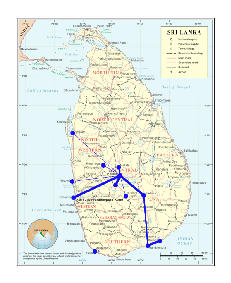
\includegraphics[height=0.3\textheight]{pics/Kandy-network}
 % Kandy-network.jpg: 478x600 pixel, 362dpi, 3.35x4.21 cm, bb=0 0 95 119
 \caption[Strength of contacts between Kandy and other towns]{Impressionistic strength of contacts between Kandy and other towns, and between Badulla and the South}
 \label{fig:Kandynetwork}
\end{figure}

Contact with Colombo was also very frequent (at least after independence), and most Malays from Kandy have relatives in Colombo. Other than that, one speaker from Kandy had her mother from Negombo, to the North of Colombo, and  another's mother is from Puttalam. The wide-spread kinship ties of the Malays prove that in the last three generations, the Malay network covered all of the Upcountry and the western coast with Colombo and Negombo. It is less common to have relatives in the South (Hambantota, Kirinda); this community seems to form a separate network \citep{AnsaldoEtAl2006fel,LimEtAl2007}. There are some Malays in Galle, who still speak Malay, but who seem to be quite isolated from the rest. Figure \ref{fig:Kandynetwork} gives an impressionistic illustration of the perceived strength of ties. Further, more sophisticated demographic research must show whether the postulated strengths of ties hold up to statistical analyses.


The Malays in Kandy have long been organized in cultural associations, the oldest one of which is the Kandy Malay association. Recent years have seen a number of schisms and splits among the Kandy Malays, leading to the foundation of the \em Hill Country Malay Club \em and the \em Hill Country Malay Association\em. The Malays in Kandy take part in island-wide cultural activities, such as singing, dancing, and sport events. In distinction to certain strata of Colombo society \citep{AnsaldoEtAl2006fel,LimEtAl2006aclcwp}, there seems to be little interest in teaching Malaysian Malay in Kandy, and attempts to speak Malaysian Malay are occasionally derided as \em Thuan thuan language\em, imitating the reduplicating pattern found in Malaysia, but not in Sri Lanka.

While in the surrounding Upcountry towns, the Malay language seems to be regularly transmitted to the younger generation, this seems to be less the case in Kandy, where English and Sinhala have made inroads into the domain of child care.

% \begin{table}
% 	\centering
% 		\begin{tabular}{lll}
% 		A & Sudhumpola	& 25	\\
% 		B &	Katuakalle 	& 20	\\
% 		C &	Mulgampola  &	20\\
% 		D &	Siyambalapitiya & 10	\\
% 		E & Heerassagala 	&	 30, scattered\\
% 		F &	Bowala, Dangole& 10	\\
% 		G &	Peradeniya &	2\\
% 		H &	Rosawattha& 30	\\
% 		I &	Nuwara Dodawala& 6	\\
% 		J &	Deiyannewella&	10\\
% 		K &	Bahivavakonda &	2\\
% 		L &	Asgiriya &	3\\
% 		M &	Malnaiyama&	10\\
% 		N &	Buwelikada & 10	\\
% 		O &	Wewelpitiya & 0	\\
% 		P &	Ampitiya &	5\\
% 		Q &	Lewella & 10	\\
% 		R &	Mapanawatura &	1\\
% 		S &	Mawilmada & 6	\\
% 		T	&	Kathugasthota & 20 \\
% 		U & Kahalla 5 &	\\
% 		V &	Watupuluwa &	0\\
% 		V &	Malwattha &	0\\
% 		V &	Kotugodella &	0\\
% 		V &	Kandy Town &	15\\
% 		V &	Hanthane &	3\\
% 		\end{tabular}
% 	\caption{List of Malay families in quarters of Kandy}
% 	\label{tab:ListOfMalayFamiliesInQuartersOfKandy}
% \end{table}
% 
% \begin{table}
% 	\centering
% 		\begin{tabular}{ll}
% 		 \textbf{Matale}	& 50	\\
% 		 \textbf{Kurunegala}	& 170	\\
% 		 Nawalapitiya	& 150	\\
% 		 Gampola	& 200	\\
% 		 Kegalle	& 30	\\
% 		 Nuwara Eliya	& 20	\\
% 		 \textbf{Badulla} 	& 175	\\
% 		 \textbf{Bandarawela}	& 50	\\
% 		 \textbf{Hatton}	& 25 \\
% 		 Ratnapura	& 20	\\
% 		 Balangoda	& 20 \\
% 		 Passara	& 15 \\
% 		 Badalkumbara	& 10	\\
% 		 \textbf{Hambantota}	& 200	\\
% 		 \textbf{Kirinda}	& 50	\\
% 		 Galle	& 60\\\citep[86,113]{Saldin2003}
% 		 Puttalam	& 100	\\
% 		 Chilaw	& 20	\\
% 		 Anuradhapura	& 25 \\
% 		 Mineeriya & 25	\\
% 		 Mihinthale	& 10 \\
% 		 Trincomalee	& 75	\\
% 		 Batticaloa & 10	\\
% 		 Matara	& 20	\\
% 		 Polonnaruwa & 20 \\
% 		 \textbf{Colombo} & 1000\\
% 		\end{tabular}
% 	\caption[List of Malay families in Sri Lankan Towns]{List of Malay families in other Sri Lankan Towns. Boldface indicate good preservation.}
% 	\label{tab:ListOfMalayFamiliesInOtherSriLankanTowns}
% \end{table}




% %"`During the Dambadeniya period (1220--1293 A.D.)Javanese Forces headed bx Chandrabhaanu who professed to be a Buddhist, had made an attempt to invade Sri Lanka.  Thi sattemot was successfully repulsed bz the Sinhalas. [...] The beginnings of Malay/Javanese linguistics influence on the Sinhala language could therefore be traced from about the beginning of the Polonnaruva period (1098--1234 A.D.)"'\citep[97]{Sannagala}


\section{Relation to the Moors}\label{sec:slmbg:RelationtotheMoors}

In all academic studies about SLM, with the exception of
\citet{Jayasuriya2002} and Ansaldo's work, a strong emphasis on the contact between
the Malays and the Moors\footnote{Some Moors resent the term `Moor' for their ethnic group and prefer `Conakar/S\=onahar'.
 `Moor' goes back to the Portuguese who designated Arabs as `Moros', while `Conakar' goes back to Tamils who designed first Greeks and then Arabs that way \citep[2]{Hussein2007}, so neither of those is a native term \citep[45]{Nuhman2007}. In the course of history, there has been a heated debated among this community whether one should identify as `Moor' or `Muslim' \citep[42ff]{Nuhman2007}. I follow academic usage in employing the term `Moor', which furthermore has the advantage of being less ambiguous than `Muslim'.}
is found. This has been called the `Tamil bias' \citep{Ansaldo2005ms,Ansaldo2008genesis}. The proponents of a close link between Malays and Moors argue that the two minorities shared Muslim faith and were thus natural allies in a predominantly Buddhist and Hindu country under Christian colonial reign. This is also used to explain the linguistic shape of SLM,
because  Moor women married to Malay men would have acquired an
imperfect Malay that they passed on to their children. This
imperfect acquisition would be at the base of modern SLM.
\citet{Ansaldo2005ms,Ansaldo2008genesis} criticizes that the historical evidence provided for this scenario is not up to scientific standards, and that oral history of the Sri Lankan Malays suggests that extensive intermarriage with the Moors did not happen.\footnote{Ian Smith (p.c.) remarks that Malays have a political interest in being seen as separate from the Moors (see Section \ref{sec:slmbg:postreg:Political history} above), and that, therefore, they might be downplaying their Moor heritage.}

On analyzing the references in the literature one finds that the claim of close contact to the Moors is mainly based on \citet{Hussainmiya1987, Hussainmiya1990}. The theory does not lack plausibility and is supported by some historical sources. But  Hussainmiya often argues on intuitive grounds and the sources for certain of his claims are not given or vague. He himself  (1987:45) says that ``the details of the nature of mutual contacts between these people cannot be documented.'' Let's take a close look at what he presents.

The argument is based on:

\begin{itemize}
    \item the gain in Islamic knowledge
    \item the Moors helped a Malay prisoner
    \item Christopher Schweitzer's report
    \item the Dutch \em tombos \em and Sri Lankan \em Kadutams \em
    \item a cultural comparison with Malays in South Africa
\end{itemize}

\citet[43]{Hussainmiya1990} argues that Malays in Ceylon must have had contact with great Islamic scholars. Thus, a certain exile named Radin Adipati Natakusuma was banned to Ceylon in 1743. When he returned to Jogyakarta in 1758, he was made chief of the religious officials there. A similar case is that of Wirakusuma, who became the leader of a religious group on returning. Other exiles are said to have become
pupils of the Islamic teachers Sayyid Musa Ngidrus and Ibrahim Asmara in Ceylon. This is seen as evidence for contact between the
exiles and Islamic scholars in Ceylon.  Whether these scholars were Moors is a different question. \citet{Wieringa1997} informs us that Ibrahim Asmara was an Islamic apostle from Champa (today's Vietnam), and as such it is unlikely that he was a Sri Lankan Moor.  It remains furthermore
questionable whether the normal soldiers would have undertaken thorough religious studies in Ceylon.

The second piece of evidence are minutes from the Dutch Political Council Colombo, suspecting the Moors of aiding exiled Malays in communicating with each other.

The third piece of evidence is a report of a German employee of the \textsc{VOC}, Christopher Schweitzer, from 1680, taken as evidence for Malay-Moor intermarriage by \citet{SmithEtAl2006cll}.

\begin{quote}
    Their language is Ambonese, but the majority also speak Malay, Sinhala, Portuguese and Dutch. \el{} The wives, who in part are Ambonese, in part Sinhalese and Malabarian may not say anything [against the stripping of their ornaments]. \citep[106]{Schweitzer1931} [my translation]\footnote{\el ihre Sprach ist Ambonesisch können aber meistentheils ach Malley- Singules- Portuges- und Holländisch \el die Weiber, welche theils Ambonesin, Singulesin und Malabarin, dörffen nichts darzusagen.}
\end{quote}
 


It is difficult to find evidence for contact between the Malays
and the Moors in this passage. There are of course the Malabarian
wives, with \em Malabarian \em being an old word for  ``person speaking a South Indian language'' (mostly Tamil) \citep[cf.][92]{Rogers1990}.
But nothing is said about their religion, so Hindu Tamils cannot be excluded \citep[cf.][68]{Hussainmiya1987}. There are also Sinhalese and Ambonese wives, and the soldiers are not even mentioned to speak Tamil,\footnote{Interestingly,
 \citet[45]{Hussainmiya1990} affirms that ``soldiers also spoke Sinhala and Tamil.'' How he finds this in Schweitzer's text is not clear to me.}
only Malay, Sinhala and the colonial tongues. If one has to rely on this fragment of text, then it surely does not support a close contact between Malay soldiers and the Moors, because this would have resulted in knowledge of Tamil rather than Sinhala.

The fourth piece of evidence are the Dutch \textit{tombos},  particularly the head tombo available at the Sri Lanka National Archive 1/3758, in which  a number of cases of intermarriage are said to be reported. Unfortunately, Hussainmiya does not give the numbers, so it is difficult to evaluate this claim. He (1987:25) also cites Lankan marriage registers (\textit{Kadutams}) that are in his possession and that also list intermarriages. These registers could not be consulted for this book.

\citet{Ansaldo2008genesis}  checked these claims against the photocopies of the Sri Lankan National Archive stored in the Dutch Nationaal Archief in the Hague. He reports that the tombos are inconclusive at best:
 

\begin{quote}
1. The records for the period up to 1796 are damaged by water, making significant
parts of the entries illegible. The most revealing information for identification
here are the signatures of the parties. There is however hardly any information of
ethnic group, which makes it difficult to identify Malay/Indonesian and Moors
given that both groups share the practice of adopting Arabic names. In a
particularly interesting section in the tombos dedicated to mixed marriages (cf.
Hussainmiya 1987), only five of 238 entries clearly refer to individuals of
Javanese origin: of these, two records refer to Javanese-Moor marriages, one to a
Javanese-Javanese marriage, and the remaining two are unclear.\\
2. The following period until 1919, albeit under British rule and therefore less
interesting for our claim, shows a more structured archiving system where
indication of race is given. Where legible, this reveals still a majority of Western
marriages, a growing number of marriages between Eurasians and Burghers
(locally born of Dutch/Western heritage), and between Burghers. There are two
clear entries involving Malays, one married to a Eurasian (between 1867-1897),
and one to a Burgher (1885-1897). From 1897 onwards, race is clearly specified;
of 196 entries only one is Malay. \citep{Ansaldo2008genesis}
\end{quote}

Given the little intelligence which could be gathered, \citet{Ansaldo2008genesis} conducted some pilot interviews with Colombo Malays, who professed not being aware of intensive Moor intermarriage in their ancestry. The time-depth, and breadth of these interviews is limited of course, but they can be complemented by native amateur genealogy. \citet{ArfinBurah} has compiled a book about his genealogy, tracing his origins back to the Javanese exiles. This book contains 303 instances of marriages where both partners are mentioned. One of the partners is in the lineage of the exiled princes and is therefore Malay. The group membership of the other spouse varies. While the ethnicities of the spouses are not mentioned, their names often clearly indicate their background. In Sri Lanka, names can indicate which group the bearer belongs to. European first names are indicative of Burghers or other Christians, e.g \em Coralie Nadine Caspersz \em (Burgher) or \em Wilson Gunaratna \em (Sinhalese Christian). Sinhalese last names (like \em Gunaratna\em) indicate that the bearer is either a Sinhalese Buddhist or a Sinhalese Christian. Tamil last names (like \em Arulambalam\em) can either point to Tamil Hindus or Tamil Christians. Many general purpose Muslim names exist which are borne by Moors and Malays alike \citep[cf.][]{Hussainmiya1987, Ansaldo2008genesis}, e.g. \em Fatima\em, but some names are borne exclusively by Malays.\footnote{\citet[436]{Hussein2007} contains a list of common Malay names. Also see \citet[8]{Hussainmiya1987}} Cases in point are the first names \em Tuan \em and \em Gnei \em or the last names \em Dole \em or \em Sourjah\em. I am not aware of any names which are exclusively borne by Moors. Finally, there are some names in the list which cannot be classified in this schema, very often because they are not complete (e.g. \em Mina\em). Table \ref{tab:slmbg:marriage} breaks down the spouses of the descendants of the exiles. A list of the marriages retrieved is found in the appendix (p. \pageref{sec:marriages}).\\

\begin{table}[h]
\begin{tabular}{rcccccc}
	& Malay & general Muslim & Sinhalese 	& Tamil & Burgher 	& Unclear\\
absolute& 189	& 73		& 14		& 3	& 9		& 15\\
relative& 62.4\%& 24.1\%	& 4.6\%		& 1.0\%	& 3.0\%		& 4.6\% \\
relative w/o unclear cases&65.6\% & 25.3\%&4.8\%&  1.0\%   	& 3.1\%		& / \\
\end{tabular}
\caption[Provenience of spouses of Malays]{Provenience of spouses of Malays in \citet{ArfinBurah}. Total number of marriages: 303}
\label{tab:slmbg:marriage}
\end{table}

The column `general Muslim' mentioned above must be partitioned between Malays and Moors. How this split should be done is unclear, but we can set an upper limit to intermarriage with Moors: No more than a quarter of all contracted marriages involved a Moor. This holds true under the assumption that all instances classified as `general Muslim' actually refer to Moors. At least 2/3 of all Malay marriages did not involve a partner of another ethnic group. The upper bound for in-group marriages is 91.3\%, adding up `Malay', `general Muslim', and `Unclear'. Intermarriage with the Buddhist and Christian community is present but not common; both in comparable proportion of about 4\%. Intermarriage with the Tamil Hindu community is quasi non-existent. Marriage with non-Muslims is found in about 9\% of the cases, but the names given to children of such unions indicate that those families followed Muslim (and indeed Malay) naming practices for their offspring.

The genealogy of the exiles treated in \citet{ArfinBurah} spans about 200 years. It  starts with the exiles in the 18$^{th}$ century and goes through various positions in the Regiment, ending in civil professions in the 20$^{th}$ century. It appears that the offspring of the exiles touches all important domains for Malay culture, and it is unlikely that the marriage pattern followed by the individuals surveyed here is completely unrepresentative of the community as a whole. It seems fair to assume that between 10-15\% of all marriages involved a Moor partner.\footnote{This percentage seems to be valid for the present day as well. \citet[39]{Bichsel} reports that among the   Malays she interviewed, there had been 12 cases of intermarriage with Moors, either by them (22 consultants) or by their parents (44, if none of the consultants where siblings). The ratio is thus 12/66=18.2\%. However, the pattern does not seem to be uniform: \citet[417]{Nuhman2007} reports that in 1956 and 1960 more Malays married outside their community than within. \citet{Ansaldo2008genesis}, on the other hand, reports that ``of approximately 50 families interviewed in total, only two revealed genealogies including Moor-Malay
intermarriage.'' More demographic research is thus needed.} While this reflects the privileged positions of the Moors as compared to the other groups, it is not obvious that this rate of intermarriage would have had a significant effect on the evolution of the language.

Based on \citet{ArfinBurah}, the extent of intercommunal marriage totals about 20\%. As far as the regiment Malays are concerned, the percentage might have been even lower. The British Major Skinner ``attributed the financial difficulties of Malays to continuous inter-marriage in the regiment, and the resultant growth of `swarming connection' of soldiers'' \citep[119]{Hussainmiya1990}. The use of `intermarriage' in this context is not about marrying \em outside \em the regiment, but rather \em inside \em the regiment, i.e. with other Malays.


The fifth piece of evidence is of a rather speculative nature and compares the fate of the Malays sent to South Africa with the Sri
Lanka Malays. The Malays in South Africa have completely lost their original language and culture, which is attributed to the
absence of a coreligionist community such as the Moors in Lanka, which would support them. From the fact that the Malay culture has
not been lost in Sri Lanka,  \citet[53]{Hussainmiya1990} concludes that this must be due to the Muslim community of the Moors. While such an analysis is possible, it has to be mentioned that the disappearance of the Malay element in South Africa has surely more causes than just the
presence or absence of another minority, and that even the presence of a strong Moor community in Ceylon has not prevented Malay culture from being lost in the 20$^{th}$ and 21$^{st}$ centuries. Such a monocausal explanation should be handled with care.

To sum up, we have  the  transfer of Islamic knowledge to some exiled princes; Dutch suspicions;  dubious attested intermarriages in the \em tombos\em; Schweitzer's report, which casts doubt on the relation between Malay soldiers and Moors; and a speculation about South African Malays, which is, well, a speculation. This is far from being solid evidence for a close Malay-Moor relationship or linguistic influence from Tamil. Future research should be aware of the shakiness of these assumptions and take a more sceptical approach, like \citet{Ansaldo2005ms}.

After discussing the points that are said to be evidence for a close relation between Malays and Moors, I would like to briefly shed light on some more facts which make pervasive intermarriage unlikely: At least in the Upcountry, many Malays still have   distinctively South East Asian features, and can easily be told apart from Sinhalese, Tamils, and Moors, which look more South Asian \citep[416]{Hussein2007}. If intermarriage had been that rampant, we would expect that the South East Asian features would have been submerged by now. While South East Asian physical features are easy to be found in the Upcountry, this does not mean that all Malays in the Upcountry look like Indonesians. The spectrum stretches from prototypically Indonesian to prototypically Lankan, with all combinations in between. My point is not that no intermarriage took place, only that it was less pervasive than assumed in the literature. This is reflected in conflicting testimonials from foreigners having come to Sri Lanka at different points in time. \citet[115]{Percival1803} remarks:

\begin{quote}
Although the Malays intermarry with the Moors and other castes particularly in Ceylon and by this means acquire a much darker colour than is natural to a Malay; still their characteristic features are so striking predominant, that they cannot be mistaken.
\end{quote}

Over a century later, a visitor from abroad noted

\begin{quote}
Meeting Ceylon Malays there one cannot help noticing that some of them have the features of Javanese while others look like Malays and their personal names incline to both Javanese and Malay.
  (Said 1926 \nocite{Said1926}, cited in Hussainmiya 1987:34)
\end{quote}

Again half a century later, the former Malaysian Prime Minister Tunku Abdul Rahman remarked in the Malaysian newspaper \em Star \em in June 1981:

\begin{quote}
 They look more like Indians \el{} than Malays and their language is strongly influenced by the Indian dialect. \el{} [A]fter generations of intermarriage, it is hard to pick one from the other Malays, or the Moors, except when they themselves announce their racial identity. \citep[7]{Hussainmiya1987}
\end{quote}

These quotes are of course impressionistic, but show that different people had different impressions about Sri Lankan Malay appearances. If anything can be drawn from those quotes, it is that the Malays became more Indian-like over the course of time. While in the early 19$^{th}$ century, their ``characteristic features are so striking predominant'', and in the early 20$^{th}$ century they ``have the features of Javanese'', in the late 20$^{th}$ century ``they look more like Indians''. These quotes do not support the view that heavy intermarriage was going on in the early days. However, it is most likely that these three different people each met only a tiny subset of Sri Lankan Malays, and that their reports are valid for that subset only. Hence, they do not reflect a global appreciation, and cannot be used as exact sources. As stated above, even today the Sri Lankan Malay community comprises everything from very Indian to very Indonesian, and depending on the Malay one meets, his ethnic identity is easy or impossible to ascertain. It is likely that Percival met Malays of a more Indonesian type, while Tunku met Malays of a more Indian type, but this should not lead us to hasty generalizations.


% Another piece of evidence which speaks against too close association with the Moors is the fact that in Kandy, the Moor community is much less present than in Colombo. While in Colombo, about a quarter of the population is Moor, in Kandy this is much less. Interestingly, the dialectal differences between Kandy and Colombo are slim. Now, there are two possible ways to explain this: either there were more Moors in Kandy in former times, or the linguistic change SLM underwent is not caused by the Moors.

At least in Kandy, the relations between the Malays and the Sinhalese are better than with the Moors. Many Malays do not speak Tamil anymore, while this is still the language preferred by most Moors.\footnote{Some Moors speak Sinhala (\citet[62]{Nuhman2007}, \citet[46]{Hussein2007}).} The Malays are traditionally loyal to the powers that be (\citet[52]{OsmanEtAl2008}, \citet[48]{Saldin2001}), first the colonial powers, then the Sinhalese \citep[cf.][35]{Bichsel}. Since the Moors were not associated with these powers, they are not held in very high regard. This former association with the colonial powers has also led the Malays to adopt a more `Western' lifestyle \citep[cf.][41]{Saldin2001}. All senior Malays asked about their youth affirmed that they used to hang out with Burghers, leading a `happy-go-lucky'-lifestyle \citep[27]{Hussainmiya1990}, which is unusual with Moors.\footnote{A penchant for gambling is already noted in early reports, e.g. \citet[106]{Schweitzer1931} or \citet[131]{Pieris1918}. The literary activities of the Malays may add a more intellectual overtone to this lifestyle, but this would not make them resemble the Moors more. To the contrary, Moors were known as a ``backward community''  \citep[95]{Hussainmiya1987}, unlikely to engage in literary pastime. Furthermore, Malays had the highest literacy among all ethnic groups in Sri Lanka, while Moors had the lowest \citep[48]{Marga1988}, cited in \citet[17]{Bichsel}. As for the present day conflation of Malays and Moors in government statistics, \citet[36]{Bichsel} remarks: ``[A] comparison of the statistics given for the Moors with that for the Malays in the tables in this paper shows clearly how greatly the communities differ.''} Today, most Malays have a very liberal interpretation of Islam, while the Moors tend to be more conservative. This difference in lifestyle again makes overwhelming intermarriage unlikely. \citet[35]{Saldin2003} reports that as far as education is concerned, Malays seem to be closer to Sinhala practices.

After screening the evidence, let us now turn to the plausibility of early contact with the Moors.
If we imagine the situation in the early days of the Malays in Ceylon, would contact between Malays and Moors be plausible?  Would exiles be interested in meeting Islamic scholars? This cannot be excluded, but it does not seem likely that theology was one of their major preoccupations. Islamic scholarship was even less of an argument for the soldiers, convicts and slaves, whose interest in advanced theological discussion can be estimated to have been rather low. The latter groups had, on the other hand, interest in finding a Muslim wife, if they had not brought their family \citep[47]{Hussainmiya1990}. However, intermarriage to non-Muslims is already present in the early days, as shown in \citet{ArfinBurah}.

A further problem for contact between Malays and Moors could be that the colonial powers of the Portuguese and the Dutch tried to contain Muslim influence. In 1626, the Portuguese expelled the Moors \citep[84ff]{DeSilva1972},\footnote{Also see \citet[72f]{Vlekke1943} for the motivations of the Portuguese.} who would settle around Batticaloa, then under Kandyan rule \citep[113]{Codrington1926}.
The Dutch  restricted their share of coastal trade, and forced many  Moors into agricultural life in the East of Ceylon \citep[42]{Hussainmiya1990}.

The Malays, on the other hand, were always close to the centers of colonial administration \citep{Ansaldo2009book},  either because they had to be guarded, in the case of the exiles, or because they were the guards of the colonial power in the case of the soldiers.

After the middle of the 18$^{th}$ century, the percentage of free Malays grew \citep[49]{Hussainmiya1990}, and free Malay could easily enter in contact with the Moors. But the Malays liked to stay close to  their community,\footnote{\citet{Ansaldo2009book}  even argues that \em endo\em gamy was a defining feature of the SLM community at that point in time, rather that \em exo\em gamy as claimed by \citet{SmithEtAl2004} and \citet{SmithEtAl2006cll}.} and the Dutch had just pushed the Moors away from the colonial cities (Batticaloa is an exception to this, and maybe Trincomalee).\footnote{It is interesting that the British later would refrain from stationing a Malay Regiment in Batticaloa.}

Starting in 1783 the Malays had their own mosques, which continued to provide services in Malay afterwards.

\begin{quote}
    As the Malay community grew in numbers, and with the patronage extended by the colonial rulers, their religious needs were fulfilled according to Malay traditions. As the Malays claimed, special mosques for their congregations were set up in the Malay-majority townships, while they were ministered by special Malay \textit{Khatibs} or priests (as styled by the Malays). The Malays also had their own religious \textit{Kitabs} and legal texts written in [t]he Malay language.  \citep[19]{Hussainmiya1987}
\end{quote}


Religion was clearly a domain where the Malays affirmed their identity. Of course, the Moors were fellow Muslims, but it seems that the mosque was not so much a place of interethnic contact but a place of affirmation of group identity \citep{Hussainmiya1987}. Influence through religion could have taken place before 1783 or after 1930, when Tamil began to replace Malay as the language of the mosque \citep[23]{Bichsel}.

%\begin{quote}
%   ``the details of the nature of mutual contacts between [the Malays and the Moors] cannot be documented''\citep[44]{Hussainmiya1987}
%\end{quote}
%
%
%Hussainmiya says that Malays cannot be identified according to their culture, so basically, a Malay is a person that identifies herself as Malay.

%\begin{quote}
%   ``Schwitser did not mention about the religious background of the Amboinese, and it may be that they were not followers of Islam, which explains partly why only Sinhalese and Malabar (Tamil) wives are mentioned in this case. Or it may be that the `Moorish' women were included in the racial terms of `Malabaris'.''\citep[68, footnote 68]{Hussainmiya1987}
%\end{quote}
 



% \begin{quote}
%     ``Intermarriage with other races took place among the Malays [during the time of the Unique Malay Club] \el [at one stage in the nineties the key office bearers of the Uniques were children of non-Malays or, were married to non-Malays]''\citet[83f]{Saldin2003}
% \end{quote}

% \begin{quote}
%     ``In Malaysia and Indonesia it is the groom who gives the dowry, unlike in Sri Lanka, where the bride provides the dowry.''\citet[2]{Saldin2003}
% \end{quote}
% 
% 
% \begin{quotation}
%     ``There are no restrictions on interethnic marriages in Sri Lanka, and there has been intermarriage between the Sinhalese and the Sri Lankan Malays''\citet[9]{Jayasuriya2002}
% \end{quotation}


\section{Language issues}\label{sec:slmbg:LanguageIssues}
After looking at the sociohistorical development of the SLM community, it is now possible to investigate some questions of a more linguistic nature. The first such question is the origin of SLM. Other questions concern the development of the language in Ceylon, neighbouring languages, and the relative importance of different contact languages over time.

\subsection{Sources in the SEAA}\label{sec:slmbg:SourcesintheSEAA}
What are the linguistic ancestors of Sri Lanka Malay? It is clear that the Sri Lankan Malays ultimately came from South East Asia, but which languages or dialects from which islands contributed to its genesis? People from many different islands arrived in Sri Lanka as soldiers after having spent a variable period in Batavia/Jakarta before  sailing off to a battlefield. During the stay in and around Batavia, this soldier population began to acquire a distinct identity, distinct from the Javanese and Sundanese  of Java \citep[174]{Vlekke1943}.\footnote{\citet[99]{Raben2000} actually supports the idea that group identity in Indonesian societies of the time  was generally \em not \em created through ethnicity, but rather through ``personal attachments and charismatic power.''} \citet[14]{SmithRH} argues that  no single mother tongue could impose itself, and the lingua franca of the SEAA, a variety of Malay, was chosen for interethnic communication. % \citep[also cf.][174]{Vlekke1943}.

This variety has been given various names, among which Vehicular Malay \citep{SmithRH}, Trade Malay \citep{Ansaldo2005ms} and Bazaar Malay need to be mentioned.\footnote{It should be noted that Bazaar Malay can also refer to other varieties \citep{Paauw2003}.} Like most trade languages, Vehicular/Trade Malay was not monolithic and would be adapted to the communicative needs of speakers of different ethnic groups in different ports, with different influences from native languages. The sociolinguistic situation of Batavia/Jakarta is traditionally very complex. \citet[132]{Vlekke1943} states that ``in seventeenth century Batavian \el [i]n some respects, the confusion of languages was like that of Babylon''.
 \citet{AdelaarEtAl1996} list the following relevant varieties for the Jakarta region: \em Java Malay, Java Port Malay, Jakarta Malay (Betawi), Jakartan Indonesian, \em and \em  Tangsi Malay\em. It is beyond the scope of this study to investigate the sociohistorical developments of these varieties, but see \citet{Grijns1991} or \citet{Paauw2004,Paauw2008phd} for some discussion.

This complexity suggests that there were many input languages which participated in the formation of SLM. The
different homelands of the Malays arriving have contributed to a
greater or lesser extent to SLM as we know it today. \citet{Bakker1996stuf,Bakker2006} claims that  ``it is fairly well known what Malay looked like  when it was imported to the island by the Dutch''. This opinion is maybe a bit optimistic given that the exact nature of the language (or languages) that the new immigrants spoke is far from clear to the remaining researchers. The total absence of written records from that period does not make the task any easier.
 What can be done is to look at
several features of present day SLM and trace them back to Malay
varieties of the SEAA. This endeavour has been undertaken by
\citet{Adelaar1991}.
He finds that Moluccan, Bazaar Malay, Baba
Malay and Jakartanese have contributed most to SLM, besides the notwithstanding influence of Tamil and Sinhala (Table \ref{tab:slmbg:Adelaar1991}). \citet{Paauw2004} critically reassesses the data and analysis by Adelaar and comes to somewhat different results. He finds that many of the features of SLM are found in several varieties of Vehicular Malay (VM), so that they cannot be attributed to any single variety. Furthermore, he traces more of the features to adstrate influence from Tamil, and discards most of the Moluccan influence, as well as all of Baba and Bazaar influence.


\begin{table}
\begin{tabular}{rp{4cm}p{4cm}p{4cm}p{2cm}}
	& Standard Malay & Sri Lanka Malay & Adelaar &  Paauw\\
\hline
1) &  *h> 		& h*h> Ø & Moluccan, Bazaar, Baba, Jakartanese &  general VM \\
2) &  		& retroflex series & (Tamil and Sinhalese )&  Tamil \\
3) &  		& (contrastive) vowel length & (Tamil and Sinhalese )&  Tamil \\
4) &  		& (contrastive) consonant gemination & (Tamil and Sinhalese )&  Tamil \\
5) &  m/n/\ng/ 	& \ng	&Moluccan&  *Tamil \\
6) &  \E	& i/u or \E{} varying with i/u 	& Moluccan &  *Tamil \\
7) &  retention of most of the inherited morphology
		& loss of most of the inherited morphology & Moluccan, Bazaar, Baba [...] &  general VM \\
8) &  locative preposition +noun phrase
		& noun phrase + linker + locative preposition & Bazaar&   Tamil \\
9) &  noun + determiner
		& determiner + noun &  Moluccan, Bazaar, Baba, Jakartanese&  general VM \\
10) &  possessed + possessor
		& possessor + linker + possessed &  Moluccan, Bazaar, Baba, elsewhere&  general VM \\
11) &  noun + adjective
		& adjective + noun &  (Tamil and Sinhalese)&  Tamil \\
12) &  prepositions
		& postpositions & (Tamil and Sinhalese)&  Tamil \\
13) &  subject-verb-object
		& subject-object-verb & (Tamil and Sinhalese)&  Tamil \\
14) &  ada denoting existence of a noun
		& ada/\E r\E: progressive aspect of a verb & Moluccan, Bazaar, Baba&  *Tamil \\
15) &  		& negators: t\E r/tra &Moluccan, Baba& Moluccan\\ 
16) &  full tense-mood-aspect adverbials &  full and reduced tense-mood-aspect adverbials & Moluccan, Baba&  general VM \\
17) &  plural personal pronouns are independent lexemes
		& plural personal pronouns are historically compound forms with *ora\ng{} & Moluccan, Bazaar, Baba&  general VM \\
18) &  		& 1$^{st}$ and 2$^{nd}$ personal pronouns borrowed from Hokkien Chinese & Bazaar, Baba, Jakartanese&  Jakarta Malay \\
19) &  		& plural marker pada 	& Jakartanese& Jakarta Malay \\
\end{tabular}
\caption[Origin of SLM features according to \citet{Adelaar1991} and \citet{Paauw2004}]{Features distinguishing Sri Lanka Malay from Standard Malay, and their origins according to \citet{Adelaar1991} and \citet{Paauw2004}. Features which Paauw argues to be misanalyzed by Adelaar are marked with an asterisk *.}
\label{tab:slmbg:Adelaar1991}
\end{table}
 
\citet{Paauw2004} further undertook an etymological analysis of the lexicon.
His findings are presented in table
\ref{tab:originsOfTheSLMLexicon}. In this table, origin \textit{Sri Lanka} means all words that joined the vocabulary after the language had reached Ceylon, and includes Tamil, Sinhalese, Portuguese, Dutch and English words. \textit{Common Malay} indicates words understood in every part of the Malay world, whereas \textit{Indonesian} words mostly come from Betawi or Javanese and are not understood outside Indonesia. \textit{Malaysia}, finally, indicates words from the peninsula.

\begin{table}
    \centering
        \begin{tabular}{l|l}
                        origin      & percentage\\
                        \hline
                        Sri Lanka &       10,0\% \\
                        Common Malay &    55,7\% \\
                        Indonesia &       11,7\% \\
                        Malaysia &        0,6\% \\
                        Loan Words &      21,7 \% \\
        \end{tabular}
    \caption{Origins of the SLM lexicon according to \citet{Paauw2004}}
    \label{tab:originsOfTheSLMLexicon}
\end{table}

\citet{Paauw2004} concludes that ``the Malay variety most likely responsible for the lexification of Sri Lanka Malay was a variety originating in Jakarta, and that Moluccan Malay and the Malay of the Malay peninsula also contributed, in a more limited manner.''
Two features which Adelaar and Paauw have not addressed actually corroborate this analysis: SLM has words with schwa in the final syllable (e.g. \phontrs{\dentt a:n@m}{plant}), typical of Jakarta \citep{Adelaar1985}, and SLM drops schwa in antepenultimate position (\phontrs{cri:\dentt a}{story} compare Std. Malay \em c\E rita\em). This is also common in Jakarta (Uri Tadmor, p.c.). Phonological influence from Malaysia is noted by \citet{Paauw2004} in the lowering of high vowels in the last syllable as compared to Indonesian, e.g. \phontrs{ma:sok}{enter}, compare Indonesian \em masuk\em, although \citet[99]{Paauw2008phd} states that in Eastern contact varieties of Malay this lowering can also be found.

% While lexical influence from Malaysia is surely limited, the vowel lowering is very regular and pervasive. The possibility that the language had already stabilized when the first immigrants from Malaysia arrived (1819) gains some support from the lack of lexical influence, but is weakened by the phonological impact these immigrants had. Further research will be needed to ascertain the relative importance of Malaysian vocabulary against phonology.
 

\subsection{Three theories of genesis}\label{sec:slmbg:Threetheoriesofgenesis}
It is a fact that Sri Lanka Malay as spoken today is strikingly different from any other Malay variety. It must have undergone radical language change in the last 350 years \citep{AnsaldoEtAl2009age}. There are competing theories as to how this language change came about, and by what it was triggered. The idea defended by Hussainmiya, Smith and Paauw in their publications \citep{SmithRH, SmithEtAl2004, SmithEtAl2006cll} is that SLM is the product of intermarriage between Malay men and Moor wives, who spoke Tamil. The Tamil speakers would then try to acquire the language of their soldier husbands,   very much like the slave populations in the Caribbean tried to acquire a European language. The language learners would transfer grammatical structures of their original language into the target language. This means that a strong Tamil substrate would remain in the  variety spoken by the wives, which would then be passed on to the children, and by and by generalize to the speech of the whole community. This scenario of genesis is then very similar to the genesis scenario proposed for  Sri Lanka Creole Portuguese \citep{Smith1979}, where the indigenous Tamil population of Batticaloa tried to acquire Portuguese and imposed Tamil grammatical structures on that language. This theory of genesis fits well with the Relexification Theory \citep{Muysken1981,Lefebvre2001} of Creole genesis, where we find a combination of the grammar of the substrate with the lexicon of the superstrate.  In Lefebvre's account of Haitian Creole, the West-African language Gbe would be the substrate and French the superstrate; for SLM, Tamil would be the substrate and the language of the immigrants the superstrate.

A somewhat different position is taken by \citet{Bakker2000convergence,Bakker2000rapid,Bakker2006}, who argues that the variety spoken in Sri Lanka was not heavily influenced by the local languages until the end of the 19$^{th}$ century, citing  documents written by military officers which comply with the general Malaysian/Indonesian standard. Only after the disbandment of the regiment in 1873 would there be heavy language change toward   Tamil (and possibly Sinhala), which would take place within one generation.

\citet{Ansaldo2005ms,Ansaldo2008genesis,Ansaldo2009book} finally proposes that the ecology of Sri Lanka Malay has more in common with settings of metatypy as described by \citet{Ross1996,Ross1997,Ross2007}. SLM would not be the result of intermarriage and  relexification, as proposed by Smith et al. Rather, SLM would be the product of the immigrants' having to handle three languages at the same time: Malay, Sinhala, and Tamil. Given that the grammatical markup of Sinhala and Tamil is very similar, and to lessen the cognitive burden of handling too many different constructions, SLM speakers would gradually emulate the Lankan structures they use everyday in Sinhala and Tamil in their own language as well. SLM would be the in-group language (\em esoteric \em in Ross's terms), which is influenced by the language(s) of wider communication (\em exoteric\em), in this case Sinhala and Tamil. This is analogous to the grammatical change of Takia (\em esoteric\em) towards Waskia (\em exoteric\em) in the Madang province in Papua New Guinea, as described by \citet{Ross1996}.

All these three theories of genesis are tied in one way or another to the historical facts, but they make different assumptions about the historical sociolinguistic setting. Some of these assumptions are explicit and some are implicit, some are supported by evidence, while others are not. In the following sections, I will discuss the socio-historical setting which is assumed for each of the three theories. This will be followed by an explanation of the mechanism which would have led to the change of the language.  I will then discuss the internal plausibility of the setting and mechanism assumed, before I turn to the  historical evidence  presented by the supporters of the particular theory.  This evidence is sociological on the one hand, and linguistic on the other. In the expository parts, I will not engage in criticism of the proposed theories. In the sections after the exposition, both linguistic and sociological evidence presented will be  discussed, critically evaluated, and weighed against other pieces of evidence not necessarily discussed by the supporters. Finally, every theory will be checked for its place in current theorizing on language contact. Does it comply with generally contact linguistic theory, or does it go against some basic assumptions and principles in the field?

For expository reasons, I will start with Bakker,  then turn to the Tamil substrate hypothesis as advanced by Hussainmiya, Smith and Paauw, and discuss metatypy as proposed by Ansaldo in the end.

\subsubsection{The rapid conversion hypothesis}
This argument was the first to be published \citep{Bakker1995nl}. It involves two components: SLM has converged towards Tamil (and possibly Sinhala), and this change happened rapidly. At first, this hypothesis argued that change took place between 1870 and 1906, but later versions \citep{Bakker2006} are more lenient as to the precise start and end dates of the rapid change. In the earlier versions of this hypothesis, convergence was the mechanism at work, while in later work, metatypy is also mentioned as a possibility. In this section, I will limit myself to the discussion of convergence. Metatypy will be discussed more extensively in Section \ref{sec:slmbg:metatypy}.

\paragraph{Argument}
Bakker first mentions Sri Lanka Malay in \citet[17f]{Bakker1995nl}, but the discussion is too brief to really distill any claims about its genesis (besides the analogy to Sri Lankan Portuguese). In \citet{Bakker2000convergence,Bakker2000rapid}, he develops that

\begin{quote}
[Sri Lanka Portuguese and Sri Lanka Malay] were documented in the early part of the last [=19$^{th}$ SN] century and in both cases it is clear that the languages were creolized at that point in time: they lost all person inflection, almost all derivation, and all morphological irregularities. Instead, these languages appeared to have preverbal markers for tense, mood and aspect, a system which may be considered typical for creole languages (Holm 1988)\nocite{Holm1988}. Word order is rather rigid SVO and the languages are typologically close to isolating. In short, they look like a prototypical creole. This, however, is only true for older stages of these languages.
\end{quote}

He then goes on to argue that modern SLP and modern SLM have become more complex and have departed from that creole typology. Bakker argues that ``the whole process took place in one or two generations.''\footnote{also in \citet[153]{Bakker2006}.} 
In \citet[607]{Bakker2000rapid}, he concludes

\begin{quote}
In the case of SLM we must \el{} assume a few decades at most for the radical changes, as earlier documents show a more ordinary form of Malay.

Thus, `convergence intertwining' may change a language structurally and typologically in just a few decades from isolating to agglutinative.
\end{quote}

\citet[152]{Bakker2006} gives some more indications as to the sources of his claims about earlier stages of the language: ``early sources (from 1806 or 1820 to the 1930s) show a form of Malay with little grammatical influence from Tamil.'' Furthermore, he claims that \citet{Hussainmiya1987} contains some instances of Tamilized features in early texts, which he discounts as minor.

Bakker's conclusion is somewhat puzzling:

\begin{quote}
The two main opinions on the matter of \em when \em the convergence happened both have to accept that it is a very rapid process. If it happened soon after arrival, \el{} the convergence or metatypy must have happened within one or a few generations. Alternatively, if it happened in the first half of the twentieth century \el{}, it must also have happened within one or two generations.
\end{quote}

The third possibility, that the change happened between arrival and the second half of the 20$^{th}$ century, as a continuous process, is not addressed.

\paragraph{Sociolinguistic setting assumed}
Bakker's hypothesis  makes few sociolinguistic assumptions. The main and most important assumption is that Tamil was present as an important adstrate during the whole period, while Sinhala influence is also possible \citep[46]{Bakker1995nl}.

\paragraph{Mechanism}
Bakker assumes convergence, or metatypy as defined in \citet{Foley1986} and \citet{Ross1996, Ross2001}.

\paragraph{Plausibility} If the premisses are as Bakker suggests, the developmental scenario he sketches is plausible, although not everyone will agree that language change can happen that quickly.  \citet{Ansaldo2005ms,Ansaldo2008genesis} and \citet{AnsaldoEtAl2007dcctr}, for instance, argue that rapid change is not a possibility for the restructuring of the case system we find in SLM. They argue that a restructuring of a whole functional system (like case) cannot be accommodated under the rapid conversion hypothesis and must necessarily be gradual, requiring more time than allowed for by Bakker.

\paragraph{Historical evidence}
Bakker refers to Hussainmiya's work for the historical evidence he needs, but does not indicate what parts, chapters or pages contain that evidence. It is likely that he refers to the \em Syair Kisahnya Khabar Orang Wolenter Benggali \em \citep[86]{Hussainmiya1987}, from 1820.\footnote{The nature of the earlier documents cited by Bakker, I have not been able to ascertain. Bakker (p.c.) affirms that he based his work exclusively on Hussainmiya. \citet[86ff]{Hussainmiya1987} contains a list of all early texts. None of them predates 1820.} The Syair should show that the Malays used a creole-like language in the beginning of the 19$^{th}$ century. As pointed out by \citet[178]{SmithEtAl2006cll}, this text is in Literary Malay, which, while sharing some features with Creoles (no person inflection, SVO word order), is generally not considered a creole. The linguistic composition of this text can be explained by the British having brought Malay teachers from the Peninsula, who taught Literary Malay to the officers, and is surely not a result of creolization in Ceylon.   \citet{SmithEtAl2006cll} argue that during the period of the Regiment, diglossia existed, with Literary Malay as the high variety and Sri Lanka Malay as the low variety, mirroring the general sociolinguistic pattern found in South Asia in general, and in Sinhala and Tamil in particular.\footnote{Whether
 the restricted use of Literary Malays by some officers can be called `diglossia' is open to debate, but it is certain that Literary Malay was not a language of widespread use in 19$^{th}$ century Ceylon.}
This is further corroborated by the fact that newspapers edited in Ceylon had subscribers in the SEAA \citep[89]{Hussainmiya1987}, who apparently could understand the language of the publication \citep[24]{Saldin2001}.

Bakker argues that the language emerged rapidly. He gives two possibilities for the rapid emergence: either shortly after arrival, or in the 20$^{th}$ century. For the `early' hypothesis, he does not present any historical evidence. He argues that if  diglossia involving `traditional' and `Tamilized' varieties existed in the 19$^{th}$ century, then the Tamilized variety must have developed very quickly, within one or two generations. It is not entirely clear to me why this would be necessary. For diglossia to be present in 1850, any time between 1650 and 1840 would be possible as a `start date' for the Tamilized variety, and more than two generations could be encompassed. As for the `late' hypothesis, he argues that until the middle of the 19$^{th}$ century, the Malays' language was very similar to other Malay varieties. He bases this claim on the existence of texts from that period which do not show Lankan features. Other texts he refers to are from the beginning of the 20$^{th}$ century, and show Lankan features. Thus, the language change must  have happened between these two points in time. Note that for the `early' hypothesis, Bakker assumes diglossia at 1850, while for the `late' hypothesis, he does not. Depending on the hypothesis to defend, his interpretation of the sociohistorical setting in the 1850s is different.

Bakker seems to have an `all-or-nothing' approach to diglossia in the 19$^{th}$ century. One variety must be High Malay, the other one must be either SLM as we know it today, or `Proto-SLM'. However, the possibility of gradual development of SLM cannot be ruled out. It is possible that `Early Low SLM', spoken during Dutch times, gradually evolved into `Modern Low SLM', spoken today, through the intermediate stage of `Middle Low SLM', spoken during British times. This variety would then be in a diglossic situation with High Malay, used in the British Regiment schools and the literary works. In order to argue for rapid conversion, one has to show that either `Early Low SLM'=`Middle Low SLM' with rapid conversion to `Late Low SLM'. Or one has to show that `Middle Low SLM'=`Late Low SLM', with rapid conversion taking place before, ideally within one or two generations. No proof for either of these equations has been brought forward.

\paragraph{Linguistic evidence}
Bakker shows that SLM shares many structures with Tamil, and also mentions similarities with Sinhala in passing. These structures back up his claim of convergence. Bakker does not use linguistic evidence to prove his claim of rapid development.

\paragraph{Counter-evidence}
Since there is no real evidence for Bakker's theory, counter-evidence to refute his claims is not necessary, strictly speaking. Counter-evidence against Bakker's claims can be divided into three domains: 1) against convergence, 2) against early rapid change, and  3) against late rapid change. As for 1), the claim that SLM grammatical structure is close to Tamil structure\footnote{And Sinhala structure for that matter.} seems pretty much uncontroversial, although some non-Tamil features remain in SLM \citep{Slomanson2006cll}. As for 2), since there are no documents available, it is very difficult to make any claims about the structure of SLM preceding 1800. 3), finally, is the only domain where true counter-evidence can be found. \citet{SmithEtAl2006cll} point out that the documents from the middle of the 19$^{th}$ century Bakker refers to are written in Literary Malay by officers who had had schooling in that variety. They argue that at that point in time, there was a diglossic situation, with SLM as the low variety and Literary Malay as the high variety. All literary production from that period is in Literary Malay and cannot be used to make any claims about the structure of the colloquial language. Another argument against the `late rapid change' hypothesis is the absence of strong dialectal differences in SLM.
If the claim is that SLM changed after the disbandment of the regiment which entailed catastrophic changes, we would expect that these changes would only affect the speakers who witnessed them. Speakers in remote places like Hambantota (settled in 1802), with little contact to the other communities, should not change their language \citep[cf.][]{SmithRH}. We would thus expect a linguistic difference between the `catastrophic communities' and the others. While there is some dialectal difference between Hambantota and the other dialects, it is mostly phonological. In any case, it does not point towards the Colombo community having had a significantly different development from the Kirinda community. If we find the same linguistic structures in Colombo and Hambantota, it makes no sense to attribute the structure of the Colombo dialect to some social changes which could never have affected  Hambantota.
 
\paragraph{Place in contact language theory}
The mechanisms of convergence and metatypy are well-established in contact linguistics, although the speed of development Bakker assumes is not a common feature of theories of language contact, and indeed metatypy is generally argued to be a gradual process \citep[127]{Ross2007}.

\subsubsection{The Tamil substrate hypothesis}
This hypothesis is implicitly present in \citet{Hussainmiya1990} and worked out in detail by \citet{SmithEtAl2004, Paauw2004} and  \citet{SmithEtAl2006cll}. It assumes that the development of SLM was analogous to the development of Sri Lanka Portuguese, and analogous to the development of Creole languages in other parts of the world. Speakers of a substrate language (Tamil in this case) try to acquire a superstrate language (Malay), but transpose the grammatical structures of their native language onto the language to be acquired.
 

\paragraph{Argument}
The Tamil substrate hypothesis states that ``SLM developed as a result of intermarriage between Malay men and Moor women,   vehicular Malay  thus served as its lexifier and Sri Lanka Muslim Tamil (SLMT) as its principal  substrate language'' \citep{SmithEtAl2004}.
This is explicated in more detail in the following two passages.

\begin{quote}
From their arrival, [the Malays] associated closely with the established Tamil-speaking Sri Lanka `Moor' community, with whom they  shared the Muslim religion \el. As the soldiers were single males for the most part, a high degree of intermarriage with the Moor community was inevitable. Through this interaction between the two communities, a new language arose with Tamilized structure and with a Malay lexicon. \citep[160]{SmithEtAl2006cll}
\end{quote}


\begin{quote}
From the earliest days in Sri Lanka, `Malays' has a close relationship with the Tamil-speaking `Moors' \el. Intermarriage was first noted by a German observer, Christopher Schweitzer \el, who also commented on the multilingualism of the Malay soldiers \citep[49--50]{Hussainmiya1987}, and was confirmed by Dutch \em thombos \em (administrative records) of the eighteenth century  \citep[52]{Hussainmiya1987}. An indigenized variety of Malay must have arisen among the children of these marriages, whose fathers spoke VM but may have even been familiar with Tamil through their interactions with the Moor community, and whose mothers spoke Tamil natively and must have attempted to learn Malays without the benefit of instruction. Tamil-speaking mothers must also have tried to make Malay the language of the home; otherwise it would be difficult to imagine the language being maintained by subsequent generations.
 \citep[176f]{SmithEtAl2006cll}
\end{quote}


\paragraph{Sociolinguistic setting assumed}
For this hypothesis, three sociological assumptions are fundamental: a) there was heavy intermarriage between Malays and Moors; b) Tamil was the substrate and Malay the superstrate, i.e. Malay had more prestige than Tamil; and  c) the children of bilingual parents acquired the non-native variety of the mother, rather than the native variety of the father. Furthermore, Smith and colleagues discard Sinhala as an important factor. Why this is done is not entirely clear. Presumably it is  because the recombination of the two components grammar and lexicon, which is the basis of the relexification model, is difficult to implement if the number of involved languages is not two.

\paragraph{Mechanism}
Although they do not state so explicitly, Smith and colleagues seem to adhere to a substratist school of creole studies. The idea is that grammatical structure from a substrate is carried over into the superstrate when the latter is learned. The new language is thus a recombination of substrate grammar and superstrate lexicon. Formalizations of this approach can be found for instance in \citet{Muysken1981} or \citet{Lefebvre2001}.

\paragraph{Plausibility}
The substratist/relexification theory is well-tested in many contact settings, and the argument as such is plausible if the assumptions are correct. However, the statement ``Tamil-speaking mothers must also have tried to make Malay the language of the home; otherwise it would be difficult to imagine the language being maintained by subsequent generations'' \citep[177]{SmithEtAl2006cll} is not completely plausible, as \citet{Ansaldo2008genesis} notes. He says that ``there [would] have been [no]  plausible reason for
Tamils/Sinhalese to restructure their own varieties in acquiring SLM; they were,
after all, speakers of larger, socially more prestigious languages in which the SLM
speakers would have been quite competent.'' To return to the original idea by \citet{SmithEtAl2006cll}: Why should Tamil mothers try to make Malay the language of the home? What incentive could they have had? They were speakers of a majority language after all. If, as Smith et al. argue, the Tamil mothers' keeping to Tamil would have posed a problem for the explanation of the maintenance of the language, there is an easier solution than assuming that they chose Malay as a home language: the amount of Tamil mothers was much more limited than what Smith et al. assume. As such, they could not exert as  important an influence. We will see in the following sections that the historical evidence suggests, indeed, that the extent of intermarriage has been overstated in the literature  (Also see Section \ref{sec:slmbg:RelationtotheMoors}).

\paragraph{Sociological evidence}
The historical evidence for intermarriage is said to come from Schweitzer's report and from the Dutch tombos. No evidence is presented as to the minority immigrant language being the superstrate and the local majority language the substrate. No argument is made why children would acquire the mother's non-native variety.

\paragraph{Linguistic evidence}
\citet{SmithRH} notes that Sinhala and Tamil are very similar in their markup, and notes left-branching word order, quotatives, case markers, and similar nominal and verbal categories. Smith notes that Hussainmiya claimed Tamil influence for SLM structures which could also have been of Sinhala influence, and that Jayasuriya claimed Sinhala influence for structures which could as well have been of Tamil influence. As a consequence, he investigates areas where Sinhala and Tamil differ, and finds that SLM is closer to Tamil in the areas he investigated, namely definiteness, number, animacy, and the accusative case. These findings are also used in later publications  \citep{SmithEtAl2004, SmithEtAl2006cll}. This would support a more intensive contact with Tamil speakers.

\citet{SmithEtAl2004} argue that, in the domain of phonology, SLM has a constraint which bans retroflex stops in initial position, just like Tamil, but unlike Sinhala.

\paragraph{Counter-evidence}
The hypothesis hinges on the assumption of heavy intermarriage with the Moor community. As argued above in Section \ref{sec:slmbg:RelationtotheMoors}, the evidence for intermarriage has been grossly overstated. This is not to say that there was no intermarriage. I just fundamentally call into question all the evidence which has been presented for \em heavy \em  intermarriage, which generally does not adhere to the standards of the field. For instance, in \citet[176]{SmithEtAl2006cll} we find again ``intermarriage was first noted by a German observer, Christoph Schwei[t]zer.'' It is true that Schweitzer talked about intermarriage in this passage, but this merits a full quotation to illustrate the quality of sourcing used to defend the Moor intermarriage hypothesis:

\begin{quote}
    Their language is Ambonese, but the majority also speak Malay, Sinhala, Portuguese and Dutch. \el{} The wives, who in part are Ambonese, in part Sinhalese and Malabarian may not say anything [against the stripping of their ornaments]. \citep[106]{Schweitzer1931}, [my translation]\footnote{\el ihre Sprach ist Ambonesisch können aber meistentheils ach Malley- Singules- Portuges- und Holländisch \el die Weiber, welche theils Ambonesin, Singulesin und Malabarin, dörffen nichts darzusagen.}
\end{quote}

There is no explicit mention of Moors in this passage, but Malabarians (a term referring to South Indians, including Tamils) are mentioned, however without mentioning the religion, which could be Hindu or Islam (Moor). As for the languages, we find Malay, Sinhalese, Portuguese and Dutch. Tamil is not mentioned. Now, this is only one passage from a report made by a non-linguist at one point in time.
We cannot exclude that there was intermarriage with Moors, and we cannot exclude that the soldiers' wives spoke Tamil. The source quality is not sufficient for that. But even less can we claim, based on this source, that there \em was \em intermarriage with Moors or that the Malays did speak Tamil. This  is, however, what Smith et al. do.

Another problematic case are the Dutch tombos, which are said to contain evidence for heavy intermarriage.  \citet{Ansaldo2008genesis} checked these records and found only two cases of intermarriage for the Dutch period. This is  surely not enough to support claims of heavy intermarriage. For more discussion about the poor scientific practice with regard to claims about early intermarriage, refer to Section \ref{sec:slmbg:RelationtotheMoors}.

The second assumption is that Tamil was the substrate and Malay the superstrate. This is clearly an attempt to apply the substratist framework to the Lankan setting, and that framework requires that the grammar come from the substrate. Hence, Tamil must be the substrate. This is a linguistic argumentation. If we square this linguistic argumentation with sociology, things get problematic. The substrate is supposed to have low prestige, the superstrate high-prestige \citep[99]{ArendsEtAlEd1995pc}. In the colonial setting, the most likely candidates for superstrate would have been the colonial languages Dutch and English \citep{Ansaldo2005ms,Ansaldo2008genesis}.\footnote{See \citet[25]{Saldin2001} for a similar account.} Next would be languages of law, religion, commerce, and art. Law would probably be  a European language. Religion would be Tamil for the Muslims. Commerce and art would be Tamil or Sinhala. The only sociolinguistically important domain from where Malay could have claimed prestige would be the military. But even there, the colonial languages were present, and used in the higher ranks, so that there is no domain in which Malay would have been the dominant language \citep{Ansaldo2008genesis}.
It is therefore difficult to conceive how the Tamils could have interpreted the Malay language as superior, hence superstratal, and a worthwhile target language to acquire. This applies even more since the Tamil language itself enjoyed high prestige, being the language of the rulers.

\begin{quote}
Kandy was ruled in its last years by a dynasty of Tamil-speaking kings, the Nayakkaras from Madurai in south India.  \el{}
[S]ome of the Kandyan chiefs who were signatories to the Kandyan convention (drawn up when the kingdom fell to the British)
 signed their names in Tamil script rather than Sinhala. \citep[23f]{NissanEtAl1990}
\end{quote}

All this shows that speakers of Tamil had little reason to see their language as devoid of prestige (i.e. substratal) as compared to Malay.\footnote{The prestige situtation may have been different in the genesis of Sri Lanka Portuguese. Portuguese as the language of a colonial power is more likely to have enjoyed high prestige. The Malays however were not in the same position of power as the Portuguese, and it seems clearly inappropriate to equate the sociolinguistic position of the Portuguese with the sociolinguistic position of the Malays.} \citet{Ansaldo2008genesis} furthermore criticizes the use of the term `superstrate' for the language spoken by the immigrants, as this was  a lingua franca with very low prestige to begin with, which does not easily lend itself to superstrate function.

The third assumption is that in bilingual marriages, the children learn the imperfect variety of the husband's language as spoken by the wife, rather than the fluent language of the wife and/or the fluent language of the husband. This would presuppose that the Tamil mothers spoke `broken' Malay to their children, rather than Tamil. The input in `broken Malay' by Moor mothers would have had to be more important than the input in `good Malay' by the husbands and other fluent speakers in the extended family. This is not very convincing as a scenario.


\paragraph{Linguistic counter-evidence}
\citet{SmithRH} identified four areas where SLM was closer to Tamil than to Sinhala: definiteness, number, animacy, and the accusative. Sinhala has obligatory marking of definiteness, while Tamil does not. Smith claims that SLM aligns with Tamil here, but Sections \ref{sec:morph:Indefinitenessclitic} (p. \pageref{sec:morph:Indefinitenessclitic}) and \ref{sec:pred:Nominalpredicate,ascriptive} (p. \pageref{sec:pred:Nominalpredicate,ascriptive})  of this grammar clearly show that indefiniteness marking is obligatory, and thus that SLM is closer to Sinhala here than to Tamil. As for number marking, this is obligatory in Sinhala, and optional on  Tamil inanimates \citep[20]{Lehmann1989}. Smith claims that SLM aligns with Tamil in this domain, but it turns out that number marking is also optional with animates in SLM (Section \ref{sec:func:mod:Plurality}, p. \pageref{sec:func:mod:Plurality}), so that this seems to be a retention of the historic liberal marking of number of Malay varieties rather than copying of the Tamil pattern. As far as the interplay of accusative and animacy is concerned, Smith claims that SLM aligns with Tamil in this domain. In this grammar, it is found that SLM takes a middle position between Sinhala and Tamil as far as accusative marking is concerned. Sinhala has heavy restrictions on accusative marking, Tamil makes more use of the accusative in clearly demarcated areas, and SLM is very permissive. SLM can use the accusative in areas where Sinhala cannot (inanimates), but accusative marking is hardly ever obligatory. This is different from what is found in Tamil, where definite objects are obligatorily marked for accusative. See Section \ref{sec:morph:=yang} (p. \pageref{sec:morph:=yang}) for a discussion of the accusative in SLM.

As far as phonological evidence is concerned, the Tamil constraint against retroflex onsets claimed by Smith is not found as such in SLM. There are both dental onsets (\phontrs{\dentd a:\dentt aN}{come}) and retroflex onsets (\phontrs{\dz a:pur}{oven}) in SLM, which would point  to Sinhala influence in phonology rather than Tamil influence. Actually, voiced dental onsets are a lot less common than voiced retroflex onsets (9 against 42 in Saldin's (2007) dictionary\nocite{Saldin2007Dico}). Furthermore,  Tamil also bans voiced stops from absolute onsets, which is not what we find in SLM. The most salient feature of Tamil phonology, the complete absence of voicing distinctions, has not had any repercussions on SLM phonology, where all traditional voicing contrasts are maintained. If there was indeed heavy Tamil L2-learner influence in SLM, we would expect initial devoicing, devoicing of geminates, and voicing of singleton voiceless stops. None of this is found. If we leave the domain of constraints and turn to segmental phonology, it turns out that the phoneme inventories of SLM and Sinhala are nearly identical, while Tamil is divergent in having no voiced stops, no prenasalized stops, no schwa, but showing retroflex sonorants, which are not found in SLM or Sinhala (Table \ref{tab:Phonemeinventoriescontrasted}).


To sum up, in the domain of morphosyntax we have Sinhala influence in  indefiniteness marking, retention of traditional optional number marking, and a muddled accusative system, which is somewhere between Sinhala and Tamil. In phonology, the phoneme inventories do not suggest Tamil influence, and the purported constraints on the occurrence of initial retroflexes do not hold either. In short, there is no clear sign of exclusive Tamil influence.

\begin{table}
	\subtable[SLM consonant phonemes]{
    \centering
        \begin{tabular}{lccccccc}
                 & labial & dental & alveolar & retroflex    & palatal          & velar & glottal\\
        \hline
        stops    &&&&&&\\
        ~~~voiceless& p   & \dentt{} && \tz        &    c        & k   &   \\
        ~~~voiced   & b   & \dentd{} && \tz        &   \J          & g   &   \\
	~~~prenasalized&\mb& 	     && \ndz        &  \nJ        & \nG &   \\
	nasals      & m   &         &n&             & \ny	  & \ng &   \\
        fricatives  &(f)   &      &        (s)(z)  (\textesh)   && &     & (h) \\
	 approximants & \V  &          &&       &   j         &     &   \\ 
	 liquids & & & r, l &&&&  \\
        \end{tabular}
	}
	\subtable[Sinhala consonant phonemes based on and adapted from \citet{Gair2003, Karunatillake2004}]{
    \centering
        \begin{tabular}{lccccccc}
                 & labial & dental & alveolar & retroflex    & palatal          & velar & glottal\\
        \hline
        stops    &&&&&&\\
        ~~~voiceless& p   & \dentt{} && \tz        &   c         & k   &   \\
        ~~~voiced   & b   & \dentd{} && \dz        &   \J           & g   &   \\
	~~~prenasalized&\mb&\ndentd      && \ndz        &           & \nG &   \\
	nasals      & m   &         &n&               & \ny	  & \ng &   \\
        fricatives  &(f)   &      &        (s)(z)  (\textesh)   && &     & (h) \\
	approximants & \V  &          &&      &   j         &     &   \\
	 liquids & & & r, l &&&&  \\
        \end{tabular}
	}
	\subtable[Sri Lankan Tamil consonant phonemes  based on and adapted from \citet{Zvelebil1966,Suseendirarajah1973phon,Batticaloa,Lehmann1989,Schiffman1999}.]{
    \centering
        \begin{tabular}{lccccccc}
                 & labial & dental & alveolar&  retroflex    & palatal          & velar & glottal\\
        \hline
        stops    		& p   & \dentt{} & \underline{t} & \tz{}        &   c(\J)          & k   &   \\
        nasals      & m   &   &  n      &   \nz           & [\ny]	  &  &   \\
        fricatives  &(f)   &      &        [s](z)  (\textesh)   && &     & (h) \\
	approximants & \V  &  &        &     &   j         &     &   \\
	 liquids &     &               &  r, l & \lz{} &&&  \\
        \end{tabular}
	}
	\caption[Consonant inventories in the adstrates]{Consonant inventories in the adstrates. Parentheses indicate phonemes only found in loanwords. Brackets indicate positional variants which are sometimes included as phonemes.\\ Inventories of SLM and Sinhala are quite similar, while Tamil is divergent. These charts use traditional notation; in the phonology section of this grammar (p. \pageref{sec:phon:Distinctionsinplaceofarticulation}), I propose a reanalysis of the retroflexes.}
  	\label{tab:Phonemeinventoriescontrasted}
\end{table}
 

% Taking a look at historical records of Literary Malay, which show some localisms, we find indications of both Tamil and Sinhala influence. \citet[118]{Hussainmiya1987} notes that in the \em Syair Kisahnya Khabar Orang Wolenter Benggali\em, we find substitution of \graphem{k} for what would be \graphem{g} in Standard Malay. Initial devoicing is a typical feature of Tamil phonology, so that the three occurrences of this localism could be explained by Tamil influence. On the other hand, there are some instances of \graphem{sy} for \graphem{s}. The \graphem{y} could indicate palatalization of /s/. This is even more likely since two of the words stem from Sanskrit, where they had a palatal/retroflex fricative: \graphem{desya} `region' (Skrt. \em de\'sa\em) and \graphem{bahasya} `language' (Skrt. \em bh\=a\dotS\=a\em). These types of fricatives changed to alveolar fricatives in South East Asia, hence the Std. Malay spelling \graphem{bahasa} and \graphem{desa}, respectively. But in Sinhala and Tamil, they merged to the palatal fricative \citep{Gair2003,Karunatillake2004}. So, in Sinhala, we find \phonet{ba:Sa:Va, \dentd e:Saja}, at least among educated speakers.\footnote{Actually, the three sibilants had all merged to /s/ \citep[479]{Geiger1973}, but /\'s/ has evolved into a sociolinguistic marker of register used in loanwords \citep{GairDiglossia}.} It appears that contact with the Sinhalese/Tamil cognates of these words caused the Malays to realize the historical pronunciation of these words, and to emulate it in writing.
% While there are cognates of \em de\'sa \em in Tamil,  \em bh\=a\dotS \=a  \em crucially has no common cognate in Tamil, so that Tamil influence can be ruled out here.


\paragraph{Place in language contact theory}
This hypothesis is well inscribed in substratist theories of creole genesis, although the application of the terms `substrate' and `superstrate'  to the Sri Lankan setting is problematic \citep{Ansaldo2008genesis}.

Furthermore, rather than the standard split grammar/lexicon, SLM seems to have undergone a more fine-grained  mixture of domains \citep{Ansaldo2008genesis}. Parts of verbal morphology are clearly Malay \citep{Slomanson2006cll}, other parts of the grammar are clearly Lankan, and phonology is a mix of Sinhala and Malay features (see relevant chapters in this book).

\subsubsection{The metatypy hypothesis}\label{sec:slmbg:metatypy}
This hypothesis is a variation of the rapid convergence hypothesis discussed above, with the modification that no claims about the speed of development are made, and that Sinhala and Tamil are both accepted as possible sources of grammatical features. \citet{Ansaldo2005ms} contains the first formulation of that hypothesis, while the term `metatypy' is first used in \citet{Bakker2006}. The idea is fleshed out in more detail in \citet{Ansaldo2008genesis,Ansaldo2009book} and \citet{AnsaldoEtAlFCLT}. This hypothesis states that Sinhala and Tamil were adstrates, which both exerted pressure on SLM. The Malays had to be conversant in these two languages of wider communication, which led to the copying of the Lankan structures into Malay grammar.

\paragraph{Argument}
Malay was an esoteric language for the immigrants, in the sense of \citet{Ross1996}, while Sinhala and Tamil were exoteric languages, i.e. languages of wider communication. Sinhala was used to interact with the Sinhalese population, which, at that point in time in the relevant regions would have made up about 80\% of the population. Tamil was used to interact with the rest of the population, but was used more frequently than the pure numbers would suggest because of religious affinities. The grammatical structures of Sinhala and Tamil are very similar.\footnote{Actually, the membership of Sinhala in the Indo-Aryan language family (rather than Dravidian) has occasionally been disputed \citep{Lassen1847,Tennent1859}. See \citet{Geiger1938} for a discussion.} Their typological profiles are close to identical, as noted by \citet{SmithRH}. The Malay language was not a standardized or \em  focused \em variety in the sense of \citet{LePageEtAl1985}. Rather, it  was a \em diffuse \em variety, i.e. a variety where the actual realization of an utterance contained little sociological information as to membership of a linguistic group. The immigrants were all  from different regions, had different mother tongues, and did not attach much importance to the trade language they used to communicate with each other.\footnote{This does not preclude focusing of the language at a later point in time.} As such, this trade language was very variable, and very malleable. This malleable language was then confronted with two adstrates of similar typological markup, which imposed that markup on the immigrants' language. However, while grammar was malleable, this was not the case of the lexicon, which remained by and large Malayic. It can be speculated that the grammar of that language at that point in time was diffuse, with little `acts of identity' \citep{LePageEtAl1985} associated with it, while it was the lexicon that served as an emblem of group membership.

\paragraph{Sociolinguistic setting assumed}
This hypothesis assumes that Malay was an esoteric language and at least one Lankan language was a relevant exoteric language \citep[Tamil in the case of][]{Bakker1995nl,Bakker1996stuf,Bakker2000convergence,Bakker2000rapid,Bakker2006}, although both Sinhala and Tamil would also be possible \citep{Ansaldo2005ms,Ansaldo2008genesis}. It furthermore assumes that the esoteric language was a diffuse variety.

\paragraph{Mechanism}
The mechanism leading to the present state of SLM is argued to be metatypy as described by \citet{Ross1996,Ross1997,Ross2007}.  Bilingual speakers have a tendency to lessen the cognitive load which different grammars impose on them \citep{Nadkarni1975, Ross2007}. In the Lankan context, it seems plausible that the soldiers carried over some Lankan constructions into their Malay speech. Since everybody had some command of the local languages, the speaker could be sure that the hearer would be able to decode the message as intended, even if a Lankan construction was used instead of a Malay one. Furthermore, there was no fear of reprehension for the use of a foreign construction in Malay because of the diffuse status of the code, where no one felt the need to oversee linguistic usage. By and by, the use of Lankan constructions made inroads into the grammar up to the state of the language we find today.

\paragraph{Plausibility}
The Lankan ecology very much resembles other settings where metatypy has been found, so that this hypothesis is plausible.

\paragraph{Sociological evidence}
The esoteric nature of the Malay language can be derived from the confined dwellings in the barracks, with very tightly-knit networks, as described by \citep{Hussainmiya1990}. The exoteric nature of Tamil as language of wider communication is obvious and agreed upon by all authors. The relevance of Sinhala can be derived from the high Sinhalese percentage in the population (80\%). The diffuse nature of the immigrants' language is also uncontroversial \citep[163]{SmithEtAl2006cll}.

\paragraph{Linguistic evidence}
The linguistic evidence for this hypothesis is indirect. SLM exhibits both Tamil and Sinhalese structures, in about the same proportions \citep{AnsaldoEtAl2006SWL,AnsaldoEtAlFCLT}. This suggests that both languages had a comparable status in the genesis of SLM. The most obvious mechanism to accommodate this is to postulate that they were adstrates on a par with each other, which fits the metatypy hypothesis. Other explanations might be possible, but would require a more elaborate apparatus and require more coincidences (e.g. first Tamil influence, then subsequent Sinhala influence of the same importance in the same areas).

\paragraph{Counter-evidence}
Evidence against metatypy could be found in influences which can only be attributed to one language, and not the other. This is the case for lexical influence from Tamil and phonological influence from Sinhala. There are many Tamil loanwords for basic vocabulary terms, like \trs{kattil}{bed}, as well as many animal names (\trs{vanaati}{butterfly}, \trs{vavval}{bat}). On the other hand, there are close to no integrated Sinhala loans. The Tamil loans are phonologically integrated in the SLM system, and also used by speakers who do not know Tamil. The Sinhalese borrowings seem to be nonce borrowings, and the speakers are aware of the code-switch. This difference in lexical influence suggests that at a certain point in time, which was decisive for the vocabulary, Tamil was more important than Sinhala. This point in time was most likely very early, when the Malays had to find new words for unfamiliar concepts (although the concepts `bed',  `butterfly' and `bat' would have existed in South East Asia as well).

Sinhala seems to have had a greater influence on SLM phonology than Tamil, which might have to do with the typologically uncommon nature of Sri Lankan Tamil phonology (three coronal stops, retroflex nasal and lateral, no voicing distinction).
While this shows that Tamil and Sinhala did not have precisely the same function in the genesis of SLM, it does not pose a problem for the metatypy hypothesis because metatypy is only concerned with grammatical structure, and not with the lexicon or phonology \citep{Ross2007}.

\paragraph{Place in language contact theory}
Metatypy is a well-described mechanism of language change in a contact setting. For the Sri Lankan context, it has recently \citep{Ansaldo2009clfet,Ansaldo2009book} been formalized along evolutionary ideas following the ideas of \citet{Croft2000elc} or \citet{Mufwene2001ele}. It has furthermore  been checked against empirical data \citep{AnsaldoEtAlFCLT}. Where the Sri Lankan context differs from more classical cases of metatypy is that the number of languages is greater than 2, a problem shared with the relexification approach (see above). But within the relexification approach, the necessity for two languages is a built-in feature, while for metatypy, it appears to be accidental. The shift in grammatical patterns, which is typical for metatypy, occurs towards the language of wider communication. There is nothing fundamental in the theory of metatypy to preclude change towards two typologically very similar languages of similar use in wider communication at the same time, in this case Sinhala and Tamil. The fact that this theoretical possibility has not been observed earlier is probably due to the very low chance of encountering a trilingual setting where the power relations are `just right' to permit this kind of change.

Metatypy can be seen as the result of speakers adapting their linguistic behaviour in a bilingual setting in order to lessen their cognitive load \citep{Nadkarni1975,Ross2007}. In a 1:1 setting, this reduction of cognitive burden could go either way, but in a 2:1 setting, as in Sri Lanka, there is a clear preference for a `winner-take-all' result, i.e. the development of a 3:0 pattern  as the result of competition and selection among constructions \citep{Ansaldo2005ms}. The social and cognitive mechanisms at work are beyond the scope of this thesis, but are explored in detail in \citet{Ansaldo2009book} and applied in \citet{AnsaldoEtAlFCLT}.
 

 
 
% 
%  \citet{Bakker2000convergence,Bakker2000rapid, BakkerIntertwine}  argues that SLM was a typical creole language
% in the end of the 19$^{th}$ century, isolating, and with mostly SVO
% word order. After the disbandment of the regiment, and with the dispersion of the community to other places than the barracks, Lankan grammar would have made rapid inroads into the grammar of the Sri Lankan Malays.
% 
% 
% 
% 
% While this sounds plausible, one wonders how he comes
% to this conclusion in absence of any data of 19th spoken SLM. 
% Furthermore, VM itself has SVO word order and is close to
% isolating. Bakker affirms that SLM was creolized in the beginning
% of the 19th century. But if VM was already isolating and SVO, the
% fact that SLM was also isolating and SVO in the beginning of the
% 19$^{th}$ century does not allow any conclusion of creolization (If
% ever SLM really was SVO at that time, a fact for that evidence is
% missing.) In the same vein, he argues that SLM has lost person
% inflection at that time. The exact nature of the loss is not
% detailed, which is not astonishing, already VM had no person
% inflection. Bakker draws the conclusion that SLM is a
% ``converted'' language and that it can be shown that the
% conversion took place in one or two generations. Maybe SLM is a
% converted language, but since Bakker doesn't even  attempt to
% adduce any data that would support his claim this question stays
% open.
% 
% \citet{Bakker2000rapid} argues that SLM has undergone radical changes in a few decades in the beginning of the 20$^{th}$ century, comparing the present day language with the language the officers used in their literary writings. But this is comparing a literary variety with a strictly spoken variety. It is not to be assumed that the language the officers used in writing is the same they used when speaking as noted by \citet{SmithEtAl2004}. In South and South East Asia, diglossia is extremely common, and literature will always reflect the high variety. What we know is that the literary documents we have from the end of the 19$^{th}$ century on the one hand and from the beginning of the 20$^{th}$ century on the other hand, differ considerably, the latter showing influence from lankanized SLM \citep[14]{SmithEtAl2004} while the former do not. Smith claims that this shows that 19$^{th}$ century colloquial SLM was already very different from the high variety used in literature. Otherwise the change would not have been so drastic. Bakker on the other hand argues that SLM ``converted'' within one or two generations, which would also fit well with the rapid change shown in the literary data.
% 
% But on the basis of literary language alone, it is difficult to tell which hypothesis is right. We do know for sure that the literary variety from the 20$^{th}$ century is more removed from standard Malay than the literary variety from the 19$^{th}$ century. But we have no hints on whether each spoken variety was equidistant to its literary counterpart, or whether the distance between the two diminished over time. One can of course speculate that the literary variety reflects the colloquial variety, which would strengthen Bakker's case, or that the decline of the literary variety could only take place because spoken SLM was already very much lankanized before, which would be Smith's line of argumentation. But in absence of more concluding data, the decision cannot be made.
% 
% \begin{quotation}
%     ``If [the accusative marker] does indeed derive from a feature of Javanese or Betawi \el, there is all the more reason to expect an early appearance in SLM, as Java-based retional peculiarities could not have lasted long in Sri Lanka, particularly once the British took over and stopped recruitment from Java.''\citet[19]{SmithRH}
% \end{quotation}

%
%
%\begin{quotation}
%   ``What  kind of Malay was spoken by the Javanese and other diverse peoples who were brought to Sri Lanka from the Dutch East Indies? It could hardly be anything other than the Vehicular Malay which had for centuries served as a lingua franca of [the SEAA]. This lingua franca was/is based in spoken low Malay rather than the high varieties which gave rise to the national standards \el. The term ``Bazaar Malay'', which has also been used to refer to this variety, implies a much narrower domain of use than the languages actually had (and continues to  have) and is also used in other senses (Paauw 2003); \nocite{Paauw2003} hence I believe the term Vehicular Malay is to be preferred. Vehicular Malay was not and is not a monolithic variety, and there was clearly some regional differentiation. In particular, among the varieties of Vehicular Malay brought to Sri Lanka, Betawi, the low Malay of the Batavia area, would have been strongly represented, since Batavia served as a staging ground for troops being sent to Ceylon.  ''\citet[14f.]{SmithRH}
%\end{quotation}

%\begin{quote}
%   ``It appears, however, that the early Indonesian migrants, drawn from such varied eastern races had shed their different identities even before they were introduced to Sri Lanka, and had evolved intro a single identity through the use of the Malay language, which served in uniting all these different national groups''\citet[11]{Hussainmiya1987}
%\end{quote}

% 
% \subsection{Dating of Influences and Influencing from Input Languages} \label{sec:slmbg:DatingofInfluencesandInfluencingfromLankanLanguages}
% It is sure that the language spoken by the Malays in the 17$^{th}$ century has changed considerably in the last three centuries to become the language that is spoken today in the SLM communities. The language has become considerably less Malayo-Polynesian and considerably more Lankan. Not much research has been undertaken on  the timing of these changes.
% 
% To get from the initial state of the language (S_0) to  the state of today S_{now}\footnote{Members of a community do not all make use of recent changes. Some are    quicker to adopt them, some are more conservative %\citet{Milroy}.
% Thus, S_0 as well as S_{today} are generalizations.}
% ,there are a basically three possibilities:
% \begin{enumerate}
%         \item the language changed steadily over time
%         \item the language changed abruptly at one point (or several) in time
%     \item there were times of quicker language change and times of less change
% \end{enumerate}
% 
% \begin{figure}
%     \centering
%         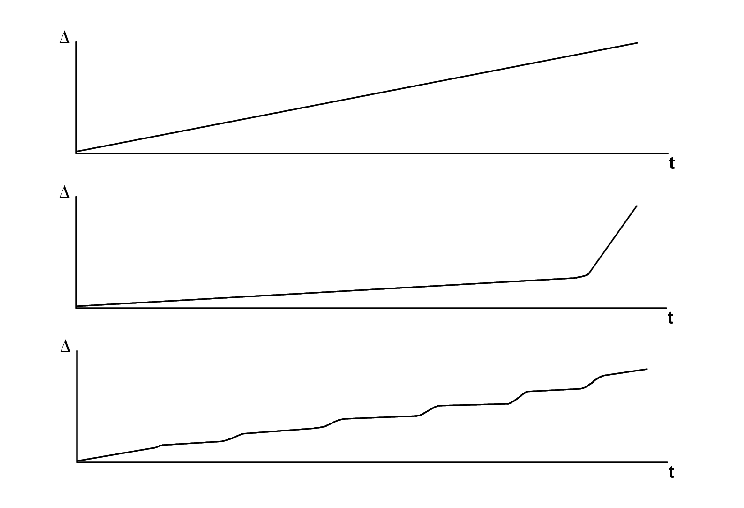
\includegraphics{pics/lgchggrph}
%     \caption{Three types of language change}
%     \label{fig:lgchangegraph}
% \end{figure}
% 
% Given the vicissitudes of the Malay history in Ceylon, a steady change does not seem probable.
% If there was a very abrupt language change, it must have been motivated by sociohistoric events of magnitude. One of these events is certainly the arrival of the first Malays in Ceylon, other possibilities are the eviction of the Dutch by the British, the disbandment of the Regiment and independence of Ceylon.
% 
% How likely was abrupt language change at these four points in time? The first settlers to arrive were exiles. Exiles do not leave their country of origin willingly. They prefer to stay in their homeland. The exiles (\em bannelingen\em) in Ceylon were insurgent leaders from the SEAA. They fought against Dutch rulership and for independence. As such, they are likely to value their own culture very highly. Furthermore, they hope to set again foot in their homelands. This makes them not very likely to innovate or adopt linguistic changes innovated by others.
% 
% The exiles were the Malay `elite' in Ceylon.  They numbered about
% 10\% of the population. At least they would not have undergone a
% major and abrupt linguistic change. They were serving as a
% guideline for the other groups, with whom they interacted. Some
% change is likely to have occurred, but not of a very abrupt
% nature.
% 
% The British takeover from the Dutch was rather smooth for the Malays, who quickly reassumed their old role as soldiers. The language of the military changed from Dutch to English. The two European languages being fairly similar in structure, and fairly remote from Malay or either Lankan language, a major impact of that is not to be expected.
% 
% The fading out and ultimate disbandment of the Regiment caused major distortions in Malay
% society. They lost their hearth in the Regiment, their social
% cohesion and many moved from  the garrison town to other places
% to find work. This changed the sociolinguistic setting in a more
% catastrophic way then the British takeover. With the
% sociolinguistic setting totally turned upside down, major repercussions on the language cannot be excluded.
% 
% \begin{quote}
% 	``networks chiefly constituted of strong ties support minority languages resisting institutional pressures to language shift; but when these networks weaken, language shift is likely to take place''\citep[124]{MilroyEtAl2003}
% \end{quote}
% 
% 
% Independence from the United Kingdom, nationalist movements and the promotion of the infamous ``Sinhala only'' law in 1956   \citep[35]{NissanEtAl1990} also had an impact on the sociolinguistic setting. School lessons were now in Sinhala, so the Malay children had to learn this language. They could no longer attend the English medium schools. On the other hand, English was still the language of economic ascendance. Many Malay families opted thus for English as the language spoken at the home to provide their children with good future opportunities \citep{Saldin2003}. This was to the disadvantage of Malay, and the source of language attrition that we observe today. Linguistic change in the post-colonial era was surely major, but not abrupt as it was only the younger generation that lost knowledge of Malay, while the parents still were in command of the language, but limited its use. Major Sinhala influence is likely to date from that period.
% 
% I conclude that no abrupt change happened at any of these four
% occasions (first settlement, British rule, disbandment of the
% regiment, independence.)
% 
% By exclusion of the first two possibilities, the change must have been gradual, with periods of heavy change alternating with periods of less change. The periods in which major changes are likely are the following:
%  
% \begin{enumerate}
%     \item the late 17$^{th}$ century: consolidation of a Lankan vehicular Malay
%     \item 1873+: dispersal of the community, loss of cohesion: major change
%     \item 1950+: forced introduction of Sinhala: major change
% \end{enumerate}
% 
% This view is supported in \citet{Ansaldo2005ms}.

 

\subsection{The linguistic ecology}
In Section \ref{sec:slmbg:SourcesintheSEAA} we have seen the diverse influences from the South East Asian varieties in different periods of history. In this section, I will briefly sketch the present linguistic ecology of Sri Lanka to shed light on which languages the Sri Lankan Malays encounter in their daily life.

The majority language of the island is Sinhala. Sinhala is a diglossic language \citep{Gair1968,
Gair1985diglossia,
Paolillo1992,
Paolillo1997},
with important differences between the high and the low variety. These differences cross-cut the spoken/written distinction, i.e. it is possible to combine high or low with spoken or written expression \citep{DeSilva1974,Gair1985diglossia,Paolillo1997}. The high variety is described by
\citet{Gunasekara1891},
\citet{Geiger1938,
Geiger1973},
and \citet{GairEtAl1974literary},
while the low variety is described by
\citet{Chater1815,
FairbanksEtAl1968,
Matzel1983,
GairEtAl1997,
Dissanayaka2003,
Jayawardena2004}
and \citet{Karunatillake2004}.
Linguistic analyses of various topics of Colloquial Sinhala are compiled in \citet{Gair1998} and \citet{Henadeerage2002}. The low variety is further divided between `Upcountry' and `Lowcountry' dialects, but the two are mutually comprehensible. The further dialectal subdivision is unclear and underresearched \citep[xii]{Jayawardena1996}. The descriptive material available for Colloquial Sinhala is  good and covers the speech of the groups the Malays have contact with.

The next biggest language of Sri Lanka is Tamil. While there is abundant literature on Tamil, it very often does not address the varieties relevant in the Sri Lankan context. Like Sinhala, Tamil is a diglossic language, with Literary Tamil being distinguished from diverse forms of Colloquial Tamil \citep{AnnamalaiEtAl1998}.  Colloquial Tamil can be divided into Indian Tamil and Sri Lankan Tamil. Spoken Indian Tamil is well described
\citep{Pope1867,
Arden1934,
Beythan1943,
Asher1982,
Lehmann1989,
Schiffman1999,
AsherEtAl2002,
AnnamalaiEtAl1998},
but differs from Sri Lankan varieties. Indian Tamil is present in Sri Lanka via media (television, films), and via the Estate Tamils, who came during the British period to work on the tea plantations. `Media Tamil' is quite homogeneous, but Estate Tamil is likely to still reflect the dialectal differences of the Indian immigrants from different regions of Southern India. The Malays do watch Tamil movies, and were in contact with Estate Tamils when they were overseers. This means that these two varieties of Indian Tamil can be considered as contact languages.

Dialectal variation in Tamil is underresearched \citep{Pillai1986}, especially in what concerns Sri Lanka.
\citet{Zvelebil1960,
Zvelebil1966}
distinguishes Jaffna Tamil, Trincomalee Tamil, Batticaloa Tamil and General Ceylon Tamil  on the basis of the phonology and morphology of a handful of speakers. \citet{Suseendirarajah1967,Suseendirarajah1973phon} adds some more description of the Tamil of Jaffna. The dialects of Jaffna and Trincomalee are not important for the analysis of SLM since the Malays had little contact with those towns.\footnote{There are some Malays in Trincomalee, but it is unclear whether they still speak Malay \citep[426]{Hussein2007}.} `General Ceylon Tamil' is more promising, as is Batticaloa Tamil \citep{Zvelebil1966, Suseendirarajah1973pron,Batticaloa}, with an important percentage of Muslim speakers. With the exception of Batticaloa, all these descriptions cover Hindu/Christian varieties. As for dialects on the other side of the island, \citet{Bonta2004,Bonta2008} argues that varieties of Negombo Tamil have converged towards Sinhala and have lost verb agreement.

The Moors have to be divided on sociological grounds into `Coast Moors' and `Ceylon Moors', of which the Ceylon Moors speak a Lankan variety while the Coast Moors, hailing from India, speak an Indian form of Tamil \citep[25]{Nuhman2007}, also discussed in \citet{Hussein2007}.
\citet[71ff]{Nuhman2007} distinguishes Sri Lanka Muslim Tamil from the Hindu/Christian varieties. He further divides North-Eastern Muslim Tamil from South-Western Muslim Tamil \citep[also see][45]{Hussein2007} and argues that verb agreement was lost in the South-Western variety as well. He furthermore gives an overview of some additional phonological, morphological and lexical characteristics of Muslim Tamil. To sum up, overall description of Tamil is very good, description of Sri Lankan Hindu/Christian Tamil is fair, and description of Muslim varieties is seriously wanting, as is a description of Estate Tamil varieties. Unfortunately, it is the Muslim and the Estate varieties which are especially interesting as contact languages for the Malays.

Another important language is, of course, English, in its Sri Lankan shape \citep{Kandiah1996}, while the  oldest inhabitants of Sri Lanka, the Veddah, and their language \citep{DeSilva1972}, have not been in extensive contact with the Malays.

\subsection{Heydays}
Different languages had different impact in different periods on the formation of SLM, as is common in contact language formation \citep{Arends1989,Roberts2004phd,Lim2007merger}. To go by chronological order, Portuguese was the first language to have the possibility to make an impact, although there is little evidence for that. The only item which could point to a Portuguese influence specific to Sri Lanka is \trs{salba}{escape}, which does not seem to exist in the SEAA. There are numerous other Portuguese words in SLM, but these are either also found in the SEAA (e.g. \trs{greeja/gereja}{church}) or in Sri Lanka (\trs{kusini}{kitchen}, Sinh. \em kussiya, \em Tam. \em kusini\em), so that it cannot be established that they were adopted in Sri Lanka during Portuguese rule. They might have entered the language later, through new immigrants bringing words like \em greeja \em from the SEAA, or through adstrate influence bringing words like \em kusini\em. After the Portuguese were ousted, their influence ceased. Next came the Dutch, who also failed to have a huge impact on the language. No Dutch word seems to be exclusive to SLM; they are all shared with other varieties of Malay and the local languages (like \trs{kaamar}{room}, Std. Malay \em kamar\em, Sinh. \em kaamaraya\em). During Dutch rule, many immigrants came from Java and other islands of the SEAA.
There is a strong trace of them in SLM, with 11,7\% of the vocabulary being traceable to them exclusively \citep{Paauw2004}. The influx from island immigrants ceased in 1819, and the immigration from peninsular Malays grew stronger. This new wave of immigrants, however, did not have an important impact. Only 0,6\% of SLM vocabulary can be traced to them \citep{Paauw2004}.
During the period of the regiment, Literary Malay was taught in the regiment schools, so  this language could have exerted influence on the spoken variety, although it is unclear whether this indeed materialized. When the regiment schools were closed, Malays switched to English education, and would cling to this medium of instruction until independence. English was probably already a major factor, but schooling in English increased the impact of this language from the late 19$^{th}$ century onwards. After Sinhala became the medium of instruction in government schools following independence, Sinhala increased its influence on SLM, and continues to do so up to today, due to the economic necessity to command this language.

As for Tamil, it is likely that it had an influence in the early days because many basic terms like \trs{kattil}{bed} are borrowed from this language, as are many names for animals. It is likely that the variety of Tamil was Muslim Tamil due to the shared religion; there is close to no evidence for prolonged contact with Hindu or Christian Tamils. The relative strength of Muslim Tamil influence over time is difficult to assess. In the beginning, when there were no Malay mosques, it was probably stronger, but as soon as Malay mosques were established and Malay life evolved around the military cantonments, Moor influence is likely to have decreased. The growing association with the Burghers and the adoption of a more intellectual and Westernized lifestyle in the 19$^{th}$ century suggest that the cultural ties between Malays and Moors became weaker in that period than what they had been before. But at the same time, the beginning of the estate economy, which employed many Malays as overseers over South Indian plantation workers, meant that the Malays had once again a good motivation to be conversant in Tamil. While the prestige of Estate Tamil was of course not very high, the relative size of labourers against overseers might have made up for that. As of today, the influence of Estate Tamil on Sri Lanka Malay (at least the Upcountry variety) remains understudied. With the orientation of Malays towards service economy, the contact with Estate Tamil decreased.

To sum up, most linguistic influence came, peaked and possibly disappeared. This is the case for the colonial languages as well as the languages of the immigrants, Estate Tamil and  Sinhala (which came to stay). An exception to this `peak' pattern is Muslim Tamil, which was probably present during the whole period in unclear proportions, possibly with a dip during the period of the regiment.

\subsection{Envoi: Against reductionism}
From the above descriptions, it should be clear that the linguistic history and ecology of Sri Lanka Malay are very complex. Sri Lanka Malay is definitely not a simple combination of Malay and Tamil and/or Sinhala. While this characterization could be used as a shorthand, it oversimplifies the diachronic complexities. To start with the immigrants, they surely spoke more than one language, and `Malay' is probably a misnomer to designate most of their varieties, if used without a qualification (Moluccan Malay, Jakartan Malay, Tangsi Malay etc.). It is not clear whether we can speak of `the immigrants' language' at all, given that the soldiers hailed from very diverse parts of the South East Asian Archipelago. Maybe there was a language which all of them shared, but it is more probable that that was not the case.\footnote{It should be borne in mind that Bahasa Indonesia, the national language of Indonesia, is a 20$^{th}$ century creation and is not spoken natively by a majority of the population \citep{Steinhauer2005}.} It is likely that different kinds of accommodations  were used on the part of a speaker to facilitate communication with addressees from different ethnolinguistic backgrounds, and that the `Malay lingua franca' was perpetually reinvented, very much like its Mediterranean counterpart \citep{Selbach2007,Selbachinpreparation}.

In Sri Lanka, Sinhala can be seen as a relatively homogeneous language. This is not the case for Tamil, where Hindu/Christian varieties and Muslim varieties differ considerably \citep{Nuhman2007}, and the especially interesting Muslim varieties show diatopic variation. Estate Tamil also differs from estate to estate depending on the origin of the workers. Just as we must ask `Which Malay?' when talking about the immigrants' language, we must ask `Which Tamil?' and `Which Sinhala?' when speaking about the language of the people they met in Sri Lanka.  Reconstruction of historical contact settings is notoriously difficult \citep{RenfrewEtAl2000,Lim2007merger,Ansaldo2009clfet}, but it is probable that the answers to these questions will not be `that Tamil' but rather `these Tamil varieties, those Malay varieties, those other Sinhala varieties'. Only when we have a full and precise picture of the input varieties, and the end product, will we be able to make solid analyses of the evolution of Sri Lanka Malay.

Diachronic language contact studies investigate the development of a new variety out of the contact between two or more prior varieties. The more information we have on the historical languages and the present day language, the more precisely we can trace the development of the language. As for Sri Lanka Malay, we have little information about the historical varieties, and not too much information about the current variety. While the Sinhala part seems OK, we need a better description of historical Trade Malay varieties,\footnote{After writing this chapter, I received a copy of \citet{Paauw2008phd}, which is a big step forward into that direction.} historical Muslim Tamil varieties, and present day Sri Lanka Malay to make solid analyses of the development of Sri Lanka Malay.
I will not be able to shed much light on the historical varieties in this thesis, but in the following chapters, I hope to advance our knowledge of the current shape of Sri Lanka Malay and  add the contemporary piece to the diachronic jigsaw puzzle.

\setcounter{exx}{0}\setcounter{footnote}{0}
	\chapter{Methodology}
\section{Theroretical assumptions}
The presentation in this grammar is intended to be as theory-neutral as possible. No knowledge of any particular theoretical framework is assumed in order to keep the book accessible for a maximum number of people, scholars and laymen alike. Theory-neutralness is also advisable with regard to future generations of linguists who might not be any more aware of the major linguistic trends in the beginning of the 21st century than we are aware of the formalisms of tagmemics that saw their heydays half a century ago.

Being theory-neutral does not mean that this grammar is atheoretical. There are many decisions in the presentation of the data that were guided by theoretical considerations. Structuring data is impossible without a solid theory that lays the fundament on which the grammatical findings can be grounded. But in a house, it is not necessary to see plans of the fundament in every room, and in a grammar book it is not necessary to cast everything into a powerful yet complicated formalism when it can also be said in simple, maximally theory-neutral words. The material for grounding this grammar on is mainly taken from Radical Construction Grammar \citep{Croft2001rcg} and Functional Discourse Grammar \citep{HengeveldEtAl2008fdg}. However, the reader will rarely notice this anymore than he notices the fundament of a house he happens to enter. Only on closer inspection of the architecture will he find signs of the fundament, e.g. in the specific disposition of pillars or chapters. Care has been taken to avoid theory-specific jargon and formalisms as much as possible. When formalisms are used, they are explained in detail. Normally, standard descriptive nomenclature has been used. Every nomenclature in itself relies on theoretical considerations, the nomenclature here is based on Basic Linguistic Theory \citet{Dryer2006blt, Dixon1997riseandfall}, which should be accessible to every reader with a basic knowledge of typology.

\section{Data collection}
The field work for this grammar was done in X field trips between november 2005 and 200X, of about 2 months each. During the trips, the focus was on data gathering, while the periods between them where devoted to analysis. The findings were cross-checked during the following field-trip. Focus was on natural discourse, monological as well as narration. In the first field trip, I did quite a lot of elicitation to get a feeling for the possible constructions in the languages so I could identify them when I heard/transcribed them. The phonological system is not very complicated and was already analyzed in the great lines \citep{Bichsel}, so I encountered little problems in deciding how to segment words or how to represent them orthographically. With a good preliminary orthography at hand, I was able to get into morphosyntax quite quickly. SLM has no complicated allophonic rules, and the set of allomorphs is also very restraint. This made it quite easy to segment morphemes and to identify the same morpheme in different contexts. From the first day on, I spoke as much Malay as possible\footnote{I have no command whatsoever of Standard Indonesian or Standard Malaysian. When I am talking of Malay in the following, Sri Lankan Malay is always intended.}. This was of course quite limited in the beginning, but my consultants got used to talking to me in Malay from the very beginnining. In this way, elicitation session were only a little different from normal interaction, and I hope this has taken away some of their artificial character.

The Malays all have a good command of English, so English was also used in conversation, not only for difficult topics, but also when the speakers just felt like it. In order to maintain a relaxed and casual atmosphere, I did not interfere with that. Maybe some day in the future a researcher wants to do research on code-switching and will be happy to have this material as is.

The examples in this book are mainly taken from natural discourse. For every example, its source is indicated. The source file follows certain conventions that permit to identify the text genre. The first letter indicates the town, the following number indicate the date (YYMMDD). The three following letters indicate the genre, for instance nar for narrative or eli for elicitation (see Table \ref{tab:genres} for a list). The transcriptions as well as the audio and possibly video files are available on the internet. The primacy of natural discourse over elicitation means that there are not many example that stem from an eli-file. These are mainly for negative judgments, which never occur in normal discourse, and marginal phenomena that could not be found in natural discourse but are generally considered of linguistic interest. A third reason to use elicited examples was the desire to keep the context constant, e.g. in the elicitation of paradigms.

\begin{table}
\begin{center}
% use packages: array,tabularx
\begin{tabular}{ll}
nar & narrative \\ 
cvs & conversation \\ 
sng & song \\ 
rcp & recipe \\ 
wrt & written text \\ 
prs & presentation \\ 
eml & email \\ 
\end{tabular}
\caption{Genre codes used in text examples}
\label{tab:genres}
\end{center}

\end{table}

\section{Data gathering techniques}
\subsection{Elicitation}
Elicitation. Let me be frank: I do not value elicitation very highly. The elicitor's wits, charm, subterfuge and creativity (or lack thereof) in making up contexts  determine a big deal more the grammaticality judgment of a given sentence than the consultant's intuition. Consultants like any other person you meet want the meeting to be enjoyable and one way of making it enjoyable is giving the linguist the things he wants to hear, or at least not refusing him the things he longs for that much. 
The linguist on the other hand might suppose that a certain construction would not exist anyway and not bother to check every context. After all there are many other things to be done that seem more promising, and time is limited.
This being said, a linguist is not interested in random sentences as they occur, but wants to investigate a certain topic and thus has to stimulate the informant to produce sentences that are of interest for the particular topic. Unfortunately, humans' intuition about their linguistic behaviour is mediocre \citep{Labov1975fact, datengwm}, so direct questions are best avoided.
One thing that surely triggers politeness and accomodation is the famous sentence \em Can you say X? \em I do not even talk about its variations like \em And you can't say Y, can you? \em and \em So you can also say Y? \em Of course people \em can \em say a lot of things. In the absence of schooling under prescriptive teachers, they can even say a lot more. There is a good lot of variation in many oral languages, and SLM is no exception. As such, speakers are used to a lot of variation in their input and will only reject a sentence if it seriously hinders comprehension. This grammar has the aim to provide an account of how Sri Lanka Malay is used. It is not an account of what people can be man\oe uvered into saying. Direct questions were thus only used as a technique of second language acquisition on the part of the researcher. If ever a grammatical phenomenon is illustrated by examples with \em eli \em in their source, caution should be exercised. It is very probable that the phenomenon under discussion is marginal and was only included for sake of completeness.

But how could specific grammatical phenomena be tested without direct questions? As a general principle, the methods involving less target language production by the linguist were preferred over others. The normal way of prompting informants to produce a certain sentence was to establish a certain context that would logically lead to an utterance with the desired meaning. When checking for specificational/identificational constructions for instance, the following context was presented: 

\ea Suppose you come home and you see that someone has broken in and stolen the TV, some money and so on. You do not know who that was. But later you learn that Farook was the thief. How would you then tell a friend that Farook was the thief? \z

Normally consultants would not just give the last sentence, but they would actually repeat the story with the final climax that Farook was found to be the thief. This sentence is \em Farook-jo maaling \em, with a focus clitic indicating that it is not a normal ascription.
Given that there was a whole story around, the consultants would not really know what I was looking at and could not really second-guess which information I was keen on and accomodate my desires.

If I suspected that there were other possibilities (I normally did), I asked precisely that.

\ea  Could you also say something else?  \z 

Note that this is already a greater commitment by the linguist because it suggests that there \em is \em something else, and consultants might try to be polite. If the construction I was looking for still did not show up, I would try to modify the sentence without revealing what my preferred structure would be. Something like 

\ea \ea Can you start with another word? \\
\\
 or \\
 
\ex Can you leave out something, and does that change the meaning? \z\z
 
come to mind. Still no target language material by the linguist. One step further is 

\ea Could you also start with X?\z

This involves production by the linguist, but it is very limited and the consultant still has to utter the sentence, instead of just nodding. Consultants easily accept doubtful sentences, but they rarely utter them themselves. The last level would be 

\ea And if I say X Y Z, how does that sound?\z

This last sentence is already pushing the linguist's production quite far and is susceptible to be accepted as correct even if no native speaker would ever utter it.
The second part of the sentence is crucial because the consultant cannot just say \em yes\em. She has to give a qualitative interpretation between something like \em very good \em and \em You can't say that. That does not mean anything! \em If the sentence X Y Z is accepted only at this late stage, it is mandatory to do two things. First, the consultant has to be asked to repeat the sentence. Many people can say that incomplete sentences are fine, for instance, but the dropped material will invariably show up when they are asked to repeat. The second thing is to ask which one of the sentences is `better', the one that the consultant gave first, or the one she finally accepted after direct prompt. The answer \em Yours is better \em clearly indicates politeness effects. Fortunately, I did not come across this. The answer \em both same \em is OK and indicates that there seems to be no great difference in acceptability between the two sentences. Still, it has to be noted down which sentence came first. The answer \em The second one is a bit odd, no? \em or \em You can say that in fast speech \em indicates that the second sentence would never be said in that way by the consultant and is thus ungrammatical.
A good technique is also starting the sentence in a doubtful tone and leaving it suspended in the middle, like looking for a word. Often, the consultant will join in then and finish the sentence.

One thing that is difficult with proceeding in this way is that it might lead to parrot responses at a certain point. With parrot responses I mean that the structure of the priming language is completely taken over in the target language. But prompting in the target language is worse as far as influence from the priming language is concerned because the linguist is very likely to impose certain structures of his language on the language he tries to describe. Be this as it may, consultants that would remarkably often copy the English order of constituents were asked some simple sentences in English and some comparable sentences in Sinhala, where the order of constituents is different from English. When their responses were like in English in the first case, but like in Sinhala in the second, this was ascribed to the parrot effect and caution was taken in interpreting these consultants' data. When the order of constituents remained consistent under different priming material, it was concluded that the given sentences were authentic.\footnote{
One remarkable feat in this domain is NH, who is not only able to repeat the same sentence with the same constituents a random number of times. Other people tend to replace NP by pronouns for instance, or offer alternatives. She is furthermore not influenced at all by the structure of the priming languages and will deliver very complex postverbal English subordinates invariably in preverbal position. All other informants would leave them as they are as they go along the sentence constituent for constituent.}

\subsection{Conversation and narratives}
While I tried not to speak SLM during elicitation sessions in order to not distort the data, I tried to avoid speaking English in conversation and when collecting narratives. People tend to give answers in the languages they are asked in, so asking in English would give stories in English, which was not desired. 

The inhabitants of Lanka are generally very sociable and love to chat. The Malays are no exception to this. They integrate foreigners very well, and so there is some linguistic production of mine to be found in the cvs-files. As far as I can see, this has not altered the speak of the Malays in general. I do not think that they accomodated their speech beyond reducing speed and articulating better (and even that they did not always do). I thus feel that examples from these conversations can be used to illustrate language use as well as any other file. In fact, the analysis of intonation is based on a conversation between several Malays and me where they inquire about my place of living etc. 

Sometimes my consultants would become involved in a conversation and forget about my presence. In that case, I often withdrew from the conversation and let them speak among themselves. These data are about the most naturalistic as one can get. Unfortunately, this is not only true for morphosyntax, intonation, discourse structure etc., but also for what is generally known as common ground. Given that I did not participate in the conversations, no need was felt to explain concepts and relations I was not aware of, and I must say that very often I had not the slightest clue what a conversation was about. This is partly due to specialized vocabulary, fast speech and so on, but also to the fact that I did not know the people, places and events that were interesting. Add this ignorance of the common ground to the general South Asian tendency to drop known material and you get a completely lost linguist.

Songs were also recorded, but the examples from there were not used to make points because songs often allow special constructions.
%  It might be interesting to do analyses of syllable structure and stress using songs \citep[cf.][]{Birch} but this has not been done yet.

\subsection{Translation}
The ``elicitation'' sessions were mostly spontaneous. I had noted down some phenomena I was interested  in and would improvise contexts for variations as we went along. However, sometimes I would use prefabricated English or Sinhala sentences to systematically check some phenomenon. 
Normally, I wrote up sentences for three or four different topics which I asked in random order. This was done to prevent entrenchment of the constructions. When people are asked the very same construction twenty times in a row with only marginal variation, they tend to rate the 21st construction like the others. Mixing in some completely different constructions can prevent this feeling of ``assembly chain elicitation''.

I also used examples from a learner's grammar of Spoken Sinhala\footnote{There are no textbooks for Spoken Sri Lanka Tamil.}\citep{Karunatillake2004}. This was done to see whether some categories that are grammaticalized in Sinhala are grammaticalized in SLM, too. For instance, I had the suspicion that SLM would have a grammaticalized evidential marker because this is an areal feature. However, asking to translate English sentences with some evidential reading like \em It is said/it seems that X \em would always yield \em arabiilang ...\em which is the lexical word ``to say''. It was impossible to construct a context in English where speakers were led to mark evidentiality. Using Sinhala primes proved an instant success, though. The Sinhala evidential clitic \em =lu \em in some sentence was translated as the particle \em kiyang\em. \em kiyang \em is the evidential marker that was impossible to elicit through English. Given this success, I copied all sentences from the learner's grammar and read them to the Malays, a source of big fun. From their translations, I could see whether there was some more grammaticalized material in SLM that was very difficult to elicit through English. Of course, this technique cannot be used as evidence for semantics or word order because of interference effects. Where it can be used succesfully is to establish the existence of spurious grammatical morphemes.


\subsection{Word lists}
Word collection was largely done in a spontaneous and associative way. Swadesh lists and extended Swadesh lists for South Asia taken from \citet{Abbi2001} were also used. Abbi also provides questionnaires for some typical areal phenomena, but it was found that they were too schematic and would not yield good responses.

Every now and then, I checked parts of my dictionary with consultants to see whether I had correctly written down what they had told me. This was especially necessary for the different coronal stops. I found it very hard to hear the difference between dental and alveolar stops (the latter are allophones of retroflex stops), so cross checking was necessary. The Sinhala alphabet has different graphemes for each one of these stops, so I could ask the consultants to write down the Malay word in Sinhala script and see which grapheme they would use\footnote{Sri Lanka has a literacy rate of 95\%, and the Malays are among the best educated ethnic groups so this technique is culturally adequate. Also, the Sinhala alphabet is phonemic and the pronounciation of a given grapheme is always predictable. My informants happened to be more familiar with the Sinhala script, but the Tamil script could also have been used.} 
This method relies on writing because when asked which letter they would write, they would either say \phonet{\dentt aj@n@} or \phonet{\tz aj@n@}, the Sinhala names of the letters. This leaves the initial problem of whether the stop was dental or alveolar. But \phonet{\dentt aj@n@} is represented in Latin script by \graphem{th}, so I found out that I could ask the informants whether a certain word should be spelled with \graphem{t} or \graphem{th}. The answer would indicate whether the stop was dental (th) or alveolar (t).
Other contexts where this asking to write down a word was useful was vowel quantity, the presence or absence of a labial approximant before [u] and the distinction between prenasalized consonants and combinations of nasal+homorganic stop.

\section{Recording}
\subsection{Primary recording}
Most sessions were recorded on audio with permission of the consultants. Sensitive material was deleted on request or not recorded. Recording devices are a bit obtrusive, and speakers were a bit uneasy at first. I have the impression that after some time the consultants got used to the recording device and continued talking like normal.

Some sessions were also recorded on video with a very small camcorder. This is more obtrusive than audio recording, and the data are less naturalistic. Some people were perfectly fine with being taped while others seemed to be a bit uneasy. In the latter case, the video camera was not used much. I found that using a tripod improves the technical quality, but decreases the linguistic quality of the data because people tend to fix the camera. This is why I did not use it much. I would normally sit with the camera on my lap, the LCD display turned 45^{o} so I could see it. This permitted to keep eye contact with the consultant and to use mimics and gesture to signal that I was keeping track of the story. At the same time, I could occasionally shed a glance to the LCD to see how the camera was doing, whether the tape was full or the battery empty etc.

All audio data were recorded as linear pcm at 44,1kHz on flash memory cards using a Mayah Flashman ZXCVBNM and a SONY QWER microphone. Video was taken with a SONY ASDFG and a gun microphone. The videos seen in the archive have their audio track replaced by the Flashman audio track because the latter's quality is superior.

\subsection{Postprocessing}
Every evening, the audio data were copied to the laptop, and video was captured with the program Premiere. Video was converted to mpeg1 and mpeg2 with the program Tsunami\footnote{It is a somewhat awkward feeling to use a program called Tsunami in Sri Lanka on an everyday basis.}, while audio was left as pcm/wav. The audio files were segmented into thematic chunks with the program transcriber and cut into smaller sesion files with the export function of the same program. Mpeg1, mpeg2, master audio files and session files were stored in a folder that was burnt on two DVDs when it reached 4 GB. One DVD was sent by snail mail to Amsterdam while the other DVD served as a local backup. 

The data collected during one trip amount to about 50 GB, which is too much for my laptop's hard disk. An external USB-disk was used for extra storing capacity. This disk was also used as an additional backup place as long as space permitted.

The very first narrow phonetic transcriptions were done using transcriber. I wanted to use the program Keyman, which permits easy insertion of IPA symbols into any program. But I had to find that Keyman and transcriber would not work together. I finally used transcriber as if keyman worked. This means for instance typing e= to get a schwa. In any other program, the conversion is done instantly, but not in transcriber. I stored the file with e= and later search\&replaced the e= by \E. After I had worked out an orthography, this was no longer necessary because the orthography only draws on the standard latin alphabet.

Transcriptions were also backed up on the same DVDs as the media files. I wrote a small perl script to convert the transcriber files into Toolbox files, keeping the time code information in a way that ELAN would later be able to import my Toolbox files. Toolbox was used to interlinearize the transcriptions. As a final step, the Toolbox file was imported into ELAN and aligned with video if that was available (the audio file was already aligned through the time code I had kept).
\setcounter{exx}{0}\setcounter{footnote}{0}
  \part{Form}
	
\chapter{Phonology}
\glossSTDmode
Phonological research on Sri Lanka Malay started out with a Bachelor's thesis \citep{Tapovanaye1986} and two Master's theses    \citep{Bichsel, Tapovanaye1995}. It thus predates research on other areas, but then the domain lay dormant and most subsequent research concentrated on morphosyntax, although \citet{SmithEtAl2004} contains some analyses of phonological influence from Muslim Tamil.\footnote{Bichsel-Stettler worked with informants  from the Colombo-Gampaha area during about 14 months. Tapovanaye is Sri Lankan, and worked with Malays from the Colombo area as well, mainly in elicitation settings. The data in \citet{SmithEtAl2004} come from a transcript of about 500 sentences taken from a recording  made in the Southern village of Kirinda in the late 1970s.} According to \citet{Ansaldo2005ms} ``phonology of [SLM] varieties is the least understood aspect.''
This chapter will first present the segmental inventory consisting of 6 vowels and 24 consonants (including 2 glides), and then proceed to the suprasegmental domains of syllable structure, word structure, and sentence intonation.


\section{Segments}\label{sec:phon:Segments}
\glossIPAmode
This section  introduces the segments of SLM phonology.\footnote{I would like to thank Wolgang Kehrein and Diana Apoussidou for help with this section. They have corrected many of my oversights and set right my misconceptions about certain parts of phonology. All remaining errors are entirely my own.}
 Until the presentation of the practical orthography in Section \ref{sec:phon:Orthography}, all examples are in broad phonetic transcription following the IPA alphabet.

\subsection{Vowels}\label{sec:phon:Vowels}
The SLM vowel system consists of five full vowels and schwa. It is thus the same as that of colloquial Indonesian \citep[229]{Ewing2005} and many Malay varieties in general \citep{Adelaar1985,Adelaar2005struct}. 

\begin{table}[!h]
    \centering
        \begin{tabular}{rccccc}
        %            & front &   & central &   & back \\
                &  i    &  	 &        	 &  		 &   u   \\
                &       &  e &  \textipa{@}       &  o &      \\
                &       &   &    a   &   &      \\
        \end{tabular}
    \caption{SLM vowel phonemes}
    \label{tab:SLMVowelPhonemcdes}
\end{table}

The near minimal pairs in \xref{ex:phon:vowels:minimalpairs} illustrate the distinctions between the full vowels.


\xbox{14}{
\ea \label{ex:phon:vowels:minimalpairs}
\gll pa\dentn\dentt as pre\dentn\dentt a bi\dentn\dentt an o\dentn\dentt a bu\dentn\dentt ur  \\
     hot law star camel knock  \\
\z
} \\
% 
% A more systematic comparison is given below.
% 
% \subsubsection{Vowel contrasts}\label{sec:phon:Vowelcontrasts}
% 
% \paragraph{High vs. mid}
% ~
% 
% \xbox{7}{
% \ea 
% \gll p\textbf{i}\dentn\dentt u --- pr\textbf{e}\dentn\dentt a \\
%       door --- law \\
% \z
% } 
% \xbox{7}{
% \ea 
% \gll kumba\ng{} --- p\textbf{o}mpa\ng{}  \\
%      flower --- female  \\
% \z
% } \\
% 
% 
% \paragraph{Mid vs. low}
% ~
% 
% \xbox{7}{
% \ea 
% \gll pr\textbf{e}\dentn\dentt a --- p\textbf{a}\dentn\dentt as\\
%      law --- beautiful       \\
% \z
% } 
% \xbox{7}{
% \ea 
% \gll  kamp\textbf{o}\ng{} ---  gamp\textbf{a}\ng \\
%       village --- easy \\
% \z
% } \\
% 
% 
% \paragraph{Front vs. back}
% ~
% 
% \xbox{7}{
% \ea 
% \gll p\textbf{i}\dentn\dentt u --- b\textbf{u}\dentn\dentt ur  \\
%       door --- knock \\
% \z
% } 
% \xbox{7}{
% \ea 
% \gll l\textbf{e}mpas --- l\textbf{o}mpa\dentt   \\
%      toss --- jump  \\
% \z
% } \\




% \parbox{8cm}{
% \ea
% \gll \textipa{ka:ki} --- \textipa{ka:kE} \\
%      `leg' --- `grandfather'\\
% \z
% }
% \parbox{6cm}{
% \ea
% \gll \textipa{bu:la\dentt} --- \textipa{bO:lE} \\
%      `whole' --- `CAN'\\
% \z
% }\\
% 

% ~
% 
% \parbox{8cm}{
% \ea
% \gll \textipa{ka:kE} --- \textipa{ka:ka} \\
%      `grandfather' --- `elder.brother'\\
% \z
% }
% \parbox{6cm}{
% \ea
% \gll \textipa{bO:lE} --- \textipa{ba:lEk} \\
%      `CAN' --- `turn\\
% \z
% }
% 
% ~
% 
% \parbox{8cm}{
% \ea
% \gll \textipa{ci:ci} --- \textipa{cu:cu} \\
%      `great.grandchild' --- `grandchild\\
% \z
% }
% \parbox{6cm}{
% \ea
% \gll \textipa{bE:bEk} --- \textipa{bO:\dz Ok} \\
%      `duck' --- `spoilt\\
% \z
% }
% 



\paragraph{Schwa}
There is one centralized vowel in SLM, which can be realized as [\E], [\I], [\U], [i] or [u], depending on context. These contexts will be dealt with in more detail below. I will refer to this phoneme as `schwa', without committing myself to any particular realization. The following examples show schwa in its realization as \phonet{@} contrasting with \phonet{a} in \xref{ex:phon:schwafin1} and schwa in its realization as \phonet{I} contrasting with \phonet{i} in \xref{ex:phon:mEnthamintha}.


\xbox{7}{
\ea\label{ex:phon:schwafin1}
\gll ka\dentt:\E m --- ki\dentt am \\
    almsgiving        --- 1\textsc{pl}  \\
\z      
}
\xbox{7}{
\ea\label{ex:phon:mEnthamintha}
\gll m\I \dentn\dentt a ---  mi\dentn\dentt a \\
    vomit ---      ask \\
\z      
}

There are some speakers who do not have reduced vowels on the surface. These speakers will pronounce both words in \xref{ex:phon:mEnthamintha} \phonet{mi\dentn\dentt a} and consider them homophonous.\footnote{SLM
 behaves like many other Austronesian languages in this regard, where the status of schwa is often difficult to determine \citep[116]{Himmelmann2005typochar}.}
Other phonological effects triggered by schwa, like gemination (see Section \ref{sec:phon:Analysisofwordstructure}) are not affected by this homophony.
Speakers who do make the distinction have clearly different formants for realizations of /i/ as [i] and realizations of /\E/ as \phonet{I}, as shown in Figure \ref{fig:minthamEntha}

\begin{figure}
 \centering
 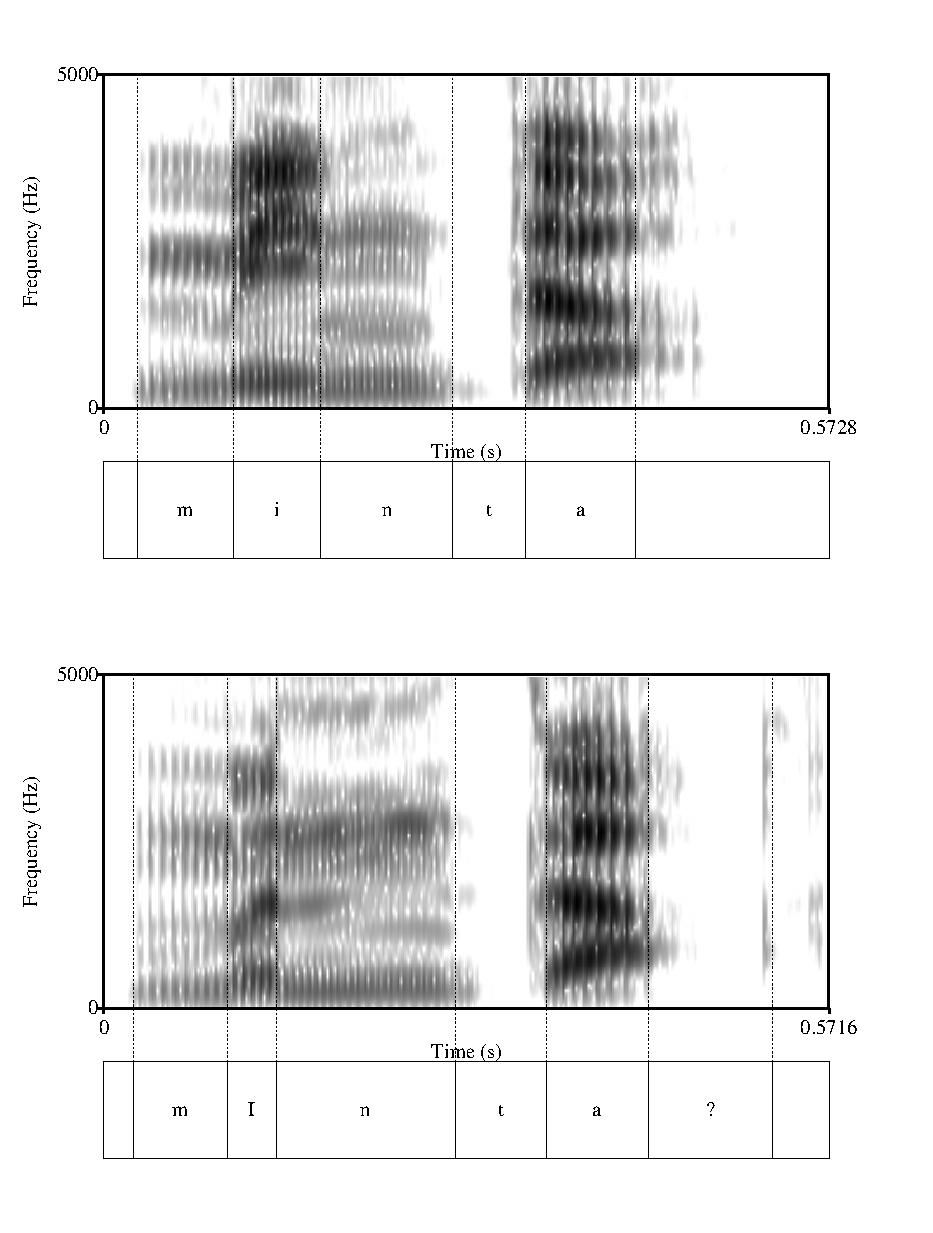
\includegraphics[width=.8\textwidth]{pics/minthamEntha.eps}
 % mentaminta.eps: 32x24 pixel, 0dpi, 70819821227670020548853019185250304.00x53114867158692554697020039288061952.00 cm, bb=
\caption[Formant structures for \phonet{I} and \phonet{i}]{The formant structures of the first vowels in \phontrs{mi\dentn\dentt a}{ask} and \phontrs{mI\dentn\dentt a}{raw} are clearly different, indicating that /i/ and /\E/ are different phonemes, which distinguish the two meanings. The second spectrogram indicates a glottal stop after the final vowel. This is not phonemic, as will be discussed in more detail below (Section \ref{sec:phon:Consonants}). }
\label{fig:minthamEntha}
\end{figure}



% The different realizations of schwa are discussed in more detail below (Section \ref{sec:phon:Majorallophonesofschwa}).



\subsubsection{Major  allophones of the full vowels}\label{sec:phon:Majorallophonesofthefullvowels}
The vowels /a/ /i/ and /u/ are always realized as full vowels. /e/ and /o/ can be realized as lax  \phonet{E,O} or tense \phonet{e,o}. Tense realizations are more often found in open syllables.

% \begin{figure}
% 	\centering
% 		\vspace{6cm}\includegraphics{pics/seelong.eps}\vspace{0.5cm}
% 	\caption{The first occurrence of the word for ``Ceylon'' is with a tense [e] the second one with a lax [\ipaE]}
% 	\label{fig:phon:seelong}
% 	%K051222nar04
% \end{figure}



 In  some words, the pronunciation of /e/ approximates the pronunciation of /i/ in the same contexts, e.g. /\dentt ekus/, `mouse',\footnote{Vowel length is not phonemic, as will be discussed in Section \ref{sec:phon:Vowellength} and therefore not indicated in the phonemic notation.}  is pronounced as [\dentt\textlowering{i}:kus].


\subsubsection{Major  allophones of schwa}\label{sec:phon:Majorallophonesofschwa}
The realization of schwa depends on its position within the stem and on the individual speaker. Schwa can be realized as \phonet{I,@,U}, and sometimes even as \phonet{i,u} (cf. \citet[27f]{Adelaar1991}, \citet{SmithEtAl2004}).


\paragraph{Variations in height}
In the final syllable, schwa is realized as \phonet{@} or \phonet{a}, depending on the speaker. In the penultimate syllable, schwa is raised by all speakers (e.g. \phontrs{bIs:aR}{big}). The amount of raising depends on the speakers. Some speakers raise to \phonet{I} or \phonet{U}, which makes the identification of the sound as a centralized vowel easy. Other speakers raise the vowel further, to \phonet{i} or \phonet{u}. In that case, the question  whether the sound is underlyingly schwa or a full vowel can only be answered by looking at word structure (see Section \ref{sec:phon:Analysisofwordstructure}). Especially a following geminate is indicative of the sound being schwa on the phonological level. In the antepenultimate and before, schwa is always realized as \phonet{@}. An example is \phontrs{c@ca\V ak}{wash}.\footnote{The normal word for `to wash' is \phonet{cu:ci}; `to bathe' is \phonet{man\postalvd i}. \phonet{c@ca\V ak} refers to an activity known in Sri Lanka as `body-wash'. This reflects the etymology of \trs{*cuci+awak}{body+wash}. I will use `wash' in the gloss as a shorthand.}

No trisyllable can have \phonet{I,U} in the initial syllable. A first set of trisyllables bans raising altogether in the initial syllable, while a second set requires raising to \phonet{i,u}. Neither set admits alternation between schwa and a high vowel. Examples for the first set are
\phontrs{c@ca:\V ak}{body wash},
\phontrs{b@Rna:ma}{famous},
\phontrs{m(@)la:ju}{Malay}, while an example for the second set is \phonem{k\E mare\ng} $\to$ \phonet{kuma:Re\ng} `yesterday'.

Since no reduced vowel is possible in the second set, contrary to the disyllables like \phontrs{\dentt\{\U/u\}l:Or}{egg},  the question arises why a schwa should be present in the underlying form. The reasons for this have to do with syllable structure and the lengthening of the vowel and will be discussed in more detail in Section \ref{sec:phon:Analysisofwordstructure}.


The verbal prefixes \phontrs{aR\E-}{\textsc{non.past}},\footnote{The semantics of this prefix are more complicated than what can be capture in the gloss here, the reader is referred to Section \ref{sec:morph:ara-} for a more thorough discussion of this prefix.}
\phontrs{an\E-}{\textsc{past}} and \phontrs{m\E-}{\textsc{inf-}}\footnote{And some other much less common prefixes, see Section \ref{sec:morph:Prefixes}.} have an unraised schwa [\E] irrespective of the syllable position. Given that most roots are disyllabic,  schwa is normally in antepenultimate position as in \phontrs{aR\E-ma:ka\ng}{is eating}, \phontrs{an\E-mi:nu\ng}{drank}, \phontrs{m\E-\J a:la\ng}{to go}, but it can also be found farther away from the end, as in \phontrs{aR\E-c\E ca:\V ak}{is washing}.  There is only one monosyllabic verbal root \phontrs{pi:}{go}. The prefixes keep the schwa unraised when combined with this root, even if this results in \phonet{\E} being in penultimate position (where normally only \phonet{I} or \phonet{U} are found): \phonet{aR\E-pi:, an\E-pi:, m\E-pi:,*aRI-pi:, *anI-pi:, mI-pi:}. Evidence from vowel lengthening suggests that these prefixes do not form one phonological word with the verb. This means that the realization of schwa in these prefixes is independent of the structure of the verb the prefixes attach to.



\paragraph{Fronting and retracting}\label{sec:phon:allophonesofschwa:frontingandretracting}

Whether schwa is raised to a front vowel \phonet{I,i} or to a back vowel \phonet{U,u}  seems to be lexically determined, but there are some phonological cues. Some lexemes only admit a front vowel, some only a back vowel, some accept both. The following list gives examples.

\ea \phonem{@mpa\dentt} `four' $\to$\phonet{Umpa\dentt}. Further raise:  \phonet{umpa\dentt}\z
\ea \phonem{g@lap} `dark' $\to$\phonet{gIl:ap}. Further raise:  \phonet{gil:ap}\z
\ea \phonem{\dentt@lOr} `egg' $\to$\phonet{\dentt Il:OR} or \phonet{\dentt Ul:OR}. Further raise:  \phonet{\dentt il:OR} or \phonet{\dentt ul:OR}\z
\ea \phonem{p@laN} `slow' $\to$\phonet{pIl:aN} or \phonet{pUl:aN}. Further raise:  \phonet{pil:aN} or \phonet{pul:aN}\z

From this list and additional material it appears that two factors have an influence: the following consonant and vowel harmony. A back vowel is most often found before a labial consonant /p,b,m/
\phontrs{d\U p:a\ng}{front},
\phontrs{k\U b:o\ng}{garden},
\phontrs{\U m:a}{mother} \citep[cf. ][27]{Adelaar1991}. Dorsal consonants seem to favor a front vowel:
\phontrs{sIg:aR}{healthy},
\phontrs{dIk:a\dentt}{vicinity}.\footnote{For theoretical discussions of this, see \citet{Clements1990sonority} and \citet[99]{Botma2004}.}
For the other consonants, a clear pattern could not be found.

\citet{Bichsel} found vowel harmony in words like \phontrs{lib:i}{more} and \phontrs{g\U m:uk}{fat} \citep[also cf.][27]{Adelaar1991}.
The schwa in the initial syllable is raised and agrees in the feature [$\pm$back] with the following vowel.

All this being said, there seems to be a lot of variation between and even within dialects. In the text K060103rec02 for example, the word for `raw' was transcribed by a native speaker once as \graphem{mintha} and two sentences later as \graphem{muntha}. Notwithstanding the intended and actual realization by the speaker, this proves that for the hearer/transcriber in this case, both the rendering of the first vowel as \graphem{i} and as \graphem{u} were acceptable, suggesting that the phonological knowledge of the hearer has no strict distinction between the fronted and the retracted realization.



\paragraph{Deletion}\label{sec:phon:schwa:deletion}
In the initial syllable of di- and trisyllables, schwa is often dropped if the resulting sequence is phonotactically acceptable.\footnote{Jakarta varieties of Indonesian show frequent deletion of schwa in initial position (Uri Tadmor p.c., \citet[229]{Ewing2005}) Many of the Sri Lankan Malays came from/through Jakarta, so that this could very well be an inherited feature.} An example for this is \phonet{m(@)la:ju} `Malay', which is rarely heard with the schwa pronounced; it is much more common to have the sequence \em ml \em as the onset of the first syllable (\phonet{mla:.ju}). Schwa is not dropped in \phontrs{c@ca:wak}{wash} and \phontrs{b@Rna:ma}{famous} because the sequences \em \#cc(c\textipa{:}) \em and \em \#brn \em are not acceptable phonotactically. Deletion of schwa is also found in disyllables,  such as \phonem{b@ras}`rice', which can be realized as \phonet{br:as}, next to \phonet{bIr:as}.\footnote{The realization with \phonet{i} is never found for this lexeme.} This reduction of schwa can also take place if no onset is present: \phonem{@ma}`mother' can be realized as \phonet{Um:a}, \phonet{um:a}, or  \phonet{\s{m}ma} with a syllabic nasal.

Realizations like \phonet{b(I)r:as}`rice' or \phonet{p(I)r:a\ng}`war' raise the question whether schwa is present in the phonological form, and then deleted, or whether it is absent in the phonological form and then  epenthetically inserted.\footnote{Tamil for instance has epenthetical insertion of \phonet{I} in onset clusters like \trs{viyaaparam}{business}$<$Skrt. \em vyaabhara \em \citep[103]{AnnamalaiEtAl1998}.} There are two reasons to prefer the deletion account over the epenthesis account. First, there is a phoneme schwa anyway, so the presence of schwa in this position is no additional burden. Second, schwa varies with \zero{} only in some contexts, in lexemes like \phontrs{c\E ca:\V ak}{wash}, \zero{} is not possible. An epenthetic account can thus not explain the whole story, while the deletion account can. Additionally, schwa is the historical vowel in these words, although the speakers are of course not necessarily aware of this.



\subsubsection{Vowel length}\label{sec:phon:Vowellength}
Full vowels are predictably lengthened in open penultimate syllables.  Long vowels are not found in other positions. Vowel length is thus not phonemic (\em contra \em \citet{Bichsel, SmithEtAl2004}), but conditioned by nature and position of the syllable \citep[cf.][]{Tapovanaye1995}. Example \xref{ex:phon:vowellength} shows this lengthening process for all full vowels.


\xbox{14}{
\ea \label{ex:phon:vowellength}
\gll ma:Ra --- me:Ra --- \postalvd i:Ri --- so:Re --- mu:Ra  \\
      anger --- red --- body --- evening --- cheap \\
\z
} \\

Example \xref{ex:phon:vowellength} contains only disyllabic words.
In trisyllabic words with an open penultimate syllable, the syllable is lengthened if the initial syllable contains a schwa \xref{ex:phon:vowellength:trisyl:schwa} in any of its realizations (\phonet{@,I,i,U,u}). It is not lengthened otherwise \xref{ex:phon:vowellength:trisyl:noschwa}.\footnote{There are close to no underived stems without schwa in the initial syllable. I analyze \phontrs{nigiri}{country} and \phontrs{ku\dentt umuN}{see} as having no schwa synchronically in spite of the diachronic origins \em n\E g\E ri \em and \em k\E t\E mu \em because the vowels are always pronounced as full vowels, and none of the other phonological effects of schwa are found. As far as trisyllabic words derived with affixes go (like \em makan-an\em), all have only short vowels.}


\xbox{14}{
\ea \label{ex:phon:vowellength:trisyl:schwa}
\gll c\E ca:\V ak --- m\E la:ju  --- kuma:Re\ng   \\
      wash  ---  Malay ---  yesterday\\
\z
} 


\xbox{14}{
\ea\label{ex:phon:vowellength:trisyl:noschwa}
\gll nigiRi ---  ku\dentt umu\ng{} ---  makanan \\
     country  --- see ---  food  \\
\z
} \\

No surface form of an underlying schwa (\phonet{@,I,i,U,u}) is ever lengthened. Instead, often another phonological process, consonant gemination, takes place, see Section \ref{sec:phon:Analysisofwordstructure}.

This general pattern is very regular throughout the grammar, but a certain number of exceptions apply:

\begin{itemize}
 \item function words never have long vowels: \phontrs{ki(*:)\dentt am}{\textsc{1pl}}, \phontrs{ka(*:)\dentt a}{\textsc{quot}}, with the exception of interrogative pronouns.
\item the sequence V$_i$hV$_i$ never has a long vowel: \phontrs{le(*:)heR}{neck}, but \phontrs{la*(:)heR}{be.born}
\item some sequences VGV, where G is a glide, have a long vowel, others do not. \phontrs{\dentt u*(:)\V a}{old}, \phontrs{\dentt u(*:)\V an}{Sir}. See Section \ref{sec:phon:nonphonemicglideformation} for detailed discussion.
\item the sequence \em uru \em has no long vowel in the words \phontrs{\dentt uRus}{straight}  and \phontrs{guRu}{teacher} (but there is a long vowel in  \phontrs{ku:Rus}{thin}).
\item two words are lexical exceptions \phontrs{kubu:R}{bury}{} and \phontrs{ka:R\dentt u}{quarter}. The former has a long vowel in the final, not the penultimate, syllable. The latter has a long vowel in the penultimate syllable, but the syllable is not open.
\item Loanwords from English and Arabic tend to violate this pattern.
\end{itemize}


 

\subsubsection{Distribution of the vowels}\label{sec:phon:Distributionofthevowels}
For the discussion of the distribution of vowels, we distinguish the root level from the stem level. In the context of this discussion, roots are defined as monomorphemic lexemes, while stems consist of at least one root and optional additional morphemes, lexical or derivational. To illustrate the distinction with English examples, \em farm \em would be a root,\footnote{And also a stem.} whereas \em dairy farm \em or \em farmer \em would be stems, because they comprise additional morphemes, \em dairy \em and \em -er \em in these cases.

In SLM roots, there are no restrictions for the final and the penultimate syllable. Here, all vowels can be found. Examples are given in Table \ref{tab:vowelpositions}. In the antepenultimate position, only [i], [u] and [\E] are found in native roots. Any vowel can be found in the antepenultimate position in loanwords, which are given in parentheses in Table \ref{tab:vowelpositions}.

\begin{table}
	\begin{center}
		\begin{tabular}{llll}
		& antepenultimate& penultimate & final \\
		\hline
		a & (\textipa{va\tz:ak:a:}`pumpkin', Tamil)	& \textipa{\dentt aksiR} `think'	& \textipa{kap:al} `ship' \\
		e & (\textipa{selin\postalvd i}`{spider}', Tamil)	& \textipa{seksa} `problem' 	& \textipa{slampe} `handkerchief'\\
		i & \textipa{nigiRi}`country'	& \textipa{mi\dentn\dentt a} `ask'& \textipa{sampi} `cow'\\
		o & (\textipa{goRaka:}`a condiment' Sinhala)	& \textipa{pompa\ng} `female'	& \textipa{na\dentn\dentt ok} `sleepy' \\
		u & \textipa{ku\dentt umu\ng}`see'	& \textipa{kumba\ng} `flower'&	 \textipa{campuR} `mix'\\
		schwa & \textipa{c\E ca\V ak} `wash'	& \textipa{mI\dentn\dentt a} `vomit'	& ka\dentt:\E m `almsgiving'\\
		\end{tabular}
		\caption[Vowels in different positions within the root]{Vowels in antepenultimate, penultimate and final position of roots. In antepenultimate position, a, e and o are only found in loanwords, indicated by parentheses. The word \trs{bahasa}{language} could be an exception, but this seems to be a recent borrowing from Standard Malay, the native word is \phonet{ba:sa}.}
		\label{tab:vowelpositions}
	\end{center}
\end{table}

As for stems, no such restrictions apply. When adding the nominalizing suffix \em -an \em to a verbal root, the penultimate becomes the antepenultimate and keeps its vowel. In this way, [e], [o] and [a] can be found in the antepenultimate, e.g. \phontrs{pake-yan}{dress\textsc{-nmlzr}},\phontrs{po\dentt o\ng-an}{cut-\textsc{nmlzr}}, \phontrs{pegan- an}{catch-\textsc{nmlzr}}. Similar things can be said about compounding, which also shifts syllables farther away from the right edge. This does not affect the occurrence of [e], [o] or  [a] either. Examples are \phontrs{oRa\ng{} ik:a\ng}{man+fish=fisherman}  and \phontrs{babi u:\dentt a\ng}{pig+forest=wild boar}.

While schwa can occur anywhere, it is most often found in the penultimate and the antepenultimate. There are only two occurrences of schwa in the final syllable of two words, which are given below

\xbox{7}{
\ea\label{ex:phon:schwafin:thaanEm} 
\gll \dentt a:n\E{}m\footnotemark{} \\
    `plant(V)' \\
\z
}
\xbox{7}{
\ea
\gll ka\dentt:\E m \\
    `almsgiving' \\
\z
}
\footnotetext{While Std. Malay does not permit schwa in the final syllable, Jakartanese does \citep{AdelaarEtAl1996}, and \em tan\E m \em is also found in that variety, with the same meaning \citep[200]{Adelaar1985}.}

\subsection{Consonants}\label{sec:phon:Consonants}
SLM numbers 24 native consonants and glides plus 3 consonants only used for loanwords. 5 basic places of articulation are distinguished for stops: labial, dental, apical (with postalveolar and retroflex allophones),\footnote{I use `apical' as a cover term for  postalveolar and retroflex realizations. This term as it is used here never includes the dentals, no matter how they are realized.} palatal, and velar. These places have a series of voiceless stops, voiced stops and prenasalized voiced stops.\footnote{The dental prenasalized stop is missing.} The palatal stops are realized as affricates (For the general treatment of affricates as strident stops see \citet{JakobsonEtAl1952speechanalysis,Clements1999affr}, and \citet{Kehrein2002affr}.
% \footnote{As is the case with most other languages on the subcontinent,  languages which have palatal affricates do not have palatal stops. \citep[67]{Ramaswami1999}.}

All stops are matched by homorganic nasals, with the exception of the lamino-dental nasal, which does occur phonetically, but lacks phonemic status.

The fricative series is less populated, with /s/ being the only fricative frequently encountered. There are some words with /h/, but overall /h/ is much less frequent than /s/. /f/, /z/ and /\sh/ are finally only found in loanwords from Arabic (\phontrs{zihaRa\dentt}{shrine}) or English (\phontrs{femili}{family}, \phontrs{bRItIS}{British}). /f/ and /z/ are also found in many Islamic names like \em Farzan \em or \em Fayizal\em.

/l/ is an alveolar lateral approximant. /r/ is a rhotic realized as a tap or a trill.

The picture is completed by a labiodental approximant \V{} and a palatal approximant \textipa{j} (cf. Table \ref{tab:SLMConsonantPhonemes}).

\begin{table}
    \centering
        \begin{tabular}{lcccccc}
                 & labial & dental & apical    & palatal          & velar & glottal\\
        \hline
        stops    &&&&&&\\
        ~~~voiceless& p   & \dentt{} & t        &    c        & k   &   \\
        ~~~voiced   & b   & \dentd{} & d        &   \J          & g   &   \\
	~~~prenasalized&\mb& 	     & \nd         &  \nJ        & \nG &   \\
	nasals      & m   &         &  n           & \ny	  & \ng &   \\
       fricatives  & (f) &          &    s (z) (\textesh)    &   &     & h \\
	 approximants & \V  &          &       &   j         &     &   \\
	 liquids &   &          &  r ~~ l      &            &     &   \\
        \end{tabular}
    \caption[SLM consonant phonemes]{SLM consonant phonemes, including approximants. Palatal stops are phonetically affricated. Parentheses indicate phonemes only found in loanwords.}
    \label{tab:SLMConsonantPhonemes}
\end{table}
% 
% 
% \begin{figure}
% 	\centering
% 	\subfigure[Sinhala consonant phonemes. Palatal stops are phonetically affricated.]{
%     \centering
%         \begin{tabular}{lcccccc}
%                  & labial & dental & retroflex    & palatal          & velar & glottal\\
%         \hline
%         stops    &&&&&&\\
%         ~~~voiceless& p   & \dentt{} & \tz        &   c         & k   &   \\
%         ~~~voiced   & b   & \dentd{} & \dz        &   \J           & g   &   \\
% 	~~~prenasalized&\mb&\ndentd      & \nd         &           & \nG &   \\
% 	nasals      & m   &         &   n            & \ny	  & \ng &   \\
%         fricatives  & (f) &          &    s (z)(\textesh)     &   &     & h \\
% 	other & \V  &          &  r ~~ l      &   j         &     &   \\
%         \end{tabular}
% 	}        
% 	\subfigure[Sri Lanka Muslim Tamil consonant phonemes.  Palatal stops are phonetically affricated. Sounds in brackets are not phonemic in all dialects of Tamil.]{
%     \centering
%         \begin{tabular}{lcccccc}
%                  & labial & dental & apical    & palatal          & velar & glottal\\
%         \hline
%         stops    		& p   & \dentt{} & [\underline{t}] t{}        &   c(\J)          & k   &   \\
%         nasals      & m   & n        &   \nz           & \ny	  & \ng &   \\
%         fricatives  &  &          &    (s)     & (\textesh)  &     & (h) \\
% 	other & \V  &          &  r ~~ l ~~ \lz{} ~~ [\zz]    &   j         &     &   \\
%         \end{tabular}
% 	}        
% 	\caption{Consonant inventories in the adstrates. Parentheses indicate phonemes only found in loanwords.}
%   \label{tab:AdstrateConsonants}
% \end{figure}


\citet{Bichsel} and \citet{Adelaar1991} concur with this inventory, but do not list the prenasalized series, while \citet{SmithEtAl2004} express doubts about the apical series, and do not list the prenasalized series either. Minimal pairs establishing both apical as a place of articulation and prenasalized stop as a manner are given below.

\begin{figure}
	\centering
		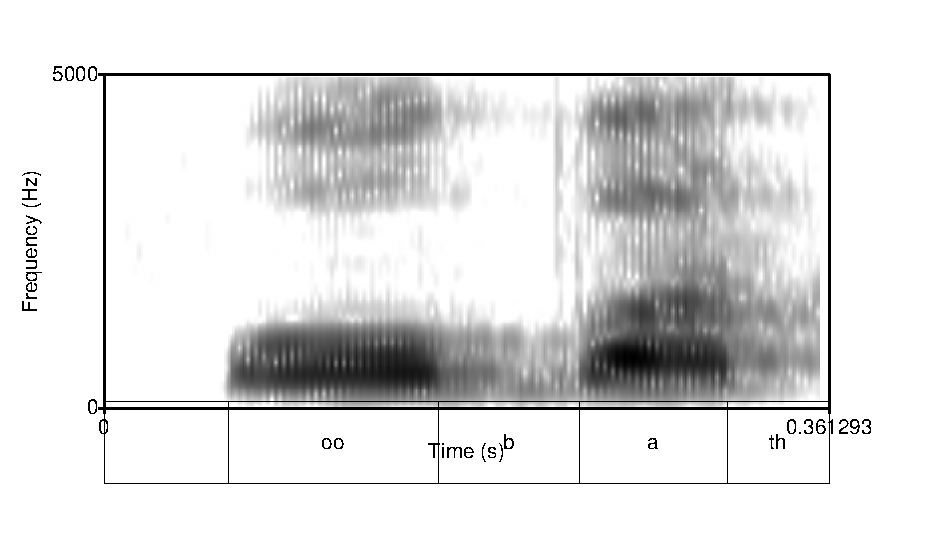
\includegraphics{pics/oobath.eps}
	\caption[Absence of a glottal stop before vocalic onset]{No glottal stop is found before the word initial [o:] in \phontrs{o:ba\dentt}{medicine}}
	\label{fig:phon:oobath}
	%K051222nar04
\end{figure}

\citet{Tapovanaye1995} finds glottal stops  before initial vowels and after final vowels, but does not grant them phoneme status.
\citet{Bichsel} found a glottal stop before every initial vowel. For reasons of syllable structure, she granted phoneme status to it. She wanted to eliminate syllables without onset.  In my data, the glottal stop is clearly optional.  Figure \ref{fig:minthamEntha} shows a glottal stop. While it is tempting to treat this as a reflex of historical \phontrs{*m\E ntah}{raw} as opposed to historical \phontrs{*minta}{beg}, the occurrence of the glottal stop is too irregular between speakers and lexemes to establish a clear correlation pattern between historical /h\#/ and the occurrence of the glottal stop in the modern language.
There is variation as to whether the glottal stop occurs word-initially, \phonet{Pa:nak} or \phonet{a:nak} `child'. Word-medial but syllable-initial vowels do not get a glottal stop preposed (\phonet{\J a:u}`far', not *\phonet{\J a:Pu}). The differences between the data of the aforementioned authors and my data might be due to the fact that they worked with elicited lexemes, while the data this analysis is based on  naturalistic speech. In the context of an elicitation session (like the one which yielded the data for the spectrogram in Figure \ref{fig:minthamEntha}), a glottal stop is often inserted in citation forms of words before an initial vowel and after a final vowel. This glottal stop insertion is not very regular in non-citation contexts. \citet{Bichsel} and \citet{Tapovanaye1995} treat it as a regular process, but this is not supported by the data in my corpus.  Vowels in initial position are frequently found without glottal stop. As an example, the word \phontrs{o:ba\dentt}{medicine}, pronounced after a pause of about 0.7 seconds (not  represented completely in the graphic), does not receive a glottal stop, as can be seen from Figure \ref{fig:phon:oobath}.

In this description, I therefore do not assume a phonemic glottal stop. 

\subsubsection{Distinctions in place of articulation}\label{sec:phon:Distinctionsinplaceofarticulation}
This section provides minimal pairs for all possible pairs of two neighboring places of articulation.

\paragraph{Stops}
Distinctive places of articulation for stops are:  labial, dental, apical, palatal, and velar. Apical comprises postalveolar and retroflex allophones. Apical as it is used in this description never comprises dental stops. In phonemic representation, /t/ will be used for apical stops, while the allophones will be represented as \phonet{\postalvt,\postalvd} and \phonet{\tz,\dz}.\\

\xbox{6}{
/p/ \textbf{vs.} /\dentt/
\ea
\gll  \textipa{ba:pa}  --- \textipa{ma:\dentt:a} \\
      father --- eye \\
\z      
}
\xbox{6}{
/b/ \textbf{vs.} /\dentd/
\ea
\gll  \textipa{ba\dentt a ba:\dentt a}  --- \textipa{\dentd a:\dentt ang} \\
      bricks --- come \\
\z      
}
\xbox{6}{
/\mb/ \textbf{vs.} /\ndentd/
 
n/a
     
}

\xbox{6}{
/\dentt/ \textbf{vs.} /t/
\ea
\gll  \textipa{kO:\dentt OR}  --- \textipa{kO:\tz OR} \\
      dirt --- fool \\
\z      
}
\xbox{6}{
/\dentd/ \textbf{vs.} /d/
\ea
\gll  \textipa{\dentd u:a}  --- \textipa{\dz u:\V a} \\
      praise --- two \\
\z      
}
\xbox{6}{
/\ndentd/ \textbf{vs.} /\ndz/
 
n/a
 
}

\xbox{6}{
/t/ \textbf{vs.} /c/
\ea
\gll  \textipa{kO:\tz OR}  --- \textipa{cO:cO} \\
      fool --- kind.of.fruit \\
\z      
}
\xbox{6}{
/d/ \textbf{vs.} /\J/
\ea
\gll  \textipa{a:\dz a}  --- \textipa{a:\J aR} \\
      exist --- teach \\
\z      
}
\xbox{6}{
/\ndz/ \textbf{vs.} /\nJ/
\ea
\gll  \textipa{\dentt a:\ndz ak} --- \textipa{pa:\nJ aN} \\
      dance --- long \\
\z
}

\xbox{6}{
/c/ \textbf{vs.} /k/
\ea
\gll  \textipa{cu:ci}  --- \textipa{ku:ciN} \\
      wash --- cat \\
\z      
}
\xbox{6}{
/\J/ \textbf{vs.} /g/
\ea
\gll  \textipa{\J a:ga}  --- \textipa{ga:\J a} \\
      protect --- elephant \\
\z      
}
\xbox{6}{
/\nJ/ \textbf{vs.} /\nG/
\ea
\gll   \textipa{pa:\nJ aN}   --- \textipa{ma:\nG a} \\
      long --- mango \\
\z
}





\paragraph{Fricatives}
There are only two native fricatives, /s/ and /h/, for which example \xref{ex:phon:min:sh} provides a near minimal pair. In Tamil \phonet{s} and \phonet{c} are allophones of /c/ ({\btam \TAMc \etam}) \citep[174]{Suseendirarajah1973phon}.
 Therefore it is necessary to establish that these phonemes are indeed different in SLM. Examples \xref{ex:phon:min:stsh} shows this. For the sake of completeness, example  \xref{ex:phon:min:sdzh} proves that /s/ is  also different from /\J/. /\sh/ and /z/ are only found in loanwords.\\

\xbox{5}{
/s/ \textbf{vs.} /h/
\ea\label{ex:phon:min:sh}
\gll  \textipa{kO:sON}  --- \textipa{pOhON} \\
     empty --- tree \\
\z      
}
\xbox{5}{
/s/ \textbf{vs.} /c/
\ea\label{ex:phon:min:stsh}
\gll  \textipa{ba:sa}  --- \textipa{ba:ca} \\
      wet --- read \\
\z      
}
\xbox{5}{
/s/ \textbf{vs.} /\J/
\ea\label{ex:phon:min:sdzh}
\gll  \textipa{ba:sa}  --- \textipa{bla:\J aR} \\
       wet --- learn \\
\z      
}

/f/ is marginally phonemic and is found in a few words or Arabic origin, like \phontrs{fi\dentt ena}{slander} and \phontrs{kafan}{shroud}, besides proper names and religious terms.


\paragraph{Nasals} The following list provides minimal pairs for all pairs of neighbouring nasals. Note that there is no dental nasal phoneme,\footnote{\phonet{\textsubbridge{n}} does occur before dental stops, but this is always the result of assimilation.} hence /m/ and /n/ are neighbours.\\

\xbox{14}{
/m/ \textbf{vs.} /n/ \textbf{vs.} /\ny/ \textbf{vs.} /\ng/
\ea
\gll  \textipa{\dentt a:ma}  --- \textipa{\dentt a:na} --- \textipa{\dentt a:\ny a}  --- \textipa{\dentt a:NaN}\\
      before --- soil ---  ask --- hand                                 \\
\z      
}\\
% \xbox{5}{
% /n/ \textbf{vs.} /\ny/
% \ea
% \gll  \textipa{O:nE\dentt}  --- \textipa{m^wO\ny E\dentt} \\
%       creeper --- monkey \\
% \z
% }
 
\paragraph{Glides}
SLM has two glides, /\V/ and /j/. These are distinctive as the following examples show.\\

\xbox{7}{
/\V/ \textbf{vs.} /j/
\ea\label{ex:phon:min:w}
\gll sa:\V a --- sa:ja\ng \\
      fields  --- love  \\
\z      
}

\paragraph{Phonemic status of the glides}\label{sec:phon:nonphonemicglideformation}
Some occurrences of the glides, like those in \xref{ex:phon:min:w}, are clearly phonemic and present in the underlying form. Other occurrences could be the result of a phonological constraint banning hiatus, especially when a long vowel is involved. This is schematized in \xref{ex:phon:glide:threemorae} \citep[cf.][23]{Tapovanaye1995}.

\ea\label{ex:phon:glide:threemorae} CV$_i$.V$_j\to$CV$_i$\textipa{:}V$_j\to$CV$_i$GV$_j$\z

or, in a more formal way

\ea\label{ex:phon:glide:threemorae:formal} $[+vocalic][+vocalic]\to[+vocalic][-vocalic]/\_[+vocalic]$ \z

The second vowel in a two-vowel sequence is not realized as vocalic in front of a third vowel. Evidence for this comes from the absence of a long vowel in environments which would normally require one (Section \ref{sec:phon:Vowellength}, p. \pageref{sec:phon:Vowellength}). An example is \phontrs{lija\dentt}{see}, where we would normally expect \phonet{li:a\dentt} or \phonet{li:ja\dentt} with a long vowel. This problem of the missing long vowel can be solved if we assume that the sequence VG is a special realization of a long vowel.
It would then appear that the second part of the vowel is turned into a glide, leaving only the first part as vocalic and thus resulting in a short vowel.
Next to /i/, this is found for /u/, for example in \phontrs{bu\V aN}{throw}, where the right part of the long /u/ is turned into a glide.
% Some evidence for this can be found in a transcript made by a native speaker (K051205nar05), who wrote the word for `to get up' once with a long vowel (\em baaung\em), and once with a short vowel followed by a glide (\em bavung\em).

If the first vowel is neither /i/ nor /u/, the glide formation is not found, resulting in hiatus as in \phontrs{\J a:u}{far}.\footnote{The phonological conditions of a preceding high vowel in order to form a glide are actually a common feature of Austronesian languages \citep[116]{Himmelmann2005typochar}.} In these cases, a long vowel is always found. Also note that a short vowel in the penultimate syllable of  disyllabic words is only possible if the onset of the final syllable is a glide. This distribution strongly suggests that [ij] and [u\V] are alternative realizations of a lengthened /i/ and a lengthened /u/.

The analysis of the creation of a sequence VG out of a long vowel is complicated by the fact that there are some words with a sequence V\textipa{:}G, like those given in \xref{ex:phon:min:w}. While in \xref{ex:phon:min:w}, this is not problematic because /a/ does not have a corresponding glide, there are also some words where a long [+high] vowel is followed by a glide, e.g. \phontrs{bu:\V a}{fruit}. This can be analyzed as an underlying form /bu.\V a/, which undergoes the regular vowel lengthening process of open penultimate syllables in disyllabic words. There are thus words of the type /CV.V(C)/ like \phonem{bu.aN} which have to be distinguished from words of the type /CV.GV(C)/ like \phonem{bu.\V a}.\footnote{For an  argument for the theoretical distinction between phonemic and non-phonemic glides see \citet{Levi2008glides}.}

The only other instance where a short vowel is found in the open penultimate of a disyllabic lexical word is in the sequence V$_i$hV$_i$ (e.g. \phontrs{leheR}{neck}). There might be the possibility to explain this sequence in a manner akin to the occurrence of non-phonemic glides, similar to the solution proposed by Tapovanaye (see Section  \ref{sec:phon:Problematiccases}), but this needs more theoretical research.


 
% /\dentd unia/ `world' is normally pronounced \phonet{\dentd unija}. The non-phonemic character of the glide in this word can be seen by the lack of length in the /i/.





\subsubsection{Manner and voicing distinctions}\label{sec:phon:Mannerandvoicingdistinctions}
Having discussed the different places of articulation, we now discuss the different manners of articulation available for the different places of articulation. Voicing contrasts are also discussed here for convenience.

\paragraph{Distinctions for labial consonants}
{~}\\

\xbox{14}{
/p/ \textbf{vs.} /b/ \textbf{vs.} /m/ \textbf{vs.} /\V/
\ea
\gll  \textipa{sa:pa}  --- \textipa{Ra:ba} --- \textipa{sa:ma} --- sa:\V a\\
       who? --- caress  --- together --- fields\\
\z      
}\\ 

\paragraph{Distinctions for coronal consonants}

{~}\\
\xbox{14}{
/\dentt/   \textbf{vs.} /s/ \textbf{vs.} /n/ \textbf{vs.} /r/ \textbf{vs.} /l/
\ea
\gll  \textipa{ga:\dentt al}    --- \textipa{Ra:sa} 	--- \dentt a:na --- \dz a:\textipa{R}a --- sa:la \\
      itch 			---  tasty 		--- soil --- blood --- wrong\\
\z      
}\\

\xbox{14}{
/\dentt/ \textbf{vs.} /t/ \textbf{vs.} /d/  \textbf{vs.} /s/ \textbf{vs.} /n/ \textbf{vs.} /r/ \textbf{vs.} /l/
\ea
\gll   \textipa{ku:\dentt u} --- \textipa{lu:\tz u\dentt}  --- \textipa{\dz u:\dz uk} --- su:su --- gu:nu\ng{} --- \textipa{\dentt u:RuN} --- \textipa{spu:lu} \\
      louse --  knee --- sit --- milk --- mountain --- get.down --- ten \\
\z      
}\\


\xbox{14}{
/\dentd/ \textbf{vs.} /d/ \textbf{vs.} /\dentt/
\ea
\gll \textipa{\dentd u:a} --- \textipa{\dz u:\V a} --- \textipa{\dentt u:\V a}   ~~~~{\rm apical /t/ is not possible initial position} \\
      recital --- two --- old \\

\z
} \\


\xbox{14}{
/\dentt/ \textbf{vs.} /t/ \textbf{vs.} /d/
\ea
\gll \textipa{kO:\dentt OR} --- \textipa{kO:\tz OR} --- \textipa{kO:\dz Ok}   \\
      dirt --- fool --- frog \\
\z
} \\


\xbox{14}{
/\dentd/ \textbf{vs.}  /d/
\ea
\gll pa\dentd eRi --- a:\postalvd e \\
     struggling --- younger.sibling  \\
\z
} \\


\xbox{14}{
\phonet{\textsubplus{\:r}} (allophone of /d/) \textbf{vs.} \phonet{R} (allophone of /r/)
\ea
\gll \rm{\textipa{\dz a:\textsubplus{\:r}a}} --- \rm{\textipa{\dz a:Ra}}\\
       chest --- blood\\
\z      
}\\



\paragraph{Distinctions for palatal consonants}
{~}\\

\xbox{7}{
/c/ \textbf{vs.} /\J/ \textbf{vs.} /\ny/
\ea
\gll  \textipa{ca:Ri}  --- \textipa{\J a:\postalvd i} --- \textipa{\ny a:\ny i} \\
       find --- become --- sing\\
\z      
}\\ 

\paragraph{Distinctions for velar consonants}
{~}\\

\xbox{7}{
/k/ \textbf{vs.} /g/ \textbf{vs.} /\ng/
\ea
\gll  \textipa{kla:ki}  --- \textipa{\dz a:giN} --- \textipa{a:NiN}  \\
       boy --- beef --- air \\
\z      
}\\ 




\subsubsection{The prenasalized stops}\label{sec:phon:Theprenasalizedstops}

\begin{figure}
 \centering 
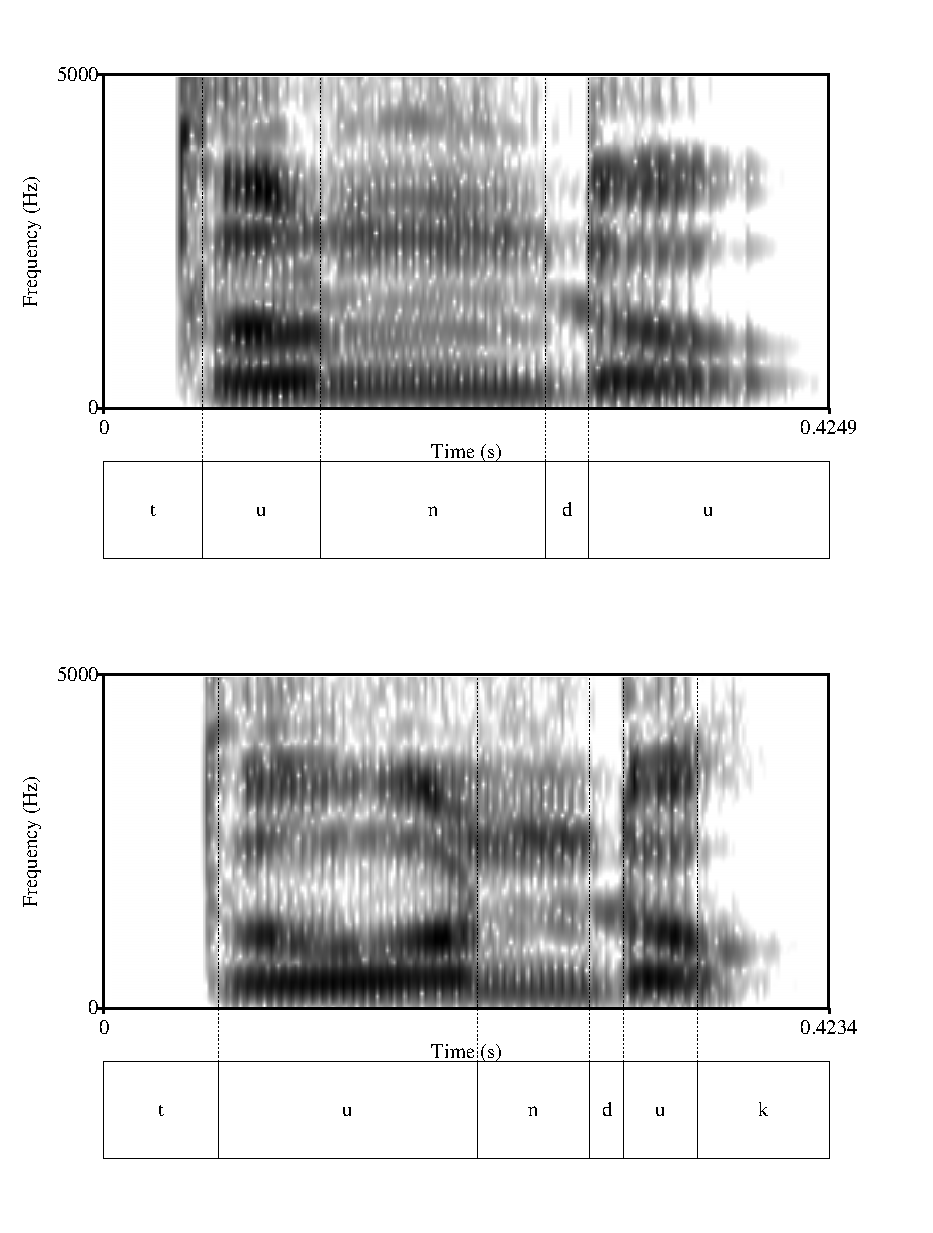
\includegraphics[width=.8\textwidth]{pics/thunduthuunduk.eps}
%  Spectrogram-non-prenasalized-consonant.png: 432x252 pixel, 72dpi, 15.24x8.89 cm, bb=0 0 432 252
\caption[Spectrogram of tautosyllabic and heterosyllabic NC-clusters]{The heterosyllabic sequence /n.d/ in the Tamil loan \phontrs{\dentt u\nz.\dz u}{piece} has a short vowel (69ms) and a comparably longer nasal (132ms) than the tautosyllabic sequence /.nd/ in the native word \phontrs{\dentt u:.\ndz uk}{bend} below (151ms+66ms). The latter sequence is analyzed as a phonemic prenasalized consonant in this grammar.}
\label{fig:thunduthuunduk}
\end{figure}

SLM has four prenasalized stops matching the points of articulation of the non-prenasalized stops. The dental prenasalized stop is not found. Prenasalized stops contrast with N+stop clusters both phonetically and phonologically. Phonetically, the prenasalized consonants have a much shorter nasal phase (Figure \ref{fig:thunduthuunduk}). Phonologically, vowels preceding prenasalized consonants are lengthened when in penultimate position of disyllabic stems (for more discussion of vowel lengthening see Section \ref{sec:phon:struct:Roots}). This suggests that the prenasalized consonants do not close the preceding syllable. N+stop clusters, on the other hand, never occur after a long vowel, suggesting that the nasal part closes the preceding syllable. This absence of vowel lengthening in heterosyllabic clusters can also be seen  in Figure \ref{fig:thunduthuunduk}, where the vowel is shorter before the N+C cluster of \phontrs{\dentt u\nz\dz u}{piece} (above), and longer before the prenasalized \nd{} in \phontrs{\dentt u:\ndz uk}{bend} below.

Both heterosyllabic and tautosyllabic NC sequences are listed in 
 Table \ref{tab:PrenasalizedConsonants}, together with some other combinations of voiced stop and/or nasal.
\begin{table}
	\begin{center}
	% use packages: array
	\begin{tabular}{ccccccc}
	 		& V\textipa{:}.CV 			& VC.CV 			& V\textipa{:}.NV 				& VN.NV   			& VN.CV					& V\textipa{:}.\super{N}CV \\
	\hline
	labial   	& \tbltrs{ba:i}{pig}		& \tbltrs{hab:aR}{news}		& \tbltrs{\dentt a:ma}{earlier}	& \tbltrs{sam:a}{every}	  	&  \parbox{2.5cm}{\centering\textipa{sambal} \\`{spicy food}'}	& \tbltrs{ga:\mb aR}{picture}\\\\
	dental   	& n/a			& n/a				& 	n/a				&  	n/a			& \tbltrs{seli\dentn\dentd i}{spider} 	& n/a 				\\\\
	apical		& \tbltrs{li:\dz a}{tongue}	& \tbltrs{pI\dz:ang}{sword}	& \tbltrs{pi:nang}{areca nut}		&  \tbltrs{bIn:ang}{thread}	& \tbltrs{\dentt u\nz\dz u}{piece} 	& \tbltrs{\dentt u:\ndz uk}{bent}  \\\\
	palatal  	& \tbltrs{ga:{\J}i}{salary}	& \tbltrs{ha\J:i}{Haj}	& \tbltrs{\ny a:\ny i}{sing}	& \tbltrs{ba\ny:ak}{much}		& \tbltrs{a\ny\J iN}{dog}		& \tbltrs{ba:\nJ iR}{flood}\\\\
	velar    	& \tbltrs{\dentt i:{g}a}{three}	& \tbltrs{sIg:aR}{healthy}	& \tbltrs{i:Na\dentt}{think} 		&  \tbltrs{\dentt IN:a}{middle}& \tbltrs{siNga}{lion}			& \tbltrs{mni:\nG al}{die} \\\\
	\hline\hline
	\end{tabular}
	\caption[Medial combinations of nasal and stop]{Prenasalized consonants in opposition to plain and geminated stops, plain and geminated nasals, and clusters of nasal+stop. Dental stops normal do not occur word-medially. \phontrs{seli\dentn\dentd i}{spider} is an exception, a loanword from Tamil.}
	\label{tab:PrenasalizedConsonants}
	\end{center}
% pa\dentn\dentd el ceremony.cloth
% tIndang kick
% piiNDa spread
\end{table}


% 
% Prenasalized stops have been proposed by \citep{Thera1986, Tapovanaye1995}. \citet{Bichsel} argues against prenasalized stops because they would increase the phoneme inventory. Other authors have remained by and large silent on this subject, but \citet{SmithEtAl2004} regard Bichsel's analysis as superior.
% Tapovanaye's analysis is based on the observation that long vowels can generally only occur in open syllables. The only exception to this are syllables closed by a nasal homorganic to the following stop, i.e. V:mbV, V:n\dentd V, V:nd V, V:\ng gV. In order to retain his rule of vowel lengthening in open syllables, Tapovanaye analyzes these sequences as V:.\mb V, V:.\ndentd V, V:.\ndz V, V:.\nG V, shifting the nasal to the onset of the following syllable. Bichsel misreads the proposal as suggesting that \mb{} and b, \ndentd{} and \dentd{} etc. would be allophones and shows convincingly that they are not, but Tapovanaye had never claimed that. Some parts of Bichsel's comments refer to the analysis which Tapovanaye intended and object that such an analysis would increase the size of the phoneme inventory by four, namely \mb, \ndentd, \ndz{} and \nG\footnote{Bichsel does not list /\ndzh/ as a phoneme, otherwise the increase would have been by five.}. This is of course true, but a phoneme inventory should contain all sounds which matter on the phonological level of analysis, and there is no need to keep the size of an inventory smaller than necessary. On phonological grounds alone, there is enough reason to accept the prenasalized stops as members of the phoneme inventory, because they allow for a straightforward explanation of vowel lengthening in open syllables, a generalization that cannot be captured otherwise. But instrumental analysis also shows that the sequences NC and \u{N}C differ phonetically. Figure \xref{fig:phon:sambalgaambar} shows  spectrograms of the word \phontrs{sambal}{sauce} and \phontrs{ga:\mb aR}{picture}. The  nasal in \em ga:\mb ar \em is clearly shorter than the nasal in \em sambal \em.

Additional support for the phonemic status of the prenasalized consonants comes from acceptability judgments. Speakers were asked whether \em sambal \em and \em ga:\mb ar \em could be written with the sequence \graphem{m+b} ({\SHa\char253}{\SHa\-\char237a}) or the prenasalized consonant \graphem{\mb} ({\SHb\char117a}) in Sinhala script. Informants generally accepted the writing \graphem{m+b} for both forms, but the writing \graphem{\mb} only for \em ga:\mb ar\em. Analogous results were obtained for words with other prenasalized consonants. This shows that these sounds are cognitively different for the speakers, otherwise they should have been treated alike. This is even more significant given that the vowel preceding a prenasalized stop tends to be reduced in Sinhala, but lengthened in SLM. Artefacts in the choice of grapheme resulting from vowel quality can therefore be excluded.

\subsubsection{The palatal obstruents}\label{sec:phon:Thepalatalobstruents}  
SLM numbers three palatal obstruents \phonem{c,\J,\nJ}, which, besides their realization as stops, have affricate allophones \phonet{\textcttctclig,\textctdctzlig,\super{\ny}\textctdctzlig}. Given that the other stops do not have the option of affrication, the question arises whether these phonemes pattern with the stops, or whether they are in a natural class of their own, the class of affricates (cf. \citet[63]{Bichsel}, \citet[357]{Noonan2006}). First, we have to establish whether they consist of one phoneme or two. In case they consist of only one phoneme, we have to answer the question whether this phoneme is internally complex.

\citet{Trubetzkoy1939} contains a list of rules how to decide between the `monophonematic' and the `polyphonematic' analysis of a certain part of the sound sequence (\em Schallstrom\em). Particularly relevant for SLM are the rules IV and VI, which are given below.

\begin{quote}
Regel IV. Eine potentiell monophonematische \el{} Lautverbindung muß als Realisation eines einzigen Phonems gewertet wetden, wenn sie als Einzelphonem behandelt wird, d.h. wenn sie in solchen Lautstellungen vorkommt, wo in der betreffenden Sprache Phonemverbindungen nicht zugelassen werden.\footnote{A potentially monophonematic sound combination must be seen as the realization of exactly one phoneme if it is treated as a single phoneme, i.e. if it occurs in environments where the language under discussion does not admit combinations of phonemes.}
 \citep[53]{Trubetzkoy1939}
\end{quote}

\begin{quote}
Regel VI. Wenn ein Bestandteil einer potentiell monophonematischen Lautverbindung nicht als kombinatorische Variante irgendeines Phonems derselben Sprache gedeutet werden kann, so muß die ganze Lautverbindung als Realisation eines Eigenphonems gewertet werden.\footnote{If a part of a potentially monophonematic sound sequence cannot be analyzed as a combinatorial variant of any phoneme of the same language, then the whole sound sequence must be seen as a realization of one phoneme.}
\citep[54]{Trubetzkoy1939}
\end{quote}

Rule IV states that a sequence must be analyzed as one phoneme if it occurs in a context where the language demands that only one phoneme be present, not more. In SLM, complex onsets are such a context. A complex onset can be formed by one consonant followed by any of /r,l,\V,j/ (see \ref{sec:phon:Syllablestructure} for more discussion). This can be schematized as CXV, where X is one of the phonemes just listed. The word \phontrs{cRi:\dentt a}{story} has an /r/ in the second position. Preceding the /r/, only one phoneme is permitted by SLM syllable structure. Therefore, the sound sequence preceding /r/ must be analyzed as one phoneme /c/, not as a sequence of several phonemes, like /\textctt\textctc/. The argumentation for words like \phontrs{\J le:na}{window} is analogous.

Rule VI states that a sound sequence should not be analyzed as consisting of several phonemes if this would lead to the postulation of phonemes otherwise not found in the language. If the palatal obstruents are   analyzed as polyphonematic, consisting of a stop and a following fricative, this yields to the postulation of palatal fricatives. Palatal fricatives are not found elsewhere in SLM phonology. Therefore, the palatal obstruents must be analyzed as monophonematic.

We now have  firm evidence that the palatal obstruents are monophonematic. The following question is whether we have to assume a complex internal structure within the phoneme. In German, for instance, \trs{Tal}{valley} and \trs{[\texttslig]ahl}{number} are distinguished by the former word having a simple monophonematic onset, while the latter has a complex monophonematic onset. There other features like voicing and place of articulation being alike, we need to recur to the internal structure of the phoneme to capture the difference between /t/ and /\texttslig/. In SLM, such distinctions are not necessary. The palatal obstruents \phonem{c,\J,\nJ} are not in opposition to other segments which would require the distinction between simple and complex internal structure.

The last question is whether the palatal obstruents form a natural class with the other stops, or whether they are in a class of their own. The palatal obstruents behave in most ways like the other stops, and can occur in all places the stops can occur, affording the same phonological generalizations like vowel lengthening (Section \ref{sec:phon:Vowellength}) or gemination after schwa (Section \ref{sec:phon:Consonantlength}). One exception to this rule is word-final position, where palatal obstruents are never found. This, however, need not be a result of \phonem{c,\J,\nJ} being distinct from the other stops, it rather seems to be a constraint banning palatals from this position since \ny{} is also disallowed there.\footnote{The palatal glide \phonet{j} does occur in some words in final position, but this is uncommon.}\footnote{Standard Malay and Jakartanese also have a constraint against palatals in final position \citep[12,32]{Adelaar1985}.}

To conclude, the palatal obstruents can safely be treated as stops, there is no need them any different from other stops in phonology, but their phonetic realization can contain a fricative phase.\footnote{See \citet{Clements1999affr} and \citet{Kehrein2002affr} for more theoretical discussion of phonetic affrication of palatal stops.}

\subsubsection{Major consonantal allophones}\label{sec:phon:Majorconsonantalallophones}
This section discusses the free and complementary  allophones of consonantal phonemes.

\paragraph{Stops}
/p, \dentt, t, c, k/  are unaspirated voiceless stops. /b, \dentd, d, \J, g/ are voiced stops. SLM voiceless consonants have a VOT close to zero (0-10ms), voiced consonants have a negative VOT and tend to be fully voiced.\footnote{
Voice onset time (VOT) is a measure used for consonants. It indicates the relative timing between the release of the articulatory stricture and the beginning of voicing, i.e. the vibration of the vocal chords \citep[19f]{Ladefoged1975course}. A  positive VOT is indicative of aspiration, unaspirated voiceless consonants have a VOT around 0, while a negative VOT is indicative of voiced consonants.}
The appendix (p. \pageref{sec:VOT}) contains spectrograms illustrating this for a number of environments, namely the onset, intervocalic position, and following /s-/.


Phonologically apical /t, d/ are realized as retroflex [\tz,\dz] before /a,o,u/  and as postalveolar [\postalvt, \postalvd] before /e,i/.

The voiced apical stop /d/ can be realized between a vowel and /a,o,u/ as either a voiced retroflex stop \phonet{\dz} or a  postalveolar tap \phonet{\textsubplus{\:r}}.\footnote{See \citet[14]{Schiffman1999} for a similar process in Spoken Indian Tamil.} This seems to depend on speech tempo but also on the individual lexeme. In the frequent lexeme /pada/, `\textsc{plural}', this is almost always the case, whereas the lexeme /duduk/ `sit,stay,be', which is about as frequent as /pada/, the tap is found less often. \phonet{\textsubplus{\:r}} as a  realization of /d/ must not be confounded with \phonet{R} as a realization of /r/. The minimal pair \phonet{\dz a:\textsubplus{\:r}a} `chest' and \phonet{\dz a:Ra} `blood' attests to this.

The palatal stops are    realized as stops [c, \J{}] or as affricates [\textcttctclig,\textctdctzlig]. Affrication seems to be more common for the voiceless palatal stop

/p, b, \dentt, \dentd, g, k/ and the prenasalized stops have no noteworthy allophones.

All mentioned stops with the exception of /\dentd/ occur simple or as geminates, but geminate /t/ only occurs in loanwords from Tamil, such as \phontrs{ka\postalvt:il}{bed}.
 

% The velar stops are very fronted in some of my consultants' speech and could even be called palatal. This does not only occur before front vowels (\phonet{\textbardotlessj ihila},`mad') but also before other vowels (\phonet{\textbardotlessj O:l}`Galle (town)').

\paragraph{Fricatives}
/s/ is realized as [s] and,  rarely, /s/ can be realized as [h], as in the following examples, where the normal pronunciation would be \phonet{sam:a} (cf. \citet[65]{Bichsel}, \citet{SmithEtAl2004}).

\xbox{14}{
\ea  
\gll  kaRaN in:i     \textbf{h}am:a s-abis\\
      now \textsc{prox} all \textsc{past}-finish  \\
    `Now all was finished'  (K060116nar11)
\z      
}\\ 

\xbox{14}{
\ea 
\gll si:ni kla:ki pRompa\ng{} \textbf{h}am:a a\dentn\dentt i-\dentt a:\ndz ak \\
     here boy girl all \textsc{irr}=dance  \\
    `Here, boys and girls will all dance (together).' (K060116nar10)
\z
} \\

The alternation between /s/ and /h/ is also found in colloquial Sinhala \citep[18]{Matzel1983}, where it is completely generalized. In SLM, it is a very marginal phenomenon \citep[cf.][65]{Bichsel}.
 
/h/ is a rare phoneme. While other varieties of Malay make more use of /h/, historically present initial h- has been lost in many words in SLM everyday speech \citep[ch.4.3]{Paauw2004}. It is sometimes pronounced in a handful of words for reasons of prestige, \phontrs{(h)a:Ri}{day}{} being by far the most frequent one. Words which retain initial /h/ are \phontrs{hab:aR}{news} and \phontrs{ha\dentt:u}{\textsc{indef}}, furthermore words of Arabic origin like \phontrs{ha\J:i}{Hajji} or \phontrs{halal}{permitted for Muslims}.

The distinction between /\textesh/ (occurring only in loanwords) and /s/ is frequently ignored.

\paragraph{Nasals}
/m/ is  labialized before long \phonet{o:}, as in \phonet{m\super wo:\ny E\dentt} `monkey'.


Within a morpheme, nasals are not distinctive in preconsonantal position. Their place of articulation is always homorganic to the following consonant (\phonet{mp, \dentn\dentt, \nz\dz, \ny c, \ng k, mb} etc.). Coincidentally, this is the only way to produce a dental nasal.  Between morpheme boundaries, non-homorganic nasals can be found, e.g. \phontrs{o:Ra\ng pa\dz a}{man \textsc{pl}}, where a velar nasal meets a labial stop. But even in this position, assimilation is often found (/ora\ng{} pada/$\to$\phonet{o:Rampa\dz a}).

Word-finally,  nasals are often rendered as velar (\phontrs{se:lon\~{}se:loN}{Ceylon}), but this is not obligatory (\citet{Bichsel,Saldin2001,SmithEtAl2004}, \em contra \em \citet{Adelaar1991}). The following words illustrate that the place of articulation is distinctive in word-final position:


\xbox{14}{
\ea 
\gll a:Ram --- makanan --- ba:Ra\ng \\
     charcoal --- food --- goods  \\
\z
} \\

The former two could be heard with a velar nasal, but do also occur with the indicated consonant, whereas the final word can never occur with any other nasal than the velar one. This shows that speakers can neutralize the distinction in word final position, but this is facultative.


\paragraph{Liquids}
Consonant length (see next section) entails a difference in manner of articulation for /r/. Short /r/ is an alveolar tap \phonet{R}; long /r/ is an alveolar trill \phonet{r} (see Figure \ref{fig:kiiringkirring}).

/l/ has no noteworthy allophones.

\begin{figure}
 \centering
 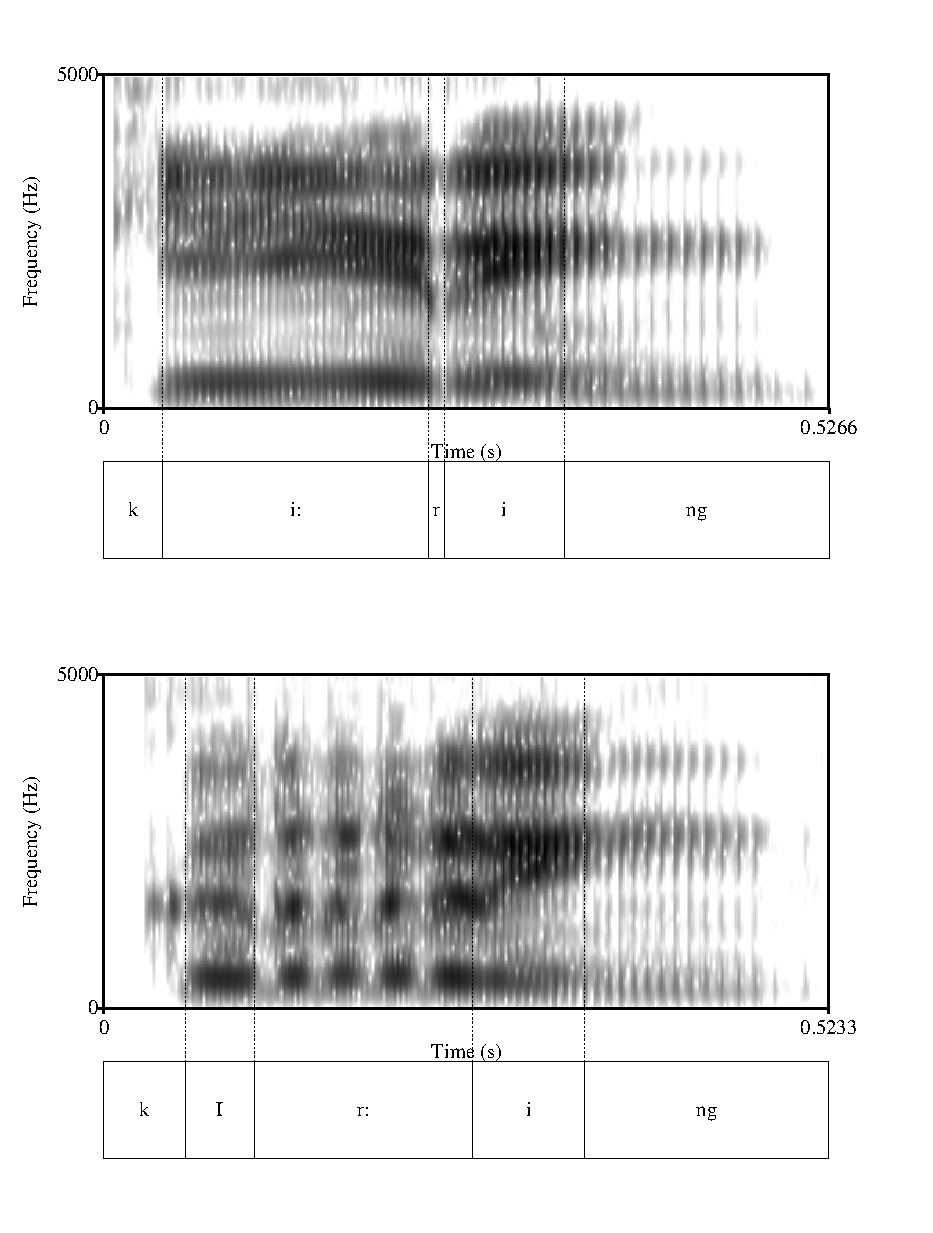
\includegraphics[width=.8\textwidth]{pics/kiiringkirring.eps}
 % pErrang-spectro.png: 432x252 pixel, 72dpi, 15.24x8.89 cm, bb=0 0 432 252
 \caption[Differences in length and vowel quality between \phontrs{ki:RiN}{send}   and \phontrs{kIr:iN}{dry}]{The words \phontrs{ki:RiN}{send} (above) and \phontrs{kIr:iN}{dry} (below) show a number of things. First, the formant structure of the first vowel is different, showing that [i] as a realization of /i/ must be distinguished from \phonet{I} as a realization of /\E/. Second, they show the complementary distribution of long vowels and long consonants. The word above has a long vowel (206ms) and a short consonant (11ms), while the word below has a short vowel (50ms) and a long consonant (158ms). The spectrograms furthermore show that short /r/ is realized as a tap with minimal duration, while phonemically long/geminated r is realized as a trill. }
 \label{fig:kiiringkirring}
\end{figure}

\subsubsection{Consonant length}\label{sec:phon:Consonantlength}

All consonants besides the prenasalized stops, \dentd{} and \V{} can occur lengthened in intervocalic position. Long vowels and long consonants are mutually exclusive. \xref{ex:phon:longcons:thiikam} shows a near minimal pair with a) a long vowel and a short consonant and b) a short vowel and a long consonant (see also Figure \ref{fig:soopithoppi}).

\xbox{14}{
\ea \label{ex:phon:longcons:thiikam}
\ea
\gll  so:pi \rm CV\textipa{:}CV \\
      liquor   \\
\ex
\gll \dentt op:i \rm CVC\textipa{:}V\\
hat\\
\z
\z
} \\

\begin{figure}
 \centering
 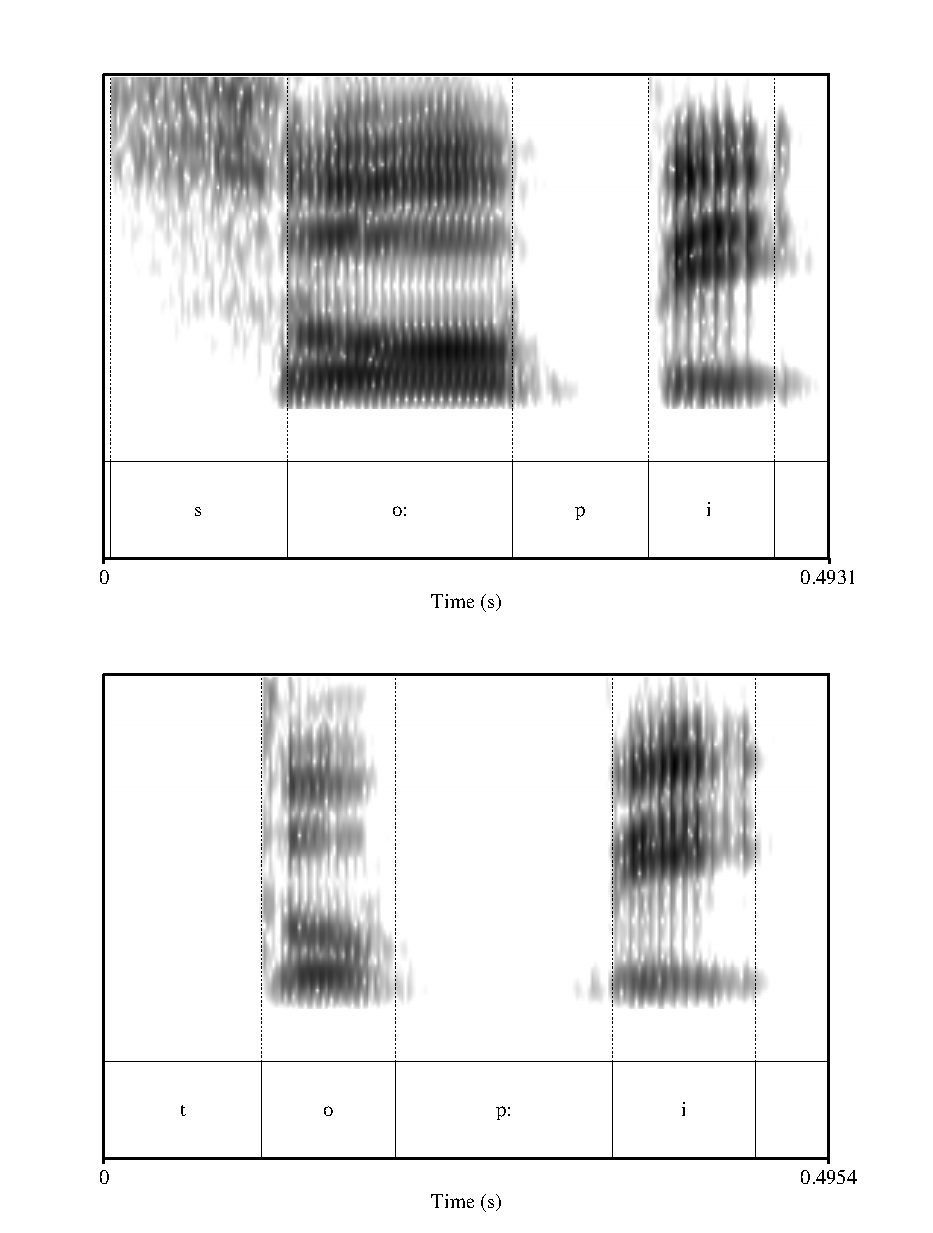
\includegraphics{pics/soopithoppi.eps}
 % soopithoppi.eps: 1179668x1179666 pixel, 0dpi, infxinf cm, bb=
 \caption[Vowel and consonant length in \phontrs{so:pi}{liquor} and \phontrs{\dentt op:i}{hat}]{The word \phontrs{so:pi}{liquor} has a long vowel (153ms) and a short consonant (93ms), while the word \phontrs{\dentt op:i}{hat} has a short vowel (91ms) and a long consonant (149ms).}
 \label{fig:soopithoppi}
\end{figure}





Two types of long consonants can be distinguished on phonological grounds: Underlyingly long consonants, as in \phontrs{\dentt op:i}{hat}{} or \phontrs{ik:a\ng}{fish}, and lengthened consonants such as in \phontrs{s\I g:aR}{healthy}. The former  always have a long consonant,\footnote{In certain types of compound, like \phontrs{kap:al+\dentt IRbaN=kapal\dentt IRbaN}{ship+fly=plane}
the long consonant optionally disappears. These are rare.} while the latter only have a long consonant if the consonant is located between penultimate and final syllable. If, through affixation, the consonant is found at another position, it is not geminated. Lengthened consonants can only occur after schwa, while underlyingly long consonants can occur after /a/ \phontrs{a\dentt:as}{top}, /e/ \phontrs{pe\dentt:a}{parrot}, /i/ \phontrs{ik:a\ng}{fish}{} and  /o/ \phontrs{\dentt op:i}{hat}. No long consonant has been found after /u/ or schwa.
Tables \ref{tab:PositionsAndGeminationsOfConsonants:stops} and \ref{tab:PositionsAndGeminationsOfConsonants:other}  contain a column of words with long consonants.

There is only one instance of a long palatal glide, \phontrs{maj:e\dentt}{corpse}.

Phonetically, long consonants are of about 1.5 times the duration of shorter consonants, as can be seen from Figure \ref{fig:soopithoppi}.

% \begin{figure}
%  \centering
%  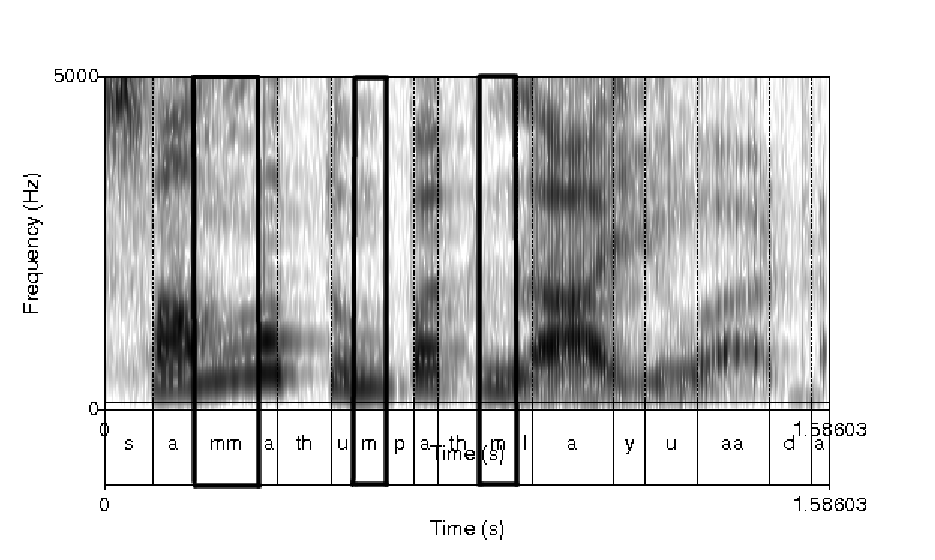
\includegraphics[height=0.3\textheight]{./pics/sammathumpathmlaayuaada.eps}
%  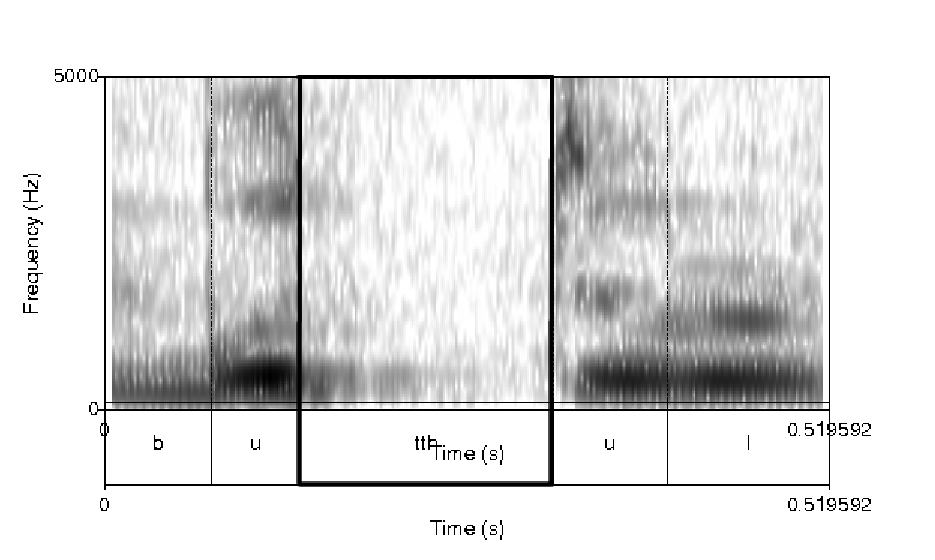
\includegraphics[height=0.3\textheight]{./pics/butthul-length.eps}
%  \caption{The first occurrence of [m] in the spectrogram above is a long consonant. Its duration is 0.144s. The further occurrences are short, the second one lasts 0.072s, the third one, 0.083s. Below, we see a long dental stop in the word \phontrs{bu\dentt:ul}{very}.}
%  \label{fig:phon:conslength:sammathumpathmlaayuaada}
% \end{figure}
% 
% \begin{figure}
%  \centering
%  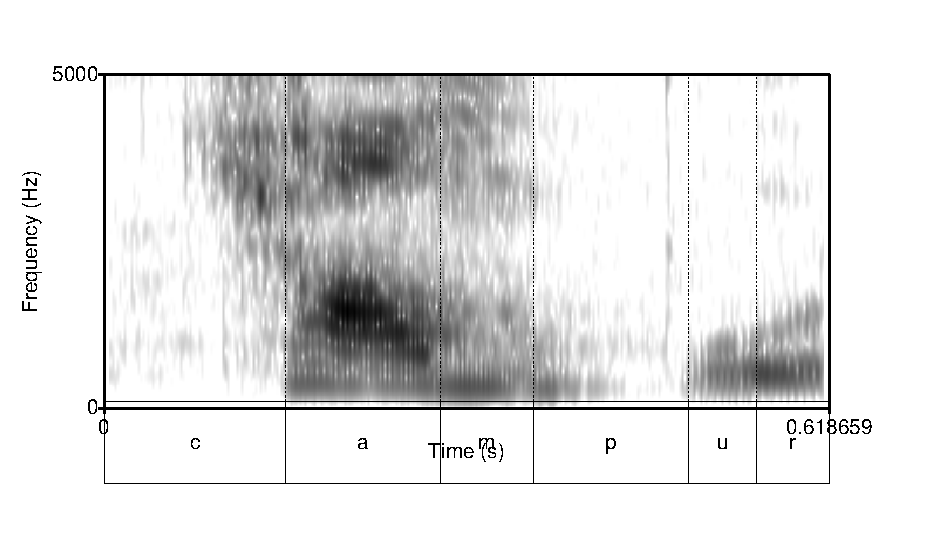
\includegraphics[height=0.3\textheight]{./pics/campur.eps}
%  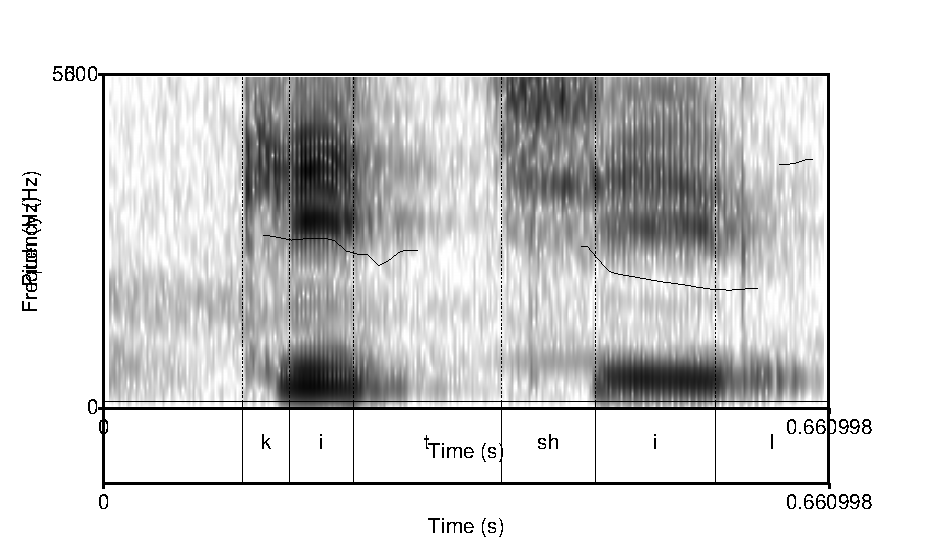
\includegraphics[height=0.3\textheight]{./pics/kiccil.eps}
% \caption{When long palatal stops are pronounced as affricates, the occlusion part last slightly longer than the fricative part. Above, we see a short palatal in the onset, while below in the word \phontrs{kic:il}{small}, the occlusion part has a duration of 0.131ms, and the fricative part has a duration of 0.082s.}
%  \label{fig:phon:conslength:kiccil}
% \end{figure}


\subsubsection{Distribution of consonants}\label{sec:phon:Distributionofconsonants}
All consonants may occur in intervocalic position, but \dentd{} is very rare there, one instance is \phontrs{kO\dentd aRa\dentt}{miracle}.
All consonants but \ng{} and the prenasalized stops may occur in  word-initial position, but the palatal glide is very rare there. There is only one word with initial \tz{}, \phonet{\tz ak:a\dentt a}, which emphasizes the rapid nature of an event and might very well be onomatopoetic, so that it would not have to obey the general phonological rules.

There are more constraints word-finally. Voiced stops, apical stops,  h, \ny{}\footnote{These four cannot occur word-finally in Sinhala, Tamil or Jakartanese either. -h\# can occur in Std. Malay, but the other three cannot.} and \V{}  cannot occur in final position in native words, although some of those are frequently found in English loan words (\em bag, pitch, bat\em).

Few consonants ever occur in the coda of syllables inside a morpheme. Those that do occur are the nasals, the liquids, /k/ and /s/ (see Tables \ref{tab:PositionsAndGeminationsOfConsonants:stops} and \ref{tab:PositionsAndGeminationsOfConsonants:other}). If roots combine with an affix or a clitic with an onset, like \phontrs{-king}{\textsc{caus}}{} or \phontrs{=pe}{\textsc{poss}}, any consonant which can occur morpheme-finally can occur in a word-medial coda.

Tables \ref{tab:PositionsAndGeminationsOfConsonants:stops} and \ref{tab:PositionsAndGeminationsOfConsonants:other} show examples for every consonant in initial and final position and also give  examples of the consonant in intervocalic position (short and long) and morpheme-internal coda position.


\begin{table}
	\begin{center}
		\begin{tabular}{llllll}
			& initial 			& intervocalic 	short		& intervocalic long & 	\parbox{2cm}{morpheme-internal coda}	 & final \\ % add column V_.CV
	\hline \vspace{0.2cm}
		p 	& \parbox[t]{2cm}{\textipa{pa:ke}\\`dress'}  & \parbox[t]{2cm}{\textipa{ba:pa}\\`father'}    & \parbox[t]{2cm}{\textipa{l\U p:as}\\`leave'} & \fbox{\parbox[t]{2cm}{~\\}} & \parbox[t]{2cm}{\textipa{g\I l:ap}\\`dark'} \\\vspace{0.2cm}
		\dentt  & \parbox[t]{2cm}{\textipa{\dentt a:na}\\`soil'}& \parbox[t]{2cm}{\textipa{u:\dentt an}\\`forest'}& \parbox[t]{2cm}{\textipa{a\dentt:as}\\`up'}      & \fbox{\parbox[t]{2cm}{~\\}} & \parbox[t]{2cm}{\textipa{bansa\dentt}\\`bedbug'} \\\vspace{0.2cm}
		t 	& \fbox{\parbox[t]{2cm}{~\\}}& \parbox[t]{2cm}{\textipa{ba:\tz ok}\\`coconut.shell'}&\fbox{\parbox[t]{2cm}{(\textipa{ka\postalvt:il})\\`bed'(Tam.)}} & \fbox{\parbox[t]{2cm}{~\\}} & \fbox{\parbox[t]{2cm}{~\\}}  \\\vspace{0.2cm}
		c	& \parbox[t]{2cm}{\textipa{campuR}\\`mix'}& \parbox[t]{2cm}{\textipa{ku:ci\ng}\\`cat'}    & \parbox[t]{2cm}{\textipa{kic:il}\\`small'}&\fbox{\parbox[t]{2cm}{~\\}}&\fbox{\parbox[t]{2cm}{~\\}}  \\\vspace{0.2cm}
		k 	& \parbox[t]{2cm}{\textipa{ka:ki}\\`leg'}    & \parbox[t]{2cm}{\textipa{ba:kaR}\\`burn'}     & \parbox[t]{2cm}{\textipa{ik:a\ng}\\`fish'} &\parbox[t]{2cm}{\textipa{\dentt aksiR}\\`think'}& \parbox[t]{2cm}{\textipa{sa:nak}\\`relatives'} \\\vspace{0.2cm}
		b 	& \parbox[t]{2cm}{\textipa{ba:pa}\\`father'} & \parbox[t]{2cm}{\textipa{Ra:ba}\\`stroke'}    & \parbox[t]{2cm}{\textipa{kb:O\ng}\\`estate'}& \fbox{\parbox[t]{2cm}{(\textipa{ib.li:s})\\`demon'(Ar.)}} & \fbox{\parbox[t]{2cm}{~\\}} \\\vspace{0.2cm}
		\dentd  & \parbox[t]{2cm}{\textipa{\dentd a:\dentt ang}\\`come'} & \fbox{\parbox[t]{2cm}{(\textipa{kO\dentd aRa\dentt})\\`miracle'(Ar.)}} & \fbox{\parbox[t]{2cm}{~\\}} & \fbox{\parbox[t]{2cm}{~\\}} & \fbox{\parbox[t]{2cm}{~\\}}  \\\vspace{0.2cm}
		d 	& \parbox[t]{2cm}{\textipa{\postalvd a:gi\ng}\\`meat'} & \parbox[t]{2cm}{\textipa{a:\dz a}\\`exist'} & \parbox[t]{2cm}{\textipa{p\U \dz:as}\\`spicy'} & \fbox{\parbox[t]{2cm}{~\\}} &\fbox{\parbox[t]{2cm}{~\\}}  \\\vspace{0.2cm}
		\J 	& \parbox[t]{2cm}{\textipa{\J a:lang }\\`walk'}& \parbox[t]{2cm}{\textipa{bla:\J aR}\\`learn'}& \parbox[t]{2cm}{\textipa{ki\J:a}\\`do'}       & \fbox{\parbox[t]{2cm}{~\\}} &\fbox{\parbox[t]{2cm}{(\textipa{ha\J})\\`Hajj' (Ar.)}}  \\\vspace{0.2cm}
		g 	& \parbox[t]{2cm}{\textipa{ga:\J a}\\`elephant'} & \parbox[t]{2cm}{\textipa{ga:gak}\\`crow'}& \parbox[t]{2cm}{\textipa{s\I g:aR}\\`healthy'}& \fbox{\parbox[t]{2cm}{~\\}} & \fbox{\parbox[t]{2cm}{~\\}} \\\vspace{0.2cm}
		\end{tabular}
		\caption[Positions and gemination of stops]{Positions and gemination of stops. Boxed fields show positions not used in native words. If an example is given, it is from a loanword.}
		\label{tab:PositionsAndGeminationsOfConsonants:stops}
	\end{center}
\end{table}


\begin{table}
	\begin{center}
		\begin{tabular}{llllll}
			& initial 			& intervocalic 	short		& intervocalic long & 	\parbox{2cm}{morpheme-internal coda}	 & final \\ % add column V_.CV
	\hline \vspace{0.2cm}
		m 	& \parbox[t]{2cm}{\textipa{ma:ka\ng}\\`eat'} & \parbox[t]{2cm}{\textipa{sa:ma}\\`together'}  & \parbox[t]{2cm}{\textipa{sam:a}\\`every'}  &\parbox[t]{2cm}{\textipa{lompa\dentt}\\`jump'}& \parbox[t]{2cm}{\textipa{ga:Ram}\\`salt'} \\\vspace{0.2cm}
		n 	& \parbox[t]{2cm}{\textipa{na:si}\\`rice'} & \parbox[t]{2cm}{\textipa{a:nak}\\`child'}       & \parbox[t]{2cm}{\textipa{b\I n:a\ng}\\`thread'}&\parbox[t]{2cm}{\textipa{ba\dentn\dentt u}\\`help'}& \parbox[t]{2cm}{\textipa{bi\dentn\dentt an}\\`star'} \\\vspace{0.2cm}
		\ny 	& \parbox[t]{2cm}{\textipa{\ny a:Ri}\\`today'} & \parbox[t]{2cm}{\textipa{m\super wo:\ny et}\\`monkey'}& \parbox[t]{2cm}{\textipa{ba\ny:ak}\\`much'}    &\parbox[t]{2cm}{\textipa{kO\ny ci}\\`key'}&     \fbox{\parbox[t]{2cm}{~\\}}  \\\vspace{0.2cm}
		\ng 	& \fbox{\parbox[t]{2cm}{~\\}} 		& \parbox[t]{2cm}{\textipa{a:\ng i\ng}\\`air'}    & \parbox[t]{2cm}{\textipa{\dentt\I\ng:a}\\`middle'} &\parbox[t]{2cm}{\textipa{ma\ng kok}\\`mug'}& \parbox[t]{2cm}{\textipa{a:ja\ng}\\`chicken'} \\\vspace{0.2cm}
		s 	& \parbox[t]{2cm}{\textipa{sa:ma}\\`with'}   & \parbox[t]{2cm}{\textipa{ka:si}\\`give'}      & \parbox[t]{2cm}{\textipa{as:am}\\`sour'}   &\parbox[t]{2cm}{\textipa{miskin}\\`poor'}& \parbox[t]{2cm}{\textipa{l\U p:as}\\`leave'} \\\vspace{0.2cm}
		h 	& \parbox[t]{2cm}{\textipa{ha:Rum}\\`bad.smell'} & \parbox[t]{2cm}{\textipa{la:heR}\\`be.born'} & \parbox[t]{2cm}{\textipa{\J ah:a\dentt}\\`wicked'} &\fbox{\parbox[t]{2cm}{~\\}}& \fbox{\parbox[t]{2cm}{~\\}}  \\\vspace{0.2cm}
		r 	& \parbox[t]{2cm}{\textipa{Ra:ba}\\`stroke'} & \parbox[t]{2cm}{\textipa{ga:Ram}\\`salt'}     & \parbox[t]{2cm}{\textipa{b\I r:as}\\`rice'}  &	\parbox[t]{2cm}{\textipa{aR\dentt iyan}\\`meaning'}& \parbox[t]{2cm}{\textipa{bla:\J aR}\\`learn'} \\\vspace{0.2cm}
		l 	& \parbox[t]{2cm}{\textipa{la:\dz a}\\`pepper'} & \parbox[t]{2cm}{\textipa{sa:la}\\`wrong'}     & \parbox[t]{2cm}{\textipa{p\U l:am}\\`slow'}  &\parbox[t]{2cm}{\textipa{salba}\\`escape'}& \parbox[t]{2cm}{\textipa{kap:al}\\`ship'} \\\vspace{0.2cm}
		\V 	& \parbox[t]{2cm}{\textipa{\V a\dentt:u}\\`time'}    & \parbox[t]{2cm}{\textipa{ka:\V i\ng}\\`marry'}& \fbox{\parbox[t]{2cm}{~\\}}&\fbox{\parbox[t]{2cm}{~\\}}& \fbox{\parbox[t]{2cm}{~\\}} \\\vspace{0.2cm}
		j 	& \fbox{\parbox[t]{2cm}{(\textipa{ja\dentt i:m})\\`orphan'(Ar.)}}    & \parbox[t]{2cm}{\textipa{sa:ja\ng}\\`love'}& \parbox[t]{2cm}{\textipa{maj:e\dentt}\\`corpse'}&\fbox{\parbox[t]{2cm}{~\\}}& \parbox[t]{2cm}{\textipa{bukulaj}\\`fight'} \\\vspace{0.2cm}
		\end{tabular}
		\caption[Positions and gemination of other consonants]{Positions and gemination of other consonants. Boxed fields show positions not used in native words. If an example is given, it is from a loanword.}
		\label{tab:PositionsAndGeminationsOfConsonants:other}
	\end{center}
\end{table}
 

\subsection{Do the glides pattern with vowels or with consonants?}\label{sec:phon:Dotheglidespatternwithvowelsorwithconsonants}
The labiodental approximant \V{} and the palatal approximant j are treated as phonological consonants in this grammar. Given that the approximants are on an intermediate position between consonants and vowels, it would equally be possible to treat them as vowels.\footnote{\citet[116]{Himmelmann2005typochar} reports that this problem is common in Austronesian languages and that, in most cases, the `consonantal' analysis can be shown to be superior.} This fails to capture some important facts. First, tautosyllabic sequences VG,\footnote{Excluding geminates like in \phontrs{maj:e\dentt}{corpse}.} where G is one of the two approximants, only occur word-finally, like in \phontrs{bukulaj}{fight}. Sequences of VG do not occur before a consonant.  Treating the approximants as vowels would lead to the postulation of complex nuclei VV only for final syllables, whereas treating them as consonants avoids this and is in line with general syllable structure in SLM, which permits the structure VC (Section \ref{sec:phon:Syllablestructure}).

Complex nuclei could be postulated for words like \phontrs{bja:sa}{habit} or \phontrs{p\V a:sa}{fasting period}, but this is not necessary either, since complex onsets are needed in this position anyway, illustrated by examples like \phontrs{bla:\J aR}{learn}{} or \phontrs{cRi:\dentt a}{story}.

Analyzing these approximants as vowels would needlessly complicate syllable structure, while analyzing them as consonants is fine with overall syllable structure, which permits final codas and complex onsets for the problematic positions where the approximants meet a vowel.%\footnote{Also see \citet{Clynes1997} for similar argumentation for Proto-Austronesian. While Proto-Austronesian is of course of a completely different period, the arguments for the phonological status of the glides are comparable.}


% cokke sokku
% cakke sakku waste of tea, meat,
% cavulang savulan crazy dancing

\section{Suprasegmentals}\label{sec:phon:Suprasegmentals}
The only suprasegmental which seems to of (albeit limited) relevance for SLM is vowel harmony. Vowel harmony might have or have had an influence on the realization  of raised schwa as a front or back high vowel (see Section \ref{sec:phon:allophonesofschwa:frontingandretracting}).

The following suprasegmental features have not been found to be relevant for SLM phonology: \em stress, tone, \em and \em nasal harmony\em.
Nasal harmony is not present in many languages and its absence will not be discussed here.
While tone is more common in the world's languages, its absence in SLM is not surprising either, given that neither the ancestor varieties nor the adstrates have lexical tone. Tone will not be discussed any further either, but see Section \ref{sec:phon:Intonation} for intonation patterns.
 A more intriguing feature is the absence of stress, which cannot be determined phonetically or phonologically. There are no cues of pitch or intensity, and vowel quality is inconclusive as well. This will be discussed in more detail in Section \ref{sec:phon:SLMasastresslesslanguage}, after having established the general properties of the syllable.


\section{Syllable structure}\label{sec:phon:Syllablestructure}
SLM syllables may have a complex onset and a simple coda. Both onset and coda are optional.  Word-initially,  /s-/ may precede nost of the consonants. Long vowels and a coda may not co-occur. The general syllable structure is then

\ea (s)(C)(L)V(X)\z

where L is either /l,r,\V,j/ and X is either a consonant or the additional length of the vowel.

The following examples show
\begin{itemize}
 \item   presence and absence of the onset \xref{ex:phon:sylstr:onset},
 \item   presence of a complex onset \xref{ex:phon:sylstr:complonset},
 \item   presence of initial /s-/ with simple and complex onset \xref{ex:phon:sylstr:skr},
 \item   presence and absence of the coda \xref{ex:phon:sylstr:onset},   and
 \item   mutual exclusion of long vowel and coda consonant \xref{ex:phon:sylstr:VVCC}.
\end{itemize}


\xbox{6}{
\ea \label{ex:phon:sylstr:onset}
\gll a:bu --- ca:bu\dentt \\
     ash --- remove  \\
\z
}
\xbox{6}{
\ea \label{ex:phon:sylstr:complonset}
\gll ci:\dentt ak --- cRi:\dentt a \\
     draw --- story\\
\z
}

\xbox{6}{
\ea \label{ex:phon:sylstr:skr}
\gll kRi:\ng a\dentt{} ---  skRi:\ng a\dentt\\
sweat --- having.sweat\\
\z
}
\xbox{6}{
\ea \label{ex:phon:sylstr:VVCC}
\gll so:pi --- \dentt op:i (\dentt op.pi) \\
     liquor --- hat \\
\z
}


Let us now turn to more detailed discussion of onset, nucleus and coda.

\subsection{Onset}\label{sec:phon:Onset}
There are close to no restrictions on the occurrence of individual consonants in simple onsets of syllables. Any consonant or glide may occur in the onset of a syllable (cf. Tables \ref{tab:PositionsAndGeminationsOfConsonants:stops} and \ref{tab:PositionsAndGeminationsOfConsonants:other}), but \phonem{N}{} may not occur in the absolute onset of a word.
Word internally, /\ng/ is permitted in the onset, as \phontrs{a:.\ng i\ng}{air} shows.

Complex onsets are mainly found morpheme-initially. Exceptions I am aware of are instances of \E{} dropped between b and a liquid, like \phontrs{sub(\E)la}{side} or \phontrs{lab(\E)Rak}{whack}. It is unclear as of now whether the b in these words is at the coda of the first syllable, at the onset of the last syllable, or whether these words are underlyingly still trisyllables. Other exceptions are  \phontrs{pu\dentt Ri}{queen} and \phontrs{kOmplOk}{bush}.

Complex onsets are limited to  combinations of stop or s combined with liquids or glides,  and m+l and m+j, as shown in Table \ref{tab:ComplexOnsets}. Apical stops are not found in complex onsets, with the exception of \phontrs{=\dz(\E{})\rz i\ng}{\textsc{abl}} and \phontrs{=\postalvd(e)\rz ampa\dz a}{they}.\footnote{It is unclear why the rhotic is retroflex in the former case and postalveolar in the latter.} It is interesting to note that while all coronal voiced stops in native words are apical in intervocalic position, dental articulation can also be found in initial position, as shown by the pair \phontrs{\dz u:\V a}{two} and \phontrs{\dentd u:a}{prayers}. Apical articulation is still more common overall, but if a liquid follows, dental articulation is the norm, as in \phontrs{\dentd la:pan}{eight}, \phontrs{\dentd Ra:pa}{how much?}, and  \phontrs{\dentd Ra:ka}{hell}.

Complex onsets starting with /m-/ are also found. There are a number of /ml-/ onsets, but no /mr-/ onsets. Some informants claim that there is an onset /m\ny/ in \phontrs{m\ny a:lak}{catch fire}, but it was found that this word is is normally pronounced as \phonet{mja:lak}.

\begin{table}
	\begin{center}
	% use packages: array
		\begin{tabular}{lllll}
			& ~~~~~r 			& ~~~~~l & ~~~~~\V & ~~~~~j\\
\hline
		p 	& \phontrs{pRompa\ng}{girl}   & \phontrs{pli:\dentt a}{lamp}&\phontrs{p\V a:sa}{fasting}&\phontrs{pja:Ra}{adopt}\\
		\dentt  & \phontrs{\dentt Ra:}{\textsc{neg}}   		& \phontrs{\dentt la:\nJ a\ng}{naked}&&\\
		t	&    & &&\\
		c	& \phontrs{cRi:\dentt a}{story}   & \phontrs{cla:na}{trousers}&&\\
		k 	& \phontrs{kRe:\dentt a}{cart}   	& \phontrs{kla:pa}{coconut}&\phontrs{k\V a:li}{pot}&\\
		b 	& \phontrs{bRa:nak}{birth}   & \phontrs{bla:ka\ng}{after}&\phontrs{b\V a:ja}{crocodile}&\phontrs{bja:sa}{habit}\\
		\dentd  & \phontrs{\dentd Ra:pa}{how.many}& \phontrs{\dentd la:pan}{eight}&&\\
		d 	& (\phontrs{\dz(e)\rz ampa\dz a}{they})  	& &&\\
		\J 	& \phontrs{\J Ra:\V a\dentt}{pimple}\footnotemark   & \phontrs{\J le:na}{window}&&\\
		g 	& \phontrs{gRe:\J a}{church}  & \phontrs{glu:\dz up}{thunder}&&\\
		s   	& \phontrs{sRa:\dentt us}{one.hundred}  & \phontrs{slampe}{handkerchief}&\phontrs{s\V a:Ra}{noise}&\phontrs{sja:nu}{this person} \\
		m   	&     	& \phontrs{mla:Ra\dentt }{difficult}&&\phontrs{mja:lak}{catch fire}\\
		\end{tabular}
		\caption{Complex onsets}
		\label{tab:ComplexOnsets}
	\end{center}
 \end{table} 
\footnotetext{I would like to thank Uri Tadmor for suggesting this word.}

\citet{Bichsel} states that syllables may not start with a vowel and that a preposed glottal stop is used to prevent this. This analysis is shared by \citet{Tapovanaye1995}. My data do not support this  (See Section \ref{sec:phon:Consonants}).



\subsection{Nucleus}\label{sec:phon:Nucleus}
The nucleus normally consists of one vowel, which is long in open penultimate syllables of disyllables and trisyllables with initial schwa. Some words could be seen as having a rising diphthong \phontrs{bja:sa}{habit}, \phontrs{s\V a:Ra}{sound}, but these are analyzed as complex onsets here.

Nasals left over after schwa deletion become syllabic, such as \phonem{@mpa\dentt}`four', realized as \phonet{Umpa\dentt} or \phonet{\s{m}pa\dentt} after deletion of schwa (see Section \ref{sec:phon:schwa:deletion}).

\subsection{Coda}\label{sec:phon:Coda}
Syllables may have a simple coda. Morpheme-medially, the coda is most often identical to the following onset (\phontrs{ik.ka\ng}{fish}), or a homorganic nasal (\phontrs{ba\dentn\dentt u}{help}), but /s, l, r, k/ are also found (\phontrs{mis.kin}{poor}, \phontrs{kal.\dentt Ra}{unless},  \phontrs{kaR.cel}{problem}, \phontrs{\dentt ak.siR}{think}). The velar nasal \phonem{N} is also found before /s/, as in \phontrs{baNsa}{ethnic group}, alongside the expected homorganic nasal found for instance in \phontrs{bansa\dentt}{bedbug}. Apical or palatal stops are never found in the coda, neither are voiced stops or /h/. Morpheme-finally, /p/ and /\dentt{}/ are allowed in addition to the consonants named above, but /\ny{}/ is impossible. Examples of coda position for the remaining consonants can be found in Tables \ref{tab:PositionsAndGeminationsOfConsonants:stops} and \ref{tab:PositionsAndGeminationsOfConsonants:other} on page \pageref{tab:PositionsAndGeminationsOfConsonants:stops}.

Given that voiced consonants never occur in coda position, the theoretical problem arises whether the coda stops are phonologically always voiceless, or whether some might be phonologically voiced and undergo final devoicing. The nominalizer \em -an \em can be used to test this because it has no onset. The root-final coda consonant is then resyllabified and found in onset position, where final devoicing is ruled out. It turns out that all coda consonants remain voiceless in this position, which shows that the lack of voicing is present in the underlying form and not caused by final devoicing. An example would be \phontrs{\dentt u:\dentt up}{close} and \phontrs{\dentt u\dentt u\{p/*b\}an}{closing}.



\subsection{Initial /s-/}\label{sec:phon:Initials}
The phoneme /s/ can be found preceding an onset consonant. Sometimes this can be analyzed as reduction of the nucleus as in \phonet{s(@).la:.ma\dentt}, `greetings' or \phonet{(a)s.ma:.ka\ng} `having eaten'. In these cases, the non-reduced form also exists. In other cases however, the non-reduced form does not exist. Cases in point are  \phontrs{spa:Ru}{some}{} and \phontrs{sbi:lan}{nine}. Table \ref{tab:SClusters} gives an overview of the possibilities.

\begin{table}
	\centering
		\begin{tabular}{rcccccc}
					& labial     		& dental 			& apical 		& palatal   	& velar \\
			\hline
			voiceless stop	&\tbltrs{spa:Ru}{some}	&\tbltrs{s\dentt\I\ng\textipa{:}a}{half}	&n/a	&\tbltrs{(scu:ci)}{\textsc{cp}-wash}	&\tbltrs{ska:Ra\ng}{now}\\ \\
			voiced stop	&\tbltrs{sbi:lan}{nine}	& \tbltrs{(s\dentd a:\dentt aN)}{\textsc{cp}-come}	 &\tbltrs{s\postalvd i:ki\dentt}{few}&\tbltrs{(s\J a:la\ng)}{\textsc{cp}-walk}	& \tbltrs{(sga:li)}{\textsc{cp}-dig}\\\\
			nasal		&\tbltrs{(sma:\dentt i)}{\textsc{cp}-dead}& 	n/a	&\tbltrs{sna:pan}{gun}	&\tbltrs{(s\ny a:\ny i)}{\textsc{cp}-sing}&n/a\\\\
			lateral		&	n/a		&	n/a			& \tbltrs{sla:lu}{sad}	& n/a 			& n/a \\\\
			rhotic		&	n/a		&	n/a			&\tbltrs{sRi:bu}{1,000} & n/a 			& n/a \\\\
			approximant 	&\tbltrs{s\V a:Ra}{sound}& 	n/a			& n/a			&\tbltrs{sja:nu}{this.person}	& n/a \\\\
		\end{tabular}
	\caption[S-clusters]{S-clusters. S-clusters are possible in many combinations. These are indicated here. S-clusters cannot be formed with fricatives in SLM. Phonemes which are either not found at all in SLM, or not found in initial position, cannot form S-clusters. This is indicated by n/a. Some S-clusters could not be found in monomorphemic words, but only in combination with the conjunctive participle prefix \phonet{(a)s(\E)-}.  These are indicated by parentheses.\\ }
	\label{tab:SClusters}
\end{table}

In line with general findings about the syllabification of elements which do not show lower sonority than the element they precede, /s-/ before stops would be extrasyllabic \citep{HalleEtAl1980,Wiese1988}, and would form a complex onset before sonorants, according to the Core Syllabification Principle \citep[299]{Clements1990sonority}. %\footnote{Before  stops, /s-/ is extrasyllabic, while it forms complex onsets before sonorants (but see \citet{FarrisTrimble2007alt} for an argument that other S-clusters might be extrasyllabic as well).} 
A representation of extrasyllabic /s-/ is given in \xref{ex:phon:s:sbanthu} for \phontrs{sba\dentn\dentt u}{having helped}, while a representation for the complex onset is given in \xref{ex:phon:s:slampe} for \phontrs{slampe}{handkerchief}.\footnote{Unnecessary detail is removed from these representations. More detailed representations can be found below.}


\xbox{7}{ 
\ea\label{ex:phon:s:sbanthu}
\begin{tabular}{cc}
\multicolumn{2}{c}{~~$\omega$}\\\\\\
~~~~~~ $\sigma$\begin{picture}(0,0)\put(0,10){\line(1,6){5}}  \end{picture}  &$\sigma$\begin{picture}(0,0)\put(-8,10){\line(-1,2){15}}\end{picture}\vspace{0,3cm} \\
~~~~~~O\begin{picture}(0,0)\put(-2,10){\line(1,1){10}}\end{picture}
N\begin{picture}(0,0)\put(-2,10){\line(0,5){10}}\end{picture}
C\begin{picture}(0,0)\put(-2,10){\line(-1,1){10}}\end{picture}
&
O\begin{picture}(0,0)\put(-2,10){\line(1,2){5}}\end{picture}
~N\begin{picture}(0,0)\put(-2,10){\line(-1,2){5}}\end{picture}\\
\\
s\begin{picture}(0,0)\put(0,10){\line(2,5){33}}\end{picture}
~~~~b\begin{picture}(0,0)\put(-2,10){\line(0,5){10}}\end{picture}
~a\begin{picture}(0,0)\put(-2,10){\line(0,5){10}}\end{picture}
~n\begin{picture}(0,0)\put(-2,10){\line(0,5){10}}\end{picture}
&
\dentt\begin{picture}(0,0)\put(-2,10){\line(0,5){10}}\end{picture}
~u\begin{picture}(0,0)\put(-2,10){\line(0,5){10}}\end{picture}\\
\end{tabular}
\z
}
\xbox{7}{
\ea\label{ex:phon:s:slampe}
\begin{tabular}{cc}
\multicolumn{2}{c}{~~~~$\omega$}\\\\\\
~~$\sigma$\begin{picture}(0,0)\put(-3,10){\line(1,2){14}}  \end{picture}  &$\sigma$\begin{picture}(0,0)\put(-5,10){\line(-1,2){14}}\end{picture}\vspace{0,3cm} \\
O\begin{picture}(0,0)\put(-2,10){\line(1,1){10}}\end{picture}
~N\begin{picture}(0,0)\put(-2,10){\line(0,5){10}}\end{picture}
~~~C\begin{picture}(0,0)\put(-2,10){\line(-1,1){10}}\end{picture}
&
O\begin{picture}(0,0)\put(-2,10){\line(1,2){5}}\end{picture}
~~~N\begin{picture}(0,0)\put(-4,10){\line(-1,2){5}}\end{picture}\\\\
s\begin{picture}(0,0)\put(-2,10){\line(1,5){3}}\end{picture}
~l\begin{picture}(0,0)\put(-2,10){\line(-1,5){3}}\end{picture}
~a\begin{picture}(0,0)\put(-2,10){\line(0,5){10}}\end{picture}
~~~m\begin{picture}(0,0)\put(-4,10){\line(0,5){10}}\end{picture}
&
p\begin{picture}(0,0)\put(-4,10){\line(0,5){10}}\end{picture}
~~~e\begin{picture}(0,0)\put(-2,10){\line(0,5){10}}\end{picture}\\
\end{tabular}
\z
} \\






% Given that final consonants are often aspirated, and final vowels can receive a glottal stop, final word boundaries can be speculated to be marked by a feature [+glottal], which is not found elsewhere in SLM phonology (with the exception of /h/, which is a rare phoneme).


% \subsection{Hiatus resolution}\label{sec:phon:Hiatusresolution}
% A glide can be inserted between two vowels  to avoid hiatus, as in /\dentt uan/$\to$\phonet{\dentt u:an\~{}\dentt u\V an}. Occasionally, /h/ is also used for hiatus resolution (\phonet{\dentt u(:)han}) by certain speakers, but this is frowned upon by others. /h/ is acceptable between two identical vowels, as in \phontrs{/sala-an/}{wrong-\textsc{nmlzr}}$\to$\phonet{salahan}. \citet{Tapovanaye1995} also argues that \phontrs{poho\ng}{tree} is underlyingly /poo\ng/ with the /h/ inserted to split up the long vowel. This analysis intends to capture the fact that sequences V$_i$hV$_i$ (\phontrs{leheR}{neck})  are somehow special in that they never lengthen the first vowel, whereas sequences V$_i$hV$_j$ could do so (\phontrs{la:heR}{be.born}). The elimination of /h/ from the underlying form is however not very elegant and not  historically plausible, either. A constraint banning lengthening of vowels in V$_i$hV$_i$ environments would do the same job without distorting the phonological representation.

\section{The internal structure of the word}\label{sec:phon:Theinternalstructureoftheword}
Phonological words have an internal structure, which is based on feet, syllables and moras in SLM.\footnote{This section would never have been as detailed as it is without the help of Diana Apoussidou, for which I am extremely grateful. Most of the theoretical insights presented here are hers. All misrepresentations are my own responsibility.}
 Furthermore, the structure of the morphological word has an influence on the structure of the phonological word.
On the  morphological level, we distinguish between roots, stems and words. Roots consist of one lexeme and no additional material, stems consists of one or more lexemes plus optional additional derivational morphemes, while the word consists of a stem and inflectional material. This is illustrated in \xref{ex:phon:rootsstemswords}. Outside of the domain of the word, there can be clitics attached, which do not form part of the word proper, but are interesting for delimiting purposes. This morphological structure of the word can thus be represented as follows:

\ea\label{ex:phon:rootsstemswords}
(CLT)
	\fbox{
		(INFL)
 		\fbox{
			\fbox{LEXEME}$_{\textsc{root}}$
			(LEXEME)
			(\textsc{DERIV})
 		}$_{\textsc{stem}}$		
		(INFL)
	}$_{\textsc{word}}$
	(CLT)
\z

Generally speaking, the difference between roots and stems is not very important in SLM. Both are normally parsed into one phonological word. Material outside of the stem, like inflectional affixes and clitics, is not parsed into a phonological word with the stem.

\subsection{Roots}\label{sec:phon:struct:Roots}
Sri Lanka Malay has roots consisting of two and three syllables, plus a handful of monosyllables. The polysyllables come in  different types, listed in \xref{list:phon:wordtypes} (We disregard the difference between simple and complex onsets for this list). In the column for syllable structure, \E{} represents a phonemic schwa, which can be realized as \phonet{@,I,U,i,u} phonetically. We can distinguish 5 groups: monosyllables, disyllables without schwa, disyllables with schwa, problematic disyllables, and trisyllables. At the syllable break, we can distinguish a short consonant (V.C), a long consonant (C$_i$.C$_i$V), and a heterosyllabic cluster (C$_i$.C$_j$V).


\newcounter{mycounter}
\setcounter{mycounter}{1}

\ea\label{list:phon:wordtypes}
\begin{tabular}{@{\arabic{mycounter})\stepcounter{mycounter}~~~~~}ll@{~~~e.g.~~~}l}
& CV\textipa{:}			 & \phontrs{pi:}{go}, \phontrs{\dentt e:}{tea}, \phontrs{ca:}{tea}, \phontrs{ba:}{bring}\\
&  CVC			 & \phontrs{pon}{bride}\phontrs{\dentt aj}{excrement}\vspace{0.2cm}\\

&  (C)V.CV		 & \phontrs{ka\dentt a}{\textsc{quot}}, \phontrs{ini}{\textsc{dist}}, only found in function words\\
&  (C)V\textipa{:}.CV(C)		 & \phontrs{\dentt i:ga}{three}, \phontrs{u:\dentt a\ng}{forest}\\
&  (C)VC$_i$.C$_j$V(C)	 & \phontrs{kumpul}{collect}, \phontrs{o\dentn\dentt a}{camel}\\
&  (C)VC$_i$.C$_i$V(C)	 & \phontrs{\dentt op:i}{hat}, \phontrs{a\dentt:as}{top}\vspace{0.2cm}\\

&  C\E C$_i$.C$_j$V	& \phontrs{m\I \dentn\dentt a}{vomit}\\
&  (C)\E C$_j$.C$_j$V(C)	 & \phontrs{s\I g:aR}{healthy}, \phontrs{\dentt IN:a}{middle}\\
&  (\E)N.CVC		 & \phontrs{(\U)mpa\dentt}{four}\\
&  (\E)C$_i$.C$_i$V(C)	 & \phontrs{(\U)m:a}{mother}, \phontrs{(\I)n:am}{six}\vspace{0.2cm}\\

&  CV$_i$.h$_i$C	 & \phontrs{poho\ng}{tree}\\
&  CV.GVC		& \phontrs{lija\dentt}{see}, \phontrs{\dentt u\V an}{gentleman}\\
&  CV\textipa{:}.GVC	 & \phontrs{\dentt u:\V a}{old}, \phontrs{\J u:\V al}{sell}\vspace{0.2cm}\\

&  CV.CV.CV(C)		 & \phontrs{ku\dentt umu\ng}{see}, \phontrs{nigiRi}{country}\\
&  C\E.CV\textipa{:}.CV(C)		 & \phontrs{m\E\dz e:Ra}{flag}, \phontrs{c\E ca:\V ak}{wash}\\
&  CVC.CVC.CVC		 & \phontrs{kak:aRla\dentt}{cockroach} (only example)\\
\end{tabular}
\z

The following generalizations emerge from this list:
\begin{itemize}
 \item there is maximum of one long vowel per word
 \item long vowels are always found in the penultimate, with the exception of a few monosyllabic words
\item /\E/ in penultimate syllables is never realized as \phonet{@}, but always raised
\item no allophone of /\E/ is ever long
\item penultimate syllables with /\E/ are always closed
 \item long vowels never occur in closed syllables
 \item penultimate syllables of disyllabic words are always heavy ((C)VC or (C)V:) with the exception of function words and words with a glide or h as onset of the final syllable
 \item long vowels are never preceded by a syllable with \phonet{a,e,o}.
\end{itemize}

These generalizations point to an important role of the weight of the penultimate syllable. An analysis of these generalizations will be given in Section \ref{sec:phon:Analysisofwordstructure}.

\subsection{Stems}\label{sec:phon:struct:Stems}
Derivational suffixes like the nominalizer \em -an \em add to the size of a root. A disyllabic word can become trisyllabic through suffixation. The resulting trisyllable conforms to the same word types listed above in \xref{list:phon:wordtypes} for roots.
An example of this is \phontrs{ba:las}{answer(V)}+\phontrs{-an}{\textsc{nmlzr}}=\phontrs{balasan}{answer(N)}{} with a short vowel (Figure \ref{fig:baalasbalasan}). \phonet{*bala:san} or \phonet{*ba:lasan} are not structures listed in \xref{list:phon:wordtypes}, and are disallowed.

\begin{figure}
 \centering
 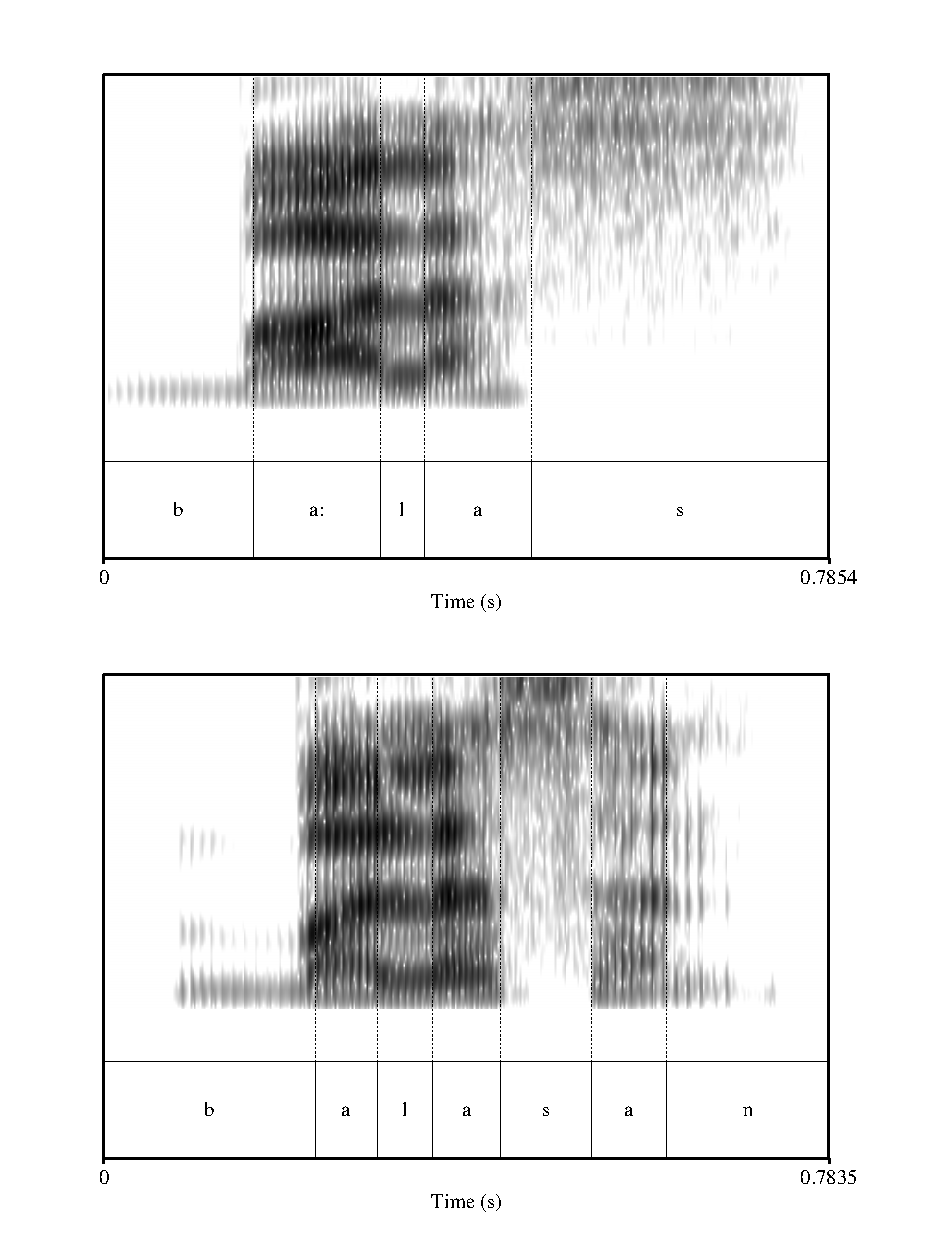
\includegraphics{pics/baalasbalasan.eps}
 % baalasbalasan.eps: 1310738x1179666 pixel, 0dpi, infxinf cm, bb=
 \caption[Absence of vowel lengthening after derivation]{The word \phontrs{ba:las}{answer(v)} has a long first vowel (138ms). This same vowel is realized as short (67ms) upon the addition of the nominalizing suffix \em -an \em.}
 \label{fig:baalasbalasan}
\end{figure}



There is one additional structure for stems which is never found in roots, namely

\begin{itemize}
 \item C\E.CV.CVC e.g. \phontrs{sIgaR-an}{healthy'+`\textsc{nmlzr}'=`health}, where the schwa is always realized as \phonet{I}.
\end{itemize}

This structure has no long vowel, but a raised schwa in the first syllable. This stem structure contrasts with the structure of trisyllabic roots, where a schwa in the initial syllable  triggers a long vowel in the penultimate. Additionally, schwa in trisyllabic roots is always realized as \phonet{@}, while here it is never realized as \phonet{\E}, but always as \phonet{I}.




The second category-changing suffix next to the nominalizer \em -an \em mentioned above is the causativizer \em -ki\ng\em, which can behave like \em -an \em in making a word trisyllabic, resulting in a short vowel. The behaviour of \em -ki\ng{} \em is a bit more complex though and is treated in more detail on page \pageref{page:phon:king}.

Similar behaviour is found for the numeral derivational suffixes \phontrs{-blas}{-teen} and \phontrs{-pulu}{-ty}, which disallow long vowels.

The   derivational prefixes, \phontrs{ka-}{\textsc{ord}} and \phontrs{k@n@-}{\textsc{invol}}, do not have any influence on the vowel length of their host.

Compound stems like \phontrs{kaca ma:\dentt a}{mirror+eye=spectacles} can only have long vowels in the last part of the compound. This is true for nominal compounds like \phonet{kaca ma:\dentt a}, but also for verbal compounds like \phontrs{kasi ka:\V i\ng}{give+marry=marry off}.


% \xbox{14}{
% \ea \label{ex:form:modals:mau:recipe}
% \gll manis-an=nang mà-thaaro guula \textbf{maau} gula paasir konnyong \textbf{maau} \\
%  sweet-\textsc{nmlzr}=\textsc{dat} \textsc{inf}-put sugar want sugar sand few want\\
% `In order to make it sweet, you need sugar, you need a bit of crystal sugar.' (B060115rcp02)
% \z
% }


\subsection{Words}\label{sec:phon:struct:Words}
The structure of stems is not changed by adding additional material on the word level, such as inflectional affixes or clitics. For instance, the quantity of the vowels remains the same if a clitic like \phontrs{=pe}{\textsc{poss}} is attached to the stem, e.g. \phontrs{ba:pa}{father}, \phontrs{ba:pa=pe}{father's} with a long vowel in both, or \phontrs{makanan=pe}{of the food}, with a short vowel as in \phonet{makanan}\#. An inflectional suffix like the imperative \em -la \em would   not change the vowel quantity of the stem it attaches to, either.

\subsection{Word length}\label{sec:phon:Wordlength}
Disyllabic roots are most common (ca. 90\%), while trisyllabic roots are more rare (ca. 10\%). Only a handful of lexical roots consists of one syllable: \phontrs{pii}{go}, \phontrs{pon}{bride}, \phontrs{\dentt e:}{tea},  and \phontrs{ca:}{tea}, besides the function words \phontrs{se:}{1s.polite}, \phontrs{go:}{1s}{familiar}, \phontrs{lu:}{2s.familiar},  and \phontrs{de:}{3s.familiar}. More than three syllables are found in the words  \phontrs{kenija:ja}{in vain} and \phontrs{bukaRijOk}{cock-a-doodle-do}. %demikian

By affixation and compounding, longer words can be formed, but more than five syllables are rarely found. The longest \em bona fide \em word (i.e. without clitics) found up to now is \phontrs{k@-sbilan-pulu}{nintieth}. If clitics are included, there is technically no longest word because clitics can be stacked infinitely (see Section \ref{sec:morph:Boundwords}, p. \pageref{sec:morph:Boundwords}).



\subsection{Syllable prominence}\label{sec:phon:Syllableprominence}
Sri Lanka Malay words do not show different levels of prominence in their syllables, neither phonologically nor phonetically. In other words, there is no word accent or stress. \citet{SmithEtAl2004} claim that ``stress falls on the long vowel of a word, or on the initial syllable if the word only contains only short vowels.'' They do not state by which acoustic cue they established the location of stress, so that we are probably dealing with an impressionistic statement here. \citet{Bakker2006} reports accent on the first syllable, drawing on \citet{Robuchon2003}. These statements again seem to be impressionistic. Some instrumental analyses were undertaken to check these claims, but no cues for a saliently prominent (stressed) syllable could be found. 49 words with different syllable structures were checked in 6 different controlled environments with two male native speakers of SLM for pitch contour and intensity. The compiled measurements taken together do not suggest that a meaningful generalization about the correlation between word structure and  pitch or intensity can be made  \citep{ApoussidouEtAl2008}.

\begin{figure}
 \centering
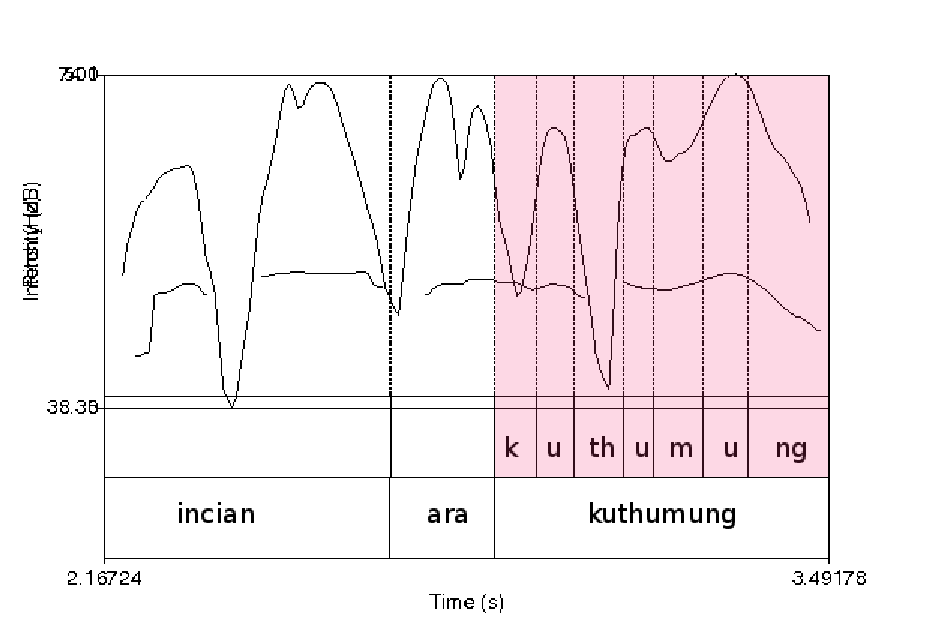
\includegraphics{pics/kuthumungintenspitch.eps}
%  kuthumung-spectro.png: 432x252 pixel, 72dpi, 15.24x8.89 cm, bb=0 0 432 252
 \caption[Absence of pitch and intensity cues for stress in the word \phontrs{ku\dentt umuN}{see}]{Pitch and intensity of an utterance involving the word \phontrs{ku\dentt umuN}{see} show that the first two syllables are not very different in intensity and pitch. Intensity and pitch cannot be used to determine which of the two should be the head. The final syllable has a higher loudness and a raise-fall pitch movement, both of which are the usual way of indicating utterance boundaries of declaratives.}
\label{fig:kuthumungintenspitch}
\end{figure}



Figure \ref{fig:kuthumungintenspitch} shows that neither pitch nor intensity distinguish the first two syllables from each other in the trisyllabic word \phontrs{ku\dentt umu\ng}{see}(The effects on the final syllable are due to the utterance boundary).\footnote{I am aware of the fact that the historical source for this word had two schwas in the first two syllables, so that the lower intensity could be attributed to that.  I do not think that this word has a synchronic schwa, though. The reason for this is that it behaves exactly like trisyllabic words without schwa like \phontrs{makanan}{food}. This word was chosen because it is a monomorphemic trisyllable, of which there are not many. Polymorphemic trisyllables are easier to come by, e.g. nominalizations with \em -an\em. These polymorphemic words were not retained for the recording session  in order to avoid influences that the affixes might have on stress placement. In hindsight, this was a mistake. Future research should include some of these affixes trisyllables as well. I am confident that future research on pitch and intensity will provide no more stress cues for these trisyllables than they did for disyllables or the \textipa{ku\dentt umuN}-type words.} Instrumental analysis of a sample of words with different syllable structures in varying positions within the clause showed that \em ku\dentt umu\ng{} \em is no exception and that pitch and intensity do not provide cues of prominence \citep{ApoussidouEtAl2008}. This lack of word accent is actually not unheard of in the Malay world, as will be discussed in more detail in Section \ref{sec:phon:SLMasastresslesslanguage}.
Another stress cue which some languages use to indicate prominence of a syllable is vowel duration. This is not the case in SLM either. The spectrogram of \em ku\dentt umu\ng{} \em (Figure \ref{fig:kuthumungspectro}) shows that the vowels are of comparable length here (also see Figure \ref{fig:baalasbalasan} for a derived trisyllable). True, there are long and short vowels in SLM, as shown in Section \ref{sec:phon:Vowellength}, but if this was a stress cue, we would expect a difference in vowel duration (or at least moraic weight) to show up in every word, namely on the prominent syllable. This is not the case, as words like \em ku\dentt umu\ng{} \em show. The hypothesis makes wrong predictions, and must be amended or abandoned. A possible amendment would be to state \em Trisyllables of the \em ku\dentt umu\ng{} \em type do not show stress. \em This amendment would have to rely on lexical specification. The fact that there are differences in vowel duration needs explanation nevertheless. In Section \ref{sec:phon:Analysisofwordstructure}, I will argue that vowel duration can better be explained by foot structure, and that this analysis does not need specification in the lexicon and is therefore superior to the ``stress analysis''.


\begin{figure}
 \centering
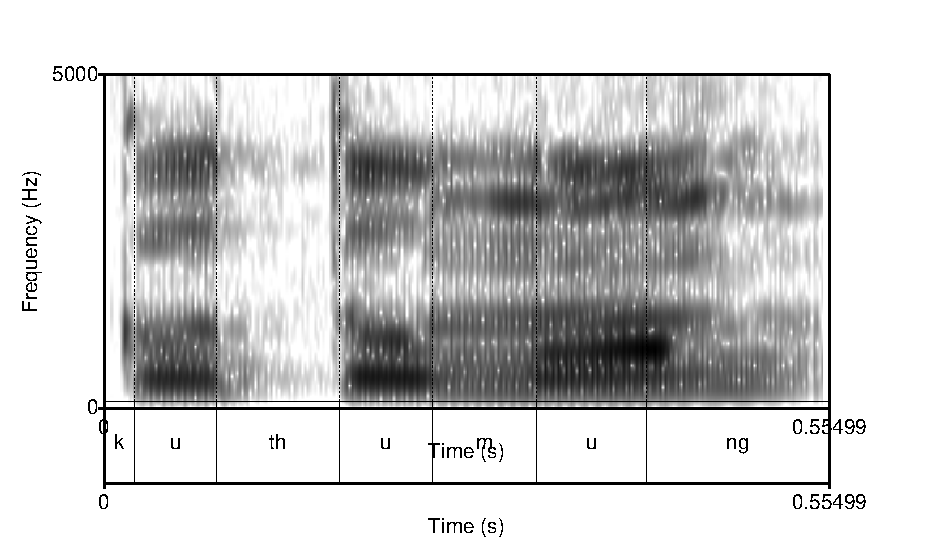
\includegraphics{pics/kuthumung-spectro.eps}
%  kuthumung-spectro.png: 432x252 pixel, 72dpi, 15.24x8.89 cm, bb=0 0 432 252
 \caption[Duration of vowels in \phontrs{ku\dentt umuN}{see}]{The spectrogram of \phontrs{ku\dentt umuN}{see} shows that all three u's are of about equal duration. Duration is therefore not a cue to determine syllable prominence.}
\label{fig:kuthumungspectro}
\end{figure}


The last stress cue which some languages use is vowel quality. Prominent syllables typically show a greater range of possible vowels, whereas non-prominent syllables have a smaller array and might only admit reduced vowels. In SLM, the antepenultimate syllable  of a root seems to be a less prominent syllable, since it only admits  [i], [u] and schwa (the latter often dropped altogether), but not [a], [e] or [o], the most sonorant vowels \citep{Jespersen1904,Selkirk1984,Clements1990sonority}.\footnote{Antepenultimate syllables are often restricted to schwa in Malay varieties, see \citet[12,31,59]{Adelaar1985} for examples of Standard Malay and Jakartanese.} While this is an indication of lack of prominence of this syllable, it does not indicate which of the remaining syllables is most prominent. Furthermore, this lack of prominence of the antepenultimate only applies on the root level; on the stem level, any vowel can be found in antepenultimate position (see Section \ref{sec:phon:struct:Stems}).

To conclude, pitch and intensity do not distinguish syllable prominence in SLM. Differences in vowel duration are not found in all words and are therefore a bad stress cue. Vowel quality finally could indicate lack of prominence of one syllable on the root level. It does not provide positive prominence cues on the stem level, and does not provide any cues on the stem level.


\section{Analysis of word structure}\label{sec:phon:Analysisofwordstructure}
I will argue in this section that the different types of roots we find in SLM and the occurrence of long vowels can be explained by extrametricality of the final syllable \citep{Kiparsky1985lexphon} and a bimoraic foot requirement\footnote{It is interesting to note that Sinhala also parses words into bimoraic feet \citep{Letterman1997}.} \citep{McCarthyEtAl1993}. The list in \xref{list:phon:wordtypes} is repeated and reordered here for convenience.



\setcounter{mycounter}{1}
\ea\label{list:phon:wordtypes2}
\begin{tabular}{@{\arabic{mycounter})\stepcounter{mycounter}~~~~~}ll@{~~~e.g.~~~}l}
&(C)VC$_i$.C$_j$V(C)	 & \phontrs{kumpul}{collect}\\
&(C)VC$_i$.C$_i$V(C)	 & \phontrs{\dentt op:i}{hat}\\
&CV.CV.CV(C)		 & \phontrs{ku\dentt umu\ng}{see}\\
&(C)V\textipa{:}.CV(C)		 & \phontrs{\dentt i:ga}{three}\\
&CV\textipa{:}.GVC		 & \phontrs{\dentt u:\V a}{old} (G=glide)\\
&C\E.CV\textipa{:}.CV(C)		 & \phontrs{c\E ca:\V ak}{wash}\\
&C\E C$_i$.C$_j$V	& \phontrs{m\I \dentn\dentt a}{vomit}\\
&(C)\E C$_j$.C$_j$V(C)	 & \phontrs{s\I g:aR}{healthy}\\
&CV\textipa{:}			 & \phontrs{pi:}{go}, \phontrs{\dentt e:}{tea}\\
&CVC			 & \phontrs{pon}{bride}\\
&(C)V.CV			 & \phontrs{ka\dentt a}{\textsc{quot}}\\
&CVC.CVC.CVC		 & \phontrs{kak:aRla\dentt}{cockroach} (only example)\\

&CV.GVC		 	& \phontrs{lija\dentt}{see}\\

&CV$_i$.h$_i$C		 & \phontrs{poho\ng}{tree}\\
&(\E)N.CVC		 & \phontrs{(\U)mpa\dentt}{four}\\
&(\E)C$_i$.C$_i$V(C)	 & \phontrs{(\U)m:as}{gold}\\
\end{tabular}
\z


\subsection{Roots}\label{sec:phon:analysis:Roots}

The following analytic generalizations can be drawn from this list: Within stems, a penultimate syllable is heavy iff it is not preceded by another syllable containing a full vowel, where heavy syllables are CV\textipa{:} and CVC. I propose that this distribution can be captured by the following principles:

\begin{itemize}
 \item treat final syllables as extrametrical 
 \item build bimoraic feet at right edge of stem
 \item \E{} cannot project a mora \citep{Kager1989}
 \item \I{} and \U{} can project a mora
 \item reduced vowels \phonet{@,I,U} cannot lengthen
\end{itemize}

From these principles, it follows that disyllabic stems lengthen the vowel in an open penultimate syllable to build a bimoraic foot. The same is true for trisyllables with initial schwa. This will be developed below for the different types.

\subsubsection{Canonical cases}\label{sec:phon:Canonicalcasesroots}

A straightforward example of the internal structure of the root is /kumpul/`collect'. This is parsed as /(ku$_{\mu}$m$_{\mu})<$pul$>$/, whose representation is given in \xref{ex:phon:rep:miskin}.

\ea\label{ex:phon:rep:miskin}
\begin{tabular}{lll}
 & ~~~~~~~~~$\omega$\\
 & ~~~~~~/&~ \begin{picture}(0,0)\put(-10,8){\line(1,-3){13}}\end{picture}\\
 & ~~~~F   &  \\
 & ~~~/   &  \\
 &$\sigma$    &$<\sigma>$ \\
 & $\mid$~$\backslash$    & \\
 & $\mu$~$\mu$   &\\
% %  & $\mid$~~~$\mid$&    $\mid$~~~~$\mid$ \\
% C\begin{picture}(0,0)\put(0,10){\line(1,5){8}}\end{picture} & VC~~~C\begin{picture}(0,0)\put(0,10){\line(1,5){8}}\end{picture}   & V  C \\
 & $\mid$~~~$\mid$ & \\
k\begin{picture}(0,0)\put(0,10){\line(1,5){8}}\end{picture} &u~m
&
p\begin{picture}(0,0)\put(-2,10){\line(1,5){8}}\end{picture}
~u\begin{picture}(0,0)\put(-2,10){\line(0,5){40}}\end{picture}
~l\begin{picture}(0,0)\put(-2,10){\line(-1,5){8}}\end{picture}\\
\end{tabular}
\z

We exclude the final syllable \em pul \em and parse the remaining syllable \em kum \em in a bimoraic foot, where the vowel and the coda consonant contribute one mora each.

For disyllables with an underlying geminate, such as \phontrs{\dentt op:i}{hat}, the representation is similar, but the coda consonant of the first syllable serves at the same time as onset of the final syllable.

\ea\label{ex:phon:rep:thoppi}
\begin{tabular}{lll}
 & ~~~~~~~$\omega$\\
 & ~~~~~~/&~ \begin{picture}(0,0)\put(-20,8){\line(1,-3){13}}\end{picture}\\
 & ~~~~F   &  \\
 & ~~~/   &  \\
 &$\sigma$    &\hspace{-0.3cm}$<\sigma>$ \\
 & $\mid$~$\backslash$    & \\
 & $\mu$~$\mu$   &\\
% %  & $\mid$~~~$\mid$&    $\mid$~~~~$\mid$ \\
% C\begin{picture}(0,0)\put(0,10){\line(1,5){8}}\end{picture} & VC~~~C\begin{picture}(0,0)\put(0,10){\line(1,5){8}}\end{picture}   & V  C \\
 & $\mid$~~~~$\backslash$ & \\
\dentt\begin{picture}(0,0)\put(0,10){\line(1,5){8}}\end{picture} & o~~~~~p\begin{picture}(0,0)\put(0,10){\line(1,3){13}}\end{picture}
&
i\begin{picture}(0,0)\put(-2,10){\line(0,5){40}}\end{picture}\\
\end{tabular}
\z


Trisyllabic words like \phontrs{ku\dentt umu\ng}{see} have the foot stretching over two syllables.

\ea\label{ex:phon:rep:kuthumung}
\begin{tabular}{ccc}
 & $\omega$\\
 & /~~~~~& \begin{picture}(0,0)\put(-28,8){\line(2,-3){25}}\end{picture}\\
\multicolumn{2}{c}{~~~~F}&\\
~~~~~/&$\backslash$&\\
~~$\sigma$&~~$\sigma$&$<\sigma>$   \\
~~$\mid$&~~$\mid$&\\
~~~$\mu$&~~~$\mu$&\\
 ~~$\mid$&~~~$\mid$&\\
k\begin{picture}(0,0)\put(-4,10){\line(1,6){7}}\end{picture}~~u &
\dentt\begin{picture}(0,0)\put(-4,10){\line(1,6){7}}\end{picture}~~u&
m\begin{picture}(0,0)\put(-2,10){\line(1,5){8}}\end{picture}
~u\begin{picture}(0,0)\put(-2,10){\line(0,5){40}}\end{picture}
~\ng\begin{picture}(0,0)\put(-2,10){\line(-1,5){8}}\end{picture}\\
\end{tabular}
\z

In disyllables without coda consonant in the penultimate, like \phontrs{\dentt i:ga}{three} \xref{ex:phon:rep:thiiga}, the vowel is lengthened to contribute the second mora for the bimoraic foot.

\ea\label{ex:phon:rep:thiiga}
\begin{tabular}{lll}
 & ~~~~~~~~~$\omega$\\
 & ~~~~~~/&~ \begin{picture}(0,0)\put(-10,8){\line(1,-3){13}}\end{picture}\\
 & ~~~~F   &  \\
 & ~~~/   &  \\
 &$\sigma$    &$<\sigma>$ \\
 & $\mid$~$\backslash$    & \\
 & $\mu$~$\mu$   &\\
% %  & $\mid$~~~$\mid$&    $\mid$~~~~$\mid$ \\
% C\begin{picture}(0,0)\put(0,10){\line(1,5){8}}\end{picture} & VC~~~C\begin{picture}(0,0)\put(0,10){\line(1,5){8}}\end{picture}   & V  C \\
 & $\backslash$~/ & \\
\dentt\begin{picture}(0,0)\put(0,10){\line(1,5){8}}\end{picture}&
 ~~i&
g\begin{picture}(0,0)\put(-2,10){\line(1,5){8}}\end{picture}
~a\begin{picture}(0,0)\put(-2,10){\line(0,5){40}}\end{picture}\\
\end{tabular}
\z

For one set of lexemes with a glide as the onset of the final syllable, the representation is the same as for \phonet{\dentt i:ga}, just above. The word \phontrs{\dentt u:\V a}{old} has an identical representation \xref{ex:phon:rep:thuuva} to \phonet{\dentt i:ga} above.\footnote{This contrasts with a more problematic case for \phontrs{\dentt u\V an}{gentleman}, shown below in \xref{ex:phon:rep:thuvan}.}

\ea\label{ex:phon:rep:thuuva}
\begin{tabular}{lll}
 & ~~~~~~~~~$\omega$\\
 & ~~~~~~/&~ \begin{picture}(0,0)\put(-10,8){\line(1,-3){13}}\end{picture}\\
 & ~~~~F   &  \\
 & ~~~/   &  \\
 &$\sigma$    &$<\sigma>$ \\
 & $\mid$~$\backslash$    & \\
 & $\mu$~$\mu$   &\\
% %  & $\mid$~~~$\mid$&    $\mid$~~~~$\mid$ \\
% C\begin{picture}(0,0)\put(0,10){\line(1,5){8}}\end{picture} & VC~~~C\begin{picture}(0,0)\put(0,10){\line(1,5){8}}\end{picture}   & V  C \\
 & $\backslash$~/ & \\
\dentt\begin{picture}(0,0)\put(0,10){\line(1,5){8}}\end{picture}&
 ~~u&
\V\begin{picture}(0,0)\put(-2,10){\line(1,5){8}}\end{picture}
~a\begin{picture}(0,0)\put(-2,10){\line(0,5){40}}\end{picture}\\
\end{tabular}
\z

In trisyllables with an initial schwa and an open penultimate like \phontrs{c\E ca:\V ak}{wash}, the vowel in the penultimate is also lengthened. This indicates that \E{} does not project a mora \citep[cf.][]{Kager1989}. The foot is then constructed only with the material of the penultimate syllable, which means that the vowel of this syllable needs to be lengthened.

\ea\label{ex:phon:rep:cEcaavak}
	\begin{tabular}{llll}
	& ~~~~$\omega$\\
	& \begin{picture}(0,0)\put(8,8){\line(-1,-2){20}}\end{picture}~~~~~$\mid$&    \begin{picture}(0,0)\put(-10,8){\line(1,-2){20}}\end{picture}\\
	\multicolumn{2}{r}{F~~~~}&\\
		& ~~~~$\mid$ \\
	~~~~$\sigma$ & ~~~~$\sigma$&$<\sigma>$   \\
	& ~~~~$\mid$~$\backslash$    & \\
	& ~~~~$\mu$~$\mu$   & \\
	& ~~~ $\backslash$~/&\\
c\begin{picture}(0,0)\put(-2,10){\line(1,5){8}}\end{picture}
~\E\begin{picture}(0,0)\put(-2,10){\line(0,5){40}}\end{picture}&
c\begin{picture}(0,0)\put(-4,10){\line(1,5){8}}\end{picture}
~~a &
\V\begin{picture}(0,0)\put(-2,10){\line(1,5){8}}\end{picture}
~a\begin{picture}(0,0)\put(-2,10){\line(0,5){40}}\end{picture}
~k\begin{picture}(0,0)\put(-2,10){\line(-1,5){8}}\end{picture}\\
	\end{tabular}
\z

If schwa occurs in a disyllabic like \phontrs{m\I \dentn\dentt a}{ask}, schwa is realized as \I{}, which, unlike \E,  can project a mora. This raising of schwa is then a result of the need for an additional mora, since the coda consonant (in this case /n/)  only provides one, not enough to construct a bimoraic foot.


\ea\label{ex:phon:rep:mIntha}
\begin{tabular}{lll}
 & ~~~~~~~~~$\omega$\\
 & ~~~~~~/&~ \begin{picture}(0,0)\put(-10,8){\line(1,-3){13}}\end{picture}\\
 & ~~~~F   &  \\
 & ~~~/   &  \\
 &$\sigma$    &$<\sigma>$ \\
 & $\mid$~$\backslash$    & \\
 & $\mu$~$\mu$   &\\
% %  & $\mid$~~~$\mid$&    $\mid$~~~~$\mid$ \\
% C\begin{picture}(0,0)\put(0,10){\line(1,5){8}}\end{picture} & VC~~~C\begin{picture}(0,0)\put(0,10){\line(1,5){8}}\end{picture}   & V  C \\
 & $\mid$~~~$\mid$ & \\
m\begin{picture}(0,0)\put(0,10){\line(1,5){8}}\end{picture} & \I~~~\dentn
&
\dentt\begin{picture}(0,0)\put(-2,10){\line(1,5){8}}\end{picture}
~a\begin{picture}(0,0)\put(-2,10){\line(0,5){40}}\end{picture}\\
\end{tabular}
\z

If the initial syllable of a disyllabic word contains schwa in an open syllable, moraic content is neither present in the vowel, since \E{} does not have moraic content, nor in the coda, which is absent. In this case, two things happen: \E{} is raised to \I{}, which does project one mora, and the onset of the following syllable is geminated, yielding a coda, and thereby an additional mora.

\ea\label{ex:phon:rep:sIggar}
\begin{tabular}{lll}
 & ~~~~~~~$\omega$\\
 & ~~~~~~/&~ \begin{picture}(0,0)\put(-20,8){\line(1,-3){13}}\end{picture}\\
 & ~~~~F   &  \\
 & ~~~/   &  \\
 &$\sigma$    &\hspace{-0.3cm}$<\sigma>$ \\
 & $\mid$~$\backslash$    & \\
 & $\mu$~$\mu$   &\\
% %  & $\mid$~~~$\mid$&    $\mid$~~~~$\mid$ \\
% C\begin{picture}(0,0)\put(0,10){\line(1,5){8}}\end{picture} & VC~~~C\begin{picture}(0,0)\put(0,10){\line(1,5){8}}\end{picture}   & V  C \\
 & $\mid$~~~~$\backslash$ & \\
s\begin{picture}(0,0)\put(0,10){\line(1,5){8}}\end{picture} & \I~~~~~g\begin{picture}(0,0)\put(0,10){\line(1,2){20}}\end{picture}
&
a\begin{picture}(0,0)\put(-2,10){\line(0,5){40}}\end{picture}
~r\begin{picture}(0,0)\put(-2,10){\line(-1,5){8}}\end{picture}\\
\end{tabular}
\z



There are only a handful of monosyllabic lexical words such as \phontrs{pi:}{go}, \phontrs{pon}{bride} and \phontrs{\dentt aj}{excrement}. Additionally, there are the pronouns \phontrs{se:}{\textsc{1s.polite}}, \phontrs{go:}{\textsc{1s.familiar}},  \phontrs{lu:}{\textsc{2s.familiar}},  \phontrs{de:}{\textsc{3s.familiar}}.
The fact that all monosyllables have a heavy syllable, especially the long vowel in \textipa{pi:} suggests that the final syllable is not treated as extrametrical for these words. Instead, the bimoraic foot is constructed over the whole word.


\xbox{5}{
\ea\label{ex:phon:rep:pii}
\begin{tabular}{ccc}
 &$\omega$\\
 &$\mid$&\\
 &F   &  \\
 & $\mid$ &  \\
 &$\sigma$    &  \\
 & $\mid$~$\backslash$    & \\
 & $\mu$~$\mu$   &\\
% %  & $\mid$~~~$\mid$&    $\mid$~~~~$\mid$ \\
% C\begin{picture}(0,0)\put(0,10){\line(1,5){8}}\end{picture} & VC~~~C\begin{picture}(0,0)\put(0,10){\line(1,5){8}}\end{picture}   & V  C \\
 & $\backslash$~/ & \\
p\begin{picture}(0,0)\put(0,10){\line(1,4){10}}\end{picture}&
 ~~i&\\
\end{tabular}
\z
} 
\xbox{5}{
\ea\label{ex:phon:rep:pon}
\begin{tabular}{ccc}
 &$\omega$\\
 &$\mid$&\\
 &F   &  \\
 & $\mid$ &  \\
 &$\sigma$    &  \\
 & $\mid$~$\backslash$    & \\
 & $\mu$~$\mu$   &\\
% %  & $\mid$~~~$\mid$&    $\mid$~~~~$\mid$ \\
% C\begin{picture}(0,0)\put(0,10){\line(1,5){8}}\end{picture} & VC~~~C\begin{picture}(0,0)\put(0,10){\line(1,5){8}}\end{picture}   & V  C \\
 & $\mid$~~~$\mid$ & \\
p\begin{picture}(0,0)\put(0,10){\line(1,4){10}}\end{picture}&
o~~n&\\
\end{tabular}
\z
} \\

No function word has a long vowel, even not in penultimate open syllables. This suggests that function words are not subject to the bimoraic foot requirement, and are probably not parsed into a foot nor a word. \xref{ex:phon:rep:katha} shows this for the quotative \em ka\dentt a\em. In this representation, the levels of word, foot and mora are left out, since they are irrelevant for the word \em ka\dentt a\em. 

\xbox{7}{
\ea\label{ex:phon:rep:katha}
\begin{tabular}{cc}
~~  $\sigma$ &~$\sigma$\vspace{0,3cm} \\\\\\
k \begin{picture}(0,0)\put(-2,10){\line(1,5){8}}\end{picture}
~~ 
~a\begin{picture}(0,0)\put(-2,10){\line(-1,5){8}}\end{picture}
&
\dentt \begin{picture}(0,0)\put(-2,10){\line(1,5){8}}\end{picture}
~~ 
~a\begin{picture}(0,0)\put(-2,10){\line(-1,5){8}}\end{picture}\\
\end{tabular}
\z
}


Trisyllabic roots with closed syllables are rare. Only one could be found, \phontrs{kak:aRla\dentt}{cockroach}. It is not clear as of now whether this root is parsed into one bimoraic foot, disregarding the first syllable \xref{ex:phon:rep:kakkarlath1}, or into two feet, as in \xref{ex:phon:rep:kakkarlath2}.



\xbox{7}{
\ea\label{ex:phon:rep:kakkarlath1}
\begin{tabular}{lll}
  	& ~~~$\omega$\\
	&\begin{picture}(0,0)\put(3,8){\line(-1,-2){20}}\end{picture}~~~~$\mid$~~~~~& \begin{picture}(0,0)\put(-23,8){\line(2,-3){25}}\end{picture}\\
~~~~~~~~ &~~~~F&\\
~~~~~~~&  ~~~~$\mid$&\\
~~~~~$\sigma$&~~~~$\sigma$&$<\sigma>$   \\
&~~~~$\mid$ $\backslash$&\\
&~~~~$\mu$~~$\mu$&\\
&~~~ $\mid$~~~$\mid$&\\

k\begin{picture}(0,0)\put(-2,10){\line(1,5){8}}\end{picture}
~a\begin{picture}(0,0)\put(-2,10){\line(0,5){40}}\end{picture}
 &
k\begin{picture}(0,0)\put(-7,10){\line(-1,2){20}}\put(-5,10){\line(1,6){7}}\end{picture}~
a~~r&
l\begin{picture}(0,0)\put(-2,10){\line(1,5){8}}\end{picture}
~a\begin{picture}(0,0)\put(-2,10){\line(0,5){40}}\end{picture}
~\dentt\begin{picture}(0,0)\put(-2,10){\line(-1,5){8}}\end{picture}\\
\end{tabular}
\z
} 
\xbox{7}{
\ea\label{ex:phon:rep:kakkarlath2}
\begin{tabular}{lll}
  	& ~~$\omega$\\
	&\begin{picture}(0,0)\put(-2,8){\line(-2,-3){8}}\end{picture}~~~~$\mid$~~~~~& \begin{picture}(0,0)\put(-23,8){\line(2,-3){25}}\end{picture}\\
~~~~~~~~F &~~~~F&\\
~~~~~~~/&  ~~~~$\mid$&\\
~~~~~$\sigma$&~~~~$\sigma$&$<\sigma>$   \\
~~~~~$\mid$ $\backslash$&~~~~$\mid$ $\backslash$&\\
~~~~$\mu$~$\mu$&~~~~$\mu$~~$\mu$&\\
~~~~~$\mid$&~~~ $\mid$~~~$\mid$&\\
k\begin{picture}(0,0)\put(-2,10){\line(1,6){7}}\end{picture}~~
a &
k\begin{picture}(0,0)\put(-7,10){\line(-1,1){14}}\put(-5,10){\line(1,6){7}}\end{picture}~
a~~r&
l\begin{picture}(0,0)\put(-2,10){\line(1,5){8}}\end{picture}
~a\begin{picture}(0,0)\put(-2,10){\line(0,5){40}}\end{picture}
~\dentt\begin{picture}(0,0)\put(-2,10){\line(-1,5){8}}\end{picture}\\
\end{tabular}
\z
}

\subsubsection{Problematic cases}\label{sec:phon:Problematiccases}


A more problematic case for this analysis are co-occurrence of empty coda and empty onset. Our analysis would predict that for words of the form /CV$_i$V$_j$C/, we get [CV$_i$:V$_j$C] \xref{ex:phon:rep:liiath}. However, what we find is [CV$_i$GV$_j$C] where G is a glide. This newly formed glide is  resyllabified to the onset of the following syllable, yielding [CV$_i$.GV$_j$C]. This resyllabification means that the glide can no longer be the coda, unless it is geminated, which is not the case here. With the coda disappearing, the mora also goes, leaving insufficient material to construct a foot. This is illustrated in \xref{ex:phon:rep:liiath} and \xref{ex:phon:rep:thuuan}.


\xbox{7}{
\ea\label{ex:phon:rep:liiath}*
\begin{tabular}{ll}
 & ~~~~~~$\omega$\\
 & ~~~~~~/~ \begin{picture}(0,0)\put(0,8){\line(1,-3){13}}\end{picture}\\
 & ~~~~F     \\
 & ~~~/     \\
 &$\sigma$ ~~~~ $<\sigma>$ \\
 & $\mid$~$\backslash$     \\
 & $\mu$~$\mu$   \\
 & ~$\backslash$  $\mid$  \\
~*l\begin{picture}(0,0)\put(0,10){\line(1,5){8}}\end{picture}&
 ~~~
i~
~~~~~a\begin{picture}(0,0)\put(-2,10){\line(0,5){40}}\end{picture}
~\dentt\begin{picture}(0,0)\put(-2,10){\line(-1,5){8}}\end{picture}~~(=\phonet{li:a\dentt})\\
\end{tabular}
\z
}
\xbox{7}{
\ea\label{ex:phon:rep:liyath}
\begin{tabular}{ll}
 & ~~~~~~$\omega$\\
 & ~~~~~~/~ \begin{picture}(0,0)\put(0,8){\line(1,-3){13}}\end{picture}\\
 & ~~~~F?     \\
 & ~~~/     \\
 &$\sigma$ ~~~~ $<\sigma>$ \\
 & $\mid$~?     \\
 & $\mu$~$\mu$?   \\
 & ~$\backslash$  ?  \\
l\begin{picture}(0,0)\put(0,10){\line(1,5){8}}\end{picture}&
 ~~~
i~\begin{picture}(0,0)\put(0,12){\line(2,5){15}}\end{picture}
~~~~~a\begin{picture}(0,0)\put(-2,10){\line(0,5){40}}\end{picture}
~\dentt\begin{picture}(0,0)\put(-2,10){\line(-1,5){8}}\end{picture}~~(=\phonet{lija\dentt})\\
\end{tabular}
\z
}

\xbox{7}{
\ea\label{ex:phon:rep:thuuan}*
\begin{tabular}{ll}
 & ~~~~~~$\omega$\\
 & ~~~~~~/~ \begin{picture}(0,0)\put(0,8){\line(1,-3){13}}\end{picture}\\
 & ~~~~F     \\
 & ~~~/     \\
 &$\sigma$ ~~~~ $<\sigma>$ \\
 & $\mid$~$\backslash$     \\
 & $\mu$~$\mu$   \\
 & ~$\backslash$  $\mid$  \\
~*\dentt\begin{picture}(0,0)\put(0,10){\line(1,5){8}}\end{picture}&
 ~~~
u~
~~~~~a\begin{picture}(0,0)\put(-2,10){\line(0,5){40}}\end{picture}
~n\begin{picture}(0,0)\put(-2,10){\line(-1,5){8}}\end{picture}~~(=\phonet{\dentt u:an})\\
\end{tabular}
\z
}
\xbox{7}{
\ea\label{ex:phon:rep:thuvan}
\begin{tabular}{ll}
 & ~~~~~~$\omega$\\
 & ~~~~~~/~ \begin{picture}(0,0)\put(0,8){\line(1,-3){13}}\end{picture}\\
 & ~~~~F?     \\
 & ~~~/     \\
 &$\sigma$ ~~~~ $<\sigma>$ \\
 & $\mid$~?     \\
 & $\mu$~$\mu$?   \\
 & ~$\backslash$  ?  \\
\dentt\begin{picture}(0,0)\put(0,10){\line(1,5){8}}\end{picture}&
 ~~~
u~\begin{picture}(0,0)\put(0,12){\line(2,5){15}}\end{picture}
~~~~~a\begin{picture}(0,0)\put(-2,10){\line(0,5){40}}\end{picture}
~n\begin{picture}(0,0)\put(-2,10){\line(-1,5){8}}\end{picture}~~(=\phonet{\dentt u\V an})\\
\end{tabular}
\z
}





Under derivational accounts, it is easy to formulate a rule like
% 
% \ea $\begin{array}{c}[+vocalic]\\[\pm front]\end{array}:\to\begin{array}{c}[+vocalic]\\[\pm front]\end{array}\begin{array}{c}[-vocalic]\\[\pm front]\end{array}$\_V\z

\ea $[+vocalic]$\textipa{:}$ \to [+vocalic][-vocalic]/\_[+vocalic]$\z

In other words, a long vowel is split into a vowel and a glide before another vowel. It is unclear as of now how this could be made to work with the general foot structure.

The problem with words of the structure CV$_i$.hV$_i$C	like \phontrs{poho\ng}{tree} is similar. A vowel preceding the same vowel, separated by an /h/ is never lengthened. \citet{Tapovanaye1995} assumes that these words have the underlying form /CV$_i$V$_i$C/ and that an h is inserted to prevent hiatus. Crucially, this takes place after vowel lengthening. In such a derivational account, this can be formulated as

\ea V$_i$\textipa{:} $\to$ V$_i$h/\_V$_i$\z

This phenomenon cannot be captured with the analysis presented there. The bimoraic foot cannot be constructed for these words. On the other hand, the derivational account presented by Tapovanaye is not very plausible either, since the insertion of an h instead of a glide is not very well motivated, and historically, an h is present in these words anyway. 

Another problem for the foot structure assumed in this analysis is the deletion of schwa between empty onset and nasals as in \phonem{@mpa\dentt}, which can be pronounced \phonet{Umpa\dentt}, but also \phonet{\s{m}pa\dentt}. For the first pronunciation, there is no problem \xref{ex:phon:rep:umpath}, but if the raised schwa is deleted, as is the case in the second pronunciation, a mora disappears and no bimoraic foot can be constructed. Whether the final syllable should be extrametrical \xref{ex:phon:rep:mpath1} or not \xref{ex:phon:rep:mpath2} is unclear as of now.



\xbox{5}{
\ea\label{ex:phon:rep:umpath}
\begin{tabular}{lll}
 & ~~~~~~~~~$\omega$\\
 & ~~~~~~/&~ \begin{picture}(0,0)\put(-10,8){\line(1,-3){13}}\end{picture}\\
 & ~~~~F   &  \\
 & ~~~/   &  \\
 &$\sigma$    &$<\sigma>$ \\
 & $\mid$~$\backslash$    & \\
 & $\mu$~$\mu$   & \\
% %  & $\mid$~~~$\mid$&    $\mid$~~~~$\mid$ \\
% C\begin{picture}(0,0)\put(0,10){\line(1,5){8}}\end{picture} & VC~~~C\begin{picture}(0,0)\put(0,10){\line(1,5){8}}\end{picture}   & V  C \\
 & $\mid$~~~$\mid$ & \\
 & \U~~~m
&
p\begin{picture}(0,0)\put(-2,10){\line(1,5){8}}\end{picture}
~a\begin{picture}(0,0)\put(-2,10){\line(0,5){40}}\end{picture}
~\dentt\begin{picture}(0,0)\put(-2,10){\line(-1,5){8}}\end{picture}\\
\end{tabular}
\z
}
\xbox{5}{
\ea\label{ex:phon:rep:mpath1}
\begin{tabular}{lll}
 & ~~~~~~~~~$\omega$\\
 & ~~~~~~&\begin{picture}(0,0)\put(-25,8){\line(-1,-3){13}}\end{picture} \begin{picture}(0,0)\put(-10,8){\line(1,-3){13}}\end{picture}\\
 & ~~~~  &  \\
 & ~~~   &  \\
 &$\sigma$    &$<\sigma>$ \\
 & $\mid$   & \\
 & $\mu$?   &\\
% %  & $\mid$~~~$\mid$&    $\mid$~~~~$\mid$ \\
% C\begin{picture}(0,0)\put(0,10){\line(1,5){8}}\end{picture} & VC~~~C\begin{picture}(0,0)\put(0,10){\line(1,5){8}}\end{picture}   & V  C \\
 & $\mid$  & \\
 & \textipa{\s{m}}
&
p\begin{picture}(0,0)\put(-2,10){\line(1,5){8}}\end{picture}
~a\begin{picture}(0,0)\put(-2,10){\line(0,5){40}}\end{picture}
~\dentt\begin{picture}(0,0)\put(-2,10){\line(-1,5){8}}\end{picture}\\
\end{tabular}
\z
}
\xbox{5}{
\ea\label{ex:phon:rep:mpath2}
\begin{tabular}{lll}
 & ~~~~~~~~~$\omega$\\
 & ~~~~~~&\begin{picture}(0,0)\put(-25,8){\line(-1,-3){13}}\end{picture}
\begin{picture}(0,0)\put(-10,8){\line(1,-3){4}}\end{picture} \\
 & ~~~~  & F \\
 & ~~~   &~ $\backslash$ \\
 &$\sigma$    &~~~$\sigma$ \\
 &       &~~~~$\mid$ $\backslash$ \\
 &       & ~~~~$\mu$~$\mu$  \\
 &   &~~~~$\mid$ ~ $\mid$  \\
 & \textipa{\s{m}}\begin{picture}(0,0)\put(-5,10){\line(0,5){40}}\end{picture}
&
p\begin{picture}(0,0)\put(-4,10){\line(1,5){8}}\end{picture}
~a 
~\dentt \\
\end{tabular}
\z
}

For the very last type in list \xref{list:phon:wordtypes2}, the (\E)C$_i$C$_i$V(C) type represented by \phontrs{Um:as}{gold}, the discussion is analogous to \phontrs{Umpa\dentt}{four}.


\xbox{5}{
\ea\label{ex:phon:rep:ummas}
\begin{tabular}{lll}
 & ~~~~~~~~~$\omega$\\
 & ~~~~~~/&~ \begin{picture}(0,0)\put(-10,8){\line(1,-3){13}}\end{picture}\\
 & ~~~~F   &  \\
 & ~~~/   &  \\
 &$\sigma$    &$<\sigma>$ \\
 & $\mid$~$\backslash$    & \\
 & $\mu$~$\mu$   &\\
% %  & $\mid$~~~$\mid$&    $\mid$~~~~$\mid$ \\
% C\begin{picture}(0,0)\put(0,10){\line(1,5){8}}\end{picture} & VC~~~C\begin{picture}(0,0)\put(0,10){\line(1,5){8}}\end{picture}   & V  C \\
 & $\mid$~~~$\backslash$ & \\
 & \U~~~m\begin{picture}(0,0)\put(2,10){\line(2,3){27}}\end{picture}
&
~
~a\begin{picture}(0,0)\put(-2,10){\line(0,5){40}}\end{picture}
~s\begin{picture}(0,0)\put(-2,10){\line(-1,5){8}}\end{picture}\\
\end{tabular}
\z
}
\xbox{5}{
\ea\label{ex:phon:rep:mmas1}
\begin{tabular}{ll}
 & ~ ~$\omega$\\
 &\begin{picture}(0,0)\put(10,8){\line(-1,-6){7}}\end{picture} \begin{picture}(0,0)\put(10,8){\line(1,-3){13}}\end{picture}\\
 ~~~~  &  \\
 ~~~   &  \\
 &$\sigma$ ~   $<\sigma>$ \\
 & $\mid$   \\
 & $\mu$?  \\
 &  $\mid$ \\
 &m \begin{picture}(0,0)\put(-2,10){\line(1,3){13}}\end{picture}
~
~a\begin{picture}(0,0)\put(-2,10){\line(0,5){40}}\end{picture}
~s\begin{picture}(0,0)\put(-2,10){\line(-1,5){8}}\end{picture}\\
\end{tabular}
\z
}
\xbox{5}{
\ea\label{ex:phon:rep:mmas2}
\begin{tabular}{ll}
 & ~ ~$\omega$\\
 &\begin{picture}(0,0)\put(10,8){\line(-1,-6){7}}\end{picture}
\begin{picture}(0,0)\put(12,8){\line(1,-3){4}}\end{picture} \\
 & ~~~~~~   F \\
 & ~~~ ~   ~ $\backslash$ \\
 &$\sigma$  ~~~ $\sigma$ \\
 &  ~ ~~~~~~ $\mid$ $\backslash$   \\
 &  ~ ~~~~~$\mu$~~$\mu$ \\
 &  ~  ~~~~~ $\mid$  ~~ $\mid$ \\
 &m \begin{picture}(0,0)\put(-10,10){\line(0,5){40}}\put(-2,10){\line(1,3){13}}\end{picture}
~
~a 
~~s \\
\end{tabular}
\z
}



\subsection{Stems}\label{sec:phon:analysis:Stems}
Stems consist of an obligatory root and optionally additional roots or derivational morphemes.

There are only a handful of monosyllabic roots, which do not combine well with each other nor with the derivational morphemes. This means that all bimorphemic stems have at least one disyllabic root, which makes the complex stems at least trisyllabic. These polysyllabic stems respond to the same criteria as roots, i.e. extrametricality of the final syllable and construction of a bimoraic foot.

\subsubsection{Canonical cases}\label{sec:phon:Canonicalcasesstems}

The additional material provided by the derivational affix or the second root in the compound means that more moraic content is available, and that strategies to provide missing moraic content, like vowel lengthening, gemination, or raising of schwa are less necessary with complex stems than with roots.
If, through affixation or compounding, other possibilities to construct bimoraic feet arise, the vowel of the penultimate is not lengthened.  The syllable containing the suffix becomes extrametrical, and the formerly extrametric final syllable now is penultimate and can provide moraic content. \phontrs{(ma$_\mu$ka$_\mu$)$<$nan$>$}{food} has two moraic vowels in the first two syllable, canceling the need for an additional vowel for the second mora, which is necessary in \phontrs{(ma$_\mu$:$_\mu$)$<$ka\ng$>$}{eat}. Both representations are given in \xref{ex:phon:rep:maakang} and \xref{ex:phon:rep:makanan}

\xbox{7}{
\ea\label{ex:phon:rep:maakang}
\begin{tabular}{lll}
 & ~~~~~~~~~$\omega$\\
 & ~~~~~~/&~ \begin{picture}(0,0)\put(-10,8){\line(1,-3){13}}\end{picture}\\
 & ~~~~F   &  \\
 & ~~~/   &  \\
 &$\sigma$    &$<\sigma>$ \\
 & $\mid$~$\backslash$    & \\
 & $\mu$~$\mu$   &\\
% %  & $\mid$~~~$\mid$&    $\mid$~~~~$\mid$ \\
% C\begin{picture}(0,0)\put(0,10){\line(1,5){8}}\end{picture} & VC~~~C\begin{picture}(0,0)\put(0,10){\line(1,5){8}}\end{picture}   & V  C \\
 & $\backslash$~/ & \\
m\begin{picture}(0,0)\put(0,10){\line(1,5){8}}\end{picture}&
 ~~a&
k\begin{picture}(0,0)\put(-2,10){\line(1,5){8}}\end{picture}
~a\begin{picture}(0,0)\put(-2,10){\line(0,5){40}}\end{picture}
~\ng\begin{picture}(0,0)\put(-2,10){\line(-1,5){8}}\end{picture}\\
\end{tabular}
\z
}
\xbox{7}{
\ea\label{ex:phon:rep:makanan}
\begin{tabular}{ccc}
 & $\omega$\\
 & /~~~~~& \begin{picture}(0,0)\put(-28,8){\line(2,-3){25}}\end{picture}\\
\multicolumn{2}{c}{~~~~F}&\\
~~~~~/&$\backslash$&\\
~~$\sigma$&~~$\sigma$&$<\sigma>$   \\
~~$\mid$&~~$\mid$&\\
~~~$\mu$&~~~$\mu$&\\
~~~$\mid$&~~~$\mid$&\\
m\begin{picture}(0,0)\put(-4,10){\line(1,6){7}}\end{picture}~~a &
k\begin{picture}(0,0)\put(-4,10){\line(1,6){7}}\end{picture}~~a&
n\begin{picture}(0,0)\put(-2,10){\line(1,5){8}}\end{picture}
~a\begin{picture}(0,0)\put(-2,10){\line(0,5){40}}\end{picture}
~n\begin{picture}(0,0)\put(-2,10){\line(-1,5){8}}\end{picture}\\
\end{tabular}
\z
}

For disyllables with schwa in open syllables, material provided by affixes cancels the need for one extra mora. This means that gemination is no longer necessary, while realizing schwa as \phonet{I} is. The representations in  \xref{ex:phon:rep:sIgaran} show the difference in gemination between the disyllable and the nominalized  trisyllable.

\ea\label{ex:phon:rep:sIgaran}
\begin{tabular}{ccc}
\begin{tabular}{lll}
 & ~~~~~~~$\omega$\\
 & ~~~~~~/&~ \begin{picture}(0,0)\put(-20,8){\line(1,-3){13}}\end{picture}\\
 & ~~~~F   &  \\
 & ~~~/   &  \\
 &$\sigma$    &\hspace{-0.3cm}$<\sigma>$ \\
 & $\mid$~$\backslash$    & \\
 & $\mu$~$\mu$   &\\
% %  & $\mid$~~~$\mid$&    $\mid$~~~~$\mid$ \\
% C\begin{picture}(0,0)\put(0,10){\line(1,5){8}}\end{picture} & VC~~~C\begin{picture}(0,0)\put(0,10){\line(1,5){8}}\end{picture}   & V  C \\
 & $\mid$~~~~$\backslash$ & \\
s\begin{picture}(0,0)\put(0,10){\line(1,5){8}}\end{picture} & \I~~~~~g\begin{picture}(0,0)\put(0,10){\line(1,2){20}}\end{picture}
&
a\begin{picture}(0,0)\put(-2,10){\line(0,5){40}}\end{picture}
~r\begin{picture}(0,0)\put(-2,10){\line(-1,5){8}}\end{picture}\\
\end{tabular}
&
\hspace{1cm}
&
\begin{tabular}{ccc}
 & $\omega$\\
 & /~~~~~& \begin{picture}(0,0)\put(-28,8){\line(2,-3){25}}\end{picture}\\
\multicolumn{2}{c}{~~~~F}&\\
~~~~~/&$\backslash$&\\
~~$\sigma$&~~$\sigma$&$<\sigma>$   \\
~~$\mid$&~~$\mid$&\\
~~$\mu$&~~$\mu$&\\
~$\mid$&~$\mid$&\\
s\begin{picture}(0,0)\put(-4,10){\line(1,6){7}}\end{picture}~~\I &
g\begin{picture}(0,0)\put(-4,10){\line(1,6){7}}\end{picture}~~a&
r\begin{picture}(0,0)\put(-2,10){\line(1,5){8}}\end{picture}
~a\begin{picture}(0,0)\put(-2,10){\line(0,5){40}}\end{picture}
~n\begin{picture}(0,0)\put(-2,10){\line(-1,5){8}}\end{picture}\\
\end{tabular}
\end{tabular}
\z

Another logical possibility would be to realize schwa as \phonet{@} and geminate the onset of the final syllable. This would also provide an extra mora, but this solution is not employed. All geminated roots lose their gemination when nominalized.



The derivational suffix \em -blas \em is used to derive the numbers from thirteen to nineteen. It behaves like \em -an \em in the sense that it is parsed into the same phonological word as its host, which allows the formerly extrametrical final syllable to contribute moraic weight to the bimoraic foot, abolishing the need for vowel lengthening.


\ea\label{ex:phon:rep:thigablas}
\begin{tabular}{ccc}
	\begin{tabular}{lll}
	& ~~~~~~~~~$\omega$\\
	& ~~~~~~/&~ \begin{picture}(0,0)\put(-10,8){\line(1,-3){13}}\end{picture}\\
	& ~~~~F   &  \\
	& ~~~/   &  \\
	&$\sigma$    &$<\sigma>$ \\
	& $\mid$~$\backslash$    & \\
	& $\mu$~$\mu$   &\\
	% %  & $\mid$~~~$\mid$&    $\mid$~~~~$\mid$ \\
	% C\begin{picture}(0,0)\put(0,10){\line(1,5){8}}\end{picture} & VC~~~C\begin{picture}(0,0)\put(0,10){\line(1,5){8}}\end{picture}   & V  C \\
	& $\backslash$~/ & \\
	\dentt\begin{picture}(0,0)\put(0,10){\line(1,5){8}}\end{picture}&
	~~i&
	g\begin{picture}(0,0)\put(-2,10){\line(1,5){8}}\end{picture}
	~a\begin{picture}(0,0)\put(-2,10){\line(0,5){40}}\end{picture}\\
	\end{tabular}
&
\hspace{1cm}
&
	\begin{tabular}{ccc}
	& $\omega$\\
	& /~~~~~& \begin{picture}(0,0)\put(-28,8){\line(2,-3){25}}\end{picture}\\
	\multicolumn{2}{c}{~~~~F}&\\
	~~~~~/&$\backslash$&\\
	~~$\sigma$&~~$\sigma$&$<\sigma>$   \\
	~~$\mid$&~~$\mid$&\\
	~~$\mu$&~~$\mu$&\\
	~$\mid$&~$\mid$&\\
	\dentt\begin{picture}(0,0)\put(-4,10){\line(1,6){7}}\end{picture}~~i &
	g\begin{picture}(0,0)\put(-4,10){\line(1,6){7}}\end{picture}~~a&
	b\begin{picture}(0,0)\put(-2,10){\line(1,5){8}}\end{picture}l\begin{picture}(0,0)\put(-2,10){\line(1,5){8}}\end{picture}
	~a\begin{picture}(0,0)\put(-2,10){\line(0,5){40}}\end{picture}
	~s\begin{picture}(0,0)\put(-2,10){\line(-1,5){8}}\end{picture}\\
	\end{tabular}
\end{tabular}
\z


Compounding, just like affixation, provides extra material and influences the construction of feet and the need or not for additional moras. In \xref{ex:phon:rep:kaca}, the words \phontrs{ka:ca}{mirror} and \phontrs{ma:\dentt a}{eye} are compounded. Both orders are possible, and the resulting meaning is `spectacles' in both cases. The resulting word cannot be parsed into feet exhaustively, which is why the last possible vowel is lengthened, in this case the vowel in the penultimate syllable.

\ea\label{ex:phon:rep:kaca}
\begin{tabular}{ccc}
	\begin{tabular}{lll}
	& ~~~~~~~~~$\omega$\\
	& ~~~~~~/&~ \begin{picture}(0,0)\put(-10,8){\line(1,-3){13}}\end{picture}\\
	& ~~~~F   &  \\
	& ~~~/   &  \\
	&$\sigma$    &$<\sigma>$ \\
	& $\mid$~$\backslash$    & \\
	& $\mu$~$\mu$   &\\
	% %  & $\mid$~~~$\mid$&    $\mid$~~~~$\mid$ \\
	% C\begin{picture}(0,0)\put(0,10){\line(1,5){8}}\end{picture} & VC~~~C\begin{picture}(0,0)\put(0,10){\line(1,5){8}}\end{picture}   & V  C \\
	& $\backslash$~/ & \\
	m\begin{picture}(0,0)\put(0,10){\line(1,5){8}}\end{picture}&
	~~a&
	\dentt\begin{picture}(0,0)\put(-2,10){\line(1,5){8}}\end{picture}
	~a\begin{picture}(0,0)\put(-2,10){\line(0,5){40}}\end{picture}\\
	k&
	~~a&
	c
	~a\\
	\end{tabular}
&
\hspace{1cm}
&
\begin{tabular}{ccllll}
&&&&  $\omega$\\
&\begin{picture}(0,0)\put(-10,0){\line(6,1){56}}\end{picture}&&&$\mid$&\begin{picture}(0,0)\put(-30,8){\line(2,-3){25}}\end{picture}\\
\multicolumn{2}{c}{F}&& &  F   &  \\
\multicolumn{2}{c}{/$\backslash$}&& & $\mid$   &  \\
~~$\sigma$&~~$\sigma$&      & & $\sigma$    &\hspace{-0.5cm}$<\sigma>$ \\
~~$\mid$&~~$\mid$&          & & $\mid$~$\backslash$    & $\mid$\\
~~$\mu$&~~$\mu$&            & & $\mu$~$\mu$   & $\mu$\\
~$\mid$&~$\mid$&            & & $\mid$ /~~~~~ & $\mid$\\
C\begin{picture}(0,0)\put(-4,10){\line(1,6){7}}\end{picture}V & C\begin{picture}(0,0)\put(-4,10){\line(1,6){7}}\end{picture}V &                   &C\begin{picture}(0,0)\put(0,10){\line(1,4){10}}\end{picture}& V~~~~C\begin{picture}(0,0)\put(0,10){\line(1,4){10}}\end{picture}   & V\\
$\mid$~$\mid$&$\mid$~$\mid$ & & $\mid$ & $\mid$~~~~~~$\mid$ & $\mid$\\
ka & ca&                    &m& a~~~~~\dentt   & a\\
ma & \dentt a&                    &k& a~~~~~c   & a\\
\end{tabular}                            
\end{tabular}
\z

\subsubsection{Problematic case}\label{sec:phon:Problematiccase}
The derivational suffix \em -pulu \em is used to derive the numbers from twenty to ninety. The behaviour of this suffix is difficult to accommodate, since it precludes vowel lengthening of the stem, but the resulting word fails parse exhaustively.

\ea
	\ea \dentt$ i_\mu.(ga_\mu.pu_\mu).<lu_\mu>$
	\ex (\dentt$ i_\mu.ga_\mu).pu_\mu.<lu_\mu>$
\z\z

% However, exhaustivity of parsing is not an inviolable constraint \citep{McCarthyEtAl1993}, so that this problem can be regarded as minor.

% Vowel lengthening of the could be used to build bimoraic feet, but the resulting forms are ungrammatical.

% \ea\label{ex:phon:thigapululength}
% 	\ea *(\dentt$ i_\mu\textipa{:}\mu).(ga_\mu.pu_\mu).<lu_\mu>$
% 	\ex *(\dentt$ i_\mu.ga_\mu)(\textipa{:}_\mu.pu_\mu).<lu_\mu>$
% 	\ex *(\dentt$ i_\mu.ga_\mu).(pu_\mu\textipa{:}_\mu).<lu_\mu>$
% \z\z
% 
% % One possible solution would be a constraint that only lexical material may bear long vowels, which is observed elsewhere in the grammar. This would explain why \xref{ex:phon:thigapululength}c. is ungrammatical. Another constraint banning vowel length in syllables preceding the penultimate could be used to rule out \xref{ex:phon:thigapululength}ab, but this seems rather an ad hoc solution. For the time being, the behaviour of \em -pulu \em cannot be explained in a satisfying way.


\subsection{Words}\label{sec:phon:analysis:Words}
Words consist of a stem and optionally inflectional affixes or clitics. This extra material has no influence on the parsing of the stem. Inflectional material is not parsed into the same phonological word as the stem. This means that the representation of the word does not differ much from the representation of the stem. In SLM, there are two main types of extra material for words: verbal prefixes (see Section \ref{sec:morph:Prefixes}) or proclitics (see Sections \ref{sec:morph:Quasi-prefixes} and \ref{sec:morph:Simpleclitics}), and enclitics, which are used for a variety of functions, like case marking, emphasis, coordination, etc. (see Section \ref{sec:morph:Boundwords}).

Prefixes are not parsed into the same phonological word as the stem. Both monosyllabic and disyllabic prefixes behave alike in this regard \xref{ex:phon:rep:prefixes}. The additional material provided by \phontrs{su-}{\textsc{past}}{} or \phontrs{aR\E-}{\textsc{non.past}}{} does not take away the need to lengthen the penultimate syllable to construct the bimoraic foot.

\ea\label{ex:phon:rep:prefixes}
\begin{tabular}{ccc}
	\begin{tabular}{cllll}
	& & ~$\omega$\\
	& &  ~/& \begin{picture}(0,0)\put(-20,8){\line(2,-3){25}}\end{picture}\\
	& &   F   & \\
	& & $\mid$& \\
	~~~$\sigma$& & $\sigma$&$<\sigma>$   \\
	& & $\mid$~$\backslash$    &\\
	& & $\mu$~$\mu$   &\\
	& & $\mid$ /~~~~~ &\\
s\begin{picture}(0,0)\put(-2,10){\line(1,5){8}}\end{picture}
u\begin{picture}(0,0)\put(-2,10){\line(0,5){40}}\end{picture}&
-~m\begin{picture}(0,0)\put(-2,10){\line(1,5){8}}\end{picture} &
a   &
k\begin{picture}(0,0)\put(-2,10){\line(1,5){8}}\end{picture}
~a\begin{picture}(0,0)\put(-2,10){\line(0,5){40}}\end{picture}
~\ng\begin{picture}(0,0)\put(-2,10){\line(-1,5){8}}\end{picture}\\
	\end{tabular}
&
\hspace{2cm}
&
	\begin{tabular}{cllll}
	& & ~$\omega$\\
	& &  ~/& \begin{picture}(0,0)\put(-20,8){\line(2,-3){25}}\end{picture}\\
	& &   F   & \\
	& & $\mid$& \\
	~$\sigma$~~~$\sigma$& & $\sigma$&$<\sigma>$   \\
	& & $\mid$~$\backslash$    &\\
	& & $\mu$~$\mu$   &\\
	& & $\mid$ /~~~~~ &\\
a\begin{picture}(0,0)\put(-2,10){\line(0,5){40}}\end{picture}
~r\begin{picture}(0,0)\put(-2,10){\line(1,5){8}}\end{picture}
\E\begin{picture}(0,0)\put(-2,10){\line(0,5){40}}\end{picture}&
-~m\begin{picture}(0,0)\put(0,10){\line(1,5){8}}\end{picture} &
a   &
k\begin{picture}(0,0)\put(-2,10){\line(1,5){8}}\end{picture}
~a\begin{picture}(0,0)\put(-2,10){\line(0,5){40}}\end{picture}
~\ng\begin{picture}(0,0)\put(-2,10){\line(-1,5){8}}\end{picture}\\
	\end{tabular}
\end{tabular}
\z

The same reasoning applies if a verbal proclitic like \phontrs{mas\dentt i=}{must}{} is used \xref{ex:phon:rep:proclitics}.

\ea\label{ex:phon:rep:proclitics}
	\begin{tabular}{cllll}
	& & ~$\omega$\\
	& &  ~/& \begin{picture}(0,0)\put(-20,8){\line(2,-3){25}}\end{picture}\\
	& &   F   & \\
	& & $\mid$& \\
	~~~~~~$\sigma$~~~~~~$\sigma$& & $\sigma$&$<\sigma>$   \\
	& & $\mid$~$\backslash$    &\\
	& & $\mu$~$\mu$   &\\
	& & $\mid$ /~~~~~ &\\
m\begin{picture}(0,0)\put(-2,10){\line(1,5){8}}\end{picture}
~a\begin{picture}(0,0)\put(-2,10){\line(0,5){40}}\end{picture}
~s\begin{picture}(0,0)\put(-2,10){\line(-1,5){8}}\end{picture}
~\dentt\begin{picture}(0,0)\put(-4,10){\line(1,5){8}}\end{picture}
i\begin{picture}(0,0)\put(-2,10){\line(0,5){40}}\end{picture}&
=~m\begin{picture}(0,0)\put(0,10){\line(1,5){8}}\end{picture} &
a   &
k\begin{picture}(0,0)\put(-2,10){\line(1,5){8}}\end{picture}
~a\begin{picture}(0,0)\put(-2,10){\line(0,5){40}}\end{picture}
~\ng\begin{picture}(0,0)\put(-2,10){\line(-1,5){8}}\end{picture}\\
	\end{tabular}
\z




Enclitics, like inflectional prefixes and proclitics,  are not parsed into the same phonological word. These include case endings, postpositions, focus clitics or coordinating clitics in SLM (see Section \ref{sec:morph:Boundwords}). Representation \xref{ex:phon:rep:enclitics} shows a number of enclitics on \trs{/kake/}{grandfather}. Crucially, neither of these enclitics has any influence on the vowel quantity in \em/kake/\em.\footnote{Not all of the enclitics have a coda. For convenience and ease of exposition, the same structure is used here, but the missing coda is indicated by \zero.}

\ea\label{ex:phon:rep:enclitics}
	\begin{tabular}{lllc}
	\multicolumn{3}{c}{$\omega$}\\
	& ~~~~/    & \begin{picture}(0,0)\put(-5,8){\line(1,-2){20}}\end{picture}&  \\
	& ~~F       &                &  \\
	& ~/   &                &   \\
	& $\sigma$    &$<\sigma>$ &\hspace{-0.7cm}$\sigma$ \\
	& $\mid$~$\backslash$    &         & \\
	& $\mu$~$\mu$   & &\\
	k\begin{picture}(0,0)\put(-2,10){\line(1,6){11}}\end{picture} &
	a\begin{picture}(0,0)\put(-5,10){\line(0,5){35}}\end{picture}
	\begin{picture}(0,0)\put(-5,10){\line(1,6){6}}\end{picture}  &
	~~k\begin{picture}(0,0)\put(-2,10){\line(0,5){60}}\end{picture} e\begin{picture}(0,0)\put(-2,10){\line(0,5){60}}\end{picture}&
=$\left\{
		\begin{tabular}{rcl}
		n\begin{picture}(0,0)\put(-2,10){\line(1,2){15}}\end{picture} & a\begin{picture}(0,0)\put(-2,10){\line(0,5){30}}\end{picture} & \ng\begin{picture}(0,0)\put(-2,10){\line(-1,2){15}}\end{picture}~~ (\textsc{dat})\\
		j & a & \ng ~~ (\textsc{acc})\\
		dr & i & \ng ~~ (\textsc{abl})\\
		l & e & \zero ~~ (\textsc{addit})\\
		j & o & \zero ~~ (\textsc{emph})\\
		\dots &\dots & ~~ \dots\
		\end{tabular}
\right\}$
\\
	\end{tabular}
\z

The causativizer \em ki\ng \em \label{page:phon:king} is sometimes parsed into the same phonological word as the stem (thus behaving like \em -an\em), sometimes not (thus behaving like an enclitic). This seems to vary with the speakers. \citet{Bichsel} states that \em -ki\ng{} \em does not take away lengthening, while \citet{Tapovanaye1995} states that \em -ki\ng{} \em does indeed cancel lengthening. The speakers I asked about this answered that both possibilities are fine. This means that \em -ki\ng{} \em may optionally be parsed into the same phonological word as the stem. Example \xref{ex:phon:rep:thiithiking} shows both possibilities. One of the characteristics of grammaticalization is tighter integration of the grammaticalizing morpheme with its host \citep[140ff]{HopperTraugott2003}. In this sense, \em -ki\ng{} \em might be grammaticalizing from a more clitic-like status, not parsed into the same phonological word as its host, to a more affix-like status, integrated into the phonological word of the stem. This is shown in the final example for the word \phontrs{\dentt i:\dentt i}{feed} and the causative \phontrs{\dentt i(:)\dentt ikiN}{make feed}.

\ea\label{ex:phon:rep:thiithiking}
\begin{tabular}{ccccc}
	\begin{tabular}{lll}
	& ~~~~~~~~~$\omega$\\
	& ~~~~~~/&~ \begin{picture}(0,0)\put(-10,8){\line(1,-3){13}}\end{picture}\\
	& ~~~~F   &  \\
	& ~~~/   &  \\
	&$\sigma$    &$<\sigma>$ \\
	& $\mid$~$\backslash$    & \\
	& $\mu$~$\mu$   &\\
	% %  & $\mid$~~~$\mid$&    $\mid$~~~~$\mid$ \\
	% C\begin{picture}(0,0)\put(0,10){\line(1,5){8}}\end{picture} & VC~~~C\begin{picture}(0,0)\put(0,10){\line(1,5){8}}\end{picture}   & V  C \\
	& $\backslash$~/ & \\
	\dentt\begin{picture}(0,0)\put(0,10){\line(1,5){8}}\end{picture}&
	~~i&
	\dentt\begin{picture}(0,0)\put(-2,10){\line(1,5){8}}\end{picture}
	~i\begin{picture}(0,0)\put(-2,10){\line(0,5){40}}\end{picture}\\ 
	\end{tabular}
&
\hspace{1cm}
&
\begin{tabular}{ccc}
 & $\omega$\\
 & /~~~~~& \begin{picture}(0,0)\put(-28,8){\line(2,-3){25}}\end{picture}\\
\multicolumn{2}{c}{~~~~F}&\\
~~~~~/&$\backslash$&\\
~~$\sigma$&~~$\sigma$&$<\sigma>$   \\
~~$\mid$&~~$\mid$&\\
~~$\mu$&~~$\mu$&\\
~$\mid$&~$\mid$&\\
\dentt\begin{picture}(0,0)\put(-4,10){\line(1,6){7}}\end{picture}~~i &
\dentt\begin{picture}(0,0)\put(-4,10){\line(1,6){7}}\end{picture}~~i&
k\begin{picture}(0,0)\put(-2,10){\line(1,5){8}}\end{picture}
~i\begin{picture}(0,0)\put(-2,10){\line(0,5){40}}\end{picture}
~\ng\begin{picture}(0,0)\put(-2,10){\line(-1,5){8}}\end{picture}\\
\end{tabular}
&
\hspace{1cm}
&
	\begin{tabular}{lllc}
	\multicolumn{3}{c}{$\omega$}\\
	& ~~~~/    & \begin{picture}(0,0)\put(-5,8){\line(1,-2){20}}\end{picture}&  \\
	& ~~F       &                &  \\
	& ~/   &                &   \\
	& $\sigma$    &$<\sigma>$ &$\sigma$ \\
	& $\mid$~$\backslash$    &         & \\
	& $\mu$~$\mu$   & &\\
	& $\mid$~~/   & &\\
	\dentt\begin{picture}(0,0)\put(-2,10){\line(1,4){11}}\end{picture} &
	~i&
	~~\dentt\begin{picture}(0,0)\put(-2,10){\line(0,5){40}}\end{picture} i\begin{picture}(0,0)\put(-2,10){\line(0,5){40}}\end{picture}&
	k\begin{picture}(0,0)\put(-2,10){\line(1,5){8}}\end{picture}
	~i\begin{picture}(0,0)\put(-2,10){\line(0,5){40}}\end{picture}
	~\ng\begin{picture}(0,0)\put(-2,10){\line(-1,5){8}}\end{picture}
	\end{tabular}
\end{tabular}
\z


% 
% \subsection{Constraint ranking}\label{sec:phon:Constraintranking}
% The following ranking of constraints makes correctly predicts all grammatical SLM word structures (with the exception of \em -pulu \em words, see above), and rules out all those that are ungrammatical
% 
% \ea
% \textsc{Nonf} $\gg$
% \textsc{FtBim} $\gg$
% \textsc{NonFoot(\E)} $\gg$
% \textsc{Parse} $\gg$
% \textsc{NoHR} $\gg$
% \textsc{NoHL} $\gg$
% \textsc{AHR} $\gg$
% \textsc{AHL} $\gg$
% \textsc{Cul} $\gg$
% \textsc{WBP} 
% \z
% 
% \begin{table}
% \begin{center}
% % use packages: array
% \begin{tabular}{r|c|c|c|c|c|c|c|c|c|c|}
% 						& NonF&NonFoot(\E)&FtBim&  	Parse & WBP 	& NoHR 	& NoHL 	& AHR 	& AHL 	& Cul 	\\
% \hline
% \dentt iga					&	&  	&  	&  	  	&  	&  	&  	&  	&  	&  	\\
% (\dentt i$_\mu$.ga$_\mu$)			& *!	& \g	&  \g	&  	\g  	&\g  	&\g  	&\g  	&\g  	&\g  	&\g  	\\
% (\dentt i$_\mu$:$_\mu$.ga$_\mu$)		& *(!)	& \g	&\g *(!)&\g  	\g  	&\g  	&\g  	&\g  	&\g  	&\g  	&\g  	\\
% (\dentt i$_\mu$).$<$ga$_\mu>$			&	&  	&  *!	&\g   *	&\g  	&\g  	&\g  	&\g  	&\g  	&\g  	\\
% \hand(\dentt i$_\mu$:$_\mu$).$<$ga$_\mu>$		&	&  	&  	&  	 *	&\g  	&\g  	&\g  	&\g  	&\g  	&\g  	\\
% \hline
% \hline      					
% \dentt aksir					&	&  	&  	&  	  	&  	&  	&  	&  	&  	&  	\\
% (\dentt a$_\mu$k.si$_\mu$r)  			&*!	&  \g 	&  \g	&\g   	&\g  \g **&\g  	&\g  	&\g  	&\g  	&\g	\\
% (\dentt a$_\mu$k).$<$si$_\mu$r$>$		&	&  	&  *!	&\g   **&\g  \g **&\g  	&\g  	&\g  	&\g  	&\g  	\\
% \hand(\dentt a$_\mu$k$_\mu$).$<$si$_\mu$r$>$	&	&  	&  	&  *	&  *	&\g  	&\g  	&\g  	&\g  	&\g  	\\
% (\dentt a$_\mu$:$_\mu$k).$<$si$_\mu$r$>$	&	&  	&  	&  *	&  **!	&\g  	&\g  	&\g  	&\g  	&\g  	\\
% (\dentt a$_\mu$:$_\mu$k$_\mu$).$<$si$_\mu$r$>$	&	&  	&  *!	&  \g *	&\g  \g *	&\g  	&\g  	&\g  	&\g  	&\g  	\\
% \hline
% \hline
% ku\dentt umu\ng					&	&  	&  	&  	  	&  	&  	&  	&  	&  	&  	\\
% \hand(ku$_\mu$.\dentt u$_\mu$).$<$mu$_\mu$\ng$>$	&	&  	&  		&    *	&\g  	&\g  	&\g  	&\g  	&\g  	&\g  	\\
% ku$_\mu$.(\dentt u$_\mu$:$_\mu$).$<$mu$_\mu$\ng$>$&	&  	&  	&  	  **!	&\g  	&\g  	&\g  	&\g  	&\g  	&\g  	\\
% (ku$_\mu$:$_\mu$).(\dentt u$_\mu$.mu$_\mu$\ng)	&*!	&  \g 	&  \g	&  	\g	&\g  	&\g  	&\g  	&\g  	&\g  	&\g  	\\
% (ku$_\mu$:$_\mu$.\dentt u$_\mu$).$<$mu$_\mu$\ng$>$&	&  	& *!	&  	\g *	&\g  	&\g  	&\g  	&\g  	&\g  	&\g  	\\
% ku$_\mu$.(\dentt u$_\mu$).$<$mu$_\mu$\ng$>$	&	&  	& *!	&\g  	\g **	&\g  	&\g  	&\g  	&\g  	&\g  	&\g  	\\
% (ku$_\mu$.\dentt u$_\mu$:$_\mu$).$<$mu$_\mu$\ng$>$&	&  	& *!	&\g  	\g *	&\g  	&\g  	&\g  	&\g  	&\g  	&\g  	\\
% \hline
% \hand(ku$_\mu$.\dentt u$_\mu$).$<$mu$_\mu$\ng$>$&	&  	&  	&  	  *	&  	&  	&  	&   *	&\g  *	&\g  	\\
% (k\'u$_\mu$.\dentt u$_\mu$).$<$mu$_\mu$\ng$>$	&	&  	&  	&  	  *	&  	&  	&  *!	&  \g *	&\g  	&\g  	\\
% (ku$_\mu$.\dentt\'u$_\mu$).$<$mu$_\mu$\ng$>$	&	&  	&  	&  	  *	&  	&  *!	&\g  	&  \g	&\g  *	&\g  	\\
% \hline
% \hline
% c\E ca\V ak					&	&  	&  	&  	&  	&  	&  	&  	&  	\\
% c\E.(ca$_\mu$.\V a$_\mu$k)			&*!	&  \g	&\g  	&\g  	\g  *	&\g  	&\g  	&\g  	&\g  	&\g  	&\g  	\\
% \hand c\E.(ca$_\mu$:$_\mu$).$<$\V a$_\mu$k$>$	&	&  	&  	&  **	&\g  	&\g  	&\g  	&\g  	&\g  	&\g  	\\
% (c\E$_\mu$.ca$_\mu$).$<$\V a$_\mu$k$>$		&*!	&  \g	&\g  	&\g  	\g   *	&\g  	&\g  	&\g  	&\g  	&\g  	&\g  	\\
% c\E.(ca$_\mu$).$<$\V a$_\mu$k$>$		&	&  	&  *!	&\g  	\g **	&\g  	&\g  	&\g  	&\g  	&\g  	&\g  	\\
% \hline
% \hline
% p\E ra\ng					&	&  	&  	&  		  	&  	&  	&  	&  	&  	&  	\\
% (p\E.ra$_\mu$\ng $_\mu$)			&*!	&  *\g	&\g  	&\g  		\g  \g *	&\g  	&\g  	&\g  	&\g  	&\g  	&\g  	\\
% (p\E r$_\mu$).$<$ra\ng$>$			&	&  *	&  *!	&\g  		\g  \g *	&\g  	&\g  	&\g  	&\g  	&\g  	&\g  	\\
% (p\E).$<$ra\ng$>$				&	&  *	&  *!	&\g  		\g  \g *	&\g  	&\g  	&\g  	&\g  	&\g  	&\g  	\\
% (p\E$_\mu$).$<$ra\ng$>$				&	&  *	&  *!	&\g  		\g  \g *	&\g  	&\g  	&\g  	&\g  	&\g  	&\g  	\\
% (p\E:$_\mu$).$<$ra\ng$>$			&	&  *	&  *!	&\g  		\g  \g *	&\g  	&\g  	&\g  	&\g  	&\g  	&\g  	\\
% \hand(p\E$_\mu$r$_\mu$).$<$ra\ng$>$			&	&  *	&  	& *	&\g  	&\g  	&\g  	&\g  	&\g  	&\g  	\\
% \hline
% \end{tabular}
% \end{center}
% \caption{Constraints and candidates for all possible word structures}
% \label{tab:phon:OT-table}
% \end{table}

\subsection{SLM as a stressless language}\label{sec:phon:SLMasastresslesslanguage}



While the absence of stress as a relevant linguistic category could come as a surprise, it should be noted that stress in Malayic varieties such as (modern) Betawi, Javanese and Bahasa Indonesia is very elusive. Stress location in Indonesian has been proposed to be penultimate \citep{Teeuw1984, AlievaEtAl1991}, final \citep{Samsuri1971} or  arbitrary \citep{Zubkova1966,Halim1974}. See \citet{Ode1994} for a discussion. For Javanese, stress has been claimed to fall on the penultimate \citep{Ras1982} and on the final syllable \citep{Poedjoesoedarmo1982}. This variance is already indicative of the elusive nature of stress. Van Zanten et al. (2003)\nocite{vanZantenEtAl2003}\footnote{I am grateful to Diana Apoussidou for pointing out this reference to me.} conducted acoustic experiments for modern Indonesian and conclude:

\begin{quote}
	The Javanese and Jakartanese listeners, however, do no differentiate between the different stress locations \el We can simply say that stress has no meaning to them, which is all the  more reason to assume that word stress is neither a feature of Javanese and Jakartan, nor of the variant of Indonesian they speak. \citep[169]{vanZantenEtAl2003}
\end{quote}

Betawi Malay\footnote{Actually its predecessor, cf. \citet{Grijns1991} for the history of Betawi Malay and Jakarta Malay.} and to a lesser extent Javanese were among the main languages spoken by the immigrants in the 17$^{th}$ and 18$^{th}$ century (see Sections \ref{sec:slmbg:DemographichistoryunderDutchreign} and \ref{sec:slmbg:SourcesintheSEAA}). In this light, absence of stress as a meaningful category in SLM seems less remarkable.

Furthermore, Tamil is also a language where the existence of stress has been questioned. \citet{Pope1867,Arden1934} and \citet{Arokianathan1981} deny its existence, \citet{Balasubramanian1980} states that no acoustic correlate of non-emphatic stress could be found, but \citet{Keane2001} could find subtle stress cues and provides a good overview of the different positions.

Stress in Sinhala  seems to be more straightforward than in the languages discussed above. \citet{Letterman1997}  summarizes research on Sinhala stress and concludes that there is broad consensus that Sinhala has a weight-sensitive system with stress falling on the first syllable unless the second syllable  is heavier than the first, in which case the second syllable is stressed.

With stress being dubious in the majority of the relevant input languages, the non-development of stress in SLM seems less extraordinary, and should indeed be expected.

% Given the moraic analysis argued for above, the absence of word stress would fall within the general assumptions about so-called mora-timed languages like Japanese, which are said to concentrate on the mora as their main unit of rhythm and attach less importance to the syllable or the word \citep{Trubetzkoy1938,Bloch1950,Abercrombie1967,Dufter2003,Schiering2006}.


\subsection{Word structure of Arabic loans}\label{sec:phon:WordstructureofArabicloans}
Many loan words from Arabic violate the word structure as presented here in that they have a long vowel in the final syllable \citep[54,69]{Bichsel}. Cases in point are \phontrs{haRa:m}{prohibited for Muslims} or \phontrs{ima:m}{imam}.


\subsection{Word structure in former research}\label{sec:phon:Wordstructureinformerresearch} 
The difference between CV\textipa{:}CV and CVC\textipa{:}V words such as \phontrs{ki:RiN}{send} and \phontrs{kIr:iN}{dry} has been a constant topic in discussion of SLM word structure and alternative accounts to the one here presented are available. \citet{Bichsel} refutes Tapovanaye's (1986) \nocite{Tapovanaye1986} analysis which assumes vowel lengthening in open syllables. She shows some words of the structure CV\textipa{:}NCV(C) and argues that these words have a long vowel in a closed syllable. One pair she cites is \phontrs{\dentt Umbu}{coir fibre} vs.  \phontrs{\dentt u:mbUk}{pound, pummel}.
The long vowel in \phonet{\dentt u:mbUk} could not be explained by lengthening of open syllable vowels because it is in a closed syllable. However, all the examples she cites show a prenasalized consonant at the crucial position, so that the syllabification is CV.\u{NC}V(C) and not CVN.CV(C). This prenasalized consonant entails that the syllable is indeed open and the examples she cites are actually no counterexamples, but support the hypothesis advanced by \citet{Tapovanaye1986} and further developed in \citet{Tapovanaye1995}.\footnote{Furthermore, \phontrs{\dentt Umbu}{coir} is a Tamil loanword, corroborating the distribution of tautosyllabic and heterosyllabic NC-clusters on native words and loan words presented in Section \ref{sec:phon:hist:prenasalizedconsonants}.}
Bichsel further shows that some trisyllables lengthen while others do not, which she takes as evidence for phonemic vowel length. All the examples she cites can be explained by the presence or absence of schwa in the initial syllable (see Section \ref{sec:phon:analysis:Roots}) and non-phonemic glide formation (see \ref{sec:phon:nonphonemicglideformation}).

Bichsel analyzes long consonants as not phonemic as she assumes that they predictably occur after a short vowel in disyllabic words. The requirement for a short vowel assures that *CV\textipa{:}C\textipa{:}V(C) syllables cannot be obtained. Bichsel can rely on vowel quantity for her analysis since she assumes that it is phonemic, an analysis which is not shared here. Instead, I assume that lengthened consonants occur only after schwa, while for the remainder of the cases I assume lexical specification of a long consonant, in other words, long consonants are phonemic. It is clear that for the triple \phontrs{d\I k:a\dentt}{close}, \phontrs{ik:a\ng}{fish}, \phontrs{\dentt i:kam}{stab}{} one needs to assume either consonant length or vowel length as present underlyingly. The analyses are not very different in their applicability, but phonemic vowel length runs into problems with trisyllables like \em makanan\em, which are no problem for an analysis assuming phonemic consonant length for lexemes without a schwa.


\citet{Tapovanaye1995} analyzes vowel lengthening and consonant gemination as a result of a minimal word requirement of four mora. A word like \phontrs{ma$_\mu$ka$_\mu$\ng$_\mu$}{eat} has three moras, lacking one mora to fulfill the requirement. This mora is obtained through vowel lengthening: \phonet{ma$_\mu$:$_\mu$ka$_\mu$\ng$_\mu$}. This analysis inspired the analysis adopted here, but some modifications were necessary. One empirical problem is that Tapovanaye has to assume that all final syllables are obligatorily closed. Words which lack a final coda would be closed by a paragogic glottal stop. This glottal stop is necessary to contribute the essential fourth mora in words like  \phontrs{\dentt i$_\mu$:$_\mu$ga$_\mu$P$_\mu$}{three}, otherwise the minimal word requirement would not be met. Unfortunately, this paragogic glottal stop is not always present, so that this analysis has empirical problems. The problematic part of this analysis, however, can be remedied by declaring the final syllable extrametrical, which reduces the requirement to two moras in the non-final syllables. This reduced requirement is then captured in the analysis presented here by the bimoraic foot requirement.

% 
% Bichsel states that ``stress predominantly falls on the penultimate syllable of the root'', but does not explain how stress would be realized.


\section{Some notes on historical phonology}\label{sec:phon:Somenotesonhistoricalphonology}
\subsection{Vowels}\label{sec:phon:hist:Vowels}
The Malay varieties the first immigrants spoke probably had a very similar 5+1 vowel system, which is very common in the Malay world \citep{Adelaar1985}. The most interesting aspect is the development of schwa. Schwa generally retains its phonemic status, but is realized as \I{} or \U{} in the penultimate, or as i or u in the penultimate or the antepenultimate. Whether a front or back vowel is chosen depends on the following consonant and on vowel harmony (see Section \ref{sec:phon:allophonesofschwa:frontingandretracting}).

Schwa in the first syllable of historic trisyllables is often dropped, as in  \phontrs{spu:lu}{ten} (Std. Malay  \em s\E puluh\em),  \phontrs{cRi:\dentt a}{story}(Std. Malay c\E rita), \phontrs{sbi:lan}{nine} (Std. Malay \em s\E mbilan\em),  \phontrs{kla:pa}{coconut} (Std. Malay k\E lapa). This cluster formation can also occur word-medially as in \phontrs{subla}{side} (Std. Malay s\E b\E lah).

An /a/ in the initial syllable of disyllabic words tends to lower historic /i,u/ in the final syllable to /e,o/ \phontrs{ambel}{take} (Std. Malay \em ambil\em), \phontrs{\dentt a:Ro}{put} (Std. Malay \em taruh\em) \citep[75]{Bichsel}. This is also found in Peninsular Malay \citep{Paauw2004}, and might be a feature brought by the recruits from Malaysia. \citet{Paauw2008phd} reports that this feature is also found in Eastern contact varieties of Malay.

Vowel lengthening was probably already present in the 19$^{th}$ century, there are records in (unvocalized) Arabic script where the word \phontrs{pe:gaN}{catch} is written \em p-y-g-ng\em. The extra \graphem{y} probably indicated the long vowel \citep[118]{Hussainmiya1987}.

\subsection{Consonants}\label{sec:phon:hist:Consonants}
\subsubsection[\dentt, \dentd, \dz, \tz]{Development of two additional coronal stops}
The ancestor variety of SLM probably had two coronal stops, a voiceless superdental stop /\dentt{}/ and a voiceless alveolar stop /d/ (\citet[10]{Adelaar1985}, \citet[26]{Adelaar1991}, \citet{SmithEtAl2004}). When SLM developed a fourfold distinction between voiced and voiceless dental and apical stops, only few lexemes underwent phonological change leading to instances of the new phonemes /\dentd/ and /t/. There are few dental voiced stops, and few voiceless apical stops. In the dictionary of a non-representative text sample, the following distribution of coronal stops was found:
% 
% 
% % \begin{quotation}
% % 	``If Proto Austronesian had a retroflex versus dental series, then it must have been lost at a very early stage (Dahl, 1981)''\citet[16]{Jayasuriya2002}\nocite{Dahl1981}\plag
% % \end{quotation}
% 
% \begin{center}
% % use packages: array
% \begin{tabular}{lrrrr|rr}
% 		& \multicolumn{2}{c}{dental}&\multicolumn{2}{c}{apical}\\
% voiceless 	& 3021& (37\%)	& 1787& (22\%)	& 4808& (60\%) 	     \\
% voiced 		& 261 & (3\%)	& 3011& (37\%)	& 3272 &	(40\%)     \\
% \hline
%  		& 3282 &(40\%)	& 4798 &(60\%)	& 8080& (100\%)\\
% \end{tabular}
% \end{center}

% In the dictionary thereof, controlling for token frequency, the following distribution is found.

\begin{center}
% use packages: array
\begin{tabular}{lrrrr|rr}
		& \multicolumn{2}{c}{dental}&\multicolumn{2}{c}{apical}\\
voiceless 	& 186& (64\%)	& 18 &(6\%)	& 182 & (70\%)\\
voiced 		& 11 &(4\%)	& 77& (26\%)	& 77 & (30\%)\\
\hline
		& 197 &(68\%)	& 95 &(32\%)	& 292 & (100\%)
\end{tabular}
\end{center}

We see that the distribution is heavily skewed towards \dentt{} and d, only about 10\% of  words have t or \dentd{}.
The only position where \dentd{} can occur in native words is initially, like \phontrs{\dentd a:\dentt a\ng}{come}. In loanwords, it can also occur in other positions, like \phontrs{kO\dentd aRa\dentt}{power of god} (Arabic, probably through Tamil),\footnote{There is of course the cognate \em kudrat \em with the same meaning in Std. Malay (Uri Tadmor p.c.), but this should have given \phonet{ku:dra\dentt	} in SLM by regular sound changes. The phonologically deviant nature of \phonet{kO\dentd aRa\dentt} suggests it is a loanword.} or \phontrs{kal\dentd e}{donkey} (Tamil).\footnote{The latter word is actually a Tamil loanword also in Nusantara Malay (\em keldai\em), but it is probable that the presence of Tamil as a contact language in Sri Lanka influenced the articulation. Instead of the apical realization of the voiced coronal stop, which is found in all other native phonemes word-internally, the Tamil pronunciation of the corresponding word has changed the articulation to dental.}

\citet{SmithEtAl2004}  argue that language contact with Tamil caused the initial apical stops to be realized as dental, since Tamil disallows initial apical/retroflex stops. This account can explain why we find dental voiced stops in initial position, but apical voiced stops elsewhere. Still, there are a good deal of apical voiced stops also found in initial position,\footnote{Actually a majority, Saldin's dictionary \citep{Saldin2007Dico} contains 42 words with initial \graphem{\dz} and only 9 with initial \graphem{\dentd}.} so that the Tamil influence was limited to a subset of words. Furthermore, Tamil bans not only apicals, but also voiced stops as onsets altogether. This means that we would rather expect a \em voiceless \em dental stop for words where other Malay varieties have a voiced apical stop. This is not the case. There is no instance of diachronic initial devoicing.

Next to the development of a dental voiced stop, the other new phoneme is the apical voiceless stop. This is found mainly in loanwords from Tamil, like \phontrs{ka\postalvt:il}{bed}, \phontrs{\dentt a\postalvt:i}{hammer}, \phontrs{mu\postalvt:i}{pot}, where it always is geminated. Non-geminated apical stops are also found, but these are never in Tamil loanwords. They occur exclusively  in native words.\footnote{There could be Sinhala loanwords with a single apical voiceless stop, but these have not been found, and lexical influence from Sinhala is quite limited anyway.} Cases in point are \phontrs{lu:\tz u\dentt}{knee}, \phontrs{ba:\tz ok}{coconut.shell}, \phontrs{bo:\tz ok}{bald} or \phontrs{pa:\tz ok}{hiss}. It appears that single apical voiceless stops are only found before [+back] consonants.

Manuscripts in Arabic script from the 19$^{th}$ century seem to distinguish a \graphem{d} from a \graphem{d} with a dot underneath, although the precise nature of this distinction is unclear \citep[120f]{Hussainmiya1987}. It is likely that one of these graphemes indicates the dental phoneme and the other one the apical phoneme, but the precise relationships still have to be established.
 

\subsubsection{Prenasalized consonants}\label{sec:phon:hist:prenasalizedconsonants}
Another new feature due to language contact are the prenasalized consonants. Interestingly, *NC sequences which are heterosyllabic in Std. Malay today are  tautosyllabic in SLM, while loanwords from the adstrates show the heterosyllabic pattern.
It appears that historically heterosyllabic NC clusters in the following list have become tautosyllabic:
\begin{itemize}
 \item \phontrs{ga:.\mb ar}{picture}$<$\em *gambar\em
 \item \phontrs{\dentt a:.\ndz ak}{dance}$<$*\em tandak\em
 \item \phontrs{ba:.\nJ ir}{flood}$<$*\em banjir \em etc.
\end{itemize}

The heterosyllabic pattern is found in the following loanwords:

\begin{itemize}
 \item   \phontrs{ka\ny.\J i}{groats}$<$ Tamil \em kanji\em\footnote{Tamil stops following a nasal are allophonically voiced. This is represented in the lexemes given here.}
 \item   \phontrs{ba\nz.\dz u}{insect}$<$ Tamil \em ba\nz\dz u\em
 \item   \phontrs{\dentt u\nz.\dz u}{piece}$<$ Tamil \em \dentt u\nz\dz u
\end{itemize}

\phontrs{\dentt u\nz.\dz u}{piece} can be contrasted with the inherited \phontrs{\dentt u:.\ndz uk}{bend, bow}, which has a tautosyllabic cluster, and a long vowel.

In some cases, there are cognates in Sinhala and Tamil, which caused a heterosyllabic pronunciation.
% Cases in point are the word for `lion', which is \phonet{siN.h@.ya(:)} in Sinhala, \phonet{siN.gam} in Tamil and \phonet{siN.ga} in SLM, instead of the expected \phonet{si:.\nG a}.
An example is the spicy side dish, which is \phonet{sambol} (Sinh.), \phonet{sambal} (Tam.) and \phonet{sam.bal} (SLM), respectively. Compare this to \phonet{sa:.\mb al}, which would be expected in analogy to the cases mentioned above.

Some words with vocalic onsets are exception to this rule, like \phontrs{a*(:)m.bEl}{take} or \phontrs{a(*:)\ny.\J iN}{dog}. Another exception is the word \phontrs{pa(*:)NgEl}{call}.

\subsubsection{Consonant gemination}\label{sec:phon:hist:consonantgemination}
Lengthened consonants often occur after a synchronic schwa (see Section \ref{sec:phon:Consonantlength}).\footnote{A similar phenomenon is found in Berau Malay \citep{Collins1992Berau,Adelaar2005struct} and other dialects of Malay \citep[206]{Adelaar2005struct}.} However, some consonants have to be assumed to be long underlyingly (see \ref{sec:phon:Consonantlength}).  Examples for this are \phontrs{ap:i}{fire}, \phontrs{kap:al}{ship}, \phontrs{ik:a\ng}{fish}, \phontrs{a\dentt:as}{top}, \phontrs{\dentt op:i}{hat}, which are the same in Std. Malay, but without the geminate. At least \phonet{kap:al} and \phonet{\dentt op:i} can be explained historically, since these words have cognates in Sinhala (\em \dentt oppiya\em) and Tamil (\em kappal, \dentt oppi\em), and were actually borrowed from Pali and Tamil before the Malays arrived in Sri Lanka.\footnote{I would like to thank Uri Tadmor for pointing this out.} For the other words, a good explanation for their having consonant length instead of vowel length does not seem at hand.


\subsubsection[Loss of h]{Loss of h in initial and final position}
SLM has dropped h in  initial and final position \citep{Adelaar1991}. (\phontrs{a:Ri}{day} (Std. Malay \em hari\em), \phontrs{bu:\V a}{fruit} (Std. Malay \em buah\em)). This is already found in manuscripts from the 19$^{th}$ century \citep[119]{Hussainmiya1987}. In intervocalic position, h is sometimes retained (\phontrs{la:heR}{be.born}, \phontrs{leheR}{neck}), and sometimes dropped, with possible subsequent insertion of a glide (\phontrs{lija\dentt}{see} (Std. Malay \em lihat\em), see Section \ref{sec:phon:nonphonemicglideformation}). Initial /h-/ enjoys prestige in the SLM community and is used on special occasions like speeches, mainly in the word \phontrs{(h)a:Ri}{day}. It is not used when prestige is less important, and not used for words where the speakers are unaware of the Standard Malay form having an h.\footnote{\citet[99]{Paauw2008phd} notes that the sporadic retention of /h-/ in some words is also found in other Malay varieties which have lost /h/ otherwise. The words he gives are also among the words with this feature in SLM.}

\subsubsection{Final velarization of nasals}\label{sec:phon:Finalvelarizationofnasals}
Final velarization is found in many places, already in manuscripts from the 19$^{th}$ century \citep[120]{Hussainmiya1987}. This could be an influence from Sinhala, where we find the same process, but also Malay varieties of Moluccas and Manado (which could have been among the ancestor varieties, see Section \ref{sec:slmbg:SourcesintheSEAA}) show this phenomenon \citep{Adelaar1991,Paauw2004,SmithEtAl2004}), so that it cannot be decided whether the causes for this are internal or external. Furthermore, this process is common in other languages, e.g varieties of American Spanish
% \citep{Kenneth J. Wireback,
% Lipski,
\citep[10f]{Hualde2005} and well-motivated on theoretical grounds \citep[322ff]{Botma2004}, so that an independent development would also be plausible.

An intriguing phenomenon is the emergence of final velar nasals on some words which do not have a nasal in that position in other varieties of Malay. Cases in point are
\phontrs{ku\dentt umuN}{see} (cf. \em k\E t\E mu\em),
\phontrs{bu:nuN}{kill} (cf. \em bunuh\em),
% \phontrs{sampiN}{},
\phontrs{\postalvd eRiN}{from} (cf. \em dari\em).\footnote{Examples found in other authors are \phonet{kuluN}, \phonet{\dz u:\dz uN} and \phonet{\ny a:\ny iN} .The Southern pronunciation of the conditional marker, \phonet{kuluN} (Peter Slomanson p.c., cf. \em kalau\em).
This marker is normally realized as \phonet{kalu} in the Upcountry.  A more distantly related case might be the Southern pronunciation of the animate existential as \phonet{\dz u:\dz uN} \citep{Slomanson2008ismil}, which might be a reduction of the normal form \phonet{\dz u:\dz uk} with subsequent addition of a velar nasal. Tapovanaye has \phontrs{\ny a:\ny iN}{song}, where in the Upcountry \phonet{\ny a:\ny i} is heard.}

\subsubsection{Labial approximant}
On the phonetic level, the labial approximant is bilabial in other Malay varieties, but labiodental in SLM \citep{Bichsel, SmithEtAl2004}.

\subsubsection{\#\dentt$>$c}
In some words, SLM has a voiceless palatal stop alternating with the voiceless dental stop found in the Std. Malay cognate. This is the case for \phontrs{{\dentt/c}a:\ny a}{ask}, \phontrs{{\dentt/c}un\J ikang}{show} and \phontrs{{\dentt/c}i:\nG al}{stay overnight}. Note that for the first two words, the palatal stop might be explained by assimilation to the  palatal nasal later in the word. In the last example, we find a velar nasal, not a palatal nasal, so that this explanation is not possible there.
% The palatal nasal there could be explained by the impossibility of a velar nasal in initial position.

\subsection{Word structure}
Contemporary Sri Lanka Malay parses words into bimoraic feet. The historical variety did probably not have such a metrical structure of the word. Another change at the word level is that some historically trisyllabic words have lost the antepenultimate, or are in the process of losing it. Examples are \phontrs{(ku)pa:la}{head} or \phontrs{(ku)ma:Reng}{yesterday} \citep[cf.][419]{Hussein2007}. This is in line with the bimoraic foot analysis. Under this account, the antepenultimate syllable in these words is not parsed into a foot and actually against optimal word structure.
As a consequence, it is likely to be dropped.

\subsection{Loanwords from Tamil}
A curious phenomenon is found in loanwords from Tamil with the phoneme /{\btam \TAMc \etam }/. This phoneme is pronounced \phonet{c:} in Tamil when geminated, and \phonet{s} in the other instances that matter here \citep[cf.][9,13]{Schiffman1999}.\footnote{However, \citet[174]{Suseendirarajah1973phon} states that in Sri Lanka, the realization as an affricate and not s- is more common. This description does not seem to align with Tamil usage in Kandy, but this needs more research.} SLM loans have [c] in initial position, where modern Tamil has \phonet{s-}.  Cases in point are \phontrs{ci\ng gala}{Sinhala}$<$Tamil \em si\ng gala\em, \phontrs{c\E Rap:u}{slipper}$<$Tamil \em serappu \em (Sinh. \em serappuva\em),  \phontrs{cip:i}{shell}$<$Tamil \em sippi \em (Sinh. \em sippiya\em). We might either have to do with a spelling pronunciation, or the Tamil word was borrowed in a time when the pronunciation with \phonet{c} was still common.


\section{Orthography}\label{sec:phon:Orthography}

The exposition so far has been in broad IPA. The rest of this grammar will show examples in  practical orthography developed on the basis of the phonological analysis presented above. The orthography presented here is phonetic in the sense that some phonetic detail of surface structure is represented, e.g. vowel length or raising of schwa.

The mapping of phonemes on graphemes follows the orthography of Bahasa   Malaysia/Bahasa Indonesia (`Bahasa' in the following) where possbile in order to facilitate exchange between the  communities. Phonemes unknown to Bahasa will be rendered according to Lankan conventions.

No problems at all are found in the phonemes /p c k b g  m n f z s h l r a e i o u/, which simply use the grapheme that inspired the IPA sign.
The phonemes /\J, j/ are represented in the same way as in Bahasa, i.e. \graphem{j, y}. /\ny/ and  /\ng/ are written as \graphem{ny, ng} when occurring before a vowel. When occurring before a homorganic stop (/\J, c/; /g,k/), they can also be written as \graphem{n} because there is no risk of confusion, and the word for `key' /ko\ny ci/ could be mispronounced as \phonet{konici} when written \graphem{konyci}. There is no risk for mispronunciation with \graphem{konci}, since the nasal assimilates anyway. As for the velar nasal, the word for `mug' can be written  \graphem{mangkok} or \graphem{mankok}. While the former is technically more correct, it was found that speakers do not see the need for the extra \graphem{g} and frequently omit it. In order not to burden the orthography with rules which make no sense for the speakers, it was decided to declare \graphem{g} optional in the phoneme sequence /\ng k/. \graphem{g} must be present in the sequence /\ng g/ on the other hand in order to disambiguate between /\ng/\graphem{ng} and /\ng g/\graphem{ngg}.\footnote{Another contrast exists with \phonem{\ng:}, written \graphem{nng}, see below.} Another instance of accommodation of the orthography is the rendering of /\V/, which can either be \graphem{v} or \graphem{w}, according to the preference of the speaker.

/\textesh/ is represented as \graphem{sh}. Schwa in normal position is represented by \graphem{à}. Schwa raised to \phonet{I,U} (see p. \pageref{ex:phon:rep:sIggar}) is represented by  \graphem{ì,ù}. Schwa raised to \phonet{i,u} is represented by \graphem{i,u}. The gravis is thus a sign of reduced/centralized articulation as compared to the vowel sign with which it combines.

The common rendering of Sinhala and Tamil words in Sri Lanka employs \graphem{t,d} for the apical sounds \phonem{t,d} and \graphem{th, dh} for the dental sounds \phonem{\dentt, \dentd}. The same will be followed here. \graphem{\_h} is thus not a sign of aspiration but of dental articulation.\footnote{The rendering of dental and apical/retroflex sounds in orthography is therefore the exact mirror image of the orthography of Javanese \citep[10]{Robson1992}. This is a bit unfortunate for Austronesianists, but SLM speakers are more used to the Lankan spelling than to Javanese, which was taken to be  a more important factor.}

Prenasalized stops may be represented with a brevis over the nasal \graphem{\u mb, \u nd, \u nj, \u ng} or \graphem{\u n\u gg}.  Technically speaking, this is not be necessary because the preceding long vowels suffice to distinguish prenasalized stops from plain stops.

When consonants represented by digraphs are geminated, only the first part is doubled (\em ddh, tth, nny, nng\em, cf. Table \ref{tab:PhonemeMapping}).
 
While vowel length is predictable, the exact circumstances are quite intricate, which is why vowel length is represented in the orthography as a service to the reader unfamiliar to the language. This also makes the use of the brevis for the prenasalized series optional, adding to the usability of the orthography on typewriters and computer keyboards. Vowel length is indicated by doubling the vowel.

Both phonemic and non-phonemic glides are represented,  by \graphem{y,v(w)}.
 
As for capitalization, the rules of the English languages are used (Begin of sentence, proper nouns, etc.).

Given the vast array of clitics, the problem of what shall be written together or apart arises. The speakers intuitively write most of the clitics and affixes as separate words, while linguists would prefer an indication of the bound nature of these morphemes. In order to keep the length of words within bounds, it was decided to not join all clitics to the host. The following list shows which items are joined to the host, or separated. This list is based on the relative length of the clitics, and on the importance of the host for the clitic.

\begin{itemize}
 \item all affixes are joined (see Section \ref{sec:morph:Affixes})
 \item all proclitics are joined (see Section \ref{sec:morph:Quasi-prefixes})
 \item all postpositions are joined (see Section \ref{sec:morph:Postpositions})
 \item all Coordinating Clitics are joined (see Section \ref{sec:morph:CoordinatingClitics})
 \item \em =jo \em and \em =jona \em are joined (see Sections \ref{sec:morph:=jo} and \ref{sec:morph:=jona})
 \item the remaining items are separated, most notably the indefiniteness marker \em hatthu \em and the plural marker \em pada\em.
\end{itemize}
 

\begin{table}
	\begin{center}
		\begin{tabular}{cc|cc|cc}
		phoneme (IPA) & grapheme & phoneme (IPA) 	& grapheme 	&phoneme (IPA) & grapheme \\ 
		\hline
		\dentt		& th    &        \dentd  	& dh 		&     \ny	& ny  \\ 
		\dentt:		& tth  	 &        \dentd: 	&ddh 		&    \ny: 	& nny\\
		t		& t      &        d 		& d  		&    \ng 	& ng \\
		c		& c      &        \J 		& j  		&    j 		& y \\
		 \textesh    	& sh      &        \E    	&  \`a,\`{\i},\`u	&     \V  	& v/w \\
		\end{tabular}
		\caption[Mapping of phonemes to graphemes]{Mapping of phonemes to graphemes (Non-trivial cases)}
		\label{tab:PhonemeMapping}
	\end{center}
\end{table}

% \footnotetext{While the representation of \phonem{\ng} as \graphem{ng} is unambiguous in the system and can be recommended for everyday use, the remainder of this grammar will use \graphem{\ng} for maximal clarity and explicitness. Every \graphem{\ng} can be substituted by \graphem{ng} without harm if particular reasons like available fonts should require this.}


It is also possible to write SLM in Sinhala script. Sinhala script will be less used by the scientific community but might be important for the speakers. In order to write SLM, the \em \'suddha  \em set is used. Since Sinhala and SLM have a very similar phoneme inventory, the biggest part of this is straightforward. The problematic cases are /\ng/ in the onset, schwa and short /a/.

The \'suddha set of Sinhala only has a grapheme for /\ng/ in final position, \graphem{\binduva}. This grapheme cannot combine with a vocalic diacritic. In order to render sequences of \ng +vowel like \phontrs{a:NiN}{air}, the independent vowel sign (in this case \graphem{\SinhI}) can be employed, so that \phonet{a:NiN} would be written \graphem{ {\SHa\char16\char0}{\SHa\char11}{\SHa\char17}{\SHa\char11}}.


In Sinhala, short [a] and [\E] are allophones of the same phoneme, /a/. This leads to confusion when writing SLM, where these sounds are not allophones. Furthermore, [a] and [a:] are complementary allophones of one phoneme in both Sinhala and SLM, but the distribution is different. A mechanic application of Sinhala phoneme-to-grapheme rules is therefore not possible.  When writing SLM, care must be taken to use the diacritic \graphem{{\SHa\char0}} only for phonetically long [a:], to use the the inherent vowel (which receives no special marking in this script) only for phonetically short [a], and to use another sign for schwa. My transcriber found that the visarga \graphem{\visarga{}} was well suited to represent schwa, as it is in the paradigm of vocalic diacritics, does not indicate a full vowel, and is not needed elsewhere in the system.

Writing SLM in Tamil script is more difficult since this script does not allow a differentiation between voiced and voiceless consonants. This is no problem for Tamil, where this distinction is not important, but it is a problem for SLM, which does distinguish voiced consonants from voiceless consonants. This means that the two words  \phontrs{ga:ga}{land} and \phontrs{ka:ka}{elder brother} would be written alike in Tamil script \graphem{{\btam \TAMkaa\TAMka\etam }} and could not be differentiated.

Furthermore, Tamil script has no way to represent prenasalized vowels. There are some issues analogous to Sinhala in what concerns the velar nasal and schwa. Like in Sinhala, the velar nasal cannot combine with all vowels in Tamil. This can be solved by using the independent vowel sign, so that \phontrs{a:.NiN}{air} could be written \graphem{{\btam \TAMaa\TAMng\TAMi\TAMng\etam }}.\footnote{Depending on available fonts and purism on the part of the writer, a normally illicit combination involving \graphem{{\btam \TAMngi\etam }} (\ng i) could also be used.} Schwa could be represented by the \em \=aytam \em \graphem{$\therefore$}, analogous to \graphem{\visarga{}} employed in Sinhala.

\section{Intonation}\label{sec:phon:Intonation}
\glossINTmode

We have now discussed the lower concepts of the prosodic hierarchy, i.e. mora, syllable, foot and word. The next higher levels are the phonological phrase and the intonational phrase, to which we will turn now.\footnote{I would like to thank Cecilia Od\'e for help with this section. All remaining errors are my own.} The precise distinction between phonological phrase and intonational phrase is not easy to make in SLM, which is why the two concepts are discussed together here. There is certainly more to be said about SLM intonation than what can be alluded to here; what follows is merely a preliminary observation. The examples were drawn either from the case study (see Section \ref{sec:phon:Casestudy}) or from a recording of a senior female speaker in Kandy who was selected because of the quality of the recording (clear voice, little noise). The data set is thus not very large, nor balanced. However, it confirms my impressionistic findings about the relevant intonation patterns gathered earlier.

In SLM, the following three contours are found very frequently:

\begin{enumerate}
 \item high tone until the beginning of the last lexical word, drop to the end:  $^{H\longrightarrow}^H\searrow _L$: \textbf{assertive contour}
 \item low tone at beginning, rising to final high tone target: $_L\nearrow ^H$ \textbf{progredient contour}
 \item high tone at beginning, downdrift to last syllable, steep rise to final high tone. $^H\searrow _L / ^H$: \textbf{presuppositive contour} and \textbf{question contour}
\end{enumerate}

In SLM, the distinction between presupposition and assertion is very important for intonation. The (syntactic) sentence consists of a number of (presupposed) NPs or subordinate clauses and a final assertion. Each of the presupposed elements receives the presupposed contour (HLH), and the assertion receives the assertive contour (HL) \xref{ex:phon:int:presuppresupass}.



\xbox{14}{
\ea \label{ex:phon:int:presuppresupass}
\ea
\glll	 {H ~~~~~~~~~~L} 			H~~~~~~   	H			   L\\
	 {[ADJ { }N ]} $~\mid$ {[\textsc{tam}- V ]} $\mid$\\
	  \textsc{presup} ~ \textsc{assertion}\\

\ex
\glll	 {H ~~~~~~~~~~~~~~~L} 			H~~~~~~     	H 			L\\
	 {[NP NP s-V ]}	$~\mid$ {[\textsc{tam}- V ]} $\mid$\\
	\textsc{presup} ~ \textsc{assertion}\\
\ex
\glll	 {H ~~~~~~~~~~~~~L} 	  H~~~~~~    {H ~~~~~~ L}	H~~~~~~	 {H ~~~~~~~ L}	H~~~~~~  H L\\
	 \textsc{subord} 	$~\mid$ \textsc{NP} $~\mid$ \textsc{NP} 	$~\mid$ {[\textsc{tam}- V ]} $\mid$\\
	  \textsc{presup} ~ \textsc{presup} ~ \textsc{presup} ~ \textsc{assertion}\\
\z
\z
} \\

The above schema illustrates that NPs and subordinate clauses receive the same contour even if one is a nominal constituent as in a) and the other one a clause as in b). Both clauses and NPs can be seen in c).  The fact is that both are presupposed, and therefore both receive the presupposed contour, which consists of a slow fall to L and a steep rise to a final high tone target. This will be discussed in more detail below. In distinction to that, the final verb is not presupposed, it forms part of the assertion. Thus, it receives an assertive contour, which means a high tone more or less at the beginning of the last lexical word and a steady fall to the end. This will also be discussed in more detail below.

In \xref{ex:phon:int:presuppresupass}, we have illustrated the assertive contour in final position. If several assertions are chained, as in \xref{ex:phon:int:progredass}, the final one receives the same contour as above, but the preceding ones receive the progredient contour (LH). 

\xbox{14}{
\ea \label{ex:phon:int:progredass}
\glll	 L H H L \\
	 {[NP \textsc{tam}- V]$_{\textsc{clause}}$}  $~\mid$ {[NP \textsc{tam}- V ]$_{\textsc{clause}}$} $~\mid$\\
	  \textsc{progredient.assertion} ~  \textsc{final.assertion}\\
\z
} \\

The two assertive contours and the presuppositive contour will now be discussed in more detail.



\subsection{Assertive contour}\label{sec:phon:Assertivecontour}
The assertive contour is characterized by a fall from H to a low  tone target. The exact position of H needs more research, but appears to be towards the beginning of the last lexical word of the assertion.

\xbox{14}{
\ea \label{ex:phon:int:ass:kithamperuuma}
 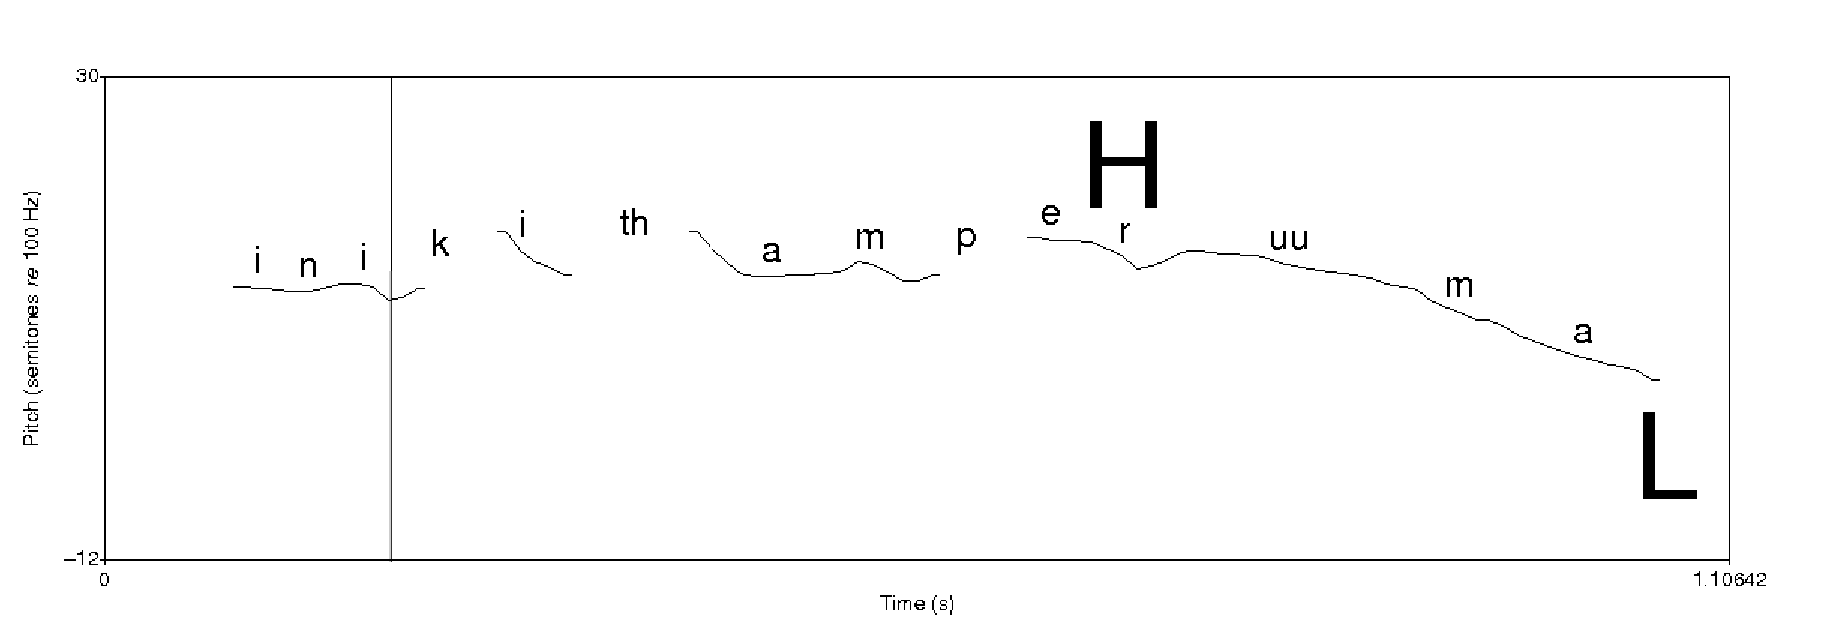
\includegraphics[width=0.5\textwidth]{./pics/kithamperuuma.eps}
\glll    ~   ~         H~~~~L\\
	 ini kitham-pe ruuma \\
     \textsc{prox} \textsc{1pl=poss} house  \\
    `This is our house.'
\z
} \\

In \xref{ex:phon:int:ass:kithamperuuma}, there is no presupposition, only a deictic reference (whose contour we will ignore for now) and an assertion \trs{kithampe ruuma}{our house}. The  assertion receives the HL contour, where H is linked to the beginning of the last lexical word \trs{ruuma}{house}\footnote{The pitch peaks after the k and the th are caused by aspiration and thus artefacts and not part of the intonation proper.} and the L is linked to the end of the utterance.

In \xref{ex:phon:int:ass:kithampenigirisujjadi}, we have a verbal predicate \trs{kitham=pe nigiri su-jaadi}{became our country}. The assertive contour is applied to the predicate with the high tone on the prefix of the last lexical word, the  verb. Then follows a drop to the end of the utterance. The constituents \trs{kaarang}{now}{} and \trs{ini}{\textsc{prox}}{} receive a presuppositive contour, discussed further below.

\xbox{14}{
\ea \label{ex:phon:int:ass:kithampenigirisujjadi}
 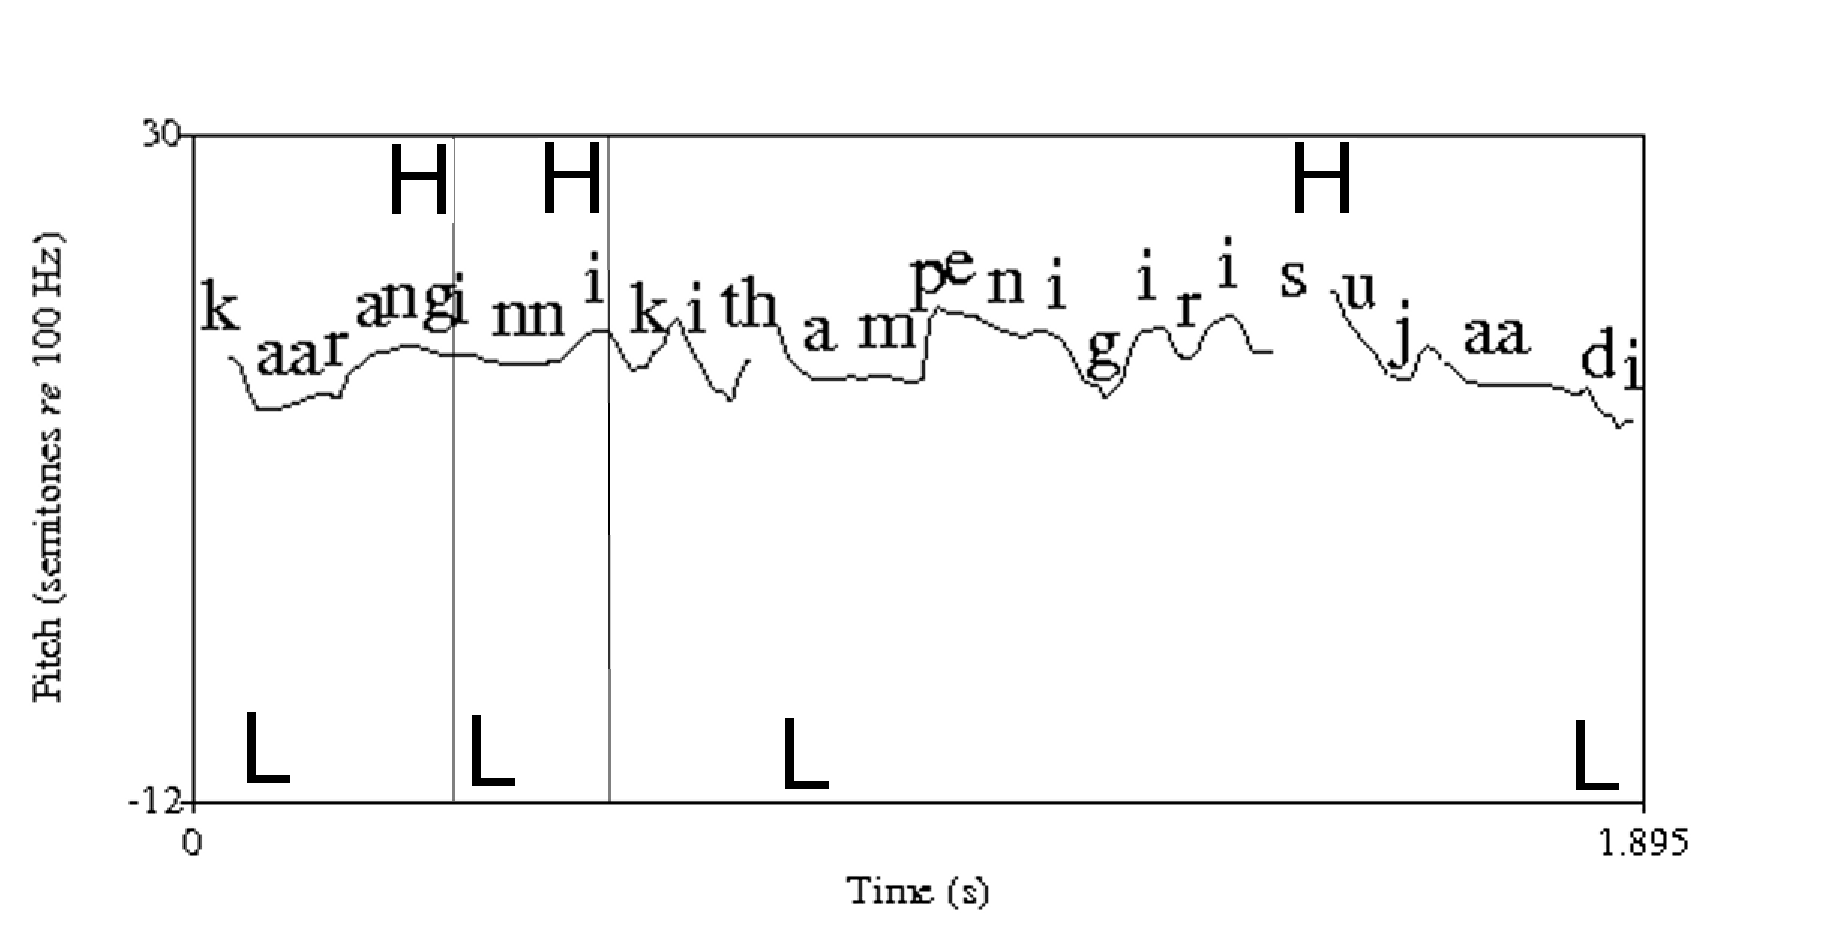
\includegraphics[width=0.5\textwidth]{./pics/newkithampenigiri.eps}
\glll    ~L   	H       ~L         H      ~      ~     H          L\\
	 kaarang $\mid$ inni  $\mid$ kitham=pe nigiri su-jaadi $\mid$\\
     now ~ \textsc{prox} ~ 1\textsc{pl}=\textsc{poss} country \textsc{past}-become \\
    `Now this has become our country.'
\z
} \\

Above we have seen that the last lexical word (noun, verb) receives the high tone of the assertive contour.
In the event that the assertion only contains functional elements, the description formulated above cannot apply. In this case,  the high tone is linked to the last word nevertheless, even if it is not lexical. An example is \trs{kitham}{1pl} in \xref{ex:phon:int:ass:oorampadajo}.

\xbox{14}{
\ea \label{ex:phon:int:ass:oorampadajo}
 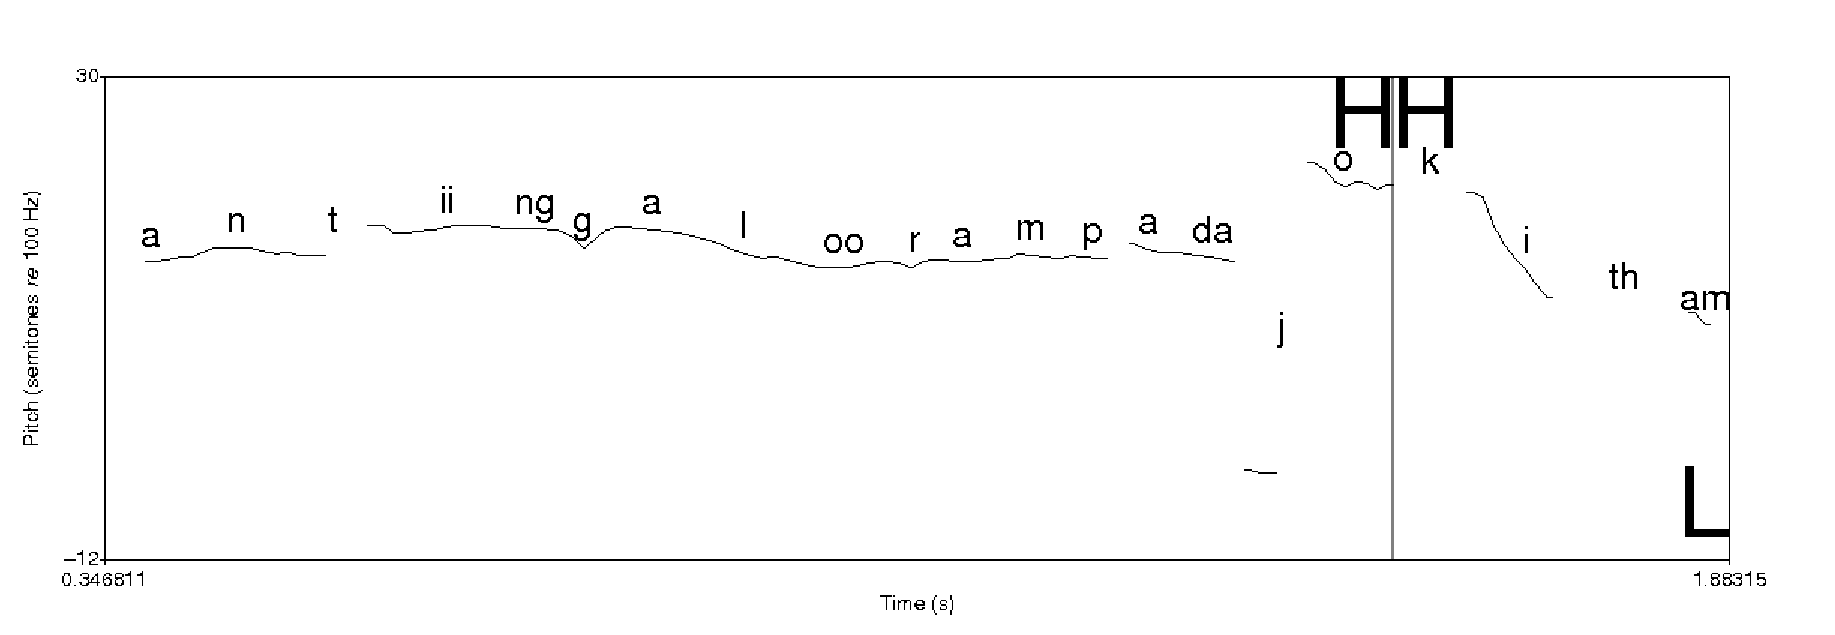
\includegraphics[width=0.5\textwidth]{./pics/oorampadajo.eps}
\glll ~      ~      ~       H       H      L\\
an-tiinggal ooram pada=jo $~\mid~$ kitham $~\mid$\\
 \textsc{past}-settle man \textsc{pl=foc} ~ \textsc{1pl} ~\\
`The people who settled down here are we.'
\z
} \\




In narrow focus, the high tone is linked to the element in focus even if this is not the last lexical element in the assertion. In \xref{ex:phon:int:ass:seelongoorangpada}, the speaker emphasizes the fact that the Malays are no longer East Asians, but Ceylonese. The two presuppositions \trs{kaarang}{now}{} and \trs{kithang}{we}{} are followed by the assertion \trs{SEELON ooram pada}{Ceylon people}. The presuppositions conform to the presuppositive contour, which will be discussed in more detail below. The assertion \em SEELON ooram pada \em receives the assertive HL contour, but H is linked to the emphasized element \em SEELON \em instead of the last lexical element \em ooram\em. This is marked in the graphic by a crossed out H where the normal tone would be expected.


\xbox{14}{
\ea \label{ex:phon:int:ass:seelongoorangpada}
 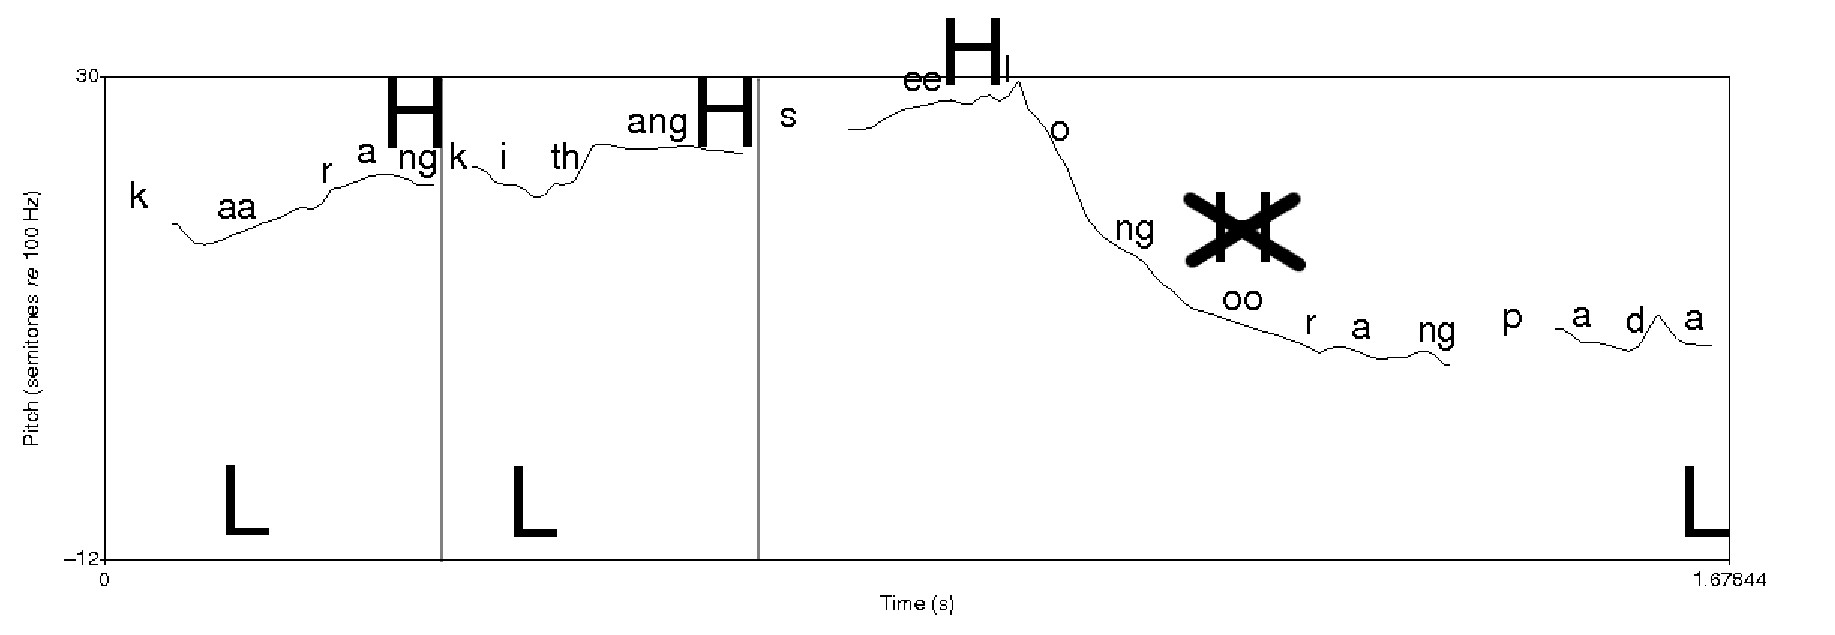
\includegraphics[width=0.5\textwidth]{./pics/seelongoorangpada.eps}
\glll ~~~L      H      ~~L       H      H        ~     ~   L \\
      kaarang $~\mid~$ kithang $~\mid~$ Seelong ooram pada $~\mid$ \\
     now { }   \textsc{1pl} { } Ceylon man \textsc{pl} { } \\
    `Now we are Ceylonese.'
\z
} \\

Imperatives also take the assertive contour, as the following example, taken from cooking instructions, shows. Note that the rice is presupposed and has been talked about earlier, which can be seen from the accusative marker \em =yang\em, which normally only attaches to inanimate referents when they are topical (see Section \ref{sec:morph:=yang}).


\xbox{14}{
\ea \label{ex:phon:int:ass:birrasyanthaaro}
 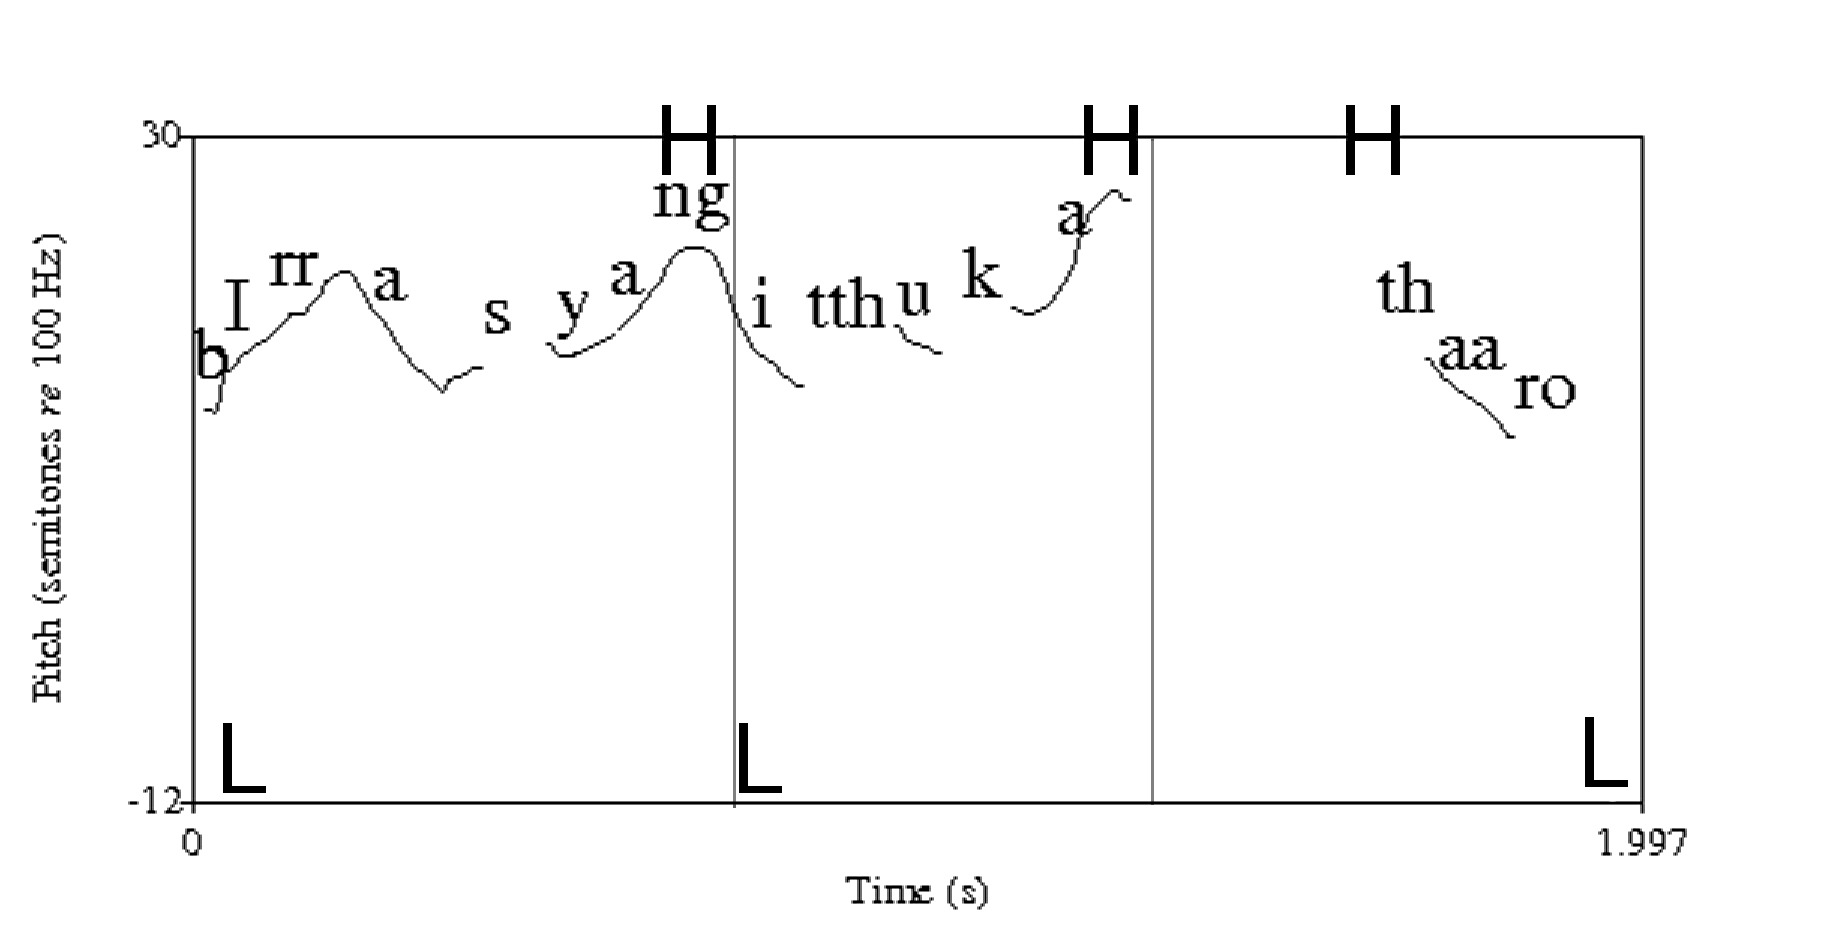
\includegraphics[width=0.5\textwidth]{./pics/birrasyangitthukathaaronew.eps}
\glll ~L             H    ~L       H       ~H       L \\
      bìrras=yang $~\mid$ itthu=ka $~\mid$  thaaro $~\mid$ \\
     raw.rice=\textsc{acc} { } \textsc{dem.dist}=\textsc{loc} { }  put { } \\
    `Add the rice to it!'
\z
} \\

\subsection{Progredient contour}\label{sec:phon:Progredientcontour}
The progredient contour is characterized by a slow steady rise to a high tone at the end. It is used for the non-final elements in a chain of assertions. The enumeration of ethnic groups in \xref{ex:phon:int:ass:cinggalaaada} shows slow rise from start to end of each of the first three phonological phrases, which are progredient. The last phonological phrase has the ``final'' contour, but the intensity decreases so that the graphic cannot represent the very low final pitch. The movement is clear when listening, though.


\xbox{14}{
\ea \label{ex:phon:int:ass:cinggalaaada}
 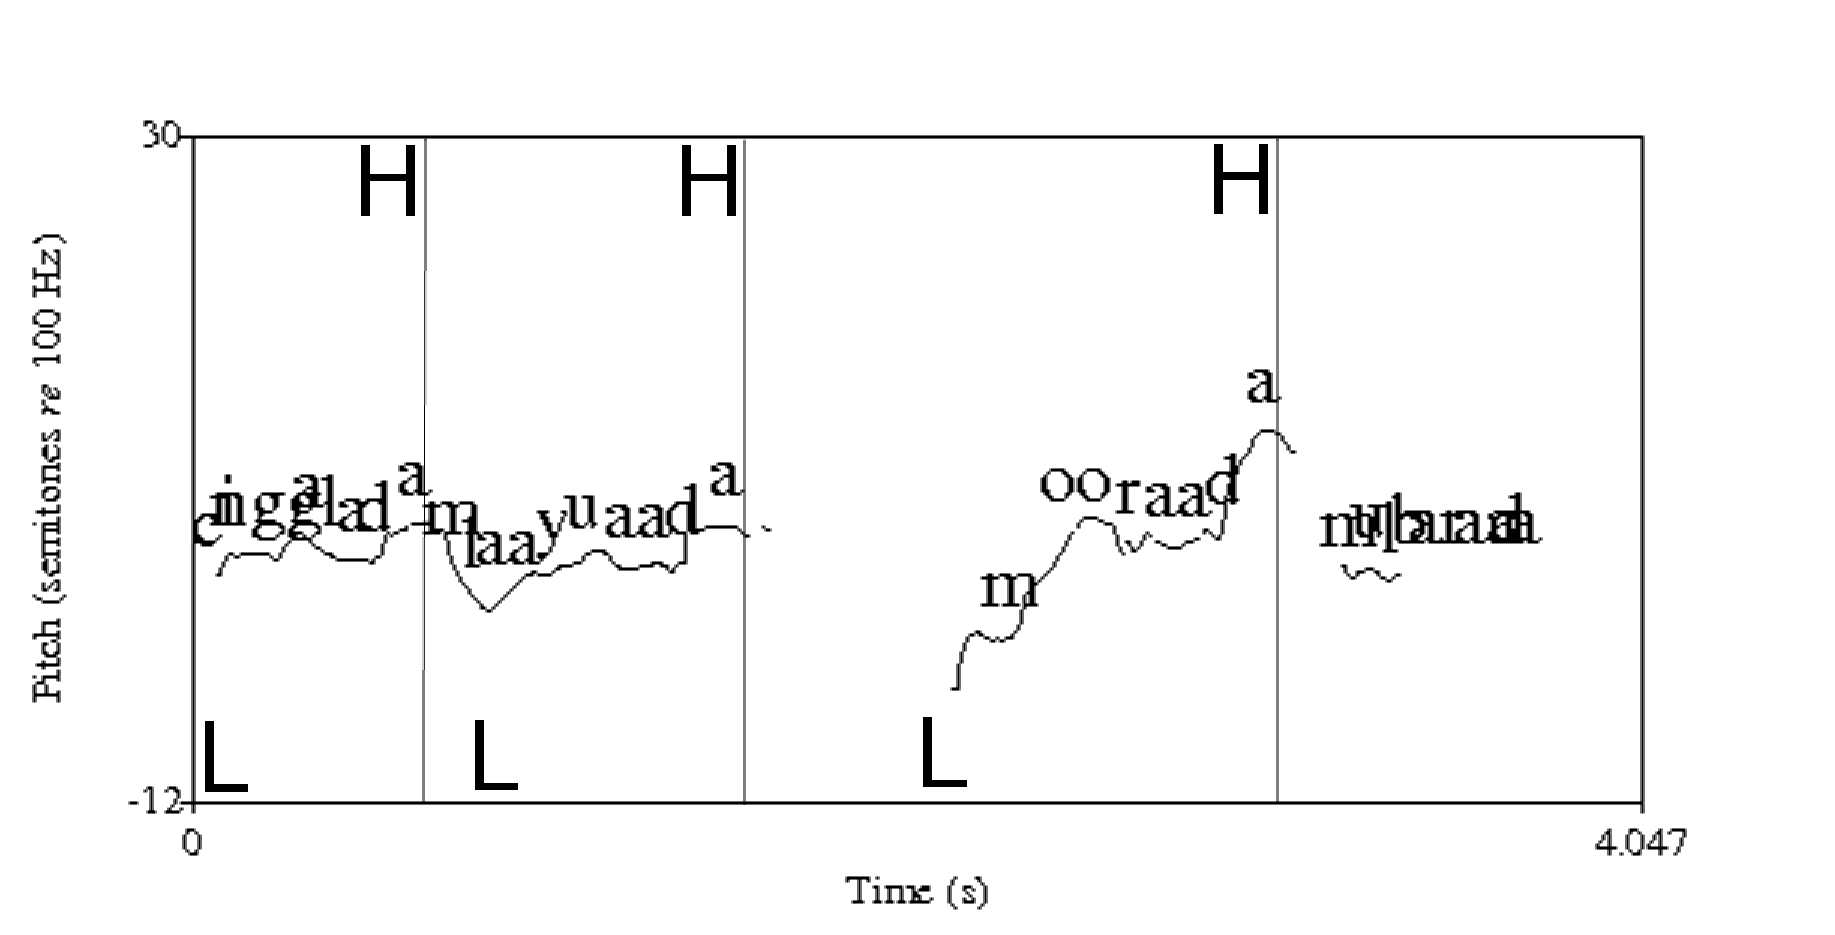
\includegraphics[width=0.5\textwidth]{./pics/cinggalaaadanew.eps}
\glll   L        ~ 	H  	L      ~ 	H  L    ~       H    ~        ~~ (L)\\
	cinggala aada $~\mid~$ 	mlaayu aada $~\mid~$ {\em moor} aada $~\mid~$ 	mùlbar aada $~\mid$\\
        Sinhala exist ~ Malay exist ~ Moor exist ~ Tamil exist ~\\
    `There are Sinhalese, there are Malays, there are Moors, there are Hindus.'
\z
} \\


\subsection{Presuppositive contour}\label{sec:phon:Presuppositivecontour}
The presuppositive contour is characterized by a steady fall to the last syllable and a following steep rise to a high tone target: LH. It is used for presupposed elements, which can be NPs, adjuncts or subordinate clauses.


Subordinate clauses always precede the main clause in SLM and are normally presupposed. Being presupposed, they are realized with a final H tone, normally preceded by a low tone. \xref{ex:phon:int:presup:braambath} illustrates this pattern. The high tone is on the right edge of \trs{kaaving}{marry}, while the low tone is immediately preceding. There is a second presupposition in this utterance \trs{ini mlaayu}{these Malays}. Just like the subordinate clause, this NP receives an LH contour. The assertion has a high tone on the past tense prefix \em su- \em of the last lexical word \trs{braambath}{spread}.


\xbox{18}{
\ea \label{ex:phon:int:presup:braambath}
 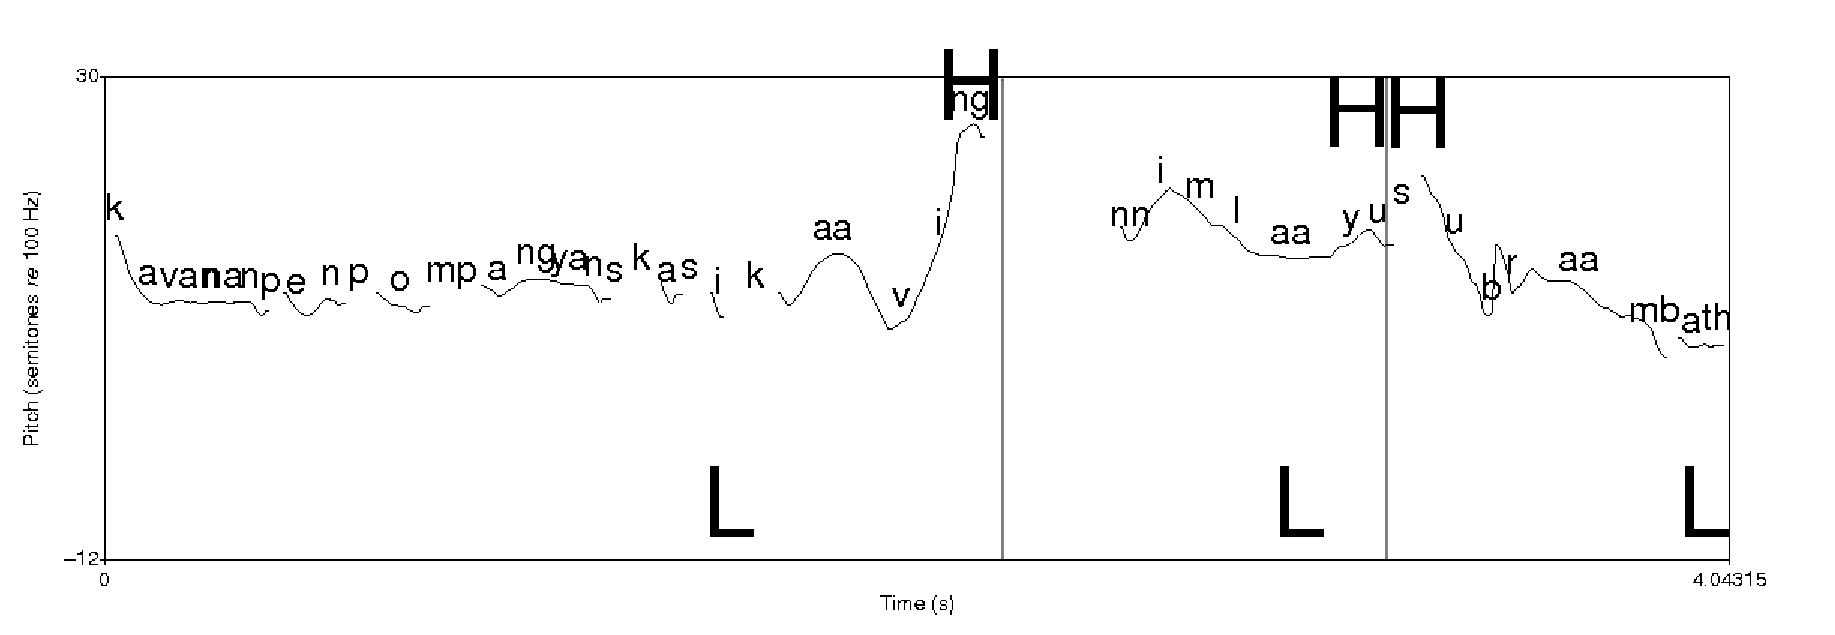
\includegraphics[width=0.5\textwidth]{./pics/braambath.eps}
\glll     ~    ~            ~         ~       ~~L     H          ~ ~~~L      H      H           L\\
	 ini kavanan=pe prompang=yang as-kasi kaaving $~\mid~$ nni mlaayu $~\mid~$ su-braa\u mbath $~\mid$\\
     \textsc{prox} group=\textsc{poss} female=\textsc{acc} \textsc{cp}-give marry ~ \textsc{prox} Malay ~ \textsc{past}-spread ~ \\
    `Having married their daughters, these Malays spread.' 
\z
} \\



In \xref{ex:phon:int:presup:blaajar}, there are two presupposed elements, and one assertion. The presupposed elements are \trs{kithampe aanak pada=jo}{our children}{} and \trs{skaarang}{now}. These receive a low tone on the nucleus of the last syllable (excluding the clitic \em =jo\em) and a high final tone. The assertion \trs{baenang cinggala sablaajar}{learnt Sinhala well}{} receives a high tone on the prefix of the last lexical word \trs{blaajar}{learn} and a low tone target assigned at the end.

\xbox{15}{
\ea \label{ex:phon:int:presup:blaajar}
 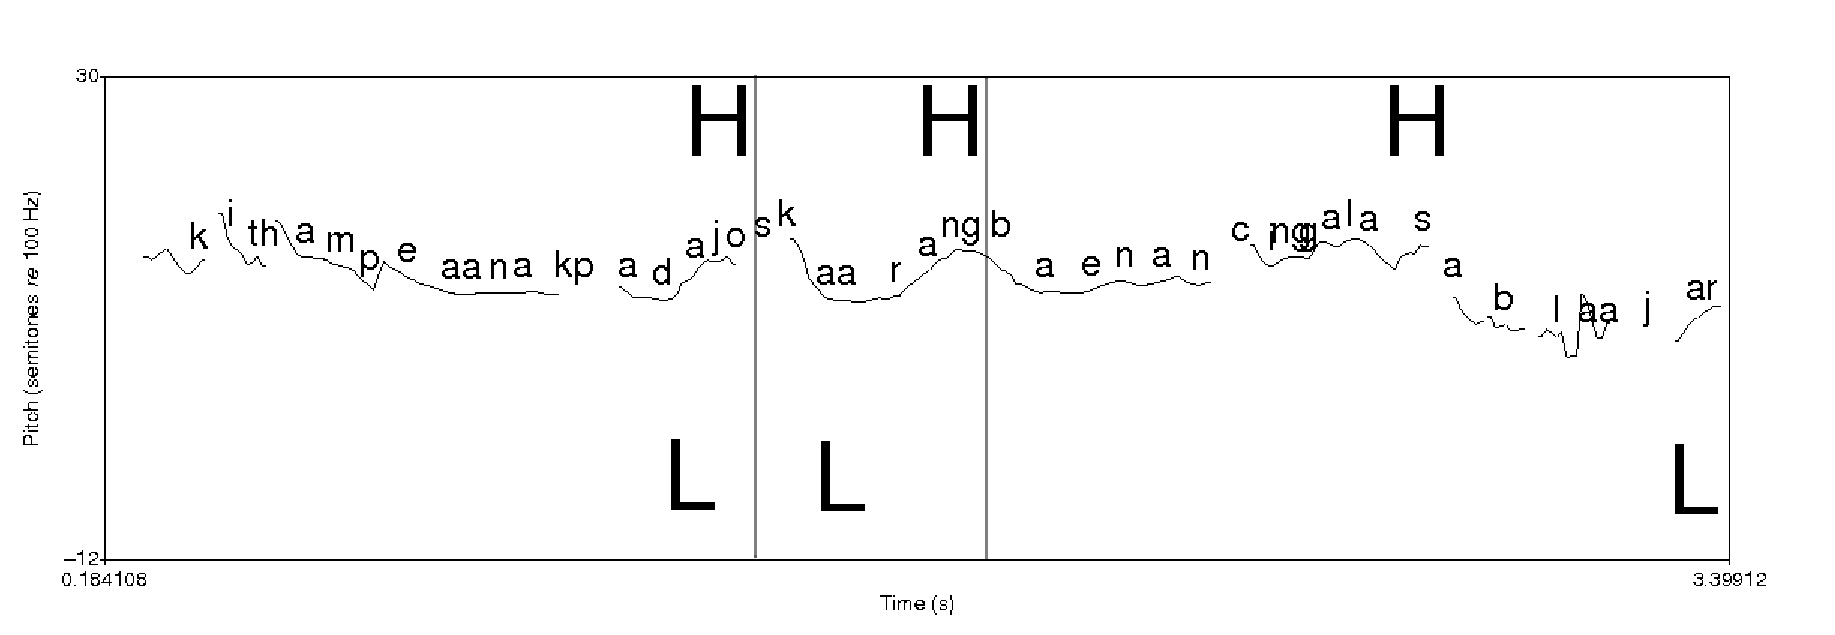
\includegraphics[width=0.5\textwidth]{./pics/blaajar.eps}
\glll ~      ~    ~~~~~L H  ~~~~L	 H  ~       ~       H L\\
 kitham=pe aanak pada=jo $~\mid~$ skaarang $~\mid~$ bae=na cinggala sa-blaajar $~\mid$\\
 \textsc{1pl=poss} child \textsc{pl}=\textsc{emph} ~ now ~ good=\textsc{dat} Sinhala \textsc{past}-learn ~\\
`Our children have learnt Sinhala well.'
\z
} \\

Things are similar in \xref{ex:phon:int:presup:laskallitherapi}, where the presupposed constituents \trs{laskalli}{again}{} and \trs{kithampe nigirinang}{to our country} receive a LH tone at the right edge. The assertion \trs{thàràpii}{did not go} receives high tone on the prefix of the last lexical element and a low final tone.

\xbox{14}{
\ea \label{ex:phon:int:presup:laskallitherapi}
 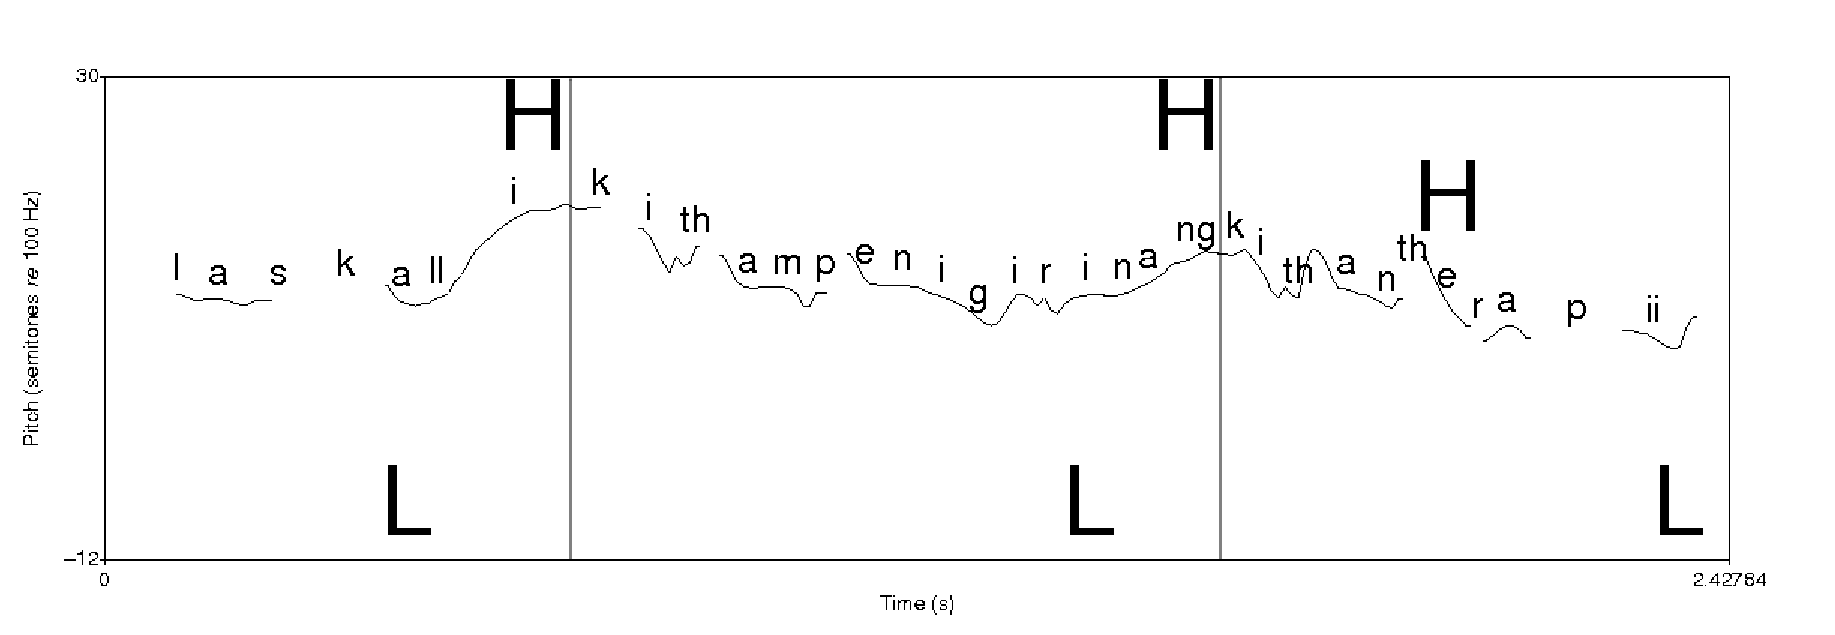
\includegraphics[width=0.5\textwidth]{./pics/laskallitherapi.eps}
\glll ~~~~L     H          ~     ~~~~~~L       H     ~      ~~~H        L  \\
      laskalli $~\mid~$  kitham=pe nigiri=nang $~\mid~$ kithang thàrà-pii $~\mid$ \\
      again ~ \textsc{1pl=poss} country=\textsc{dat} ~ \textsc{1pl} \textsc{neg.past}-go ~ \\
    `We did not go back to our country.' 
\z
} \\



\xref{ex:phon:int:presup:ciinggal} shows a more complex sentence. The presupposed constituent \trs{andaathang ooram pada}{the men who had come} receives a LH tone on the right edge. So do the subordinates \trs{spìrrang}{having waged war} and \trs{deranna asbanthu}{having helped him}. The predicate \trs{siinijo suciinggal}{settled down right here} receives a high tone on the  prefix of last lexical element \trs{ciinggal}{settle} and a low final tone.


\xbox{18}{
\ea \label{ex:phon:int:presup:ciinggal}
 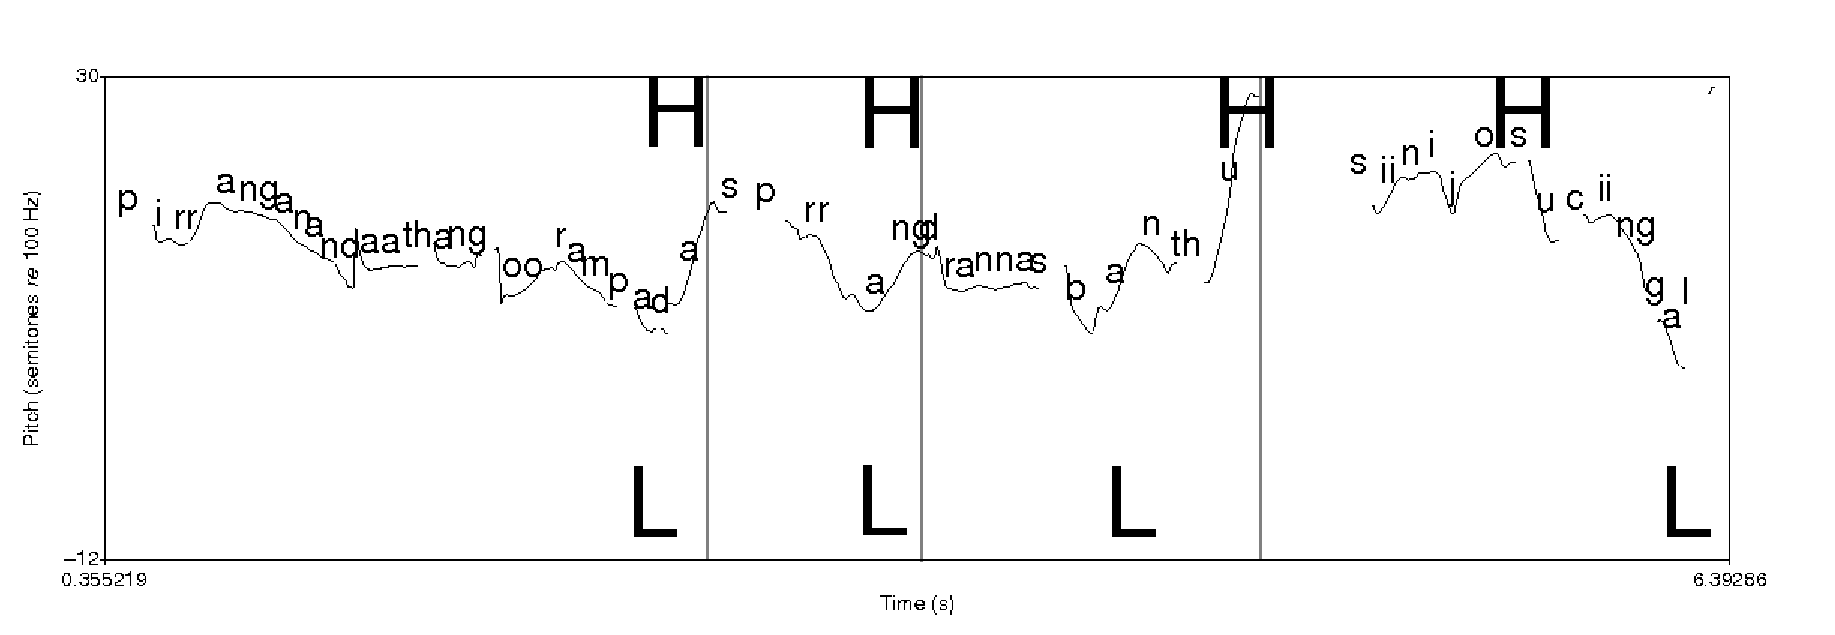
\includegraphics[width=0.5\textwidth]{./pics/ciinggal.eps}
\glll 	~ ~	~	~~L	H	~~~~~~~L	H	~	  ~~~~~~L 	H	~	H 		L\\
       pìirang=na an-daathang ooram pada $~\mid~$ s-pìrrang $~\mid~$  deran=na as-banthu $~\mid~$  siini=jo su-cii\u n\u ggal $~\mid$ \\
      war=\textsc{dat} \textsc{past}-come man \textsc{pl} ~ \textsc{cp}-wage.war ~ 3=\textsc{dat} \textsc{cp}-help ~ here=\textsc{emph} \textsc{past}-settle  \\
    `The men who had come, after having waged war and helped him, settled down.' 
\z
} \\

% The final example of this section shows layering of two contours in the first part, where we find a subordinate clause with a presuppositive contour, embedded in which there are again smaller presuppositive contours. The  pitch movement corresponds to the syntactic importance of the break. The first two movements are inside the subordinate clause and are less important, but the final movement is very steep.
% 
% \xbox{18}{
% \ea \label{ex:phon:int:presup:baaenanmgoornegnamblaakanginisanthangyangitthunamthuuvang}
%  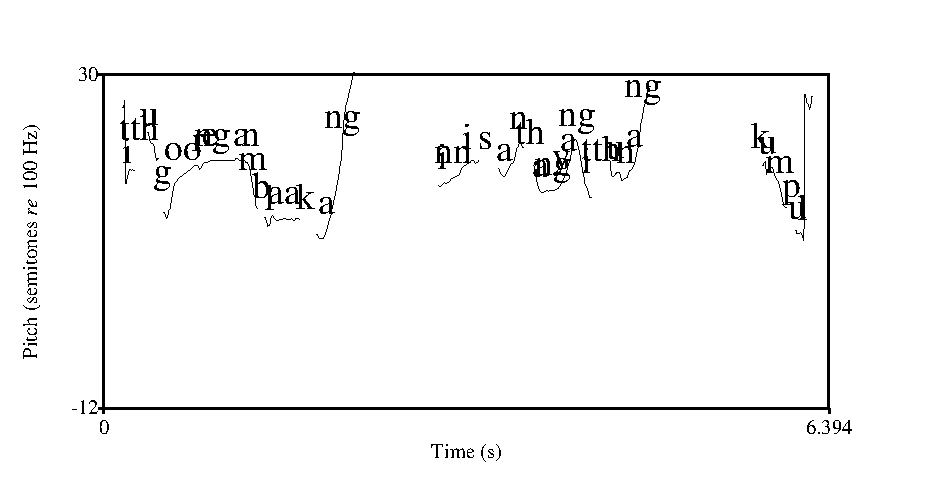
\includegraphics[width=0.8\textwidth]{./pics/itthugoorengnamblaakangnew.eps.eps}
% \glll L            H      L             H        L           H           ~~L        ~        H         L          H        H        L\\
%       itthu $~\mid~$  gooreng=nam $~\mid~$   blaakang $~\mid\mid~$   ini santhang=yang $~\mid~$   itthu=nam $~\mid~$   kumpul $~\mid~$  \\
%       good=\textsc{dat} ~ \textsc{inf}-fry=\textsc{dat} ~ after ~ \textsc{prox}    coconut.milk=\textsc{acc} ~  \textsc{dist=dat}  ~ pour\\
%     `After frying well, add the coconut milk to it.'
% \z
% } \\
% 




% see Stoel 2005


% Negative assertions have a similar contour \xref{ex:phon:int:ass:bissaratthukumpulan}. The pitch fall starts at the \em ku- \em of kumpulan.
% 
% \xbox{14}{
% \ea \label{ex:phon:int:ass:bissaratthukumpulan}
%  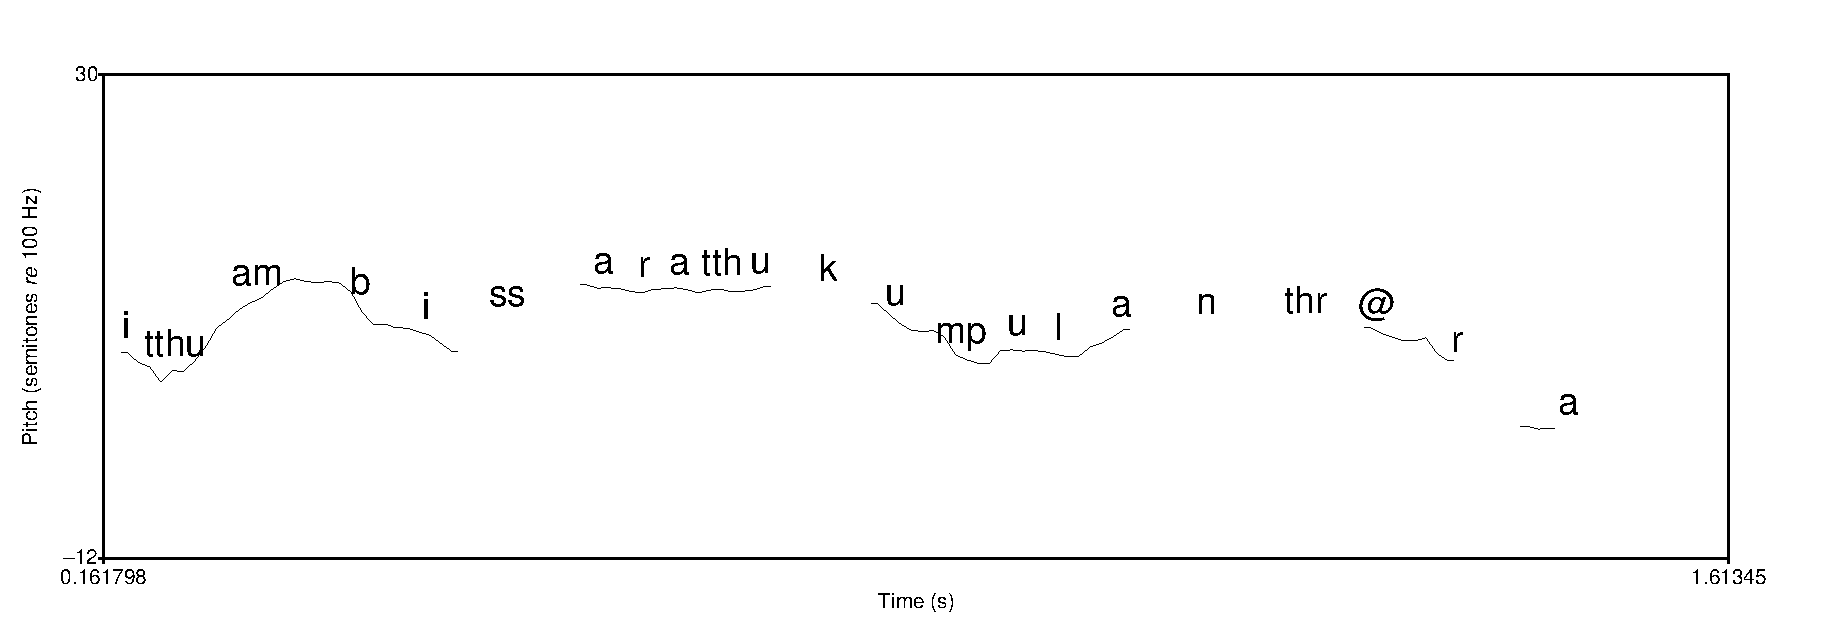
\includegraphics[width=0.5\textwidth]{./pics/neg.eps}
% \gll itthunam, bìssar atthu kumpulan th\E raa \\
%      therefore big \textsc{indef} association \textsc{neg}  \\
%     `Therefore, there are no big associations.'
% \z
% } \\



% \xbox{14}{
% \ea\label{ex:phon:int:ass:luppasthaangang}
%  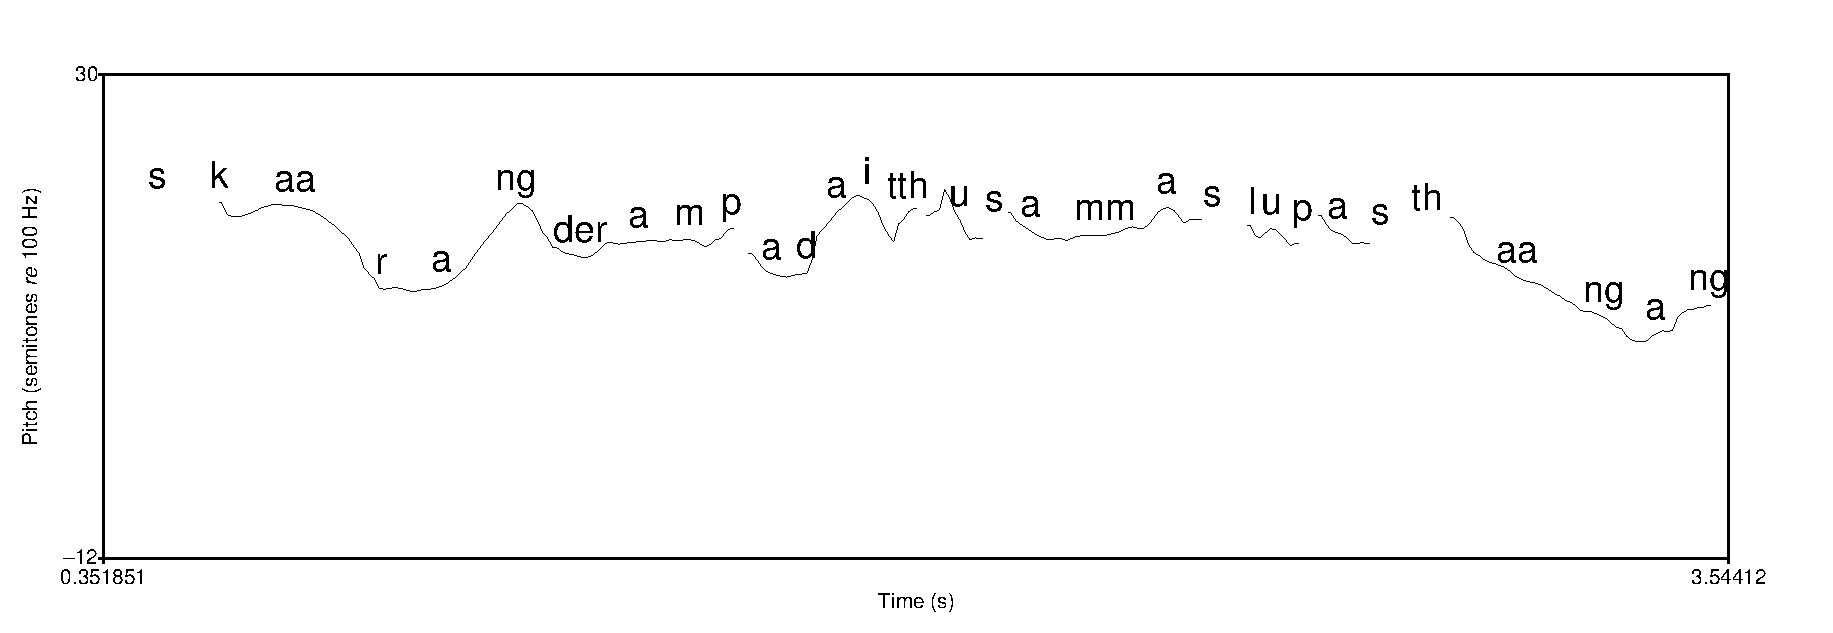
\includegraphics[width=0.5\textwidth]{./pics/luppasthaangang.eps}
% \gll skaarang dheram pada itthu samma as-luppas thaangang \\
%      now \textsc{3pl} \textsc{pl} \textsc{dist} all \textsc{cp}-leave hand  \\
%     `Now they left it all behind.'
% \z
% } \\






\subsection{Question contour}\label{sec:phon:Questioncontour}
The question contour is identical to the presuppositive contour: LH on the last syllable. It might be possible to combine them into a ``non-assertive'' contour; for expository reasons this is not done here. The question contour is used for interrogative illocution. Given that there is also segmental material which signals questions (WH-words or the clitic \em =si\em), the question contour is not obligatory if either of these are present.

Example  \xref{ex:phon:int:q:aapeyang} shows the question contour on a WH-question introduced by \trs{aapeyang}{what}. The pitch rises to the right edge from an immediately preceding low tone linked to \trs{kijja}{do}. The preceding NP \trs{dram pada}{they}{} and the preceding subordinate \trs{deram pada lae atthu pukuran mà-gijja thàrboole subbath}{Since they could not do other work}{} have the presuppositive contour, which is emically identical to the question contour. All three contours in this utterance have a final high  tone, and a preceding low tone, although the latter cannot be located exactly in the subordinate clause.


\xbox{12.5}{
\ea \label{ex:phon:int:q:aapeyang}
 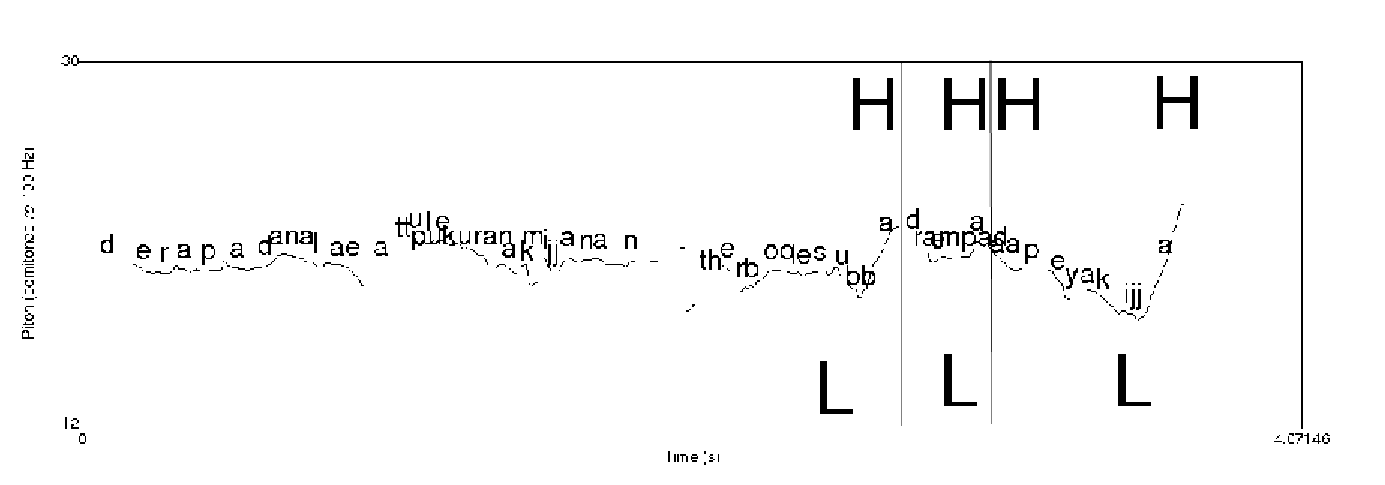
\includegraphics[width=0.5\textwidth]{./pics/aapeyang.eps}
\glll      ~    ~    ~    ~     ~      ~        ~        ~~L?         H      ~    ~~L   H       H         ~~~~~~L    H  \\
	 deram pada lae atthu pukuran mà-gijja thàrboole subbath $~\mid~$ dram pada $~\mid~$ aape=yang eng-kijja? $~\mid~$ \\
      \textsc{3pl} \textsc{pl} other \textsc{indef} work \textsc{inf}-make cannot because ~ \textsc{3pl} \textsc{pl} ~ what=\textsc{acc} \textsc{past}-do \\
    `Since they could not do other work, what did they do?' 
\z
} \\

YN-questions without the clitic \em =si \em also have the question contour, as in \xref{ex:phon:int:q:netherlandka}

\xbox{14}{
\ea \label{ex:phon:int:q:netherlandka}
 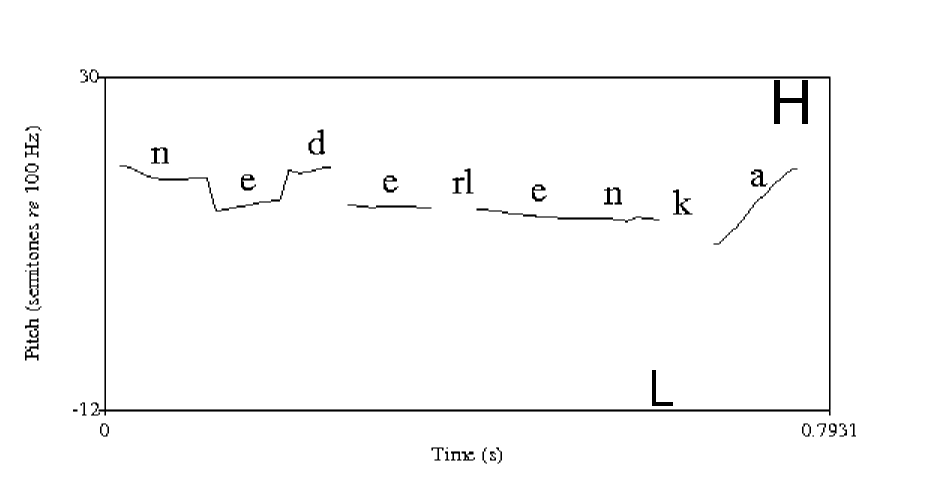
\includegraphics[width=0.5\textwidth]{./pics/nederlenkanewHL.eps}
\glll       ~  ~~~~~~~~~~~~~~~L       H \\
	{ } {\em Netherland}-ka $\mid$ \\
     {} Netherlands-\textsc{loc}  \\
    `Do they live in the Netherlands?' 
\z
}


Another example is \xref{ex:phon:int:q:gheena}, where the speakers ask a younger speaker for the word for `ghee'. The pitch rises steadily to the end of the question.


\xbox{14}{
\ea \label{ex:phon:int:q:gheena}
 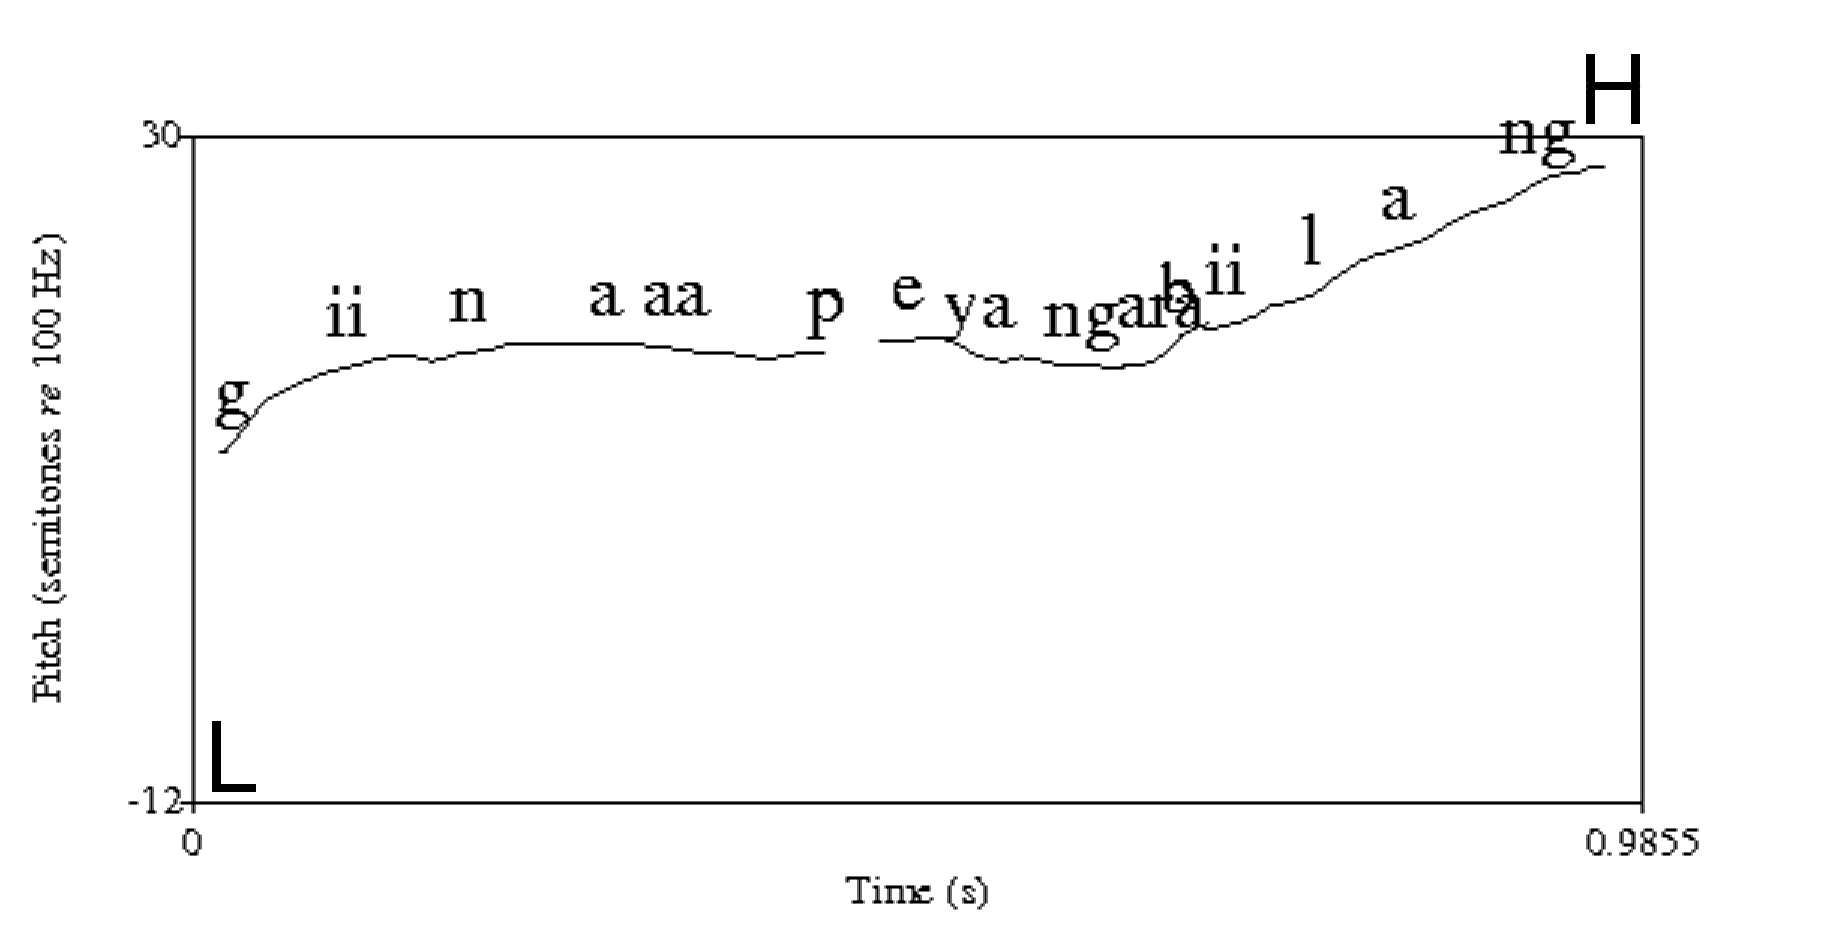
\includegraphics[width=0.5\textwidth]{./pics/gheenaaapeyangarabiilangnew.eps}
\glll       ~L  		~  ~     ~        H \\
	{\em ghee} =na aapeyang biilang $\mid$ \\
    { } =\textsc{dat} what say \\
    `How do you say for ``Ghee''?'
\z
}



When the interrogative clitic \em =si \em is present, the question contour can be present as in \xref{ex:phon:int:q:sudaarasudaari} or absent, as in \xref{ex:phon:int:q:puaasamuusing}. This seems to correlate with question type. In \xref{ex:phon:int:q:sudaarasudaari}, the speaker requests information about the existence of siblings, whereas in \xref{ex:phon:int:q:puaasamuusing} the speaker requests confirmation of her assumption that the addressee was not in Sri Lanka during the fasting period. Request for information is signalled both segmentally and suprasegmentally in \xref{ex:phon:int:q:sudaarasudaari}, while request for confirmation is only marked segmentally in \xref{ex:phon:int:q:puaasamuusing}, and not suprasegmentally.


\xbox{14}{
\ea \label{ex:phon:int:q:sudaarasudaari}
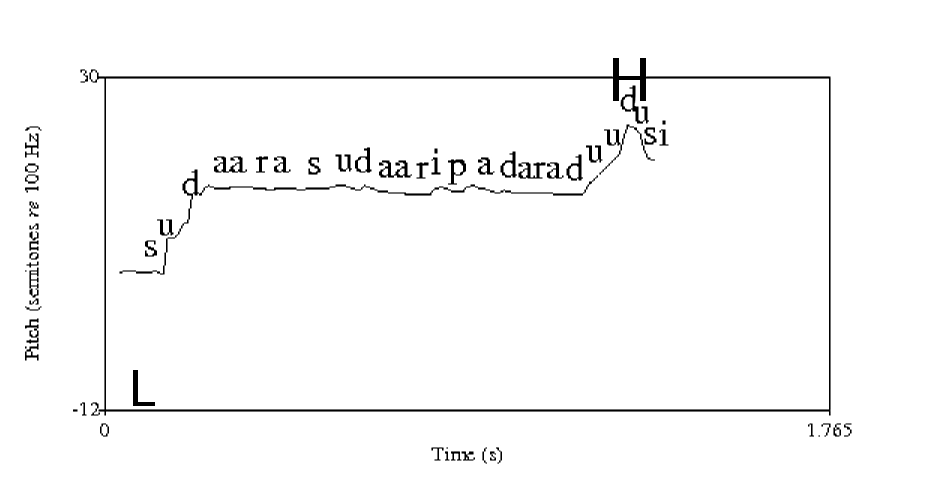
\includegraphics[width=0.5\textwidth]{./pics/sudaarasudaaripadanewHL.eps}
\glll ~L          ~        ~        ~~~~~~~~~~~~~H   \\
      sudaara sudaari pada arà-duuduk=si \\
      brothers sisters \textsc{pl} \textsc{non.past}-be=\textsc{interr}  \\
    `Do you have brothers or sisters?' 
\z
} \\


\xbox{14}{
\ea\label{ex:phon:int:q:puaasamuusing}
 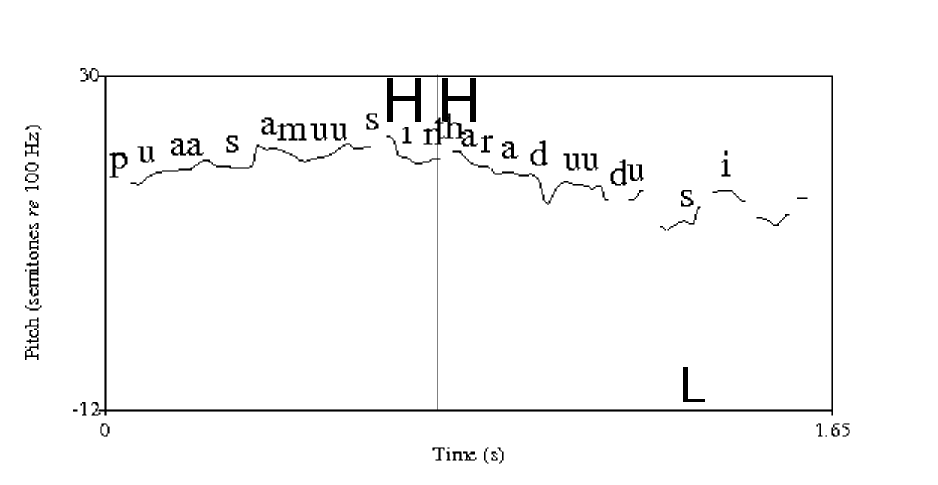
\includegraphics[width=0.5\textwidth]{./pics/puaasamuusing1newHL.eps}
\glll  ~      ~~~~~H	H~~~~~~~~~~~~L\\
       puaasa muusing thàrà-duuduk=si  \\
     fasting period \textsc{neg.past}-live=\textsc{interr}  \\
    `You were not here during the fasting period, were you?' 
\z
} \\


\subsection{Case study}\label{sec:phon:Casestudy}
The intonational patterns for assertions, questions and commands will be exemplified by a short conversation recorded in Badulla on  January 15, 2006. After some linguistic production stimulated by the researcher, the speakers have a little rest and chat about his family.  The existence of the recording device is forgotten. This fragment was chosen because of the naturalistic setting and because various concise speech acts with distinct intonation contours follow each other in short sequence.
Especially interesting are the different functions that interrogatives can have. They can be used to request information, or to request confirmation. This corresponds to different intonatory contours and to the presence or absence of the interrogative clitic \em =si.\em

%  B060115cvs03.trs


\begin{tabular}{lp{4cm}}\hspace{-1cm}
\xbox{12}{
\ea
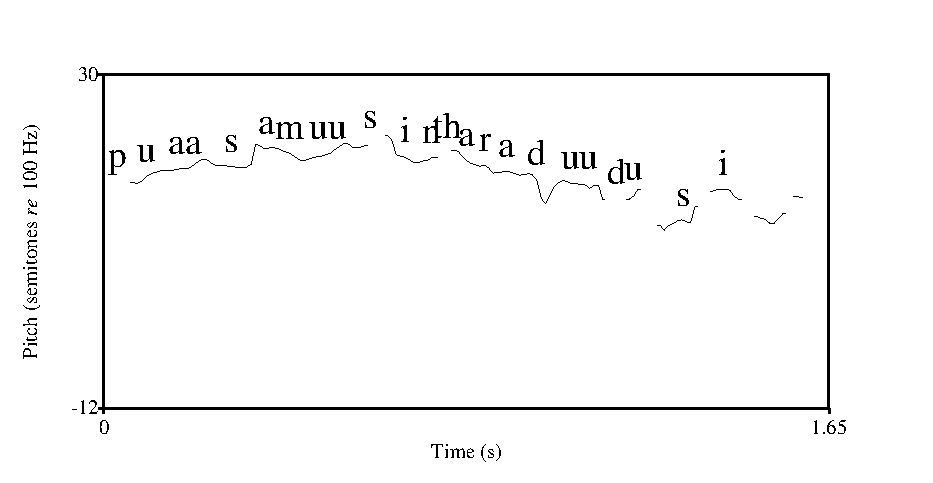
\includegraphics[width=0.5\textwidth]{./pics/puaasamuusing1new.eps}
\glll  ~     ~~~~H  ~ 		H 		L\\
     puaasa  muusing $\mid$ thàrà-duuduk=si $\mid$ \\
     fasting period ~ \textsc{neg.past}-live=\textsc{interr}  \\
    `You were not here during the fasting period, were you?' 
\z
} 
&\vspace{1cm}
 
 \textbf{Comment}: The negated predicate \trs{thàràduuduk}{were.not} together with \em =si \em indicate a presumption of absence, whose correctness is requested to be confirmed. The intonation contour is HL, like an assertion.\\
\end{tabular}


\begin{tabular}{lp{4cm}}\hspace{-1cm}
\xbox{12}{
\ea
 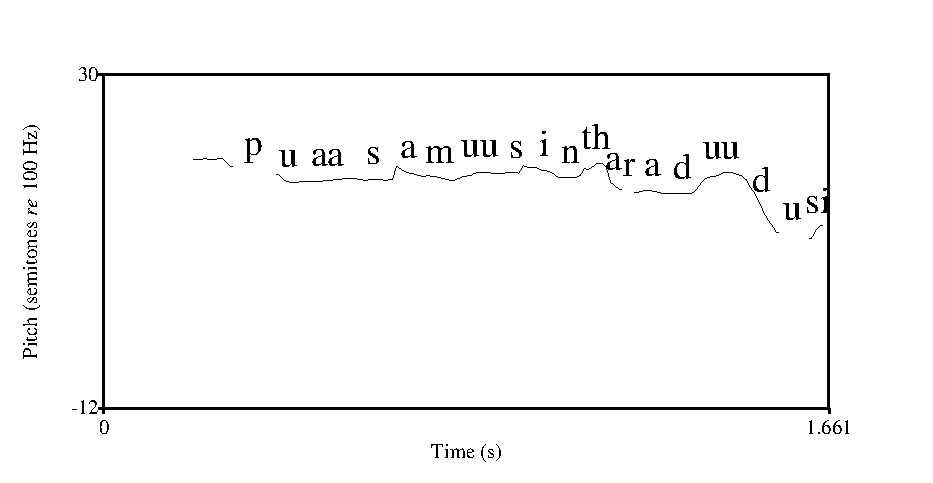
\includegraphics[width=0.5\textwidth]{./pics/puaasamuusing2new.eps}
\glll  ~     ~~~  ~ ~~~~~~~~~~H 		L\\
     puaasa muusing $\mid$ thàrà-duuduk=si $\mid$  \\
     fasting period ~ \textsc{neg.past}-live=\textsc{interr}  \\
    `You were not here during the fasting period, were you?'
\z
}
&\vspace{1cm}
 
 \textbf{Comment}: as above\\
\end{tabular}


\begin{tabular}{lp{4cm}}\hspace{-1cm}
\xbox{12}{
\ea
 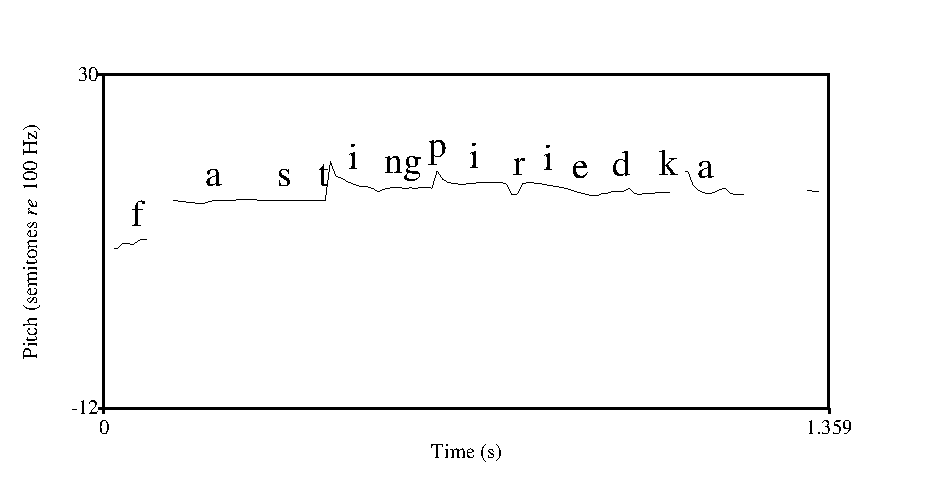
\includegraphics[width=0.5\textwidth]{./pics/fastingperiodkanew.eps}
\glll ~ ~ H\\
     {\em fasting} {\em period}=ka $\mid$ \\
     fasting period=\textsc{loc}  \\
    `In the fasting period' 
\z
}
&\vspace{1cm}
 
 \textbf{Comment}: an elaboration of the preceding question. Very slight rising intonation, since it is not a completely new question.\\
\end{tabular}



\begin{tabular}{lp{4cm}}\hspace{-1cm}
\xbox{12}{
\ea
 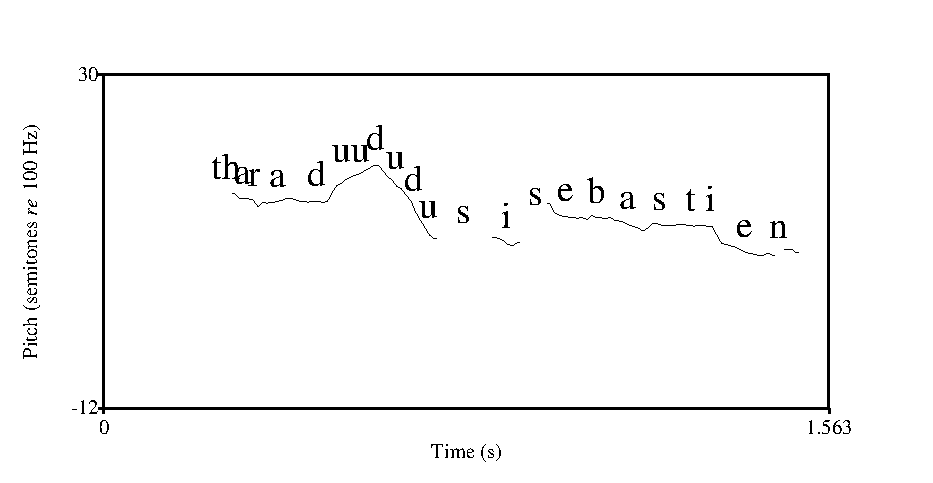
\includegraphics[width=0.5\textwidth]{./pics/tharaduudusisebastiennew.eps}
\glll ~~~~~~~~~~~H                   L ~ L\\
     thàrà-duudu=si $\mid$ Sebastian $\mid$  \\
     \textsc{neg.past}-stay=\textsc{interr} ~ Sebastian \\
    `You(=Sebastian) were not here, were you?'
\z
}
&\vspace{1cm}
 
 \textbf{Comment}: as above. The high tone of the assertional contour is linked to the beginning of the last lexical word, \trs{duuduk}{stay} in this case. The afterthought/anti-topic \citep{Chafe1976} \em Sebastian \em receives a new assertional intonation contour, but the pitch is not reset.\\
\end{tabular}



\begin{tabular}{lp{4cm}}\hspace{-1cm}
\xbox{12}{
\ea \label{ex:siithummabaapa}
 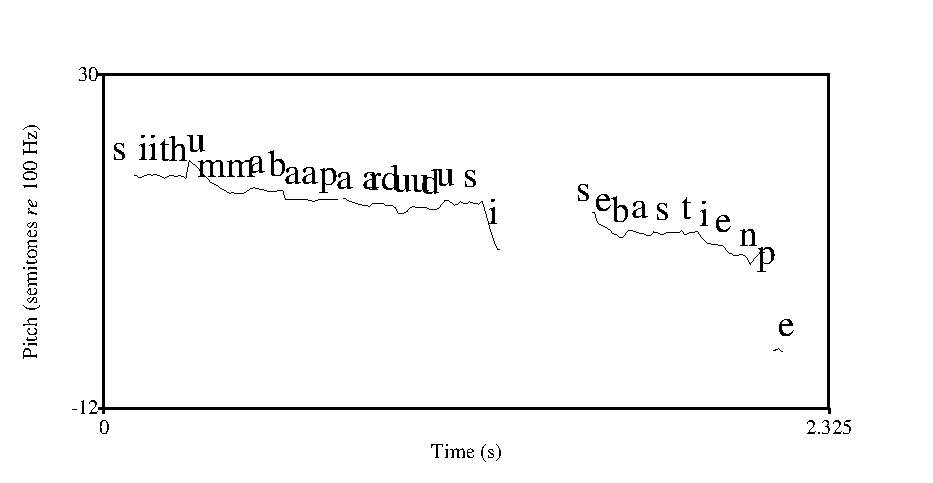
\includegraphics[width=0.5\textwidth]{./pics/siithummabaapaarduudusisebastianpenew.eps}
\glll ~       ~   ~          ~          L ~           L\\
    SLM1: siithu mma-baapa arà-duudu=si $\mid$ Sebastian=pe $\mid$ \\
    {} there mother-father \textsc{non.past}-stay=\textsc{interr} ~ Sebastian=\textsc{poss}   \\
    `Do your parents live there (i.e. Europe), Sebastian?' 
\z
}
&\vspace{1cm}
 
 \textbf{Comment}: In contrast to the preceding question, the afterthought \em Sebastian=pe \em is located in the same contour. The rather strong fall compared to the previous questions indicates security that my parents do indeed live there and reinforces the reading as a request for confirmation, rather than information.\\
\end{tabular}

\glossSTDmode
\begin{tabular}{lp{4cm}}\hspace{-1cm}
\xbox{12}{
\ea 
\gll SN: siithu?  \\
     {} there  \\
    `What do you mean by ``there''?' 
\z
} 
&\vspace{1cm}
 \textbf{Comment}: No intonation is given for the speech of the non-native variety spoken by the German researcher in order to avoid false conclusions drawn from this learner's phonology.\\
\end{tabular}

\glossINTmode
\begin{tabular}{lp{4cm}}\hspace{-1cm}
\xbox{12}{
\ea \label{ex:netherlandka}
 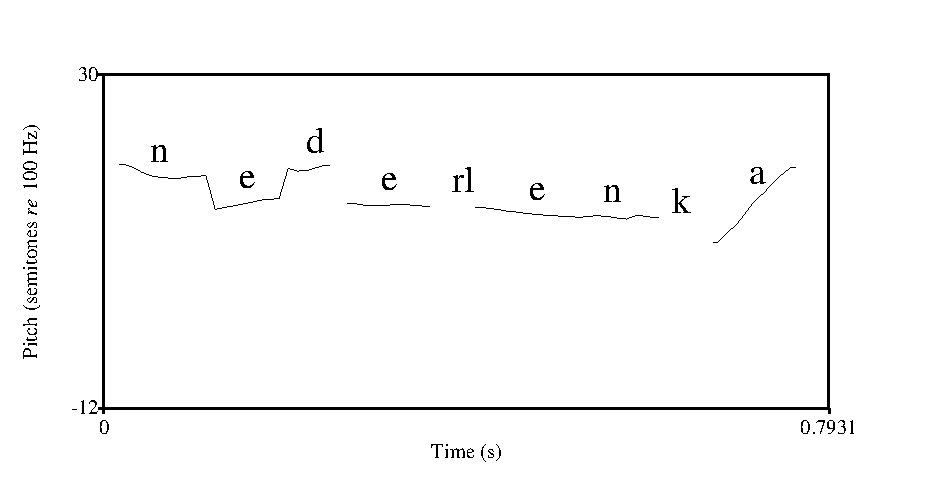
\includegraphics[width=0.5\textwidth]{./pics/nederlenkanew.eps}
\glll ~   ~~~~~~~~~~~~~~L H\\
     SLM1: {\em Netherland}=ka $\mid$?  \\
     {} Netherlands=\textsc{loc}  \\
    `Do they live in the Netherlands?' 
\z
}
&\vspace{1cm}
 \textbf{Comment}: Because the confirmation is declined, the question is restated, but with  a clear contour of request for information. \\
\end{tabular}

\glossSTDmode
\xbox{12}{
\ea 
\gll SN: {\em Germany}=ka.   \\
     {} Germany=\textsc{loc}  \\
    `They live in Germany.' 
\z
}\\

\glossINTmode
\begin{tabular}{lp{4cm}}\hspace{-1cm}
\xbox{12}{
\ea \label{ex:germanyka}
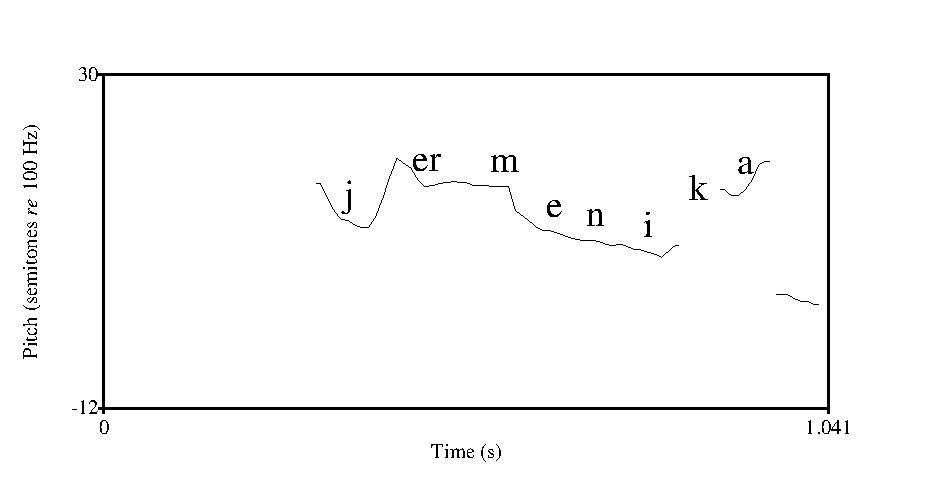
\includegraphics[width=0.5\textwidth]{./pics/jermenikanew.eps}
\glll ~    ~~H~~~~~~~~L H\\
     SLM1: {\em Germany}=ka $\mid$ \\
     {} Germany=\textsc{loc}  \\
    `Oh, so they live in Germany?' 
\z
}
&\vspace{1cm}
 
 \textbf{Comment}:Again a request for information, but less salient than the preceding one.  It indicates the surprise that members of my family live in separate countries, and requests confirmation of the veracity of that information. \em =si \em is not present.\\
\end{tabular}

\glossSTDmode
\xbox{12}{
 \ea 
\gll SN: {\em Germany}=ka.  \\
     {} Germany=\textsc{loc} \\
    `Yes, they live in Germany.' 
\z
}\\

\glossINTmode
\begin{tabular}{lp{4cm}}\hspace{-1cm}
\xbox{12}{
\ea \label{ex:sebastianaraduudukgermanyka}
\includegraphics[width=0.5\textwidth]{./pics/sebastianaraduudukjermannew.eps}
\glll ~  ~ ~ ~H L\\
      SLM1: Sebastian arà-duuduk {\em German} $\mid$.\\
     {} Sebastian \textsc{non.past}-stay Germany\\
    `So you live in Germany.'
\z
}
&\vspace{1cm}
 
 \textbf{Comment}: A tentative conclusion with a slight assertional contour. Listening to the example gives an impression of hesitation. The tentative conclusion seems to be `If the parents live in Germany, so must the son.'\\
\end{tabular}

\glossSTDmode
\xbox{12}{
\ea 
\gll   SN: no se se=jo {\em Netherlands}=ka,  se=ppe mma-baapa  {\em Germany}=ka   \\
       {} (no) \textsc{1s} \textsc{1s}=\textsc{emph} Netherlands=\textsc{loc}, \textsc{1s}=\textsc{poss} mother-father Germany=\textsc{loc} \\
    `No, \underline{I} live in the Netherlands, my parents live in Germany.'
\z
}\\

\glossINTmode
\begin{tabular}{lp{4cm}}\hspace{-1cm}
\xbox{12}{
\ea \label{ex:deranggermanyka}
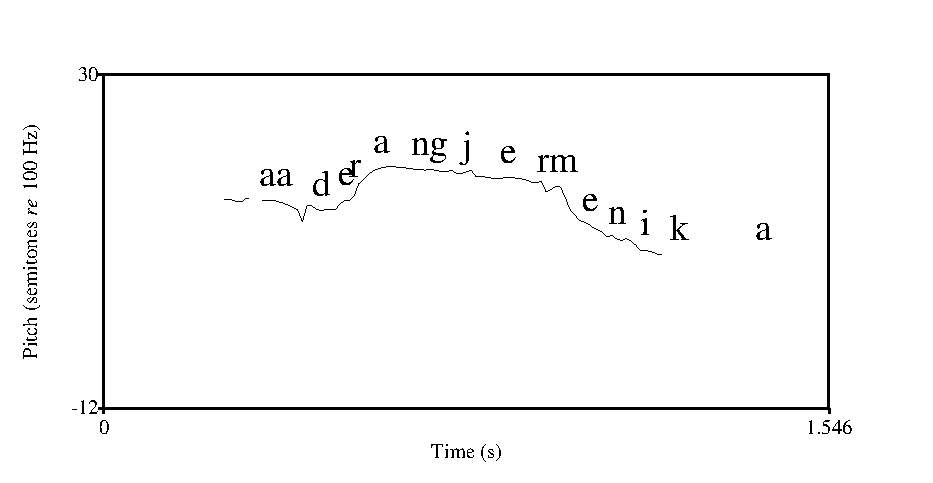
\includegraphics[width=0.5\textwidth]{./pics/aaderangjemernikanew.eps}
\glll  ~ ~~~~~~~H ~~H L\\
      SLM1: derang {\em Germany}=ka $\mid$ \\
     {} 3p Germany=\textsc{loc}.  \\
    `So they are in Germany.' 
\z
}
&\vspace{1cm}
 
 \textbf{Comment}: The solution of the mystery of parents and son living in different countries receives an assertional contour.\\
\end{tabular}

\begin{tabular}{lp{4cm}}\hspace{-1cm}
\xbox{12}{
\ea \label{ex:sudaarasudaari}
\includegraphics[width=0.5\textwidth]{./pics/sudaarasudaaripadanew.eps}
\glll ~          ~          ~     ~ ~             H\\
     SLM4: sudaara sudaari pada arà-duuduk=si $\mid$ \\
     {} brothers sisters \textsc{pl} \textsc{non.past}-be=\textsc{interr}  \\
    `Do you have brothers or sisters?'
\z
}
&\vspace{1cm}
 \textbf{Comment}: A new topic: siblings. The contour is a request for information with a rising pitch since there are no presumptions  available.\\
\end{tabular}

\glossSTDmode
\xbox{12}{
\ea 
\gll SN: {\em Germany}=ka duuva aade prompang aada  \\
     {} Germany=\textsc{loc} two younger.sibling woman exist  \\
    `I have two younger sisters who live in Germany' 
\z
}\\

\glossINTmode
\begin{tabular}{lp{4cm}}\hspace{-1cm}
\xbox{12}{
\ea 
\includegraphics[width=0.5\textwidth]{./pics/nexttimeaajibanew.eps}
\glll ~       ~  ~    ~   H       ~~~H~~L  H     ~        ~ ~ H\\
     SLM5: thraa. next time $\mid$ aajibaa-la $\mid$ kithan=na suuka mà-liiyath-na $\mid$\\
     {} no next time ~  bring-\textsc{imp} ~ \textsc{1pl}=\textsc{dat} like \textsc{inf}-see-\textsc{dat}  \\
    `So bring them next time, we would like to see them (won't you)' 
\z
} 
&\vspace{1cm}
 \textbf{Comment}: This contour is difficult to interpret from pitch movement alone, but auditory impressions make it clear that we are dealing with a command. The rising pitch at the end might indicate mitigation, but this is unclear as of yet.\\
\end{tabular}

\begin{tabular}{lp{4cm}}\hspace{-1cm}
\xbox{12}{
\ea \label{ex:fotopadathraa}
\includegraphics[width=0.5\textwidth]{./pics/fotopadathraanew.eps}
\glll   ~  ~~~H    ~    ~ L\\
       SLM2: {\em photo} pada thraa $\mid$ \\
     {} photo \textsc{pl}  \textsc{neg}.exist\\
    `You have no photos?' 
\z
}
&\vspace{1cm}
 
 \textbf{Comment}: Again a new topic, but with the underlying assumption that I have indeed not brought any photos: assertional contour. Note the absence of the clitic \em =si \em despite the question illocution.\\
\end{tabular}

\glossSTDmode
\begin{tabular}{lp{4cm}}\hspace{-1cm}
\xbox{12}{
\ea \label{ex:fotopadathraasi}
\gll SLM1: {\em photo} pada thraa=si \\
     {} photo \textsc{pl}  \textsc{neg}.exist=\textsc{interr}\\
    `You have no photos, have you?' 
\z
}
&\vspace{1cm}
\textbf{Comment}: No analysis due to problems with the sound file. (Multiple speakers at the same time, background noise)\\
\end{tabular}

\begin{tabular}{lp{4cm}}\hspace{-1cm}
\xbox{12}{
\ea 
\gll SLM6: gaa\u mbar gaa\u mbar. \\
     {} ``gaa\u mbar'' ``gaa\u mbar''.  \\
    `The word is ``gaa\u mbar''.
\z
}
&\vspace{1cm}

\textbf{Comment}: No analysis due to problems with the sound file\\
\end{tabular}

\begin{tabular}{lp{4cm}}\hspace{-1cm}
\xbox{12}{
\ea 
\gll  SLM1: thraa, thraa\\
      {} \textsc{neg}.exist, \textsc{neg}.exist\\
    `No, he has no photos.' 
\z
}
&\vspace{1cm}

\textbf{Comment}: No analysis due to problems with the sound file\\
\end{tabular}

\begin{tabular}{lp{4cm}}\hspace{-1cm}
\xbox{12}{
\ea \label{ex:sebastianskaaving}
\gll SLM3: Sebastian s-kaaving?   \\
     {} Sebastian \textsc{cp}-marry  \\
    `Is Sebastian married.' (asking other women)
\z
}
&\vspace{1cm}

\textbf{Comment}: No analysis due to problems with the sound file\\
\end{tabular}

\glossINTmode
\begin{tabular}{lp{4cm}}\hspace{-1cm}
\xbox{12}{
\ea \label{ex:sebastianthamakaavingsi}
\includegraphics[width=0.5\textwidth]{./pics/sebastianthamakaavingnew.eps}
\glll ~       ~  ~       L     ~          H     H              L\\
     SLM1: thàra thàra $\mid$ Sebastian $\mid$ thama-kaaving=si $\mid$  \\
     {} no no ~ Sebastian ~ \textsc{neg.nonpast}-marry=\textsc{interr}  \\
    `You are not married, are you?' 
\z
}
&\vspace{1cm}
 
 \textbf{Comment}:The presupposition is that I am not married. The overall contour is assertional, a request for confirmation. The very slight rise at the end indicates a remainder of doubt (cf. \xref{ex:fotopadathraa}).\\
\end{tabular}


\begin{tabular}{lp{4cm}}\hspace{-1cm}
\xbox{12}{
 \ea \label{ex:srilankakajokaaving}
\includegraphics[width=0.5\textwidth]{./pics/srilankakajokaavingnew.eps}
\glll ~      ~   ~          H ~     L\\
     SLM1: Sri Lanka=ka=jo $\mid$ kaving  $\mid$ \\
     {} Sri Lanka=\textsc{loc}=\textsc{emph} ~ marry  \\
    `Marry in Sri Lanka!' 
\z
}
&\vspace{1cm}
 
 \textbf{Comment}:A jocular imperative. The high tone is located at the end of the argument phrase/the beginning of the predicate phrase (The plateau around the second k is an artefact.)\\
\end{tabular}

\glossSTDmode

% Short and long vowels can be distinguished phonetically in SLM. Long vowels can only be found in the penultimate syllable of disyllables and of trisyllables with a schwa in the first syllable. \citet{Bichsel} and \citet{SmithEtAl2004} argue that vowel length is phonemic, while \citet{Tapovanaye1995} argues that it is a function of syllable structure. The vowel is used to contribute an extra mora required by word structure. In Section \ref{sec:phon:wordstructure} we will show that vowel length can indeed be predicted on the basis of word structure and is thus not phonemic.
\setcounter{exx}{0}\setcounter{footnote}{0}
     	\chapter{Major and minor word classes}\label{sec:form:freemorphemes}
\glossSTDmode
This chapter gives an overview over SLM free morphemes.  The chapter thereafter will treat bound morphology. Free morphemes comprise both lexical and functional morphemes. These fall into a number of classes, which will be discussed in turn.

Four major word classes are distinguished in SLM:
verbs like \trs{maakan}{eat} \formref{sec:wc:Verbs},
nouns like \trs{aanak}{child} \formref{sec:wc:Nouns},
adjectives like \trs{kiccil}{small} \formref{sec:wc:Adjectives},
and adverbs like \trs{kumaareng}{yesterday} \formref{sec:wc:Adverbs}. These classes are all fairly large and can accept new members. The members of a class all share certain characteristics, by which class membership can be checked.

There are also a number of minor classes such as personal pronouns, which are rather small and which cannot accept new members. Of these classes, a full extensional list of members will be given, along with some characteristic traits.

\section{Verbs}\label{sec:wc:Verbs}
SLM Verbs can be subdivided into canonical verbs, which are the largest subclass \formref{sec:wc:Canonicalverbs}, two existentials \formref{sec:wc:Existentialverbs:intro}, and a number of defective verbs, which cannot take the whole array of morphology available for canonical verbs \formref{sec:wc:Defectiveverbs}. Verbs can combine with other verbs in multi-verb constructions, of which an overview is given in Section \formref{sec:wc:Multi-verbconstructions}.  Some canonical verbs have also acquired a grammatical meaning when combined with other verbs. These are the vector verbs, which will be discussed in Section \formref{sec:wc:Vectorverbs}. Finally, verbs can participate in a number of special constructions, like the perfect construction, which will be discussed in Section \formref{sec:wc:Specialconstructionsinvolvingverbalpredicates}.

\subsection{Canonical verbs}\label{sec:wc:Canonicalverbs}
Sri Lanka Malay has a large class of verbs, which most often denote events like \trs{laari}{run}, but  states like \trs{thiidor}{sleep} can also be found in this class. All verbs share the following characteristics:

\begin{enumerate}
\item They can take the following affixes:
	non-past tense \em arà-\em,
	past tense \em anà-\em,
	past tense \em su-\em,
	anterior tense \em asà-\em,
	irrealis \em anthi-\em,
	infinitive \em mà-\em, as well as some additional minor TAM-affixes.
\item They are negated by preposed \em thàrà- \em for past tense, postposed \em thraa \em for perfect,  preposed \em thama- \em for present and future and \em jamà- \em for nonfinite contexts.
\item They are never negated by \em bukang\em.
\item They must be reduplicated in order to modify other predications
\end{enumerate}

There is a risk to mistake adjectives for verbs because adjectives can easily convert to verbs and take verbal morphology. Therefore, test for adjectivehood should also be done for candidate verbs to exclude this. See further discussion in the section on adjectives \formref{sec:wc:Adjectives}. An example of a verb would be \trs{laari}{run}, which could be inflected as \trs{aràlaari, anàlaari, anthilaari, {\em etc.}}{run, ran, will run, etc.}. This verb would be negated as \em thàràlaari \em for past tense, as \em thamalaari \em for non-past tense, and as \em laari thraa \em in the perfect. \em Laari  \em can never be negated by \em bukang\em, and would have to be used as \em laari\~{}laari \em in order to modify another predication.



\subsection{Existential verbs}\label{sec:wc:Existentialverbs:intro}
There are two existentials,  \em aada \em \formref{sec:wc:Existentialverbs:aada} and \em duuduk \em \formref{sec:wc:Existentialverbs:duuduk}. The latter can only be used with animate referents, while the former  can be used with both animate and inanimate referents. \em Duuduk \em thus carries a positive specification for animacy, while \em aada \em is underspecified for animacy.

Example \xref{ex:Kluumbukaruuma} shows that the animate existential \em duuduk \em cannot combine with the inanimate referent \trs{ruuma}{house}. Here, \em aada \em has to be used. Example \xref{ex:Kluumbukamlaayu} shows that both \em aada \em and \em duuduk \em can combine with the animate referent \trs{mlaayu pada}{Malays}.

\xbox{16}{
\ea \label{ex:Kluumbukaruuma}
\gll Kluu\u mbu=ka ruuma pada \textbf{aada}/*arà-duuduk. \\
     Colombo=\textsc{loc} house \textsc{pl} exist/\textsc{non.past}-exist.\textsc{anim}. \\
    `There are houses in Colombo.' (K081103eli02)
\z
}


\xbox{16}{
\ea\label{ex:Kluumbukamlaayu}
\gll Kluu\u mbu=ka mlaayu pada \textbf{aada/arà-duuduk}. \\
     Colombo=\textsc{loc} house \textsc{pl} exist/\textsc{non.past}-exist.\textsc{anim}. \\
    `There are Malays in Colombo.' (K081103eli02)
\z
}


% \xbox{16}{
% \ea\label{ex:form:aada:anim}
% \gll Appointed MPs             pada  \textbf{anà-duuduk}. \\
%       appointed MPs \textsc{pl} \textsc{past}-exist.\textsc{anim} \\
%     `There were appointed MPs.' (N061031nar01)
% \z
%. \\
% \xbox{16}{
% \ea
% \gll Bannyak Muslim oorang pada araduuduk. \\
%      many Muslim man \textsc{pl} \textsc{non.past}-exist.\textsc{anim}. \\
%     `There are many Muslims (in the Middle East.' (K061026prs01)
% \z
%. \\

\subsubsection{\em aada\em}\label{sec:wc:Existentialverbs:aada}
\em Aada \em is one of the most frequent morphemes in SLM. It is normally pronounced \phonet{aa\dz a} and rarely \phonet{aa\textsubplus{\:r}a}. Most frequently, \em aada \em is used to refer to present situations. In distinction to other verbs, it does not carry the  prefix \em arà- \em in those cases \citep[cf.][169]{SmithEtAl2006cll}.\footnote{This defective status of the existential verb is a common feature of Austronesian languages \citep[138]{Himmelmann2005typochar}.} In other temporal contexts, \em aada \em can take the relevant verbal morphology, just like any other verb, Example \xref{ex:ara:standard} shows the standard use of \em arà-, \em while example \xref{ex:ara:notaada} shows the impossibility to combine \em arà- \em with  \em aada. \em


\xbox{16}{
\ea \label{ex:ara:standard}
\gll Spaaru mlaayu pada \textbf{arà}-oomong. \\
    some Malay \textsc{pl} \textsc{non.past}-speak. \\
    `(Only) some Malays speak (it).' (G051222nar04)
\z
}

\xbox{16}{
\ea \label{ex:ara:notaada}
\gll Avuliya pada \textbf{(*arà-)}aada. \\
     saint \textsc{pl} \textsc{non.past}-exist. \\
    `There are saints.' (B060115nar05)
\z
}


In past contexts, \em aada \em can take the relevant morphology, i.e. the past tense prefixes \em su- \em \xref{ex:form:aada:su1}\xref{ex:form:aada:su2} and \em anà- \em \xref{ex:form:aada:ana1}\xref{ex:form:aada:ana2}.

\xbox{16}{
\ea\label{ex:form:aada:su1}
\gll Hathu muusing=ka \el{} hathu kiccil ruuma \textbf{su-aada} \\
     \textsc{indef} time=\textsc{loc} \el{} \textsc{indef} small house \textsc{past}-exist. \\
    `Once upon a time, there was a small house.'  (K07000wrt04)
\z
}

 \xbox{16}{
 \ea\label{ex:form:aada:su2}
   \gll Se=dang bannyak creeveth pada \textbf{su-aada}. \\
    1s.\textsc{dat} much    trouble  \textsc{pl} \textsc{past}-exist \\
`I had a lot of troubles' (K051213nar01)
\z
}

\xbox{16}{
\ea\label{ex:form:aada:ana1}
\gll {\em Talisman} hatthu \textbf{anà-aada}     kiyang. \\
     talisman \textsc{indef} \textsc{past}-exist \textsc{evid}. \\
    `Apparently, there was a talisman.' (K051206nar02)
\z
}

\xbox{16}{
\ea\label{ex:form:aada:ana2}
\gll Itthukang    \textbf{anà-aada}     [Mr  Janson  katha hathu  oorang]. \\
     then \textsc{past}-exist Mr Janson \textsc{quot} one man. \\
    `Then there was a certain Mr Janson.' (K051206nar04)
\z
}


Examples \xref{ex:form:aada:su:contrast} and \xref{ex:form:aada:ana:contrast} show that there is no difference in the use of the prefix between \em aada \em and other verbal predications as far as the prefixes \em su- \em and \em anà- \em are concerned.


\xbox{16}{
\ea \label{ex:form:aada:su:contrast}
\gll Baapa=le       aanak=le      guula \textbf{su-maakang}. \\
      father=\textsc{addit} son=\textsc{addit} sugar \textsc{past}-eat \\
    `Father and son ate sugar.' (K070000wrt02)
\z
}



\xbox{16}{
\ea\label{ex:form:aada:ana:contrast}
\gll Incayang=pe      plajaran=nang incayang  Kandi=nang   \textbf{anà-dhaathang}. \\
       \textsc{3s.polite} education=\textsc{dat} \textsc{3s.polite} Kandy=\textsc{dat} \textsc{past}-come\\
    `For his education, he came to Kandy.' (K060108nar02)
\z
}


	The following examples show the inflectional potential of \em aada \em in other domains, namely irrealis mood \xref{ex:form:aada:infl:irr}, negation \xref{ex:form:aada:infl:neg} and deontic modality \xref{ex:form:aada:infl:massa}. Example \xref{ex:form:aada:infl:relptl} finally shows the use of \em aada \em  in a relative clause.


\xbox{15}{
\ea\label{ex:form:aada:infl:irr}
\gll [Sebastian=ka su-{\em meet}-king]=nang derang=dang baae=dang suuka \textbf{thi-aada}. \\
 Sebastian=\textsc{loc} \textsc{past}-meet-\textsc{caus}=\textsc{dat}  \textsc{3pl}=\textsc{dat} good=\textsc{dat} like \textsc{irr}=exist\\
`They would have very much liked to meet you.' (B060115cvs07)
\z
}



\xbox{16}{
\ea\label{ex:form:aada:infl:neg}
\gll {\em Confrontation}  pada \textbf{thàrà-aada}    {\em Tigers}=samma. \\
   Confrontation \textsc{pl} \textsc{neg.past}-exist Tigers=\textsc{comit} \\
`There were no confrontations with the Tigers.' (K051206nar20,K081105eli02)
\z
}


\xbox{16}{
\ea\label{ex:form:aada:infl:massa}
\gll Prompang klaaki samma oorang inni=ka        \textbf{masà-aada}. \\
  	girl boy all man \textsc{prox}=\textsc{loc} must=exist  \\
`Boys and girls, everybody must be in this.' (K060116nar05)
\z
}

\xbox{16}{
\ea\label{ex:form:aada:infl:relptl}
\gll [Incayang=pe kàpaala=ka \textbf{anà-aada} thoppi]=dering moonyeth pada=nang su-buvang puukul. \\
      \textsc{3s.polite}=\textsc{poss} head=\textsc{loc} \textsc{past}-exist hat=\textsc{abl} monkey \textsc{pl}=\textsc{dat} \textsc{past}-throw hit \\
    `He took the hat from his head and violently threw it  at the monkeys.'  (K070000wrt01)
\z
}


The negation of \em aada \em if formed with \em thàrà- \em for past contexts, as seen in example \xref{ex:form:aada:infl:neg}, but for present tense, the negative particle \em thraa \em normally substitutes \em aada \em \xref{ex:form:aada:thraa}.

\xbox{16}{
\ea \label{ex:form:aada:thraa}
\gll Se=ppe umma \textbf{thraa}. \\
 \textsc{1s}=\textsc{poss} mother \textsc{neg} \\
`My mother is dead.' (lit. `is not here') (B060115prs03)
\z
}

For negating events in the future, \em thama-aada \em can be used, but this is rarely ever found in the corpus. An elicited examples is given in \xref{ex:form:aada:thamaaada}.


\xbox{16}{
\ea \label{ex:form:aada:thamaaada}
\gll {\em Iceland}=ka mlaayu thama-aada. \\
     Iceland=\textsc{loc} Malay \textsc{neg.irr}-exist. \\
    `There will never be Malays in Iceland.' (K081103eli02)
\z
}

\em Aada \em  plays a key role in a number of constructions, namely the existential construction \xref{ex:aadaexistential}, the locational construction \xref{ex:aada:locational} and the possessive construction \xref{ex:aada:possessive}. Furthermore, \em aada \em is also used in a periphrastic construction with the bare verb or the conjunctive participle to form the perfect tense \xref{ex:aada:perfect}, and in another construction with a verb in the infinitive to form a periphrastic construction that conveys obligation \xref{ex:aada:obligation}. A more detailed discussion of these constructions can be found in Sections \formref{sec:wc:Theperfecttenses} and \formref{sec:wc:Dative+infinitive+V+aada}.


\xbox{16}{
\ea \label{ex:aadaexistential}
\gll Hatthu kumpulan    \textbf{aada}. \\
      \textsc{indef} association exist \\
    `There is an association.'  (K060116nar23)
\z
}


\xbox{16}{
\ea \label{ex:aada:locational}
\gll Mlaayu=ka=jo bannyak avuliya Seelon=\textbf{ka} \textbf{aada}. \\
     Malay=\textsc{loc}=\textsc{emph} many saint Ceylon=\textsc{loc} exist. \\
    `Among the Malays there are many saints in Sri Lanka.'  (K060108nar02)
\z
}

\xbox{16}{
\ea \label{ex:aada:possessive}
\gll Lorang=\textbf{ka}  duvith \textbf{aada}=si? \\
      \textsc{2pl}=\textsc{loc} money exist=\textsc{interr} \\
    `Is the money with you?'  (K060116nar21)
\z
}

\xbox{16}{
\ea \label{ex:aada:perfect}
\gll Uumur=nang kuurang,  sdiikith oorang pada  \textbf{kaving}=le \textbf{aada}. \\
age=\textsc{dat} few few man \textsc{pl} marry=\textsc{addit} exist\\
`Below that age, there are few people who are married, too.' (K061122nar01)
\z
}

\xbox{16}{
\ea \label{ex:aada:obligation}
\gll Lai aapa, lai aapa \textbf{mà}-biilang \textbf{aada}? \\
     other what other what \textsc{inf}-say exist. \\
    `What else (do I) have to say?'  (K060108nar02)
\z
}


Etymologically \em aada \em  stems from the old TM existential \em*ada \em and is thus related to the present tense prefix \em arà- \em \formref{sec:morph:ara-}. This might also be a reason why they cannot co-occur.\\


\subsubsection{\em duuduk\em}\label{sec:wc:Existentialverbs:duuduk}
The second existential verb,  \em duuduk, \em is always inflected as a full verb. The final consonant is eroding, and pronunciations like \phonet{\dz u:\dz uP} and \phonet{\dz u:\dz u} can also be heard (in the South as well \phonet{\dz u:\dz uN} \citet{Slomanson2008ismil}).  Just like \em aada, \em it can be used in existential \xref{ex:form:wc:duuduk:existential}, locational \xref{ex:form:wc:duuduk:locational} and possessive contexts \xref{ex:form:wc:duuduk:possessive}, provided that the referent existing, located or possessed is animate.


\xbox{16}{
\ea\label{ex:form:wc:duuduk:existential}
\gll Miskin oorang arà-\textbf{duuduk}.  Derang pada=nang      samma bole=kaasi \\
      poor man \textsc{non.past}-exist.\textsc{anim} \textsc{3pl} \textsc{pl}=\textsc{dat} all can-give \\
    `Poor people exist. (I) can give everything to them.' (B060115nar04)
\z
}


\xbox{16}{
\ea\label{ex:form:wc:duuduk:locational}
\gll Sithu=\textbf{ka}, hathu bìssar beecek caaya Buruan   su-\textbf{duuduk}.\\ % bf
     there=\textsc{loc} \textsc{indef} big mud colour bear \textsc{past}-exist \\
    `There was a big brown bear there.'  (K070000wrt04)
\z
}


\xbox{16}{
\ea\label{ex:form:wc:duuduk:possessive}
\gll Thiiga klaaki aade=le hatthu pompang aade=le se=\textbf{dang} arà-\textbf{duuduk}.\\
     three male younger.sibling=\textsc{addit} one female younger.sibling 1s.\textsc{dat} \textsc{non.past}-exist.\textsc{anim}. \\
    `I have three younger brothers and one younger sister.' (K060108nar01)
\z
}

\em Duuduk \em cannot be used in either the perfect construction or the debitive construction. It is possible to combine the conjunctive participle of a verb with \em duuduk\em, but this is semantically different from the perfect construction with \em aada\em. In example \xref{ex:aada:perfect}, there is semantically only one predication with \em aada \em only contributing the aspectual value. This is different from \em duuduk \em in  examples \xref{ex:duudukpseudoperfect}, which is a full lexical verb. Example \xref{ex:duudukpseudoperfect} must be interpreted as two predications which follow each other in time.



\xbox{16}{
\ea \label{ex:duudukpseudoperfect}
\gll Baarang \textbf{as}-ambel arà-\textbf{duuduk}. \\
      goods \textsc{cp}-taken \textsc{non.past}-stay \\
    `Having taken the goods, he stayed/sat/was there.' (not:`He has taken the goods.')  (K081103eli02)collect items and wait
\z
}

 \em Duuduk \em has a second meaning, which is `to sit', already mentioned in the example above.
Additionally, it can  mean `stay'. Sinhala also has two different existential verbs, \em tiyenavaa \em (inanimate) and \em innavaa \em (animate). Interestingly, the Sinhala animate verb historically also means `to sit', so that the grammaticalization path of \em duuduk \em can be explained by this adstrate influence.\footnote{Tamil on the other hand does not code animacy in the choice of the existential verb, and Tamil existential verbs do not stem from a historic verb `to sit'.}

While \em duuduk \em has as its etymological origin `to sit', today it can be used as an existential even for animate beings that are unable to perform the act of sitting, for instance bats in \xref{ex:duudukbats}. \em Duuduk \em has thus grammaticalized from a full verb `to sit' to an existential.

\xbox{14}{ 
\ea \label{ex:duudukbats}
\gll Kiccil vavvaal pada daalang=ka    arà-duuduk. \\
       small bat \textsc{pl} inside=\textsc{loc} \textsc{non.past}-exist.\textsc{anim}. \\
`There are small bats inside.'
\z
}

\em Duuduk \em is also present on a second grammaticalization path, namely the ablative. When used in its conjunctive participle form, it is used to denote source of motion \funcref{sec:func:Source}. The  use of the perfective form of an existential for \textsc{source} closely parallels the Sinhala form \em innavaa, i\und alaa \em and the Tamil \em iru(kkiradu), irundu. \em Example \xref{ex:duudukablative} shows this construction.

\xbox{16}{
\ea \label{ex:duudukablative}
\gll Suda see {\em Trinco}=ka  \textbf{asàduuduk} Kluu\u mbu=nang   su-dhaathang. \\
      So \textsc{1s} Trincomalee=\textsc{loc} from Colombo=\textsc{dat} \textsc{past}-come \\
    `So I went from Trincomalee to Colombo.' (K051206nar20)
\z
}

Furthermore, \em duuduk \em can be used as a vector verb to indicate continuous aspect \formref{sec:wc:vv:duuduk}.


\subsection{Defective verbs}\label{sec:wc:Defectiveverbs}
A number of verbs are defective in the sense that they cannot combine with the  prefix \trs{arà-}{non-past}. In addition to \em aada \em discussed above, these are most notably \trs{suuka}{like}{} and \trs{thaau}{know}. In affirmative sentences in the present, they do not take a prefix. \xref{ex:thaunotense} and \xref{ex:suukanotense} give examples for this. These verbs also rarely mark past tense overtly, which is obligatory for canonical verbs.\footnote{The temporal underspecification of `know' is also found in Sinhala   and Tamil.}


\xbox{16}{
\ea \label{ex:thaunotense}
\gll Go=dang baae=nang  \zero{} \textbf{thaau}. \\
 1s.familiar.\textsc{dat} good=\textsc{dat} {} know\\
`I know very well.' (B060115nar04)
\z
}


% \xbox{16}{
% \ea \label{ex:thaunotense2}
% \gll See=yang  samma oorang \zero{} \textbf{thaau}. \\
%        \textsc{1s}=\textsc{acc} all man know\\
%     `Everybody knows me.' (B060115nar04)
% \z
%. \\


\xbox{16}{
\ea \label{ex:suukanotense}
\gll Kithang=nang  \zero{} \textbf{suuka} mà-diyath=nang. \\
       \textsc{1pl}=\textsc{dat} { } like \textsc{inf}-see=\textsc{dat} \\
    `We would like to meet them.' (B060115cvs03)
\z
}



\xbox{16}{
\ea\label{ex:suukanotense2}
\gll Se=dang baapa=ke {\em soldier} mà-jaadi \zero{} \textbf{suuka}. \\
     1s.\textsc{dat} father=\textsc{simil} soldier \textsc{inf}-become { } like. \\
    `I want to become a soldier like daddy.' (B060115prs10)
\z
}

% \xref{ex:thaau:ana} shows the use of the past tense marker  \em anà-/nya- \em on the defective verb \trs{thaau}{know}.
% 
% \xbox{16}{
% \ea\label{ex:thaau:ana}
% \gll Itthu=jo       kithang \textbf{nya-thaau}  oorang nya-aada. \\
%      \textsc{dist}=\textsc{emph} \textsc{1pl} \textsc{past}-know man \textsc{past}-exist. \\
%     `Like that, there were people we knew/know.' (N061031nar01)
% \z
% } \\


\em Anà- \em can be used on \em thaau \em when it is combined with the vector verb \trs{ambel}{take} to yield the meaning of \em got to know.\em
In example \xref{ex:wc:defectiveverbs:anathaauambel}, the allomorph \em nya- \em is used instead of \em anà-\em.

 \xbox{16}{ 
\ea\label{ex:wc:defectiveverbs:anathaauambel}
   \gll Itthukapang=jo derang \textbf{nya-thaau} \textbf{ambel} derang pada {\em politic}=nang suuka katha. \\
    then=\textsc{emph} \textsc{3pl} \textsc{past}-know take \textsc{3pl} \textsc{pl} politic=\textsc{dat} like \textsc{quot} \\
`Only then will they come to know that they like politics' (K051206nar12,K081105eli02)
\z
}

As for negation, the defective verbs have a particular pattern. They are negated by \em thàrà- \em regardless of reference time, which distinguishes them from other verbs, which take \em thama- \em in non-past tenses \xref{ex:thaunegation}\xref{ex:suukanegation}. In the cited examples, the prefix \em thàrà- \em is used despite of the time reference clearly being to the present. It should be noted, however, that for \em suuka\em, an alternative negation is also available. This negation patterns with adjectival negation. The latter pattern can refer to present \xref{ex:suukanegationadjective:present} or past \xref{ex:suukanegationadjective:past}.

\xbox{16}{
 \ea\label{ex:thaunegation}
   \gll Incayang=pe      baapa=pe      naama see \textbf{thàrà-thaau}. \\
    \textsc{3s.polite}=\textsc{poss} father=\textsc{poss} name  \textsc{1s}  \textsc{neg}-know\\
`I do not know his father's name' (K060108nar02)
\z
}



\xbox{16}{
\ea \label{ex:suukanegation}
\gll Luvar   nigiri  kithang=nang   mà-pii    \textbf{thàrà-suuka}. \\
 outside country \textsc{1pl}=\textsc{dat} \textsc{inf}-go \textsc{neg}-like\\
`We do not want to go abroad.' (K051222nar04)
\z
}


\xbox{16}{
\ea \label{ex:suukanegationadjective:present}
\gll Se \textbf{suuka} \textbf{thraa}. \\
 \textsc{1s} like \textsc{neg} \\
`I don't like (it).' (K060116nar08)
\z
}


\xbox{16}{
\ea \label{ex:suukanegationadjective:past}
\gll Bìssar pukurjan see \textbf{suuka} \textbf{thraa}. \\
      big work \textsc{1s} like \textsc{neg} \\
    `I did not want a high post.' (K060116nar08)
\z
}


% K051206nar10.txt:  derang pada thàràsuuka   maambelnang

% \xbox{16}{
% \ea
% \gll Itthu    kithan=nam      butthul=nang mà-biilang \textbf{thàrà-thaau}. \\
%  \textsc{dist} \textsc{1pl}=\textsc{dat} correct=\textsc{dat} \textsc{inf}-say \textsc{neg}.know\\
% `We can't tell you that exactly.' (B060115nar03)
% \z
% }


% \xbox{16}{
% \ea \label{ex:thaunegation2}
% \gll Se=dang thàràthaau {\em interview} katha. \\
%  1s.\textsc{dat} \textsc{neg}.know interview \textsc{quot} \\
% `I didn't know what an interview is.' (K060116nar10)
% \z
% }

%
% \xbox{16}{
% \ea \label{ex:thaunegation2}
% \gll Inni oorang=nang itthu thàràthaau. \\
%       \textsc{prox} man=\textsc{dat} \textsc{dist} not.know \\
%     `The man didn't know that.'  (K07000wrt01)
% \z
%. \\


% \xbox{16}{
% \ea
% \gll Derang duuva oorang  kaala=nang thàrà suuka. \\
%. \\
%     `.' (nosource)
% \z
%. \\

% For use of \em thaau \em with future reference, a periphrastic construction has to be used. This has to do with the fact that stative predicates such as knowing cannot become true out of the blue, but that an accomplishment process leading from state A (ignorance) to state B (knowing) is required. It is then this process which is expressed linguistically in SLM, with help of \trs{pii}{go}.

% 
% \xbox{16}{
% \ea\label{ex:form:unreferenced}
% \gll Kithang=le {\em English} thaau \textbf{tham=pii}. \\
%  \textsc{1pl}=\textsc{addit} English know \textsc{neg=nonpast}=go\\
% `We will not  learn English.' (K060116nar01)(test)
% \z
% }
% 
% 


%
% \xbox{16}{
% \ea\label{ex:form:unreferenced}
% \gll [Sgiini lakuvan de  sindari arà-baa katha] asà-thaau blaakang,  soojer pada  incayang=sàsaama Seelon=nang asà-dhaathang. \\
%  this.much  wealth  \textsc{3s} from.here \textsc{non.past}-take \textsc{quot} \textsc{cp}-know after European \textsc{pl} \textsc{3s} with Ceylon=\textsc{dat} \textsc{cp}-come\\
% ` After having learnt that he brings the wealth from here, the Europeans came to Ceylon together with him (and ...)' (nosource)
% \z
% }
%
% \xbox{16}{
% \ea\label{ex:form:unreferenced}
% \gll {\em The}  davon  arà-kijja      butthul se arà-thaau-wan. \\
%  tea leaf \textsc{non.past}-make very \textsc{1s} \textsc{non.past}-know-nmlzr???\\
% `???.' (K051213nar05)
% \z
% }



%
% \xbox{16}{
% \ea\label{ex:form:unreferenced}
% \gll Tsunaami anà-jaadi     cupathan=nang kithang=nang   thàràthaau. \\
%       tsunami \textsc{past}-become quick-\textsc{nmlzr} \textsc{1s}=\textsc{dat} \textsc{neg}.know \\
%     `We did not know about the speed with which the tsunami came.' (B060115nar02)
% \z
%. \\
%
%
%
% \xbox{16}{
% \ea\label{ex:form:unreferenced}
% \gll Aashik=nang hathu {\em soldier} mà-jaadi suuka=si katha arà-caanya. \\
%      Aashik=\textsc{dat} \textsc{indef} soldier \textsc{inf}-become like=\textsc{interr} \textsc{quot} \textsc{non.past}-ask. \\
%     `He asks if you want to become a soldier, Ashik.' (B060115prs10)
% \z
%. \\




%
% \xbox{16}{
% \ea\label{ex:form:unreferenced}
% \gll Punnu mlaayu oorang=nang=le cinggala mà-blaajar thàrà-suuka=nang. \\
%       full Malay man=\textsc{dat}=\textsc{addit} Sinhala \textsc{inf}-learn \textsc{neg}-like=\textsc{dat} \\
%     `Many Malays do not want to learn Sinhala.' (K051222nar06)
% \z
%. \\
%
% \xbox{16}{
% \ea\label{ex:form:unreferenced}
% \gll Saapa=nang=le ini haadarath masà-thaau. \\
%       who=\textsc{dat}=\textsc{addit} \textsc{prox} ??? must-know \\
%     `Everybody must know this hadarath.' (K061127nar03)
% \z
%. \\


\subsection{Multi-verb constructions}\label{sec:wc:Multi-verbconstructions}
SLM verbs can combine in a number of ways to yield multi-verb constructions. If two verbs are compounded and parsed into one phonological word, we are dealing with verbal compounds \formref{sec:wc:mvc:Verbalcompounds}. If the verbs are parsed into at least two phonological words, there are several possibilities. If one of the verbs is bleached and only provides aspectual or other grammatical information, we are dealing with a vector verb construction  \formref{sec:wc:mvc:Vectorverbs}. If  both of the verbs contribute with their literal meaning, we are dealing with a serial verb construction \formref{sec:wc:mvc:Fullverbserialization}. As a last possibility, which is a multi-clause construction rather than a multi-verb construction, clause chains with the conjunctive participle \em asà- \em also comprise several verbs \formref{sec:wc:mvc:Clausechains}. These four types of multi-verb constructions can then be differentiated by looking at the number of phonological words, the number of full verbs, the number of morphological words, and the number of events \citep{Aikhenvald2006svctp,Dixon2006svccac}. Table \ref{tab:form:mvc} gives an overview.

\begin{table}
\begin{center}
% use packages: array
\begin{tabular}{ccccc}
 & phonological words & full verbs & morphological words & events \\
verbal compound & 1 & 2 & 1 & 1 \\
full verb + vector verb & 2 & 1 & 1 & 1 \\
full verb + full verb & 2 & 2 & 1 & 1 \\
clause chain & 2+ & 2+ & 2+ & 2+
\end{tabular}
\end{center}
\caption[Different types of multi-verb constructions]{Different types of multi-verb constructions in SLM and their characteristics}
\label{tab:form:mvc}
\end{table}


The following sections will discuss prototypical instances of the four types.

\subsubsection{Verbal compounds}\label{sec:wc:mvc:Verbalcompounds}
The string \em kasithaau \em in \xref{ex:form:v:mvc:verbalcompound} is parsed into one phonological word, which can be seen from the absence of a long vowel in \em kasi\em. It includes two full verbs, \trs{ka(a)si}{give} and \trs{thaau}{know}, which both contribute to the meaning with their literal reading. We are dealing with one morphological word, which is only inflected once for TAM, with the debitive prefix \em masà-\em. Finally, the act of informing is only one event, not two separate events of first giving and then knowing.

\xbox{16}{
\ea\label{ex:form:v:mvc:verbalcompound}
\gll Badulla {\em Kandy} Matale samma {\em association}=nang \textbf{masà-kasi-thaau}. \\
      Badulla Kandy Matale samma association=\textsc{dat} must-give-know \\
    `Badulla, Kandy, Matale, we must inform all other associations.' (K060116nar06)
\z
}

Verbal compounds are discussed in more detail in \formref{sec:wofo:Compoundsinvolvingtwoverbs}.

\subsubsection{Vector verbs}\label{sec:wc:mvc:Vectorverbs}
The string \em naangis ambel \em in \xref{ex:form:v:mvc:vectorverb} is parsed into two phonological words, which can be seen from the long vowel in \em naangis\em. This string includes one full verb, \trs{naangis}{weep}, which contributes it literal meaning, and one vector verb, \em ambel\em, which only contributes inchoative aspectual information, and not the literal meaning of `take'. There is no action of taking taking place. We are dealing with one morphological word   \em naangis ambel\em, which can be seen from the TAM-inflection, which is only present for \em naangis \em and not for \em ambel\em. Finally, the crying of the child is only one event, not one event of crying and a separate event of taking.

\xbox{16}{
\ea\label{ex:form:v:mvc:vectorverb}
\gll Suda Andare=pe     aanak=le      baapa  anà-biilang=kee=jo           \textbf{asà-naangis}   \textbf{ambel} su-dhaathang. \\
      thus Andare=\textsc{poss} child=\textsc{addit} father \textsc{past}-say=\textsc{simil}=\textsc{emph} \textsc{cp}-cry take \textsc{past}-come \\
    `So Andare's son started to cry and came (running) just like the father had told him.' (K070000wrt02)
\z
}

Vector verbs are discussed in more detail below in \formref{sec:wc:Vectorverbs}.
 
\subsubsection{Full verb serialization}\label{sec:wc:mvc:Fullverbserialization}
The string \em salba laari \em in \xref{ex:form:v:mvc:fullverbs} constitutes two phonological words. There are two full verbs in it, \trs{salba}{escape} and \trs{laari}{run}, which both equally contribute with their literal reading. We are dealing with one morphological word, indicated by one TAM marking, perfect \em aada\em. We are also only dealing with one event, escaping in a running way, not with one event  of escaping and a further event of running.

\xbox{16}{
\ea\label{ex:form:v:mvc:fullverbs}
\gll Incayang  thee\u mbak abbis,    \textbf{salba}  \textbf{laari} aada  thumpath=nang. \\
      \textsc{3s.polite} shoot    finished escape run   exist place=\textsc{dat}. \\
    `After the shooting he escaped to the (aforementioned) place.' (K051206nar02)
\z
}

Full verb serialization is discussed in more detail in \formref{sec:pred:Verbalpredicateswithtwofullverbs}.

\subsubsection{Clause chains}\label{sec:wc:mvc:Clausechains}
Example \xref{ex:form:v:mvc:clausechain} contains two subordinate clauses where the verb is inflected with the conjunctive participle prefix \em (a)s(à)-\em, and one main clause in the end. All the verbs are full verbs which contribute their literal meaning. We are dealing with much more than one phonological word, and every verb is inflected individually, indicating that we are dealing with three morphological words as far as the verbs are concerned. Finally, we are not dealing with one event, but with three, first fighting, then helping, then settling down.

\xbox{16}{
\ea\label{ex:form:v:mvc:clausechain}
 \ea 
 \gll Oorang pada \textbf{asà}-pirrang \\
	 man \textsc{pl} \textsc{cp}-wage.war. \\
	`After having waged war'
	\ex
 \gll derang=nang \textbf{asà}-banthu \\
	\textsc{3pl}=\textsc{dat} \textsc{cp}-help\\
	`and after having helped them'
	\ex
	\gll siini=jo se-cii\u n\u ggal. \\ % bf
	there=\textsc{emph} \textsc{past}-settle\\
	`the people settled down right here.' (K051222nar03)
	\z
\z
}

Clause chains are discussed in more detail in \formref{sec:cls:Conjunctiveparticipleclause}. 



\subsection{Vector verbs}\label{sec:wc:Vectorverbs}
% " the light verb is always form-identical to a
% main verb in the language …historically
% stable, very much unlike what has been
% documented for auxiliaries." (Butt 2003:15)
Vector verbs  \citep{Pray1970,Hook1974,Masica1991,Kachru1993} (called `auxiliaries' by \citet{SmithEtAl2006cll} for SLM) are verbs which are used after full verbs to highlight a certain semantic aspect of the verb, like perfectivity, intensity or beneficiary.\footnote{Similar verbs in languages of South Asia and beyond have been
 given a variety of names. `Aspectual verbs', `intensifying verbs', `verbal auxiliaries', `explicator verbs', `light verbs'. For SLM, some of these terms are not appropriate: not all of the verbs convey aspectual or intensifying meaning, so that those terms would be  misnomers. `Auxiliary' implies that the verb is used to carry tense or agreement, neither is the case in SLM, so this is a bad term as well. `Light verb' and `Explicator verb'  seem to be viable alternatives to the term `Vector verb' used in this grammar. `Explicator Compound Verb' is actually also found very often \citep{AbbiEtAl1991evc,Abbi1994}, but, in this grammar, `Compound Verbs'\formref{sec:wofo:Compoundsinvolvingtwoverbs} is used for a different construction, so that this name might lead to confusion. `Light verb' is very often used in combination with a noun \citep{Butt2003jungle}, which is not what we find in SLM, hence this term is not used either.}
\citet{AbbiEtAl1991evc} defines these verbs as ``a sequence of at least two verbs where the first member is the main or predicating verb and the second member, although homophonous with an independent verb in the language, does not appear in its primary  lexical meaning; V2 only occurs  in the sequence to mark the main verb V1 for certain `grammatical' features.''

Thus, the verb \em aajar \em means `teach', but complemented with the vector verb \trs{kaasi}{give}, it still means `teach', but highlights the profitable aspect of the teaching. \em Buvang \em means to throw, and combined with the vector verb \trs{puukul}{hit} it means `throw violently'. A characteristic of vector verb is that they always occur after another verbs and that their meaning can be bleached as compared to the full verb. The full verb can carry a TAM-prefix, while the vector verb never does \citep[171]{SmithEtAl2006cll}.\footnote{This is actually a striking difference to many other South Asian languages, where the main verb is typically in the (non-finite) conjunctive participle form, and the vector verb carries tense and agreement \citep[141]{Masica1976}.}

All vector verbs have a corresponding full verb. The number of vector verbs is limited, the following eight vector verbs have been retrieved:\footnote{This list fits well with the list compiled by \citet[173f]{AbbiEtAl1991evc} for common vector verbs in India, which includes GO, COME, GIVE, TAKE, KEEP, PUT, SIT and FALL. FINISH, HIT and STRIKE are additions found in SLM.}

\begin{itemize}
 \item \trs{ambel}{take}{} for (self)-benefactive and ingressive
 \item \trs{kaasi}{give}{} for benefactive
 \item \trs{abbis}{finish}{} for completive
 \item \trs{thaaro}{put}{} for affectedness
 \item \trs{simpang}{keep}{} for continuative
 \item \trs{puukul}{hit}{} for intensity
 \item \trs{duuduk}{sit}{} for progressive
 \item \trs{kìnna}{strike}{} for adversative 
\end{itemize}


\citet{AbbiEtAl1991evc} divide vector verbs into three groups: \textsc{aspectual}, \textsc{adverbial} and \textsc{attitudinal}. It appears that the SLM vector verbs can carry aspectual information (inchoative, completive etc.), adverbial information (intensity, affectedness) and  attitudinal information (adversative).

Examples of  non-aspectual information are found in the following examples: Intensity of the action is expressed by \trs{puukul}{hit} in \xref{ex:wc:vv:puukul}; motivation of the action is expressed by \trs{kaasi}{give} in \xref{ex:wc:vv::kaasi:biilang}.


% \xbox{16}{
% \ea\label{ex:constr:pred:unreferenced}
% \gll Incayang=yang    siaanu  asà-\textbf{buunung}   \textbf{thaaro}=apa. \\
%     \textsc{3s.polite}=\textsc{acc} 3s.prox \textsc{cp}-kill put=after \textsc{quot} \\
%     `This one has killed him.' (K051220nar01)
% \z
%. \\

\xbox{16}{
\ea\label{ex:wc:vv:puukul}
\gll Incayang=pe kàpaala=ka anà-aada thoppi=dering moonyeth pada=nang su-\textbf{buvang} \textbf{puukul}. \\
      \textsc{3s.polite}=\textsc{poss} head=\textsc{loc} \textsc{past}-exist hat=\textsc{abl} monkey \textsc{pl}=\textsc{dat} \textsc{past}-throw hit \\
    `He took the hat from his head and violently threw it violently at the monkeys.'  (K070000wrt01)
\z
}


\xbox{16}{
 \ea\label{ex:wc:vv::kaasi:biilang}
   \gll Kithang=pe     ini      {\em younger} {\em generation}=nang=jo     konnyong masà-\textbf{biilang} \textbf{kaasi}, masà-aajar. \\
    \textsc{1pl}=\textsc{poss} \textsc{prox} younger generation=\textsc{dat}=\textsc{emph} few must-say give must-teach\\
 `It is to the younger generation that we must explain it, must teach it.' (B060115cvs01)
\z
}

Note that  \trs{biilang}{say} and \trs{kaasi}{give} do not differ in their basic valency as both can be used with both a theme and a goal. \em Kaasi \em thus does not serve to introduce a new participant here, but rather   highlights the beneficial nature of the action. This is rephrased at the end of the sentence as \trs{aajar}{teach}. One could be tempted to see \trs{biilang+kaasi}{say+give} as equivalent to \em aajar\em, but this does not capture the entirety of the facts, as \trs{aajar+kaasi}{teach+give} can also be found \xref{ex:wc:vv::kaasi:aajar}.

\xbox{16}{
 \ea\label{ex:wc:vv::kaasi:aajar}
\gll Itthu muusing  Islam igaama  nya-\textbf{aajar} \textbf{kaasi} Jaapna  Hindu {\em teacher}. \\
      \textsc{dist} time Islam religion \textsc{past}-teach give Jaffna Hindu teacher \\
    `At that time, those who taught Islamic religion were Hindu teachers from Jaffna.' (K051213nar03)
\z
}

As in the preceding example, \em kaasi \em is not used to introduce a new participant here, but rather to highlight the beneficial nature of the action. To drive the point home, if \em aajar \em is equivalent to the trivalent construction \em biilang+kaasi \em in example \xref{ex:wc:vv::kaasi:biilang}, then there is certainly no need to use \em kaasi \em again on \em aajar \em in example \xref{ex:wc:vv::kaasi:aajar} to introduce yet another participant.

TAM-prefixes can only attach to the first verb, while postverbal material can only be used after the last verb. No material can intervene between the two verbs. This distinguishes vector verbs from  the similar clause chaining construction \formref{sec:cls:Conjunctiveparticipleclause}, which permits intervening material, as in the following example, where a second TAM-prefix (\em su-\em) separates the two verbs.
 


\xbox{16}{
\ea\label{ex:wc:vv::contr}
\gll Spaaru oorang pada biini pada=yang      \textbf{asà-ambel}   \textbf{su-pii}. \\
     some man \textsc{pl} wife \textsc{pl}=\textsc{acc} \textsc{cp}-take \textsc{past}-go. \\
    `Some men took wives and left/Some men left with wives.' (K051206nar07)
\z
}

It is possible to use vector verbs in clause chains, as the following example shows.

\xbox{16}{
\ea\label{ex:wc:vv::contr:double}
\ea 
\gll Itthu=nang blaakang [inni oorang lìkkas\~{}lìkkas thoppi pada=yang asà-[\textbf{kumpul} \textbf{ambel}]$_{vector}$]$_{chained clause}$ \\
dist after \textsc{prox} man fast\~{}\textsc{red} hat \textsc{pl}=\textsc{acc} \textsc{cp}-collect take. \\
`After that the man quickly picked up his hats and' (K070000wrt01)
\ex
\gll [sithu=ka=dering su-pii]$_{main clause}$. \\
  there=\textsc{loc}=\textsc{abl} \textsc{past}-go\\
`left from there.' (K070000wrt01)
\z
\z
}

In this example, the vector verb combination \trs{kumpul ambel}{collect for oneself} is used within a clause chain \trs{asàkumpul ambel ... supi}{having collected, he left}. The conjunctive participle \em asà- \em  is used only once, on \em kumpul\em, so that we are dealing with two clauses, comprising a total of three verbs. Two are in the dependent clause and one is in the matrix clause. The two verbs in the dependent clause count as a unity for matters of TAM-marking and so the prefix only attaches to the first one.



\subsubsection{\trs{ambel}{take}}\label{sec:wc:ambel}
\em Ambel \em has `take' as its meaning when used as a full verb. When used as a vector verb,  it can be used to highlight the benefactive aspect of a verb. Most often this benefactive aspect applies to the speaker, but it can occasionally also be used for other people profiting from the action. The second use of \em ambel \em as a vector verb is to indicate ingressive aspect.\footnote{\citet{SmithEtAl2004} note that \em ambel \em denotes progressive aspect  \citep[also see][]{Ansaldo2009book}. \citet{Slomanson2008ismil} shows that this reading of \em ambe(l) \em is not related to the verb `take', but a development from  the historical adposition \trs{*sambil}{while}, which is reanalyzed as progressive aspect marker. This marker  seems to be a Southern morpheme and is not found in the Upcountry.}

\em Ambel \em as a vector verb has to be distinguished from both the use as a full verb and from the homonymous postposition found by \citet{Slomanson2008ismil}.

The first use of \em ambel \em is to indicate the profitable nature of the action denoted by the full verb \funcref{sec:func:Beneficiary}.\footnote{The use of the verb TAKE in this function is typical of Indo-Aryan languages \citep[175]{AbbiEtAl1991evc},   found in Sinhala (\citet[44]{Jayawardena2004}, \citet[81]{Matzel1983}), but also in Tamil (\citet[193]{Arden1934}, \citet[95]{Schiffman1999}, \citet{Fedson1993}).} In example \xref{ex:vector:ambel:ben1}, the speaker inquires whether he should ask money from an elder member of the community. Since this money would profit him, the full verb \trs{mintha}{ask} is complemented by \em ambel \em as a vector verb.


\xbox{16}{
\ea\label{ex:vector:ambel:ben1}
\gll [Tony Hassan {\em uncle}=nang anà-kaasi duvith] athi-mintha \textbf{ambel}=si? \\
     Tony Hassan uncle=\textsc{dat} \textsc{cp}-give money \textsc{irr}-ask take=\textsc{interr} \\
    `Shall I ask for the money you gave to uncle Tony Hassan?' (K071011eml01) 
\z
}

The use of \em mintha \em without \em ambel \em is perfectly possible, as the following example shows. \em Ambel \em is thus optional.


\xbox{16}{
\ea  \label{ex:vector:ambel:ben:contrast}
\gll Derang pada arà-mintha \zero{}   nigiri. \\
      \textsc{3pl} \textsc{pl} \textsc{non.past}-ask { } country \\
    `They are asking for a country of their own.' (K051206nar10)
\z
}

Like in  example \xref{ex:vector:ambel:ben1},   example  \xref{ex:vector:ambel:ben2} shows a use of \em ambel \em for an action which profits the agent, namely picking up hats that a group of monkeys had thrown to the ground. The man is a hat-seller and has thus an interest in gathering his hats.

\xbox{16}{
\ea\label{ex:vector:ambel:ben2}
\gll [Itthu=nang blaakang inni oorang lìkkas\~{}lìkkas thoppi pada=yang asà-\textbf{kumpul} \textbf{ambel}], sithu=ka=dering su-pii. \\
dist after \textsc{prox} man fast\~{}\textsc{red} hat \textsc{pl}=\textsc{acc} \textsc{cp}-collect take there=\textsc{loc}=\textsc{abl} \textsc{past}-go\\
`After that, the man quickly picked up his hats and left that place.' (K070000wrt01,K081104eli06)% optional
\z
}

\citet{Slomanson2008ismil} postulates a rule that aspect morphemes are always realized pre-verbally in non-finite clauses. Example \xref{ex:vector:ambel:ben2} shows that this rule does not hold. The subordinate clause, indicated by brackets, contains the verb \trs{kumpul}{collect}, which is marked with the non-finite prefix \em asà\em. The vector verb \em ambel \em contributes aspectual information, but is found \em post\em-verbally in the subordinate clause, invalidating the rule stated by Slomanson.

% The next example also has to do with collecting something, namely friends, an action which surely profits the agent.
% 
% 
% \xbox{16}{
% \ea\label{ex:vector:ambel:ben3}
% \gll Thàthaava thumman pada mà-\textbf{livath-kang} \textbf{ambel}=nang baae=jo mosthor. \\
%       smile=\textsc{emph} friend \textsc{pl} \textsc{inf}-much-\textsc{caus} take=\textsc{dat} good=\textsc{emph} manner \\
%     `Smiling is the best way to make friends (lit. to increase friends).' (K081103eli04)
% 
% \z
% }

In example \xref{ex:vector:ambel:peegang}, the British captured countries, to their profit. The verb \trs{peegang}{catch} is used for this, but the additional use of \em ambel \em makes clear that the British profited from the action.

\xbox{16}{
\ea\label{ex:vector:ambel:peegang}
\gll {\em British} government {\em Malaysia} Indonesia ini nigiri pada samma anà-\textbf{peegang} \textbf{ambel}. \\
     British government Malaysia Indonesia \textsc{prox} country \textsc{pl} all \textsc{past}-catch take. \\
    `The British government captured Malaysia, Indonesia, all these countries.' (K051213nar06,K081104eli06)% optional
\z
}

% Another instance of \em peegang ambel \em is the use of a lawyer in \xref{}
%
% \xbox{16}{
% \ea
% \gll See=le hathu lawyer asà-peegang ambel pii. \\
%. \\
%     `.' (nosource)
% \z
%. \\

This contrast with the use of \em peegang \em in \xref{ex:vector:ambel:peegang:nonben}, where the action is not beneficial.


\xbox{16}{
\ea\label{ex:vector:ambel:peegang:nonben}
\gll {\em Heart} attack asà-\textbf{peegang}   baapa=le       su-nii\u n\u ggal. \\
       heart attack \textsc{cp}-catch father=\textsc{addit} \textsc{past}-die\\
    `My father got a heart attack and died as well.' (K051205nar05,K081104eli06)% ambel not possible
\z
}

Still the use of \em peegang \em is optional even in beneficial context, as the following example shows.



\xbox{16}{
\ea\label{ex:vector:ambel:peegang:ben:contrast}
\gll {\em Singapore}=jona        anà-\textbf{peegang} \zero{}. \\
     Singapore=\textsc{phat} \textsc{past}-catch  {} \\
    `They captured Singapore.' (K051206nar07,K081104eli06) % ambel possible
\z
}

The benefit need not be realized at the time of speaking, as shown by \xref{ex:vector:ambel:fut}, where the wish is expressed that in the future the addressee will be able to enquire from other people the things he is interested in.

\xbox{16}{
\ea\label{ex:vector:ambel:fut}
\gll Incalla   [lai     thaau sudaara sudaari pada]=ka    bole=\textbf{caanya}    \textbf{ambel} [nya-gijja    lai     saapa=kee  aada]=si    katha. \\
      Hopefully other know brother sister \textsc{pl}=\textsc{loc} can-ask take \textsc{past}-make other who=\textsc{simil} exist=\textsc{interr} \textsc{quot} \\
    `Hopefully, you can enquire from another person you know whether there is someone else who did something.' (N061031nar01,K081104eli06)%optional
\z
}

% Another example of modality combined with \em ambel \em is \xref{ex:vector:ambel:masa}, where the children are obliged to understand something for their profit.
% 
% \xbox{16}{
% \ea \label{ex:vector:ambel:masa}
% \gll Aanak pada {\em class} pada=ka=le masà-\textbf{iinngath} [\textbf{ambel}] bedahan thàràbaae simpang (ambel) katha. \\
%      child \textsc{pl} class \textsc{pl}=\textsc{loc}=\textsc{addit} must-think take difference bad keep take \textsc{quot} \\
%     `The children must understand in the classes that it is bad to keep grudges/ all the children in a class should be aware that  there should not be differences between them.' (K061127nar03,K081104eli06) % modified
% \z
% }

Normally, the beneficiary of the action is the agent, but it is also possible that the action denoted by the full verb followed by \em ambel \em is beneficial for another participant. This is the case  in the following example, where the family keep the bear in their home. This  is profitable for the bear because it protects him from the coldl it is not so profitable  for the family.

\xbox{16}{
\ea
\gll See=yang lorang=susamma diinging muusing sangke-habbis anà-\textbf{simpang} \textbf{ambel}. \\
    \textsc{1s}=\textsc{acc} \textsc{2pl}=\textsc{comit} cold season until-finish \textsc{past}-keep take \\
    `You have kept me together with you until the cold season was over.' (K070000wrt04,K081104eli06)% optional
\z
}

The second meaning that can be conveyed by \em ambel \em as a vector verb is ingressive, especially with the verb \trs{thaau}{know}. In the first example, \xref{ex:vector:ambel:thaau:change1}, two fooled women learn about their being fooled. Before they were not aware of this, but now they are, so that there is a change of state taking place, expressed by \em ambel\em.


\xbox{16}{
\ea \label{ex:vector:ambel:thaau:change1}
\gll Kanabisan=ka=jo duva oorang=le anà-\textbf{thaau} \textbf{ambel} [Andare duva oorang=yang=le asà-enco-kang aada] katha. \\
      last=\textsc{loc}=\textsc{emph} two man=\textsc{addit} \textsc{past}-know take Andare two man=\textsc{acc}=\textsc{addit} \textsc{cp}-fool-\textsc{caus} exist \textsc{emph} \\
    `At the very end, both women understood that Andare had fooled both of them.' (K070000wrt05,K081104eli06)% necessary
\z
}

A similar situation obtains in \xref{ex:vector:ambel:thaau:change2}, where the young people will come to know about their interest in politics only when a certain condition is met. Only then will the state change from ignorance to knowledge, again conveyed by \em ambel\em.

\xbox{16}{
 \ea\label{ex:vector:ambel:thaau:change2}
   \gll Itthukapang=jo         derang \textbf{nya-thaau}   \textbf{ambel}, derang pada {\em politic}=nang   suuka katha. \\
    then=\textsc{emph} \textsc{3pl} \textsc{past}-know take \textsc{3pl} \textsc{pl} politic=\textsc{dat} like \textsc{quot} \\
`Only then will they come to know that they like politics' (K051206nar12,K081105eli02)
\z
}

This ingressive meaning can be combined with expression of modality. In \xref{ex:vector:ambel:thaau:change:modality}, the change of state is put into facultative modality.

\xbox{16}{
 \ea\label{ex:vector:ambel:thaau:change:modality}
\ea
\gll Malaysia samma oorang=pe     naama pada   Maas. \\ % bf
Malaysia all man=\textsc{poss} name \textsc{pl} Maas \\
`People from Malaysia are all called ``Maas''.'
\ex
\gll Suda itthu=dering=jo        kithang=nang   ini      Indonesia=pe     oorang=si giithu   kalthraa    {\em Malaysian} oorang=si    katha \textbf{bàrà=thaau} \textbf{ambel}. \\
    thus \textsc{dist}=\textsc{abl}=\textsc{emph} \textsc{1pl}=\textsc{dat}  \textsc{prox} Indonesia=\textsc{poss} man=disj that.way if-\textsc{neg}   Malaysian    man=disj \textsc{quot} can-know take \\
`So with that we can come to know whether someone is Indonesian or otherwise Malaysian' (K060108nar02)
\z

\z}

In some cases, it is difficult to decide whether \em ambel \em is used in the beneficiary sense or the ingressive sense because both are possible.
In \xref{ex:vector:ambel:thaau:changeorben1}, a student writes down the correct answers in an exam after she had seen the answers in dream. \em Ambel \em in this case can both mean that she started to write down, or that the action of writing down was beneficial to her.


\xbox{16}{
\ea \label{ex:vector:ambel:thaau:changeorben1}
\gll Baaye=nang   ingath-an       tak  tak  katha su-\textbf{thuulis}     \textbf{ambel}. \\
      good=\textsc{dat} think-\textsc{nmlzr} tak tak \textsc{quot} \textsc{past}-write take \\
    `She wrote the thoughts down correctly like tak tak tak.' (K051220nar01) % necessary, completive
\z
}


Another example is taking up again well-paid work, which is both a change of state and beneficial.

\xbox{16}{
\ea\label{ex:vector:ambel:thaau:changeorben2}
\ea
\gll Bannyak {\em experience} se=dang {\em engineering} {\em branch}=ka    anà-daapath. \\ % bf
     much experience 1s.\textsc{dat} engineering branch=\textsc{loc} \textsc{past}-get. \\
    `I got a lot of experience in the engineering branch.'
\ex
\gll Suda itthusubbath=jo see laile {\em modern} {\em engineering} asà-\textbf{gijja}   \textbf{ambel} arà-pii. \\
      thus therefore=\textsc{emph} \textsc{1s} again modern engineering \textsc{cp}-make take \textsc{non.past} go \\
    `So therefore I still take up  modern engineering and continue.' (K051206nar20,K081104eli06)% optional
\z
\z
}. \\ 


Finally, in a story where Andare fools the king with the help of his son who starts to cry, \em ambel \em could be interpreted as inceptive, or as beneficial to the cryer, since it furthers  the cause of fooling the king.


\xbox{16}{
\ea
\gll Suda Andare=pe     aanak=le      baapa  anà-biilang=kee=jo           \textbf{asà-naangis}   \textbf{ambel} su-dhaathang. \\
      thus Andare=\textsc{poss} child=\textsc{addit} father \textsc{past}-say=\textsc{simil}=\textsc{emph} \textsc{cp}-cry take \textsc{past}-come \\
    `So Andare's son started to cry and came (running) just like the father had told him.' (K070000wrt02)
\z
}


% 
%          Soore=ka , Snow-white=le Rose-red=le derang=pe umma=samma appi dìkkath=ka arà-duuduk ambel.
% 
%       derang pada nya puuthar ambel
%     B060115cvs01.txt: pada=le      juuval ambel
% 
% kithang Islampe     atthas araoomong    ambel
%         see pukurjan=nang kalu thama-pii  ruuma pukurjan asà-kirja ambel ruuma=ka arà-duuduk
% 
% 

\citet[171f]{SmithEtAl2006cll} give the meaning of this vector verb as progressive, the relevant example is repeated in \xref{ex:form:vector:ambel:smith:29}

\xbox{16}{
 \ea\label{ex:form:vector:ambel:smith:29}
\gll Dera\ng{} daata\ng{}   dupa\ng{} n-duuduk siini$_($,$_)$ Islam ayn-duuduk ambel jo aa\dz a, tu\V an. \\
     3PL come-NOMZ-DAT before past-be here Islam past-be pres foc be sir \\
      `[Islam] was [here] before they came, Islam was [present] here [all along], sir [Lit: was being here, was staying here].'
     (\citet[171(29)]{SmithEtAl2006cll}, original orthography, comma added)
\z
}

My informants found it very hard to make sense out of this example. They offered the following correction:


\xbox{14}{
\ea
\gll Duppang, derang anà-dhaathang duuduk siini, Islam anà-duuduk ambel=jo aada \\
     earlier \textsc{3pl} \textsc{past}-come stay here, Islam \textsc{past}-stay take=\textsc{emph} exist  \\
    `Earlier, they have come here, at that time also they were Muslims.'  (K081104eli06)
\z
}

For the English meaning given by \citet{SmithEtAl2006cll}, they give the following translation:


\xbox{14}{
\ea
\gll Derang siini mà-dhaathang=nang duppang, siini Islam su-aada \\
     \textsc{3pl} here \textsc{inf}-come=\textsc{dat} before here Islam \textsc{past}-exist  \\
    `Before they came here, Islam was (already) here.' (K081104eli06)%Tony Salim
\z
}





% duudup=mastered
% 
% 
% \xbox{16}{
% \ea
% \gll Se=ppe aanak Iz{\em van} {\em computer} ka asà duudup aada. \\
% . \\
%     `My son Izvan has mastered the computer.' (nosource)
% \z
% } \\
% 
% \citet{SmithEtAl2006cll} gloss \em ambel \em as progressive here, which is actually at odds with the overall semantics of the sentence, evidenced as well in the weirdness of the literal English translation.\footnote{They argue that this mirrors the semantics of Tamil, but even in Tamil, the verb \trs{koo}{take} has an inchoative reading, next to the continuous reading they mention \citep[95f]{Schiffman1999}.} There are two major problems with the analysis. First, the gloss of \em ambel \em as `progressive', second the gloss of \em duuduk \em as `be'. Next to the meaning of `exist', \em duuduk \em also means `sit'; \em duuduk ambel \em is a very frequent combination of the `sit'-meaning of \em duuduk \em and the inchoative aspect conveyed by \em ambel\em, together it means `to sit down, to have a seat' (=`to start sitting'). In the context of \xref{ex:form:vector:ambel:smith:29}, it is used metaphorically to mean `established'. A third problem, less important, is that \em Islam \em in this context probably refers to the ethnic group of the Moors (a consequence of Sri Lankan census practices) and not to the religion. The correct translation is then `Before they$_{i}$ came, they$_{j}$ (=Moors) were [already] here. The Moors had already established themselves (=taken a seat), Sir.'

The second example which \citet{SmithEtAl2006cll} use to show the progressive reading of \em ambel \em   is given below in the original orthography.


\xbox{16}{
\ea
\gll Kaaram su\dz a kubaali le ini reepot atu su baa\V u\ng{} ambel aada. \\
      now  link again emph this trouble  one past arise prog be\\
    `Now, see, this trouble is arising again.' (\citet[171(30)]{SmithEtAl2006cll}, original orthography)
\z
}

My informants reacted to this sentence by stating: ``Anybody who has talked to you would have tried to convince you that he knows a bit of Malaysian also.'' While this statement is to be taken with a grain of salt, it illustrates the  puzzlement which the sentence caused. There are some reasons for this:
\begin{itemize}
 \item Given the past tense marker \em su-\em, the gloss as present progressive is surprising. On the other hand, the gloss `was arising' seems problematic as well.
 \item The presence of both a deictic and an indefiniteness marker around \trs{reepot}{trouble} makes little sense.
 \item Why is there marking for past tense (\em su-\em) and perfect tense (\em aada\em) at the same time (similar to English \em have arose \em instead of past \em arose \em or  perfect \em have arisen\em)?
 \item How is the cooccurrence of \trs{kaaram}{now} and the past inflection on the predicate to be explained?
\end{itemize}

When asked how they would render the sentence, the informants gave the following:

\xbox{14}{
\ea
\gll Karang suda laskalli ini reepoth hatthu arà-bavung (ambel) dhaathang\\
     now thus again \textsc{prox} trouble \textsc{indef} \textsc{non.past}-rise take come\\
   `Now, once again, another problem is arising'  (K081104eli06)
\z
}

The use of \em ambel \em is optional. In this sentence, \em ambel \em could have the meaning of progressive, as suggested by \citet{SmithEtAl2006cll}, or the meaning of inchoative, as argued for in the rest of the preceding section.


\subsubsection{\trs{kaasi}{give}}\label{sec:wc:kaasi}
\em Kaasi \em has as its literal meaning  `give' and is used to highlight the beneficial nature of an action for another person than the agent (termed `alterbenefaction' by \citet[227]{Lehmann1989} for Tamil\footnote{Also see \citet[93]{Chater1815} for the analogous Sinhala construction.}) \funcref{sec:func:Beneficiary}. This is the case in the following two examples, which deal with imparting knowledge. Note that \em aajar \em is used as a synonym for \em biilang kaasi \em in \xref{ex:form:vector:kaasi:ben:biilang}, but as \em aajar kaasi \em in \xref{ex:form:vector:kaasi:ben:aajar}, so that a valency changing function of \em kaasi \em is unlikely.

\xbox{16}{
 \ea\label{ex:form:vector:kaasi:ben:biilang}
   \gll Kithang=pe     ini      {\em younger} {\em generation}=nang=jo     konnyong masà-\textbf{biilang} \textbf{kaasi}, masà-aajar. \\
    \textsc{1pl}=\textsc{poss} \textsc{prox} younger generation=\textsc{dat}=\textsc{emph} few must-say give must-teach\\
 `It is to the younger generation that we must explain it, must teach it.' (B060115cvs01)
\z
}

\xbox{16}{
\ea\label{ex:form:vector:kaasi:ben:aajar}
\gll Itthu muusing  [Islam igaama  nya-\textbf{aajar} \textbf{kaasi} \zero{}] Jaapna  Hindu {\em teacher}. \\
      \textsc{dist} time Islam religion \textsc{past}-teach give { } Jaffna Hindu teacher \\
    `At that time, those who taught Islamic religion were Hindu teachers from Jaffna.' (K051213nar03)
\z
}

Another example of the beneficial nature of an action highlighted by \em kaasi \em is \xref{ex:form:vector:kaasi:ben:kaasi2}, where needy people receive soup. \em Kaasi \em is optional, but used to emphasize the benefit.

\xbox{16}{
\ea\label{ex:form:vector:kaasi:ben:kaasi2}
\gll Bannyak=le      {\em soup}=jo    nya-baapi    \textbf{kaasi}. \\
      much soup=\textsc{emph} \textsc{past}-bring give \\
    `We brought (them) a lot of soup.' (B060115nar02)
\z
}

Looking up things for another person is also marked by \em kaasi \em in \xref{ex:form:vector:kaasi:ben:kaasi3}.

\xbox{16}{
\ea\label{ex:form:vector:kaasi:ben:kaasi3}
\gll Se=dang aathi-ka  asà-kluuling bole=caari \textbf{kaasi} {\em Malays} pada=pe atthas. \\
     1s.\textsc{dat} heart=\textsc{loc} \textsc{cp}-roam can-search give Malays \textsc{pl}=\textsc{poss} about \\
    `I am going to go through my mind, and I will forward it to you what I find about the Malays.' (G051222nar01)
\z
}



\subsubsection{\trs{abbis}{finish}}\label{sec:wc:vv:abbis}
This vector verb is used to indicate completive aspect \funcref{sec:func:phase:end} (\citet[171]{SmithEtAl2006cll}, \citet{Ansaldo2009book}). It can occur with a simple or a geminate stop.
It is related to the full verb \em abbis\em, which means `finished'.

Examples \xref{ex:form:wc:vector:abis:fullverb1}-\xref{ex:form:wc:vector:abis:fullverb3} give the use of \em abbis \em as a full verb, the only verb in the respective clauses.


\xbox{16}{
\ea \label{ex:form:wc:vector:abis:fullverb1}
\gll {\em Water} boothol samma \textbf{abbis}. \\
      water bottle all finish \\
    `All water bottles were finished.'  (K051206nar16)
\z
}

\xbox{16}{
\ea\label{ex:form:wc:vector:abis:fullverb2}
\ea
\gll [Ruuma pukurjan \textbf{abbis}]=nang  blaakang, \\
      house work finish=\textsc{dat} after. \\
    `After the house work was finished,'
\ex
\gll Derang [dìkkath=ka     aada  laapang]=nang   mà-maayeng=nang      su-pii. \\
       \textsc{3pl} vicinity=\textsc{loc} exist ground=\textsc{dat} \textsc{inf}-play=\textsc{dat} \textsc{past}-go. \\
    `they went to play to the nearby ground.' (K070000wrt04)
\z
\z
}

\xbox{16}{
\ea\label{ex:form:wc:vector:abis:fullverb3}
\ea
\gll Ini      mlaayu pada siini pìrrang samma      \textbf{abbis}=nang  blaakang, \\
       \textsc{prox} Malay \textsc{pl} here war all finish=\textsc{dat} after \\
    `After these Malays had finished the war,' (K051206nar07)
\ex
\gll derang pada=pe     {\em duty} samma \textbf{abbis}=nang blaakang, ... \\
       \textsc{3pl} \textsc{pl}=\textsc{poss} duty all finish=\textsc{dat} after \\
    `after they had completed their duty, ...' (K051206nar07)
\z
\z
}

The above examples do not show tense marking on the full verb \em abbis\em. Tense marking is often suppressed for \em abbis\em, but the following example indicates that tense marking is possible.


\xbox{16}{
\ea \label{ex:abis:past}
\gll Karang inni     hamma \textbf{s-abis},        bukang. \\
      now \textsc{prox} all \textsc{past}-finish, \textsc{tag} \\
    `Now all was finished, wasn't it?'  (K060116nar11)
\z
}



%
%
% \xbox{16}{
% \ea\label{ex:form:abis:adj:n}
% \gll Buruan \textbf{diinging} \textbf{abbis}=sangke siithu su-sii\u n\u ggal. \\
%       bead cold finish=until there \textsc{past}-stay \\
%     `The bear stayed there until the cold season was over.' (K070000wrt04)
% \z
%. \\


The use as a full verb exemplified above contrasts with the use as a vector verb given in \xref{ex:form:wc:vector:abis:vector1}, where \em abbis \em indicates the completive aspect of the  full verb \trs{rubbus}{boil}.


\xbox{16}{
\ea\label{ex:form:wc:vector:abis:vector1}
\gll Baaye=nang   rubbus \textbf{abbis}. \\
      good=\textsc{dat} boil finish \\
    `When it has boiled well.' (K061026rcp01)
\z
}


Other examples of \em abbis \em as a vector verb  are \xref{ex:form:wc:vector:abis:vector2}, where it indicates completive aspect of the converted adjective \trs{maasak}{cooked}, and \xref{ex:form:wc:vector:abis:vector3}, where it indicates the extent of bending the back which is  necessary to enter the cave.

\xbox{16}{
\ea\label{ex:form:wc:vector:abis:vector2}
\gll Vattakka maasak \textbf{abbis}, ... \\
 pumpkin cooked compl\\
`When the pumpkin was (completely) cooked ...' (K051206nar16)
\z
}

\xbox{16}{
\ea\label{ex:form:wc:vector:abis:vector3}
\gll Giithu=jo      thuu\u nduk \textbf{abbis}=jo       masà-pii. \\
      like.that=\textsc{emph} bent finish=\textsc{emph} must-go \\
    `You must enter there completely crouched.' (K051206nar02)
\z
}


%
% \xbox{16}{
% \ea\label{ex:abis:compl:past2}
% \gll Picca-kang    \textbf{abbis},    samma juval aada. \\
%       break-\textsc{caus} finish all sell exist \\
%     `It's all demolished, they sold all of it.' (K051206nar03)
% \z
%. \\

When combined with \trs{dhaathang}{come}, the meaning is lexicalized as `arrive' as seen in the following examples:

\xbox{16}{
\ea\label{ex:form:wc:vector:abis:dhaathang1}
\gll \textbf{Dhaathang} \textbf{abbis} \el{}  Seelon=ka arà-duuduk \\
 come finish \el{} Ceylon=\textsc{loc} \textsc{non.past}-stay\\
`When they had finished coming (=arrived), they stayed in Ceylon.' (K051206nar07)
\z
}


\xbox{16}{
\ea\label{ex:form:wc:vector:abis:dhaathang2}
\gll Suda derang pada \textbf{dhaathang} \textbf{abbis}=jo derang pada itthu=jo arà-biilang. \\
      thus \textsc{3pl} \textsc{pl} come finish=\textsc{emph} \textsc{3pl} \textsc{pl} \textsc{dist}=\textsc{emph} \textsc{non.past}-say \\
    `So when they had arrived, they said the following:' (K051206nar05)
\z
}

The use of \em abbis \em as a vector verb has to be distinguished from its use as a full verb, given above. Furthermore, there is a less common use of \em abbis- \em as a completive verbal prefix \citep{Slomanson2008lingua}. An example of this is \xref{ex:form:abis:cp}, where \em abbis \em is found in preverbal position.

\xbox{16}{
\ea\label{ex:form:abis:cp}
\gll Itthu \textbf{abbis} \textbf{maakang} kalu  kithang=nang bole=duuduk hatthu=le jamà-maakang=nang  {\em two} duuva {\em two}  {\em o'clock}=ke=sangke bole=duuduk. \\
     \textsc{dist} finish eat if \textsc{1pl}=\textsc{dat} can-stay \textsc{indef}=\textsc{addit} \textsc{neg.nonfin}-eat=\textsc{dat}  two two two o'clock=\textsc{simil}=until can-stay. \\
    `If we eat it up, we can stay up until two o'clock without eating anything.' (K061026rcp04)
\z
}

A similar example is \xref{ex:form:abis:cp2}. It is probable that preverbal \em abbis- \em is a variant (and possibly the etymological source) of the conjunctive participle, normally pronounced \em asà- \em \formref{sec:morph:asa-}.


\xbox{16}{
\ea\label{ex:form:abis:cp2}
\gll Thuuju thaaun luvar   nigiri=ka  asà-duuduk karang \textbf{abbis}-dhaathang   aada. \\
     seven year outside country=\textsc{loc} \textsc{cp}-stay now finish-come exist. \\
    `Having stayed seven years abroad, I have now returned.' (B060115prs13)
\z
}



% \em Abbis \em can also be used as a base for derivation by the causativizer \em -king\em, as shown in the following example
%
% \xbox{16}{
% \ea\label{ex:form:abis:king}
% \gll Suda raaja=le Andare=pe sukahan=yang mà-\textbf{abbis-king}=nang baaye katha su-biilang. \\
%       thus king=\textsc{addit} Andare=\textsc{poss} desire=\textsc{acc} \textsc{inf}-finish-\textsc{caus} good \textsc{quot} \textsc{past}-say \\
%     `So the king agreed to fulfill Andare's wish.' (K070000wrt03a)
% \z
%. \\

%
% \xbox{16}{
% \ea\label{ex:abis:compl:past3}
% \gll Kaaving \textbf{abbis}    derang pada=nang=le        aanak aada. \\
%      marry finish \textsc{3pl} \textsc{pl}=\textsc{dat}=\textsc{addit} child exist. \\
%     `The wedding finished, they also got children.' (K051206nar07)
% \z
%. \\


%
% The completive aspect is less salient in the following example.
%
% \xbox{16}{
% \ea\label{ex:unreferenced}
% \gll Inni     samma dee ambel \textbf{abbis}. \\
%       \textsc{prox} all 3 take finish \\
%     `He stole all that.' (K051206nar02)
% \z
%. \\



\subsubsection{\trs{thaaro}{put}}\label{sec:wc:thaaro}
\em Thaaro \em  has `put' as its literal meaning and highlights the affectedness of the patient \funcref{sec:func:Patient}. \citet[171]{SmithEtAl2006cll} give its meaning as `wilful action with irreversible change of state or condition', which captures the facts presented below very well.\footnote{Also see the discussion of the semantically related Tamil verb \trs{poo\dz u}{put} in \citet[89f]{Schiffman1999}.}

The following two examples show that \em thaaro \em can be used when the change of state is important, detrimental and permanent, such as tearing \xref{ex:wc:vv:thaaro:change}, whereas \em thaaro \em cannot be used when no such permanent detrimental change of state takes place, as with writing, which leaves the book basically unaffected \xref{ex:wc:vv:thaaro:nochange}.


\xbox{14}{
\ea\label{ex:wc:vv:thaaro:change}
\gll Se ini buk arà-soovek-kang thaaro. \\
      \textsc{1s} \textsc{prox} book \textsc{non.past}-torn-caus put \\
    `I am tearing the book to pieces.' (K081104eli06)
\z
}


\xbox{14}{
\ea\label{ex:wc:vv:thaaro:nochange}
\gll Se ini buk arà-thuulis (*thaaro). \\
     \textsc{1s} \textsc{prox} book \textsc{non.past}-writing put \\
    `I am writing this book.' (K081104eli06)
\z
}

 
A naturalistic example of the use of \em thaaro \em as a vector verb is \xref{ex:wc:vv:thaaro:naturalistic}, where the detrimental nature of killing is highlighted by \em thaaro.\em

\xbox{16}{
\ea\label{ex:wc:vv:thaaro:naturalistic}
\gll Incayang=yang    \textbf{siaanu}  asà-buunung   thaaro. \\
    \textsc{3s.polite}=\textsc{acc} 3\textsc{s.prox} \textsc{cp}-kill put \\
    `This one has killed him.' (K051220nar01)(K081103eli02)
\z
}



% \xbox{16}{
% \ea
% \glll See=yang dhaathang {\em {\em remand}}=ka mà-\textbf{thaarek} \textbf{thaaro}=nang thàràboole su-jaadi. \\
%       seeyang derangnang remandka mathaarek thaaro nang tharboole sujaadi\\  	
%      \textsc{1s}=\textsc{acc} come remand=\textsc{loc} \textsc{inf}-pull put=\textsc{dat} cannot \textsc{past}-become. \\
%     `it became impossible for them to put me into remand.' (K061122nar03,K081103eli02)%doubt
% \z
%. \\
% 



\subsubsection{\trs{simpang}{keep}}\label{sec:wc:simpang}
\em Simpang \em indicates that the state-of-affairs is continuous and will persist beyond the reference time frame. An example for this is \xref{ex:wc:vv:simpang}, where the state of sugar lying on a mat to dry will persist for some more time. The example is a bit involved in that it consists of a vector verb construction in a purposive clause (\trs{mà-kìrring simpang}{to keep to dry}), which in turn is a complement of the verbal predicate \trs{siibar}{spread}  in the pluperfect, marked by the conjunctive participle form (\textsc{cp}) \em asà- \em and the past tense form of the existential, \em su-aada\em.


\xbox{16}{
\ea\label{ex:wc:vv:simpang}
\gll Raaja hathu thiikar=ka guula [[asà-siibar [\textbf{mà-kìrring} \textbf{simpang}]$_{purpclause}$]$_{cp}$ su-aada]$_{verbalpredicate}$. \\
     king \textsc{indef} man=\textsc{loc} sugar \textsc{cp}-spread \textsc{inf}-dry keep \textsc{past}-exist. \\
    `The King had sprinkled sugar on a mat and had left it to dry.'
\z
}


% \xbox{16}{
% \ea
% \gll Se spaathu anthi kijja simpang. \\
%. \\
%     `I will make the shoes and keep them ready.' (K081104eli06)
% \z
%. \\

\subsubsection{\trs{puukul}{hit}}\label{sec:wc:puukul}
\em Puukul \em has as its literal meaning `hit'. It is used to indicate that an action was very violent. The only instances are related to throwing an item to \xref{ex:form:vector:puukul1} and fro \xref{ex:form:vector:puukul2}.

\xbox{16}{
\ea\label{ex:form:vector:puukul1}
\gll [Incayang=pe kàpaala=ka anà-aada] thoppi=dering moonyeth pada=nang su-buvang \textbf{puukul}. \\
      \textsc{3s.polite}=\textsc{poss} head=\textsc{loc} \textsc{past}-exist hat=\textsc{abl} monkey \textsc{pl}=\textsc{dat} \textsc{past}-throw hit \\
    `He took the hat from his head and violently threw it  at the monkeys.'  (K070000wrt01,K081104eli06) % volition
\z
}


\xbox{16}{
\ea\label{ex:form:vector:puukul2}
\gll Ithu=kapang ithu moonyeth pada=le [anà-maayeng duuduk thoppi] pada=dering inni oorang=nang su-\textbf{bale-king} \textbf{puukul}. \\
      \textsc{dist}=when \textsc{dist} monkey \textsc{pl}=\textsc{addit} \textsc{past}-play sit hat \textsc{pl}=\textsc{abl} \textsc{prox} man=\textsc{dat} \textsc{past}-return-\textsc{caus} hit \\
    `Then the monkeys threw back the hats with which they had been playing.' (K070000wrt01)
\z
}

% 
% 
% \xbox{16}{
% \ea
% \gll Incayang yang su thiikam (thaaro). \\
%. \\
%     `.' (K081104eli06)
% \z
%. \\
% 
% 
% \xbox{16}{
% \ea
% \gll Ini suurath yang  su thuulis thaaro. \\
%. \\
%     `.' (K081104eli06)
% \z
%. \\
% 
% 
% \xbox{16}{
% \ea
% \gll Se incayangpe leher yang se cikketh (thaaro). \\
%. \\
%     `.' (K081104eli06)
% \z
%. \\





\subsubsection{\trs{duuduk}{sit}}\label{sec:wc:vv:duuduk}
This verb has been discussed extensively above \formref{sec:wc:Existentialverbs:duuduk}. When used as a vector verb, it indicates progressive aspect \funcref{sec:func:phase:progression}. This is the case in \xref{ex:form:vector:duuduk:prog1}, where the playing of the monkeys is ongoing \citep{SmithEtAl2004, Ansaldo2009book}. \citet[175]{AbbiEtAl1991evc} note that the use of SIT as a vector verb is typical of Indo-Aryan and generally not found in Dravidian.

\xbox{16}{
\ea\label{ex:form:vector:duuduk:prog1}
\gll [Dee arà-\textbf{sbuuni}   \textbf{duuduk}     {\em cave}] asaraathang  sini=ka    asàduuduk hathu  {\em three}  {\em miles} cara  jaau=ka. \\
      3\textsc{s.impolite} \textsc{non.past}-hide sit cave] \textsc{copula} here=\textsc{loc} from \textsc{indef} three miles way far=\textsc{loc} \\
    `The cave where he remained hidden is about three miles from here.' (K051206nar02)
\z
}


Another example is \xref{ex:form:vector:duuduk:prog2}, where the continuous nature of the job search is highlighted by \em duuduk\em.

\xbox{16}{
\ea\label{ex:form:vector:duuduk:prog2}
\gll Incayang suda [aapa=ke hathu  pukurjan] mà-girja arà-\textbf{diyath} \textbf{duuduk}. \\
      \textsc{3s.polite} thus what=\textsc{simil} \textsc{indef} word \textsc{inf}-make \textsc{non.past}-try sit \\
    `Now he is looking forward to do some kind or other of work.' (K051222nar08,K081104eli06)
\z
}

\em Duuduk \em can be used in different temporal references, such as past  in \xref{ex:form:vector:duuduk:prog:past} of future in \xref{ex:form:vector:duuduk:prog:future}.

\xbox{16}{
\ea\label{ex:form:vector:duuduk:prog:past}
\gll Loram pada anà-dhaathang vakthu=dika se spaathu \textbf{anà}-gijja \textbf{duuduk}. \\
       \textsc{2pl} \textsc{pl} \textsc{past}-come time=\textsc{loc} \textsc{1s} shoe \textsc{past}-make stay  \\
    `When you came, I was making shoes.' (K081104eli06)
\z
}

\xbox{16}{
\ea\label{ex:form:vector:duuduk:prog:future}
\gll Loram pada arà-dhaathang vakthu=dika se spaathu \textbf{anthi}-gijja \textbf{duuduk}. \\
     \textsc{2pl} \textsc{pl} \textsc{non.past}-come time=\textsc{loc} \textsc{1s} shoe \textsc{irr}-make stay \\
    `When you will come, I will be making shoes.' (K081104eli06)
\z
}
 



\subsubsection{\trs{kìnna}{strike}}\label{sec:wc:vv:kinna}
\em Kìnna \em is a vector verb used to highlight the surprising and adversative nature of the event for the undergoer. When used as a full verb, its meaning is `to strike'. It differs from the other vector verbs by preceding the main verb, where other vector verbs follow.

First, let us discuss the use of \em kìnna \em as a full verb. In example \xref{ex:form:wc:vv:kinna:fullverb}, \em kìnna \em is the only verb, hence a full verb.   This is also confirmed by the  semantics, which involve a clear instance of striking.

\xbox{16}{
\ea\label{ex:form:wc:vv:kinna:fullverb}
\gll Boola {\em wicket}=ka su-kìnna. \\
    ball wicket=\textsc{loc} \textsc{past}-strike \\
    `The ball struck the wicket.' (K081104eli06)
\z
}

A  naturalistic example of \em kìnna \em being used as a full verb is \xref{ex:form:wc:vv:kinna:fullverb:naturalistic}.

\xbox{16}{
\ea \label{ex:form:wc:vv:kinna:fullverb:naturalistic}
\gll Suda itthu=dering de=dang thama-\textbf{kìnna} kiyang  \\
     thus \textsc{dist}=\textsc{abl} 3\textsc{s.impolite}=\textsc{dat} \textsc{neg.nonpast}=strike \textsc{evid}. \\
    `So, because of it [the talisman], (his persecutors' bullets) would not hit him, it seems.'  (K051206nar02,K081105eli02)
\z      
} 


% \xbox{16}{
% \ea
% \gll Kaarang boolanang hatthu pukulan arakìnna. \\
%. \\
%     `Now the ball is going to get a strike.' (nosource)
% \z
%. \\


% \xbox{16}{
% \ea
% \gll Farook dìkka Stewart  arakìnna pukulan. \\
%. \\
%     `Stewart is getting hit from Farook.' (nosource)
% \z
%. \\
% 
%  

% \xbox{16}{
% \ea
% \gll Farook dering Stewart nang  arakìnna pukulan. \\
%. \\
%     `Stewart is getting hit from Farook.' (nosource)
% \z
%. \\


% \xbox{16}{
% \ea
% \gll Farook Stewart nang arà puukul. \\
%. \\
%     `.' (nosource)
% \z
%. \\
 

% 
% \xbox{16}{
% \ea
% \gll Stewartpe spaathu(yang) wicketka sukìnna. \\
%. \\
%     `.' (nosource)
% \z
%. \\

 
Let us now turn to clauses where \em kìnna \em is accompanied by another verb.

\xbox{16}{
\ea \label{ex:form:wc:vv:kinna:vector:daapath}
\gll Sdiikith thaaun=nang duppang see ini Aajuth=nang \textbf{su-kìnna} \textbf{daapath}. \\
      few year=\textsc{dat} before \textsc{1s} \textsc{prox} dwarf=\textsc{dat} \textsc{past}-kìnna get \\
    `Some years before, I was captured by this dwarf.'  (K070000wrt04)
\z      
} 

In this example, the verb \em daapath\em, which normally means `to get', is modified by \em kìnna \em to highlight the surprising and adversative nature of this act of getting, which is then best translated into English as  `to capture'. If the event of getting is not surprising and adversative, as in \xref{ex:form:wc:vv:kinna:vector:daapath:contrast}, \em kìnna \em is not used.\footnote{This only holds if the selection of the speakers as a bridegroom does not come as a bad surprise for the bride.} Importantly, the argument structure remains the same (dative for the recipient, zero for the undergoer). It is therefore not the case that \em kìnna \em changes the syntactic status of arguments, as a passive construction would do. Rather, it contributes a semantic shade of meaning, very much in the way other vector verbs do.

\xbox{16}{
\ea \label{ex:form:wc:vv:kinna:vector:daapath:contrast}
\gll Se=dang bannyak panthas atthu pon su-daapath. \\
    1s.\textsc{dat} much beautiful \textsc{indef} bride \textsc{past}-get. \\
    `I got  a very nice bride (from the matchmaker).' (K081103eli02))
\z
}
 

 
% \ea\label{ex:form:unreferenced}
% \gll Bannyak duvith ini Aajuth=nang \textbf{su-daapath}. \\
%       much money \textsc{prox} dwarf=\textsc{dat} \textsc{past}-get \\
%     `This dwarf got/received much money.'  (K081103eli02)
% \z      
%. \\
 
This `unfortunate' reading of \em kìnna \em  is also found in the following example. The dwarf is grasped and carried away by a big bird.

\xbox{16}{
\ea\label{ex:form:wc:vv:kinna:vector:sìrrath}
\gll Derang su-kuthumung [ithu buurung=pe kuuku=ka Aajuth \textbf{asà-kìnna} \textbf{sìrrath} arà-duuduk]. \\
     \textsc{3pl} \textsc{past}-see \textsc{dist} bird=\textsc{poss} claw=\textsc{loc} dwarf \textsc{cp}-strike stuck \textsc{simult}-stay. \\
    `They saw that the dwarf sat stuck in the claws of the bird.'  (K070000wrt04)
\z      
} 

This contrasts with \xref{ex:form:wc:vv:kinna:vector:sìrrath:contrast}, where the act of getting stuck is (although being unpleasant) not particularly adversative for the undergoer, the shoe.

\xbox{16}{
\ea\label{ex:form:wc:vv:kinna:vector:sìrrath:contrast}
\gll Se=ppe spaathu beecek=ka asà-sìrrath. \\
     \textsc{1s}=\textsc{poss} shoe mud=\textsc{loc} \textsc{cp}-stuck. \\
    `My shoe got stuck in the mud.' (K081105eli02)
\z
}


A further argument against an analysis as syntactic passive comes from the fact that \em kìnna \em can be used with intransitive verbs like \trs{picca}{break down}\footnote{In this case actually a converted adjective. In stative reading, it means `be.broken', in dynamic reading, `to break down'.} \xref{ex:form:wc:vv:kinna:vector:daapath:quake}. The transitive verb \em picca-king \em involves a causitivizer, which is absent here. Generally, intransitives do not lend themselves to passivization in the languages of the world, and if they do, we get an impersonal reading like German \trs{Hier wird getanzt}{Here is being danced=People dance here} \citep[cf.][325]{FoleyEtAl1985infpack}. This is not the case in \xref{ex:form:wc:vv:kinna:vector:daapath:quake}, where the argument \trs{seppe ruuma}{my house} is still present.


\xbox{16}{
\ea \label{ex:form:wc:vv:kinna:vector:daapath:quake}
\gll Buumi ginthar=subbath se=ppe ruuma su-kìnna picca. \\
    earth shake=because \textsc{1s}=\textsc{poss} house \textsc{past}-strike break.down \\
    `My house broke down because of the earth quake.' (K081105eli02)
\z
}

The second component of \em kìnna \em is surprise. An expected adversative result cannot be marked by \em kìnna\em. The following three statements about US presidential elections show this. In 2000, Al Gore lost to George W. Bush by a small margin, after having already declared his victory. In this context, \em kìnna \em is the perfect choice, since the event was surprising and adversative. Note that \trs{kaala}{lose} is intransitive in \xref{ex:form:wc:vv:kinna:vector:Gore}, proving again that  \em kìnna \em cannot be analyzed as a syntactic passive.

\xbox{16}{
\ea\label{ex:form:wc:vv:kinna:vector:Gore}
\gll Al Gore su-kìnna kaala. \\
    Al Gore \textsc{past}-strike lose. \\
    `Al Gore lost (with a small margin).' (K081105eli02)
\z
}


If the event is not adversative, such as victory, \em kìnna \em cannot be used.

\xbox{16}{
\ea
\gll *George W Bush su-kìnna bìnnang. \\
     George W. Bush \textsc{past}-strike win. \\
    (no meaning, unless the victory turned out to be adversative to GWB)(K081105eli02)
\z
}

If the event is adversative, but not surprising, \em kìnna \em cannot be used either. This is the case for the result for the 2008 presidential elections in the USA, where the defeat of John McCain occurred as expected.

\xbox{16}{
\ea
\gll *John McCain su-kìnna kaala. \\
     John McCain \textsc{past}-strike lose. \\
    (John McCain lost surprisingly)(K081105eli02)
\z
}




% \xbox{16}{
% \ea
% \gll Hathu duuri se=ppe thungoorok ka asà tha sìrrath. \\
%. \\
%     `.' (nosource)
% \z
%. \\
% 
% \xbox{16}{
% \ea
% \gll Hathu duuri se=ppe thungoorok ka asà kìnna sìrrath. \\
%. \\
%     `.' (nosource)
% \z
%. \\
% 
% 
% \xbox{16}{
% \ea
% \gll Hathu duuri se=ppe thu\u n\u ggoorok ka se kenna daapath. \\
%. \\
%     `.' (nosource)
% \z
%. \\

% 
% \xbox{16}{
% \ea
% \gll Hathu duuri se=ppe muuluth ka se kenna daapath. \\
%. \\
%     `.' (nosource)
% \z
%. \\
% 
% 
% \xbox{16}{
% \ea
% \gll Hathu raa\u mbuth se=ppe muuluth ka se kenna daapath. \\
%. \\
%     `.' (nosource)
% \z
%. \\
% 
% 
% \xbox{16}{
% \ea
% \gll Gulaaring se=ppe muuluth ka se kenna daapath. \\
%. \\
%     `.' (nosource)
% \z
%. \\

% 
% \xbox{16}{
% \ea
% \gll Ini oorang koocci nang se kìnna daapath. \\
%. \\
%     `.' (nosource)
% \z
%. \\

This element of surprise can also be found in the following three examples, where a person, probably a masochist, gives money to be beaten. If \em kìnna \em is used, the beater cannot be the receiver, because that would not come as a surprise. Rather, the identity of the beater must come as a surprise to the client, i.e. a third person must hit \xref{ex:form:wc:vv:kinna:vector:maso:third}. If, through the use of the emphatic clitic \em =jo\em, the interpretation of identity of receiver and beater is forced, the sentence becomes ungrammatical \xref{ex:form:wc:vv:kinna:vector:maso:jo}.


\xbox{16}{
\ea\label{ex:form:wc:vv:kinna:vector:maso}
\gll Se ini oorang=nang duvith su-kaasi incayang se=dang mà-puukul=nang. \\
     \textsc{1s} \textsc{prox} man=\textsc{dat} money \textsc{past}-give \textsc{3s.polite} 1s.\textsc{dat} \textsc{inf}-hit=\textsc{dat} \\
    `I gave money to this man so that he would hit me.' (K081105eli02)
\z
}

\xbox{16}{
\ea\label{ex:form:wc:vv:kinna:vector:maso:third}
\gll Se ini oorang=nang duvith su-kaasi incayang se=dang mà-\textbf{kìnna} puukul=nang. \\
        \textsc{1s} \textsc{prox} man=\textsc{dat} money \textsc{past}-give \textsc{3s.polite} 1s.\textsc{dat} \textsc{inf}-strike hit=\textsc{dat} \\
    `I gave money to this man so that he would have me hit by a third person by surprise.' (K081105eli02)
\z
}

\xbox{16}{
\ea\label{ex:form:wc:vv:kinna:vector:maso:jo}
\gll *se ini oorang=nang duvith su-kaasi incayang=\textbf{jo} se=dang mà-\textbf{kìnna} puukul=nang. \\
      \textsc{1s} \textsc{prox} man=\textsc{dat} money \textsc{past}-give \textsc{3s.polite}=\textsc{emph} 1s.\textsc{dat} \textsc{inf}-strike hit=\textsc{dat} \\
    `(I gave money to this man so that he himself would hit me.)' (K081105eli02)
\z
}



\em Kìnna \em does not combine well with the expression of voluntary actors, or actors in control. It is thus difficult to combine \em kìnna \em with wilful actions, such as assassinations. \xref{ex:form:wc:vv:kinna:vector:Kennedy:nokinna} shows the normal way of expressing an assassination. If \em kìnna \em is to be used, as in \xref{ex:form:wc:vv:kinna:vector:Kennedy:kinna}, the actor may not be overtly specified, but must be put in a periphrasis.

\xbox{16}{
\ea\label{ex:form:wc:vv:kinna:vector:Kennedy:nokinna}
\gll Oswald Kennedy=yang su-buunung. \\
     Oswald Kennedy=\textsc{acc} \textsc{past}-kill. \\
    `Oswald assassinated Kennedy.' (K081105eli02)
\z
}


\xbox{16}{
\ea \label{ex:form:wc:vv:kinna:vector:Kennedy:kinna}
\gll Oswald=pe thaangang=dering Kennedy(=yang) se-kìnna buunung. \\
      Oswald=\textsc{poss} hand=\textsc{abl} Kennedy=\textsc{acc} \textsc{past}-strike kill \\
    `Kennedy was killed by the hands of Oswald.' (K081105eli02)
\z
}

% 
% \xbox{16}{
% \ea
% \gll Se se=ppe thummanyang suthee\u mbak. \\
%. \\
%     `.' (nosource) 
% \z
%. \\
% 
% 
% \xbox{16}{
% \ea
% \gll Se=ppe thaangang dering thummanyang sukìnna thee\u mbak. \\
%. \\
%     `.' (nosource) accidentally
% \z
%. \\

If no agent is specified for verbs modified by \em kìnna\em, a non-volitional actor, or a non-human actor is automatically assumed. In example \xref{ex:form:wc:vv:kinna:vector:Saddam} and \xref{ex:form:wc:vv:kinna:vector:Saddam:kinna}, we are dealing with an execution. If \em kìnna \em is used for this state-of-affairs, it automatically implies that the entity performing the execution was not volitional. Since executions cannot be done involuntarily, the lack of volition expressed by \em kìnna \em implies that some entity incapable of volition must intervene between the instigator of the execution and the end, such as a machine, the guillotine.

\xbox{16}{
\ea \label{ex:form:wc:vv:kinna:vector:Saddam} 
\gll Saddam Hussein=yang su-buunung. \\
      Saddam Hussein=\textsc{acc} \textsc{past}-kill \\
    `Sassam Hussein was executed.' (K081105eli02)
\z
}

\xbox{16}{
\ea \label{ex:form:wc:vv:kinna:vector:Saddam:kinna}
\gll Saddam Hussein=yang su-kìnna buunung. \\
       Saddam Hussein=\textsc{acc} \textsc{past}-strike kill\\
    `Saddam Hussein was guillotined (or killed by another device, but not directly by a human).' (K081105eli02)
\z
}


This lack of volition expressed by \em kìnna \em can also be seen in the following two sentences, where an explicit statement of volition \trs{kamauvan}{desire} cannot combine with \em kìnna\em.

\xbox{16}{
\ea
\gll Oswald=nang Kennedy=yang mà-buunung kamauvan su-aada. \\
     Oswald=\textsc{dat} Kennedy=\textsc{acc} \textsc{inf}-kill desire \textsc{past}-exist. \\
    `Oswald wanted to kill Kennedy.' (K081105eli02)
\z
}

\xbox{16}{
\ea
\gll *Oswald=nang Kennedy=yang mà-kìnna buunung kamauvan su-aada. \\
      Oswald=\textsc{dat} Kennedy=\textsc{acc} \textsc{inf}-strike kill desire \textsc{past}-exist \\
    `(Oswald wanted to kill Kennedy involuntarily).' (K081105eli02)
\z
}

\em Kìnna \em  is of Malayic descent; today we still find the cognate \em kena \em in Std. Malay \citep{Chung2005kena} and Malay contact varieties \citep{Ansaldo2009book}. \em Kìnna \em is probably also related to the verbal derivational prefix \em kanà- \em \formref{sec:morph:kana-}. This needs further research. The main difference between the two seems to be that \em kanà- \em does not have the adversative component; it only has the involuntary/surprise component.
It might be possible to present a unified analysis of \em kìnna \em and \em kanà-\em. What speaks against this is that they can cooccur in the same predication \xref{ex:form:wc:kinna:kana}, which shows that they are not in complementary distribution.

  
\xbox{14}{
\ea\label{ex:form:wc:kinna:kana}
\gll Itthu haari=ka=jo aanak pompang duuva=nang hathu duuri pohong=nang   jee\u n\u ggoth=yang anà-\textbf{kànà}-daapath \textbf{kìnna} hathu  Aajuth hatthu=yang su-kuthumung. \\
     \textsc{dist} day=\textsc{loc}=\textsc{emph} child female two=\textsc{dat} \textsc{indef} thorn tree=\textsc{dat}   beard=\textsc{acc} \textsc{past}-\textsc{invol}-get strike \textsc{indef}   dwarf \textsc{indef}=\textsc{acc} \textsc{past}-see. \\
    `On the same day, the two girls  saw a    dwarf whose   beard had got stuck  in a thorn tree.' (K070000wrt04)
\z
}




% \xbox{16}{
% \ea
% \gll Allah, se=dang ini naasiyang se kìnna maakang. \\
%. \\
%     `.' (nosource)
% \z
%. \\


% \xbox{16}{
% \ea
% \gll Se=ppe thaangang=dering mangkokyang se kìnna picca. \\
%. \\
%     `.' (nosource)
% \z
%. \\
%  
% 
% 
% \xbox{16}{
% \ea
% \gll Iasà nang Ibrahim pe thaangang dering ma kìnna buunung kamauvan su aada. \\
%. \\
%     `.' (nosource)
% \z
%. \\

% 
% 
% \xbox{16}{
% \ea
% \gll Seeyang ini kaar nang su kìnna bunthur. \\
%. \\
%     `.' (nosource)
% \z
%. \\
% 
% 
% \xbox{16}{
% \ea
% \gll Seeyang ini kaar dering su kìnna bunthur. \\
%. \\
%     `.' (nosource)car's fault
% \z
%. \\
% 
% \xbox{16}{
% \ea
% \gll Seeyang ini kaar ka su kìnna bunthur. \\
%. \\
%     `.' (nosource)in the car, got hit by sth else
% \z
%. \\


 
% 
% \trs{sìrrath}{stuck} does already have the unergative reading,as \xref{ex:kinna:sìrrath:unergative} shows, so that \em kìnna \em cannot be motivated by the need to create that unergative reading. \em kìnna \em is then not motivated syntactically, but semantically, conveying the meaning that the dwarf's being captured was a mishap for him.


%\xbox{16}{
%\ea\label{ex:form:unreferenced}
%\gll Itthusubbath kithang=nang arà-kìnna konnyong  arà-{\em tally} kìnna. \\
%     therefore \textsc{1pl}=\textsc{dat} \textsc{non.past}-kìnna few \textsc{non.past}-tally kìnna \\
%    `.'  (K061026prs01)
%\z      
%} 
% 
% The final example with \em kìnna \em involves a relative clause
% 
% \xbox{16}{
% \ea\label{ex:form:unreferenced}
% \gll [Anà-\textbf{kaageth} \textbf{kìnna} Aajuth] mà-laari=nang su-baalek. \\
%      \textsc{past}-startle kìnna dwarf \textsc{inf}-run=\textsc{dat} \textsc{past}-turn. \\
%     `The startled dwarf took to his heels and ran away.'  (K070000wrt04)
% \z      
%. \\
% 
% As discussed in more detail in \formref{}, relativization is possible on both agents and patients without prior passivization. So \em anà-giigith oorang \em can mean `biting man' or `man being bitten', unlike English \em the biting man\em, which can only mean `the man who is biting', and not `the man who is being bitten'. To return to our example above, \em kìnna \em in the relative clause is not motivated by a syntactic need, but rather expresses the adverse situation the dwarf is in.
% 
% As for the morphosyntactic properties of \em kìnna\em, note that we have \em su-kìnna daapath\em, with \em kìnna \em being the first verb, and TAM being marked on \em kìnna\em, whereas we have \em asà-sìrrath kìnna \em and \em anà-kaageth kìnna\em, with \em kìnna \em being the second word, not receiving any TAM-marking.
% 
% There are two instances of \em kìnna \em in spoken texts:
% 
% \xbox{16}{
% \ea\label{ex:form:unreferenced}
% \gll Deram  pada se-\textbf{kìnna} \textbf{kuurang}. \\
%  \textsc{3pl} \textsc{pl} \textsc{past}-strike few\\
% `They became few.' (K081105eli02)
% \z
%. \\
% 
% 
% \xbox{16}{
% \ea
% \gll Deram pada su kuurang. \\
%. \\
%     `.' (nosource)
% \z
%. \\

% \xbox{16}{
% \ea\label{ex:form:unreferenced}
% \gll Inni {\em {\em Power}} samma kuurang blaakang, deram pada se-\textbf{kenna} \textbf{picca}. \\
%  \textsc{prox} . all few after \textsc{3pl} \textsc{pl} \textsc{past}-kìnna broken\\
% `After that power had become less, they became broken.' (nosource)
% \z
%. \\


% 
% We see again the adversative component. And again, \em kìnna \em does not have a syntactic effect. \em derram pada se-kuurang \em is a perfectly good sentence, with identical semantics, as is \em deram pada sepicca\em.


% \xbox{16}{
% \ea\label{ex:form:unreferenced}
% \gll Giithu=jo      ini      {\em Malays} pada asà-kànà      {\em spread}. \\
%       like.that=\textsc{emph} \textsc{prox} Malays \textsc{pl} \textsc{cp}-patfoc spread \\
%     `Like that the Malays spread.' (G051222nar03)
% \z
%. \\

% \ref K061026prs01
%  suda spaaru vakthu kithang a...
% \mb suda spaaru vatthu kithang *a...
% \ge thus some   time   1pl     ****...
% 
%  once  a    monthke
% \mb *once *a   *month =ke
% \ge ****  **** ****   -SIMIL
% 
%  arameetkìnna
% \mb arà-  meet -king =nang
% \ge tns- LOAN -CAUS -DAT
% 
% \ft So we meet sometimes, like once a month




\subsection{Special constructions involving verbal predicates}\label{sec:wc:Specialconstructionsinvolvingverbalpredicates}
Verbs are used in a number of periphrastic constructions which yield TAM meanings. The perfect tenses are formed with a verb followed by the existential \em aada \em \formref{sec:wc:Theperfecttenses}. Obligational constructions can be formed by a verb in the infinitive followed by \em aada \em \formref{sec:wc:Dative+infinitive+V+aada} or \trs{jaadi}{become} \formref{sec:wc:Dative+infinitive+V+jaadi}.

\subsubsection{The perfect tenses}\label{sec:wc:Theperfecttenses}
The perfect is formed by a verb followed by the existential \em aada \em in the affirmative and its negation \em thraa \em in the negative (cf. \citet[143]{Slomanson2006cll},
\citet{Slomanson2008lingua},
\citet[169f]{SmithEtAl2006cll},
and \citet{Ansaldo2009book}).
The verb can either be in the stem form \xref{ex:perfect:bare}, or the conjunctive participle prefix \em asà- \em can be prefixed \xref{ex:perfect:asa} (\citet[143]{Slomanson2006cll},\citet{Slomanson2008lingua}). Normally, the existential is present, but this is not always the case. The perfect is used to refer to events located in the past. No particular aspectual reading is implied \funcref{sec:func:Beforespeechact}.

\cb{ 
	\NP	(\textit{asà}-)V
	$\left\{
		\begin{array}{l}
						(aada) \\thraa
		\end{array}
		\right\}$           
	 
}


%\xbox{16}{
%\ea\label{ex:constr:pred:unreferenced}
%\gll Punnung kaaving aada bungaali. \\
%many marry exist Bengali \\
%`Many have married Bengalis.' (K051206nar08)
%\z
%}

\xbox{16}{
\ea\label{ex:perfect:bare}
\gll Uumur=nang kuurang,  sdiikith oorang pada \textbf{\zero-}kaving=le \textbf{aada}. \\
age=\textsc{dat} few few man \textsc{pl} marry=\textsc{addit} exist\\
`Below that age, there are few people who are married, too.' (K061122nar01)
\z      
}

\xbox{16}{
\ea\label{ex:perfect:asa}
\gll Itthu=le kitham=pe mlaayu pada=jo  itthu thumpath samma \textbf{asà-}kaasi \textbf{aada}. \\
but \textsc{1pl}=\textsc{poss} Malay \textsc{pl}=\textsc{emph} \textsc{dist} place all \textsc{cp}-give exist \\
`Therefore it was our Malays who have  all given away those lands.' (B060115cvs04)
\z
}


%B060115cvs07.txt:  kocci  puttu  smaakang      aadasi
%
%G051222nar01.txt: Gamapaha=ka    duuduk aada

This construction is very frequent. Both Sinhala and Tamil have an analogous construction consisting of the conjunctive participle and an existential, but lack the construction with the bare verb instead of the conjunctive participle. The use of cognates of \em aada \em is also widespread in other Malay varieties \citep{AdelaarEtAl1996,Bakker2006}.
 
% It might also be possible to use \em duuduk \em with animates in this construction. This is very infrequent.
% 
% \xbox{16}{
% \ea\label{ex:constr:pred:perf:duuduk1}
% \gll {\em Father}  Rolands  se=ppe      aade kaaving  arà-duuduk. \\ % bf
%      Father Rolands \textsc{1s}=\textsc{poss} younger.sibling marry \textsc{non.past}-exist.\textsc{anim}. \\
%     `Father Roland married my younger sister.'  (B060115nar01)
% \z      
%. \\
%  
% 
% \xbox{16}{
% \ea\label{ex:constr:pred:perf:duuduk2}
% \gll Australian girl hatthu=yang   asà-kaaving   arà-duuduk. \\ % bf
%      Australian girl \textsc{indef}=\textsc{acc} \textsc{cp}-marry \textsc{non.past}-exist.\textsc{anim}. \\
%     `.' (K051206nar18)
% \z
%. \\{use for biclausal cp+duuduk, slomanson2008}

The perfect tense is negated by replacing the existential with \em thraa\em, as in \xref{ex:constr:pred:perf:neg}.

 

\xbox{16}{
\ea\label{ex:constr:pred:perf:neg}
\gll Hatthu dhaatha \textbf{asà-kaaving} \textbf{thraa}. \\
      one elder.sister \textsc{cp}-marry \textsc{neg} \\
    `One elder sister has not married.' (K061019prs01)
\z
}
 
The pluperfect consists of the same element as the perfect construction, but with the existential in the past tense, instead of the present tense. Example  \xref{ex:constr:pred:perf:pluperf}   illustrates this for \em su-\em. No instance of \em anà-aada \em in this construction has been found.

\cb{  
	\NP	(\textit{asà}-)V 
	$\left\{
		\begin{array}{l}
						su- \\an\grave{a}-?
		\end{array}
		\right\}$          		\textit{aada}
}



\xbox{16}{
\ea\label{ex:constr:pred:perf:pluperf}
\gll {\em Letter}=ka thaaro \textbf{s-aada}. \\
 letter=\textsc{loc} put \textsc{past}-exist\\
`(I) had put it on the letter.' (K060116nar10)
\z
}

Note that the use of the past tense marker is not obligatory, the normal perfect tense can also be used where other languages, like English, might require the use of the pluperfect. An example for this is given in \xref{ex:constr:pred:perf:pluperf:nopluperf}, where the action of giving their word is clearly anterior to the point in time the narrative is dealing with, but still the perfect construction is used.

\xbox{16}{
\ea\label{ex:constr:pred:perf:pluperf:nopluperf}
\ea 
\gll Derang pada kathahan thama-thuukar. \\
      \textsc{3pl} \textsc{pl} word \textsc{neg.nonpast}-change \\
    `They would not change their word.'  
\ex
\gll Karang  {\em British} government=nang  derang kathahan \textbf{asà-kaasi} \textbf{aada}. \\
      now British Government=\textsc{dat} \textsc{3pl} word \textsc{cp}-give exist \\
    `Now, they had given their word to the British government.' (K051213nar06)
\z
\z
}
 


The combination of the perfect construction with the irrealis markers \em anthi \em (affirmative) \xref{ex:constr:pred:antirr:pos} \formref{sec:morph:anthi-}and \em thama \em (negative) \xref{ex:constr:pred:antirr:neg}\formref{sec:morph:thamau-} yields the anterior irrealis construction.


\cb{ 
	\NP{}
 (\textit{asà}-)V 
 	$
	\left\{
		\begin{array}{l}
		anthi-\\
		thama-\\
		\end{array}
	\right\}
	$
		\textit{aada}
}


\xbox{16}{
\ea\label{ex:constr:pred:antirr:pos}
\gll Bìssar aanak \textbf{asà-dhaathang} \textbf{anthi-aada} ruuma=nang. \\
      big child \textsc{cp}-come \textsc{irr}=exist house=\textsc{dat} \\
    `My big child will have come home.' (B060115cvs08)
\z
}

\xbox{16}{
\ea\label{ex:constr:pred:antirr:neg}
\gll Inni bedahaan  \textbf{jaadi}=jo \textbf{thuma=aada}. \\
 \textsc{prox} difference become=\textsc{emph} \textsc{neg.nonpast}=exist\\
`These differences would not have arisen.' (K060116nar03)
\z
}


The anterior irrealis is not found very frequently. Tamil has an analogous construction \citep[207]{Lehmann1989}, while in Sinhala, such a construction cannot be found because of the lack of a verbal irrealis marker.

% se pohongka asà naayek arà duuduk I have climbed a tree % 1106 01

\subsubsection[\textsc{dat + inf + V} + \textit{aada}]{Dative+infinitive+V+\em aada\em}\label{sec:wc:Dative+infinitive+V+aada}
Besides the formation of the perfect tense, the existential is also used in an obligational construction \funcref{sec:func:Obligation}, where it combines with a verb in the infinite. The entity for which the obligation holds is marked with the dative. The Kleene star * marks that an element can be present 0, 1, or more times.

\cb{ \NP* NP=\textit{nang}  \textit{mà}-V (TAM)-\textit{aada}}

Example \xref{ex:constr:pred:v:datinfaada:intro} illustrates this construction with the dative, the infinitive and the existential highlighted.

\xbox{16}{
\ea\label{ex:constr:pred:v:datinfaada:intro}
\gll Kithang=pe sudari pada=\textbf{nang} makanan \textbf{mà}-maasak \textbf{aada}. \\
      \textsc{1s}=\textsc{poss} sister \textsc{pl}=\textsc{dat} food \textsc{inf}-cook exist \\
    `Our sisters all have to cook food.' (B060115cvs01)
\z
}

The person under the obligation need not be expressed overtly if he or she in inferable from discourse. This is the case for the speaker in \xref{ex:constr:pred:v:datinfaada:noref}.

\xbox{16}{
\ea\label{ex:constr:pred:v:datinfaada:noref}
\gll Lai aapa lai aapa \zero{} \textbf{mà}-biilang \textbf{aada}. \\ % bf
     other what other what { }  \textsc{inf}-say exist. \\
    `What else (do I) have to say?'  (K060108nar02)
\z      
}

Occasionally, one of the elements can be dislocated to a position to the right of \em aada \em. This is the case for the complement clause in \xref{ex:constr:pred:v:datinfjaadi:disloc}. The underscore indicates the position where this clause would normally be expected.

\xbox{16}{
\ea\label{ex:constr:pred:v:datinfjaadi:disloc}
   \gll Se=dang \_\_\_  aada  [ini      {\em army} pada=yang   mà-salba-kang=nang]$_{CLS}$. \\ % bf
    1s.\textsc{dat} {} exist \textsc{prox} army \textsc{pl}=\textsc{acc} \textsc{inf}-save-\textsc{caus}=\textsc{dat} \\
`I had to save these soldiers' (K051213nar01)
\z
}

This  construction with \em aada \em has a component of duty to it imposed by law or moral values, which distinguished it from general obligation by \em masthi- \em and from the following construction with \em jaadi \em which do not require (\em masthi\em) or allow (\em jaadi\em) the duty component.


\subsubsection[\textsc{dat + inf + V} + \textit{jaadi}]{Dative+infinitive+V+\em jaadi\em}\label{sec:wc:Dative+infinitive+V+jaadi}
This periphrastic construction can also be used to express obligation \funcref{sec:func:Obligation}. It is very similar to the construction with \em aada\em, but \em aada \em is replaced by \em jaadi\em. Its structure is as follows:


\cb{ \NP* NP=\textit{nang}  \textit{mà}-V TAM-\textit{jaadi}}

The three important elements of this construction, the dative, the infinitive and \em jaadi \em are highlighted in the following example.


\xbox{16}{
\ea\label{ex:constr:pred:v:datinfjaadi:intro}
\gll Se=ppe    {\em profession}=subbath se=\textbf{dang}  siini  \textbf{mà}-pii    su-\textbf{jaadi}. \\
      \textsc{1s}=\textsc{poss} profession=because 1s=\textsc{dat} here \textsc{inf}-go \textsc{past}-become \\
    `I had to come here because of my profession.' (G051222nar01)
\z
}

This use of \trs{jaadi}{become} must not be confounded with the literal use, which can also occur with a dative. This is shown in \xref{ex:constr:pred:v:datinfjaadi:contrast}.

\xbox{16}{
\ea\label{ex:constr:pred:v:datinfjaadi:contrast}
\gll Se=dang  buthul seksa pada anà-jaadi. \\ % bf
      1s.\textsc{dat} correct problem \textsc{pl} \textsc{past}-become \\
    `I got a lot of problems.' (K051213nar01)
\z
}

The person experiencing the obligation need not be mentioned if it can be established from discourse. This is the case for \trs{kithang}{we} in \xref{ex:constr:pred:v:datinfjaadi:drop}.


\xbox{16}{
\ea\label{ex:constr:pred:v:datinfjaadi:drop}
\gll Blaakang, \zero{} cinggala \textbf{mà}-blaajar su-\textbf{jaadi}. \\
     after { } Sinhala \textsc{inf}-learn \textsc{past}-become. \\
    `Then (we) had to learn Sinhala.'  (K051222nar06)
\z      
}


Besides the past tenses illustrated above, this construction can also be used with irrealis inflection \em athi- \em on \em jaadi\em.


\xbox{16}{
\ea\label{ex:constr:pred:v:datinfjaadi:irr}
 \gll [Saapa=pe=ke  thaangang di baava]=ka=jo pukurjan \textbf{mà}-gijja athi-\textbf{jaadi}. \\
  who=\textsc{poss}=\textsc{simil}  hand \textsc{link} under=\textsc{loc}=\textsc{emph} work \textsc{inf}-make \textsc{irr}-become \\
`You will always have to work under someone's command' (K051206nar07,K081104eli06)% modified from original
\z      
}

The following two examples also show this construction and are given as additional illustration.

\xbox{16}{
\ea\label{ex:constr:pred:v:datinfjaadi:extra1}
   \gll Suda derang\textbf{=nang}   hathyang muusing=sangke \textbf{mà}-duuduk  su-\textbf{jaadi}. \\
    thus \textsc{3pl}=\textsc{dat} other time=until \textsc{inf}-stay \textsc{past}-become\\
`So they had to wait until another time' (K051220nar01)
\z
}

\xbox{16}{
\ea\label{ex:constr:pred:v:datinfjaadi:extra2}
\gll Ini thaaun=ka derang sama oorang=\textbf{nang} {\em England}=nang \textbf{mà}-pii su-\textbf{jaadi}. \\
     \textsc{prox} year=\textsc{loc} \textsc{3pl} all man=\textsc{dat} England=\textsc{dat} \textsc{inf}-go \textsc{past}-become. \\
    `All men had to go to England this year.' (K051222nar06)
\z
}

The construction with \em jaadi \em conveys some kind of circumstantial obligation. Due to  circumstances, a certain obligation arises. This is different from the construction with \em aada \em discussed above, where some kind of moral authority is responsible for the obligation, and it is also different from general obligation by \em masthi\em, which does not carry any specification as to whether the obligation arose because of circumstances or not.


% K051205nar05.txt: kithang=pe     umma=nang     thàràsìggar    su-jaadi
 
% \xbox{16}{
% \ea\label{ex:constr:pred:unreferenced}
% \gll Spaaru oorang pada kubbong pada anà-jadi-king. \\
%      some man \textsc{pl} garden \textsc{pl} \textsc{past}-become-cause. \\
%     `Some people grow in the gardens.' (K051213nar07)
% \z
%. \\
 
% 
% 
% \subsection{Stacking of verbal modifiers}\label{sec:wc:Stackingofverbalmodifiers}
% stacking modals
%     se=dang kìrras bole laari
%     pàrthaama, se=dang bannyak kìrras bole laari
%     duppang nang le se=dang bannyak kiiras bole laari
%     se=dang ma laari anà ambel boole nang duppang, oorang pada se=dang anthathaawa
%     kaake ma jaalang ambel thàrboole nang duppang, bannyak kìrras anà laari
%         before my grandfather became unable to walk, he ran very fast


\section{Nouns}\label{sec:wc:Nouns}
SLM nouns can be divided into common nouns \formref{sec:wc:Commonnouns}, relator nouns indicating figure-ground relations \formref{sec:wc:Relatornouns}, and proper nouns \formref{sec:wc:Propernouns}.

\subsection{Common nouns}\label{sec:wc:Commonnouns}
Sri Lanka Malay has a large open class of nouns, which most often denote objects like \trs{ruuma}{house} or persons like \trs{aanak}{child}, but also some abstract concepts like \trs{vatthu}{time}. Many abstract concepts are derived from another word class by means of the nominalizer \em -an\em, like \trs{makanan}{food} from \trs{maakang}{eat}.
All nouns share the following characteristics:

\begin{enumerate}
\item They cannot take the following affixes:
	present tense \em arà-\em,
	past tense \em anà-\em,
	past tense \em su-\em,
	anterior tense \em asà-\em,
	irrealis \em anthi-\em,
	infinitive \em mà-\em.
\item  They are always negated with \em bukang\em, never with \em thàrà- \em or \em thama-\em.
\item  They must combine with \em =nang \em in order to modify a predication
\item Many nouns can also combine with \trs{pada}{\textsc{plural}}{} and the deictics \trs{ini}{proximal}{} and \trs{itthu}{distal}.
\end{enumerate}

These criteria will now be discussed in turn.

Example \xref{ex:searaoorang} shows the impossibility of nouns to combine with the present tense marker \em arà-\em. Combination with other TAM-markers is not possible, either.

\xbox{16}{
\ea \label{ex:searaoorang}
\gll *se arà-oorang. \\
      \textsc{1s} \textsc{non.past}-man \\
     (word salad, no possible meaning)
\z
}


% \xbox{16}{
% \ea \label{ex:nouns:seavuliya}
% \gll Se  avuliya hatthu masà-jaadi. \\
%      \textsc{1s} \textsc{indef} saint must-become. \\
%     `I want/must become a saint.'  (nosource)
% \z
%. \\

Nouns in ascriptive position are negated by \em bukang\em.\footnote{Another negator often found in the vicinity of nouns is \em thraa\em, which negates the existence or the availability of the item denoted by the noun in question. But the scope of this negator is the existential predicate, not the nominal argument thereof, whereas \em bukang \em negates the nominal predicate.}

\xbox{16}{
\ea \label{ex:n:bukang}
\gll Deram Islam oorang \textbf{bukang}. \\
 \textsc{3pl} Islam man \textsc{neg.nonv} \\
`They were not Muslims.' (K051213nar03)
\z
}

\xbox{16}{
\ea
\gll See innam blaakang, hatthu aanak \textbf{bukang}. \\
     \textsc{1s} \textsc{prox.dat} after \textsc{indef} child \textsc{neg.nonv} \\
    `I will never be a child again.' (K081106eli01) 
\z
}


The verbal negators \em thàrà- \em or \em thama- \em are not possible.

\xbox{16}{
\ea\label{ex:form:nouns:tharaSindbad}
\gll *Sindbad  thàrà-Islam oorang. \\
      {Sindbad the sailor} \textsc{neg.past}-Moor man \\
     (Sindbad was no Muslim) (K081103eli02)
\z
}

When nouns are used as ascriptive predicates on arguments in the singular, they must obligatorily carry the indefiniteness marker \em hatthu \em \xref{ex:nouns:Farookmaaling}. This differentiates them from adjectives \xref{ex:nouns:Farookkiccil}, which can be used without \em hatthu\em.

\xbox{16}{
\ea \label{ex:nouns:Farookmaaling}
\gll Farook *(atthu) maaling. \\
     Farook \textsc{indef} thief. \\
    `Farook is a thief.'  (K081103eli02)
\z
}

\xbox{16}{
\ea \label{ex:nouns:Farookkiccil}
\gll Farook kiccil. \\
     Farook small. \\
    `Farook is small.'  (K081103eli02)
\z
}

Nouns can be used to modify predications (`adverbial function').  For this, they have to take the dative marker \em =nang \em \xref{ex:nouns:svaara}. This distinguishes them from adjectives, where the use of \em =nang \em is optional \xref{ex:nouns:pullam}.


\xbox{16}{
\ea \label{ex:nouns:svaara}
\gll Incayang svaara$_N$*(=nang) arà-oomong. \\ % bf
     \textsc{3s.polite} noise=\textsc{dat} \textsc{non.past}-speak. \\
    `He speaks loud.' (K081103eli02)
\z
}


\xbox{16}{
\ea \label{ex:nouns:pullam}
\gll Incayang pullang$_{ADJ}$(=nang) arà-oomong. \\ %
     \textsc{3s.polite} slow=\textsc{dat} \textsc{non.past}-speak. \\
    `He speaks softly.' (K081103eli02)
\z
}

Many, but not all nouns can combine with the plural marker \em pada \em and the deictics \em ini \em and \em itthu\em. This distinguishes nouns from verbs, which cannot combine with these markers. It does not distinguish them  from adjectives, some of which have the same possibilities. Example \xref{ex:form:noun:ini} shows the use of the noun \trs{baarang}{goods} combined with the proximal deictic \em ini\em. Example \xref{ex:form:noun:padaitthu} shows the combination of the nouns \trs{vatthu}{time}{} and \trs{nigiri}{country}{} with the plural markers and the distal deictic \em itthu\em.


\xbox{16}{
\ea\label{ex:form:noun:ini}
\gll \textbf{Ini}      \textbf{baarang} pada=yang      asà-baapi   laayeng nigiri=ka     anà-juval. \\
      \textsc{prox} goods \textsc{pl}=\textsc{acc} \textsc{cp}=bring other country=\textsc{loc} \textsc{past}-sell \\
    `He brought the goods and sold them in other countries.' (K060103nar01)
\z
}

\xbox{16}{
\ea\label{ex:form:noun:padaitthu}
\gll \textbf{Itthu}    \textbf{vatthu}=ka    \textbf{itthu}    \textbf{nigiri}  \textbf{pada}=ka    arà-duuduk. \\
     \textsc{dist} time=\textsc{loc} \textsc{dist} land \textsc{pl}=\textsc{loc} \textsc{non.past}-stay \\
    `At that time, (they) lived in those countries.'  (N060113nar01)
\z
}

Nouns are also often found with postpositions marking case as in \xref{ex:form:nouns:case}, but this does not distinguish them from the other word classes because in SLM, case markers can combine with members from any word class \formref{sec:morph:Postpositions}.


\xbox{16}{
\ea  \label{ex:form:nouns:case}
\gll Itthu    baathu$_{N}$=\textbf{yang}    incayang  Seelong$_{N}$=\textbf{dering}         laayeng    nigiri$_{N}$=\textbf{nang} asà-baapi. \\
 \textsc{dist} stone=\textsc{acc} \textsc{3s.polite} Ceylon=\textsc{abl} other country=\textsc{dat} \textsc{cp}-bring\\
`These stones, he brought them from Ceylon to other countries.' (K060103nar01)
\z
}

\subsection{Relator nouns}\label{sec:wc:Relatornouns}
\begin{table}
	\centering
		  \begin{tabular}{lll}
			relator noun & referential meaning & relational meaning\\
\hline
  			blaakang & back & behind, after\\
  			duppang & front & in front of, before, ago\\
			baa(wa)   & bottom & below, under\\
			atthas & top & on, above, about\\
			thìnnga & middle & in\\
			daalang & inside & in\\
			luvar & outside & out\\
			vatthu & time & during\\
			dìkkath & vicinity & at\\
			mosthor & manner & like\\
  		\end{tabular}
 			\caption{Relator nouns}
  		\label{tab:RelatorNouns}
\end{table}

A subset of nouns can be used as relator nouns \citep{Starosta1985, DeLancey1997relator} to indicate (mostly spatial) relationship between two referents \funcref{sec:func:Figure-groundrelations} \citep[25]{Adelaar1991}. This is a typical South Asian feature \citep[23]{Masica1976}.
These relator nouns can be used in postpositional phrases to indicate the relation between figure and ground more precisely than with a simple locative \em =ka\em.

Relator nouns and the NP denoting the ground are either simply juxtaposed as in \xref{ex:reln:juxta1}\xref{ex:reln:juxta2} or they are joined with the possessive \em =pe \em on the ground NP  \xref{ex:reln:poss1}-\xref{ex:reln:poss3}\citep[62]{Saldin2001}.\footnote{It is possible for different  relator nouns to require/permit/ban a  possessive/genitive, as shown  by \citet{DeLancey1997relator} for Tibetan and Tamang.}

\xbox{16}{
\ea \label{ex:reln:juxta1}
\gll Ini \textbf{pohong} \zero{} \textbf{atthas}=ka moonyeth hathu kavanan su-aada. \\
     \textsc{prox} tree { } top=\textsc{loc}  monkey \textsc{indef} group \textsc{past}-exist\\
    `On top of this tree was a group of monkeys.'   (K070000wrt01)
\z
}


\xbox{16}{
\ea \label{ex:reln:juxta2}
\gll Soore=ka, Snow-white=le Rose-red=le derang=pe umma=samma \textbf{appi} \zero{} \textbf{dìkkath}=ka arà-duuduk ambel. \\
      Evening=\textsc{loc} Snow.white=\textsc{addit} Rose.Red=\textsc{addit} \textsc{3pl}=\textsc{poss} mother=\textsc{comit} fire { } vicinity=\textsc{loc} \textsc{non.past}-sit take \\
    `In the evening, Snow White and Rose Red used to sit down next to the fire with their mother.'  (K070000wrt04)
\z
}


\xbox{16}{
\ea \label{ex:reln:poss1}
\gll Andare hathu \textbf{pohong=pe} \textbf{baava}=ka kapang-duuduk. \\
     Andare \textsc{indef} tree=\textsc{poss} bottom=\textsc{loc} when-sit. \\
    `When Andare sat down below a tree.' ((K070000wrt03))
\z
}

\xbox{16}{
\ea \label{ex:reln:poss2}
\gll Bìssar hathu buurung \textbf{derang=pe} \textbf{atthas}=dering su-thìrbang. \\
      big \textsc{indef} bird \textsc{3pl}=\textsc{poss} top=\textsc{abl} \textsc{past}-fly \\
    `A big bird flew over them.'  (K070000wrt04)
\z
}


\xbox{16}{
\ea \label{ex:reln:poss3}
\gll \textbf{Derang} \textbf{pada=pe} \textbf{atthas} kithang=nang bannyak mà-biilang thàràboole. \\
      \textsc{3pl} \textsc{pl}=\textsc{poss} top \textsc{1pl}=\textsc{dat} much \textsc{inf}-say cannot \\
    `We cannot tell you much about them.'  (K051206nar12)
\z
}


Relator nouns are not simply postpositions, because they can occur without a host as in \xref{ex:form:reln:hostless:daalang}, where \trs{daalang}{inside} does not refer to the interior of the immediately preceding constituent \trs{vavvaal pada}{bats},\footnote{This word is a loanword from Tamil, which explains its uncommon word structure with the long vowel in the last syllable.} but rather to the interior of a cave mentioned earlier in discourse.

\xbox{16}{
 \ea\label{ex:form:reln:hostless:daalang}
   \gll Kiccil vavvaal pada \zero{} \textbf{daalang=ka}  arà-duuduk. \\
     small  bat     \textsc{pl}   { } inside=\textsc{loc} prog.exist.\textsc{anim} \\
`There are small bats inside.' (K051206nar02)
\z
}

Another example of a relator noun occurring without a host is \xref{ex:form:reln:hostless:baava}, where the ground to which \trs{baava}{bottom} relates is the house, which is present in discourse, but not mentioned in the sentence.

\xbox{16}{
\ea\label{ex:form:reln:hostless:baava}
\gll Goo \zero{} baava=ka=jo arà-duuduk, \zero{} baava=ka. \\ % bf
      1s.\textsc{familiar} { } bottom=\textsc{loc}=\textsc{emph} \textsc{non.past}-live { } bottom=\textsc{loc} \\
    `I live downstairs.' (B060115cvs13)
\z
}



Relator nouns can also attach to pronouns \xref{ex:reln:pron} and declausal NPs \xref{ex:reln:np}. This is more often found with temporal and causal relator nouns, and less often with local relator nouns. The reason for this is of course that clauses typically denote non-concrete entities, which cannot be located in space.



\xbox{16}{
\ea \label{ex:reln:pron}
\gll \textbf{Se=ppe} \textbf{blaakang} arà-raathang \el{} se=ppe aanak klaaki pada. \\
1s=\textsc{poss} after \textsc{non.past}-come \el{} \textsc{1s}=\textsc{poss} child boy \textsc{pl} \\
`After me are coming my sons.' (K060108nar02)
\z
}

\xbox{16}{
\ea\label{ex:reln:np}
\gll [[Mlaayu pada anà-dhaathang]$_{CLS}$]$_{NP}$=pe \textbf{atthas} se=dang hatthu=le mà-biilang thàràboole. \\
       Malay \textsc{pl} \textsc{past}-come=\textsc{poss} about \textsc{1s=dat}  \textsc{indef}=\textsc{addit} \textsc{inf}-say cannot\\
    `I cannot tell you anything about the coming of the Malays.'  (K081105eli02)
\z      
}

% 
% \xbox{15}{
% \ea \label{ex:reln:np}
	% \gll [Ini oorang giini kapang-jaalang pii caape] \textbf{subbath} jaalang hathupii\u n\u ggirr=ka anà-aada hathu pohong \textbf{baava}=ka su-see\u nder. \\
%     \textsc{prox} man this.way when-walk go tired because road \textsc{indef} border=\textsc{loc} \textsc{past}-exist.\textsc{inanim} \textsc{indef} tree down=\textsc{loc} \textsc{past}-rest. \\
%     `Because he was tired from walking then, this man sat down under a tree which stood at the side of the street.'  (K070000wrt01)
% \z
% }

% 
% Relator nouns also always have a lexical counterpart. That lexical counterpart is fully referential, and can be modified, e.g. by numerals as in \xref{ex:reln:subla}.
% 
% \xbox{16}{
% \ea \label{ex:reln:subla}
% \gll Ruuma duuva subla=ka. \\
%      house two side=loc. \\
%     `On both sides of the house.'  (K070000wrt04)
% \z
% }

In the following, I will discuss some relator nouns in more detail. I will give occurrences with \zero{}-marking, occurrence with \em =pe\em, occurrence with \em =nang\em, relation to space and relation to time if examples for these cases could be found. I give the referential/free form of a relator noun as well, and the use as an adverb, if this exists.

\subsubsection{\trs{blaakang}{back}}\label{sec:wc:blaakang}
This relator noun is used in spatial context with \em =pe \em \xref{ex:form:reln:pe:space} and  in temporal contexts with \em =nang \em \xref{ex:form:reln:blaakang:nang:time}. Additionally, it is also possible to use \em blaakang \em without a postposition. \xref{ex:form:reln:blaakang:zero}.


\xbox{16}{
\ea \label{ex:form:reln:pe:space}
\gll Kandi=ka {\em Malay} {\em mosque}$_{space}$\textbf{=pe} \textbf{blaakang}=ka incayang=pe zihaarath aada. \\
     Kandi=\textsc{loc} Malay mosque=\textsc{poss} back=\textsc{loc} \textsc{3s.polite}=\textsc{poss} shrine exist. \\
    `In Kandy behind the Malay Mosque, there is his shrine.'
\z
}

% \xbox{16}{
% \ea \label{ex:form:blaakang:pe:temp}
% \gll Kithangpe     umma   anà nii\u n\u ggal=\textbf{pe}  \textbf{blaakang} asaraathang   goo samma goo suluppas aanak padanang   samma supii. \\
%     kithangpe umma mamnii\u n\u ggalnang blaakang asà dhaathang seeyang asaluppas aanak pada sàsaama supii. \\
%     `.' (B060115nar04,K081103eli02)(wrong)
%     `'
% \z
% } \\

\xbox{16}{
\ea\label{ex:form:reln:blaakang:nang:time}
\gll Dr Draaman duuva thaaun$_{time}$=\textbf{nang} \textbf{blaakang} incayang su-mnii\u n\u ggal. \\
 Dr Draaman two year=\textsc{dat} after \textsc{3s.polite} \textsc{past}-die\\
`After two years, Dr Draman died.' (K051213nar08)
\z
}



\xbox{16}{
\ea\label{ex:form:reln:blaakang:zero}
\gll Itthu \zero{} \textbf{blaakang} lai [se=dang kalu] bannyak itthu=pe atthas thàràthaau. \\
       \textsc{dist} { } after other 1s.\textsc{dat} if much \textsc{dist}=\textsc{poss} about \textsc{neg}-know\\
    `After that, as for me, I cannot tell you much.' (K051205nar02)
\z
}

When used referentially, \em blaakang \em means `back'; for the human anatomical part, this has to be complemented by \trs{thìnnga}{middle} \xref{ex:form:reln:blaakang:referential}.


\xbox{16}{
\ea\label{ex:form:reln:blaakang:referential}
\gll Se=ppe \textbf{thìnnga} \textbf{blaakang} arà-saakith. \\
 \textsc{1s}=\textsc{poss} middle back \textsc{non.past}-hurt\\
    `My back hurts.' (K081103eli02)
\z
}

Example \xref{ex:form:reln:blaakang:adverb} shows the use of \em blaakang \em as an adverb to indicate the spatial orientation of \trs{diyath}{look}.

\xbox{16}{
\ea\label{ex:form:reln:blaakang:adverb}
\gll \textbf{Blaakang}=yang diyath! \\
back=\textsc{acc} look \\
    `Look behind!' (K081103eli02)
\z
}

Another adverbial use of \em blaakang \em is to indicate sequence of events, like English \em then \em or \em after that\em. This use is shown in \xref{ex:form:reln:blaakang:hostless}.

\xbox{16}{
\ea\label{ex:form:reln:blaakang:hostless}
\ea
\gll [Thàrà-dhaathang oorang pada]=nang   nya-{\em force}-kang   kiyang. \\ % bf
       \textsc{neg.past}-come man \textsc{pl}=\textsc{dat} \textsc{past}-force-\textsc{caus} \textsc{evid} \\
    `They apparently forced the people who did not come.'
\ex
\gll \textbf{Blaakang}$_{adv}$ thàrà-pii   kiyang. \\
       after \textsc{neg.past}-go \textsc{evid} \\
    `(But) after (that) (they) apparently (still would) not go.' (K051206nar07)
\z
\z
}

%seppe thìnnga blaakang arà saakith % K081103eli02)
\subsubsection{\trs{duppang}{front}}\label{sec:wc:duppang}
This relator noun can indicate spatial location in front of the ground. In this case, it is construed with \em =pe \em \xref{ex:form:reln:duppang:pe:spatial}.


\xbox{14}{
\ea\label{ex:form:reln:duppang:pe:spatial}
\gll Ruuma=pe duppang pohong aada  \\
    house=\textsc{poss} front tree exist   \\
    `There are trees in front of the house.' (K081103eli02)
\z
}

As for temporal relations, two constructions involving \em duppang \em have to be distinguished. When used with \em =nang\em, \em duppang \em means `before, ago, earlier' \xref{ex:form:reln:duppang:nang} \funcref{sec:func:Precedence}. When construed with \em =pe\em, it means `future' \xref{ex:form:reln:duppang:pe:fut}. In the former case, \em duppang \em thus refers to a past event, while in the latter case, it refers to the future.


\xbox{16}{
\ea \label{ex:form:reln:duppang:nang}
\gll Kithang=\textbf{nang} \textbf{duppang} lai duuva bàrgaada asà-dhaathang aada. \\
 \textsc{1pl}=\textsc{dat} before other two family \textsc{cp}-come exist \\
`Before us, there were two other families.' (K060108nar02)
\z
}


\xbox{16}{
\ea\label{ex:form:reln:duppang:pe:fut}
\gll Kithang=\textbf{pe}  \textbf{duppang} muusing(=yang)   arà-dhaathang. \\
      \textsc{1pl}=\textsc{poss} future time(=\textsc{acc}) \textsc{non.past}-come. \\
    `Our future is approaching.' (N061031nar01, K081103eli02)
\z
}

% 
% \xbox{16}{
% \ea
% \gll Seelon=pe duppang muusing=yang bannyak panthas anthi aada. \\
%      Sri Lanka=\textsc{poss} future time=\textsc{acc} much beautfiul \textsc{irr}-exist. \\
%     `Sri Lanka's future will be bright.' (K081103eli02)
% \z
% } \\

% duppang
%     incayang pe duppangnang creeveth thraa
%         in his future, there will be now problems
%     incayang nang duppang, lai bergaada aada
%         before him, there are other generations


% 
% \xbox{16}{
% \ea\label{ex:form:reln:duppang:zero}
% \gll Itthu muusing {\em Railway} mà-dhaathang \zero{} \textbf{duppang}. \\
%  \textsc{dist} time railway \textsc{inf}-come {  } before\\
% `That was before the railway came.' (K05120nar02)
% \z
% }
%

When used referentially, \em duppang \em is translated as `front' \xref{ex:form:reln:duppang:ref}.

\xbox{14}{
\ea\label{ex:form:reln:duppang:ref}
\gll Laile          ithu     ruuma pada aada, \textbf{duppang}=ka    sajja sdiikith laayeng-kang   aada. \\
     still \textsc{dist} house \textsc{pl} exist front=\textsc{loc} only few different=\textsc{caus} exist. \\
`Those houses still remain, only the front portion has been renovated.' (K051206nar02)
\z
}
 

\xbox{16}{
\ea\label{ex:form:reln:duppang:hostless}
\gll Sithuka     aada,  duppang$_{adv}$=ka    aada. \\ % bf
      \textsc{dist}=\textsc{loc} exist before=\textsc{loc} exist \\
    `There are some there, there are some in front.' (K051206nar02)
\z
}



\subsubsection{\trs{atthas}{top}}\label{sec:wc:atthas}
This relator noun  has two meanings. The first, literal, is `top', the second one, `about, on' \funcref{sec:func:Theme}.
\em Atthas \em is very often found without \em =pe \em \xref{ex:reln:atthas:top:zero}, but the occurrence of \em =pe \em is also possible \xref{ex:reln:atthas:top:pe}.


\xbox{16}{
\ea \label{ex:reln:atthas:top:zero}
\gll Ini \textbf{pohong}  \zero{} \textbf{atthas}=ka moonyeth hathu kavanan su-aada. \\
     \textsc{prox} tree { } top=\textsc{loc}  monkey \textsc{indef} group \textsc{past}-exist\\
    `On top of this tree was a group of monkeys.'   (K070000wrt01)
\z
}


\xbox{16}{
\ea \label{ex:reln:atthas:top:pe}
\gll Ruuma=\textbf{pe}     \textbf{atthas}=ka=jo       derang asà-duuduk     aada,  laile          itthu    ruuma  pada aada \\
      house=\textsc{poss} top=\textsc{loc}=\textsc{emph}  \textsc{3pl} \textsc{cp}-exist.\textsc{anim} exist still \textsc{dist} house \textsc{pl} exist  \\
`Above the house some others have stayed, the houses still remain.'
\z
}

The relator noun \em atthas \em can in turn host lative information, perlative in \xref{ex:reln:atthas:top:pe:lative}.

\xbox{16}{
\ea  \label{ex:reln:atthas:top:pe:lative}
\gll Bìssar hathu buurung derang=pe \textbf{atthas}=\textbf{dering} su-thìrbang. \\
      big \textsc{indef} bird \textsc{3pl}=\textsc{poss} top=\textsc{abl} \textsc{past}-fly\\
    `A big bird flew over them.'  (K070000wrt04)
\z
}



% \xbox{16}{
% \ea
% \gll Puunu   mlaarath,  guunung$_{space}$  \zero{} atthas=ka. \\ % bf
%      full difficult mountain { } top=loc. \\
%     `(That) is very difficult on the mountain tops.' (K051206nar02)
% \z
% } \\

Used referentially, \em atthas \em means `top' or `upstairs' \xref{ex:form:reln:atthas:top:hostless}.


\xbox{16}{
\ea\label{ex:form:reln:atthas:top:hostless}
\gll \textbf{Atthas}=ka    cumma baarang pada=jo. \\ % bf
      top=\textsc{loc} idle goods \textsc{pl}=\textsc{emph} \\
    `Upstairs, there is only rubbish.' (B060115cvs13)
\z
}

The second, figurative, meaning of \em atthas \em is `about', as given in \xref{ex:form:reln:atthas:about:nominal} for a nominal host and in \xref{ex:form:reln:atthas:about:clausal} for a clausal host.

\xbox{16}{
\ea\label{ex:form:reln:atthas:about:nominal}
\gll Kithang Islam=\textbf{pe} \textbf{atthas} arà-oomong ambel. \\
     \textsc{1pl} Islam=\textsc{poss} about \textsc{non.past}-speak take. \\
    `We talk about Islam.' (K061026prs01)
\z
}

\xbox{16}{
\ea\label{ex:form:reln:atthas:about:clausal}
\gll [[Mlaayu pada anà-dhaathang]=$_{CLS}$]$_{NP}$=pe atthas se=dang hatthu=le mà-biilang thàràboole. \\
       Malay \textsc{pl} \textsc{past}-come=\textsc{poss} about \textsc{1s=dat}  \textsc{indef}=\textsc{addit} \textsc{inf}-say cannot\\
    `I cannot tell you anything about the coming of the Malays.'  (K081105eli02) 
\z      
}

% \xbox{16}{
% \ea\label{ex:form:reln:atthas:about:pe2}
% \gll Se=dang kalu suda bannyak thàràthaau  inni=pe         atthas mà-biilang=nang. \\
%      \textsc{1s=dat} if thus much neg.know \textsc{prox=poss} about \textsc{inf}-say=\textsc{dat}. \\
%     `So, as for me, I cannot tell you much about this.' (K051205nar04)
% \z
% }


% \xbox{16}{
% \ea\label{ex:form:unreferenced}
% \gll Itthu kithang=nang mà-biilang thàrà-boole, itthu {\em difference}=pe atthas. \\
%       \textsc{dist} \textsc{1pl}=\textsc{dat} \textsc{inf}-say cannot \textsc{dist} difference=\textsc{poss} about \\
%     `We cannot tell you anything about that, about that difference.' (K061026prs01)
% \z
%. \\



\subsubsection{\trs{baa(va)}{bottom}}\label{sec:wc:baa(wa)}

This relator noun  indicates position below/under another entity. It must not be confounded with the verb \trs{baa}{bring}. Like the other relator nouns, \em baava \em can be construed with \em =pe \em \xref{ex:form:reln:baava:pe} or without \xref{ex:form:reln:baava:zero}.


\xbox{16}{
\ea\label{ex:form:reln:baava:pe}
\gll Seelong su-aada soojor=\textbf{pe} \textbf{baava}=ka. \\
       Ceylon \textsc{past}-exist European=\textsc{poss} under=\textsc{loc} \\
    `Sri Lanka was under European rule.' (K051222nar06)
\z
}

\xbox{16}{
\ea\label{ex:form:reln:baava:zero}
\gll [Jaalang hathu  pii\u n\u ggir=ka    anà-aada     hathu  pohong]$_{space}$ \zero{} \textbf{baava}=ka  su-see\u nder. \\
      street \textsc{indef} border=\textsc{loc} \textsc{past}-exist \textsc{indef} tree { } bottom=\textsc{loc} \textsc{past}-rest \\
    `(He) rested under a tree which stood at the side of the street.' (K070000wrt01)
\z
}


It can be used without a host to indicate location. This use can be seen either as referential (`on the ground') \xref{ex:form:reln:baava:ref} or adverbial (`below') \xref{ex:form:reln:baava:adv}, but the two uses are difficult to tell apart.


\xbox{16}{
\ea\label{ex:form:reln:baava:ref}
\gll Dee su-thiidor     \textbf{baava}$_{adv}$=ka. \\
     \textsc{3s} \textsc{past}-sleep bottom=loc. \\
    `He slept downstairs.' (K051205nar05)
\z
}


\xbox{14}{
\ea\label{ex:form:reln:baava:adv}
\gll \textbf{Baava}=ka   Kaasim  katha hatthu \textbf{{\em family}}. \\
      below=\textsc{loc} Kaasim \textsc{quot} \textsc{indef} family \\
    `Below, there is a family called ``Kaasim''.' (K051206nar06)
\z
}


% \xbox{16}{
%  \ea\label{ex:form:reln:baava:baa}
%    \gll Lorang pada asàdhaathang  saapa=pe=ke          \textbf{baa}   thaangang=ka=jo       pukurjan mà-gijja    athi-jaadi     katha. \\
% \textsc{2pl} \textsc{pl} \textsc{copula} who=\textsc{simil} under hand=\textsc{loc}=\textsc{emph} work \textsc{inf}-make \textsc{irr}-become \textsc{quot} \\
% `You will always have to work under someone's command' (K051206nar07)
% \z
% }

% \xbox{16}{
% \ea\label{ex:form:reln:baava:hostless}
% \gll Goo \zero{} \textbf{baava}$_{adv}$=ka=jo arà-duuduk, \zero{} \textbf{baava}$_{adv}$=ka. \\
%       1s.\textsc{familiar} { } bottom=\textsc{loc}=\textsc{emph} \textsc{non.past}-live { } bottom=\textsc{loc} \\
%     `It is  downstairs that I live, downstairs.' (B060115cvs13)
% \z
% } \\

\subsubsection{\trs{daalang}{inside}}\label{sec:wc:daalang}

This relator noun  refers to the inside of an entity. A use with \em =pe \em is given in \xref{ex:form:reln:daalang:pe}, an example without \em =pe \em is given in \xref{ex:form:reln:daalang:zero}.


\xbox{16}{
\ea\label{ex:form:reln:daalang:pe}
\gll Ruuma=\textbf{pe} \textbf{daalang}=ka gìllap \\
 house=poss inside=loc dark\\
    `Inside the house, it is dark.' (K081103eli02)
\z
}

\xbox{16}{
\ea\label{ex:form:reln:daalang:zero}
\gll Aanak pompang duuva=le,    derang=pe    umma=le   Buruan=yang  ruuma=\zero{} \textbf{daalang}=nang   su-panggel. \\
     child female two \textsc{3pl}=\textsc{poss} mother=\textsc{addit} bear=\textsc{acc} house  inside=\textsc{dat} \textsc{past}-call. \\
    `The two girls and their mother invited the bear to come inside the house.' (K070000wrt04)
\z
}

The referential use of \em daalang \em is given in \xref{ex:form:reln:daalang:ref}.



\xbox{16}{
 \ea\label{ex:form:reln:daalang:ref}
   \gll Kiccil vavvaal pada \zero{} \textbf{daalang=ka}  arà-duuduk. \\
     small  bat     \textsc{pl}   { } inside=\textsc{loc} prog.exist.\textsc{anim} \\
`There are small bats inside' (K051206nar02)
\z
}



\subsubsection{\trs{luvar}{outside}}\label{sec:wc:luvar}

This relator noun  refers to the outside of an entity. It does not occur in the corpus with the relator function, but elicitation shows that it can be used with or without \em =pe \em \xref{ex:form:reln:luvar:intro}.


\xbox{16}{
\ea\label{ex:form:reln:luvar:intro}
\gll Nigiri(=pe) luvar=ka bannyak uuthan. \\
 town=\textsc{poss} outside=\textsc{loc} much jungle\\
    `Outside of the town is a lot of jungle.' (K081103eli02)
\z
}

The referential use of \em luvar \em is given in \xref{ex:form:reln:luvar:ref}.

\xbox{16}{
\ea\label{ex:form:reln:luvar:ref}
\gll Ruuma=pe luvar panthas \\
 house=poss outside beautiful\\
    `The outside of the house is beautiful.' (K081103eli02)
\z
}

The adverbial use of \em luvar \em is given in \xref{ex:form:reln:luvar:adv1} and \xref{ex:form:reln:luvar:adv2}.
 
\xbox{16}{
\ea\label{ex:form:reln:luvar:adv1}
\gll Itthu    vakthu=ka    hathu  bìssar beecek caaya  Buruan mlaarath=ka     uuthang=dering  \textbf{luvar=nang}     su-dhaathang. \\
      \textsc{dist} time=\textsc{loc} \textsc{indef} big brown colour bear difficulty=\textsc{loc} forest=\textsc{abl} outside=\textsc{dat} \textsc{past}-come \\
    `Then, a big brown bear came out of the woods with difficulties.' (K070000wrt04)
\z
}


\xbox{16}{
\ea\label{ex:form:reln:luvar:adv2}
\gll Aavi \textbf{luvar=nang} kapang-dhaathang  itthu bambu=yang giini angkath=apa  pullang arà-thoolak. \\
      steam outside=\textsc{dat} when-come \textsc{dist} bamboo=\textsc{acc} like.this lift=after slow \textsc{non.past}-push \\
    `When the steam comes out, lift the bamboo like this and push it slowly.' (K061026rcp04)
\z
}

Example \xref{ex:form:reln:luvar:adv:compl} shows a rare instance of the adverbial use of a relator noun with a complement.
 

\xbox{14}{
\ea\label{ex:form:reln:luvar:adv:compl}
\gll Duuva thiiga Kluu\u mbu=deri,   Kluu\u mbu=dering  luvar  duuva=le \\
     ttwo three Colombo=\textsc{abl}, Colombo=\textsc{abl} outside two=\textsc{addit}  \\
    `Two or three (co-presidents) are from Colombo, two more are from outside Colombo.' (K051206nar13)
\z
}

\subsubsection{\trs{dìkkath}{vicinity}}\label{sec:wc:dikkath}
This relator noun  refers to the vicinity of an entity \citep{SmithEtAl2004}.
The use with \em =pe \em is given in \xref{ex:form:reln:dikkath:pe}, the use without \em =pe\em, in \xref{ex:form:reln:dikkath:zero}.

\xbox{16}{
\ea\label{ex:form:reln:dikkath:pe}
\gll {\em Kandy}    {\em town}=ka,    {\em Bank} of  Ceylon=\textbf{pe}     \textbf{dìkkath}=ka     aada  derang=pe   paasar. \\
     Kandy town=\textsc{loc} Bank of Ceylon=\textsc{poss} vicinity=\textsc{loc} exist \textsc{3pl}=\textsc{poss} shop. \\
    `Their shop is in Kandy town, close to the Bank of Ceylon.' (K051220nar01)
\z
}


\xbox{16}{
\ea\label{ex:form:reln:dikkath:zero}
\gll Hatthu avuliya aada kitham=pe ruuma \zero{} \textbf{dìkkath}. \\
      \textsc{indef} saint exist \textsc{1pl}=\textsc{poss} house { } vicinity \\
    `There is a saint close to our house.' (K060108nar02)
\z
}

The referential use of \em dìkkath \em is given in \xref{ex:form:reln:dikkath:hostless1} and \xref{ex:form:reln:dikkath:hostless2}.

\xbox{16}{
\ea\label{ex:form:reln:dikkath:hostless1}
\gll Kithang sama  oorang \textbf{dìkkath}$_{adv}$=ka     arà-duuduk. \\ % bf
      \textsc{1pl} all  man vicinity=\textsc{loc} \textsc{non.past}-exist.\textsc{anim} \\
    `All of us live close together.' (B060115cvs08)
\z
}

In \xref{ex:form:reln:dikkath:hostless2}, the emphatic clitic \em =jo\em, which intervenes between \trs{see}{1s} and \em dìkkath \em shows that \em see \em is not the ground for \em dìkkath \em here. Rather, the ground is the patient, and the figure is the speaker. The speaker is in a constellation to the ground indicated by the relator noun,  i.e. `vicinity' in the case of \em dìkkath\em.

\xbox{16}{
\ea\label{ex:form:reln:dikkath:hostless2}
\gll Mr. Yusuf thàràsìggar vakthu, see=jo \textbf{dìkkath}$_{adv}$=ka asà-duuduk samma incayang=nang {\em nursing} samma girja aada \\ % bf
      Mr Yusuf sick time \textsc{1s}=\textsc{emph} vicinity=\textsc{loc}  \textsc{cp}-stay all \textsc{3s.polite}=\textsc{dat} nursing all make exist\\
    `When Mr. Yusuf was sick, I stayed close to him and I cared for him.' (K060116nar07,K081104eli06)  
\z
}

\subsubsection{\trs{didaalam}{period}}\label{sec:wc:didaalam}

This relator noun  is quite rare and can only combine with temporal expressions, where it has a meaning of `during' or `within'. It is normally used without \em =pe \em as in \xref{ex:form:reln:didaalam:zero}-\xref{ex:form:reln:didaalam:zero3}, but one instance has been found where it is used with \em =pe\em, albeit with a temporal expression metonymically derived from a ruler, Queen Elizabeth \xref{ex:form:reln:didaalam:pe}.

\xbox{16}{
\ea\label{ex:form:reln:didaalam:zero}
\gll Ini vakthu \textbf{didaalam} se=dang Mrs Cunci nya-biilang kithang baae mlaayu baaru mlaayu hatthu marà-mulain. \\
      \textsc{prox} time during 1s.\textsc{dat} Mrs Chunchee \textsc{past}-say \textsc{1pl} good Malay new Malay \textsc{indef} \textsc{adhort}-start\\
    `Within this period, Mrs Chunchee had told me that we must start a new Malay one, a good Malay one (= association).' (K060116nar04,K081105eli02)
\z
}



\xbox{16}{
\ea\label{ex:form:reln:didaalam:zero2}
\gll Duuva  {\em week} \textbf{didaalang} cinggala  mulbar reepoth. \\
     two week within Sinhala Tamil problem. \\
    `Within two weeks, there was the Sinhala-Tamil problem.' (K051213nar01)
\z
}


\xbox{16}{
\ea\label{ex:form:reln:didaalam:zero3}
\gll Hathu  thaaun \textbf{didaalam}      thiiga skali   quran   nya-thamaam-king. \\
      one year within three time Qur'an \textsc{past}-complete-\textsc{caus} \\
    `I completed the Qur'an thrice within one year.' (K051213nar02)(K081103eli02)
\z
}


\xbox{16}{
\ea\label{ex:form:reln:didaalam:pe}
\ea
\gll Independence anà-daapath=nang=apa \\ % bf
Independence \textsc{past}-get=\textsc{dat}=after\\
`After having obtained independence'
\ex
\gll laile    derang anaduuduk        {\em under} {\em the} {\em Commonwealth} \\ % bf
still \textsc{3pl} \textsc{past}-exist.\textsc{anim} under the Commonwealth\\
`they still were under the Commonwealth'
\ex
\gll Puthri {\em Queen} {\em Elizabeth}=\textbf{pe}     \textbf{didaalang}=jo    anà-duudu. \\
      queen Queen Elizabeth=\textsc{poss} during=\textsc{emph} \textsc{past}-exist-\textsc{anim} \\
    `during Queen Elizabth's reign.' (K051222nar06)
\z
\z
}





% \xbox{16}{
% \ea\label{ex:form:unreferenced}
% \gll Kithang arà-biilang kithang=nang suurath 3$^{rd}$ thiiga di buulang=pe suurath doblas di buulang nya-daapath. \\
%      \textsc{1pl} \textsc{non.past}-say \textsc{1pl}=\textsc{dat} letter 3$^{rd}$ three of month=\textsc{poss} letter twelve of month \textsc{past}-get. \\
%     `We will say that we got the letter from the third of the month only on the twelfth.' (K060116nar10)
% \z
%. \\


\subsubsection{Spatial and temporal relator nouns}\label{sec:wc:Spatialandtemporalrelatornouns}


Some of the relator nouns can also be used with \em =nang \em on their complement, predominantly when the item serving as ground is verbal \citep{SmithEtAl2004}.

It appears that \em =nang \em is used with temporal contexts, whereas \em =pe \em is used in spatial contexts. The following examples illustrate this.


\xbox{16}{
\ea\label{ex:form:reln:spacetime:pe:duppang}
\gll Duuva ruuma=pe duppang. \\
      two house=\textsc{poss} front \\
    `In front of the two houses.' (K081103eli02)
\z
}


\xbox{16}{
\ea\label{ex:form:reln:spacetime:nang:duppang}
\gll Duuva aari=nang duppang. \\
      two day=\textsc{dat} front \\
    `Two days before/ago.' (K081103eli02)
\z
}

\xbox{16}{
\ea\label{ex:form:reln:spacetime:pe:blaakang}
\gll Duuva ruuma=pe blaakang. \\
      two house=\textsc{poss} behind \\
    `Behind the two houses.' (K081103eli02)
\z
}


\xbox{16}{
\ea\label{ex:form:reln:spacetime:nang:blaakang}
\gll Duuva aari=nang blaakang. \\
      two day=\textsc{dat} after \\
    `Two days later.' (K081103eli02)
\z
}

The temporal readings indicated by \trs{aari}{day} in the examples above take the dative marking, whereas the spatial readings forced by \trs{ruuma}{house} trigger the possessive \em =pe\em.

In rapid speech however, it is frequent that \em =nang \em as well as \em =pe \em are dropped.


%  itthu nii\u n\u ggalna=apa  \el{}  itthu sdiirina  sakithan aada

% independence anadaapathna apa

% \subsection{vatthu}\label{sec:wc:vatthu}
% is not a relator noun because it occurs without  `pe', but has grammaticalized into a temporal conjunction
%
% \xbox{16}{
% \ea\label{ex:form:reln:vatthu:complementclause}
% \gll Hatthu aari, see ruuma=ka sdiiri nya-duuduk \zero{} \textbf{vakthu}, Mrs. Cunci nya-dhaathang \\
%       one day \textsc{1s} house=\textsc{loc} alone \textsc{past}-saty { } time Mrs. Chunchee \textsc{past}-come \\
%     `One day when I was alone at home, Mrs. Chunchee came.' (K060116nar04)
% \z
% }
%
%
% \xbox{16}{
% \ea
% \gll Pe. \\
%. \\
%     `.' (nosource)
% \z
%. \\
%
%
%


%
%   \xbox{16}{
% \ea
% \gll Kithang sama oorang lorang=pe suurath=yang daapath vakthu=ka kithang sama oorang bannyak su-suuka. \\
%  \textsc{1pl} all man \textsc{2pl}=\textsc{poss} letter=\textsc{acc} get time=\textsc{loc} \textsc{1pl} all man much \textsc{past}-happy\\
%     `When we all received your letter, we were all very happy.' (Letter 26.2007)
%
% \z
% }



%
% \xbox{16}{
%  \ea
%    \gll Kamauvan \zero{} vakthu=nang,   kithang=nang   itthu    mosthor=nang,   {\em Malaysian} hathu  mosthor=nang   kithang=nang   bole=duuduk. \\
%      want {  } time=\textsc{dat} \textsc{1pl}=\textsc{dat} \textsc{dist} manner=\textsc{dat} Malaysian \textsc{indef} manner=\textsc{dat} \textsc{1pl} can-exist.\textsc{anim} \\
% `When we want we can be like this or in a Malaysian way' (K060108nar02)
% \z
% }



% \xbox{16}{
% \ea  \label{ex:form:reln:vatthu:referential}
% \gll \textbf{itthu}    \textbf{vakthu}=ka=jo       Mr  Samath=le   go=dang    nya-{\em introduce}-king      Sebastian=yang. \\
%      \textsc{dist} time=\textsc{loc}=\textsc{emph} Mr Samath=\textsc{addit} 1s.\textsc{dat} \textsc{past}-introduce-\textsc{caus} Sebastian=acc. \\
%     `It was at that moment that Mr Samath introduced Sebastian to me.' (B060115cvs01)
% \z
%. \\


\subsection{Proper nouns}\label{sec:wc:Propernouns}
Proper nouns are a special class of nouns in SLM. They are used to designate individual entities, but do not have semantic content.
Proper nouns share many properties with common nouns, but there are some differences as well. Normally, proper nouns can only refer to exactly one entity, hence the use of the indefiniteness marker, the deictics and the plural marker is normally not found. These markers would give information about the referential status of the referent, but this is not necessary, since proper nouns designate only one entity. In rare cases is it possible to find a combination of a deictic with a proper noun as in \xref{ex:form:propernouns:deic1} or \xref{ex:form:propernouns:deic2}.

\xbox{16}{
\ea\label{ex:form:propernouns:deic1}
\gll See \textbf{ini} \textbf{Sri} \textbf{Lanka}=ka nya-blaajar. \\
      \textsc{1s} \textsc{prox} Sri Lanka=\textsc{loc} \textsc{past}-learn \\
    `I studied here in Sri Lanka.' (K061026prs01)
\z
}


\xbox{16}{
\ea\label{ex:form:propernouns:deic2}
\gll Thuan Shaaban=jo    anà-{\em capture}-king     \textbf{inni}  \textbf{Saradiyel}=yang. \\
      Thuan Shaaban=\textsc{emph} \textsc{past}-capture-\textsc{caus}    \textsc{prox} Saradiyel=\textsc{acc} \\
    `It was Thuan Shaaban who captured this Saradiyel.' (K051205nar02)
\z
}

Proper nouns are normally not modified by adjectives either, but in some metonymical extensions as in \xref{ex:form:propernoun:adj} this is possible.


\xbox{16}{
\ea\label{ex:form:propernoun:adj}
\gll Go=ppe naama \textbf{Badulla} \textbf{buulath} thaau. \\
      1s.\textsc{familiar}=\textsc{poss} name Badulla whole know \\
    `Whole Badulla knows my name.' (B060115nar04)
\z
}


They can take all the postpositions, though. Since proper nouns are very often human, the special constructions to use humans as LOCATION or GOAL must be taken in to account as shown in \xref{ex:propernouns:allative}.


\xbox{16}{
\ea \label{ex:propernouns:allative}
\ea
\gll Tony=pe    dìkkath=nang mari. \\
      Tony=\textsc{poss} vicinity=\textsc{dat} come.\textsc{imp} \\
    `Come close to Tony.'
\ex
\gll *Tony=nang mari. { } \\
      Tony=\textsc{dat} come.\textsc{imp} (K081103eli02) \\
\z
\z
}

As for the frequency of proper names among the Malay population, first names are in the overwhelming majority of the cases of Islamic origin. The letters \graphem{F} and \graphem{Z} are very popular, and alliteration and assonance between siblings' names are very common (e.g. Fazlin, Falin, Fazeer, Faizel, Faiz; Zahira, Zarina, Farina; Imran, Izvan). Very often, the Sri Lanka Malays carry pet names which have nothing to do with their real name, e.g. Tony, Daisy or Joy. The use of this pet name is often so rampant that even very good friends do not know each other's official name. Another common pattern is the use of acronyms of the person's given names, a famous example being BDK Saldin \phonet{bi\postalvd i"ke:}.

There are few genuinely Malay place names (see Table \ref{tab:placenames}). In most cases, the Malays simply use the Sinhala name for Sinhalese place names like \em Singhapitiya\em, which is clearly parseable as `lion place' in Sinhala. There are few Tamil place names in the Upcountry, so the temptation to use Tamil place names is limited. A notable exception is Kandy itself, whose SLM name \em Kandi \em is taken over from Tamil \em Ka\nz\dz i \em (see Table \ref{tab:placenames}). For places abroad, the English name is generally used, even if a Tamil or Sinhala word does exist, so
\phontrs{\dzh@"p\ae:n}{Japan},
not \phonet{\dzh a"pa:niya} (Sinhalese),
 \phonet{\dzh appan} (Tamil)
 or \phonet{\dzh epang} (Std. Malay).
Occasionally, Sinhala placenames also carry the Sinhala locative case in  \em -e, \em   e.g. \em Badull-e \em instead of \em Badulla=ka\em.

\begin{table}[hbt]
\centering
% use packages: array
\begin{tabular}{llll}
English & Sinhala & Tamil & SLM \\
\hline
Kandy & Nuvara & Ka\nz\dz i & Kandi \\
Colombo & Kola\umb a & Ko\lz umbu & Kluu\u mbu \\
Negombo & Migamuva & Ko\lz umbu nir & Guu\u mbu \\
Galle & Galla & Kalla & Gaali \\
% Slave Island & Kompa\ny\ny a vidiya &. \\
Jaffna & Yapanaya & Ya\lz ppa\nz am & Jaapna \\
Batticaloa & Ma\dz akalapuva & Ma\tz\tz akka\lz appu & Batticaloa \\
Trinco(malee) & Tirikuu\nz aama\lz aya & Tirukoo\nz amalai &  Trinco\\
% Chilaw & &  &
\end{tabular}
 \caption{Sri Lankan toponyms in English, Sinhala, Tamil and SLM}
 \label{tab:placenames}
 \end{table} 



\section{Adjectives}\label{sec:wc:Adjectives}
The third major word class in SLM are Adjectives. In distinction to nouns and verbs, it is difficult to give simple tests for adjectivehood because adjectives permit a lot but require little. They accept the whole of verbal morphology and most nominal morphology, but do not require it. In fact it is this permissiveness that singles out adjectives.
In order to ascertain the status of an adjective, one has to test for the possibility to co-occur with a certain other item, and then for the possibility to occur \em without \em said item. If both are possible, then it is probably an adjective, otherwise a noun or a verb, as the following list shows.

\begin{itemize}
	\item They can be used as head of predicate without TAM morphology
	\item They can be used as head of predicate  with TAM morphology
	\item They can take the superlative marker \em anà-\em
	\item They can be used as heads of predicates  together with \em atthu\em
	\item They can be used as a pre- or postnominal modifier of a term without further modification
	\item They can modify predicates with  \em =nang \em
	\item They can modify predicates  without \em =nang \em
% 	\item Bare adjectives in predicate position have a stative reading while adjectives with TAM morphology in predicate position haven a dynamic reading
	\item They are negated by following \em thraa \em in all tenses in most idiolects. Occasionally also prefix \em thàrà- \em or following \em bukang\em.
\end{itemize}

These criteria will now be examined in turn. The adjective can be used as head of predicate without TAM-morphology, as given in \xref{ex:form:adj:bare}. It is also possible to use TAM-morphology with an adjective, but then the predicate gets a dynamic meaning \xref{ex:form:adj:TAM} instead of the static meaning in \xref{ex:form:adj:bare}.\footnote{Interestingly, the same is true in Mauritius Creole \citep[131]{Alleyne2000}.}



\xbox{16}{
\ea\label{ex:form:adj:bare}
\gll Aanak thii\u n\u ggi. \\
      child tall \\
    `The child is tall.' (K081103eli02)
\z
}


\xbox{16}{
\ea \label{ex:form:adj:TAM}
\gll Aanak arà-thii\u n\u ggi. \\
     child \textsc{non.past}-tall. \\
    `The child is growing tall.' (K081103eli02)
\z
}

Adjectives can combine with the superlative marker \em anà- \em \xref{ex:form:adj:anà-}. This marker is not very common. Furthermore, it is homophonous to the verbal past tense marker \em anà-\em, so that it is a less ideal test then what one could imagine.

\xbox{16}{
\ea \label{ex:form:adj:anà-}
\gll Seelon=ka \textbf{anà}-bìssar pohong. \\
      Ceylon=\textsc{loc} \textsc{superl}-big tree \\
    `The biggest tree in Sri Lanka.' (K081104eli06)
\z
}


Adjectives can be used with or without the indefiniteness marker \em hatthu\em.


\xbox{16}{
\ea
incayang   bìssar/iitham \\
      \textsc{3s.polite}   big/black \\
    `He is big/black.' (K081103eli02)
\z
}

\xbox{16}{
\ea\label{ex:form:adj:hatthu}
\gll Incayang hatthu bìssar. \\
      \textsc{3s.polite} \textsc{indef} big \\
    `He is a big one/head.' (K081103eli02)
\z
}


\xbox{14}{
\ea
\gll Incayang hatthu iitham  \\
         \textsc{3s.polite} \textsc{indef} black  \\
    `He is a dark person.' (K081103eli02)
\z
}

% \xbox{16}{
% \ea
% \gll Incayang hatthu iitham/laaeng/*baae. \\
% . \\
%     `.' (K081103eli02)
% \z
% } \\

Adjectival lexemes can head referential phrases.

\xbox{16}{
\ea\label{ex:form:adj:referential}
\gll Iitham/bìssar su-dhaathang. \\
     black/big \textsc{past}-come. \\
    `The black one/big one/boss came.' (K081103eli02)
\z
}

Adjectives can pre- or postmodify nouns, but postmodification is dispreferred for ad hoc formations \xref{ex:form:adj:prepost}. It is possible in lexicalized N+ADJ combination like \trs{baavam puuthi}{onion'+`white'=`garlic}.

\xbox{16}{
\ea\label{ex:form:adj:prepost}
\ea
\gll Bìssar ruuma hatthu aada. \\
     big house \textsc{indef} exist. \\
    `There is a big house.' (K081103eli02)
\ex
\gll ??ruuma bìssar hatthu aada. \\
     big house \textsc{indef} exist. \\
    `There is a big house.' (K081103eli02)

\z
\z
}


Adjectives can modify verbal predications with or without the dative marker \em =nang\em.

\xbox{16}{
\ea\label{ex:form:adj:modpred}
\gll Baae(=nang) arà-nyaanyi. \\
     good=\textsc{dat} \textsc{non.past}-sing. \\
    `He sings well.' (K081103eli02)
\z
}

% Adjectives can combine with verbal morphology and get a [+dynamic] reading then instead of their normal static reading.
% 
% \xbox{16}{
% \ea \label{ex:soa:events:adj}
% \gll Itthu=nam blaakang=jo, kitham pada \textbf{anà-bìssar}. \\
%  \textsc{dist} after=\textsc{emph} \textsc{1pl} \textsc{pl} \textsc{past}-big\\
% `After that, we grew up (=we became big).' (K060108nar02)
% \z
% }



Adjectives are negated with \em thraa \em \xref{ex:form:adj:neg:thraa}. They can also use verbal negation when used in a verbal frame \xref{ex:form:adj:neg:thara}, and nominal negation with \em bukang \em when used in a nominal frame \citep[141]{Slomanson2006cll}.

\xbox{16}{
\ea\label{ex:form:adj:neg:thraa}
\gll Se=ppe aanak \textbf{iitham} \textbf{thraa}. \\
      \textsc{1s}=\textsc{poss} child black \\
    `My child is not black.' (K081103eli02)
\z
}


\xbox{16}{
\ea\label{ex:form:adj:neg:thara}
\gll Aanak thàrà-thii\u n\u ggi. \\
     child \textsc{neg.nonpast}-big. \\
    `The child did not grow tall.' (K081103eli02)
\z
}


% \xbox{16}{
% \ea\label{ex:form:adj:bukang}
% \gll *aanak thii\u n\u ggi bukang. \\
%      child big \textsc{neg.nonv}. \\
%     `The child is not the big one.' (K081103eli02)
% \z
% } \\

A small subclass of adjectives are always negated by \em thàrà-\em, without implying a verbal reading or reference to the past \xref{ex:wc::adj:neg:thara:pres}. Negation with \em thraa \em is not possible for the adjectives in this class.

\xbox{16}{
\ea\label{ex:wc::adj:neg:thara:pres}
\gll Se=dang \textbf{thàrà-sìggar}. \\
     \textsc{1s=dat} \textsc{neg}[adj]-healthy  \\
    `I am/was not healthy.'  (K081104eli06)
\z
}





Adjectives can take both nominal and verbal morphology. A variety of tests are thus necessary to determine whether a lexeme is an adjective, and to rule out the possibility that it could be a noun or a verb.

% A case in point is \trs{picca}{break}, which is very appealing as a verb because of its semantics. A more thorough analysis reveals that it is an adjective though, so that `broken' seems to be  a more appropriate gloss. When used in a verbal frame, it acquires an processual reading. Compare the following two sentences, where \em picca \em is used to denote a state and does not carry TAM-morphology, with the following two sentences, where the use of TAM-morphology conveys the processual reading.
 
% 
% The paradigmatic examples above with \trs{bìssar}{big} are now repeated with sentences from actual discourse. 
% 
% \xbox{16}{
% \ea\label{ex:form:adj:disc:bare1}
% \gll Nni      saarong samma \zero{} \textbf{baasa}. \\
%      \textsc{prox} sarong all {  } wet. \\
%     `These sarongs are all wet.' (K060116nar03)
% \z
% } \\
% 
% 
% 
% \xbox{16}{
% \ea\label{ex:form:adj:disc:bare2}
% \gll \textbf{umma} \textbf{buthul} \zero{}  \textbf{miskin} subbath aanak su-laari kluuling. \\
%      mother correct { } poor because child \textsc{past}-run roam. \\
%     `Because the mother was very poor, the child ran away.' (K061019sng01)
% \z
% } \\
% 
% 
% \xbox{16}{
% \ea\label{ex:form:adj:disc:TAM}
% \gll Aanak pada \textbf{asà}-bìssar, skuul=nang anà-pii. \\
%       child \textsc{pl} \textsc{cp}-big school=\textsc{dat} \textsc{past}-go \\
%     `After having grown up, the children went to school.'  (K051222nar04)
% \z
% }
% 
% 
% \xbox{16}{
% \ea
% \gll Hatthu. \\
% . \\
%     `.' (test)
% \z
% } \\
% 
% 
% \xbox{16}{
% \ea\label{ex:form:adj:disc:referential}
% \gll 3  {\em miles} cara  \textbf{jaau}$_{referential}$=ka    aada  dee anasbuuni   duuduk     {\em cave}=yang. \\
%      3 miles way far=\textsc{loc} exist 3 \textsc{past}-hide stay cave=\textsc{acc} \\
%     `Three miles from here is the cave where he hid.' (K051206nar02)
% \z
% } \\
% 
% prepost
% 
% 
% \xbox{16}{
% \ea\label{ex:form:adj:disc:modpredzero1}
% \gll Aavi luvar=nang kapang-dhaathang  itthu bambu=yang giini angkath=apa  \textbf{pullang}=\zero{}  arà-thoolak. \\
%       steam outside=\textsc{dat} when-come \textsc{dist} bamboo=\textsc{acc} like.this lift=after slow \textsc{non.past}-push \\
%     `When the steam comes out, lift the bamboo like this and push it slowly.' (K061026rcp04)(K081103eli02)
% \z
% } \\
% 
% 
% \xbox{16}{
% \ea\label{ex:form:adj:disc:modpredzero2}
% \gll {\em bus}=ka kapang-pii \textbf{cumma}=\zero{} anà-pii. \\
%      bus=\textsc{loc} when-go idle \textsc{non.past}-go. \\
%     `When I went with the bus, I did not do anything.' (K061125nar01)
% \z
% } \\
% 
% \xbox{16}{
% \ea\label{ex:form:adj:disc:modprednang}
% \gll Derang pada \textbf{baaye=nang}   mlaayu arà-oomong. \\
%      \textsc{3pl} \textsc{pl} good=\textsc{dat} Malay \textsc{non.past}-speak. \\
%     `They speak Malay well.' (K051206nar08)
% \z
% } \\
% 
% 
% \xbox{16}{
% \ea\label{ex:form:adj:disc:thraa}
% \gll Itthu muusing gampang \textbf{thraa}. \\
%      \textsc{dist} time easy neg. \\
%     `It was not easy back then.'  (B060115nar05)
% \z
% }
% 
% 
% \xbox{16}{
% \ea\label{ex:form:adj:disc:thara}
% \gll Go=dang   karang bannyak thàrà-sìggar. \\
%      1s.familiar.\textsc{dat} now very \textsc{neg}-healthy. \\
%     `I am now very sick.' (B060115nar04)
% \z
% } \\
% 
% 
% \xbox{16}{
% \ea
% \gll Se=dang thàrà-sìggar thraa. \\
% 1s.\textsc{dat} \textsc{neg}-healthy \textsc{neg} \\
%     `I am not sick.' (K081103eli02)
% \z
% } \\
% 
% 
% 
% \xbox{16}{
% \ea
% \gll *ADJ bukang. \\
% . \\
%     `.' (K081103eli02)
% \z
% } \\


%
%  \xbox{16}{
%  \ea\label{ex:form:adj}
%    \gll Siini duuduk kalu kaapang=ke  lorang=nang   lorang thàràboole   kaaya. \\
%    here stay if when=\textsc{simil} \textsc{2pl}=\textsc{dat} \textsc{2pl} cannot rich \\
% `If you stay here you can never become rich' (K051206nar07)
% \z
% }
% \xbox{16}{
% \ea\label{ex:form:adj}
% \gll Thapi see nya-bìnnar    criitha=yang   su-biilang. \\
%      But \textsc{1s} \textsc{past}-true story=\textsc{acc} \textsc{past}-say. \\
%     `But I told the truth.' (K051213nar01)
% \z
%. \\


%
% :sathu aari sathu aari kithang
% K061019sng01.trs:maayeng duuduk vakthu
% K061019sng01.trs:dhaathang thurus police oorang
% K061019sng01.trs:samma oorang laari vakthu
% K061019sng01.trs:inni aanak daapath kìnna baapi aada police station nang


\section{Adverbs}\label{sec:wc:Adverbs}

\begin{table}
\begin{tabular}{lll}
\trs{(pàr)thaama, (kà)thaama}{earlier}			& \trs{siini}{here}    		& \trs{thapi}{but}   \\
\trs{kumareng}{yesterday}				& \trs{sana(ka)}{there yonder}  &   \trs{incalla}{hopefully} \\
\trs{nyaari}{today}					& \trs{siithu}{there}    &   \trs{suda}{thus} \\
\trs{(s)karang}{now}					& \trs{giini}{this way}         & \trs{sajja}{only} \\
\trs{beeso}{tomorrow}					& \trs{giithu}{that way}        &  \trs{sinderi}{from here}  \\
\trs{luuso}{later than tomorrow}			& \trs{sgiini}{this much}       & \trs{sanderi}{from there yonder}  \\
\trs{subbang}{often}					& \trs{sgiithu}{that much}    & \trs{sithari}{from there}  \\
\end{tabular}
\caption{SLM Adverbs}
\label{tab:form:adverbs}
\end{table}

Adverbs are words that carry lexical meaning but are neither nouns nor verbs nor adjectives and do not quantify.  This class is quite small in SLM.
Monomorphemic adverbs are given in Table \ref{tab:form:adverbs}.
Adverbs can combine with postpositions as shown in the examples below.

\xbox{16}{
\ea\label{ex:form:adv:pe1}
\gll \textbf{Karam=pe} mosthor=nang, mpapulu aari=ka=jo sunnath=le arà-kijja. \\
		now=\textsc{poss} manner=\textsc{dat} forty   day=\textsc{loc}=\textsc{emph} circumcision=\textsc{addit} \textsc{non.past}-make. \\
    `For today's way of doing (it), it is on the fortieth day that they also do the circumcision.'  (K061122nar01)
\z
}


\xbox{16}{
\ea\label{ex:form:adv:pe2}
\ea
\gll \textbf{Dovulu=pe} oorang pada  itthu anà-kirja hathu  thundu bambu asà-ambel=apa. \\
     before=\textsc{poss} man \textsc{pl} \textsc{dist} \textsc{past}-make \textsc{indef} piece bamboo \textsc{cp}-take=after \\
    `The people from former times to make this, they took a piece of  bamboo and'
\ex
\gll Itthu=yang baaye=nang arà-{\em wrap}-kang  athu kaayeng thundu=dering. \\ % bf
       \textsc{dist}=\textsc{acc} good=\textsc{dat} \textsc{non.past}-wrap-\textsc{caus} \textsc{indef} cloth piece=\textsc{abl} \\
    `wrapped it well in a piece of cloth.' (K061026rcp04)
\z
\z
}

\xbox{16}{
\ea \label{ex:form:adv:pe3}
\gll [Incayang cinggala asà-blaajar]=apa \textbf{sini=pe} raaja=nang mà-banthu anà-mulain. \\
     3s.\textsc{polite} Sinhala \textsc{cp}-learn=after here=\textsc{poss} king=\textsc{dat} \textsc{inf}-help \textsc{past}-start\\
    `He learned Sinhala and began to help the local king.'  (K060108nar02)
\z
}

SLM adverbs can be divided into temporal adverbs, adverbs with a spatial deictic component, and a `remainder' class of other adverbs.

% Adverbs are used in SLM as predicate satellites\footnote{This taxonomy is based on \citet{Hengeveld1997adverbs}.} \funcref{} and predication satellites \funcref{}. Interestingly, no lexical adverbs can be used as satellites of proposition, speech act and utterance (analytic expressionslike \trs{baae vatthu=na}{good time=dat=fortunately} are used instead).

\subsection{Temporal adverbs}\label{sec:wc:Temporaladverbs}
Temporal adverbs normally do not take postpositions, with the exception of \trs{beeso}{tomorrow} and \trs{luusa}{some day after tomorrow}, which often combine with the dative. The following examples illustrate this.

\xbox{16}{
\ea\label{ex:form:adv:temp:perthaama}
\gll Muula     \textbf{pàrthaama} Badulla  ruuma saakith=ka    s-riibu   sbiilan raathus lima-pulu    dhlaapan=ka pukurjan arà-gijja  vakthu. \\
     before first Badulla house sick=\textsc{loc} one-thousand nine hundred five-ty eight=\textsc{loc} work \textsc{non.past}-make time \\
    `Before, when I was working in Badulla in 1958.' (K051213nar01)
\z
}


\xbox{16}{
\ea\label{ex:form:adv:temp:kàthaama}
\gll Inni     {\em railway} {\em department}=ka    {\em head} {\em guard} hatthu \textbf{kàthaama}. \\
      \textsc{prox} railway department=\textsc{loc} head guard \textsc{indef} before \\
    `He was a head guard in the railway department before.'
\z
}


\xbox{16}{
\ea\label{ex:form:adv:temp:kàthaama2}
\gll Punnu mlaayu pada \textbf{kàthaama} {\em English}=jona anthi-oomong. \\
       many Malay \textsc{pl} earlier English=\textsc{phat} \textsc{irr}=speak \\
    `Many Malays would speak English in former times, wouldn't they?'  (K051222nar06)
\z
}

\xbox{16}{
\ea\label{ex:form:adv:temp:kaarang}
\ea
\gll Non-Muslims pada=subbath kithang muuka konnyong arà-cunji-kang siini. \\ % bf
     non-Muslims \textsc{pl}=because \textsc{1pl} face little  \textsc{non.past}-show-\textsc{caus} here \\
    `Because of the non-Muslims, we show our faces here.'
\ex
\gll Thapi \textbf{karang} \textbf{karang}  \textbf{skarang} \textbf{skarang} Sri Lanka=pe=le Islam pada muuka arà-thuuthup karang  dovulu abbis-dhaathang muuka thama-thuuthup. \\
     but now now now now Sri Lanka=\textsc{poss}=\textsc{addit} Islam \textsc{pl} face \textsc{non.past}-close now before \textsc{copula} face \textsc{neg.nonpast}-close \\
    `But now, Muslims in Sri Lanka cover their faces, now; before it was that they would not cover their faces.' (K061026prs01)
\z
\z
}

\xbox{16}{
\ea\label{ex:form:adv:tmp:beesoluusa}
\ea
\gll \textbf{Beeso} \textbf{luusa} lubaarang arà-dhaathang. \\
     tomorrow some.day.after.tomorrow festival \textsc{non.past}-come. \\
    `The day after tomorrow is the festival.'
\ex
\gll Itthu lanthran kithang=pe ruuma see arà-cuuci. \\ % bf
       \textsc{dist} reason \textsc{1pl}=\textsc{poss} house \textsc{1s} \textsc{non.past}-clean\\
    `That's why I am cleaning the house.' (K061019prs01)
\z
\z
}

 


\subsection{Adverbs with a deictic component}\label{sec:wc:Spatialadverbs}
A number of adverbs have clear diachronic relations to the deictics \trs{ini}{proximal} and \trs{itthu}{distal} \formref{sec:wc:Deictics}. Sometimes, a third adverb with \em san- \em exists in the set, whose deictic value is unclear. As for local adverbs, \em siini, siithu \em and \em sana \em exemplify the pattern.


\xbox{16}{
\ea\label{ex:form:spatial:siini}
\gll [Non-Muslims pada=subbath] kithang muuka konnyong arà-cunji-kang \textbf{siini}. \\
     non-Muslims \textsc{pl}=because \textsc{1pl} face little  \textsc{non.past}-show-\textsc{caus} here \\
    `Because of the non-Muslims, we show our faces here.' (K061026prs01)
\z
}

\xbox{16}{
\ea\label{ex:form:spatial:siithu}
\gll \textbf{Siithu} umma-baapa  arà-duuduk=si. \\
      there mother-father \textsc{non.past}-exist.\textsc{anim}=\textsc{interr} \\
    `Do your parents live over there?' (B060115cvs03)
\z
}


\xbox{16}{
\ea\label{ex:form:spatial:sanaka}
\gll Itthu thoppi=yang \textbf{sana}=ka simpang. \\
     \textsc{dist} hat=\textsc{acc} there=\textsc{loc} keep. \\
    `Keep that hat over there.' (K081103eli03)
\z
}

\em Sana- \em seems to be mutually exclusive with \em siini\em; the precise difference in meaning between \em siithu \em and \em sana(ka) \em is unclear. \em Siithu \em is the normal adverb used and occurs frequently in the corpus, \em sana(ka) \em does not occur at all. Note that \em siini \em and \em siithu \em can occur on their own, while \em sana \em must take the locative postposition \em =ka\em. \em Siini \em and \em siithu \em can also combine with \em =ka \em \xref{ex:form:spatial:siinika}\xref{ex:form:spatial:siithuka}, and with the ablative postposition \em =dering \em \xref{ex:form:spatial:siinidering}\xref{ex:form:spatial:siithudering}. Combinations with the allative postposition \em =nang \em are not possible.


\xbox{16}{
\ea\label{ex:form:spatial:siinika}
\gll {\em Malay} {\em regiment} hatthu dhaathang=apa \textbf{sini=ka}           {\em settle}=apa. \\
     Malay regiment \textsc{indef} come=after here=\textsc{loc} settle=after. \\
    `After the Malay regiment had come  and settled here.' (G051222nar03)
\z
}

\xbox{16}{
\ea\label{ex:form:spatial:siithuka}
\gll Derang anà-baalek    sajja=jo,    \textbf{sithu=ka}     panthas   hathu  Aanak  raaja su-aada! \\
       \textsc{3pl} \textsc{past}-return only=\textsc{emph} there=\textsc{loc} beautiful \textsc{indef} child prince \textsc{past}-exist\\
    `And when they returned, there was  beautiful prince!' (K070000wrt04)
\z
}


\xbox{16}{
\ea\label{ex:form:spatial:siinidering}
\gll Incayang \textbf{siini=dering} su-pii. \\
     \textsc{3s.polite} here=\textsc{abl} \textsc{past}-go. \\
    `He went off from here.' (K081103eli03)
\z
}

\xbox{16}{
\ea\label{ex:form:spatial:siithudering}
\gll Incayang \textbf{siithu=dering} su-dhaathang. \\
     \textsc{3s.polite} there=\textsc{abl} \textsc{past}-come. \\
    `He came back from there.' (K081103eli03)
\z
}

The combination of the adverbs with  \em =dering \em is also the origin of a related set of adverbs: \trs{sindari}{nearside}, \trs{sithari}{farside} and \em sandari\em, whose meaning is unclear as of now. These adverbs require the dative postposition \em =nang \em when the ground to which they relate is expressed (a grandfather in \xref{ex:wc:adv:sithari} and \xref{ex:wc:adv:sindari}). In this respect, they resemble temporal relator nouns \formref{sec:wc:Relatornouns}, what distinguishes them is the absence of the lexical counterpart of relator nouns.


\xbox{14}{
\ea\label{ex:wc:adv:sithari}
\gll Incayang=nang    \textbf{sithari}           se=dang mà-biilang    thàràthaau. \\
        \textsc{3s.polite}=\textsc{dat} that.side 1s.\textsc{dat} \textsc{inf}-say cannot. \\
    `From this person onwards, I am unable to explain.' (K060108nar02)
\z
}


\xbox{16}{
\ea\label{ex:wc:adv:sindari}
\gll Incayangnang \textbf{sindari}, se=dang mà-biilang bannyak thaau. \\
     \textsc{3s.polite}=\textsc{dat} this.side 1s.\textsc{dat} \textsc{inf}-say much can. \\
    `Up to this person, I call tell you a lot.' (K081104eli06)
\z
}

Related adverbs are also found in the domains of manner (\em giini \em and \em giithu\em) and amount (\em sgiini \em and \em sgiithu\em), but there, only two degrees of distance are distinguished. The equivalent of \em sana(ka) \em is missing.\footnote{This restricted use of \em sana \em seems to be the normal case in Malay varieties \citep[cf.][276]{Paauw2008phd}.}


% \xbox{16}{
% \ea\label{ex:form:adv:other:giini}
% \gll {\em Colombo}=ka    \textbf{giini}    aari=le, luvar   nigiri=ka     anà-duuduk,        Mekka=ka asàduuduk     karang dhaathang aada. \\
%       Colombo=\textsc{loc} like.this day=\textsc{addit} outside country=\textsc{loc} \textsc{past}-exist.\textsc{anim} Mekka=\textsc{loc} from now come exist \\
%     `My daughther stayed some days in Colombo like this, abroad, now she has come from Mecca.' (K051201nar01)
% \z
% } \\


\xbox{16}{
\ea\label{ex:form:adv:other:giithu}
\gll Ithukang       ithu     bambu  \textbf{giithu}=jo      luvar=nang arà-dhaathang. \\
      then \textsc{dist} bamboo like.that=\textsc{emph}  outside=\textsc{dat} \textsc{non.past}-come\\
    `Then, when the bamboo come out like that.' (K061026rcp04)
\z
}


\xbox{16}{
\ea\label{ex:form:adv:other:sgiini}
\gll [\textbf{Sgiini} lakuvan de  sindari arà-baa katha] asà-thaau blaakang,  soojer pada  incayang=sàsaama Seelon=nang asà-dhaathang ... \\
 this.much  wealth  \textsc{3s} from.here \textsc{non.past}-take \textsc{quot} \textsc{cp}-know after European \textsc{pl} \textsc{3s.polite}=\textsc{comit} Ceylon=\textsc{dat} \textsc{cp}-come\\
`After having learnt that he brings this much wealth from here, the Europeans came to Ceylon together with him (and ...)' (K060103nar01)
\z
}


\xbox{14}{
\ea\label{ex:form:adv:other:sgiithu}
\gll Derang pada    \textbf{sgiithu}       braani \\
     \textsc{3pl} \textsc{pl} that.much strong  \\
    `They were so strong.' (K060108nar02)
\z
}

The proximal and the distal deictic are ubiquitous, while \em sanaka \em is quite rare.
% The 2-way deictic system with the addition of \em sanaka \em is of clear Malayic descent in form and function.


\subsection{Other adverbs}\label{sec:wc:Otheradverbs}
Three other adverbs were found, which do not pattern with the ones discussed above: \trs{suda}{thus} \xref{ex:form:adv:other:suda} \citep[167]{SmithEtAl2006cll}, \trs{sajja}{only} \xref{ex:form:adv:other:sajja} and \trs{incalla}{hopefully} \xref{ex:form:adv:other:incalla}.


\xbox{16}{
\ea\label{ex:form:adv:other:suda}
\gll \textbf{Suda} skaarang    kitham=pe  aanak pada    laayeng pukurjan pada    arà-girja. \\
     thus now \textsc{1pl}=\textsc{poss} child \textsc{pl} other work \textsc{pl} \textsc{non.past}-make. \\
    `So now our children work in other professions.' (K051222nar05)
\z
}

\xbox{16}{
\ea\label{ex:form:adv:other:sajja}
\gll Aathi=yang \textbf{sajja} hatthu oorang=nang bole=ambel hathyang bagiyan bole=baagi sama oorang=nang. \\
     liver=\textsc{acc} only one man=\textsc{dat} can=take other part can=divide all man=\textsc{dat}. \\
    `The liver can only be taken by one person; the other parts can be divided among all men.' (K060112nar01)
\z
}



\xbox{16}{
\ea\label{ex:form:adv:other:incalla}
\gll \textbf{Incalla}   [lai     thaau sudaara sudaari pada]=ka    bole=caanya    ambel [nya-gijja    lai     saapa=kee  aada=si    katha]. \\
      Hopefully other know brother sister \textsc{pl}=\textsc{loc} can-ask take \textsc{past}-make other who=\textsc{simil} exist=\textsc{interr} \textsc{quot} \\
    `Hopefully, you can enquire from another person you know whether there is someone else who did something.' (N061031nar01)
\z
}


\section{Copula}\label{sec:wc:Copula}
SLM has a copula which is derived from the verb \trs{dhaathang}{come} by either the conjunctive participle  prefix \em asà- \em, or the postposition \em =apa\em, or both.
Possible forms then include \em as(à)dhaathang, dhaathang(a)pa, dhaathampa, as(à)dhaathampa \em and \em as(a)dhaathang(a)pa\em. The choice of form depends on the idiolect. The three main patterns with \em asà-, =apa \em and both are illustrated below in sentences introducing names, but there are more uses to be discussed below.

\xbox{16}{
\ea\label{ex:form:copula:asa}
\ea
\gll Ini      {\em head} {\em master} \textbf{asà}dhaathang  hathu  Jayathilaka. \\
      \textsc{prox} head master \textsc{copula} \textsc{indef} Jayathilaka \\
    `This head master was a certain Jayathilaka.'
\ex
\gll Se=ppe    {\em class} {\em master} \textbf{asà}dhaathang  hathu  Mr  Senevirathna. \\
      \textsc{1s}=\textsc{poss} class master \textsc{copula} \textsc{indef} Mr Senevirathna \\
    `My class master was a certain Mr Senevirathna.' (K051201nar02)
\z
\z
}


\xbox{16}{
\ea\label{ex:form:copula:apa}
\gll Karang se=ppe    {\em father-in-law} dhaathang\textbf{apa} Mr  Asali. \\
      now \textsc{1s}=\textsc{poss} father-in-law \textsc{copula} Mr Asali\\
    `Now my father-in-law is Mr Asali.' (G051222nar01)
\z
}

\xbox{16}{
\ea\label{ex:form:copula:asaapa}
\gll {\em Owner} \textbf{as}dhaathang\textbf{apa} Sir Handy Kothalawela. \\
      owner \textsc{copula} Sir Handy Kothalawela \\
    `The owner was Sir Handy Kothalawela.' (K051213nar04)
\z
}

In the above examples, the copula is combined with foreign names (Sinhala and English), but it can also be found with native words, as in \xref{ex:form:copula:native}.


\xbox{16}{
\ea\label{ex:form:copula:native}
\gll Se=ppe    baapa  dhaathangapa \textbf{Jinaan} \textbf{Samath}. \\
     \textsc{1s}=\textsc{poss} father \textsc{copula} Jinaan Samath. \\
    `My father was Jinaan Samath.' (N060113nar03)
\z
}

As the preceding examples show, the copula is underspecified for tense and allows for both a present and a past interpretation.

The use of  \em (asà)dhaathang(apa) \em as a copula has to be distinguished from the use as a conjunctive participle in the perfect construction as in  \xref{ex:form:copula:cp:perf} or in clause chains as in \xref{ex:form:copula:cp:chain}.


\xbox{16}{
\ea\label{ex:form:copula:cp:perf}
\gll See skarang Sri Lanka=nang   \textbf{asà-dhaathang} \textbf{aada}. \\
     \textsc{1s} now Sri Lanka=\textsc{dat} \textsc{cp}-come exist. \\
    `I have now come to Sri Lanka.' (K051206nar17)
\z
}

\xbox{16}{
\ea\label{ex:form:copula:cp:chain}
\gll [Itthu nigiri=deri     \textbf{as-dhaathang}    anà-thii\u n\u ggal  oorang pada]=jo       kithang. \\
     \textsc{dist} country=\textsc{abl} \textsc{cp}-come \textsc{past}-stay man \textsc{pl}=\textsc{emph} 1\textsc{pl}. \\
    `The people who have come from those countries and stayed (here) are we.' (K051222nar03)
\z
}

In example \xref{ex:form:copula:cp:chain}, we are dealing with the literal meaning of \trs{dhaathang}{come}{} as used in a clause chain where it is a non-final element and thus marked with the conjunctive participle prefix \em asà-\em. An interpretation as a copula is not possible here.

When used for naming purposes, the copula can combine with the person herself, as in the examples given above, or with the word \trs{naama}{name}, as in the next example.


\xbox{16}{
\ea\label{ex:form:copula:naming:naama1}
\gll Se=ppe    naama asàdhaathang  Cintha Sinthani. \\
     \textsc{1s}=\textsc{poss} name \textsc{copula} Chintha Sinthani. \\
    `My name is Chintha Sinthani.' (B060115prs04)
\z
}
% \xbox{6}{
% \ea\label{ex:form:copula:naming:naama2}
% \gll Se=ppe aabang=pe naama Nazir Johoran. \\
%       \textsc{1s}=\textsc{poss} husband=\textsc{poss} name Nazir Johoran \\
%     `My husband's name is Nazir Johoran.' (B060115prs05)
% \z
% }
% \xbox{6}{
% \ea\label{ex:form:unreferenced}
% \gll Incayang=pe      naama  Thuan Shaaban. \\
%       \textsc{3s.polite}=\textsc{poss} name Thuan Shaaban \\
%     `His name was Thuan Shaaban.' (K051205nar02)
% \z
%. \\


Besides for introducing names, the copula is mainly used for giving information on kinship status and profession. These two uses are illustrated below for all three forms, yielding six possibilities. Both the use of \em dhaathangapa \em with kin and the use of \em asdhaathangapa \em with professions is not attested. This is thought to be an accidental gap in the corpus.

\xbox{16}{
\ea\label{ex:form:copula:asa:kin}
\gll Baapa=pe      umma   \textbf{asà}dhaathang  kaake=pe           \textbf{aade}$_{kin}$. \\
    father=\textsc{poss} mother \textsc{copula} grandfather=\textsc{poss} younger.sibling. \\
    `My paternal grandmother was my grandfather's younger sister.' (K051205nar05)
\z
}



\xbox{16}{
\ea\label{ex:form:copula:asaapa:kin}
\gll {\em Estate}=pe {\em field} {\em officer} \textbf{asà}dhaathang\textbf{apa}  kithang=pe     \textbf{kaake}$_{kin}$\\
     estate=\textsc{poss} field officer \textsc{copula} \textsc{1pl}=\textsc{poss} grandfather. \\
    `The estate field officer was our grandfather.' (N060113nar03)
\z
}


\xbox{16}{
\ea
\gll [Seelong=nang  duppang duppang anà-dhaathang  mlaayu] \textbf{asà}dhaathang \textbf{oorang} \textbf{ikkang}$_{profession}$. \\
      Ceylon=\textsc{dat} before before \textsc{past}-come Malay] \textsc{copula} man fish \\
    `The Malays who came to Ceylon very early were fishermen.' (K060108nar02)
\z
}



\xbox{16}{
\ea
\gll Ummape       baapa  dhaathang\textbf{apa}  hathu  \textbf{{\em inspector}}          \textbf{{\em of}} \textbf{{\em police}}$_{profession}$. \\
     mother=\textsc{poss} father \textsc{copula} \textsc{indef} inspector of police. \\
    `My mother's father was an inspector of police.' (N060113nar03)
\z
}

Next to these central uses, which are very frequent, the copula can also be used for the following: age \xref{ex:form:copula:age1}\xref{ex:form:copula:age2}, nationality \xref{ex:form:copula:nationality}, sex \xref{ex:form:copula:sex}.


\xbox{16}{
\ea\label{ex:form:copula:age1}
\gll Suda se=ppe    thuuva anak  klaaki \textbf{asàdhaathang} \textbf{dhlapan-blas}    \textbf{thaaun}$_{age}$. \\
      so \textsc{1s}=\textsc{poss} old child male \textsc{copula} eight-teen year\\
    `So my eldest son is eighteen.' (K060108nar02)
\z
}

Just as with names, the predicate (a number in this case) can be attributed to either the person or the quality, in this case the age.

\xbox{16}{
\ea\label{ex:form:copula:age2}
\gll Go=ppe     {\em age} \textbf{asàdhaathang}   \textbf{\em 78}$_{age}$. \\
       \textsc{1s}=\textsc{poss} age \textsc{copula} 78\\
    `My age is 78\footnotemark.' (B060115nar04)
\z
}. \\

\footnotetext{This speaker has little command of English, so that a calque on the English sentence is unlikely.}

\xbox{16}{
\ea\label{ex:form:copula:nationality}
\ea
\gll Se=ppe    {\em daughter-in-law}=pe {\em mother} \textbf{asàdhaathang} \textbf{bìnggaali}$_{ethnic group}$. \\
      \textsc{1s}=\textsc{poss} daughter-in-law=\textsc{poss} mother \textsc{copula} Bengali \\
    `My daughter-in-law's mother is Bengali.'
\ex
\gll Ithukapang       {\em daughter-in-law}=pe     father \textbf{asàdhaathang} \textbf{mlaayu}$_{ethnic group}$. \\
      then daughter-in-law=\textsc{poss} father \textsc{copula} Malay \\
    `Then my daughter-in-law's father is Malay.' (K051206nar08)
\z
\z
}

\xbox{16}{
\ea\label{ex:form:copula:sex}
\gll Kàthama aanak dhaathangapa \textbf{klaaki}$_{sex}$. \\
      first child \textsc{copula} male \\
    `My oldest child is a boy.' (G051222nar01)
\z
}

These are the central uses of the copula. In the following, I will give some more peripheral uses of the copula. Example \xref{ex:form:copula:special:naming} can be seen as a special case of naming. However,   it does not apply to persons, but to a problem caused by an organization.




\xbox{16}{
\ea\label{ex:form:copula:special:naming}
\gll Itthu    vakthu kithang=nang nya-aada     \textbf{asàdhaathang} ini      \textbf{JVP}  \textbf{katha} hathu  {\em problem}. \\
     \textsc{dist} time \textsc{1pl}=\textsc{dat} \textsc{past}-exist \textsc{copula} \textsc{prox} JVP \textsc{quot} \textsc{indef} problem. \\
    `What we had at that time was the so-called JVP-problem.' (K051206nar10)
\z
}

The copula can also be used for more complex relations, like the complement clause in the following sentence.


\xbox{16}{
\ea\label{ex:form:copula:special:complementclause}
\gll Suda karang kithang=nang   aada  {\em problem} \textbf{dhaathangapa} [kithang=pe     aanak pada mlaayu thama-oomong]. \\ % bf
 so now \textsc{1pl}=\textsc{dat} exist problem \textsc{copula} \textsc{1pl}=\textsc{poss} child \textsc{pl} Malay \textsc{neg.irr}-speak \\
    `So our problem is now that our children do not speak Malay.' (G051222nar01)
\z
}


A complement clause is also introduced by the copula in the following sentence. Actually, it could be argued that the whole stretch of following utterances is predicated on \trs{Sepakthakrawpe rules}{the rules of Sepaktakraw}.

\xbox{16}{
\ea\label{ex:form:copula:special:stretch}
\ea
\gll Sepakthakraw=pe {\em rules} \textbf{dhaathangapa}. \\ % bf
      Sepaktakraw=\textsc{poss} rules \textsc{copula} \\
    `The rules of Sepaktakraw are as follows:'
\ex
\gll Ini hathu {\em badminton} {\em court}=ka arà-maayeng. \\ % bf
      \textsc{prox} \textsc{indef} badminton court=\textsc{loc} \textsc{non.past}-play \\
    `You play it on a badminton court.'
\ex
\gll {\em Game} hatthu itthe same {\em measurement}, {\em badminton}=pe {\em height}=le {\em same}=jo. \\ % bf
     game \textsc{indef} other same measurement badminton=\textsc{poss} height=\textsc{addit} same=foc. \\
    `In a game, you use the same measurements and the same height as in badminton.' (N060113nar05)
\z
\z
}


A property is introduced by the copula in the following sentence.


\xbox{16}{
\ea\label{ex:form:copula:special:property}
\gll Gampola=ka    bannyak mulbar. Giithu=le thraa. Siini \textbf{dhaathangapa} \textbf{{\em mixed}} \\
      Gampola=\textsc{loc} many Tamil like.that=\textsc{addit} \textsc{neg} here \textsc{copula} mixed \\
    `There are many Hindus in Gampola. It's not that much here. Here, the population is mixed.' (G051222nar04)
\z
}

An object is specified in the following example.

\xbox{16}{
\ea\label{ex:form:copula:special:object}
\gll Itthu    asàdhaathang [baaye=nang   vaasil-kang     aada  {\em dagger}] hatthu. \\ % bf
      \textsc{dist} \textsc{copula} good=\textsc{dat} blessing-\textsc{caus} exist dagger \textsc{indef} \\
    `That one was a well-blessed dagger.' (K051206nar02)
\z
}

Finally, a date is introduced by the copula in \xref{ex:form:copula:special:date}.


\xbox{16}{
\ea\label{ex:form:copula:special:date}
\gll Ini      laaher  dhaathangapa {\em 1940}=ka. \\ % bf
      \textsc{prox} birth \textsc{copula} 1940=\textsc{loc} \\
    `This birth took place in 1940.' (N060113nar03)
\z
}

Missing arguments from preceding discourse can also be introduced by the copula.


\xbox{16}{
\ea\label{ex:form:copula:special:missingargument1}
\gll Itthu    asàdhaathang inni Raagala subala. \\ % bf
     \textsc{dist} \textsc{copula} \textsc{prox} Raagala side. \\
    `That was in the Raagala region.' (K051205nar05,K081105eli02)
\z
}


\xbox{16}{
\ea\label{ex:form:copula:special:missingargument2}
\gll Itthu abbisdhaathang {\em custard} {\em powder}=dering=jo arà-kirja. \\ % bf
      \textsc{dist} \textsc{copula} custard powder=\textsc{abl}=\textsc{emph} \textsc{non.past}-make \\
    `This one is such that it is made with custard powder.' (K061026rcp02,K081105eli02)
\z
}


Note that in the great majority of cases, an English loan word is present. This might trigger some patterns containing copulas in the speakers' minds. On the other hand, there are normally no English loan words in the naming use, which is the most frequent one. However, loanwords and names are treated alike in other areas of the grammar as well, namely in that they often co-occur with the quotative \em katha \em \formref{sec:morph:katha}. This connection might merit further research.
To close this section, let's have a look at a short stretch of discourse with three occurrences of \em asdhaathang\em, one as conjunctive participle and two as a copula, for introducing a profession and a name, respectively.




\xbox{16}{
\ea\label{ex:form:copula:special:triple}
\ea
\gll Se=ppe    kaake       \textbf{asàdhaathang} {\em estate} {\em tea} {\em factory} {\em officer}. \\
     \textsc{1s}=\textsc{poss} grandfather \textsc{copula} estate tea factory officer. \\
    `My grandfather was estate tea factory officer.'
\ex
\gll {\em Estate} {\em tea} {\em factory} {\em officer}. Itthusubbath=jo      incayang=yang    siithu anà-braanak \\ % bf
    estate tea factory officer therefore=\textsc{emph} \textsc{3s.polite}=\textsc{acc} there \textsc{past}-be.born. \\
    `Estate tea factory officer. Because of that, he was born here'
\ex
\gll Siithu asà-braanak   incayang=pe      plajaran=nang  incayang  Kandi=nang   anà-dhaathang. \\ % bf
     there \textsc{cp}-be.born \textsc{3s.polite}=\textsc{poss} education=\textsc{dat} \textsc{3s.polite} Kandy=\textsc{dat} \textsc{past}-go. \\
    `After his birth, he went to Kandy for his education.'
\ex
\gll Kandi=nang   \textbf{asà-dhaathang} Kandi=ka    asà-kaaving=apa       itthu=nang blaakang=jo    kithang pada anà-bìssar. \\
      Kandy=\textsc{dat} \textsc{cp}-come Kandy=\textsc{loc} \textsc{cp}-marry=after \textsc{dist}=\textsc{dat} after=\textsc{emph} \textsc{1pl} \textsc{pl} \textsc{past}-big \\
    `After having come to Kandy and after having married, after that we grew up.'
\ex
\gll Kaake=pe      naama  \textbf{asàdhaathang} TN   Salim. \\
      grandfather=\textsc{poss} name \textsc{copula} TN Salim \\
    `My grandfather's name was TN Salim.' (K060108nar02)
\z
\z
}

%
% \xbox{16}{
% \ea\label{ex:form:unreferenced}
% \gll [See anà-pass.{\em out}] abbisdhaathang       {\em University} of Peradeniya=ka\\ % bf
%       \textsc{1s} \textsc{past}-graduate \textsc{copula} University of Peradeniya=\textsc{loc} \\
%     `Where I graduated was the University of Peradeniya.' (K061026prs01)
% \z
%. \\

%
%
% \xbox{16}{
% \ea\label{ex:form:unreferenced}
% \ea
% \gll [Itthu    arà-kirja] abbisdhaathang. \\ % bf
%      \textsc{dist} \textsc{non.past}-make copula. \\
%     `The way you make it is.'
% \ex
% \gll Thullor asà-ambel=apa       baaye=nang  asà-puukul=apa ...\\
%      egg \textsc{cp}-take=after good=\textsc{dat} \textsc{cp}-hit=after. \\
%     `you take eggs and beat them well and ..' (K061026rcp01)
% \z
% \z
%. \\









\section{Personal pronouns}\label{sec:wc:Personalpronouns}
SLM pronouns distinguish   three persons and two numbers. Additionally, there are some additional distinction of politeness and animacy. Unlike in other Malay varieties or in Tamil, there is no inclusive/exclusive distinction in the first person plural.
Table \ref{tab:PersonalPronouns} gives a list of all the words in the class of pronouns.

\begin{sidewaystable}
	\begin{center}
	\begin{tabular}{llllp{2cm}p{3cm}}
	pronoun &  =yang & =nang &=pe	& meaning & origin\\
\hline
	goo 	& goyang   	& godang & goppe 	& 1s.\textsc{familiar} (Southern dialect)& Hokkien \citep{Adelaar1991,Ansaldo2005ms} \\
	see 	& seeyang 	& sedang & seppe	& 1s.\textsc{polite}. \\
	luu 	& lu(u)yang	& ludang & luppe	& \textsc{2s.familiar} & Hokkien \citep{Adelaar1991,Ansaldo2005ms} \\
	dee 	& deeyang 	& dedang & deppe 	& \textsc{3s.inanimate}/ \textsc{3s.familiar} & \\%(eeya)
	diya	& diyayang	& diyanang & diyape	& \\%= dee (meeya)
	siaanu  & siaanuyang   	& siaanunang & siaanupe	& 3s.\textsc{proximal} \\
	incayang  & incayangyang & incayangnang	& incayangpe & \textsc{3s.polite} & \em encik ia \em + addition of velar nasal \formref{sec:phon:Finalvelarizationofnasals} \citep{Slomanson2008ismil} \\
	spaaman & spaamanyang  	& spaamannang 	& spaamanpe & \textsc{3s.polite} & uncle?? (Std, Malay, Javanese \em paman \em \citep[141]{Adelaar1985})\\
	kithang & kithangyang  	& kithannang 	& kithampe &\textsc{1pl} & \lt *kita orang\\
	lorang\footnotemark  	& lorangyang 	& lorangnang &lorampe	& \textsc{2pl}/\textsc{2s.polite} & \lt *lu orang \\
	derang  &  derangyang	& derangnang 	& derampe & \textsc{3pl} &\lt *de orang, neutral\\
	incayang pada & incayang padayang 	& incayang padanang 	& incayang padape & \textsc{3pl.polite} \\
	\end{tabular}
	\end{center}
	\caption[Pronouns]{Pronouns.  The etymology of the plural pronouns includes a contraction of \trs{orang}{man} to \em rang \em \citep{AdelaarEtAl1996,Adelaar2005struct%212
        ,Adelaar1991}%32
 	}
	\label{tab:PersonalPronouns}
\end{sidewaystable}

\footnotetext{\citet[32]{Adelaar1991} has \em lurang\em.}

The standard form to refer to the speaker is \em se \em in the Upcountry. \em Go \em is understood, but its use is frowned upon, making it one of the most stigmatized sociolinguistic features.\footnote{The cognates of \em goo \em are also stigmatized in other Malay varieties  \citep[cf.][]{Ansaldo2009book}.} I have found it in actual use in two households in Badulla, and in Slave Island (not in the Upcountry), but normally it would only be the topic of metalinguistic commentary.

The following two examples show the use of \em se \em and \em go \em with the possessive postposition \em =(p)pe \em and the dative form with \em dang\em.

\xbox{16}{
\ea\label{ex:form:pron:sese}
\gll \textbf{Se}=ppe    {\em profession}=subbath \textbf{se=dang}  siini  mà-pii    su-jaadi. \\
      \textsc{1s}=\textsc{poss} profession=because 1s.\textsc{dat} here \textsc{inf}-go \textsc{past}-become \\
    `I had to come here because of my profession.' (G051222nar01)
\z
}

\xbox{16}{
\ea\label{ex:form:pron:gogo}
\gll \textbf{Go}=ppe      {\em daughter} pada \textbf{go=dang}    makanan        arà-kaasi. \\
     1s.\textsc{familiar} daughter \textsc{pl} 1s.familiar.\textsc{dat} food \textsc{non.past}-give. \\
    `My daughters give me food.' (B060115nar04)
\z
}

One speaker can use both forms in one sentence. This is thought to be an avoidance of \em go \em which is not applied to the whole string.

\xbox{16}{
\ea\label{ex:form:pron:gose}
\gll \textbf{See}=le     pii aada  dhraapa=so duuva thiiga skali \textbf{go}  pii aada. \\
      \textsc{1s}=\textsc{addit} go exist how=many=\textsc{undet} two three time 1s.\textsc{familiar} go exist \\
    `I also went, several times, two or three times I went.' (B060115nar05)
\z
}

This is different for the forms to address the hearer, which shows a clear distinction of familiarity and politeness. \em Lu \em is almost exclusively used to address children, or very intimate friends, whereas in other contexts, \em lorang \em (otherwise second person plural) has to be used and \em lu \em would be considered offensive.

The following two sentences show the use of \em luu \em when singing a song to a child and the use of \em lorang \em when addressing a stranger.



\xbox{16}{
\ea\label{ex:form:pron:lu}
\ea
\gll \textbf{Luu}=le asà-dhaathang kanaapa nya-laaher. \\
     \textsc{2s.familiar}=\textsc{addit} \textsc{cp}-come why \textsc{past}-be.born \\
    `Why did you come to this earth?'
\gll \textbf{Luu} abbis bùssar \textbf{lu}=ppe umma-baapa=nang kaasi thaangang. \\
     \textsc{2s.familiar} finish big \textsc{2s}=\textsc{poss} mother-father=\textsc{dat} give hand. \\
    `When you will have finished growing up, lend a hand to your parents.' (K060116sng01)
\z
\z
}


\xbox{16}{
\ea\label{ex:form:pron:lorang}
\ea
\gll See=yang luppas, Thuan Buruan. \\ % bf
 \textsc{1s}=\textsc{acc} leaave sir bear\\
`Let me go, Mister Bear.'
\gll \textbf{Lorang} se=dang mà-hiidop   thumpath kala-kaasi, \\
    \textsc{2pl} 1s.\textsc{dat} info-live place if-give \\
    `If you spare my life,'
\ex
\gll see \textbf{lorang}=nang  \textbf{lorang}=pe samma duvith=le, baarang pada=le anthi-bale-king. \\
      \textsc{1s} \textsc{2pl}=\textsc{dat} \textsc{2pl}=\textsc{poss} all money=\textsc{addit} goods \textsc{pl}=\textsc{addit} \textsc{irr}-return-caus. \\
    `I will return all your money and goods to you.'    (K070000wrt04)
\z
\z
}


The third person finally shows a greater deal of variation. The most frequent way to refer to a third person topic is probably zero expression, i.e. not mentioning the person, leaving it to the hearer to infer what the the topic of the utterance is. The second most common way is \em incian/incayang, \em which is the most commonly heard overt form in the Upcountry. It seems to be less common in Colombo (Peter Slomanson p.c.). The form \em spaaman \em seems to carry greater prestige, but is not heard very often. \em Dee \em is an impolite form. The plural form \em derang \em can also sometimes be found with singular reference and does not appear to be impolite. \em Siaanu \em finally can only refer to a person that is visible. This morpheme had escaped my attention for a long time, indicating that is not very common.


The text K051205nar02 narrates the story of a thief being captured by a sergeant. The thief is referred to as impolite \em dee\em, whereas the policeman receives respectful marking, \em incayang\em.

\xbox{16}{
\ea\label{ex:form:pron:dee}
\gll \textbf{Dee} buthul jahhath. \\
      3\textsc{s.impolite} very wicked \\
    `He (the thief) was very wicked.' (K051205nar02)
\z
}

\xbox{16}{
\ea\label{ex:form:pron:incayang}
\gll \textbf{Incayang=pe}      naama  Thuan Shaaban. \\
      \textsc{3s.polite}=\textsc{poss} name Thuan Shaaban \\
    `His name (of the sergeant) was Thuan Shaaban.' (K051205nar02)
\z
}



\em Spaaman \em is used in B060115nar05 to refer to a saint.

\xbox{16}{
\ea\label{ex:form:pron:spaaman}
\ea
\gll Seelonka    avuliya pada aada.  \\ % bf
    eylon=\textsc{loc} saint \textsc{pl} exist. \\
    `There are saints in Sri Lanka.'
\ex
\gll \textbf{Spaaman}=pe     naama  Sekiilan avuliya. \\
     \textsc{3s.polite}=\textsc{poss} name Sekiilan saint. \\
    `His name was Avuliya Sekiilan.' (B060115nar05)
\z
\z
}

That saint is later referred to by \em derang\em, technically a plural pronoun, but of clear singular reference here.

\xbox{16}{
\ea
\ea
\gll Sithu=ka=jo kuburan       samma asà-gaali. \\ % bf
      there=\textsc{loc}=\textsc{emph} grave all \textsc{cp}-dig \\
    `They dug his grave right there and'
\ex
\gll Karang itthu    avuliya \textbf{derang}=pe zihaarath aada. \\
      now \textsc{dist} saint 3=\textsc{poss} shrine exist \\
    `now there is his shrine there.' (B060115nar05)
\z
\z
}

The only instance of \em siaanu \em in the corpus is given below.

\xbox{16}{
\ea\label{ex:form:pron:siaanu}
\gll Incayang=yang    \textbf{siaanu}  asà-buunung   thaaro. \\
    \textsc{3s.polite}=\textsc{acc} 3s.prox \textsc{cp}-kill put \\
    `This one has killed him.' (K051220nar01)
\z
}

The plural pronouns have less distinctions. One interesting observation is that despite their being inherently plural, the plural marker \em pada \em can optionally be used on them. Very often, the final nasal of \em kithang, lorang, derang \em then assimilates to the following labial stop in \em pada\em, yielding \em kithampada, lorampada, derampada\em. \em Derampada \em can further be reduced to \em drampada\em.


\xbox{16}{
\ea\label{ex:form:pron:kithangzero}
\gll Basra=ka    hathu  duuva haari \textbf{kithang} \zero{} anà-duuduk. \\
   Basra=\textsc{loc} \textsc{indef} two day \textsc{1pl} { } \textsc{past}-stay \\
    `We stayed one or two days in Basra.' (K051206nar19)
\z
}

\xbox{16}{
\ea\label{ex:form:pron:kithangpada}
\gll \textbf{Kithang} \textbf{pada} siini=jo    arà-duuduk. \\
       \textsc{1pl} \textsc{pl} here=\textsc{emph} \textsc{non.past}-live\\
    `We live here.' (K051206nar07)
\z
}




\xbox{16}{
\ea \label{ex:form:pron:lorangzero:irr1}
\gll Boole lìkkas=ka [see \textbf{lorang}=\zero=yang mliige=nang anthi-panggel]. \\
      can quick=\textsc{loc} \textsc{1s} \textsc{2pl}=\textsc{acc} palace=\textsc{dat} \textsc{irr}=call \\
    `As soon as possible I will call (the two of) you (girls) to the palace.'  (K070000wrt04)
\z
}


\xbox{16}{
\ea\label{ex:form:pron:lorangpada}
\gll \textbf{Lorang} \textbf{pada} pukurjan arà-gijja. \\
     \textsc{2pl} \textsc{pl} work \textsc{non.past}-make. \\
    `(The two of) you (researchers) are working.' (N061031nar01)
\z
}


Whereas there are politeness distinctions in the third person singular, this is not the case for the plural, where \em derang (pada) \em is used for any referent. As with the first and second person plural, the use of \em pada \em is optional.


\xbox{16}{
\ea\label{ex:form:pron:derangzero}
\gll Irish {\em nuns}, \textbf{derang}=\zero=pe {\em English} baaye. \\
     Irish nuns \textsc{3pl}=\textsc{poss} English good. \\
    `The English of the Irish nuns was very good.' (K051222nar06)
\z
}



\xbox{16}{
\ea\label{ex:form:pron:derangpada}
\gll {\em Dutch} {\em period}=ka \textbf{derang} \textbf{pada} dhaathang aada. \\
      Dutch period=\textsc{loc} \textsc{3pl} \textsc{pl} come exist \\
    `They came in the Dutch period.' (K051206nar05)
\z
}


The same plural referent can be referred to in the same utterance once by \em derang \em and another time by \em derang pada\em.

 \xbox{16}{
\ea\label{ex:form:pron:derangpada:double}
   \gll Itthukapang=jo         \textbf{derang} \zero{} nya-thaau   ambel \textbf{derang} \textbf{pada} {\em politic}=nang   suuka katha. \\
    then=\textsc{emph} \textsc{3pl} { } \textsc{past}-know take \textsc{3pl} \textsc{pl} politic=\textsc{dat} like \textsc{quot} \\
`Only then will they come to know that they like politics' (K051206nar12)
\z
}



\section{Interrogative pronouns}\label{sec:wc:Interrogativepronouns}
SLM has a small set of basic interrogative pronouns. These can be combined with postpositions to give a greater array of semantic possibilities. The interrogative pronouns are reduplicated to indicate that exhaustiveness of the answer is required \xref{ex:wc:pron:interr:apaaapa}, and only once to indicate that this is not so \xref{ex:wc:pron:interr:aapaanabilli}.

\xbox{16}{
\ea \label{ex:wc:pron:interr:apaaapa}
\gll Aapa\~{}aapa anà-bìlli? \\
      what\~{}\textsc{red} \textsc{past}-buy\\
    `What all did you buy?'  (K081103eli03)
\z
}

\xbox{16}{
\ea \label{ex:wc:pron:interr:aapaanabilli}
\gll Aapa anà-bìlli? \\
      what \textsc{past}-buy\\
    `What  did you buy?'  (K081103eli03)
\z
}

Besides in interrogative clauses, interrogative pronouns are also used together with clitics to form indefinite expressions \formref{sec:nppp:Nounphrasesbasedoninterrogativepronouns}. Examples are given in    \xref{ex:interr:indef} for an affirmative sentence and in \xref{ex:interr:negindef} for a  negative sentence.


\xbox{16}{
\ea \label{ex:interr:indef}
\gll Thapi \textbf{aapacara=so} itthu samma asà-iilang su-aada. \\
     But how=\textsc{undet} \textsc{dist} all \textsc{cp}-disappeared \textsc{past}-exist. \\
    `But somehow it had all disappeared.'  (K20070920eml01)
\z
}



\xbox{16}{
\ea \label{ex:interr:negindef}
\gll Bannyak haari=dering \textbf{saapa=yang=ke} thàrà-enco-kang katha anà-iingath Andare. \\
      much day=\textsc{abl} who=\textsc{pat=simil} \textsc{neg.past}-fool-\textsc{cause} \textsc{quot} \textsc{past}-think Andare \\
    `Andare thought of all the days that he had not taken anyone for a fool.'  (K070000wrt05)
\z
}


%  \xbox{16}{
%  \ea\label{ex:form:unreferenced}
%    \gll Itthu  maana maana thumpath katha kithang=nang   buthul=nang  mà-biilang    thàrboole. \\
%     \textsc{dist}    which which place \textsc{quot} \textsc{1pl}=\textsc{dat} correct=\textsc{dat} \textsc{inf}-say cannot \\
% `Where all they lived, we cannot tell exactly' (K060108nar02)
% \z
% }


A similar construction, but then with reduplicated interrogative pronouns is used to form maximizing headless relative clauses \formref{sec:nppp:NPscontaininginterrogativepronounsusedforuniversalquantification} like in \xref{ex:interr:whwhso}.


\xbox{16}{
\ea \label{ex:interr:whwhso}
\gll Inni     \textbf{saapa}\Tilde\textbf{saapa}=ka inni  mlaayu pakeyan pada aada\textbf{=so}, lorang  pada ini       mlaayu  pakeyan=samma ini       kaving=nang mà-dhaathang    bannyak uthaama. \\
prox who\Tilde who=\textsc{loc} \textsc{prox} Malay dress \textsc{pl} exist=disj \textsc{2pl} \textsc{pl} \textsc{prox} Malay dress=with \textsc{prox} wedding=\textsc{dat} \textsc{inf}-come much honour\\
`Whoever owns such  Malay dresses, your coming together with this Malay dress to the wedding will be greatly appreciated .' (K060116nar04)
\z
}


Finally, interrogative pronouns can be used with the additive \em =le \em to yield a universal quantifier.



\xbox{16}{
\ea \label{ex:interr:WHle}
\gll Skarang \textbf{maana} aari\textbf{=le} atthu atthu oorang=yang arà-buunung. \\
     now which day=\textsc{addit} one one man=\textsc{acc} \textsc{past}-kill. \\
    `Now people kill each other every day.'  (K051206nar11)
\z
}


The interrogative pronouns can also be used in subordinate clauses \xref{ex:interr:sub1}\xref{ex:interr:sub2} \formref{sec:cls:Subordinateinterrogativeclauses}.

\xbox{16}{
\ea \label{ex:interr:sub1}
\gll Andare raaja=ka su-caanya [inni mà-kirring simpang aada \textbf{aapa}=yang] katha. \\
     Andare king=\textsc{loc} \textsc{past}-ask \textsc{prox} \textsc{inf}-dry keep exist what=\textsc{acc} \textsc{quot} \\
   `Andare inquired from the King  what was it that was left [on the mat] to dry.'  (K070000wrt02)
\z
}


\xbox{16}{
\ea \label{ex:interr:sub2}
\gll [Laayeng       oorang pada \textbf{apcara}  kijja]  se   thàrà-thaau. \\
       different man \textsc{pl} how make \textsc{1s} \textsc{neg}-know\\
    `I don't know how other people do it.'  (B060115rcp02)
\z
}


\subsection{\trs{aapa}{what}}\label{sec:wc:aapa}
\em Aapa \em is used to query inanimate entities. It can be combined with a number of postpositions, e.g. \trs{aapanam}{why, what for}{} or \trs{aapadring}{with what} \xref{ex:form:interr:aapadering}. \em Aapa \em must not be confounded with the postposition \em =apa \em with a short vowel \formref{sec:morph:=apa}.


\xbox{16}{
\ea\label{ex:form:interr:aapa}
\gll \textbf{Aapa}   n-jaadi       mlaayu pada? \\
 what \textsc{past}-become Malay \textsc{pl} \\
`What became of the Malays?' (K051213nar06)
\z
}



\xbox{16}{
\ea\label{ex:form:interr:aapadering}
\gll Ini daging aapa=dering arà-poothong? \\
      \textsc{prox} meat what=\textsc{abl} \textsc{non.past}-cut \\
    `With what should I cut this meat?' (K081105eli02)
\z
}

\em Aapa \em is also often found with the accusative postposition \em =yang \em even if it does not have the semantic role of patient.\footnote{This actually contrasts with a statement in \citet[150]{Slomanson2006cll}: ``\em =nya \em [=\em yang\em] cannot be suffixed to subjects in SLM.''  In example \xref{ex:form:interr:aapa:aapayang}, the NP \em =yang \em attaches to is one part of an equational clause (the other part is a headless relative clause), and the parts of equational clauses should probably be analyzed as subjects in the theory underlying Slomanson's analysis. However, Slomanson does not assume that \em =nya \em and \em =yang \em are identical; but given his etymological argumentation, what is said about the development of \em =nya \em should be true of the development of \em =yang \em as well.}

\xbox{16}{
\ea\label{ex:form:interr:aapa:aapayang}
\gll Andare raaja=ka su-caanya [inni mà-kirring simpang aada \zero{}]  \textbf{aapa=yang} katha. \\
     Andare king=\textsc{loc} \textsc{past}-ask \textsc{prox} \textsc{inf}-dry keep exist { } what=\textsc{acc} \textsc{quot} \\
   `Andare inquired from the King  what was it that was left [on the mat] to dry.'  (K070000wrt02)
\z
}

This is presumably because very often the items queried for by \em aapa \em were patients, so that this form (over)generalized.\footnote{Note that this poses problems for the proposed etymology of \em =yang\em, which should be a patient marker which generalized from patient questions \citep[150]{Slomanson2006cll}. If \em =yang \em  can be used in non-patient questions, this analysis loses credibility.}


\subsection{\trs{saapa}{who}}\label{sec:wc:saapa}
\em Saapa \em is used to query for persons. It can also be combined with a number of postpositions, like \trs{saapanang}{for whom}, \trs{saapayang}{whom}{} or \trs{saapasàsaama}{with whom} \xref{ex:form:interr:saapasesaama}. An additional realization is \phonet{Ta:pa}. %The etymological origin is \em*siapa\em, which is still sometimes heard today.


\xbox{16}{
\ea\label{ex:form:interr:saapa}
\ea
\gll \textbf{Saapa} anà-maathi? \\
      who \textsc{past}-dead \\
    `Who died?'
\ex
\gll Samma mlaayu pada! \\ % bf
      all Malay \textsc{pl} \\
    `All Malays!' (K051213nar07)
\z
\z
}


\xbox{16}{
\ea\label{ex:form:interr:saapasesaama}
\gll \textbf{Saapa}=\textbf{sàsaama} Kluu\u mbu anthi-pii? \\
      who=\textsc{comit} Colombo \textsc{irr}-go \\
    `With whom will you go to Colombo?' (K081105eli02)
\z
}

Like the other interrogative pronouns, \em saapa \em can be used in clauses as above, or on its own as below.

\xbox{16}{
\ea\label{ex:form:saapa:utterance}
\gll \textbf{Saapa}?  See=si? \\
     who \textsc{1s}=\textsc{interr}. \\
    `Who? Me?'  (B060115prs18)
\z
}

The combination of \em saapa \em with a postposition and its indefinite use in a subordinate are illustrated in \xref{ex:form:interr:saapa:subord}.

\xbox{16}{
 \ea\label{ex:form:interr:saapa:subord}
   \gll Lorang pada asà-dhaathang  [\textbf{saapa=pe}=ke          baa   thaangang=ka=jo       pukurjan mà-gijja    athi-jaadi]. \\
\textsc{2pl} \textsc{pl} \textsc{copula} who=\textsc{simil} under hand=\textsc{loc}=\textsc{emph} work \textsc{inf}-make \textsc{irr}-become \\
`You will always have to work under someone's command' (K051206nar07)
\z
}

The use of \em saapa \em in reported questions is given in \xref{ex:form:interr:saapa:reported}.


\xbox{16}{
\ea\label{ex:form:interr:saapa:reported}
\ea
\gll Luu=nya jadi-kang rabbu saapa; lu=ppe nabi pada \textbf{saapa} katha biilang. \\
      \textsc{2s.familiar}=\textsc{acc} become-\textsc{caus} prophet who \textsc{2s}=\textsc{poss} prophet \textsc{pl} who \textsc{quot} say \\
    `Say who the prophet is who made you, who are your prophets.'
\ex
\gll Lu=ppe rabbu \textbf{saapa} katha buthul balas-an asà-biilang, \\
      \textsc{2s}=\textsc{poss} prophet who \textsc{quot} correct answer-\textsc{nmlzr} \textsc{cp}-say \\
    `Having given the correct answer as to who your prophet is,'
\ex
\gll lu=ppe nabi \textbf{saapa} katha buthul balas-an asà-biilang, ... \\
      \textsc{2s}=\textsc{poss} prophet who \textsc{quot} correct answer-\textsc{nmlzr} \textsc{cp}-say \\
    `having given the correct as to who your prophets are, ...'
\z
\z
}

%
% \xbox{16}{
% \ea\label{ex:form:unreferenced}
% \gll Saapa=nang=le ini haadarath masà-thaau. \\
%       who=\textsc{dat}=\textsc{addit} \textsc{prox} ??? must-know \\
%     `Everybody must know this hadarath.' (K061127nar03)
% \z
%. \\
%
%



\subsection{\trs{ma(a)na}{which, what}}\label{sec:wc:mana}
This pronoun is polysemous. It can be used for querying a place \xref{ex:form:interr:mana:where}, or for querying which members of a set have a positive truth value for the proposition \xref{ex:form:interr:mana:which}.

\xbox{16}{
\ea\label{ex:form:interr:mana:where}
\gll \textbf{Mana} nigiri=ka arà-duuduk? \\
 which country=\textsc{loc} \textsc{non.past}-stay\\
`Which country do you live in?' (B060115cvs16)
\z
}

\xbox{16}{
\ea\label{ex:form:interr:mana:which}
\gll Itthu blaakang se=dang karang \textbf{maana}=ke pii thàràboole. \\
      \textsc{dist} after 1s.\textsc{dat} now where=\textsc{simil} go cannot \\
    `Thereafter, I cannot go anywhere now.'  (K061120nar01)
\z
}

Just like the other interrogative pronouns, \em mana \em can combine with postpositions to increase the semantic range of possible queries, like \trs{mana(de)ri}{where from} or \em manaka\em, which highlights the locative reading. An example is given in \xref{ex:form:interr:mana:indef}, which also shows the use for indefinite reference.


\xbox{16}{
\ea\label{ex:form:interr:mana:indef}
\gll Saudi=so, \textbf{mana=ka=so}; athu nigiri=ka. \\
     Saudi.Arabia=\textsc{undet} where=\textsc{loc}=\textsc{undet} \textsc{indef} country=loc. \\
    `In Saudi Arabia or somewhere, in some country.'  (B060115nar02)
\z
}

\subsection{\trs{kaapang}{when}}\label{sec:wc:kaapang}
\em Kaapang \em is used to query for a point in time, like English \em when\em. The interrogative pronoun is nearly homonymous with the postposition \em =kapang \em meaning `then', but the two differ in the length of the vowel. There happens to be no instance of \em kaapang \em used in a question in the corpus. The following example is elicited.


\xbox{16}{
\ea
\gll Kaapang loram pada siini arà-dhaathang? \\
     when \textsc{2pl} \textsc{pl} here \textsc{non.past}-come. \\
    `When are you coming here?' (K081106eli01) 
\z
}


There are some instances of \em kaapang \em being used with clitics to yield a variety of indefinite \xref{ex:form:interr:kaapang:indef} or universal readings \xref{ex:form:interr:kaapang:pon}-\xref{ex:form:interr:kaapang:le2}.


\xbox{16}{
\ea\label{ex:form:interr:kaapang:indef}
\gll See lorang=nang   arà-simpa      \textbf{kaapang=ke}      see lorang=nang ithu    uuthang arà-baayar    katha. \\
    \textsc{1s} \textsc{2pl}=\textsc{dat} \textsc{non.past}-promise when=\textsc{undet} \textsc{1s} \textsc{2pl}=\textsc{dat} \textsc{dist} debt \textsc{non.past}-pay \textsc{quot} \\
    `I promise you that I will pay back that debt some day.' (K070000wrt04)
\z
}

\xbox{16}{
\ea\label{ex:form:interr:kaapang:pon}
\gll Suda itthu    kithang=nang   \textbf{kaapang=pon}   thama-luupa. \\
      thud \textsc{dist} \textsc{1pl}=\textsc{dat} when=any \textsc{neg.irr}-forget \\
    `So, we will never forget this.' (B060115nar02)
\z
}

\xbox{16}{
\ea\label{ex:form:interr:kaapang:le1}
\gll Go  \textbf{kaapang=le}      saala thamau-gijja. \\
     1s.\textsc{familiar} when=\textsc{addit} wrong \textsc{neg.nonpast}-make. \\
    `I never do any wrong.' (B060115nar04)
\z
}

\xbox{16}{
\ea\label{ex:form:interr:kaapang:le2}
\gll {\em Girls} {\em High} {\em School} Kandi=ka se=dang \textbf{kaapang=le}  udahan hatthu arà-kiiring. \\
     girls high school Kandy=\textsc{loc} 1s.\textsc{dat} when=\textsc{addit} invitation \textsc{indef} \textsc{non.past}-send. \\
    `I am always invited to the Girls High School in Kandy.' (K061127nar03)
\z
}

\subsection{\trs{càraapa}{how}}\label{sec:wc:caraapa}
\em Càraapa \em is used to query manner. Its  meaning is composed of \trs{aapa}{what} and \trs{caara}{way}. The inverted form \em a(a)p(a)caara \em is also possible.

There is no example of this pronoun used in a question in the corpus, hence \xref{ex:form:interr:apacaara} gives an elicited example.


\xbox{16}{
\ea\label{ex:form:interr:apacaara}
\gll Aapacara/caraapa ini arà-gijja. \\
     how \textsc{prox} pro-make. \\
    `How do you do that?' (K081103eli03)
\z
}

The corpus does contain uses in subordinate clauses, as in \xref{ex:form:interrr:apacaara:subord1}-\xref{ex:form:interrr:apacaara:subord3}.

\xbox{16}{
\ea\label{ex:form:interrr:apacaara:subord1}
\gll [Laayeng       oorang pada \textbf{apcaara}  kijja]  se   thàrà-thaau. \\
       different man \textsc{pl} how make \textsc{1s} \textsc{neg}-know\\
    `I don't know how other people do it.'  (B060115rcp02)
\z
}


\xbox{16}{
\ea\label{ex:form:interrr:apacaara:subord2}
\gll Derang thàrà-thaau  [ini      pàrhaal pada  \textbf{aapacara} anà-jaadi=so]. \\
      \textsc{3pl} \textsc{neg}-know \textsc{prox} problem \textsc{pl} how \textsc{past}-become=\textsc{undet} \\
    `They did not know how these problems had occurred.' (K051213nar01)
\z
}


\xbox{16}{
\ea\label{ex:form:interrr:apacaara:subord3}
\gll [Cinggala=nang=le {\em Dutch}=nang=le \textbf{aapcara} anà-banthu katha] thaau. \\
       Sinhala=\textsc{dat}=\textsc{addit} Dutch=\textsc{dat}=\textsc{addit} how \textsc{past}-help \textsc{quot} know\\
    `He knows how (the Malays) helped the Dutch and the Sinhalese.' (K051206nar04)
\z
}

Indefinite uses are given in \xref{ex:form:interrr:apacaara:indef1} and \xref{ex:form:interrr:apacaara:indef2}.

\xbox{16}{
\ea \label{ex:form:interrr:apacaara:indef1}
\gll Thapi \textbf{aapacara=so} itthu samma asà-iilang su-aada. \\
     But how=\textsc{undet} \textsc{dist} all \textsc{cp}-disappeared \textsc{past}-exist. \\
    `But somehow it had all disappeared.'  (K20070920eml01)
\z
}


\xbox{16}{
\ea\label{ex:form:interrr:apacaara:indef2}
\gll \textbf{Aapcara=ke}       incayang  ini      ciina oorang Islam=nang   asà-dhaathang,  asà-kaaving=apa,  karang màsiigith=nang  arà-pii. \\
     how=\textsc{simil} \textsc{3s.polite} \textsc{prox} China man Islam=\textsc{dat} \textsc{cp}-come \textsc{cp}-marry=after now mosque=\textsc{dat} \textsc{non.past}-go. \\
    `Somehow he, this Chinaman converted to Islam and married and now goes to the mosque.' (K051220nar01)
\z
}

The `semi-reduplicated' from \em caraapacara \em also exists.

\xbox{16}{
\ea
\gll Kithang caraapacara=kee mà-pii anà-aada thumpath=ka su-sampe. \\
     \textsc{1pl} how=\textsc{simil} \textsc{inf}-go \textsc{past}-exist place=\textsc{loc} \textsc{past}-reach  \\
    `We arrived at our destination  anyhow.'  (K081103eli03)
\z
}


\subsection{\trs{dhraapa}{how much}}\label{sec:wc:dhraapa}
\em Dhraapa \em is used to query an amount or a quantity. As a special case, it can also be used to query the length of a period of time when combined with \trs{laama}{while}, so \trs{dhraapa laama}{how long}.

Example \xref{ex:form:interr:dhraapa:question} shows the use of \em dhraapa \em in a question.

\xbox{16}{
\ea\label{ex:form:interr:dhraapa:question}
\gll \textbf{Dhraapa} thaaun \textbf{dhraapa} buulang lu arà-baapi suusa. \\
      how.many year how.many month \textsc{2s.familiar} \textsc{non.past}-bring sad \\
    `How many years, how many months are you bringing sadness (into my life).'  (K061123sng01)
\z
}

\em Dhraapa \em can also be combined with \em bannyak \em to emphasize the quantity. This can be done in declaratives \xref{ex:form:interr:dhraapa:bannyak:decl} but is mainly done in exclamatives \xref{ex:form:interr:dhraapa:excl1}\xref{ex:form:interr:dhraapa:excl2}.




\xbox{16}{
\ea\label{ex:form:interr:dhraapa:bannyak:decl}
\gll \textbf{Dhraapa=so}  \textbf{bannyak} {\em doctors}  pada=nang   inni     {\em native} {\em treatment}  samma anà-kirja. \\
     how.many=\textsc{undet} many doctors \textsc{pl}=\textsc{dat} \textsc{prox} native treatment all \textsc{past}-make. \\
    `Several doctors, many doctors applied these native treatments.' (K051205nar05)
\z
}


\xbox{16}{
\ea\label{ex:form:interr:dhraapa:excl1}
\gll Spuulu aanak aada  kalu \textbf{dhraapa}   \textbf{bannyak} pasiith  athi-aada. \\
      ten child exist if how.many much trouble \textsc{irr}-exist \\
    `To have ten children, how much trouble there must be!' (B060115nar04)
\z
}


\xbox{16}{
\ea\label{ex:form:interr:dhraapa:excl2}
\gll Inni     {\em two} {\em months}=ka    \textbf{dhraapa}   \textbf{bannyak}    blaajar aada! \\
      \textsc{prox} two months=\textsc{loc} how.many much   learn exist \\
    `How much he has learned in these two months!' (B060115cvs01)
\z
}

The indefinite use of \em dhraapa \em with a clitic  is shown in the following examples.


\xbox{16}{
\ea\label{ex:form:interr:dhraapa:indef1}
\gll See=le     pii aada,  \textbf{dhraapa=so}, duuva thiiga skali go  pii aada. \\
      \textsc{1s}=\textsc{addit} go exist how=many=\textsc{undet} two three time 1s.\textsc{familiar} go  exist \\
    `I also went, several times, two or three times I went.' (B060115nar05)
\z
}


\xbox{16}{
\ea\label{ex:form:interr:dhraapa:indef2}
\gll Kaake=nang  \textbf{dhraapa=so}   bannyak aanak pada,  se=dang kalu blaangang thàrà-thaau. \\
     grandfather=\textsc{dat} how.many=\textsc{undet} much child \textsc{pl} 1s.\textsc{dat} if amount \textsc{neg}-know \\
    `Grandfather had several children, many children, as for me, I do not know the number.' (K051205nar05)
\z
}


% The use of \em dhraapa puukul \em for the time of the day as well as the use with the additive clitic to yield a universal quantifier is given in \xref{ex:form:interr:dhraapa:pukul}.
% 
% \xbox{16}{
% \ea\label{ex:form:interr:dhraapa:pukul}
% \gll \textbf{Dhraapa}   \textbf{puukul=le}  thama-kuthumung. \\
%       how.much hit=\textsc{addit} \textsc{neg.irr}-see \\
%     `You cannot see anything at any hour of the day.' (K051206nar02)
% \z
% } \\

An  example of the universal quantifier is found in \xref{ex:form:interr:dhraapa:universal2}, where the additive clitic attaches to the verb.


\xbox{16}{
\ea\label{ex:form:interr:dhraapa:universal2}
\gll \textbf{Dhraapa} oorang thee\u mbak=\textbf{le}, incayang=nang thama-kìnna. \\
      how.many man shoot=\textsc{addit} \textsc{3s.polite}=\textsc{dat} \textsc{neg.irr}-affect \\
    `How ever many people shot at him, none would touch him.' (K051206nar02)
\z
}


\subsection{\trs{kànaapa}{why}}\label{sec:wc:kanaapa}

This pronoun is used to query a reason and is an alternative to \trs{aapa=nang}{what=\textsc{dat}}.



\xbox{16}{
\ea\label{ex:form:prin:interr:kanaapa}
\gll Sama oorang masà-thaksir [kithang=pe nigiri=ka \textbf{kànaapa} kithang ini bedahan arà-simpang]. \\
     all man must-think \textsc{1pl}=\textsc{poss} country=\textsc{loc} why \textsc{1pl} \textsc{prox} difference \textsc{non.past}-keep. \\
    `All men must think why we maintain these differences in our country.'
\z
}




\section{Deictics}\label{sec:wc:Deictics}
This class comprises words that serve to  encode different distances between the speaker and the entity talked about. The basic forms are proximal \trs{inni}{this} and distal \trs{itthu}{that} as given in the following two examples.


\xbox{16}{
\ea\label{ex:form:deic:inni}
\gll Suda \textbf{inni}     moonyeth pada aapa thaau=si  anà-gijja! \\
      Thus \textsc{prox} monkey \textsc{pl} what know=\textsc{irr} \textsc{past}-make \\
    `So these monkeys do you know what they did !?' (K070000wrt01)
\z
}



\xbox{16}{
\ea\label{ex:form:deic:itthu}
\gll \textbf{Itthu}    aanak pompang duuva=nang   thriima thàrà-kaasi. \\
      \textsc{dist} child female two=\textsc{dat} thank \textsc{neg.past}-give \\
    `He did not thank those two girls.' (K070000wrt04)
\z
}

Both forms can also occur without gemination.


\xbox{16}{
\ea\label{ex:form:deic:ini}
\gll Sdiikith thaaun=nang   duppang see \textbf{ini}      Aajuth=nang su-kìnna  daapath. \\
      few year=\textsc{dat} before \textsc{1s} \textsc{prox} dwarf=\textsc{dat} \textsc{past}-strike get \\
    `Some years ago, I fell prey to this dwarf.' (K070000wrt04)
\z
}


\xbox{16}{
\ea\label{ex:form:deic:ithu}
\gll See lorang=nang   arà-simpa      kaapang=ke      see lorang=nang \textbf{ithu}     uuthang arà-baayar    katha. \\ 
    \textsc{1s} \textsc{2pl}=\textsc{dat} \textsc{non.past}-promise when=\textsc{undet} \textsc{1s} \textsc{2pl}=\textsc{dat} \textsc{dist} debt \textsc{non.past}-pay \textsc{quot} \\
    `I promise you that I will pay back that debt some day.' (K070000wrt04)
\z
}

Note that the four examples above are all taken from written texts by the same speaker, so that the use of geminates in deictics can be both present and absent in the same idiolect.
In the corpus, \em itthu \em (452 instances) is much more common than \em ithu \em (96). The difference is smaller between \em inni \em (224) and \em ini \em (147).

The deictics can occur with all postpositions. As an example, \xref{ex:form:deic:innipe} gives the use of the proximal deictic combined with the possessive marker \em =pe\em.


\xbox{16}{
\ea\label{ex:form:deic:innipe}
\gll Se=dang kalu, suda bannyak thàrà-thaau  \textbf{inni=pe}         atthas mà-biilang=nang. \\
     1s.\textsc{dat} if thus much \textsc{neg}-know \textsc{prox}=\textsc{poss} about \textsc{inf}-say=\textsc{dat} \\
    `So, as for me, I cannot tell you much about this.' (K051205nar04)
\z
}


Deictics can be used either to modify a noun as in the examples \xref{ex:form:deic:inni}-\xref{ex:form:deic:ithu} above, or referentially as in \xref{ex:form:deic:innipe} or below.


\xbox{16}{
\ea\label{ex:form:deic:ref:ini}
\gll \textbf{Ini}      kithang=pe     ruuma. \\
      \textsc{prox} \textsc{1pl}=\textsc{poss} house \\
    `This is our house.' (K051222nar02)
\z
}

\xbox{16}{
\ea\label{ex:form:deic:ref:itthu}
\gll Andare=yang   mà-enco-king=nang   raaja su-biilang  [\textbf{itthu}    paasir] katha. \\
     Andare=\textsc{acc} \textsc{inf}-fool-\textsc{caus}=\textsc{dat} king \textsc{past}-say \textsc{dist} sand \textsc{quot} \\
    `To fool Andare, the king said that that was sand.' (K070000wrt02)
\z
}

The normal function of the deictics is to indicate the spatial location of a referent \funcref{sec:func:Givingthedeicticreferencespacewithregardtospeechactparticipants}. In the following example, two women scream from different sides. One side is indicated with \em itthu\em, the other one with \em inni\em.

\xbox{16}{
\ea\label{ex:form:deic:intro}
\ea
\gll Biini \textbf{itthu}    subla=dering  arà-bitharak; \\
      wife \textsc{dist} side=\textsc{abl} \textsc{non.past}-scream \\
    `(Andare's) wife screamed from that side;'
\ex
\gll puthri \textbf{inni}     subla=dering  arà-bitharak. \\
      queen \textsc{dist} side=\textsc{abl} \textsc{non.past}-scream \\
    `the queen screamed from this side.' (K070000wrt05)
\z
\z
}

Occasionally, proper nouns can also be found together with deictics. In that case, the deictics serve to emphasize the proper noun.

\xbox{16}{
\ea\label{ex:form:deic:propernoun}
\gll See \textbf{ini}      \textbf{Sri}  \textbf{Lanka}=ka    nya-blaajar. \\
      \textsc{1s} \textsc{prox} Sri Lanka=\textsc{loc} \textsc{past}-learn \\
    `I studied here in Sri Lanka.' (K061026prs01)
\z
}

\xbox{16}{
\ea \label{ex:apa:tense}
\gll Suda kithang karang \textbf{inni} \textbf{Gampola}=nang anà-dhaatham=pa  hatthu thuuju thaaun=ka    s-jaadi. \\
 thus \textsc{1pl} now \textsc{prox} Gampola=\textsc{dat} \textsc{past}-come=after \textsc{indef} seven year=\textsc{loc} \textsc{past}-become\\
    `So, now, it has become about seven years after we moved here to Gampola.'  (G051222nar01)
\z
}



There are a number of regular correspondences between the lexemes in this class and a number of adverbs \formref{sec:wc:Spatialadverbs}, which are listed in Table \ref{tab:Deictics}.
 
% For indicating locations, there is a third dimension, \em sanaka \em which indicates that the referent is closer to the hearer than to the speaker.  

\begin{table}
	\begin{center}
	% use packages: array
	\begin{tabular}{lllllll}
	base form & place  	& location	&source & manner& amount	& distance \\
 	\hline
	ini 	& siini 	& siinika 	&sindari&  giini & sgiini 	& close to speaker \\
	ithu 	& siithu 	& siithuka 	&sithari& gitthu& sgiithu 	& away from speaker \\
	\end{tabular}
	\end{center}
	\caption{Deictics}
	\label{tab:Deictics}
\end{table}


There might be a possibility of a third deictic \em anà\em, which was found in one elicitation session but could not be reproduced. The meaning of this deictic is not proximal, and thus different from \em ini\em, but the difference between \em anà \em and \em itthu \em could not be established.

While continental varieties of Tamil only have a twofold contrast, at least Jaffna Tamil has a threefold contrast in deictics (proximal \em i-\em, medial \em u-\em, distal \em a-\em), while Sinhala has a fourfold contrast, adding an anaphoric deictic \citep{Gair1982Isolate,Gair1991deixis}.



\section{Quantifiers}\label{sec:wc:Quantifiers}
There are five quantifiers in SLM: \trs{sdiikith}{few}, \trs{konnyom}{few}, \trs{spaaru}{some}, \trs{bannyak}{many}{} and \trs{sa(a/m)ma}{all}. Another common way to express universal quantification is the  WH\em=le\em-construction discussed in \formref{sec:nppp:NPscontaininginterrogativepronounsusedforuniversalquantification}.

Quantifiers are distinguished from verbs and adjectives by their inability to combine with TAM-morphology. From nouns, they are distinguished by the fact that they are able to modify a predication without having to be derived with \em =nang \em as can be seen from example \xref{ex:quant:nyaanyi}.


\xbox{16}{
\ea \label{ex:quant:nyaanyi}
\gll Incayang bannyak(*=nang) arà-nyaanyi. \\
      \textsc{3s.polite} much(=\textsc{dat}) \textsc{non.past}-sing \\
    `He sings a lot.' (K081103eli02)
\z
}

Normally, quantifiers are used as modifiers  as in \xref{ex:quant:mod:n} for a noun, \xref{ex:quant:mod:adj} for an adjective or \xref{ex:quant:mod:v} for a verb.


\xbox{16}{
\ea \label{ex:quant:mod:n}
\gll Itthu=nam       blaakang \textbf{bannyak} \textbf{oorang} pada siini se-duuduk. \\
     \textsc{dist}=\textsc{dat} after many man \textsc{pl} here \textsc{past}-stay. \\
    `After that, many people lived here.'  (G051222nar03)
\z
}


\xbox{16}{
\ea \label{ex:quant:mod:adj}
\gll Suda inni kaving \textbf{bannya(k)} \textbf{panthas}. \\
 thus \textsc{prox} wedding much beautiful\\
`So this wedding was very beautiful.' (K060116nar04)
\z
}


\xbox{16}{
\ea \label{ex:quant:mod:v}
\gll Itthu    kumpulan=dang      derang=jo     \textbf{bannyak} arà-\textbf{banthu}. \\
      \textsc{dist} association=\textsc{dat} \textsc{3pl}=\textsc{emph} much \textsc{non.past}-help\\
    `It is them who help that association a lot.'  (B060115cvs01)
\z
}

Less often, they are used referentially as in \xref{ex:form:quant:ref}-\xref{ex:form:quant:ref4}.


\xbox{16}{
\ea\label{ex:form:quant:ref}
\ea
\gll \textbf{Samma}=le atthi-maati. \\
 all=\textsc{addit} \textsc{irr}-die\\
`All would die.'
\ex
\gll \textbf{Konnyong} atthi-salba. \\
 little \textsc{irr}-escape\\
`Few would escape.' (K081105eli02)
\z
\z
}

\xbox{16}{
\ea\label{ex:form:quant:ref2}
\gll \textbf{Bannyak} se=dang e-daapath. \\
much 1s.\textsc{dat} \textsc{past}-get \\
`I earned a lot.' (N060113nar04)
\z
}


\xbox{16}{
\ea\label{ex:form:quant:ref3}
\gll Incayang=pe      baa=ka      \textbf{spaaru} aada. \\
3.\textsc{polite}=\textsc{poss} down=\textsc{loc} some exist\\
`Below him, there are (only) few (Malay houses).' (K051213nar05)
\z
}


\xbox{16}{
\ea\label{ex:form:quant:ref4}
\gll \textbf{Spaaru} Indonesia=dering      dhaathang aada. \\
some Indonesia=\textsc{abl} come exist \\
`Some came from Indonesia.' (K060108nar02)
\z
}

Even rarer is the use as a predicate as in \xref{ex:form:quant:pred}.

\xbox{16}{
\ea\label{ex:form:quant:pred}
\gll Buthul \textbf{konnyong}=jo mulbar, hatthu {\em period}. \\
       very few=\textsc{emph} Tamil \textsc{indef} period\\
    `Tamil was very sparse at that time.' (K051222nar06,K081105eli02)
\z
}



Both the referential and the modifying use can be seen in \xref{ex:form:quant:refmod}.

\xbox{16}{
\ea\label{ex:form:quant:refmod}
\gll \textbf{Spaaru} pada \textbf{bannyak} suuka arà-blaajar. \\
      some \textsc{pl} much like \textsc{non.past}-learn\\
    `(Only) some like to study a lot.'  (B060115cvs01)
\z
}

%
% \xbox{16}{
% \ea\label{ex:form:unreferenced}
% \gll Itthu maakang=nang blaakang konnyong nanthok=ke athi-dhaathang. \\
%      \textsc{dist} eat=\textsc{dat} after little sleepy=\textsc{simil} \textsc{irr}-come. \\
%     `After eating this, (you) get a little sleepy.' (K061026rcp04)
% \z
%. \\

Normally quantifiers precede the element they modify \xref{ex:form:quant:mod:pre:direct}, but other material can intervene between the quantifier and the head word, such as \em Muslim \em in \xref{ex:form:quant:mod:pre:intervening}.

\xbox{16}{
\ea \label{ex:form:quant:mod:pre:direct}
\gll Inni     sudaari=pe   femili=ka    \textbf{bannyak} \textbf{oorang} tsunami=da     spuukul su-pii. \\
      \textsc{prox} sister=\textsc{poss} family=\textsc{loc} many people tsunami=\textsc{dat} \textsc{cp}-hit \textsc{past}-go\\
    `In this sister's family, many people were swept away by the tsunami.' (B060115nar02)
\z
}


\xbox{16}{
\ea \label{ex:form:quant:mod:pre:intervening}
\gll \textbf{Bannyak} Muslim oorang pada  arà-duuduk. \\
      many Muslim man \textsc{pl} \textsc{non.past}-exist.\textsc{anim} \\
    `There are many Muslims.' (K061026prs01)
\z
}

Occasionally, quantifiers float in the sentence.  An example for this are given below, where the underscore marks the expected position of the quantifier.





\xbox{16}{
\ea \label{ex:form:quant:float:right}
\gll \_\_ cinggala   su-aada      \textbf{sdiikith}. \\
     { } Sinhala \textsc{past}-exist few. \\
    `There were few Sinhalese.'  (K051222nar06)
\z
}




\section{Numerals}\label{sec:wc:Numerals}
SLM can use native numbers until 999,999 (Table \ref{tab:Numerals}). The words for the powers of 10 have a /s-/ which disappears in their multiples. This is a relic of historical \trs{satthu}{one}.

\begin{table}
	\centering
		  \begin{tabular}{ll|ll|ll}
  			1 & (s/h)a(t)thu 	& 11 & subblas   & 100 		& sraathus \\
  			2 & duuva	& 12 & dooblas   &  200 	& duuva raathus \\
  			3 & thiiga	& 13 & thigablas &   300 	& thiiga raathus \\
  			4 & ùmpath	& 20 & duvapulu	 &  1000	& sriibu\\
  			5 & liima	& 21 & duvapulsatthu&  2000	& duuva riibu \\
  			6 & ìnnam	& 22 & duvapulduuva &   3000	& thiiga riibu\\
  			7 & thuuju	& 23 & duvapulthiiga & 26452	& \multirow{3}{4cm}{duvapulu ìnnam riibu ùmpath raathus limapulu duuva} \\
  			8 & dhlaapan	& 30 & thigapulu	&  \\
  			9 & sbiilan	& 40 & mpathpulu	&  \\
  			10 & spuulu	& 90 & sbilanpulu	&  \\
  		\end{tabular}
 			\caption{Numerals}
  		\label{tab:Numerals}
\end{table}




The following sentences show use of the smaller numbers in natural speech.

%
% \xbox{16}{
% \ea\label{ex:form:unreferenced}
% \gll Se=dang aade pada mpath arà-duuduk. \\
% 1s.\textsc{dat} younger.sibling \textsc{pl} four \textsc{non.past}-stay \\
% `I have four younger siblings.' (nosource)
% \z
% }


% 
% \xbox{16}{
% \ea\label{ex:form:numeral:1}
% \gll Incayang=jo     \textbf{sathu}       vakthu=nang   {\em Malaysia}=dering  dhaathang aada. \\
%       \textsc{3s.polite}=\textsc{emph} one time=\textsc{dat} Malaysia=\textsc{abl} come exist \\
%     `He had come from Malaysia one time.' (K060108nar02)
% \z
% }

\xbox{16}{
\ea\label{ex:form:numeral:1:1:2}
\gll Kithang \textbf{hathu}  {\em week}=nang \textbf{hathu} skaali \textbf{duuva} skaali=ke arà-maakang. \\
     \textsc{1pl} one week=\textsc{dat} one time two time=\textsc{simil} \textsc{non.past}-eat. \\
    `We might eat it one or twice a week.' (K061026rcp04)
\z
}

% \xbox{16}{
% \ea \label{ex:form:numeral:1}
% \gll {\em School}=ka  kithang  mulbar aanak pada  cinggala aanak pada  sraani pada mlaayu pada samma hatthu  samma  \textbf{hatthu}=nang=jo anà-duuduk. \\
%      School=\textsc{loc} \textsc{1pl}  Tamil child \textsc{pl} Sinhala child \textsc{pl} Burgher  \textsc{pl} Malay \textsc{pl} all one all one=\textsc{dat}=\textsc{emph} \textsc{past}-stay\\
%     `In school, the Tamil children, the Sinhalese children, Burghers and Malays, we all stayed in one class.' (K051213nar03)
% \z
%. \\




\xbox{16}{
\ea\label{ex:form:numeral:2}
\gll Pon=pe ruuma=ka=jo thaama \textbf{duuva} \textbf{thiiga} aari atthi-duuduk. \\
     bride=\textsc{poss} house=\textsc{loc}=\textsc{emph} earlier two three days \textsc{irr}-stay. \\
    `They used to stay two or three days in the bride's house.' (K061122nar01)
\z
}



\xbox{16}{
\ea\label{ex:form:numerals:3:1:1}
\ea
\gll Thapi ithu \textbf{thiiga}=nang arà-baagi. \\
     but \textsc{dist} three=\textsc{dat} \textsc{non.past}-divide. \\
 `But you divide it into three (parts).
\ex
\gll \textbf{Thiiga} asà-baagi. \\
      three \textsc{cp}-divide \\
`Having divided it,'
\ex
\gll \textbf{hatthu} kithang=pe mà-use-king=nang; \\
     one \textsc{1pl}=\textsc{poss} \textsc{inf}-use-\textsc{caus}=\textsc{dat} \\
`one (part) is ours to use;'
\ex
\gll \textbf{hatthu} saanak sudaara; \\
     one relative brother \\
`one is for the relatives;'
\ex
\gll hathyang miskiin=pada=nang. \\ % bf
      other poor=\textsc{pl}=\textsc{dat} \\
    `and one is for the poor.' (K060112nar01)
\z\z
}

% \xbox{16}{
% \ea\label{ex:form:numerals:3:4}
% \gll \textbf{Thiiga} \textbf{ùmpath} aada pompang pada. \\
%       three four exist girl \textsc{pl} \\
%     `There are three or four girls.' (K061019nar02)
% \z
% }

\xbox{16}{
 \ea\label{ex:form:numeral:75}
   \gll Incayang  \textbf{thuju-pul-liima} thaaun=sangke incayang  anà-iidop. \\
    \textsc{3s.polite} seven-ty-five year=until \textsc{3s.polite} \textsc{past}-live \\
`He lived up to his 75$^{th}$ year.' (K060108nar02,K081104eli06)
\z
}

\xbox{16}{
\ea\label{ex:form:numeral:26452}
\gll \textbf{Duva-pulu}    \textbf{ìnnam} \textbf{riibu}    \textbf{ùmpath}  \textbf{raathus} \textbf{lima-pulu}    \textbf{duuva} {\em votes}  incayang=nang    anà-daapath. \\
 two-ty six thousand four hundred five-ty two votes \textsc{3s.polite}=\textsc{dat} \textsc{past}-get\\
    `He got 26,452 votes.' (N061031nar01)
\z
}

\xbox{16}{
\ea\label{ex:form:numeral:30000:65000}
\ea
\gll Kandi=ka hathu \textbf{thiga-pulu} \textbf{riibu}=kee mlaayu pada arà-duuduk. \\ % bf
     Kandy=\textsc{loc} \textsc{indef} three-ty thousand=\textsc{simil} Malay \textsc{pl} \textsc{non.past}-exist.\textsc{anim}. \\
    `There are 30,000 Malays in Kandy.'\footnotemark
\ex
\gll Punnu=le Seelong=ka arà-duuduk. \\ % bf
       full=\textsc{addit} Ceylon=\textsc{loc} \textsc{non.past}-exist.\textsc{anim} \\
    `There are a lot in Sri Lanka.'
\ex
\gll Hathu \textbf{ìnnam-pulu} \textbf{liima} \textbf{riibu}=ke. \\
      \textsc{indef} six-ty five thousand=\textsc{simil} \\
    `About 65,000.' (K060108nar02)
\z
\z
}
\footnotetext{This number is overestimated by order of magnitude. The actual number should be around 3,000.}

%
% \xbox{16}{
% \ea\label{ex:form:unreferenced}
% \gll Derang atthu skalli duuva skalli thiiga skalli biilang blaakang=le derang=dering daalang bedahan kalu. \\
%       \textsc{3pl} one time two time three time say after=\textsc{addit} \textsc{3pl}=\textsc{abl} inside difference if \\
%     `After they had said it one, two, three times, if there was difference because of them????.'  (K061122nar01)
% \z
%. \\

 In everyday speech, compound numbers are normally in English and many people find it difficult to correctly construe the Malay numbers. The following example shows a complex number occurring in natural discourse, but this is quite rare, and normally, people would say \em nineteen-fifty-two=ka\em.

\xbox{16}{
\ea\label{ex:form:numeral:1952}
\gll \textbf{Sriibu} \textbf{sbilang}-\textbf{rathus} \textbf{lima}-\textbf{pulu} \textbf{duuva}=ka se nnam {\em class}=ka. \\
 thousand nine-hundred five-ty two=\textsc{loc} \textsc{1s} six class=\textsc{loc} \\
`In 1952, I was in 6$^{th}$ grade.' (K051213nar02)
\z
}

Mixing of small Malay numbers and bigger English number is common, an example is \xref{ex:form:numeral:mixedSLME} (English numbers are written in digits in the examples, not in words).

\xbox{16}{
\ea\label{ex:form:numeral:mixedSLME}
\gll Se=ppe nya-laaher {\em date} \textbf{duuva} \textbf{duuva} {\em 1960}. \\
     \textsc{1s}=\textsc{poss} \textsc{past}-be.born date two two 1960. \\
    `My birthday is 2-2-1960.' (K061019prs01)
\z
}

Powers of ten above 100,000 are often expressed in \em lakhs,\footnote{Sri Lankan English \em lakh \em  $<$ Indian English \em lakh \em $<$ several Indian languages \em la(a)kh \em $<$ Sanskrit \em lak\dotS a. \em Sinhala and Tamil do not use \em lakh \em, but \em lak\dotS aya \em and \em ila\tz cam\em, respectively.} \em a South Asian number meaning 100,000 \xref{ex:form:numeral:lakh}.

\xbox{16}{
\ea\label{ex:form:numeral:lakh}
\gll Itthuka       kithang=nang   \textbf{{\em one}} \textbf{{\em lakh}} nya-daapath. \\
     Then \textsc{1pl}=\textsc{dat} one lakh \textsc{past}-get. \\
    `Then we received  100,000 Rupees.' (K060116nar06)
\z
}



%N061124sng01.trs:sriibu sbiilan raathus thigapulu satthuka
%N061124sng01.trs:dhlapanpulu sbiiLanka


Fractions commonly used include \trs{kaarthu}{quarter} and \trs{(s)thìnnga}{(a) half}.
Percents are formed by using the dative on the numeral for `100', \em sraathus\em. The following example shows the use of both a fraction and a percentage in discussing the amount of ritual almsgiving Muslims have to perform.


\xbox{16}{
\ea\label{ex:form:numeral:percent}
\gll Deram=pe  cari-an=dering \textbf{duuva} \textbf{sthìnnga}, \textbf{sraathus}=\textbf{na},  \textbf{duuva} \textbf{sthìnnga} itthu blaangang derang zakath masà-kaasi. \\
     \textsc{3pl}=\textsc{poss} find-\textsc{nmlzr}=\textsc{abl} two half hundred=\textsc{dat} two half \textsc{dist} among \textsc{3pl} zakat must-give. \\
    `From their earnings, they must give 2 1/2\%, 2 1/2, that amount they must give as \em Zakat\em.' (K061122nar01)
\z
}

% \xbox{16}{
% \ea
% \gll Ini \textbf{duuva}=le laayeng laayeng kithang=pe {\em hill} country Malay {\em club}=le kandy {\em Malay} association=le. \\
%       \textsc{prox} two=\textsc{addit} other other \textsc{1pl}=\textsc{poss} hill country Malay club=\textsc{addit} Kandy Malay association=\textsc{addit}. \\
%     `These two are different, our Hill Country Malay Club and the Kandy Malay Association.' (K060116nar07)
% \z
%. \\








%N061124sng01.trs:sriibu sbiilan raathus thigapulu satthuka
%N061124sng01.trs:suda thigapulu satthuka duuduk=apa thigapulu ìnnam sangke
%N061124sng01.trs:dhlapanpulu sbiiLanka

All cardinals are of Malay origin. The ordinals are derived by prefixing \em ka-\em, thus \em kaduuva, kathiiga, ka-mpath \em etc. The ordinal for \trs{satthu}{one} is an exception: it is \em kàthaama\em.

\xbox{16}{
\ea\label{ex:form:numeral:kathaama}
\gll Thahun baaru muusing=pe     \textbf{kàthaama} aari=ka. \\
      year new season=\textsc{poss} first day=\textsc{loc} \\
    `On the first day of the new year.' (K070000wrt04)
\z
}




\section{Interjections}\label{sec:wc:Interjections}
Interjections are morphemes which can form a whole utterance on their own, and are not morphologically integrated into the grammatical system of the language.

The most frequent interjection is \trs{iiya}{yes}
This interjection is used to give affirmative answers.

\xbox{16}{
 \ea
\gll SN: Butthul {\em sportsman}, bukang? \\ % bf
     { } correct sportsman, \textsc{tag} \\
    `They are god sportsmen, aren't they?'
\ex
\gll SLM: \textbf{Iiya} \textbf{iiya}, {\em sportsman}. \\
     { } yes yes sportsman. \\
    `Yes indeed, they are good sportsmen.'

\el
\ex
\gll SN: {\em Football} aada? \\ % bf
     {  } Football exist. \\
    `Is there football being played in Badulla.'
\ex
\gll SLM: \textbf{Iiya} {\em football} aada. \\ % bf
     {  }  yes football exist \\
    `Yes, there is football.' (B060115cvs01)
\z
}
%\footnote{Some people indicate that \em aha \em is a better word for `yes' but this is a minority, and they actually do not use that word themselves.} \em iya \em is often doubled, especially when the answer is supposed to have been expected. \funcref{sec:func:Answering}

The negative counterpart \em thraa \em is not treated as an interjection, but as a particle in this description \formref{sec:wc:thraa}. This is because \em thraa \em has other meanings than `negative answer'. It is integrated much more tightly into the  grammar and participates in a number of constructions (verbal negation, adjectival negation, locational negation). Furthermore, it can serve as a base for causative derivation. This means that it fails the criteria for interjections, which are not integrated morphologically or syntactically.


The interjection \em saya \em  can be used instead of \em iiya \em and is considered more polite \citep[55]{Saldin2001}. Saldin states that it corresponds to Malaysian \em ia saya\em.


\em Ayyoo\em n is an expression of surprise. It seems to be of Lankan origin. There is no instance of it in the corpus, but it was frequently used in conversations I overheard.
% 
% \subsection{\em Allah\em}\label{sec:wc:Allah}
% This interjection is of course Arabic and can be used in many contexts.
% 
% 
% \xbox{16}{
% \ea\label{ex:form:interj:Allah1}
% \gll \textbf{Allah},\footnotemark diyath-la inni pompang pada dhaathang aada. \\
%       Allah see-\textsc{imp} \textsc{dist} female \textsc{pl} come exist \\
%     Oh, see that woman has come.' (K061019nar02)
% \z
% } \\
% \footnotetext{The final `h' is not necessarily pronounced, but present in the written form.}
% 
% 
% \xbox{16}{
% \ea\label{ex:form:interj:Allah2}
% \gll \textbf{Allah} se=dang thàrà-thaau derang {\em Arabic}=dering arà-caanya. \\
%       Allah 1s.\textsc{dat} \textsc{neg}-know \textsc{3pl} Arabic=\textsc{abl} \textsc{non.past}-ask \\
%     `Jesus, I didn't know. They were speaking in Arabic.' (K061019nar02)
% \z
% } \\
% 

There are at least two interjections of Arabic origin,  \em yammuhaiyaddiin, \em an expression of regret, and  \trs{alhamdulillah}{praise to god}.


\section{Modal particles}\label{sec:wc:Modalparticles}
Modal particles are a small class of words that are  used to indicate   permission, capacity and volition. There are four of them, namely:

\begin{itemize}
 \item \trs{boole}{can} \xref{ex:form:modals:alone:boole} \formref{sec:wc:boole}
 \item \trs{thàrboole}{cannot} \xref{ex:form:modals:alone:therboole} \formref{sec:wc:therboole}
 \item \trs{maau, kamauvan}{want} \xref{ex:form:modals:alone:kamauvan} \formref{sec:wc:(ka)mau(van)}
 \item and \trs{thussa} {\textsc{neg}.want} \xref{ex:form:modals:alone:thussa} \formref{sec:wc:thussa}.
\end{itemize}




\xbox{16}{
\ea \label{ex:form:modals:alone:boole}
\gll Boole. \\
     can \\
    `It is possible/(I/You/He/She/It/one) can.'  (K081103eli03)
\z
}


\xbox{16}{
\ea\label{ex:form:modals:alone:therboole}
\gll Derang [thàràboole]   katha su-biilang. \\ % bf
      \textsc{3pl} cannot \textsc{quot} \textsc{past}-say \\
    `They said ``It is not possible''.' (K060116nar06)
\z
}

 \xbox{16}{
 \ea\label{ex:form:modals:alone:kamauvan}
   \gll [Kamauvan] vakthu=nang,   kithang=nang   itthu    mosthor=nang,   {\em Malaysian} hathu  mosthor=nang  kithang=nang   bole=duuduk. \\ % bf
     want time=\textsc{dat} \textsc{1pl}=\textsc{dat} \textsc{dist} manner=\textsc{dat} Malaysian \textsc{indef} manner=\textsc{dat} \textsc{1pl} can-exist.\textsc{anim} \\
`When we want, we can be like this or in a Malaysian way' (K060108nar02)
\z
}


\xbox{16}{
\ea \label{ex:form:modals:alone:thussa}
\gll Thussa!  \\
     \textsc{neg}.want. \\
    `Don't (you...)!!'  (K081103eli03)
\z
}

There are many similarities in behaviour, but also some slight differences, so that the members of this class are in a relation of family resemblance\footnote{The corresponding `quasi-verbs' or `modal adjectives' in Sinhala are in a similar relationship to each other \citep{Gair1967inflcpos}.} \citep{Wittgenstein1953}. Modal particles are distinguished from verbs by their total lack of verbal morphology, such as prefixes of tense, or causative derivation. Modal particles are distinguished from nouns by their inability to take any nominal modifier, such as adjectives, deictics, the indefiniteness marker, etc.

Modal particles are independent words, which can form an utterance by themselves \xref{ex:form:modals:alone:boole}, and they can be found in different position in the clause \xref{ex:form:modals:enpreclit}.


\xbox{16}{
\ea \label{ex:form:modals:enpreclit}
\ea
\gll Boole=pii. \\
     can=go. \\
    `(X) can go'  (K081103eli03)
\ex
\gll Mà-pii boole. \\
     \textsc{inf}-go can \\
    `(X) can go'  (K081103eli03)
\z
\z
}


Furthermore, they can be used without a verb, as in \xref{ex:form:modals:noverb}, where \em thàrboole \em is  the predicate of the headless relative clause. The event of the relative clause is the same as the one denoted by the verb in the main clause, \trs{ambel}{take}, but this is not overtly realized in the relative clause since it can be inferred.

\xbox{16}{
 \ea\label{ex:form:modals:noverb}
   \gll [Se=dang thàràboole]   pada see thàrà-ambel. \\ % bf
    1s.\textsc{dat} cannot \textsc{pl} \textsc{1s} \textsc{neg.past}-take \\
`What I couldn't take, I didn't take.' (K051213nar01)
\z
}


This distinguishes modal particles from both affixes and clitics expressing modality. Those have a fixed preverbal position and cannot be used by themselves to form a complete utterance. Modal particles are grammaticalizing to clitics and affixes, though, as can be seen in  \xref{ex:form:modals:enpreclit}, where the modal procliticizes to the verb, and can undergo phonological erosion. In the preverbal position, \phonet{bOl} and \phonet{b@r} are also possible, which is not the case for the postverbal position. \em Boole \em is thus becoming very much like the other preverbal affixes, a process that has progressed to a lesser extent for the other modal particles.  \trs{Thàrboole}{cannot} can only be used in clause final position, while \em thussa \em and to a certain extent \em maau \em can also procliticize to a verb.

All modal particles require the dative \xref{ex:modals:dative} \citep[cf][]{Slomanson2008lingua}. Since the dative is very often used to mark lack of volitionality \citep{Ansaldo2005ms}, the use of the dative with modal particles can be explained by the fact that the entity feeling possibility, urge, or desire is normally not wilfully doing so.


\xbox{16}{
\ea\label{ex:modals:dative}
\gll Kithang=\textbf{nang}   mà-pii    thàràboole. \\
      \textsc{1pl}=\textsc{dat} \textsc{inf}-go cannot \\
    `We can't go.'  (K051206nar07)
\z
}

These particles can take nominal \xref{ex:form:modals:nominal} or clausal complements \xref{ex:form:modals:clausal:bare}\xref{ex:form:modals:clausal:inf}. If they take a clausal complement, the verb of the complement clause is either in the bare form \xref{ex:form:modals:clausal:bare} or in the infinitive \xref{ex:form:modals:clausal:inf}. If the modal particle is procliticized, only the bare form is possible \xref{ex:modals:clausal:pre:bare}.



\xbox{16}{
\ea\label{ex:form:modals:nominal}
\gll \textbf{Buula} maau=le          \textbf{paasir}   konnyo  maau. \\
     flour want=\textsc{addit} sugar little want \\
    `You need flour  and you need some sugar.'  (B060115rcp02)
\z
}



\xbox{16}{
\ea \label{ex:form:modals:clausal:bare}
\gll Ithukapang umma baapa su-biilang [[lorang=\textbf{nang} kaaving] \textbf{thàrboole}]. \\
      then father mother \textsc{past}-say \textsc{2pl}=\textsc{dat} marry cannot \\
    `Then the parents said that they could not marry.'  (K051220nar01)
\z
}


\xbox{16}{
\ea\label{ex:form:modals:clausal:inf}
\gll Se=\textbf{dang} karang jaau \textbf{mà}-pii thàrà-boole. \\
     1s=\textsc{dat} now far \textsc{inf}-go cannot. \\
    `I cannot go far.'  (K061120nar01)
\z
}




\xbox{16}{
\ea\label{ex:modals:clausal:pre:bare}
\gll Kithang=\textbf{nang} baaye=nang mulbar {bole}=\zero=baaca. \\
      \textsc{1pl}=\textsc{dat} good=\textsc{dat} Tamil can=read \\
    `We can read Tamil well.'  (K051222nar06)
\z
}




%
%Depending on the progress of grammaticalization, modal particles can have up to  three different forms, one full form, one geminated form and one reduced form \citep[cf.][]{Adelaar1991}. In their geminated and reduced forms, these particles procliticize to the verb \citep[cf.][7]{Slomanson2007}.




\subsection{\trs{boole}{can}}\label{sec:wc:boole}
This particle is used to indicate capacity \funcref{sec:func:Capacity} and permission \funcref{sec:func:Permission} \citep[174]{SmithEtAl2006cll}. When used as a free word, there are no allomorphs, but when procliticized, all \em boole=, bolle= \em and \em bàr(à)= \em can be found \citep[cf.][139]{Slomanson2006cll}.


\xbox{15}{
\ea \label{ex:boole:boole}
\gll [Deram pada=pe  ini     sthri pada    se-baava katha]   \textbf{boole}=biilang. \\
     \textsc{3pl} \textsc{pl}=\textsc{poss} \textsc{prox} wife \textsc{pl} \textsc{past}-bring \textsc{quot} can=say. \\
    `It is possible to say that they brought their wives.'  (K051206nar08 )
\z
}


% \xbox{16}{
% \ea \label{ex:boole:bolle}
% \gll Kitham=pe aanak \textbf{bolle}=biilang. \\
%  \textsc{1pl}=\textsc{poss} child can=say\\
% `Our child will be able to tell (that).' (K051206nar16)
% \z
% }


\em Boole \em is normally used with clausal complements, but it can also be found with nominal complements. In that case, the canonical activity associated with the noun is implied. For instance, \trs{Mlaayu boole}{Malay can} then asserts that the referent is able to speak Malay, without the verb for speaking (\em oomong\em) actually being present. The non-realization of the verb is possible because speaking is the canonical activity one performs with a language (as compared to eating, killing, or hitting). There is thus no big chance of misinterpretation on the part of the hearer.


% \xbox{16}{
% \ea \label{ex:modals:boolejaadi}
% \gll Boole=jaadi. \\ % bf
%      can-become. \\
%     `Maybe.'  (K081103eli03)
% \z
% }
% 
% 
% \xbox{16}{
% \ea \label{ex:boole:dynamic}
% \gll Bas=ka=lle        \textbf{bolle=pii}. \\
%       bus=\textsc{loc}=\textsc{addit} can=go \\
%     `You can also go by bus.'  (B060115cvs08 )
% \z
% }

The functions of \em boole \em are to indicate capacity and permission.

\xbox{16}{
\ea\label{ex:form:modals:boole:deontic}
\gll Itthu=ka  aathi=yang sajja hatthu oorang=nang \textbf{bole=ambel}. \\
      \textsc{dist}=\textsc{loc} liver=\textsc{acc} only one man=\textsc{dat} can-take \\
    `Then only one person can take the liver.'
\z
}

In example \xref{ex:form:modals:boole:deontic}, it is an ontological fact that only one person can take the intact liver, since animals only have one liver.   Two different modal  uses of \em boole \em can be found in the following example.


\xbox{16}{
\ea \label{ex:modals:booleorang}
\gll [[\textbf{Boole}] \textbf{oorang} pada]=nang   siithu \textbf{boole=pii}. \\
     can man \textsc{pl}=\textsc{dat} there can=go. \\
    `All men who are able to go may go.'  (B060115cvs01)
\z
}

Example \xref{ex:modals:booleorang} shows the use of \em boole \em without a verb in the relative clause, indicated by brackets. The (omitted) verb in the relative clause is the same as in the main clause \trs{pii}{go} and can therefore be inferred. At the same time, this sentence shows both the use of \em boole \em to indicate   ability (in the relative clause) and   permission (in the main clause). Finally, we can also see the dative marker \em =nang \em on the overt argument \trs{boole oorang pada}{the man who can}.

Another example of  \em boole \em being used in a relative clause is \xref{ex:form:modals:boole:relative}. Note that there is no special marking on the relative clause. The relativizing meaning is indicated by position only \formref{sec:cls:Relativeclause}.


 \xbox{16}{
\ea\label{ex:form:modals:boole:relative}
\gll Deram pada   [[baae=nang      pìrrang  mà-kijja     \textbf{boole}] \textbf{oorang}]. \\
      \textsc{3pl} \textsc{pl} good=nang war \textsc{inf}-make can man \\
    `They were men who could well make war.'  ( K051213nar06)
\z
}



%\xbox{16}{
%\ea\label{ex:form:unreferenced}
%\gll Kethanang thàrà-jaadi boole. \\
%\textsc{1pl}=nang \textsc{neg}-become can \\
%`???.' (B060115nar02)
%\z
%}
%
%
%\xbox{16}{
%\ea\label{ex:form:unreferenced}
%\gll Se=dang boole me-ambel thàrboole. \\
% 1s.\textsc{dat} can \textsc{inf}-take cannot\\
%`???.' (K051213nar01)
%\z
%}

%
%K060116nar10
% Kluu\u mbu oorang pukijja  boolekang   gijja


\citet{Slomanson2003} discusses the  variable positions of \em boole\em. He states that the categorical status of \em boole \em is ambiguous between a verb and an adjective, but chooses to  treat \em  boole \em as an independent finite verb. He notes certain similarities to Sinhalese \em puluvan\em, which he chooses to call \em modal adjective\em.

\subsection{\trs{thàr(à)boole}{cannot}}\label{sec:wc:therboole}
This particle is the negation of \em boole \em and expresses incapacity \funcref{sec:func:Incapacity} and interdiction \funcref{sec:func:Interdiction}.  \em Thàrboole \em can only be used postverbally and requires   the infinitive with clausal complements \xref{ex:modals:bannyakmabiilang}\xref{ex:modals:sedangkarang}. The infinitive is optionally accompanied by the dative marker \em =nang \em on the verb \xref{ex:modals:derangpadanang}. Since the pronominal argument is also marked by \em =nang\em, this means that there are two instances of \em =nang \em in this sentence, one on the pronoun and one on the verb.


\xbox{16}{
\ea \label{ex:modals:bannyakmabiilang}
\gll Bannyak \textbf{mà}-biilang \textbf{thàrboole}. \\
 much \textsc{inf}-say cannot\\
`(I) can't tell you much.' (K051206nar12)
\z
}

\xbox{16}{
\ea \label{ex:modals:sedangkarang}
\gll Se=dang karang jaau \textbf{mà}-pii \textbf{thàrboole}. \\
     1s.\textsc{dat} now far \textsc{inf}-go cannot. \\
    `I cannot go far.'  (K061120nar01)
\z
}


\xbox{16}{
\ea \label{ex:modals:derangpadanang}
\gll Derang pada=\textbf{nang} atthu=le mà-kijja=\textbf{nang} \textbf{thàràboole}=subbath ...\\
     \textsc{3pl}    \textsc{pl}=\textsc{dat} one=\textsc{addit}  \textsc{inf}-do=\textsc{dat} cannot=because ...\\
`Because they couldn't do anything, ...' (N060113nar01)
\z
}


\em Thàrboole \em is used to indicate  impossibility, which can be either factual
%  \xref{ex:form:modals:therboole:impossibility:train}
\xref{ex:form:modals:therboole:impossibility:cave} or social \xref{ex:form:modals:therboole:impossibility:smoke}.


% \xbox{16}{
% \ea \label{ex:form:modals:therboole:impossibility:train}
% \gll Jaalang asà-thuuthup=siking, lorang=nang koocci=ka Jaapna mà-pii \textbf{thàràboole}. \\
%       path \textsc{cp}-close=because \textsc{2pl}=\textsc{dat} train=\textsc{loc} Jaffna \textsc{inf}-go cannot \\
%     `Because the line is closed, you cannot go to Jaffna by train.' (K08114eli01)
% \z
% } \\

\xbox{16}{
\ea \label{ex:form:modals:therboole:impossibility:cave}
\gll Daalang=ka    {\em light}=le  mà-ambel    baapi thàràboole. \\ % bf
    inside=\textsc{loc} light=\textsc{addit} \textsc{inf}-take bring cannot. \\
    `Inside, you cannot take a light, either.'  (K051206nar02)
\z
}


\xbox{16}{
\ea\label{ex:form:modals:therboole:impossibility:smoke}
\gll {\em Cigarette} mà-miinong thàràboole. \\ % bf
      cigarette \textsc{inf}-drink cannot \\
    `It is forbidden to smoke.' (K060116nar04)
\z
}

%
% \xbox{16}{
% \ea\label{ex:form:modals:therboole:epistemic}
% \gll epistemic thàrboole. \\
%. \\
%     `.' (test)
% \z
%. \\
% incayang itthu asgijja thama aada
% incayang itthu asgijja bolle aada
% incayang itthu asgijja thraa, bolle aada
% *incayang itthu asgijja bolle thraa
% *incayang itthu asgijja thàrboole




\subsection{\trs{maau/(ka)mau(van)}{want}}\label{sec:wc:(ka)mau(van)}
This particle is used to indicate desire \citep[172f]{SmithEtAl2006cll} \funcref{sec:func:Desire}. The three possible forms are \em maau, mauvan \em and \em kamauvan\em, which are derived from the first by the suffix \em -an \em and the  historic circumfix \em ka-...-an\em. All can be used postverbally \xref{ex:form:modals:kamauvan:postverbal:mau}-\xref{ex:form:modals:kamauvan:postverbal:kamauvan}. There might be a possibility to use \em mau= \em preverbally, but elicitation about this topic was inconclusive.


\xbox{16}{
\ea \label{ex:form:modals:kamauvan:postverbal:mau}
\gll Baapa=nang {\em mosque}=nang mà-pii \textbf{maau}. \\
 father=\textsc{dat} mosque=\textsc{dat} \textsc{inf}-go want\\
`Father, you should go to the mosque.' (B060115nar04)
\z
}


\xbox{16}{
\ea \label{ex:form:modals:kamauvan:postverbal:mauvan}
\gll Cumma \textbf{mauvan} thraanang, incayang=nang fithena asà-thaarek=apa  incayang=nang su-thiikam. \\
     idle need without \textsc{3s.polite}=\textsc{dat}  quarrel \textsc{cp}-pull=after \textsc{3s.polite}=\textsc{dat} \textsc{past}-stab \\
    `Unnecessarily, he was dragged into a quarrel  and then stabbed.'  (K051220nar01,K081105eli02)
\z
}

\xbox{16}{
\ea \label{ex:form:modals:kamauvan:postverbal:kamauvan}
   \gll Kithang=nang   hathu  {\em application} mà-sign  \textbf{kamauvan} vakthu=nang=jo,      kithang arà-pii    inni     {\em politicians} pada dìkkath=nang. \\
   \textsc{1pl}=\textsc{dat} \textsc{indef} application \textsc{inf}-sign want time=\textsc{dat}=\textsc{emph} \textsc{1pl} \textsc{non.past}-go \textsc{prox} politicians \textsc{pl} vicinity=\textsc{dat} \\
`When we want to sign an application, we approach these politicians' (K051206nar12)
\z
}
 

Besides the use as a modal particle, \em kamauvan \em also has a lexical meaning of  `desire' \xref{ex:form:modals:mau:lexical:desire}, `need' \xref{ex:form:modals:mau:lexical:need} or `valuable' \xref{ex:form:modals:mau:lexical:valuable}.



\xbox{16}{
\ea\label{ex:form:modals:mau:lexical:desire}
\gll [\textbf{Kamauvan} su-aada] see=yang dhaathang {\em remand}=ka. \\
      desire \textsc{past}-exist \textsc{1s}=\textsc{acc} come remand=\textsc{loc} \\
    `They had the desire that I got remanded.' (K061122nar03)
\z
}


\xbox{16}{
\ea\label{ex:form:modals:mau:lexical:need}
\gll Incayang thàràsìggar vakthu incayang=nang duvith \textbf{kamauvan} su-aada. \\
     \textsc{3s.polite} sick time \textsc{3s.polite}=\textsc{dat} money desire \textsc{past}-exist. \\
    `When he was sick, he had a need for money.' (K060116nar07)
\z
}

\xbox{16}{
\ea\label{ex:form:modals:mau:lexical:valuable}
\gll [Ini {\em records} bannyak \textbf{kamauvan} athi-jaadi katha] kithang arà-iingath. \\
     \textsc{prox} records much valuable \textsc{irr}=become \textsc{quot} \textsc{1pl} \textsc{non.past}-think \\
    `We think that these records will become very valuable in the future.'  (N061124sng01)
\z
}

%K060116nar09.txt: derang nyabiilang    aapa kamauvan


Like the other modal particles, these three particles govern the dative, and clausal complements are in the infinitive.\footnote{\citet[172f]{SmithEtAl2006cll} report that the infinitive marker can be left out, and that the  prefix \em mas(th)i \em can be used on the verb. Dropping the infinitive marker is sometimes done in the Upcountry, but the combination of \em masthi \em and \em maau \em is completely ungrammatical.}
With nominal complements it means that the argument desires to possess the item or property under discussion \xref{ex:form:modals:mau:nominal2}. With clausal complements, it means that the subject wants to perform the action denoted by the clause \xref{ex:form:modals:mau:clausal}.



\xbox{16}{
\ea \label{ex:form:modals:mau:nominal2}
\gll Deran=nang    thumpath \textbf{maau}. \\
     \textsc{3pl}=\textsc{dat} place want. \\
    `They wanted land.'  (N060113nar01)
\z
}

\xbox{16}{
\ea \label{ex:form:modals:mau:clausal}
   \gll Kithang=nang   hathu  {\em application} mà-sign  \textbf{kamauvan} vakthu=nang=jo,      kithang arà-pii    inni     {\em politicians} pada dìkkath=nang. \\
   \textsc{1pl}=\textsc{dat} \textsc{indef} application \textsc{inf}-sign want time=\textsc{dat}=\textsc{emph} \textsc{1pl} \textsc{non.past}-go \textsc{prox} politicians \textsc{pl} vicinity=\textsc{dat} \\
`When we want to sign an application, we approach these politicians' (K051206nar12)
\z
}

 If the complement clause has no subject, it is inferred that the entity mentioned in the  matrix clause wants to perform the action \xref{ex:form:modals:mau:clausal:ss1} \xref{ex:form:modals:mau:clausal:ss2}, whereas if the person wants some other body to perform an action, this second body must be overtly mentioned as in \xref{ex:form:modals:mau:clausal:ds}.



\xbox{16}{
\ea \label{ex:form:modals:mau:clausal:ss1}
\gll Itthusubbath=jo incayang=nang \textbf{maau}, ini {\em Sri} {\em Lankan} {\em Malay} mà-blaajar \textbf{maau}. \\
  therefore=\textsc{emph} 3p.\textsc{polite}=\textsc{dat} want \textsc{prox}  Sri Lankan Malay \textsc{inf}-learn want  \\
`This is why he wants to learn this Sri Lanka Malay.' (B060115prs15)
\z
}

\xbox{16}{
\ea \label{ex:form:modals:mau:clausal:ss2}
\gll [Andare kanabisan=nang anà-mintha] [hathu raaja=ke asà-paake=apa kampong=nang mà-pii \textbf{maau} katha]. \\
    Andare last=\textsc{dat} \textsc{past}-ask \textsc{indef} king=\textsc{simil} \textsc{cp}-dress=after village=\textsc{dat} \textsc{inf}-go want \textsc{quot} \\
    `What Andare wanted as a last wish, was to go to the village dressed up as a king.'  (K070000wrt03)
\z
}

\xbox{16}{
\ea \label{ex:form:modals:mau:clausal:ds}
\gll \textbf{{\em Kithang}}=nang maau kitham=pe mlaayu \textbf{lorang} blaajar, lorang=pe mlaayu \textbf{kitham} blaajar. \\
 \textsc{1pl}=\textsc{dat} want \textsc{1pl}=\textsc{poss} Malay \textsc{2pl} learn \textsc{2pl}=\textsc{poss} Malay \textsc{1pl} learn\\
`We want that you learn our [Sri Lankan] Malay, and we learn your [Malaysian] Malay.' (K060116nar02)
\z
}

 Note that in  \xref{ex:form:modals:mau:clausal:ds}, the second person becomes topical, and that the first person must therefore be reintroduced in the final part of the sentence to get the references right, even if that is normally not necessary if the wanting person and the performing person are identical. Also note that the infinitive marker \em mà- \em is missing on the verbs in the complement clause, which is a particularity of this speaker.

Constructions with \em maau \em can also be used for mild commands \xref{ex:form:modals:mau:mildcommand} \funcref{sec:pragm:Requestingaction}. A particular use of \em maau \em is found in the genre of recipes, where it is used to indicate the needed ingredients \xref{ex:form:modals:mau:recipe}.

\xbox{16}{
\ea \label{ex:form:modals:mau:mildcommand}
\gll Baapa=nang {\em mosque}=nang mà-pii \textbf{maau}. \\
 father=\textsc{dat} mosque=\textsc{dat} \textsc{inf}-go want\\
`Father, you should go to the mosque.' (B060115nar04)
\z
}

\xbox{16}{
\ea \label{ex:form:modals:mau:recipe}
\gll Manis-an=nang mà-thaaro guula \textbf{maau}, gula paasir konnyong \textbf{maau}. \\
 sweet-\textsc{nmlzr}=\textsc{dat} \textsc{inf}-put sugar want sugar sand few want\\
`In order to make it sweet, you need sugar, you need a bit of crystal sugar.' (B060115rcp02)
\z
}


These particles are reasonably common and seem to occur in about equal proportions.


The negation of \em (ka)mauvan \em is \em thàr(ka)mauvan\em. This modal particle can only be used postverbally. The negation of \em maau \em is \em thussa\em, to be discussed in the next section.

\xbox{16}{
\ea \label{ex:form:modals:mau:tharamauvan}
\gll Go {\em size} mà-ambel \textbf{thàràmauvan}. \\
     1s.\textsc{familiar} measure \textsc{inf}-take \textsc{neg}.want. \\
    `I did not (even) need not take measures [for tailoring].'  (B060115nar04)
\z
}
%
% \xbox{16}{
% \ea\label{ex:form:unreferenced}
% \gll thàrkamauvan. \\
%. \\
%     `.'  (test)
% \z
%. \\
%


\subsection{\trs{thussa}{want.not}}\label{sec:wc:thussa}
This particle is the negation of \em maau\em, which is also often used for negative imperatives. This particle can be used  both before \xref{ex:form:modals:thussa:preverbal}  and after the verb \xref{ex:form:modals:thussa:clausal}. As a difference to the other modal particles, the infinitive can also be used when \em thussa \em is in preverbal position \xref{ex:form:modals:thussa:preverbal}. Some speakers also have a procliticized allomorph \em thus=\em.


\xbox{16}{
\ea \label{ex:form:modals:thussa:preverbal}
\gll `\textbf{Thussa} mà-thaakuth', Buruan su-biilang. \\
      neg.\textsc{imp} \textsc{inf}-fear bear \textsc{past}-say\\
    ` ``Don't be afraid,''  said Bear./``I don't want you to be afraid,'' said Bear '  (K070000wrt04)
\z
}


%
% \xbox{16}{
% \ea \label{ex:form:modals:thussa:preverbal2}
% \gll Se=yang \textbf{thussa} mà-liiyath. \\
%      \textsc{ \textsc{1s}=acc} not.want \textsc{inf}-look\\
%     `Don't stare at me!'  (eli12012006)
% \z
% }



\em Thussa \em can also be used with clauses in which the actor is different from the wanter \xref{ex:form:modals:thussa:clausal}.


\xbox{16}{
\ea \label{ex:form:modals:thussa:clausal}
\gll Se=dang lorang ini buuva mà-picca-kang=nang thussa. \\
     1s.\textsc{dat} \textsc{2pl} \textsc{prox} fruit \textsc{inf}-broken-\textsc{caus}=\textsc{dat} \textsc{neg}.want \\
    `I do not want you to pluck this fruit.'  (K081103eli03)
\z
}



Just like \em maau, thussa \em can be used with verbal \xref{ex:form:modals:thussa:preverbal}, nominal \xref{ex:form:modals:thussa:nominal} and with clausal complements \xref{ex:form:modals:thussa:clausal}. Additionally, \em thussa \em can be used on its own as a command, similar to the English \em Don't!\em


\xbox{16}{
\ea \label{ex:form:modals:thussa:nominal}
\gll Se=dang \textbf{paayong}=yang \textbf{thussa}. \\
     \textsc{1s=dat} umbrella=\textsc{dat} \textsc{neg}.want \\
    `I don't want an umbrella, thank you.' (K081103eli03)
\z
}



%\xbox{16}{
%\ea\label{ex:form:unreferenced}
%\gll Se=biilang thussa baapa hatthu=le nya-kirijja. \\
% \textsc{past}-say \textsc{neg}.want father one=\textsc{addit} \textsc{past}-make\\
%`I said ``Don't do anything, Dad''.' (B060115nar04)
%\z
%}

%


%
%\xbox{16}{
%\ea\label{ex:form:unreferenced}
%\gll Deram=nang paasar=nang thussa aada. \\
% \textsc{3pl}=\textsc{dat} shop=\textsc{dat} \textsc{neg}.want exist\\
%`???.' (K051220nar2)
%\z
%}


The function of \em thussa \em is to express lack of desire \funcref{sec:func:Lackofdesire}. It can also be used for interdictions \funcref{sec:func:Interdiction}.
\citet{Adelaar1991} gives the etymon as \em *tra usa \em \citep[also see][60]{Saldin2001}.
%sedang paayongyang thussa 031106=3

\section{Negative Particles}\label{sec:wc:NegativeParticles}
There are two negative particles, \em thraa \em \formref{sec:wc:thraa} and \em bukang \em \formref{sec:wc:bukang}. The latter is used for negating nominal predicates, and for constituent negation. The former is used for negating adjectival and locational predicates, and verbal predicates in the perfect tense.\footnote{Verbal negation is other tenses is not done by a particle, but by the prefixes \em thàrà- \em \formref{sec:morph:thara-} for past and \em thama- \em \formref{sec:morph:thamau-} for nonpast.}\footnote{Sinhala also has two negators, with similar uses \citep{GairEtAl1988argstr}. Continental Tamil is normally described as having only one (\em illai\em), but in Sri Lanka, an additional constituent negator \em alla \em can be found \citep{GairEtAl1981jaffnaverb}.}

\subsection{\em thraa\em}\label{sec:wc:thraa}
\em Thraa \em is the negation of \em aada\em, ($<$ \em tidak aada \em \citep[cf.][26]{Adelaar1991}). There is only one form. This form can be used for giving a negative answer as in \xref{ex:form:thraa:illocution1} \funcref{sec:pragm:Answering}, where it is used to decline an offer, in this case in reported speech.


\xbox{16}{
\ea\label{ex:form:thraa:illocution1}
\gll Ithu=kapang       derang nya-biilang    `\textbf{thraa}, kithang giithu   thama-pii.' \\
      \textsc{dist}-when \textsc{3pl} \textsc{past}-say no \textsc{1pl} like.that \textsc{neg.nonpast}-go \\
    `Then they said ``no, we cannot go like that.'' ' (K051213nar06)
\z
}

The following examples show more instances of \em thraa \em in reported speech.

\xbox{16}{
\ea\label{ex:form:thraa:illocution2}
\gll Oorang pada su-biilang: `\textbf{thraa}, \textbf{thraa}, incayang {\em saint}, incayang avuliya
hatthu jaadi aada' \\
    man \textsc{pl} \textsc{past}-say \textsc{neg} \textsc{neg} \textsc{3s.polite} saint, \textsc{3s.polite}  saint \textsc{indef} become exist.\\
    `The men said ``No, no, he is a saint, he has  become a saint.''\,'  (K051220nar01)
\z
}

\xbox{16}{
\ea\label{ex:form:thraa:illocution3}
\gll `\textbf{Thraa} \textbf{thraa} inni=yang masà-picca-kang' katha biilang. \\
      \textsc{neg} \textsc{neg} \textsc{prox} must-broken-\textsc{caus} \textsc{quot} say \\
    ` ``No, no,'' he said ``You must pick these ones.'' '  (K051220nar01)
\z
}


Additionally, \em thraa \em can be used in all the contexts where \em aada \em could be used in affirmative contexts \funcref{sec:func:Negation}. It is always found in final position then. These contexts are
\begin{itemize}
	\item existential. Negation of both concrete and abstract existence is done with \em thraa\em
	\item locationals. Since locationals are a subtype of existentials, it is little surprising that they are also negated by \em thraa\em.
	\item possession. Predicative possession is also negated by \em thraa\em.
	\item perfect tense of verbal predications. The negation of this tense is formed by changing \em aada \em to \em thraa\em.
\end{itemize}

The first function is the negation of the existential, i.e. predicating that a certain entity does not exist, like \trs{bìrras}{rice} in \xref{ex:form:thraa:nexist:abstract1}.


\xbox{16}{
  \ea\label{ex:form:thraa:nexist:abstract1}
 \gll Bìrras \textbf{thraa}. \\
	raw.rice \textsc{neg} \\
	`There is no rice.' (K051206nar12)
\z
}

Another example is \xref{ex:thraa:nexist:dead}, where the fact is conveyed that the mother does not live anymore and is thus not among the things of which one can say that they exist.


\xbox{16}{
\ea \label{ex:thraa:nexist:dead}
\gll Se=ppe umma \textbf{thraa}. \\
1s=\textsc{poss} mother \textsc{neg} \\
`My mother is dead.' (B060115prs03)
\z
}

 The following example also shows a use of \em thraa \em which does not predicate complete absence of \trs{bedahan}{difference}, but rather the absence of a lot of differences. Some differences remain, but these are a minority.


\xbox{16}{
\ea\label{ex:form:thraa:nexist1}
\gll Punnu bedahan \textbf{thraa}. \\
many difference \textsc{neg} \\
`There are not many differences.'  (K060108nar02)
\z
}

The entity whose non-existence is predicated need not be overtly present, but can be one which is inferable from context. In \xref{ex:form:thraa:nexist:drop}, the entity whose absence \em thraa \em predicates is not overtly realized.


\xbox{16}{
\ea\label{ex:form:thraa:nexist:drop}
\gll Kàthaama su-aada, karang \zero{} \textbf{thraa}. \\
	before \textsc{past}-exist now { } \textsc{neg} \\
	`Before (there) was [rugby], (but) not now.'  (B060115cvs01)
\z
}





% 		\xbox{16}{
% \ea\label{ex:form:unreferenced}
%   \gll Se=dang post bìssar thraa. \\
% 		1s.\textsc{dat} post big \textsc{neg} \\
% 		`I did not have a big post.' (K060116nar23)
% 		\z
% 		}




Absence of an entity from a certain location, rather then general absence as discussed above, is also indicated by \em thraa\em, the second use indicated above. The semantic difference between complete absence and absence from a certain place is mirrored in grammar by the possibility to use \em duuduk \em with animate entities in the latter case but not in the former.
In example \xref{ex:form:thraa:nloc:saudi}, the fact that there are neither cattle nor goats found in Saudi-Arabia is indicated by \em thraa\em. This does not entail that these animals do not exist at all, it merely entails that they are not found in Saudi-Arabia.

\xbox{16}{
\ea\label{ex:form:thraa:nloc:saudi}
\gll Saudika ontha, \textbf{samping} \textbf{kambing} \textbf{thraa}. \\
Saudi.Arabia camel, cattle goat \textsc{neg} \\
`In Saudi Arabia (they offer) camels, there are no cattle or goats.' (K060112nar01)
\z
}


In the following examples, the absence of the Malay language in a certain place and the imputed absence of grammar in the language of the speaker are indicated by \em thraa\em. In both cases, the domain from where the entity is absent is indicated by the locative postposition \em =ka\em, attached to a deictic referring to a concrete place in \xref{ex:form:thraa:nloc:mlaayu} and to a noun referring to the abstract concept \trs{bahasa}{language} in \xref{ex:form:thraa:nloc:grammar}.



\xbox{16}{
\ea\label{ex:form:thraa:nloc:mlaayu}
\gll \textbf{Itthu=ka} \textbf{mlaayu} \textbf{thraa}, bannyak=nang {\em English}=jo aada. \\
	dist=\textsc{loc} Malay \textsc{neg} much=\textsc{dat} English=\textsc{emph} exist \\
	`There is no Malay over there, it is all English which is there.'  (B060115prs15)
\z
}


\xbox{16}{
\ea\label{ex:form:thraa:nloc:grammar}
\gll Kitham pada=pe \textbf{bahasa=ka} ini \textbf{{\em grammar}} \textbf{thraa}. \\
\textsc{1pl} \textsc{pl}=\textsc{poss} language=\textsc{loc} \textsc{prox} grammar \textsc{neg} \\
`There is no grammar in our language.'  (G051222nar02)
\z
}

\em Thraa \em in these uses is underspecified for tense and can be used with past tense reference, as the following example shows, where \trs{itthu muusingka}{back in those days} clearly indicates that we are dealing with reference to the past, but this is not reflected in the behaviour of \em thraa\em, there is no prefix or other device indicating past tense on the predicate.


\xbox{16}{
\ea\label{ex:form:thraa:notense}
\gll Itthu    muusing=ka    cinggala  \textbf{thraa}. \\
      \textsc{dist} time=\textsc{loc} Sinhalese \textsc{neg} \\
    `At that time there was no Sinhala.' (K051222nar06)
\z
}



The third use of \em thraa \em is for negating possession. Just as with affirmative possession with \em aada \em \formref{sec:wc:Existentialverbs:aada}, the possessor is indicated with a postposition. This is normally the dative \em =nang \em as in \xref{ex:thraa:negposs:nang1} or \xref{ex:thraa:negposs:nang2} or its allomorph \em =dang \em used on pronouns as in \xref{ex:thraa:negposs:dang}.


\xbox{16}{
\ea
\label{ex:thraa:negposs:nang1}
\gll Ini aanak pada=\textbf{nang} {\em time} hatthu \textbf{thraa}. \\
prox child \textsc{pl}=\textsc{dat} time \textsc{indef} \textsc{neg} \\
`These children do not have any time.'  (G051222nar01)
\z
}



\xbox{16}{
\ea\label{ex:thraa:negposs:nang2}
\gll Derang pada=nang [itthu mà-kumpul athu mosthor] \textbf{thraa}. \\
\textsc{3pl} \textsc{pl}=\textsc{dat} \textsc{dist} \textsc{inf}-add \textsc{indef} way \textsc{neg} \\
`They have no way to colllect all this.'  (G051222nar01)
\z
}




\xbox{16}{
\ea\label{ex:thraa:negposs:dang}
\gll Suda \textbf{go=dang} hatthu kurang-an \textbf{thraa}. \\
so 1s.\textsc{familiar} \textsc{indef} few=\textsc{nmlzr} \textsc{neg} \\
`So, I am not missing anything.'  (B060115nar04)
\z
}


The fourth use of \em thraa \em is in negated predicates in the perfect. In this construction like in the ones mentioned before, \em thraa \em takes the position of its affirmative counterpart \em aada\em.


\xbox{16}{
\ea\label{ex:form:thraa:perf1}
\gll Itthu=nang blaakang kithang=pe hatthu oorang=le {\em minister} \textbf{jaadi} \textbf{thraa}. \\
dist=\textsc{dat} after \textsc{1pl}=\textsc{poss} \textsc{indef} man=\textsc{addit} minister become \textsc{neg} \\
`After that, not one of our men has become minister again.'  (N061124sng01)
\z
}

\xbox{16}{
\ea\label{ex:form:thraa:perf2}
\gll [Kithang baaye mlaayu arà-oomong katha incayang] \textbf{biilang} \textbf{thraa}. \\
1p good Malay \textsc{non.past}-speak \textsc{quot} \textsc{3s.polite} say \textsc{neg} \\
`He has not said that we speak good Malay.'  (B060115prs15)
\z
}



\xbox{16}{
\ea\label{ex:form:thraa:perf3}
\gll {\em Invitations} daapath \textbf{thraa}. \\
invitations get \textsc{neg} \\
`The invitations had not arrived.' (K060116nar23)
\z
}



Sometimes, \em thraa \em can also be found when negating adjectives \citep[cf.][137]{Slomanson2006cll}.

\xbox{16}{
\ea\label{ex:form:thraa:adj}
\gll Itthu muusing gampang \textbf{thraa}. \\
     \textsc{dist} time easy \textsc{neg} \\
    `It was not easy back then.'  (B060115nar05)
\z
}



In this function, \em thraa \em competes with \em thàrà-\em.
The exact conditions which trigger one or the other adjectival negation are unclear. There seems to be some variation between speakers, and even within idiolects, so that this is difficult to test. This is discussed in more detail under adjectives \formref{sec:pred:Adjectivalpredicate}.

\em Thraa \em also has  a   a verbal reading meaning `disappear, become unavailable' \xref{ex:form:thraa:verbal}. When combined with \em =nang \em it means `without' \xref{ex:form:thraa:thraanang}.


\xbox{16}{
\ea\label{ex:form:thraa:verbal}
\gll Bannyak kithang=nang \textbf{su-thraa}$_{V}$. \\
       much \textsc{1pl}=\textsc{dat} \textsc{past}-\textsc{neg} \\
    `We lost many.' (B060115nar02)
\z
}


\xbox{16}{
\ea\label{ex:form:thraa:thraanang}
\gll Cumma  mauvan  \textbf{thraanang}, incayang=nang fithena asà-thaarek=apa  incayang=nang su-thiikam. \\
     idle need without \textsc{3s.polite}=\textsc{dat}  quarrel \textsc{cp}-pull=after \textsc{3s.polite}=\textsc{dat} \textsc{past}-stab \\
    `Without need, he was dragged into a quarrel  and then stabbed.'  (K051220nar01,K081105eli02)
\z
}

\em Thraa \em can also be the source of a causative derivation, as shown in the following example.

\xbox{16}{
\ea\label{ex:form:thraa:king}
\gll Itthu=nang kithang arà-\textbf{thraa-king} kithang=pe Seelon=pe mosthor=nang. \\
      \textsc{dist}=\textsc{dat} \textsc{1pl} \textsc{non.past}-\textsc{neg}-\textsc{caus} \textsc{1pl}=\textsc{poss} Ceylon=\textsc{poss} manner=\textsc{dat} \\
    `Therefore we are losing our Ceylonese ways.' (B060115rcp01)  
\z
}


% \xbox{16}{
% \ea\label{ex:form:unreferenced}
% \gll {\em Rugger} konnyong muusing=nang thraa=nang aada. \\
%       rugby little time=\textsc{dat} \textsc{neg}=\textsc{dat} exist \\
%     `Rugby had ceased to exist.'  (B060115cvs01)
% \z
%. \\

%
% \xbox{16}{
% \ea\label{ex:form:unreferenced}
% \gll Mà-thuulis=nang=le thraa mà-baaca=nang=le thraa. \\
%      \textsc{inf}-write=\textsc{dat}=\textsc{addit} \textsc{neg} \textsc{inf}-read=\textsc{dat}=\textsc{addit} \textsc{neg} \\
%     `They can't write, they can't read.' (G051222nar02)
% \z
%. \\
%



\subsection{\em bukang\em}\label{sec:wc:bukang}
\em Bukang \em is used for the negation of nominal predicates \funcref{sec:pred:Nominalpredicate} and for the negation of constituents in a predication \funcref{sec:func:Negation}. \em bukang \em occurs after the constituent it negates.



The following examples show the use of \em bukang \em as negation of a nominal ascriptive predicate. \xref{ex:bukang:Islam} shows the use on a simple predication, while in \xref{ex:bukang:sindbad} we have an affirmative ascription \em hatthu Muslim\em, followed by a negative ascription \em mlaayu bukang\em.

\xbox{16}{
\ea \label{ex:bukang:Islam}
\gll Deram Islam oorang \textbf{bukang}. \\
 \textsc{3pl} Islam man \textsc{neg.nonv} \\
`They were not Muslims.' (K051213nar03)
\z
}


\xbox{16}{
\ea \label{ex:bukang:sindbad}
\gll Sindbad  {\em the}  {\em Sailor}     hatthu Muslim, mlaayu \textbf{bukang}. \\
 Sindbad the Sailor \textsc{indef} Muslim, Malay \textsc{neg.nonv} \\
`Sindbad the sailor was a Moor, he was not a Malay.' (K060103nar01)
\z
}

Negation of nominal predicates is the most frequent function \em bukang \em occurs in, but it can also be used for constituent negation, as example \xref{ex:bukang:sepktakraw} shows.


\xbox{16}{
\ea \label{ex:bukang:sepktakraw}
\gll Thaangang=dering  \textbf{bukang}    kaaki=dering          masà-maayeng. \\
 hand=instr \textsc{neg.nonv} foot=instr must-play\\
`You must not play with the hands, but with the feet.' (N060113nar05)
\z
}

In this example, the predicate is \trs{maayeng}{play}, but it is not the predicate which is being negated, but the adjunct giving information about the entitiy which participates in the act of playing as an instrument. This entity happens to be not the hand, as could be expected, but the foot. Hence it is the argument, realized as the constituent \trs{kaakidering}{with feet}, which is negated, and \em bukang \em as the constituent negator must be used. If the verbal negative prefix \em thàrà- \em was used on \trs{maayeng}{play}, it would be the verb which would be negated, which does not correspond to the information structure intended here. It is not the act of playing which is negated, but the instrument of playing, the hand.

A final use of \em bukang \em is to request confirmation, like a question tag as in \xref{ex:bukang:tag}. This example is a nice contrast to the use of \em bukang \em in \xref{ex:bukang:Islam}, where almost the same content is present, but used in a negation context, whereas we are dealing with a tag question here.

\xbox{16}{
\ea \label{ex:bukang:tag}
\gll Deram pada    {\em Moors},  \textbf{bukang}? \\
 \textsc{3pl} \textsc{pl} Moors, \textsc{tag} \\
`The are Moors, aren't they?' (K051206nar12)
\z
}

\em Bukang \em has a transparent etymology  and is cognate to Std. Malay \em bukan\em. It is frequently found as a negator of nominal ascriptive predicates and as a question tag, but is very infrequently found in the constituent negation context, which might have to do with the fact that the communicative need for constituent negation   arises less often.

\section{Other particles}\label{sec:wc:Otherparticles}
In this section I will discuss the remainder of SLM free morphemes, which do not fit into any other class.

\subsection{\trs{suuda}{enough}}\label{sec:wc:suuda}
This is a particle which can  combine with nouns and means that there is a sufficient quantity available \xref{ex:suuda:naasi}. It can thus be glossed as `enough'. It has to be distinguished from the adverb \em suda \em with a short vowel, which means `thus, then, so', which is given for comparison  in \xref{ex:suuda:suda}.


\xbox{16}{
\ea \label{ex:suuda:naasi}
\gll {\em Kithang}=nang bìrras \textbf{suuda}. \\
     \textsc{1pl}=\textsc{dat} raw.rice enough. \\
    `We have enough rice.'  (K081103eli04)
\z
}


\xbox{16}{
\ea \label{ex:suuda:suda}
\gll \textbf{Suda} [puthri=le biini=le arà-caa\u nda aari]=le su-dhaathang. \\
      thus queen=\textsc{addit} wife=\textsc{addit} \textsc{simult}-meet day=\textsc{addit} \textsc{past}-come \\
    `Then came also the day when the queen and the wife were to meet.'  (K070000wrt05)
\z
}

The use of a  particle for this function parallels Sinhala \em \ae ti \em and Tamil \em podum\em.

 
%
% \xbox{16}{
% \ea \label{ex:suda:tharasampe}
% \gll Jleena=pe     dìkkath kapang-duuduk       ini      pohong mà-seereth=nang                   oorang \textbf{thàrà-sampe}. \\
%       window=\textsc{poss} vicinity when-stay \textsc{dist} tree \textsc{inf}-drag=\textsc{dat} man \textsc{neg.past}-reach \\
%     `When he was standing at the window, there were not enough people to drag the tree.' (K051205nar05)
% \z
% }




 % hatthu ke ma biilang thraa=nang suda


\subsection{\trs{kalu}{if}}\label{sec:wc:kalu}
This particle is used to mark conditionals \funcref{sec:func:Conditionals}. It has a free form, which occurs  after the predicate \xref{ex:kalu:after1}\xref{ex:kalu:after3}. Additionally, there is a procliticized form \em kal(a)= \em which occurs only preverbally and blocks the use of other TAM-marking on the verb \xref{ex:kalu:preverbal1}-\xref{ex:kalu:preverbal4} \citep[153]{Slomanson2006cll}. \citet{SmithEtAl2004} also note the form \em ka(ng)-\em, which is not found in the corpus.


\xbox{16}{
\ea \label{ex:kalu:after1}
\gll Nnam thullor ar-\textbf{ambel} \textbf{kalu}. \\
 six eggs \textsc{non.past}-take if\\
`Suppose you take six eggs.' (B060115rcp02)
\z
}

% 
% \xbox{16}{
% \ea\label{ex:kalu:after2}
% \gll Itthu abbis \textbf{maakang} \textbf{kalu}  kithang=nang bole=duuduk hatthu=le jamà-maakang=nang  two duuva two  {\em o'clock}=ke  sangke bole=duuduk. \\
%      \textsc{dist} finish eat if \textsc{1pl}=\textsc{dat} can-stay \textsc{indef}=\textsc{addit} \textsc{neg.nonfin}-eat=\textsc{dat}  two two two o'clock=\textsc{simil} until can-stay. \\
%     `If we eat it up, we can stay up until two o'clock without eating anything.' (K061026rcp04)
% \z
% }
% 

\xbox{16}{
\ea \label{ex:kalu:after3}
\gll Lai     aapa=ke      \textbf{aada}  \textbf{kalu}, se=dang aathi-ka  asà-kluuling bole=caari kaasi {\em Malays} pada=pe atthas. \\
      other what=\textsc{simil} exist if 1s.\textsc{dat} heart=\textsc{loc} \textsc{cp}-roam can-search give Malays \textsc{pl}=\textsc{poss} about \\
    `If there should be something else, I am going to go through my mind, and I will forward it to you' (G051222nar01)
\z
}

% 
% \xbox{16}{
% \ea \label{ex:kalu:after4}
% \gll Giithu \textbf{thraada} \textbf{kalu}. \\
% like.that \textsc{neg}.exist if \\
% `If this is not available, ... .' (K060103rec01)
% \z
% }


\xbox{16}{
\ea \label{ex:kalu:preverbal1}
\ea
\gll Lorang se=dang mà-iidop thumpath \textbf{kala=kaasi}, \\
      \textsc{2pl} 1s.\textsc{dat} \textsc{inf}-stay place if-give\\
    `If you give me a place to stay,'
\ex
\gll see lorang=nang  lorang=pe samma duvith=le  baarang pada=le anthi-bale-king. \\
      \textsc{1s} \textsc{2pl}=\textsc{dat} \textsc{2pl}=\textsc{poss} all money=\textsc{addit} goods \textsc{pl}=\textsc{addit} \textsc{irr}=turn-\textsc{caus} \\
    `I will return all your money and the goods to you.'  (K070000wrt04)
\z
\z
}

\xbox{16}{
\ea \label{ex:kalu:preverbal2}
\ea
\gll See lorang=nang thama=sakith-kang, \\ % bf
      \textsc{1s} \textsc{2pl}=\textsc{dat} \textsc{neg.nonpast}=pain-\textsc{caus} \\
    `I will do you no harm,'
\ex
\gll lorang see=yang diinging=dering \textbf{kala=aapith}. \\
     \textsc{2pl} \textsc{1s}=\textsc{acc} cold=\textsc{abl} if-protect \\
    `if you give me shelter from the cold.'  (K070000wrt04)
\z
\z
}


\xbox{16}{
 \ea\label{ex:kalu:preverbal3}
   \gll Go=ppe     naama Badulla buulath thaau, lorang Mr.  Mahamud  katha \textbf{kala=biilang}. \\
    \textsc{1s}=\textsc{poss} name Badulla     whole   know  \textsc{2pl} Mr Mahamud \textsc{quot} if=say\\
`Whole Badulla knows my name if you say Mr Mahamud' (B060115nar04)
\z
}


\xbox{16}{
\ea\label{ex:kalu:preverbal4}
\gll {\em Important} {\em occasion} pada \textbf{kala=aada} aapa=ke {\em festival} pada laayeng  {\em wedding} {\em ceremony} \el{}  ithu vakthu kithang arà-kirja \\
     important occasion \textsc{pl} if-exist what=\textsc{simil} festival \textsc{pl} other wedding ceremony { } \textsc{dist} time \textsc{1pl} \textsc{non.past}-make. \\
    `If there is an important occasion, some festival or otherwise a wedding ceremony, we will prepare it.' (K061026rcp01)
\z
}

The utterances  \xref{ex:kalu:preverbal1} and \xref{ex:kalu:preverbal2} also show the use of the irrealis markers \em anthi- \em (affirmative) and \em thama- \em (negative) in the apodosis (i.e. the sentence containing the consequence). Those two utterances also show that the order of protasis and apodosis  is free.

In rare cases, \em kal- \em and another TAM-(quasi-)prefix can be found combined, as in \xref{ex:form:kalu:kalsu1}\xref{ex:form:kalu:kalsu2}. The conditions for this are unclear as of now.

\xbox{16}{
\ea\label{ex:form:kalu:kalsu1}
\gll {\em Wicket}=yang      \textbf{kal}=su-picca,         {\em out}. \\
      wicket=\textsc{acc} if-\textsc{past}-fall-broken out. \\
    `When the wicket has fallen, you are out.' (K051201nar02)
\z
}

% \xbox{16}{
% \ea\label{ex:form:kalu:kalsu:xpl}
% \gll {\em Wicket}=ka \textbf{kal-su-}kìnna, {\em out}. \\
%      wicket=\textsc{loc} if-\textsc{past}-strike out. \\
%     `When the ball has hit the wicket, you are out.' (K081105eli02)
% \z
%. \\

\xbox{16}{
\ea\label{ex:form:kalu:kalsu2}
\gll Lorang=nang duvith kal=su-daapath, kitham=pe banthuan thàrà-kamauvan. \\
    \textsc{2pl}=\textsc{dat} money if-\textsc{past}-get \textsc{1pl}=\textsc{poss} help-\textsc{nmlzr} \textsc{neg}-need. \\
    `When you will have got money, you will not need our help (any more).' (K081103eli04)
\z
}

One context in which the stacking of \em kal- \em with another verbal prefix is possible is the expression of negation  \xref{ex:form:kalu:kalthara}.

\xbox{16}{
\ea\label{ex:form:kalu:kalthara}
\gll Lorang=nang duvith kal=thàrà-daapath, kithang anthi-banthu. \\
     \textsc{2pl}=\textsc{dat} money if-\textsc{neg.past}-get \textsc{1pl} \textsc{irr}-help. \\
    `Should you get no money, we would help.' (K081103eli04)
\z
}

However, this combination of \em kal- \em with another verbal prefix is not always possible. \em Anthi- \em in \xref{ex:form:kalu:anthi} cannot be combined with \em kal-\em; the postverbal form \em kalu \em has to be used instead.

\xbox{16}{
\ea\label{ex:form:kalu:anthi}
\gll Lorang=nang duvith anthi-daapath kalu, kithang svaara thraa=nang anthi-duuduk. \\
     \textsc{2pl}=\textsc{dat} money \textsc{irr}-get if \textsc{1pl} noise \textsc{neg}=\textsc{dat} \textsc{irr}-stay. \\
    `If you get your money, we will be finally left in peace.' (K081103eli04)
\z
}

The different combinatorial possibilities of various TAM prefixes and \em kal-/kalu\em, as well as the resulting semantics are in need of further research.

\em Kalu \em can not only be used with verbs, it can also combine with (proper) nouns \xref{ex:form:kalu:noun1}\xref{ex:form:kalu:noun2}\xref{ex:form:kalu:propernoun} and pronouns \xref{ex:form:kalu:pronoun} or deictics \xref{ex:form:kalu:deictic}.

\xbox{16}{
\ea \label{ex:form:kalu:noun1}
\gll Hatthu samping hatthu oorang bolle=kaasi; \textbf{kumpulang} \textbf{kalu}, thuuju oorang. \\
     one cow one man can=give; party cond seven men. \\
    `One man can sacrifice one cow; when people are in a party, seven men are required.'  (K060112nar01,K081105eli02)
\z
}


\xbox{16}{
\ea\label{ex:form:kalu:noun2}
\gll See, \textbf{pukurjan}=nang \textbf{kalu}, thama-pii  ruuma pukurjan asà-kirja ambel ruuma=ka arà-duuduk. \\
    \textsc{1s} work=\textsc{dat} if \textsc{neg.nonpast}-go house work \textsc{cp}-make take house=\textsc{loc} \textsc{non.past}-stay. \\
    `As for work, I don't go to work, I do housework and stay at home.' (B060115prs04)
\z
}

\xbox{16}{
\ea\label{ex:form:kalu:propernoun}
\gll \textbf{Galle}=ka    \textbf{kalu}, se=ppe    {\em cousin} {\em brothers} pada=samma      see anà-jaalang skuul=nang. \\
      Galle=\textsc{loc} if \textsc{1s=poss} cousin brothers \textsc{pl=comit} see \textsc{past}-walk school=\textsc{dat} \\
    `As for when I was in Galle, I walked to school with my cousins.' (K051201nar02)
\z
}

\xbox{16}{
\ea\label{ex:form:kalu:pronoun}
\gll \textbf{Incayang} \textbf{kalu}, duuva skali asà-dhaathang baaye=nang asà-{\em practice} baaye=nang arà-oomong. \\
      \textsc{3s.polite} if two time \textsc{cp}-come good=\textsc{dat} \textsc{cp}-practice good=\textsc{dat} \textsc{non.past}-speak \\
    `As for him, he has come twice and practiced well and (now) speaks well.' (K061030mix01)
\z
}

\xbox{16}{
\ea\label{ex:form:kalu:deictic}
\gll \textbf{Itthu}    \textbf{kalu}, \el{} Dubai=ka    asà-duuduk     laama kar pada kitham  arà-baapi       Iraq  {\em ports}=dang. \\
 \textsc{dist} if \el{} Dubai-\textsc{loc} \textsc{cp}-stay old car \textsc{pl} \textsc{1pl} \textsc{non.past}-take Iraq ports=\textsc{dat} \\
`In that case, we bring old cars from Dubai to the ports in Iraq.' (K051206nar19)
\z
}

In these contexts, it is not a real conditional meaning that emerges, but rather a reading of `given X, Y is likely/required'. Like this, the translations above can be paraphrased as `Given a party, it will be seven people', `Given work, I do not go there', `Given my staying in Galle, I walked to school'  and `Given that state of affairs, we bring them from Dubai to Iraq.' The historically related Indonesian form \em kalau \em is used in similar contexts \citep[242f]{Ewing2005}.

This use is often found when attributing opinions to people. In example \xref{ex:form:kalu:sedang1}\xref{ex:form:kalu:sedang2}, \em kalu \em refers to the speaker. This use cannot be conditional in the strict sense, since the speaker is not apt to being there or not. She is always there when making an utterance. \em Kalu \em in this case rather translates to something like `as for me.'

\xbox{16}{
\ea\label{ex:form:kalu:sedang1}
\gll \textbf{Se=dang} \textbf{kalu} suda bannyak thàrà-thaau  inni=pe         atthas mà-biilang=nang. \\
     \textsc{1s=dat} if thus much \textsc{neg}-know \textsc{prox=poss} about \textsc{inf}-say=\textsc{dat}. \\
    `So, as for me, I cannot tell you much about this.' (K051205nar04)
\z
}


\xbox{16}{
\ea\label{ex:form:kalu:sedang2}
\gll \textbf{Se=dang} \textbf{kalu} bannyak mà-biilang  thàrà-thaau  sdiikith see  athi-biilang. \\
      1s.\textsc{dat} if much \textsc{inf}-say \textsc{neg}-know few \textsc{1s} \textsc{irr}-say \\
    `As for me, I cannot tell you a lot, I will tell you a little.' (K051205nar02)
\z
}

This use indicating topicality can also be found with preverbal allomorphs of \em kalu\em, as in \xref{ex:form:kalu:topical:preverbal}.



\xbox{16}{
\ea\label{ex:form:kalu:topical:preverbal}
\gll Karang se=ppe  {\em family}=yang \textbf{kal}-ambel,  {\em now} se=ppe naama  Thuan Kabir Samath. \\
      Now \textsc{1s}=\textsc{poss} family=\textsc{acc} if-take now \textsc{1s}=\textsc{poss} name Thuan Kabir Samath \\
    `Now, as far as my family is concerned, my name is Thuan Kabir Samath.' (N060113nar03)
\z
}


Furthermore, \em kalu \em can also be combined with modal particles as in \xref{ex:kalu:modal}.


\xbox{16}{
\ea \label{ex:kalu:modal}
\gll Lorang=nang \textbf{kala}-boole, kithang=nang hathu {\em camera} baa. \\
      2s.\textsc{polite}=\textsc{dat} if-can \textsc{1pl}=\textsc{dat} \textsc{indef} camera bring \\
    `Bring us a camera if you can.'  (Letter 26.06.2007)
\z
}

The border between conditional and temporal meaning of \em kalu \em  is often blurred, as the following example shows:



\xbox{16}{
\ea\label{ex:form:kalu:condtemp:border}
\gll Laskalli \textbf{ka}-dhaathang, mari Badulla=nang. \\
 other.time if-come come Badulla=\textsc{dat} \\
`Come to Badulla next time.' (B060115cvs17)
\z
}



In this example, \em ka- \em could have a temporal reading referring to a point of time in the future when the addressee will return to Badulla, or it could have a conditional meaning making a conditional request which is only realized in the event that the addressee actually does return to Badulla.


The boundary is further weakened by the fact that one allomorph of the  temporal prefix \trs{kapang}{when} is \em kam- \em \formref{sec:morph:kapang-}, which is very similar to \em kal(u)\em, so that this leads to further confusion \citep{Slomanson2008ismil}. In the following example, the speaker refers to a past situation, which cannot be interpreted in terms of conditional truth values, because all events have already occurred. Normally, \em kam- \em would be used in this context, but in this example we find \em kal-\em, a further indication that the border between temporal and conditional is fuzzy. This seems to be true especially of the preverbal use. Temporal use of postverbal \em kalu \em is not attested.


\xbox{16}{
\ea\label{ex:form:kalu:temp}
\gll Sebastian            mlaayu mà-oomong    katha \textbf{kala}=biilang,                  butthul asà-suuka su-jaadi. \\
    Sebastian Malay \textsc{inf}-oomon \textsc{quot} cond-say very \textsc{past}-like \textsc{past}-become. \\
    `When (you) told (us) that Sebastian spoke Malay, we became very happy.'  (B060115cvs01)
\z
}

When combined with present tense predicates, \em kalu \em can have a counterfactual  \xref{ex:form:kalu:pres:counterfac} or a realis  meaning \xref{ex:form:kalu:pres:realis}, when combined with perfect predicates, only the counterfactual reading seems possible \xref{ex:form:kalu:perf:counterfac}.\footnote{\citet[46]{Jayawardena2004} states that in Sinhala, there is no difference between a conditional involving a verb in the perfect tense, and a conditional involving a present tense verb. It is unclear, whether in SLM, we are dealing with a similar situation or not.}

\xbox{16}{
\ea\label{ex:form:kalu:pres:counterfac}
\gll Se=dang saayap kala-aada, bole=thìrbang. \\
     1s.\textsc{dat} wing if-exist can=fly. \\
    `If I had wings I could fly.' (K08114eli01)
\z
}


\xbox{16}{
\ea\label{ex:form:kalu:pres:realis}
\gll Lorang asà-caape \textbf{kala=blaajar}, lorang=nang A/L  bole={\em pass}. \\
      \textsc{2pl} \textsc{cp}-tired if-learn \textsc{2pl}=\textsc{dat} A/L can=pass \\
    `If you study hard, you will be able to pass the A/L exams.' (K08114eli01)
\z
}


\xbox{16}{
\ea\label{ex:form:kalu:perf:counterfac}
\gll Sampi! Luu maalas! A/L thàrà-{\em pass}. Lorang baae=nang asà-caape \textbf{asà}-blaajar \textbf{kala=aada}, mà-{\em pass}=nang su-aada \\
      cow \textsc{2s.familiar} lazy A/L \textsc{neg.past}-pass \textsc{2pl} good=\textsc{dat} \textsc{cp}-tired \textsc{cp}-learn if-exist \textsc{inf}-pass=\textsc{dat} \textsc{past}-exist \\
    `Lazybones! If you had studied harder, you would have passed your A/L exams.' (K08114eli01)
\z
}
% \xbox{16}{
% \ea\label{ex:form:kalu}
% \gll Karang arà-biilang    kalu, bunnar=nang, kitham=pe      inni     {\em British} {\em Rule}=ka           anà=duuduk   mlaayu pada baae  thumpath e-aada. \\
%      now \textsc{non.past}-say  cond correct=\textsc{dat} \textsc{1pl}=\textsc{poss} \textsc{prox} British rule=\textsc{loc} past=stay Malay \textsc{pl} good place \textsc{past}-exist\\
%    `Now, to tell the truth, actually, our Malays that stayed (here) during this British rule had a pride of place.'  (N060113nar01)
% \z
%. \\



% K051220nar01.txt:\tx sepe     aanak pada=le         catholic bini=yang       su-biilang     kaapang=pon   see
% K051220nar01.txt:\tx nii\u n\u ggal  kalu see=yang  islaam=nang   kasi  thriima (katha),



\citet{Jayasuriya2002} treats \em kalu \em as a suffix in her theoretical discussion, but in the examples she gives it is written as an independent word, so that the interpretation as particle seems intended.\footnote{The preverbal and negative forms are not discussed.}

% This form is an inherited one that has not undergone phonological change (besides the change in the final vowel in preverbal position).




\subsection{\trs{kalthra}{if.not}}\label{sec:wc:kalthra}
This particle is the negation of \em kalu \em used on NPs, and is used to construct negative conditionals of hypothesized unavailability \xref{ex:kalthraa:postv} \funcref{sec:func:Conditionals}.  It can only be used after the predicate.


\xbox{16}{
\ea\label{ex:kalthraa:postv}
\gll Lorang=ka duvith (*aada)  \textbf{kal=thra}, kithang anthi-banthu. \\
     \textsc{2pl}=\textsc{loc} money exist \textsc{neg}=if, \textsc{1pl} \textsc{irr}-help. \\
    `If you have no money available, we will help you.' (K081103eli04)
\z
}

As given above in \xref{ex:kalthraa:postv}, \em kalthraa \em can be transparently segmented into \trs{kal=thraa}{`if=neg'}. This is less the case when used as a linker on discourse level, when it is used without a proposition. In this case, it is best glossed by `otherwise'\xref{ex:kalthraa:otherwise1}\xref{ex:kalthraa:otherwise2}. Also cooccurrence with \trs{giithu}{like.that} are common \xref{ex:kalthraa:giithu}. This also has the meaning of \em otherwise\em. Given the lexicalized meaning of \em kalthraa \em in this function, it is treated as an particle in its own right here, instead of an analysis as \trs{kal-thraa}{`if-\textsc{neg}'}.



\xbox{16}{
\ea \label{ex:kalthraa:otherwise1}
\gll \textbf{Kalthraa}, kithang arà-baapi       {\em vehicles}. \\
 otherwise \textsc{1pl} \textsc{non.past}-take vehicles\\
`Otherwise, we take vehicles.' (K051206nar19)
\z
}



\xbox{16}{
\ea\label{ex:kalthraa:otherwise2}
\gll Dee maana aari=le      asà-dhaathang, thìngaari vakthu=nang,   \textbf{kalthraa} maalang vakthu=nang. \\
     3 which day=\textsc{addit} \textsc{cp}-come noon time=\textsc{dat} otherwise night time=\textsc{dat} \\
    `He came every day, at noon or otherwise during the night and (attacked).' (K051206nar02)
\z
}

% \xbox{16}{
%  \ea\label{ex:kalthraa:otherwise3}
%    \gll \textbf{Kalthraa},    kithang=nang   athu   {\em connection} hathu  thraa. \\
%     otherwise \textsc{1pl}=\textsc{dat} \textsc{indef} connection \textsc{indef} \textsc{neg} \\
% `Other than that there is no connection between us' (K051206nar12,K081105eli02)
% \z
% }



\xbox{16}{
 \ea\label{ex:kalthraa:giithu}
   \gll Suda itthu=dering=jo        kithang=nang   ini      Indonesia=pe     oorang=si \textbf{giithu}   \textbf{kalthraa}    {\em Malaysian} oorang=si    katha bàrà=thaau ambel. \\
    thus \textsc{dist}=\textsc{abl}=\textsc{emph} \textsc{1pl}=\textsc{dat}  \textsc{prox} Indonesia=\textsc{poss} man=disj that.way otherwise   Malaysian    man=disj \textsc{quot} can-know take \\
`So with that we can come to know whether someone is Indonesian or otherwise Malaysian' (K060108nar02,K081105eli02)
\z
}

The use of \em kalthra \em standing on its own is reasonably common, while the use in negative conditionals is rare.

\subsection{imperative \em mari\em}\label{sec:wc:mari}
This particle is used for commands \funcref{sec:pragm:Requestingaction}.  When used with a verb, the command is to perform the action denoted by that verb \xref{ex:mari:verb1}\xref{ex:mari:verb2}, when used on its own, the action of coming is implied. The goal of coming can either be preverbal \xref{ex:mari:come1} or postverbal \xref{ex:mari:come2}.


\xbox{16}{
\ea \label{ex:mari:verb1}
\gll Mari kuthumu!  \\
 come see\\
`Look!' (K051220nar02)
\z
}


\xbox{16}{
\ea \label{ex:mari:verb2}
\gll \textbf{Mari} maakang. \\
      come eat \\
    `Eat!'  (B060115rcp02)
\z
}

\xbox{16}{
\ea\label{ex:mari:come1}
\gll Kithang=pe ruuma pada=nang \textbf{mari}-\zero{}. \\
      \textsc{1pl}=\textsc{poss} house \textsc{pl}=\textsc{dat} come.\textsc{imp} {} \\
    `Come to our houses!' (B060115cvs08)
\z
}


\xbox{16}{
\ea \label{ex:mari:come2}
\gll Laskalli ka-dhaathang, \textbf{mari}  \zero{} Badulla=nang. \\
 other.time when-come come { } Badulla=\textsc{dat} \\
`Come to Badulla on your next visit!' (B060115cvs17)
\z
}



Both uses are shown in  \xref{ex:form:mari:double}. The first \em mari \em implies the meaning `come', while the second one indicates imperative mood for the verb \trs{oomong}{talk}.

\xbox{16}{
 \ea\label{ex:form:mari:double}
   \gll Mari     {\em darling},  mari oomong. \\
    come.\textsc{imp} darling     \textsc{imp}  talk \\
`Come darling, come and speak' (K060108nar01)
\z
}

It is possible to combine \em mari \em with the imperative suffix \em -la \em as in the following example.


\xbox{16}{
\ea
\ea
\gll Saayang se=ppe thuan \textbf{mari} laari-\textbf{la}. \\
      love \textsc{1s}=\textsc{poss} sir come.\textsc{imp} run-\textsc{imp} \\
    `Come running my beloved gentleman.'
\ex
\gll See=samma kumpul \textbf{mari} thaa\u ndak-\textbf{la}. \\
     \textsc{1s}=\textsc{comit} gather come.\textsc{imp} dance-imp. \\
    `Come and dance with me.' (N061124sng01)
\z
\z
}


The addressee who is asked to perform the action can be overtly specified, as in the following two examples.

\xbox{16}{
\ea
\gll Derang=nang nya-biilang raaja:  \textbf{lorang} \textbf{mari}. \\
     3=\textsc{dat} \textsc{past}-say king \textsc{2pl} come.\textsc{imp} \\
    `The king said to them ``you come!''.' (K051213nar06)
\z
}


\xbox{16}{
\ea
\ea
\gll Lorang pada baaye pìddang=dering,   baaye=nang pìrrang mà-gijja paa\u nde oorang pada. \\ % bf
       \textsc{2pl} \textsc{pl}  good sword=\textsc{abl} good-\textsc{dat} war \textsc{inf}-make brave man \textsc{pl} \\
    `You are good with the sword, you are brave men who know how to wage war.'
\ex
\gll \textbf{Lorang} \textbf{mari} siini kithang=nang. \\
      \textsc{2pl} come here \textsc{1pl}=\textsc{dat} \\
    `Join us.' (K051213nar06)
\z
\z
}

\section{Conjunctions}\label{sec:wc:Conjunctions}
There are no conjunctions. The role that conjunctions fulfill in other languages is taken over by postpositional clitics that attach to a declausal NP \formref{sec:morph:Postpositions}. Coordination is accomplished by clitics \formref{sec:morph:CoordinatingClitics}.

\section{Classifiers}\label{sec:wc:Classifiers}
There are no classifiers, contrary to many other western Austronesian languages \citep[173]{Himmelmann2005typochar}. The only remnant of historical classifiers might be the expression \trs{anak buva}{child-fruit=children}.
\setcounter{exx}{0}\setcounter{footnote}{0}
        \glossSTDmode

\chapter{Bound morphemes}\label{sec:form:Clitics}
Sri Lanka Malay is a language with comparatively little affixation,\footnote{Most of the inherited morphology has been lost, cf. \citet{Adelaar1991}.} but regular use of clitics.\footnote{The SLM tendency towards bound morphology for TAM  as compared to other Malayic varieties is noted by \citet{Ansaldo2005ms}.} The distinction between clitics and affixes on the one hand and free words on the other  is not always trivial, so the criteria for treating a certain morpheme as an affix, or a clitic, or a free word shall be explicated briefly \formref{sec:morph:Definitions}.\footnote{Terminology and criteria are based on \citet{Zwicky1977, ZwickyEtAl1983}} Based on these definitions,
affixes \formref{sec:morph:Affixes},
simple clitics \formref{sec:morph:Simpleclitics},
and bound words \formref{sec:morph:Boundwords}
 will be discussed. The final section of this chapter \formref{sec:morph:Nominalandverbalmorphology} squares the presentation based on phonological criteria with the traditional notions of nominal and verbal morphology.

%\citet{Zwicky1977} lists the following criteria to distinguish affixes from non-affixes:
%
%\begin{itemize}
%	\item Ordering: Ordering of affixes within a word is rigid, while ordering of non-affixes can be free or rigid. This means that alternatives in the ordering of two or more morphemes indicate that these are rather not to be treated as affixes. 
%	\item Internal sandhi: this criterion distinguishes phonological processes within a word and across words. It is not used to distinguish clitics from other morphemes in this grammar
%	\item Binding: Ability to occur alone, i.e. not obligatorily attached to some other material.
%	\item Construction with affixes: Between a stem and a known affix can only interfere other affixes, no free words, no clitics.
%	\item Rule immunity: Affixes cannot be deleted under identity, while clitics and free words can
%	\item Accent: elements that do not bear an independent accent are affixes.
%\end{itemize}
%
%\citet{ZwickyEtAl1983} list the following criteria to distinguish between clitics and affixes:
%\begin{itemize}
%	\item clitics have a low degree of selection with respect to their hosts; affixes have a high degree of selection
%	\item ...
%	\item clitics, but not affixes can attach to material already containing clitics
%\end{itemize}
%
%\citet[33]{Anderson2006} remarks that 
%
%\begin{quote}
%As formulated, these points are merely descriptive observations about differences in the behavior of two pre-systematically understood classes or item. Some linguists content themselves with lists of behavioral properties of this sort, considering such a more or less comprehensive diagnostic symptomatology to constitute an analysis of  a phenomenon. A list like [above], however, does not represent an explanation: rather it lays out what is to be explained.\citep[33]{Anderson2006}
%\end{quote}
%
%In the context of this grammar, a theoretically enlightening analysis is not aimed at; rather, I will try to present a descriptive and pretheoretical account of (i.e. lay out to explain) the phenomena at hand  that will allow linguists of various schools of thought to construct theoretically  enlightening explanations.

\section{Defitions of different types of bound morphemes}\label{sec:morph:Definitions} 
In SLM, five classes of items can be distinguished (Table \ref{tab:DefiningFeaturesOfClitics}):

\begin{table} 
\begin{tabular}{lccccl}
		& phonologically independent &free variant &  selectivity for hosts & X=\em jo\em & example \\
								\hline
		free word			& +  											&n/a						& n/a											& +		  		& \trs{ruuma}{house}\\
		simple clitic & --											& +							& + 											& +   			& \trs{boole}{can}\\
		bound word		& -- 											& --						& -- 											& +   			& \trs{=pe}{poss}\\
		true affix		& -- 											& --						& + 											& --		   	& \trs{mà-}{inf}\\
		quasi affix		& -- 											& --						& + 											& + 			& \trs{anthi$\div$}{irr}\\
\end{tabular}			
	\caption{Defining features of clitics}
	\label{tab:DefiningFeaturesOfClitics}
\end{table} 

\em Free words \em are phonologically independent, i.e. they can occur without any additional material and can form a phonological word $\omega$ \citep{NesporEtAl1986} on their own. In SLM, they can furthermore also form an utterance on their own, e.g. when answering a question.
Some free words have variants which are phonologically not independent and have to attach to some other material. These are \em simple clitics\em. SLM modal particles like \trs{boole}{can} have simple clitic variants (\phonet{b@r}). Some other phonologically not independent  words lack a corresponding free form. These are \em bound words\em. In SLM, these are postpositions, Coordinating Clitics, the emphatic clitic, the indefiniteness marker and the plural marker. These attach to their host on the level of syntax. Morphological information like the word class of the host they attach to is invisible to them. This distinguishes them from \em affixes\em. Affixes are selective with regard to the word class of the hosts they  attach to. Affixes furthermore do not tolerate that non-affixal material intervene between them and their host. In SLM, there are a number of verbal inflectional affixes, one adjectival prefix, and some more derivational affixes. Finally, there are some morphemes which behave exactly like affixes, with the exception that there is one morpheme which may, under restricted circumstances, separate them from their host: the emphatic marker \em jo\em. These morphemes are hence called \em quasi-prefixes\em. They encode TAM and attach only to verbs (and converted adjectives). Affixes are indicated by a hyphen (-), simple clitics and bound words are indicated by two superposed hyphens (=). Quasi-affixes are indicated by a division  sign ($\div$) in this chapter, and by a simple hyphen elsewhere. The reason for the avoidance of the division sign as a general marker of quasi-affixation is that it was found to interfere with readability. This must be accepted when the particular phonological status of these morphemes is discussed. When the phonological status is irrelevant, as is the case for all examples outside this section, there is no reason to forgo readability. For all practical purposes, affixes and quasi-affixes can be treated alike, which is why the hyphen was chosen as a general marker for these morphemes.

We will discuss these morphemes in order of decreasing boundedness, i.e. starting with affixes and reaching bound words via the middle stages of quasi-prefixes and simple clitics.

\section{Affixes}\label{sec:morph:Affixes}
Affixes are the grammatical elements integrated most closely with their host. It is impossible to separate them from their host or to move them around. They have no free variants. Furthermore, every affix is selective with regard to its host. There are affixes which only combine with verbs, others which only combine  with numerals etc.

The most important category of affixes in SLM are verbal affixes expressing TAM \formref{sec:morph:Prefixes}. A related category are the quasi-prefixes \formref{sec:morph:Quasi-prefixes}. The mapping of different TAM categories on these morphemes is discussed in \formref{sec:morph:Thesemanticsofaffixesandquasi-prefixes}. Besides that, two inflectional suffixes \formref{sec:morph:Inflectionalsuffixes} and  four derivational affixes \formref{sec:morph:Derivationalaffixes} and some affixes used for compound numbers \formref{sec:morph:Numeralaffixes}.


\subsection{Prefixes}\label{sec:morph:Prefixes}
There are seven  inflectional prefixes in SLM, and two suffixes. Of the prefixes,  \em mà- \em and \em jamà- \em can only occur in subordinate clauses while the others can also occur in main clauses.

The phonological status of the affixes is characterized by the absence of an independent form and the impossibility to make a pause between them and the stem they attach to. The affixes can be used with any verb or adjective, and cannot be used with any other word class. An exception is the superlative marker \em anà-\em, which can only attach to adjectives. All of them are used in any variety of the language with high frequency, with the exception of \em kànà- \em and \em -de\em. Stacking (i.e. adding more than one prefix to a verb) is not possible \citep[cf.][144]{Slomanson2006cll}.


\subsubsection{past tense \em su-\em}\label{sec:morph:su-}
This prefix is used to mark events as occurring in the past \citep[166]{SmithEtAl2006cll} \funcref{sec:func:Beforespeechact}. Alternative realizations are \em sa-, sà- \em or even \em s-\em, which is easily confused with a homonymous allomorph of the conjunctive participle  \em asà- \em (see below) \citep[cf.][137]{Slomanson2006cll}. The following examples show the different allomorphs of \em su-\em.\footnote{\citet[31]{Adelaar1991}
 lists \em suda \em as an allomorph (`full form' in his words) of \em su-\em, but this form is not used as a prefix in the variety described here. There are other uses of \em suda\em, which are described in  \formref{sec:wc:Adverbs} and \formref{sec:wc:suuda}. \citet{Ansaldo2009book} has \em si-\em, which is not found with this function in the corpus either. Ansaldo furthermore conflates past and perfective (which is called conjunctive participle in this book); these two morphemes are clearly distinct in the Upcountry.}

\xbox{16}{
\ea\label{ex:form:su:su}
\gll Derang laayeng nigiri pada nang s\phonet{u}-pii. \\
     \textsc{3pl} other country \textsc{pl}=\textsc{dat} \textsc{past}-go \\
    `They went abroad.'  (K051222nar06)
\z      
} 


\xbox{16}{
\ea\label{ex:form:su:sa}
\gll Umma=le s\phonet{a}-mnnii\u n\u ggal. \\
      mother=\textsc{addit} \textsc{past}-die \\
    `My mother also died.'  (K061120nar01)
\z      
} 

\xbox{16}{
\ea\label{ex:form:su:sE}
\gll Baapa=le  s\phonet{@}-mnii\u n\u ggal. \\
     father=\textsc{addit} \textsc{past}-die  \\
    `My father also died.'  (K061120nar01)
\z      
} 


\xbox{16}{
\ea\label{ex:form:su:s}
\gll Karang inni     hamma \textbf{s}-abis,  bukang. \\
      now \textsc{prox} all \textsc{past}-finish, \textsc{tag} \\
    `Now all was finished, wasn't it?'  (K060116nar11)
\z      
} 


The examples above show the use of \em su- \em on verbs.
The following two examples show the use of \em su- \em on a converted adjective.

\xbox{16}{
\ea\label{ex:form:su:adj1}
\gll Kumpulan su-\textbf{mampus}$_{ADJ}$. \\
 association \textsc{past}-dead\\
`The association became defunct.' (K060116nar01)
\z
}

\xbox{16}{
\ea\label{ex:form:su:adj2}
\gll Kumpulan pada bannyak se-\textbf{kuurang}$_{ADJ}$. \\
 association \textsc{pl} much \textsc{past}-few\\
`The associations shrank heavily.' (K060116nar01)
\z
}




\em Su- \em is a general past marker. It can refer to any point before the speech situation, be it distant as in \xref{ex:form:su:past:remote} or close as in \xref{ex:form:su:past:today}. There is thus no semantic specialization like in the English,  where the past tense is used for remote events and the perfect tense for events having a bearing on the speech situation. This is reflected in the translation of these examples, which give both English forms for the sake of illustration.

\xbox{16}{
\ea\label{ex:form:su:past:remote}
\gll Suda \textbf{{\em 1994}=ka}        se=ppe    {\em husband} \textbf{su}-nii\u n\u ggal. \\
     thus 1994=\textsc{loc} \textsc{1s}=\textsc{poss} husband \textsc{past}-die  \\
    `So my husband (has) died in 1994.' (K051201nar01)
\z
}

\xbox{16}{
\ea\label{ex:form:su:past:today}
\gll Suda buthul suuka \textbf{nyaari} siini \textbf{su}-dhaathang=nang. \\
       thus correct like today here \textsc{past}-come=\textsc{dat}\\
    `So I appreciate a lot that you came/have come here today.' (G051222nar01)
\z
} \\ 



%\xbox{16}{
%\ea\label{ex:form:unreferenced}
%\gll Kitham=pe aanak pada=le karang baae=nang cinggala su-blaajar. \\
% \textsc{1pl}=\textsc{poss} child \textsc{pl}=\textsc{addit} now good=\textsc{dat} Sinhala past=learn\\
%`Our children, too, are learning Sinhala well now.' (K051222nar05)
%\z
%}


\subsubsection{past tense \em anà-\em}\label{sec:morph:ana-}
This prefix   indicates past tense \funcref{sec:func:Beforespeechact}. It is very difficult to find semantic differences between \em anà- \em and \em su- \em (see below). \em Anà- \em is the morpheme with the most extensive allomorphy in SLM.  The full form of \em anà- \em is seldom heard. Normally, phonetic reduction to a monosyllabic affix takes place. In Kandy, the predominant realization seems to be \em nà- \em or \em nyà-\em, whereas in the higher regions of the upcountry, \em eN- \em is heard more often, where N is a  nasal homorganic to the following stop, or \phonet{n} in the case that the next phoneme is a vowel. In the south finally the canonical realization of this morpheme seems to be \em e-\em, regardless of environment \citep{Ansaldo2009book}.
The total array of attested forms is \em anà-, nà-,  nyà-, em-, en-, eng-, n-, m-, ny-, e-\em.\footnote{\citet[164]{SmithEtAl2006cll} give \em ay(ng) \em as allomorphs, but it is not entirely clear which sound is indicated by \em ay\em.}

When used in main clauses, \em anà- \em indicates the simple past and is interchangeable with \em su- \em in these contexts \citep[cf.][167]{SmithEtAl2006cll}. The following examples show the most common allomorphs.
 
% \xbox{16}{
% \ea\label{ex:form:ana:canonical1}
% \gll Itthu {\em period}=ka incayang=nang {\em senate} pukurjan hatthu \textbf{anà-daapath}. \\
%      \textsc{dist} period=\textsc{loc} \textsc{3s.polite}=\textsc{dat} senate work \textsc{indef} \textsc{past}-get  \\
%     `In that period, he got a work in the senate.'  (N061124sng01)
% \z      
% }\\ 

\xbox{16}{
\ea\label{ex:form:ana:canonical1}
\gll Seelon=nang lai hathu kavanan \textbf{anà-dhaathang}. \\
      Ceylon=\textsc{dat} other \textsc{indef} group \textsc{past}-come \\
    `Another group came also to Ceylon.'  (K060108nar02)
\z      
} 


\xbox{16}{
\ea\label{ex:form:ana:canonical2}
\gll Kitham  \textbf{em-pii}     {\em 86}=ka=ke. \\
      \textsc{1pl} \textsc{past}-go 86=\textsc{loc}=\textsc{simil} \\
    `We arrived in about 1986.'  (N060113nar04)
\z      
} 


\xbox{16}{
\ea\label{ex:form:ana:canonical3}
\gll Baapa  derang=pe     kubbong=ka   hatthu pohong \textbf{nya-poothong}. \\
      father \textsc{3pl}=\textsc{poss} garden=\textsc{loc} \textsc{indef} tree \textsc{past}-cut \\
    `My father cut a tree in their garden.' (K051205nar05)
\z
}
 
Like \em su-, anà- \em can refer to distant past as in the examples above, or to an event in the past which is relevant to the speech situation, like the inquiry whether the addressee has understood what the speaker said in \xref{ex:form:ana:past:perfect}.



\xbox{16}{
\ea\label{ex:form:ana:past:perfect}
\ea
\gll Gaathal su-kuurang kalu        suda hatthu=ke      thraa.  \\
      itching \textsc{past}-few if thus \textsc{indef}=\textsc{simil} \textsc{neg} \\
    `When the itching diminishes, none is left.' 
\ex
\gll Ikang butthul. \textbf{Anà-mirthi}? \\
     then correct \textsc{past}-understand  \\
    `Then it's OK. You got that?' (K060103cvs02)
\z
\z
}
  
% Additionally, it can be used in relative clauses with any time reference. It can thus be analyzed as a relative participle under-specified for tense. Example \xref{ex:ana:relptl:past} shows the use of \em anà- \em on a relative clause with past reference, while \xref{ex:ana:relptl:present} shows reference to the present.
% 
% \xbox{16}{
% \ea \label{ex:ana:relptl:past}
% \gll [Jaalang   hathu   pii\u n\u ggir=ka \textbf{anà-}aada hathu pohong] baava=ka su-see\u nder. \\
%     \textsc{prox} man this.way then walk go tired because road \textsc{indef} border=\textsc{loc} \textsc{past}-exist.inanim \textsc{indef} tree down=\textsc{loc} \textsc{past}-rest   \\
%     `he sat down under a tree which stood at the side of the street.'  (K070000wrt01)
% \z      
% }\\ 
 

% \xbox{16}{
% \ea \label{ex:ana:relptl:present}
% \gll Past {\em with} present reference. \\
%        \\
%     `.'  (test)definitely past reference  (K081103eli04)
% \z      
% }\\ 
%
%\xbox{16}{
%\ea\label{ex:form:unreferenced}
%\gll Andare guula anà-maakang {\em mosthor}. \\
%     Andare sugar \textsc{past}-eat way \\
%    `The way Andare eats sugar.'  (K070000wrt02)
%\z      
%}\\ 
%
%
%
%\xbox{16}{
%\ea\label{ex:form:unreferenced}
%\gll Anà-kijja bìssar thumpath pada. \\
% \textsc{past}-make big place \textsc{pl} \\
%`The big lands which were made.' (N060113nar02)
%\z
%}
%
%
%\xbox{16}{
%\ea\label{ex:form:unreferenced}
%\gll [Seelon=nang   duppang  duppang  anà-dhaathang    mlaayu]  asàdhaathang oorang ikkang. \\
%     Ceylon=\textsc{dat} before before \textsc{past}-come  Malay \textsc{copula} man fish\\
%    `The Malays who  had come to Sri Lanka before were fishermen.'  (K060108nar02)
%\z      
%}\\ 




% This morpheme is very frequent. Its etymology is unclear.
% 
% 
% 
% K060116sng01.trs:luu nya-bìssar muusing
% K060116sng01.trs:luu nya-laher-kang allahthaala=nang liima vakthu mà-sbaayang=nang
% K060116sng01.trs:jangan pleeseth



\subsubsection{Difference between \em su - \em and \em anà- \em}\label{sec:morph:Differencebetweensuandana}
The differences between \em su- \em and \em anà- \em are very subtle \citep[167]{SmithEtAl2006cll}, and in the great majority of contexts, either morpheme can be used. Most notably, there is not a difference between preterit and perfect, as in English, or between perfective and imperfective as in the Romance languages. In the sections above, examples
\xref{ex:form:su:past:remote}, \xref{ex:form:su:past:today}, \xref{ex:form:ana:canonical1} and \xref{ex:form:ana:past:perfect} show that both \em su- \em and \em anà- \em can be used in contexts which are relevant to the speech situation, and in contexts which are not. The following four examples show that \em su- \em and \em anà- \em are interchangeable in many contexts, given that the same speaker in the same recording uses now \em anà-\em, now \em su- \em  to convey exactly the same content. In \xref{ex:form:su:suana:double:1}, the completing of a lecture of the Qur'an is first found with \em su-\em, then repeated with \em anà-\em.

\xbox{16}{
\ea\label{ex:form:su:suana:double:1}
\ea
\gll Qur'an  thiiga skali  \textbf{su-thamaam-king}. [...] \\
     Qur'an three times \textsc{past}-complete-\textsc{caus}  \\
    `I completed the Qur'an thrice.' 
\ex
\gll Hathu  thaaun didaalam thiiga skali  quran  \textbf{nya-thamaam-king}. \\
     one year within three time Qur'an \textsc{past}-complete-\textsc{caus}  \\
    `Within one year, I completed the Qur'an thrice.' (K051213nar02)
\z
\z
}

Another instance of very similar contexts being  first found with \em su-\em, and then repeated with \em anà- \em is found in the following two examples.

\xbox{16}{
\ea\label{ex:form:su:suana:double:2a}
\gll Se=ppe umma-baapa   se=ppe maama=pe ruuma=nang \textbf{su-kiiring}. \\
       \textsc{1s}=\textsc{poss} mother-father  \textsc{1s}=\textsc{poss} uncle=\textsc{poss} house=\textsc{dat} \textsc{past}-send \\
    `One year my parents sent (me) to my uncle's house.' (K051213nar02)
\z
}

\xbox{16}{
\ea\label{ex:form:su:suana:double:2b}
\gll See \textbf{anà-kiiring} se=ppe maama hatthu=pe ruuma=nang. \\
       \textsc{1s} \textsc{past}-send \textsc{1s}=\textsc{poss} uncle \textsc{indef}=\textsc{poss} house=\textsc{dat}  \\
    `I was sent to an uncle of mine's.' (K051213nar02)
\z
}

In declarative clauses with past reference, there seems to be no difference between the semantics of \em su- \em and \em anà- \em then. Where we do find differences is with polar constituent questions in the past, and in the pluperfect construction. Polar constituent questions as in \xref{ex:form:suana:question:polarconst} are only possible with \em anà-\em.

\xbox{16}{
\ea\label{ex:form:suana:question:polarconst}
\gll \textbf{Daging baabi=si} *su-/anà- bìlli??? \\
	pork=\textsc{interr} \textit{su-anà-} buy  \\
    `Did you buy PORK???'  (K081105eli02)
\z      
}

Besides polar constituent questions, \em su- \em is also ruled out from content constituent questions.
The following three examples show, that \em su- \em is not possible in constituent questions \xref{ex:form:suana:question:wh}, but it is possible in declarative illocutions \xref{ex:form:suana:question:decl}, and in predicate questions \xref{ex:form:suana:question:si}, marked by \em =si \em on the predicate, \trs{giigith}{bite} in this case. This contrasts with the use of \em =si \em on an argument as in \xref{ex:form:suana:question:polarconst}, where it attaches to the argument \trs{baabi}{pork}, entailing the impossibility of \em su-\em.
 
\xbox{16}{
\ea\label{ex:form:suana:question:wh}
\gll \textbf{Mana} binaathang lorang=yang \textbf{anà/*su-}giigith. \\
     which animal \textsc{2pl}=\textsc{acc} \textsc{past}-bite  \\
    `Which animal bit you?' (K081105eli02) 
\z
}


\xbox{16}{
\ea\label{ex:form:suana:question:decl}
\gll Itthu binaathan lorangyang \textbf{anà-/su}-giigith. \\
     \textsc{dist} animal \textsc{2pl}=\textsc{acc} \textsc{past}-/\textsc{past}-bite  \\
    `That animal bit you.' (K081105eli02) 
\z
}


\xbox{16}{
\ea\label{ex:form:suana:question:si}
\gll Itthu binaathan lorangyang \textbf{anà-/su}-giigith=\textbf{si}? \\
      \textsc{dist} animal \textsc{2pl}=\textsc{acc} \textsc{past}-/\textsc{past}-bite=\textsc{interr}  \\
    `Did that animal bite you?' (K081105eli02) 
\z
}


While \em su- \em is ruled out from the contexts discussed above, in the pluperfect, it is the only form that can be used.


\xbox{16}{
\ea\label{ex:form:suana:pluperf}
\gll Baapa inni=nang duppang luvar nigiri=nang asà-pii \textbf{*anà-/su-}aada. \\
     father \textsc{prox}=\textsc{dat} before outside country=\textsc{dat} \textsc{cp}-go anà-su-exist  \\
    `My father had already gone abroad earlier.' (K081201eml01)
\z
}

This could suggest that \em su- \em is used to mark realized contexts. In a pluperfect construction, the first event is necessarily completed and realized before the subsequent event takes place. This contrasts with a question, where the reality of the event is not established yet. One could speculate that \em su- \em has a specification for [+realized], which makes it incompatible with (polar or content) constituent questions. \em Anà-, \em on the other hand, could have a specification for clauses with argument focus, since it often cooccurs with the emphatic marker \em =jo\em. Furthermore, constituent questions also have the questioned element in focus position. This distinction   according to information structure would also make sense from a contact language perspective, because Sinhala has an `emphatic' verb form used in focal contexts \citep{Gair1985calque}. Things seem to be more complicated in SLM than in Sinhala, though. While in Sinhala, the use of the emphatic form is obligatory in focal contexts, this is not the case with \em anà- \em in SLM. True, most argument focus constructions with past reference have \em anà- \em \xref{ex:ana:jo1} \xref{ex:ana:jo2}, but there are some examples where we find \em su- \em as well \xref{ex:su:jo2}. In that example, where we are dealing with a clear argument focus: the fooled person is not Andare, but rather the king.

 
\xbox{16}{
\ea \label{ex:ana:jo1}
\gll TV=ka=\textbf{jo} \textbf{anà}-kuthumung. \\
       TV=\textsc{loc}=\textsc{emph} \textsc{past}-see\\
    `It was on TV that we saw it.'  (B060115nar02)
\z      
} 

 \xbox{16}{
\ea \label{ex:ana:jo2}
\gll Mlaayu pada=\textbf{jo} inni pada=ka punnu pukurjan \textbf{anà}-girja. \\
      Malay \textsc{pl}=\textsc{emph} \textsc{prox} \textsc{pl}=\textsc{loc} much work anà-make\\
    `It was the Malays who did a lot of work there.'  (K051222nar05)
\z
} 
  

\xbox{16}{
\ea \label{ex:su:jo2}
\gll Suda kanabisan=ka    raaja Andare=yang   mà-enco-king      asà-pii,   \textbf{raaja=jo}   \textbf{su-}jaadi      enco. \\
     thus last=\textsc{loc} king Andare=\textsc{acc} \textsc{inf}-fool-\textsc{caus} \textsc{cp}-go king=\textsc{emph} \textsc{past}-become fool  \\
    `So at last, the king had set out to fool Andare, but it was the king (himself) who turned out to be the fool.' (K070000wrt02)
\z
}

 

\subsubsection{conjunctive participle \em asà-\em}\label{sec:morph:asa-}
This is the `conjunctive participle' prefix. It can also be realized as \em as- \em or \em s-\em, in which case it is easily confounded with a homonymous allomorph of the past tense \em su-\em.\footnote{\citet[53,57]{Saldin2001}
 also lists \em ai-\em. \citet{Slomanson2006cll,Slomanson2008lingua} has \em abIs \em as the main allomorph of this form, which then contrasts with the vector verb \em abis \em and the full verb \em abis\em. In other Malay varieties, \em habis \em indicates completion, so that it is semantically plausible to reanalyze this morpheme as conjunctive participle, as Slomanson seems to suggest. The semantic argument is convincing, yet there is one phonological detail, the second \em à \em in \em asà-\em, which is difficult to explain if \em habis \em is taken to be the proto-form.  \citet[167]{SmithEtAl2006cll} argue that \em asà- \em is a contraction of a double prefixal past marking $<$ \em ayng-su-\em, where \em ayng \em seems to be the same as \em anà- \em in the Upcountry. Given the semantics of \em anà-/ayng- \em and \em su-\em, which are both `\textsc{past}', this etymology is unlikely. It is unclear how double past marking could grammaticalize into conjunctive participle. Furthermore, the etymology of \em anà-/ayng- \em is still a mystery, so that this proposed origin does not clarify much. Combining the two proposed etymologies, a possible origin for \em asà- \em could by \em *habis su-\em, which contracts to \em asà-\em. A combination of perfective with past to yield a conjunctive participle is semantically plausible, and the phonological development is also acceptable.}

Conjunctive participles are a common category on the Indian subcontinent \citep{Bloch1934,Emeneau1956,Masica1976}, and they are also found in Sinhala and Tamil.\footnote{Alternative
 names for similar morphemes in other Indian languages are `gerund' or `absolutive', as well as some other qualifications of `participle', like `adverbial', `verbal', `indeclinable' etc. See \citet[110]{Masica1976} for a discussion.}
They are used when a speaker talks about several, normally successive events \formref{sec:cls:Conjunctiveparticipleclause}. If there are $n$ events, the first $n$-$1$ will be marked as conjunctive, while only the last gets regular TAM-marking \citep[cf.][]{Slomanson2008lingua}. An approximate rendering in English is \em having done X\em. Example \xref{ex:form:asa:clausechain}  shows the use of the conjunctive participle on the first two of a total of three events.
 
 
\xbox{16}{
\ea\label{ex:form:asa:clausechain} 
\gll Oorang pada \textbf{s-pìrrang}, derang=nang \textbf{asà-banthu}, siini=jo su-cii\u n\u ggal. \\
 man \textsc{pl} \textsc{cp}-wage.war \textsc{3pl}=\textsc{dat} \textsc{cp}-help here=\textsc{emph} \textsc{past}-settle\\
`The men, having waged war, having helped them,  settled down right here.' (K051222nar03)
\z
}
 
The English \em having done X \em relegates the event denotated by X to a less central position in the clause, an adjunct. This is not the case in SLM, where the conjunctive participle is used without implying any supremacy of one event over the other. In this regard, it is closer to the English conjunction \em and\em.\footnote{Note the similarity between the terms \em conjunction \em and \em conjunctive participle\em.} Example  \xref{ex:form:asa:semanticprimacy} shows that the conjunctive participle clause can actually be more central to the meaning that the `main clause'.

\xbox{16}{
\ea\label{ex:form:asa:semanticprimacy}
\gll Nyaakith  oorang pada asà-pii,      thaangan arà$\div$cuuci. \\
 sick man \textsc{pl} \textsc{cp}-go hand \textsc{non.past}$\div$wash\\
`The patients come and/to wash their hands.' (K060116nar03)
\z
}

\em Asà- \em is used most often for past events, but it can also be used for sequencing events in the other tenses, like the general present in the following example.

\xbox{16}{
\ea\label{ex:form:asa:present}
\gll Samma oorang {\em school}=nang \textbf{asà}-pii \textbf{arà}$\div$blaajar cinggala. \\
      all man school=\textsc{dat} \textsc{cp}-go \textsc{non.past}$\div$learn Sinhala \\
    `Everybody goes to school and learns Sinhala.' (B060115cvs01)
\z
}

Example \xref{ex:form:asa:future:go} shows the use of \em asà- \em in  a future context.
 
\xbox{16}{
\ea \label{ex:form:asa:future:go}
\gll Go \textbf{asà}-nii\u n\u ggal,  alla  go=nya\footnotemark{}   \textbf{asà}-dhaathang,   kuburan      \textbf{asà}-gaali, go=nya   kubur-king   katha. \\
      \textsc{1s.familiar} \textsc{cp}-die Allah \textsc{1s.familiar}=\textsc{dat} \textsc{cp}-come grave \textsc{cp}-dig \textsc{1s.familiar}=\textsc{acc} bury-\textsc{caus} \textsc{quot} \\
    `[I said:]``When I  will have died and Allah will have come for me and the grave will have been dug, bury me.'' ' (B060115nar05)
\z
}
\footnotetext{The use of \em =nya \em here cannot be explained as of now.}

The events in \xref{ex:form:asa:future:go} have not taken place yet since the speaker is still alive. It refers to the future, to the time of his death. Yet \em asà- \em is used to structure the sequence of events. Another example is \xref{ex:form:asa:future:moonyeth} where neither the return nor the mischief of the monkeys have  taken place yet.

\xbox{16}{
\ea \label{ex:form:asa:future:moonyeth}
\gll Moonyeth pada=le \textbf{asà}-dhaathang creeveth  \textbf{athi}$\div$kaasi. \\
       monkey \textsc{pl}=\textsc{addit} \textsc{cp}-come trouble \textsc{irr}$\div$give\\
    `The monkeys would certainly go and cause (some other) trouble.'  (K070000wrt01)
\z    
} 


% The conjunctive participle can also be used in subordinate clauses (which do not express absolute tense), as in \xref{ex:asa:ma}.
% 
% \xbox{16}{
% \ea\label{ex:asa:ma}
% \gll Raaja hathu thiikar=ka guula \textbf{asà}-siibar \textbf{mà}-kìrring simpang su-aada. \\
%      king \textsc{indef} mat=\textsc{loc} sugar \textsc{cp}-spread \textsc{inf}-dry keep \textsc{past}-exist  \\
%     `The king had spread sugar on a mat and left it to dry.'  ((K070000wrt02) )
% \z      
% } 


Finally, there are some rare instances in which \em asà- \em does not carry a meaning of anteriority or subsequence. Example \xref{ex:asa:simultaneous} shows that it can also be used to conjoin two events which are taking place at the same time.

\xbox{16}{
\ea\label{ex:asa:simultaneous}
\gll [Banthu-an \textbf{asà}-mintha \textbf{arà}$\div$naangis svaara] hatthu derang=nang su-dìnngar. \\
      help-\textsc{nmlzr} \textsc{cp}-beg \textsc{simult}$\div$cry sound \textsc{indef} \textsc{3pl}=\textsc{dat} \textsc{past}-hear\\
    `They heard a sound of crying and begging for help.'  (K070000wrt04)
\z      
} 

In this example, the relative clause which modifies \trs{svaara}{sound} contains two verbs, \trs{mintha}{beg} and \trs{naangis}{weep}. It is now not the case that the dwarf (who the story is about) first begs and then cries. Rather, the two things happen simultaneously. Note that the two events are conceptualized as different, but simultaneous. Conceptualization as one event would mean that there is only one event, begging, which is done in a weeping fashion. This can also be expressed in SLM, but the modification of a verbal predicate by another verb asks for reduplication as in \xref{ex:asa:simultaneous-mod1} or \xref{ex:asa:simultaneous-mod2}.

\xbox{16}{
\ea \label{ex:asa:simultaneous-mod1}
\gll [Banthu-an \textbf{naangis\~{}naangis} anà-mintha svaara] hatthu derang=nang su-dìnngar. \\
     help-\textsc{nmlzr} weep\~{}\textsc{red} \textsc{past}-beg  sound \textsc{indef} \textsc{3pl}=\textsc{dat} \textsc{past}-hear\\
    `They heard a sound of weepingly crying for help.'  (K081103eli04)
\z      
} 

\xbox{16}{
\ea \label{ex:asa:simultaneous-mod2}
\gll [Banthu-an \textbf{mintha\~{}mintha} anà-naangis svaara] hatthu derang=nang su-dìnngar. \\
     help-\textsc{nmlzr} weep\~{}\textsc{red} \textsc{past}-beg  sound \textsc{indef} \textsc{3pl}=\textsc{dat} \textsc{past}-hear\\
    `They heard a sound of weepingly crying for help.'  (K081103eli04)
\z      
} 

The conjunctive participle \em asà- \em is often found combined with the postposition \trs{=apa}{after}, which reinforces the meaning of subsequence.

\xbox{16}{
\ea
\gll Pohong  komplok duuva=yang   \textbf{asà}-baa=\textbf{apa},   mliige=pe     duuva subla=ka su-thaanàm. \\
      tree bush two=\textsc{acc} \textsc{cp}-bring=after palace=\textsc{poss} two side=\textsc{loc} \textsc{past}-plant \\
    `The  bushes  were brought and planted on both sides of the palace.' (K070000wrt04)
\z
}

The use of \em =apa \em is optional, as the following example shows, where we find \em asà- \em twice but \em =apa \em only once.

\xbox{16}{
\ea
\ea
\gll \textbf{Asà}-pii=\textbf{apa} \\
     \textsc{cp}-go=after  \\
    `He went there and'
\ex
\gll sithu=ka=jo kuburan       samma \textbf{asà}-gaali \zero{} \\
      there=\textsc{loc}=\textsc{emph} grave all \textsc{cp}-dig { } \\
    `they dug his grave right there and'
\ex
\gll karang itthu    avuliya derang=pe zihaarath aada. \\ % bf
      now \textsc{dist} saint 3=\textsc{poss} shrine exist \\
    `now there is his shrine over there.' (B060115nar05)
\z
\z
}
          

% K060108nar02.txt: Kandinang   asàdhaathang Kandika    asakaavingapa       itthunang


 
% \xbox{16}{
% \ea\label{ex:form:unreferenced}
% \gll Asà-thaau blaakang soojer pada  incayang=sàsaama Seelon=nang asà-dhaathang inni daganan=yang derang=le anà-blaajar. \\
%      \textsc{cp}-learn after European \textsc{pl} \textsc{3s.polite}=\textsc{comit} Ceylon=\textsc{dat} \textsc{cp}-come \textsc{prox} trade=\textsc{acc} 3=\textsc{addit} \textsc{past}-learn \\
%     `After having learnt that, the Europeans came to Ceylon with him and they learnt that trade.' (K060103nar01)
% \z
% } \\

 
  
% 
% \xbox{16}{
% \ea\label{ex:form:unreferenced}
% \gll Suda derang=pe pukurjan asà-kirja ambel  see ruuma=ka arà-duuduk. \\
%      thus 3=\textsc{poss} work \textsc{cp}-make take \textsc{1s} house=\textsc{loc} \textsc{non.past}-stay  \\
%     `So when they take up their work, I stay at home.' (B060115prs02)
% \z
% } \\

 

% \xbox{16}{
% \ea
% \gll *asà dhaathang dering kitham pada susuuka. \\
%        \\
%     `.' (K081103eli04)
% \z
% } \\



\subsubsection{infinitive \em mà-\em}\label{sec:morph:ma-}
This is a verbal prefix used  in purposive clauses, in  nominalizations and with certain modal particles \citep[cf.][139f,144f]{Slomanson2006cll}. Sinhala and Tamil have analogous constructions, which are used in   similar contexts and which are termed infinitives. Hence, it seems convenient to retain that name for this morpheme. It should be noted that this term is chosen to facilitate comparison with the adstrates and does not comply with the meaning of that term in Latin grammar, i.e. lack of person marking on a verb, person never being marked in SLM.\footnote{\citet[196]{Arden1934} states for the comparable Tamil form: ``The term `Infinitive' is the best Western grammatical term for it'', indicating that the decision to call this form `infinitive' is not clear-cut, but that no better term could be found. Also cf. \citet[106]{Beythan1943}. }

\em Mà- \em is a frequent morpheme, which is nearly always realized in the same way, but sometimes it is sometimes shortened to \em m-\em.

The three functions of \em mà- \em (purposive, complement of modal, adclausal nominalization) are nicely exemplified in the following fragment.

\xbox{16}{
\ea\label{ex:form:ma:triple}
\ea 
\gll Itthu  {\em cave}=nang kithang=le pii aada \textbf{mà}$_{purp}$-liyath=nang. \\
 \textsc{dist} cave=\textsc{dat} \textsc{1pl}=\textsc{addit} go exist \textsc{inf}-look=\textsc{dat}    \\
    `We have also gone to that cave to have a look.'   
\ex
\gll Bannyak jaau \textbf{mà}$_{modcomp}$-pii thàrboole,  itthu=ka. \\
 much far \textsc{inf}-go cannot \textsc{dist}=\textsc{loc}      \\
    `You cannot go far there.'   
\ex
\gll Daalang=ka \textbf{mà}$_{nmlzr}$-jaalang  mlaarath. \\
     inside=\textsc{loc} \textsc{inf}-go difficult  \\
    `Walking inside is difficult.'  (K051206nar02)
\z  
\z    
} 

The first sentence shows the use of \em mà- \em in a purposive construction. The purpose of the speaker's going to the cave was examination. The second sentence shows \em mà- \em used on the complement of the modal \em thàrboole\em. The third sentence finally shows a  nominalization with \em mà-\em, of which the property `difficult' is predicated. Note that the grouping of purposive, complement of modals and nominalization is actually not very different from English, where we can use the preposition \em to \em in all these contexts (\em We went to the cave \textbf{to} have  a look; it is impossible \textbf{to} go there; it is difficult \textbf{to} walk inside\em).

The purposive use above differs from the other two uses in that the purposive clause also features the dative marker \em =nang\em. This is very often found, but by no means obligatory, as the following example shows.

\xbox{16}{
\ea\label{ex:form:ma:purp:nonang}
\gll Blaakang Andare [Kandi=ka asduuduk Dikwella arà$\div$pii jaalang]=ka aayer \textbf{mà}-miinong=\zero{} Udamalala kampong=ka su-birthi. \\
      after Andare Kandy=\textsc{loc} from Dikwella \textsc{non.past}$\div$go road=\textsc{loc} water \textsc{inf}-drink Udamalala village=\textsc{loc} \textsc{past}-stop\\
    `Then, Andare stopped on the street which leads from Kandy to Dikwella at the hamlet Udamalala to drink water.'  (K070000wrt03)
\z      
}  
 
%\xbox{16}{
%\ea \label{ex:ma:purpose}
%\gll Hathu haari, hathu oorang [thoppi  \textbf{mà-}juval=nang]  kampong=dering kampong=nang su-jaalang pii. \\
%     \textsc{indef} day \textsc{indef} man hat \textsc{inf}-sell=\textsc{dat} village=\textsc{abl} village=\textsc{dat} \textsc{past}-walk go  \\
%    `One day, a man walked from village to village to sell hats.'  (K070000wrt01)
%\z      
%}\\ 
%}

Finally, the infinitive combined with the interrogative clitic \em =si \em is used to request permission.

\xbox{16}{
\ea
\gll See \textbf{mà}-maakang=\textbf{si}? \\
     \textsc{1s} \textsc{inf}-eat=\textsc{interr}  \\
    `Shall I eat?' (K081106eli01) 
\z
}

In Sinhala and Tamil, the imperative form is used in this construction, but in Sinhala (and not in Tamil), infinitive and imperative are homophonous, so that the use of the infinitive here is a clear case of Sinhala influence.

\citet[57f]{Saldin2001}, \citet[173]{SmithEtAl2006cll} and \citet[29]{Ansaldo2008genesis} propose that \em mà \em is cognate with the Std. Malay transitivizer \em m\E N-\em. The development from a transitivizing morpheme to an infinitive is not yet attested in the literature on grammaticalization paths. \citet{Slomanson2006cll}  proposes the modal \em m\ipaO{} \em  from Ambonese Malay as a cognate of \em mà\em.
 
\subsubsection{negative non-finite \em jamà-\em}\label{sec:morph:jama-}
This is the negation of \em asà- \em  \citep{Slomanson2006cll,Slomanson2008lingua}. As such it is used in subordinate clauses, for stating that a certain action was not completed before another action took place \formref{sec:cls:Conjunctiveparticipleclause}. \em Jamà- \em can also be used as a negative imperative \funcref{sec:pragm:Requestingaction}.\footnote{I would like to thank Peter Slomanson for explaining the behaviour of \em jamà- \em to me.} Slomanson states that \em jang \em (the allomorph he found) cannot cooccur with the affirmative infinitive \em mà-\em. This is true also in the Upcountry for \em jamà-\em, but it might be the case that the second syllable of \em jamà- \em is actually a reflex of a former infinitive being fused, while the first is the historical form \em jangang \em (\em jangang mà-V $>$ jamà-V\em).

The negative imperative is the most common use of \em jamà- \em in the corpus. \em Jamà- \em can combine with verbs as in \xref{ex:form:jama:negimp:v1}\xref{ex:form:jama:negimp:v2} or with adjectives as in \xref{ex:form:jama:negimp:adj}. The use with \trs{maalu}{shy} is especially common.

\xbox{16}{
\ea\label{ex:form:jama:negimp:v1}
\gll Jamà-kaaluth, biilang iithu sama oorang. \\
      \textsc{neg.imp}-shout say there all man \\
    `Don't shout, but sing it properly.' (K061019sng01,K081105eli02)
\z
} \\  

\xbox{16}{
\ea\label{ex:form:jama:negimp:v2}
\gll Hatthu=le \textbf{jamà-gijja}, baapa ruuma=ka duuduk. \\
      \textsc{indef}=\textsc{addit} \textsc{neg.nonfin}- make father house=\textsc{loc} stay \\
    `Father, do not do anything and stay at home!' (B060115nar04)
\z
}

\xbox{16}{
\ea\label{ex:form:jama:negimp:adj}
\gll Biilang, maalu, \textbf{jamà-maalu}. \\
     say shy \textsc{neg.nonfin}-shy  \\
    `Speak! You are shy, don't be shy.' (B060115prs07)
\z
}


When used to negate the conjunctive participle, \em jamà- \em is often accompanied by the dative marker \em =nang\em.

 
\xbox{16}{
\ea\label{ex:form:jama:negcp1}
\ea 
\gll Liivath aayer \textbf{jamà}-jaadi=\textbf{nang}, \\
     much water \textsc{neg.nonfin}-become=\textsc{dat}  \\
    `Without having too much water'
\ex
\gll itthu aayer=yang hathu blaangan=nang luppas. \\ % bf
     \textsc{dist} water=\textsc{acc} \textsc{indef} amount=\textsc{dat} leave  \\
    `leave that water for a while.' (K060103rec01,K081103eli04)
\z
\z
}

 
The occurrence of \em =nang \em could be explained by the fact that \em =nang \em is an adverbializer, among other things. Given that not doing something is difficult to situate in a chain of events because nothing happens, an interpretation as manner is preferred here, conveyed in the translation by \em without\em. It is not the case that first you do not do something and then you take a subsequent step. This would be the strict temporal interpretation. Rather, you follow the command expressed in the second clause \em without \em first performing the action expressed in the first clause. We are thus not dealing with a chain of events, but rather with a modification of a primary element by an indication of manner.

A related analysis can be given for \xref{ex:form:jama:negcp2}.

\xbox{16}{
\ea\label{ex:form:jama:negcp2}
\gll Itthu abbis maakang kalu  kithang=nang bole=duuduk hatthu=le \textbf{jamà-maakang=nang}  {\em two} duuva {\em two} {\em o'clock}=ke  sangke bole=duuduk. \\
     \textsc{dist} finish eat if \textsc{1pl}=\textsc{dat} can-stay \textsc{indef}=\textsc{addit} \textsc{neg.nonfin}-eat=\textsc{dat}  two two two o'clock=\textsc{simil} until can-stay  \\
    `If we eat it up, we can stay up until 2 o' clock without eating anything.' (K061026rcp04)
\z
}

Here, it is not the case that there is a sequence of events `First I eat nothing and then I stay until 2 o'clock'. Rather, the staying until two o'clock is further characterized by the fact that no food is consumed. We are thus dealing with an indication of manner, and not with an indication of temporal subsequence.

A final example of the use of \em jamà-V=nang \em as meaning `without' is the story of a dwarf liberated from being stuck in a thorn tree by two girls. The dwarf does not thank them, but scolds them. In other words, he scolds them without thanking them. The syntax of this sentence is somewhat complex, so that brackets are used to indicate the constituents. Four constituents are particularly important: 1) The agent \trs{incayang}{he} at first position, 2) the predicate \trs{maaki}{scold} at final position 3) the content of the scolding stretching over lines b. and c. and 4) the manner of the scolding in line a.


\xbox{16}{
\ea\label{ex:form:jama:negcp3}
\ea 
\gll Incayang  [[derang=nang thriima \textbf{jamà}-kaasi=nang], \\
      \textsc{3s.polite} \textsc{3pl}=\textsc{dat} thanks \textsc{neg.nonfin}-give=\textsc{dat}\\
    `Without thanking them and'  
\ex
\gll [anà-banthu vakthu=ka incayang=pe jee\u n\u ggoth=yang asà-thaarek=apa, \\ % bf
      \textsc{past}-help time=\textsc{loc} \textsc{3s}=\textsc{poss} beard=\textsc{acc} \textsc{cp}-pull=after\\
    `while they were helping him they had pulled his beard and'     
\ex
\gll incayang=nang su-sakith-kang katha] anà-maaki]. \\ % bf
      \textsc{3s}=\textsc{dat} \textsc{past}-pain-\textsc{caus} \textsc{quot} \textsc{past}-scold\\
    `caused him pain, he scolded.'   (K070000wrt04)
\z
\z   
} 




Note that \xref{ex:form:jama:negimp:v2} could be given a similar interpretation if   \em =nang \em was present in that utterance. As it is now, the utterance consists of two commands `Don't do this! Do that!' If \em jamà \em were present, we would be dealing with one command  `Do this without doing that!'



This morpheme seems to be more common in the speech of Slomanson's informants in Colombo. In the Upcountry, it is hard to find, and people often do not understand the point of the elicitation sessions.  Slomanson also lists two additional uses of \em jamà-\em, negation of purposive clauses and negative nominalizations.

Negative purposive clauses would be formed by replacing the affirmative purposive marker \em mà \em with \em jamà-\em, but my informants were very reserved with regard to this construction \xref{ex:form:jama:negpurp:jama}. While they would not reject it outright, they found it a bit weird and disrespectful. Instead, they preferred a construction with the negative imperative \em thussa \em in reported speech \xref{ex:form:jama:negpurp:thussa}.



\xbox{16}{
\ea\label{ex:form:jama:negpurp:jama}
\gll ??se incayang=nang duvith anà-kaasi jamà-oomong katha. \\
      \textsc{1s} \textsc{3s.polite}=\textsc{dat} money \textsc{past}-give \textsc{neg.inf}-talk \textsc{quot} \\
    `I gave him money so that he would not talk.'  (K081103eli04)%(unrespectable)(diffcult to elicit)
\z
}



\xbox{16}{
\ea\label{ex:form:jama:negpurp:thussa}
\gll Se incayang=nang duvith anà-kaasi thussa mà-oomong katha. \\
      \textsc{1s} \textsc{3s.polite}=\textsc{dat} money \textsc{past}-give \textsc{neg.imp} \textsc{inf}-talk \textsc{quot} \\
    `I gave him money so that he would not talk.' (K081103eli04)
\z
}


Slomanson also lists \em jamà- \em for nominalizations of negated predicates. This is not possible  in the Upcountry \xref{ex:form:jama:negnmlzr}. I have not been able to find out what would be used for this function instead, though.


\xbox{16}{
\ea\label{ex:form:jama:negnmlzr}
\gll *luvar nigiri=nang kaapang=ke jamà-pii thàrbaae. \\
      outside country=\textsc{dat} when=\textsc{simil}  \textsc{neginf}-go bad \\
    `(It is not good to never go abroad).' (K081103eli04)
\z
}


 

% \xbox{16}{
% \ea\label{ex:form:unreferenced}
% \gll Jangang-ambel            maara. \\
%      \textsc{neg.nonfin}-take anger  \\
%     `Don't get angry.'  (K061123sng03)
% \z      
% }\\


\subsubsection{\trs{kapang-}{when}}\label{sec:morph:kapang-}
This is a   prefix indicating temporal coincidence \citep[cf.][]{Slomanson2008ismil} \funcref{sec:func:Figureandgroundinthetemporaldomain}. It is often realized as \em kaN- \em with the nasal assimilating in place to the following consonant. The form \em kam- \em shows some similarities with Std. Malay \trs{kapan}{when}, and  \trs{kalau}{if}. Normally, \em kaN- \em is found in SLM, but \em kapang- \em or  \em kala- \em can also be found in temporal context, without any obvious difference in meaning between the three forms. Finally, the further reduced form \em ka- \em is also possible. The following four examples show the use of \em kapang- \xref{ex:form:prefix:kapang:kapang}, kam- \xref{ex:form:prefix:kapang:kam}, kal- \xref{ex:form:prefix:kapang:kal} \em and \em ka- \em \xref{ex:form:prefix:kapang:ka}.  \em Kapang- \em as a prefix is distinguished from interrogative pronoun \trs{kaapang}{when?} \formref{sec:wc:kaapang} by its short vowel. The postposition \em =kapang \em \formref{sec:morph:=kapang} is distinguished from \em kapang- \em by the position relative to the host.

% \xbox{16}{
% \ea\label{ex:form:prefix:kapang:kapang}
% \gll Jleena=pe     dìkkath kapang-duuduk,       ini      pohong mà-seereth=nang                   oorang thàrà-sampe. \\
%       window=\sc{poss} vicinity when-stay \sc{dist} tree \sc{inf}-drag=\sc{dat} man \sc{neg.past}-reach \\
%     `When he was standing at the window, there were not enough people to drag the tree.' (K051205nar05)
% \z
% } \\
 
\xbox{16}{
\ea\label{ex:form:prefix:kapang:kapang}
\gll Incayang  \textbf{kapang}-dhaathang,  cinggala  incayang=nang    thàrà-thaau. \\
      \textsc{3s.polite} when-come Sinhala \textsc{3s.polite}=\textsc{dat} \textsc{neg}-know \\
    `When he came, he did not know Sinhala.' (K060108nar02)
\z
}
 

%  \xbox{16}{
%  \ea\label{ex:form:unreferenced}
%    \gll Mawanella kapang-liyath anthi-kuthumung, Mawanella {\em bridge}=ka  asàduuduk liyath kalu. \\
%      Mawanella when-see \textsc{irr}-see Mawanella bridge=\textsc{loc} from see if\\
% `When you look from Mawanella, you can see it, when you look from Mawanella bridge.' (K051206nar02)
% \z
% }
 

\xbox{16}{
\ea\label{ex:form:prefix:kapang:kam}
\gll Mana=na mà-thiidor \textbf{kam}-pii, se maakan=nang kam-pii. \\
     which=\textsc{dat} \textsc{inf}-sleep when-go  \textsc{1s} eat=\textsc{dat} when-eat \\
    `When I go to bed, when I eat [I think of my wife].'  (K061120nar01)
\z      
} 


\xbox{16}{
\ea\label{ex:form:prefix:kapang:kal}
\gll Paagi=nang     \textbf{kala}-baavung   sangke=soore   busy. \\
      morning=\textsc{dat} when-rise until=evening busy \\
    `When you get up in the morning until the evening, you are busy [in Colombo].' (B060115cvs01)
\z
}

\xbox{16}{
\ea\label{ex:form:prefix:kapang:ka}
\gll Laskalli \textbf{ka}-dhaathang mari Badulla=nang. \\
 other.time when-come come Badulla=\textsc{dat}\\
`Come to Badulla on your next visit!' (B060115cvs17)
\z
}  

While \em kala- \em bears some resemblance to the conditional particle \em kalu\em, in \xref{ex:form:prefix:kapang:kal}, a conditional interpretation is not possible: not getting up in the morning is not an option considered in the proposition. The meaning is rather `as soon as you get up', highlighting the degree of stress one experiences in Colombo.

% 
% \xbox{16}{
% \ea
% \ea 
% \gll Derang hathu  papaaya=yang   asà-poothong=apa. \\
%       \textsc{3pl} \textsc{indef} papaw=\textsc{acc} \textsc{cp}-cut=after\\
%     `When they cut open a papaya.' 
% \ex
% \gll Papaaya=ka    suu\u mbu hatthu kal-thaaro. \\
%      papaw=\textsc{loc} wick \textsc{indef} when-put \\
%     `and put a wick in the papaya.' 
% \ex
% \gll Aayer=ka    kal-thaaro    thama=myaalak. \\
%      water=\textsc{loc} when-put \textsc{neg.nonpast}=burn  \\
%     `and put it into water, it would not burn.' 
% \ex
% \gll Minnyak     kal-thaaro    anthi-myaalak. \\
%      coconut.oil when-put \textsc{irr}-burn  \\
%     `When the put coconut oil, it would burn.' (K060103cvs02)
% \z
% \z
% } \\
% 
% Note that in the above example, a conditional interpretation would be possible but unlikely since we are dealing with an event which happened 150 years ago, so that hypothetical truth values are not interesting any more.



 

% \xbox{16}{
% \ea \label{ex:kam}
% \gll Incayang kam-nii\u n\u ggal      itthu    avuliya s-jaari. \\
%       \textsc{3s.polite} when-die \textsc{dist} saint \textsc{past}-become \\
%     `When he died, he had become that saint.'  (K051220nar02)
% \z      
% }\\

The time of the speech act has no bearing on the use of \em kapang\em, which can be used with present, past or future reference. Nevertheless, \em kapang- \em is in the same position as the other TAM-prefixes and blocks their use \citep[cf.][]{Slomanson2008ismil}. \em kam-pii \em can thus mean `when he came', `when he comes' or `when he will come', as the case may be. The following two examples show the use of \em kapang- \em in a past situation \xref{ex:form:prefix:kapang:past} and in a future situation \xref{ex:form:prefix:kapang:future}.

\xbox{16}{
\ea\label{ex:form:prefix:kapang:past}
\gll Thaangang mà-saapu    hatthu {\em paper} kapang-mintha  baapa=yang       su-kuthumung. \\
      hand \textsc{inf}-sweep \textsc{indef} paper when-ask father=\textsc{acc} \textsc{past}-see \\
    `When he asked for a paper to clean his hands, he saw daddy.' (K051205nar05)
\z
}

\xbox{16}{
\ea\label{ex:form:prefix:kapang:future}
\gll Aavi luvar=nang kapang-dhaathang  itthu bambu=yang giini angkath=apa  pullang arà$\div$thoolak. \\
      steam outside=\textsc{dat} when-come \textsc{dist} bamboo=\textsc{acc} like.this lift=after slow \textsc{non.past}$\div$push \\
    `When the steam comes out, lift the bamboo like this and push it slowly.' (K061026rcp04)
\z
} \\ 

The line between \em kapang- \em (main meaning temporal) and \em kalu \em (main meaning conditional \formref{sec:wc:kalu}) is blurred \citep[cf.][]{Slomanson2008ismil}, as the following two examples show. Example \xref{ex:form:prefix:kapang:temp} is a clear instance of the temporal relation \em whenever\em. The fulfilment of the trips to the mosque is not hypothetical, the speaker regularly goes to the mosque and gives money to the needy.
 
\xbox{16}{
 \ea\label{ex:form:prefix:kapang:temp}
   \gll {\em Mosque}=nang   \textbf{kapang}-pii   samma oorang=nang   go  athi$\div$kaasi. \\
    mosque=\textsc{dat} when-go all man=\textsc{dat} \textsc{1s.familiar} \textsc{irr}$\div$give \\
`When I go to the mosque, I give to everybody' (B060115nar04)
\z
}

In \xref{ex:form:prefix:kapang:tempcond}, on the other hand, it is not sure whether the addressee will actually go to the bridge to have a look. While at first, \em kapang- \em is used, the afterthought rather has \em kalu \em as a more obvious conditional.

\xbox{16}{
 \ea\label{ex:form:prefix:kapang:tempcond}
   \gll Mawanella \textbf{kapang}-liyath anthi-kuthumung, Mawanella {\em bridge}=ka  asàduuduk liyath \textbf{kalu}. \\
     Mawanella when-see \textsc{irr}-see Mawanella bridge=\textsc{loc} from see if\\
`When/If you look from Mawanella, you can see it, if you look from Mawanella bridge.' (K051206nar02)
\z
}
 

\subsubsection{superlative \em anà-\em}\label{sec:morph:anà-(Superlative)}
Homonymous to the past tense prefix, there is the superlative prefix \em anà-\em. It attaches to  adjectives to mark superlative as in \xref{ex:ana:superl:intro} \funcref{sec:func:Comparison}.

\xbox{16}{
\ea\label{ex:ana:superl:intro}
\gll Seelon=ka \textbf{anà}-bìssar pohong. \\
      Ceylon=\textsc{loc} \textsc{superl}-big tree \\
    `The biggest tree in Sri Lanka.' (K081104eli06)
\z
}

Adjectives marked with \em anà- \em also often carry the emphatic marker \em =jo\em.

\xbox{14}{
\ea
\gll Ini dunia=ka \textbf{anà}-kaaya=\textbf{jo} oorang Bill Gates  \\
     \textsc{prox} world=\textsc{loc} \textsc{superl}-rich=\textsc{emph} man Bill Gates \\
    `Bill Gates is the richest man of the world.' (K081103eli02)
\z
}
 
% The use of \em =jo \em is possible but optional, as ia the use of the marker of comparison, \em libbi\em, \xref{ex:ana:superl:libbijo}.
% 
% 
% \xbox{16}{
% \ea\label{ex:ana:superl:libbijo}
%    \gll Anà-(libbi) muuda(=jo)       anak  klaaki. \\
%     \textsc{superl}-(remain) young(=foc) child male \\
% `the youngest son' (K060108nar02,K081205eli01)
% \z
% } 

% \xbox{16}{
% \ea\label{ex:form:unreferenced}
% \ea 
% \gll \zero{}$_1$ giithu   nigiri pada=nang       asà-pii. \\
%       like.that country \textsc{pl}=\textsc{dat} \textsc{cp}-go \textsc{past}-remain \\
%     `Like that, some left,'
% \ex
% \gll \textbf{Anà}-libbi  konnyong  mlaayu=jo   Seelong=ka  (asà-)thii\u n\u ggal aada. \\
%       remain Malay=\textsc{emph} Ceylon=\textsc{loc} settle exist \\
%     `The remaining few settled in Sri Lanka.' (K051222nar06)(K081105eli01)mod
% \z
% \z
% } \\




\subsection{Quasi-prefixes}\label{sec:morph:Quasi-prefixes}
This class comprises  preverbal TAM morphemes. Quasi-prefixes are very similar to true verbal prefixes: They cannot stand on their own, cannot be moved around in the clause, have no free form, and are selective with regard to their host. What distinguishes them from true affixes is that they can be separated from their host by the emphatic morpheme \em jo\em, otherwise an enclitic \citep[cf.][164]{SmithEtAl2006cll}.\footnote{\citet{SmithEtAl2006cll} also have other material intervening between the quasi-prefixes and the verb, like the adverb \trs{konyam}{few}, but this is considered odd by my informants.}
This separability means that we have to distinguish an intermediate category between affixes and clitics in SLM, which I term \em quasi-prefixes\em. In this section, I will use the division sign ($\div$) to distinguish quasi-prefixes from both affixes, marked by a hyphen (-) and clitics, marked by an equal sign (=). In other parts of this book, the unfamiliar division sign is dispensed with and quasi-prefixes are marked just like affixes, i.e. with a hyphen. This is done to assure readability. It was felt that the loss of information incurred by not designating the phonological status of a bound element was not significant enough to burden the examples with this unfamiliar notation.

Six TAM morphemes have been found to be quasi-prefixes, namely
the non-past marker \em arà$\div$\em,
the irrealis marker \em anthi$\div$, \em
the marker of obligation \em masthi$\div$, \em
the negative past marker \em thàrà$\div$, \em
the negative irrealis marker \em thama$\div$, \em
and finally the adhortative \em marà$\div$\em. The other verbal prefixes shown in Table \ref{tab:Affixes} do not show the possibility to combine with \em jo \em in sentences like \xref{ex:morph:quasipref:schema} (position of the morpheme indicated by the underscore \underscore).

% *asà/*su/+thàrà/+anthi/+masthi/+thama/+bole/*ma

\xbox{14}{
\ea\label{ex:morph:quasipref:schema}
\gll Incayang \underscore=jo dhaathang  \\
     \textsc{3s.polite} \underscore=\textsc{emph} come  \\
    `He definitely does/did/will/has (not) come.'
\z
}



\begin{table}
	\centering
	\begin{tabular}{llllllllll}
	morpheme	& gloss \\
	\hline
	su- & past \\ 
	anà- & past \\
	asà- & conjunctive participle  \\
	mà- & infinitive  \\
	jamà-&  \textsc{neg.nonfin} \\
	kapang-& when  \\
	\hline
	arà$\div$ &  \textsc{non-past}  \\
	anthi$\div$&  \textsc{irr} \\
	masthi$\div$&  must \\ 
	thàrà$\div$ & \textsc{neg.past}   \\
	thama$\div$&  \textsc{neg.irr} \\
	marà$\div$&  \textsc{adhort} \\
	\hline
	\end{tabular}
	\caption{Affixes and Pseudo-affixes}
	\label{tab:Affixes}
\end{table}

All quasi-prefixes have in common that they do not change the cases assigned by the verb they attach to (unlike modal particles, which assign dative). Furthermore, the quasi-prefixes are used with a bare verb, and not with the infinitive, which the modal particles can require.

The normal case for a quasi-prefix is to be used just like a prefix, as schematized in in \xref{ex:quasipref:normal}.

\cb[\label{ex:quasipref:normal}]{NP \textsc{quasipref}$\div$V}

But the emphatic clitic \em jo \em can intervene with quasi-prefixes, as shown in \xref{ex:quasipref:jo}, but not with affixes \xref{ex:quasipref:affix}

\cb[\label{ex:quasipref:jo}]{NP \textsc{quasipref}$\div jo\div$V}

\cb[\label{ex:quasipref:affix}]{* NP \textsc{truepref}-\em jo\em-V}

However, speakers seem to disprefer the above solution and often opt for the construction exemplified in \xref{ex:quasipref:xjoxv}.

\cb[\label{ex:quasipref:xjoxv}]{N \textsc{quasiprefix}$\div$jo \textsc{quasiprefix}$\div$V}


I have been unable to find any hyphen-or-other notation that would capture the intriguing facts of \xref{ex:quasipref:xjoxv}. Basically, an enclitic \em =jo \em combines with a quasi-prefix, without a stem intervening, but the quasiprefix is copied to the normal, directly preverbal position.


\subsubsection{non-past \em arà$\div$\em}\label{sec:morph:ara-}
\em Arà \em, allomorph \em ar \em \footnote{\citet[31]{Adelaar1991}, \citep[143]{Slomanson2006cll} and \citet{Slomanson2008lingua} also
 lists \em ada \em  as a possible form. In my data, \em a(a)da \em is never found preverbally, but only after the verb, where it indicates a different tense, perfect \formref{sec:wc:Existentialverbs:aada}, \formref{sec:wc:Theperfecttenses}},
is an ubiquitous morpheme for which it is difficult to pin down a central meaning. It normally attaches to a verb directly, as shown in \xref{ex:form:ara:nojo}, but \em jo \em can intervene as shown in \xref{ex:form:ara:arajo}. If \em jo \em is used, the full form \em arà \em is obligatory, while in other contexts, the reduced form \em ar \em can be found.


\xbox{16}{
\ea\label{ex:form:ara:nojo}
\gll Derang kaarang \textbf{arà$\div$blaajar}    cinggala=le       {\em English}=le. \\
       \textsc{3pl} now \textsc{non.past}-learn Sinhala=\textsc{addit} English=\textsc{addit}\\
    `Now they learn Sinhala and English.' (K051222nar06)
\z
}


\xbox{16}{
\ea\label{ex:form:ara:arajo}
\gll Se ini pukurannang arà$\div$jo dhaathang. \\
     \textsc{1s} \textsc{prox} work=\textsc{dat} \textsc{non.past}$\div$\textsc{emph} come  \\
    `To this work, I am definitely coming.' (K081105eli02)
\z
}

% *asà/*su/+thàrà/+thàrà/+anthi/+masthi/+thama/+bole/*ma

\em Arà$\div$ \em is most often found referring to present events (\citet{SmithEtAl2004}, \citet[141]{Slomanson2006cll}, \citet[164]{SmithEtAl2006cll}, \citet{Ansaldo2009book}) \funcref{sec:func:Simultaneoustospeechact}. Second comes reference to future events \citep[164]{SmithEtAl2006cll} \funcref{sec:func:Afterspeechact}, while rarely, \em arà$\div$ \em is used to events taking place at the same time as the frame of reference \funcref{sec:func:Simultaneity}. Because of this, I assume that \em arà$\div$ \em is actually polysemous, the first meaning being `non-past', the second one, `simultaneous'. We will discuss them in turn.\footnote{\citet[31]{Adelaar1991} lists
 this morpheme as `progressive' in line with the semantics of cognates in other Malay varieties \citep{Adelaar2005struct}, but the following discussion will show that the semantics in Sri Lanka differ from these other varieties.}\footnote{The present tense and simultaneous uses could possibly be unified under the gloss `simultaneous', with the present tense reading emerging from implicature: simultaneous to the default point in time, which is  the moment of speaking,  necessarily implies  present \citep[63f]{Comrie1985tense}. However, the future reading of \em arà$\div$ \em cannot be accommodated under the simultaneous reading, so that we have to assume polysemy in any case. Two divisions are possible:  non-past:simultaneous, or simultaneous:future. In this description, I choose the former.}


\paragraph{Non-past}

The non-past reading of \em arà$\div$ \em obtains in contexts of present reference as in \xref{ex:ara:pres}, and in contexts of future time reference, as in \xref{ex:ara:fut}. Furthermore, generic time reference is also expressed by this morpheme \xref{ex:ara:gen1}\xref{ex:ara:gen2}. Reference to habitual activities can also be established by \em arà$\div$ \em \xref{ex:ara:hab:ara} but the irrealis marker \em anthi$\div$ \em  can also be used there (see below).

\xbox{16}{
\ea \label{ex:ara:pres}
\gll Libbi mlaayu samma Kluu\u mbu=ka \textbf{arà$\div$duuduk}. \\
 remain Malay all Colombo=\textsc{loc} \textsc{non.past}-stay\\
`The remaining Malays   live all in Colombo.' (K060108nar02)\z
} 

At the time of speaking, it was true that more Malays live in Colombo than elsewhere, so we are dealing with a present time reference.

\xbox{16}{
\ea \label{ex:ara:fut}
\gll Laskalli \textbf{arà$\div$maakang}. \\
 other.time \textsc{non.past}-eat\\
`Next time you will eat.' (B060115cvs16)
\z     
} 

The word \trs{laskalli}{next.time} indicates that reference is not to the time of speaking, but rather to some point of time in the future. Nevertheless, \em arà$\div$  \em is used in this context as well.

\xbox{16}{
\ea \label{ex:ara:gen1}
\gll [Itthu se \textbf{arà$\div$kirijja}] mosthor=jo. \\
 \textsc{dist} \textsc{1s} \textsc{non.past}-make manner=\textsc{emph}\\
`That's the way I do it.' (B060115rcp01)
\z      
} 

When the speaker uttered this fragment of a recipe, she was not performing the cooking. The relative clause thus does not refer to the time of speaking, but is underspecified for tense. It has a generic time reference. This generic time reference is also expressed by \em arà$\div$\em.




%  \xbox{16}{
%  \ea\label{ex:form:unreferenced}
%    \gll See rugger arà$\div$maayeng. \\
%      \textsc{1s}  rugby  \textsc{non.past}-play \\
% `I play rugby.' (K060108nar02)
% \z
% }

\xbox{16}{
\ea \label{ex:ara:gen2}
\gll {\em Uncle}, mana=ka \textbf{arà$\div$duuduk}? \\
 uncle where=\textsc{loc} \textsc{non.past}-live\\
`Where do you live?' (B060115cvs16)
\z
}


In the question in \xref{ex:ara:gen2}, the information requested was not where I was staying at the time of speaking (that was just in front of the speaker), but where my residence was. This broader reference frame of time, which encompasses the moment of speaking as well as a sizeable period preceding and following it, is also referred to by \em arà$\div$\em.


\xbox{16}{
\ea \label{ex:ara:hab:ara}
\gll Itthu    kalu, [...] Dubai=ka    asduuduk     laama kar pada kitham  \textbf{arà$\div$baapi}       Iraq  {\em ports}=dang  \\
 \textsc{dist} if [...] Dubai-\textsc{loc} from old car \textsc{pl} \textsc{1pl} \textsc{non.past}$\div$take Iraq ports=\textsc{dat}\\
`In that case, we bring old cars from Dubai to the ports in Iraq .' (K051206nar19)\z      
} 

Finally, the last example refers to a habitual activity \citep[cf.][]{Ansaldo2009book}. This sentence was uttered in the speaker's house in Sri Lanka, not on a ship in the Gulf. It refers to the speaker's work, which is in the cargo business in the Persian Gulf. At the time of speaking, he was thus not performing such a trip. Still, he habitually performs the trips depicted in the sentence, he did so before the time of speaking, and would do so afterwards. This habitual aspect is also expressed by \em arà$\div$\em.

\paragraph{Simultaneous}
Simultaneous tense  is the second reading of \em ara$\div$\em. It obtains in non-present contexts where an event in an embedded clause is simultaneous to an event in the main clause.\footnote{Technically, it also obtains in present tense contexts, where the action is simultaneous, but this is simply treated as present tense here, and not as relative tense simultaneous to present tense.} An example of this is \xref{ex:form:pref:ara:sim}, where a man looks at  monkeys playing.\footnote{\citet[147]{Slomanson2006cll} notes that in the Colombo variety, a case marker (dative \em =nang \em or another marker \em =nya \em of unclear semantics) is required for this type of subordination. This is not the case in the Upcountry.}

\xbox{16}{
\ea\label{ex:form:pref:ara:sim}
\gll Blaakang=jo incayang anà-kuthumung [moonyeth pada thoppi  asà-ambel  pohong atthas=ka \textbf{arà$\div$maayeng}]. \\
     after=\textsc{emph} \textsc{3s.polite} \textsc{past}-see monkey \textsc{pl} hat \textsc{cp}-take tree top=\textsc{loc} \textsc{simult}$\div$play  \\
    `Then only he saw that the monkeys had taken his hats and were playing on the top of the trees.'  (K070000wrt01)
\z      
} 

The reference time is past tense, since the action already happened. This is why the verb \trs{kuthumung}{to see}{} is marked for past tense with the prefix \em anà-\em. The complement of this verb is an embedded clause. This clause inherits the  reference time from the matrix clause, as it were. In the embedded clause, then, the only thing which is indicated is that the event of the monkeys playing was simultaneous to the man looking at them (rather than anterior or posterior). This simultaneity of the event expressed in the embedded clause with the event expressed in the matrix clause is expressed by \em arà$\div$\em. Note that at the same time, \em asà- \em in \trs{asà-ambel}{having taken} denotes anteriority with respect to \trs{maayeng}{play} and \trs{kuthumung}{see}. The order of events is first taking, then simultaneous playing and seeing.

\em Arà$\div$ \em forms part of the most basic grammar of SLM and is present in all varieties. It stems etymologically from the existential \em*ada\em, which is attested as a preverbal marker of progressive aspect \citep[14]{Adelaar2005struct}. Note that there is another reflex of \em *ada\em, namely \em aada\em, which indicates perfect tense on the verb.\footnote{\em aada \em can also be used for other functions, see \formref{sec:wc:Existentialverbs:aada}.}

%\xbox{16}{
%\ea\label{ex:form:unreferenced}
%\gll Soore=ka, Snow-white=le Rose-red=le derang=pe umma=samma appi dìkkath=ka arà$\div$duuduk ambel.  \\
%      Evening=\textsc{loc} Snow.white=\textsc{addit} Rose.Red=\textsc{addit} \textsc{3pl}=\textsc{poss} mother=\textsc{comit} fire vicinity=\textsc{loc} \textsc{non.past}-sit take \\
%    `In the evening, Snow White and Rose Red used to sit down next to the fire with their mother.'  (K070000wrt04)
%\z      
% %}\\ 
% 
% 
% \xbox{16}{
% \ea \label{ex:suukanegation}
% \gll Luvar   nigiri  kithang=nang   mà-pii    thàrà-suuka. \\
%  outside country \textsc{1pl}=\textsc{dat} \textsc{inf}-go \textsc{neg}-like\\
% `We do not want to go abroad.' (K051222nar04)
% \z
% }
% 




\subsubsection{irrealis \em anthi$\div$\em}\label{sec:morph:anthi-}
\em Anthi$\div$ \em is used for several kinds of irrealis reference. Besides the normal form \em anthi \em \xref{ex:form:anthi:anthi}, it has the allomorphs  \em a(t)thi$\div$ \em and  \em thi$\div$ \em \xref{ex:form:anthi:athi}\xref{ex:form:anthi:thi} \citep[cf.][31]{Adelaar1991}.\footnote{\citet[168]{SmithEtAl2006cll} also give \em ang-\em, which is not found in the corpus. \citet{Ansaldo2009book} gives \em ai-\em, which is not found in the corpus either.} These latter forms cannot be separated from their host by \em jo\em, which is possible for \em anthi\em.


\xbox{16}{
\ea\label{ex:form:anthi:anthi}
\gll Suda lorang=yang ruuma=nang \textbf{anthi}$\div$aaji.baapi \\
     thus \textsc{2pl}=\textsc{acc} house=\textsc{dat} \textsc{irr}$\div$take.away.\textsc{anim}  \\
    `So, I will take you back home.' (K070000wrt04)
\z
}


 
\xbox{16}{
\ea\label{ex:form:anthi:athi}
\gll Ithukapang lorang=pe  leher=yang   kithang \textbf{athi}$\div$poothong. \\
      then \textsc{2pl}=\textsc{poss} neck=\textsc{acc} \textsc{1pl} \textsc{irr}$\div$cut \\
    `Then we will cut your neck.' (K051213nar06)
\z
}


\xbox{16}{
\ea \label{ex:form:anthi:thi}
\gll Kithan=le \textbf{thi}$\div$banthu. \\
 \textsc{1pl}=\textsc{addit} \textsc{irr}$\div$help\\
`We will help, too.' (B060115nar02)
\z
}


\em Anthi$\div$ \em is used to refer to events which are to take place in the future \xref{ex:form:anthi:fut1}\xref{ex:form:anthi:fut2} \funcref{sec:func:Afterspeechact}. Furthermore, it can refer to events the speaker is not sure of whether they will happen. This is the case for several kinds of epistemic modality \xref{ex:form:anthi:irr2}-\xref{ex:form:anthi:mod:past} \funcref{sec:func:Epistemicmodality}, 
but also for the apodosis \xref{ex:form:anthi:apod}\xref{ex:form:anthi:apod:nokalu} of conditional statements \funcref{sec:func:Conditionals}.
Furthermore, \em anthi$\div$ \em can be used to refer to habitual actions as in \xref{ex:form:anthi:habit2} \funcref{sec:func:asp:Habitual}.\footnote{This clustering of functions is actually common cross-linguistically, as shown by \citet{Givon1994sil}.}
 

\xbox{16}{
\ea \label{ex:form:anthi:fut1}
\gll Mpath {\em trips} kitham \textbf{atthi}$\div$pii. \\
 four trips \textsc{1pl} \textsc{irr}$\div$go\\
`We will make four trips.' (K051206nar19)
\z
}


The speaker expresses his intention to perform a certain action in the future, and he is  confident that these four trips will actually take place. There is no epistemic speculation or doubt involved, but still, the utterance is marked with \em anthi$\div$\em. A similar situation obtains in \xref{ex:form:anthi:fut2}, where the speaker is sure that she will provide information, albeit little, within moments after uttering that sentence.


\xbox{16}{
\ea\label{ex:form:anthi:fut2}
\gll Se=dang kalu bannyak mà-biilang  thàrà-thaau;  sdiikith see  \textbf{athi}$\div$biilang. \\ % bf
      \textsc{1s=dat} if much \textsc{inf}-say \textsc{neg}-know few \textsc{1s} \textsc{irr}$\div$say \\
    `As for me, I cannot tell you a lot, I will tell you a little.' (K051205nar02)
\z
}



Just as in   example \xref{ex:form:anthi:fut1}, the future action (`talking') is not subject to conditions or uncertainty, still, \em anthi$\div$ \em is used. A borderline between future and irrealis  meaning is \xref{ex:form:anthi:futirr1}, where the speakers try to convince the addressees to join their cause by offering them gifts. The transmission of the gifts is not sure to take place; it could be withheld in the event that the addressees do not join.



\xbox{16}{
\ea \label{ex:form:anthi:futirr1}
\gll Kithang lorang=nang baaye mliiga \textbf{athi}$\div$kaasi,  mà-kaaving panthas pompang pada \textbf{athi}$\div$kaasi,  duvith \textbf{athi}$\div$kaasi. \\ % bf
      \textsc{1pl} \textsc{2pl}=\textsc{dat} good palace \textsc{irr}$\div$give \textsc{inf}-marry beautiful girl \textsc{pl} \textsc{irr}$\div$give money \textsc{irr}$\div$give \\
    `We will give you beautiful palaces and women to marry and money.' (K051213nar06)
\z      
} 

Another example on the borderline between future and irrealis is \xref{ex:form:anthi:futirr2}, where the fact of leaving is sure, but the time of departure is not. 
 
\xbox{16}{
\ea\label{ex:form:anthi:futirr2}
\gll Hathu duuva thiiga aari=dering see athi$\div$pii {\em Middle} {\em East}=nang. \\ % bf
     \textsc{indef} two three day=\textsc{abl} \textsc{1s} \textsc{irr}$\div$go Middle East=\textsc{dat}  \\
    `In two or three days I will go to the Middle East.' (K061026prs01)
\z
}

We now turn to the unequivocal irrealis examples.
% 
% \xbox{16}{
% \ea \label{ex:anthi:irr1}
% \gll Boole lìkkas=ka [see lorang=yang mliige=nang anthi$\div$panggel]. \\ % bf
%       can quick=\textsc{loc} \textsc{1s} \textsc{2pl}=\textsc{acc} palace=\textsc{dat} \textsc{irr}=call \\
%     `As soon as possible I will call you to the palace.'  (K070000wrt04)
% \z      
% }\\ 
%  
% In example \xref{ex:anthi:irr1}, it is not sure that the act of calling is sure to take place. This epistemic uncertainty is indicated by \em boole \em at the beginning of the sentence. In the complement clause, this lack of certainty is expressed by \em anthi$\div$\em.

\xbox{16}{
\ea \label{ex:form:anthi:irr2}
\gll [Duppang=ka inni samma \textbf{anthi$\div$oomong=so}], thàrà-thaau. \\
     before=\textsc{loc} \textsc{prox} all \textsc{irr}$\div$speak=whether, \textsc{neg}-know  \\
    `Whatever they might have said before, (I) don't know.'  (G051222nar02)
\z      
}  

In this example, the speaker refers to something he does not know. Since the things he is ignorant of are not real for him, irrealis marking is used. Another example of \em anthi$\div$ \em being used to indicate irrealis is \xref{ex:form:anthi:irr3}, where a treatment for itching is explained. In the hypothetical case of itching, and in the hypothetical case that this treatment is applied, the itching would go away.

\xbox{16}{
\ea\label{ex:form:anthi:irr3}
\ea  
\gll Minnyak klaapa ini raa\u mbuth=dering masà-goosok. \\ % bf
      coconut.oil coconut \textsc{prox} hair=\textsc{abl} must-rub \\
`You must rub coconut oil (over the itching) with (human) hair.'
\ex 
\gll Ithu=kapang ithu=ka anà-aada itthu, raa\u mbuth  ithu inni samma inni raa\u mbuth=nang anthi$\div$dhaathang. \\ % bf
      \textsc{dist}=when, \textsc{dist}=\textsc{loc} \textsc{past}-exist \textsc{dist} hair \textsc{dist} \textsc{prox} all \textsc{prox} hair=\textsc{dat} \textsc{irr}$\div$come \\
`Then there is this there and it all comes on the hair.'
\ex 
\gll Ithu=kapang gaathal \textbf{anthi$\div$}kuurang. \\
      \textsc{dist}=when itching \textsc{irr}$\div$few \\
`Then the itching will become less.' (K060103cvs02)
\z
\z
}



Example \xref{ex:form:anthi:mod:pres} shows the use of \em anthi$\div$ \em in a modal context. The speaker is not sure whether her son has already returned, but she speculates that this is the case. The speculative nature of the statement is marked by \em anthi$\div$\em.
 

\xbox{16}{
\ea \label{ex:form:anthi:mod:pres}
\gll Bìssar aanak asà-dhaathang  \textbf{anthi}$\div$aada    ruuma=nang. \\
     big child \textsc{cp}-come \textsc{irr}$\div$exist house=\textsc{dat}  \\
    `My eldest son should have come home by now.'  (B060115cvs08)
\z      
} 

This epistemic use is also possible for past events about the actual occurrence of which the speaker is not sure. Example \xref{ex:form:anthi:mod:past} shows the use of \em anthi$\div$ \em to mark the uncertainty or speculation of the speaker as to the veracity of the coming of the exiles in former times.

\xbox{16}{
 \ea\label{ex:form:anthi:mod:past}
   \gll Hathu  vakthu=nang,   kithang=nang   duppang dhaathang \textbf{athi}$\div$aada. \\
   \textsc{indef} time=\textsc{dat} \textsc{1pl}=\textsc{dat} before come \textsc{irr}$\div$exist \\
`Once, the [exiles]  would have come before us' (K060108nar02)
\z
}


Example \xref{ex:form:anthi:apod} shows the use of \em anthi$\div$ \em in the apodosis. The act of going will only take place if a certain condition, namely getting a chance, is met.

\xbox{16}{
\ea \label{ex:form:anthi:apod}
\gll {\em Chance} kala daapath, \textbf{anthi$\div$}pii. \\
      chance if get, \textsc{irr}$\div$go \\
    `If (I) get the chance, (I)'ll go.'  (B060115nar03)
\z      
}

The condition does not have to involve \trs{kalu}{if}, but can be implicit, as in the following example.

\xbox{16}{
\ea\label{ex:form:anthi:apod:nokalu}
\gll Cinggala blaajar katha biilang thingka, ithu=kapang=jo gaaji \textbf{athi}$\div$livath-king. \\
     Sinhala learn \textsc{quot} say middle \textsc{dist}=when=\textsc{emph} salary \textsc{irr}$\div$much-\textsc{caus}  \\
    `When I say learning Sinhala, that means that your salary increases then.' (K051222nar06)
\z
}


Similar things hold for \xref{ex:form:apodhabit}, which shows the use of \em anthi \em as a consequence of eating a certain heavy dish.



\xbox{16}{
\ea\label{ex:form:apodhabit}
\gll Itthu maakang=nang blaakang konnyong nanthok=ke \textbf{athi}$\div$dhaathang. \\
     \textsc{dist} eat=\textsc{dat} after little sleepy=\textsc{simil} \textsc{irr}$\div$come  \\
    `After eating this, (you) get a little sleepy.' (K061026rcp04)
\z
}


This use is actually on the borderline between the irrealis and the habitual reading of \em anthi$\div$\em. You get sleepy \em if \em you eat the dish, but also this is a thing which happens \em  habitually \em after eating the dish. We now turn to more central examples of habitual reading conveyed by \em anthi$\div$\em.
\em Anthi$\div$ \em  can also be used in habitual contexts (where it competes with  \em arà$\div$ \em  then, see above).


% 
% In example \xref{ex:anthi:habit1}, the speaker did not refer to sacrifices of camels taking place at the time of speaking. He refers to the habitual practice of camel sacrifices in Saudi Arabia. This is indicated by  \em anthi$\div$\em .
%  
% \xbox{16}{
% \ea \label{ex:anthi:habit1}
% \gll Saudi=ka ontha \textbf{anthi$\div$kaasi }. \\
%  Saudi.Arabia=\textsc{loc} camel \textsc{irr} give\\
% `In Saudi Arabia they offer Camels.' (K060112nar01)
% \z
% }

In example \xref{ex:form:anthi:habit2} the speaker does not refer to people dancing at the time of speaking or at any precise time in the future. He refers to the general habit of mixed dances in Sri Lanka, as opposed to more rigid customs in other parts of the world where boys and girls may not dance together. This habitual way of performing the dances is expressed by  \em anthi$\div$\em.

\xbox{16}{
\ea \label{ex:form:anthi:habit2}
\gll Siini klaaki prompang hamma \textbf{anthi$\div$thaa\u ndak}. \\
     here boy girl \textsc{comit} \textsc{irr}$\div$dance  \\
    `Here, boys and girls will dance together.' (K060116nar10)
\z
}

The habitual use of \em anthi \em is also possible with past reference, as examples \xref{ex:form:anthi:habit:past1}\xref{ex:form:anthi:habit:past2} show. The adverbs \em kàthaama \em and \em pàrthaama\em, both meaning `before', clearly indicate reference to the past, but \em anthi$\div$ \em is still used \citep[cf.][]{Givon1994sil}.

\xbox{16}{
\ea\label{ex:form:anthi:habit:past1}
\gll Punnu mlaayu pada \textbf{kàthaama} {\em English}=jona \textbf{anthi}$\div$oomong. \\
       many Malay \textsc{pl} earlier English=\textsc{phat} \textsc{irr}$\div$speak \\
    `Many Malays would speak English in former times, wouldn't they.'  (K051222nar06)
\z      
}


\xbox{14}{
\ea\label{ex:form:anthi:habit:past2}
\gll Judge pada ini      ruuma=nang   \textbf{athi}$\div$raathang    \textbf{pàrthaama}. \\
     judge \textsc{pl} \textsc{prox} house=\textsc{dat} \textsc{irr}$\div$come before  \\
    `Judges  used to come to this house before.' (B060115nar04)
\z
}


The following example shows an ambiguous use of \em anthi=\em, which could be irrealis, but is more probably habitual because the giving is not subject to a hypothetical condition, but rather a habit which accompanies the regular visits to the mosque.


\xbox{16}{
 \ea\label{ex:form:anthi:habitirr}
   \gll {\em Mosque}=nang   kapang-pii   samma oorang=nang go  \textbf{athi}$\div$kaasi. \\
    mosque=\textsc{dat} when-go all man=\textsc{dat} \textsc{1s.familiar} \textsc{irr}$\div$give \\
`When I go to the mosque, I give everybody' (B060115nar04)
\z
}
 
%\xbox{16}{
%\ea\label{ex:form:unreferenced}
%\ea\label{ex:form:unreferenced}
%\gll thàrà-kalu [ini oorang thoppi arà$\div$kumpul]=yang asà-kuthumung apa. \\
%       \textsc{neg}-if \textsc{prox} man hat \textsc{simult}$\div$collect=\textsc{acc} \textsc{cp}-see after\\
%    `Furthermore, when (they) had seen the man collect the hats'   
%\ex
%\gll Moonyeth pada=le asà-dhaathang creeveth  athi$\div$kaasi katha. \\
%       monkey \textsc{pl}=\textsc{addit} \textsc{cp}-come trouble \textsc{irr}=give \textsc{quot}\\
%    `the monkeys would certainly go and cause (some other) trouble.'  (K070000wrt01)
%\z     
%\z 
%}\\ 


Finally,  \em anthi$\div$ \em  can also be used in expression to convey surprise, as in \xref{ex:anthi:surprise}

\xbox{16}{
\ea \label{ex:anthi:surprise}
\gll Itthu \textbf{saapa} \textbf{anthi}$\div$aada!. \\
       \textsc{dist} who \textsc{irr}$\div$exist\\
    `Who could that be!'  (K070000wrt04)
\z      
} 




%  \xbox{16}{
%  \ea\label{ex:form:unreferenced}
%    \gll Mawanella kapang-liyath anthi$\div$kuthumung, Mawanella {\em bridge}=ka  asàduuduk liyath kalu. \\
%      Mawanella when-see \textsc{irr}$\div$see Mawanella bridge=\textsc{loc} from see if\\
% `When you look from Mawanella, you can see it, when you look from Mawanella bridge.' (K051206nar02)
% \z
% }
 


\em Anthi \em is very common. The conflation of future and habitual is of Tamil influence. The etymological source
is \trs{*nanti}{soon} \citep{Adelaar1991,Bakker2006}.


% 
%  \xbox{16}{
%  \ea\label{ex:form:unreferenced}
% \ea\label{ex:form:unreferenced}
%    \gll Samma oorang {\em school}=nang   asà-pii   arà$\div$blaajar    cinggala. \\
%     all   man   school=\textsc{dat} \textsc{cp}-go \textsc{non.past}$\div$learn Sinhala \\
% `Everybody goes to school and learns Sinhala'
% \ex
%    \gll Samma kithang=pe     mlaayu, hathu  muusing su-aada,      samma cinggala=dering=jo      athi$\div$oomong. \\
%     all   \textsc{1pl}=\textsc{poss} Malay  \textsc{indef}  time    \textsc{past}-exist all   Sinhalese=\textsc{abl}=\textsc{emph} \textsc{irr}$\div$talk \\
% `There once was a time where all Malays would speak in Sinhala' (B060115cvs01)
% \z
% \z
% }


% \xbox{16}{
% \ea\label{ex:form:unreferenced}
% \gll Derang athi$\div$oomong    {\em cingga}...ini       mulbar \\
%       \textsc{3pl} \textsc{irr}$\div$speak sinh...prox Tamil \\
%     `They speak Sinh...er, Tamil.' (G051222nar03)
% \z
% } \\
 



Some speakers feel that the irrealis marker \em anthi$\div$ \em is not appropriate for use with first person and prefer the progressive \em arà$\div$ \em also for future reference, or a periphrastic construction with \trs{arapi}{going to}.\footnote{The semantics of this have a parallel in Sinhala, where the future marker \em =nang \em can only be used with 1st person. For third persons, the irrealis marker \em -yi \em  has to be used, which in turn is never found on 1st person \citep[784]{Gair2003}.}



\subsubsection{debitive \em masthi$\div$\em}\label{sec:morph:masthi-}
This morpheme is used to indicate obligation \funcref{sec:func:Obligation}and occasionally desire \citep{SmithEtAl2004} \funcref{sec:func:Desire}. Its allomorphs are \em masà- \em and \em mas-\em. The three allomorphs are shown in the following two examples.

 
\xbox{16}{
\ea\label{ex:form:masthi:massamasthi}
\gll Lai aapa \textbf{masà}$\div$oomong, lai   aapa  \textbf{masthi}$\div$oomong. \\
      more what must$\div$speak,  more what must$\div$speak \\
    `What else should I say, what else should I say?'  (K051206nar14)
\z      
} 


% \xbox{16}{
% \ea\label{ex:form:masthi:masa}
% \ea 
% \gll Luu baaye=nang \textbf{masà}$\div$blaajar baaye=nang \textbf{masà}-mnaaji. \\
%       \textsc{2s.familiar} good=\textsc{dat} must$\div$learn good=\textsc{dat} must-recite \\
%     `You have to learn well and you have to recite well.'
% \ex
% \gll Lu=ppe umma-baapa=nang baaye=nang \textbf{masà}$\div$kaasi thaangang. \\
%       \textsc{2s}=\textsc{poss} mother-father=\textsc{dat} good=\textsc{dat} must$\div$give hand \\
%     `You must lend a hand to your parents.' (K060116sng01)
% \z
% \z
% } \\

\xbox{16}{
\ea \label{ex:masthi:mas}
\gll Incayang=pe      {\em wife}=le       {\em wife}=pe baapa=le       masigith=pe bìssar     \textbf{mas}$\div$panggel. \\
3\textsc{s.polite}=\textsc{poss}   wife=\textsc{addit} wife=\textsc{poss}  father=\textsc{addit} mosque=\textsc{poss} chief must$\div$call \\
    `His wife and her father had to call the mosque's head.'  (K051220nar01)
\z      
} 


Just as with \em anthi$\div$\em, only the full form can be separated from the stem by \em jo\em. \em Masthi$\div$ \em is the only quasiprefix for which the use of intervening \em jo \em is attested in naturalistic data \xref{ex:masthijo}.

\xbox{16}{
\ea \label{ex:masthijo}
\gll Derang su-biilang thraa, {\em Mrs.} Jaaya \textbf{masthi$\div$jo} raathang \\
      \textsc{3pl} \textsc{past}-say no Mrs. Jaaya must$\div$\textsc{emph} come \\
    `They said ``No! Mrs Jaaya MUST come! '' '  (B060115prs01)
\z      
} 


Normally, \em masthi \em leaves the case assigned by the verb unchanged \xref{ex:form:masthi:nominative}.

\xbox{16}{
\ea\label{ex:form:masthi:nominative}
\gll Duuva kaayu kithang$_{\textsc{nom}}$ \textbf{masà}$\div$pii. \\ % bf
     two mile \textsc{1pl} must$\div$go  \\
    `We have to walk two miles.' (K051213nar03)
\z
}

In rare instances, \em masthi \em is found with the dative, as in \xref{ex:form:masthi:dative}

\xbox{16}{
\ea\label{ex:form:masthi:dative}
\gll Se=\textbf{dang} karang ruuma=nang masà$\div$pii. \\
      \textsc{1s=dat} now house=\textsc{dat} must$\div$go \\
    `I have to go home now.' (B060115cvs08)
\z
}


Also, it normally combines with a bare verb stem. \citet{SmithEtAl2004} note that \em masthi \em combines with the infinitive in their data. This is not the case in the Upcountry, except for one instance:

\xbox{16}{
\ea\label{ex:form:masthi:inf}
\gll As-kumpul,     blaakang laskalli as-{\em beat}-king, nni daalang=ka    kithang aayer  \textbf{masà}    \textbf{mà}-libbi-king. \\
      \textsc{cp}-add after again \textsc{cp}-beat-\textsc{caus} \textsc{prox} inside=\textsc{loc} \textsc{1pl} water must \textsc{inf}-remain-\textsc{caus} \\
    `Having added (the ingredients), having then beaten them again, we must reserve the water in the middle.' (B060115rcp02)
\z
}

This example is from Badulla, and the social background of the speaker is not known. It might be possible that she has some ties to the South, which is where  the data in Smith et al. come from.

The primary function of \em masthi \em is to indicate obligation, as shown in \xref{ex:form:masthi:obligation:social1}
 
\xbox{16}{
\ea\label{ex:form:masthi:obligation:social1} 
\gll Itthu    {\em difference}=pe  atthas muuka masà$\div$thuuthup. \\
      \textsc{dist} difference=\textsc{poss} about face must$\div$close \\
    `Because of that difference, they have to cover their faces.' (K061026prs01)
\z
}

In this case, we are dealing with social obligation, i.e. with the customs of the region which force the women to cover their faces. There is no logical need to do so, but rather a social need. This is similar in the following example, where the customary rules of conducting votes mandate that all voters be informed beforehand.

\xbox{16}{
\ea\label{ex:form:masthi:obligation:social2}
\ea
\gll Badulla {\em Kandy} Matale, samma {\em association}=nang   \textbf{masà}$\div$kasi-thaau. \\
     Badulla Kandy Matale all association=\textsc{dat} must$\div$give-know \\
    `Badulla, Kandy, Matale, all associations must be informed.'
\ex
\gll Blaakang=jo    {\em voting} \textbf{masà}-ambel. \\
      after=\textsc{emph} voting must-take \\
    `Only then must you take the vote.' (K060116nar06)
\z
\z
} \\ 


While in the above example, we were dealing with social necessity, the following example shows the use of \em masthi \em for event-oriented volitive modality \funcref{sec:func:Modality:targets},  a treatment for itchings \xref{ex:form:masthi:obligation:logical2}. If the itchings are to go away, coconut oil must be rubbed, but there is no social obligation forcing the sufferer to apply coconut oil. Rather, it is generally desirable to treat itchings in the indicated manner.


\xbox{16}{
\ea\label{ex:form:masthi:obligation:logical2}
\gll Minnyak klaapa ini raa\u mbuth=dering masà$\div$goosok. \\ % bf
      coconut.oil coconut \textsc{prox} hair=\textsc{abl} must$\div$rub \\
`You must rub coconut oil (over the itching) with (human) hair.' (K060103cvs02)
\z
}


This morpheme is used by everybody to indicate obligation, but younger speakers also use it for desire as in \xref{ex:form:masthi:obligation:want}


\xbox{14}{
\ea\label{ex:form:masthi:obligation:want}
\gll Karang, se masà-maakang\\
      now 1s must-eat \\
    `Now, I want to eat.' (overheard)
\z
}

This can be explained by the adstrates Sinhala and Tamil, which do not distinguish obligation and desire \citep[84]{Lehmann1989}.\footnote{\citet[12]{Karunatillake2004} argues that nominative marking is used for obligation in Sinhala, and dative marking for desire. My Sinhala informants did not share that feeling, they found that a change in case did not change the semantics in that direction.}

This quasiprefix is very common in all registers.
The etymon  is \trs{*m\u{e}sti}{must} \citep{SmithEtAl2004,SmithEtAl2006cll}.

% 00056
%  B060115nar04
%  nyaari masthile            coat  hat
%   nyaari masthi- *    =le    *coat *hat
%   today  must-   **** -ASSOC ****  ****
% 
%   even today, for their coats and hats
%   173.579
%   177.907
%   17/Nov/2008


% itthu masthile, lorang masà duuduk
%     whatever it is, you must stay


\subsubsection{past negative \em thàrà$\div$\em}\label{sec:morph:thara-}
\em Thàrà \em is a prefix that indicates negative polarity in the past tense for verbs and negative polarity in any tense for certain adjectives. The final /-à/ is occasionally dropped (cf. \citet[26]{Adelaar1991}, \citet[141]{Slomanson2006cll}).

Example \xref{ex:thara:pastV} shows the use of \em thàrà- \em on a verb with past reference.

\xbox{16}{
\ea \label{ex:thara:pastV}
\gll Derang  thàrà$\div$dhaathang. \\
 \textsc{3pl} \textsc{neg}$\div$come\\
`They did not come.' (K060116nar13)
\z
}

Examples \xref{ex:thara:adj1} and  \xref{ex:thara:adj2} show the temporally underspecified use of \em thàrà- \em on adjectives. The first example expresses a general judgment, which does not refer to the past in particular, while the second example refers to a gentleman who did not live anymore at the time of speaking, and therefore to the past. Without context, these examples could have any time reference (`is/was/will not (be) good/healthy').


\xbox{16}{
\ea\label{ex:thara:adj1}
\gll Itthu thàrà-baae. \\ % bf
dist \textsc{neg}-good \\
`This is not good.' (K060116nar15)
\z
}

\xbox{16}{
\ea\label{ex:thara:adj2}
\gll {\em Mister} Yussuf thàrà-sìggar=le. \\ % bf
 Mister Yussuf \textsc{neg}-well=\textsc{addit}\\
`Mister Yussuf was also unwell.' (K0616nar15)
\z
}

%\xbox{16}{
%\ea\label{ex:form:unreferenced}
%\gll Itthu derang thàrà-gijja. \\
% \textsc{dist} \textsc{3pl} \textsc{neg}-make\\
%`They did not do that.' (K060116nar23)
%\z
%}


The verb \em aada \em is normally negated by replacing it with \em thraa \em \formref{sec:wc:thraa}, but it is also possible to use \em thraada \em \xref{ex:thara:thraada}, which is a contraction of \em thàrà-aada\em. This latter full form is also sometimes found, as in \xref{ex:thara:tharaaada}, but even more rarely.

\xbox{16}{
\ea\label{ex:thara:thraada}
\gll Giithu \textbf{thraada} kalu. \\
      that.way \textsc{neg}.exist if \\
    `If this is not available, ...'  (K060103rec01)
\z      
} 

\xbox{16}{
\ea \label{ex:thara:tharaaada}
\gll {\em Confrontation} pada \textbf{thàrà$\div$aada}. \\
 confrontation \textsc{pl} \textsc{neg}$\div$exist\\
`There are no confrontations.' (K0151206nar20)
\z
}

This morpheme is sometimes analyzed as an allomorph of \em thraa\em. 
\citet{Slomanson2006cll} for instance discusses negation in SLM and does not distinguish between \em thraa \em and \em thàrà\em, while \citet{Adelaar1991} seems to do so. In this description, a distinction is made between \em thraa \em on the one hand and \em thàrà- \em on the other hand. \em Thraa \em is a free word which is used for giving negative answers, for predications of non-existence, the negated perfect and some other uses \formref{sec:wc:thraa}. In clauses, it always follows the predicate. It is monosyllabic. \em thàrà- \em on the other hand is a prefix which cannot stand on its own. It is used to negate verbs and adjectives and always occurs before the predicate. It is normally disyllabic. All in all, there are a number of phonological and semantic differences distinguishing \em thraa \em from \em thàrà-\em. Because of the semantic differences, treating them as allomorphs like for instance the pair \em boole/bàr= \em does not seem advisable.

When \em thàrà- \em is used to negate predications in the past, it can negate either predications without relevance to the present, like \xref{ex:form:thara:past:past}, where the act of not sending some papers occurred many years ago, or they can negate predications which have a relevance for the speech situation, like the failure to come of the speaker's daughter, which has the consequence that she is not here at the time of speaking in \xref{ex:form:thara:past:perfect}.

\xbox{16}{
\ea\label{ex:form:thara:past:past}
\gll See su-diya kithang=pe {\em president} \el{} {\em subscription}=yang \textbf{thàrà$\div$kiiring}\\
      \textsc{1s} \textsc{past}-see \textsc{1s}=\textsc{poss} president \el{} subscription=\textsc{acc} \textsc{neg.past}$\div$send \\
    `I saw that our president had not sent the subscription.' (K060116nar10)
\z
}

\xbox{16}{
\ea\label{ex:form:thara:past:perfect}
\gll Inni se=ppe {\em son-in-law}.  {\em Daughter-in-law} nyaari \textbf{thàrà$\div$dhaathang} \\
      \textsc{prox} \textsc{1s}=\textsc{poss} son-in-law daughter-in-law today \textsc{neg.past}$\div$come \\
    `This is my son-in-law. My daughter-in-law hasn't come today.' (B060115prs12)
\z
}

The indistinction of preterit and perfect in the negative mirrors the same indistinction in the use of the preterit \em su-/anà- \em or the perfect \em V aada \em in the affirmative \formref{sec:morph:su-}, \formref{sec:morph:ana-}, \formref{sec:wc:Theperfecttenses}.
 

\subsubsection{non-past negative \em thama$\div$\em}\label{sec:morph:thamau-}
This morpheme is the verbal negator for non-past. As such, it is used to negate both the non-past reading of  \em arà$\div$ \em and \em anthi$\div$\em. Allomorphs are \em thuma$\div$ \em and \em thamau$\div$\em.   All allomorphs can combine with \em jo\em.

% 
% 
% \xbox{16}{
% \ea
% \gll Thamajo. \\
%        \\
%     `.' (K081103eli04)
% \z
% } \\
% 
% 
% \xbox{16}{
% \ea
% \gll Thamaujo. \\
%        \\
%     `.' (K081103eli04)
% \z
% } \\

The following examples show the three allomorphs. They also show that
the morpheme can only be used preverbally, and  with a bare verb.

\xbox{16}{
\ea\label{ex:form:thamau:thama}
\gll See lorang=nang   \textbf{thama}$\div$sakith-kang. \\
      \textsc{1s} \textsc{2pl}=\textsc{dat} \textsc{neg.nonpast}-sick-\textsc{caus} \\
    `I will not hurt you.' (K070000wrt04)
\z
}


 
\xbox{16}{
\ea\label{ex:form:thamau:thuma}
\gll Inni bedahan  jaadi=jo \textbf{thuma}$\div$aada. \\
 \textsc{prox} difference come=\textsc{emph} \textsc{neg.nonpast}-exist\\
`These differences would not at all have arisen.' (K060116nar03)
\z
}

\xbox{16}{
\ea\label{ex:form:thamau:thamau}
\gll Go  kaapang=le      saala \textbf{thamau}$\div$gijja. \\
      \textsc{1s.familiar} when=\textsc{addit} wrong \textsc{neg.nonpast}-do \\
    `I never do wrong.' (B060115nar04)
\z
}


\em Thamau$\div$ \em  and especially \em thama$\div$ \em have to be distinguished from \em thaama \em (long vowel) meaning `earlier' which is used in similar contexts, but then conveying affirmative past reference instead of negative non-past \formref{sec:pred:Nominalpredicate,ascriptive}.

Like the other quasi-prefixes, \em thama$\div$ \em does not affect the case that the verb assigns. Example \xref{ex:form:thama:nominative} shows that the verb \trs{pii}{go} continues to govern the nominative when used with \em thama\em, while the verb \trs{luupa}{forget} continues to govern the dative \xref{ex:form:thama:dative}.


\xbox{16}{
\ea\label{ex:form:thama:nominative}
\gll Ithukapang  derang nya-biilang:    thraa, kithang$_{NOM}$ giithu   thama$\div$pii. \\ % bf
     then \textsc{3pl} \textsc{past}-say no, \textsc{1pl} like.that \textsc{neg.nonpast}$\div$go  \\
    `Then they said: ``No, we will not go like that''.' (K051213nar06)
\z
}
  

 
\xbox{16}{
\ea\label{ex:form:thama:dative}
\gll Suda itthu    kithang=\textbf{nang}$_{DAT}$   kaapang=pon thama$\div$luupa. \\ % bf
      thus \textsc{dist} \textsc{1pl}=\textsc{dat} when=any \textsc{neg.nonpast}$\div$forget \\
    `We will never forget this.' (B060115nar02)
\z
}
 

The two examples above  show the use of \em thama$\div$ \em in contexts with  future reference. \em Thama$\div$ \em can also be used to negate events with present or generic reference, as \xref{ex:thamau:present}. For this example and related situations, it is difficult to distinguish whether the not-happening of the event is now or habitual, since something which does not happen habitually   is normally also not happening at the time of speaking.

\xbox{16}{
\ea \label{ex:thamau:present}
\gll Kitham=pe      aanak pada thama$\div$oomong. \\ % bf
 \textsc{1pl}=\textsc{poss} child \textsc{pl} \textsc{neg.nonpast}$\div$speak \\
`Our children do not speak.' (G051222nar01)
\z
}

Since \em thama$\div$ \em is also the negation of \em anthi$\div$\em, it can be used in past contexts as well, if \em anthi \em would be possible in the affirmative. This is most notably true for habitual contexts. In \xref{ex:form:thamau:habit:past1}, the speaker refers to the habitual way of things in former times. This habitual reading is expressed by \em anthi$\div$ \em in the affirmative and by \em thama$\div$ \em in the negative.as is the case in  \xref{ex:form:thamau:habit:past1}. The past reference is clear through the use of the temporal adverb \trs{dovulu}{before}.

\xbox{16}{
\ea \label{ex:form:thamau:habit:past1}
\ea
\gll Non-Muslims pada=subbath kithang muuka konnyong arà$\div$cunjikang siini. \\ % bf
     non-Muslims \textsc{pl}=because \textsc{1pl} face little  \textsc{non.past}$\div$show here \\
    `Because of the non-Muslims, we show our faces here.'
\ex
\gll Thapi karang karang  skarang skarang Sri Lanka=pe=le Islam pada muuka arà$\div$thuuthup karang. \\ % bf
 but now now now now Sri Lanka=\textsc{poss}=\textsc{addit} Islam \textsc{pl} face \textsc{non.past}$\div$close now\\
`But now, Muslims in Sri Lanka cover their faces, now.'
\ex
\gll \textbf{Dovulu} abbisdhaathang muuka \textbf{thama}$\div$thuuthup \\
     before \textsc{copula} face \textsc{neg.nonpast}$\div$close \\
    `Before it was that they would not cover their faces.' (K061026prs01)
\z
\z
}

Another instance of the use of \em thama$\div$ \em for habitual events in the past is \xref{ex:form:thamau:past2}, where two army captains of a past century are said to have sticked to their word. This habitual adherence to their words is not conveyed by the normal past negation \em thàrà$\div$\em, but by \em thama$\div$ \em since it is habitual.


\xbox{16}{
\ea\label{ex:form:thamau:past2}
\gll Derang pada kathahan \textbf{thama}$\div$thuukar. \\ % bf
      \textsc{3pl} \textsc{pl} word \textsc{neg.nonpast}$\div$change \\
    `They never changed their words.' (K051213nar06)
\z
}

This habitual reading can be used to indicate the duration of an event, as in \xref{ex:form:thamau:past3}, where the use of \em thama$\div$ \em indicates that the flood had come to stay


\xbox{16}{
\ea\label{ex:form:thamau:past3}
\gll Itthu \textbf{thama}$\div$thuurung kiyang, aayer. \\ % bf
      \textsc{dist} \textsc{neg.irr}$\div$descend \textsc{evid} water \\
    `It would not recede, the water, it seems.'  (K051206nar15)
\z      
}

Finally, \em thama$\div$ \em can also be used in the apodosis of conditionals \xref{ex:thamau:apod1} \xref{ex:thamau:apod2}.

\xbox{16}{
\ea \label{ex:thamau:apod1}
\gll Aayer=ka    \textbf{kal}-thaaro    \textbf{thama}$\div$myaalak. \\
      water=loc, when-put \textsc{neg.nonpast}$\div$catch.fire \\
    `When they put it into water, it would not catch fire.' (K051220nar01,K081103eli04)
\z
}



\xbox{16}{
\ea \label{ex:thamau:apod2}
\gll Deram=pe      {\em party}  \textbf{kal-}dhaathan  {\em power}=nang,    Seelon=ka, {\em English}  \textbf{thama}$\div$aada. \\
     \textsc{3pl}=\textsc{poss} Party  if-come Party=\textsc{dat}, Ceylon=\textsc{loc} English \textsc{neg.nonpast}$\div$be\\
   `If their party comes to power, there will be no English in Sri Lanka (any more).'  (N060113nar02,K081103eli04)
\z
}


 

% \xbox{16}{
% \ea \label{ex:thamau:irr1}
% \gll Suda itthu=dering de=dang thama=kìnna kiyang. \\
%      so \textsc{dist}=\textsc{abl} 3\textsc{s.impolite}=dat \textsc{neg.irr}=befall \textsc{evid}  \\
%     `So that he would no be hit, it seems.'  (K051206nar02)
% \z      
% }\\ 





% 
% \xbox{16}{
% \ea \label{ex:thamau:habit2}
% \gll Sampi thuma-maakang. \\
%  beef \textsc{neg.nonpast}-eat\\
% `(Hindus) don't eat meat.' (K060112nar01)
% \z
% }

% \xbox{16}{
% \ea \label{ex:thamau:habit3}
% \gll Derangderi bedahan thama-aada. \\
%      \textsc{3pl}=\textsc{abl} difference \textsc{neg.irr} exist  \\
%     `There are normally no differences between them.'  (K061122nar01)
% \z      
% }\\ 

% 
%

Like \em anthi$\div$\em, \em thama$\div$ \em can be used to express epistemic modality, also combined with the emphatic clitic \em =jo \em \formref{sec:morph:=jo}.


\xbox{14}{
\ea\label{ex:form:thamau:epist}
\gll Derang Badulla=na sampe thama$\div$jo aada. \\
      \textsc{3pl} Badulla=\textsc{dat} reach \textsc{neg.irr}$\div$\textsc{emph} exist \\
    `They will probably not have reached Badulla yet.' 
\z
}


%  A further use of \em thama$\div$ \em is to indicate that a certain adjectival predication will not become true in the future  In that case it is accompanied by \trs{pii}{go}.
% 
% \xbox{16}{
% \ea\label{ex:form:unreferenced}
% \gll Thama=jo bìssar. \\
%        \\
%     `.'   (K081103eli04)
% \z      
% }\\ 
% 
% 
% \xbox{16}{
% \ea
% \gll Ini aanak thamau bìssar. \\
%        \\
%     `.' (nosource)
% \z
% } \\
% 
% \xbox{16}{
% \ea\label{ex:form:unreferenced}
% \gll *thamapi. \\
%        \\
%     `.'  (test)(no)
% \z      
% }\\ 
% 
% It might stem from a combination of \trs{thàrà}{not}{} and \trs{mau}{want}. It is common. Neither Sinhala nor Tamil use different negators for past and non-past reference.

\subsubsection{adhortative \em marà$\div$\em}\label{sec:morph:mara-}

\em Marà$\div$ \em is an adhortative quasi-prefix, used to encourage the addressee to perform an action together with the speaker, similar to English \em let's \em \funcref{sec:pragm:Requestingaction}. It resembles the imperative particle \em mari\em, and a common etymology is very likely. If this is the case, it would also be cognate with the Std. Malay imperative \em mari\em. \xref{ex:form:mara:intro} gives a canonical example.



\xbox{16}{
\ea\label{ex:form:mara:intro}
\gll Kitham \textbf{marà}$\div$maayeng. \\
     \textsc{1pl} \textsc{adhort}$\div$play  \\
    `Let's play.' (K081104eli06)
\z
}

When used on more than two actions, the first one is marked by the conjunctive participle \em asà- \em \xref{ex:form:mara:asa}, but the illocution holds for both.

\xbox{16}{
\ea\label{ex:form:mara:asa}
\gll Kithang asà-nyaanyi \textbf{marà}$\div$thaa\u ndak. \\
     \textsc{1pl} \textsc{cp}-sing \textsc{adhort}$\div$dance  \\
    `Let's sing and dance.' (K081104eli06)
\z
}

\em Marà$\div$ \em can combine with \em =jo\em, as shown in \xref{ex:form:mara:jo}, making it a quasi-prefix.

\xbox{16}{
\ea\label{ex:form:mara:jo}
\gll Kithang \textbf{marà}$\div$jo pii. \\
     \textsc{1pl} \textsc{adhort}$\div$\textsc{emph} goo  \\
    `Let's really go now.' (K081104eli06)
\z
}

When combined with the interrogative clitic, \em marà$\div$ ... =si \em is used as a tentative adhortative.

\xbox{16}{
\ea
\gll Kithang marà$\div$maakang=si? \\
      \textsc{1pl} \textsc{adhort}$\div$eat=\textsc{interr} \\
    `Shall we eat?' (K081106eli01)
\z
}



The following two examples are instances of \em marà$\div$ \em used in naturalistic discourse. \xref{ex:form:mara:naturalistic1} shows the used of \em marà$\div$ \em combined with \em -la\em.


\xbox{14}{
\ea\label{ex:form:mara:naturalistic1}
\gll Karang  criitha hatthu  tsunaami=pe     atthas  \textbf{marà}$\div$biilang-\textbf{la}. \\
     now story \textsc{indef} tsunami=\textsc{poss}  about \textsc{adhort}$\div$say-\textsc{imp} \\
    `Now let's tell [Sebastian] a story about the tsunami.' (B060115nar02)
\z
}

\xref{ex:form:mara:naturalistic2} shows the use of \em marà$\div$ \em in an embedded sentence, where it translates as \em should\em.

\xbox{14}{
\ea\label{ex:form:mara:naturalistic2}
\gll Itthusubbath       see iingath [{\em moderate}  {\em Islamization}=ka    \textbf{marà}$\div$pii \textbf{katha}]. \\
      therefore \textsc{1s} think moderate Islamization=\textsc{loc} \textsc{adhort}$\div$go \textsc{quot} \\
    `Therefore I think we should go towards a moderate Islamization.' (K051206nar18)
\z
}




\subsection{The semantics of affixes and quasi-prefixes}\label{sec:morph:Thesemanticsofaffixesandquasi-prefixes}
Many affixes and quasi-prefixes have more than one use. These uses are often semantically related. Figure \ref{fig:form:semanticmapofaffixes} shows a semantic map for the meanings covered by these morphemes in the affirmative and the negative. A number of things are illustrated on this map. First, there is more differentiation in the affirmative than in the negative. Six semantic differences are expressed in the affirmative, and only three in the negative. While the affirmative affords a distinction between irrealis (\em anthi$\div$\em) and non-past (\em arà$\div$\em), this distinction is not found in the negative, where \em thama$\div$ \em is used for both these functions (next to future marking). Furthermore, the concepts of anterior, infinitive and imperative are distinguished in the affirmative, but conflated in the negative (\em jamà-\em). For simultaneous tense finally, it is unclear how it is expressed in the negative, which is why it is not put within one of the domains of the morphemes.
 

\begin{figure}
\centering
\fbox{
 \begin{picture}(210,110)(-10,-20)
 \put(5,50){\textsc{past}}
 \put(55,50){\textsc{ant}}
 \put(110,50){\textsc{inf}}
 \put(160,50){\textsc{imp}}

 \put(5,0){\textsc{irr}}
 \put(55,0){\textsc{fut}}
 \put(110,0){\textsc{non-past}}
 \put(160,0){\textsc{simil}}

 \put(15,55) {\oval(40,30) }\put(0,75){\textit{su-/anà-}}
 \put(65,55) {\oval(40,30) }\put(55,75){\textit{asà-}}
 \put(115,55){\oval(40,30) }\put(110,75){\textit{mà-}}
 \put(165,55){\oval(40,30) }\put(165,75){\zero}
 \put(40,5)   {\oval(100,34)}\put(-5,-22){\textit{anthi$\div$}}
 \put(115,5)  {\oval(150,30) }\put(170,-20){\textit{arà$\div$}}
 \end{picture}
}
\fbox{ \begin{picture}(210,110)(-10,-20)
 \put(5,50){\textsc{past}}
 \put(55,50){\textsc{ant}}
 \put(110,50){\textsc{inf}}
 \put(160,50){\textsc{imp}}

 \put(5,0){\textsc{irr}}
 \put(55,0){\textsc{fut}}
 \put(110,0){\textsc{non-past}}
 \put(160,0){\textsc{(simil)}}

 \put(15,55) {\oval(40,30) }\put(0,75){\textit{thàrà-}}
 \put(115,55){\oval(140,30) }\put(165,75){\textit{jamà}}
 \put(75,5)  {\oval(160,30) }\put(145,-20){\textit{thama$\div$}}
 \end{picture}
}
 \vspace{0.5cm}
\caption[Semantic map of affirmative   and negative   verbal (quasi-)prefixes]{Semantic map of affirmative (left) and negative (right)  verbal (quasi-)prefixes}
\label{fig:form:semanticmapofaffixes}
\end{figure} 


% 
% \begin{figure}
% 	\centering
% 		\includegraphics[width=.5\textwidth]{pics/Pentagram-ara.eps}
% 	\caption{$ arà\div$ as the unmarked choice in the semantic space of tense and modality}
% 	\label{fig:Pentagram-ara}
% \end{figure}

\subsection{Inflectional suffixes}\label{sec:morph:Inflectionalsuffixes}
Both inflectional suffixes in SLM are imperative markers. \em -la \em is a polite imperative, while \em -de \em is an impolite imperative.

\subsubsection{imperative \em-la\em}\label{sec:morph:-la}
This suffix is an imperative marker which attaches to a verbal host. It is used for command clauses \funcref{sec:pragm:Requestingaction}. It has no influence on vowel lengthening processes. This morpheme can be used on its own on a verb \xref{ex:form:affix:la:solo}, or be combined with the imperative particle \em mari\em, which reinforces its meaning \xref{ex:form:affix:la:double}.



% \xbox{16}{
% \ea\label{ex:form:unreferenced}
% \gll \textbf{Diya-la} {\em uncle}, se=ppe SSC {\em exam} mà-ambel=nang duva-pul aari su-aada. \\
%      see-\textsc{imp} uncle \textsc{1s}=\textsc{poss} SSC exam \textsc{inf}-take=\textsc{dat} two-ty day \textsc{past}-exist  \\
%     `See, uncle, there are (only) twenty days left until I will have take the SSC exam.'  (K051220nar01)
% \z      
% }\\ 



\xbox{16}{
\ea\label{ex:form:affix:la:solo}
\gll Allah \textbf{diyath-la} inni pompang pada dhaathang aada. \\
      Allah watch-\textsc{imp} \textsc{prox} female \textsc{pl} come exist \\
    `Almighty, see, that woman has come!' (K061019nar02)
\z
}


\xbox{16}{
\ea \label{ex:form:affix:la:double}
\ea
\gll Saayang se=ppe thuan \textbf{mari} laari-\textbf{la}. \\
      love \textsc{1s}=\textsc{poss} sir come.\textsc{imp} run-\textsc{imp} \\
    `Come my beloved gentleman, come here.'
\ex
\gll See=samma kumpul \textbf{mari} thaa\u ndak-\textbf{la}. \\
     \textsc{1s}=\textsc{comit} gather come.\textsc{imp} dance-\textsc{imp}  \\
    `Come and dance with me.' (N061124sng01)
\z
\z
}



This morpheme is reasonably frequent. It is cognate with  Std. Malay  \em lah, \em used for imperatives and emphasis.


\subsubsection{impolite imperative \em -de\em}\label{sec:morph:-de}
This morpheme is an impolite imperative suffix. This morpheme was only discovered at the evening of the very last day of elicitation in an informal setting without recording device. It is not found  in the corpus, which might be due to its very impolite connotations. The following example is the one which was given to illustrate its use.


\xbox{16}{
\ea
\gll Pii! ... pii!! ... pii-de!!! \\
     go ... go ... go-\textsc{imp.impolite}  \\
    `Go! Go now! Bugger off!!!' (not on recordings)
\z
}



\subsection{Derivational affixes}\label{sec:morph:Derivationalaffixes}
Sri Lanka Malay has two category-changing affixes: a nominalizer \em -an \em and a causativizer \em -king\em. In the verbal domain, there is a further involitive prefix \em kànà-\em,\footnote{There is a possibility of the existence of a prefix
	used to derive accidental verbs, \em tha-\em. This was overheard several times in the string \em as-tha \em, but at first misinterpreted as an allomorph of the conjunctive participle \em asà-\em, instead of the probably correct parsing \em asà+tha\em. This prefix has been found with the verb \trs{bunthur}{knock} and other highly transitive verbs. The morpheme might be related to the Standard Malay prefix \em ter- \em used to derive ``stative, accidental or habilitative verbs in [Standard Malay]'' (\citet{Paauw2004}, also see \citet{Adelaar2005struct}, and \citet[181]{Adelaar1985} on Jakartanese \em t\E-\em). As far as I can remember, in all the contexts where \em astha- \em occurred, a reading as `accidental' would have been semantically plausible. From the above description it should be clear that this morpheme, and its relations to \em kìnna \em \formref{sec:wc:vv:kinna} and \em kànà-, \em \formref{sec:morph:kana-} need further research.}
while in the nominal domain, we find a special suffix for kin of third person.
There is notably no affix deriving adjectives, but the clitic \em =ke \em \formref{sec:morph:=ke} could be used for this function.

\subsubsection{nominalizer \em -an\em}\label{sec:morph:-an}
This suffix can be used to derive nouns from verbs like \trs{maakang}{eat} (\trs{makanan}{food}) or adjectives like \trs{maanis}{sweet} (\trs{manisan}{sweets}) \citep[cf.][28]{Adelaar1991} \formref{sec:wofo:Nominalization}. The semantic result is not predictable. It can be an item (\em manisan, makanan\em) or an action like \trs{banthuan}{help}. When attached to a stem ending in front  vowel, \em y \em may be inserted (\trs{pake-y-an}{dress}). After a stem ending in \em a\em, \em h \em must be inserted (\trs{suka-h-an}{liking}). The result of the derivation is necessarily trisyllabic because all verbs are at least disyllabic.\footnote{With the exception of \trs{pii}{go}, but this verb cannot combine with \em -an\em.}
 
Words derived with \em -an \em never lengthen the penultimate vowel. This is not surprising, since there is normally enough material in the three syllables to construct a bimoraic foot even under extrametricality of the final syllable (ma$_{\mu}$.ka$_{\mu}.<$nan$>$) (see Section \ref{sec:phon:analysis:Stems}, p. \pageref{sec:phon:analysis:Stems}). A special case are the stems with a schwa in the initial syllables like \phonem{s@gar}[\textipa{sI$_{\mu}$g$_{\mu}$.$<$gar$>$}]`healthy'. These normally raise the schwa to generate one mora, and geminate the consonant, to generate another one. When derived with \em -an\em, the gemination tends to go away, while the schwa remains raised, thus \phonet{sI$_{\mu}$.ga$_{\mu}$.$<$ran$>$}`health'. Note that the /g/ is resyllabified in the derived word.
% 
% It is important to distinguish the derivational suffix \em -an \em from then dative enclitic \em =nang\em. This is sometimes difficult because the final nasals tend to velarize, so that \em -ang \em can be an allophone of \em -an\em. When an alveolar nasal is found, this is a clear sign for the
% 
% 
% So, the velar nasal is never distinctive, but a final alveolar nasal is a sure sign that the morpheme at hand is not \em =nang\em. Furthermore, vowel lengthening is canceled in \em-an\em-derivation, but remains with \em =nang\em. Finally, there is a geminate nasal when \em =nang \em is added to a stem ending in \em n. \em When \em -an \em is suffixed on such a suffix, the nasal remains simple and is resyllabified, so \em maa.kang.nang \em but \em ma.ka.nan(g)\em. The following example shows both the clitic and the nominalizer in one sentence, where we can see the different phonological effects
% 
% \xbox{16}{
% \ea\label{ex:form:an:annang}
% \gll Manis-\textbf{ang} maakang=\textbf{nang} go suuka bannyak. \\
%  sweet-\textsc{nmlzr} eat=\sc{dat} \textsc{1s.familiar} like much\\
% `I like very much to eat sweets.' (B060115prs20)
% \z	
% }
% 
% In the above example, \em manisan \em does not have a long vowel (compare \trs{maanis}{sweet}). It is syllabified $(ma_{\mu}.ni_{\mu}.<san>)_{\omega}$. \em maakangnang \em on the other hand does have that long vowel because it is syllabified as $(ma_{\mu}a_{\mu}.<kang>)_{\omega}(nang)_{\omega}$. Finally, there is only one consonant between the last two syllables in \em mani\textbf{s}an\em, but there are two of them in \em maaka\textbf{\ng n}ang\em.

This affix is directly inherited from the historical affix with the same form and function. There are also the related circumfixes \em pàr-...-an \em and \em ka-...-an\em, which are also nominalizers. These are no longer productive in Sri Lanka Malay and are treated as allomorphs of \em -an \em here.



% \xbox{16}{
% \ea\label{ex:form:unreferenced}
% \gll Tsunaami anà-jaadi     cupathan=nang kithang=nang   thàràthaau. \\
%       tsunami \textsc{past}-become quick-\textsc{nmlzr} \textsc{1s}=\textsc{dat} neg.know \\
%     `We did not know about the speed with which the tsunami came.' (B060115nar02)(test)
% \z
% } \\ \

The use of \em -an \em can be seen in several instances in \xref{ex:form:-an:triple} where the verbs \trs{aajar}{teach} and \trs{thaksir}{think} are derived by this suffix. The last form, \trs{plajaran}{lesson}, bears resemblance to the expected form \em *blajaran\em, derived from \trs{blaajar}{learn}, but the initial consonant is voiceless. This is thus an irregular nominalization. The reason for this irregularity is the historic derivation \em pe-...-an\em, which has reflexes in Modern Indonesian \em pelajaran\em. This derivation by \em pe-...-an \em also has  different semantics, since we are not dealing with acquiring knowledge, but with imparting knowledge.


\xbox{16}{
\ea\label{ex:form:-an:triple}
\ea 
\gll Derang=pe \textbf{ajar-an} bannyak baaye. \\
     \textsc{3pl}=\textsc{poss} teach-\textsc{nmlzr} much  good  \\
    `Their teaching was very good.'  
\ex
\gll Derang=pe \textbf{thaksir-an}=le bannyak baaye. \\
     \textsc{3pl}=\textsc{poss} think-\textsc{nmlzr} much good   \\
    `Their thoughts were very good.' 
\ex
\gll Derang=pe \textbf{plajaran}  bannyak baaye. \\
     \textsc{3pl}=\textsc{poss} lesson much good   \\
    `Their lessons were very good.' (K051213nar03)
\z
\z
}


Nominalized verbs may continue to govern arguments, as example \xref{ex:form:-an:arguments} shows.

\xbox{16}{
\ea\label{ex:form:-an:arguments}
\gll Lorang=nang \textbf{see=yang} ingath\textbf{-an}=si. \\
     \textsc{2pl}=\textsc{dat} \textsc{1s}=\textsc{acc} remember-\textsc{nmlzr}=\textsc{interr} \\
    `Do you remember me?'  (K070000wrt04)
\z      
}

In this example, the verb \trs{iingath}{think} governs the accusative, and this remains even after nominalization. This contrasts with English, where arguments of nominalized verbs obligatorily take the genitive  (\em Do you have remembrance/memories \textbf{of} me\em).

An interesting case of the interplay of word classes and the nominalizer is the word \em jaalang\em. \em Jaalang \em can either be used as a verb with the meaning `to walk', as in \xref{ex:form:jaalang:walk}. It can also be used as a noun with the meaning `street', which is obviously related semantically, but not enough to warrant an analysis as conversion because the meaning of `street' is much more restricted than the meaning of `walk'. Finally, the verb \trs{jaalang}{walk} can be derived by \em -an \em to yield the word \trs{jalangan}{trip} \xref{ex:form:jalang:jalangan}.


\xbox{16}{
\ea\label{ex:form:jaalang:walk}
\ea
\gll Katugastota=nang   {\em train}=ka asà-dhaathang. \\ % bf
     Katugastota=\textsc{dat} train=\textsc{loc} \textsc{cp}-come  \\
    `I arrived in Katugastota by train.' 
\ex
\gll Katugastota asàduuduk {\em St.Anthony's}=nang     \textbf{arà-jaalang} \\
     Katugastota from St.Anthony's=\textsc{dat} \textsc{non.past}-walk  \\
    `(Then) I used to walked from Katugastota (train station) to St. Anthony's (school).' (K051201nar02)
\z
\z
}

\xbox{16}{
\ea\label{ex:form:jalang:street}
\gll kàthaama kithang kiccil muusing=ka, inni     \textbf{Peeradheniya} \textbf{Jaalang}=ka  samma an-aada      mlaayu. \\
     before \textsc{1pl} small time=\textsc{loc} \textsc{prox} Peradeniya street=\textsc{loc} all \textsc{past}-exist Malay  \\
    `Before, when we were children, it was all Malays here on Peradeniya Rd.' (K051222nar04)
\z
}

\xbox{16}{
\ea\label{ex:form:jalang:jalangan}
\gll \textbf{jalang-an} hatthu arà-pii vakthu \\
    walk-\textsc{nmlzr} \textsc{indef} \textsc{non.past}-go time    \\
    `when we go on a trip' (K051213nar06)
\z
}



% \xbox{16}{
% \ea\label{ex:form:unreferenced}
% \gll Luu asà-bìssar apa lu=ppe umma-baapa=nang kaasi \textbf{sayang-an}. \\
%       \textsc{2s.familiar} \textsc{cp}-big after \textsc{2s}=\textsc{poss} mother-father=\textsc{dat} give love-\textsc{nmlzr} \\
%     `When you will have grown up, give love to your parents.' (K060116sng01)%doubt
% \z
% } \\

In rare cases can \em -an \em be found on nouns, like \trs{raja-han}{king'+`\textsc{nmlzr}'=`government}. This is another use of \em -an\em, also found in Standard Malay, and indicates `collectivity' or `similarity'  when attached to nouns, according to \citet[193]{Adelaar1985}. This meaning seems to be at hand here as well, where a government can be seen as a collection of kings, or similar to a king.

There is one instance of a nominalization after inflection, namely \trs{thradahan}{deprivation}, which is composed of the negative quasi-prefix \em thàrà$\div$\em, the existential \em aada, \em and the nominalizer. The non-negated form \trs{adahan}{possession} also exists. One could argue that the negation takes place after derivation, however, \em th(à)rà- \em is not a morpheme which can attach to nouns, so that  \em th(à)rà- \em must have been joined with \em a(a)da \em before the derivation.

%  se=ppe thradahaan subbath bannyak mlaarath
% 
% inciyangpe thradahaan duvithka bukang, thumpath.
% 
% inciyangpe adahan kubbong. 3.08
% 
% 

\subsubsection{causativizer \em -king\em}\label{sec:morph:-king}
This causative morpheme  can derive verbs from  adjectives and verbs \formref{sec:wofo:Causativization}. It has an alternative realization \em -kang\em, which seems to depend on phonological environment, but also on speakers.
\citet[29]{Adelaar1991} proposes that this morpheme might either be a reflex of the transitivizing suffix \em -k\E n \em found in non-standard forms of Malay and Javanese, or derived from \trs{biki\ng}{to do, make}. It might also be the case that \em -kang \em is related to \em -k\E n \em and \em -king, \em to \em biking\em.

In most cases, both \em -king \em and \em -kang \em are possible in SLM \citep[cf.][60]{Saldin2001}. 
The cases where some speakers feel only one is possible are highly unsystematic and do not lend themselves to an easy categorization.

One and the same speaker can use then one allomorph, then the other with the same base in comparable contexts. The same writer uses \trs{encoking}{fool(V)} consistently in one text (K070000wrt02) and \trs{encokang}{fool(V)} in another one (K070000wrt05).


\xbox{16}{
\ea
\gll [Andare=yang   mà-\textbf{enco-king}=nang]        raaja su-biilang     [itthu    paasir katha]. \\
      Andare=\textsc{acc} \textsc{inf}-fool-\textsc{caus}=\textsc{dat} king \textsc{past}-say \textsc{dist} sand \textsc{quot} \\
    `To fool Andare, the king said that this was sand.' (K070000wrt02)
\z
}

\xbox{16}{
\ea \label{ex:form:king:encokang}
\gll Kanabisan=ka=jo duva oorang=le anà-thaau ambel [Andare duva oorang=yang=le asà-\textbf{enco-kang} aada] katha. \\
      last=\textsc{loc}=\textsc{emph} two man=\textsc{addit} \textsc{past}-know take Andare two man=\textsc{acc}=\textsc{addit} \textsc{cp}-fool-\textsc{caus} exist \textsc{emph} \\
    `At the very end, both women understood that Andare had fooled both of them.' (K070000wrt05)
\z
}


% \xbox{16}{
% \ea\label{ex:form:unreferenced}
% \gll Dee su-baavung-\textbf{kang}       baapa-yang. \\
%       \sc{3s} \sc{past}-rise-\sc{caus} father-\sc{hypoc} \\
%     `He lifted daddy.' (K051205nar05)
% \z
% } \\





Table \ref{tab:form:kingkang} gives the instances of verbs derived by \em -king \em and \em -kang \em in the corpus, excluding loanwords.

\begin{table}
\begin{center}
% use packages: array
\begin{tabular}{ll}
 -king  &   -kang \\
\hline
\trs{abbis-king}{finish+\textsc{caus}=fulfill (a wish)} 		& \trs{bava-kang}{bring+\textsc{caus}=have s.o. bring}  \\
\trs{bale(k)-king}{turn (intr)+\textsc{caus}=(re)turn (tr)} 	& \trs{bavung-kang}{rise+\textsc{caus}=lift} \\
\trs{biilang-king}{say+\textsc{caus}=make say} 				& \trs{binthi-kang}{stop (intr)+\textsc{caus}=stop (tr)} \\
\trs{blajar-king}{learn+\textsc{caus}=teach} 			& \trs{buunan-kang}{kill+\textsc{caus}=have killed} \\
\trs{buunung-king}{kill+\textsc{caus}=have s.o. killed} 			& \trs{dudu-kang}{sit+\textsc{caus}=put down} \\
\trs{enco-king}{fooled+\textsc{caus}=fool (V)} 			& \trs{enco-kang}{fooled+\textsc{caus}=fool(tr)} \\
\trs{jadi-king}{become+\textsc{caus}=grow, run (a business)} 	& \trs{gaa\u ndas-kang}{connected+\textsc{caus}=connect} \\
\trs{kasi-king}{give+\textsc{caus}=make give} 			& \trs{gijja-kang}{make+\textsc{caus}=have s.o. make} \\
\trs{kaving-king}{marry+\textsc{caus}=marry off} 		& \trs{hina-kang}{embarrassed+\textsc{caus}=embarrass} \\
\trs{kubuur-king}{buried+\textsc{caus}=bury} 			& \trs{iingath-kang}{think+\textsc{caus}=recall} \\
\trs{mandi-king}{bathe+\textsc{caus}=wash} 			& \trs{livath-kang}{exceed+\textsc{caus}=increase} \\
\trs{mathi-king}{dead+\textsc{caus}=kill} 			& \trs{jalang-kang}{walk+run=run (a business, country)} \\
\trs{salba-king}{escape+\textsc{caus}=liberate} 			& \trs{mathi-kang}{dead+\textsc{caus}=kill} \\
\trs{thau-king}{know+\textsc{caus}=inform}			& \trs{korban-kang}{sacrifice(n)+\textsc{caus}=sacrifice} \\
\trs{thumpa-king}{spill (intr)+\textsc{caus}=spill (tr)} 		& \trs{kubuur-kang}{buried+\textsc{caus}=bury} \\
 \trs{mlidi-king}{boil (intr)+\textsc{caus}=boil (tr)} 	 & \trs{luppas-kang}{leave+\textsc{caus}=leave sth. behind}  \\
 \trs{panas-king}{hot+\textsc{caus}=heat} 	 & \trs{picca-kang}{broken+\textsc{caus}=break} \\
 \trs{thurung-king}{descend+\textsc{caus}=lower} 	 & \trs{punnu-kang}{full+\textsc{caus}=fill} \\
 							& \trs{rubbus-kang}{boil (intr)+\textsc{caus}=boil (tr)} \\
 							& \trs{salba-kang}{escape+\textsc{caus}=liberate} \\
 							& \trs{sakith-kang}{sick+\textsc{caus}=hurt (tr)} \\
 							& \trs{vaasil-kang}{blessed+\textsc{caus}=bless} \\
\end{tabular}
\end{center}
\caption{The use of \em -king \em and \em -kang \em on different bases in the corpus.}
\label{tab:form:kingkang}
\end{table}



A special case is the word for `to show' (\em cunjikang, thunjiking\em), which has a causative morpheme, but whose base is synchronically not transparent. It is not clear whether a swap of \em king \em for \em kang \em in this pair would be possible.

As for its phonological status, \label{page:morph:king} \em -king \em is in a middle position between an affix and a clitic. Just like affixes, it is selective with regard of its host and its position. \em -king \em cannot be preposed or otherwise moved around in the clause, it cannot occur on its own and it can only attach to adjectives and verbs. For some speakers, \em -king \em has the same metrical properties as \em -an\em, while for others \em -king \em is not parsed into the same phonological word as its stem, which has as a consequence that the penultimate syllable of the stem is lengthened. See \formref{sec:phon:Analysisofwordstructure} for a discussion. On a diachronic note, it appears that the original clitic status of \em -king \em is eroding and \em -king \em becomes grammaticalized as an affix.

The changing status of \em -king \em can also be retraced in the literature. My informants accept both short and long vowels, and produce both. On the other hand, Bichsel's informants  did not have \em -king \em within the word domain of the stem (i.e. they had vowel lengthening), while Tapovanaye's informants had \em -king \em within the word domain of the stem, preventing lengthening. This suggests that within the speaker population, there are people who assign one status to \em -king\em, another group assigns the other status, and a third one accepts and produces both.

As for its hosts, \em -king \em can be used on adjectives as in \xref{ex:king:adj1}\xref{ex:king:adj2}, with intransitive verbs as in \xref{ex:king:intrans1}\xref{ex:king:intrans2} and with transitive verbs as in \xref{ex:king:trans1}\xref{ex:king:trans2}.


\xbox{16}{
\ea \label{ex:king:adj1}
\gll Itthuka asà-thaaro, itthu=yang arà-\textbf{panas}$_{adj}$\textbf{-king}. \\
      \textsc{dist}=\textsc{loc} \textsc{cp}-put \textsc{dist}=\textsc{acc} \textsc{non.past}-hot-\textsc{caus} \\
    `Having put (it) there, you heat it.'  (B060115rcp02)
\z      
} 

\xbox{16}{
\ea \label{ex:king:adj2}
\gll Mà-mathi-king,  mà-\textbf{mathi}$_{adj}$\textbf{-king}=nang, siithu=jo anà-baapi. \\
      \textsc{inf}-dead-\textsc{caus} \textsc{inf}-dead-\textsc{caus}=\textsc{dat} there=\textsc{emph} \textsc{past}-bring \\
    `It was there that (they) brought (him) to make (him) dead.'  (K051206nar02)
\z      
} 

\xbox{16}{
\ea \label{ex:king:intrans1}
\gll Inni=ka inni daalang=ka kithang aayer masà-\textbf{mlidi}$_{intr}$\textbf{-king}. \\ % bf
  \textsc{prox}=\textsc{loc} \textsc{prox} inside=\textsc{loc} \textsc{1pl} water must=boil-\textsc{caus}     \\
    `On this, inside this, we must boil water/bring the water to a boil.'  (B060115rcp02)
\z      
} 

\xbox{16}{
\ea \label{ex:king:intrans2}
\gll Baaye meera caaya kapang-jaadi, \textbf{thurung}$_{intr}$\textbf{-king}. \\
     good red colour when-become, descend-\textsc{caus}  \\ % bf
    `When  [the food] has  turned to a nice rose colour, remove (it) [from the fire].'  (K060103rec02)
\z      
}
 
\xbox{16}{
\ea \label{ex:king:trans1}
\gll De laaye hathu nigiri=nang anà-baapi, \textbf{buunung}$_{tr}$\textbf{-king}=nang. \\ % bf
      3\textsc{s.impolite} other \textsc{indef} country=\textsc{dat} \textsc{past}-bring kill-\textsc{caus}=\textsc{dat}\\
    `They brought him to another country to have him executed.'  (K051206nar02)
\z      
} 

\xbox{16}{
\ea \label{ex:king:trans2}
\ea 
\gll Suda maven=subbath see anà-{\em resign}. \\ % bf
     so son=because \textsc{1s} \textsc{past}-resign  \\
    `So I quit because of my son.'   
\ex
\gll Maven masà-\textbf{blajar}$_{tr}$\textbf{-king}=jona. \\ % bf
     son must-learn-\textsc{caus}=\textsc{emph}=\textsc{phat}  \\
    `Well, somebody has to teach him, isn't it.'  (B060115prs21,K081105eli02)
\z 
\z     
}


Besides the normal use of \em -king \em on verbs or adjectives, there are two less common bases in the corpus, a noun \xref{ex:form:king:kafan} and a particle \xref{ex:form:king:thraa}. In \xref{ex:form:king:kafan}, the noun \trs{kafan}{shroud} is derived with \em -king \em to yield \trs{kafan-king}{enshroud}.



\xbox{16}{
\ea\label{ex:form:king:kafan}
\gll Spaaman=yang   asà-\textbf{kafan}-\textbf{king} spaaman=yang   sithu=ka nya-kubuur-king. \\
     \textsc{3s.polite}=\textsc{acc} \textsc{cp}-shroud-\textsc{caus} \textsc{3s.polite}=\textsc{acc} there=\textsc{loc} \textsc{past}-buried-\textsc{caus}  \\
    `The body was wrapped in cloth and then the body was finally buried.' (B060115nar05)
\z
}

% itthu    blaakang sithu=ka=jo
% spaaman suda aayer  samma asà-kumpul
% spaaman=yang   asà-mandi-king
% spaaman=yang   asà-kafan-king spaaman=yang   sithu=ka nya-kubuur-king
% `After that, right there, the water was collected and then the body was bathed and then the body was wrapped in cloth and then the body was finally buried.'

In \xref{ex:form:king:thraa}, the negative particle \em thraa \em is used as a base of \em -king \em to yield \trs{thraa-king}{get rid of}.

\xbox{16}{
\ea\label{ex:form:king:thraa}
\gll Itthu=nang, kithang arà-thraa-king, kithang=pe Seelon=pe mosthor=nang. \\
      \textsc{dist}=\textsc{dat} \textsc{1pl} \textsc{non.past}-\textsc{neg}-\textsc{caus} \textsc{1pl}=\textsc{poss} Ceylon=\textsc{poss} manner=\textsc{dat}  \\
    `Therefore, according to the Sri Lankan way, we are getting rid of that.' (B060115rcp01,K081103eli02)
\z
}
 
\em -king/-kang \em is also the standard way to integrate English loan verbs. Note that there is no causation involved, so \em serve-king \em means `to serve' and not `make serve'. The following example shows extensive use of this pattern in the explanation of the rules of sepaktakraw, which is a rather recent sport in Sri Lanka, and the terminology used (serve, break, set, smash) is borrowed from English volleyball terminology.


\xbox{16}{
\ea\label{ex:form:king:loan:triple}
\ea 
\gll Itthu=yang \textbf{{\em serve}-king}  atthyang subla=dering arà-\textbf{{\em break}-king}. \\
      \textsc{dist}=\textsc{acc} serve-\textsc{caus}  other side=\textsc{abl} \textsc{non.past}-break-\textsc{caus} \\
    `Serve the ball, on the other side they break the ball.'
\ex
\gll \textbf{{\em Break}-king}=apa, kithang arà-\textbf{{\em set}-king}. \\
      break-\textsc{caus}=after \textsc{1pl} \textsc{non.past}-set-\textsc{caus} \\
    `After breaking, we set the ball.' 
\ex
\gll \textbf{{\em Set}-king}=apa arà-\textbf{{\em smash}-king}. \\
     set-\textsc{caus}=after \textsc{non.past}-smash-\textsc{caus}  \\
    `After setting, we smash the ball.' (N060113nar05)
\z
\z
}

Table \ref{tab:form:kingkang:loan} shows the loan verbs found in the corpus which bear this morpheme.

\begin{table} 
\begin{center}
% use packages: array
\begin{tabular}{ll|ll}
\multicolumn{2}{c}{-king}&\multicolumn{2}{c}{-kang}\\
capture-king 	& serve-king   	& admit-kang 	& organize-kang \\
bomb-king 	& dub-king 	& attack-kang 	& mix-kang 	\\
conduct-king 	& smash-king 	& boil-kang 	& introduce-kang \\
perform-king 	& break-king 	& celebrate-kang & print-kang   \\
play-king 	& introduce-king & follow-kang 	& execute-kang \\
select-king 	& bat-king 	&  force-kang  	& represent-kang \\
thanks-king 	& bowl-king 	& sacrifice-kang & mix-kang 	\\
set-king 	& spend-king 	& wrap-kang 	& curse-kang 	\\
issue-king 	&    		&  	 	&  set-kang	\\
\end{tabular}
\end{center}
\caption{The use of \em -king \em and \em -kang \em on different loanwords in the corpus.}
\label{tab:form:kingkang:loan}
\end{table}


% K060116nar10
% Kluu\u mbu oorang pukijja  boolekang   gijja no ,meaning 5.11.08





% \xbox{16}{
% \ea
% \gll Kithang samma oorang mlaayu padanang   biilangkingapajo. \\
%        \\
%     `We have informed all the other Malays.' (nosource)B060115nar02.txt: better kasithaau
% \z
% } \\

% 
% 
% \xbox{16}{
% \ea\label{ex:form:unreferenced}
% \gll Incayang pe malacca {\em chief} {\em minister}'s {\em visit}=nang lunch hatthu=nang incayang 60,000 nya-blaanja-kang. \\
%       \textsc{3s.polite}=\textsc{poss} Malacca chief minister's visit=\textsc{dat} lunch \textsc{indef}=\textsc{dat} \textsc{3s.polite} 60,000 \textsc{past}-pay-\textsc{caus} \\
%     `.' (K060116nar07)
% \z
% } \\
%  





\subsubsection{involitive \em kànà-\em}\label{sec:morph:kana-}

\em Kànà- \em is a morpheme used to derive involitive verbs from volitive verbs \formref{sec:wofo:Involitivederivation}. The verbs thus derived govern the dative.  This morpheme is not very frequent, and it was difficult to get solid information about its use. The following two examples show the schematic use.


\xbox{16}{
\ea
\gll Se naasi arà-maakang. \\ %bf
     \textsc{1s} rice \textsc{non.past}-eat  \\
    `I eat rice.' (K081104eli03)
\z
} \\ 

\xbox{16}{
\ea
\gll Se=dang naasi arà-\textbf{kànà}-maakang. \\
     \textsc{1s=dat} rice \textsc{non.past}-\textsc{invol}-eat  \\
    `I eat rice without wanting it/I compulsively eat rice/I was forced to eat rice by something beyond my control.' (K081104eli03)
\z
}


Some semantically primary verbs, like \trs{bangkas}{sneeze} can also take \em kànà-\em. In this example, the verb does not seem to be derived from a volitive verb.

% sneeze % 04110103
\xbox{14}{
\ea
\gll Sedang arà-\textbf{kànà}-bangkas  \\
     \textsc{1s.dat} \textsc{non.past}-\textsc{invol}-sneeze  \\
    `I sneeze.' (K081104eli03)
\z
}


It appears that \em kànà- \em is used to emulate the Sinhala involitive conjugation class in \em -enavaa\em, which also governs the dative \citep{Gair1971actioninvolvement}. The semantics of the verbs of this class in Sinhala are treated in detail in \citet{Gair1971actioninvolvement} as well, which might be an interesting point of departure for the semantic analysis of \em kànà-\em.

\em Kànà- \em can also be used with intransitive verbs \xref{ex:form:kana:pii}. In this case, the dative marking can be left out.

\xbox{16}{
\ea\label{ex:form:kana:pii}
\gll Incayang su-kànà-pii. \\
     \textsc{3s.polite} \textsc{past}-\textsc{invol}-go  \\
    `He left inadvertently/He left without wanting it/He left because of something beyond his control.' (K081104eli03)
\z
}

It is possible that this prefix is related to the vector verb \em kìnna\em, which has very similar semantics. The difference is that \em kànà- \em changes the argument structure of the verb, which governs the dative after derivation with \em kànà-\em. \em Kìnna \em on the other hand, leaves the argument structure of the verb unaffected \formref{sec:wc:vv:kinna}. This suggests that these two morphemes are not allomorphs. \em kànà- \em changes the morphosyntactic properties of a verb, while \em kìnna \em only emphasizes a certain semantic aspect. The fact that these two morphemes are not allomorphs can also be seen by their possibility to co-occur, as in \xref{ex:form:kana:kinna}.

  
\xbox{14}{
\ea\label{ex:form:kana:kinna}
\gll Itthu haari=ka=jo aanak pompang duuva=nang hathu duuri pohong=nang   jee\u n\u ggoth=yang anà-\textbf{kànà}-daapath \textbf{kìnna} hathu  Aajuth hatthu=yang su-kuthumung.   \\
     \textsc{dist} day=\textsc{loc}=\textsc{emph} child female two=\textsc{dat} \textsc{indef} thorn tree=\textsc{dat}   beard=\textsc{acc} \textsc{past}-\textsc{invol}-get strike \textsc{indef}   dwarf \textsc{indef}=\textsc{acc} \textsc{past}-see  \\
    `On the same day, the two girls  saw a   dwarf whose   beard had got stuck  in a thorn tree.' (K070000wrt04)
\z
}

In \xref{ex:form:kana:kinna}, \em kànà- \em marks the involitive nature of getting stuck, while \em kìnna \em adds a shade of adversative surprise. It is nevertheless likely that both these morphemes are cognate to the Std. Malay \em k\E na, \em which can be used for adversative passives \citep{Chung2005kena}.




% \xbox{16}{
% \ea
% \gll Seeyang iblisnang su kànà daapath. \\
%        \\
%     `.' (nosource)19.11.2008
% \z
% } \\

% 
% \xbox{16}{
% \ea
% \gll Maldives ka baaru hatthu {\em president} asà kànà thiiri aada. \\
%        \\
%     `The new president of the Maldives has been elected.' (K08114eli01)
% \z
% } \\
% 
% 
% 
% \xbox{16}{
% \ea
% \gll Maldives ka baaru hatthu {\em president} asà kànà thiiri kìnna aada. \\
%        \\
%     `Surprisingly, the president was elected but did not know about it.' (K08114eli01)
% \z
% } \\



\subsubsection{kin term \em -yang\em}\label{sec:morph:-yang}
This is a derivational affix which can only attach to kin terms. The kin relation may not involve the speaker or the addressee. It must not be confounded with the homophonous direct object marker, the cliticized postposition \em =yang \em \formref{sec:morph:=yang}. The former is a derivational affix which indicates the kin relation, while the latter is an enclitic postposition indicating the semantic role of patient. The affix can occur in places where the postposition could not occur, e.g. with intransitives \xref{ex:form:affix:-yang:subject}. Furthermore, the suffix can be used on referents marked for other semantic roles, like in  example \xref{ex:form:affix:-yang:nang}, where the father is marked for dative with the postposition \em =nang\em. It would not be possible to stack the postposition \em =yang \em and the postposition \em =nang\em. Finally, the affix \em -yang \em and the postposition \em =yang \em can stack, which clearly shows that they are different morphemes \xref{ex:form:affix:-yang:yang}.

\xbox{16}{
\ea \label{ex:form:affix:-yang:subject}
\gll [Bapa-yang]$_{ag}$ arà-dhaathang. \\
     father-\textsc{kin.3} \textsc{non.past}-come  \\
    `His/her father is coming.'  (K081103eli04)
\z      
} 

\xbox{16}{
\ea\label{ex:form:affix:-yang:nang}
\gll Kake-yang bapa-\textbf{yang=nang} su-maaki. \\
      grandad-\textsc{kin.3} father-\textsc{kin.3}=\textsc{dat} \textsc{past}-scold \\
    `His grandad  scolded his father.'   (K081103eli04)
\z      
}

\xbox{16}{
\ea\label{ex:form:affix:-yang:yang}
\gll Kake-yang bapa-\textbf{yang=yang} su-buunung. \\
      grandad father-\textsc{kin.3}=\textsc{dat} \textsc{past}-kill \\
    `His grandad  killed his father.'   (K081103eli04)
\z      
}


Naturalistic examples of \em -yang \em being combined with a postposition are \xref{ex:form:affix:-yang:stack1} and  \xref{ex:form:affix:-yang:stack2}, where the genitive \em =pe \em follows the string \em yang\em, thereby excluding the possibility to analyze it as a postposition indicating patient.


\xbox{16}{
\ea\label{ex:form:affix:-yang:stack1}
\gll inni     umma-\textbf{yang=pe}            dhaatha \\
      \textsc{prox} mother-\textsc{kin.3}=\textsc{poss} elder.sister \\
    `this mom's elder sister' (K051220nar01)
\z
}
 
\xbox{16}{
\ea\label{ex:form:affix:-yang:stack2}
\gll derang=pe mama-\textbf{yang=pe} ruuma \\
      \textsc{3pl}=\textsc{poss} uncle-\textsc{kin.3}=\textsc{poss} house \\
    `their uncle's house' (B060115nar05)
\z
}

The use of \em -yang \em with intransitives in naturalistic speech is given in \xref{ex:form:-yang:intr}, where the only arguments of the two occurrences of \trs{nii\u n\u ggal}{die} carry the string \em yang\em, and both are terms of kin (\trs{biini}{wife} and \trs{umma}{mother}). The verb \trs{nii\u n\u ggal}{die} never assigns accusative case to its argument, so that the instance of \em yang \em we are dealing with here must be the affix \em -yang \em and not the postposition \em =yang\em. A further indication of this is the short vowel in \em bini\em, which can sometimes occur with affixes, but not with postpositions. For this see the analogous discussion of vowel length with \em -king \em above (p. \pageref{page:morph:king}.)
 
\xbox{16}{
 \ea\label{ex:form:-yang:intr}
   \gll Ithukang       bini-\textbf{yang}       nii\u n\u ggal=le       umma-\textbf{yang}        nii\u n\u ggal=le  aanak pada    caari  dhaathang. \\
    Then wife-\textsc{kin.3} die=\textsc{addit} mother-\textsc{kin.3} die=\textsc{addit} child \textsc{pl} search come \\
`So then the wife died and the mother died, still the children will come in search.' (K051220nar01,K081105eli02)
\z
} 

% 
% 
% \xbox{16}{
% \ea\label{ex:form:unreferenced}
% \gll Laaki=yan iidop  pada=nang asà-pii caari ruuma=nang asà-baa  masà-thaaro  baaram umma masà-baa thaaro. \\
%       husband-hypoc living \textsc{pl}=\textsc{dat} \textsc{cp}-go find house=\textsc{dat} \textsc{cp}-bring must-put goods mother must-bring put\\
%     `The husband goes to earn a living and brings it home and has to give it to the mother.' (K061122nar01)
% \z
% } \\
% 


Sometimes, it is difficult to decide whether a given instance of \em yang \em is the kin affix or the accusative postposition.  The reason for this is that both markers are optional. When a kin term is used as a patient, we cannot know whether the string \em yang \em indicates the kin relation of the person or its status as an undergoer without more context. An example of that is \xref{ex:form:affix-yang:ambig} where the father is introduced. Introduction is not a violent activity, making the use of the accusative marker unlikely, but still possible \funcref{sec:func:Patient}. On the other hand, the speaker does refer to the father of a third person, so that the kin affix would be a possibility. Given the long vowel in \em baapa\em, the accusative reading is more likely, though.

\xbox{18}{
\ea\label{ex:form:affix-yang:ambig}
\gll Blaakang see Zeenath=pe baapa\textbf{-yang/=yang} nya-introduce-kang Sebastian=nang. \\
      After \textsc{1s} Zeenath=\textsc{poss} father-kin/=\textsc{acc} \textsc{past}-introduce-\textsc{caus} Sebastian=\textsc{dat}\\
    `After that I introduced Zeenath's daddy to Sebastian.' (B060115cvs01)
\z
}

%  Table \ref{fig:yanghypoc} gives a list of all the lexemes with which this affix has been found to combine.
% \begin{figure}
% 	\begin{tabular}{lll}
% 	SLM 	& English & Source\\
% 	\hline
% 		baapa		&	father		&	\\
% 		umma		&	mother		&	\\
% 		laaki		&	husband		&	\\
% 		planthen	&	bridegroom	&	\\
% 		maama		&			&	\\
% 	\end{tabular}
% 	\caption{Lexemes that can take the hypocoristic \em -yang \em}
%   	\label{fig:yanghypoc}
% \end{figure}

\subsection{Numeral affixes}\label{sec:morph:Numeralaffixes}
In the numeral domain finally, there are three affixes, for `-ty', `-teen' and `-th'.

\subsubsection{\trs{-blas}{-teen}}\label{sec:morph:-blas}
This suffix is used to derive the numbers between 11 and 19. It is parsed within the same phonological word as the stem, so that no vowel lengthening takes place in \em dhla(*a)pan \em and \em li(*i)ma \em in the following two examples.


\xbox{16}{
\ea\label{ex:form:blas:18}
\gll Suda se=ppe thuuva anak klaaki asàdhaathang \textbf{dhlapan-blas} thaaun. \\
       so \textsc{1s}=\textsc{poss} old child boy \textsc{copula} eight-teen year\\
    `So, my eldest son is eighteen.'  (K060108nar02)
\z      
} 
 
\xbox{16}{
\ea\label{ex:form:blas:15}
\gll Hathu \textbf{lima-blas} thaaun=nang duppang. \\
     \textsc{indef} five-teen year=\textsc{dat} before \\
    `About fifteen years before.'  (K061026prs01)
\z      
} 


\subsubsection{\trs{-pulu}{-ty}}\label{sec:morph:-pulu}
This suffix is used to derive the multiples of ten between 20 and 90. It is also parsed in the same phonological word domain as the stem, so that no lengthening takes place. Note the two occurrences of \em du(u)va \em in the following example, where one occurs with \em -pulu \em  and is not lengthhened, while the other one occurs on its own and is lengthened. Also note the short \em i \em in \em limapulu\em.


\xbox{16}{
\ea\label{ex:form:pulu:26452}
\gll \textbf{Duva-pulu} ìnnam riibu umpath raathus lima-pulu \textbf{duuva} {\em votes} incayang=nang anà-daapath. \\
     two-ty six thousand four hundred five-ty two votes \textsc{3s.polite}=\textsc{dat} \textsc{past}-get \\
    `He got 26,452 votes.'  (N061124sng01)
\z      
} 

% A partial phonological parsing of this sequence would be \xref{ex:form:26452:parsing}.
% 
% \xbox{16}{
% \ea\label{ex:form:26452:parsing}
% (du$_{??}$wa$_{\mu}$pu$_{\mu}$ $<$lu$>$)$_{\omega}$\\
% \parbox{0.2cm}{~}(\textipa{I}$_{\mu}$n$_{\mu}$ $<$nam$>$ )$_{\omega}$\\
% \parbox{0.4cm}{~}(ri$_{\mu}$i$_{\mu}$ $<$ bu $>$ )$_{\omega}$\\
% \parbox{0.6cm}{~}(\textipa{I}$_{\mu}$m$_{\mu}$ $<$path$>$ )$_{\omega}$\\
% \parbox{0.8cm}{~}(ra$_{\mu}$a$_{\mu}$ $<$ thus $>$ )$_{\omega}$\\
% \parbox{1.0cm}{~}(li$_{??}$ma$_{\mu}$pu$_{\mu}$ $<$lu$>$ )$_{\omega}$\\
% \parbox{1.2cm}{~}(du$_{\mu}$u$_{\mu}$ $<$wa$>$ )$_{\omega}$
% \z    
% }\\ 


\subsubsection{ordinalizer \em ka-\em}\label{sec:morph:ka-}
\em Ka- \em is  a prefix used to derive ordinals from cardinal numbers \citep[28]{Adelaar1991}. The vowel can be /a/ \xref{ex:form:ka-:ka} or schwa \xref{ex:form:ka-:ke}.

\xbox{16}{
\ea\label{ex:form:ka-:ka}
\gll Se   asdhaathangpa kitham=pe  femili=ka  \textbf{ka}-duuva aanak. \\
 \textsc{1s} \textsc{copula} \textsc{1pl}=\textsc{poss} family=\textsc{loc} \textsc{ord}-two child\\
`I am our family's second child.' (K060108nar01)
\z
}


\xbox{16}{
\ea\label{ex:form:ka-:ke}
\gll \textbf{Kà}-thiiga  {\em member} inni     kitham=pe      {\em legislative} {\em council}=ka. \\
      \textsc{ord}-three member \textsc{prox} \textsc{1pl}=\textsc{poss} legislative council=\textsc{loc} \\
    `He was the third member in this legislative council here.' (N061031nar01)
\z
}

\em Ka-\em, like all prefixes,  is ignored when calculating the moraic weight. This means that penultimate vowel lengthening takes place as normal. This is shown in \trs{(ka-)thuuju}{seven(-th)} in  \xref{ex:ka-:length}.



\xbox{16}{
\ea\label{ex:ka-:length}
\gll Se karang thuuju, ka-th\textbf{uu}ju thaaun=ka. \\
 \textsc{1s} now seven, \textsc{ord}-seven year=\textsc{loc} \\
`I am now in 7th grade.' (K060108nar01)
\z
}

The numerals \trs{ùmpath}{four}{} and \trs{ìnnam}{six} are realized by some speakers without the initial schwa, i.e. these numbers start with a syllabic nasal(\phonet{\s m.pa\dentt, \s n.nam}). This nasal  is \em not \em resyllabified when \em ka- \em is prefixed, so that the resulting word has three syllables (\phonet{ka.\s m.pa\dentt, ka.\s n.nam}).

\xbox{16}{
\ea\label{ex:form:ka-:umpath}
\gll Se Seelon dìkkath karang \textbf{ka-(ù)mpath} {\em generation}. \\
 \textsc{1s} Ceylon at now \textsc{ord}-four generation\\
`I am in Ceylon for the fourth generation.' (K060108nar02)
\z
}
 




\section{Simple clitics}\label{sec:morph:Simpleclitics}
Simple clitics are cliticized variants of words that can otherwise occur as a free form. In SLM, the cliticized forms of the modal particles, i.e. \em bolle=, bol=, bàr(à)= \em for \trs{boole}{can} and \em mau= \em for \em (ka)mau(van) \em fall under this category. Furthermore, the proclitic form \em kal= \em of the conditional particle \em kalu \em can also be analyzed as a simple clitic. Depending on the analysis of the quasi-prefixes, the number of simple clitics could increase. If the quasi-prefixes are regarded as free words because they can take the enclitic emphatic marker \em =jo\em, then  the reduced forms \em ar, at(t)hi, thi, mas(s)a, mas \em and \em thàr \em would also have to be analyzed as simple clitics.

\section{Bound words}\label{sec:morph:Boundwords}
SLM bound words are defined as words that cannot occur on their own, nor do they have a free form. They obligatorily need a host to which they can attach. What distinguishes them from affixes is that they are not selective with regard to their host. In SLM, all bound words attach to the right of the host, with the exception of the indefiniteness clitic \em (=)atthu(=) \em which can attach at both sides. No bound word interferes with the normal vowel lengthening pattern of the stem.

Bound words which attach to the NPs are
\begin{itemize}
 \item the indefiniteness clitic \formref{sec:morph:Indefinitenessclitic},
 \item the plural clitic \formref{sec:morph:Pluralclitic},
 \item   postpositions \formref{sec:morph:Postpositions}
 \item  prepositions \formref{sec:morph:Prepositions}.
\end{itemize}





Bound words which can attach to NPs, but also to predicates or clauses are
\begin{itemize}
 \item the Coordinating Clitics \formref{sec:morph:CoordinatingClitics},
 \item the informations structure clitics \formref{sec:morph:Focusclitics},
 \item and the evidential clitic \formref{sec:morph:kiyang}.
\end{itemize}


The last clitic, the quotative \em katha\em, attaches to the last word of an utterance \formref{sec:morph:katha}.

Bound words hail from a wide variety of semantic domains. Because of this, they do not compete for the same slots in the utterance and can be stacked quite well. The following example shows three clitics stacked on \em Malaysia\em.


\xbox{16}{
\ea\label{ex:form:boundwords:stack:natural}
\gll Seelon=pe=lle         mlaayu=nang {\em Malaysia}=\textbf{pe}=\textbf{lle}=\textbf{nang}   konnyon  {\em different}. \\
      Ceylon=\textsc{poss}=\textsc{addit} Malay=\textsc{dat} Malaysia=\textsc{poss}=\textsc{addit}=\textsc{dat} few different \\
    `Sri Lankan Malay and Malaysian Malay are a little bit different.' (B060115cvs09)
\z
}
 
The following constructed example shows the theoretical maximum of seven clitics. This is highly unnatural.


\xbox{16}{
\ea\label{ex:form:boundwords:stacking}
\glll ?[incayang  anà-pii  [aanak =pada =pe \zero{}(pàrhaal)  =subbath] =le    =jo  =kiyang  =katha] see su-biilang. \\
     \textsc{3s.polite} \textsc{past}-go child =\textsc{pl}   =\textsc{poss} {}       =because  =\textsc{addit} =\textsc{emph} =\textsc{evid}     =\textsc{quot} \textsc{1s} \textsc{past}-say  \\
     {}         {}     {}    deriv term {}       prop.cont infstr infstr interpersonal utterance {} {}			\\					
    `I said that it was reportedly also because of the children's [problems] that he left.'  (constructed) (K081103eli04)
\z      
} 


Note that the first three clitics (within the brackets) attach to  N(P) and carry propositional content The following two (\em =le \em and \em =jo\em), attach also to the NP, but indicate no propositional content but discourse function (additive focus and general focus). The next clitic \em =kiyang \em indicates evidential modality, a speaker attitude, and has thus bearing on the interpersonal leel, not indicating either propositional content or discourse function, but the speaker's relation to  the proposition he is using in his speech act. This can be seen from the fact that \trs{anàpii}{left} can be placed between \em =jo \em and \em =kiyang\em. Finally, \em katha \em is used to embed the whole reported utterance in a matrix sentence.
We can illustrate this as in \xref{ex:clitics:fgschema}, where we see at what levels the different clitics attach.

 
\ea \label{ex:clitics:fgschema}
% \begin{picture}(99,77)(0,0)
% \put(0,30){
$ 
\framebox{
	\framebox{
		\framebox{
			\framebox{
				\framebox{N (pl)}_{N}
			(poss)}_{NP}
		(postp)}_{PP}
	(coord)(focus)}_{msg} ...
(evid)}_{speech~act}
$
(quot)
% \end{picture}
\z

This schema should allow us to make neat predictions about the possible orders of clitics we can find. A clitic on an outer layer should never precede a clitic on an inner layer. This prediction is borne out. The only exception to this is the focus clitic \em =jo\em, which can also
be found attached to an utterance, i.e. at the rightmost position. An example is given in \xref{ex:form:boundwords:stacking:contra}. Note that there are two occurrences of \em =jo \em in this example, we are only interested in the last one.

\xbox{14}{
\ea\label{ex:form:boundwords:stacking:contra}
\gll [Dee=ka itthu=jo anà-aada \textbf{katha}]$_{ill}$=\textbf{jo}    arà-biilang \\
     3\textsc{s.impolite}=\textsc{loc} \textsc{dist}=\textsc{emph} \textsc{past}-exist \textsc{quot}=\textsc{emph} non.past-say  .\\
    `It is said that it was that what he had with him.' (K051206nar02)
\z
}

However, the utterance \trs{deeka    itthujo       anàaada}{it is that what he had with him} is embedded as an argument of \trs{biilang}{say} in the superordinate clause by \em katha\em, so that \em =jo \em in this case attaches to the argument as we would expect, and only indirectly to the utterance. This is shown in \xref{ex:clitics:fgschema:apply}.

\ea \label{ex:clitics:fgschema:apply}
$ 
\fbox{
\fbox{
\fbox{
\fbox{
\fbox{
\fbox{
 deeka    itthujo       anàaada    
}_{msg}
}_{speech~act}
 katha
}_{NP}
}_{PP}
=jo
aràbiilang}_{msg}
}_{speech~act}
$
\z
 
\subsection{Indefiniteness clitic}\label{sec:morph:Indefinitenessclitic}
The  indefiniteness marker \em hatthu \em can be realized as \em hat(t)hu \em or \em at(t)hu, \em and can be either proclitic or enclitic. Occasionally, speakers use both the pro- and the enclitic, which yields double morphosyntactic encoding of semantic content. Care must be taken to distinguish the free numeral \em sat(t)hu \em \formref{sec:wc:Numerals} from the clitic indefinite marker, especially because the numeral has two allomorphs  \em hatthu \em and \em atthu\em, which are homophonous to the two forms of the clitic forms. However, the form with initial \em s- \em is not possible for the clitic, so that numerals can be identified in that manner.

Example  \xref{ex:hatthu:atthuhatthu} shows the different realizations of the clitic. In this section, the cliticized nature of \em hatthu \em will be indicated by an equal sign (=). This is not done in other sections for reasons of legibility.

\xbox{16}{
\ea \label{ex:hatthu:atthuhatthu}
\gll Se \textbf{atthu}=aade,  se \textbf{hatthu}=aade. \\
     \textsc{1s} \textsc{indef}=younger.sibling \textsc{1s} \textsc{indef}=younger.sibling  \\
    `I am a younger sibling, I am a younger sibling.'  (K061120nar01)
\z      
} 

The following example shows the use of a numeral \em satthu, \em identifiable by the \em s-\em. This \em s- \em could not occur in the example above, but the two forms used in \xref{ex:hatthu:atthuhatthu} could very well also occur in \xref{ex:hatthu:satthu}.

\xbox{16}{
\ea \label{ex:hatthu:satthu}
\gll Mlaayu=dring   \textbf{satthu} oorang=jo    se. \\
      Malay=\textsc{abl} one man=\textsc{emph} \textsc{1s} \\
    `I am one of those Malays.'  (K060108nar02)
\z      
} 

The following examples to   show the proclitic use \xref{ex:hatthu:proclitic}, the enclitic use \xref{ex:hatthu:enclitic}, and the doubled use \xref{ex:hatthu:preenclitic1} when referring to the concept of story.

\xbox{16}{
\ea \label{ex:hatthu:proclitic}
\gll \textbf{Hathu}=oorang=pe muuluth=dering \textbf{hathu}=criitha kal-dhaathang. \\
     \textsc{indef}=man=\textsc{poss} mouth=\textsc{abl} \textsc{indef}=story when-come  \\
    `When a story comes out of a man's mouth.'  (B060115prs15)
\z      
} 


\xbox{16}{
\ea \label{ex:hatthu:enclitic}
\gll Giini criitha=\textbf{hatthu}=le aada. \\
     like.this story=\textsc{indef}=\textsc{addit} exist  \\
    `There is also a story like that.'  (K051206nar07)
\z      
} 


\xbox{16}{
\ea \label{ex:hatthu:preenclitic1}
\gll Itthu \textbf{atthu}={\em story}=\textbf{atthu}. \\
       \textsc{dist} \textsc{indef}=story=indef\\
    `This is a story.'  (B060115nar05)
\z      
} 


Since the concept the clitic attaches to is the same in all three instances, lexical specification for pro- or enclisis is not a viable analysis. It is probable that the preference for one or the other is idiolectal, but speakers happily accept any of the two versions when asked.
% 
% \xbox{16}{
% \ea\label{ex:hatthu:preenclitic:native}
% \gll Sithu=ka \textbf{hathu}=maccan=\textbf{hathu}  duuduk aada. \\
%      there=\textsc{loc} \textsc{indef}=tiger=\textsc{indef} stay exist  \\
%     `A tiger stayed there.'  (B060115nar05)
% \z
% } \\


 The following utterances are three more instances of double marking on a loan word.

\xbox{16}{
\ea \label{ex:hatthu:preenclitic2}
\gll Kitham=pe   \textbf{atthu={\em three-tonner}=atthu} aada, duppang=ka. \\
      \textsc{1pl}=\textsc{poss} \textsc{indef}=three-tonner=\textsc{indef} exist, front=\textsc{loc} \\
    `There was a three-tonner of ours at the front.'  (K051206nar16)
\z      
} 


\xbox{16}{
\ea \label{ex:hatthu:preenclitic3}
\gll Se  \textbf{hatthu=butthul} \textbf{{\em moderate}} \textbf{Muslim=atthu}. \\
 \textsc{1s} \textsc{copula} \textsc{indef}=very moderate Muslim=indef\\
`I am a very moderate Muslim.' (K051206nar18)
\z
}

\xbox{16}{
\ea \label{ex:hatthu:preenclitic4}
\gll Itthu abbisdhaathang \textbf{hathu={\em traditional}} \textbf{{\em food}=hatthu}. \\
       \textsc{dist} \textsc{copula} \textsc{indef}=traditional food=indef\\
    `That is one traditional food.' (K061026rcp01)
\z
}

While double marking is most often found on loan words, there are also instances where it is found on native words, like \trs{maccan}{tiger} in \xref{ex:hatthu:preenclitic:native}.


\xbox{16}{
\ea \label{ex:hatthu:preenclitic:native}
\gll Sithu=ka \textbf{hathu}=maccan=\textbf{hathu}  duuduk aada. \\
     there=\textsc{loc} \textsc{indef}=tiger=\textsc{indef} stay exist  \\
    `A tiger stayed there.'  (B060115nar05)
\z
}



The following example shows that, while the use of double marking is common on loan words, it is not obligatory. The loanword \em job \em receives double marking, while the loan word \em application \em does not.



\xbox{16}{
 \ea\label{ex:hatthu:preenclitic:doublesingle}
   \gll Kithang=nang  \textbf{hathu=\em job\em=hatthu} mà-ambel=nang      kithang=nang   \textbf{hathu={\em application}} mà-sign  kamauvan vakthu=nang=jo      kithang arà-pii    inni     {\em politicians} pada dìkkath=nang. \\
    \textsc{1pl}=\textsc{dat} \textsc{indef}=job=\textsc{indef} \textsc{inf}-take=\textsc{dat} \textsc{1pl}=\textsc{dat} \textsc{indef}=application \textsc{inf}-sign want time=\textsc{dat}=\textsc{emph} \textsc{1pl} \textsc{non.past}-go \textsc{prox} politicians \textsc{pl} vicinity=\textsc{dat}\\
`When we want to take a job, when we want to sign an application, we approach these politicians' (K051206nar12)
\z
}


The fact that this double marking occurs mainly on loanwords can be explained by Sinhala influence, where English loanwords are integrated by means of the numeral \trs{eka}{one}, like \trs{kar eka}{the car}{} or \trs{bas eka}{the bus} \citep{Karunatillake2004}. Note the definite article in the English translation. If indefiniteness is to be marked on these words, the affix \em -k \em (etymologically related to \em eka\em) is used (\em kar eka-\textbf{k}\em). Both \em eka \em and \em -k \em have \em hatthu \em as their SLM equivalent. Therefore this morpheme must occur twice in the SLM sentence if it was to copy the Sinhala pattern.  In order to avoid repetition, one is placed before the noun, the other one after it. This is no problem, since both slots are available, as examples \xref{ex:hatthu:proclitic} and \xref{ex:hatthu:enclitic}
show.\footnote{Note that in example \xref{ex:hatthu:preenclitic2}, indefiniteness is marked between the host and the possessive modifier, which violates some claimed universals \citep{Greenberg1963,Hawkins1994,Rijkhoff2002}. In \xref{ex:hatthu:preenclitic3}, however, the order is reversed, which means that both orders are possible. This will be discussed in more detail in the section on NP-structure \formref{sec:nppp:Thepositionoftheindefinitemodifier}.}
Finally, the fact that loan words are integrated can be seen by the fact that definite referents also can be marked with \em hatthu \em when they are loanwords. In example \xref{ex:hatthu:definite1}, the wedding is made definite by the demonstrative \em inni\em, still, \em hatthu \em is present.

\xbox{16}{
\ea \label{ex:hatthu:definite1}
\gll \textbf{Inni}     {\em mock}       {\em wedding}=\textbf{hatthu}  mas-gijja. \\
      \textsc{prox} mock wedding=\textsc{indef}  must-make \\
    `I have to do this mock wedding.'  (K060116nar10)
\z      
}

Similar arguments can be made about the following examples, where the deictic \em ini \em and \em hatthu \em cooccur on the same NP. \em Atthu \em in this case does not mark indefiniteness, but rather signals the loan word.


\xbox{16}{
\ea \label{ex:hatthu:definite2}
\gll Suda deram  \textbf{inni}    {\em political} {\em promise}=\textbf{hatthu} derang=eng-kaasi     {\em 1958}=ka. \\
      so \textsc{3pl} \textsc{prox} political promise=\textsc{indef} \textsc{3pl}=\textsc{past}-give 1958=loc\\
   `So they made this political promise in 1958.'  (N060113nar02)
\z
}


\xbox{16}{
\ea \label{ex:hatthu:definite3}
\gll Indonesia=dering Sri Lanka=nang kithang=pe ini mlaayu pada asà-dhaathang \textbf{ini} {\em Malay} {\em regiment}=\textbf{atthu}. \\
      Indonesia=\textsc{abl} Sri Lanka=\textsc{dat} \textsc{1pl}=\textsc{poss} \textsc{prox} Malay \textsc{pl} \textsc{cp}-come \textsc{prox} Malay regiment=\textsc{indef} \\
    `Our Malays came from Indonesia to Sri Lanka in this Malay regiment.' (G051222nar03)
\z
}



\xbox{16}{
\ea \label{ex:hatthu:definite4}
\gll Kàthaama {\em police}  oorang nya-maathi  \textbf{inni}  {\em terrorist}=\textbf{hatthu}=dering. \\
      before police man \textsc{past}-dead \textsc{prox} terrorist=\textsc{indef}=\textsc{abl} \\
    `So the first police man died by (the hands of) this terrorist.' (K051206nar02)
\z
}


The main use of this morpheme is to indicate indefiniteness, which is normally done to signal the introduction of new referents \funcref{sec:disc:Newreferents}.
Furthermore, it is also used to mark categorial reference \funcref{sec:func:Unknowncategorialreferents}. The latter use can be exemplified by example \xref{ex:hatthu:categorial} , repeated from above. The speaker has no specific referent for \trs{oorang}{man}{} in mind, any arbitrary referent will do. This is categorial reference. The same is true for the story.

\xbox{16}{
\ea \label{ex:hatthu:categorial}
\gll \textbf{Hathu}=oorang=pe muuluth=dering \textbf{hathu}=criitha kal-dhaathang. \\
     \textsc{indef}=man=\textsc{poss} mouth=\textsc{abl} \textsc{indef}=story when-come  \\
    `When a story comes out of a man's mouth.'  (B060115prs15)
\z      
} 

This can be distinguished from the introduction of a specific referent, which is expected to be unknown to the speaker as in \xref{ex:hatthu:specific}, as well repeated from above.

\xbox{16}{
\ea \label{ex:hatthu:specific}
\gll Giini criitha=\textbf{hatthu}=le aada. \\
     like.this story=\textsc{indef}=\textsc{addit} exist  \\
    `There is also a story like that.'  (K051206nar07)
\z      
} 

A further use is to make nouns fit for use as predicates \formref{sec:pred:Nominalpredicate}.
An example of this is \xref{ex:hatthu:nompred}. Without \em hatthu, \em the sentence would not be grammatical in the intended reading.

\xbox{16}{
\ea \label{ex:hatthu:nompred}
\gll Itthu \textbf{hathu}=kavanan laayeng. \\
      \textsc{dist} \textsc{indef}=group different \\
    `That is a different  group.'  (K060108nar02)
\z      
}  

Additionally, the proclitic is used to indicate the vagueness of numbers, like Spanish \trs{unos veinte hombres}{about twenty men}.\footnote{Tamil has a similar use of the numeral one for indicating vagueness \citep[135]{Schiffman1999}.} Only the proclitic is possible then. In the following example, a vague quantity is talked about. This is marked by the numerals for the upper and the lower boundary, 10 and 15, respectively, but additionally by the use of \em hatthu \em before the first numeral.
 
\xbox{16}{
\ea\label{ex:form:hatthu:quantity}
\gll \textbf{Hatthu}=spuulu lima-blas     thaaun=nang jaalang blaakang. \\
      \textsc{indef}=ten five-teen year=\textsc{dat} walk after \\
    `After 10 or 15 years had passed.'  (K060116nar01)
\z      
} 

This use of \em hatthu \em in this function often cooccurs with the similative clitic \em =ke\em, as in \xref{ex:hatthu:indef:ke}
 
\xbox{16}{
\ea \label{ex:hatthu:indef:ke}
\gll \textbf{Hatthu}=doblas  thiga-blas thaaun=\textbf{ke}. \\
      \textsc{indef}=twelve three-teen year=\textsc{simil} \\
    `About twelve, thirteen years.'  (K051206nar17)
\z      
} 

\em Hatthu \em can further indicate vagueness in reference to persons. Persons are of course specific in reference, but the hearer is  not expected to know that particular person talked about in \xref{ex:form:hatthu:person}.

\xbox{16}{
\ea\label{ex:form:hatthu:person}
\gll Ithu=kapang [Aasura Mauluth katha]=\textbf{hatthu} aada. \\
      \textsc{dist}=when Aasura Mauluth \textsc{quot}=\textsc{indef} exist  \\
    `There was a certain Aasura Mauluth then.'  (B060115cvs01)
\z      
} 
  
\em Hatthu \em is also used in the reciprocal construction, where it occurs twice. This is discussed in more detail in  \formref{sec:nppp:Reciprocalnounphrases}.


%		K051220nar01.trs:igaama=pe atthas sbaayang naaji, oorang pada=nang hathu oorang=nang
%creeveth thraa baay=enang anà-duuduk
%
%\xbox{16}{
%\ea\label{ex:form:unreferenced}
%\gll {\em number}. \\
%       \\
%    `.'  (nosource)
%\z      
%}\\ 



%  
% mlaayu thàrà oomong kalu kithangpe aanak pada=nang ini mlaayu katha arà-biilang  ithu language athu aada kathasi ma biilang thàrà boole





The form of this clitic is clearly derived from Malayic \em*satu\em, while the function is copied from the Sinhala affix \em -ak\Tilde-ek\em, which is used in precisely the same environments. Tamil, on the other hand, does not have a grammaticalized marker of indefiniteness.

\citet[14]{SmithRH} indicates that definiteness is not marked in SLM, but this is not true at least for the Upcountry data as shown above.

Speakers with high exposure to Sinhala seem to favour the enclitic use, while older speakers seem to use the proclitic more often. This should due to the fact that Sinhala marks definiteness postnominally, as in \trs{pistoolaya-k}{a pistol}, and not prenominally.

\subsection{Plural clitic}\label{sec:morph:Pluralclitic}
\em Pada \em is a morpheme indicating plurality or collectivity \funcref{sec:func:mod:Plurality}. It is either realized with a voiced stop or a flap. This seems to depend on speech tempo.
\citet[14]{Ansaldo2005ms} gives \em pada \em as a suffix, but the fact that it can combine with hosts from a variety of word classes, like  nouns, adjectives, quantifiers, numerals and pronouns and even headless relative clauses suggests that it is a clitic. The clitic nature of \em pada \em is furthermore underscored by \xref{ex:pada:metaling}, where we find metalinguistic material intervening between \em pada \em and its host.

\xbox{16}{
\ea \label{ex:pada:metaling}
\gll Derang samma jaau \textbf{uudik} -- {\em village} {\em area} --  \textbf{pada}=nang   su-pii. \\
      \textsc{3pl} all far village {} {} {} {} \textsc{pl}=\textsc{dat} \textsc{past}-go \\
    `They all went to remote villages.' (K051222nar04)
\z
} \\ 

The most common use of \em pada \em is on nouns, as in \xref{ex:pada:nouns}

\xbox{16}{
\ea \label{ex:pada:nouns}
\gll Itthu    vatthu=ka    itthu   \textbf{nigiri}$_N$  \textbf{pada}=ka    arà-duuduk. \\
     \textsc{dist} time=\textsc{loc} \textsc{dist} land \textsc{pl}=\textsc{loc} \textsc{non.past}-stay \\
    `At that time, (they) lived in those countries.'  (N060113nar01)
\z      
} 

Postnominal modification of the noun does not prevent the use of \em pada\em, as the following example shows.

\xbox{16}{
\ea \label{ex:pada:nouns:postnom}
\gll Se=pe      \textbf{oorang}$_N$ \textbf{thuuva}$_{ADJ}$ \textbf{pada}    anà-biilang kitham pada  {\em Malaysia}=dering    anà-dhaathang    katha. \\
 \textsc{1s}=\textsc{poss} man old \textsc{pl} \textsc{past}-say \textsc{1pl} \textsc{pl} Malaysia=\textsc{abl} \textsc{past}-come \textsc{quot}\\
`My ancestors told (me) that we had come from Malaysia.' (K060108nar02)
\z
}

% \em pada \em is normally not used with mass nouns. If it is used with mass nouns, we do not get a normal plural, but a sortal plural which refers to   different subtypes of the entity denoted by the mass noun, as in \xref{ex:pada:massnouns}, where \trs{duvith pada}{moneys} refers to different subtypes of money, i.e. coins and banknotes.
% 
% \xbox{16}{
% \ea \label{ex:pada:massnouns}
% \gll Duvith pada aada. \\
%  money \textsc{pl} exist\\
% `Banknotes and coins were available.' (K060116nar09)(K081105eli02) coins and paper
% \z
% }

\em Pada \em can also combine with plural pronouns \xref{ex:pada:pron}  and quantifiers \xref{ex:pada:quant}. Since these are all inherently already plural,  \em pada \em only serves to emphasize that fact.

\xbox{16}{
\ea \label{ex:pada:pron}
\gll Itthu=nam blaakang=jo, \textbf{kitham} \textbf{pada} anà-bìssar. \\
 \textsc{dist} after=\textsc{emph} \textsc{1pl} \textsc{pl} \textsc{past}-big\\
`After that, we grew up.' (K060108nar02)
\z
}

% \xbox{16}{
% \ea \label{ex:pada:num}
% \gll Igaama, arà-muuji mosthor, samma hatthu=jo; arà-biilang, \textbf{duuva} \textbf{pada}. \\
%       religion \textsc{non.past}-pray manner all one=foc; \textsc{non.past}-say two \textsc{pl} \\
%     `The religion, the way of praying, that is all the same, only when calling it, you make the difference.'  (K061026prs01)
% \z      
% }\\ 


\xbox{16}{
\ea \label{ex:pada:quant}
\gll \textbf{Spaaru} \textbf{pada} bannya baae=nang anthi-duuduk. \\
     some \textsc{pl} very good=\textsc{dat} \textsc{irr}-stay \\
    `Some are well off.'  (K061122nar01)
\z      
} 


This emphasizing function can also be used in enumerations as in \xref{ex:pada:enum}.

\xbox{16}{
\ea \label{ex:pada:enum}
\gll \textbf{Mr} \textbf{Dole=pe} \textbf{Mr} \textbf{Samath=pe} \textbf{Mr} \textbf{Yusu} \textbf{pada}=le {\em interview}=nya thraa. \\
Mr Dole=\textsc{poss} Mr Samath=\textsc{poss} Mr Yusu \textsc{pl}=\textsc{addit} interview=\textsc{dat} \textsc{neg}\\
`Mr Dole, Mr Samath and Mr Yusu were not selected for the interview.' (K060116nar05)
\z
}

%\xbox{16}{ but i told the truth  se=dang nya boole pada se nya ambel  se=dang thàrà boole pada see thàrà ambel
%\ea\label{ex:form:unreferenced}
%\gll Spaaru pada bannyak suuka arà-blaajar. \\
% some \textsc{pl} much like \textsc{non.past}-learn\\
%`Some like learning.' (nosource)
%\z
%}

This reinforcing use of \em pada \em  parallels the use of \em -gal \em in Tamil, as pointed out by \citet{SmithRH}. Sinhala, on the other hand, has obligatory plural marking which is normally not done by a suffix \citep[cf.][]{NitzEtAlfc}.



\em Pada \em can also be used on NPs marked with the possessive postposition \em =pe \em as shown in \xref{ex:form:pada:poss}.

\xbox{16}{
\ea\label{ex:form:pada:poss}
\gll \textbf{Itthu=pe}  \textbf{pada}=jo    bannyak mlaayu pada karang siini aada. \\
     \sc{dist=poss} \sc{pl=foc} much Malay \sc{pl} now here exist  \\
    `It's their folks we get a lot of today here.' (K051205nar04)
\z
}



Finally, \em pada \em can also be used to modify the entities denoted by headless relative clauses as in \xref{ex:form:pada:headless1}\xref{ex:form:pada:headless2}.

\xbox{16}{
 \ea\label{ex:form:pada:headless1}
\gll [[Seelon=nang anà-dhaathang] \zero{} pada] mlaayu pada. \\
 Ceylon=\textsc{dat} \textsc{past}-come { } \textsc{pl} Malay \textsc{pl} \\
`Those who had come to Ceylon were the Malays.' (N060113nar01)
\z
}

\xbox{16}{
 \ea\label{ex:form:pada:headless2}
   \gll [[[Neene       pada] anà-biilang] \zero{} pada]=jo  itthu. \\
     grandmother \textsc{pl}  \textsc{past}-say  { }  \textsc{pl}=\textsc{emph} \textsc{dist} \\
`What the grandmothers said was this' (K051206nar03)
\z
}

\xref{ex:form:pada:headless1} consists of two NPs, a referential NP \em [Seelon=nang anà-dhaathang] pada \em and a nominal predicate \em mlaayu pada\em. The referential NP in turn consists of a headless relative clause \em Seelon=nang anà-dhaathang \zero{}\em, which maximizes reference to all entities which had come to Ceylon, and \em pada\em. \em Pada \em in this case highlights the quantity of people who had come to Ceylon. This is semantically speaking redundant, since the headless relative clause already implies plurality, as does the predicate \em mlaayu pada\em, so that the first \em pada \em would not be needed for disambiguating purposes. It thus serves more pragmatic function to emphasize the great numbers. The argumentation for \xref{ex:form:pada:headless2} is analogous.

Two occurrences of \em pada \em after clauses can be found in \xref{ex:form:pada:headless:double}, also in equational sentences.

\xbox{16}{
 \ea\label{ex:form:pada:headless:double}
\ea
   \gll [[Se=dang nya-boole]    pada] se nya-ambel \\
    \textsc{1s=dat} \textsc{past}-can   \textsc{pl}   \textsc{1s} \textsc{past}-take \\
`I took what I could' (K051213nar01)
\ex
   \gll [[Se=dang thàrà-boole]    pada] se thàrà-ambel. \\
    \textsc{1s=dat} \textsc{past}-cannot   \textsc{pl}   \textsc{1s} \textsc{neg.past}-take \\
`What I could not take, I did not take.' (K051213nar01)
\z
\z
}

The fact that \em pada \em can follow verbs, as in this example, but also nouns or adjectives, as seen above, is the motivation to treat it as a clitic, rather than an affix. Since it cannot occur on its own, it is also not possible to see it as a free word.


The use of \em pada \em is optional, but frequent. As for its origin,  \citet[26]{Adelaar1991} states: ``Jakartanese has \em pada \em preceding the predicate and indicating plurality of subject. The syntactically different SLM \em -pa\dotd a \em must be borrowed from Jakartanese, which in turn probably borrowed it from Javanese.''  

% 
% \xbox{16}{
% \ea \label{ex:np:hrelc:padanang}
% \gll [Derang anà-kuthumung] pada=nang asà-thaakuth  ruuma=nang ma laari kapang-pii derang=nang byaasa svaara hatthu su-dìnngar. \\
%       \textsc{3pl} \textsc{past}-see \textsc{pl}=\textsc{dat} \textsc{cp}-fear house=\textsc{dat} \textsc{inf}-run when-go \textsc{3pl}=\textsc{dat} habit sound \textsc{indef} \textsc{past}-hear \\
%     `They feared what they saw and when they went running back to their home, they heard a familiar voice.'  (K070000wrt04)
% \z      
% }\\ 
%

\subsection{The semantics of \em pada \em and \em hatthu\em}\label{sec:morph:Thesemanticsofpadaandhatthu}

\em Pada \em  might actually be better analyzed as expressing \em collective nominal aspect, \em rather than nominal number. Collective aspects signals `that the set consists of multiple individual entities which together form a collective' \citep[102]{Rijkhoff2002}. This interpretation of highlighting the collective interpretation of a set is supported by the following example, where a group of three gentlemen should give interviews. The three gentlemen are named and coordinated, but then the plural marker is added.



\xbox{16}{
\ea \label{ex:ptcpt:mod:pl:collective}
\gll Mr Dole=pe Mr Samath=pe Mr Yusu \textbf{pada}=le {\em interview}=nya thraa. \\
Mr Dole=\textsc{poss} Mr Samath=\textsc{poss} Mr Yusu \textsc{pl}=\textsc{addit} interview=\textsc{dat} \textsc{neg}\\
`Mr Dole, Mr Samath and Mr Yusu were not selected for the interview.' (K060116nar05)
\z
}

It is clear that there is only one specimen of each of the named persons, and the group only exists once, so \em pada \em cannot indicate cardinality greater than 1 in the strict sense. Rather, it emphasizes that we are dealing with a collectivity, the group is not seen as monolithic, but as composed of several members (`multiple individual entities'), and the cardinality of the members is greater than one. This interpretation as collective actually fits well with the optionality of \em pada \em according to Rijkhoff's presentation of \em set nouns\em.

A logical extension of the analysis of \em pada \em as a `collective aspect marker' would be to analyze  \em hatthu \em (called `indefiniteness marker' here) as a `singulative aspect marker', indicating that the set is conceptualized as a whole, and not as `consisting of multiple individual entities'. SLM \trs{ruuma}{house} would then be transnumeral, \trs{ruuma pada}{house \textsc{collective}} would mean `the concept ``house'' interpreted as consisting of multiple entities', and \trs{hattu ruuma}{\textsc{singulative} house} would mean `the concept ``house'' interpreted as consisting of a singleton entity'. This `singularizing' function of \em hatthu \em finds support in example \xref{ex:ptcpt:mod:pl:hatthu}, where the concept of `parents', which is ontologically necessarily of cardinality greater than one, is modified with \em hatthu\em, indicating that it should be conceptualized holistically, and that the internal constituency of the concept does not matter.


 \xbox{14}{
\ea \label{ex:ptcpt:mod:pl:hatthu}
   \gll Kithang samma \textbf{hatthu} \textbf{umma}+\textbf{baapa}=pe      aanak pada, kithang samma sudaara pada. \\
    \textsc{1pl}     all   \textsc{indef}   mother+father=\textsc{poss} child \textsc{pl}   \textsc{1pl}     all   brother \textsc{pl} \\
`We are all the same parents' children, we are all brothers' (B060115cvs01)
\z
}

A reanalysis of the indefinite article as singulative has been proposed for Turkish by \citet{Schroeder1999}, and can be used to explain the uncommon order of the `indefinite article' \em bir \em in this language \citep[319]{Rijkhoff2002}. In Turkish, \em bir \em can intervene between an adjective and a noun as in \trs{me\c sur bir \c sair}{famous a poet}. If \em bir \em is an indefinite article, this order  would violate a universal  that the order ADJ INDEF N does not exist \citep{Greenberg1963,Hawkins1994}. If it is analyzed as a nominal aspect marker, on the other hand, the universal would not apply. The interesting thing is now that SLM shows the same structure as Turkish \funcref{sec:nppp:Thepositionoftheindefinitemodifier}. An example would be \trs{bàrnaama hatthu oorang}{famous a man}. One could speculate that what is good enough for Turkish could also do for SLM.

\subsection{Postpositions}\label{sec:morph:Postpositions}
Another important class of bound words are postpositions. These indicate the semantic roles of the NPs they attach to. The use of postposition is ubiquitous, but of course there are some semantic roles like \textsc{goal} which are used more often than, say, \textsc{comitative}. Furthermore, some postpositions can be used for more than one role, which increases their frequency. This is especially true of \em =nang\em, which combines a plethora of semantic roles. All postpositions are used by everybody.

The change of the historic prepositions to postposition is frequently noted in the literature. \citet[30f]{Adelaar1991} states their cliticized nature. \citet{SmithEtAl2004} treat them as ``case suffixes and postpositions'', but admit that the boundary between the two is fuzzy in postposing languages. It is clear that the members of this class are used to indicate case, yet their phonological status is rather one of clitics than one of suffixes. This can be seen from the fact that they can attach to different hosts and that a pause between the host and the case marker is possible, something which is expected for clitics, but not for suffixes.

A typical example of the use of the postpositions is found in \xref{ex:postp:use}, where we find three postpositions, to indicate the semantic roles of \textsc{patient}/\textsc{theme}, \textsc{source} and \textsc{goal}. The semantic role of \textsc{agent} is not marked, which is typographically indicated by \zero{} here.

\xbox{16}{
\ea \label{ex:postp:use}
\gll Itthu    baathu=\textbf{yang}    incayang=\zero{} Seelong=\textbf{dering} laayeng nigiri=\textbf{nang} asà-baapi. \\
 \textsc{dist} stone=\textsc{acc} \textsc{3s.polite} Ceylon=\textsc{abl} other country=\textsc{dat} \textsc{cp}-bring\\
`These stones, he brought them from Ceylon to other countries.' (K060103nar01)
\z
}

These postpositions are clitics because they can attach to any host.\footnote{Already \citet{Bakker2006} notes that ``the postnominal markers seem to be connected more loosely to the nouns \el{} than in Tamil.''} Nominal hosts are given above, a verbal host is given in  \xref{ex:form:postpositions:sudabutthul}.

\xbox{16}{
\ea \label{ex:form:postpositions:sudabutthul}
\gll Suda butthul suuka \textbf{asà-dhaathang=nang}. \\
 thus very like \textsc{cp}-come=\textsc{dat}\\
`So am pleased very much that you have come.' (G051222nar01)
\z
}


% 
% \xbox{16}{
% \ea \label{ex:form:postpositions:NizamSamath}
% \gll Nizam  Samath=le=pe. \\
%  Nizam Samath=\textsc{addit}=poss\\
% `Also Nizam Samath's.' (K060116nar07,K081105eli02) pele
% \z
% }

Postpostions can be stacked. This most commonly occurs if the first of them is the possessive, but other possibilities, like the combination of locative and ablative in \xref{ex:postp:stacking2} is also possible.

% \xbox{16}{
% \ea \label{ex:postp:stacking1}
% \gll Seelon\textbf{=pe=dering} mlaayu {\em team}. \\
%  Seelon=\textsc{poss}=\textsc{abl} Malay team\\
% `The [Sepaktakraw] team of Sri Lanka.' (K081105eli02)  not good
% \z
% }

\xbox{16}{
\ea \label{ex:postp:stacking2}
\gll Itthu=nang blaakang inni oorang lìkkas\~{}lìkkas thoppi pada=yang asà-kumpul ambel sithu\textbf{=ka=dering} su-pii. \\
dist after \textsc{prox} man fast\~{}\textsc{red} hat \textsc{pl}=\textsc{acc} \textsc{cp}-collect take there=\textsc{loc}=\textsc{abl} \textsc{past}-go\\
`After that, the man quickly picked up his hats and left from that place.' (K070000wrt01)
\z
} 

In the following, the postpositions are loosely ordered according to increasing semantic content. The  postpositions treated first mainly serve to indicate quite general roles functions and do not carry a lot of semantic information, while the semantic content of the postpositions further down the list is less bleached.\footnote{\citet{Slomanson2008ismil} reports the
	use of a further temporal postposition, \em =ambe(l) \em  in the Southern dialect, which would stem from \trs{sambil}{while}. This postposition is then homophonous to the verb \trs{ambel}{take}, which has complicated the analysis. This postposition is not used in the Upcountry.}


%  \xbox{16}{
%  \ea\label{ex:form:unreferenced}
%    \gll Itthu    vakthu=\textbf{ka}=jo       Mr  Samath=le      go\textbf{dang}    nya-introduce-king      Sebastian=\textbf{yang}. \\
%     \textsc{dist} time=\textsc{loc}=\textsc{emph} Mr Samath=\textsc{addit} \textsc{1s=dat} \textsc{past}-introduce-\textsc{caus} Sebastian=acc\\
% `At that point in time Mr Samath introduced Sebastian to me.' (B060115cvs01)
% \z
% }

% 
%  \xbox{16}{
%  \ea\label{ex:form:unreferenced}
%    \gll Blaakang see Zeenath=pe     baapa-yang    nya-introduce-kang      Sebastian=nang. \\
%     after    \textsc{1s}  Zeenath=\textsc{poss} father-hypoc  \textsc{past}-introduce-\textsc{caus} Sebastian=\textsc{dat} \\
% `Then I introduced Zeenath's father to Sebastian' (B060115cvs01)
% \z
% }

% 
% \xbox{16}{
%  \ea\label{ex:form:unreferenced}
%    \gll Itthu    vakthu=\textbf{ka}=jo       Mr  Samath=le      go\textbf{dang}    nya-introduce-king      Sebastian=\textbf{yang}. \\
%     \textsc{dist} time=\textsc{loc}=\textsc{emph} Mr Samath=\textsc{addit} \textsc{1s=dat} \textsc{past}-introduce-\textsc{caus} Sebastian=acc\\
% `At that point in time Mr Samath introduced Sebastian to me.' (B060115cvs01)
% \z
% }

\subsubsection{accusative \em =yang\em}\label{sec:morph:=yang}
This postposition has the core meaning of indicating patient \citep[24]{Ansaldo2008genesis} \funcref{sec:func:Patient}. It must not be confounded with the  derivational affix of kin \em -yang \em \formref{sec:morph:-yang}. \citet{SmithEtAl2004} report conflation of accusative and dative in one marker, but this statement needs to be revised;  all varieties of SLM have a distinction between the two cases \citep{Ansaldo2005ms, Ansaldo2008genesis, Ansaldo2009book, Slomanson2006cll}.
\em =yang \em is a bound word rather than an affix because it is not selective with regard to ist host. \xref{ex:form:yang:noun} shows the use on a noun while \xref{ex:form:yang:verb} shows the use on a verb.


\xbox{16}{
\ea\label{ex:form:yang:noun}
\gll Itthu=nang blaakang inni oorang lìkkas\~{}lìkkas \textbf{thoppi}$_N$ \textbf{pada=yang} asà-kumpul ambel sithu=ka=dering su-pii. \\
dist after \textsc{prox} man fast\~{}\textsc{red} hat \textsc{pl}=\textsc{acc} \textsc{cp}-collect take there=\textsc{loc}=\textsc{abl} \textsc{past}-go\\
`After that, the man quickly picked up his hats and left from that place.' (K070000wrt01)
\z
}
 
\xbox{16}{
\ea\label{ex:form:yang:verb}
\gll Ini oorang thoppi arà-\textbf{kumpul$_V$=yang} asà-kuthumung=apa, ... \\
      \textsc{prox} man hat \textsc{simil}-collect \textsc{cp}-see=after\\
    `After they had seen the man collect the hats, ...'  (K070000wrt01)
\z    
}

Furthermore, \em =yang \em can combine with NPs headed by pronouns \xref{ex:yang:pron1}.

\xbox{16}{
\ea \label{ex:yang:pron1}
\gll \textbf{See$_{PRON}$=yang}    Tony katha arà-panggel. \\
 \textsc{1s}=\textsc{acc} Tony \textsc{quot} \textsc{non.past}-call\\
`I am called ``Tony''.' (K060108nar01)
\z
}

% 
% \xbox{16}{
% \ea \label{ex:yang:pron2}
% \gll Deram pada=yang laayeng nigiri pada=nang arà-kiiring. \\
%  \textsc{3pl} \textsc{pl}=\textsc{acc} other country \textsc{pl}=\textsc{dat} \textsc{non.past}-send\\
% `(They) send them abroad.' (nosource)
% \z
% } 
 
Additional evidence for the status of \em =yang \em as a bound word comes from the fact that metalinguistic commentary can intervene between the host and \em =yang \em as shown in \xref{ex:form:yang:intervene}, which should not be possible if \em =yang \em were an affix.

\xbox{16}{
\ea\label{ex:form:yang:intervene}
\gll Davong karri --daavong {\em means} {\em leaf}-- =yang campur. \\
      leaf curry {} {} {} =\textsc{acc} mix \\
    `Then  you  mix the curry leaves.'  (K060103rec01)
\z      
} 

The main use of \em =yang \em is patient \citep[24]{Ansaldo2008genesis} as in \xref{ex:yang:patient}, but theme can also be indicated by \em =yang \em as in the three examples above \xref{ex:form:yang:noun}\xref{ex:form:yang:verb}\xref{ex:form:yang:intervene}.

\xbox{16}{
\ea \label{ex:yang:patient}
\gll Itthusubbath   deram pada    jaalang arà-kijja  butthul ruuma pada=yang   arà-picca-kang. \\ % bf
     therefore \textsc{3pl} \textsc{pl} road \textsc{non.past}-make correct house \textsc{pl}=\textsc{acc} \textsc{non.past}-broken-\textsc{caus}  \\
    `Therefore, they build the street, they demolish  many houses.'  (K051222nar04)
\z      
} 

There is a lot of variation in the use of \em =yang \em between speakers, but also within the same idiolect \citep[cf.][148]{Slomanson2006cll}. The use of \em =yang \em is inconsistent \citep{Ansaldo2005ms, Ansaldo2008genesis}, as the following example, taken from a letter, shows.

\xbox{16}{
\ea\label{ex:form:yang:double}
\gll Lai se {\em computer}=nang baaru {\em optical} {\em mouse} atthu=\zero{}=\textbf{le} {\em Encarta2006} {\em software}=\textbf{yang}=\textbf{le} su-bìlli. \\
     other \textsc{1s} computer=\textsc{dat} new optical mouse \textsc{indef}=\textsc{addit} Encarta2006 software=\textsc{acc}=\textsc{addit} \textsc{past}-buy  \\
    `Then I also bought a new optical mouse and the Encarta 2006 software for the computer.'  (Letter 26.06.2007)
\z      
} 

This sentence informs us about the purchase of two items, a computer mouse and a software program. These are coordinated by the \em X=le Y=le \em construction. Of the coordinated items, one, the software, is marked by \em =yang\em, and the other one, the mouse, is not. Obviously, the semantic role (\textsc{theme}) of these two participants is exactly the same, given that they have taken part in the very same event, the purchase. One could argue that the entity hosting the clitic \em =yang \em is the set formed by the mouse and the software. Then, it would not be surprising to find only one indication of the semantic role. This hypothesis is disproved by \em =yang \em occurring between \em software \em and the coordinator \em =le\em. If the set was marked with \em =yang\em, then \em =yang \em should occur \em outside \em of the \em X=le Y=le \em construction, which it does not. We have to conclude that the mouse and the software are individuated items participating in the act of buying, but one is marked with \em =yang \em and the other one is not. The only conclusion is that the use of \em =yang \em is optional.

The probability of \em =yang \em surfacing is affected by the following criteria:

\begin{itemize}
	\item affectedness favours \em =yang \em
	\item topicality and definiteness favour \em =yang \em
	\item singular reference favors \em =yang \em
	\item animacy  favors \em =yang \em
\end{itemize}



Still, none of these criteria are on their own sufficient to predict the presence or absence of \em =yang\em. Examples for this will be given in more detail below.

The difference in affectedness corresponds to the difference between patient and theme. Patients are significantly affected by the action, while themes are not affected in an important way. A conjecture would be that \em =yang \em is used on patients but not on themes. While there is certainly some truth to this analysis, the following four examples show that there is no neat correspondence between patient and presence of \em =yang \em on the one hand, and theme and absence of \em =yang \em on the other hand. Example \xref{ex:yang:pat:yang} shows a patient with \em =yang\em, \xref{ex:yang:pat:notyang} shows a patient without \em =yang\em, \xref{ex:yang:theme:yang} shows a theme with \em =yang \em and \xref{ex:yang:theme:notyang} shows a theme without \em =yang\em.


\xbox{16}{
\ea \label{ex:yang:pat:yang}
\gll Incayang see$_{pat}$=\textbf{yang} hathu buruan mà-jaadi su-bale-king. \\
     \textsc{3s.polite} \textsc{1s}=\textsc{acc} \textsc{indef} bear \textsc{inf}-become \textsc{past}-turn-\textsc{caus}  \\
    `He turned me into a bear.'  (K070000wrt04)
\z      
} 

\xbox{16}{
\ea \label{ex:yang:pat:notyang}
\gll Snow-white=le Rose-red=le pinthu$_{pat}$=\zero{} su-bukka. \\ % bf
     Snow-white=\textsc{addit} Rose-red=\textsc{addit} door \textsc{past}-open  \\
    `Snow-white and Rose-red opened the door.'  (K070000wrt04)
\z      
} 

\xbox{16}{
\ea \label{ex:yang:theme:yang}
\gll Oorang su-baavung, thoppi$_{theme}$=pada=\textbf{yang} anà-caari. \\
       man \textsc{past}-rise, hat=\textsc{pl}=\textsc{acc} \textsc{past}-find\\
    `The man got up and looked for (his) hats.'  (K070000wrt01)
\z      
} 

\xbox{16}{
\ea \label{ex:yang:theme:notyang}
\gll Hathu haari   hathu oorang thoppi$_{theme}$=\zero{}   mà-juval=nang  kampong=dering kampong=nang su-jaalang pii. \\ % bf
     \textsc{indef} day \textsc{indef} man hat \textsc{inf}-sell=\textsc{dat} village=\textsc{abl} village=\textsc{dat} \textsc{past}-walk go  \\
    `One day, a man walked from village to village to sell hats.'  (K070000wrt01)
\z      
}  



The second criterion is that topicality favors \em =yang\em, while non-topical undergoers should not be marked with \em =yang\em. \citet{Ansaldo2008genesis,Ansaldo2009book} argues that the presence of \em =yang \em implies definiteness, while its absence implies indefiniteness. Impressionistically, there is such a tendency, but it is by no means absolute, as the following four examples show, where topical referents are found with \xref{ex:form:yang:top:yang} and without \em =yang \em \xref{ex:form:yang:top:notyang}. The topicality is indicated by the deictics \em itthu \em and \em ini\em. Non-topical referents, identifiable by the indefiniteness marker \em atthu, \em can also occur with \xref{ex:form:yang:nottop:yang} and without \em =yang \em \xref{ex:form:yang:nottop:notyang}.
 
\xbox{16}{
\ea\label{ex:form:yang:top:yang}
\gll \textbf{Itthu}    aayer=\textbf{yang}   baaye=nang  arà-{\em boil}-kang. \\
      \textsc{dist} water=\textsc{acc} good=\textsc{dat} \textsc{non.past}-boil-\textsc{caus} \\
    `You boil that water well.' (K061026rcp04)
\z
}


\xbox{16}{
\ea\label{ex:form:yang:top:notyang}
\gll Incayang  [\textbf{ini}      [Seelong=ka  anà-aada    lakuan]   baathu=\zero{}] asà-caari. \\
      \textsc{3s.polite} \textsc{prox} Ceylon=\textsc{loc} \textsc{past}-exist valuable stone \textsc{cp}-search \\
    `He looked for these valuable stones from Ceylon.' (K060103nar01)
\z
}


\xbox{16}{
 \ea\label{ex:form:yang:nottop:yang}
   \gll Derang \textbf{hathu}  papaaya=\textbf{yang}   asà-poothong \\
   \textsc{3pl} \textsc{indef} papaw=\textsc{acc} \textsc{cp}-cut  \\
`They cut a papaw' (K051220nar01)
\z
}

\xbox{16}{
\ea\label{ex:form:yang:nottop:notyang}
\gll Baapa  derang=pe     kubbong=ka   \textbf{hatthu} pohong=\zero{} nya-poothong. \\
      father \textsc{3pl}=\textsc{poss} garden=\textsc{loc} \textsc{indef} tree \textsc{past}-cut \\
    `My father cut a tree in their garden.' (K051205nar05)
\z
}

The third criterion is that singular referents are more likely to be marked with \em =yang \em than plural referents. Again, this is the case impressionistically, but counterexamples can be found. \xref{ex:form:yang:nottop:yang} and \xref{ex:form:yang:nottop:notyang} show the presence and absence of \em =yang \em on singular referents. \xref{ex:yang:pada:yang} and \xref{ex:yang:pada:notyang} show the presence and absence of \em =yang \em on nouns with plural reference.


\xbox{16}{
\ea \label{ex:yang:pada:yang}
\gll Itthusubbath   deram pada    jaalang arà-kijja  butthul ruuma \textbf{pada=yang}   arà-picca-kang. \\
     therefore \textsc{3pl} \textsc{pl} road \textsc{non.past}-make correct house \textsc{pl}=\textsc{acc} \textsc{non.past}-broken-\textsc{caus}  \\
    `Therefore, they build the street, they demolish many houses.'  (K051222nar04)
\z      
} 


\xbox{16}{
\ea\label{ex:yang:pada:notyang}
\gll {\em British} {\em government} {\em Malaysia} {\em Indonesia} ini nigiri \textbf{pada=\zero{}} samma anà-peegang ambel. \\
     British government Malaysia Indonesia \textsc{prox} country \textsc{pl} all \textsc{past}-catch take  \\
    `The British government captured all these countries.' (K051213nar06)
\z
}

The fourth criterion, animacy, states that animate referents are more likely to be marked by \em =yang\em. Again, this is probably true as a probabilistic observation, but not an absolute rule.  \xref{ex:yang:pada:yang} and \xref{ex:yang:pada:notyang} show that \em =yang \em can be present or absent on inanimate referents, while \xref{ex:form:yang:anim:yang} and \xref{ex:form:yang:anim:notyang} show the same for animate referents.

\xbox{16}{
\ea \label{ex:form:yang:anim:yang}
\gll Kanabisan=ka=jo duva oorang=le anà-thaau ambel [Andare duva \textbf{oorang}=\textbf{yang}=le asà-enco-kang aada] katha. \\
      last=\textsc{loc}=\textsc{emph} two man=\textsc{addit} \textsc{past}-know take Andare two man=\textsc{acc}=\textsc{addit} \textsc{cp}-fool-\textsc{caus} exist \textsc{emph} \\
    `At the very end, both women understood that Andare had fooled both of them.' (K070000wrt05)
\z
}

\xbox{16}{
\ea \label{ex:form:yang:anim:notyang}
\gll Kumaareng=le      thuuju=so        dhlaapan=so        \textbf{oorang}=\zero{} asà-buunung. \\ % bf
     yesterday=\textsc{addit} seven=\textsc{undet} eight=\textsc{undet} man \textsc{cp}-kill  \\
    `Again yesterday, seven or eight people were killed.' (K051206nar11)
\z
}

The above discussion should have shown that the occurrence of \em =yang \em does not follow from hard and fast rules but rather is a result of the complex interplay of several factors. This can be captured in rule \xref{ex:form:yang:rule}.



\ea\label{ex:form:yang:rule}
\em  \em=yang \em is the more likely to occur the more of the following features have a positive value in the context of the utterance: topicality of the referent, definiteness of the referent, singular reference, high animacy, affectedness.\em
\z

Besides the most common use as a kind of affected object marked, \em =yang \em also has some other less central uses, namely undergoer marking on intransitive verbs, sentential nominalization, and some uses with monovalent predicates which are difficult to capture.


There are occurrences of \em =yang \em in a monovalent predication, where it signals the undergoer.\footnote{Compare the use of `accusative subjects' in Sinhala described in \citep{Gair1976sinhalasubject,Gair1991infl}.} One example is given in \xref{ex:form:yang:monovalent:titanic}. Crucially, the verb \trs{thìnggalam}{sink} is intransitive, the transitive verb `to drown' is \em cullop\em.


\xbox{16}{
\ea\label{ex:form:yang:monovalent:titanic}
\gll {\em Titanic} kappal=yang su-thìnggalam. \\
     Titanic ship=\textsc{acc} \textsc{past}-sink[intr.]  \\
    `The ship ``Titanic'' sank.' (K081104eli05)
\z
}


Sentential nominalization is formed by adding \em =yang \em to the end of the clause to be nominalized.

\xbox{16}{
\ea\label{ex:form:yang:clausnom}
\gll [Se   arà-maakang]$_{cls}$=\textbf{yang}  lorang=nang atthu creeveth=si? \\
     \textsc{1s} \textsc{non.past}-eat=\textsc{acc} \textsc{2s}=\textsc{dat}  \textsc{indef} problem=\textsc{interr}  \\
    `Do you have a problem with my eating?'   (K081103eli04)
\z      
} 

Note that in this example, the act of eating is not affected, not topical, not patient, and overall a very bad candidate for marking with \em =yang\em. In this case it is not a semantic need which motivates the use of \em =yang\em, but the syntactic need to show that the clause is used in referential function here.

Another somewhat surprising use of \em =yang \em is in questions where it combines with the WH-word to query for things, \em aapa\em, to form \em aapeyang \em \formref{sec:wc:aapa}. This is used to query for themes and patients, and this comes as no surprise, but it can also be used to query for existence, like \trs{aapeyang aada?}{What is there?}

\em =yang \em can also be used on the only arguments of some adjectival predicates, where its occurrence is difficult to explain, as in \xref{ex:form:yang:monovalent1}.

\xbox{16}{
\ea\label{ex:form:yang:monovalent1}
\gll Hatthu komplok bannyak=jo puuthi caaya, \textbf{hathyeng=yang} meera=jo meera caaya. \\
     \textsc{indef} bush much=\textsc{emph} white colour, other=\textsc{acc} red=\textsc{emph} red colour  \\
    `One bush was very white, the other one was of the reddest red.'  (K070000wrt04)
\z      
} 

We see that there a very similar predicates applied to two bushes, one is white, the other one is red. Yet the first one is not marked by \em=yang, \em but the second one is. The reason for this could have to something to do with contrastive topics, but this will need further research.

The second example of \em =yang \em being used on an atypical referent is \xref{ex:form:yang:monovalent2}, where the location of a cave is given, and the cave is marked with \em =yang\em.


\xbox{16}{
\ea\label{ex:form:yang:monovalent2}
\gll {\em Three} {\em miles} cara jaau=ka  aada  [dee anà-sbuuni   duuduk     {\em cave}]=\textbf{yang}. \\
    three miles way far=\textsc{loc} exist 3\textsc{s.impolite} \textsc{past}-hide sit cave=\textsc{acc} \\
    `Three miles away from here is the cave where he stayed hidden.' (K051206nar02)
\z
}


It is not clear why \em =yang \em is used here, but it might have to do with the fact that \em cave \em is a loanword, and loanwords behave differently in morphosyntax in other domains as well, namely indefiniteness marking \formref{sec:morph:Indefinitenessclitic} and the quotative \formref{sec:morph:katha}.





% The third somewhat special use of \em =yang \em is as the sole argument of the intransitive predicate \trs{braanak}{be.born}. Arguments of intransitive verbs normally take nominative (zero) or dative (\em=nang\em) marking. \em =yang \em is normally not found on them. In this case, the child is clearly the undergoer of the action, which could explain why \em =yang \em is used here. In that case, we would be dealing with a split-S pattern, where intransitive actors are marked for nominative and intransitive undergoers for accusative. Since this is the only example, it is too early to call SLM an active-stative language, but this possibility should be taken into account in further research.
% 
% \ea
% \gll Itthusubbath=jo      incayang=\textbf{yang}    siithu anabraanak. \\
%   therefore=\textsc{emph} \textsc{3s.polite}=\textsc{acc} there \textsc{past}-be.born   \\
%     `Because of that, he was born here'
% \z
 

The relevance of this marker was first described by \citet{Ansaldo2005ms}. Previously, \citet{SmithRH} had seen \em =yang \em and \em =nang \em (see below) as allomorphs.  Ansaldo describes \em =yang \em  as a definite object marker in the Kirinda dialect.


\citet[149]{Slomanson2006cll} traces the origin of \em =yang \em to question formation patterns in Jakarta Malay, which require \em =yang \em for queries for patient. From there, \em =yang \em would have spread as a generalized patient marker.

% 
% \xbox{16}{
% \ea\label{ex:form:unreferenced}
% \gll Hindu pada sampi=yang arà-muuji. \\
%       Hindu \textsc{pl} cow=\textsc{acc} \textsc{non.past}-venerate \\
%     `Hindus venerate the Cow.' (K060112nar01)
% \z
% } \\

% 
% \xbox{16}{
% \ea\label{ex:form:unreferenced}
% \gll Itthu=yang kithang arà-rubbus. \\
%       \textsc{dist}=\textsc{acc} \textsc{1pl} \textsc{non.past}-boil \\
%     `We boil that.' (K061026rcp01)
% \z
% } \\
% 

 
 

% 
% \xbox{16}{
% \ea\label{ex:form:unreferenced}
% \gll Siini=jo incayang=yang kala-baava, bole=thaau ambel. \\
%      here=\textsc{emph} \textsc{3s.polite}=\textsc{acc} if-bring can=know take  \\
%     `If you bring him here, he can come to know.' (K061030mix01)
% \z
% } \\

% 
% \xbox{16}{
% \ea\label{ex:form:unreferenced}
% \gll Aajuth hatthu=yang   su-kuthumung. \\
%       dwarf \textsc{indef}=\textsc{acc} \textsc{past}-see \\
%     `They saw a dwarf.' (nosource)
% \z
% } \\




\subsubsection{dative \em=nang\em}\label{sec:morph:=nang}
This is the most frequent postposition with a variety of meanings, of which the dative stands central
\citep{Ansaldo2005ms,%[18ff]
Ansaldo2008genesis, %[27ff]
Ansaldo2009book,
Slomanson2006cll,%[151]
Slomanson2008lingua}.
\em =nang \em is often reduced to one of \em na, nà\em.  In combination with \trs{se}{1s.polite}, \trs{go}{\textsc{1s.familiar}}{}, \trs{lu}{\textsc{2s.familiar}}, \trs{de}{\textsc{3s.impolite}} it is always realized as \em dang\em. The latter realization is also used for other lexemes by some speakers \citep[cf.][66]{Saldin2001}. The following examples show the standard form \xref{ex:form:nang:nang} and the form used for monosyllabic pronouns \xref{ex:form:nang:sedang}.


\xbox{16}{
\ea\label{ex:form:nang:nang}
\gll Kithang lorang\textbf{=nang}   baaye mliiga athi-kaasi. \\
     \textsc{1pl} \textsc{2pl}=\textsc{dat} good palace \textsc{irr}-give  \\
    `We will give you beautiful palaces.' (K051213nar06)
\z
}

\xbox{16}{
\ea\label{ex:form:nang:sedang}
\gll Lorang se=\textbf{dang} mà-hiidop   thumpath kala-kaasi. \\
      \textsc{2pl} \textsc{1s}=\textsc{dat} \textsc{inf}-stay place if-give \\
    `If you give me a place to stay.' (K070000wrt04)
\z
}

In order to distinguish the environments where the allomorphs \em =nang \em and \em =dang \em are used, different accounts are possible. Let us start with the descriptive facts: \em =nang \em is much more frequent than \em =dang\em, but some speakers only have \em =dang\em. For this latter group, the generalization is obvious and trivial: \em =dang \em is always used, \em =nang \em is never used. The remaining speakers (the vast majority) use \em =dang \em with monosyllabic singular pronouns (\em se,  go, lu, de\em), and use \em =nang \em elsewhere. \citet{Ansaldo2005ms, Ansaldo2008genesis, Ansaldo2009book} suggests that a possible generalization could be found along the lines of the Animacy Hierarchy \citep{Silverstein1976}.  Pronouns are higher on the hierarchy than other nouns, and hence the split between hosts taking \em =dang \em (i.e. pronouns) and hosts taking \em =nang \em (all others) would reflect a semantic difference. However, there are two problems with this account. The first one is that the plural pronouns \em kithang, lorang, derang \em do not take \em =dang \em but \em =nang\em. It is not obvious why the plural forms should pattern with the lower-animacy class, rather than with the singular pronouns. This can be captured by the question `why should the first person plural referent be considered less animate than the second person singular referent?'\footnote{This account could be saved by incorporating the notion of number into the animacy hierarchy even if it lacks immediate appeal. A complicating factor is the following: While number is normally not a factor in reflexes of the hierarchy, when it is, it appears that plural is \em higher \em on the scale \citep[126]{Silverstein1976}, rather than lower. However, we would need plural to be lower for the SLM case.} The second problem is that the impolite third person pronoun \em de \em takes \em =dang \em in the Upcountry (Ansaldo has \em dia \em and \em nang\em), while the polite third person pronoun \em incayang \em takes \em =nang\em. If this is to be explained along the lines of the Animacy Hierarchy, one would have to argue that  referring to a person in a polite way makes her less animate (causing \em =nang\em) than referring to her in an impolite way (entailing \em =dang\em).

Another possible generalization would be a phonological one: `All monosyllabic words take \em =dang\em, the other ones take  \em =nang\em.' This is appealing at first sight, since there are not many monosyllabic words, and most of them are the pronouns. However, when the verb \trs{pii}{go} combines with the dative marker, the allomorph \em =nang \em is used, as in \xref{ex:form:nang:pii}

\xbox{16}{
\ea\label{ex:form:nang:pii}
   \gll Daalang=ka  \textbf{pii=nang} blaakang, dhraapa   puukul=le   thama-kuthumung. \\
     inside=\textsc{loc} go=\textsc{dat} after how.many hit=\textsc{addit} \textsc{neg.nonpast}-see \\
`After going inside, how much he hit them, you could not see.' (K051206nar02, K081103eli04)
\z
}

The phonological account thus  makes wrong predictions, too. We need both phonological information to explain why \em incayang \em takes \em =nang\em, and we need morphological information to explain why \em pii \em does not take \em =dang\em. Which leaves us with the generalization `monosyllabic pronouns take \em =dang\em, all other words take \em =nang\em'. This `generalization' is actually quite weak. Two criteria are needed to describe a set of four forms. It remains an open question whether the speakers of SLM actually use productive rules of this sort for the dative forms of the pronouns, or whether they simply store \trs{sedang}{\textsc{1s.dat}} etc. as  four ready-made forms in the lexicon.\\

Just like the other postpositions, \em =nang \em is a clitic, which can attach to different hosts. The following examples show a noun \xref{ex:form:nang:noun} and a verb \xref{ex:form:nang:verb} hosting \em =nang\em.
 
 
\xbox{16}{
\ea \label{ex:form:nang:noun}
\gll Hathu haari  hathu oorang thoppi   mà-juval=nang  kampong=dering kampong$_N$\textbf{=nang} su-jaalang pii. \\
     \textsc{indef} day \textsc{indef} man hat \textsc{inf}-sell=\textsc{dat} village=\textsc{abl} village=\textsc{dat} \textsc{past}-walk go  \\
    `One day, a man walked from village to village to sell hats.'  (K070000wrt01)
\z      
}  

\xbox{16}{
\ea \label{ex:form:nang:verb}
\gll Suda buthul suuka nyaari siini su-dhaathang$_V$\textbf{=nang }. \\
     thus correct like today here \textsc{past}-come=\textsc{dat}  \\
    `So I very much liked that you came here today.'  (G051222nar01)
\z      
} 

Metalinguistic commentary can intervene between \em =nang \em and its host, giving further evidence of its status as a bound word rather than an affix.


\xbox{16}{
\ea\label{ex:form:nang:metaling}
\gll \textbf{Lummas} -- \textbf{{\em soft}} -- \textbf{=nang} blaakang minnyak klaapa=ka inni=yang gooreng. \\
      soft --  { } -- \textsc{dat} after coconut.oil coconut=\textsc{loc} \textsc{prox}=\sc{acc} fry \\
    `After it has become tender, fry this in coconut oil.' (K060103rec02)
\z
}

 

%\xbox{16}{
%\ea\label{ex:form:unreferenced}
%\gllkithang arà-blaajar=nang, {\em school}=nang arà-pii=subbath=jo, inni samma seksa. \\
%     \textsc{non.past}-learn=\textsc{dat} school=\textsc{dat} \textsc{non.past}-go=because=\textsc{emph} \textsc{prox} all problem  \\
%    `to learn, it is because they are going to school, these are all the problems.'  (B060115cvs01)(test)
%\z      
%}\\ 

\em =nang \em has a multitude of functions in SLM, being used for
\begin{itemize}
 \item  goal of motion \funcref{sec:func:Goal},
 \item  recipient \funcref{sec:func:Recipient},
 \item  beneficiary \funcref{sec:func:Beneficiary},
 \item  experiencer \funcref{sec:func:Experiencer},
 \item  purpose \funcref{sec:func:Purpose},
 \item  some patients \funcref{sec:func:Patient},
 \item  manner \formref{sec:pred:Verbalpredicates},
 \item  and argument of modals \formref{sec:pred:Modalpredicate}.
\end{itemize}

This wide use of the dative is typical of South Asia \citep{Masica1976, Sridhar1976cls,Sridhar1976sils,Sridhar1979,VermaEtAlEd1990,Abbi1994,BhaskararaoEtAlEd2004I,BhaskararaoEtAlEd2004II}.
Historically, \em =nang \em was used to indicate goal of motion. This is still the case, as the following example shows.
  
\xbox{16}{
\ea\label{ex:form:nang:goal}
\gll Kitham=pe      Badulle       sudaari  sudaara pada, kitham  em-pii     ruuma saakith\textbf{=nang}. \\
      \textsc{1pl}=\textsc{poss} Badulla.\textsc{loc} sister brother \textsc{pl} \textsc{1pl} \textsc{past}-go house sick=\textsc{dat}\\
    `All of us Malays from Badulla went to the hospital.'  (B060115nar02)
\z      
} 


When used to indicate goal of motion, \em =nang \em cannot attach directly to human referents. Instead, a relator noun like \trs{dìkkath}{nearby}{} must be used.
  
\xbox{16}{
\ea\label{ex:form:nang:dikkath}
\gll Se=ppe   \textbf{dìkkath}=nang mari. \\
1s=\textsc{poss}   side=\textsc{dat} come.\textsc{imp} \\
 Come close to me.    (K081103eli04)
\z      
} 
  
\em =nang \em is also used to indicate recipient. In this case, it can directly attach to human referents, as \xref{ex:nang:rec} shows.

\xbox{16}{
\ea \label{ex:nang:rec}
\gll \textbf{Oorang=nang} thumpath masà-kaasi. \\
 man=\textsc{dat} place must-give\\
`(They) must give land to the people.' (K051222nar05)
\z
}

The semantic role of beneficiary is very close to recipient, and is also expressed by \em =nang\em.


\xbox{16}{
\ea\label{ex:form:nang:ben}
\gll Derang derang=pe \textbf{umma=nang} butthul saayang=kee=jo samma ruuma pukurjan=nang=le anà-banthu. \\
 \textsc{3pl} \textsc{3pl}=\textsc{poss} mother=\textsc{dat} correct love=\textsc{simil}=\textsc{emph} all house work=\textsc{dat}=\textsc{addit} \textsc{past}-help  \\
    `They also helped their mother with all the housework.'  (K070000wrt04)
\z      
} 

Furthermore, \em =nang \em is used to indicate experiencer, as in \xref{ex:nang:exp} \citep[cf.][19]{Ansaldo2005ms}.

\xbox{16}{
\ea \label{ex:nang:exp}
\gll \textbf{Derang=nang} byaasa svaara=hatthu su-dìnngar. \\
     \textsc{3pl}=\textsc{dat} habit noise=\textsc{indef} \textsc{past}-hear  \\
    `They heard a familiar sound.'  (K070000wrt04)
\z      
} 

Semantically quite close to experiencer is the use of \em =nang \em on the arguments of modal particles \citep[19]{Ansaldo2005ms}, which is shown in the following two examples.


\xbox{16}{
\ea\label{ex:nang:modpart1}
\gll \textbf{Se=dang} karang jaau mà-pii thàràboole. \\
     \textsc{1s=dat} now far \textsc{inf}-go cannot  \\
    `I cannot go far.'  (K061120nar01)
\z      
} 


\xbox{16}{
\ea\label{ex:nang:modpart2}
\gll \textbf{Kithang=nang} baaye=nang mulbar bole=baaca. \\
      \textsc{1pl}=\textsc{dat} good=\textsc{dat} Tamil can=read \\
    `We can read Tamil well.'  (K051222nar06)
\z      
} 


Next comes the use of \em =nang \em to indicate purpose, on either nominal arguments \xref{ex:nang:purp:nom1}\xref{ex:nang:purp:nom2} or clausal arguments \xref{ex:nang:purp:clause}, which then typically have the verb in the infinitive. Complements of modal verbs also sometimes take dative marking \xref{ex:nang:purp:mod}.


\xbox{16}{
\ea\label{ex:nang:purp:nom1}
\gll {\em Second} {\em world} {\em war}  {\em time}=ka  Kluu\u mbu=nang   {\em Japanese} arà-{\em bomb}-king \textbf{thakuth-an=nang}. \\
      second world war time=\textsc{loc} Colombo=\textsc{dat} Japanese \textsc{non.past}-bomb-\textsc{caus} fear-\textsc{nmlzr}=\textsc{dat} \\
    `During the second world war, the Japanese bomb  Colombo to cause fear.' (N060113nar03)
\z
}


\xbox{16}{
\ea \label{ex:nang:purp:nom2}
\gll Se=ppe aade ... \textbf{inni=nang} su-pii \\
     \textsc{1s}=\textsc{poss} younger.sibling ... \textsc{prox}=\textsc{dat} \textsc{past}-go \\
    `My younger sister went  in order to do that.'  (B060115nar01)
\z      
}

\xbox{16}{
\ea \label{ex:nang:purp:clause}
\gll Itthu  {\em cave}=nang kithang=le pii aada \textbf{mà-liyath=nang}. \\
 \textsc{dist} cave=\textsc{dat} \textsc{1pl}=\textsc{addit} go exist \textsc{inf}-look=\textsc{dat}    \\
    `We have also gone to that cave to have a look.'   

\z    
} 

\xbox{16}{
\ea \label{ex:nang:purp:mod}
\gll Derang pada=nang atthu=le mà-\textbf{kijja}=\textbf{nang}  thàràboole=subbath ....\\
     \textsc{3pl}  \textsc{pl}=\textsc{dat} one=\textsc{addit}  \textsc{inf}-do=\textsc{dat} cannot=because\\
`Because they couldn't do anything.' (N060113nar01)
\z
}


Furthermore, \em =nang \em is used to indicate the semantic roles of manner  \xref{ex:form:nang:manner} and exchange value \xref{ex:form:nang:value}.

\xbox{16}{
\ea \label{ex:form:nang:manner}
\gll Karang see siithu pukurjan arà-jalang-kang \textbf{hathu} \textbf{\em engineer} \textbf{mosthor=nang}. \\
     now 1w there work \textsc{non.past}-walk-\textsc{caus} \textsc{indef} engineer way=\textsc{dat}\\
    `Now I run the work over there, like an engineer.'  (K061026prs01)
\z      
}  


% \xbox{16}{
% \ea \label{ex:nang:manner2}
% \gll Samma hatthu\textbf{=nang} masà-aada. \\
%  all one=\textsc{dat} must=exist\\
% `we must all go in one' (K060116nar06)
% \z
% }

\xbox{16}{
\ea \label{ex:form:nang:value}
\gll Laayeng   nigiri=pe  soojor    pada=nang  \textbf{baae}  \textbf{lakuvan=nang}    anà-juuval. \\
 different country=\textsc{poss} European \textsc{pl}=nang good value=\textsc{dat} \textsc{past}-sell\\
`(He) sold (the stones) to the Europeans from abroad for a good price.' (K060103nar01)
\z
}

%\xbox{16}{
%\ea\label{ex:form:unreferenced}
%\gll Incayang=nang baae=nam mlaayu mà-oomong butthul suuka. \\
% \textsc{3s.polite}=\textsc{dat} good=\textsc{dat} Malay \textsc{inf}-speak very like\\
%`He likes very much too speak Malay well.' (nosource)
%\z
%}  


%
%\xbox{16}{
%\ea\label{ex:form:unreferenced}
%\gll Deram boole asà-ambel liiya [klaaki-biini=ya apcara=ke hatthuna mà-duudu=nang mà-kijja butthul=nang]. \\
%      \textsc{3pl} can \textsc{cp}-take see husband-wife=\textsc{acc} how=\textsc{simil} \textsc{inf}-stay=\textsc{dat} \textsc{inf}-make correct=\textsc{dat}\\
%    `They can try and see how to make husband and wife live together (again) in a correct way.'  (K061122nar01)
%\z      
%}\\  

In some instances, \em =nang \em can also be used on arguments which are very patient like, for instance \trs{puukul}{hit} \xref{ex:nang:pat}. 

\xbox{16}{
\ea \label{ex:nang:pat}
\gll \textbf{{\em Dutch}=nang} mà-puukul=jo cinggala raaja pada pii aada. \\
      Dutch=\textsc{dat} \textsc{inf}-hit=\textsc{emph} Sinhala king \textsc{pl} go exist\\
    `(The Malays) came to the Sinhalese kings to hit (=fight) the Dutch.'  (K051206nar04)
\z      
} 

On the other hand, it can be argued that the conceptualization of `hit' in SLM involves, next to the agent, an entity which receives something, namely blows. In that case, there is no need to include patient in the array of semantic roles that \em =nang \em can fulfill. It is the semantic representation of the event which is different, not the morphosyntactic encoding of a certain semantic role.

The last function of \em =nang \em is to indicate possession when combined with an existential as in \xref{ex:form:nang:possession}.


\xbox{16}{
\ea \label{ex:form:nang:possession}
\gll \textbf{Se=dang} liima anak  klaaki pada \textbf{aada}. \\
      \textsc{1s=dat} five child male \textsc{pl} exist \\
    `I have five sons.' (K060108nar02)
\z
}


It should have become clear from the discussion above that \em =nang \em is pervasive in the grammar of SLM. The following excerpt is a nice example of this, where 5 words out of 16 are marked by \em =nang\em.

\xbox{16}{
\ea\label{ex:form:nang:30}
\ea
\gll Ithu oorang=\textbf{nang}$_{exp}$ baaye=\textbf{nang}$_{adv}$ nanthok pii=\textbf{nang}$_{postp}$ blaakang \\
     \textsc{dist}=\textsc{dat} man=\textsc{dat} good=\textsc{dat} sleep go=\textsc{dat} after \\
    `After the man had well fallen asleep.'  
\ex
\gll pohong=dering baava=\textbf{nang}$_{goal}$ asà-thuurung. \\
       tree=\textsc{abl} down=\textsc{dat} \textsc{cp}-descend\\
    `(the monkeys) climbed down from the tree and'  
\ex
\gll [oorang anà-baava] samma thoppi=pada asà-ambel \\ % bf
      man \textsc{past}-bring all hat=\textsc{pl} \textsc{cp}-take\\
    `took all the hats the man had brought and'  
\ex
\gll mà-maayeng=\textbf{nang}$_{compl}$ su-mulain. \\
      \textsc{inf}-play=\textsc{dat} \textsc{past}-start \\
    `started to play.' (K070000wrt01)  
\z
\z      
} 

Another example where te use of \em =nang \em is pervasive is \xref{ex:form:nang:60}, where \em =nang \em occurs on three words out of five,

\xbox{16}{
\ea\label{ex:form:nang:60}
\gll Cinggala=\textbf{nang} buthul=\textbf{nang}  thàrà-thaau  inni  mà-kirja=\textbf{nang}. \\
      Sinhala=\textsc{dat} correct=\textsc{dat} \textsc{neg}-know \textsc{prox} \textsc{inf}-make=\textsc{dat} \\
    `Sinhalese don't really know how to prepare this (dish).' (K061026rcp01)
\z
}

 
This morpheme seems to stem from a Javanese allative preposition \em =nang \em \citep[151]{Slomanson2006cll}. From the original meaning of \textsc{goal}, the use would have spread to \textsc{recipient} and then to the other instances described above. \citet{Ansaldo2005santiago} suggests that \em =nang \em stems from reanalysis of \em nya\em-structures in (South East Asian) Malay, indicating possessive. \em Nya \em would then get a paragogic \ng{}, (see Section \ref{sec:phon:Finalvelarizationofnasals} for the development of paragogic velar nasals), and change \ny{} to n. While this development cannot be ruled out, it appears that tracing contemporary \em =nang \em to the homonymous Javanese allative adposition is a more straightforward explanation, especially since the immigrants used to spend a lot of time in Batavia on Java, if they were not even Javanese themselves.



% \xbox{16}{
% \ea\label{ex:form:unreferenced}
% \gll Tsunaami anà-jaadi     cupathan=nang kithang=nang   thàràthaau. \\
%       tsunami \textsc{past}-become quick-\textsc{nmlzr} \textsc{1s}=\textsc{dat} neg.know \\
%     `We did not know about the speed with which the tsunami came.' (B060115nar02)
% \z
% } \\

\subsubsection{locative \em =ka\em}\label{sec:morph:=ka}
This postposition is a locative marker \formref{sec:cls:Location}
\citep{SmithEtAl2004,
Ansaldo2008genesis,%[24]
Ansaldo2009book}.
It has only one form, which attaches nearly always to a noun \xref{ex:ka:n}, a relator noun \xref{ex:form:ka:reln} or a pronoun \xref{ex:form:ka:pron}. 
\em =ka \em  is used to indicate the location of referents in space and time,\footnote{\citet[23]{Ansaldo2005ms}
 states that \em =ka \em can be used to indicate possessor and gives the following example (original orthography, repeated as well in \citet[30]{Ansaldo2008genesis})
 \gll Nembak orang-ka ada snapan bae. \\
 hunt man-\textsc{LOC} have rifle good\\
 `The hunter has a good rifle'\\
 However, this example appears to have a different information structure than what is indicated in the translation.This sentences suggests a prenominal relative clause modifying \trs{snapan}{rifle} and an adjectival predicate \trs{bae}{good}. In the relative clause, a subtype of the existential predication with \em aada \em  \formref{sec:pred:Possessivepredicate} is used, the temporary possession type with \em =ka\em. Note that \em aada \em means `exist' and not necessarily `have' \formref{sec:wc:Existentialverbs:aada}. The translation which reflects that information structure would be `The rifle which the hunter has with him is good' or `The rifle which is with the hunter is good.' In this reading, \em =ka \em does not indicate the semantic role of possessor, but the semantic role of location, which aligns nicely with the general use of \em =ka\em.
}
as can be seen in \xref{ex:ka:n}, where it attaches to the temporal noun \trs{vatthu}{time} and the noun \trs{nigiri}{country} referring to a spatial location.

\xbox{16}{
\ea \label{ex:ka:n}
\gll Itthu \textbf{vatthu=ka} itthu \textbf{nigiri} \textbf{pada=ka} arà-duuduk. \\
 \textsc{dist} time=\textsc{loc} \textsc{dist} country \textsc{pl}=\textsc{loc} \textsc{non.past}-stay\\
`Then, they lived in those countries.' (N060113nar01)

\z
} 

\xbox{16}{
\ea\label{ex:form:ka:reln}
\gll Blaakang=jo incayang anà-kuthumung moonyeth pada thoppi asà-ambel pohong \textbf{atthas=ka} arà-maayeng. \\
      After=\textsc{emph} \textsc{3s.polite} \textsc{past}-see monkey \textsc{pl} hat \textsc{cp}-take tree top=\textsc{loc} \textsc{simult}-play \\
    `After that he saw that the monkeys had taken the hats and were playing with them on top of the tree.' (K070000wrt01a)
\z
} \\ 

\xbox{16}{
\ea\label{ex:form:ka:pron}
\gll \textbf{Incayang=ka} ... bìssar beecek caaya hathu {\em bag} su-aada. \\
     \textsc{3s.polite}=\textsc{loc} ... big mud colour \textsc{indef} bag \textsc{past}-exist  \\
    `He had a big brown bag with him.' (K070000wrt04)
\z
}

Still, a case can be made that it is a bound word rather than an affix because metalinguistic material can intervene between the host and \em =ka \em as shown in \xref{ex:form:ka:intervene}.

\xbox{16}{
\ea\label{ex:form:ka:intervene}
\gll Minnyak \textbf{klaapa} -- {\em coconut} {\em oil} -- =\textbf{ka} gooreng. \\
     coconut.oil coconut -- { } { } -- =\textsc{loc} fry  \\
    `Fry it in coconut oil.' (K060103rec02)
\z
}

This analysis is supported by the fact that there is one instance in the corpus where \em =ka \em attaches to an adjective.

\xbox{16}{
\ea
\gll [Dee arà-sbuuni   duuduk     {\em cave}] asaraathang  sini=ka    asàduuduk hathu  {\em three}  {\em miles} cara  \textbf{jaau=ka}. \\
      3\textsc{s.impolite} \textsc{simult}-hide sit cave] \textsc{copula} here=\textsc{loc} from \textsc{indef} three miles way far=\textsc{loc} \\
    `The cave where he remained hidden is about three miles from here.' (K051206nar02)
\z
} \\ 


Furthermore, \em =ka \em can also attach to deictics, like \em sini \em in \xref{ex:form:ka:deictic}.


\xbox{16}{
\ea\label{ex:form:ka:deictic}
\gll See athi-thiidor    \textbf{sini=ka}=jo. \\
      \textsc{1s} \textsc{irr}-sleep here=\textsc{loc}=\textsc{emph} \\
    `I will sleep here.' (K051205nar05)
\z
} \\ 

Next to the essive meaning, \em =ka \em can occasionally been found in lative meanings, where it attaches to the goal of motion \xref{ex:form:ka:lative} \citep{SmithEtAl2004} \funcref{sec:func:Goal}.  

\xbox{14}{
\ea\label{ex:form:ka:lative}
\gll Derang samma oorang [hatthu hatthu thumpath pada]=\textbf{ka} asà-pii pukurjan su-gijja \\
      \textsc{3pl} all man \textsc{indef} \textsc{indef} place \textsc{pl=loc} \textsc{cp}-go work \textsc{past}-make \\
    `All those people go to one place or another and work.' (B060115cvs06)
\z
}



Besides the temporal and the spatial use mentioned above, \em =ka \em is used to indicate means of transport \xref{ex:form:ka:vehicle} \citep[23]{Ansaldo2005ms} and the person from whom information is requested\footnote{\citet{SmithEtAl2004} found the relator noun \em dìkkath \em for the latter function, which is etymologically related.} \xref{ex:form:ka:askee}.


\xbox{16}{
\ea\label{ex:form:ka:vehicle}
\gll \textbf{{\em Bus}=ka} kapang-pii cumma anà-pii. \\
     bus=\textsc{loc} when-go idle \textsc{non.past}-go  \\
    `When I went with the bus, I did not do anything.' (K061125nar01)
\z
}

\xbox{16}{
\ea\label{ex:form:ka:askee}
\gll Incalla   [lai     thaau \textbf{sudaara} \textbf{sudaari} \textbf{pada}]\textbf{=ka}    bole=caanya    ambel [nya-gijja    lai     saapa=kee  aada=si    katha]. \\
      Hopefully other know brother sister \textsc{pl}=\textsc{loc} can-ask take \textsc{past}-make other who=\textsc{simil} exist=\textsc{interr} \textsc{quot} \\
    `Hopefully, you can enquire from another person you know whether there is someone else who did something.' (N061031nar01)
\z
}

This morpheme is very frequent and probably stems from the proto-form \em *d\E kat\em. Another reflex of this form is the relator noun \trs{dìkkath}{proximity}, \formref{sec:wc:dikkath}, but this is not transparent to the speakers, because \em dìkkath \em and \em =ka \em can be combined, as examples \xref{ex:ka:dikkathka} shows

\xbox{16}{
\ea \label{ex:ka:dikkathka}
\gll {\em Fifth}  {\em mile}              {\em post} \textbf{dìkkath=ka}. \\
      fifth mile post proximity=\textsc{loc} \\
    `Close to the Fifth Mile Post.'  (K051206nar16)
\z      
} 




% 
% \xbox{16}{
% \ea\label{ex:form:unreferenced}
% \gll Kithang {\em meeting} nya-thaaro 21st=ka Al-Imran {\em school}=ka. \\
%      \textsc{1pl} meeting \textsc{past}-put 21st=\textsc{loc} Al-Imran school=\textsc{loc}  \\
%     `We scheduled our meeting for the 21st at Al-Imran school.' (K060116nar10)
% \z
% } \\
 

% \xbox{16}{
% \ea\label{ex:form:unreferenced}
% \gll Sudaari pada=\textbf{ka}    bole=caanya    ambel {\em political} {\em news} kithang anà-gijja    mlaayu pada anà-gijja mà-biilang. \\
%       sister \textsc{pl}=\textsc{loc} can-ask take political news \textsc{1pl} \textsc{past}-make Malay \textsc{pl} \textsc{past}-make \textsc{inf}-say \\
%     `You can ask the sisters about political news, to tell you what we did, what the Malays did .' (N061031nar01)
% \z
% } \\
% 
%    



\subsubsection{ablative \em =dering\em}\label{sec:morph:=dering}
This postposition is an  ablative marker. It has the forms \em deri \em and \em d(e)ring\em \xref{ex:form:dering:deri}\xref{ex:form:dering:dering}. \citet{SmithEtAl2004} give \em dari\em, which is not found in the corpus, \citet{Ansaldo2005ms,Ansaldo2008genesis,Ansaldo2009book} gives \em ring\em, which is also not found in the corpus.

\xbox{16}{
\ea\label{ex:form:dering:deri}
\gll [Itthu nigiri=\textbf{deri} asà-dhaathang     anà-thii\u n\u ggal  oorang pada]=jo       kithang. \\
     \textsc{dist} country=\textsc{abl} \textsc{cp}-come \textsc{past}-stay man \textsc{pl}=\textsc{emph} \textsc{1pl}  \\
    `The people who have come from those countries and stayed (here) are we.' (K051222nar03)
\z
}

\xbox{16}{
\ea\label{ex:form:dering:dering}
\gll Itthu kaaki=\textbf{dering}=jo arà-kirja. \\
      \textsc{dist} leg=\textsc{abl}=\textsc{emph} \textsc{non.past}-make \\
    `We make it from that leg.' (N060113nar05)
\z
}



\em =dering \em is normally found attached to nouns. Elicitation shows that it is possible to attach \em =dering \em to verbs \xref{ex:form:dering:v}.

\xbox{16}{
\ea\label{ex:form:dering:v}
\gll Derang pada su-/anà-dhaathang=dering kitham pada su-suuka. \\
     \textsc{3pl} \textsc{pl} \textsc{past}-/\textsc{past}-come=\textsc{abl} \textsc{1pl} \textsc{pl} \textsc{past}-like  \\
    `We were happy as soon as they came.'  (K081103eli04)
\z
}

% \xbox{16}{
% \ea
% \gll Derang pada su-/anà-/*asà- dhaathang dering kitham pada susuuka. \\
%        \\
%     `We were happy as soon as they came.'  (K081103eli04)
% \z
% } \\

The possibility to insert metalinguistic commentary between \em =dering \em and the host \xref{ex:form:dering:intervene} also shows that \em =dering \em is not an affix but rather a bound word.



 \xbox{16}{
\ea\label{ex:form:dering:intervene}
\gll Kaaya oorang -- {\em monied} {\em people} -- =dering=jo arà-cuuri. \\
     rich man { } { } { } { }  =\textsc{abl}=\textsc{emph} \textsc{non.past}-steal \\
    `It was from rich people that he stole.'  (K051206nar02)
\z      
} 




This morpheme is  used to indicate source  as shown  in \xref{ex:form:dering:src1}\xref{ex:form:dering:src2}, and instrument \funcref{sec:func:Instrument}, as show in \xref{ex:form:dering:instrument}. Both uses are already noted in \citet[23]{Ansaldo2005ms} and \citet[30]{Ansaldo2008genesis}.

\xbox{16}{
\ea\label{ex:form:dering:src1}
\gll Spaaru \textbf{Indonesia=dering}      dhaathang aada. \\
some Indonesia=\textsc{abl} come exist \\
`Some came from Indonesia.' (K060108nar02)
\z
}

\xbox{16}{
\ea\label{ex:form:dering:src2}
\gll Itthu    baathu=yang    incayang \textbf{Seelong=dering}   laayeng    nigiri=nang asà-baapi. \\
 \textsc{dist} stone=\textsc{acc} \textsc{3s.polite} Ceylon=\textsc{abl} other country=\textsc{dat} \textsc{cp}-bring\\
`These stones, he brought them from Ceylon to other countries.' (K060103nar01)
\z
}

\xbox{16}{
\ea\label{ex:form:dering:instrument}
\gll \textbf{Thaangang=dering} bukang \textbf{kaaki=dering} masà-maayeng. \\
      hand=\textsc{abl} \textsc{neg.nonv} leg=\textsc{abl} must-play \\
    `You must play not with the hands but with the feet.' (N060113nar05)
\z
}

Both source and instrument can receive a liberal interpretation. In example \xref{ex:form:dering:src:nonprot}, the source is an employer, which is not a spatial entity. In \xref{ex:form:dering:inst:nonprot}, \trs{daavon}{leaves} are given as instrument, but there is no one who would have manipulated that instrument.


\xbox{16}{
\ea\label{ex:form:dering:src:nonprot} 
\gll See asà-{\em retire} aada \textbf{{\em police}=dering}. \\
      \textsc{1s} \textsc{cp}-retire exist police=\textsc{abl} \\
    `I have retired from the police.'   
\z
}

\xbox{16}{
\ea\label{ex:form:dering:inst:nonprot}
\gll [\textbf{Daavon=deri}     thuuthup aada  gaaja] hatthu asà-dhaathang. \\
     leaf=\textsc{instr} close exist elephant \textsc{indef} \textsc{cp}-come  \\
    `An elephant, which had been hidden by leaves, appeared.' (B060115nar05.)
\z
} \\  

By extension of the semantic role of instrument, codes of communication are also coded by \em =de\-ring\em.

\xbox{16}{
\ea\label{ex:form:dering:lg1}
\gll Arà-biilang \textbf{mlaayu=deri}. \\
 \textsc{non.past}-speak Malay=\textsc{abl}\\
`They speak in Malay.' (K060103nar01)
\z
}

\xbox{16}{
\ea\label{ex:form:dering:lg2}
\gll Allah! se=dang thàrà-thaau; derang \textbf{{\em Arabic}=dering} arà-caanya. \\
     Allah \textsc{1s=dat} \textsc{neg}-know \textsc{3pl} Arabic=\textsc{abl} \textsc{non.past}-ask  \\
    `Oh my god! I didn't know; they were asking in Arabic!' (K061019nar02)
\z
} \\ 

An interesting use of the instrumental, which is also found in Sinhala \citep[31]{GairEtAl1997} is the marking of institutional agents with the instrumental, rather than zero, which is the normal marking for agents \funcref{sec:func:Agent}. Examples \xref{ex:form:dering:institution1} and \xref{ex:form:dering:institution2} show two instances of this institutional instrumental.


\xbox{16}{
\ea\label{ex:form:dering:institution1}
\gll \textbf{{\em British}}  \textbf{{\em Government}=dering}   {\em Malaysia} {\em Indonesia},  inni nigiri pada    samma peegang. \\
    British Government=\textsc{abl}  Malaysia Indonesia \textsc{prox} country \textsc{pl}  all catch\\
   `The British Government captured Malaysia and Indonesia,  those countries.' (K051213nar06)
\z
}

In example \xref{ex:form:dering:institution1} the entity performing the capturing is not a person but an institution, which is why it is marked with the instrumental \em =dering\em.
Like a government, the police department is an institution, and the agency of the police department in \xref{ex:form:dering:institution2} is also coded by \em =dering\em.

\xbox{16}{
\ea\label{ex:form:dering:institution2}
\gll See=yang \textbf{{\em police}=dering} nya-preksa. \\
     \textsc{1s}=\textsc{acc} police=\textsc{abl} \textsc{past}-enquire  \\
    `I was questioned by the police.' (K051213nar01)
\z
}

In some cases, \em dering \em is used on individual agents as well, in a manner comparable to the \em by-agent \em in English, although there is no passive construction involved. This use is shown for the intransitive verb \trs{maathi}{die} in \xref{ex:form:dering:instr:hum1} and \xref{ex:form:dering:instr:hum2}.


\xbox{16}{
\ea\label{ex:form:dering:instr:hum1}
\gll kàthaama {\em police}  oorang nya-maathi  inni  \textbf{{\em terrorist}} \textbf{hatthu=dering}. \\
      first police man \textsc{past}-dead \textsc{prox} terrorist \textsc{indef}=\textsc{abl} \\
    `So the first police man died by (the hands of) this terrorist.' (K051206nar02)
\z
}

\xbox{16}{
\ea\label{ex:form:dering:instr:hum2}
\gll [\textbf{{\em Terrorist}} \textbf{hatthu=dering}  anà-maathi kàthaama oorang]=jo    incayang. \\
     terrorist \textsc{indef}=\textsc{abl} \textsc{past}-dead first man=\textsc{emph} \textsc{3s.polite} \\
    `The first man to die  by (the hands of) a terrorist was him.' (K051206nar02)
\z
}
  
This morpheme  stems from \em *dari\em, a preposition \citep[141]{Bakker2006}.
\citet{Ansaldo2005ms} notes that this morpheme shows an ablative/instrumental syncretism, as also found in Sinhala.


\subsubsection{possessive \em =pe\em}\label{sec:morph:=pe}
This postposition  is a possessive marker
\citep{Adelaar1991,
SmithEtAl2004,
Ansaldo2005ms,%[22]
Ansaldo2008genesis,%[29]
Ansaldo2009book}. When it follows a monosyllabic pronoun (i.e.
\trs{se}{1s.polite},
\trs{go}{1s.familiar},
\trs{lu}{2s.familiar},
\trs{de}{3s.familiar})
it is realized with a geminate consonant \em =ppe\em. The following two examples show the two allomorphs.
 
\xbox{16}{
\ea\label{ex:form:pe:pe}
\gll Kithang\textbf{=pe} baapa\textbf{=pe} naama Mahamud. \\
     \textsc{1pl}=\textsc{poss} father=\textsc{poss} name Mahamud  \\
    `Our father's name is Mahamud.' (B060115nar03)
\z
}

\xbox{16}{
\ea\label{ex:form:pe:ppe}
\gll Se=\textbf{ppe}    naama Mohomed Imran Salim. \\
     \textsc{1s}=\textsc{poss} name Mohomed Imran Salim  \\
    `My name is Mohomed Imran Salim.' (K060108nar01)
\z
}

\em =pe \em normally attaches to a noun  or a pronoun as shown in above and in \xref{ex:form:pe:n}, but it can also attach to verbs as in \xref{ex:form:pe:v}, adverbs \xref{ex:form:pe:adv1}\xref{ex:form:pe:adv2},\footnote{\citet{Adelaar2005struct} contains examples of a very liberal use of the `linker' morpheme on adverbs in other Malay varieties.} and to interrogative pronouns, as in \xref{ex:form:pe:interr:saapape}.


\xbox{16}{
\ea\label{ex:form:pe:n}
\gll \textbf{Lu=ppe} muuluth=ka=le paasir, \textbf{se=ppe} muuluth=ka=le paasir   \\
      \textsc{2s.familiar}=\textsc{poss} mouth=\textsc{loc}=\textsc{addit} sand \textsc{1s=poss} mouth=\textsc{loc}=\textsc{addit} sand   \\
    `There is sand in your mouth and there is sand in my mouth.'  (K070000wrt02)
\z
}
 

\xbox{16}{
\ea\label{ex:form:pe:v}
\gll \textbf{Anà-liyath=pe} mosthor thàrà-baae. \\
 \textsc{past}-come=\textsc{poss} manner \textsc{neg}-good\\
`The way he looked was not good.'  (K081103eli04)
\z
}
 

\xbox{16}{
\ea\label{ex:form:pe:adv1}
\gll \textbf{Karam=pe} mosthor=nang, mpapulu aari=ka=jo sunnath=le arà-kijja. \\
 now=\textsc{poss} manner=\textsc{dat} forty   day=\textsc{loc}=\textsc{emph} circumcision=\textsc{addit} \textsc{non.past}-make  \\
    `For today's way of doing (it), it is on the fortieth day that they also do the circumcision.'  (K061122nar01)
\z      
}


\xbox{16}{
\ea\label{ex:form:pe:adv2}
\gll \textbf{Dovulu=pe}     oorang pada. \\
      before=\textsc{poss} man \textsc{pl} \\
    `People in former times.' (K061026rcp04)
\z
} \\ 




\xbox{16}{
\ea \label{ex:form:pe:interr:saapape}
 \gll Lorang pada asàdhaathang [\textbf{saapa=pe}=ke baa thaangang=ka=jo pukurjan mà-gijja athi-jaadi]. \\
\textsc{2pl} \textsc{pl} \textsc{copula} who=\textsc{poss}=\textsc{simil} under hand=\textsc{loc}=\textsc{emph} work \textsc{inf}-make \textsc{irr}-become \\
`You will always have to work under someone's command' (K051206nar07) 
\z      
} 



% \xbox{16}{
% \ea\label{ex:form:pe:interr:kapam}
% \gll Kaapam=pe makanan inni. \\
%        \\
%     `when was this food made?'   (K081103eli04)
% \z
% }\\ 


Like the other bound words, \em =pe \em can be separated from the host. In example \xref{ex:form:pe:intervening} this is done by the ritual formula to be spoken after naming the Islamic prophet.

\xbox{16}{
\ea\label{ex:form:pe:intervening}
\gll {\em Prophet} \textbf{Mohomed} \textbf{sallallaahu.alai.wasallam=pe} sunna pada samma kithang arà-{\em follow}-kang \\
      [Prophet Mohomed May.Allah.bless.him.and.grant.him.peace]=\textsc{poss} religious.path \textsc{pl} all \textsc{1pl} \textsc{non.past}-follow-\textsc{caus}  \\
    `We all follow the paths of the Prophet Mohomed (s.a.w.).' (K061026prs01)
\z
}



\em =pe \em is exclusively used for attributive possession \funcref{sec:func:Possession}, but this can be interpreted loosely, as example \xref{ex:form:pe:adv1} shows, where \em today's way of doing things \em is not an instance of prototypical possession, since temporal periods like \em today \em cannot own anything. Other instances of non-canonical possessors are \trs{thiiga di buulang}{third of the month} in \xref{ex:form:pe:noncanposs1}, \trs{Jaapna}{Jaffna} in \xref{ex:form:pe:noncanposs2} and \em lunch \em in \xref{ex:form:pe:noncanposs3}.


\xbox{16}{
\ea\label{ex:form:pe:noncanposs1}
\gll Kithang arà-biilang kithang=nang suurath {\em third} \textbf{thiiga} \textbf{di} \textbf{buulang=pe} suurath doblas di buulang nya-daapath. \\
     \textsc{1pl} \textsc{non.past}-say \textsc{1pl}=\textsc{dat} letter third three of month=\textsc{poss} letter twelve of month \textsc{past}-get  \\
    `We will say that we got the letter from the third of the month only on the twelfth.' (K060116nar10)
\z
}


\xbox{16}{
\ea\label{ex:form:pe:noncanposs2}
\gll Itthu    muusing bannyak {\em teacher} pada \textbf{Jaapna=pe}. \\
      \textsc{dist} time many teacher \textsc{pl} Jaffna=\textsc{poss} \\
    `Back then, many teachers were from Jaffna.' (K051213nar03)
\z
}



\xbox{16}{
\ea\label{ex:form:pe:noncanposs3}
\gll \textbf{Lunch=pe} {\em arrangement} kithang mà-kirja kithang sama oorang nya-caanya. \\
     lunch=\textsc{poss} { } \textsc{1pl} \textsc{inf}-make \textsc{1pl} all man \textsc{past}-ask  \\
    `We all inquired whether we should make  arrangements for lunch.' (K060116nar07,K081105eli02)
\z
} \\ 



The following example shows a naturalistic sentence with five occurrences of \em =pe\em.

\xbox{16}{
\ea\label{ex:form:pe:quadruple}
\gll Itthu=kaapang [se\textbf{=ppe}      baapa]  [se\textbf{=ppe} kaake]      [[se\textbf{=ppe}      kaakee\textbf{=pe}]      baapa] kithang samma oorang [Seelon\textbf{=pe} oorang] pada. \\
      \textsc{dist}=when \textsc{1s}=\textsc{poss} father \textsc{1s}=\textsc{poss} grandfather \textsc{1s}=\textsc{poss} grandfather=\textsc{poss} father, \textsc{1pl} all man Ceylon=\textsc{poss} man \textsc{pl} \\
    `Then my father and my grandfather and my grandfather's father, all of us people became Ceylon people.'  (K060108nar02)
\z      
} 


%\xbox{16}{
%\ea\label{ex:form:unreferenced}
%\gll Seelon=pe oorang anà-laher. \\
%Ceylon=\textsc{poss} man \textsc{past}-be.born \\
%`The Ceylonese people were born.' (K051222nar03)
%\z
%}


This morpheme stems from \em*pu\ny a \em
\citep{Adelaar1991,%[29]
Adelaar2005struct,%[212]
Saldin2001,%[56]
Ansaldo2005ms}.
\em Puunya \em is also found synchronically as a verb `to own' with the lexicalized relativized form \trs{anà-puunya}{one who owns=owner}. \xref{ex:form:pe:puunya} gives an example of this. Note the occurrence of both \em =pe \em and \em puunya\em.


\xbox{16}{
\ea\label{ex:form:pe:puunya}
\gll {\em British} oorang=hatthu, incayang  [thumpath=\textbf{pe}     anà-\textbf{puunya} \zero{}]. \\
      British man=\textsc{indef} \textsc{3s.polite} place=\textsc{poss} \textsc{past}-own { } \\
    `There was a British person, he was the owner of the place.' (K051220nar01,K081103eli04)
\z
}

% nyaari incayangnang ini thumpath arà puunya
% 
% \xbox{16}{
% \ea\label{ex:form:unreferenced}
% \ea 
% \gll Mayyeth arà-kubuur-kang vakthu. \\
%       corpse \textsc{non.past}-bury-\textsc{caus} time \\
%     `When the corpse is buried'  
% \ex
% \gll Mayyeth=pe kubur-an paapang=nya arà-thuuthup vakthu=le. \\
%       corpse=\textsc{poss} bury-\textsc{nmlzr} pole=\textsc{acc} \textsc{non.past}-close time=\textsc{addit} \\
%     `and when the corpse's grave pole is closed'   
% \ex
% \gll Mà-liyath thaakuth. \\
%      \textsc{inf}-watch fear   \\
%     `To watch the angel.' 
% \ex
% \gll Mleekath karakiye  duuva subla=le asàduuduk percayahan arà-caanya. \\
%       angel shoulder two side=\textsc{addit} from question \textsc{non.past}-ask\\
%     `The angels   will ask questions from both shoulders.' (K060116sng02)
% \z
% \z
% } \\


\subsubsection{\trs{=subbath}{because}}\label{sec:morph:=subbath}
This postposition is used to indicate cause and reason \funcref{sec:func:Causeandreason} \citep{Slomanson2008ismil}.  It can attach to a noun \xref{ex:form:subbath:noun1}\xref{ex:form:subbath:noun2}, a pronoun \xref{ex:form:subbath:pronoun} or a clause \xref{ex:form:subbath:clause1}-\xref{ex:form:subbath:clause3}. It is also found frequently attached to the distal deictic \em itthu\em, where a lexicalized meaning of \em therefore \em emerges \xref{ex:form:subbath:deictic1}\xref{ex:form:subbath:deictic2}.




\xbox{16}{
\ea \label{ex:form:subbath:noun1}
\ea 
\gll Suda \textbf{maven=subbath} see anà-{\em resign}. \\
     so son=because \textsc{1s} \textsc{past}-resign  \\
    `So I quit because of my son.'   
\ex
\gll Maven masà-blajar-king=jona. \\
     son must-learn-\textsc{caus}=\textsc{phat}  \\
    `I have to educate my son, don't I?'  (B060115prs21)
\z 
\z     
} 


\xbox{16}{
\ea\label{ex:form:subbath:noun2}
\gll \textbf{Non}-\textbf{Muslims} \textbf{pada=subbath} kithang muuka konnyong arà-cunji-kang siini. \\
     non-Muslims \textsc{pl}=because \textsc{1pl} face little  \textsc{non.past}-show-\textsc{caus} here \\
    `Because of the non-Muslims, we show our faces here.' (K061026prs01)
\z
} \\ 


\xbox{16}{
\ea \label{ex:form:subbath:pronoun}
\gll Lorang \textbf{see=subbath} ithu Aajuth=yang su-salba-king. \\
      \textsc{2pl} \textsc{1s}=because \textsc{dist} dwarf=\textsc{acc} \textsc{past}-safe-\textsc{caus}\\
    `You saved that dwarf because of me.'  (K070000wrt04)
\z      
}

\xbox{16}{
\ea \label{ex:form:subbath:clause1}
\gll [Derang pada=nang atthu=le mà-kijja=nang  thàràboole]=\textbf{subbath} ....\\
\textsc{3pl} \textsc{pl}=\textsc{dat} one=\textsc{addit} \textsc{inf}-make=\textsc{dat} cannot=because\\
`Because they weren't able to do anything.' (N060113nar01)
\z
}


\xbox{16}{
\ea \label{ex:form:subbath:clause2}
\gll [Ini oorang giini kapang-jaalang pii caape]=\textbf{subbath} jaalang hathu pii\u n\u ggir=ka anà-aada hathu pohong baava=ka su-see\u nder. \\
    \textsc{prox} man this.way when-walk go tired=because road \textsc{indef} border=\textsc{loc} \textsc{past}-exist.inanim \textsc{indef} tree down=\textsc{loc} \textsc{past}-rest   \\
    `Because he was tired from walking then, this man sat down under a tree which stood at a side of the street.'  (K070000wrt01)
\z
}

\xbox{16}{
\ea \label{ex:form:subbath:clause3}
\gll [Umma buthul miskiin]=\textbf{subbath} aanak su-laari kluuling. \\
     mother correct poor=because child \textsc{past}-run roam  \\
    `Because the mother was very poor, the child ran away.' (K061019sng01)
\z
}


\xbox{16}{
\ea \label{ex:form:subbath:deictic1}
\gll Suda \textbf{itthu=subbath}=jo,   se laile        {\em Marine} {\em Engineering}                asà-kijja ambel arà-pii. \\
   so \textsc{dist}=because=\textsc{emph} \textsc{1s} again Marine Engineer \textsc{cp}-make take \textsc{non.past}-go    \\
    `So, it was because of that that I took up again the Marine Engineering work and went (away).'  (K051206nar20)
\z      
}


\xbox{16}{
\ea \label{ex:form:subbath:deictic2}
\gll Suda  \textbf{itthu=subbath} derang konnyong {\em westernize}. \\
     thus \textsc{dist}=because \textsc{3pl} few westernize  \\
    `So, therefore, they get a little westernized.' (K061026prs01)
\z
}


\em Subbath \em is not as frequent as the postpositions discussed before, which might be related to the fact that one speaks about location and possession more often than about cause.

This morpheme might stem from  \trs{s\E bab}{reason; because} \citep[35]{Adelaar1985}, with raising of schwa and gemination of the following consonant as usual. The substitution of the final labial by a dental would still be in need of explanation.

% 
% \xbox{16}{
% \ea\label{ex:form:reln:subbath:zero}
% \gll Se=ppe    {\em profession}=subbath se=dang  siini\textbf{=\zero{}} mà-pii    su-jaadi. \\
%       \textsc{1s}=\textsc{poss} profession=because \textsc{1s=dat} here \textsc{inf}-go \textsc{past}-become \\
%     `I had to come here because of my profession.' (G051222nar01)
% \z
% } \\


% 
% \xbox{16}{
% \ea\label{ex:form:unreferenced}
% \gll Subla ruuma=pe oorang pada=nang   arà-kaasi. \\
%        side house=\textsc{poss} man \textsc{pl}=\textsc{dat} \textsc{non.past}-give\\
%     `We give it to our neighbours.' (K061019nar01)
% \z
% } \\
%  


\subsubsection{\trs{=kapang}{when}}\label{sec:morph:=kapang}
This temporal postposition meaning \em when \em indicates a vague relation in time between figure and ground \funcref{sec:func:Figureandgroundinthetemporaldomain}. It must be distinguished from the related interrogative pronoun \trs{kaapang}{when?} \formref{sec:wc:kaapang}.   The postposition is often reduced to   \em =kang\em. This is never done with the interrogative pronoun.  Furthermore, there is the prefix \em kapang- \em \formref{sec:morph:kapang-}, which must not be confounded with the postposition either. The allomorphs \em =kapang \em and \em =kang \em are given in the following two examples.


\xbox{16}{
\ea\label{ex:form:postp:kapang:kapang}
\gll \textbf{Itthu=kapang} se=ppe      baapa,  se=ppe kaake,      se=ppe      kaake=pe      baapa, kithang samma oorang Seelon=pe oorang pada. \\
      \textsc{dist}=when \textsc{1s}=\textsc{poss} father \textsc{1s}=\textsc{poss} grandfather \textsc{1s}=\textsc{poss} grandfather=\textsc{poss} father, \textsc{1pl} all man Ceylon=\textsc{poss} man \textsc{pl} \\
    `Then my father and my grandfather and my grandfather's father, all of us people (became) Ceylon people.'  (K060108nar02)
\z      
}


\xbox{16}{
\ea\label{ex:form:postp:kapang:kang}
\gll \textbf{Ithukang}       ithu     bambu  giithu=jo      luvar=nang arà-dhaathang. \\
     then \textsc{dist} bamboo like.that=\textsc{emph} outside=\textsc{dat} \textsc{non.past}-come  \\
    `Then that bamboo comes out like that.' (K061026rcp04)
\z
}


\em =kapang \em can attach to a deictic (see above), a noun or an adjective (see examples below).

\xbox{16}{
\ea \label{ex:kapang:n}
\gll See aanak$_{N}$=\textbf{kapang}, se=dang thàràsìggar. \\
     \textsc{1s} child=when, \textsc{1s=dat} sick  \\
    `I was sick when I was a child.'   (K081103eli04)
\z      
} 

\xbox{16}{
\ea \label{ex:kapang:adj}
\gll Kiccil$_{ADJ}$=\textbf{kapang}, kithang sudaara pada samma {\em cricket} arà-maayeng. \\
     small=when \textsc{1pl} siblings \textsc{pl} all cricket \textsc{non.past}-play  \\
    `When we were small, us children used to play cricket.'  (K051201nar02)
\z      
} 

This postposition also combines often with the distal deictic \em itthu\em, yielding a meaning of `then', which is frequently employed to structure discourse (see \xref{ex:form:postp:kapang:kapang}\xref{ex:form:postp:kapang:kang}). Because of this high frequency, more erosion takes place and a form like \em i(k)kang \em can also be heard. This form has to be distinguished from the homophonous \trs{ikkang}{fish}. The following example shows both \trs{ikang}{then} and \trs{ikkang}{fish}.
 

\xbox{16}{
\ea\label{ex:form:postp:kapang:ikangikkang}
\gll [\textbf{Ikang} Seelong=nang  dhaathang aada  mlaayu] oorang ikkang. \\
      then Ceylon=\textsc{dat} come exist Malay man fish \\
    `The Malays who had come to Ceylon then were fishermen.' (K060108nar02)
\z
}


\subsubsection{\trs{=sangke}{until}}\label{sec:morph:=sangke}
This postposition is used for terminal boundaries in time,  like  English \em until \em \funcref{sec:func:Terminalboundary}. There are no further allomorphs. \em =sangke \em normally attaches to an adverb \xref{ex:sangke:adv}, a noun \xref{ex:form:sangke:noun1}\xref{ex:form:sangke:noun2}, or a numeral \xref{ex:sangke:num1}\xref{ex:sangke:num2}.

\xbox{16}{
\ea \label{ex:sangke:adv}
\gll \textbf{Nyaari=sangke} se   inni ruuma=ka=jo       arà-duuduk. \\
 today=until \textsc{1s} \textsc{prox} house=\textsc{loc}=\textsc{emph} \textsc{non.past}-live\\
`It is in this house that I have been living up to today.' (K060108nar01)
\z
}

%B060115cvs01.trs:
%\xbox{16}{
%\ea\label{ex:form:unreferenced}
%\gll Paagi=nang kala-baavung sangke=soore busy. \\
%       \\
%    `.'  (nosource)
%\z      
%}\\ 

\xbox{16}{
\ea\label{ex:form:sangke:noun1}
\gll Thuju-pul-liima \textbf{thaaun=sangke} incayang anà-iidop. \\
     seven-ty-five year=until \textsc{3s} \textsc{past}-stay  \\
    `He stayed until he was 75.'  (K060108nar02)
\z      
}


\xbox{16}{
\ea\label{ex:form:sangke:noun2}
\gll Suda derang=nang [\textbf{hathyang} \textbf{muusing}]\textbf{=sangke} mà-duuduk su-jaadi. \\
      thus \textsc{3pl}=\textsc{dat} other time=until \textsc{inf}-stay \textsc{past}-become \\
    `So they had to stay until the next time .' (K051213nar01)
\z
}

\xbox{16}{
\ea \label{ex:sangke:num1}
\gll \textbf{{\em 1948}=sangke}, Independence kan-daapath, Seelon=ka   baae  thumpath pada=ka  baae=nang     anà-duuduk. \\
 1948=until independence when-come Ceylon=\textsc{loc} good place \textsc{pl}=\textsc{loc} good=\textsc{dat} \textsc{past}-live \\
`Until 1948, when (we) got the independence, (they) lived well in the nice places in Ceylon.' (K081105eli02)
\z
}

\xbox{16}{
\ea \label{ex:sangke:num2}
\gll {\em Two}  \textbf{{\em o'clock}=ke=sangke} bole=duuduk. \\
     two o'clock=\textsc{simil}=until can=stay  \\
    `You can stay until about two o'clock.'  (K061026rcp04)
\z      
}

Example \xref{ex:sangke:num2} shows that \em =sangke \em is not an affix, because additional material, in this case the clitic \em =ke\em, can intervene between the host and \em sangke\em.


%\xbox{16}{
%\ea \label{ex:sangke:num2}
%\gll 1970=ka duuduk appa {\em 1987}=sangke {\em Sports} {\em Ministry}=ka       ae-duuduk. \\
%       1970=\textsc{loc} stay after 1987=until Sports Ministry=\textsc{loc} \textsc{past}-stay\\
%    `After having stayed (there) in the 1970s, I stayed in the Sports Ministry until 1987.'         (N060113nar04)
%\z      
%}\\ 

\em =sangke \em can also attach to clauses, as the following example shows.


\xbox{16}{
\ea\label{ex:form:sangke:clause}
\gll Buruan [diinging abbis]=\textbf{sangke} siithu su-siinga. \\
      bear cold=finish until there \textsc{past}-stay \\
    `Bear stayed there until the cold was over.'  (K070000wrt04)
\z      
} 

A very intriguing fact is that \em sangke \em is sometimes used \em before \em the ground noun, which is against the general left-branching structure of SLM. Peter Slomanson (p.c.) suggests that this might be an iconic effect. Since the ground noun is the terminal boundary, it should also be the final element in the PP. The following two examples show the prenominal use of \em sangke\em.


\xbox{16}{
\ea
\gll See=yang lorang=susamma diinging muusing \textbf{sangke}=habbis anà-simpang ambel. \\
     \textsc{1s}=\textsc{acc} \textsc{2pl}=\textsc{comit} cold season until=finish \textsc{past}-keep take  \\
    `You have kept me with you until the cold season was over.' (K070000wrt04)
\z
}

 

\xbox{16}{
\ea
\gll Itthu    muusing asàduuduk  \textbf{sangke}=nyaari see pukuran  arà-gijja. \\
     \textsc{dist} time from until=today \textsc{1s} work \textsc{non.past}-make  \\
    `From that time until now I have been working.' (K060108nar01)
\z
}

\subsubsection{comitative (=sà)saama}\label{sec:morph:=sesaama}
This postposition is used for comitative \citep{SmithEtAl2004} \funcref{sec:func:Comitative}. The first syllable is optional. When it is used, it can be either \em sà,  sa \em or \em su\em. The \em saama \em part can either be \em saama \em or \em samma\em. The following examples show different combinations of the two components. In all these examples, the postposition indicates comitative.

\xbox{16}{
\ea\label{ex:form:sesaama:e}
\gll Soojer pada  \textbf{incayang=sàsaama} Seelon=nang asà-dhaathang, ... \\
     Europeans \textsc{pl} \textsc{3s}=\textsc{comit} Ceylon=\textsc{dat} \textsc{cp}-come \\
 `The Europeans came together with him to Sri Lanka and ...' (K060103nar01)
\z
}

 
\xbox{16}{
\ea\label{ex:form:sesaama:a}
\gll Ithu=nang blaakang kithang=nang  santham=\textbf{sasaama} baae=nang asà-{\em mix}-kang=apa. \\
      \textsc{dist}=\textsc{dat} after \textsc{1pl}=\textsc{dat} coconut.milk=\textsc{comit} good=\textsc{dat} \textsc{cp}-mix-\textsc{caus}=after \\
    `After having mixed it with the coconut milk ...' (K061026rcp04)
\z
}

\xbox{16}{
\ea\label{ex:form:susaama:a}
\gll See=yang lorang=\textbf{susamma} diinging muusing sangke-habbis anà-simpang ambel. \\
    \textsc{1s}=\textsc{acc} \textsc{2pl}=\textsc{comit} cold season until-finish \textsc{past}-keep take \\
    `You have kept me together with you until the cold season was over.' (K070000wrt04)
\z
} \\ 

\xbox{16}{
\ea\label{ex:form:susaama:aa}
\gll Mlaayu oorang pada  bannyak pukurjan anà-kirja soojor pada=\textbf{saama}, thaau=si soojor,  {\em English} oorang pada=\textbf{sasaama}. \\
     Malay man \textsc{pl} much work \textsc{past}-make European \textsc{pl}=\textsc{comit} know=\textsc{interr} European English man \textsc{pl}=\textsc{comit} \\
    `The Malays did a lot of work together with the Soojors, you know ``Soojor'', together with the Europeans.' (K061026prs01)
\z
}


\xbox{16}{
\ea\label{ex:form:sesaama:mm1}
\gll See=\textbf{samma} kumpul=apa nyaanyi. \\
      \textsc{1s}=\textsc{comit} gather=after sing \\
    `Gather and sing along with me.' (K061019sng01)
\z
}
 

\xbox{16}{
\ea\label{ex:form:sesaama:mm2}
\gll See=\textbf{samma} kumpul mari thaa\u ndak-la. \\
      \textsc{1s}=\textsc{comit} gather \textsc{imp} dance-\textsc{imp} \\
    `Come and dance with me.' (N061124sng01)
\z
}

% 
%  \xbox{16}{
%  \ea\label{ex:form:sesaama:mm3}
%    \gll Oorang pada=nan=so  go=ppe   aanak pada=nang=so   maana jinnis=samma=le go  bannyak saayang. \\
% man \textsc{pl}=\textsc{dat}=\textsc{undet} \textsc{1s}=\textsc{poss} child \textsc{pl}=\textsc{dat}=\textsc{undet} which crowd=\textsc{comit}=\textsc{addit} \textsc{1s} much love\\
% `Be it people or my children, I am in love with everybody' (B060115nar04)
% \z
% }
% 
%  
% \xbox{16}{
%  \ea\label{ex:form:sesaama:mm4}
% \gll [[[Ini      {\em British} government=samma pii=apa     mà-oomong] kithang=pe     {\em statesmen}  pada]=ka  Dr  Jaayah=le      bannyak kàthaama hathu  bergaada]   katha  bole=biilang. \\
%        \textsc{prox} British government=\textsc{comit} go=after \textsc{inf}-talk \textsc{1pl}=\textsc{poss} statesmen \textsc{pl}=\textsc{loc} Dr Jaayah much first \textsc{indef} generation \textsc{quot} can-say \\
%     `You can say that Dr Jaayah was also a very prominent BERGAADA among our statesmen who had gon to negotiate with the British Government.' (N061031nar01)
% \z
% } \\
%   


The postposition \em (sà)saama \em must not be confounded with the quantifier \trs{samma}{all, every}\footnote{Interestingly, while *sama has undergone a functional split into \textit{saama} and \textit{samma} in SLM, the exact reverse is true for Riau Indonesian, where *sama could tremendously enlarge its functional domain \citep{Gil2004sama}.} \formref{sec:wc:Quantifiers}.


\subsubsection{\trs{=apa}{after}}\label{sec:morph:=apa}
This postposition is used to indicate subsequence of events, like English \em after \em \funcref{sec:func:Subsequence}.  It attaches to the right edge of the clause which precedes in time. Very often, the conjunctive participle \em asà- \em  underscores the `subsequence' meaning of \em =apa \em in the same clause  \xref{ex:apa:asa}. However, other tenses like in \xref{ex:apa:tense1}\xref{ex:apa:tense2}, or no tense marking at all like in \xref{ex:apa:bare1}\xref{ex:apa:bare2} are also possible.

\xbox{16}{
\ea \label{ex:apa:asa}
  \ea 
  \gll Siithu \textbf{asà}-blaajar=\textbf{apa}, \\
  there \textsc{cp}-learn=after\\
  `After having learned there,'
	\ex 
  \gll thaaun nnamblas=ka         se   skuul \textbf{asà}-luppas=\textbf{apa}, \\
  year sixteen=\textsc{loc} \textsc{1s} school \textsc{cp}-leave=after\\
  `after having left the school at 16,'
	\ex 
  \gll pukuran asà-caari        anà-pii. \\ % bf
  work \textsc{cp}-find \textsc{past}-go\\
  `I looked for work and went (away).' (K060108nar01)
  \z
  \z
}

%K061026rcp04.trs:baabath=le abbis thaaro baaye=nang mix kang=apa bole maakang

\xbox{16}{
\ea \label{ex:apa:tense1}
\gll Suda kithang karang inni Gampola=nang anà-dhaatham\textbf{=apa}  hatthu thuuju thaaun=ka    su-jaadi. \\
   thus \textsc{1pl} now \textsc{prox} Gampola=\textsc{dat} \textsc{past}-come=after \textsc{indef} seven year=\textsc{loc} \textsc{past}-become\\
    `So, now, it has become about seven years after we moved to Gampola.'  (G051222nar01)
\z      
}





\xbox{16}{
\ea \label{ex:apa:tense2}
\ea 
\gll Seelong {\em independent} {\em state} \textbf{anà}-jaadi=nang=\textbf{apa}, \\
     Ceylon independent state \textsc{past}-become=\textsc{dat}=after  \\
    `After Sri Lanka had become independent,'  
\ex
\gll Kithang=nang {\em independence} \textbf{anà}-daapath=nang=\textbf{apa}, \\
      \textsc{1pl}=\textsc{dat} independence \textsc{past}-get=\textsc{dat}=after \\
    `after we had obtained the independence,' 
\ex
\gll laile derang anà-duuduk {\em under} {\em the} {\em Commonwealth}. \\ % bf
      still \textsc{3pl} \textsc{past}-stay under the commonwealth \\
    `they still were under the commonwealth.' (K051222nar06)
\z
\z
}


\xbox{16}{
\ea \label{ex:apa:bare1}
\gll Laiskali {\em Netherland} pii\textbf{=apa}, laiskali {\em September} arà-raathang. \\
      again Netherland go=after again September \textsc{non.past}-come\\
    `After he will have gone back to the Netherlands, the will come back again in September.'  (B060115prs15)
\z      
} 


\xbox{16}{
\ea \label{ex:apa:bare2}
\gll Oorang pada  thiikam=\textbf{apa}  oorang pada=nang thee\u mbak=\textbf{apa}  se=dang bannyak  creeveth pada su-aada. \\
      man \textsc{pl} stab=after man \textsc{pl}=\textsc{dat} shoot=after \textsc{1s=dat} much trouble \textsc{pl} \textsc{past}-exist \\
    `People were stabbed, people were shot, I had a lot of problems.' (K051213nar01)
\z
}

Combined with \trs{dhaathang}{come}, the resulting form \em (asà)dhaathampa \em has grammaticalized into a copula \formref{sec:wc:Copula}.

When combined with  the existential \em duuduk\em, \em =apa \em can be used to indicate source as in \xref{ex:form:apa:source}.

\xbox{16}{
\ea\label{ex:form:apa:source}
\gll {\em 1970}=ka \textbf{duuduk=apa} {\em 1987}=sangke {\em Sports} {\em Ministry}=ka       ae-duuduk. \\
      1970=\textsc{loc} from 1987=until Sports Ministry=\textsc{loc} \textsc{past}-stay\\
   `From the 1970s (onward), I stayed in the Sports Ministry until 1987.'  (N060113nar04)
\z
} 
 
The fact that the combinations with \em dhaathang \em and \em duuduk \em yield these meanings, and the fact that combinations of the conjunctive participle \em asà- \em with these verbs yield the very same meanings \formref{sec:morph:asa-} suggests that \em asà- \em and \em =apa \em are semantically very close.\footnote{\citet{SmithEtAl2004} actually have \em =apa \em as the only form for the conjunctive participle. Also cf. \citet[143]{Bakker2006}.} Since the main use of the conjunctive participle \em asà- \em is to indicate subsequence of events, which is also a prime function of \em =apa\em, this makes even more sense. It might be possible to see \em asà- \em as a proclitic form of \em =apa\em, much in the same way as \em bàrà= \em is a proclitic form of postverbal \em boole\em.\footnote{The adstrate Sinhala actually has a conjunctive participle \em -la \em and an `prior temporal form' \em =aama \em  \citep{Gair1976verbsinhala,Gair2003}, which are very similar in function and seem to be parallel to SLM \em asà- \em and \em =apa\em.}

One problem with this analysis is that \em asà- \em and \em =apa \em can cooccur, as in \xref{ex:apa:asa}. Such cooccurrence is not found for the other free-word/clitic pairs like \em bàrà/boole\em. Furthermore, \em =apa \em can combine with other TAM-markers, as for example \em anà- \em in \xref{ex:apa:tense1}\xref{ex:apa:tense2}.  Another reason for not treating \em =apa \em as verbal inflection is that the string \trs{itthu=nang=apa}{after that} is frequently heard, although it does not occur in the corpus. It cannot be excluded that in the future a unified analysis of \em asà- \em and \em =apa \em can be found, for the time being, they are treated as separate morphemes in this grammar.

The following example might shed light on the interplay between \em asà- \em and \em =apa\em. Both morphemes are present in the last line and it is unclear as of now why then \em =apa\em, then \em asà- \em is chosen.
 
\xbox{16}{
\ea
\ea
\gll Andare aanak=nang su-biilang: \\ %bf
      Andare child=\textsc{dat} \textsc{past}-say \\
    `Andare said to his child:'
\ex
\gll Aanak. \\ % bf
     child  \\
    ` ``Son, '' '
\ex
\gll ['lu=ppe        umma su-maathi'     katha  bithàràk=\textbf{apa}]   [\textbf{asà}-naangis]   mari. \\
      \textsc{2s}=\textsc{poss} mother \textsc{past}-die \textsc{quot} scream=after \textsc{cp}-weep come.\textsc{imp} \\
    ` ``come and cry and weep `My mother has died!' '' '
\z
\z
}


 
% 
% 
% \xbox{16}{
% \ea\label{ex:form:unreferenced}
% \gll Itthu=nang=apa          incayang  bannyak pukurjan gijja=apa. \\
%       \textsc{dist}=after \textsc{3s.polite} much work make=after \\
%     `After that, after he had done a lot of work.' (N061031nar01)
% \z
% } \\  
% 

 

\subsubsection{\trs{=sikin}{because}}\label{sec:morph:=sikin}
This  postposition indicates reason \funcref{sec:func:Causeandreason}. It has been found attached on nouns as in \xref{ex:sikin:noun} and deictics \xref{ex:sikin:pron}.

\xbox{16}{
\ea \label{ex:sikin:noun}
\gll Kithang=pe Riverstan {\em trip}=yang \textbf{uujang=siking} su-{\em cancel}-king. \\
     \textsc{1pl}=\textsc{poss} Riverstan trip=\textsc{acc} rain=because \textsc{past}-cancel-\textsc{caus} \\
    `We had to cancel our trip to Riverstan because of rain.'  (K071029eml01)
\z      
} 


\xbox{16}{
\ea \label{ex:sikin:pron}
\gll Inni aari pada=ka kithang=nang {\em test}. \textbf{Itthu=siking}=jo see thàrà-kiiring  \\
      \textsc{prox} day \textsc{pl}=\textsc{loc} \textsc{1pl}=\textsc{dat} test \textsc{dist}=because=\textsc{emph} \textsc{1s} \textsc{neg.past}-send \\
    `We are having tests these days. That is why I have not sent (anything).'  (K071203eml01)
\z      
} 


This postposition is not used very often. The etymology is unclear.  



\subsubsection{\trs{=lanthran}{because}}\label{sec:morph:=lanthran}
Like \em sikin\em, this postposition indicating reason \funcref{sec:func:Causeandreason}. It is not very frequent. It has been found attached to a deictic  \xref{ex:form:lanthran:deictic}, a noun \xref{ex:form:lanthran:noun}, and a verb  \xref{ex:form:lanthran:verb}.

\xbox{16}{
\ea\label{ex:form:lanthran:deictic}
\ea
\gll Beeso luusa lubaarang arà-dhaathang. \\
     tomorrow later.in.the.future festival \textsc{non.past}-come  \\
    `The day after tomorrow is the festival.' 
\ex
\gll \textbf{Itthu}=lanthran kithang=pe ruuma see arà-cuuci. \\
       \textsc{dist}=because \textsc{1pl}=\textsc{poss} house \textsc{1s} \textsc{non.past}-clean\\
    `That's why I am cleaning the house.' (K061019prs01)
\z
\z
}



\xbox{16}{
\ea\label{ex:form:lanthran:noun}
\gll Se=ppe    {\em argument}=\textbf{lanthran} {\em ten} {\em days}=jo    aada  {\em Hill} {\em Country} {\em Malay}  inni     Malaka {\em chief} {\em minister} {\em visit}=yang   kithang=nang   kaasi. \\
     \textsc{1s}=\textsc{poss} argument=because ten days=\textsc{emph} exist Hill Country Malay \textsc{prox} Malaka chief minister visit=\textsc{acc} \textsc{1pl}=\textsc{dat} give  \\
    `It was due to my argument that we received the Malaka chief minister's visit within ten days.' (K060116nar06,K081103eli04)
\z
}


\xbox{16}{
\ea\label{ex:form:lanthran:verb}
\gll Derang hathu suurath nya-kiiring [see ini Kandi Mlaayu {\em Association}=dering nya-kiisar]=\textbf{lanthran}. \\
      \textsc{3pl} \textsc{indef} letter \textsc{past}-send \textsc{1s} \textsc{prox} Kandy Malay association=\textsc{abl} \textsc{past}-go.aside=because \\
    `They had written a letter because I had left the Kandy Malay Association.' (K061122nar03)
\z
} \\ 





\subsubsection{\trs{=thingka}{when}}\label{sec:morph:=thingka}
This postposition indicates the meaning of \em when \em \funcref{sec:func:Figureandgroundinthetemporaldomain}.
%  This must be differentiated from its used as a relator noun, where it means \em in the middle of \em \formref{sec:wc:thingka}.
This is a temporal postposition. It can  attach to a noun as in \xref{ex:form:postp:thingka:noun}, or to a verb as in \xref{ex:form:postp:thingka:verb}. The verb does not carry prefixes in that case.

\xbox{16}{
\ea\label{ex:form:postp:thingka:noun}
\gll Inni     habbar=\textbf{thingka}. \\
      \textsc{prox} news=middle \\
    `When we heard about these news.' (B060115nar02)
\z
}

\xbox{16}{
\ea\label{ex:form:postp:thingka:verb}
\gll Paanas      muusing \zero{}-\textbf{dhaathang=thingka} see  siini=dering  arà-pii. \\
      hot season { }-come=middle \textsc{1s} here=able \textsc{non.past}-go \\
    `When the hot season will have come, I will leave from here.' (K070000wrt04)
\z
}

Example \xref{ex:form:postp:thingka:kaaving} shows an ambiguous use, where the nature of the host cannot be determined because \em kaaving \em can both mean `marry' and `wedding'.


\xbox{16}{
\ea\label{ex:form:postp:thingka:kaaving}
\gll See \textbf{kaaving=thingka} {\em husband} su-biilang pukujan  asà-luppas   mari     Navalapitiya=nang. \\
     \textsc{1s} marry=when husband \textsc{past}-say work \textsc{cp}-leave come Nawalapitiya=\textsc{dat} \\
    `When I got married, my husband told me to leave work and come to Nawalapitiya.' (K051201nar01)
\z
}

In the above examples, \em =thingka \em has a meaning of \em as soon as\em. This is not the only meaning, as \xref{ex:form:postp:thingka:durative} shows, where \em =thingka \em has a durative meaning, which should not be glossed by \em as soon as \em but rather by `while'.



\xbox{16}{
\ea\label{ex:form:postp:thingka:durative}
\gll Ithu     {\em ship}=ka    kithang duuduk=thingka kithang arà-baapi {\em general} {\em cargo}. \\ % bf
     \textsc{dist} ship=\textsc{loc} \textsc{1pl} stay=while \textsc{1pl} \textsc{non.past}-bring general cargo  \\
    `When we stay on that ship, we carry general cargo.' (K051206nar19)
\z
}

The two temporal meanings are not easy to distinguish, as in the following example, where both interpretations (\em as soon as, while\em) are possible.

\xbox{16}{
\ea\label{ex:form:postp:thingka:double}
\gll Mà-bavung     giithu=jo      thaarek=thingka mà-baaung     thàràboole. \\
\textsc{inf}-raise like.that=\textsc{emph} pull=when \textsc{inf}-raise cannot\\ % bf
    `When he tried to pull himself up like that, he could not get up.' (K051205nar05)
\z
}

%  
% spaaman Malaysianya
% B060115nar05.txt: nyabithaari          asàduuduk
% B060115nar05.txt: araraathang    thingka
% B060115nar05.txt: spaaman derangpe
% B060115nar05.txt: maamayangpe        ruumanang
% B060115nar05.txt: itthu    jaalangdering  pii aada


%  karang
% G051222nar02.txt: kithang pon       ini      ruumaka
% G051222nar02.txt: duudukapa         duuduk     thingka mlaayudering
% G051222nar02.txt: araoomong


% 
% \xbox{16}{
% \ea\label{ex:form:postp:thingka:verb2}
% \gll [Cinggala blaajar katha] biilang=thingka, ithu=kapang=jo gaaji athi-livath-king. \\
%      Sinhala learn \textsc{quot} say middle \textsc{dist}=when=\textsc{emph} salary \textsc{irr}-much-\textsc{caus}  \\
%     `When I say learning Sinhala, that means that your salary increases then.' (K051222nar06)
% \z
% } \\
%  
\em =thingka \em is very similar in meaning to   \em (=)kapang(-) \em in its use as a postposition or a prefix, which can be seen from the following examples, where first \em kapang- \em and then \em =thingka \em are used to refer to the same temporal relation.
 

\xbox{16}{
\ea
\ea
\gll Suda giini    \textbf{kapang}-duuduk, \\
      thus like.this when-stay \\
    `So when he was staying there like that,'  
\ex
\gll spaaman duuduk=\textbf{thingka}, \\
      \textsc{3s.polite} stay=when \\
    `when he was staying there,' 
\ex
\gll spaaman  su-iilang. \\ % bf
      \textsc{3s.polite} \textsc{past}-disappear \\
    `he disappeared.' (B060115nar05)
\z
\z
}

The following example shows again both \em kapang- \em and \em =thingka \em in the same utterance, but the interpretation is less clear-cut in this case.


\xbox{16}{
\ea\label{ex:form:postp:thingka:kapang2}
\ea
\gll Nigiri=pe      oorang pada    dhaathang biilang. \\ % bf
     village=\textsc{poss} man \textsc{pl} come say  \\
    `The villagers came and said:'  
\ex
\gll Allah incayang=yang    siaanu  asà-buunung   thaaro=apa     katha. \\ % bf
      Allah \textsc{3s.polite} 3s.prox \textsc{cp}-kill put=after \textsc{quot} \\
    ` ``Allah, he has been killed'' '  
\ex
\gll \textbf{Biilang=thingka}, \\
      say=when \\
    `On saying this,'
\ex
\gll oorang pada \textbf{kapang-laari}   dhaathang ini      daara sgiithu=le            suusu su-jaadi. \\
    man \textsc{pl} when-run come \textsc{prox} blood that.much=\textsc{addit} milk \textsc{past}-become   \\
    `when people came running, the blood had turned into milk.' (K051220nar01)
\z
\z
} \\ 

\subsection{Prepositions}\label{sec:morph:Prepositions}
While close to the totality of all adpositions in SLM are postnominal, there are three prenominal  adpositions. The first is \em sangke\em, which can also be used as a postposition and is discussed in that section \formref{sec:morph:=sangke}. The second one, \em dari \em is only found in registers influenced by Standard Malay, where it replaces the postposition \em dering\em. In those registers, which are used for instance in inaugural speeches, \em dari Colombo \em is used instead of \em Kluu\u mbu=dering \em for `from Colombo'. This use is almost exclusively found with toponyms, when the participants are listed. The third preposition is genuinely prenominal: \em di\em. It is used for indicating a subpart of a time period, like `first of the month' or `third month of the year' \xref{ex:form:prep:di:bmt}\xref{ex:form:prep:di:hour}.

\xbox{16}{
\ea\label{ex:form:prep:di:bmt}
\gll Ka-thiiga haari di buulang/mii\u n\u ggu/thaaun. \\
     \textsc{ord}-three day of month/week/year  \\
    `The third day of the month/week/year.' (K081111eli01) 
\z
}

\xbox{16}{
\ea\label{ex:form:prep:di:hour}
\gll Ka-thuuju {\em hour}=ka di haari. \\
      \textsc{inf}-seven hour=\textsc{loc} of day \\
    `At the seventh hour of this day.' (K081111eli01) 
\z
}


% \xbox{16}{
% \ea
% \gll Pàrthaama haari di thaaun. \\
%        \\
%     `.' (K081111eli01) 
% \z
% } \\





% \xbox{16}{
% \ea
% \gll *pàrthaama haari di se=ppe jiiva. \\
%        \\
%     `.' (K081111eli01) 
% \z
% } \\

\em Di \em can only be used with temporal nouns in the strictest sense. Nouns which have a temporal extension, but have additional semantics to them, like \trs{pukuran}{job} cannot be used with \em di \em \xref{ex:form:prep:di:work}. Instead, a periphrastic construction has to be used \xref{ex:form:prep:di:work:contr}.

\xbox{16}{
\ea \label{ex:form:prep:di:work}
\gll *pàrthaama haari di se=ppe pukuran. \\
      first day of \textsc{1s}=\textsc{poss} work \\
    `(The first day of my job).' (K081111eli01) 
\z
}

\xbox{16}{
\ea \label{ex:form:prep:di:work:contr}
\gll Se=ppe pukuran=dika pàrthaama haari buthul creeveth. \\
     \textsc{1s}=\textsc{poss} work=vicinity first day correct trouble  \\
    `The first day at my job was troublesome.' (K081111eli01) 
\z
}

Another use of \em di \em  is still in need of fuller analysis: \em Di \em is used in some contexts with \trs{atthas}{about}, as shown in \xref{ex:form:prep:di:atthas}.


\xbox{14}{
\ea \label{ex:form:prep:di:atthas}
\gll Saapa=pe=ke \textbf{di} atthas hatthu omong-an arà-jaadi \\
     who=\textsc{poss}=\textsc{simil} di about \textsc{indef} speak-\textsc{nmlzr} \textsc{non.past}-become  \\
    `There is a rumour going round about somebody.' (K081111eli01)
\z
}
 

\subsection{Coordinating Clitics}\label{sec:morph:CoordinatingClitics}
There are a number of bound words in SLM which are used for various types of coordination. These are termed \em Coordinating Clitics \em here. Besides the coordinating use when attached to both of two coordinands, all have additional non-coordinating uses, e.g. in negation or questions. No Coordinating Clitic can ever occur as a free word, but they all can attach to a variety of hosts.

We can distinguish five Coordinating Clitics. These are summarized in Table \xref{tab:BooleanClitics} and will be discussed in turn.
\begin{itemize}
 \item \trs{=si}{\textsc{interr}} \formref{sec:morph:=si}
 \item \trs{=le}{\textsc{addit}} \formref{sec:morph:=le}
 \item \trs{=ke}{\textsc{simil}} \formref{sec:morph:=ke}
 \item \trs{=so}{whether} \formref{sec:morph:=so}
 \item \trs{=pon}{any} \formref{sec:morph:=pon}
\end{itemize}




\begin{table}
	\centering
		\begin{tabular}{lllllll}
& gloss 1 & gloss 2  & label  &  Sinhala & Tamil \\
\hline
=si	& \textsc{interr} & or	& \textsc{interr} & =da & =aa \\
=le	& too		& and	& \textsc{add} &  =(u)t, =yi & =um \\
=ke	& similar	& or 	& \textsc{simil}  &  vagee, &  =aavadu\\
=so	& whether	& or	& \textsc{undet} &  =vat & =oo \\
=pon 	& not even one	& neither $\dots$ nor & any & =(u)t & =um\\
	\end{tabular}
	\caption[Coordinating Clitics]{Coordinating Clitics. Information for the adstrates is from \citet{Karunatillake2004} for Sinhala and \citet{Lehmann1989} for Tamil.}
	\label{tab:BooleanClitics}
\end{table}

These clitics can be stacked on top of each other, as shown in the following example. The three  clitics \trs{=le}{\textsc{addit}}, \trs{=ke}{\textsc{simil}} and \trs{=si}{\textsc{interr}} stack. \em =le \em occurs twice and is used to coordinate the two referents. \em =ke \em is used to express the similarity between the coordinated set and another referent, which is not mentioned. \em =si \em finally is used to give the illocutionary force of `question' to the expression.


\xbox{14}{
\ea \label{ex:morph:coordclt:intro:stack}
\gll Baapa\textbf{=le} aanak\textbf{=le=ke=si}?\\
      father=\textsc{addit} child=\textsc{addit}=\textsc{simil}=\textsc{interr} \\
    `Are they like father and son?' (not on recordings)
\z
}

Different subsets of these clitics participate in a number of constructions. Every clitic participates in some of these constructions, but not necessarily in all

\begin{itemize}\label{page:list:morph:clt}
 \item  X=\textsc{clt} Y=\textsc{clt} coordination: all \formref{sec:constr:CoordinationwithBooleanclitics}
 \item formation of a pronoun with WH(=POSTP)=\textsc{clt}: \em =le, =ke, =so, =pon \em \formref{sec:nppp:Nounphrasesbasedoninterrogativepronouns}
\item  universal quantification with WH N=\textsc{clt}: \em =le \em  \formref{sec:nppp:NPscontaininginterrogativepronounsusedforuniversalquantification}
 \item  quantification with WH(\~{}WH) PRED=\textsc{clt}:  \em =le, =so \em \formref{sec:nppp:NPscontaininginterrogativepronounsusedforuniversalquantification} as well
\end{itemize}


\subsubsection{interrogative \em=si\em}\label{sec:morph:=si}
This clitic denotes a questioned element \citep[50]{Jayasuriya2002}. On the South coast this clitic is realized as \em =sin \em \citep{Slomanson2008ismil}. When occurring only once, a yes-no-question is formed, when occurring on more than one item, an alternative question is formed. This alternative reading can also be used in affirmatives, giving an reading of undeterminedness.
 
In yes-no-questions, \em =si \em can be used to query the sentence as  in \xref{ex:si:pred}, or  a constituent, as in \xref{ex:si:const} \funcref{sec:pragm:Requestinginformation}.

\xbox{16}{
\ea \label{ex:si:pred}
\gll Se=ppe uumur \textbf{masà-biilan=si}? \\
 1=\textsc{poss} age {must-tell=\textsc{interr}}\\
`Do I have to tell my age?' (B060115prs01)
\z
}


\xbox{16}{
\ea \label{ex:si:const}
\gll Saapa? \textbf{See=si}? \\
 who \textsc{1s}=\textsc{interr}\\
`Who? Me?' (B06015prs18)
\z
}

\em =si \em can be used with any tense reference of the verb. The following three examples show the use of \em =si \em with the present tense, the perfect tense and the past tense.


\xbox{16}{
\ea\label{ex:form:clt:si:tense:pres}
\gll Sebastian pùddas \textbf{arà}-maakang=\textbf{si}? \\
      Sebastian spicy \textsc{non.past}-eat=\textsc{interr} \\
    `Do you eat spicy food, Sebastian?' (B060115cvs02)
\z
}

\xbox{16}{
\ea\label{ex:form:clt:si:tense:perf}
\gll Saathe maakang \textbf{aada=si}? \\
      sate eat exist=\textsc{interr} \\
    `Have you eaten sate?' (B060115cvs02)
\z
}



\xbox{16}{
\ea\label{ex:form:clt:si:tense:past}
\gll Sebastian \textbf{su}-kaaving=\textbf{si}? \\
       Sebastian \textsc{past}-marry=\textsc{interr}\\
    `Are you married, Sebastian?' (B060115cvs03)
\z
}



When attached to two or more items, an alternative question is formed. The alternatives can be specified as in  \xref{ex:si:alternative}, or be a simple restatement of polarity as in  \xref{ex:si:thraasi}.


\xbox{16}{
\ea\label{ex:si:alternative}
\gll Piisang=si maa\u n\u gga=si maau? \\
     plantain=\textsc{interr} mango=\textsc{interr} want  \\
    `Is it plantain or mango that you want?'  (K081105eli02)
\z      
} 



\xbox{16}{
\ea\label{ex:si:thraasi}
\gll Kithang \textbf{arà-baapi=si}         \textbf{thraa=si}? \\
     \textsc{1pl} \textsc{non.past}-bring=\textsc{interr} not=\textsc{interr}  \\
    `Shall we bring (it) or not?'  (K051206nar16)
\z      
} 


This alternative reading is also available for affirmatives, when the speaker wants to express uncertainty, rather than free choice or arbitrariness.   In \xref{ex:si:aff:alt2}, the speaker emphasizes the fact that the distinction of who brought food and who brought clothes is not central.
  

\xbox{16}{
\ea \label{ex:si:aff:alt2}
\gll Ketham pada \textbf{makanan} \textbf{pada=si} \textbf{pakeyan} \textbf{pada=si}  su-baavang. \\
 \textsc{1pl} \textsc{pl} food \textsc{pl}=disj clothing \textsc{pl}=disj \textsc{past}-bring\\
`We all brought food or clothing.' (B060115nar02)
\z
}

% 
% \xbox{16}{
% \ea\label{ex:form:unreferenced}
% \gll Mari liya aapa bole=gooyang=si katha. \\
%        \\
%     `.'  (test)K051205nar05
% \z      
% }\\ 

\em =si \em can also be used in subordinates, which can be interrogatives \xref{ex:form:clt:si:subord:interr1}\xref{ex:form:clt:si:subord:interr2}, ignoratives \xref{ex:form:clt:si:subord:ignorative:si} or other predicates of knowledge \xref{ex:form:clt:si:subord:other}. In these uses, \em =si \em competes with \em =so \em  (see below) \xref{ex:form:clt:si:subord:ignorative:si} \xref{ex:form:clt:si:subord:ignorative:so}.


\xbox{16}{
\ea\label{ex:form:clt:si:subord:interr1}
\gll [Aashik=nang hathu {\em soldier} mà-jaadi suuka=\textbf{si} katha] arà-caanya. \\
     Aashik=\textsc{dat} \textsc{indef} soldier \textsc{inf}-become like=\textsc{interr} \textsc{quot} \textsc{non.past}-ask  \\
    `He asks if you want to become a soldier, Ashik.' (B060115prs10)
\z
}



\xbox{16}{
\ea\label{ex:form:clt:si:subord:interr2}
\gll Incalla   [lai     thaau sudaara sudaari pada]=ka    bole=caanya    ambel [nya-gijja    lai     saapa=kee  aada=\textbf{si}    katha]. \\
      Hopefully other know brother sister \textsc{pl}=\textsc{loc} can-ask take \textsc{past}-make other who=\textsc{simil} exist=\textsc{interr} \textsc{quot} \\
    `Hopefully, you can enquire from another person you know whether there is someone else who did something.' (N061031nar01)
\z
}

\xbox{16}{
\ea\label{ex:form:clt:si:subord:other}
\ea 
\gll Malaysia samma oorang=pe     naama pada              Maas. \\ % bf
Malaysia all man=\textsc{poss} name \textsc{pl} Maas \\
`People from Malaysia are all called ``Maas''.'
\ex
   \gll Suda itthu=dering=jo        kithang=nang   ini      {\em Indonesia}=pe     oorang=\textbf{si} giithu   kalthraa    {\em Malaysian} oorang=\textbf{si}    katha bàrà=thaau ambe. \\
    thus \textsc{dist}=\textsc{abl}=\textsc{emph} \textsc{1pl}=\textsc{dat}  \textsc{prox} Indonesia=\textsc{poss} man=\textsc{disj} that.way if-\textsc{neg} Malaysian       man=\textsc{disj} \textsc{quot} can=know take \\
`So with that we can come to know whether someone is Indonesian or otherwise Malaysian' (K060108nar02)
\z
\z
}

\xbox{16}{
\ea\label{ex:form:clt:si:subord:ignorative:si}
\gll Se thàrà-thaau baapa anà-dhaathang=si katha. \\
      \textsc{1s} \textsc{neg}-know father \textsc{past}-come=\textsc{interr} \textsc{quot} \\
    `I do not know if father has come.'  (K081103eli04)
\z

} \\\xbox{16}{
\ea\label{ex:form:clt:si:subord:ignorative:so}
\gll Se thàrà-thaau baapa anà-dhaathang=so. \\
      \textsc{1s} \textsc{neg}-know father \textsc{past}-come=\textsc{undet}   \\
    `I do not know whether father has come.'  (K081103eli04)
\z
}




A common occurrence of \em =si \em is following \trs{thaau}{know}, giving a meaning of English \em you know? \em which is used to check whether the addressee is keeping track of the story.

\xbox{16}{
\ea\label{ex:form:clt:si:thausi}
\gll Bannyak pukurjan anà-kirja    soojor pada-saama,      \textbf{thaau=si}  soojor? \\
     much work \textsc{past}-do European \textsc{pl}=\textsc{comit} know=\textsc{interr} European  \\
    `He worked together with ``soojors''. You know ``soojor''?' (K061026prs01)
\z
}

When combined with the infinitive, the negative imperative, or the adhortative, \em =si \em is used to check for orders, like English \em Shall I do X?\em.

\xbox{16}{
\ea
\gll See mà-dhaathang=si? \\
      \textsc{1s} \textsc{inf}-come=\textsc{interr} \\
    `Shall I come?' (K081105eli02)
\z
}


\xbox{16}{
\ea
\gll See jamà-dhaathang=si? \\
     \textsc{1s} \textsc{neg.inf}-come=\textsc{interr}  \\
    `Shall I not.come?' (K081105eli02)
\z
}

\xbox{16}{
\ea
\gll Kithang marà-maakang=si? \\
      \textsc{1pl} \textsc{adhort}-eat=\textsc{interr} \\
    `Shall we eat?' (K081106eli01)
\z
}




\citet{Jayasuriya2002} sees this morpheme as a particle, although she writes it \em -si \em and does not justify this theoretical and notational choice. She interprets it as a question tag used to ``mark the information that the [speaker] expects the hearer to agree with''. However, the examples she shows also allow an interpretation as an open question. In all the data I have gathered, \em ..., bukang \em \formref{sec:wc:bukang} or \em =jona \em \formref{sec:morph:=jona} are the usual way to form question tags for affirmatives, not \em =si \em \funcref{sec:pragm:Requestingconfirmation}.

\citet{Bakker2006} gives the etymological source of this morpheme as \trs{*siapa}{who} without further explanation. 
This morpheme is very frequent. The functions of Sinhala \em =da \em and Tamil \em =aa \em are very similar.

  

% 
% mlaayu thàrà oomong kalu kithang=pe aanak pada=nang ini mlaayu katha arà-biilang  ithu language athu aada katha=si ma biilang thàrà boole




\subsubsection{additive \em =le\em}\label{sec:morph:=le}
This is an additive clitic \citep[cf.][168]{SmithEtAl2006cll}.
\citet {Ansaldo2005ms,Ansaldo2008genesis,Ansaldo2009book}  analyzes this marker as comitative case, but the morpheme for comitative case is rather \em (sà)saama \em \formref{sec:morph:=sesaama}. \em =le \em is in a class with the other Coordinating Clitics, as can be seen from the list on page  \pageref{page:list:morph:clt}. Furthermore, \em =le \em is not used to indicate semantic role. In the following example, the semantic role of the father is clearly patient, not comitative. Still, \em =le \em is used, so that the presence of \em =le \em must be conditioned by something else than semantic role.

 
\xbox{16}{
\ea\label{ex:form:clt:le:noncomit}
\gll {\em Heart} {\em attack} asà-peegang, baapa=\textbf{le} su-nii\u n\u ggal. \\
      heart attack \textsc{cp}-catch father=\textsc{addit} \textsc{past}-die \\
    `After having got a heart attack, my father died as well.'  (K051205nar05)
\z
}

\em =le \em is used as a device on the level of information structure in \xref{ex:form:clt:le:noncomit}.  It indicates that other referents of which the predicate \trs{sunii\u n\u ggal}{died} is true had been mentioned before. Like the other Coordinating Clitics, it attaches thus at   the layer of information structure, whereas postpositions attach at the propositional layer (cf. \xref{ex:form:boundwords:stacking} on page \pageref{ex:form:boundwords:stacking}). Another argument to treat \em =le \em as a Coordinating Clitic is that informants consistently equate it with Tamil \em =um \em and Sinhala \em =(u)t \em or \em =yi\em, which are traditionally analyzed as coordinators  (\citet[151]{Lehmann1989} for Tamil, \citet[26]{Karunatillake2004} for Sinhala).\footnote{The distribution of \em =le \em is actually exactly identical with a pattern that is common on the Indian subcontinent (Skrt. \em ápi \em, Marathi \em -h\=i \em, Maithili \em -\=o\em, Hindi \em -bh\=i\em) and goes back to Vedic times \citep{Emeneau1974}. Emeneau gives `additive' as overall gloss for the related meanings of the pattern, not `comitative'.}

The fact that \em =le \em is found on the level of information structure, and not on the level of the proposition,  also explains why the dative marker \em =nang \em and \em =le \em can be found stacked. This is not an instance of double case marking, but rather a combination of a case marker and an element resembling a conjunction. If \em =le \em marked a semantic role, combination with \em =nang \em would confer two semantic roles to a referent, which is not possible.\footnote{Unless reflexives or reciprocals are used, but this is irrelevant for the dative and the comitative.} Example \xref{ex:form:clt:le:noncomit:ill} illustrates this.
 
\xbox{16}{
\ea\label{ex:form:clt:le:noncomit:ill}
\gll Oorang mlaayu siithu=dering  dhaathang=apa cinggala  raaja=\textbf{nang}=\textbf{le} anà-banthu\\
      man Malay there=\textsc{abl} come=after Sinhala king=\textsc{dat}=\textsc{addit} \textsc{past}-help \\
    `The Malays came from there and helped the Sinhalese king, too.' (K051206nar04)
\z
}

As far as the king is concerned, he clearly has the role of beneficiary in \xref{ex:form:clt:le:noncomit:ill}, indicated by \em =nang\em. If \em =le \em marked comitative, the king would end up with two semantic roles, which is not what the semantics suggest. Furthermore, the king clearly does not have the same role in the event as the Malays. Comitative suggests that a certain action is performed by one participant in company of the other one. This is not what we find here, where it is not the case that the Malays, accompanied by the king, engage in an act of helping. True, the Malays do engage in an act of helping, but the king does not accompany them in their helping, rather, he is on the receiving end of the action of helping. The Malays and the king have thus different macroroles, which does not agree with comitative semantics.

To sum up, \em =le \em patterns with the other Coordinating Clitics, occurs in sentences where comitative is semantically ruled out \xref{ex:form:clt:le:noncomit}\xref{ex:form:clt:le:noncomit:ill}, and does not compete for the slot where semantic roles are normally assigned \xref{ex:form:clt:le:noncomit:ill}. Furthermore, native speakers equate it with adstrate morphemes which are not analyzed as comitative, but as coordinators. There is thus ample evidence to call into question the analysis of \em =le \em as comitative.

When \em =le \em is used on one item, it translates as `too' \xref{ex:form:clt:le:too2}\xref{ex:form:clt:le:too3}, when used on more than one item, it translates as `and' \xref{ex:form:clt:le:and} \formref{sec:constr:CoordinationwithBooleanclitics}, as shown in the following examples.
 

\xbox{16}{
\ea\label{ex:form:clt:le:too2}
\gll Se=ppe nyoonya=\textbf{le} su-mnii\u n\u ggal. \\
      \textsc{1s}=\textsc{poss} lady=\textsc{addit} \textsc{past}-die \\
    `My wife died as well.' (B060115prs14)
\z
}


\xbox{16}{
\ea\label{ex:form:clt:le:too3}
\gll Itthu    suu\u mbu aayer=ka=\textbf{le}         anthi-myaalak. \\
      \textsc{dist} wick water=\textsc{loc}=\textsc{addit} \textsc{irr}-burn \\
    `That wick would burn in water, too.' (K051220nar01)
\z
}

\xbox{16}{
\ea\label{ex:form:clt:le:and}
\gll See siini Kluu\u mbu=ka=\textbf{le} Kandi=ka=\textbf{le} bannyak paasar pada=ka {\em transcriber} {\em software}=yang su-caari. \\
     \textsc{1s} here Colombo=\textsc{loc}=\textsc{addit} Kandy=\textsc{loc}=\textsc{addit} many shop \textsc{pl}=\textsc{loc} transcriber software=\textsc{acc} \textsc{past}-search \\
    `I have looked for transcriber software all over here, in Colombo and Kandy.'  (20070930eml01)
\z      
} 

\em =le \em can also be used to coordinate negative statements, in which case it translates as \em either\em. The first occurrence of \em =le \em in \xref{ex:form:clt:le:neg} shows this. A second use of \em =le \em in negative statements is to emphasize the totality of the negation like English \em any\em. This use is also given in \xref{ex:form:clt:le:neg}, as the second occurrence of \em =le\em.


\xbox{16}{
\ea\label{ex:form:clt:le:neg}
\gll Incayang=\textbf{le}      kithang=pe     mlaayu pada hatthu oorang=nang=\textbf{le} thumpath \textbf{thàrà}-kaasi. \\
     \textsc{3s.polite}=\textsc{addit} \textsc{1pl}=\textsc{poss} Malay \textsc{pl} \textsc{indef} man=\textsc{dat}=\textsc{addit} place \textsc{neg.past}-give  \\
    `He did not not give any position to any of our Malays either.' (N061031nar01)
\z
}


Next to the associative and the coordinating use, \em =le \em can also be used to indicate exhaustivity, predominantly for pairs of two, where it translates as \em both of them\em.

\xbox{16}{
\ea
\gll Kanabisan=ka=jo \textbf{duva} \textbf{oorang=le} anà-thaau ambel [Andare \textbf{duva} \textbf{oorang=yang=le} asà-enco-kang aada] katha. \\
      last=\textsc{loc}=\textsc{emph} two man=\textsc{addit} \textsc{past}-know take Andare two man=\textsc{acc}=\textsc{addit} \textsc{cp}-fool-\textsc{caus} exist \textsc{emph} \\
    `At the very end, both women understood that Andare had fooled both of them.' (K070000wrt05)
\z
}


This use does not have to rely on the occurrence of the word \trs{duva}{two} or a head noun. The following example shows that the head noun can be missing in the first part, and that the numeral can be missing, in the second part.

\xbox{16}{
\ea\label{ex:form:clt:le:exhaustive}
\gll Ini duuva=\textbf{le} laayeng laayeng; [kithang=pe {\em Hill} {\em Country} {\em Malay} {\em Club}]=\textbf{le} [{\em Kandy} {\em Malay} {\em Association}]=\textbf{le}. \\
      \textsc{prox} two=\textsc{addit} other other \textsc{1pl}=\textsc{poss} hill country Malay club=\textsc{addit} Kandy Malay association=\textsc{addit}  \\
    `These two are different, our Hill Country Malay Club and the Kandy Malay Association.' (K060116nar07)
\z
}

The lexical word for `every', \em samma \em is also often combined with \em =le \em in the exhaustive meaning.

\xbox{16}{
\ea\label{ex:form:clt:le:samma}
\gll Suda incayang=pe aanak pada \textbf{samma=le} {\em musicians} pada=jo. \\
     thus \textsc{3s.polite}=\textsc{poss} child \textsc{pl} every=\textsc{addit} musicians \textsc{pl}=\textsc{emph}  \\
    `So all his children are musicians.'  (G051222nar01)
\z      
} 


\em =le \em is seldom found on the predicate and normally attaches to an NP, even if semantically it has scope over the clause. In the following example, it is clear that, semantically, it is the clauses that are coordinated by the two occurrences of \em =le\em. However,  morphologically, \em =le \em does not attach to the right edge of the clause,  the predicate \trs{paasir}{sand}, but rather to an argument NP, in this case \trs{muuluthka}{in the mouth}.


\xbox{16}{
\ea\label{ex:form:clt:le:noVP}
\gll Lu=ppe muuluth=ka=\textbf{le} paasir, se=ppe muuluth=ka=\textbf{le} paasir. \\
      \textsc{2s.familiar}=\textsc{poss} mouth=\textsc{loc}=\textsc{addit} sand \textsc{1s}=\textsc{poss} mouth=\textsc{loc}=\textsc{addit} sand  \\
    `There is sand in your mouth and there is sand in my mouth.' (K070000wrt02)
\z      
}

This constraint against attaching \em =le \em to the predicate entails that it is very seldom found on verbs. 

% In the following example, the first occurrence of \em =le \em has scope over the two girls, indicating that in addition to other married people mentioned earlier, they are also married. But the second occurrence 
% 
% \xbox{16}{
% \ea\label{ex:form:unreferenced}
% \ea
% \gll Se=ppe {\em family}=ka duuva aanak pompang arà-duuduk. \\
%      \textsc{1s}=\textsc{poss} family=\textsc{loc} two child female \textsc{non.past}-stay  \\
%     `In my family there are two girls.'  
% \ex
% \gll Derang duuva oorang\textbf{=le} asà-kaaving. \\
%       \textsc{3pl} two man=\textsc{addit} \textsc{cp}-marry \\
%     `The two girls have married and'  
% \ex
% \gll Derang=nang=le aanak pada aada. \\
%      \textsc{3pl}=\textsc{dat}=\textsc{addit} child \textsc{pl} exist  \\
%     `now have children.' (B060115prs01)
% \z
% \z
% } \\

Besides NPs, it is also possible to attach \em =le \em to modifiers, as the following example shows.

\xbox{16}{
\ea\label{ex:form:clt:le:mod}
\gll Skarang [Sri Lanka=pe=\textbf{le} Islam] pada muuka arà-thuuthup. \\
      now Sri Lanka=\textsc{poss}=\textsc{addit} Muslim \textsc{pl} face \textsc{non.past}-close \\
    `Now also Sri Lanka's [female] Muslims cover their face .'  (K061026prs01)
\z      
} 

%G051222nar04:mlaayu deringle arà-oomong cinggala dering=le arà-oomong English
% deringle arà-oomong
 
% 
%\xbox{16}{
%\ea\label{ex:form:unreferenced}
%\gll Derang=pe panthas=dering=le  pehel=dering=le  duduk-an=dering=le butthul baaye. \\
%      \textsc{3pl}=\textsc{poss} beauty=\textsc{abl}=\textsc{addit} habit=\textsc{abl}=\textsc{addit} stay-\textsc{nmlzr}=\textsc{abl}=\textsc{addit} correct good \\
%    `Because of their beauty, their habit and their manners, (everything) was well.'  (K070000wrt04)
%\z      
%}\\ 

\em =le \em can also combine with interrogatives to form the meaning of every \xref{ex:form:clt:le:wh=le}. This is discussed in more detail in \formref{sec:nppp:NPscontaininginterrogativepronounsusedforuniversalquantification}.


\xbox{16}{
\ea\label{ex:form:clt:le:wh=le}
\gll Derang=yang   arà-iingath    \textbf{maana} vakthu=\textbf{le}, \textbf{maana} thaaun=\textbf{le}. \\
     \textsc{3=acc} \textsc{non.past}=think which time=\textsc{addit}, which year=\textsc{addit}  \\
    `(The commemorators) think of him all the time, every year.' (K051206nar02)
\z
}

When used in negative contexts, \em =le \em emphasizes the totality of the negation. In example \xref{ex:form:clt:le:neg:v}, a verbal predicate is negated. The emphasis of the negation by \em =le \em yields the meaning that not one single man would step forward.
Example  \xref{ex:form:clt:le:neg:wh:contr} shows the affirmative use of \trs{kaapangle}{everywhen=always}. The negated usethereof (`never')  is shown in  \xref{ex:form:clt:le:neg:wh}.


\xbox{16}{
 \ea\label{ex:form:clt:le:neg:v}
   \gll Hatthu oorang\textbf{=le}      {\em forward} \textbf{thama}-pii. \\
   \textsc{indef} man=\textsc{addit} forward \textsc{neg.nonpast}-go\\
`No one comes forward' (K051213nar01)
\z
}


\xbox{16}{
\ea\label{ex:form:clt:le:neg:wh:contr}
\gll {\em Girls} {\em High} {\em School} Kandi=ka se=dang \textbf{kaapang=le}  udahan hatthu arà-kiiring. \\
     girls high school Kandy=\textsc{loc} \textsc{1s=dat} when=\textsc{addit} invitation \textsc{indef} \textsc{non.past}-send  \\
    `I am always invited to the Girls High School in Kandy.' (K061127nar03)
\z
}

\xbox{16}{
 \ea\label{ex:form:clt:le:neg:wh}
   \gll Go  \textbf{kaapang=le}      saala \textbf{thamau}-gijja. \\
   \textsc{1s.familiar} when=\textsc{addit} wrong \textsc{neg.nonpast}-make \\
`I never do wrong.' (B060115nar04)
\z
}

This reinforcing meaning of \em =le \em can also be seen in \xref{ex:form:clt:le:jama}, where it underscores the total absence of need to eat until 2 o'clock.

\xbox{16}{
 \ea\label{ex:form:clt:le:jama}
\gll Itthu abbis maakang kalu  kithang=nang bole=duuduk \textbf{hatthu=le} \textbf{jamà}-maakang=nang  two duuva {\em two}  {\em o'clock}=ke  sangke bole=duuduk. \\
     \textsc{dist} finish eat if \textsc{1pl}=\textsc{dat} can-stay \textsc{indef}=\textsc{addit} \textsc{neg.nonfin}-eat=\textsc{dat}  two two two o'clock=\textsc{simil} until can-stay  \\
    `If we eat it up, we can stay up until 2 o' clock without eating anything.' (K061026rcp04)
\z
}


\em =le \em  is also used in concession \citep{SmithEtAl2004},\footnote{\citet{SmithEtAl2004} note that \em =le \em cooccurs with the conditional \em kalu \em when used for concession, this was not found in the corpus.} very often combined with a clitic as \em itthule \em  \formref{sec:wofo:itthule} \funcref{sec:disc:Cancelingimplicatures}. The use of the additive clitic for concession is also found in Sinhala \citep[48]{Jayawardena2004}.

\xbox{16}{
\ea\label{ex:form:clt:le:concession}
\gll \textbf{Itthu=le} kitham samma oorang asà-pii inni sudaari=pe saanak=ke. \\
 \textsc{dist}=\textsc{addit} \textsc{1pl} all man \textsc{cp}-go \textsc{prox} sister=\textsc{poss} relative=\textsc{simil}\\
`But we have all become like this sister's relatives.' (B060115nar02)
\z
}

The deictic can carry a postposition when used for concession, as shown in \xref{ex:form:le:concession:postp}.


\xbox{16}{
\ea\label{ex:form:le:concession:postp}
\ea 
\gll Duva-pulu    ìnnam riibu    ùmpath  raathus lima-pulu    duuva {\em votes}  incayang=nang    anà-daapath. \\ % bf
 two-ty six thousand four hundred five-ty two votes \textsc{3s.polite}=\textsc{dat} \textsc{past}-get\\
    `He got 26,452 votes.'
\ex
\gll \textbf{Itthu=nang=le} incayang=nang=le         inni thumpath thàrà-daapath. \\
     \textsc{dist}=\textsc{dat}=\textsc{addit} \textsc{3s.polite}=\textsc{dat}=\textsc{addit} \textsc{prox} place \textsc{neg.past}-get  \\
    `In spite of that, he did not get the seat either.'  (N061031nar01)
\z
\z
} \\ 


The case of concession is the only one where \em =le \em can be found attached to verbs, which might be due to the fact that the verbs are not in a predicate position there. Example \xref{ex:form:clt:le:conc:clause} shows the concessive use of \em =le \em on a clause, where it attaches to \trs{kaala}{lose}.

\xbox{16}{
\ea\label{ex:form:clt:le:conc:clause}
\ea 
\gll Sudaara TB Jayah inni     {\em state} {\em council} {\em election}   pada=nang   duuduk     aada. \\ % bf
     Brother TB Jayah \textsc{prox} state council election \textsc{pl}=\textsc{dat} exist.\textsc{anim} exist  \\
    `Brother TB Jayah was in that state council election.'  
\ex
\gll Thiga-pulu    ìnnam=ka  incayang  itthu=dering     su-kaala. \\
     three-ty six=\textsc{loc} \textsc{3s.polite} \textsc{dist}=\textsc{abl} \textsc{past}-lose  \\
    `He lost  in the '36 elections.'
\ex
\gll \textbf{Kaala=le}      thàrà=na=apa  incayang=nang    {\em appointed} {\em member}=pe     hathu  thumpathan=yang        {\em government}=ka  anà-kaasi. \\
      lose=\textsc{addit} \textsc{neg}=\textsc{dat}=after \textsc{3s.polite}=\textsc{dat} appointed member=\textsc{poss} \textsc{indef} post=\textsc{acc} government=\textsc{loc} \textsc{past}-give \\
    `In spite of having lost, he was given a post as appointed member in the government.' (N061031nar01)
\z
\z
} \\ 

 


%\xbox{16}{
%\ea\label{ex:form:unreferenced}
%\gll Seelon=pe=lle mlaayu=nang Malaysia=pel=le=nang konnyon {\em different}. \\
% Ceylon Malay=\textsc{dat} Malaysia=\textsc{poss}=\textsc{addit}=\textsc{dat} little different\\
%`Sri Lankan Malay and Malaysian's are a little different.' (nosource)
%\z
%}
%
%\citet{Ansaldo2005} discusses the use of \em =le \em and treats it as a case marker. While such an analysis is indeed possible for the nominal domain, the fact that \em =le \em attaches to verbal predicates \xref{}, when other case markers do not, suggests that \em =le \em is not a case marker. Additional support for this thesis comes from the similarity in distribution with the other Coordinating Clitics (see below) and the function of the corresponding morphemes in the adstrates Sinhala and Tamil. \em =t \em and \em =yi \em  in Sinhala and \em =um \em in Tamil are generally not analyzed as case markers, but as clitics. It is true that in Tamil we find an additive case marker \em oo\dz a\em, but the  SLM morpheme most similar in distribution seems to be \em (sà)samma \em and not \em =le \em

% This morpheme is frequent. Etymological source?.
%  The functions of Sinhala \em =t \em and Tamil \em =um \em are very similar.


% K051206nar07.txt: hathyang asàdhaathang kithangpe     inni     lorang piile      athiaada

%

\subsubsection{similative \em =ke(e)\em}\label{sec:morph:=ke}
This clitic denotes similarity  \funcref{sec:func:mod:Similarity}. It can occur with a long vowel or with a short vowel. This distinguishes it from the other Coordinating Clitics, which always have a short vowel. It has been found to attach to a noun like in \xref{ex:form:clt:ke:n1}-\xref{ex:form:clt:ke:n3} or to a verb \xref{ex:form:clt:ke:v1}\xref{ex:form:clt:ke:v2}.


\xbox{16}{
\ea\label{ex:form:clt:ke:n1}
\gll Se=dang \textbf{baapa=ke} {\em soldier} mà-jaadi suuka. \\
     \textsc{1s=dat} father=\textsc{simil} soldier \textsc{inf}-become like  \\
    `I want to become a soldier like daddy.' (B060115prs10)
\z
}

\xbox{16}{
\ea\label{ex:form:clt:ke:n2}
\gll Kumbang rooja komplok duuva=pe naama=\textbf{kee}=jo. \\ % bf
     flower rose bush two=\textsc{poss} name=\textsc{simil}=\textsc{emph}\\
   `Just like the names of the two rose bushes.'  (K070000wrt04)
\z
}


\xbox{16}{
\ea \label{ex:form:clt:ke:n3}
\gll Hathu raaja=\textbf{ke} asà-paake=apa kampong=nang mà-pii maau. \\
    \textsc{indef} king=\textsc{simil} \textsc{cp}-dress=after village=\textsc{dat} \textsc{inf}-go want    \\
   `I want to go to the village dressed up as a king.'  (K070000wrt03)
\z
}

% 
% \xbox{16}{
% \ea\label{ex:form:clt:ke:n3}
% \gll Mlaayu \textbf{{\em dictionary}=kee}. \\
%       Malay dictionary=\textsc{simil} \\
%     `(Something) like a Malay dictionary.'  (20071110eml01)
% \z      
% }\\

\xbox{16}{
\ea \label{ex:form:clt:ke:v1}
\gll Itthu pada [sraathus binthan pada \textbf{arà-kiilap]=ke} su-kiilap. \\
     \textsc{dist} \textsc{pl} 100 star \textsc{pl} \textsc{simult}-shin=\textsc{simil} \textsc{past}-shine  \\
    `They shone like a hundred stars.'  (K070000wrt04)
\z      
}



\xbox{16}{
\ea \label{ex:form:clt:ke:v2}
\gll Thiiga oorang=le \el{} {\em volleyball} arà-\textbf{{\em play}-king=ke}. \\
      three man=\textsc{addit} \el{} volleyball \textsc{non.past}-play-\textsc{caus}=\textsc{simil}  \\
    `Three men   play [Sepaktakraw], like volleyball.' (N060113nar05)
\z
} \\ 


It is also possible to use \em =kee \em on a proper noun.


\xbox{16}{
 \ea\label{ex:form:clt:ke:propernoun}
   \gll Karang \textbf{Sebastian=kee}=jo        spaaru oorang bannyak suuka=nang arà-blaajar. \\
     now Sebastian=\textsc{simil}=\textsc{emph} some man much like=\textsc{dat} \textsc{non.past}-learn \\
`Now some people like to learn, just like you' (B060115cvs01)
\z
}

The elements of the similarity have to be inferred by the addressee. In the following example, the dying of Andare is said to be similar to the dying of a king, but the king's dying is not expressed. Rather, the addressee has to infer that the state-of-affairs of dying can not be similar to a person, hence the dying must be similar to the mentioned person's dying instead.

\xbox{16}{
\ea\label{ex:form:clt:ke:mismatch}
\gll Andare=le anà-maathi \textbf{hathu} \textbf{raaja=ke}. \\
      Andare=\textsc{addit} \textsc{past}-dead \textsc{indef} king=\textsc{addit} \\
    `And Andare died like a king.'   (K070000wrt03)
\z      
} 


% Another example shows similarity involving the addressee, who is always topical.
% 
% \xbox{16}{
% \ea\label{ex:form:unreferenced}
% \gll Se   biilang [\zero{} se=ppe      hatthu aanak=ke]. \\
%  \textsc{1s} say \textsc{1s}=\textsc{poss} one child-simil\\
% `You are like my own son, I say.' (K051222nar01)
% \z
% }

 

% \xbox{16}{
% \ea\label{ex:form:unreferenced}
% \gll Itthu maakang=nang blaakang konnyong nanthok=ke athi-dhaathang. \\
%      \textsc{dist} eat=\textsc{dat} after little sleepy=\textsc{simil} \textsc{irr}-come  \\
%     `After eating this, (you) get a little sleepy.' (K061026rcp04)
% \z
% } \\


Like the other clitics, \em =ke \em can combine with an interrogative pronoun, in which case it yields the meaning of `some=WH'. In example \xref{ex:form:clt:ke:something} \trs{aapa}{what} + \em =ke \em yields the meaning `something'; \trs{saapa}{who} + \em =ke \em in examples \xref{ex:form:clt:ke:someone1}\xref{ex:form:clt:ke:someone2} yields the meaning of `someone'. Note that all three examples have irrealis semantics, with realis examples, \em (s)aapa=so \em would be more likely (see below).



\xbox{16}{
\ea\label{ex:form:clt:ke:something}
\gll Lai     saapa mlaayu kuthumung=le, \textbf{aapa=ke}      {\em connection} hatthu aada. \\
     other who Malay see=\textsc{addit} what=\textsc{simil} connection \textsc{indef} exist \\
    `If you see any other Malay, there will always be some kind of connection.' (K051206nar07)
\z
}

\xbox{16}{
\ea\label{ex:form:clt:ke:someone1}
\gll Lorang pada asà-raathang \textbf{saapape=ke} thaangan=ka=jo pukurjan mà-gijja athi-jaadi. \\
      \textsc{2pl} \textsc{pl} \textsc{cp}-come whose=\textsc{simil} hand=\textsc{loc}=\textsc{emph} work \textsc{inf}-make \textsc{irr}-come \\
    `You will always have to work under somebody.' (K051206nar07)
\z
}

\xbox{16}{
\ea\label{ex:form:clt:ke:someone2}
\gll Incalla   [lai     thaau sudaara sudaari pada]=ka    bole=caanya    ambel [nya-gijja    lai     \textbf{saapa=kee}  aada=si    katha]. \\
      Hopefully other know brother sister \textsc{pl}=\textsc{loc} can-ask take \textsc{past}-make other who=\textsc{simil} exist=\textsc{interr} \textsc{quot} \\
    `Hopefully, you can enquire from another person you know whether there is someone else who did something.' (N061031nar01)
\z
}

When combined with \trs{mana}{where}, \em =ke \em yields the meaning `somewhere' in affirmative contexts, combined with \trs{kaapang}{when} it yields `someday'. Note that \em maanake \em in \xref{ex:form:clt:ke:somewhere} refers to a place, but is not translated as `somewhere' in English because the place name is specified. This has an influence on the expression of indefiniteness in English, but not in SLM.


\xbox{16}{
\ea\label{ex:form:clt:ke:somewhere}
\gll \textbf{Maana=ke} hathu government=pe  hathu  thumpath=ka    asà-pii   pukurjan bole=girja. \\
    where=\textsc{simil} \textsc{indef} government=\textsc{poss} \textsc{indef} place=\textsc{loc} \textsc{cp}-go work can-do   \\
    `They can go to some government place and work there.' (K051222nar05)
\z
}


\xbox{16}{
\ea\label{ex:form:clt:ke:somewhen}
\gll See lorang=nang arà-simpa \textbf{kaapang=ke} see lorang=nang ithu uuthang arà-baayar katha. \\
     \textsc{1s} \textsc{2pl}=\textsc{dat} \textsc{non.past}-promise when=\textsc{simil} \textsc{1s} \textsc{2pl}=\textsc{dat} \textsc{dist} debt \textsc{non.past}-pay \textsc{quot} \\
    `I promise you that I will pay back that debt some day.' (K070000wrt04)
\z
}
 


Like \em =le\em, \em =ke \em can be used in negative contexts when combined with indefinite expressions or an interrogative pronoun. The use of \trs{hatthuke}{none} is shown in examples \xref{ex:form:clt:ke:neg:hatthu1}\xref{ex:form:clt:ke:neg:hatthu2}.

\xbox{16}{
\ea\label{ex:form:clt:ke:neg:hatthu1} 
\gll Gaathal su-kuurang kalu, suda \textbf{hatthu=ke} \textbf{thraa}. \\
      itching \textsc{past}-few if thus \textsc{indef}=\textsc{simil} \textsc{neg} \\
    `When the itching has diminished, none will be left.' (K060103cvs02)
\z 
}


\xbox{16}{
\ea\label{ex:form:clt:ke:neg:hatthu2} 
\gll Snow-white=nang=le Rose-red=nang=le ini \textbf{hatthu=ke} \textbf{thàrà}-mirthi. \\
     Snow.white=\textsc{dat}=\textsc{addit} Rose.Red=\textsc{dat}=\textsc{addit}  \textsc{prox} \textsc{indef}=\textsc{simil} \textsc{neg.past}-understand\\
    `Snow White and Rose Red did not understand a thing.'  (K070000wrt04)
\z      
}

\em =ke \em combined with interrogative pronouns gives the meaning of \em no-WH \em in negated contexts. This is shown for \trs{maanake}{nowhere}, \trs{saapayangke}{no one's} and \trs{kaapangke}{never}.

\xbox{16}{
 \ea\label{ex:form:clt:ke:neg:interr:maana}
\gll Itthu blaakang se=dang karang \textbf{maana=ke} pii \textbf{thàràboole}. \\
     \textsc{dist} after \textsc{1s=dat} now where=\textsc{simil} go cannot  \\
    `I cannot go anywhere now.'  (K061120nar01)
\z      
} 

 
\xbox{16}{
\ea \label{ex:ke:saapayangke}
\gll [Bannyak aari=dering \textbf{saapa=yang=ke} \textbf{thàrà}-enco-kang katha] anà-iingath Andare. \\
      many day=\textsc{abl} who=\textsc{acc}=\textsc{simil} \textsc{neg.past}-fool-\textsc{caus} \textsc{quot} \textsc{past}-think Andare \\
    `Andare thought that he had not fooled anybody for a long time.'  (K070000wrt05)
\z      
} 


\xbox{16}{
 \ea\label{ex:form:clt:ke:neg:interr:kaapang}
   \gll Siini duuduk kalu \textbf{kaapang=ke} lorang=nang  lorang \textbf{thàràboole} kaaya. \\
   here stay if when=\textsc{simil} \textsc{2pl}=\textsc{dat} \textsc{2pl} cannot rich \\
`If you stay here you can never become rich' (K051206nar07)
\z
}

\em =ke \em can also be used to indicate professions, as in the following two examples, where it would be translated as English \em as\em. 

\xbox{16}{
\ea\label{ex:form:clt:ke:profession1}
\gll \textbf{{\em Visiting}} \textbf{{\em agent}=kee} dhraapa=so {\em estates} pada=nang se=ppe baapa anà-bagijja. \\
      visiting agent=\textsc{simil} how.many=\textsc{undet}            estates \textsc{pl}=\textsc{dat} \textsc{1s}=\textsc{poss} father \textsc{past}-work \\
    `My father worked on so many estates as a visiting agent.'  (K051201nar01)
\z      
} 

\xbox{16}{
\ea\label{ex:form:clt:ke:profession2}
\gll Kithang=pe inni kaake mooyang pada samma oorang \textbf{{\em soldiers}=kee} su-dhaathang. \\
     \textsc{1pl}=\textsc{poss} \textsc{prox} grandfather greatgrand \textsc{pl} all man soldiers=\textsc{simil} \textsc{past}-come  \\
    `These our forefathers all came as soldiers.'  (B060115nar01)
\z      
} 

The profession can be interpreted with some leeway, so that functions are also possible in this context. In \xref{ex:form:clt:ke:profession:function}, the speaker is talking about nominating someone, i.e. giving him the function of nominee.


\xbox{16}{
\ea\label{ex:form:clt:ke:profession:function}
\gll Sudara  TK   Azoor {\em Sri} {\em Lanka} {\em Muslim} {\em Congress}=dering      \textbf{hathu}  \textbf{{\em nominate}=kee}         thaaro aada. \\
     Brother TK Azoor Sri Lanka Muslim Congress=\textsc{abl} \textsc{indef} nominate=\textsc{simil} put exist  \\
    `Brother TK Azoor was a designated as a nominee for the Sri Lanka Muslim Congress.' (N061031nar01)
\z
}

\em =ke \em is also used in the equative comparative constructions \funcref{sec:func:Comparison}. In this case, the emphatic clitic \em =jo \em is normally present.

\xbox{16}{
\ea\label{ex:form:clt:ke:equative}
\gll Se=ppe aanak loram=pe aanak=ke=jo bìssar. \\
     \textsc{1s}=\textsc{poss} child \textsc{2pl}=\textsc{poss} child=\textsc{simil}=\textsc{emph} big  \\
    `My child is as big as your child.'   (K081103eli04)
\z      
}

If \em keejo \em is present on the first element of the comparison, the additive clitic \em =le \em must be present on the second one \xref{ex:form:clt:ke:keejo:le1}\xref{ex:form:clt:ke:keejo:le2}.


\xbox{16}{
\ea\label{ex:form:clt:ke:keejo:le1}
\gll Kithang=\textbf{kee=jo} deram pada=\textbf{le} thaau. \\
     \textsc{1pl}=\textsc{simil}=\textsc{emph} \textsc{3pl} \textsc{pl}=\textsc{addit} know  \\
    `They know (it) as well as we do.' (K081105eli02)
\z
}


\xbox{16}{
\ea\label{ex:form:clt:ke:keejo:le2}
\gll Kithang=\textbf{kee=jo} derang=\textbf{le} kaaya. \\
      \textsc{1pl}=\textsc{simil}=\textsc{emph} \textsc{3pl}=\textsc{addit} rich \\
    `They are as rich as we.' (K081105eli02) %le must be there
\z
}

\em =ke \em is also used for expressing vagueness of amounts as in the following three examples.  

\xbox{16}{
\ea \label{ex:ke:1213}
\gll Hatthu dooblas thigablas \textbf{thaaun=ke}. \\ % bf
 one twelve thirteen year=simil\\
`About 12 or 13 years.' (K051206nar17)
\z
}

\xbox{16}{
\ea \label{ex:ke:15000}
\gll Hathu buulang=nang hathu \textbf{{\em 15,000}=kee} go=dang arà-kiiring. \\ % bf
    one month=\textsc{dat} \textsc{indef} 15,000=\textsc{simil} \textsc{1s=dat} \textsc{non.past}-send   \\
    `(They) send about 1500 (Rupees) a month.'  (B060115nar04)
\z      
} 

\xbox{16}{
 \ea\label{ex:ke:65000}
   \gll Punnu=le   Seelong=ka   arà-duuduk,    hathu  \textbf{ìnnam-pulu}   \textbf{liima}  \textbf{riibu=ke}   mlaayu pada. \\ % bf
  full=\textsc{addit} Ceylon=\textsc{loc} \textsc{non.past}-exist.\textsc{anim} \textsc{indef} six-ty five thousand=\textsc{simil} Malay \textsc{pl} \\
`A lot are in Sri Lanka, about sixty-five thousand Malays.' (K060108nar02)
\z
}


In   example \xref{ex:ke:1213}, the speaker is not sure about the exact number of years. This is indicated by giving two numbers, \trs{dooblas}{twelve}{} and \trs{thigablas}{thirteen}, but also additionally by \em =ke\em. In example \xref{ex:ke:15000} and \xref{ex:ke:65000}, the speaker indicates that the indicated figure is only a rough estimate.

\subsubsection{indeterminate \em =so\em}\label{sec:morph:=so}
This clitic is glossed as `undetermined' here. When it attaches to two items, it indicates that any of them would fulfill the truth value of the predication. This is the case in \xref{ex:form:clt:so:soso1}, where people of different professions are said to know the speaker, and, in fact, the profession does not matter because everybody knows the speaker. In \xref{ex:form:clt:so:soso2}, the same speaker asserts that he knows everything about tailoring, and that it does not matter whether it is sewing or cutting since he has complete knowledge.


\xbox{16}{
\ea\label{ex:form:clt:so:soso1}
\gll {\em Doctors} pada=\textbf{so} {\em police} {\em ASP}=\textbf{so}  {\em judge}=\textbf{so}, samma oorang thaau see=yang \\
     doctors \textsc{pl}=\textsc{undet} police ASP=\textsc{undet} judge=\textsc{undet} all man know \textsc{1s}=\textsc{acc}  \\
    `Whether they be doctors, police, A(ssistent) S(uperintendents of) Police, or judges, all people know me.'  (B060115nar04)
\z      
}

\xbox{16}{
\ea\label{ex:form:clt:so:soso2} 
\gll Suda go buthul baaye=nang bole=thaau, mà-jaaith=\textbf{so} mà-poothong=\textbf{so}. \\
     thus \textsc{1s} correct good=\textsc{dat} can=know \textsc{inf}-sew=\textsc{undet} \textsc{inf}-cut=\textsc{undet}\\
    `So I know (those things) very well, be it sewing, be it cutting.'  (B060115nar04)
\z      
} 

% \xbox{16}{
%  \ea\label{ex:form:unreferenced}
%    \gll Oorang pada=nan=so  go=ppe     aanak pada=nang=so          maana jinnis=samma=le      go  bannyak saayang. \\
% man \textsc{pl}=\textsc{dat}=\textsc{undet} \textsc{1s}=\textsc{poss} child \textsc{pl}=\textsc{dat}=\textsc{undet} which crowd=\textsc{comit}=\textsc{addit} \textsc{1s} much love\\
% `Be it people or my children, I am in love with everybody' (B060115nar04)
% \z
% }

In the examples above, \em =so \em attached to an NP. \em =so \em can also attach to a subordinate clause if the clause expresses a question or ignorance. In this respect, \em =so \em resembles English \em whether\em. Examples \xref{ex:form:clt:so:ign1} and \xref{ex:form:clt:so:ign2} show the use of \em =so \em on a subordinate clause conveying ignorance about the fact stated in the subordinate

\xbox{16}{
\ea \label{ex:form:clt:so:ign1}
\gll Duppang=ka inni samma anthi-oomong=\textbf{so} thàrà-thaau. \\
      before=\textsc{loc} \textsc{prox} all \textsc{irr}=say=\textsc{undet} neg-know \\
    `What they might have said before, I don't know.'  (G051222nar02)
\z      
}


\xbox{16}{
\ea \label{ex:form:clt:so:ign2}
\gll Karang jaadi karang kitham=pe aanak pada=nang inni duppang=ka inni samma anthi-oomong=\textbf{so} thàrà-thaau. \\
      now become now \textsc{1pl}=\textsc{poss}  child \textsc{pl}=\textsc{dat} \textsc{prox} front=\textsc{loc} \textsc{prox} all \textsc{irr}-speak=\textsc{undet} \textsc{neg}-know\\
    `Now it happens that our children, after us, they do not know how to say all this.' (G051222nar02)
\z
}



\em =so \em can also attach to interrogative pronouns. In that case, the combination yields an indefinite pronoun with an arbitrary aspect to its meaning, like \trs{saapaso}{someone} in \xref{ex:form:clt:so:WH:saapaso}.

 

\xbox{16}{
\ea \label{ex:form:clt:so:WH:saapaso}
\gll \textbf{Saapa=so} {\em Malay} {\em exam} arà-girja. \\
      who=\textsc{undet} Malay exam \textsc{non.past}-make \\
    `Someone is taking a Malay exam.' (K060103cvs01)
\z
}

This use is also possible with other interrogative pronouns, as the following examples attest.


\xbox{16}{
\ea\label{ex:form:clt:so:WH:aapaso}
\gll Uuthang=ka asà-pii=apa see picakang, ithu \textbf{aapa=so}, ithu daavong pada. \\
      jungle=\textsc{loc} \textsc{cp}-go=after \textsc{1s} break \textsc{dist} what=\textsc{undet} \textsc{dist} leaf \textsc{pl} \\
    `I went to the woods and I was breaking these what's-their-name, these leaves.' (K061125nar01)
\z
}

\xbox{16}{
\ea\label{ex:form:clt:so:WH:aapacaraso}
\gll Thapi \textbf{aapacara=so} itthu samma asà-iilang su-aada. \\
     But how=\textsc{undet} \textsc{dist} all \textsc{cp}-disappeared \textsc{past}-exist  \\
    `But somehow it had all disappeared.'  (K20070920eml01)
\z      
} 


The combination of WH\em=so \em must be distinguished from the use of \em =so \em on WH-words which just happen to occur in a subordinate marked by \em =so\em. In these cases,  the conjunction of the pronoun with \em =so \em is accidental. This is shown in the following example, where the subordinate `how many children grandfather had' contains both the interrogative \trs{dhraapa}{how.many} and the clitic \em =so\em, but the meaning is not `how ever many', rather it is an indirect question to which the answer is not known.

\xbox{16}{
\ea\label{ex:form:clt:so:WH:subord}
\gll [Kaake=nang \textbf{dhraapa=so} bannyak aanak pada]  se=dang kalu blaangang  thàrà-thaau. \\
     grandfather=\textsc{dat} how.many=\textsc{undet} much child \textsc{pl} \textsc{1s=dat} if amount \textsc{neg}-know  \\
    `As for me, I do not know the exact amount of how many children my grandfather had.' (K051205nar05,K081105eli02)
\z
}

The use of \em =so \em in subordinates of question or ignorance on the one hand and its use as indefinite pronoun with an arbitrary component to its meaning are related semantically and could be captured under the rubric `ignorative'. In all three cases, we are ignorant of the precise reference, be it because we do not care (pronoun), we are asking (question) or we assert our ignorance (subordinate). Sometimes, these meanings conflate, as in \xref{ex:form:clt:so:WH:dhraapa:double}, where the  occurrence of \em =so \em on \trs{dhraapa}{where} can either be a subordinate rhetorical question or an indication of indefinite quantity.


\xbox{16}{
 \ea\label{ex:form:clt:so:WH:dhraapa:double}
   \gll See=le     pii aada,  \textbf{dhraapa=so},    duuva thiiga skali. \\
    \textsc{1s}=\textsc{addit} go exist how.many=\textsc{undet} two three time \\
`Me too I went there about two or three times.' (B060115nar05)
\z
}


% \xbox{16}{
% \ea\label{ex:form:clt:so:WH:mana:double}
% \gll Saudi=so, mana=ka=so; athu nigiri=ka. \\
%      Saudi.Arabia=\textsc{undet} where=\textsc{loc}=\textsc{undet} \textsc{indef} country=\textsc{loc}  \\
%     `In Saudi Arabia or somewhere, in some country.'  (B060115nar02)
% \z      
% }\\


As a special case, \em =so \em can be used in a construction involving a reduplicated interrogative pronoun, yielding the meaning of `Wh-ever'. In that case, \em =so \em attaches to the predicate, as seen below.


\xbox{16}{
\ea\label{ex:form:clt:so:WHWHso}
\gll Inni      \textbf{saapa\Tilde saapa}=ka inni  mlaayu pakeyan pada aada\textbf{=so}, lorang  pada ini       mlaayu  pakeyan=samma ini       kaving=nang mà-dhaathang    bannyak uthaama. \\
prox who\Tilde red=\textsc{loc} \textsc{prox} Malay dress \textsc{pl} exist=disj \textsc{2pl} \textsc{pl} \textsc{prox} Malay dress=with \textsc{prox} wedding=\textsc{dat} \textsc{inf}-come much honour\\
`Whoever owns such  Malay dresses, your coming together with this Malay dress to the wedding will be greatly appreciated.' (K060116nar04)
\z
}


% Sinhala \em =vat,hari \em and Tamil \em =oo \em are very similar. This morpheme is not very frequent, maybe because of two other morphemes competing for the same functions. The etymology is unclear.
 % K061019sng01.trs:inni aapa katha biilang aanak=pe saala peegang saapa so biilang aada nang
% 
 


\subsubsection{\trs{=pon}{any}}\label{sec:morph:=pon}
This is a negative clitic with about the same meaning as the English \em not any \em \funcref{sec:func:Negation}. When occurring on one item it translates as something like `not even one'\xref{ex:pon:evenone1}-\xref{ex:pon:evenone3}.
 
%\xbox{16}{
%\ea\label{ex:form:unreferenced}
%\gll Itthu=pon naama buthul=nang thàràthaau. \\
%     \textsc{dist}=any name correct=\textsc{dat} neg.know  \\
%    `I do not know even one single name correctly.'  (B060115cvs04)
%\z      
%}\\ 

\xbox{16}{
\ea \label{ex:pon:evenone1}
\gll Kithang \textbf{hatthu}=oorang=\textbf{pon} thàrà-iingath. \\
       \textsc{1pl} \textsc{indef}=man=any \textsc{neg.past}-think\\
    `We cannot think of any person.'  (B060115nar02)
\z      
} 

\xbox{16}{
\ea \label{ex:pon:evenone2}
\gll See pukuran \textbf{hatthu=pon} thama=gijja, ruuma=ka arà-duuduk. \\
     \textsc{1s} work \textsc{indef}=any \textsc{neg.nonpast}-make house=\textsc{loc} \textsc{non.past}-stay \\
    `I don't do any work, I stay at home.'  (B060115prs03)
\z      
} 


\xbox{16}{
\ea \label{ex:pon:evenone3}
\gll \textbf{Hatthu} aanak=\textbf{pon} thàrà-baae katha thraa. \\
 one child=any \textsc{neg}-good \textsc{quot} \textsc{neg}\\
`There is not one child that you would want to call naughty.' (B060115cvs13)
\z
}


When occurring on more than one item, it translates as `neither $\dots$ nor' \xref{ex:pon:neithernor}.

\xbox{16}{
\ea \label{ex:pon:neithernor}
\gll Se maa\u n\u gga=pon piisang=pon thàrà-suuka. \\
      \textsc{1s} mango=any banana=any \textsc{neg}-like \\
    `I like neither mangoes nor bananas.'   (K081103eli04)
\z      
} 


\em =pon \em can only be used in negative contexts in the cases  mentioned above. An exception to this is the WH\em=pon \em V-construction \formref{sec:nppp:Nounphrasesbasedoninterrogativepronouns}, which is used to indicate the arbitrariness of a referent. This construction can be used both in negative \xref{ex:form:clt:pon:WH:neg} and in positive contexts \xref{ex:form:clt:pon:WH:pos}.


\xbox{16}{
\ea\label{ex:form:clt:pon:WH:neg}
\gll Suda itthu kithang=nang \textbf{kaapang=pon} thama=luupa. \\
     thus \textsc{dist} \textsc{1pl}=\textsc{dat} when=any \textsc{neg.nonpast}=forget  \\
    `So, we will never ever forget this.'  (B060115nar02)
\z      
} 


\xbox{16}{
\ea\label{ex:form:clt:pon:WH:pos}
\gll Kithang \textbf{craapa=pon} kithang=pe kappal asà-ambel, kithang su-baalek kithang=pe {\em harbour}=nang. \\
     \textsc{1pl} how=any  \textsc{1pl}=\textsc{poss} ship \textsc{cp}-take \textsc{1pl} \textsc{past}-turn \textsc{1pl}=\textsc{poss} harbour=\textsc{dat}\\
    `Anyhow, we managed to take our ship and return to he harbour.'  (K051206nar20)
\z      
} 

Note that \em craapapon \em above conveys a stronger meaning of incredulity than \em craapaso\em, which would also have been possible.

Next to nouns and WH-words, \em =pon \em  can also attach to the indefiniteness marker \em hatthu\em, where the resulting string \em hatthupon \em means `not anything, nothing'.


\xbox{16}{
\ea\label{ex:form:clt:pon:hatthupon}
\gll {\em Bus}=ka \textbf{hatthu=pon} mà-kirja thàràboole. \\
      bus=\textsc{loc} \textsc{indef}=any \textsc{inf}-make cannot \\
    `You can't do anything on the bus.' (K061125nar01)
\z
}
 
% 
% \xbox{16}{
% \ea\label{ex:form:unreferenced}
% \gll Itthu=pon      naama buthul=nang  thàràthaau,   avuliya pada. \\
%       \textsc{dist}=any name correct=\textsc{dat} neg.know saint \textsc{pl} \\
%     `We do not know correctly a single name, of the saints.' (B060115cvs04)
% \z
% } \\


This morpheme is not very frequent. Is has to be distinguished from its lexical homophone \trs{pon}{bride}. The etymology is unclear.

\subsection{Information structure clitics}\label{sec:morph:Focusclitics}
There are two information structure clitics. The first one, \em =jo \em is very frequent and used for many different but related functions. The second one, \em =jona \em \formref{sec:morph:=jona}, is used to request confirmation for the element it attaches to. It is a lot less frequent than \em =jo\em.

\subsubsection{emphatic \em =jo\em}\label{sec:morph:=jo}
This  is the ubiquitous emphatic clitic \citep[cf.][143]{Bakker2006}. It is used on various emphasized constituents, such as constituents in argument focus \funcref{sec:disc:Argumentfocus}, superlatives \funcref{sec:func:Superlative} and elatives \funcref{sec:func:Elative}, contrastive topics \funcref{sec:disc:Contrastivetopic}, etc. The phonetic form is invariant.
% \citet[143]{Bakker2006} gives \em *juga \em as the etymon.

\em =jo \em can attach to noun phrases, postpositional phrases, clauses and utterances, as the following examples show:

\xbox{16}{
\ea\label{ex:form:jo:pron}
\gll Itthu    kumpulan=dang      [\textbf{derang}]$_{\textsc{np}}$=jo     bannyak arà-banthu. \\
     \textsc{dist} association=\textsc{dat} \textsc{3pl}=\textsc{emph} much \textsc{non.past}-help  \\
    `They helped the association a lot.'  (B060115cvs01)
\z      
} 

\xbox{16}{
\ea\label{ex:form:jo:pp1}
\gll [\textbf{Inni} \textbf{nigiri=ka}]$_{\textsc{pp}}$=jo kithang=pe aanak.buuva pada=yang asà-simpang \\
     \textsc{prox} country=\textsc{loc}=\textsc{emph} \textsc{1pl}=\textsc{poss} children \textsc{pl}=\textsc{acc} \textsc{cp}-keep  \\
    `We wanted to keep our children here in this country.'  (K051222nar04)
\z      
}


\xbox{16}{
\ea\label{ex:form:jo:pp2}
\gll Itthu abbis dhaathang [\textbf{{\em custard}} \textbf{{\em powder}=dering}]$_{\textsc{pp}}$=jo arà-kirja. \\
      \textsc{dist} compl come custard powder=\textsc{abl}=\textsc{emph} \textsc{non.past}-make \\
    `This one is such that it is made with custard powder.' (K061026rcp02)
\z
}


\xbox{16}{
\ea\label{ex:form:jo:clause}
\gll Suda [\textbf{derang} \textbf{pada} \textbf{dhaathang} \textbf{abbis}]$_{\textsc{cls}}$=jo, derang pada itthu=jo arà-biilang.\\
     thus \textsc{3pl} \textsc{pl} come finish=\textsc{emph} \textsc{3pl} \textsc{pl} \textsc{dist}=\textsc{emph} \textsc{non.past}-say\\
    `So when they had finally arrived, this is what they said.'  (K051206nar05)
\z      
} 

% \xbox{16}{
% \ea\label{ex:form:jo:clause:inf}
% \gll [\textbf{{\em Dutch}=nang} \textbf{mà-puukul}]$_{clause}$=jo cinggala raaja pada pii aada. \\
%       Dutch=\textsc{dat} \textsc{inf}-hit=\textsc{emph} Sinhala king go exist\\
%     `(The Malays) came to the Sinhalese kings to fight the Dutch.'  (K051206nar04)
% \z      
% }\\ 

\xbox{16}{
\ea\label{ex:form:jo:utterance}
\gll [\textbf{Itthu} \textbf{katha}]$_{\textsc{utt}}$=jo Mahindha arà-biilang. \\
     \textsc{dist} \textsc{quot}=\textsc{emph} Mahinda \textsc{non.past}-say  \\
    `That's what Mahinda [Rajapksa, President of Sri Lanka] is saying.'  (K051206nar11)
\z      
} 
 
 
The first major function  of \em =jo \em is indicating argument focus (narrow focus). In example \xref{ex:jo:argfoc}, the father has already spoken about the schools his eldest children attend, one of them being Swarnamali College. The presupposition is then that all his children study in some school, and the new information as for the last child is simply which school that is. The focus domain in  \xref{ex:jo:argfoc}  only covers the argument \em Swarnamali=ka \em and not the predicate \trs{aràblaajar}{learn}. Note that we are dealing with argument focus and not contrastive focus  in  \xref{ex:jo:argfoc} since the other children also attend Swarnamali College.


\xbox{16}{
\ea \label{ex:jo:argfoc}
\gll Kanabisan aanak incayang=le \textbf{Swarnamali=ka=jo} arà-blaajar. \\
     last child, \textsc{3s}=\textsc{addit} Swarnamali=\textsc{loc}=\textsc{emph} \textsc{non.past}-learn  \\
    `As for my last child, she also attends Swarnamali College'  (G051222nar01)
\z      
} 


%In example \xref{ex:jo:argfoc1}, the focus domain does not cover the predicate \trs{duuduk}{stay}, but only the argument \trs{ruumaka}{in the house}.
% 
% \xbox{16}{
%\ea \label{ex:jo:argfoc1}
%\gll Nyaari=sangke se inni  ruuma=ka=jo       arà-duuduk. \\
%       today=until \textsc{1s} \textsc{prox} house=\textsc{loc}=\textsc{emph} \textsc{non.past}-stay\\
%    `I have stayed in this very house my whole life.'  (K060108nar01)
%\z      
%}\\ 
% 
Another example of argument focus is found in \xref{ex:jo:argfoc2}, taken from a story about a thief.  
The presupposition is that a thief steals, so the new information is only the victim of the theft. This smaller focus domain is indicated by \em =jo\em.

\xbox{16}{
\ea \label{ex:jo:argfoc2}
\gll Kaaya oorang --- {\em monied} {\em people} --- =dering=jo arà-cuuri. \\
     rich man { } monied people { } =\textsc{abl}=\textsc{emph} \textsc{non.past}-steal  \\
    `He steals from the rich.'  (K051206nar02)
\z      
}

The presupposition is exactly stated in \xref{ex:jo:argfoc:andare} below, where the king tried to fool Andare. But contrary to the presupposition, it was not Andare who got fooled but the king himself. We are thus dealing with argument focus, again indicated by \em =jo\em.

\xbox{16}{
\ea \label{ex:jo:argfoc:andare}
\gll Suda kanabisan=ka raaja Andare=yang mà-enco-king asà-pii, \textbf{raaja=jo} su-jaadi enco. \\
      thus last=\textsc{loc} king Andare=\textsc{acc} \textsc{inf}-fool-\textsc{caus} \textsc{cp}-go king=\textsc{emph} \textsc{past}-become fool \\
    `So finally the king had tried to make a fool out of Andare, but it was the king who turned out to be the fool.'  (K070000wrt02)
\z      
}  
 
A double use of \em =jo \em for argument focus in two adjacent clauses is found in \xref{ex:form:jo:argfoc:double}.

\xbox{16}{
\ea\label{ex:form:jo:argfoc:double}
\gll \textbf{Guunung=ka=jo} kithang arà-duuduk; \textbf{guunung=nang=jo} kithang arà-pii. \\
      mountain=\textsc{loc}=\textsc{emph} \textsc{1pl} \textsc{non.past}-stay mountain=\textsc{dat}=\textsc{emph} \textsc{1pl} \textsc{non.past}-go \\
    `It is in the hills that we live, it is to the hills that we go.' (B060115prs01)
\z
}
 

% 00132
%  K051205nar05
%  se=ppe    ruuma=ka=jo       anà-nii\u n\u ggal     umma
% \mb se =pe   ruuma =ka  =jo  anà-  mnii\u n\u ggal umma
% \ge 1s=\textsc{poss} house=\textsc{loc}-\textsc{emph} \textsc{past}-die       mother
% 
% \ft It was in my house that my mother died
% \ELANBegin 394.954
% \ELANEnd 397.673


%  \xbox{16}{
%  \ea\label{ex:form:unreferenced}
%  \gll Incayang=jo     sathu       vakthu=nang   Malaysia=dering  dhaathang aada. \\
%     \textsc{3s.polite}=\textsc{emph} one time=\textsc{dat} Malaysia=\textsc{abl} come exist \\
% `It was him who had come from Malaysia one time' (K0601powder08nar02)
% \z
% }

Above, \em =jo \em was used only on new information. It is also possible to use \em =jo \em on given information, as in \xref{ex:form:jo:argfoc:itthusubbathjo}, where the content provided so far is stated as the reason for the son's being born there. The information is not new, which is obvious from it being referred to by a deictic anaphora. But the relation between the birth and aforementioned events is new, it is a causal relationship, expressed by \trs{subbath}{because}. This new information is not the predicate (which would be \trs{anà-braanak}{give birth} in this case), but rather an argument. As above, the argument in focus is marked by \em =jo\em.

\xbox{16}{
 \ea\label{ex:form:jo:argfoc:itthusubbathjo}
   \gll \textbf{Itthu=subbath=jo}          incayang=yang    siithu anà-braanak. \\
    \textsc{dist}=because=\textsc{emph} \textsc{3s.polite}=\textsc{acc} there \textsc{past}-give.birth\\
`It is because of that that he was born there' (K060108nar02)
\z
}

% \xbox{16}{
% \ea\label{ex:form:unreferenced}
% \gll English=jo, sama oorang kithang samma anà-blaajar {\em English}=jo. \\
%       English=\textsc{emph} every man \textsc{1pl} all \textsc{past}-learn English=\textsc{emph} \\
%     `All of us studied in English.' (K051222nar06)
% \z
% } \\

 %K061026rcp04.trs:kithang arà-maakang paagi nang=jo itthu

%K051206nar19.trs:laama car pada dubai=ka aada ini laama car pada=jo kithang ara
%baapi
  
\em =jo \em can also be used to indicate contrastive focus, as in \xref{ex:jo:contrfoc}, where the big associations in the first sentence are contrasted with the small ones in the second.

\xbox{16}{
\ea \label{ex:jo:contrfoc}
\ea 
\gll \textbf{Bìssar} atthu  kumpulan    thraa. \\
big one association \textsc{neg}\\
`A big association doesn't exist.'

\ex
\gll \textbf{Kiccil} kumpulan    pada=\textbf{jo}. \\
 small association \textsc{pl}=\textsc{emph}\\
`(But) what there is, (are) small associations.' (N060113nar01)
\z
\z
}

Another example of \em =jo \em in contrastive focus is \xref{ex:jo:contrfoc3}, where English and Malay contrast in being present and absent, respectively.

\xbox{16}{
\ea \label{ex:jo:contrfoc3}
\gll Itthu=ka \textbf{mlaayu} \textbf{thraa}, bannyak=nang \textbf{{\em English}=jo} aada. \\
      \textsc{dist}=\textsc{loc} Malay \textsc{neg} much=\textsc{dat} English=\textsc{emph} exist \\
    `There is no Malay. What there is, is a lot is English.'  (B060115prs15)
\z      
} 

Another use of \em =jo \em is to indicate specificational information structure. \xref{ex:form:jo:spec:jaaga} is a case in point. The preceding stretch of discourse established that Malays in the past used to be brought to protect the king. The members of that set are unknown, but \xref{ex:form:jo:spec:jaaga} informs us that the speaker is a person of whom the predicate brought.to.protect(X) is true. The ascriptional information structure would be \em as for me, it is true that I am one of the people who ... \em whereas the specificational information structure is \em As for the set of people who came to protect, I am a member of that set.\em

\xbox{16}{
 \ea\label{ex:form:jo:spec:jaaga}
   \gll [[Itthu    mà-jaaga=nang        anà-baa      mlaayu=dering]  [anà-aaji     baa   mlaayu=dering]  satthu      oorang]=jo    see. \\
 \textsc{dist} \textsc{inf}-protect=\textsc{dat} \textsc{past}-bring Malay=\textsc{abl} \textsc{past}-bring bring Malay=\textsc{abl} one man=\textsc{emph} 1s\\
`One of the Malays brought to protect him is me' (K060108nar02) 
\z
}



% The first sentence in \xref{ex:jo:spec1} establishes the quitting of the job of the father. The reason for this quitting is the provided in the second sentence. This is a specificational context, since the predicate reason.for.quitting.job(X) is instantiated with X=education of son. This is clear from the fact that the inverted relation education.of.son(reason) does not hold.
% 
% \xbox{16}{
% \ea \label{ex:jo:spec1}
% \ea
% \gll Suda maven subbath see anà-{\em resign}. \\
%      so son because \textsc{1s} \textsc{past}-resign  \\
%     `So I quit because of my son.'   
% \ex
% \gll Maven masà-blajar-king=jona. \\
%      son must-learn-\textsc{caus}=\textsc{phat}  \\
%     `It was because I had to educate my son (that I quit).'  (B060115prs21)
% \z 
% \z     
% }\\ 
% An example for this is the narrative of how the Malays came to Ceylon, what happened to their children and grandchildren. When it is the turn of the great-grandchildren, the following is uttered:
% 
% \xbox{16}{
% \ea \label{ex:jo:spec:spec:cuucu} 
% \gll Itthu=pe        aanak cuucu=jo kithang. \\
%       \sc{dist=poss} child grandchild \sc{1pl} \\
%     `Their grandchildren are we.' (K051205nar04)
% \z
% } 
% 
% \trs{Aanak cuucu}{great grandchildren} in this sentence is not used referentially, but rather as a predicate. It does not refer to some entities, it rather attributes a property (being a grandchild) to some entity which is not retrievable from discourse. The reference of this entity is then given to be the speakers (\em kithang\em), which is a specification. This specificational reading is expressed by \em =jo \em on the predicate. Note that argument focus is expressed by \em =jo \em on the argument, while specificational argument structure is marked by \em =jo \em on the predicate.
% 
%  This specificational context is very often found for predications of kinship relations.
% 
% Another example, which is very similar to the preceding one, is \xref{ex:form:jo:spec:kaakepeaanak}. The information structure is even clearer here since the predicate carries the indefiniteness marker \em hatthu\em. This suggests that   \trs{aanak}{child} is the predicate of this utterance, while \trs{se=ppe umma}{my mother} is its argument. The mother belongs to the set of items X which have a positive truth value for the property grandfather's.child(X). The other possible reading, that one of grandfather's children has the property of being the mother of the speaker, is ruled out by \em =jo \em (besides being odd as an actual utterance).
% 
% \xbox{16}{
% \ea\label{ex:form:jo:spec:kaakepeaanak}
% \gll Itthu    kaake=pe           hatthu aanak=jo    se=ppe    umma. \\
%       \sc{dist} grandfather=\sc{poss} once child=\sc{foc} \sc{1s=poss} mother \\
%     `One of that grandfather's children is my mother.' (K051205nar05)
% \z
% }
% 
% The argument specified can be a noun or a pronoun, as above, but it can also be a whole stretch of discourse, resumed by a deictic as in \xref{ex:form:jo:spec:neene}.
% 
% 
% \xbox{16}{
% \ea\label{ex:form:jo:spec:neene}
% \gll Neene pada anà-biilang pada=jo itthu. \\
%       grandmother \textsc{pl} \textsc{past}-say \textsc{pl}=\textsc{emph} \textsc{dist} \\
%     `What the grandmothers said was this.' (K051206nar02)
% \z
% } \\


Very similar to the specificational context are identificational contexts. While in the former, the missing argument of a predicate is specified, in the latter, the identity of the referents  of two arguments is asserted. An example would be \em The murderer was the butler\em, where the pre-established terms of \em the murderer \em and \em the butler \em turn out to refer to the same person. This differs from the specificational contexts above in that there are already \em two \em terms, whose references are said to be identical, while in specificational contexts, we are dealing with only one argument, and one predicate. 

In \xref{ex:form:jo:ident:kaakeaade} the identity of the the grandfather's younger brother, who has been established before, is asserted to be identical to the identity being referred to as \trs{baapa}{my father},  given in the context of the discourse as well.


\xbox{16}{
\ea\label{ex:form:jo:ident:kaakeaade}
\gll Suda itthu    kaake=pe aade=pe                aanak=jo    baapa. \\
      thus \textsc{dist} grandfather=\textsc{poss} younger.sibling=\textsc{poss} child=\textsc{foc} father \\
    `So that grandfather's younger sister's child is my father.' (K051205nar05)
\z
} 

The same is true of \xref{ex:form:jo:ident:kithang}, where a certain discourse referent is established beforehand, and that discourse referent is asserted to be identical to the speaker and his fellows. The pre-established, referential, nature of \trs{itthu oorang pada}{those people} is visible by the distal deictic \em itthu\em, which functions as anaphora here. The referential nature of \trs{kithang}{we} is given since speech act participants cannot be predicates. Again, \em =jo \em is attached to the first of the equated referents.

\xbox{16}{
 \ea\label{ex:form:jo:ident:kithang}
   \gll Itthu    oorang pada=jo       kithang. \\
    \textsc{dist} man \textsc{pl}=\textsc{emph} \textsc{1pl} \\
`We are those people' (K051222nar03)
\z
}

Note the difference between \xref{ex:form:jo:spec:jaaga} and \xref{ex:form:jo:ident:kithang}. In the former, the presupposition is that there is a set of referents with certain properties. The assertion is that the speaker forms part of that set. In \xref{ex:form:jo:ident:kithang}, the presupposition is that there are some people, who are \em identical \em with the speaker and his fellows. In the former case, we are dealing with class-membership while in the latter case, we are dealing with identity.

% \xbox{16}{
% \ea \label{ex:jo:ident}
% \gll Se=ppe {\em wife}=pe naama=jo Shakoola Bongso. \\
%      \textsc{1s}=\textsc{poss} wife=\textsc{poss} name=\textsc{emph} Shakoola Bongso  \\
%     `My wife's name is Shakoola Bongso.'  (B060115prs13)
% \z      
% }\\ 

% \xbox{16}{
% \ea\label{ex:form:unreferenced}
% \gll Itthu    {\em daughter}=pe     ruuma=jo    inni. \\
%       \sc{dist} daughter=\sc{poss} house=\sc{foc} \sc{prox }\\
%     `This (one) is that daughter's house.' (K051201nar01)
% \z
% } \\




%B060115prs01.trs:see=jo ini kumpulan=pe secretary general
 

As a final focalizing function, \em =jo \em can also be used to emphasize the TAM-meaning of a quasi-prefix, as in \xref{ex:jo:TAM}

\xbox{16}{
\ea \label{ex:jo:TAM}
\gll Derang su-biilang thraa Mrs. Jaaya \textbf{masthi=jo} raathang \\
      \textsc{3pl} \textsc{past}-say no Mrs. Jaaya must=\textsc{emph} come \\
    `They said ``No! Mrs Jaaya MUST come! '' '  (B060115prs01)
\z      
} 

So much for the use of \em =jo \em in focal contexts. But \em =jo \em can also be used on topics, namely when they are contrastive, as in \xref{ex:jo:contrtop}

\xbox{16}{
\ea \label{ex:jo:contrtop}
\gll [Pon=pe ruuma=ka=\textbf{jo} thaama duuva thiiga aari athi-duuduk. \\
      bride=\textsc{poss} house=\textsc{loc}=\textsc{emph} earlier two three day \textsc{irr}-stay \\
    `At the bride's house, then, they would stay two, three days back then.'  (K061122nar01)
\z      
} 

This contrasts with preceding information, which was about the time of stay in the bridegroom's house. In \xref{ex:jo:contrtop}, it is not the case that the presupposition was that people stayed somewhere for two or three days, but the precise location was unknown. This would be the case for a specificational context. Rather, the presupposition was that some people stayed at the bridegroom's house. The sentence at hand then establishes a new, contrastive,  topic (\trs{ponpe ruumaka}{at the bride's house}), which is marked by \em =jo\em, and asserts that one used to stay there two or three days.

%K051206nar02.trs:sithu=ka aada duppang=ka aada ruumape atthaska=jo derang asà-duuduk aada lai=le itthu ruuma pada aada
%K060108nar02.trs:derang pada=jo hambanthotaka arà-duuduk, iiya

% A use halfway between focussing and focalizing (see below) uses of \em =jo \em is the use on verbs as in \xref{ex:form:jo:v}. In this example the speaker highlights the remarkable fact of climbing.
% 
% 
% \xbox{16}{
% \ea\label{ex:form:jo:v}
% \gll Itthu    guunung=ka     \textbf{naayek=jo}    \textbf{asà-dhaathang}, arà-attack-kang      itthu  oorang pada=yang. \\
%      \textsc{dist} mountain=\textsc{loc} climb=\textsc{emph} \textsc{cp}-come \textsc{non.past}-attack-\textsc{caus} \textsc{dist} man \textsc{pl}=\textsc{acc}  \\
%     `As soon as they climbed up the hill, he comes and attacks the people.' (K051206nar02)
% \z
% } \\

These are the information structure uses of \em =jo\em. Besides this, \em =jo \em also has  some other uses which are not directly related to information structure. \em =jo \em can be used to emphasize the fact that a certain referent is a particularly good member of the set denoted by the predicate. This is the case for the elative \xref{ex:form:jo:elative} and the superlative \xref{ex:jo:superlative}.

\xbox{16}{
\ea \label{ex:form:jo:elative}
\gll Hatthu komplok \textbf{bannyak=jo} puuthi caaya. \\
     one bush very=\textsc{emph} white colour \\
    `One bush was very, very white.'  (K070000wrt04)
\z      
} 

\xbox{16}{
\ea \label{ex:jo:superlative}
\gll Seelon=ka \textbf{bìssar=jo}  pohong. \\ % bf
     Ceylon=\textsc{loc} big=\textsc{emph} tree  \\
    `The biggest tree in Sri Lanka.'   (K081103eli04)
\z      
} 

In the following example, it is hard to tell whether the occurrence of \em =jo \em is due to the superlative (\trs{kàthaama}{first}) or to the equational context. It could be the case that \em =jo \em is used to indicate superlative, similar to English \em very first\em, and analogous to the structure found in \xref{ex:jo:superlative}. Another analysis would be that in discourse, a referent `first victim of terrorism' was established, which is then equated with the currently active referent \trs{incayang}{he}, analogous to example \xref{ex:form:jo:ident:kaakeaade} where the grandfather's younger sibling's son is equated with the father.

\xbox{16}{
\ea\label{ex:form:jo:superspec}
\gll {\em Terrorist} hatthu=dering  anà-maathi  kàthaama oorang=\textbf{jo}    incayang. \\
     terrorist \textsc{indef}=\textsc{abl} \textsc{past}-dead first man=\textsc{emph} \textsc{3s.polite} \\
    `The first man to be  killed by a terrorist was him.' (K051206nar02)
\z
}



\em =jo \em can also be used on quantifiers to stress their scope. This can be done to both increase \xref{ex:form:jo:quant:more} and diminish \xref{ex:form:jo:quant:less} the number of entities.



\xbox{16}{
\ea\label{ex:form:jo:quant:more}
\gll {\em Cricket} arà-maayeng \textbf{samma=jo} kithang. \\
     cricket \textsc{non.past}-play every=\textsc{emph} \textsc{1pl}  \\
    `EVERYbody played cricket.'  (K051201nar02)
\z      
}  

\xbox{16}{
\ea\label{ex:form:jo:quant:less} 
\gll Sri Lankan oorang pada \textbf{sdiikith=jo} arà-duuduk. \\
     Sri Lankan man \textsc{pl} few=\textsc{emph} \textsc{non.past}-stay  \\
    `There are only/very few Sri Lankans.'  (K061026prs01)
\z      
} 

Note that this last example can also have the interpretation of `only' (see below).

Furthermore, \em =jo \em can be used to indicate precision in quantity, like in the following example

\xbox{16}{
\ea\label{ex:form:jo:precision}
\gll Thiiga oorang, thiiga oorang=le, \textbf{thiiga} \textbf{oorang} \textbf{pada=jo} itthu ini {\em volleyball} arà-{\em play}-king=kee. \\ % bf
three man, three man=\textsc{addit}, three man \textsc{pl}=\textsc{emph} \textsc{dist} \textsc{prox} volleyball \textsc{non.past}-play-\textsc{caus}=simil\\
    `Three men, three persons, three people play it, like volleyball.'  (N060113nar05)
\z      
} 

Other instances of the use of \em =jo \em for precision are give in the following two examples:


\xbox{16}{
\ea\label{ex:form:jo:prec2}
\gll {\em 58}=ka=\textbf{jo} anà-mulain. \\  % bf
      58=\textsc{loc}=\textsc{emph} \textsc{past}-start \\
    `It started in `58.'  (B060115prs17)
\z      
} 

\xbox{16}{
\ea \label{ex:jo:500}
\gll \textbf{Lima} \textbf{raathus} {\em vote}=\textbf{jo} itthu {\em time}=ka daapath aada. \\ % bf
     five hundred vote=\textsc{emph} \textsc{prox} time=\textsc{loc} get exist\\
    `He got 500 votes at that time.'  (N061124sng01)
\z      
} 

Example \xref{ex:jo:500} can actually also be interpreted as not referring to `precisely' 500, but to   `only' 500. This is another use of \em =jo\em, of which another example is given in \xref{ex:jo:fourfive}. In this example, it is not clear whether there were four or five days left, hence the `precision' interpretation is not possible.  \em =jo \em in this context rather indicates that the amount was less than expected.



\xbox{16}{
\ea \label{ex:jo:fourfive}
\gll \textbf{Ùmpath} \textbf{liima} aari=\textbf{jo} aada, {\em exam}=nang blaajar. \\  % bf
      four five day=\textsc{emph} exist exam=\textsc{dat} learn \\
    `There were only four or five days left to learn for the exam.'  (K051220nar01)
\z      
} 

Other instances of this `only'-reading are \xref{ex:form:jo:only:spuulu}-\xref{ex:form:jo:only:hatthu}.

\xbox{16}{
 \ea\label{ex:form:jo:only:spuulu}
   \gll Kapang-baavung   \textbf{spuulu} aari=\textbf{jo}    su-aada      {\em exam}=nang. \\  % bf
    when-rise ten day=\textsc{emph} \textsc{past}-exist exam=\textsc{dat}\\
`When she got better only ten days remained until the exam' (K051220nar01)
\z
}

 

\xbox{16}{
\ea\label{ex:form:jo:only:sdiikith}
\gll Lai   \textbf{sdiikith} aari=\textbf{jo}     go=dang bolle=duuduk. \\ % bf
      more little day=\textsc{emph} \textsc{1s=dat} can=stay \\
    `I only have some more days to stay (on Earth).'  (B060115nar04)
\z      
}


\xbox{16}{
\ea\label{ex:form:jo:only:konnyong}
\gll \textbf{Konnyong} mlaayu=\textbf{jo} Seelong=ka thii\u n\u ggal aada. \\ % bf
     few Malay=\textsc{emph} Ceylon=\textsc{loc} settle exist  \\
    `Few Malays have settled down in Sri Lanka.' (K051222nar06)
\z
} \\ 

\xbox{16}{
\ea\label{ex:form:jo:only:hatthu}
\ea 
\gll \textbf{Hatthu} lancar=\textbf{jo}    {\em English}. \\
      one subject=\textsc{emph} English \\
    `Only one subject was taught in English.'
\ex
\gll Layeng  samma mulbar. \\ % bf
      other   all   Tamil \\
    `All others were in Tamil.'

\el [In 6th grade]

\ex
\gll Siithu samma {\em English}=ka,    \textbf{hatthu=jo}    mulbar. \\
      there all English=\textsc{loc} one=\textsc{emph} Tamil \\
    `There, everything was in English, only one subject was in Tamil.' (K051213nar02)
\z 
\z
}


This can then further be reinforced by using it on the lexical item \trs{sajja}{only}, as in \xref{ex:jo:sajjajo1} \xref{ex:jo:sajjajo2}.

\xbox{16}{
\ea \label{ex:jo:sajjajo1}
\gll Lubaarang pada=nang \textbf{sajja=jo} kithang arà-gijja. \\
      festival \textsc{pl}=\textsc{dat} only=\textsc{emph} \textsc{1pl} \textsc{non.past}-make \\
    `We prepare it only for festivals.'  (K061026rcp01)
\z      
} 
 
\xbox{16}{
\ea \label{ex:jo:sajjajo2}
\gll Itthu baaye mosthor=nang bole=kirja oorang mlaayu=nang \textbf{sajja=jo}. \\
      \textsc{dist} good manner=\textsc{dat} can-make man Malay=\textsc{dat} only=\textsc{emph} \\
    `The Malays are the only ones who can do it in such a good way.' (K061026rcp01)
\z
}
 
The `only-reading is also available in the temporal domain when \em =jo \em focusses a temporal relator noun like \trs{blaakang}{after} in \xref{ex:form:jo:only:blaakang}.

 \xbox{16}{
 \ea\label{ex:form:jo:only:blaakang}
   \gll Siini Seelong=nang  dhaathang=nang   \textbf{blaakang=jo}    incayang  cinggala  asà-blaajar=apa ... \\
         here  Ceylon=\textsc{dat} come=\textsc{dat}  after=\textsc{emph} \textsc{3s.polite} Sinhala \textsc{cp}-learn=after\\
`Only after having come here he learned Sinhala and ...' (K060108nar02)
\z
}

The `only'-reading of \em hatthujo \em as in \xref{ex:form:jo:only:hatthu} must not be confounded with another reading, namely \trs{hatthujo}{same}, as given in \xref{ex:form:jo:hatthu:hatthujo:same}. In this example, an `only'-reading is not possible. We are rather dealing with a `precision'-reading: they are exactly one, i.e. they are the same.

\xbox{16}{
\ea\label{ex:form:jo:hatthu:hatthujo:same}
\gll Igaama arà-muuji mosthor samma \textbf{hatthu=jo}. \\
     religion \textsc{non.past}-pray manner all one=\textsc{emph}  \\
    `The religion and the way of praying are all the same.' (K061026prs01)
\z
}



% \xbox{16}{
% \ea\label{ex:form:unreferenced}
% \gll {\em School}=ka  kithang  mulbar aanak pada  cinggala aanak pada  sraani pada mlaayu pada samma hatthu  samma  hatthu=nang=jo anà-duuduk. \\
%      School=\textsc{loc} \textsc{1pl}  Tamil child \textsc{pl} Sinhala child \textsc{pl} Burgher  \textsc{pl} Malay \textsc{pl} all one all one=\textsc{dat}=\textsc{emph} \textsc{past}-stay\\
%     `In school, the Tamil children, the Sinhalese children, Burghers and Malays, we all stayed in one class.' (K051213nar03)
% \z
% } \\



%K051206nar02.trs:ma jaalang=jo masa pii itthuka bukang
%K051206nar04.trs:blood thirsty people katha jo anà biilang

% 
% To close, the last example of this section shows two instances of \em =jo\em, one for the superlative, the other one because it is a specificational context
% 
% 
% \xbox{16}{
% \ea\label{ex:form:jo:specsuperl:double}
% \gll Arà-thàthaava=yang(=jo) thumman pada mà-livath-kang ambel=nang baae(=jo) mosthor. \\
%       \textsc{non.past}-smile=\textsc{acc}=\textsc{emph} friend \textsc{pl} \textsc{inf}-abound-\textsc{caus} take=\textsc{dat} good=\textsc{emph} manner \\
%     `Smiling is the best way to make friends.'   (K081103eli04)
% \z      
% }\\ 
% 
% 
% This morpheme is  very frequent. Etymological source.
%    
%ini      go=ppe=jo                 ruuma
%B060115nar04.txt: go=ppe=jo                 own ruuma
  

% \xbox{16}{
% \ea\label{ex:form:unreferenced}
% \gll Puruth=ka=jo       asà-nii\u n\u ggal=ka=jo. \\
%       belly=\textsc{loc}=\textsc{emph} \textsc{cp}-die=\textsc{loc}=\textsc{emph} \\
%     `It died in the womb.' (B060115nar02)
% \z
% } \\


\subsubsection{phatic \em =jona\em}\label{sec:morph:=jona}
This enclitic expresses that the speaker thinks that the information is common ground between the speaker and the addressee, similar to English \em y'know\em. It is used as a mild request for confirmation \funcref{sec:pragm:Requestingconfirmation}  and does not require a reaction from the addressee. It thus serves to get confirmation about the status of the conversation channel and is glossed as `phatic' here. An example is \xref{ex:form:jona:intro}, where the speaker thinks that the addressee is probably aware of the Malays' linguistic preferences of that period.

\xbox{16}{
\ea\label{ex:form:jona:intro}
\gll Punnu mlaayu pada kàthaama {\em English}=\textbf{jona} anthi-oomong. \\
       many Malay \textsc{pl} earlier English=\textsc{phat} \textsc{irr}=speak \\
    `Many Malays would speak English, y'know,  in former times.'  (K051222nar06)
\z      
} 

Another example is \xref{ex:form:jona:mosque}, where the speaker asserts that he goes to the mosque for prayers. This is not surprising given his religion. The fact that the speaker regards this as common ground is again marked by \em =jona\em.

\xbox{16}{
\ea\label{ex:form:jona:mosque}
\ea
   \gll {\em Mosque}=nang   kapang-pii   samma oorang=nang   go  athi-kaasi. \\  % bf
    mosque=\textsc{dat} when-go all man=\textsc{dat} \textsc{1s.familiar} \textsc{irr}-give \\
`When I go to the mosque, I give everybody'  
\ex
   \gll Mà-{\em pray}    arà-pii=\textbf{jona}           ithu     vakthu go  athi-kaasi. \\
   \textsc{inf}-pray \textsc{non.past}-go=\textsc{phat} \textsc{dist} time \textsc{1s.familiar} \textsc{irr}-give\\
`I go to pray, y'know, and then I give them' (B060115nar04)
\z
\z
}

% mama vandinna yannavaa naedde? Ee velawaTa mama denavaa

%K051222nar06.trs:cinggala girja=jo punnu mlaayu pada kàthaama English=jona anthi-oomong


As seen in the two examples above, \em =jona \em can attach to nouns and verbs, hence it is a clitic. The following two examples provide two more instances of the use of \em =jona\em.

\xbox{16}{
\ea\label{ex:form:jona:extra1}
\gll Muuka asà-thuuthup=\textbf{jona} arà-dhaathang. \\
      face \textsc{cp}-close=\textsc{phat} \textsc{non.past}-come \\
    `They come with their faces covered, y'know.' (K061019nar02)
\z
}


\xbox{16}{
\ea\label{ex:form:jona:extra2}
\gll Ikang see nya-caanya `lorang=nang bole=oomong=\textbf{jona} {\em English}=dering.' \\
     then \textsc{1s} \textsc{past}-ask \textsc{2pl}=\textsc{dat} can=speak=\textsc{phat} English=\textsc{abl}  \\
    `Then I asked them: ``You can speak in English, can't you''.' (K061019nar02)
\z
}
 
 
% 
% % B060115nar03.txt:\ British govermentka samma history aada itthunang jona itthunang jona lorang .
% 
% na mitigating

The following stretch of discourse shows first the use of \em =jona \em to request confirmation and then the use of \em =jo \em to assert certainty.

\xbox{14}{
\ea
\ea
\gll Saapa anà-biilang    anà-dhaathang  ini      {\em Malay} mà-girja    katha. \\
      who \textsc{past}-say \textsc{past}-come \textsc{prox} Malay \textsc{inf}-make \textsc{quot} \\
    `Who had said that Sebastian had come to do this Malay thing?'
\ex
\gll Izi=\textbf{jona}          anà-biilang. \\
      Izi=\textsc{phat} \textsc{past}-say \\
    `It was Izi who said it, no?'
\ex ~[pause]
\ex
\gll Izi=\textbf{jo}      anà-biilang. \\
     Izi=\textsc{emph} \textsc{past}-say  \\
    `Izi was the one who said it.' (K060103cvs01)
% \ex
% \gll I: see  thàrà-biilang. \\
%      \textsc{1s} \textsc{neg.past}-say  \\
%     `No, I didn't say it.' 
\z
\z
}

 

\subsection{Evidential clitic}\label{sec:morph:Evidentialclitic}

\subsubsection{evidential \em kiyang\em}\label{sec:morph:kiyang}
\em Kiyang \em is the evidential marker \citep{Bakker2000convergence,Bakker2006}. It is used to indicate second-hand information  \citep[31]{Aikhenvald2004evid} \funcref{sec:func:Evidentialmodality}.  In my corpus, I have \em kiyang \em and \em keyang\em, \citet[69]{Saldin2001} and \citet[175]{SmithEtAl2006cll} report  \em kanyang\em.

It is very difficult to prompt informants to produce this morpheme. Constructing a situation where the use of an evidential marker would be felicitous can be done, but evidentiality marking seems to be optional and informants then do not encode this information in their response. Elicitation through English was also not fruitful. Sri Lankan English has a grammaticalized evidentiality marker \em it seems\em, but when asked to translate sentences containing it, informants used the lexical solution \trs{... katha arà-biilang}{..., it is said} and not the grammatical marker. Sinhala as a priming language finally   elicited (in the literal sense) \em kiyang\em, but the chance for interference or word-for-word \em ad hoc \em translations is extremely high here, so that the following comments must be taken with a grain of salt.

Like in Sinhala, the evidential clitic attaches to the argument of which the speaker only has second-hand information. The Sinhala sentences are given for comparison.

\let\eachwordtwo=\it
\let\eachwordthree=\rm

\xbox{16}{
\ea\label{ex:form:clt:kiyang:sinh1}
\glll Haturaa 	{} 	balahatkaarayen lamun 	     	{ }	ba\und avaaganavaa =\textbf{lu}. \\
      Satthuru 	{} 	paksa 		aanak.pada  	arà- 	kumpulkang 	=\textbf{kiyang} \\
      enemy \textsc{pl} force children   \textsc{non.past}  recruit =\textsc{evid} \\
    `The enemy is recruiting children, it seems.' 
\z      
} 


\xbox{16}{
\ea\label{ex:form:clt:kiyang:sinh2}
\glll \textbf{Haturaa} =\textbf{lu} 	balahatkaarayen lamun           { }  	ba\und avaaga -nnee. \\
      \textbf{Satthuru} =\textbf{kiyang} paksa 		aanak.pada  	arà- 	kumpulkang \\
      enemy =\textsc{evid} 	force 		children 	\textsc{non.past}-	recruit    \textsc{emph} \\  
    `The enemy, it seems, is recruiting children.'   
\z      
} 


\xbox{16}{
\ea\label{ex:form:clt:kiyang:sinh3}
\glll Haturaa balahatkaarayen \textbf{lamun} 	=\textbf{lu} 		{ }	ba\und avaaga -nnee. \\
     Satthuru paksa 	\textbf{aanak.pada}  =\textbf{kiyang}	arà- 	kumpulkang { } \\
      enemy 	force 		children =\textsc{evid} 		\textsc{non.past}-	recruit =\textsc{emph}\\
    `The enemy is recruiting CHILDREN, it seems.'  
\z      
} 

\glossSTDmode

\em Kiyang \em is used to mark information as hearsay. For instance, in \xref{ex:kiyang:airport}, the main Sri Lankan airport was closed during nighttime after an LTTE attack. Some time later, I received a letter which included \xref{ex:kiyang:airport}.

\xbox{16}{
\ea \label{ex:kiyang:airport}
\gll Seelong {\em Airport}=yang duva-pulu-umpath vakthu=le asà-bukka arà-simpang \textbf{kiyang}. \\
     Ceylon Airport=\textsc{acc} two-ty-four hour=\textsc{addit}  \textsc{cp}-open \textsc{non.past}-stay \textsc{evid} \\
    `The Ceylon Airport is open 24h, it seems.'  (Letter 26.06.2007)
\z      
} 

The writer reports some knowledge he has gathered from the newspapers. He was not at Katunayaka Airport himself to check whether the airport is actually open during night time now. This lack of personal verification is the reason why \em kiyang \em is used. Another example is the explanation of the linguist's work to another Malay \xref{ex:kiyang:buk}, where the speaker reports what he thinks he has understood of my work. Since he is not completely sure, he uses \em kiyang\em.

\xbox{16}{
\ea \label{ex:kiyang:buk}
\gll Arà-blaajar mlaayu ini buk mà-thuulis \textbf{kiyang}. \\
      \textsc{non.past}-learn Malay \textsc{prox} book \textsc{inf}-write \textsc{evid} \\
    `(Sebastian) is learning Malay to write this book of his, it seems.'  (K051222nar07)
\z      
} 

In a similar vein, the report of my planned travel activities also receives \em kiyang\em.

\xbox{16}{
\ea\label{ex:form:kiyang:travel}
\gll Karang incayang arà-pii \textbf{kiyang}, laiskalli {\em Netherland} pii=apa, laiskali {\em September} arà-raathang katha anà-biilang. \\
    now \textsc{3s.polite} \textsc{non.past}-go \textsc{evid} again Netherland go=after again September \textsc{non.past}-come \textsc{quot} \textsc{past}-say   \\
    `(He) told (me) that he would apparently leave and go back to the Netherlands and come back in September.'  (B060115prs15)
\z      
} 

An example without the researcher as the topic of the text is \xref{ex:form:kiyang:talisman}, where the hiding place of a talisman is discussed. Since this place is of course secret, knowledge of it is not directly trustworthy, so usage of \em kiyang \em seems appropriate


\xbox{16}{
\ea\label{ex:form:kiyang:talisman}
   \gll Incayang=pe   kaaki=ka  anà-aada  \textbf{kiyang} hatthu {\em talisman}. \\
    \textsc{3s.polite}=\textsc{poss} leg=\textsc{loc} \textsc{past}-exist \textsc{evid} \textsc{indef} talisman \\
`In his leg there was a talisman it seems.' (K051206nar02)
\z
} 

Another rumour which is indicated by \em kiyang \em is that some Malaysians had come after WWII to force the Sri Lankan Malays to return to South East Asia. The speaker is not too sure about this, hence the use of \em kiyang\em.

\xbox{16}{
\ea\label{ex:form:kiyang:force}
\ea
\gll 
derang pada panggel=nang blaakang [thàrà-dhaathang oorang pada]=nang nya-force-kang \textbf{kiyang}. \\
  \textsc{3pl} \textsc{pl} call=\textsc{dat} after \textsc{neg.past}-come man \textsc{pl}=\textsc{dat} \textsc{past}-force-\textsc{caus} \textsc{evid}    \\
    `After they had called (them), (they) apparently forced the people who had not come (to join).'   
\ex
   \gll Blaakang thàrà-pii   \textbf{kiyang}. \\
 after \textsc{neg.past}-go \textsc{evid} \\
`But still (they) did not go it seems' (K051206nar07)
\z
\z   
}

In the above examples the past tense marker \em anà-/nya- \em is used, which could be indicative of \em kiyang \em triggering a special verb form, like Sinhala \em =luu\em, which triggers the `emphatic' form (\xref{ex:form:clt:kiyang:sinh2}) \citep[797]{Gair2003}. In SLM, this is not the  case; there is an example of \em kiyang \em combining with \em su- \em rather than \em anà- \em \xref{ex:form:kiyang:maccan}.


\xbox{16}{
\ea\label{ex:form:kiyang:maccan}
\gll Itthu blaakang inni maccan su-baavung \textbf{kiyang}. \\
      \textsc{dist} after \textsc{prox} tiger \textsc{past}-rise \textsc{evid} \\
    `After that the tiger apparently got up.' (B060115nar05)
\z
}

Finally, a legend about the water of the sea rising and not receding also gets \em kiyang-\em marking.

\xbox{16}{
\ea\label{ex:form:kiyang:water}
\gll Itthu thama-thuurung \textbf{kiyang}, aayer. \\
      \textsc{dist} \textsc{neg.irr}-descend \textsc{evid} water \\
    `It would not recede, it seems, the water.'  (K051206nar15)
\z      
}

Note that in all the naturalistic examples, \em kiyang \em follows the predicate, whereas the elicited examples in \xref{ex:form:clt:kiyang:sinh1}-\xref{ex:form:clt:kiyang:sinh3} can have \em kiyang \em at other positions as well. The naturalistic examples are closer to Tamil then, where the evidential marker \em =aam \em  must attach to the predicate \citep[165]{SmithEtAl2006cll}. This is not obligatory in Sinhala, which was used to elicit examples \xref{ex:form:clt:kiyang:sinh1}-\xref{ex:form:clt:kiyang:sinh3}.
 

% \xbox{16}{
%  \ea\label{ex:form:unreferenced}
%    \gll Suda itthu=dering dee=nang thama-kìnna   kiyang. \\
%        thus \textsc{dist}=\textsc{abl} 3=\textsc{dat} \textsc{neg.nonpast}-\textsc{invol} \textsc{evid}  \\
% `So because of that he was never hit it seems' (K051206nar02)
% \z
% }
% \xbox{16}{
% \ea\label{ex:form:unreferenced}
% \gll Incayang=nang cinggala=le thaau mlaayu=le thaau america=ka aada kiyang Seelong=ke. \\
%       \textsc{3s.familiar}=\textsc{dat} Sinhala=\textsc{addit} know Malay=\textsc{addit} know America=\textsc{loc} exist \textsc{evid} Ceylon=\textsc{simil} \\
%     `.' (K061030mix01)
% \z
% } \\
\glossSTDmode
\subsection{Utterance final clitic}\label{sec:morph:Utterancefinalclitic}
\subsubsection{quotative \em katha\em}\label{sec:morph:katha}
\em Katha \em is a quotative particle \citep{Bakker2000convergence},  which is used to mark direct speech \citep{SmithEtAl2004} \formref{sec:cls:Reportedspeech}. Its primary use is to report sentences \xref{ex:katha:sentence}, but shorter strings like names \xref{ex:katha:name} interjections \xref{ex:katha:interj1}\xref{ex:katha:interj2} or onomatopoetics \xref{ex:katha:onom1}\xref{ex:katha:onom2} can also be marked by \em katha\em.\footnote{While I have no information about the possibility to combine the quotative marker with onomatopoetics in Sinhala or Tamil, at least the Dravidian language Kota does use the quotative for onomatopoetics, e.g.  \em dop \em `noise of falling' \citep{Emeneau1969ono}.}


\xbox{16}{
\ea \label{ex:katha:sentence}
\gll Se=pe      oorang thuuva pada    anà-biilang [kitham pada {\em Malaysia}=dering    anà-dhaathang]    katha. \\
 \textsc{1s}=\textsc{poss} man old \textsc{pl} \textsc{past}-say \textsc{1pl} \textsc{pl} Malaysia=\textsc{abl} \textsc{past}-come \textsc{quot}\\
`My ancestors told me that we had come from Malaysia.' (K060108nar02)
\z
}


\xbox{16}{
\ea \label{ex:katha:name}
\gll See=yang    \textbf{Tony} \textbf{katha} arà-panggel. \\
1s=\textsc{acc}  Tony \textsc{quot} \textsc{non.past}-call\\
`I am called ``Tony''.' (K060108nar01)
\z
}


\xbox{16}{
\ea \label{ex:katha:interj1}
\gll \textbf{{\em Yes}}  \textbf{katha} m-biilang. \\
  yes \textsc{quot} \textsc{past}-say\\
`He said ``yes''.' (K060116nar11)
\z
}

\xbox{16}{
\ea \label{ex:katha:interj2}
\gll Aanak pompang duuva=nang [\textbf{slaamath}] \textbf{katha} su-biilang. \\
     child girl two=\textsc{dat} goodbye \textsc{quot} \textsc{past}-say  \\
    `He said ``Goodbye'' to the two girls.'  (K070000wrt04)
\z      
} 


\xbox{16}{
\ea \label{ex:katha:onom1}
\gll \textbf{Dam} \textbf{dam} \textbf{dam} \textbf{katha} su-aada. \\
     dam dam dam \textsc{quot} \textsc{past}-exist  \\
    `(The rain) went like ``dam dam dam''.'  (overheard)
\z      
}


 \xbox{16}{
\ea \label{ex:katha:onom2}
   \gll {\em Question} pada samma buthul baaye=nang   ingath-an;       \textbf{tak}  \textbf{tak}  \textbf{katha} su-thuulis     ambel. \\
    question \textsc{pl} all correct good=\textsc{dat} think-\textsc{nmlzr} tak tak \textsc{quot} \textsc{past}-write take \\
`She could remember all the questions very well; and then she wrote them down tak tak' (K051222nar03,K081105eli02)
\z
}



The reported string need not be literal, as the following example shows, where the actual content of Mahinda's utterance is replaced by a deictic.

\xbox{16}{
\ea\label{ex:form:katha:itthu}
\gll [Itthu katha]=jo Mahindha arà-biilang. \\
     \textsc{dist} \textsc{quot}=\textsc{emph} Mahinda \textsc{non.past}-say  \\
    `That's what Mahinda [Rajapaksa, President of Sri Lanka] is saying.'  (K051206nar11)
\z      
}

While it is tempting to see \em katha \em as a subordinator, this is not the case, as the following example shows, where \em katha \em is attached to a main clause.

\xbox{16}{
\ea\label{ex:form:katha:mainclause}
\gll Itthu    muusing kithang=nang anà-biilang    giithu=jo: \textbf{{\em blood}} \textbf{{\em thirsty}} \textbf{{\em people}} \textbf{katha}=jo!. \\
      \textsc{dist} time \textsc{1pl}=\textsc{dat} \textsc{past}-say like.that=\textsc{emph} blood thirsty people \textsc{quot}=\textsc{emph} \\
    `At that time they called us the following: ``blood-thirsty people!'' ' (K051206nar04)
\z
}

Another argument against the analysis of \em katha \em as a subordinator is that it can have scope over more than one clause.  In \xref{ex:form:katha:morethanoneclause}, there is a mismatch between the number of clauses (3) and the number of \em katha\em s (2). The first \em katha \em has scope over both the first clauses, while the second instance of \em katha \em has scope over the last clause.

\xbox{16}{
\ea\label{ex:form:katha:morethanoneclause}
\ea 
\gll [Sama oorang masà-thaksir kithang=pe nigiri=ka kanaapa kithang ini bedahan arà-simpang. \\ % bf
     all man must-think \textsc{1pl}=\textsc{poss} country=\textsc{loc} why \textsc{1pl} \textsc{prox} difference \textsc{non.past}-keep  \\
    `All men must think why we maintain these differences in our country.'  
\ex
\gll Cinggala laayeng mulbar laayeng {\em Moor} laayeng mlaayu laayeng sraani laayeng]. \textbf{katha}. \\ % bf
      Sinhala different Tamil different Moor different Malay different Burgher different \textsc{quot} \\
    `Sinhalese, Tamils, Moors, Malays and Burghers are all different.'
\ex
\gll [Itthu caara igaama pada=ka {\em catholic} laayeng {\em Protestant} laayeng Hindu igaama laayeng Buddha igaama laayeng Islaam pada laayeng] \textbf{katha}. \\ % bf
      \textsc{dist} way religion \textsc{pl}=\textsc{loc} catholic different protestant different Hindu religion different Buddhist religion  different Islam \textsc{pl} different \textsc{quot} \\
    `That way, Catholicism, Protestantism, Hinduism, Buddhism and Islam are different.' (K061127nar03)
\z
\z
}

 
\em Katha \em can not only be used for \em verba dicendi\em, but also for psych verbs like \trs{iingath}{think}, as in \xref{ex:form:katha:psych1}-\xref{ex:form:katha:psych3}.

\xbox{16}{
\ea\label{ex:form:katha:psych1}
\gll Skarang biini arà-\textbf{iingath}  [puthri thuuli \textbf{katha}]; Puthri arà-\textbf{iingath} [biini thuuli \textbf{katha}].\\
   now wife \textsc{non.past}-think queen deaf \textsc{quot} queen \textsc{non.past}-think wife deaf \textsc{quot} \\
    `Now the wife thought the queen was deaf, and the queen thought the wife was deaf.'  (K070000wrt05)
\z      
}
  
\xbox{16}{
\ea\label{ex:form:katha:psych2}
\gll [Bannyak haari=dering  saapa=yang=ke thàrà-enco-kang] \textbf{katha} anà-\textbf{iingath} Andare. \\
      much day=\textsc{abl} who=\textsc{pat=simil}  \textsc{neg.past}-fool-\textsc{caus}  \textsc{quot}  \textsc{past}-think Andare \\
    `Andare thought of all the days that he had not taken anyone for a fool.'  (K070000wrt05)
\z      
}


\xbox{16}{
\ea\label{ex:form:katha:psych3}
\gll Aanak pada  {\em class} pada=ka=le masà-\textbf{iingath} ambel [bedahan thàràbaae simpang] \textbf{katha}. \\
      child \textsc{pl} class \textsc{pl}=\textsc{loc}=\textsc{addit} must-think take difference bad keep \textsc{quot} \\
    `The children in the classes must also start thinking that maintaining these differences is bad.' (K061127nar03)
\z
}

Even verbs which have nothing to do with cognition can be used with \em katha \em if their complement can be interpreted as an utterance. An example is \xref{ex:form:katha:nonpsych}, where the question of the essence of the saint is the object of a query, expressed by \trs{caari}{look for}. This query could be formulated as a question, and hence marking by \em katha \em is possible.



\xbox{16}{
\ea\label{ex:form:katha:nonpsych}
\gll Incayang  arà-\textbf{caari}     [inni     avuliya aapa mosthor  \textbf{katha}]. \\
      \textsc{3s.polite} \textsc{non.past}-search \textsc{prox} saint what manner \textsc{quot} \\
    `He is looking for how that saint was.' (B060115cvs04)
\z
}



\em Katha \em has been shown above to be used in declaratives, but it can also be used if the reported clause is a content interrogative as in \xref{ex:form:katha:nonpsych} \xref{ex:form:katha:subord:interr1}\xref{ex:form:katha:subord:interr2}.

\xbox{16}{
\ea\label{ex:form:katha:subord:interr1}
\gll Andare raaja=ka su-\textbf{caanya} [inni mà-kìrring simpang aada \textbf{aapa=yang}] \textbf{katha}. \\
     Andare king=\textsc{loc} \textsc{past}-ask \textsc{prox} \textsc{inf}-dry keep exist what=\textsc{acc} \textsc{quot} \\
    `Andare inquired from the King that what was there left [on the mat] to dry.'  (K070000wrt02) 
\z      
} 

\xbox{16}{
\ea\label{ex:form:katha:subord:interr2}
\gll Se=ppe oorang pada [see \textbf{saapa}] \textbf{katha} \textbf{thàrà-thaau} subbath see=yang su-uubar. \\
     \textsc{1s}=\textsc{poss} man \textsc{pl} \textsc{1s} who \textsc{quot} \textsc{neg}-know because \textsc{1s}=\textsc{acc} \textsc{past}-chase\\
    `Because my folks did not know who I was, they chased me.'  (K070000wrt04)
\z      
}

For polar interrogatives in reported clauses,  \em =si \em \formref{sec:morph:=si} or \em =so \em \formref{sec:morph:=so} are alternatives, but use of both \em =si \em and \em katha \em is also possible, as shown in \xref{ex:form:katha:sikatha}.

\xbox{16}{
\ea\label{ex:form:katha:sikatha}
\gll [Aashik=nang hathu {\em soldier} mà-jaadi suuka=si \textbf{katha}] arà-\textbf{caanya}. \\
     Aashik=\textsc{dat} \textsc{indef} soldier \textsc{inf}-become like=\textsc{interr} \textsc{quot} \textsc{non.past}-ask  \\
    `He asks if you want to become a soldier, Ashik.' (B060115prs10)
\z
}



It is also possible to use \em katha \em in reported clauses expressing ignorance. Again, marking subordinates with \em =so \em instead of \em katha \em is a possibility.


\xbox{16}{
\ea\label{ex:form:katha:subord:ignorance}
\gll Se=dang mà-biilang    \textbf{thàrà-thaau}  [maana thaaun \textbf{katha}]. \\
       {1s=dat}  {inf}-say \textsc{neg}-know  which year  \textsc{quot}\\
    `I can't tell you which year that was.' (K051205nar04)
\z
} \\ 

Besides verbs, nouns can also trigger the use of \em katha\em. This is the case for the noun \trs{habbar}{news} in \xref{ex:form:katha:habbar}. Note that the \em katha\em-clause is separated from the `head noun' \em habbar \em by the first occurrence of \trs{kithangnang}{for us}.

\xbox{16}{
\ea\label{ex:form:katha:habbar}
\gll [Lorang pada pukurjan arà-gijja    \textbf{katha}]  kithang=nang   \textbf{habbar} kithang=nang  bannyak suuka. \\
      \textsc{2pl} \textsc{pl} work \textsc{non.past}-make \textsc{quot} \textsc{1pl}=\textsc{dat} news \textsc{1pl}=\textsc{dat} much like \\
  `We like a lot to get the news that you do that work.' (N061031nar01)
\z
}


The presence of a lexeme denoting a speech act in the matrix clause is not obligatory. \em Katha \em can also be used in non-verbal predications, often when indicating the name of something. It can then be glossed as quotation marks,\footnote{I would like to thank Eike Nitz for this suggestion.} as in the following example.

% \xbox{16}{
% \ea\label{ex:form:katha:Araling}
% \gll Deram=pe naama Araling      katha. \\
%  \textsc{3pl}=\textsc{poss} name Araling {`` ''}\\
% `Their name is ``Araling''.' (nosource)
% \z
% }

 \xbox{16}{
 \ea\label{ex:form:katha:Kaasim}
   \gll Baava=ka  \textbf{Kaasim}  \textbf{katha} hatthu \textbf{{\em family}}. \\
     bottom=\textsc{loc} Kaasim ``'' \textsc{indef} family \\
`Below there is a family called ``Kaasim''.' (K051206nar06)
\z
}

This usage of \em katha \em can be seen as introducing metalinguistic information. This is also at hand in some contexts where loanwords are used, which are often marked by \em katha\em.
 
\xbox{16}{
\ea\label{ex:form:katha:defunct}
\gll Drang \textbf{{\em defunct}} \textbf{katha} arà-biilang. \\
 \textsc{3pl} defunct \textsc{quot} \textsc{non.past}-say\\
`They were said to be defunct.' (K060116nar03)
\z
}


\xbox{16}{
\ea\label{ex:form:katha:Jumbosale}
\gll \textbf{{\em Jumbo}} \textbf{{\em Sale}} \textbf{katha} hatthu su-aada. \\
      Jumbo Sale \textsc{quot} \textsc{indef} \textsc{past}-exist \\
    `There was a so-called ``Jumbo Sale''.' (B060115cvs01)
\z
}

Both of the aforementioned functions combine in the following example.

\xbox{16}{
\ea\label{ex:form:katha:Masonic}
   \gll Itthu    \textbf{{\em Masonic}} \textbf{{\em Hall}} \textbf{katha} aada. \\
    \textsc{dist} Masonic Hall \textsc{quot} exist \\
`There is the so-called ``Masonic Hall''.' (K051220nar01)
\z
}


This metalinguistic overtone can be used to distance oneself from an utterance as in \xref{ex:metaling:mosque} and \xref{ex:metaling:aanak}.

\xbox{16}{
\ea \label{ex:metaling:mosque}
\gll Karang `\textbf{mlaayu} \textbf{siigith}' \textbf{katha} thraa,   samma Islam oorang pada=jo atthu. \\
 now Malay mosque \textsc{quot} \textsc{neg} all Moor people \textsc{pl}=\textsc{emph} one\\
`There is no mosque that you could possibly call ``Malay mosque'', it is all to the Moors that a mosque belongs.' (B060115cvs04)
\z
}


\xbox{16}{
\ea \label{ex:metaling:aanak}
\gll Hatthu aanak=pon \textbf{thàrà-baae} \textbf{katha} thraa. \\
 one child=any \textsc{neg}-good \textsc{quot} \textsc{neg}\\
`There is not one child that you would want to call naughty.' (B060115cvs13)
\z
}

Besides the distancing function, \em katha \em can also be used to give definitions of the metalinguistic implications proper of a term. This is the case in \xref{ex:form:katha:generation}, where the speaker explicates what \trs{kaùmpath generation}{fourth generation} actually means.


\xbox{16}{
\ea\label{ex:form:katha:generation}
   \gll Ka-ùmpath     {\em generation} katha   arà-biilang    se=dang duppang lai  thiiga {\em generation} pada ini nigiri=ka     anà-duuduk. \\ % bf
     \textsc{ord}-four generation \textsc{quot} \textsc{non.past}-say \textsc{1s=dat} before other three generation \textsc{pl} \textsc{prox} country=\textsc{loc} \textsc{past}-exist.\textsc{anim}\\
` ``Fourth generation'' is to say that before me another three generations existed in this country' (K060108nar02)
\z
}

A similar use is found in \xref{ex:form:katha:Hajj}, where the meaning of \em Haj \em is explicated.


 \xbox{16}{
 \ea\label{ex:form:katha:Hajj}
   \gll Itthu    kithang=pe     igaama=pe       mosthor=nang,   ithu     \textbf{Haj}  \textbf{katha} arà-biilang    Mecca  arà-pii. \\
 \textsc{dist} \textsc{1pl}=\textsc{poss} religion=\textsc{poss} manner=\textsc{dat} \textsc{dist} Hajj \textsc{quot} \textsc{non.past}-say Mecca \textsc{non.past}-go\\
`According to our religion, ``Hajj'' means to go to Mecca.' (B060115cvs01)
\z
}

Both the defining and the reporting function of \em katha \em are found in the following string.

\xbox{16}{
\ea\label{ex:form:katha:definereport}
\gll \textbf{Aavi} \textbf{katha} arà-biilang, thaau=jona \textbf{aapa} \textbf{katha} aavi? \\
      steam \textsc{quot} \textsc{non.past}-say know=\textsc{phat} what \textsc{quot} steam \\
    ` ``Aavi'' is, you know what that is, ``aavi'', don't you?' (K061026rcp04)
\z
}


% 
% 
% mlaayu thàrà oomong kalu kithang=pe aanak pada=nang ini mlaayu katha arà-biilang  ithu language athu aada katha=si ma biilang thàrà boole
 
% 
% \xbox{16}{
% \ea\label{ex:form:unreferenced}
% \gll Itthu=subbath       see iingath {\em moderate} Islamization=ka    maràpii katha asà-iingath. \\
%       \textsc{dist}=because \textsc{1s} think moderate Islamization=\textsc{loc} \textsc{adhort}-go \textsc{quot} \textsc{cp}-think \\
%     `Because of that I think a moderate Islamization should come.' (K051206nar18)
% \z
% } \\

It is possible to have an afterthought occurring after \em katha\em, even if it semantically pertains to the quoted string. In \xref{ex:form:katha:Iraq}, the destination of the cars, Iraq, is given after \em katha\em, even if it clearly belongs to the predicate \trs{masàbaa}{must bring}, which precedes \em katha\em. The expected position within the subordinate clause is marked by an underscore.

\xbox{16}{
\ea\label{ex:form:katha:Iraq}
\gll Skarang derang biilang aada  [baaru {\em car} sajja=jo \underscore{}  masà-baa       katha],  Iraq=nang. \\
      now \textsc{3pl} say exist new car only=\textsc{emph} { } must-bring \textsc{quot} Iraq=\textsc{dat} \\
    `Now they have said that we must bring only new cars to Iraq.' (K051206nar19)
\z
}



% \xbox{16}{
% \ea\label{ex:form:unreferenced}
% \gll Kithang=pe igaama Allahthaala biilang aada sampi kambing  binaathan  bole=maakang katha. \\
%       \textsc{1pl}=\textsc{poss} religion Allah.almighty say exist cow goat animal can=eat \textsc{quot} \\
%     `In our religion, Almighty Allah has said that we can eat beef and goat.' (K060112nar01)
% \z
% } \\

The following example shows a variety of uses of \em katha\em. In the first clause, \em katha \em marks the content of the reported imperative \trs{biilang}{say!}
In the second and third clause, the utterance marked by \em katha \em is used to premodify the noun \trs{balasan}{answer} in the manner of a relative clause \formref{sec:cls:Relativeclause}.


\xbox{16}{
\ea\label{ex:form:katha:triple}
\ea 
\gll [Luu=nya jadi-kang rabbu saapa lu=ppe nabi pada saapa \textbf{katha}] biilang. \\
      \textsc{2s.familiar}=\textsc{acc} become-\textsc{caus} prophet who \textsc{2s}=\textsc{poss} prophet \textsc{pl} who \textsc{quot} say \\
    `Say who the prophet is who made you, who are your prophets.'
\ex
\gll [[Lu=ppe rabbu saapa \textbf{katha}] buthul balas-an] asà-biilang \\
      \textsc{2s}=\textsc{poss} prophet who \textsc{quot} correct answer-\textsc{nmlzr} \textsc{cp}-say \\
    `Having given the correct answer as to who your prophets are,'
\ex
\gll [[lu=ppe nabi saapa \textbf{katha}] buthul balas-an] asà-biilang ...\\
      \textsc{2s}=\textsc{poss} prophet who \textsc{quot} correct answer-\textsc{nmlzr} \textsc{cp}-say \\
    `having given the correct as to who your prophet is, ...'
\z
\z
}

\em Katha \em stems from \trs{*kata}{word}, and is modeled on Sinhala \em kiyalaa \em and Tamil \em endru\em, both the conjunctive participle of the verb `to say', which is used as a quotative. It is curious that SLM has opted for \em katha \em instead of using the conjunctive participle \em asbiilang\em, which does exist and would perfectly fit the pattern of the other Lankan languages.
\em Katha \em is very frequent and used by anybody.

% K051205nar05.txt: cassir  mahatthaya     ande             hitiya  dhan        balanda
% K051205nar05.txt: taumata  awith  katha derang nyabiilang

% K051206nar02. wavvaal  katha binaathan      pada

% K051206nar02.txt: siinijo    baavakajo        nyaaada
% K051206nar02.txt: polisiya wattha katha,


\section{Nominal and verbal morphology}\label{sec:morph:Nominalandverbalmorphology}
This chapter has presented the lexical and functional morphemes of Sri Lanka Malay. The order in which the items were discussed was of phonological nature. First came the affixes, then the quasi-prefixes, then the clitics. There is of course a tradition in linguistics to treat morphology in terms of nominal and verbal morphology. This often tends to confuse nominal and NP morphology on the one hand, and verbal morphology, VP morphology and clause morphology on the other hand. Furthermore, simple clitics with their free form and the corresponding cliticized form are difficult to incorporate into such an approach. This is why the presentation of morphemes here followed a phonological order, but, for convenience, Table \ref{tab:MorphemesInNominalAndVerbalMorphology} gives the morphemes discussed in this section and indicates to which traditional domain they belong.

\begin{table}
	\centering
		\begin{tabular}{r|llll}
& \parbox{2cm}{\begin{center}Affix       \end{center}} & Quasi-Affix & Simple Clitic & Bound Word\\						\hline
   N & \parbox{2cm}{\vspace{.2cm}-an\\-yang} &  --   & --  &  --   \vspace{.2cm} \\
						\hline
 V & \parbox{2cm}{\vspace{.2cm}su-\\anà-\\asà-\\mà-\\jamà-\\kapang-}\parbox{2cm}{kànà-\\-king\\-la\\-de}
 &\parbox{2cm}{\vspace{.2cm}arà$\div$\\anthi$\div$\\masthi$\div$\\thàrà$\div$\\thama$\div$\\marà$\div$}&\parbox{2cm}{bàrà=\\mau=} & -- \vspace{.2cm}\\
\hline
ADJ & anà- & &\vspace{.2cm} \\
\hline
NUM &	\parbox{2cm}{\vspace{.2cm}-blas\\-pulu\\ka-}&  -- & --  &  see NP\vspace{.2cm}\\
\hline
NP &  --   &    --    &  -- & \parbox{2cm}{\vspace{.2cm}(=)atthu(=)\\=pada\\ adpositions\\=si\\=le\\=so\\=ke\\=pon\\=jo\\=jona\\=kiyang\vspace{.2cm}}\\
						\hline
VP & -- & -- & -- & \parbox{2cm}{\vspace{.2cm}=le\\=si\\=so\\=ke\\=jo\\=kiyang\vspace{.2cm}}\\
						\hline
Clause & --  & --  & --  &  \parbox{2cm}{\vspace{.2cm}=si\\=so\\=jo\\=jona\\=kiyang\vspace{.2cm}}\\
						\hline
Utterance & --  & --  &  -- & =katha \vspace{.2cm}\\
						\hline
						\hline
		\end{tabular}
	\caption{Morphemes in nominal and verbal morphology}
	\label{tab:MorphemesInNominalAndVerbalMorphology}
\end{table}

 \setcounter{exx}{0}\setcounter{footnote}{0}
	\chapter{Word formation}\label{sec:form:WordFormation}
\glossSTDmode
This section describes how one or more morphemes discussed in the previous chapters can be combined to a well-formed morphological word.\footnote{For phonological words, see \formref{sec:phon:struct:Words}.}
Several types can be distinguished: Compounding joins two lexical words \formref{sec:wofo:Compounding}, while inflection \formref{sec:wofo:Inflection} and derivation \formref{sec:wofo:Derivation} join lexical and functional morphemes. Conversion changes the category of a lexeme without morphological expression \formref{sec:wofo:Conversion}, while reduplication causes a difference in meaning by using the same morpheme twice \formref{sec:wofo:Reduplication}.
A well-developed word formation process in SLM is the combination of a deictic with an enclitic, which is discussed in a special section \formref{sec:wofo:Deictic+X}. The reason for the inclusion of a process involving a clitic within word formation is that many of these pairs are highly lexicalized.

\section{Compounding}\label{sec:wofo:Compounding}
Compounding is the creation of a new word by combining two or more stems. Compounding is a morphological operation and must be distinguished from syntactic operations. This distinction is not always easy to make in SLM. For the purpose of this discussion, we will treat compounds as morphological if they form exactly one phonological word, whereas syntactic constructions form more than one word. Under this criterion, it appears that  modification of nouns generally takes place in syntax; only few modifications of a nominal head are found in morphology. Those which are found are normally lexicalized and show the historical order of head-modifier; \em ad hoc \em formations take place in syntax and show the order of modifier-head. An illustration of this is the word for `garlic', which is a morphological compound, \em bavampuuthi\em. It can be analyzed as \trs{baavang}{onion} + \trs{puuthi}{white}. The same order is found in the Std. Malay cognate \em  bawang putih\em. It seems reasonable to assume that this pairing of form and meaning was already established when the first immigrants came to Sri Lanka. Given the lexicalization of the concept, it underwent phonological integration into one word, which can be seen today by the presence of only one long vowel (uu); the first vowel in /ba\V a\ng/ does not undergo lengthening. If /ba\V a\ng/ was parsed into a phonological word of its own, we would expect the first vowel to lengthen (see Section \ref{sec:phon:Canonicalcasesstems} p. \pageref{sec:phon:Canonicalcasesstems}). This contrasts with an ad hoc formation like \trs{gaaram aayer}{water with salt}, which consists of the words \trs{gaaram}{salt} and \trs{aayer}{water}. This string is parsed into two separate words, as can be seen from the two long vowels. Furthermore, it has the order modifier-head. This string does not seem lexicalized; the concept `water with salt' is a lot less salient or important, which distinguishes it from `garlic'. It is useful to have a lexical entry for garlic; it is less necessary to have a lexical entry for `water with salt'. This string was also not brought with the first immigrants. The Std. Malay cognate is `air garam', with inverted word order as compared to the Sri Lankan construction.

For expository reasons, head-modifier constructions are all treated in the section on word formation in this grammar, while all nominal modifier-head constructions are treated in the section on NP formation. The reason for this division of exposition is that it relies on the principle of headedness, which is easy to apply. Phonological parsings, which would be a sounder criterion, are more difficult to establish, are more prone to misanalyses, and are subject to greater variance. Therefore, it was decided against phonological parsings as the criterion to tell morphological from syntactic combinations, and the short-hand of headedness was used instead.

The endocentric compounds alluded to above will be elaborated in more detail in Section \ref{sec:wofo:Compoundsinvolvingtwonouns} for N+N compounds and in Section \ref{sec:wofo:CompoundsinvolvingNandAdj} for N+ADJ compounds. A marginal word formation process is the combination of a noun with a verb, discussed in Section \ref{sec:wofo:CompoundsofV+N}. Next to these endocentric compounds,  SLM can also form exocentric compounds, which are discussed in \ref{sec:wofo:Exocentriccompounds}. Furthermore, verbal compounds can be formed, which are discussed in Section \ref{sec:wofo:Compoundsinvolvingtwoverbs}.



% The morphological compounds normally have a head-modifier order, while the order in syntax is exactly the opposite.
% 
% 
% One criterion that can be applied is whether the combination yields one phonological word or more. Another criterion is lexicalization of the combination. As an example, the word \trs{kaca+maatha}{mirror'+`eye'=`spectacles} is an instance of compounding, because a) it is parsed into one phonological word (see \formref{sec:phon:Analysisofwordstructure} for a discussion) and b) it has a lexicalized meaning. Combinations which respond to this criterion are normally left-headed in SLM, while those which do not are right-headed, but exceptions exist. The criteria of phonological word, lexicalization and headedness do not align nicely and can be found in different combinations. Since the criterion of headedness is the easiest to apply, the description of combination of several roots is structured along this criterion. Left-headed combinations of two nouns are treated as morphological, while right headed combinations of two nouns are treated as syntactic in this grammar \formref{sec:nppp:NPscontaininganothernoun}.
% 
% While presentation according to the other criteria would also have merits, it was felt that this division would be the most straightforward. This practical consideration does not imply any theoretical claim about the necessary association of headedness, lexicalization and phonological structure.

%  where the noun \trs{thundu}{piece} is used to premodify \trs{bambu}{bamboo} and to postmodify \trs{kaayeng}{cloth}
% 
% \xbox{15}{
% \ea\label{ex:constr:NP:NADJ:double2}
% \ea
% \gll Dovulu=pe oorang pada  itthu anà-kirja [hathu  \textbf{thundu} \textbf{bambu}] asà-ambel apa. \\
%      before=\textsc{poss} man \textsc{pl} \textsc{dist} \textsc{past}-make \textsc{indef} piece bamboo \textsc{cp}-take after \\
%     `The people from former times to make this, they took a piece of bamboo and'
% \ex
% \gll Itthu=yang baaye=nang arà-{\em wrap}-kang  [athu \textbf{kaayeng} \textbf{thundu}]=dering. \\
%        \textsc{dist}=\textsc{acc} good=\textsc{dat} \textsc{non.past}-wrap-\textsc{caus} \textsc{indef} cloth piece=abl\\
%     `wrapped it well in a piece of  cloth.' (K061026rcp04)
% \z
% \z
% } \\  


\subsection{Compounds involving two nouns}\label{sec:wofo:Compoundsinvolvingtwonouns}

Morphological combinations of two nouns (compounds) are always left-headed as in \xref{ex:wordformation:compound:NN:left-headed}. In this section, compounding will  be indicated with a plus sign (+).

\cbx{N$_{head}$+N$_{mod}$}{N}
 

\xbox{14}{
\ea\label{ex:wordformation:compound:NN:left-headed}
\gll Seelong=nang  duppang duppang anadhaathang  mlaayu asadhaathang orang$\curvearrowleft$+ikkang. \\ % bf
 Ceylon=\textsc{dat} before before \textsc{past}-come Malay \textsc{copula} man$\curvearrowleft$+fish\\
`The Malays who had come a long time ago were fishermen' (K060108nar02)
\z
}



% \xbox{14}{
% \ea\label{ex:theepohong}
% \gll {\em the}$\curvearrowright$ pohong. \\
%  tea tree\\
% `tea tree.' (test)
% \z
% }

The combination in \xref{ex:wordformation:compound:NN:right-headed} is right-headed, and analyzed as syntactic. This is represented without the plus sign.


\xbox{14}{
\ea\label{ex:wordformation:compound:NN:right-headed}
\gll Gaaram$\curvearrowright$ aayer asà-thuvang=apa. \\ % bf
      salt water \textsc{cp}-pour=after \\
    `Having poured salt water (on the wound).' (K061125nar01)
\z
}
 
% 
% left-headedness seems to prevail with highly lexicalized lexemes, like \trs{orang+ikkang}{fisherman}, while right-headedness is more often found in ad-hoc compounds, like \trs{gaaram aayer}{salt water}.
% 
% Like in most languages, compounding in SLM  serves the function of modifying and further specifying a general term, the head noun.

%blaangan aragannang annajuuval


\subsection{Compounds involving a noun and an adjective}\label{sec:wofo:CompoundsinvolvingNandAdj}
Next to \trs{bavam+puuthi}{onion'+`white'=`garlic}, the words \trs{aer+meera}{water'+`red'=`tea} and, more rarely, \trs{aer+iitham}{water'+`black'=`coffee}\footnote{It is unclear why the glide present in \trs{aayer}{water} is not retained in the compounds.} are lexicalized left-headed compounds of a noun and an adjective. An example without a colour word is \xref{ex:wofo:NADJ}, where we find the lexicalized compound \trs{oorang+thuuva}{man'+`old'=`forefathers, elders}.\footnote{This compound shows the mismatch between headedness, lexicalization and phonological parsing. While it is left-headed and lexicalized, it is still parsed into two phonological words, which is clear from the long vowel in \em oorang\em.}

\xbox{16}{
\ea\label{ex:wofo:NADJ}
\gll Se=ppe       \textbf{oorang}$_{N}$+\textbf{thuuva}$_{ADJ}$ pada    anà-biilang [kitham pada {\em Malaysia}=dering    anà-dhaathang    katha]. \\
 \textsc{1s}=\textsc{poss} man+old \textsc{pl} \textsc{past}-say \textsc{1pl} \textsc{pl} Malaysia=\textsc{abl} \textsc{past}-come \textsc{quot}\\
`My elders told me that we had come from Malaysia.' (K060108nar02,K081105eli02)
\z
}

\subsection{Compounds involving a noun and a verb}\label{sec:wofo:CompoundsofV+N}
These compounds are not found in SLM, with two exceptions: \trs{kappal+thìrbang}{ship'+`fly'=`airplane} and \trs{kappal+bìrnang}{ship'+`swim'=`submarine}. It is very likely that these are actually unanalyzed loans  from Std. Malay. Both the left-headedness and the compounding of a noun and a verb make this compound an improbable innovation on Lankan soil. Furthermore, it is highly unlikely that the somewhat peculiar semantics of this compound (`ship' for `plane') originated independently in two different places.
It can also be excluded that this word came to Sri Lanka with the immigrants because at that point in time neither airplane nor submarine had been invented yet.

\subsection{Exocentric compounds}\label{sec:wofo:Exocentriccompounds}
A special kind of compound is the exocentric N+N-compound.\footnote{This type is common in South Asia  and also found in Sinhala \citep[131]{Karunatillake2004} and Tamil \citep[96]{Arden1934}.} An example for this is \trs{ummabaapa}{mother'+`father'=`parents}. The resulting compound is neither a modification of the first part, nor of the second part, but a new term meaning the set of the two components. The fact that we are dealing with a morphological operation here, and not simply with a lexicalized zero-marked coordination \formref{sec:constr:UnmarkedNPcoordination}, can be seen from \xref{ex:form:compound:ummabaapa:hatthu}.


 \xbox{16}{
 \ea\label{ex:form:compound:ummabaapa:hatthu}
   \gll Kithang samma \textbf{hatthu} \textbf{umma}+\textbf{baapa}=pe      aanak pada, kithang samma sudaara pada. \\
    \textsc{1pl}     all   \textsc{indef}   mother+father=\textsc{poss} child \textsc{pl}   \textsc{1pl}     all   brother \textsc{pl} \\
`We are all the same parents' children, we are all brothers' (B060115cvs01)
\z
}

In this example, \em ummabaapa \em is combined with the indefiniteness marker \em hatthu\em, which indicates that we are dealing with only one entity here, not with several ones. This meaning is difficult to render in English, because the singular does not combine well with parenthood due to the ontological necessity of two people participating in procreation. An approximate translation could be \em We are all the same ancestry's children. \em Example \xref{ex:form:compound:ummabaapa:hatthu} shows that \em ummabaapa \em can be treated as one referent, which rules out its being a zero-marked coordination. For purposes of comparison, the following example shows a similar sentence, but with other kinship terms which cannot enter the exocentric compound pattern.


\xbox{16}{
\ea\label{ex:constr:compund:ummabaapa:contr:neg}
\gll *kithang samma hatthu kaaka+dhaatha=pe aade (pada). \\
      \textsc{1pl} all \textsc{indef} elder.brother+elder.sister=\textsc{poss} younger.sibling \textsc{pl} \\
    `We are all an elder sibling's younger sibling.' (K081104eli06)
\z
}

Instead of the impossible exocentric compound in \xref{ex:constr:compund:ummabaapa:contr:neg}, zero coordination of two PPs must be employed, where every NP is individually marked as possessive.

\xbox{16}{
\ea\label{ex:constr:compund:ummabaapa:contr:pos}
\gll Kithang samma kaaka pada=pe dhaatha pada=pe aade pada. \\
     \textsc{1pl} all elder.brother \textsc{pl}=\textsc{poss} elder.sister \textsc{pl}=\textsc{poss} younger.sibling \textsc{pl}  \\
    `We are all the younger siblings of elder brothers and elder sisters.' (K081104eli06)
\z
}


In addition to \em ummabaapa, \em \trs{sudaara+sudaari}{brothers and sisters} given in \xref{ex:constr:compund:sudaarasudaari} is another common exocentric compound.

\xbox{16}{
\ea\label{ex:constr:compund:sudaarasudaari}
\gll Se=dang \textbf{sudaara}+\textbf{sudaari} pada thuuju oorang aada. \\
      \textsc{1s=dat} brother+sister \textsc{pl} seven man exist \\
    `I have seven siblings.' (B060115prs14)
\z
}


\subsection{Compounds involving two verbs}\label{sec:wofo:Compoundsinvolvingtwoverbs}
SLM has a small number of V+V compounds, which must be distinguished from serial verbs involving two full verbs \formref{sec:pred:Verbalpredicateswithtwofullverbs} or a verb and a vector verb \formref{sec:pred:Verbalpredicateswithavectorverb}. Verbal compounds consist of one phonological word, whereas the serial verbs consist of two phonological words. This can be seen by the fact that a verbal compound like \xref{ex:constr:compounds:VV:VV} can only have one long vowel, whereas serial verbs can have two \xref{ex:constr:compounds:VV:SVC}. Section \formref{sec:wc:Multi-verbconstructions} contains a more detailed discussion of multi-verb constructions.

\xbox{14}{
\ea\label{ex:constr:compounds:VV:VV}
\gll Ini    kavanan=pe  aanak pompa=nya asà-\textbf{k\underline{a}si+k\underline{aa}ving} \rm(compound). \\
     \textsc{prox} group=\textsc{poss} child female=\textsc{acc} \textsc{cp}-give+marry  \\
    `They gave this group's girls into marriage.' (K051222nar03)
\z
}


\xbox{14}{
\ea\label{ex:constr:compounds:VV:SVC}
\gll Itthu   muusing Islam igaama nya-\textbf{\underline{aa}jar}    \textbf{k\underline{aa}si} Jaapna Hindu {\em teacher}. \\
      \textsc{dist} time Islam religion \textsc{past}-teach give Jaffna Hindu teacher \\
    `Those who taught us Islam back then were Hindu teachers from Jaffna.' (K051213nar03)
\z
}

\trs{kasi-kaaving}{given in marriage} in \xref{ex:constr:compounds:VV:VV} has only one long vowel (in \em k\textbf{aa}ving\em) and forms one phonological word. \trs{Aajar kaasi}{educate} in \xref{ex:constr:compounds:VV:SVC}, on the other hand, has a long vowel in both verbs, which indicates that we are dealing with two phonological words. In this description, we treat the former case (\em kasikaaving\em) as an operation on the word level, whereas the latter case (\em aajar kaasi\em) is an operation on the phrase level and will be treated in more detail in \formref{sec:pred:Verbalpredicateswithavectorverb}. Note that the difference is reflected in orthography by the intervening space for serial verbs, which is not present for verbal compounds.

Furthermore, the two constructions differ in their internal structure, which can be seen from the position of \trs{ka(a)si}{give}. In the compound, it is initial, whereas in the vector verb construction, it is final.

There are not very many verbal compounds in SLM, and all of those which could be found involve \trs{ka(a)si}{give}.
The following examples illustrate these words.

\xbox{14}{
\ea\label{ex:constr:compounds:VV:kasithaau1}
\gll Badulla {\em Kandy} Matale samma   {\em association}=nang \textbf{masà-kasi+thaau}. \\
      Badulla Kandy Matale samma association=\textsc{dat} must-give+know \\
    `Badulla, Kandy, Matale, we must inform all other associations.' (K060116nar06)
\z
}

In \xref{ex:constr:compounds:VV:kasithaau1} the TAM-marker precedes the verbal compound \trs{kasithaau}{inform}, indicating that we are dealing with a one-predicate sentence, rather than two.\footnote{If we had two predicates, we would expect the conjunctive participle \em asà- \em \formref{sec:morph:asa-}\formref{sec:cls:Conjunctiveparticipleclause}.}
 The vowel in \em kasi \em is short, as usual.



The same predicate, \trs{kasithaau}{inform} is also used in \xref{ex:constr:compounds:VV:kasithaau2}, where it occurs between the agent \trs{lorang pada}{you} and \em aada, \em indicating perfect tense.

\xbox{16}{
\ea\label{ex:constr:compounds:VV:kasithaau2}
\gll Lorang=pe {\em Amsterdam} {\em university}=ka athu   aada  katha kithang=nang   lorang pada \textbf{kasi+thaau} aada. \\
     \textsc{2pl}=\textsc{poss} Amsterdam University=\textsc{loc} \textsc{indef} exist \textsc{quot} \textsc{1pl}=\textsc{dat} \textsc{2pl} \textsc{pl} give-know exist  \\
    `You have informed us that there is one [archive] in your university in Amsterdam.' (N061031nar01)
\z
}

There is no additional material, indicating again that we are dealing with only one predicate and not several. Again, the vowel is short in \em kasi\em, but not in \trs{thaau}{know}, corroborating the one-word-analysis.

The verbal compounds found so far do not carry aspectual or attitudinal information, which distinguishes them from serial verb constructions involving vector verbs \formref{sec:pred:Verbalpredicateswithavectorverb}, where the  purpose of the vector verb is precisely to convey that kind of information. Another difference is that the semantics of verbal compounds is transparent, as in the examples above, where `giving knowledge' is equated with `inform' and `giving marriage', with `marry off'.  This transparency distinguishes verbal compounds again from serial verb constructions with vector verbs, where the lexical meaning of the vector verb can be bleached.
As an example of a bleached meaning of a vector verb in a serial verb construction (not a verbal compound), consider \xref{ex:form:compound:VV:SVC:contrast}.

\xbox{16}{
\ea\label{ex:form:compound:VV:SVC:contrast}
\gll Incayang=pe kàpaala=ka anà-aada thoppi=dering moonyeth pada=nang su-\textbf{buvang} \textbf{puukul}. \\
      \textsc{3s.polite}=\textsc{poss} head=\textsc{loc} \textsc{past}-exist hat=\textsc{abl} monkey \textsc{pl}=\textsc{dat} \textsc{past}-throw hit \\
    `He took the hat from his head and threw it violently at the monkeys.'  (K070000wrt01)
\z
}

In this example, the meaning of \trs{puukul}{hit} is bleached and only the violent aspect remains. The simultaneous contact between agent, instrument and patient, which is obligatory for the literal use of \trs{puukul}{hit}, is not respected, since we are dealing with throwing, where contact between agent and instrument and instrument and recipient are successive and not simultaneous.

The only instances of verbal compounds found up to date all involve the verb \trs{ka(a)si}{give}. The small size of the set of possible verbs points to a closed class, so that it might be the  case that the constructions with \em kasi-V \em are actually fossilized instances of valency-changing derivations  \citep[cf. similar uses in other varieties of Malay in ][]{AdelaarEtAl1996, Bakker2006, Paauw2008phd}.




\section{Inflection}\label{sec:wofo:Inflection}
After compounding, inflection is another productive process of word formation.
There are only two word formation constructions in SLM involving inflection, a prefixal one which combines verbal (quasi-)prefixes with a verb \xref{cb:constr:infl:pref} and a suffixal one with the imperatives \em -la \em or \em -de \em attached to a verb \xref{cb:constr:infl:suf}.

\cb[\label{cb:constr:infl:pref}]{$\left\{\begin{array}{l} \rm VPREF-\\ \rm  QUASIPREF\div  \end{array}\right\}$ V}

\cb[\label{cb:constr:infl:suf}]{V$\left\{\begin{array}{l} \rm -la\\ \rm -de \end{array}\right\}$}

Example \xref{ex:infl:pref} shows the use of an inflection prefix \formref{sec:morph:Prefixes}, \xref{ex:infl:quasipref} shows the use of an inflectional quasi-prefix \formref{sec:morph:Quasi-prefixes}, while \xref{ex:infl:suffix} shows the use of the imperative suffix \formref{sec:morph:Inflectionalsuffixes}, an inflection as well.


\xbox{14}{
\ea\label{ex:infl:pref}
\gll Baapa=le       aanak=le      guula \textbf{su}$_{pref}$-maakang$_V$. \\ % bf
     father=\textsc{addit} child=\textsc{addit} sugar \textsc{past}-eat  \\
    `Father and child ate the sugar.' (K070000wrt02)
\z
}

\xbox{14}{
\ea\label{ex:infl:quasipref}
\gll Kithang caabe \textbf{arà}$\div_{quasipref}$maakang$_V$. \\ % bf
     \textsc{1pl} spicy \textsc{non.past}-eat  \\
    `We eat spicy.'  (B060115rcp01)
\z
}

\xbox{16}{
\ea\label{ex:infl:suffix}
\gll Diya$_V$-\textbf{la}$_{suf}$ {\em uncle}, se=ppe SSC {\em exam} mà-ambel=nang duva-pul aari su-aada. \\ % bf
     see-\textsc{imp} uncle \textsc{1s}=\textsc{poss} SSC exam \textsc{inf}-take=\textsc{dat} two-ty day \textsc{past}-exist  \\
    `See, uncle, there are (only) twenty days left until I will have take the SSC exam.'  (K051220nar01)
\z
}

\section{Derivation}\label{sec:wofo:Derivation}

Derivation is not very productive in SLM. There are three general patterns of derivational word formation:
  nominalization, causativization and involitive derivation.
Three further patterns are only used for numeral expressions \formref{sec:wofo:Derivationofnumerals}. There is furthermore a possibility to use \em -yang \em on a kin term, which is described in \formref{sec:morph:-yang}.

\subsection{Nominalization}\label{sec:wofo:Nominalization}

A noun can be formed by attaching the suffix \em -an \em to adjectives or verbs.

\cbx[\label{constr:nominalization}]{ $\left\{\begin{array}{l} \rm V\\\rm ADJ\end{array}\right\}$ \textit{-an}}{N}

An example of this is given in \xref{ex:constr:deriv:an1}, where \trs{oomong}{speak} is not used predicatively, but as a term used in the predication headed by \trs{biilang}{say}, which is why it must be nominalized by \em -an\em, a derivational process yielding \trs{omongan}{speech}.

\xbox{14}{
\ea\label{ex:constr:deriv:an1}
\gll Se=ppe laayeng \textbf{omong-an} samma see anà-biilang. \\
      \textsc{1s}=\textsc{poss} other speak-\textsc{nmlzr} all \textsc{1s} \textsc{past}-say \\
    `I had said everything in my other speech.' (K061127nar03)
\z
}

An example with deadjectival noun is given below.

\xbox{14}{
\ea\label{ex:constr:deriv:an}
\gll [Manis-an maakang]=nang go suuka bannyak. \\ % bf
 sweet-\textsc{nmlzr} eat=\textsc{dat} \textsc{1s.familiar} like much\\
`I like very much to eat sweets.' (B060115prs20)
\z
}

% \xbox{14}{
% \ea\label{ex:constr:unreferenced}
% \gll Derang=pe umma derang=nang jaith\textbf{-an}=le, jaarong pukurjan=le su-aajar. \\
%       \textsc{3pl}=\textsc{poss} mother \textsc{3pl}=\textsc{dat} sew-\textsc{nmlzr}=\textsc{addit}, needle work=\textsc{addit} \textsc{past}-teach \\
%     `Their mother taught them sewing and needle work.'  (K070000wrt04)
% \z
% }\\

% Sinhala and Tamil do not make use of suffixes for nominalization. Sinhala uses derivation involving ablaut, the infinitive, adclausal derivation involving \em eka \em or adclausal conversion. Tamil only uses adclausal derivation involving \em adu\em.

Nominalization is common, and the suffix \em -an \em is inherited unchanged from former stages of the language \citep{Adelaar1991}.

\subsection{Causativization}\label{sec:wofo:Causativization}
The second general suffixal derivation pattern is causativization by \em king/kang \em \formref{sec:morph:-king}. This pattern is possible with verbal or adjectival hosts.

\cbx[\label{constr:verbalization}]{$\left\{\begin{array}{l} \rm V\\\rm ADJ\end{array}\right\}\left\{\begin{array}{l} -king\\-kang\end{array}\right\}$}{V}

\xref{ex:constr:deriv:king:adj} shows the use of \em -king \em on an adjectival host.
\xref{ex:constr:deriv:king:verb} shows the use of \em -king \em on a verbal host.

\xbox{14}{
\ea\label{ex:constr:deriv:king:adj}
\gll Itthuka asà-thaaro, itthu=yang arà-\textbf{panas}$_{adj}$-\textbf{king}. \\ % bf
      \textsc{dist}=\textsc{loc} \textsc{cp}-put \textsc{dist}=\textsc{acc} \textsc{non.past}-hot-\textsc{caus} \\
    `Having put (it) there, you heat it.'  (B060115rcp02)
\z
}


\xbox{14}{
\ea\label{ex:constr:deriv:king:verb}
\gll Baaye meera caaya kapang-jaadi, \textbf{thurung}$_{intr}$\textbf{-king}. \\ % bf
     good red colour when-become, descend-\textsc{caus}  \\
    `When  [the food] has  turned to a nice rose colour, remove (it) [from the fire].'  (K060103rec02)
\z
}

Recursive causativization (`cause someone to cause someone to do something') is generally considered weird. The informants did not really know what to do with it. Solutions like \trs{thiithi-king-kang}{cause someone to cause someone to feed someone} with two causatives were proposed by some but ultimately rejected after discussion.

%\xbox{14}{
%\ea\label{ex:constr:unreferenced}
%\gll Butthul ruuma pada arà-\textbf{picca-kang}. \\
%correct house \textsc{non.past}-broken-cause \\
%`Many houses were demolished.' (nosource)
%\z
%}
%
%\xbox{14}{
%\ea\label{ex:constr:unreferenced}
%\gll Itthu    {\em ports}=ka     laama kar asà-baapi        skaarang derang Iraq Government  su-\textbf{binthi-kang}. \\
% \textsc{dist} ports=\textsc{loc} old car \textsc{cp}-bring now \textsc{3pl} Iraq Government \textsc{past}-stand-caus\\
%`Having brought the old cars to those ports, now the Iraq government stops them.' (K051206nar19)
%\z
%}


%
%\xbox{14}{
%\ea\label{ex:constr:unreferenced}
%\gll Samma se-kaving-king. \\
% all \textsc{past}-marry-caus\\
%`.' (B060115nar04)
%\z
%}
%
%\xbox{14}{
%\ea\label{ex:constr:unreferenced}
%\gll Samma oorang masà {\em married}-king. \\
% all man must married-caus\\
%`.' (B06011nar04)
%\z
%}

\subsection{Involitive derivation}\label{sec:wofo:Involitivederivation}
The only derivational prefix is \em kànà-\em, used to derive an involitive verb.

\cbx{kànà-V}{V}

\em Kànà- \em is different from inflectional (quasi-)prefixes and does not compete for the same slot, as shown in \xref{ex:constr:deriv:kana:verb}, where we find both a quasi-prefix (\em arà- \em) and \em kànà-\em.

\xbox{14}{
\ea\label{ex:constr:deriv:kana:verb}
\gll Se=dang naasi arà-kànà-maakang. \\
     \textsc{1s=dat} rice \textsc{non.past}-\textsc{invol}-eat  \\
    `I compulsively ate (all) the rice.' (K081104eli03)
\z
}



\subsection{Derivation of numerals}\label{sec:wofo:Derivationofnumerals}
Numeral derivation comprises \em -blas \em to derive the numbers from 13 to 19, \em -pulu \em to derive  multiples of 10 from 20 to 90, and \em kà- \em to derive ordinals.

\cbx{(kà-) NUM $\left(\begin{array}{l} \rm -pulu \\\rm -blas\end{array}\right)$}{NUM}




\section{Conversion}\label{sec:wofo:Conversion}
When a lexeme can be used in syntactic positions prototypically associated with different word classes, the question arises whether this is to be treated as double class-membership or as conversion (zero-derivation). I use `conversion'  only  when the process is fully generalized across a word class. `Double class-membership', on the other hand, is reserved for lexemes that happen to have the facility to  be employed in other functions, while most of the members of the class they are in cannot. Under this definition, all adjectives \formref{sec:wc:Adjectives} in SLM can convert to nouns or to verbs, but no other word class can convert. Isolated elements of other word classes can have double class membership, though, for instance \trs{jaalang}{walk(V)} and \trs{jaalang}{street}.

Conversion on a lexical level has to be distinguished from referential use of entire clauses at phrase level. It is actually possible to find verbs in referential position, prototypically associated with nouns. While this is indeed an instance of conversion, it is not on the word level, but on the phrase level. In those cases, the conversion is not  V+\zero$\to$N, but S+\zero$\to$NP, S consisting only of a verb. See \formref{sec:nppp:Nounphrasesbasedonaclause} for discussion.

\subsection{Adjectives to nouns or verbs}\label{sec:wofo:Adjectivestonounsorverbs}
All members of the adjective class can convert to verbs or nouns. The converted adjectives can then be used in all the constructions where other verbs/nouns could be used.

\cbx{ADJ-\zero}{V}
\cbx{ADJ-\zero}{N}

The following examples show the use of the adjective \trs{bìssar}{big}{} as an adjective \xref{ex:constr:conversion:ADJADJ}, a noun \xref{ex:constr:conversion:ADJN}, and a verb \xref{ex:constr:conversion:ADJV}.


\xbox{14}{
\ea\label{ex:constr:conversion:ADJADJ}
\gll Se=ppe      \textbf{bìssar} lai   ruuma aada. \\
       \textsc{1s}=\textsc{poss}     big    other  house exist\\
    `There is another big house of mine.'  (B060115cvs09)
\z
}


\xbox{16}{
\ea\label{ex:constr:conversion:ADJN}
\gll Incayang=pe      {\em wife}=le       {\em wife}=pe baapa=le       masigith=pe \textbf{bìssar}$_{N}$     mas-panggel. \\
3\textsc{s.polite}=\textsc{poss}   wife=\textsc{addit} wife=\textsc{poss}  father=\textsc{addit} mosque=\textsc{poss} chief must=call \\
    `His wife and her father had to call the mosque's head.'  (K051220nar01)
\z
}


\xbox{14}{
\ea\label{ex:constr:conversion:ADJV}
 \gll Aanak pada asà-\textbf{bìssar}  skuul=nang anà-pii. \\
	      child \textsc{pl} \textsc{cp}-big school=\textsc{dat} \textsc{past}-go \\
	    `Having grown up, the children went to school' (K051222nar04)
\z
}


%\xbox{14}{
%\ea\label{ex:constr:unreferenced}
%\gll Incayang=pe {\em wife}=le      baae  {\em Malay}      {\em costumes}=n\E{} baae  thaaro. \\
% \textsc{3s.polite}=\textsc{poss} wife=\textsc{addit} good Malay costumes=\textsc{dat} good put\\
%`.' (K060116nar03)
%\z
%}

\section{Reduplication}\label{sec:wofo:Reduplication}
There are three productive processes of reduplication in SLM to form new words:

\begin{enumerate}
 \item Reduplication of quantifiers to get an intensive reading
 \item Reduplication of adjectives to get a prototypical/focal reading
 \item Reduplication of a verb to form the simultaneous conjunctive participle
\end{enumerate}

Other word classes, like  nouns, cannot be reduplicated, but see below for fossilized nominal reduplications.

%``\el plurality in Sri Lankan Malay \el is, however, not indicated by reduplication byt by a plural marker `\em pada\em'  Adelaar (1991:32) states that [SLM] has borrowed this feature from Jakartanese where `\em pada\em' precedes the predicate and indicates plurality of the subject. Jakartanese, however, has borrowed this feature from Javanese.''\citet[]{Jayasuriya2001}

\subsection{Quantifier reduplication}\label{sec:wofo:Quantifierreduplication}
Quantifier reduplication is reasonably common.
The quantifiers \trs{konnyom}{few}{} and \trs{bannyak}{many}{} are often reduplicated to intensify the meaning.

\cb{ $QUANT\sim QUANT$}

\xbox{14}{
\ea\label{ex:redupl:quant}
\gll Deram  pada arà-duuduk    \textbf{konnyom}\~{}\textbf{konnyom} kiccil\~{}kiccil kavanang=ka. \\
 \textsc{3pl} \textsc{pl} \textsc{non.past}-stay little\~{}\textsc{red} small\~{}\textsc{red} family=loc\\
`They live in a family which is a very little bit small.' (N060113nar01)
\z
}

\subsection{Adjectival reduplication}\label{sec:wofo:Adjectivalreduplication}
Adjectival reduplication is not found often. When adjectives are reduplicated, they yield a focal meaning.


\cb{$ADJ\sim ADJ$}

\trs{kiccil}{small}{} and \trs{pullam}{slow}{} are found reduplicated, but \trs{bìssar}{big}{} and \trs{kìrras}{fast}{} are not. For an example, see \xref{ex:redupl:quant} above.

\subsection{Reduplicated roots}\label{sec:wofo:Reduplicatedroots}
There are a number of words which are clearly the result of historical reduplication but whose elements do not occur any more on their own. Examples for this are 
\trs{lavalaava}{cobweb},
\trs{cumicuumi}{squid},
\trs{thangathaanga}{ladder},
\trs{bathabaatha}{bricks}.

A somewhat different case is \trs{barambaarang}{furniture}, where the non-reduplicated form \em baarang \em does exist, but has a less specific meaning, `item, good'.


\subsection{Verbal reduplication}\label{sec:wofo:Verbalreduplication}
Verbal reduplication  is an operation to derive the simultaneous conjunctive participle.\footnote{Reduplicative
 formation of the simultaneous participle seems to be a common feature of Indian languages, cf. \citet[10,35]{Abbi1994}, or \citet{Singh2005redup}, and is also one of the many similarities with Japanese \citep{Shibasaki2005redup}. \citet{BakkerEtAl2005redup} compiled a list of reduplication patterns found in creole languages. While quantifier reduplication and adjectival reduplication as discussed above are common there, the pattern of verbal reduplication we observe here is not listed in the compilation of \citet{BakkerEtAl2005redup}.}
\citet[56]{Saldin2001} attributes this to influence from an analogous Sinhala construction \citep[cf.][88]{Garusinghe1962}.

\cb{ $V\sim V$}

An example is given in \xref{ex:redupl:cp}, where the flight of the rabbit happens in a jumping manner. This verbal modification of the verb \trs{pii}{go} has to be in the simultaneous conjunctive participle, which is formed by reduplicating the verb \trs{lompath}{jump}.

\xbox{14}{
\ea\label{ex:redupl:cp}
\gll Kancil \textbf{lompath}\~{}\textbf{lompath} arà-laari. \\
     rabbit jump\~{}\textsc{red}      \textsc{non.past}-laari \\
    `The rabbit runs away jumping.'  (K081104eli06)
\z
}

A similar case is found in \xref{ex:redupl:cp:laugh}, where the laughing of the Andare happens in a bursting manner, and \trs{lompath}{jump} is reduplicated to indicate this modification of the predicate \trs{thathaava}{laugh} by the verb \trs{lompath}{jump}. Note that the English translation suggests an aspectual value of suddenness which is not there in the SLM example.

\xbox{14}{
\ea\label{ex:redupl:cp:laugh}
\gll Siini    Andare=atthas \textbf{lompath}\~{}\textbf{lompath} arà-thàthaava. \\
      here Andare=about jump\~{}\textsc{red} \textsc{non.past}-laugh \\
    `Here, he burst into laughter/laughed in a bursting manner about Andare.'  (K070000wrt05)
\z
}

A final example of a predicate (in this case \trs{maakang}{eat}) being modified by another predicate (\trs{biilang}{say}) is \xref{ex:redupl:cp:say}, where the reduplicated modifier also has a quite elaborate complement.

\xbox{14}{
\ea\label{ex:redupl:cp:say}
\gll [Lu=ppe muuluth=ka=le paasir, se=ppe muuluth=ka=le paasir  katha] \textbf{biilang}\~{}\textbf{biilang} baaye=nang baapa=le aanak=le guula su-maakang. \\
      \textsc{2s.familiar}=\textsc{poss} mouth=\textsc{loc}=\textsc{addit} sand \textsc{1s}=\textsc{poss} mouth=\textsc{loc}=\textsc{addit} sand \textsc{quot} say\~{}\textsc{red} good=\textsc{dat} father=\textsc{addit} child=\textsc{addit} sugar \textsc{past}-eat  \\
    `Saying ``There is sand in your mouth and there is sand in my mouth'' both father and son ate the sugar.'  (K070000wrt02)
\z
}


This construction has to be distinguished from  constructions with \trs{kapang-}{when}, \trs{=kapang}{when} and \trs{vatthu}{time, while}. These forms introduce a temporal adjunct, while the reduplicated construction is not an adjunct, but a modifier of the verbal predicate \formref{sec:pred:Verbalpredicates}. The meaning of \xref{ex:redupl:cp:say} is thus not `While saying ..., they ate' but rather `They ate in a talking manner'.


%kandi=ka=jo kiccilccil Hire  Short Hire samma  lalalaari mas-duuduk

% Verbal reduplication is not only possible with pure verbs, but also with converted adjectives, as \xref{ex:redupl:convadj} shows. However, it is not clear from the example whether the adjective is used in a stative sense here (\em quickly\em) or in a dynamic sense, which would be typical of an adjective converted to a verb (\em becoming quicker and quicker\em).
%
% \xbox{14}{
% \ea\label{ex:redupl:convadj}
% \gll Itthu=nang blaakang inni oorang \textbf{lìkkas}\~{}\textbf{lìkkas} thoppi pada=yang asà-kumpul ambel sithu=ka=dering su-pii. \\
% \textsc{dist} after \textsc{prox} man fast\~{}\textsc{red} hat \textsc{pl}=\textsc{acc} \textsc{cp}-collect take there=\textsc{loc}=\textsc{abl} \textsc{past}-go\\
% `After that, the man quickly picked up his hats and left that place.' (K070000wrt01)
% \z
% }\\

\section{Deictic+X}\label{sec:wofo:Deictic+X}
Due to the absence of conjunctions and the scarcity of adverbs, SLM has to resort to other means to fulfill the linking functions \formref{sec:constr:Linkingadverbials} taken care of by these elements in other languages. Very often, this involves a combination of the distal deictic \em itthu \em with one other element, normally an enclitic. These combinations are often lexicalized and not necessarily analyzed by the speakers. This is the reason why they are treated with  word formation processes, rather than on the phrase level, where they historically originated.

\cbx{ \textit{itthu} $\left\{\begin{array}{l} \rm=POSTP\\\rm=COORDINATING CLT \\\end{array}\right\}$}{ADV}

Of these combinations, the most salient are \trs{itthunam}{therefore}, \trs{itthusubbath}{because of that}, \trs{itthukapang}{then}, and  \trs{itthule}{but}.

\subsection{\em itthunam\em}\label{sec:wofo:itthunam}

The combination of \em itthu \em with the dative marker \em =nang \em is used in discourse to mark that the following event was a consequence of the preceding one. The use of the dative in this construction might have to do with the fact that \em =nang \em is generally used to indicate purpose \funcref{sec:func:Purpose} and consequence, and that this use has generalized to this discourse marker.

\xbox{16}{
\ea\label{ex:constr:unreferenced:itthunam1}
\gll \textbf{Itthunam},       samma baae  oorang pada inni     nigiri=ka=jo        deram  sa-duuduk. \\
therefore all good man \textsc{pl} \textsc{prox} country=\textsc{loc}=\textsc{emph} \textsc{3pl} \textsc{past}-stay \\
`It is because of that that all good men settled down in this country.' (N060113nar01)
\z
}

\xbox{14}{
\ea\label{ex:constr:unreferenced:itthunam2}
\gll \textbf{Itthunam},      mlaayu pada=pe     {\em tradition}=ke      aada. \\
 therefore Malay \textsc{pl}=\textsc{poss} tradition=\textsc{simil} exist\\
`That's why there are the Malays' traditions.' (N060113nar01)
\z
}

\subsection{\em itthusubbath\em}\label{sec:wofo:itthusubbath}
The combination of \em itthu \em with the causal postposition \em =subbath \em is used to indicate a reason, similar to English \em therefore\em. The causal component is stronger in \em itthusubbath \em than in \em itthunam\em.

\ea
\gll \textbf{Itthusubbath}=jo incayang=yang    siithu anà-braanak. \\
  therefore=\textsc{emph} \textsc{3s.polite}=\textsc{acc} there \textsc{past}-be.born   \\
    `Because of that, he was born here.'
\z


\subsection{\em itthuka(apa)ng\em}\label{sec:wofo:itthuka(apa)ng}

The combination of \em itthu \em and \trs{kaapang}{when}{} is frequently used to advance to a following event in discourse. In the recipe in \xref{ex:constr:itthukapang:recipe}, the list of ingredients is structured by means of \em itthukang\em.

\xbox{14}{
\ea\label{ex:constr:itthukapang:recipe}
 \ea
\gll Duuva raathus lima-pulu    {\em gram} buula     maau. \\ % bf
 two hundred five-ty gram flour want \\
`You need 250g flour.'
\ex
\gll \textbf{Itthukang}  nni      santhang     maau. \\
	then \textsc{prox} coconut.milk want\\
 `And then you need this coconut milk.' (B060115rcp02)
 \z
\z
}

\subsection{\em itthule\em}\label{sec:wofo:itthule}

The combination of \em itthu \em with the additive clitic \em =le \em is used to cancel implications \funcref{sec:disc:Cancelingimplicatures}, like English \em but\em, or \em this being the case, ... nevertheless ...\em.\footnote{The same combination of distal deictic and additive clitic is also used in Sinhala \citep[55]{Jayawardena2004}.} Example \xref{ex:constr:itthule} shows the use of this marker, where its occurrence in the second clause cancels the implicature that the ransom referred to in the first clause would cause the speaker to be returned in his original state. Instead, and contrary to expectations,  he is turned into a bear.

\xbox{14}{
\ea\label{ex:constr:itthule}
\ea
\gll Se=ppe baapa incayang=nang ummas su-kaasi. \\ % bf
     \textsc{1s}=\textsc{poss} father \textsc{3s.polite}-\textsc{dat} gold \textsc{past}-give \\
    `My father gave him the gold.'
\ex
\gll \textbf{Itthule}, [see=yang mà-kiiring=nang duppang] incayang see=yang hathu Buruan mà-jaadi su-bale-king. \\
     But \textsc{1s}=\textsc{acc} \textsc{inf}-send=\textsc{dat} before \textsc{3s.polite} \textsc{1s}=\textsc{acc} \textsc{indef} bear \textsc{inf}-become \textsc{past}-turn-cause  \\
    `But before he send me back, he turned me into a bear.'  (K070000wrt04)
\z
\z
}

This use must not be confounded with the use of \em =le \em as an additive clitic meaning \em also, too, as well \em on a deictic.
In example \xref{ex:constr:itthule:contrast}, we are not dealing with the adversative use of \em itthule \em but rather with a transparent combination of \em itthu\em, referring to a dish mentioned earlier, and \em =le\em, which indicates that the mentioned dish is tasty, just like the other dishes mentioned before.


\xbox{14}{
\ea\label{ex:constr:itthule:contrast}
\gll \textbf{Itthu=le} oorang mlaayu=pe baaye hathu {\em traditional} {\em food} hatthu. \\
      \textsc{dist}=\textsc{addit} man Malay=\textsc{poss} good \textsc{indef} tradtional food \textsc{indef} \\
    `That is also one of the Malays' good traditional foods.' (K061026rcp04)
\z
}

\setcounter{exx}{0}\setcounter{footnote}{0}
 	\chapter{The noun phrase}\label{sec:form:ConstructionsNP}
In SLM, a nominal phrase  can be built around any one of the following: Noun, Pronoun, Deictic,  Numeral, Clause. These possibilities will be discussed in turn.

\section{Noun phrases based on a noun}\label{sec:nppp:Nounphrasesbasedonanoun}
The noun is a very common base for constructing a noun phrase to be used in a clause. The noun can be modified by a number of other items: nouns, adjectives, quantifiers, numerals, indefinite article, deictics,  possessors, relative clauses, plural marker. We will discuss NPs involving only one of these items in turn, before we turn to the order of the elements in more complex noun phrases \formref{sec:nppp:Relativeorderofpostnominalmodifiers}\formref{sec:nppp:Relativeorderintheprenominalfield}. Table \ref{tab:PositionOfSeveralElementsWithinTheNP} gives an overview over the position of these elements within the NP.

\begin{table}[t]
	\centering
		\begin{tabular}{rclc}
			left 	&   	& right & far right\\
			\hline
			INDEF 	&     	& \textsc{INDEF} & PL	\\
			ADJ   	&       & (ADJ)	&	\\
			N   	& Noun 	& N 	&	\\
			QUANT  	& 	& QUANT &	\\
			NUM  	& 	& NUM 	&	\\
			DEIC  	& 	& 	&	\\
			POSS  	& 	& 	&	\\
			RELC  	& 	& 	&	\\
		\end{tabular}
	\caption[Position of elements within the NP]{Position of elements within the NP. The general occurrence of modifiers to the left of the head word is noted by \citet{Adelaar1991, Adelaar2005struct, SmithEtAl2004}}
	\label{tab:PositionOfSeveralElementsWithinTheNP}
\end{table}

The postnominal field offers less possibilities than the prenominal field. Fewer classes are represented there, and stacking of modifiers is not possible in the postnominal field. This differs from the prenominal field, where members of more classes can be found, and where modifiers can be stacked. Another important feature of the SLM NP is the free position of the indefinite article, which can occur at several places and multiple times in the same NP. The full structure of the NP is given as an orientation in \xref{cb:np:preemptstructure}.

\cbx[\label{cb:np:preemptstructure}]{
RELC
$\downarrow$
$\left\{\begin{array}{l} \rm DEIC\\\rm POSS\end{array}\right\}$
QUANT
$\left\{\begin{array}{l} \rm NUM\\\rm ADJ\\\end{array}\right\}$*
N
$\downarrow$
\textbf{Noun}
$\begin{array}{c}\downarrow\\\rm NUM \\\rm ADJ \end{array}$
PL}{NP}

In the following, we will discuss modifications of a noun by different elements \formref{sec:nppp:NPscontaininganadjective}-\formref{sec:nppp:NPscontaininginterrogativepronounsusedforuniversalquantification}, then the relative order of postnominal modifiers \formref{sec:nppp:Relativeorderofpostnominalmodifiers}, then the relative order of prenominal modifiers \formref{sec:nppp:Relativeorderintheprenominalfield}, before we turn to the position of the indefinite article in \formref{sec:nppp:Thepositionoftheindefinitemodifier}. The full structure of the NP is discussed in more theoretical detail in \formref{sec:nppp:Thefinalstructureofthenounphrase}.



\subsection{NPs containing an adjective}\label{sec:nppp:NPscontaininganadjective}

These are very common. The following two examples show several NPs with prenominal adjectival modification.

\xbox{16}{
\ea\label{ex:constr:NP:ADJN1}
\gll  \textbf{laayeng}$_{ADJ}^\curvearrowright$    \textbf{nigiri}$_{N}$=pe      soojor    pada=nang  \textbf{baae}$_{ADJ}^\curvearrowright$   \textbf{lakuwan}$_{N}$=nang    anà-juuwal. \\
      different country=\textsc{poss} European \textsc{pl}=\textsc{dat} good price=\textsc{dat} \textsc{past}-sell \\
\z
}\\

\xbox{16}{
\ea\label{ex:constr:NP:ADJN2}
\gll \textbf{baaru}$_{ADJ}^\curvearrowright$ \textbf{oorang}$_{N}$ pada massa thaaro. \\
 new man \textsc{pl} must put\\
`(We) must put new people.' (K060116nar11)
\z
}

This ADJ N order is the most common one (\citet[25][cf.]{Adelaar1991}\citet[48]{Jayasuriya2002}, but the inverse order is also possible, but less often heard. Example \xref{ex:constr:NP:NADJ} shows this inverted order

\xbox{16}{
\ea\label{ex:constr:NP:NADJ}
\gll se=ppe       \textbf{oorang}$_{N}$ $^\curvearrowleft$\textbf{thuuwa}$_{ADJ}$ pada    anà-biilang [kitham pada {\em Malaysia}=dering    anà-dhaathang    katha]. \\
 \textsc{1s}=\textsc{poss} man old \textsc{pl} \textsc{past}-say \textsc{1pl} \textsc{pl} Malaysia=\textsc{abl} \textsc{past}-come quot\\
\z
}

The ordering of adjective and noun is not lexically specified nor dependent on the speaker, as \xref{ex:constr:NP:NADJ:double} shows. In this example, raw beef is being referred to twice, first in the order ADJ N, then in the order N ADJ.\footnote{Also note that this example shows the different realization of raised schwa (\em ì \em in the first clause, \em ù \em in the last one).}

\xbox{16}{
\ea\label{ex:constr:NP:NADJ:double}
\ea
\gll  \textbf{mìntha}$_{ADJ}$ \textbf{daaging}$_{N}$=yang cuuci. \\ % bf
      raw beef=\textsc{acc} wash \\
    `Wash the raw beef.'
\ex
\gll asà-cuuci laada=le gaaram=le bathu giling-an=ka  giiling. \\ % bf
      \textsc{cp}-wash pepper=\textsc{addit} salt=\textsc{addit} stone grind=\textsc{nmlzr}=\textsc{loc} grind \\
    `Having washed it, grind salt and pepper in a grinding stone.'
\ex
\gll asà-giiling \textbf{daaging}$_{N}$ \textbf{mùntha}$_{ADJ}$=yang baathu=ka asà-thaaro, giccak. \\ % bf
     \textsc{cp}-grind beef raw=\textsc{acc} stone=\textsc{loc} \textsc{cp}-put smash  \\
\z
\z
} \\
% \xbox{16}{
%  \ea\label{ex:constr:NP:unreferenced}
%    \gll  go=ppe     naama Badulla buulath thaau, lorang Mr.  Mahamud  katha kala-biilang  \\
%     \textsc{1s}=\textsc{poss} name Badulla     whole   know  \textsc{2pl} Mr Mahamud \textsc{quot} if say\\
% `Whole Badulla knows my name if you say Mr Mahamud' (B060115nar04)
% \z
% }


\subsection{NPs containing another noun}\label{sec:nppp:NPscontaininganothernoun}

While many N+N sequences can be analyzed as compounds on the  word level, this compounding analysis is not possible if other material intervenes, as can be the case with the indefinite article \em atthu\em. This article can separate the modifier from its head noun, as in \xref{ex:constr:NP:N:atthukawanan} and \xref{ex:constr:NP:N:atthupiingir}.

\xbox{16}{
\ea\label{ex:constr:NP:N:atthukawanan}
\gll Ini pohong atthas=ka \textbf{moonyeth} \textbf{hathu}=\textbf{kawanan} su-aada. \\
    `On top of this tree was a group of monkeys.'   (K070000wrt01)
\z
}\\

\xbox{16}{
\ea\label{ex:constr:NP:N:atthupiingir}
\gll [Ini oorang \el{} caape subbath] [[\textbf{jaalang} \textbf{hathu}=\textbf{piingir}]=ka anà-aada hathu pohong] baawa=ka su-seender. \\
    `Because he was tired, this man sat down under a tree which stood at the side of the street.'  (K070000wrt01)
\z
}\\

This separation of modifier and head indicates that we are not dealing with a morphological process on the word level, but with a syntactic process on the level of the NP. \trs{moonyeth}{monkey} modifies \trs{kawanan}{group} in \xref{ex:constr:NP:N:atthukawanan} in  very much the same way as the adjective \trs{lai}{more} modifies \em kavanan \em in \xref{ex:constr:NP:N:laihathu}.


\xbox{16}{
\ea\label{ex:constr:NP:N:laihathu}
\gll ikang Seelon=nang \textbf{lai} \textbf{hathu=kavanan} anà-dhaathang. \\
    `Then, (yet) another group came to Sri Lanka.'  (K060108nar02)
\z
}\\

This parallel structure indicates that nouns can premodify other nouns on the syntactic level. Because of this, nominal premodification of nouns is always analyzed as syntactic in this description, while postmodification is treated as a morphological operation \formref{sec:wofo:Compoundsinvolvingtwonouns}.


%
% Example \xref{ex:constr:NP:N:topo} shows a noun modified by a proper noun, a toponym. This is arguably also done on the level of the phrase.
%
% \xbox{16}{
% \ea\label{ex:constr:NP:N:topo}
% \gll kitham  arà-mirthi-kang Kluumbu$\curvearrowright$  {\em confederation}=nang. \\ % bf
%      \textsc{1pl} \textsc{non.past}-understand-cause Colombo confederation=\textsc{dat} \\
% \z
% } \\
Another instance of NPs containing two nouns is comparison. In \xref{ex:constr:NP:N:ke}, \em soldier \em is modified by \trs{baapake}{like daddy}. The intervening similative clitic \em =ke \em makes it impossible to treat this as a morphological pattern on the level of the noun; rather, we are dealing with a construction on the level of the noun phrase.


\xbox{16}{
\ea\label{ex:constr:NP:N:ke}
\gll se=dang [[baapa]$_N$=ke {\em soldier}$_N$]$_NP$ mà-jaadi suuka. \\ % bf
     \textsc{1s=dat} father=\textsc{simil} soldier \textsc{inf}-become like  \\
    `I want to become a soldier like daddy.' (B060115prs10)
\z
} \\
%
%
% \xbox{16}{
% \ea\label{ex:constr:NP:unreferenced}
% \gll  derang=nang maau mosthor baalas katha nya-biilang. \\
%       \textsc{3pl}=\textsc{dat} want manner answer \textsc{quot} \textsc{past}-say \\
% \z
% } \\



\subsection{NPs containing a quantifier}\label{sec:nppp:NPscontainingaquantifier}

This type of NP is are also common. The quantifier is normally preposed \xref{ex:constr:NP:QUANTN}, but can also be floated. This is especially true for \trs{samma}{every}\xref{ex:constr:NP:floatQUANT1}-\xref{ex:constr:NP:floatQUANT3}.

\xbox{16}{
\ea\label{ex:constr:NP:QUANTN}
\gll inni     sudaari=pe   femili=ka    \textbf{bannyak}$^\curvearrowright$ \textbf{oorang} tsunami=dang     spuukul su-pii. \\
      \textsc{prox} sister=\textsc{poss} familiy=\textsc{loc} many people tsunami=\textsc{dat} \textsc{cp}-hit \textsc{past}-go\\
\z
}\\

In \xref{ex:constr:NP:floatQUANT1}-\xref{ex:constr:NP:floatQUANT2a}, the quantifier occurs after the plural marker \em pada\em, which is the rightmost element in any NP (see below, \formref{sec:nppp:NPscontainingthepluralmarker}). This is an indication that the quantifier occurs outside of the NP over which it has scope.


\xbox{16}{
\ea\label{ex:constr:NP:floatQUANT1}
\gll [go=ppe     aanak pada] \textbf{samma} baaye. \\
     \textsc{1s.familiar}=\textsc{poss} child \textsc{pl} all good  \\
    `My children are all good.' (B060115cvs13)
\z
} \\

\xbox{16}{
\ea\label{ex:constr:NP:floatQUANT2}
\gll [kafan kaayeng pada] \textbf{samma} asà-ambel. \\
     shroud cloth \textsc{pl} all \textsc{cp}-take  \\
    `Having taken all the tissue for the shroud, ... .'  (B060115nar05)
\z
}\\

\xbox{16}{
\ea\label{ex:constr:NP:floatQUANT2a}
\gll [kithang=pe     oorang thuuwa  pada] \textbf{bannyak} dhaathang aada. \\
     \textsc{1pl}=\textsc{poss} man old \textsc{pl} many come exist  \\
    `Our ancestors came in great quantities.' (K060108nar02)
\z
} \\



In \xref{ex:constr:NP:floatQUANT3} the quantifier occurs even after the predicate, clearly outside the NP over which it has scope.

\xbox{16}{
\ea\label{ex:constr:NP:floatQUANT3}
\gll kitham=pe {\em association} itthu watthu \textbf{duwith} thraa \textbf{bannyak}. \\
 \textsc{1pl}=\textsc{poss} . \textsc{dist} time money \textsc{pl} \textsc{neg} much\\
\z
}

\subsection{NPs containing numerals}\label{sec:nppp:NPscontainingnumerals}

Numerals are commonly found in NPs. The numeral normally precedes the noun, as in \xref{ex:constr:NP:NUMN1}\xref{ex:constr:NP:NUMN2}, but may also follow on rare occasions as in \xref{ex:constr:NP:NNUM1}\xref{ex:constr:NP:NNUM2}.

\xbox{16}{
\ea\label{ex:constr:NP:NUMN1}
\gll \textbf{thiiga} oorang, \textbf{thiiga} oorang=le, \textbf{thiiga} oorang pada=jo itthu ini {\em volleyball} arà-{\em play}-king=kee. \\
 three man, three man=\textsc{addit}, three man \textsc{pl}=\textsc{foc} \textsc{dist} \textsc{prox} volleyball \textsc{non.past}-play-\textsc{caus}=\textsc{simil}       \\
\z
}\\


\xbox{16}{
\ea\label{ex:constr:NP:NUMN2}
\gll duwa-pulu    ìnnam riibu    empath  raathus lima-pulu    duuwa {\em votes}  incayang=nang    anà-daapath. \\ % bf
 two-ty six thousand four hundred five-ty two votes \textsc{3s.polite}=\textsc{dat} \textsc{past}-get\\
\z
} \\


\xbox{16}{
 \ea\label{ex:constr:NP:NNUM1}
   \gll  se=dang aade pada  \textbf{umpath} arà-duuduk. \\
    \textsc{1s=dat} younger.sibling \textsc{pl} four \textsc{non.past}-exist.\textsc{anim}\\
`I have four younger siblings' (K060108nar01)5.11.08
\z
}

\xbox{16}{
\ea\label{ex:constr:NP:NNUM2}
\gll [[panthas$\curvearrowright$ [[rooja$\curvearrowright$  kumbang]$\curvearrowright$  [\textbf{pohong} $\curvearrowleft$komplok]]] $\curvearrowleft$duuwa] asà-jaadi su-aada. \\
      beautiful rose flower tree bush two \textsc{cp}-grow \textsc{past}-exist \\
    `Two beautiful rose bushes had grown.'  (K070000wrt04)
\z
}\\

%
% \xbox{16}{
% \ea\label{ex:constr:NP:NNUM3}
% \gll aanak pada duuwa aada. \\
%       child \textsc{pl} two exist \\
%     `There are two children.' (B060115prs14)
% \z
% } \\
%
%
% \xbox{16}{
% \ea\label{ex:constr:NP:unreferenced}
% \gll {\em school}=ka  kithang  mulbar aanak pada  cinggala aanak pada  sraani pada mlaayu pada samma hatthu  samma  hatthu=nang=jo anà-duuduk. \\
%      School=\textsc{loc} \textsc{1pl}  Tamil child \textsc{pl} Sinhala child \textsc{pl} Burgher  \textsc{pl} Malay \textsc{pl} all one all one=\textsc{dat}=\textsc{foc} \textsc{past}-stay\\
% \z
% } \\

\subsection{NPs containing the indefinite article}\label{sec:nppp:NPscontainingtheindefinitearticle}

If the indefinite article is present within the NP, it can either
 be preposed \xref{ex:constr:NP:hatthu:preposed1}\xref{ex:constr:NP:hatthu:preposed2},
 postposed\xref{ex:constr:NP:hatthu:postposed1}\xref{ex:constr:NP:hatthu:postposed2},
or both pre- and postposed
\xref{ex:constr:NP:hatthu:prepost1}\xref{ex:constr:NP:hatthu:prepost2}, as the following six examples illustrate.



\xbox{16}{
\ea\label{ex:constr:NP:hatthu:preposed1}
\gll   \textbf{hatthu}=awuliya aada kitham=pe ruuma dìkkath. \\
      \textsc{indef}=saint exist \textsc{1pl}=\textsc{poss}  house vicinity \\
    `There is a saint close to our house.' (K060108nar02)
\z
} \\

\xbox{16}{
\ea\label{ex:constr:NP:hatthu:preposed2}
\gll  \textbf{Hathu}=haari, \textbf{hathu}=oorang [thoppi mà-juwal]=nang kampong=dering kampong=nang su-jaalang pii. \\
     \textsc{indef}=day \textsc{indef}=man hat \textsc{inf}-sell=\textsc{dat} village=\textsc{abl} village=\textsc{dat} \textsc{past}-walk go  \\
\z
}\\



\xbox{16}{
\ea\label{ex:constr:NP:hatthu:postposed1}
\gll  see awuliya=\textbf{atthu} su-jaadi. \\
      \textsc{1s} saint=\textsc{indef} \textsc{past}-become \\
\z
}\\

\xbox{16}{
\ea\label{ex:constr:NP:hatthu:postposed2}
\gll mà-blaajar=nang see anà-kiiring se=ppe maama=\textbf{hatthu}=pe ruuma=nang. \\
     \textsc{inf}-learn=\textsc{dat} \textsc{1s} \textsc{past}-send \textsc{1s}=\textsc{poss} uncle=\textsc{indef}=\textsc{poss} house=\textsc{dat}  \\
\z
} \\

\xbox{16}{
\ea\label{ex:constr:NP:hatthu:prepost1}
\gll sithu=ka \textbf{hathu}=maccan=\textbf{hathu}  duuduk aada. \\
     there=\textsc{loc} \textsc{indef}=tiger=\textsc{indef} stay exist  \\
\z
}\\


\xbox{16}{
\ea\label{ex:constr:NP:hatthu:prepost2}
\gll  \textbf{hathu}=kaaving=\textbf{hatthu}=nang   kapang-pii. \\
      \textsc{indef} wedding \textsc{indef}=\textsc{dat} when-go \\
    `When we go to a wedding.' (G051222nar04)
\z
} \\

%\xbox{16}{
%\ea\label{ex:constr:NP:atthu:atthuNatthu}
%\gll   kitham=pe   \textbf{atthu}=3-{\em tonner}=\textbf{atthu} aada, duppang=ka. \\
%      \textsc{1pl}=\textsc{poss} \textsc{indef}=3-tonner=\textsc{indef} exist, front=\textsc{loc} \\
%\z
%}\\


% \xbox{16}{
%  \ea\label{ex:constr:NP:unreferenced}
%    \gll  kithang=nang   hathu  {\em job} hatthu mà-ambel=nang      kithang=nang   hathu  {\em application} mà-sign  kamauwan wakthu. \\
%     \textsc{1pl}=\textsc{dat} \textsc{indef} job \textsc{indef} \textsc{inf}-take=\textsc{dat} \textsc{1pl}=\textsc{dat} \textsc{indef} application \textsc{inf}-sign want time\\
% \z
% }

Within one idiolect, the positioning of \em (h)at(t)hu \em can vary. In the following stretch of discourse, we find two instances of nouns with following \em hatthu \em and one instance of pre-  and postnominal \em hat(t)hu\em.

\xbox{16}{
\ea\label{ex:constr:NP:hatthu:double}
\gll kaaving=\textbf{hatthu}=nang arà-pii wakthu,  jalang-an=\textbf{hatthu} arà-pii wakthu,  \textbf{hathu}=mayyeth=\textbf{hatthu} arà-mnaaji. \\
     wedding=\textsc{indef} \textsc{non.past}-go time walk-\textsc{nmlzr}=\textsc{indef} \textsc{non.past}-go time \textsc{indef}=corpse=\textsc{indef} \textsc{non.past}-pray  \\
\z
} \\
\em Hat(t)hu \em is actually found quite often more than once in an NP. This is often once preposed and once postposed, but double occurrences in the prenominal field can also be found, as in \xref{ex:constr:NP:hatthu:double:pre}, where the indefiniteness marker for \trs{makanan}{food} occurs twice, once before and once after \trs{baae}{good} (The third occurrence of \em hathu \em modifies \em mlaayu oorang \em and not \em makanan\em).

\xbox{16}{
\ea\label{ex:constr:NP:hatthu:double:pre}
\gll itthu=le [[hathu  mlaayu oorang pada=pe]$_{poss}$ \textbf{hathu} [baae]$_{ADJ}$ \textbf{hathu} makanan]$_{NP}$=jo. \\
     \textsc{dist}=\textsc{addit} \textsc{indef} Malay man \textsc{pl}=\textsc{poss} \textsc{indef} good \textsc{indef} food=\textsc{foc}  \\
\z
} \\
This flexibility of the position of the indefiniteness marker suggests that it does not have a fixed position in the NP but can occur between any two constituents in the NP. Whereas the possessor, the adjective, the relative clause etc. have more or less predictible positions, the indefiniteness marker defies such predictions. This will be developed in more detail below \formref{sec:nppp:Thepositionoftheindefinitemodifier}.

%
% \xbox{16}{
% \ea\label{ex:constr:NP:unreferenced}
% \gll  itthu butthul hathu bìrrath,  bìrrath hathu makanan. \\
%       \textsc{dist} very \textsc{indef} heavy heavy \textsc{indef} food \\
%     `That is a very heavy meal.' (K061026rcp04)
% \z
% } \\
\subsection{NPs containing deictics}\label{sec:nppp:NPscontainingdeictics}
Deictics always precede the noun (\citet[29]{Adelaar1991}\citet[214]{Adelaar2005struct}\citet[137]{Slomanson2007cll}). The following two examples show this for the proximal deictic \em in(n)i \em and for the distal deictic \em it(t)hu\em.


\xbox{16}{
\ea\label{ex:constr:NP:deic:ini}
\gll \textbf{inni} maccan su-baawung kiyang. \\
      \textsc{prox} tiger \textsc{past}-rise \textsc{evid} \\
\z
}\\

\xbox{16}{
\ea\label{ex:constr:NP:deic:itthu}
\gll  \textbf{ithu} jaalang=ka  mà-pii thàràboole. \\
      \textsc{dist} road=\textsc{loc} \textsc{inf}-go cannot \\
\z
}\\



\subsection{NPs containing possessors}\label{sec:nppp:NPscontainingpossessors}
Possessors always precede the head noun (\citet[30][cf.]{Adelaar1991},\citet[48]{Jayasuriya2002}). Examples \xref{ex:constr:NP:poss:simple} and \xref{ex:constr:NP:poss:triple} shows this for simple possession, while \xref{ex:constr:NP:poss:double} shows more complex recursive possessive relationships.

\xbox{16}{
\ea\label{ex:constr:NP:poss:simple}
\gll [se=ppe$_{POSS}$    naama$_N$]$_NP$ Mohomed Imran Salim. \\ % bf
     \textsc{1s}=\textsc{poss} name Mohomed Imran Salim  \\
    `My name is Mohomed Imran Salim.' (K060108nar01)
\z
} \\
\xbox{16}{
\ea\label{ex:constr:NP:poss:triple}
\gll [incayang=pe       wife]=le,       [{\em wife}=pe  baapa]=le  [masigith=pe  bìssar] mas-panggel. \\ % bf
3s.polite=\textsc{poss}   w.=\textsc{addit} w=\textsc{poss}  father=\textsc{addit} mosque=\textsc{poss} chief must=call \\
    `His wife and her father had to call the mosque's head.'  (K051220nar01.56)
\z
}\\

\xbox{16}{
\ea\label{ex:constr:NP:poss:double}
\gll [[kithang=pe baapa]=pe naama] Mahamud. \\ % bf
     \textsc{1pl}=\textsc{poss} father=\textsc{poss} name Mahamud  \\
    `.' (B060115nar03)
\z
} \\
%
% \xbox{16}{
% \ea\label{ex:constr:NP:unreferenced}
% \gll  itthu    abbisdhaathang       hathu {\em traditional} {\em food} hatthu oorang mlaayu=pe. \\
%       \textsc{dist} \textsc{copula} \textsc{indef} { } { }  \textsc{indef} man Malay=\textsc{poss} \\
% \z
% } \\
\subsection{NPs containing locations}\label{sec:nppp:NPscontaininglocations}
These are rare. Normally, the location is put in a relative clause as in \xref{ex:constr:NP:loc}.


\xbox{16}{
\ea\label{ex:constr:NP:loc}
\gll meeja=ka *(aada) maangga=yang kaasi. \\
     table=\textsc{loc} exist mango=\textsc{acc} give  \\
    `Give me the mango (which is) on the table' (18.11.2008)
\z
} \\
% One could argue that in \xref{ex:constr:NP:loc:dubious}, there is also a location involved, which modifies the head noun \em association\em. Since there is no locative marker \em =ka \em present, this argument is somewhat doubtful, but still the location would precede the head noun.
%
%
% \xbox{16}{
% \ea\label{ex:constr:NP:loc:dubious}
% \gll kitham  arà-mirthi-kang Kluumbu$\curvearrowright$  {\em confederation}=nang. \\ % bf
%      \textsc{1pl} \textsc{non.past}-understand-cause Colombo c.=\textsc{dat} \\
% \z
% } \\
\subsection{NPs containing relative clauses}\label{sec:nppp:NPscontainingrelativeclauses}
Relative clause always precede the head noun. Example \xref{ex:constr:NP:relc} illustrates this, the topic of relative clauses will be treated in more detail in \formref{sec:cls:Relativeclause}.

\xbox{16}{
\ea\label{ex:constr:NP:relc}
\gll [Seelon=nang dhaathang aada \zero] mlaayu oorang ikkang. \\ % bf
 Ceylon-\textsc{dat} come exist { } Malay man fish\\
`The Malays who came to Sri Lanka were fishermen.' (K060108nar02)
\z
}

\subsection{NPs containing the plural marker}\label{sec:nppp:NPscontainingthepluralmarker}
The plural marker is always at the rightmost position.
Example \xref{ex:constr:NP:pada} illustrates this.

\xbox{16}{
\ea\label{ex:constr:NP:pada}
\gll [spaaru oorang \textbf{pada}] su-pii. \\
     some man \textsc{pl} \textsc{past}-go  \\
\z
}\\

It is impossible to have anything pertaining to the NP after \em pada \em with the exception of floated quantifiers \formref{sec:nppp:NPscontainingaquantifier}, of which one example is repeated here for convenience.

\xbox{16}{
\ea\label{ex:constr:NP:pada:float}
\gll go=ppe     aanak \textbf{pada} \textbf{samma} baaye. \\
    `My children are all good.' (B060115cvs13)
\z
} \\

\subsection{NPs containing indefinite expressions}\label{sec:nppp:NPscontainingindefiniteexpressions}
There is no indefinite pronoun strictly speaking in SLM, but the combination of an interrogative pronoun with the clitic  \em =ke \em can be used for that end.  This construction precedes the noun.

\xbox{16}{
\ea\label{ex:constr:NP:indefpron}
\gll {\em important} {\em occasion} pada kala aada, \textbf{aapa=ke} \textbf{{\em festival}} pada laayeng  {\em wedding} {\em ceremony}, [...]  ithu wakthu kithang arà-kirja \\
    `If there is an important occasion, some festival or otherwise a wedding ceremony, we will prepare it.' (K061026rcp01)5.11.08
\z
} \\

%
% \xbox{16}{
% \ea\label{ex:constr:NP:unreferenced}
% \gll 1978     {\em exam} gijja=nang  blaakang incayang    suda aapa=ke hathu  pukurjan magirja    arà-diyath duudu. \\
%       1978 exam make=\textsc{dat} after \textsc{3s.polite} thus what=\textsc{simil} \textsc{indef} work \textsc{inf}-make \textsc{non.past}-see exist.\textsc{anim} \\
% \z
% } \\
\subsection{NPs containing interrogative pronouns used for universal quantification}\label{sec:nppp:NPscontaininginterrogativepronounsusedforuniversalquantification}
An interrogative pronoun can occur in the left field of an NP if the additive clitic \em =le \em is present at the right edge of the NP. If a postposition is used on the NP, then the additive clitic attaches to the right of that postposition, and technically speaking is outside of the NP itself. This combination of interrogative pronoun and additive clitic yields a universally quantified NP
\footnote{This construction never carries the meaning of \em whichever\em. For this meaning, the WH\~{}WH ... =\em=so \em construction is used \formref{sec:nppp:NPscontaininginterrogativepronounsusedforuniversalquantification}.}

\cb{WH N(=POSTP)=\textit{le}}

The use in an NP is given in \xref{ex:constr:NP:interr:le:NP}, the use of a locative PP in \xref{ex:constr:NP:interr:le:PP}.

\xbox{16}{
\ea\label{ex:constr:NP:interr:le:NP}
\gll skarang \textbf{maana} aari\textbf{=le} atthu atthu oorang=yang arà-buunung. \\
     now which day=\textsc{addit} one one man=\textsc{acc} \textsc{past}-kill   \\
\z
}\\

\xbox{16}{
\ea\label{ex:constr:NP:interr:le:PP}
\gll \textbf{Maana} thaahun=ka=\textbf{le} ini rooja pohong komplok duuwa kumbang=dering ara=punnu. \\
      which year=\textsc{loc}=\textsc{addit} \textsc{prox} rose tree bush two flower=\textsc{abl} \textsc{non.past}-push \\
\z
}\\


% \xbox{16}{
% \ea\label{ex:constr:UQ:maana3}
% \gll dee maana aari=le      asà-dhaathang, thingaari wakthu=nang   kalthraa maalang wakthu=nang. \\
%      3 which day=\textsc{addit} \textsc{cp}-come noon time=\textsc{dat} otherwise night time=\textsc{dat}  \\
% \z
% } \\



%  \xbox{16}{
% \ea\label{ex:constr:UQ:maana5}
%    \gll  karang Kluumbu {\em life} katha maana siyang=le       busy. \\
%     now    Colombo life \textsc{quot}  which morning=\textsc{addit} busy \\
% `Now life in Colmbo is  busy all the mornings' (B060115cvs01)
% \z
% }


If the additive clitic attaches to a predicate rather than to the NP/PP, then the universal quantification only holds for the subset of entities which happen to have a positive truth value in the proposition formed by the predicate and its arguments. An example for this is \xref{ex:constr:NP:interr:le:pred:intro}. In this example, the proposed connection does not hold for any Malay. It only hold for the Malays which the addressee happens to meet.

\xbox{16}{
\ea\label{ex:constr:NP:interr:le:pred:intro}
\gll  lai     \textbf{saapa} mlaayu kuthumung=\textbf{le} aapa=ke      {\em connection} hatthu aada. \\
     other who Malay see=\textsc{addit} what=\textsc{simil} connection \textsc{indef} exist \\
    `Any other Malay you see, there will always be some kind of connection.' (K051206nar07)5.11.08
\z
} \\
Another example of this structure is \xref{ex:constr:NP:interr:le:pred:dhraapa}.

\xbox{16}{
\ea\label{ex:constr:NP:interr:le:pred:dhraapa}
   \gll   daalang=ka  pii=nang blaakang, \textbf{dhraapa}   puukul=\textbf{le}   thama-kuthumung. \\
     inside=\textsc{loc} go=\textsc{dat} after how.many hit=\textsc{addit} \textsc{neg.nonpast}-see \\
\z
}

This structure can be formalized as follows, where reference of N$_i$ is restricted by the predicate PRED$_i$ before application of the universal quantifier.

\cb{$\left[WH~N_i(=POSTP)~\NP*~V_i=\textit{le}\right]~PRED$}

It is possible to use other interrogative pronouns in this construction, as given below.


%     saapa kuthumugle baae
%         whoever they see, they are good

%     New york ka saapayang kuthumungle, derampada kaaya

\xbox{14}{
\ea
\gll \textbf{aapa} bìlli=\textbf{le}, baae. \\
      what buy=\textsc{addit} good \\
    `Anything you buy is good.' (nosource) 7.11.08
\z
} \\

% \xbox{14}{
% \ea
% \gll mana thumpath pii=le panthas. \\
%        \\
%     `wherever you go, it's beautiful.' (nosource)
% \z
% } \\
\xbox{14}{
\ea
\gll \textbf{mana}=ka=\textbf{le} pii, panthas. \\
     where=\textsc{loc}=\textsc{addit} go beauttiful  \\
    `Anywhere you go, it's beautiful.' (nosource) 7.11.08
\z
} \\

While the construction with the additive clitic \em =le \em has a maximizing function, it is also possible to use the `undetermined' clitic \em, =so\em, in which case the meaning is more that of an arbitrary referent than of universal quantification. While \em =le \em is used with a bare verb, a finite verb must be used with the \em =so\em-construction.


\xbox{14}{
\ea
\gll \textbf{saapa} arà-nyaanyi=\textbf{so},  bannyak upaama. \\
     who \textsc{non.past}-sing=\textsc{undet} much honour   \\
    `Whoever sings, it will be a big honour.' (nosource) 7.11.08
\z
} \\
The interrogative pronoun can be reduplicated in the \em =so\em-construction, which is not possible in the \em =le\em-construction. This yields an exhaustive meaning, analogous to the normal reduplicated question words \formref{sec:wc:Interrogativepronouns}.


\xbox{14}{
\ea
\gll \textbf{saapa\~{}saapa} arà-nyaanyi=\textbf{so}, bannyak upaama. \\
     who\~{}red \textsc{non.past}-sing=\textsc{undet} much honour  \\
    `Whoever all sing, it will be a big honour.' (nosource)7.11.08
\z
} \\

%     saapa nyaanyile, incayang nang bannyak upaama
%     *saapa saape ara nyaanyi le

Different TAM-prefixes can be used in this construction, as shown in \xref{ex:constr:NP:interr:so:redup:tam:su} and \xref{ex:constr:NP:interr:so:redup:tam:anthi}.


\xbox{14}{
\ea\label{ex:constr:NP:interr:so:redup:tam:su}
\gll  aapa\~{}aapa \textbf{su}-bìlli=so, itthu baae. \\
     what\~{}red \textsc{past}-buy=\textsc{undet} \textsc{dist} good  \\
\z
} \\

\xbox{14}{
\ea\label{ex:constr:NP:interr:so:redup:tam:anthi}
\gll aapa\~{}aapa \textbf{anthi}-bìlli=so, itthu baae. \\
     what\~{}red \textsc{irr}-buy=\textsc{undet} \textsc{dist} good  \\
\z
} \\
The formalization of this is given in \xref{cb:constr:NP:WHWHso}.

\cb[\label{cb:constr:NP:WHWHso}]{$\left[WH(\sim\textsc{red})~N_i(=POSTP)~\NP*~TAM-V_i=\textit{so}\right]~PRED$}



%     incayang aapa aapa anthi bìlli so (thàràthaau)
%         I don't know, what and  what he will buy


The only naturalistic example of this construction is   \xref{ex:constr:NP:unknownargumentclause}.


\xbox{16}{
\ea\label{ex:constr:NP:unknownargumentclause}
\gll  inni     \textbf{saapa}\Tilde\textbf{saapa}=ka inni  mlaayu pakeyan pada aada\textbf{=so}, lorang  pada ini       mlaayu  pakeyan samma ini       kaving=nang mà-dhaathan    bannyak uthaama. \\
prox who\Tilde who=\textsc{loc} \textsc{prox} Malay dress \textsc{pl} exist=disj \textsc{2pl} \textsc{pl} \textsc{prox} Malay dress with \textsc{prox} wedding=\textsc{dat} \textsc{inf}-come much honour\\
\z
}




The examples above have shown the use of \em =le \em on an item other than the question word. It is also possible to attach \em =le \em directly to the question word if the interrogative pronoun provides some quantifiable semantic content, as is the case for  \trs{saapa}{who} in the following two example.

\cb{WH(=POSTP)=le}




\xbox{16}{
\ea\label{ex:constr:UQ:saapanang}
\gll cinggala  bahasa   \textbf{saapa=nang=le}        bole=bicaara      siini. \\
     Sinhala language who=\textsc{dat}=\textsc{addit} can-speak here  \\
    `Sinhala could be spoken by anybody around here.' (K051206nar14)(test)5.11.08
\z
} \\



% \xbox{16}{
% \ea\label{ex:constr:UQ:aapanang}
%    \gll  {\em excitement} aapa=nang=le  lai hathu  kawulan thaaro. \\
%   excitement what=\textsc{dat}=\textsc{addit} other \textsc{indef} vow put \\
% `For every excitement you can make another vow' (K051220nar01)(test)
% \z
% }









\subsection{Relative order of postnominal modifiers}\label{sec:nppp:Relativeorderofpostnominalmodifiers}
We have seen above that  the indefinite article, adjectives, numerals and the plural marker can follow the noun. Relatively little can be said about the order of these items. The plural marker is always at the rightmost positions, and can cooccur with any of the other postnominal modifiers but the indefinite article.  It is not possible to have more than one of the other modifiers in postnominal position. We can schematize the postnominal field  as in \xref{cb:np:postn}.

\cb[\label{cb:np:postn}]{Noun $\left\{\begin{array}{c}INDEF\\ ADJ (PL) \\ NUM (PL)\end{array}\right\}$}



\subsection{Relative order in the prenominal field}\label{sec:nppp:Relativeorderintheprenominalfield}

% B060115nar04.txt:  asabaayar   samma anabìssar    thumpath

There are many more prenominal modifiers than postnominal modifiers. The possible order between them are indicated in Table \ref{tab:OrderOfPrenominalModifiers}. For each possible order, Table \ref{tab:OrderOfPrenominalModifiers} refers to an example which exemplifies that order.


\begin{table}
	\centering
% 		\begin{tabular}{lllllllll}
% 		     & RELC & DEIC & \textsc{POSS} & QUANT & NUM       & ADJ & \textsc{INDEF}  &  N \\
% 		RELC & ?   &  --   &   ?   &   ?   &  ?      &  \xref{ex:constr:NP:prenom:RELCADJN}  &  \xref{ex:constr:NP:prenom:RELCINDEFN}     &  ? \\
% 		DEIC &  --  &   /   &   \xref{ex:constr:NP:prenom:DEICPOSSN}   &  \xref{ex:constr:NP:prenom:DEICQUANT}     & \xref{ex:constr:NP:prenom:DEICNUMN}      &  \xref{ex:constr:NP:prenom:DEICADJ}  &  /     & \xref{ex:constr:NP:prenom:DEICNN}  \\
% 		POSS & --   &  (\xref{ex:constr:NP:prenom:POSSDEICN})  &  *    &  \xref{ex:constr:NP:prenom:POSSQUANY}   &  \xref{ex:constr:NP:prenom:POSSNUMN}     &   \xref{ex:constr:NP:prenom:POSSADJ}  &    \xref{ex:constr:NP:prenom:POSSINDEFN}   &  \xref{ex:constr:NP:prenom:POSSNN} \\
% 		NUM &  --  &    --  & --    &   /    &  \xref{ex:constr:NP:prenom:NUMNUMN}     &  \xref{ex:constr:NP:prenom:NUMADJN}  &   /    & \xref{ex:constr:NP:prenom:NUMNN}  \\
% 		ADJ &  --  &   ?   &   --  &     ?  &   \xref{ex:constr:NP:prenom:ADJNUMN}    &   \xref{ex:constr:NP:prenom:ADJADJN}  &    \xref{ex:constr:NP:prenom:ADJINDEFN}   &  \xref{ex:constr:NP:prenom:ADJNN} \\
% 		N	    &  --  &  --   &   --   &  --  &  --   &   --  & \xref{ex:constr:NP:prenom:NINDEFN}      & \xref{ex:constr:NP:prenom:NNN}  \\
% 		\end{tabular}
\includegraphics[height=0.3\textwidth]{pics/ModNPtable}
% ModNPtable.eps: 1179666x1179666 pixel, 300dpi, 9987.84x9987.84 cm, bb=14 14 838 400

	\caption[Order of prenominal modifiers]{Order of prenominal modifiers. The cells indicate whether the item at the left end of the row can precede the item at the top of the column. A + indicates that this is possible, a -- indicates that it is impossible, a / indicates that the combination is ruled out semantically, e.g. combination of indefiniteness marker and deictic.}
	\label{tab:OrderOfPrenominalModifiers}
\end{table}
\draftnote{redo table}

The following sections give the logical possibilities and also give an example, if available. Sections without an example indicate that this combination was not found.

\paragraph{RELC RELC N}
It is very difficult to find contexts where a head noun could be modified by two clauses of the Relative Clause type, which comprises both true relative clauses and fact clauses in SLM (see \formref{sec:cls:Relativeclause} for a discussion). Even if this occurs, normally, the two clauses are coordinated and put into \em one \em relative clause, itself consisting of two lower clauses. Example \xref{ex:constr:NP:prenom:relcrelc} shows such a case. The two verbs \trs{mintha}{beg} and \trs{naangis}{cry} both depend on the head noun \trs{swaara}{sound}. But they are found in \em one \em clause.

\xbox{16}{
\ea\label{ex:constr:NP:prenom:relcrelc}
\gll [[Banthu-an asà-mintha]$_{CLS}$  [arà-naangis]$_{CLS}$]$_{RELC}$ [swaara]$_{N}$ hatthu derang=nang su-dìnggar. \\ % bf
      help-\textsc{nmlzr} \textsc{cp}-beg \textsc{simult}-cry sound \textsc{indef} \textsc{3pl}=\textsc{dat} \textsc{past}-hear\\
\z
}\\

To sum up, there is no case of two clauses preceding a head noun as far as syntax is concerned. Semantically speaking, it is possible to have two propositions depending on a head noun, as in \xref{ex:constr:NP:prenom:relcrelc}, but these are packaged into one clause in syntax before they attach to the head noun. The structure is then
[
% 	[
		[
			[...]$_{infinite clause}$ ...
		]$_{finite relative clause}$
% 	]$_{relative clause}$...
]$_{main clause}$


\paragraph{RELC DEIC N}
There is one instance of this order.

\xbox{16}{
\ea\label{ex:constr:NP:prenom:relcdeic}
\gll  [Seelongka   sumniinggal]$_{RELC}$ ithu$_{DEIC}$ thiiga [oorang]$_N$=pe naama kithang thàràthaau. \\ % bf
      Ceylon=\textsc{loc} \textsc{past}-die \textsc{dist} three man=\textsc{poss} name \textsc{1pl} ignore \\
\z
} \\
\paragraph{RELC POSS N}
There is one instance of a possessive pronoun intervening between the relative clause and the head noun, \xref{ex:constr:NP:prenom:relcposs}.

\xbox{16}{
\ea\label{ex:constr:NP:prenom:relcposs}
\gll [ini      {\em British} government=samma pii=apa     mà-oomong]$_{RELC}$ [kithang=pe]$_{POSS}$     [{\em statesmen}]$_{N}$  pada \\ % bf
      \textsc{prox} British government=\textsc{comit} go=after \textsc{inf}-talk \textsc{1pl}=\textsc{poss} statesmen \textsc{pl} \\
\z
} \\
\paragraph{RELC QUANT N}
This order was not found.
\paragraph{RELC NUM N}
The following two examples give this order with a cardinal \xref{ex:constr:NP:prenom:RELCNUM:card} and an ordinal numeral \xref{ex:constr:NP:prenom:RELCNUM:ord}.

\xbox{16}{
\ea\label{ex:constr:NP:prenom:RELCNUM:card}
\gll  [Seelong=ka   sumniinggal]$_{RELC}$ ithu thiiga$_{N}$ [oorang]$_N$=pe naama kithang thàràthaau. \\ % bf
      Ceylon=\textsc{loc} \textsc{past}-die \textsc{dist} three man=\textsc{poss} name \textsc{1pl} ignore \\
\z
} \\
\xbox{16}{
\ea\label{ex:constr:NP:prenom:RELCNUM:ord}
\gll  [{\em terrorist} hatthu=dering  anà-maathi]$_{RELC}$ [kethaama]$_{ADJ}$ oorang$_{N}$=jo    incayang. \\ % bf
      terrorist \textsc{indef}=\textsc{abl} \textsc{past}-die first man=\textsc{foc} \textsc{3s} \\
\z
} \\
\paragraph{RELC ADJ N}
This order is common. There are several instances of it in the corpus. A simple example is \xref{ex:constr:NP:prenom:RELCADJ1}, where \trs{bìssar}{big} is found between the relative clause and the head noun.

\xbox{16}{
\ea\label{ex:constr:NP:prenom:RELCADJ1}
\gll [anà-kijja]$_{RELC}$ [bìssar]$_{ADJ}$  [thumpath]$_{N}$ pada. \\ % bf
 \textsc{past}-make big place pl\\
`The big lands that were made.' (N060113nar02)
\z
}

\em Bìssar \em is also found as the intervening adjective in \xref{ex:constr:NP:prenom:RELCADJ2}.

\xbox{16}{
\ea\label{ex:constr:NP:prenom:RELCADJ2}
\gll [sithu=ka     aada]$_{RELC}$  [bìssar]$_{ADJ}$ [oorang]$_{N}$ pada=yang   asà-{\em attack}-kang     {\em mail}=nya    asà-cuuri {\em mail}=ka    duwith arà-baapi. \\ % bf
     there=\textsc{loc} exist big man \textsc{pl}=\textsc{acc} \textsc{cp}-attack-\textsc{caus} mail=\textsc{acc} \textsc{cp}-steal mail=\textsc{loc} money \textsc{simult}-bring  \\
\z
} \\
The head of a relative clause does not have to be a noun actually, an interrogative pronoun is possible as well, as shown in \xref{ex:constr:NP:prenom:RELCADJ4}, where additionally the adjective \trs{lai}{other} intervenes between the relative clause and the interrogative pronoun.

\xbox{16}{
\ea\label{ex:constr:NP:prenom:RELCADJ4}
\gll incalla   [lai     thaau sudaara sudaari pada]=ka    bole=caanya    ambel [nya-gijja]$_{RELC}$    [lai]$_{ADJ}$     [saapa=kee]$_{HEAD}$  aada=si    katha]. \\ % bf
      Hopefully other know brother sister \textsc{pl}=\textsc{loc} can-ask take \textsc{past}-make other who=\textsc{simil} exist=\textsc{interr} \textsc{quot} \\
\z
} \\
A somewhat different case is given in \xref{ex:constr:NP:prenom:RELCADJ:purp}, where we are dealing with a purposive clause, which precedes the adjective.

\xbox{16}{
\ea\label{ex:constr:NP:prenom:RELCADJ:purp}
\gll  kithang lorang=nang baaye mliiga athi-kaasi, [mà-kaaving]$_{RELC}$ [panthas]$_{ADJ}$ [pompang]$_{N}$ pada athi-kaasi,  duwith athi-kaasi. \\ % bf
      \textsc{1pl} \textsc{2pl}=\textsc{dat} good palace \textsc{irr}-give \textsc{inf}-marry beautiful female \textsc{pl} \textsc{irr}-give money \textsc{irr}-give \\
\z
} \\

% \xbox{16}{
% \ea\label{ex:constr:NP:prenom:RELCADJ}
% \gll  laayeng [kithang=nang   aada]$_{RELC}$  [laayeng]$_{ADJ}$  [makanan]$_{N}$        pada saathe. \\
%       other \textsc{1pl}=\textsc{dat} exist other food \textsc{pl} sate \\
%     `Another dish we have is sate.' (K061026rcp03)
% \z
% } \\

% \xbox{16}{
% \ea\label{ex:constr:NP:prenom:RELCADJ}
% \gll  ini [kuurang arà-duuduk]$_{RELC}$     [laayeng]$_{ADJ}$  [kumpulan]$_{N}$   pada=yang   mà-{\em represent}-kang=nang. \\
%       \textsc{prox} few \textsc{non.past}-exist.\textsc{anim} other group \textsc{pl}=\textsc{acc} \textsc{inf}-represent-\textsc{caus}=\textsc{dat} \\
% \z
% } \\


\paragraph{RELC N N}
This order was not found.

\paragraph{DEIC RELC      N}
Both the proximal \xref{ex:constr:NP:prenom:deicrelc:ini} and the distal deictic \xref{ex:constr:NP:prenom:deicrelc:ithu} have been found to precede a relative clause.

 \xbox{16}{
\ea\label{ex:constr:NP:prenom:deicrelc:ini}
   \gll  incayang  [ini]$_{DEIC}$    [Seelong=ka  anà-aada]$_{RELC}$    [lakuan]$_{N}$   [baathu]$_{N}$ asà-caari. \\ % bf
    \textsc{3s.polite} \textsc{prox} Seelon=\textsc{loc} \textsc{past}-exist wealth stone \textsc{cp}-find \\
\z
}

 \xbox{16}{
\ea\label{ex:constr:NP:prenom:deicrelc:ithu}
   \gll  [ithu]$_{DEIC}$     [spaaman anà-niinggal]$_{RELC}$   [thumpath]$_{N}$=nang=le        [Passara   katha  arà-biilang    nigiri]=nang=le   dìkkath. \\ % bf
    \textsc{dist} \textsc{3s.polite} \textsc{past}-die place=\textsc{dat}=\textsc{addit} Passara \textsc{quot} \textsc{non.past}-say village=\textsc{dat}=\textsc{addit} vicinity\\
\z
}

\paragraph{DEIC DEIC N}
This order was not found.

\paragraph{DEIC POSS N}
The deictics can be found preceding a possessor and a noun.

\xbox{16}{
\ea\label{ex:constr:NP:prenom:DEICPOSSN1}
\gll [ini]$_{DEIC}$ [indonesia=pe]$_{POSS}$ [oorang]$_{N}$=si giithu kaltraa {\em Malaysian} oorang=si. \\ % bf
     \textsc{prox} Indonesia=\textsc{poss} man=disj that.way ifnot Malaysian man=disj  \\
    `These Indonesians or otherwise Malaysians.'  (K060108nar02)
\z
}\\


\xbox{16}{
\ea\label{ex:constr:NP:prenom:DEICPOSSN2}
\gll  11th=ka su-aada [itthu]$_{DEIC}$ [kithang=pe igaama=pe]$_{POSS}$       [mosthor]$_{N}$=nang. \\ % bf
     11th=\textsc{loc} \textsc{past}-exist \textsc{dist} \textsc{1pl}=\textsc{poss} religion=\textsc{poss} manner=\textsc{dat}  \\
\z
} \\
\paragraph{DEIC QUANT N}
Deictics and quantifiers precede the noun, in that order.

\xbox{16}{
\ea\label{ex:constr:NP:prenom:DEICQUANTN}
\gll {\em school}=nang arà-pii=subbath=jo [inni]$_{DEIC}$ [samma]$_{QUANT}$ [seksa]$_{N}$. \\ % bf
    school=\textsc{dat} \textsc{non.past}-go=because=\textsc{foc} \textsc{prox} all problems   \\
\z
}\\

\paragraph{DEIC NUM N}
Deictics and numeral precede the noun, in that order.

\xbox{16}{
\ea\label{ex:constr:NP:prenom:DEICNUMN}
\gll  [ini]$_{DEIC}$ [duuwa]$_{NUM}$ [{\em army}]$_{N}$ [{\em captain}]$_{N}$ thàrà-maathi. \\ % bf
       \textsc{prox} two army captain \textsc{neg.past}-dead\\
    `These two army captains did not die.' (K051213nar06)
\z
} \\
\paragraph{DEIC ADJ N}
Deictics precede the adjective in the noun phrase.

\xbox{16}{
\ea\label{ex:constr:NP:prenom:DEICADJN}
\gll [ini]$_{DEIC}$ [laama]$_{adj}$ [\em {\em car}]$_{N}$ pada=jo kithang arà-baapi. \\ % bf
      \textsc{prox} old car \textsc{pl}=\textsc{foc} \textsc{1pl} \textsc{non.past}-bring \\
\z
}\\

% \xbox{16}{
% \ea\label{ex:constr:NP:unreferenced}
% \gll derang anà-cuuri  bae      [nni]$_{DEIC}$       [kaaya]$_{ADJ}$ oorang$_{N}$ pada=dering. \\
%     \textsc{3pl} \textsc{past}-steal    good     \textsc{prox} rich man \textsc{pl}=\textsc{abl}  \\
% \z
% }\\


% \xbox{16}{
% \ea\label{ex:constr:NP:unreferenced}
% \gll itthu    baapa=le      ithukang       ithu    kiccil aanak=le     asà-baa. \\
%      \textsc{dist} father=\textsc{addit} then \textsc{dist} small child=\textsc{addit} \textsc{cp}-bring  \\
% \z
% } \\

\paragraph{DEIC N N}
The following two examples show deictics preceding two nouns. If these strings of two nouns are analyzed as syntactic combinations, we get the sequence DEIC N N, i.e. a deictic preceding a noun modifying a noun.


\xbox{16}{
\ea\label{ex:constr:NP:prenom:DEICN:righthead:1}
\gll kitham=pe=le   [inni]$_{DEIC}$   [prompang]$_{N}$ [kumpulan]$_{N}$    bannyak samma=ka    arà-banthu. \\ % bf
      \textsc{1pl}=\textsc{poss}=\textsc{addit} \textsc{prox} woman association much every=\textsc{loc} \textsc{non.past}-help \\
\z
}\\


\xbox{16}{
\ea\label{ex:constr:NP:prenom:DEICN:righthead:2}
\gll aapcara=ke       incayang  [ini]$_{DEIC}$ [ciina]$_{N}$ [oorang]$_{N}$ islam=nang   asà-dhaathang  asà-kaaving=apa=  karang mà-siigith=nang  arà-pii. \\ % bf
     how=\textsc{simil} \textsc{3s.polite} \textsc{prox} China man Islam=\textsc{dat} \textsc{cp}-come \textsc{cp}-marry=after now mosque=\textsc{dat} \textsc{non.past}-go  \\
\z
} \\
\paragraph{POSS RELC    N}
Very short relative clauses can be preceded by a possessor, as in \xref{ex:constr:NP:prenom:POSSRELC}, where the possessor \trs{se=ppe}{my} immediately precedes the relative clause \trs{nya-laaher}{being born}. Note that this example has a lot of code-mixing with English in it, so that its value could be contested.

\xbox{16}{
\ea\label{ex:constr:NP:prenom:POSSRELC}
\gll  [se=ppe]$_{POSS}$ [nya-laaher]$_{RELC}$ [{\em date}]$_{N}$ duuwa duuwa 1960. \\ % bf
     \textsc{1s}=\textsc{poss} \textsc{past}-be.born date two two 1960  \\
\z
} \\
% \xbox{16}{
% \ea\label{ex:constr:NP:unreferenced}
% \gll [itthu=pe]$_{POSS}$        [nya-puunya]$_{RELC}$ \zero$_{HEAD}$. \\
%      \textsc{dist}=\textsc{poss} \textsc{past}-own  \\
% \z
% } \\

\paragraph{POSS DEIC N}
Normally, the location of possessed items is retrievable for the hearer, and the deictics \em ini \em and \em itthu \em do not combine with possessed items then. In the following two examples, the deictics are used for emphasis.

\xbox{16}{
\ea\label{ex:constr:NP:prenom:POSSDEICN1}
\gll Kandi=pe     raaja=nang   [kitham=pe]$_{POSS}$ [inni]$_{DEIC}$     [banthu-an]$_{N}$  asà-kamauwan      se-aada. \\ % bf
     Kandy=\textsc{poss} king=\textsc{dat} \textsc{1pl}=\textsc{poss} \textsc{prox} help-nmlz \textsc{cp}-want \textsc{past}-exist  \\
\z
} \\
\xbox{16}{
\ea\label{ex:constr:NP:prenom:POSSDEICN2}
   \gll    [kithang=pe]$_{POSS}$  [ini]$_{DEIC}$      pompang$_{N}$ kumpulan$_{N}$      bannyak samma=nang   arà-banthu. \\ % bf
    \textsc{1pl}=\textsc{poss} \textsc{prox} female association much all=\textsc{dat} \textsc{non.past}-help \\
\z
}

In examples \xref{ex:constr:NP:prenom:POSSDEICN3}, the possessor is used to recall that the Malays being talked about are actually forefathers of the speaker.

\xbox{16}{
\ea\label{ex:constr:NP:prenom:POSSDEICN3}
\gll  Indonesia=dering Sri Lanka=nang [kithang=pe]$_{POSS}$ [ini]$_{DEIC}$ [mlaayu]$_{N}$ pada asà-dhaathang ini {\em Malay} {\em regiment} atthu. \\ % bf
      Indonesia=\textsc{abl} Sri Lanka=\textsc{dat} \textsc{1pl}=\textsc{poss} \textsc{prox} Malay \textsc{pl} \textsc{cp}-come \textsc{prox} Malay regiment \textsc{indef} \\
\z
} \\
\paragraph{POSS POSS N}
There is strictly speaking no modification of a noun by two possessors, since an item normally has only one possessor. What is possible is recursive possession, but this is not a modification of one head noun by several possessors, but a modification of the head noun on level N-1 by the possessor on level N \xref{ex:constr:NP:pepe1}\xref{ex:constr:NP:pepe2}.

\xbox{16}{
\ea\label{ex:constr:NP:pepe1}
\gll  [se=ppe$_{POSS}$      dhaatha]$_{N}$=pe]$_{POSS}$          thiiga [aanak]$_{N}$=le      Dubai=ka     arà-duuduk. \\ % bf
 \textsc{1s}=\textsc{poss} elder.sister=\textsc{poss} three child=\textsc{addit} Dubai=\textsc{loc} \textsc{non.past}=stay\\
\z
}

\xbox{16}{
\ea\label{ex:constr:NP:pepe2}
\gll  [[se=ppe$_{POSS}$ bìssar aade]$_{N}$]=pe]$_{POSS}$  manthu. \\ % bf
      \textsc{1s}=\textsc{poss} big younger.sibling=\textsc{poss} child.in.law \\
    `My elder younger brother's son-in-law.'  (K060116nar02.21 )
\z
}\\



\paragraph{POSS QUANT N}

This order of prenominal modifiers is possible and is given in the following three examples.

\xbox{16}{
\ea\label{ex:constr:NP:prenom:POSSQUANTN1}
\gll itthu blaakang [kithang=pe]$_{POSS}$     [bannyak]$_{QUANT}$ sudaari$_{N}$ sudaara$_{N}$ pada,  kithang anà-pii    ruma  saakith=nang. \\ % bf
     \textsc{dist} after \textsc{1pl}=\textsc{poss} much sister brother \textsc{1pl} \textsc{past}-go house sick=\textsc{dat}  \\
\z
} \\
\xbox{16}{
\ea\label{ex:constr:NP:prenom:POSSQUANTN2}
\gll  [ini kaaving=nang aada] haadath-saadath pada, [kitham=pe]$_{POSS}$ bannya$_{QUANT}$ [ooram]$_{N}$ pada arà-kijja. \\ % bf
     \textsc{prox} wedding=\textsc{dat} exist   traditions \textsc{pl} 1p=\textsc{poss} many people \textsc{pl} \textsc{non.past}-make\\
\z
}\\



\xbox{16}{
\ea\label{ex:constr:NP:prenom:POSSQUANTN3}
   \gll  derang=nang   [Kluumbu=pe]$_{POSS}$    [samma]$_{QUANT}$ [{\em association}]$_{N}$=le      {\em support}. \\ % bf
    \textsc{3pl}=\textsc{dat} Colombo=\textsc{poss} all association=\textsc{addit} support \\
`All Colombo associations supported them.' (K060116nar06)5.11.08
\z
}

\paragraph{POSS NUM N}
This order is given in the following two examples.

\xbox{16}{
\ea\label{ex:constr:NP:prenom:POSSNUMN1}
\gll  [mliige=pe]$_{POSS}$     [duuwa]$_{NUM}$ [subla]$_{N}$=ka su-thaanam. \\ % bf
       palace=\textsc{poss} two side=\textsc{loc} \textsc{past}-plant \\
\z
} \\
\xbox{16}{
\ea\label{ex:constr:NP:prenom:POSSNUMN2}
\gll  se=ppe   [dhaatha=pe]$_{POSS}$  [thiiga]$_{NUM}$ [aanak]$_{N}$=le  Dubai=ka     arà-duuduk. \\ % bf
 \textsc{1s}=\textsc{poss} elder.sister=\textsc{poss} three child=\textsc{addit} Dubai=\textsc{loc} \textsc{non.past}=stay\\
\z
}

\paragraph{POSS ADJ N}
The possessor can precede the adjective preceding a noun.

\xbox{16}{
\ea\label{ex:constr:NP:prenom:POSSADJN1}
\gll  [se=ppe]$_{POSS}$ [bìssar]$_{ADJ}$ [aade]$_{N}$=pe  manthu. \\ % bf
      \textsc{1s}=\textsc{poss} big younger.sibling=\textsc{poss} child.in.law \\
    `My elder younger brother's son-in-law.'  (K060116nar02.21 )
\z
}\\

\xbox{16}{
\ea\label{ex:constr:NP:prenom:POSSADJN2}
\gll itthu=le [oorang mlaayu=pe]$_{POSS}$ [baaye]$_{ADJ}$ hathu [{\em traditional} {\em food}]$_{N}$ hatthu. \\ % bf
      \textsc{dist}=\textsc{addit} man Malay=\textsc{poss} good \textsc{indef} tradtional food \textsc{indef} \\
\z
} \\
\paragraph{POSS N N}
A possessor can precede a sequence of two nouns.

\xbox{16}{
\ea\label{ex:constr:NP:prenom:POSSNN}
\gll [se=ppe]$_{POSS}$ [aanak]$_{N}$ [pompang]$_{N}$=nang duuwa aanak klaaki. \\ % bf
     \textsc{1s}=\textsc{poss} child female=\textsc{dat} two child male  \\
    `My daughter has two sons.'  (K051201nar01)
\z
}\\

\paragraph{QUANT RELC N}
This order was not found.

\paragraph{QUANT DEIC N}
This order was not found.

\paragraph{QUANT POSS N}
The noun can be preceded by a quantifier and a possessor in that order.

\xbox{16}{
\ea\label{ex:constr:NP:prenom:quantposs}
\ea
   \gll  samma oorang {\em school}=nang   asà-pii   arà-blaajar    cinggala. \\  % bf
    all   man   school=\textsc{dat} \textsc{cp}-go \textsc{non.past}-learn Sinhala \\
\ex
   \gll  [samma]$_{QUANT}$ [kithang=pe]$_{POSS}$     [mlaayu]$_{N}$, hathu  muusing su-aada,      samma cinggala=dering=jo      athi-oomong. \\
    all   \textsc{1pl}=\textsc{poss} Malay  \textsc{indef}  time    \textsc{past}-exist all   Sinhalese=\textsc{abl}=\textsc{foc} \textsc{irr}-talk \\
\z
\z
}

\paragraph{QUANT QUANT N}
This order was not found.

\paragraph{QUANT NUM N}
This order was not found.

\paragraph{QUANT ADJ N}

The quantifier precedes the adjective, as shown in the following example.


\xbox{16}{
\ea\label{ex:constr:NP:prenom:QUANTADJN}
\gll spaaru bìssar ruuma pada aada. \\
      some big house \textsc{pl} exist \\
    `There are some big houses.'  (test)5.11.08 OK
\z
}\\




\paragraph{QUANT N N}
A quantifier can precede a string of two nouns, as shown in the following example.


\xbox{16}{
\ea\label{ex:constr:NP:prenom:quantn}
\gll Derang derang=pe  umma=nang butthul saayang=kee=jo [samma]$_{QUANT}$ [ruuma]$_{N}$ [pukurjan]$_{N}$=nang=le anà-banthu. \\ % bf
 \textsc{3pl} \textsc{3pl}=\textsc{poss} mother=\textsc{dat} correct love=\textsc{simil}=\textsc{foc} all house work=\textsc{dat}=\textsc{addit} \textsc{past}-help  \\
\z
}\\


%
% \xbox{16}{
% \ea\label{ex:constr:NP:prenom:quantn}
% \gll bannyak$_{QUANT}$ Muslim$_{N}$ oorang$_{N}$ pada araduuduk. \\
%      many Muslim man \textsc{pl} \textsc{non.past}-exist.\textsc{anim}  \\
% \z
% } \\
\paragraph{NUM   RELC  N}
This order was not found.
\paragraph{NUM   DEIC N}
This order was not found.
\paragraph{NUM   POSS N}
This order was not found.
\paragraph{NUM   QUANT N}
This order was not found.
\paragraph{NUM   NUM N}

A head noun can be modified by two adjacent numerals, which conveys uncertainty about the exact amount.
In the following example, the speaker is not sure whether his stay in the Navy lasted twelve or thirteen years. The two numeral \trs{doblas}{twelve} and \trs{thigablas}{thirteen} jointly modify the noun.

\xbox{16}{
\ea\label{ex:constr:NP:prenom:NUMNUMN}
\gll Oman      {\em Navy}=ka    se-duuduk hatthu [doblas]$_{NUM}$  [thiga-blas]$_{NUM}$ [thaaun]$_{year}$=ke. \\ % bf
     Oman Navy=\textsc{loc}      \textsc{past}-stay   one   twelve   three-teen year=simil\\
    `I stayed in the Oman Navy for about 12 or thirteen years, something like that.'  (K051206nar17)
\z
}\\

However, it could be argued that in this case, we are not dealing with two modifications, but rather with one complex modification. It is not the case that the years had a cardinality of twelve and that the years at the same time had a cardinality of thirteen. Rather, they had only one cardinality, which is vague and therefore expressed by the complex numeral modifier [doblas thigablas]$_{NUM}$.

\paragraph{NUM ADJ N}

\xbox{16}{
\ea\label{ex:constr:NP:prenom:NUMADJN}
\gll thiiga kiccil aanak pada aada. \\
       \\
    `.'  (test)OK 5.11.08
\z
}\\

\paragraph{NUM N N}
A string of two nouns can be preceded by a numeral.

\xbox{16}{
\ea\label{ex:constr:NP:prenom:NUMNN}
\gll se=dang duuwa$_{NUM}$ pompang$_{N}$ aade$_{N}$=le hathu$_{NUM}$ klaaki$_{N}$ aade$_{N}$=le anà-duuduk. \\ % bf
     \textsc{1s=dat} two woman younger.sibling=\textsc{addit} one man younger.sibling=\textsc{addit} \textsc{past}-exist  \\
\z
}\\
%
%  \xbox{16}{
%  \ea\label{ex:constr:NP:unreferenced}
%    \gll se=dang duuwa   aade  [duuwa]$_{NUM}$ klaaki$_{N}$   aade$_{N}$ pada=le hatthu  pompang aade=le   arà-duuduk. \\
% \textsc{1s=dat} two younger.sibling two male younger.sibling \textsc{pl}=\textsc{addit} one female  younger.sibling=\textsc{addit} \textsc{non.past}-exist.\textsc{anim}\\
% \z

%army captain

\paragraph{ADJ   RELC  N}
This order was not found.
\paragraph{ADJ   DEIC N}
This order was not found.
\paragraph{ADJ   POSS N}
This order was not found.
\paragraph{ADJ   QUANT N}
This order was not found.

\paragraph{ADJ   NUM N}
Very rarely, a numeral can be found between an adjective and its head noun.

\xbox{16}{
\ea\label{ex:constr:NP:prenom:ADJNUMN1}
\gll [mlaayu]$_{ADJ}$ [thiga-pulu tuuju]$_{NUM}$ [baasa]$_{N}$    aada. \\ % bf
 Malay three-ty seven language exist\\
`There are 37 Malay languages [in the world].' (K060116nar02)
\z
}

While above, we are dealing with a genuine adjective, the two examples below show this pattern with \trs{hathyang}{next} and \trs{lai}{additional}, where it can be argued that the scope relations are slightly different, similar to English \em Another three men\em, as compared to \em three other men\em.

\xbox{16}{
\ea\label{ex:constr:NP:prenom:ADJNUMN2}
\gll [hathyang]$_{ADJ}$ [thiiga]$_{NUM}$ [oorang]$_{N}$=yang {\em Malaysia}=nang su-ambel baapi. \\ % bf
     next three man=\textsc{acc} Malaysia=\textsc{dat} \textsc{past}-take bring \\
\z
}\\

\xbox{16}{
\ea\label{ex:constr:NP:prenom:ADJNUMN3}
\gll  kitham=nang duppang [lai]$_{ADJ}$ [duuwa]$_{NUM}$ [bàrgaada]$_{N}$ asà-dhaathang aada. \\ % bf
 \textsc{1pl}=\textsc{dat} before additional two group \textsc{non.past}-come exist \\
`Before us, there are two more families.' (K060108nar02)
\z
}

\paragraph{ADJ ADJ N}
Two adjectives can stack before a noun. \draftnote{bad example}


\xbox{16}{
\ea\label{ex:constr:NP:prenom:ADJADJN}
\gll   se=ppe bìssar$_{ADJ}$ lai$_{ADJ}$ ruuma$_{N}$ aada. \\ % bf
       \textsc{1s}=\textsc{poss}     big    other  house exist\\
    `There is another big house of mine.'  (B060115cvs09.7)
\z
}\\

%K060116nar06.50  inni     katha sin        bae  kiccil atthu    pukkjang


\paragraph{ADJ   N N}
An adjective can precede a string of two \xref{ex:constr:NP:prenom:adjn:two} or more  nouns \xref{ex:constr:NP:prenom:adjn:two}.


\xbox{16}{
 \ea\label{ex:constr:NP:prenom:adjn:two}
   \gll  suda se=ppe    [thuuwa]$_{ADJ}$ [anak]$_{N}$  [klaaki]$_{N}$ asadhaathang dhlapan-blas    thaaun. \\  % bf
     so \textsc{1s}=\textsc{poss} old child male \textsc{copula} eight-teen year \\
`So my eldest son is eighteen' (K060108nar02)
\z
}

\xbox{16}{
 \ea\label{ex:constr:NP:prenom:adjn:more}
\gll [panthas]$_{ADJ}$ [rooja]$_{N}$  [kumbang]$_{N}$   [pohong]$_{N}$  [komplok]$_{N}$ duuwa  asà-jaadi su-aada. \\ % bf
      beautiful rose flower tree bush two \textsc{cp}-grow \textsc{past}-exist \\
    `Two beautiful rose bushes had grown.'  (K070000wrt04)
\z
}\\




\paragraph{N RELC  N}
This order was not found.
\paragraph{N DEIC N}
This order was not found.
\paragraph{N POSS N}
This order was not found.
\paragraph{N QUANT N}
This order was not found.
\paragraph{N NUM N}
This order was not found.
\paragraph{N ADJ N}
This order was not found.


\paragraph{N N N}
Strings of three or more nouns are also possible

\xbox{16}{
\ea\label{ex:constr:NP:prenom:NNN}
\gll  panthas  [rooja]$_{N}$  [kumbang]$_{N}$ [pohong]$_{N}$  [komplok]$_{N}$ duuwa asà-jaadi su-aada. \\ % bf
      beautiful rose flower tree bush two \textsc{cp}-grow \textsc{past}-exist \\
    `Two beautiful rose bushes had grown.'  (K070000wrt04)
\z
}\\

\subsection{Preliminary summary of prenominal modifications}\label{sec:nppp:Preliminarysummaryofprenominalmodifications}

We can schematize the findings about prenominal modifications as in \xref{cb:np:prenom}

\cb[\label{cb:np:prenom}]{
RELC
$\left\{\begin{array}{l} \rm DEIC\\\rm POSS\end{array}\right\}$
QUANT
$\left\{\begin{array}{l} \rm NUM\\\rm ADJ\end{array}\right\}$*
Noun
}

Up to now, we have omitted discussion of the position of the indefiniteness marker \em (h)a(t)thu\em. The position of this marker within the NP will be discussed in the next section.

\subsection{The position of the indefinite modifier}\label{sec:nppp:Thepositionoftheindefinitemodifier}
Above, we have treated the order of some prenominal modifiers. There is one modifier which we have not treated, which is the indefiniteness marker \em atthu\em. This marker can intervene between any two markers in \xref{cb:np:prenom}, and additionally can also occur more than once. Example \xref{ex:constr:NP:atthu:triple} gives a sentence with multiple occurrence of \em atthu \em in one NP. The possibility to occur more than once points to an appositional nature of the NP, which will be discussed in more detail in \formref{sec:nppp:TheSLMNPasappositional}.

\xbox{16}{
\ea\label{ex:constr:NP:atthu:triple}
\gll itthu=le \textbf{hathu}  mlaayu oorang pada=pe \textbf{hathu}  baae \textbf{hathu} makanan=jo. \\ % bf
     \textsc{dist}=\textsc{addit} \textsc{indef} Malay man \textsc{pl}=\textsc{poss} \textsc{indef} good \textsc{indef} food=\textsc{foc}  \\
\z
} \\


\paragraph{\em hatthu \em preceding a relative clause}
This order was not found.


\paragraph{\em hatthu \em following a relative clause}

The following three examples show the use of \em atthu \em after a subordinate clause modifying the noun. This is a relative clause in \xref{ex:constr:NP:prenom:atthu:relc:follow1} and \xref{ex:constr:NP:prenom:atthu:relc:follow2} and a purposive clause in \xref{ex:constr:NP:prenom:atthu:relc:follow3}.

\xbox{16}{
\ea\label{ex:constr:NP:prenom:atthu:relc:follow1}
\gll [anà-birthi-king]$_{RELC}$ hatthu$_{INDEF}$ paapang$_{N}$=ka. \\ % bf
      \textsc{past}-stand-\textsc{caus} \textsc{indef} pole=\textsc{loc} \\
\z
}\\  5.11.08

\xbox{16}{
\ea\label{ex:constr:NP:prenom:atthu:relc:follow2}
\gll [kìrras pinthu=nang arà-thatti]$_{RELC}$ hathu$_{INDEF}$=swaara$_{N}$ su-dìnggar. \\ % bf
     strong door=\textsc{dat} \textsc{simult}-hammer] \textsc{indef}=noise \textsc{past}-hear \\
\z
}\\


\xbox{16}{
\ea\label{ex:constr:NP:prenom:atthu:relc:follow3}
\gll pohong jaatho=nang   blaakang jleena=pe     dìkkath=nang    asà-dhaathang [thaangang  mà-saapu]$_{RELC}$    hatthu$_{INDEF}$ {\em paper}$_{N}$ kapang-mintha  baapa-yang       su-kuthumung,     dee {\em bed}=ka. \\ % bf
    tree fall=\textsc{dat} after window=\textsc{poss} vicinity=\textsc{dat} \textsc{cp}-come hand \textsc{inf}-sweep one paper when-ask father-hyperch \textsc{past}-see \textsc{3s} bed=\textsc{loc}   \\
\z
} \\
%  \xbox{16}{
% \ea\label{ex:constr:NP:prenom:atthu:relc:follow4}
%    \gll  go  [bannyak pasiyeth   nya-baapi]$_{RELC}$   [hathu]$_{INDEF}$  oorang$_{N}$ \\ %     \textsc{1s}  {\em much}   {\em trouble} \textsc{past}-{\em bring} \textsc{indef} man. \\
% \z
% }
%
% \xbox{16}{
% \ea\label{ex:constr:NP:prenom:atthu:relc:follow5}
% \ea
% \gll inni     pukujan=nang  kam-pii. \\
%      \textsc{prox} work=\textsc{dat} when-go \\
%    `When they go to this work.'
% \ex
% \gll  deram pada [itthu makumpul]]$_{RELC}$ [hatthu=]$_{INDEF}$ [mosthor]$_{N}$ thraa. \\
% \textsc{3pl} \textsc{dist} \textsc{inf}-add \textsc{indef}=manner neg\\
% \z
% \z
% } \\
\paragraph{\em hatthu \em following or preceding a deictic}
given the semantics of \em hatthu \em marking indefiniteness, and the deictics marking definite referents, these morphemes cannot cooccur.

\paragraph{\em hatthu \em preceding a possessor}

\em hatthu \em can precede the possessor \xref{ex:constr:NP:prenom:atthu:poss:prec}, but is more likely to follow it as will be discussed in the next section

\xbox{16}{
\ea\label{ex:constr:NP:prenom:atthu:poss:prec}
\gll itthu=le [hathu]$_{INDEF}$  [mlaayu oorang pada=pe]$_{POSS}$ hathu baae hathu [makanan]$_{N}$=jo. \\ % bf
     \textsc{dist}=\textsc{addit} \textsc{indef} Malay man \textsc{pl}=\textsc{poss} \textsc{indef} good \textsc{indef} food=\textsc{foc}  \\
\z
} \\
\paragraph{\em hatthu \em following a possessor}

To indicate that within a set of possessed items, an indefinite one is talked about, \em atthu \em and the possessor can cooccur. In those cases, \em atthu \em normally follows the possessor. In example \xref{ex:constr:NP:atthu:poss:follow1}, the speaker has many sons, but only one of them, who is at the time of speaking not known to the hearer, is on the estates.

\xbox{16}{
\ea\label{ex:constr:NP:atthu:poss:follow1}
\gll karang [se=ppe]$_{POSS}$    hathu$_{INDEF}$  aanak$_{N}$ {\em estate}=ka. \\ % bf
     now \textsc{1s=poss} \textsc{indef} child estate=\textsc{loc}  \\
\z
}

Similar things can be said about \xref{ex:constr:NP:atthu:poss:follow2}, where the identity of the Malay woman's child is unknown to the hearer.

\xbox{16}{
\ea\label{ex:constr:NP:atthu:poss:follow2}
\gll lai=le  hatthu  [sudaari=pe]$_{POSS}$ atthu$_{INDEF}$ aanak$_{N}$, kiccil aanak atthu  puruth=ka    se-mniinggal. \\ % bf
 more=\textsc{addit} \textsc{indef} sister=\textsc{poss} \textsc{indef} child small child \textsc{indef} womb=\textsc{loc} \textsc{past}-die  \\
\z
}\\

The third example for this patterns has again to do with indicating that the speaker is not supposed to be able to identify which one of the children the speaker is talking about.


\xbox{16}{
\ea\label{ex:constr:NP:atthu:poss:follow3}
\gll   [itthu    kaake=pe]$_{POSS}$          [hatthu]$_{INDEF}$ [aanak]$_{N}$=jo    se=ppe    umma. \\ % bf
      \textsc{dist} grandfather=\textsc{poss} once child=\textsc{foc} \textsc{1s=poss} mother \\
\z
}
%
% \xbox{16}{
% \ea\label{ex:constr:NP:atthu:poss:follow1}
% \gll maana=ke hathu [government=pe]$_{POSS}$   [hathu]$_{INDEF}$   [thumpath]$_{N}$ =ka    asà-pii   pukurjan bole=girja. \\
%     where=\textsc{simil} \textsc{indef} government=\textsc{poss} \textsc{indef} place=\textsc{loc} \textsc{cp}-go work can-do   \\
% \z
% } \\


\paragraph{\em hatthu \em following or preceding a quantifier}
These orders were not found.
\paragraph{\em hatthu \em preceding a numeral}
\em hatthu \em can precede a numeral, in which case it marks uncertainty about the exact amount. Still, this is an instance of \em hatthu \em modifying the numeral expression rather than the noun.

\xbox{16}{
\ea\label{ex:constr:NP:prenom:INDEFNUMN}
\gll Oman {\em Navy}=ka se-duuduk  [hatthu$_{INDEF}$ doblas$_{NUM}$  thiga-blas$_{NUM}$]$_{NUM}$ [thaaun]$_{N}$=ke. \\ % bf
     Oman         Navy=\textsc{loc}       \textsc{past}-stay   \textsc{indef}   twelve   three-teen year=simil\\
    `I stayed in the Oman Navy for about 12 or thirteen years, something like that.'  (K051206nar17)
\z
}\\

\paragraph{\em hatthu \em following a numeral}
This order was not found.

\paragraph{\em hatthu \em preceding an adjective}
\em hatthu \em can precede an adjective modifying a noun.


\xbox{16}{
\ea\label{ex:constr:NP:prenom:INDEFADJN}
\gll Hathu muusing=ka ...  [hathu]$_{INDEF}$  [kiccil]$_{ADJ}$ [ruuma]$_{N}$ su-aada \\
     \textsc{indef} time=\textsc{loc} ... \textsc{indef} small house \textsc{past}-exist  \\
    `Once upon a time, there was a small house.'  (K07000wrt04)
\z
}\\


% \xbox{16}{
% \ea\label{ex:constr:NP:prenom:INDEFADJN}
% \gll  samma hatthu$_{INDEF}$ bae$_{ADJ}$  kumpulan$_{N}$    an-duuduk. \\ % bf
%       every \textsc{indef} good association \textsc{past}-stay \\
%     `They all stayed together as one association'  (K060116nar02.16)
% \z
% }\\
%
% \xbox{16}{
% \ea\label{ex:constr:NP:prenom:}
% \gll {\em majority} katha arà-biilang hathu$_{INDEF}$ liiwath$_{ADJ}$ blaangan$_{N}$ {\em votes}=dering su-bunnang. \\ % bf
%      majority \textsc{quot} \textsc{non.past}-say \textsc{indef} excessive amount votes=\textsc{abl} \textsc{past}-win \\
% \z
% }\\



\paragraph{\em hatthu \em following an adjective}
Just like \em atthu \em can precede the adjective, it can also follow, as shown in \xref{ex:constr:NP:prenom:ADJINDEFN}.

% \xbox{16}{
% \ea
% \gll blaakang se=dang=jo        [kiccil] [hatthu] [seksa]  hatthu se-jaadi. \\ % bf
%      after \textsc{1s=dat} small \textsc{indef} problem \textsc{indef} \textsc{past}-become  \\
% \z
% }\\

\xbox{14}{
\ea \label{ex:constr:NP:prenom:ADJINDEFN}
\gll  Itthu [bannyak [laama]$_{ADJ}$ [hathu]$_{INDEF}$ [ruuma]$_{N}$]. \\ % bf
      \textsc{dist} very old \textsc{indef} house \\
    `That one was a very old house.'  (K070000wrt04)
\z
}\\

\paragraph{\em hatthu \em preceding a modifying noun}

It is the normal case for \em atthu \em to precede a modifying noun.

\xbox{16}{
\ea\label{ex:constr:NP:prenom:INDEFNN}
\gll sithu=ka, [hathu]$_{INDEF}$ bìssar [beecek caaya]$_{N}$ [Buruan]$_{N}$  su-duuduk.\\ % bf
     there=\textsc{loc} \textsc{indef} big mud colour bear \textsc{past}-exist \\
\z
}\\


\paragraph{\em hatthu \em following a modifying noun}

In some instances, \em atthu \em can intervene between the two nouns of a two-noun sequence. The following two examples show this for a monkey group and a street bend.

\xbox{16}{
\ea\label{ex:constr:NP:prenom:NINDEFN1}
\gll Ini pohong atthas=ka [moonyeth]$_{N}$ [hathu]$_{INDEF}$=[kawanan]$_{N}$ su-aada. \\ % bf
     \textsc{prox} tree \textsc{top=loc}  monkey \textsc{indef}=group \textsc{past}-exist\\
    `On top of this tree was a group of monkeys.'   (K070000wrt01)
\z
}\\

\xbox{16}{
\ea\label{ex:constr:NP:prenom:NINDEFN2}
\gll  [[jaalang$_{N}$ hathu$_{INDEF}$=piingir$_{N}$]=ka anà-aada hathu=pohong] baawa=ka su-seender. \\ % bf
      road \textsc{indef}=border=\textsc{loc} \textsc{past}-exist.inanim \textsc{indef}=tree down=\textsc{loc} \textsc{past}-rest   \\
\z
}\\

% \xbox{16}{
% \ea\label{ex:constr:NP:unreferenced}
% \gll itthu    wakthu kithang=nang nya-aada     asadhaathang ini     [JVP katha]$_{UTT}$ [hathu]$_{INDEF}$  [{\em problem}]$_{N}$ hatthu=jo. \\
%       \textsc{dist} time \textsc{1pl}=\textsc{dat} \textsc{past}-exist \textsc{copula} \textsc{prox} JVP \textsc{quot} \textsc{indef} problem \textsc{indef} \\
% \z
% } \\

\subsection{The final structure of the noun phrase}\label{sec:nppp:Thefinalstructureofthenounphrase}

By combining the order of postnominal modifiers, presented in   \xref{cb:np:postn}, with the order of the prenominal modifiers presented in \xref{cb:np:prenom} and the possible occurrences of the indefiniteness marker \em atthu\em, we get the full templatic structure of the NP, represented in  \xref{cb:np:prepostnom}. The arrows represent positions where the indefinite marker \em atthu \em can occur. The semantic (in)compatibility of certain items is not reflected in \xref{cb:np:prepostnom}.

\cbx[\label{cb:np:prepostnom}]{
RELC
$\downarrow$
$\left\{\begin{array}{l} \rm DEIC\\\rm POSS\end{array}\right\}$
QUANT
$\left\{\begin{array}{l} \rm NUM\\\rm ADJ\\\end{array}\right\}$*
N
$\downarrow$
\textbf{Noun}
$\begin{array}{c}\downarrow\\\rm NUM (PL) \\\rm ADJ (PL) \end{array}$}{NP}

The order of the adjective and the noun in the NP has been described by  \citet{Adelaar1991,Jayasuriya2002,SmithRH} and \citet{Slomanson2007cll}, who all list prenominal adjectives as the only possibility. However, a seizable amount of postnominal adjectives can also be found, mostly in lexicalized or fossilized expressions like \trs{aer meera}{water'+`red'=`tea}.

The order of possessor and possessed is discussed by \citep{Adelaar1991, Slomanson2007cll, Jayasuriya2002}.

The precedence of deictics with regard to nouns is noted by \citep{Adelaar1991, Adelaar2005struct}.

The variable position of the indefinite article is noted by \citet{Slomanson2007cll}.


\draftnote{discussion}


%
%\xbox{16}{
%\ea\label{ex:constr:NP:unreferenced}
%\gll bae  hatthu  kittham=pe     mlaayu kumpulan. \\
%      good \textsc{indef} \textsc{1pl}=\textsc{poss} Malay association \\
%\z
%}\\
%
%
%\xbox{16}{
%\ea\label{ex:constr:NP:unreferenced}
%\gll sepe       \textbf{oorang} \textbf{tuwa} $^\curvearrowleft$pada    anà-biilang kitham pada {\em Malaysia}=dering    anà-dhaathang    katha. \\
%`My elders told me that we had come from Malaysia.' (K060108nar02.4)
%\z
%}
%
%
%\xbox{16}{
%\ea\label{ex:constr:NP:unreferenced}
%\gll  \textbf{hatthu}$\curvearrowright$  \textbf{samping}  \textbf{hatthu}$\curvearrowright$  \textbf{oorang} balle=kaasi. \\
%     one goat one man can-give  \\
%    `One man can sacrifice one goat.'  (K060112nar01.txt)
%\z
%}\\
%
%
%
%
%\xbox{16}{
%\ea\label{ex:constr:NP:unreferenced}
%\gll itthuka       bernaama   anà-pii      {\em Saints}  pada=jo     sudaara $\curvearrowleft$thuuju. \\
%     then before \textsc{past}-go  s \textsc{pl}=\textsc{foc} sibling seven  \\
%    `There were seven sibling saints then.'  (K060108nar02.127)
%\z
%}\\
%
%The indefinite article can  occur preposed, postposed, or on both sides.
%
%\xbox{16}{
%\ea\label{ex:constr:NP:unreferenced}
%\gll laile \textbf{hatthu}$^\curvearrowright$ \textbf{sudaari}=pe  \textbf{atthu}$^\curvearrowright$   \textbf{aanak}, kiccil \textbf{aanak} $^\curvearrowleft$\textbf{atthu}  puruth=ka    se-mniinggal. \\
%     another \textsc{indef} sister=\textsc{poss} \textsc{indef} child small child \textsc{indef} womb=\textsc{loc} \textsc{past}-die  \\
%\z
%}\\
%
%
%
%Deictics,  possessors and relative clauses can only be preposed.  Having a preposed and a postposed modification is also possible \xref{ex:constr:NP:seppeaanakklaakipada}.
%
%\xbox{16}{
%\ea\label{ex:constr:NP:seppeaanakklaakipada}
%\gll  se=pe$^\curvearrowright$ aanak $^\curvearrowleft$klaaki pada. \\
% \textsc{1s}=\textsc{poss} child boy pl\\
%`My sons.' (K060108nar02)
%\z
%}
%
%
%\xbox{16}{
%\ea\label{ex:constr:NP:unreferenced}
%\gll se=dang aade pada mpath arà-duuduk. \\
%1=dat younger.sibling four \textsc{non.past}-stay \\
%`.' (nosource)
%\z
%}
%karang arà-biilang    kalu bunnar=nang                             kitham=pe      inni     British
%
%\tx Rule=ka           annaduuduk   mlaayu pada bae  thumpath eaada N060113nar01.76



\section{Noun phrases based on a deictic}\label{sec:nppp:Nounphrasesbasedonadeictic}
Next to nouns, NPs can also be formed based on a deictic, which replaces the lexical content. The following examples show the use of an NP based on the proximal deictic \em ini \em \xref{ex:constr:NP:np:deictic:ini} and the distal deictic \em itthu \em \xref{ex:constr:NP:np:deictic:itthu}. The postposition \em =yang \em following the deictics shows that there is no other content in the NP.

\xbox{16}{
\ea\label{ex:constr:NP:np:deictic:ini}
\gll  thraa thraa \textbf{inni=yang} masa-picca-kang katha biilang. \\
      no no \textsc{prox}=\textsc{acc} must=broken-\textsc{caus} \textsc{quot} say \\
\z
}\\

\xbox{16}{
\ea\label{ex:constr:NP:np:deictic:itthu}
\gll asà-cuuci, \textbf{itthu=yang} baaye=nang asà-rubbus, ... \\
     \textsc{cp}-wash \textsc{dist}=\textsc{acc} good=\textsc{dat} \textsc{cp}-boll, ...  \\
\z
}\\


%
% \xbox{16}{
% \ea\label{ex:constr:NP:unreferenced}
% \gll se=dang kalu suda bannyak thàràthaau  inni=pe         atthas mà-biilang=nang. \\
%      \textsc{1s=dat} if thus much ignore \textsc{prox=poss} about \textsc{inf}-say=\textsc{dat}  \\
%     `So, as for me, I cannot tell you much about this.' (K051205nar04)
% \z
% }

NPs based on a deictic can only be modified by the plural marker \em pada, \em as in \xref{ex:constr:NP:np:deictic:ini:pada} \xref{ex:constr:NP:np:deictic:itthu:pada}. Other modifications are not possible.
\xbox{16}{
\ea\label{ex:constr:NP:np:deictic:ini:pada}
\gll mlaayu pada=jo \textbf{inni} \textbf{pada}=ka punnu pukurjan anà-girja. \\
    `It was the Malays who did a lot of work in these (jobs) [i.e army, navy, police].'  (K051222nar05)
\z
}\\

\xbox{16}{
\ea\label{ex:constr:NP:np:deictic:itthu:pada}
\gll iiya, \textbf{itthu} \textbf{pada}=jo su-dhaathang. \\
    `Yeah, those [people] came.'  (K051201nar02)
\z
}\\

A special case is \xref{ex:constr:NP:np:deictic:itthu:pe}, where the NP consisting of a deictic hosts the possessive marker \em =pe\em, which in turn is made into a new NP by conversion.

\xbox{16}{
\ea\label{ex:constr:NP:np:deictic:itthu:pe}
\gll [[[itthu$_{DEIC}$]${NP}$=pe]$_{PP}$=\zero]$_{NP}$        pada=jo    bannyak mlaayu pada karang siini aada. \\ % bf
     \textsc{dist=poss} \textsc{pl=foc} much Malay \textsc{pl} now here exist  \\
\z
}

\section{Noun phrases based on a personal pronoun}\label{sec:nppp:Nounphrasesbasedonapersonalpronoun}
NPs can also be formed based on a personal pronoun. Normally, personal pronouns occur unmodified, as in \xref{ex:constr:NP:np:pron:unmodified}.

\cbx{PERSPRON}{NP}

\xbox{16}{
\ea\label{ex:constr:NP:np:pron:unmodified}
\gll \textbf{kithang}$_{NP}$=nang baaye=nang mulbar bole=baaca. \\
      \textsc{1pl}=\textsc{dat} good=\textsc{dat} Tamil can=read \\
    `We can read Tamil well.'  (K051222nar06)
\z
}\\

It is possible to use appositions of number for plural pronouns. These can be the plural marker \em pada \em as in \xref{ex:constr:NP:np:pron:app:pada}, a numeral as in \xref{ex:constr:NP:np:pron:app:num1} or a whole expression as in \xref{ex:constr:NP:np:pron:app:num2}\xref{ex:constr:NP:np:pron:app:expr}.


\cbx{PERSPRON  $\left\{\begin{array}{l} \rm PL\\\rm NUM\\\rm  EXPR\end{array}\right\}$}{NP}

\xbox{16}{
\ea\label{ex:constr:NP:np:pron:app:pada}
\gll itthu=nam blaakang=jo, \textbf{kitham} \textbf{pada} anà-bìssar. \\
`It was after that that we grew up.' (K060108nar02.63)
\z
}


\xbox{16}{
\ea\label{ex:constr:NP:np:pron:app:num1}
\gll Mr    Sebastian            aada, se aada, \textbf{kitham}  \textbf{duuwa} are-oomong. \\
 Mr Sebastian exist \textsc{1s} exist \textsc{1pl} two \textsc{non.past}-speak\\
`You are here, I am here, the two of us are talking.' (K060116nar05.86)
\z
}

\xbox{16}{
\ea\label{ex:constr:NP:np:pron:app:num2}
\gll \textbf{Derang} \textbf{duuwa} \textbf{oorang}=pe naama pada kalu Snow-white hattheyang Rose-red. \\
    `The names of the two of them were, if you ask,  Snow White, the other one Rose Red.'  (K070000wrt04)
\z
}\\

\xbox{16}{
\ea\label{ex:constr:NP:np:pron:app:expr}
\gll itthu=kaapang se=pe   baapa  se=pe kaake      se=pe      kaakee=pe      baapa, \textbf{kithang} \textbf{samma} \textbf{oorang} Seelon=pe oorang pada. \\
    `Then my father and my grandfather and my grandfather's father, all of us people became Ceylon people.'  (K060108nar02.13)
\z
}\\

The use of these appositions is optional, as the following example shows, where \em pada \em is now present, now absent.


\xbox{16}{
\ea\label{ex:constr:NP:np:pron:app:pada:double}
\gll  \textbf{Lorang}=le, \textbf{lorang} \textbf{pada}=pe umma=le see=yang baaye=nang anà-kuaather. \\
    `You and your mother took good care of me.' (K070000wrt04a)5.11.08
\z
} \\
\section{Noun phrases based on interrogative pronouns}\label{sec:nppp:Nounphrasesbasedoninterrogativepronouns}
There are three ways to form NPs based on interrogative pronouns, bare, reduplicated and combined with clitics.

The simplest one is to use only the pronoun. This means that the referent is unknown and implies a question, as in \xref{ex:constr:NP:np:interr:bare}

\cbx{WH}{NP}

\xbox{16}{
\ea\label{ex:constr:NP:np:interr:bare}
\gll itthu=nang blaakang \textbf{aapa} nya-gijja? \\
     \textsc{dist}=\textsc{dat} after what \textsc{past}-make  \\
    `What did (they) do then?'  (K051206nar07)
\z
}\\


An NP can be formed by a reduplicated interrogative pronoun as well. In this case, an exhaustive answer is required.

 \xbox{16}{
\ea\label{ex:constr:NP:np:interr:redupl}
\gll [aapa\~{}aapa]$_{NP}$ kitham Kandi=pe {\em cultural} {\em show} atthu=le thaaro? \\ % bf
 what\~{}red \textsc{1pl} Kandy=\textsc{poss} cultural show one=\textsc{addit} put\\
`What did we also put on a Kandy Cultural show?' (K060116nar11)
\z
}

An interrogative pronoun can be combined with the clitics \em =so, =ke \em or \em =pon \em to yield the reading of an indefinite pronoun.

\cbx{WH=$\left\{\begin{array}{c}=so\\=ke\\=pon\end{array}\right\}$}{NP}

\xbox{16}{
\ea\label{ex:constr:NP:interr:so}
\gll \textbf{saapa=so} {\em Malay} {\em exam} arà-girja. \\
     who=\textsc{undet} Malay exam \textsc{non.past}-make \\
   `Someone is taking a Malay exam.' (K060103cvs01)
\z
}\\


\xbox{16}{
\ea\label{ex:constr:NP:interr:ke}
\gll incalla   [lai     thaau sudaara sudaari pada]=ka    bole=caanya    ambel [nya-gijja    lai     \textbf{saapa=kee}  aada=si    katha]. \\
      Hopefully other know brother sister \textsc{pl}=\textsc{loc} can-ask take \textsc{past}-make other who=\textsc{simil} exist=\textsc{interr} \textsc{quot} \\
\z
} \\

\xbox{16}{
\ea\label{ex:constr:NP:interr:pon}
\gll kithang \textbf{craapa=pon} kithang=pe kappal asà-ambel, kithang su-baalek kithang=pe {\em harbour}=nang. \\
     \textsc{1pl} how=any  \textsc{1pl}=\textsc{poss} ship \textsc{cp}-take \textsc{1pl} \textsc{past}-turn \textsc{1pl}=\textsc{poss} harbour=dat\\
\z
}\\

% \xbox{16}{
% \ea\label{ex:constr:NP:unreferenced}
% \gll saapa=nang=le ini hadarath masa-thaau. \\
%       who=\textsc{dat}=\textsc{addit} \textsc{prox} procedures must-know \\
% \z
% } \\
% K051205nar05.txt:\tx blaakang aapaso        asagiiling   patthuke       suthaaro

There are subtle differences between the meanings conveyed by the three clitics. In example \xref{ex:constr:NP:interr:keeso}, the speakers are lost in the woods, but finally arrive at their destination. If the similative clitic \em =kee \em is used, the meaning is one of concession, or canceling of implicatures, similar to English \em anyhow\em. If the `undetermined' clitic \em =so \em is used instead of \em =kee\em, the meaning is that the walkers were not aware of their having reached their destination.


\xbox{16}{
\ea\label{ex:constr:NP:interr:keeso}
\gll kithang caraapacara=kee/so [mà-pii anà-aada thumpath]=ka su-sampe. \\
     \textsc{1pl} how=\textsc{simil/undet} \textsc{inf}-go \textsc{past}-exist place=\textsc{loc} \textsc{past}-reach  \\
\z
} \\

\section{Noun phrases based on a numeral/quantifier}\label{sec:nppp:Nounphrasesbasedonanumeral/quantifier}
Numerals and quantifiers can constitute a noun phrase on their own, even if they still need some quantifiable content in discourse to relate to.

\cbx{ (DEIC) NUM (PL) }{NP}
\cbx{ (DEIC) QUANT (PL) }{NP}

Example \xref{ex:constr:NP:sammahatthunamasaada1} shows the use of a quantifier as the only element of an NP.

\xbox{16}{
\ea\label{ex:constr:NP:sammahatthunamasaada1}
\gll \textbf{[samma]}  hatthu=nang mas-aada. \\
 all one=\textsc{dat} must-exist\\
`We must all go together.'(nosource)
\z
}

Example \xref{ex:constr:NP:num} shows the use of a numeral as the only element of an NP.

\xbox{16}{
\ea\label{ex:constr:NP:num}
\gll `Siking' katha arà-biilang {\em`that-wise/So'}, inni \textbf{duuwa}=le buthul. \\
      siking \textsc{quot} \textsc{non.past}-say that-wise/So \textsc{prox} two=\textsc{addit} correct \\
\z
}\\


NPs based on quantifiers can also be modified by the plural marker, as shown in \xref{ex:constr:NP:QUANT:pl}.


% \xbox{16}{
% \ea\label{ex:constr:NP:NUM:pl}
% \gll igaama, arà-muuji mosthor, samma hatthu=jo; arà-biilang, \textbf{d(h)ua} \textbf{pada}. \\
%     `Embracing of all religions is the same if the pleading is alike.'  (K061026prs01)(test)
% \z
% }\\

\xbox{16}{
\ea\label{ex:constr:NP:QUANT:pl}
\gll \textbf{spaaru} \textbf{pada} bannyak suuka arà-blaajar. \\
    `(Only) some like to study a lot.'  (B060115cvs01)
\z
}\\

\section{Reciprocal noun phrases}\label{sec:nppp:Reciprocalnounphrases}
The reciprocal construction is formed by adding \em hatthunang hatthu \em to a noun with plural reference\footnote{See \citet[177]{Beythan1943}, \citet[11]{Malten1989} for an analogous Tamil construction.}

\xbox{14}{
\ea
\gll  oorang pada \textbf{hatthu}=\textbf{nang} \textbf{hatthu} maara. \\
    `People are angry with each other.' (nosource)6.11.08
\z
} \\
The dative marker \em =nang \em is always present in the construction, even if the verb used would normally subcategorize for another case marker, like \trs{buunung}{kill} in \xref{ex:constr:NP:reciprocal:nangyang}, which normally governs the accusative

\xbox{14}{
\ea\label{ex:constr:NP:reciprocal:nangyang}
\gll  oorang pada \textbf{hatthu=(nang/*yang)} \textbf{hatthu} arà-buunung ambel. \\
    `The people kill each other.' (nosource)6.11.08 must be nang
\z
} \\

\section{Noun phrases based on a postpositional phrase}\label{sec:nppp:Nounphrasesbasedonapostpositionalphrase}
Postpositional phrases can convert into noun phrases, as shown in \xref{ex:constr:NP:PP} and schematized in \xref{ex:constr:NP:PP:schema}.

\xbox{16}{
\ea\label{ex:constr:NP:PP}
\gll \textbf{itthu=pe}        \textbf{pada}=jo    bannyak mlaayu pada karang siini aada. \\
     \textsc{dist=poss} \textsc{pl=foc} much Malay \textsc{pl} now here exist  \\
\z
}

\ea\label{ex:constr:NP:PP:schema}
$
[
	[
		[itthu_{N}]_{NP}
	=pe]_{PP}
~\zero{}~ pada~]_{NP}
$
\z


\section{Noun phrases based on a clause}\label{sec:nppp:Nounphrasesbasedonaclause}
In SLM, clauses can be used as noun phrases as they are. No further morphological flagging of this use is necessary. While in English, NPs consisting of clauses are indicated by special means, such as the complementizer \em that \em in \em I appreciated that you came\em, this is not the case in SLM. Clauses can be used as they are as complements of verbs (argument clauses) or as referents (headless relative clauses).


\subsection{Argument Clause}\label{sec:nppp:ArgumentClause}
SLM clauses can be used as the head of a term without further measures (like nominalizations or complementizers) being taken.

\cbx{ CLAUSE }{NP}

Example \xref{ex:constr:NP:CLAUSE:finite} shows the use of a finite clause as a complement of the verb \trs{suuka}{like}.

\xbox{16}{
\ea\label{ex:constr:NP:CLAUSE:finite}
\gll Kitham=pe baapa su-biilang [[\textbf{lorang} \textbf{suurath=yang} \textbf{mlaayu=dering} \textbf{anà-thuulis}]$_{CLAUSE}$=nang bannyak arà-suuka]. \\ % bf
    `Daddy said that he liked very much that you wrote the letter in Malay.'  (Letter 26.06.2007)
\z
}\\

Postpositions can then attach to this new NP like to any other NP. This produces the curious situation that a verbal lexeme can have a verbal prefix on the left side and a case marker on the right side, like \trs{anà-}{past}  and \trs{=nang}{dat} both attaching to the verb \trs{thuulis}{write} in  \xref{ex:constr:NP:CLAUSE:finite}.\footnote{It would also be possible to analyze these embedded clauses as subordinates, and the postpositions as conjunctions. But this needlessly increases the number of categories without adding to our understanding. On the contrary, it obscures the fact that lexical and clausal arguments are treated exactly alike when it comes to assigning semantic roles.}

An alternative to using finite clauses is to put the verb into the infinitive, which yields slightly different semantics, often purposive as in \xref{ex:constr:NP:np:clause:inf:purp}
\draftnote{Ransom1986, DixonEtAl2006ed, Noonan1985}


\xbox{16}{
\ea\label{ex:constr:NP:np:clause:inf:purp}
\gll  Hathu haari, hathu oorang [[\textbf{thoppi} \textbf{mà-juwal}]$_{CLS}$]$_{NP}$=nang kampong=dering kampong=nang su-jaalang pii. \\
    `One day, a man walked from village to village to sell hats.'  (K070000wrt01)
\z
}\\


We have seen in \xref{ex:constr:NP:CLAUSE:finite} that a clause whose verb is inflected with \em anà- \em can be used as an NP. \xref{ex:constr:NP:np:clause:inf:purp} shows the same for a verb in the infinitive. The use of \em arà- \em in its use as simultaneous tense marker is also possible, as the following three examples show.



\xbox{16}{
\ea\label{ex:constr:NP:clause:ara:zero}
\gll Blaakang=jo incayang anà-kuthumung [[moonyeth pada thoppi asà-ambel pohong atthas=ka arà-maayeng]$_{CLS}$]$_{NP}$. \\ % bf
     after=\textsc{foc} \textsc{3s.polite} \textsc{past}-see monkey \textsc{pl} hat \textsc{cp}-take tree top=\textsc{loc} \textsc{simult}-play  \\
\z
}\\


\xbox{16}{
\ea\label{ex:constr:NP:clause:ara:zero2}
\gll derang su-kuthumung [[ithu buurung=pe kuuku=ka Aajuth asà-sirrath kìnna arà-duuduk]$_{CLS}$]$_{NP}$. \\ % bf
     \textsc{3pl} \textsc{past}-see \textsc{dist} bird=\textsc{poss} claw=\textsc{loc} dwarf \textsc{cp}-stuck strike \textsc{non.past}-stay  \\
\z
}\\


\xbox{16}{
\ea\label{ex:constr:NP:clause:ara:yang}
\ea
\gll   thàrà-kalu [[ini oorang thoppi arà-kumpul]$_{CLS}$]$_{NP}$=\textbf{yang} asà-kuthumung apa. \\
       \textsc{neg}-if \textsc{prox} man hat \textsc{non.past}-collect=\textsc{acc} \textsc{cp}-see after\\
\ex
\gll    moonyeth pada=le asà-dhaathang creeweth  athi-kaasi katha. \\ % bf
       monkey \textsc{pl}=\textsc{addit} \textsc{cp}-come trouble \textsc{irr}=give quot\\
\z
\z
}\\

The use of clauses as NPs where the verb is inflected with \em anà- \em is shown in the following two examples, \em su- \em is shown in \xref{ex:constr:NP:clause:su}.

\xbox{16}{
\ea\label{ex:constr:NP:clause:ana1}
\gll [[{\em school}=nang   anà-pii]$_CLS$]$_{NP}$=nang      blaakang. \\
      school=\textsc{dat} \textsc{past}-go=\textsc{dat} after \\
\z
} \\
\xbox{16}{
\ea\label{ex:constr:NP:clause:ana2}
\gll  [[Seelong {\em independent} {\em state} anà-jaadi]$_CLS$]$_{NP}$=nang=apa  kithang=nang  independence anà-daapath=nang=apa. \\
      Ceylon independent state \textsc{past}-become=\textsc{dat}=after \textsc{1pl}=\textsc{dat} independence \textsc{past}-get=\textsc{dat} after \\
    `After Ceylon had become an independent state, after we had obtained independence.' (K051222nar06)
\z
} \\

\xbox{16}{
\ea\label{ex:constr:NP:clause:su}
\gll [[se=ppe    {\em uncle}=ka su-dhaathang]$_CLS$]$_{NP}$=nang       blaakang. \\ % bf
     \textsc{1s=poss} uncle=\textsc{loc} \textsc{past}-come=\textsc{dat} after  \\
\z
}

The use of \em asà- \em as inflection on the clause serving as NP is exemplified by \xref{ex:constr:NP:sudabutthulsuuka}. But the use of an uninflected verb as in \xref{ex:constr:NP:clause:uninfl1}, \xref{ex:constr:NP:clause:uninfl2} is also possible.


\xbox{16}{
\ea\label{ex:constr:NP:sudabutthulsuuka}
\gll suda butthul suuka [[asà-dhaathang]$_CLS$]$_{NP}$=nang. \\ % bf
 thus very like [cp-come]=dat\\
`So, I am very pleased that you have come.' (G051222nar01.31)
\z
}

\xbox{16}{
\ea\label{ex:constr:NP:clause:uninfl1}
\gll [[manis-ang maakang]$_CLS$]$_{NP}$=nang go suuka bannyak. \\ % bf
 sweet-\textsc{nmlzr} eat=\textsc{dat} \textsc{1s.familiar} like much\\
\z
}


\xbox{16}{
\ea\label{ex:constr:NP:clause:uninfl2}
\gll kithang=nang maau, [[kitham=pe mlaayu loorang \zero-blaajar, lorang=pe mlaayu kitham \zero-blaajar]$_CLS$]$_{NP}$. \\ % bf
 \textsc{1pl}=\textsc{dat} want \textsc{1pl}=\textsc{poss} Malay \textsc{2pl} learn \textsc{2pl}=\textsc{poss} Malay \textsc{1pl} learn\\
`We want that you learn our Malay and that we learn your Malay.' (K060116nar02.100)
\z
}



% \xbox{16}{
%  \ea\label{ex:constr:NP:unreferenced}
%    \gll    Itthu    kithang=pe     igaama=pe       mosthor=nang   ithu     Hajj  katha arà-biilang    Mecca  arà-pii. \\
%  \textsc{dist} \textsc{1pl}=\textsc{poss} religion=\textsc{poss} manner=\textsc{dat} \textsc{dist} Hajj \textsc{quot} \textsc{non.past}-say Mecca \textsc{non.past}-go\\
% \z
% }

To sum up, we see that clauses which function as an NP can be headed by verbs in various tenses. There seem to be no restrictions on the character of the verb or the TAM-prefix.

\subsection{Headless relative clauses}\label{sec:nppp:Headlessrelativeclauses}
The last possibility to form NPs is the headless relative clause. On the surface, it looks exactly like the argument clause above, but the semantics are different.

\cbx{[[CLAUSE ]\zero]}{NP}

The headless relative clause is formed just like any other relative clause \formref{sec:cls:Relativeclause} by preposing a clause in front of the noun to be modified.\draftnote{reformulate} The special status of the headless relative clause is that the head noun is not mentioned. The relative clause has then not a \em restrictive \em function (among all head nouns, select those which comply with the relative clause), but a \em maximizing \em function (among \em all \em nouns, select those which comply with the relative clause). Since there is no head noun, it is impossible to claim that the headless relative clause is a modifier in the NP, it must be the head. Example \xref{ex:constr:NP:hrelc:relc} gives a normal relative clause with a head. Example \xref{ex:constr:NP:hrelc:hrelc} gives a headless relative clause, which fulfills the function of the NP.

\xbox{16}{
\ea\label{ex:constr:NP:hrelc:relc}
\gll [lorang anà-maasak ikkang] eenak. \\
     \textsc{2pl} \textsc{past}-cook fish tasty  \\
\z
}\\

\xbox{16}{
\ea\label{ex:constr:NP:hrelc:hrelc}
\gll [lorang anà-maasak \zero] eenak. \\
     \textsc{2pl} \textsc{past}-cook { } tasty  \\
\z
}\\

These NPs formed by headless relative clauses can take case markers, as in \xref{ex:constr:NP:np:hrelc:yang}.

\xbox{16}{
\ea\label{ex:constr:NP:np:hrelc:yang}
\gll [lorang=ka aada=\zero]=yang kaasi. \\
      \textsc{2pl}=\textsc{loc} exist=\textsc{acc} give \\
    `Give me whatever you have.'  (test)5.11.08 OK
\z
}\\

NPs based on headless relative clauses can only be modified by the plural marker \em pada\em \xref{ex:constr:NP:np:hrelc:pada}, but by nothing else.


\xbox{16}{
\ea\label{ex:constr:NP:np:hrelc:pada}
\gll [lorang=ka aada \zero] pada (yang) kaasi. \\
      \textsc{2pl}=\textsc{loc} exist { } \textsc{pl} give \\
\z
}\\

Examples from the corpus with headless relative clauses as NPs are given in \xref{ex:constr:NP:np:hrelc:nonv} to \xref{ex:constr:NP:np:hrelc:case}.
\xref{ex:constr:NP:np:hrelc:nonv} shows an equational sentence, where the headless relative clause is unmistakenly the first term, and is furthermore modified by \em pada\em.

\xbox{16}{
\ea\label{ex:constr:NP:np:hrelc:nonv}
\gll [Seelon=nang anà-dhaathang \zero] pada mlaayu pada. \\
 Ceylon=\textsc{dat} \textsc{past}-come { } \textsc{pl} Malay pl\\
\z
}

Example \xref{ex:constr:NP:np:hrelc:verbal} shows a parallel construction with two headless relative clauses for verbal predications.


\xbox{16}{
\ea\label{ex:constr:NP:np:hrelc:verbal}
\ea
   \gll  [se=dang nya-boole \zero]    pada see nya-ambel. \\
    \textsc{1s=dat} \textsc{past}-can { }  \textsc{pl} \textsc{1s} \textsc{past}-take \\
\ex
   \gll  [se=dang thàràboole \zero]   pada see thàrà-ambel. \\
    \textsc{1s=dat} cannot { }  \textsc{pl} \textsc{1s} \textsc{neg.past}-take \\
\z
\z
}

%
% \xbox{16}{
% \ea\label{ex:constr:NP:np:hrelc:nonv2}
% \gll [Andare kanabisan=nang anà-mintha] [hathu raaja=ke asà-paake=apa kampong=nang mà-pii maau katha]. \\
%     Andare last=\textsc{dat} \textsc{past}-ask \textsc{indef} king=\textsc{simil} \textsc{cp}-dress=after village=\textsc{dat} \textsc{inf}-go want \textsc{quot}   \\
% \z
% }\\

Example \xref{ex:constr:NP:np:hrelc:nonv:copula} shows again a non-verbal predication, this time supported by the copula \em asdhaathang\em.

\xbox{16}{
\ea\label{ex:constr:NP:np:hrelc:nonv:copula}
\gll itthu    wakthu [kithang=nang nya-aada \zero{}]     asadhaathang ini      JVP katha hathu  {\em problem} hatthu=jo. \\ % bf
      \textsc{dist} time \textsc{1pl}=\textsc{dat} \textsc{past}-exist { } \textsc{copula} \textsc{prox} JVP \textsc{quot} \textsc{indef} problem \textsc{indef} \\
\z
} \\
% \xbox{16}{
%  \ea\label{ex:constr:NP:unreferenced}
%    \gll  godang    arà-daapath    go=ppe     aanak pada uuwang godang arà-kiiring. \\
%     \textsc{1s=dat} \textsc{non.past}-get \textsc{1s}=\textsc{poss} child \textsc{pl} wealth \textsc{1s=dat} \textsc{non.past}-send\\
% \z
% }

Example \xref{ex:constr:NP:np:hrelc:case} shows the use of a headless relative clause marked for case.

\xbox{16}{
\ea\label{ex:constr:NP:np:hrelc:case}
\gll  [Derang anà-kuthumung \zero] pada=\textbf{nang} asà-thaakuth  ruuma=nang mà-laari kapang-pii derang=nang byaasa swaara hatthu su-dìnggar. \\
      \textsc{3pl} \textsc{past}-see { } \textsc{pl}=\textsc{dat} \textsc{cp}-fear house=\textsc{dat} \textsc{inf}-run when-go \textsc{3pl}=\textsc{dat} habit sound \textsc{indef} \textsc{past}-hear \\
\z
}\\

The most audacious use of a headless relative clause is probably \xref{ex:constr:NP:np:hrelc:audacious}, where a clause containing the verb \trs{biilang}{say} is used to refer to  the person of the name given as an argument for \em biilang\em.

\xbox{16}{
\ea\label{ex:constr:NP:np:hrelc:audacious}
\gll [Andare katha arà-biilang  \zero{}]  raaja mliiga=ka    \textbf{hathu}  \textbf{oorang} \textbf{koocak}. \\
    `(The man) called Andare was   jester at the royal palace.'  (K070000wrt05)
\z
}\\


%\xbox{16}{
%\ea\label{ex:constr:NP:unreferenced}
%\gll  ka-duuwa anà-dhaathang {\em slaves} pada. \\
% card-two \textsc{past}-come slaves pl\\
%`Those arrived second were slaves.' (K060108nar02.97)
%\z
%}

% \xbox{16}{
% \ea\label{ex:constr:NP:unreferenced}
% \gll [incayang nya-biilang]=jo buthul katha anà-biilang. \\
%       \textsc{3s.polite} \textsc{past}-say==\textsc{foc} correct \textsc{quot} \textsc{past}-say \\
% \z
% } \\

\section{Apposition of noun phrases}\label{sec:nppp:Appositionofnounphrases}
Two noun phrases refering to the same entity can be put into apposition.  The following two examples show this. In \xref{ex:constr:NP:app2}, a person is first refered to by his function and then by his name. In \xref{ex:constr:NP:app1}, two people are first refered to by the third person pronoun \em derang \em and then by the noun phrase \trs{duwa oorang}{two people}.

\xbox{16}{
\ea\label{ex:constr:NP:app2}
\gll see su-diya [kithang=pe {\em president}]$_1$ [Mr. Nizam Samath]$_2$ {\em subscription}=yang thàrà-kiiring\\ % bf
      \textsc{1s} \textsc{past}-see \textsc{1s}=\textsc{poss} president Mr. Nizam Samath subscription=\textsc{acc} \textsc{neg.past} send \\
\z
} \\
\xbox{16}{
\ea\label{ex:constr:NP:app1}
\gll derang$_1$  [duwa oorang]$_2$=le asà-kaaving  derang=nang=le aanak pada aada. \\ % bf
      \textsc{3pl} two man=\textsc{addit} \textsc{cp}-married \textsc{3pl}=\textsc{dat}=\textsc{addit} child \textsc{pl} exist \\
\z
} \\
% K060116nar07.trs:abisan nya jaadi apa
% K060116nar07.trs:mr.yusuf
% K060116nar07.trs:bannyak thuuwa oorang nya blaajar oorang
% K060116nar07.trs:paanjang nang derang duwa oorag yang le asa salba


These appositions are very similar in form to unmarked coordination \formref{sec:constr:Unmarkedcoordination}, but not in semantics. In \xref{ex:constr:NP:app2}, there is only one human referent in the proposition, whereas if we had an instance of unmarked coordination, there would be more than one referent.

\section{The SLM NP as fundamentally appostional}\label{sec:nppp:TheSLMNPasappositional}
As discussed in Section \ref{sec:nppp:Relativeorderintheprenominalfield}, the order of elements in the SLM NP is quite free. Furthermore, just about any item can constitute a NP on its own, without the need for dummy elements (like English \em a big \textbf{one}\em, \formref{sec:nppp:NPscontaininganadjective}-\formref{sec:nppp:NPscontainingrelativeclauses}. Representing these facts in a hierarchical structure is difficult. Which element should be the head, if any element could be the head? How to account for the many possible permutations? Furthermore, how can one explain the multiple occurrences of \em hatthu \em in one NP \formref{sec:nppp:Thepositionoftheindefinitemodifier}? All this suggests, that a hierarchical structure might not be the best analysis of the SLM NP. If we assume an appositional structure on the other hand, the three problems mentioned above can be resolved \citep[cf.][]{Rijkhoff2002}.\kuckn

I will exemplify this with the following example.


\xbox{16}{
\ea\label{ex:nppp:apposition:intro}
\gll [itthu=le] [hathu  mlaayu oorang pada=pe hathu baae hathu makanan]=jo. \\ % bf
     \textsc{dist}=\textsc{addit} \textsc{indef} Malay man \textsc{pl}=\textsc{poss} \textsc{indef} good \textsc{indef} food=\textsc{foc}  \\
\z
} \\
This example is an ascriptive sentence which attributes to the anaphoric referent \em itthu \em membership in the class of tasty Malay foods. This class of foods is expressed by the string \trs{hathu  mlaayu oorang pada=pe hathu baae hathu makanan}{Malay people's good food}, an NP. We will take this (rather complex) NP as a point of departure for our analysis. In a first step, we will disregard all occurrences of the indefinite article. We will return to it afterwards.


The following two trees show the difference between a hierarchical representation \xref{ex:np-pp:tree:hierarchy} and an appositional representation \xref{ex:np-pp:tree:apposition}.


\ea \label{ex:np-pp:tree:hierarchy} hierarchical structure

\Tree   [.NP  \qroof{Mlaayu oorang padape}.POSS  [.N' [.ADJ bae ] [.N makanan ]]]\z

\ea  \label{ex:np-pp:tree:apposition} appositional structure

\Tree  [.NP \qroof{Mlaayu oorang padape}.POSS     [.ADJ bae ] [.N makanan ]]\z

The hierarchical structure is more nested, and clear dependency and government relations hold between the nodes of the tree. In the appositional structure, this is not the case. All elements are of equal importance, and none governs another one. Since in SLM, just about anything can head an NP (see above), a difference in prominence of the elements in the NP does not seem to exist.  A theoretical representation which does not imply such difference in prominence, like the appositional structure in \xref{ex:np-pp:tree:apposition}, is the superior to a representation which makes additional assumptions, which are unwarranted
 
If one node is left out, the structure remains intact, whereas in \xref{ex:np-pp:tree:hierarchy}, leaving out certain nodes leaves the structure ill-formed.\kuckn  If the order of elements is changed in \xref{ex:np-pp:tree:hierarchy}, the hierarchy will have to be modified to accomodate the new linear order. In \xref{ex:np-pp:tree:apposition} on the other hand, the structure for the new order will resemble the structure for the old order very much.

Turning to the position of the indefiniteness marker the multiple occurrences of  \em hatthu \em are difficult to justify within one hierarchical NP. Under the appositional account, multiple occurrences can be explained if we tweak the structure a bit, as show in \xref{ex:np-pp:tree:apposition:tweak}.

\ea \label{ex:np-pp:tree:apposition:tweak} tweaked appositional structure

\Tree  [.NP
	[.NP [.INDEF hatthu ] \qroof{Mlaayu oorang padape}.POSS ]
	[.NP [.INDEF hatthu ] [.ADJ bae ] ]
	[.NP [.INDEF hatthu ] [.N makanan ] ]]\z

Instead of an apposition of POSS, ADJ and N, as in \xref{ex:np-pp:tree:apposition}, we now have an apposition of three NPs, which are in turn headed by said elements. Since we are dealing with three complete NPs (four if we include the overarching NP), the three occurrences of \em athu \em are no problem since they modify three different entities.

The above discussion has shown that an appositional representation of the SLM NP can account for the permutation of elements, arbitrary heads, and multiple occurrence of \em hathu\em. These three aspects could not be explained satisfactorily by a hierarchical analysis. There is one thing, however, which posits a problem for the appositional analysis: the obligatory position of the noun in final or prefinal position (if a noun occurs in the NP). It is impossible to have more than one postmodifying element in an SLM NP (excluding \em pada \em for the moment). If the structure was fully appositional, this is not what we would expect. Rather, it is the case that the premodifiers of N are appositional, while N itself is not, nor are its postmodifiers. To borrow terminology from early generative grammar, N' would be appositional while the NP would have some minimal hierarchial structure.\footnote{I would like to thank Peter Austin for this suggestion}
This is represented schematically in \xref{ex:np-pp:tree:final}. This semi-hierarchical structure is actually not limited to the NP, in \formref{sec:cls:Declarativeclause} we will see that the constituent structure of the clause is also semi-hierarchical, very similar to the structure of the NP.

\ea \label{ex:np-pp:tree:final}
\Tree   [.NP
	 [.N'  PREMOD PREMOD PREMOD	 ]
	 [.NP 
	   [.NP N ]
	   [.N' POSTMOD ]
 	  ] 
	]
\z

\draftnote{Turkish}



\chapter{The postpositional phrase}\label{sec:form:ConstructionsPP}

A postpositional phrase consists of an NP plus a postposition. 

\cbx{ NP=POSTP}{PP}


There are no restrictions on the character of the NP (Noun, pronoun, numeral, ...) or the character of the postposition as examples \xref{ex:constr:PP:NPclause} to \xref{ex:constr:PP:DEIC} show, as long as semantic interpretability is possible.

\xbox{16}{
\ea\label{ex:constr:PP:NPclause}
\gll [Seelong$_{NP}$\textbf{=nang} dhaathang]$_{CLAUSE}$\textbf{=nang} \textbf{blaakang}=jo incayang [cinggala asà-blaajar]$_{CLAUSE}$\textbf{=apa} sini=pe raaja$_{NP}$\textbf{=nang} mà-banthu anà-mulain. \\ % bf
    `It was after that he had come to Ceylon that he learned Sinhala and began to help the local king.'  (K060108nar02)
\z      
}\\ 


\xbox{16}{
\ea\label{ex:constr:PP:pron}
\gll incayan$_{PRON}$\textbf{=nang} bae$_{ADJ}$\textbf{=nam} mlaayu mà-oomong butthul suuka. \\ % bf
 \textsc{3s.polite}=\textsc{dat} good=\textsc{dat} Malay \textsc{inf}-speak very like\\
`He likes very much to speak Malay well.' (K051222nar01)
\z
}  


\xbox{16}{
\ea\label{ex:constr:PP:NUM}
\gll samma \textbf{hatthu}$_{NUM}$\textbf{=na} mas-aada. \\ % bf
 all one=\textsc{dat} must-exist\\
`We must all go together.'
\z
}

\xbox{16}{
\ea\label{ex:constr:PP:DEIC}
\gll se=dang kalu suda bannyak thàràthaau  \textbf{inni}$_{DEIC}$=pe         atthas mà-biilang=nang. \\ % bf
     \textsc{1s=dat} if thus much ignore \textsc{prox=poss} about \textsc{inf}-say=\textsc{dat}  \\
    `So, as for me, I cannot tell you much about this.' (K051205nar04)
\z
}

A relator noun \formref{sec:wc:Relatornouns} can be used instead of a pure postposition \citep[cf.][]{Adelaar2005struct}.

\cbx{ NP
	$\left\{
		\begin{array}{l}
		=pe\\$\zero$
		\end{array}
	\right\}$
	RELN
	(=POSTP)
}{PP}




\xbox{16}{
\ea\label{ex:constr:NP:pp:reln:pe}
\gll Andare [[hathu pohong]$_{NP}$=pe baawa=ka]$_{PP}$ kapang-duuduk. \\ % bf
     Andare \textsc{indef} tree=\textsc{poss} bottom=\textsc{loc} when-sit  \\
    `When Andare sat down below a tree.' (K070000wrt03)
\z
} \\
\xbox{16}{
\ea\label{ex:constr:NP:pp:reln:nope}
\gll [[Ini pohong]$_{NP}$=\zero{} atthas=ka]$_{NP}$ moonyeth hathu kawanan su-aada. \\ % bf
     \textsc{prox} tree  top=\textsc{loc}  monkey \textsc{indef} group \textsc{past}-exist\\
    `On top of this tree was a group of monkeys.'   (K070000wrt01)
\z      
}\\

The relator noun can also attach to clausal NPs \xref{ex:constr:NP:reln:clause}.


\xbox{16}{
\ea\label{ex:constr:NP:reln:clause}
\gll [[mlaayu pada anà-dhaathang=$_{CLS}]_{NP}$=pe atthas se=dang hatthu=le mà-biilang thàràboole. \\
       Malay \textsc{pl} \textsc{past}-come=\textsc{poss} about \textsc{1s=dat}  \textsc{indef}=\textsc{addit} \textsc{inf}-say cannot\\
\z      
}

% 
% PPs can be used as NPs, which can in turn host other postpositions, as the following example shows.
% 
% 
% \xbox{16}{
% \ea\label{ex:constr:NP:PP:recursive}
% \gll [[inni=yang       mà-peegang]=nang] subla  nigiri=dering   suda anà-dhaathang    inni     {\em forces} pada. \\ % bf
%       \textsc{prox=acc} \textsc{inf}-catch=\textsc{dat}=because country=\textsc{abl} thus \textsc{past}-come \textsc{prox} forces \textsc{pl} \\
% \z
% } \\
% \ea\label{ex:constr:NP:PP:recursive:schema}
% $
% [
%  [
%   [
%    [
%     [
%      [inni=yang~ mà-peegang]_{CLS}
%     ]_{NP}=nang
%    ]_{PP}
%   ]_{NP}
%  ]=subla
% ]_{PP}
% $
% \z

Postnominal adpositions  and relator nouns are a major typological feature of Sri Lankan Malay and have been discussed amply in the literature \citep[cf.][]{Jayasuriya2002}.



\setcounter{exx}{0}\setcounter{footnote}{0}
       \chapter{Predicates}\label{sec:pred}
Having discussed NPs and PPs, we now turn to different types of  predicates, which can take NPs or PPs as arguments.
While English basically has only two different predicate constructions, the verbal one and the non-verbal one supported by the copula \em to be\em, six types can be distinguished in SLM, with some further subdivisions. These are:

\begin{enumerate}
	\item The verbal predicate \formref{sec:pred:Verbalpredicates},
	\item The existential predicate \formref{sec:pred:Existentialpredicate}
	\item The modal predicate \formref{sec:pred:Modalpredicate}
	\item The nominal predicate \formref{sec:pred:Nominalpredicate}
	\item The circumstantial predicate \formref{sec:pred:Circumstantialpredicate}
	\item The adjectival predicate \formref{sec:pred:Adjectivalpredicate}
\end{enumerate}

The different predicate types can be identified by the way they are negated, as shown in Figure \ref{tab:NegationOfPredicatePhrases}. The differentiation between main type and subtypes is discussed in the respective sections themselves.

\begin{table}
	\begin{center}
	\begin{tabular}{l|llll}
						& PAST 			& PERFECT 	& PRESENT & FUTURE \\ 
						\hline
	VERBAL 		&   thàrà-V&  V thraa		&  thama-V &   thama-V\\
	EXISTENTIAL 	&   thraa(da)&   thraa(da)&   thraa  &   thama-aada\\
	MODAL \\
	~~~~boole	&   thàrboole&   thàrboole&   thàrboole&   thàrboole\\
	~~~~maau		&   thussa		&   thussa	&   thussa  	&   thussa\\
	~~~~kamauvan	&   thàrkamauvan &   thàrkamauvan	&   thàrkamauvan  	&   thàrkamauvan\\
	NOMINAL 	&   bukang  &  bukang   &  bukang 	&   thama-jaadi/bukang\\
	~~~~identificational\footnotemark & & & bukang &    \\
	CIRCUMSTANTIAL\footnotemark 	&   bukang	&  bukang	&  bukang 	&  ? \\  
	~~~~LOCATION 	&    thraa &   thraa &   thraa & thama-aada  \\
	ADJECTIVE \\	
	~~~~ADJ1	&   ADJ thraa&   ADJ thraa&   ADJ thraa&  TAM-ADJ \\
	~~~~ADJ2	&   thàrà-ADJ&   thàrà-ADJ&   thàrà-ADJ&  TAM-ADJ\\
	\end{tabular}
	\end{center}
\caption{Negation of different types of predicative phrases}
\label{tab:NegationOfPredicatePhrases}
\end{table}

\footnotetext{Identificational predicates always have generic time reference. It is impossible for my father's brother to be the same person as my uncle at point A and no longer to be the same person at point B.}
\footnotetext{Circumstantial  predicates which are true in the present but will no longer be true in the future are difficult to conceive, and for those, there is no information available.}

\section{Verbal predicates}\label{sec:pred:Verbalpredicates}
Verbal predicates are very frequent in SLM. They consist of a verb (or a converted adjective), typically marked for TAM.\footnote{Although TAM-marking is optional (\citet[cf.][143]{Slomanson2006cll}, \citet[169]{SmithEtAl2006cll}).} This structure is given in \xref{cbx:constr:predicate:verbal}. An illustrative example is \xref{ex:constr:pred:illustration}. More detailed discussion can be found below \formref{sec:pred:Thestandardverbalpredicate}.

\cbx[\label{cbx:constr:predicate:verbal}]{TAM-V}{VPRED}

\xbox{16}{
\ea\label{ex:constr:pred:illustration}
\gll Ini      gaaja    \textbf{su-pii}. \\
      \textsc{prox} elephant \textsc{past}-go \\
    `This elephant left.' (B060115nar05)
\z
}

It is also possible to use two verbs in one verbal predicate. Two cases can be distinguished and will be discussed below: combination of a verb with a vector verb \xref{ex:constr:pred:vectorverb} \formref{sec:pred:Verbalpredicateswithavectorverb} and combinations of two full verbs \xref{ex:constr:pred:serialverb} \formref{sec:pred:Verbalpredicateswithtwofullverbs}.

\cbx{TAM-V $\left\{\begin{array}{l} \rm V\\ \rm VectorV\end{array}\right\}$}{VPRED}

\xbox{16}{
 \ea\label{ex:constr:pred:vectorverb}
   \gll Itthukapang=jo         derang \textbf{nya-thaau}$_{fullverb}$   \textbf{ambel}$_{vectorverb}$ derang pada {\em politic}=nang   suuka katha. \\
    then=\textsc{emph} \textsc{3pl} \textsc{past}-know take \textsc{3pl} \textsc{pl} politic=\textsc{dat} like \textsc{quot}\\
`Only then will they come to know that they like politics' (K051206nar12)
\z
}


\xbox{16}{
\ea\label{ex:constr:pred:serialverb}
\gll Hathu haari, hathu oorang thoppi mà-juval=nang kampong=dering kampong=nang \textbf{su-jaalang}$_{fullverb}$ \textbf{pii}$_{fullverb}$. \\
     \textsc{indef} day \textsc{indef} man hat \textsc{inf}-sell=\textsc{dat} village=\textsc{abl} village=\textsc{dat} \textsc{past}-walk go  \\
    `One day, a man walked from village to village to sell hats.'  (K070000wrt01)
\z      
}


\subsection{Standard verbal predicate}\label{sec:pred:Thestandardverbalpredicate}
In all verbal predicates, the verb can be modified by an adjective \xref{ex:vpred:mod:adj}, a postpositional phrase with \em =nang \em \xref{ex:vpred:mod:nang1}\xref{ex:vpred:mod:nang2} or \em =ka \em  \xref{ex:vpred:mod:ka1}\xref{ex:vpred:mod:ka3}, a comparative with \em =ke \em \xref{ex:vpred:mod:ke} or a secondary predicate with a reduplicated verb \xref{ex:vpred:mod:redup}. This is formalized in \xref{cbx:constr:predicates:standardverbal}.


\cbx[\label{cbx:constr:predicates:standardverbal}]{$\left\{\begin{array}{l} \rm ADJ\\\rm NP=\textit{nang}\\\rm NP=\textit{ka}\\ \rm CLS=ke\\ \rm V_i\sim V_i\\\end{array}\right\}$   TAM-V}{VPRED}


\xbox{16}{
\ea\label{ex:vpred:mod:adj}
\gll Kithang \textbf{baaye} mlaayu arà-oomong katha incayang biilang thraa. \\
      1\textsc{pl} good Malay \textsc{non.past}-speak \textsc{quot} \textsc{3s.polite} say \textsc{neg} \\
    `He has not said that we speak good Malay.'  (B060115prs15)
\z      
}

\xbox{16}{
\ea\label{ex:vpred:mod:nang1}
\gll Bras=iyang \textbf{baaye=nang} \textbf{cuuci}. \\
 raw.rice=\textsc{acc} good=\textsc{dat} wash\\
`Wash the rice well!' (K060103rec01)
\z
}


\xbox{16}{
\ea\label{ex:vpred:mod:nang2}
\ea 
\gll Luu \textbf{baaye=nang} masà-blaajar \textbf{baaye=nang} masà-mnaaji. \\
      \textsc{2s.familiar} good=\textsc{dat} must-learn good=\textsc{dat} must-recite \\
    `You have to learn well and you have to recite well.'
\ex
\gll Lu=ppe umma-baapa=nang \textbf{baaye=nang} masà-kaasi thaangang. \\
      \textsc{2s}=\textsc{poss} mother-father=\textsc{dat} good=\textsc{dat} must-give hand \\
    `You must lend a hand to your parents.' (K060116sng01)
\z
\z
}

% 
% \xbox{16}{
% \ea\label{ex:vpred:mod:nang3}
% \gll Karang see siithu pukurjan arà-jalang-kang, \textbf{hathu} \textbf{{\em engineer}} \textbf{mosthor=nang}. \\
%      now 1w there work \textsc{non.past}-walk-\textsc{caus} \textsc{indef} engineer way=dat\\
%     `Now I run the work over there like an engineer.'  (K061026prs01)
% \z      
% }\\


\xbox{16}{
\ea\label{ex:vpred:mod:ka1}
\gll Itthu    vakthu=ka    hathu  bìssar beecek caaya  Buruan \textbf{mlaarath}=\textbf{ka}     uuthang=dering  luvar=nang     su-dhaathang. \\
      \textsc{dist} time=\textsc{loc} \textsc{indef} big brown colour bear difficulty=\textsc{loc} forest=\textsc{abl} outside=\textsc{dat} \textsc{past}-come \\
    `Then, a big brown bear came out of the woods with difficulties.' (K070000wrt04)
\z
}

% 
% \xbox{14}{
% \ea\label{ex:vpred:mod:ka2}
% \gll Derang anà-duuduk samma vakthu=ka=le derang suuka=\textbf{ka} vakthu anà-empas.  \\
%       \textsc{3pl} \textsc{past}-stay all time=\textsc{loc}=\textsc{addit} \textsc{3pl} like=\textsc{loc} time \textsc{past}-spend \\
%     `All the time when they were together, they spent the time very happily.' (K070000wrt04)
% \z
% }

\xbox{14}{
\ea\label{ex:vpred:mod:ka3}
\gll Aajuth thaakuth=\textbf{ka} su-naangis,  \\
    dwarf fear=\textsc{loc} \textsc{past}-weep   \\
    `The dwarf wept in fear.' (K070000wrt04)
\z
}


\xbox{16}{
\ea\label{ex:vpred:mod:ke}
\gll Itthu pada [sraathus binthan pada arà-kiilap]$_{CLS}$=\textbf{ke} su-kiilap. \\ % bf
     \textsc{dist} \textsc{pl} 100 star \textsc{pl} \textsc{simult}-shine=\textsc{simil} \textsc{past}-shine  \\
    `They shone like a hundred stars.'  (K070000wrt04,K081105eli02)
\z      
}


% B060115nar04.txt: kàthaama asàduudukke            anaduuduk

\xbox{16}{
\ea\label{ex:vpred:mod:redup}
\gll Kancil \textbf{lompath}\~{ }\textbf{lompath} arà-laari. \\
     rabbit jump\~{ }\textsc{red}      \textsc{non.past}-run \\
    `The rabbit runs away jumping.'  (K081104eli06)
\z      
}


The full structure of the verbal predicate phrase, combining \xref{cbx:constr:predicate:verbal} and \xref{cbx:constr:predicates:standardverbal} in then as follows:


\cbx{$\left\{\begin{array}{l} \rm ADJ\\\rm NP=\textit{nang}\\\rm NP=ka\\\rm CLS=ke \\\rm V_i\sim V_i\\\end{array}\right\}$   TAM-V $\left(\begin{array}{l} \rm V\\ \rm VectorV\end{array}\right)$}{VPRED}



Verbal predicates take between 0 and 3 arguments. Zero-place verbs are represented by \trs{uujang}{rain} in \xref{ex:vp:val:0}. A monovalent verb is shown in \xref{ex:vp:val:1}, a bivalent verb in \xref{ex:vp:val:2}. The trivalent verb \trs{kaasi}{give} is shown in \xref{ex:vp:val:3}. \xref{ex:vp:val:4} shows a verb with four participants, but their status as arguments might be debatable. As discussed in \formref{sec:argstr} and \formref{sec:gramrel}, the distinction between arguments and adjuncts is not easy to make in SLM and might not be relevant at all.

\xbox{16}{
\ea\label{ex:vp:val:0}
\gll \zero{} anthi-uujang. \\ % bf
       { } \textsc{irr}-rain\\
`It will rain.' (K081104eli06)
\z
}


\xbox{16}{
\ea\label{ex:vp:val:1}
\gll [Mà-poothong oorang pada]$_{NP1}$ su-dhaathang. \\ % bf
     \textsc{inf}-cut man \textsc{pl} \textsc{past}-come\\
    `The cutters came.'  (K051205nar05)
\z      
}


%\xbox{16}{
%\ea\label{ex:vp:val:2}
%\gll Sdiikith aari=nang blaakang Snow-white Aanak raaja=yang=le, Rose-red incayang=pe sudaara=yang=e su-kaaving. \\
%      few day=\textsc{dat} after Snow-white child king=\textsc{acc}=\textsc{addit} Rose-red 3.polite=\textsc{poss} brother=\textsc{acc}=\textsc{addit} \textsc{past}-marry  \\
%    `Few days later, Snow white married the prince, and Rose red married his brother.'  (K070000wrt04)
%\z      
%}

\xbox{16}{
\ea\label{ex:vp:val:2}
\gll Itthusubbath,   [deram pada]$_{NP1}$    [jaalang]$_{NP2}$ arà-kijja. \\  % bf
	therefore \textsc{3pl} \textsc{pl} street \textsc{non.past}-make \\
    `Therefore, they build the street.'  (K051222nar04)
    \z      
}


\xbox{16}{
\ea\label{ex:vp:val:3}
\gll [Se=ppe baapa]$_{NP1}$ [incayang]$_{NP2}$=nang [ummas]$_{NP3}$ su-kaasi. \\ % bf
      \textsc{1s}=\textsc{poss} father \textsc{3s.polite}=\textsc{dat} gold \textsc{past}-give\\
    `My father gave him gold.'  (K070000wrt04)
\z      
}


\xbox{16}{
\ea\label{ex:vp:val:4}
\gll [Itthu    baathu]$_{NP1}$=yang   [incayang]$_{NP2}$ [Seelong]$_{NP3}$=dering   [laayeng    nigiri]$_{NP4}$=nang asà-baapi. \\ % bf
 \textsc{dist} stone=\textsc{acc} \textsc{3s.polite} Ceylon=\textsc{abl} other country=\textsc{dat} \textsc{cp}-bring\\
`These stones, he brought them from Ceylon to other countries.' (K060103nar01)
\z
}



Verbal predicates are negated by the prefix \em thàrà- \em in the past \xref{ex:vp:neg:past}, postverbal \em thraa \em in the perfect \xref{ex:vp:neg:perf} and the quasi-prefix \em thama- \em in non-past tenses \xref{ex:vp:neg:nonpast}.


\xbox{16}{
\ea\label{ex:vp:neg:past}
\gll Ikkang           Seelon=ka  kitham=nang      gaaji  \textbf{thàrà-}sampe. \\ % bf
     then Ceylon=\textsc{loc} \textsc{1pl}=\textsc{dat} salary \textsc{neg.past}-reach  \\
    `Then, the salary was not enough for us in Sri Lanka.'  (N060113nar04)
\z      
}


\xbox{16}{
\ea\label{ex:vp:neg:perf}
\gll {\em Invitations}      daapath \textbf{thraa}. \\
     invitations get \textsc{neg}  \\ % bf
    `The invitations had not been received.'  (K060116nar11)
\z      
}

\xbox{16}{
\ea\label{ex:vp:neg:nonpast}
\gll Kitham=pe      aanak pada \textbf{thama}-oomong. \\
 \textsc{1pl}=\textsc{poss} child \textsc{pl} \textsc{neg.nonpast}-speak \\ % bf
`Our children do not speak.' (G051222nar01)
\z
}

Verbal predicates can be seen in all major clause types in SLM. All main clause constructions and all subordinate clause constructions can contain a verbal predicate. The most ample research on verbal predications  to date is found in \citep{Slomanson2006cll}.


\subsection{Verbal predicates with a vector verb}\label{sec:pred:Verbalpredicateswithavectorverb}
Verbal predicates with a vector verb consist of a full verb and a vector verb \formref{sec:wc:Vectorverbs}.  The vector verb occurs always after the full verb. Vector verb and full verb are parsed into two different phonological words, which distinguishes them from compound verbs  \formref{sec:wofo:Compoundsinvolvingtwoverbs}. The vector verb modifies the full verb and adds aspectual meaning to it.


\xbox{16}{
\ea\label{ex:constr:pred:vector:ambel}
\gll Kanabisan=ka=jo duva oorang=le \textbf{anà-thaau} \textbf{ambel} [Andare duva oorang=yang=le asà-enco-kang aada] katha. \\
      last=\textsc{loc}=\textsc{emph} two man=\textsc{addit} \textsc{past}-know take Andare two man=\textsc{acc}=\textsc{addit} \textsc{cp}-fool-\textsc{caus} exist \textsc{quot} \\
    `At the very end, both women understood that Andare had fooled both of them.' (K070000wrt05)
\z
}

In example \xref{ex:constr:pred:vector:ambel}, the two women were at first not aware of the trick being played on them. Finally, they discover it, and they change from a state of ignorance to a state of knowledge. This aspectual information is encoded by the vector verb \em ambel\em. Note that \em ambel \em does not have its normal meaning \em take \em in this context.

\subsection{Verbal predicates with two full verbs}\label{sec:pred:Verbalpredicateswithtwofullverbs}
Verbal predicates with two full verbs are serial verb constructions where none of the participating verbs is a vector verb. This is a lot less frequent than the construction involving vector verbs. Just like the preceding construction, the verbs in this construction are parsed into two phonological words, which distinguishes them from compound verbs: \formref{sec:wofo:Compoundsinvolvingtwoverbs}. All the examples of this construction in the corpus deal with some kind of motion.

The first example involves the neutral verb \trs{pii}{go}. In this context, we are dealing with one event of walking, which is coded by two words, \trs{jaalang}{walk}, indicating the manner, and \trs{pii}{go} indicating motion away from the center. 


\xbox{16}{
\ea\label{ex:constr:pred:v:svc:pii}
\gll Hathu haari, hathu oorang thoppi mà-juval=nang kampong=dering kampong=nang su-\textbf{jaalang} \textbf{pii}. \\
     \textsc{indef} day \textsc{indef} man hat \textsc{inf}-sell=\textsc{dat} village=\textsc{abl} village=\textsc{dat} \textsc{past}-walk go  \\
    `One day, a man went and walked from village to village to sell hats.'  (K070000wrt01)
\z      
}

Care must be taken to not confound serial verbs of this type with verbs of motion with a purposive clause, such as \xref{ex:constr:pred:v:svc:contr:inf}, where the purpose of the movement is indicated by the infinitve marker \em mà-\em, and additionally by the dative marker \em =nang\em.


\xbox{14}{
\ea\label{ex:constr:pred:v:svc:contr:inf}
\gll Derang [dìkkath=ka     aada  laapang]=nang   \textbf{mà}-maayeng=\textbf{nang}      su-pii. \\
       \textsc{3pl} vicinity=\textsc{loc} exist ground=\textsc{dat} \textsc{inf}-play=\textsc{dat} \textsc{past}-go. \\
    `They went  to the nearby ground to play.' (K070000wrt04)
\z
}


 

An example of full verb serialization with a more specific verb, \trs{laari}{run} is \xref{ex:constr:pred:v:svc:kluuling}.


\xbox{16}{
\ea\label{ex:constr:pred:v:svc:kluuling}
\gll Aanak su-\textbf{laari} \textbf{kluuling}. \\
       child \textsc{past}-run roam\\
    `The child went astray.' (K061019sng01)
\z
}

% In example \xref{ex:constr:pred:v:svc:laari}, \trs{laari}{run} is the first verb, whereas in the following example, it is the second one. There is thus no fixed order of motion verb and non-motion verb.
% 
% \xbox{16}{
% \ea\label{ex:constr:pred:v:svc:laari}
% \gll Incayang  thee\u mbak abbis,    \textbf{salba}  \textbf{laari} aada  tumpath=nang. \\
%       \textsc{3s.polite} shoot    finished escape run   exist place=\textsc{dat}  \\
%     `After the shooting he escaped to the (aforementioned) place.' (K051206nar02)
% \z
% } \\  

Motion towards the deictic center is also possible in a serial verb construction, as \trs{dhaathang}{come} shows in example \xref{ex:constr:pred:v:svc:dhaathang1} and \xref{ex:constr:pred:v:svc:dhaathang2}.



\xbox{16}{
\ea\label{ex:constr:pred:v:svc:dhaathang1}
\gll Oorang pada kapang-\textbf{laari}   \textbf{dhaathang}, ini daara sgiithu=le  suusu su-jaadi. \\
    man \textsc{pl} when-run come \textsc{prox} blood that.much=\textsc{addit} milk \textsc{past}-become   \\
    `When people came running, the blood had turned into milk.' (K051220nar01)
\z
}


\xbox{16}{
\ea\label{ex:constr:pred:v:svc:dhaathang2}
\gll See=yang asà-\textbf{caari} \textbf{dhaathang}=apa. \\
     \textsc{1s}=\textsc{acc} \textsc{cp}-search come=after  \\
    `he came in search of me and ...' (K051213nar06)
\z
}
% 
% In a combination of the emphatic clitic \em =jo \em and the conjuctive participle prefix \em asà-\em, the two verbs can be split apart by those two elements.
% 
% \xbox{16}{
% \ea\label{ex:constr:pred:v:svc:asajo}
% \gll Itthu    guunung=ka     \textbf{naayek=jo}    \textbf{asà-dhaathang} arà-attack-kang      itthu oorang pada=yang. \\
%     \textsc{dist} mountain=\textsc{loc} climb=\textsc{emph} \textsc{cp}-come \textsc{non.past}-attack-\textsc{caus} \textsc{dist} man \textsc{pl}=\textsc{acc}   \\
%     `He came climbing up the mountain and attacked those men.' (K051206nar02)
% \z
% } \\


An example with the motion verb hidden in more elaborate semantics are found in \xref{ex:constr:pred:v:svc:baapi}\xref{ex:constr:pred:v:svc:angkath}, where the word \trs{baapi}{take.to.a.place} implies motion.

\xbox{16}{
\ea\label{ex:constr:pred:v:svc:baapi}
   \gll Daalang=ka  {\em light}=le    mà-\textbf{ambel} \textbf{baapi} thàràboole. \\
     inside=\textsc{loc} light=\textsc{addit} \textsc{inf}-take bring cannot \\
`You cannot take a light either.' (K051206nar02)
\z
}


\xbox{16}{
\ea\label{ex:constr:pred:v:svc:angkath}
\gll Aajuth=yang buurung mà-angkath baapi su-diyath.\footnotemark{} \\
      dwarf=\textsc{acc} bird \textsc{inf}-lift take.away \textsc{past}-try \\
    `The bird tried to carry the dwarf away.' (K070000wrt04)
\z
}
\footnotetext{It can actually be argued that the \em baapi diiyath \em in \xref{ex:constr:pred:v:svc:angkath} involves three verbs because \trs{baapi}{bring/take} can be segmented in to \trs{baa(wa)}{bring} and \trs{pii}{go}.}

In all the examples given in this section but one, the left border of the serial verb is indicated by a preceding TAM-prefix.
The right border is indicated by
\begin{itemize}
 \item a postposition \xref{ex:constr:pred:v:svc:dhaathang2},
 \item a modal \xref{ex:constr:pred:v:svc:baapi},
 \item or the end of the clause \xref{ex:constr:pred:v:svc:pii}, \xref{ex:constr:pred:v:svc:kluuling}, \xref{ex:constr:pred:v:svc:dhaathang1}, \xref{ex:constr:pred:v:svc:angkath}.
\end{itemize}

There are other examples where the right border is an argument. These have not been selected as examples here because of the difficulty to ascertain whether the argument forms part of the serial verb construction or not. With postpositions, modals, or the end of the clause, it is clear that they are  not part of the serial verb constructions.  

Between the left and the right boundary, only verbs are found. There is  no intervening material. This distinguishes  serial verbs from clause chains involving \em asà- \em \formref{sec:cls:Conjunctiveparticipleclause}.


The meaning of the serial verb constructions involving two full verbs is transparent and compositional as can be seen from the examples above.  Three of the examples above are intransitive \xref{ex:constr:pred:v:svc:pii}\xref{ex:constr:pred:v:svc:kluuling}\xref{ex:constr:pred:v:svc:dhaathang1}, while the others are transitive. For the transitives, both component verbs assign agent to the same referent, but the patient assigned by the transitive component verb is not present in \trs{dhaathang}{come} in \xref{ex:constr:pred:v:svc:dhaathang2}. In \xref{ex:constr:pred:v:svc:baapi}, both verbs \em ambel \em and \em baapi \em agree in assigning the agent to a generic entity and the patient to a lamp. There are thus no mismatches between the assignments of the semantic roles to the component verbs. An analogous analysis is possible for \trs{angkath}{lift} and \trs{baapi}{take.away} in \xref{ex:constr:pred:v:svc:angkath}.

Given these facts, full verb serialization in SLM can be analyzed as an instance of `nuclear juncture' \citep{FoleyEtAl1985, VanValinEtAl1997rrg}. In nuclear serialization, the conjoined verbs take a single set of actor and undergoer arguments and cannot be modified or negated independently, whereas in `core juncture' (not found in SLM), each verb selects its arguments independently, and the verbs can individually be negated or modified. A final type, `clause juncture', is distinct from the two types discussed in that identity of core arguments is not required. This type is instantiated by clause chains in SLM \formref{sec:cls:Conjunctiveparticipleclause}.

% \xbox{16}{
% \ea\label{ex:constr:pred:NP:prenom:}
% \gll [Hathyang]$_{ADJ}$ [thiiga]$_{NUM}$ [oorang]$_{N}$=yang {\em Malaysia}=nang su-ambel baapi. \\
%      next three man=\textsc{acc} Malaysia=\textsc{dat} \textsc{past}-take bring \\
%     `They took three more men to Malaysia.'  (K060108nar02)
% \z      
% }



\section{Existential predicate}\label{sec:pred:Existentialpredicate}
\subsection{Standard existential predicate}
The second type of predicate is the existential predicate, in which one of the existential verbs \formref{sec:wc:Existentialverbs:intro} \em aada \em or \em duuduk \em is used.

\cbx{
	$TAM-
	\left\{
		\begin{array}{l}
			 aada\\
			 duuduk
		\end{array}
	\right\}
	$
}{VPRED_{exist}}

Example \xref{ex:constr:pred:exist:intro} illustrates this pattern.

\xbox{16}{
\ea\label{ex:constr:pred:exist:intro}
\gll {\em Problem}  pada=le      \textbf{aada}. \\
      problem \textsc{pl}=\textsc{addit} exist\\
    `There are also problems.'  (N060113nar04)
\z
}




\em Aada \em cannot take the progressive prefix \em arà-\em, while \em duuduk \em can and normally does. Both can be inflected for the remaining tenses. The negation of both is normally simply \em thraa \em \xref{ex:pred:exist:thraa1}\xref{ex:pred:exist:thraa2}\xref{ex:pred:exist:thraa3}.
%, but the negation of \em aada \em can also be \em thraada \em \xref{ex:pred:exist:thraada}\citep[cf.][]{Slomanson2008lingua}.



\xbox{16}{
\ea\label{ex:pred:exist:thraa1}
\gll {\em Malay}  {\em political}  {\em party}  atthu  \textbf{thraa}. \\
    Malay  political  party  \textsc{indef} \textsc{neg}  \\
    `There is no Malay political party.'  (K051206nar12)
\z      
}

\xbox{16}{
\ea\label{ex:pred:exist:thraa2}
\gll Se=ppe umma \textbf{thraa}. \\
 \textsc{1s}=\textsc{poss} mother  \textsc{neg}\\
`My mother has passed away.' (B060115prs03)
\z
}


\xbox{16}{
\ea\label{ex:pred:exist:thraa3}
   \gll kàthaama su-aada,  karang \textbf{thraa}. \\
   before \textsc{past}-exist, now  \textsc{neg}\\
`Before there was rugby,  now there is no rugby' (B060115cvs01)
\z
}

% \xbox{16}{
% \ea\label{ex:pred:exist:thraada}
% \gll Giithu \textbf{thraada} kalu. \\
%      that.way \textsc{neg}.exist if  \\
%     `If that is not available'  (K060103rec01)
% \z      
% }

\em Duuduk \em in its existential reading, on the other hand, cannot be negated by \em thàrà-duuduk\em, because this forces a reading as `stay' or  `sit'. Simple \em thraa \em has to be used instead (cf. \xref{ex:pred:exist:thraa2}). So, the interrogative existential sentence in \xref{pred:exist:duuduk:affirm} can be formed with \em duuduk\em, but a negative sentence with \em duuduk\em, like \xref{pred:exist:duuduk:neg}, does not express non-existence, but non-location, i.e. the addressee did indeed happen to exist at that point in time, during the fasting period, but he did not stay at the relevant place. If non-existence has to be expressed, \em thraa \em has to be used, as in \xref{ex:pred:exist:thraa2}, rather than a negation of \em duuduk\em.

\xbox{16}{
\ea\label{pred:exist:duuduk:affirm}
\gll Sudaara sudaari pada arà-\textbf{duuduk}=si? \\
     brother sister \textsc{pl} \textsc{non.past}-exist.\textsc{anim}=\textsc{interr}  \\
    `Do there exist (=Do you have) any brothers or sisters?'  (B060115cvs03)
\z      
}


\xbox{16}{
\ea\label{pred:exist:duuduk:neg}
\gll Puaasa  muusing thàrà-\textbf{duuduk}=si,       {\em fasting}      {\em period}=ka? \\
     fasting season \textsc{neg.past}=\textsc{interr}  fasting period=\textsc{loc} \\
    `You were not here during the fasting period, were you?'  (B060115cvs03)
\z      
}

This restriction only holds for the existential reading. For the locational reading, both negations (\em thàraduuduk \em and \em thraa \em are possible).


% \xbox{16}{
% \ea\label{ex:constr:pred:unreferenced}
% \gll Mlaayu=ka=jo bannyak avuliya Seelon=ka aada. \\
%      Malay=\textsc{loc}=\textsc{emph} many saint Ceylon=\textsc{loc} exist  \\
%     `Among the Malays there are many saints in Sri Lanka.'  (K060108nar02)
% \z      
% }

The existential predicate is used for five different, but interrelated functions: 

\begin{itemize}
	\item presentationals  \xref{ex:pred:mod:presentationals}
	\item existence  \xref{ex:pred:mod:existence}
	\item availability \xref{ex:pred:mod:availability}
	\item location as a special type of existence \xref{ex:pred:mod:location}
	\item possession as a special type of existence \xref{ex:pred:mod:possession}
\end{itemize}


\xbox{16}{
\ea\label{ex:pred:mod:presentationals}
\gll Hathu muusing=ka ...  hathu  kiccil ruuma su-\textbf{aada} \\
     \textsc{indef} time=\textsc{loc} ... \textsc{indef} small house \textsc{past}-exist  \\
    `Once upon a time, there was a small house.'  (K07000wrt04)
\z      
}
 
 
\xbox{16}{
\ea\label{ex:pred:mod:existence}
\gll Karang Kluu\u mbu=ka    mlaayu pada \textbf{aada}. \\
     now Colombo=\textsc{loc} Malay \textsc{pl} exist.\textsc{anim}  \\
    `Now, there are many Malays in Colombo.'  (N060113nar01)
\z      
}

\xbox{16}{
\ea\label{ex:pred:mod:availability}
\gll Itthu blaakang ini karang \textbf{santham} \textbf{aada}, bukang. \\
     \textsc{dist} after \textsc{prox} now coconut.milk exist \textsc{tag}  \\
    `Now there is this coconut milk, you know.'  (B060115rcp02)
\z      
}

\xbox{16}{
\ea\label{ex:pred:mod:location}
\gll Se=ppe      dhaatha=pe           thiiga aanak=le      \textbf{Dubai=ka}     arà-\textbf{duuduk}. \\
 \textsc{1s}=\textsc{poss} elder.sister=\textsc{poss} three child=\textsc{addit} Dubai=\textsc{loc} \textsc{non.past}-exist.\textsc{anim} \\
`My sister's three children also live in Dubai.' (B060115prs21)
\z
}

\xbox{16}{
\ea\label{ex:pred:mod:possession}
\gll Thiiga klaaki aade=le, atthu  pompang  aade=le \textbf{se=dang}     \textbf{arà-duuduk}. \\
three male younger.sibling one female younger.sibling=\textsc{addit} \textsc{1s.dat} \textsc{non.past}-exist.\textsc{anim}\\
`I have three younger brothers and one younger sister, too.' (K060108nar01)
\z
}



%  
% \xbox{16}{
% \ea\label{ex:constr:pred:exist:intro}
% \gll Kithang=pe nigiri=ka bedahan aada.  \\
%      \textsc{1pl}=\textsc{poss} country=\textsc{loc} difference exist.   \\
%     `There are differences in our country.' (K061127nar03)
% \z
% } \\


\subsection{Possessive predicate}\label{sec:pred:Possessivepredicate}
The possessive predicate construction consists of an existential predicate with additional indication `to whom' the entity referred to exists, i.e. who possesses it \funcref{sec:func:Possession}. Two types of possessive relationship are distinguished: permanent and temporary. In case of permanent possession, the possessor is marked with \em =nang \em \xref{ex:pred:poss:perm} \citep[26]{Ansaldo2005ms}, in case of temporary possession, the possessor is marked with \em =ka \em \xref{ex:pred:poss:temp}. The choice of the existential verb (\em aada/duuduk\em) is the same as for the general existential construction.


\xbox{16}{
\ea\label{ex:pred:poss:perm}
\gll \textbf{Se=dang} liima anak  klaaki pada \textbf{aada}. \\
      \textsc{1s.dat} five child male \textsc{pl} exist \\
    `I have five sons.' (permanent) (K060108nar02)
\z
}


\xbox{16}{
\ea\label{ex:pred:poss:temp}
\gll \textbf{Incayang=ka} ... bìssar beecek caaya hathu {\em bag} \textbf{su-aada}. \\
     \textsc{3s.polite}=\textsc{loc} ... big mud colour \textsc{indef} bag \textsc{past}-exist  \\
    `He had a big brown bag with him.' (temporary) (K070000wrt04)
\z
}



This predicate type can be used in both main clauses and subordinate clauses, as the following example shows, where the location of the money in the bank is expressed in a subordinate clause, and the possession of the money by Mr Yusuf is expressed in the main clause, both clauses making use of \em aada\em.

\xbox{16}{
\ea\label{ex:pred:mod:possession:mainsubordcls}
\gll Mr. Yusuf karang incayang=nang$_{i}$ ini [[[{\em private} {\em bank}]=ka$_{j}$ aada$_{j}$] duvith]$_{i,j}$ pada aada$_{i}$, bukang \\
     Mr Yusuf  now \textsc{3s.polite}=\textsc{dat} \textsc{prox} private bank=\textsc{loc} exist money \textsc{pl} exist, tag\\
    `Now, Mr Yusuf, he had the money that was at that private bank, isn't it?'  (K060116nar09)
\z      
}


\section{Modal predicate}\label{sec:pred:Modalpredicate}
A third predicate type is the modal predicate. It consists of a nominal argument or a clause in the infinitive followed by one of the four modal particles \trs{boole}{can}, \trs{thàrboole}{cannot}, \trs{(ka)mau(van)}{want} and \trs{thussa}{\textsc{neg}.want}. The entity for which the modal predicate holds is in the dative case, marked by \em =nang\em.

\cbx{	
			$	
			\left\{
			\begin{array}{c}
			\rm NP\\
			\rm \NP* \textit{mà}-V\\
			\end{array}
		\right\}
		\left\{
		\begin{array}{c}
        boole\\th\grave{a}rboole\\(th\grave{a}r)(ka)mau(van)\\thussa\\
		\end{array}
		\right\}
		$		
}{MODPRED}

\xref{ex:pred:modal:nominal} shows the use of this predicate type with a nominal complement, \xref{ex:pred:modal:clausal} with a clausal complement.

\xbox{16}{
\ea\label{ex:pred:modal:nominal}
\gll Deran=\textbf{nang}    [thumpath]$_{N}$ \textbf{maau}. \\ % bf
     \textsc{3pl=dat} place want  \\
    `They wanted land.'  (N060113nar01)
\z      
}

\xbox{16}{
\ea\label{ex:pred:modal:clausal}
\gll Derang pada=\textbf{nang} [atthu=le \textbf{mà}-kijja]$_{\textsc{cls}}$=nang  \textbf{thàràboole}. \\ % bf
3pl \textsc{pl}=\textsc{dat} one=\textsc{addit} \textsc{inf}-make=\textsc{dat} cannot  \\
`They could not do a single thing.' (N060113nar01)
\z
} 
 
This predicate type can be used in main clauses as above, but also in relative clauses as in \xref{ex:pred:modal:relc}.

 
\xbox{16}{
\ea\label{ex:pred:modal:relc}
\gll [Kitha=nam       boole] mosthor=jo. \\ % bf
      \textsc{1pl}=\textsc{dat} can way=\textsc{emph} \\
    `The way we can do it'  (B060115prs17)
\z      
}

The proclitic variants of the modal particles (\formref{sec:wc:Modalparticles})  are not modal predicates; they are treated as verbal inflection and are discussed with the verbal predicates \formref{sec:pred:Verbalpredicates}.\footnote{See \citet[128]{Noonan1985} for a discussion of general difficulties in establishing the predicate status of modals.}


\section{Nominal predicates}\label{sec:pred:Nominalpredicate}

The fourth type of predicate is the nominal predicate. Two subtypes can be distinguished, which differ in the information structure context in which they are used. These are the ascriptive nominal predicate \formref{sec:pred:Nominalpredicate,ascriptive} and the identificational/equational nominal predicate \formref{sec:pred:Equationalpredicate}  \citep[cf.][104f]{Hengeveld1992nvpttd}.\footnote{I use ``equational'' here instead of ``equative'' used by Hengeveld, which I reserve for comparative contexts.}

\subsection{Ascriptive nominal predicate}\label{sec:pred:Nominalpredicate,ascriptive}
The ascriptive nominal predicate (ANP) consist of a predicate NP and an argument NP. It ascribes membership in the class of the predicate NPs to the argument NP. Normally, argument and predicate are simply juxtaposed, but it is also possible to use the copula \em asdhaathang(pa)\em.

If the argument NP is in the singular, the use of the indefiniteness marker \em atthu \em is obligatory for the predicate NP \xref{ex:constr:pred:nom:intro1}-\xref{ex:constr:pred:nom:intro3}. This is not the case for the plural.

\cbx{(COPULA) (\textit{hatthu}) NP_{pred}}{NOMPRED_{ascr}}



\xbox{16}{
\ea\label{ex:constr:pred:nom:intro1}
\gll [Andare katha arà-biilang  \zero{}]  raaja mliiga=ka    [\textbf{hathu}  \textbf{oorang} \textbf{koocak}]$_{pred}$. \\
     Andare \textsc{quot} \textsc{non.past}-say { }] king palace=\textsc{loc} \textsc{indef} man joke \\
    `The man called Andare was king's jester at the royal palace.'  (K070000wrt05)
\z
}


\xbox{16}{
\ea\label{ex:constr:pred:nom:intro2}
\gll Itthu [\textbf{bannyak} \textbf{laama} \textbf{hathu} \textbf{ruuma}]$_{pred}$. \\
      \textsc{dist} very old \textsc{indef} house \\
    `That one was a very old house.'  (K070000wrt04)
\z      
}


\xbox{16}{
\ea\label{ex:constr:pred:nom:intro3}
\gll Se asdhaathang [\textbf{hatthu} \textbf{butthul} {\em \textbf{moderate}} \textbf{Muslim} \textbf{atthu}]$_{pred}$. \\
 \textsc{1s} \textsc{copula} one very moderate Muslim one\\
`As for me, I am a very moderate Muslim.' (K051206nar18)
\z
}

In the plural, nominal predicates do not carry markers of indefiniteness.


 \xbox{16}{
\ea\label{ex:constr:pred:nom:pl}
\gll Itthukapang se=ppe baapa, se=ppe kaake, kaake=pe baapa, kithang samma oorang [Seelong=pe oorang pada]$_{pred}$. \\ % bf
   then \textsc{1s}=\textsc{poss} father \textsc{1s}=\textsc{poss} grandfather grandfather=\textsc{poss} father \textsc{1pl}  all man  Ceylon=\textsc{poss} man \textsc{pl} \\
`Then my father, my grandfather, grandfather's father, all of us are Ceylonese' (K060108nar02,K081105eli02)
\z
}

Nominal predicates are negated by \em bukang \em in all tenses  \xref{ex:pred:nom:neg:constr}. The use of \em hatthu \em is optional in negative contexts. Where the affirmative predicate \em Muslim \em is marked with \em hatthu \em in \xref{ex:pred:nom:neg:natural}, the negated predicate \trs{mlaayu}{Malay} is not.

\xbox{16}{
\ea\label{ex:pred:nom:neg:constr}
\gll Incayang (hatthu) doktor bukang. \\
     \textsc{3s.polite} \textsc{indef} doctor \textsc{neg.nonv}\\
    `He is/was not a doctor.'  (K081105eli02)
\z
}


% \xbox{16}{
% \ea
% \gll Incayang doktor, bukang. \\
%        \\
%     `.' (nosource)
% \z
% } \\

\xbox{16}{
\ea\label{ex:pred:nom:neg:natural}
\gll Sindbad  {\em the}  {\em sailor}     hatthu Muslim, mlaayu bukang. \\
Sindbad  the  sailor  \textsc{indef} Muslim, Malay \textsc{neg.nonv}\\
`Sindbad the Sailor was a Moor, he was not a Malay.' (K060103nar01)
\z
}

There is no grammaticalized way to mark TAM on nominal predicates \funcref{sec:func:Time}. Either a lexical solution must be employed, as in \xref{ex:pred:nom:tam:lexical}, or a construction involving \trs{jaadi}{become} \xref{ex:pred:nom:tam:jaadi}.

\xbox{16}{
\ea\label{ex:pred:nom:tam:lexical}
\gll Itthu duuva bergaada=jo \textbf{kàthaama} oorang ikkang. \\
     \textsc{dist} two group=\textsc{emph} earlier man fish  \\
    `These two groups were fishermen.'  (K060108nar02)
\z      
}

\xbox{16}{
\ea\label{ex:pred:nom:tam:jaadi}
\gll Ini kittham=pe nigiri su-\textbf{jaadi}. \\ % bf
 \textsc{prox} \textsc{1pl}=\textsc{poss} country \textsc{past}-become\\
`This (country) became our country.' (K0512222nar04)
\z
}

% \xbox{16}{
% \ea\label{ex:constr:pred:unreferenced}
% \gll Laayeng kithang=nang   aada  laayeng  makanan        pada saathe. \\
%       other \textsc{1pl}=\textsc{dat} exist other food \textsc{pl} sate \\
%     `Another dish we have is sate.' (K061026rcp03)
% \z
% } \\


% 
% \subsection{Modifications of the nominal predicate}\label{sec:pred:Modificationsofthenominalpredicate}
% The nominal predicate can receive a modifier marked by \em =ke\em.
% 
% 
% \xbox{16}{
% \ea\label{ex:constr:pred:unreferenced}
% \gll Se=dang baapa=ke {\em soldier} mà-jaadi suuka. \\
%      \textsc{1s.dat} father=\textsc{simil} soldier \textsc{inf}-become like  \\
%     `I want to become a soldier like daddy.' (B060115prs10)
% \z
% } \\
% 
% comparison

Negated nominal predicates can express temporal reference lexically, like \trs{innam blaakang}{from now onwards} in \xref{ex:pred:nom:tam:bukang}. The negator is still \em bukang \em and does not change with regard to the normal negation of nominal predicates.

\xbox{16}{
\ea\label{ex:pred:nom:tam:bukang}
\gll See innam blaakang, hatthu aanak bukang. \\
     \textsc{1s} \textsc{prox.dat} after \textsc{indef} child \textsc{neg.nonv} \\
    `I will never be a child again.' (K081106eli01) 
\z
}

\subsection{Equational predicate}\label{sec:pred:Equationalpredicate}
The equational predicate   asserts the identity of the referents designated by two NPs (X = Y). Both NPs are  definite. This means that the indefiniteness marker \em hatthu \em is never employed in this predicate type. In return, one of the referents is very often marked with the emphatic clitic \em =jo \em \xref{ex:constr:pred:jo}. Also, the copula \em asàdhaathang \em is often present \xref{ex:constr:pred:cop}. This predicate type is often found with kin.

 

\xbox{16}{
\ea\label{ex:constr:pred:jo}
\gll Suda [itthu    kaake=pe aade=pe                aanak]$_{X}$=\textbf{jo}    [baapa]$_{Y}$. \\ % bf
      thus \textsc{dist} grandfather=\textsc{poss} younger.sibling=\textsc{poss} child=\textsc{emph} father \\
    `So that grandfather's younger sister's child is my father.' (K051205nar05)
\z
} 

\xbox{16}{
\ea\label{ex:constr:pred:cop}
\gll [Baapa=pe      umma]$_{X}$   \textbf{asàdhaathang} [kaake=pe           aade]$_{Y}$. \\
    father=\textsc{poss} mother \textsc{copula} grandfather=\textsc{poss} younger.sibling  \\
    `My paternal grandmother was my grandfather's younger sister.' (K051205nar05)
\z
}

\section{Circumstantial predicate}\label{sec:pred:Circumstantialpredicate}
\subsection{Standard circumstantial predicate}
The fifth predicate type is the circumstantial predicate. It consists of a postpositional phrase.

\cbx{PP}{CIRCPRED}

It asserts that the two referents are in a relation expressed by the postposition. Very frequent are local postpositional phrases with \trs{=dering}{from} \xref{ex:constr:pred:circ:deri},  \trs{=ka}{at} \xref{ex:constr:pred:circ:ka}, and \trs{=nang}{to}{} \xref{ex:constr:pred:circ:nang}, but other circumstantials are also possible. The locational type with \em =ka \em will be discussed more extensively below.

\xbox{16}{
\ea\label{ex:constr:pred:circ:deri}
\gll Duuva thiiga Kluu\u mbu=deri. \\
     two three Colombo=\textsc{abl}  \\
    `Two or three are from Colombo.'  (K051206nar13)
\z      
}


\xbox{16}{
\ea\label{ex:constr:pred:circ:ka}
\ea
\gll Hatthu aade  luvar nigiri=\textbf{ka}. \\
     one younger.sibling outside country=\textsc{loc}  \\
    `One younger sibling is abroad,' 
\ex
\gll Hatthu aade {\em Suisse}=\textbf{ka}. \\
     one younger.sibiling Suisse=\textsc{loc}  \\
    `one younger sibling is at Hotel Suisse,' 
\ex
\gll Hatthu aade {\em HNB}=ka arà-bagijja. \\
      one younger.sibling HNB=\textsc{loc} \textsc{non.past}-work \\
    `one younger sibling works at Hatton National Bank.' (K061019prs01)
\z
\z
}

\citet[27]{Ansaldo2008genesis} has a nice example of this type (his orthography).
 
\xbox{16}{
\ea
\gll Ini buk go-ri\ng{} lu-da\ng{}. \\
      this book I-instr you-\textsc{dat} \\
    `This book is from me to you.' \citep[27(14)]{Ansaldo2008genesis}
\z
}

While there is no instance of a circumstantial predicate with the dative in the corpus, Ansaldo's example would be perfectly fine in the Upcountry dialect.

\xbox{16}{
\ea\label{ex:constr:pred:circ:nang}
\gll Ini buk see=dering lorang=nang. \\
      \textsc{prox} book \textsc{1s}=\textsc{abl} \textsc{2pl}=\textsc{dat} \\
    `This book is from me to you.' (K081118eli01)
\z
}

Besides the circumstantial predicates with a spatial meaning, other postpositions can also be used, like the possessive \em =pe \em in \xref{ex:constr:pred:circ:pe}. 

\xbox{16}{
\ea\label{ex:constr:pred:circ:pe}
\gll Itthu    muusing bannyak {\em teacher} pada [\textbf{Jaapna=pe}]$_{pred}$. \\
      \textsc{dist} time many teacher \textsc{pl} Jaffna=\textsc{poss} \\
    `Back then, many teachers were from Jaffna.' (K051213nar03)
\z
}
 
The position of NP and PP can be inverted, as the following example shows. This has consequences for information structure in that \xref{ex:constr:pred:circ:inv} is about the town of Gampola and provides new information about it; it is not about Tamils. This contrasts with \xref{ex:constr:pred:circ:deri}, which is not about the town, but about the people.

\xbox{16}{
\ea\label{ex:constr:pred:circ:inv}
\gll Gampola=ka    bannyak mulbar. \\ % bf
     Gampola=\textsc{loc} much Tamil  \\
    `There are a lot of Hindus in Gampola.' (G051222nar04)
\z
}


A special case is the use of a relator noun in a circumstantial predicate, as given in \xref{ex:constr:pred:circ:reln}.

\xbox{16}{
 \ea\label{ex:constr:pred:circ:reln}
   \gll Spaaman anà-nii\u n\u ggal thumpath=\textbf{nang}=le        Passara   katha arà-biilang    nigiri=\textbf{nang}=le \textbf{dìkkath}. \\
         \textsc{3s} \textsc{past}-die place=\textsc{dat}=\textsc{addit} Passara \textsc{quot} \textsc{non.past}-say country=\textsc{dat}=\textsc{addit} vicinity\\
 	`The place where he died is close to the village called Passara.' (B060115nar05,K081105eli02)
\z
} 

\subsection{Locational predicate}\label{sec:pred:Locationalpredicate}
The locational predicate is the most frequent subtype of the circumstantial predicate. It indicates that the argument is located at the place designated by the predicate. The predicate can be either  a noun marked with the locative postposition \em =ka \em or an adverb, which may or may not bear \em =ka\em.

\cbx{
NP=\textit{ka}\\
}{LOCPRED}

\cbx{
DEIC(=\textit{ka})\\
}{LOCPRED}

Example \xref{ex:pred:locational:NPka1}  and \xref{ex:pred:locational:NPka2} show a locational predicate with an NP and the locative marker \em =ka\em. \xref{ex:pred:locational:siinika}  shows the use of an adverb \em siini \em with and without \em =ka\em.

\xbox{16}{
\ea\label{ex:pred:locational:NPka1}
\gll Kithang \textbf{{\em Kandy}=ka}=jo. \\
 \textsc{1pl} Kandy=\textsc{loc}=foc\\
`We are from Kandy.' (K051222nar04)
\z
}



\xbox{16}{
\ea\label{ex:pred:locational:NPka2}
\gll Se=ppe    kaake       \textbf{hathu}  \textbf{{\em estate}=ka}. \\
     \textsc{1s=poss} grandfather \textsc{indef} estate=\textsc{loc}  \\
    `My grandfather was on an estate.' (K051205nar05)
\z
}



\xbox{16}{
\ea\label{ex:pred:locational:siinika}
\gll Kitham pada \textbf{siini}(=\textbf{ka}) (arà-duuduk). \\
     \textsc{1pl} \textsc{pl} here=\textsc{loc} \textsc{non.past}-exist.\textsc{anim}  \\
    `We are here.'  (K081104eli06)
\z
}

% \xbox{16}{
% \ea\label{ex:pred:locational:sininoka}
% \gll NP siini. \\
%        \\
%     `.'  (test)
% \z      
% }

Temporal reference need not be expressed on the locational predicate. The following example refers to the past, but this is not coded morphosyntactically.


\xbox{16}{
 \ea\label{ex:constr:pred:loc:tense}
   \gll Kithang=pe     oorang thuuva pada samma \textbf{Seelong=ka}. \\
   \textsc{1pl}=\textsc{poss} man old \textsc{pl} all Ceylon=\textsc{loc} \\
`Our forefathers were all in Ceylon' (K060108nar02)
\z
}

This construction cannot only be used for space \funcref{sec:func:Givingthenon-deicticreferencespace} but also for time \funcref{sec:func:Givingnon-deicticreferencetime}.

\xbox{16}{
\ea\label{ex:pred:locational:time}
\gll Inni     dhaathampa  \textbf{{\em 1987}=ka}. \\
      \textsc{prox} \textsc{copula} 1987=\textsc{loc} \\
    `That happened in 1987.'  (K060116nar06)
\z      
}


The negation of this predicate is done just like the negation of the existential predicate, but there are slight differences in meaning which can lead to confusion. In \xref{ex:pred:locational:neg:contr}, the existential predicate is negated, leading to an interpretation of non-existence, while in \xref{ex:pred:locational:neg}, the locational predicate is negated, which does not imply that the person is not alive, but rather that she happened to be absent.


\xbox{16}{
\ea\label{ex:pred:locational:neg:contr}
\gll Se=ppe umma \textbf{thraa}. \\
 \textsc{1s}=\textsc{poss} mother  \textsc{neg}\\
`My mother has passed away.' (B060115prs03)
\z
}


\xbox{16}{
\ea\label{ex:pred:locational:neg}
\gll Ithu=kapang {\em wife}=le \textbf{thraa}. \\
     \textsc{dist}=when wife=\textsc{addit} \textsc{neg}  \\
    `At that point in time, my wife was not at home.' (K060116nar04)
\z
} 


\section{Adjectival predicate}\label{sec:pred:Adjectivalpredicate}
The sixth and final type of predicate is the adjectival predicate. It consists of an adjective, which can be modified by an adverb or a comparative.


 
\cbx{
	$\left[
		STD=\textit{nang}
		\left\{
			\begin{array}{l}
				\textit{libbi}\\
				\textit{liivath}
			\end{array}
		\right\}
	\right]_{comp}~
	(ADV)~
	ADJ$
}{ADJPRED}

 
This type has to be distinguished from the use of adjectives as verbal predicates and from the use of adjectives as nominal predicates \formref{sec:wofo:Conversion}. Verbal predicates can be distinguished by their TAM-morphology, while nominal predicates carry \em hatthu \em in the singular. Nominal predicates in the plural cannot be distinguished from adjectival predicates.


Examples \xref{ex:pred:adj:typical1}-\xref{ex:pred:adj:typical4} show  typical uses of the adjectival predicate.


\xbox{16}{
\ea\label{ex:pred:adj:typical1}
\gll Dee buthul \textbf{jahhath}. \\
      3 very wicked \\
    `He was very wicked.' (K051205nar02)
\z
} 

\xbox{16}{
\ea\label{ex:pred:adj:typical2}
\gll Samma oorang \textbf{baaye}. \\
all man good \\
`All men are good.' (B060115cvs13)
\z
}

\xbox{16}{
\ea\label{ex:pred:adj:typical3}
\gll Goppe     aanak pada samma \textbf{baaye}. \\
     \textsc{1s.familiar}=\textsc{poss} child \textsc{pl} all good  \\
    `My children are all good.' (B060115cvs13)
\z
} 

 \xbox{16}{
\ea\label{ex:pred:adj:typical4}
\gll Skarang biini arà-iingath  puthri \textbf{thuuli} katha; Puthri arà-iingath biini \textbf{thuuli} katha.\\
  now wife \textsc{non.past}-think queen deaf \textsc{quot} queen \textsc{non.past}-think wife deaf \textsc{quot} \\
    `Now the wife thought the queen was deaf, and the queen thought the wife was deaf.'  (K070000wrt05)
\z      
}

% Example \xref{ex:constr:pred:adj:mod:adv} shows the used of an adjectival predicate \trs{panthas}{beautiful}, which is modified by the adverb \trs{bannya}{very}. The next example shows the use of an adjectival predicate modified by a comparative. \xref{ex:constr:pred:adj:mod:PP} shows the use of a PP modifying the adjective.

\xbox{16}{
\ea\label{ex:constr:pred:adj:mod:adv}
\gll Suda, inni kaving \textbf{bannyak}_{ADV} \textbf{panthas}_{ADJ}. \\
 thus \textsc{prox} wedding much beautiful\\
`So this wedding was very beautiful.' (K060116nar04)
\z
}


\xbox{16}{
\ea\label{ex:constr:pred:adj:mod:comp}
\gll Seppe kaaka se=dang libbi thii\u n\u ggi. \\
     \textsc{1s}=\textsc{poss} elder.brother \textsc{1s.dat} remain high  \\
    `My brother is taller than me.'  (K081104eli06)
\z      
}


% \xbox{16}{
% \ea\label{ex:constr:pred:adj:mod:PP}
% \gll Lorang pada \textbf{baaye} \textbf{piddang=dering}. \\
%       \textsc{2pl} \textsc{pl} good sword=\textsc{abl} \\
%     `You are good with the sword.' (K051213nar06)
% \z
% }


% In example \xref{ex:pred:adj:adjnom}, it is impossible to decide whether \em mlaayu \em is an adjectival predicate or a converted nominal predicate. If the argument were in the singular  (one soldier instead of several), the \em atthu \em would have to be used for a nominal predicate, distinguishing it from the adjectival predicate, which would lack \em atthu\em.
% 
%  
% \xbox{16}{
% \ea\label{ex:pred:adj:adjnom}
% \gll Itthu pìrrang=ka siini wickrama rajasingha=pe raaja=pe soldier pada=le {\em British}=pe {\em soldier} pada samma \textbf{mlaayu}. \\
%  \textsc{dist} war=\textsc{loc} here Wickrama Rajasinghe=\textsc{poss} king=\textsc{poss} soldier \textsc{pl}=\textsc{poss} British=\textsc{poss} soldier \textsc{pl} all Malay\\
% `In that war here, Wickramarajasingha's soldiers and the British's soldiers were all Malays.' (K051213nar07)
% \z
% }

% Example \xref{ex:constr:pred:adj:katha} shows the use of an adjectival predicate in an embedded sentence.
% 
% 
% \xbox{16}{
% \ea\label{ex:constr:pred:adj:katha}
% \gll [[Incayang nya-biilang]=jo [buthul]$_{ADJ}$ katha] anà-biilang. \\ % bf
%        \textsc{3s.polite} \textsc{past}-say==\textsc{emph} correct \textsc{quot} \textsc{past}-say \\
%     `He said: ``what he said is the correct thing''.' (K061127nar03)
% \z
% } \\


%\xbox{16}{
%\ea\label{ex:constr:pred:unreferenced}
%\gll Dokter pada \em {\em anesthesia} as-kaasi, doktor pada arà-kijja, itthu \textbf{gampang}. \\
%     doctor \textsc{pl}    anesthesia            \textsc{cp}-give, doctor \textsc{pl} \textsc{non.past}-do, \textsc{dist} easy  \\
%    `The doctors give anaesthesia and do it, that's easy.'  (K061122nar01)
%\z      
%}
%
%
%
%
%\xbox{16}{
%\ea\label{ex:constr:pred:unreferenced}
% \ea\label{ex:constr:pred:unreferenced}
% \gll Baava nigiri      cinggala   guunu nigiri        cinggala   katha. \\
%			 down country Sinhala mountain country Sinhala \textsc{quot} \\
%			`With regard to the lowcountry Sinhala and the Upcountry Sinhala.'
%	\ex
% \gll	 Bedha-han=le         baasa    baaye {\em sdikkith}. \\
%	     different-\textsc{nmlzr}=\textsc{addit} language good small   \\
%	    `the linguistic differences (between them) are quite small.'  
%	\ex
% \gll Kitham=pe mlaayu baasa banya beddha. \\
%       \textsc{1pl}=\textsc{poss} Malay language much different \\
%	    `Our language is very different.'  (K060116nar01.txt)
%	\z
%\z      
%}

 
Negation of adjectival predicates depends on the lexeme. Most adjectives are negated by postposed \em thraa\em, regardless of time reference \xref{ex:constr:pred:adj:neg:thraa:pres}\xref{ex:constr:pred:adj:neg:thraa:past}. Some other adjectives are negated by preposed \em thàrà-\em, again regardless of time reference \xref{ex:constr:pred:adj:neg:thara1}\xref{ex:constr:pred:adj:neg:thara2}.\footnote{As for frequencies, this resemble the position of adjectives in the French NP, where most adjectives are postnominal, while there are a few exceptions which are prenominal.}

\xbox{16}{
\ea\label{ex:constr:pred:adj:neg:thraa:pres}
\gll Se kaaya thraa. \\
     \textsc{1s} rich \textsc{neg}  \\
    `I am not rich.'  (K081104eli06)
\z      
}

\xbox{16}{
\ea\label{ex:constr:pred:adj:neg:thraa:past}
\gll Se pàrthaama kaaya thraa. \\
      \textsc{1s} earlier rich \textsc{neg} \\
    `I was not rich.'  (K081104eli06)
\z      
}


\xbox{16}{
\ea\label{ex:constr:pred:adj:neg:thara1}
\gll Se=dang \textbf{thàrà-sìggar}. \\
     \textsc{1s.dat} \textsc{neg}[adj]-healthy  \\
    `I am/was not healthy.'  (K081104eli06)
\z
}

\xbox{16}{
\ea\label{ex:constr:pred:adj:neg:thara2}
\gll Incayang=pe dudukan hathiyan thaaun=ka=le laile \textbf{thàrà-baae}. \\
     \textsc{3s.polite}=\textsc{poss} behaviour other year=\textsc{loc}=\textsc{addit} still \textsc{neg}[adj]-good  \\
    `His behaviour will still be bad even next year.'  (K081104eli06)
\z
}

Adjectives of the second class can only be negated by \em thàrà-\em. Adjectives of the first class or normally negated by \em thraa\em, but can be negated by \em thàrà- \em if they are converted to verbs. In that case, they get dynamic semantics, and do no longer denote a state, but an achievement or an accomplishment.
When adjectives of the first class (\em thraa\em-class) are negated with \em thàrà-\em, they do get past time reference, and additionally a dynamic reading, which indicates that they are adjectives converted to verbs. Example \xref{ex:constr:pred:adj:neg:thraa:pres} shows the normal negation of \trs{kaaya}{rich}, with \em thraa\em, negating a state. In \xref{ex:constr:pred:adj:neg:tharakaaya}, \em thàrà- \em is used, and it is the event of becoming rich which is negated, not the state (pragmatic implicatures notwithstanding). The event has necessarily temporal reference to the past.


\xbox{16}{
\ea\label{ex:constr:pred:adj:neg:tharakaaya}
\gll Se thàrà-kaaya. \\
     \textsc{1s} \textsc{neg.past}[verbal]-rich  \\
    `I did not become rich?*I was not rich/*I am not rich.'  (K081104eli06)
\z      
}

The sentence in \xref{ex:constr:pred:adj:neg:tharakaaya} is thus parallel to \xref{ex:constr:pred:adj:neg:tharadhaathang}, with a negated verbal predicate.

\xbox{16}{
\ea\label{ex:constr:pred:adj:neg:tharadhaathang}
\gll Incayang nyaari thàrà-dhaathang. \\
     \textsc{3s.polite} today \textsc{neg.past}[verbal]-come  \\
    `He didn't come today/*He is not coming today.'  (K081104eli06)
\z
}

For negation of adjectival predications referring to the future, the adjective is converted to a verb, and the irrealis verbal negator \em thama- \em is used.


\xbox{14}{
\ea
\gll Inni pukuran=yang mà-gijja thamau-gampang \\
     \textsc{prox} work=\textsc{acc} \textsc{inf}-make \textsc{neg.irr}-easy  \\
    `To do that kind of work will never be(come) easy.' (K081106eli01)
\z
}

% *thàràgampang
% gampang thraa
% inni pukuranyang ma gijja thamau gampang
% *inni pukuranyang ma gijja gampang thama pii

% 
% \xbox{16}{
% \ea
% \gll Se spuulu thaaunnang duppang kaaya thraa. \\
%        \\
%     `.' (nosource)4.11.08
% \z
% } \\

% \xbox{16}{
% \ea\label{ex:constr:pred:unreferenced}
% \gll Inni nang duppangle  se thamau kaaya. \\
%       \textsc{prox}=front=\textsc{addit}  \\
%     `In the future I will not become rich.'  (K081104eli06)
% \z      
% }


% \xbox{16}{
% \ea\label{ex:constr:pred:unreferenced}
% \gll Se kaaya bukang, incayangjo kaaya. \\
%        \\
%     `.'  (K081104eli06)
% \z      
% }
% 
% \xbox{16}{
% \ea\label{ex:constr:pred:unreferenced}
% \gll Se kaaya thraa, incayango kaaya. \\
%        \\
%     `.'  (K081104eli06)
% \z      
% }


% \xbox{16}{
% \ea\label{ex:constr:pred:unreferenced}
% \gll Se thàrà-bìssar. \\
%        \\
%     `I did not grow up.'  (K081105eli02)
% \z      
% }
% 




% 
% \xbox{16}{
% \ea\label{ex:constr:pred:unreferenced}
% \ea\
%    \gll Blaakang, see Kandi=nang   anà-aajibaa. \\
%     after,    \textsc{1s}  Kandy=\textsc{dat} \textsc{past}-bring \\
% \ex
%    \gll See Kandi=nang   su-baa, aaji  baa,   se=dang. \\
%       \textsc{1s}  Kandy=\textsc{dat} \textsc{past}-bring bring bring \textsc{1s.dat} \\
% `Then, I was brought to Kandy, I was brought to Kandy' (K060108nar01)
% \z
% \z
% } \\

% 
% \xbox{16}{
% \ea\label{ex:constr:pred:unreferenced}
% \ea
% \gll Giithu   nigiri pada=nang       asà-pii   anà-libbi. \\
%       like.that country \textsc{pl}=\textsc{dat} \textsc{cp}-go \textsc{past}-more \\
%     `Most went to those countries.'  
% \ex
% \gll Konnyong  mlaayu=joo   Seelong=ka  thii\u n\u ggal aada. \\
%       few Malay=\textsc{emph} Ceylon=\textsc{loc} settle exist \\
%     `Few settled in Sri Lanka.' (K051222nar06)
% \z
% \z
% } \\

 
\setcounter{exx}{0}\setcounter{footnote}{0}
	\chapter{Valency frames and alignment}\label{sec:argstr}
The different types of predicates discussed above can occur with different numbers of arguments which can be marked for various cases. In the following, we will deal with the valency structure \citep{Bickel2004syntexp}, or case frames \citep{Tsunoda2004issues}, of predicates taking between 1 and 3 arguments.\footnote{There seems to be no clear way to tell arguments from adjuncts in SLM, a property common to other Austronesian languages \citep[158]{Himmelmann2005typochar}.}

For predicates taking from one to three arguments, we will see whether their arguments are zero-marked, or whether the predicate assigns a particular case expressed by a certain postposition to its arguments. The postpositions of particular interest here are: \trs{=yang}{accusative}, \trs{=nang}{dative}, and \trs{=dering}{instrumental}. The instrumental is somewhat peripheral as it can only be used with institutional actors like the police or the government.\footnote{The same holds for Sinhala, see \citet[14]{Gair1991infl}.} In this respect, it resembles English institutional plurals (\em The police are investigating\em) and Dutch feminine agreement for institutions (\trs{Het kabinet en haar beleid}{The cabinet[neuter] and her[female] policy}). The use of \em =dering \em on core arguments is therefore limited to a small semantic class of entities and does not form part of SLM core grammar, so that its importance for the SLM alignment system should not be overestimated.\footnote{Again, see \citet[14]{Gair1991infl} for a similar argumentation for Sinhala.}

Another issue is the dative marking found on predicates with a modal proclitic on the verb. For instance, we get zero marking in \xref{ex:argstr:intro:Tony:zero}, but dative marking in \xref{ex:argstr:intro:Tony:dat}, where the modal proclitic \em bole= \em is present.


\xbox{8}{
\ea \label{ex:argstr:intro:Tony:zero}
\gll Tony naasi arà-maakang. \\
     Tony cooked.rice \textsc{non.past}-eat  \\
    `Tony eats rice.'  
\z
} 
\xbox{9}{
\ea \label{ex:argstr:intro:Tony:dat}
\gll  Tony=\textbf{nang} naasi \textbf{bole}=maakang. \\
      Tony=\textsc{dat} cooked.rice can=eat \\
    `Tony can eat rice.' 
\z
} 

The dative case on \em Tony \em is thus not assigned by the verb \trs{maakang}{eat}, but by the proclitic \trs{bole=}{can}.\footnote{See \citet[128]{Noonan1985} for general discussion of the problematic case assignment by modals.} Given the tight integration of the proclitic with its host, it is difficult to argue that we are dealing with two clauses here. Such a biclausal analysis is possible for the alternative form with a free word \em boole \em and the infinitive \em mà- \em given in \xref{ex:argstr:intro:Tony:inf}.


\xbox{16}{
\ea\label{ex:argstr:intro:Tony:inf}
\gll Tony=nang naasi \textbf{mà}-maakang boole. \\
     Tony=\textsc{dat} cooked.rice \textsc{inf}-eat can  \\
    `Tony can eat rice.'  
\z
}

In \xref{ex:argstr:intro:Tony:inf}, we are dealing with a modal predicate \em boole\em, which assigns dative to \em Tony \em and infinitive to \em maakang\em. In the former case with the proclitic \em bole=maakang\em, such a biclausal analysis is problematic. When \em bole= \em is used, arguments of every predicate type can take dative marking. We will list these predicates, but as with \em =dering\em, the importance of dative assigned by modal proclitics should not be overestimated when determining the SLM alignment system.



\section{One-place predicates}\label{sec:argstr:One-placepredicates}
One-place predicates are predicates with only one argument. Very often, the argument does not carry any case marking because the relation between it and the predicate is clear and there is no need for disambiguation, another argument not being present.  The following two examples show the lack of marking for an actor \xref{ex:pred:argstr:1:zero:actor} and an undergoer \xref{ex:pred:argstr:1:zero:undergoer}.
 
\xbox{16}{
\ea\label{ex:pred:argstr:1:zero:actor}
\gll Itthukapang      Tony Hassan=\zero{} su-pii. \\ % bf
      then Tony Hassan \textsc{past}-go \\
    `Then Tony Hassan left.' (K060116nar09)
\z
} 

\xbox{16}{
\ea\label{ex:pred:argstr:1:zero:undergoer}
\gll Dee=\zero{} su-thiidor     baava=ka. \\ % bf
     \textsc{3s} \textsc{past}-sleep down=\textsc{loc}  \\
    `He slept downstairs.' (K051205nar05)
\z
} 

Psychological and physiological predicates can assign the dative, as in \xref{ex:pred:argstr:1:dative}, where the predicate \trs{thàràsìggar}{sick} assigns dative case to the experiencer of the sickness, \em go\em, yielding \em godang \em \citep[cf.][]{Ansaldo2005ms,Ansaldo2008genesis, Ansaldo2009book}. The marking of this type of predicate with the dative is typical for South Asia \citep[159ff]{Masica1976}.
 
\xbox{16}{
\ea\label{ex:pred:argstr:1:dative}
\gll Go=\textbf{dang}    karang bannyak thàràsìggar. \\
     1s.familiar=dat now very sick  \\
    `I am now very sick.' (B060115nar04)
\z
} 

Institutions  take the instrumental \em =dering\em. This is also possible with one-place predicates.\footnote{See \citet[791]{Gair2003} for institutional actors being marked with the instrumental in Sinhala.}

\xbox{16}{
\ea
\gll {\em Police}=\textbf{dering} su-dhaathang. \\
     police=instr \textsc{past}-come  \\
    `The police came.' (K081105eli02)
\z
}

When dealing with modal predicates, one place predicates can also mark dative on their argument. This is shown in \xref{ex:pred:argstr:1:dative:modal}. Normally, \trs{duuduk}{stay} would not assign dative case to its argument, but when prefixed with \em bole= \em it does.

\xbox{16}{
\ea\label{ex:pred:argstr:1:dative:modal}
\gll   Kithang=\textbf{nang}   \el{}    {\em two} {\em o'clock}=ke=sangke  bole=duuduk. \\
      \textsc{1pl}=\textsc{dat} { }    two o'clock=\textsc{simil}=until can-stay  \\
    `We can stay up until two o' clock.' (K061026rcp04)
\z
}

In some instances, the accusative marker \em =yang \em can be found as the argument of a one-place predicate.\footnote{\citet[791]{Gair2003} states for Sinhala that `accusative subjects' imply lack of volition and ``that some external force is responsible,'' which is indeed the case for the Titanic in example \xref{ex:pred:argstr:1:dative:modal}. In SLM, it is possible to mark inanimate arguments with the accusative in this construction, which is the case of the Titanic. In Sinhala, this is impossible \citep[15]{Gair1991infl}, but this is due to the general impossibility to mark inanimates with the accusative.}



\xbox{16}{
\ea\label{ex:pred:argstr:1:acc:titanic}
\gll {\em Titanic} kappal=\textbf{yang} su-thìnggalam. \\
     Titanic ship=\textsc{acc} \textsc{past}-sink  \\
    `The ship ``Titanic'' sank.' (K081104eli05)
\z
}

In those cases, care must be taken to check whether we are dealing with a true one-place predicate, or with a two-place predicate where the actor argument is dropped. For instance, the verb \em braanak \em is used to refer to child birth, and sentences like \xref{ex:pred:argstr:1:acc:braanak:intr} can be found, where there is only one argument, which is marked with \em =yang\em.



\xbox{16}{
\ea\label{ex:pred:argstr:1:acc:braanak:intr}
\gll   Itthu=subbath=jo      incayang=\textbf{yang}    siithu anà-braanak. \\
  therefore=\textsc{emph} \textsc{3s.polite}=\textsc{acc} there \textsc{past}-braanak   \\
    `Because of that, he was born here'
\z
}

However, the verb \em braanak \em is a two-place predicate meaning `to give birth', as is clear from \xref{ex:pred:argstr:1:acc:braanak:tr}, where both arguments are realized. In \xref{ex:pred:argstr:1:acc:braanak:intr}, and most other cases, the mother is not mentioned, giving the impression that \em braanak \em takes only one argument.

\xbox{16}{
\ea\label{ex:pred:argstr:1:acc:braanak:tr}
\gll Umma see=\textbf{yang} su-braanak. \\
     mother \textsc{1s}=\textsc{acc} past-give.birth  \\
    `My mother gave birth to me.' (K081104eli05)
\z
}

To return to example \xref{ex:pred:argstr:1:acc:titanic} about the Titanic, it is fortunately possible to show that the verb \trs{thìnggalam}{sink} is intransitive because it is one of the rare verbs where the transitive form is suppletive, \em cullop\em. If an actor causes the sinking of an undergoer, \em thìnggalam \em cannot be used, but \em cullop \em must be used instead. This entails that the sentence \em Titanic=yang su-thìnggalam \em has indeed accusative marking on the only argument of the predicate.
% 
% \xbox{16}{
% \ea
% \gll See *yang su laaher. \\
%        \\
%     `.' (nosource)
% \z
% }
% 
% 
% 
% 
% 
% \xbox{16}{
% \ea
% \gll Umma seeyang su kìnna braanak. \\
%        \\
%     `I was born accidentally (by my mother).' (nosource)
% \z
% }
% 

Another instance where we find accusative marking on one-place predicates are existentials. This is not very frequent, and the exact circumstances for this are unclear. Specificity of the theme seems to favour the occurrence of \em =yang\em.\footnote{Specificity is also seen as an important factor in \citet{Ansaldo2005ms}, but only as far as the occurrence of \em =yang \em on `objects' is concerned. The examples given below would probably not qualify as `objects', but specificity still plays a role in the occurrence of \em =yang\em.} In example \xref{ex:pred:argstr:1:acc:assert} \em =yang \em is optional, but the informants feel that the sentence is better with \em =yang\em. Note that the hat is definite in \xref{ex:pred:argstr:1:acc:assert}, indicated by the deictic \em itthu\em.

\xbox{16}{
\ea\label{ex:pred:argstr:1:acc:assert}
\gll Itthu thoppi=(\textbf{yang}) siini aada. \\
     \textsc{dist} hat=\textsc{acc} here exist  \\
    `That hat is here.' (K081106eli01)%  better with yang
\z
}



Another instance where we find \em =yang \em is with some adjectival predicates \xref{ex:pred:argstr:1:acc:adj:seelon}\xref{ex:pred:argstr:1:acc:adj:bag}. As of now, there is no good explanation for these cases.


\xbox{16}{
\ea\label{ex:pred:argstr:1:acc:adj:seelon}
\gll Seelon=pe duppang muusing=\textbf{yang} bannyak panthas anthi-aada. \\
     Ceylon=\textsc{poss} future time=\textsc{acc} much beautiful \textsc{irr}-exist  \\
    `Sri Lanka's future will be bright.'  (K081104eli05)
\z
}


\xbox{16}{
\ea\label{ex:pred:argstr:1:acc:adj:bag}
\gll Itthu {\em bag}=\textbf{yang} lorang=nang bannyak bìrrath (liivath). \\
     \textsc{dist} bag=\textsc{acc} \textsc{2pl}=\textsc{dat} much heavy more  \\
    `That bag is too heavy for you.' (K08114eli01)
\z
}


When questioning the location of a specific referent, \em =yang \em is obligatory, as shown in \xref{ex:pred:argstr:1:acc:interr}.

\xbox{16}{
\ea\label{ex:pred:argstr:1:acc:interr}
\gll Itthu thoppi=*(\textbf{yang}) aapa=ka aada. \\
     \textsc{dist} hat=\textsc{acc} what=inside exist  \\
    `Inside of what is that hat located?' (K081106eli01) 
\z
}

A naturalistic example of \em =yang \em occurring on the argument of a locational predicate is \xref{ex:pred:argstr:1:acc:naturalistic}.


\xbox{16}{
\ea\label{ex:pred:argstr:1:acc:naturalistic}
\gll  {\em Three}  {\em miles} cara  jaau=ka    aada  [dee anà-sbuuni   duuduk     {\em cave}]=\textbf{yang}. \\
      three miles way far=\textsc{loc} exist \textsc{3s.familiar} \textsc{past}-hide stay cave=\textsc{acc} \\
    `Three miles away from here is the cave where he stayed hidden.' (K051206nar02)
\z
}

To sum up, arguments of monovalent predicates can be marked with zero or the dative. In exceptional cases, they can also be marked with the instrumental or the accusative. If modal proclitics are considered, the proportion of dative marking increases.




\section{Two-place predicates}\label{sec:argstr:Two-placepredicates}
With two place predicates, we have to distinguish the actor argument and the undergoer argument. Case marking of these arguments is optional.
\xref{ex:pred:argstr:2:zero:maakang} and \xref{ex:pred:argstr:2:zero:poothong} give sentences where both   arguments lack a postposition.

\xbox{16}{
\ea \label{ex:pred:argstr:2:zero:maakang}
\gll  Sebastian=\zero{} saathe=\zero{} asà-maakang   aada=si? \\ % bf
     Sebastian satay \textsc{cp}-eat exist=\textsc{interr} \\
    `Have you eaten satay, Sebastian?' (B060115cvs02)
\z
} 

\xbox{16}{
\ea \label{ex:pred:argstr:2:zero:poothong}
\gll  baapa=\zero{}  \el{}  hatthu pohong=\zero{} nya-poothong. \\ % bf
      father         {  } \textsc{indef} tree \textsc{past}-cut \\
    `My father cut a tree in their garden.' (K051205nar05)
\z
}

While \trs{poothong}{cut}, above, was construed with two non-marked arguments, it is also possible to use the accusative on the undergoer, as shown in \xref{ex:pred:argstr:2:zeroacc}.


\xbox{16}{
\ea \label{ex:pred:argstr:2:zeroacc}
\gll  Ithukapang       lorang=pe     leher=\textbf{yang}   kithang=\zero{} athi-poothong. \\
      then \textsc{2pl}=\textsc{poss} neck=\textsc{acc} \textsc{1pl} \textsc{irr}-cut \\
    `Then we will cut your neck.' (K051213nar06)
\z
}

Some verbs assign dative case to the undergoer argument, such as \trs{banthu}{help} in \xref{ex:pred:argstr:2:zerodat:banthu} or  \trs{puukul}{hit} in \xref{ex:pred:argstr:2:zerodat:puukul}.
 

\xbox{16}{
\ea\label{ex:pred:argstr:2:zerodat:banthu}
\gll Derang pada=\zero{} arà-banthu cinggala  raaja=\textbf{nang}. \\
     \textsc{3pl} \textsc{pl} \textsc{non.past}-help Sinhala king=\textsc{dat}  \\
    `They help the Sinhalese king.' (K051206nar03)
\z
}

\xbox{16}{
\ea \label{ex:pred:argstr:2:zerodat:puukul}
\gll   Rose-red=\zero{} buurung=\textbf{nang}   su-puukul. \\
      Rose-red bird=\textsc{dat} \textsc{past}-hit \\
    `Rose-red hit the bird.' (K070000wrt04)
\z
}

\xref{ex:pred:argstr:2:zerodat:puukul} shows one possibility to assign zero and dative to two arguments. The actor is \zero-marked while the undergoer receives dative marking. Another possibility, which exists for experiencer verbs, is to mark the experiencer  with the dative \em =nang \em and the stimulus  with zero. This is shown in \xref{ex:pred:argstr:2:zerodat:dinggar} (and a common South Asian construction  \citep[159ff]{Masica1976}).


\xbox{16}{
\ea \label{ex:pred:argstr:2:zerodat:dinggar}
\gll [svaara hatthu]=\zero{}  derang=\textbf{nang}   su-dìnngar. \\
     noise \textsc{indef} \textsc{3pl}=\textsc{dat} \textsc{past}-hear  \\
    `They heard a noise.' (K070000wrt04)
\z
}

Institutional actors take the instrumental as usual. The other argument can be marked with \em =yang \em \xref{ex:pred:argstr:2:instracc}, or bear no marking \xref{ex:pred:argstr:2:instrzero}.

 

\xbox{16}{
\ea \label{ex:pred:argstr:2:instracc}
\gll See=\textbf{yang} {\em police}\textbf{=dering} nya-preksa. \\
     \textsc{1s}=\textsc{acc} police=\textsc{abl} \textsc{past}-enquire  \\
    `I was questioned by the police.' (K051213nar01)
\z
}
 
\xbox{16}{
\ea \label{ex:pred:argstr:2:instrzero}
\gll {\em British}  Government=\textbf{dering}   {\em Malaysia} Indonesia,  [inni nigiri pada]=\zero{}    samma peegang. \\
    British Government=\textsc{abl}  Malaysia Indonesia \textsc{prox} country \textsc{pl}  all catch\\
   `The British Government captured Malaysia and Indonesia,  those countries.' (K051213nar06)
\z
}\\

When modal proclitics are considered, the actor can receive dative marking. In \xref{ex:pred:argstr:2:zerodat:baaca}, \trs{kithang}{we} receives dative marking and the theme of reading, \trs{mulbar}{Tamil}, is zero-marked.

\xbox{16}{
\ea \label{ex:pred:argstr:2:zerodat:baaca}
\gll Kithang=\textbf{nang} baaye=nang mulbar=\zero{} bole=baaca. \\
      \textsc{1pl}=\textsc{dat} good=\textsc{dat} Tamil can=read \\
    `We can read Tamil well.'  (K051222nar06)
\z      
}\\

Accusative marking of the undergoer is still possible when a modal proclitic is used. This is found for instance in \xref{ex:pred:argstr:2:accdat:aathi}.


\xbox{16}{
\ea \label{ex:pred:argstr:2:accdat:aathi}
\gll   aathi=\textbf{yang} sajja hatthu oorang=\textbf{nang} bole=ambel. \\
        liver=\textsc{acc} only one man=\textsc{dat} can-take \\
    `Only one person can take the liver.'
\z
}\\
 

% \xbox{16}{
% \ea \label{ex:pred:argstr:2:accdat:army}
% \gll Se\textbf{dang} aada  ini      {\em army} pada=\textbf{yang}  mà-salba-kang=nang. \\
%      \textsc{1s=dat} exist \textsc{prox} soldier \textsc{pl}=\textsc{acc} \textsc{inf}-escape-\textsc{caus}=\textsc{dat}  \\
%     `I had to save these soldiers.' (K051213nar01)
% \z
% }

When using a verb which normally assigns the dative case to the undergoer  a modal proclitic results in  both arguments being  marked with the dative.

\xbox{16}{
\ea
\gll Se=\textbf{dang} Farook=\textbf{nang} bole=puukul. \\
     \textsc{1s=dat} Farook=\textsc{dat} can=hit  \\
    `I can hit Farook.' (K081104eli05)
\z
}

In those cases, the actor is normally associated with the leftmost argument, while the undergoer is the other argument. When using pointing gestures, this can be overruled, as in \xref{ex:pred:argstr:2:wo:dative:pointing}.

\xbox{16}{
\ea\label{ex:pred:argstr:2:wo:dative:pointing}
\gll Ini kaaka=nang itthu kaaka=nang bole=puukul. \\
     \textsc{prox} elder.brother=\textsc{dat} \textsc{dist} elder.brother=\textsc{dat} can=hit  \\
    `This brother can hit that brother.'
    `That brother can hit this brother.' (K081104eli05)
\z
}

To sum up, two-place predicates normally have zero-marked actors, and undergoers are either marked for accusative or dative. In special cases, actors can be marked for instrumental or dative. All case markers can optionally be dropped \citep{Ansaldo2005ms, Ansaldo2008genesis, Ansaldo2009book}.

% G051222nar01.txt:\tx se=dang se=ppe    biinile      thiiga
% G051222nar01.txt:\tx aanak pada araduuduk


\section{Three-place predicates}\label{sec:argstr:Three-placepredicates}
With three place arguments, we distinguish an actor argument, an undergoer argument, and a recipient (or goal) argument. The recipient argument is always marked for dative. Dropping of the case marker is not possible there. The actor is normally zero-marked, while the undergoer either takes \em =yang \em or also zero.

Zero-marking of both actor and undergoer (theme) is shown in \xref{ex:pred:argstr:3:zzd:ummas}.

\xbox{16}{
\ea \label{ex:pred:argstr:3:zzd:ummas}
\gll Se=ppe    baapa=\zero{}  incayang=\textbf{nang}    ummas=\zero{} su-kaasi. \\
      \textsc{1s}=\textsc{poss} father \textsc{3s.polite}=\textsc{dat} gold \textsc{past}-give\\
    `My father gave him gold.'  (K070000wrt04)
\z      
}\\

A more complicated example is 
\xref{ex:pred:argstr:3:zzd:jaithan} with a coordinated noun phrase \trs{jaithanle jaarong pukurjanle}{sewing and needle work}, which functions here as one referent. Again, both actor and theme are zero-marked, but the recipient/beneficiary is marked with the dative.


\xbox{17}{
\ea \label{ex:pred:argstr:3:zzd:jaithan}
\gll Derang=pe umma=\zero{}   derang=\textbf{nang}  [jaithan=\zero=le,  jaarong  pukurjan=\zero=le]      su-aajar. \\
     \textsc{3pl}=\textsc{poss}  mother \textsc{3pl} sewing=\textsc{addit} needle work=\textsc{addit} \textsc{past}-teach \\
    `Their mother taught them sewing and needle work.' (K070000wrt04)
\z
}

Marking of the undergoer argument with the accusative is shown in  \xref{ex:pred:argstr:3:zad}, where the recipient argument is still marked with the dative.


\xbox{16}{
\ea \label{ex:pred:argstr:3:zad}
\gll  Itthu    vakthu=ka=jo       Mr  Samath=\zero=le      go=\textbf{dang}    nya-{\em introduce}=king      Sebastian=\textbf{yang}. \\
      \textsc{dist} time=\textsc{loc}=\textsc{emph} Mr Samath=\textsc{addit} \textsc{1s=dat} \textsc{past}-introduce-\textsc{caus} Sebastian=\textsc{acc} \\
    `At that point in time, Mr Samath introduced Sebastian to me, too.' (B060115cvs01)
\z
} 


As before, institutional actors take instrumental marking \xref{ex:pred:argstr:3:iad} and modal proclitics assign the dative \xref{ex:pred:argstr:3:ddz}.

\xbox{16}{
\ea \label{ex:pred:argstr:3:iad}
\gll {\em Police}=\textbf{dering} see=\textbf{yang} {\em remand}=nang su-kiiring. \\
     police=instr \textsc{1s}=\textsc{acc} remand=\textsc{dat} \textsc{past}-send  \\
    `The police sent me into custody.' (K081105eli02)
\z
}


\xbox{16}{
\ea \label{ex:pred:argstr:3:ddz}
\gll Kithang=\textbf{nang} miskin pada=nang duvith bole=kaasi. \\
     \textsc{1pl}=\textsc{dat} poor \textsc{pl}=\textsc{dat} money can=give  \\
    `We can give money to the poor.' (K081104eli05)
\z
}

To sum up, three place predicates normally mark the actor with zero, the undergoer with the accusative, and the recipient with the dative. As usual, institutional actors take the instrumental, and modal proclitics assign the dative. All case markers can be dropped with the exception of the dative marking of the recipient.

\section{Summary of valency structure}\label{sec:argstr:Summaryofargumentrstructure}
To sum up the repartition of zero, accusative, dative and instrumental, on the roles of S, A, P and R, the following can be said:\footnote{The Sinhala facts are very similar to this. This was found out only after writing this chapter. See \citet{Gair1976sinhalasubject,Gair1991infl,Henadeerage2002}.}

\begin{itemize}
 \item The dative marker can be found on R and P. Additionally, it can be found on S and A if they are experiencers. Furthermore, modal proclitics can assign the dative to S or A
 \item The accusative marker can be found on P and in rare instances on S
 \item The instrumental marker can be found on S and A when they are institutional
 \item Zero can be found on S, A and P. Zero is never found on R.
\end{itemize}

This distribution can be illustrated as in Figure \ref{fig:argstr}.


\begin{figure}
 \centering
 \includegraphics[height=.3\textheight]{pics/sap-slm.eps}
 % argstr.eps: 1179666x1179666 pixel, 300dpi, 9987.84x9987.84 cm, bb=14 14 91 55
 \caption[Coding of semantic roles in SLM]{The coding of semantic roles in SLM. The instrumental \em =dering \em can code S and A, but is marginal, as seen by the small portion of the circles it covers. The accusative \em =yang \em can be used for P, where it is common, and for S, where it is marginal. This difference in frequency is represented by the different sizes of the covered surface. The dative marker \em =nang \em can be used for S, A and P, as can zero. For expository reasons, dative and zero are not distinguished in the illustration. Zero is much more frequent than the dative in all three roles. R, finally, can only be marked by the dative.}
 \label{fig:argstr}
\end{figure}


If we interpret this in terms of a theory of alignment, we find characteristics of accusative alignment and split-S alignment, as well as neutral alignment.\footnote{See a similar discussion in \citet[19f]{Gair1991infl} for Sinhala.}
The role of the dative cannot be fit into any one of the standard types of alignment. Discussing these similarities in turn, we can say that the SLM system resembles accusative alignment if we discard the peripheral instances of institutional instrumentals and the rare cases of \em =yang \em attaching to S. In this case, S and A are always zero, while P is marked with \em =yang\em. We would  thus be dealing with a conflation of S and A, a nominative-accusative system. This ignores the dative marking for modals and experiencers, but this need not be a problem, since other languages with `dative subjects', like German for instance, are also commonly called nominative-accusative languages.

On the other hand, if we think that the institutional actors, and especially the instances of \em =yang \em found on S are indeed relevant, we find resemblances to a Split-S system. S is marked like A (zero or instrumental) if it is actor-like; if S is undergoer-like, it is marked like P (accusative).

When we turn to the most common case, the dative, we find resemblances to the neutral system in the sense that every argument \em can \em be marked with the dative. In a neutral system, there is no distinction between the arguments. However, in SLM, dative marking is normally not done simultaneously on several arguments. It is rare that more than one argument is marked with the dative, so that it is possible to distinguish the semantic roles of the arguments, which is not what we find in a neutral system.

To sum up, the SLM system shows resemblances to a number of alignment systems, but is not a clear instance of any of them. This might have to do with the fact that the traditional alignment systems only take into account a mapping of  three roles on two cases (the tripartite system being somehow only of theoretical relevance). In SLM, we have more than two markings that are relevant: accusative, dative, zero and possibly the instrumental. These do not fit nicely in the classical S-A-P triangle (cf. Figure \ref{fig:argstr}), but rather cut across all of S, A and P. It appears that the three-circles model is thus not very appropriate for SLM. Rather, SLM seems to have a special kind of   \em semantic alignment \em \citep{DonohueEtAlEd2008} or  \em role based alignment \em \citep[328]{HengeveldEtAl2008fdg}, which goes beyond the classical active-stative-split \citep{Klimov1974}.

One interesting thing to note about the dative is that it normally occurs in contexts with low volitionality (experiencer, modality, recipient). There might be a possibility to interpret the accusative as [+affected], the instrumental as [+active] and the dative as [-volitional] \citep{Ansaldo2005ms}. Arguments are marked for this if disambiguation requires it; otherwise, zero can be used. Crucially, the number of arguments of a predicate does not seem to influence the choice of a marker. The syntactic relevance of valency of predicates is thus limited, and it can indeed be argued that in SLM, predicates do not subcategorize for the number of arguments they take. The speaker is free to add as many referents to the predicate as he sees fit, and to suppress as many referents as he thinks will not impede understanding. Any referent can be dropped \formref{sec:grel:Pro-drop}, and the semantic role of any referent can be indicated by appropriate postpositions. In that sense, the four referents in \xref{ex:argstr:conclusion} are all of the same status. There is not one which would enjoy a privileged status over another in the way in which arguments are privileged over adjuncts.


\xbox{16}{
\ea \label{ex:argstr:conclusion}
\gll Itthu    baathu=yang    incayang Seelong=dering laayeng nigiri=nang asà-baapi. \\
 \textsc{dist} stone=\textsc{acc} \textsc{3s.polite} Ceylon-\textsc{abl} other country=\textsc{dat} \textsc{cp}-bring\\
`These stones, he brought them from Ceylon to other countries.' (K060103nar01)
\z
}

 

%sedang paayongyang thussa 031106=3
\setcounter{exx}{0}\setcounter{footnote}{0}
	
\chapter{Grammatical relations and alignment}\label{sec:gramrel}
While in English and many other languages, there is one argument which is more prominent than the other ones, the subject, this is not the case in SLM \citep[cf.][16]{Ansaldo2005ms}. It is very difficult to point out criteria to distinguish the syntactic prominence of the arguments in a clause.\footnote{This is common in the adstrates as well, as documented at least for Sinhala in \citet{Gair1976sinhalasubject,Gair1991infl} and \citet{Henadeerage2002}.} Commonly used tests like agreement, word order, case marking, relative clauses or realization of pronouns do not yield any systematic differences. Furthermore, there is no operation  which would change the status of an argument from more prominent to less prominent, or from less prominent to more prominent, as would be the case for passivization in English.\footnote{Compare \citet[19]{Gair1991infl}for the similar Sinhala facts.} After English passivization, the formerly more prominent argument is less prominent, and the less prominent argument is more prominent.
This lack of a difference in prominence between the arguments is easy to formulate from a descriptive point of view, but might be more difficult to incorporate into some current linguistic theories. This grammatical description being theory-neutral, the theoretical preferences of some formalism do not matter in principle, yet given the importance of `subject' in most of linguistic theorizing, it is important to provide the empirical groundings on which the absence of this category was arrived at.

\citet[152]{Himmelmann2005typochar} lists the following criteria commonly used in Western Austronesian languages to establish grammatical relations (also see \citep{Keenan1976,Schachter1996none}).

\begin{itemize}
 \item case marking \formref{sec:grel:Casemarking}
 \item agreement \formref{sec:grel:Agreement}
 \item word order \formref{sec:grel:Wordorder}
 \item pro-drop \formref{sec:grel:Pro-drop}
 \item conjunction reduction \formref{sec:grel:Conjunctionreduction}
 \item control \formref{sec:grel:Control}
 \item resumptive pronouns \formref{sec:grel:Resumptivepronouns}
 \item passivization \formref{sec:grel:Passivization}
 \item binding \formref{sec:grel:Binding}
 \item raising \formref{sec:grel:Raising}
 \item obligatoriness \formref{sec:grel:Obligatoriness}
 \item relativization \formref{sec:grel:Relativization}
\end{itemize}

Following \citet[250ff]{VanValinEtAl1997rrg}, `subjects'\footnote{Researchers
 like \citet{Dixon1979,Dixon1994} would argue that the topic of this discussion is `pivot' rather than `subject'. Following Dixon's definition, this is indeed the case. However, Dixon's definition of subject is so narrow that it is difficult to say anything about `subjects' which is not trivial, making `subject' a nearly useless category in language description in general. This does not seem to be a consensus position; many researchers \citep[e.g.][104ff]{Comrie1981} keep on using the term `subject' for what Dixon would call `pivot', and so will I. I add the caveat that where I use `subject', Dixon's `pivot' is intended, except for my discussion of control in SLM, which covers  Dixon's `subject' and, possibly, `pivot'.}
must be instances of 'restricted neutralizations'. `Neutralization' means  that two or more argument receive an identical treatment in syntax although they have different semantic roles. An example is agreement in English. English verbs agree with the actor of transitive verbs, and the only argument of intransitive verbs. The semantic distinctions between an intransitive undergoer and a transitive actor are ignored as far as agreement is concerned. This ignoring of semantic differences is what \citet{VanValinEtAl1997rrg} call `Neutralization'. `Restriction' means that the neutralization must not be generalized: some things must be excluded from the neutralization. If all actors and all undergoers in all transitive and all intransitive sentences were treated alike, we would indeed deal with neutralization, but it would not be restricted. The agreement pattern of English is restricted, since  undergoers of transitive verbs are excluded from triggering agreement.\footnote{This can be changed through operations like passivization, though.}

As far as SLM is concerned, for the majority of the domains named above, we are dealing with unrestricted neutralization, i.e. all semantic roles are treated alike. Cases in point are agreement, word order, pro-drop, conjunction reduction, obligatoriness, and relativization. Some other domains cannot be applied because the relevant morphosyntactic operation does not exist in SLM. This applies to passivization, binding, and raising. As argued for in Section \ref{sec:argstr}, case marking does not neutralize semantic distinctions either. The only domain where we might possibly dealing with restrictive neutralization is `control', but even there, the case is far from clear. The different domains will now be discussed in turn.

\section{Case marking}\label{sec:grel:Casemarking}
In many languages, the subject of a transitive sentence is case-marked identically to the only argument of an intransitive sentence. In German, the A argument and the S argument are both marked for nominative, in Basque, the P argument and the S argument are both marked for absolutive. 
As discussed in \formref{sec:argstr:Summaryofargumentrstructure}, SLM cases are assigned on a semantic basis, and the syntactic nature and valency of the arguments' predicate matters little. The only argument of an intransitive predicate (S) can be marked for dative, instrumental, accusative, or zero. It is thus not possible to decide which one of the two arguments of a transitive predication is case-marked like S. Under a strict view, none of the arguments of the transitive clause has the exactly the same case-marking distribution as S, since A is never marked for accusative, and P is never marked for instrumental. Under a more loose view, both A and P are marked like S in that they can take dative and zero marking. Case marking thus does not provide a good criterion to decide which one of the two arguments of a transitive clause is more like the only argument of an intransitive clause, in other words, `subject' cannot be determined based on the criterion of case marking.

\section{Agreement}\label{sec:grel:Agreement}
Another feature which can be used to determine the subject is the agreement pattern. If only one argument triggers agreement on the verb, this is the subject. In SLM, there is no generalized agreement, and the cases of agreement found so far \formref{sec:cls:Agreement} are very weak and only found in some idiolects. For the time being, it seems safe to assume that SLM has no agreement as such, so that this feature cannot be used to determine subjecthood of arguments.

\section{Word order}\label{sec:grel:Wordorder}
In some languages, word order gives cues as to the subjecthood of the argument, e.g. in English, where the subject must precede the verb.  Two prominent positions are to be investigated: the position immediately preceding the verb and the position of the first argument in the clause. Furthermore, the distribution has to be controlled for the status of the arguments as nouns or pronouns, since these might behave differently with regard to placement. We will limit the discussion to the position of A. The following example shows that A can be found in a position which is neither the first one, nor the closest to the the verb. In this example, A is pronominal.

\xbox{16}{
\ea \label{ex:cls:grel:wo:A:position:middle}
\gll [Itthu    baathu=yang]$_P$    [\textbf{incayang}]$_A$  [Seelong=dering]         [laayeng    nigiri=nang] asà-baapi. \\
 \textsc{dist} stone=\textsc{acc} \textsc{3s.polite} Ceylon=\textsc{abl} other country=\textsc{dat} \textsc{cp}-bring\\
`These stones, he brought them from Ceylon to other countries.' (K060103nar01)
\z 
}

Example \xref{ex:cls:grel:wo:A:position:middle} shows that a likely argument for subjecthood, \trs{incayang}{3s.\textsc{polite}}, is not found in initial position. It is not adjacent to the verb either. This suggests that \em incayang\em, the topical agent, does not have to occur in any particular position, unlike English, where \em he \em would have to occur before \em brought\em, there is no other possibility in English.

A similar situation obtains in \xref{ex:cls:grel:wo:position:A:middle2}, where again the pronominal agent is sandwiched between the other arguments.

\xbox{16}{
\ea \label{ex:cls:grel:wo:position:A:middle2}
\gll [Itthu    thumpath=yang]$_P$   [\textbf{incayang}]$_A$  [giithu]=jo      [avuliya=nang]=jo      su-kaasi. \\
      \textsc{dist} place=\textsc{acc} \textsc{3s.polite} like.that=\textsc{emph} saint=\textsc{dat}=\textsc{emph} \textsc{past}-give \\
    `Like that, he gave that place to the saint.' (K051220nar01)
\z
} \\

The above examples treated pronominal arguments. The `sandwich' position of a nominal argument is given in \xref{ex:cls:grel:wo:position:A:middle:noun}.


\xbox{16}{
\ea \label{ex:cls:grel:wo:position:A:middle:noun}
   \gll [Kithang=pe     oorang thuuva pada=yang]$_P$   [{\em \textbf{Dutch}}]$_A$   [Seelong=nang]  anà-aaji.baa. \\
    1\textsc{pl}=\textsc{poss} man old \textsc{pl}=\textsc{acc} Dutch  Ceylon=\textsc{dat} \textsc{past}-bring.\textsc{anim}  \\
`The Dutch brought our forefathers  to Ceylon.' (K060108nar02)
\z
}

The three examples \xref{ex:cls:grel:wo:A:position:middle}-\xref{ex:cls:grel:wo:position:A:middle:noun} show that the A-argument does not have to occur in a privileged position. This is true of both nominal and pronominal arguments. These examples also show, that a nominal P-argument can occur in the first position of the clause. We still have to show, that a pronominal P-argument can occur in the first position of a clause  and that P-arguments can occur in other positions in the clause than the initial one.
Example \xref{ex:cls:grel:wo:position:P:initial:pronoun} shows the use of a pronominal P in initial position.

\xbox{16}{
\ea \label{ex:cls:grel:wo:position:P:initial:pronoun}
\gll [Incayang=yang]$_P$ [siaanu]$_A$ asà-buunung   thaaro=apa. \\
    \textsc{3s.polite}=\textsc{acc} 3s.prox \textsc{cp}-kill put=after    \\
    `This one has killed him.' (K051220nar01,K081103eli02)
\z
} \\

Example \xref{ex:cls:grel:wo:position:P:sandwich:noun} shows the use of a nominal P-argument sandwiched between two other arguments, and thus in no privileged position. Example \xref{ex:cls:grel:wo:position:P:sandwich:pronoun} shows the same for a pronominal argument.

\xbox{16}{
\ea \label{ex:cls:grel:wo:position:P:sandwich:noun}
\gll [Aanak pompang duuva=le,    derang=pe    umma=le]$_A$   [\textbf{Buruan=yang}]$_P$  [ruuma daalang=nang]   su-panggel. \\
     child female two \textsc{3pl}=\textsc{poss} mother=\textsc{addit} bear=\textsc{acc} house   inside=\textsc{dat} \textsc{past}-call  \\
    `The two girls and their mother invited the bear to come inside the house.' (K070000wrt04)
\z
} \\


\xbox{16}{
\ea \label{ex:cls:grel:wo:position:P:sandwich:pronoun}
\gll Boole lìkkas=ka [see]$_A$ [\textbf{lorang=yang}]$_P$ [mliige=nang] anthi-panggel]. \\
      can quick=\textsc{loc} \textsc{1s} \textsc{2pl}=\textsc{acc} palace=\textsc{dat} \textsc{irr}=call \\
    `As soon as possible I will call (the two of) you (girls) to the palace.'  (K070000wrt04)
\z
}\\

Up to now, we have seen that there is no special relative order between the A argument and the P argument. We now turn to arguments marked with the dative. The following two examples show that the relative order of the zero-marked argument and the dative-marked argument is free. \xref{ex:cls:grel:wo:position:zerodat} has the zero-marked argument in first position, while \xref{ex:cls:grel:wo:position:datzero} has the dative occurring first.


\xbox{16}{
\ea \label{ex:cls:grel:wo:position:zerodat}
\gll [Se=ppe    baapa$_{\zero}$]  [incayang=nang]$_{\textsc{dat}}$    ummas$_{\zero}$ su-kaasi. \\ % bf
      \textsc{1s}=\textsc{poss} father \textsc{3s.polite}=\textsc{dat} gold \textsc{past}-give \\
    `My father gave him gold.' (K070000wrt04)
\z
} \\


\xbox{16}{
\ea \label{ex:cls:grel:wo:position:datzero}
\gll [Se=dang]$_{\textsc{dat}}$ laiskali  [se=ppe    bìnnar mosthor]$_{\zero}$ anà-jaadi. \\ % bf
     \textsc{1s=dat} again \textsc{1s}=\textsc{poss} real way \textsc{past}-become \\
    `I became my old self again [because the curse was broken].' (K070000wrt04)
\z
} \\

Given that the distribution of zero/dative on pronoun/noun  is the same in \xref{ex:cls:grel:wo:position:zerodat} and \xref{ex:cls:grel:wo:position:datzero}, but the order is different, no privileged position seems to exist.

To sum up, word order does not seem to give a clue as to the relative prominence of arguments in 2+-place-predicates. Word order in SLM is thus pragmatically conditioned as common in South Asia \citep{Bickel2004syntexp}.\footnote{See \citet[62]{Bayer2004} and references therein for a more extensive list of preferences influencing word order in languages with free word order.}




%  \xbox{16}{
%  \ea\label{ex:constr:unreferenced}
%    \gll cinggala  incayang=nang    thàrà-thaau. \\
%     Sinhalese \textsc{3s.polite}=\textsc{dat} \textsc{neg}-know \\
% `He didn't know Sinhala' (K060108nar02)
% \z
% }



\section{Pro-drop}\label{sec:grel:Pro-drop}
In some languages, the possibility to drop certain arguments but not others can be used as a test for subjecthood. In Standard Spanish, for instance, only subjects can be dropped, but objects can not. If the realization of an argument is optional in Spanish, this is a clear indicator that that argument must be the subject.

SLM differs from Spanish in that any argument can be dropped \citep{SmithEtAl2004}.\footnote{This is common in both western Austronesian \citep[171]{Himmelmann2005typochar}, Sinhala \citep[813]{Gair2003} and Tamil \citep[367]{Lehmann1989}.} \xref{ex:cls:grel:prodrop:agent} shows the dropping of an agent.

\xbox{16}{
\ea \label{ex:cls:grel:prodrop:agent}
\gll Itthu=nang      blaakang, \zero{}$_A$ dee=yang   su-peegang     siini Seelong=ka. \\ % bf
      \textsc{dist}=\textsc{dat} after { } 3\textsc{s.impolite}=\textsc{acc} \textsc{past}-catch here Ceylon=\textsc{loc} \\
    `After that (they) caught him here in Ceylon.' (K051206nar02)
\z
} \\

The dropping of the agent and the dropping of postpositions are independent of each other. The following example shows a dropped agent and a zero-marked patient/theme, which could easily lead to confusion.

\xbox{16}{
\ea \label{ex:cls:grel:prodrop:agent:casedrop}
\gll \zero{}$_A$  Derang=\zero{}=le      su-baava. \\ % bf
      { } \textsc{3pl}={ }=\textsc{addit} \textsc{past}-bring \\
    `They were also brought (not: They also brought someone).' (K051213nar06)
\z
} \\

From the context, it is clear that the persons referred to as \trs{derang}{they} are undergoing the action of bringing rather than performing it.

While we have seen dropping of the agent above, the following examples show the dropping of patient or theme. Example \xref{ex:cls:grel:prodrop:patient1} is about the speaker and his parents, and the event of being sent to an uncle's house for education. It is clear from cultural knowledge that it is necessarily the parents who were sending the child to the uncle, and not the other way round. This means that the parents are agent and the speaker in his childhood is theme, but it is the speaker that is dropped.

\xbox{16}{
\ea \label{ex:cls:grel:prodrop:patient1}
\gll Hathu thaaun  [se=ppe umma-baapa] \zero$_{theme}${}  [se=ppe maama=pe ruuma=nang] su-kiiring. \\ % bf
      \textsc{indef} year \textsc{1s}=\textsc{poss} mother-father { } \textsc{1s}=\textsc{poss} uncle=\textsc{poss} house=\textsc{dat} \textsc{past}-send \\
    `One year my parents sent me to my uncle's house.' (K051213nar02)
\z
} \\

This speaker's educational career continues and he is admitted to college in \xref{ex:cls:grel:prodrop:patient2}. Again, the agent is mentioned (\trs{derang}{they}) but not the patient/theme.

\xbox{16}{
\ea \label{ex:cls:grel:prodrop:patient2}
\gll S-riibu   sbiilan raathus ùmpathpulu   thuuju thaaun,   derang \zero{}$_{pat/theme}$ Badulla=ka    Dharmadhuutha {\em College}=nang   anà-{\em admit}-kang. \\ % bf
     one-thousand nine hundred four-ty seven year \textsc{3pl} { } Badulla=\textsc{loc} Dharmadhuutha College=\textsc{dat} \textsc{past}-admit-\textsc{caus}  \\
    `They admitted me to Dharmadhuutha college in  Badulla in 1947.' (K051213nar02)
\z
} \\

Interestingly, the same speaker also uttered a sentence \xref{ex:cls:grel:prodrop:patient3} where the agent is dropped and the theme realized, but the theme is not case marked (cf. discussion of \xref{ex:cls:grel:prodrop:agent:casedrop} above).

\xbox{16}{
\ea \label{ex:cls:grel:prodrop:patient3}
\gll [Mà-blaajar=nang] \zero{}$_A$ see=\zero{}$_{theme}$ anà-kiiring [se=ppe maama hatthu=pe ruuma=nang]. \\  % bf
     \textsc{inf}-learn=\textsc{dat} { } \textsc{1s} \textsc{past}-send \textsc{1s}=\textsc{poss} uncle \textsc{indef}=\textsc{poss} house=\textsc{dat}  \\
    `I was sent to an uncle of mine's to study.' (K051213nar02)
\z
} \\

% Dropping of both agent and patient is also possible, as shown in the following example about the insertion of a talisman in a leg for protection against bullets. There is a lot of dropping in this example, but we will concentrate on the last clause, the closing of the wound of the leg by suture. In that clause, neither the agent of the stitching nor the patient (person, leg or wound) is mentioned, but all of them can be inferred from context and knowledge of the world. Note that the patient of the stitching is introduced in the fourth clause (\trs{kaaki}{leg}), while in the fifth clause, the patient changes to the talisman (expressed by zero), before a zero anaphora is used in the sixth clause to refer again to the leg. The hearer is expected to infer that the event of stitching could not possibly include a talisman in the role of patient, so that the hearer should retrieve another suitable patient, in that case the leg.
% 
% \xbox{16}{
% \ea \label{ex:cls:grel:prodrop:agpat1}
% \ea
% \gll jiimath  hatthu thaaro \zero{}$_{agent}$ kal-aada. \\ % bf
%      talisman \textsc{indef} put { } when-put  \\
%     `When he is wearing a talisman,'
% \ex
% \gll \zero{}$_{agent}$ jiimath=yang    thaaro kalu. \\ % bf
%      { } talisman=\textsc{acc} put if  \\
%     `if he wears the talisman'
% \ex
% \gll Inni     kaaki daalang=ka=jo   \zero{}$_{agent}$    bìlla          abbis    thaaro aada. \\ % bf
%        \textsc{prox} leg inside=\textsc{loc}=\textsc{emph} { } chop finish put exist\\
%     `he had cut open the leg and put the talisman inside'
% \ex
% \gll \zero{}$_{agent}$  kaaki poothong. \\ % bf
%       { } leg cut \\
%     `cut that leg'
% \ex
% \gll \zero{}$_{agent}$ \zero{}$_{{\em talisman}}$ daalang=ka    thaaro=apa. \\ % bf
%      { } { } inside=\textsc{loc} put=after \\
%     `having put (the talisman) inside'
% \ex
% \gll \zero{}$_{agent}$ \zero{}$_{{\em leg}}$ jaaith aada. \\
%      { } { } sew exist  \\ % bf
%     `and sewed it.' (K051206nar02)(K081105eli02)
% \z
% \z
% } \\  redo indices

Simultaneous dropping of A and P is also possible, as shown in  \xref{ex:cls:grel:prodrop:agpat2}, where both \trs{kithang}{we} and \trs{aanak pada}{children} are dropped in the final clause.


\xbox{16}{
\ea \label{ex:cls:grel:prodrop:agpat2}
\ea
\gll Luvar   nigiri  [kithang]$_i$=nang   mà-pii    thàrà-suuka. \\ % bf
 outside country \textsc{1pl}=\textsc{dat} \textsc{inf}-go \textsc{neg}-like\\
	`We do not want to go abroad.'
\ex
\gll Nni      nigiri=ka=jo     [kitham=pe     aanak buva pada]$_j$=yang   asà-simpang, \\ % bf
      \textsc{prox} country=\textsc{loc}=emph \textsc{1pl}=\textsc{poss} child fruit \textsc{pl}=\textsc{acc} \textsc{cp}-keep \\
    `We have raised our children in this country and'
\ex
\gll inni  {\em schools} pada=nang \zero{}$_i$ \zero{}$_j$  asà-kiiring. \\ % bf
      \textsc{prox} schools \textsc{pl}=\textsc{dat} { } { } \textsc{cp}-send \\
    `We have send them to the schools here and ... .'   (K051222nar04)
\z
\z
} \\

Finally, the following example shows the dropping of all three arguments of the verb \trs{juuval}{sell}, the agent \em Sindbad\em, the recipient \trs{soojor}{Europeans} and the theme \trs{lakuan bathu}{gems}.

 \xbox{16}{
\ea \label{ex:cls:grel:prodrop:triple}
 \ea
   \gll Incayang$_i$  [ini      Seelong=ka  anà-aada    lakuan   baathu]$_j$ asà-caari, \\ % bf
    \textsc{3s.polite} \textsc{prox} Seelon=\textsc{loc} \textsc{past}-exist wealth stone \textsc{cp}-find \\ % bf
`He was looking for the gems present in Ceylon and'
 \ex
   \gll [soojor   pada]$_k$ [incayang=sasaama]$_i$  [Seelong=nang]  asà-dhaathang, \\ % bf
    European \textsc{pl} \textsc{3s.polite}=\textsc{comit} Ceylon=\textsc{dat} \textsc{cp}-come \\
`the Europeans came to Sri Lanka together with him and'  
\ex
   \gll \zero$_{i}$ \zero$_{j}$ \zero$_{k}$ blaangan arga=nang        anà-juuval. \\ % bf
    	{ } { } { } amount   expensive=\textsc{dat} \textsc{past}-sell \\
`(he) sold (them) (the stones) for an expensive price' (K060103nar01)
\z
\z
}

To sum up, dropping of arguments is not influenced by their syntactic status. Dropping cannot be used to distinguish between more and less prominent arguments.

\section{Conjunction reduction}\label{sec:grel:Conjunctionreduction}
Related to the topic of pro-drop is the phenomenon of conjunction reduction. If in the non-initial part of coordinated sentences, an argument can be dropped it must be the subject. This test can be used in English for example, where the sentence \em Mary hit John and \zero{} ran away \em can only mean that Mary ran away, hence \em Mary \em is the subject. 

The test of conjunction reduction works well with English because English does not allow pro-drop in the first place. As discussed in the preceding section, pro-drop of any argument is wide-spread in SLM, and it is difficult to decide whether a given sentence should be analyzed as pro-drop or conjunction reduction \citep[cf.][17]{Himmelmann2005typochar}.
The following examples show instances of what in English would be conjuction reduction, but it might as well be analyzed as simple pro-drop in SLM, parallel to the examples in the preceding section.

The subordinate clause of example \xref{ex:cls:grel:conjred:agpat1} introduces both an agent (\trs{kithang}{we}) and a patient (\trs{mlaayu makanan}{Malay food}). In the main clause, neither of them is repeated, both are dropped/reduced. Note that in the English translation \em it \em referring to the food is obligatory while this is not the case in SLM.



\xbox{16}{
\ea \label{ex:cls:grel:conjred:agpat1}
\ea
\gll Kithang$_i$ puaasa  vakthu=ka [mlaayu makan-an]$_j$        asà-gijja, \\ % bf
       \textsc{1pl} fasting time=\textsc{loc} Malay eat-\textsc{nmlzr} \textsc{cp}-make  \\
    `We make Malay food during the fasting period and' (K061019nar01)
\ex  
\gll \zero{}$_i$ \zero{}$_j$   ruuma pada=nang   arà-kaasi. \\ % bf
       { } { } house \textsc{pl}=\textsc{dat} \textsc{non.past}-give\\
    `give (it) to our neighbours.' (K061019nar01)
\z
\z
} \\

A similar case is found in \xref{ex:cls:grel:conjred:agpat2}, where the fourth and final clause consists of the predicate \em arà-juuval, \em which takes two arguments, one seller and one produce. The seller \trs{incayang}{he} is introduced in the first clause, the produce \trs{itthu samma}{all that} (referring to vegetables mentioned earlier) is introduced in the third clause. Both of them are not overtly realized in the final clause (Note again the obligatory \em it \em in the English translation).


\xbox{16}{
\ea \label{ex:cls:grel:conjred:agpat2}
\ea
\gll Incayang=jo$_i$ asà-pii \\ % bf
 \textsc{3s.polite}=\textsc{emph} \textsc{cp}-go\\
 `He goes and'
 \ex
 \gll paasar=dang asà-pii \\ % bf
 shop=\textsc{dat} \textsc{cp}-go\\
 `goes to the shop and'
 \ex
 \gll itthu samma$_j$ asà-baa \\ % bf
 \textsc{dist} all \textsc{cp}-bring \\
 `brings all that and'
 \ex
  \gll \zero$_i${} \zero$_j${} arà-juuval. \\ % bf
  {} {}  \textsc{non.past}-sell\\
	`sells (it).' (B060115cvs07)
\z
\z
}

To sum up, conjunction reduction, if it is indeed a useful concept in SLM at all, could not be used to distinguish between A and P and hence does not allow to judge the relative prominence of these arguments.


\section{Control}\label{sec:grel:Control}
The only instance where we can find  a glimpse of a privileged argument in SLM are control structures. Whereas, generally, in SLM, a non-expressed argument can have any role, in control structures with \trs{kamauvan}{want/need}, it must be the agent. As a test, the verb \trs{ciong}{kiss} was taken, because desire can be expressed to be the acting or the undergoing part in the act of kissing, which is more difficult for other verbs, like eating or killing. In a predication `X wants to be part in the act of kissing', will X be associated with the kisser, the kissed, or either? To test this the context of the fairy tale ``The Frog Prince'' was taken, where a frog wants to be kissed to regain his former self, a prince. The pragmatic context thus forces an association of the wanter with the undergoer. However, this is not what we find. The sentence as in \xref{ex:cl:grel:control:kiss:subj} can only mean that the frog wants to be the actor in the act of kissing.


\xbox{16}{
\ea\label{ex:cl:grel:control:kiss:subj}
\gll Se=dang mà-ciong kamauvan. \\ % ciom
     \textsc{1s=dat} \textsc{inf}-kiss want  \\
    `I want to kiss.' (K081104eli05)
\z
} \\

If the pragmatically more appropriate reading of the frog wanting to be the undergoer needs to be expressed, \xref{ex:cl:grel:control:kiss:obj} must be used, where an indefinite pronoun \trs{saapake}{somebody} instantiates the actor. This entails that the frog cannot be the actor anymore, and hence is the undergoer.


% \xbox{16}{
% \ea
% \gll Koodok su biilang: se=dang saapake massa ciong katha. \\
%        \\
%     `frog wants to be kissed.' (K081104eli05)
% \z
% } \\

\xbox{16}{
\ea\label{ex:cl:grel:control:kiss:obj}
\gll Se=dang$_i$ [saapa=ke \zero{}$_i$ mà-ciong] maau. \\
     \textsc{1s=dat} who=\textsc{simil} { } \textsc{inf}-kiss want   \\
    `I want that someone kisses me/I want to be kissed.' (K081104eli05)
\z
} \\

This shows that \trs{kamauvan}{want} is an agent-controller in SLM. The wanter is automatically assigned the agent role in the complement clause. This is the case even if the the wanter is assigned dative case in the main clause, and the undergoer (as in the case of \trs{ciong}{kiss}) would also be assigned dative case (\em se=dang\em). Agent-control is thus a stronger force than the desire to associate arguments which take the same case marking. This control relation need not be syntactic (`subject-control', `syntactic pivot'), however. It is also possible that we are dealing with an `actor control' relation (`semantic pivot') \citep[cf.][257]{VanValinEtAl1997rrg}.\footnote{Conflation of S and A in `want' clauses is actually claimed to be a universal feature of human language \citep{Dixon1979}.}

\section{Resumptive pronouns}\label{sec:grel:Resumptivepronouns}
In some languages, resumptive pronouns can be used to identify whether an argument is subject or not. SLM uses no resumptive pronouns, so that this test cannot be applied.

\section{Passivization}\label{sec:grel:Passivization}
Passivization can be used in some languages to identify arguments. This test is useful if an argument cannot be used for a certain operation before passivization, but after passivization, this is possible. That argument has then been promoted to subject status \citep[306]{FoleyEtAl1985infpack}. As an example, \em Mary$_i$ hit John$_j$ and \zero{}$_i$ ran away \em can only mean that the hitter (\em Mary \em in this case) ran away. If we want the victim to run away, we can use passivization to promote the former patient to subject: \em John$_i$  was hit by Mary$_j$ and \zero{}$_i$ ran away\em.

SLM has no such operation. There is the vector verb \em kìnna \em and the (probably etymologically related prefix) \em kànà-\em, but they do not change the syntactic status of the arguments. What they do is to add an element of adversity and surprise, but this is semantic and has no syntactic repercussions.

The following two examples show that the argument structure of verbs does not change through the use of \em kìnna\em. In \xref{ex:cl:grel:kinna}, \em kìnna \em is present and we find the patient marked with zero and the agent/recipient marked with the dative.


\xbox{16}{
\ea\label{ex:cl:grel:kinna}
\gll Sdiikith thaaun=nang duppang see ini Aajuth=nang su-kìnna daapath. \\ % bf
      few year=\textsc{dat} before \textsc{1s} \textsc{prox} dwarf=\textsc{dat} \textsc{past}-kìnna get \\
    `Some years before, I was captured by this dwarf.'  (K070000wrt04)
\z      
}\\

Marking of arguments is exactly identical in \xref{ex:cl:grel:kinna:contr}, but  \em kìnna \em is optional there, because entering a relationship with a man is not necessarily surprising or undesirable, whereas being captured is.

\xbox{16}{
\ea\label{ex:cl:grel:kinna:contr}
\gll Se=ppe mavol ini oorang=nang su-(kìnna) daapath. \\
     \textsc{1s}=\textsc{poss} daughter \textsc{prox} man=\textsc{dat} \textsc{past}-kìnna get  \\
    `My daughter got entangled to this man.' (K081105eli02)
\z
} \\


This shows that \em kìnna \em does not change the syntactic status of arguments, but instead adds a semantic element. This can be obligatory if the expressed proposition forces an adversative reading, but if the proposition is neutral with regard to its being undesirable, \em kìnna \em is optional. If the proposition is clearly not a case of an adversative event, \em kìnna \em cannot be used. To conclude, \em kìnna \em is not a passivization operation which changes the prominence of arguments. It can therefore not be used to test for subjecthood.

\section{Binding}\label{sec:grel:Binding}
Binding of reflexive anaphora can be used to establish subjects in some languages. SLM has no reflexive pronouns, so that this test cannot be used.

\section{Raising}\label{sec:grel:Raising}
There are no raising verbs in SLM, so that this test cannot be used. The function fulfilled by raising verbs in English is coded by the enclitic \em =ke \em or the evidential marker \em kiyang\em, which are located in the same clause as the predicate.

\section{Obligatoriness}\label{sec:grel:Obligatoriness}
In some languages, a subject must be syntactically present even if there is none semantically. Cases in point are meteorological verbs like \em it is raining \em in English, where \em it \em is a dummy subject. In SLM, clauses without arguments are perfectly fine, like \trs{\zero{} arà-uujang}{it is raining}, so that obligatoriness cannot be used to establish the category of subject in SLM.

\section{Relativization}\label{sec:grel:Relativization}
In some languages, only certain arguments can be relativized on. In SLM, any argument can be relativized on, so that this test is not useful either. See \formref{sec:cls:Relativeclause} for an extensive discussion of relativization.

\section{Conclusion}\label{sec:grel:Conclusion}
It is very difficult to establish grammatical relations in SLM. The only instance where the notion of `subject' seems to matter is in control structure with \trs{kamauvan}{want}. For the following discussion of clause types, the notion of `subject' is not relevant\footnote{Cf. \citet[51f]{Schachter1996none} for  the lack of relevance of this category in grammatical descriptions.}
(nor is the notion of `object').
In discussing the structure of clauses, I will only refer to \em NP\em, without implying a particular syntactic role. This means that for instance word order in the main clause is described as \em NP NP V \em (or \em NP* V\em), rather than \em SOV\em.

% K061019prs01.trs:piisang le arà thaaro
% K061019prs01.trs:itthu nang blaakang
% K061019prs01.trs:kithang asà mnaaji
% K061019prs01.trs:samma ruuma pada nang
% K061019prs01.trs:ara kaasi

 

% 
% \xbox{16}{
% \ea\label{ex:constr:unreferenced}
% \gll \zero{} see=yang {\em stage}=ka asà-thaaro, \zero{}   mic asà-thaaro, \zero{} mà-biilang arà-kaasi. \\
%       { }   \textsc{1s}=\textsc{acc} stage=\textsc{loc} \textsc{cp}-put { } { } mic \textsc{cp}-put { }  \\
%     `.' (K061127nar03)
% \z
% } \\

 \setcounter{exx}{0}\setcounter{footnote}{0}
   	

\chapter{Clauses}\label{sec:clauses}
We have discussed how morphemes can be combined into words and how words can be combined into NPs, PPs and predicates. We will now address the next higher unit and discuss how several phrases can be combined to form a clause

A clause must obligatorily have a predicate (PRED), and it can have one or more nominal phrases (NPs) which encode the arguments of the predicate. These NPs often carry postpositions (POSTP). Additional material can also be put into the clause  in the form of adjuncts. All clauses are normally predicate final (with some exceptions for relative clauses), so that the normal structure of the clause is as follows.



\cbx{
\NP* PRED
}{CLS}


\section{Main clauses}\label{sec:cls:Mainclauses}
The main clause normally consists of a predicate in final positions, and a number of adjuncts and arguments to the left. The order of those arguments and adjuncts is free. As argued in \formref{sec:gramrel}, SLM grammar has no privileged argument, like `subject' or `object'. Rather, all the arguments have the same prominence. This can be represented in the following Tree:

\ea \label{ex:clause:tree:intro}
\Tree   [.S  NP NP NP NP ... ] 
\z

This tree actually resembles Hale's analysis of Japanese clause structure\footnote{This analogy between SLM and Japanese is also found in the domain of relative clauses \formref{sec:cls:Relativeclause}.} \citep{Hale1982japconf}, in which he denies the existence of a VP in Japanese and argues that Japanese is non-configurational. Also Mohanan's (1982) analysis of Malayalam, a sister language of Tamil, \nocite{Mohanan1982} comes to the same conclusion. \citet[177]{Lehmann1989} finally states for Tamil:
\begin{quote}
We assume that the verb and all its argument NPs, as well as adverbial adjuncts, are immediate consitutents of the sentence. This means that in Tamil there is no syntactic bond \el{} which affects the verb and the object NPs but not the subject NP. That is to say, there is no verb phrase (VP) constituent in Tamil. Subjects, objects, and the verb are all immediate constituents of S.
\end{quote}

Just like Japanese, Malayalam, or Tamil,  SLM seems to lack  rigid constituency within the clause, with the exception of the position of the verb, which must be the last or second-to-last element (see below) in the clause.

In SLM, it is very common for arguments to be dropped if they are inferable from context. It appears that Sri Lankan Malay is similar to Late Archaic Chinese in this respect, for which  \citet{Li1997zero} said: ``What demands explanation is not zero-anaphora \el{} but the appearance of of a referential expression, whether a pronoun or a full fledged noun phrase.'' While this chapter will discuss many clauses with overt arguments, it should be born in mind that the normal case for Sri Lankan Malay is to have most of the arguments dropped. This is discussed in more detail in Chapter \ref{sec:Informationflow}.



As for clauses, we can distinguish a number of subtypes, discussed in the   sections given:

\begin{itemize}
 \item Declarative clause \formref{sec:cls:Declarativeclause}
\item Copular clause \formref{sec:cls:Copularclause}
\item Two types of interrogative clauses \formref{sec:cls:Interrogativeclauseclitic}, \formref{sec:cls:InterrogativeclauseWH}
\item Imperative clause \formref{sec:cls:Imperativeclause}.
\end{itemize} 

\subsection{Declarative clause}\label{sec:cls:Declarativeclause}
The declarative clause is the most simple type. It consists of between zero and three arguments followed by a predicative phrase. See the section on predicate types for examples \formref{sec:pred}.


\cbx{
\NP* PRED
}{CLS}

The order of the arguments is free, but the leftmost argument is normally the topic.\footnote{See \citet[62]{Bayer2004} and references therein for a more extensive list of prefered orders in languages with free word order.} An example of this is given in \xref{ex:clause:decl:topic}. The case marker of the topic is occasionally dropped as in   \xref{ex:clause:decl:ppdrop1}\xref{ex:clause:decl:ppdrop2}
 
\xbox{16}{
\ea\label{ex:clause:decl:topic}
\gll  [[ini kaaving=nang aada] haarath-saarath pada]$_{top}$ kitham=pe bannyak oram pada arà-kijja. \\
     \textsc{prox} wedding=\textsc{dat} exist   traditions \textsc{pl} 1p=\textsc{poss} many people \textsc{pl} \textsc{non.past}-make\\
\z      
}\\     
 

\xbox{16}{
\ea\label{ex:clause:decl:ppdrop1}
\gll [luwar  nigiri]$_{top}$=\zero{}    kithang=nang   mà-pii    thàrà-suuka. \\
 outside country \textsc{1pl}=\textsc{dat} \textsc{inf}-go \textsc{neg}-like\\
\z
}


\xbox{16}{
\ea\label{ex:clause:decl:ppdrop2}
\gll [samma thumpath]$_{top}$=\zero{}  mlaayu aada. \\
     every place Malay exist  \\
    `In every place, there are Malays.'  (K051222nar04)
\z      
}\\ 
 

%\xbox{16}{
%\ea\label{ex:constr:unreferenced}
%\gll se=dang se=ppe biini arà-iingath. \\
%      \textsc{1s=dat} \textsc{1s}=\textsc{poss} wife pro-think \\
%\z      
%}\\ 



Sometimes, material is found to the right of the predicate \citep[cf.][137ff.]{Slomanson2007cll}\citet[14]{Ansaldo2005ms}. This is frequently done for arguments encoding location and goal.

\cbx{NP(=POSTP)_{TOPIC} \NP* PRED PP$_{loc}$}{CLS}

%\xbox{16}{
%\ea\label{ex:constr:unreferenced}
%\gll itthu    baathu=yang    incayang Seelong=dering             \textbf{laayeng} \textbf{nigiri=nang} asà-baapi. \\
%`He broght those stones from Ceylon to other countries.' (nosource)
%\z
%}

Example \xref{ex:clause:decl:right:local1} shows a local argument (GOAL) following the predicate \trs{nyabaawa}{brought}.
% , while \xref{ex:clause:decl:right:local2} shows two local arguments   following the predicate.

\xbox{16}{
\ea\label{ex:clause:decl:right:local1}
\gll pìrrang {\em Time}=ka {\em British} {\em Government} nya-baawa \textbf{inni} \textbf{nigiri=nang}. \\
`During the war, the British Government brought (them) to this country.' (nosource)
\z
}

% \xbox{16}{
% \ea\label{ex:clause:decl:right:local2}
% \gll kithan       nya-pii \textbf{Anuradhapura=dang}, \textbf{Katunaayaka}     \textbf{sduuduk}. \\
%  \textsc{1pl} \textsc{past}-go Anuradhapura=\textsc{dat} Katunayaka from\\
% \z there is a tendency to have topical arguments at the leftmost position. The frequent initial position of pronouns and human arguments is a consequence of this. It is very common for arguments to be dropped if they are inferable from context. It appears tha
% }

When right dislocation of non-spatial arguments occurs, these are often in focus.

\cb{ 	NP(=POSTP)_{TOPIC} \NP* PRED \NP$_{foc}$}
In the following three examples, the argument following the predicate is in contrastive focus to other referents mentioned before in discourse (other ethnic groups, other food, other languages).

\xbox{16}{
\ea\label{ex:clause:decl:right:foc1}
\gll nni Peradeniya jaalang=ka samma n-aada \textbf{mlaayu}. \\
 \textsc{prox} Peradeniya road=\textsc{loc} all \textsc{past}-exist Malay\\
`Everybody in this Peradeniya Rd is MALAY.' (K051222nar04)
\z
}

\xbox{16}{
\ea\label{ex:clause:decl:right:foc2}
\gll Hindu arà-maakang \textbf{kambing}. \\
 Hindu \textsc{non.past}-eat goat\\
`Hindus eat GOAT.' (K060112nar01)
\z
}

\xbox{16}{
\ea\label{ex:clause:decl:right:foc3}
\gll itthukapang kitham arà-blaajar \textbf{mulbar}. \\
then \textsc{1pl} \textsc{non.past}-learn Tamil \\
\z
}


Also, very heavy NPs can be dislocated to the right

\xbox{16}{
\ea\label{ex:clause:decl:right:heavy}
\gll kitha=nang$_{NP}$ maau$_{PRED}$ [\textbf{kitham=pe} \textbf{mlaayu} \textbf{lorang} \textbf{blaajar} \textbf{lorang=pe} \textbf{mlaayu} \textbf{kitham} \textbf{blaajar}]$_{NP}$. \\
`We want that you learn our Malay and that we learn your Malay.' (K060116nar02.100)
\z
}

%soocera padanang annajuuwal



%\xbox{16}{
%\ea\label{ex:constr:unreferenced}
%\gll kuttumu aada nni      CD-ya. \\
% see exist \textsc{prox} CD-yang\\
%`.' (nosource)
%\z
%}

But also arguments fulfilling none of the conditions mentioned above can be found after the verb, as shown in the following four examples.

\xbox{16}{
\ea\label{ex:clause:decl:right:ordinary1}
\gll suda hathu  {\em week}=nang   duuwa skali  arà-dhaathang    \textbf{{\em daughter}}. \\
     so one week=\textsc{dat} two time \textsc{non.past}-come daughter  \\
    `Thus my daughter comes twice a week.' (K051201nar01)
\z
} \\
 \xbox{16}{
\ea\label{ex:clause:decl:right:ordinary2}
   \gll  derang pada arà-mintha    \textbf{nigiri}. \\
    3     \textsc{pl} \textsc{non.past}-ask country\\
\z
}

\xbox{16}{
\ea\label{ex:clause:decl:right:ordinary3}
\gll  itthu=nang      blaakang su-dhaathang     \textbf{Hambanthota} \textbf{mlaayu} \textbf{pada}. \\
    `After that came the Hambantota Malays.' (K051206nar14)
\z
} \\
\xbox{16}{
\ea\label{ex:clause:decl:right:ordinary4}
\gll  itthu muusing  Islam igaama  nya-aajar kaasi \textbf{Jaapna}  \textbf{Hindu} \textbf{{\em teacher}}. \\
    `At that time, those who taught Islamic religion were Hindu teachers from Jaffna.' (K051213nar03)
\z
} \\
It could be possible to analyze the last three examples as sentences similar to an English pseudo-cleft. The first part would be a headless relative clause (`What they are asking for',  `Who came then',  `Who taught Islam'), and the second part the instantiation thereof (`a country', `Hambantota Malaya', `Jaffna teachers'.). This structure is common in Tamil and could be at the origin of a similar structure in Sinhala as well \citep{Gair1985calque}.

If we summarize our findings about argument positions we can say that an arbitrary number of arguments can occur before the verb, but only one can occur after the verb.


\cbx{
\NP* PRED (\NP)
}{CLS}

This resembles very much the structure of the NP as given in \formref{sec:nppp:Thefinalstructureofthenounphrase}. The amount and order of elements preceding the head is quite free, while following the head, there is only one position, which has some restrictions to it. As for the noun phrase, these are more absolute (no deictic, possessive or relative clause can ever be used after the noun), while for the clause, they are more lax, more like tendencies (non-spatial arguments tend not to occur after the verb). Analogous to \xref{ex:np-pp:tree:final} in \formref{sec:nppp:TheSLMNPasappositional}, we can represent the SLM declarative clause as in \xref{ex:clause:tree:final}

\ea \label{ex:clause:tree:final}
\Tree   [.S
	 [.pre  NP NP {...}	 ]
	   [.V ]
	   [.post NP ] 
	]
\z




\subsection{Copular clause}\label{sec:cls:Copularclause}
Some predicates can be supported by the copula \em (asa)dhaathang(apa) \em \formref{sec:wc:Copula}. This is most often done for predicates of naming \xref{ex:cl:copula:name} or of class-membership, either in an ethnic group \xref{ex:cl:copula:class:ethn}, a profession \xref{ex:cl:copula:class:profession} or kin \xref{ex:cl:copula:class:kin}.  English material in the sentence seems to favour the use of the copula.

\cb{NP COPULA name}
\cb{NP COPULA class}


\xbox{16}{
\ea\label{ex:cl:copula:name}
\gll se=ppe    baapa  dhaathangapa \textbf{Jinaan} \textbf{Samath}. \\
    `My father was Jinaan Samath.' (N060113nar03)
\z
} \\

\xbox{16}{
\ea\label{ex:cl:copula:class:ethn}
\ea
\gll se=ppe    {\em daughter-in-{\em law}}=pe {\em mother} asadhaathang \textbf{bingaali}. \\
      \textsc{1s}=\textsc{poss} daughter-in-law=\textsc{poss} mother \textsc{copula} Bengali \\
    `My daughter-in-law's mother is Bengali.'   
\ex
\gll ithukapang       {\em daughter-in-{\em law}}=pe     {\em father} asadhaathang \textbf{mlaayu}. \\
      then daughter-in-law=\textsc{poss} father \textsc{copula} Malay \\
    `Then my daughter-in-law's father is Malay.' (K051206nar08)
\z
\z
} \\

\xbox{16}{
\ea\label{ex:cl:copula:class:profession}
\gll umma=pe       baapa  dhaathangapa  hathu  \textbf{{\em inspector}}          \textbf{\em of}  \textbf{{\em police}}. \\
     mother=\textsc{poss} father \textsc{copula} \textsc{indef} inspector of police  \\
\z
} \\


\xbox{16}{
\ea\label{ex:cl:copula:class:kin}
\gll baapa=pe      umma   asadhaathang  \textbf{kaake=pe}           \textbf{aade}. \\
    father=\textsc{poss} mother \textsc{copula} grandfather=\textsc{poss} younger.sibling  \\
    `My paternal grandmother was my grandfather's younger sister.' (K051205nar05)
\z
} \\
Note that the use of the copula is optional in all these cases. The following examples give sentences contrasting with the examples above in the absence of the copula.


\xbox{16}{
\ea\label{ex:cl:copula:name:contr}
\gll sudaara sudaari se=ppe naama \textbf{Wahida} \textbf{Jamaldiin}. \\
    `Brothers and sisters, my name is Wahida Jamaldeen.' (B060115prs05)
\z
} \\

\xbox{16}{
\ea\label{ex:cl:copula:class:ethn:contr}
\gll Sindbad  {\em the}  {\em Sailor}     \textbf{hatthu} \textbf{Muslim}. \\
`Sindbad the Sailor was a Moor, he was not a Malay.' (K060103nar01)
\z
}


\xbox{16}{
\ea\label{ex:cl:copula:class:prof:contr}
\gll  \zero{}  karang \textbf{{\em Dialog}} \textbf{\em GSM}=ka   \textbf{{\em junior}} \textbf{{\em executive}} \textbf{hatthu}. \\
    `She is now junior executive at Dialog GSM [phone company].'
\z
} \\
\xbox{16}{
\ea\label{ex:cl:copula:class:kin:contr}
\gll  se=ppe    neene       itthu  \textbf{kaake=pe}           \textbf{aade}. \\
     \textsc{1s}=\textsc{poss} grandmother \textsc{dist} grandfather=\textsc{poss} younger.sibling  \\
    `My grandmother is that grandfather's younger sibling.' (K051205nar05)
\z
} \\
There are occasionally other semantic classes introduced by the copula, please refer to \formref{sec:wc:Copula} for a discussion.

The copular predication is often used for equational predicates. This is especially true for the naming use, where we assert that referent X is the same as referent Y. We do not assert of any predicate that it is true of my father; rather, we assert that two referents are identical.

Because equation is a symmetric predicate (\em My father is John \em and \em John is my father \em have the same truth values), the position of the equated referents is occasionally swapped, as in \xref{ex:cl:copula:swap1} and \xref{ex:cl:copula:swap2}.
 

\xbox{16}{
\ea\label{ex:cl:copula:swap1}
\gll [se=ppe    kaake]       asadhaathang [{\em estate} {\em tea} {\em factory} {\em officer}]. \\ % bf
      \textsc{1s}=\textsc{poss} grandfather \textsc{copula} estate tea factory officer \\
    `My grandfather was estate tea factory officer.' (K060108nar02)
\z
} \\
\xbox{16}{
\ea\label{ex:cl:copula:swap2}
\gll [{\em estate}=pe  {\em field} {\em officer}] asadhaathangapa  [kithang=pe     kaake]. \\ % bf
     estate=\textsc{poss} field officer \textsc{copula} \textsc{1pl}=\textsc{poss} grandfather  \\
\z
} \\
In very rare occasions, the order of the copula and the two NPs can be mixed up, as in \xref{ex:cl:copula:chaos}.

\xbox{16}{
\ea\label{ex:cl:copula:chaos}
\gll asadhaathangapa incayang  {\em army} {\em captain}. \\ % bf
     \textsc{copula} \textsc{3s.polite} army captain  \\
\z
} \\

\subsection{Interrogative clause, clitic}\label{sec:cls:Interrogativeclauseclitic}
A third clause type is formed by adding the interrogative clitic \em =si \em to the element of a declarative clause one wishes to question,  normally the predicate. This is shown for verbal predicates in \xref{ex:cl:interr:cl:v} and for a nominal predicate in \xref{ex:cl:interr:cl:n}. Questioning a constituent is shown in \xref{ex:cl:interr:const}. Right dislocation does not seem to be possible in interrogative clauses.

\cbx{CLS=si}{CLS}
\cbx{\NP NP=si PRED}{CLS}


\xbox{16}{
\ea\label{ex:cl:interr:cl:v}
\gll se=pe uumur massa-biilan=\textbf{si}? \\
 1=\textsc{poss} age must-tell=\textsc{interr}\\
`(Do I) have to tell my age?' (B060115prs01.4)
\z
}

\xbox{16}{
\ea\label{ex:cl:interr:cl:n}
\gll  Lorang=nang see=yang ingath-an=\textbf{si}. \\
     \textsc{2pl}=\textsc{dat} \textsc{1s}=\textsc{acc} think-\textsc{nmlzr}=\textsc{interr} \\
\z      
}\\ 

\xbox{16}{
\ea\label{ex:cl:interr:const}
\gll \textbf{daging baabi=si} anà-bìlli. \\
     pork=\textsc{interr} \textsc{past}-buy  \\
\z      
}\\  
 

This is also the Sinhala and Tamil way of forming interrogative clauses.


\subsection{Interrogative clause, WH}\label{sec:cls:InterrogativeclauseWH}
A fourth clause type is the interrogative clause involving an interrogative pronoun.
The interrogative pronoun substitutes the queried element. It is normally found \em in situ\em, but since the word order to the left of the verb is quite free anyway, this  also means that \em in situ \em position cannot be distinguished from initial position. Technically speaking, this is just a special case of the declarative clause, where one or several NPs are instantiated by interrogative pronouns, instead of nouns, prounouns, etc.


\cbx{WH(=POSTP) \NP PRED}{CLS}

The following three examples show the use of a WH-pronoun in initial position.

\xbox{16}{
\ea\label{ex:cl:interr:wh:initial1}
\gll \textbf{mana} nigiri=ka arà-duuduk? \\
 which country=\textsc{loc} \textsc{non.past}-stay\\
\z
}


\xbox{16}{
\ea\label{ex:cl:interr:wh:initial2}
\gll \textbf{saapa}  m-maati? \\
 who \textsc{past}-die\\
`Who died?' (K051213nar07.14)
\z
}

\xbox{16}{
\ea\label{ex:cl:interr:wh:initial3}
\gll  \textbf{aapa}   arà-biilang    itthu? \\
      what \textsc{non.past}-say \textsc{dist} \\
\z      
}\\ 

Non-initial position of the WH-pronoun is found in the following two examples.

\xbox{16}{
\ea\label{ex:cl:interr:wh:situ1}
\gll lorang naama kapang-biilang, baapa \textbf{saapa} umma \textbf{saapa} katha. \\
      \textsc{2pl} name when-say father who mother who quot\\
    `When you tell your name, (also tell) who (are) (your) parents.'  (B060115nar04)
\z      
}\\ 

% \xbox{16}{
% \ea\label{ex:cl:interr:wh:situ2}
% \gll itthu=nang      blaakang \textbf{aapa} nya-gijja. \\
%  \textsc{dist}=\textsc{dat} after   what \textsc{past}-do\\
% `Then, what did we do?' (K051206nar07)
% \z
% }


\xbox{16}{
\ea\label{ex:cl:interr:wh:situ3}
\gll incayang=pe naama \textbf{aapa}, {\em sir}=pe naama? \\
      \textsc{3s.polite}=\textsc{poss} name what sir=\textsc{poss} name \\
    `What's his name, the teacher's name?' (K060103cvs01)
\z
} \\


The interrogative pronoun can be doubled. This indicates that an exhaustive list is expected as the answer. A single item will not do. Examples \xref{ex:cls:interr:aapaanabilli} and \xref{ex:cls:interr:apaaapa} illustrate this.

\xbox{16}{
\ea \label{ex:cls:interr:aapaanabilli}
\gll  aapa anà-bìlli. \\
      what \textsc{past}-buy\\
    `What  did you buy.'  (test)3.11.08
\z
}\\


\xbox{16}{
\ea \label{ex:cls:interr:apaaapa}
\gll aapa\~{}aapa anà-bìlli. \\
      what\~{}red \textsc{past}-buy\\
    `What all did you buy.'  (test)3.11.08
\z
}\\



%  \xbox{16}{
% \ea \label{ex:interr:apaaapa:naturalistic}
% \gll \textbf{aapa} \textbf{aapa} kitham Kandi=pe {\em cultural} {\em show} atthu=le thaaro? \\
% `What did we also put on a Kandy Cultural show?' (K060116nar11)
% \z
% }
% 
% 

\subsection{Imperative clause}\label{sec:cls:Imperativeclause}
The fifth main clause type is the imperative clause. It consists of between 0 and 2 arguments, none of them agent, and a verb at the right edge, which optionally carry the particle \em mari \em to its left or the imperative suffixes \em -la \em pr \em -de \em to its right, or both. The verb cannot carry any further TAM marking.

\cb{ \NP* (\textit{mari}) V $\left(\begin{array}{r}-la\\-de\end{array} \right)$}
Examples \xref{ex:cl:imp:nothing1} and \xref{ex:cl:imp:nothing2} show the use of a bare verb in the imperative clause,  \xref{ex:cl:imp:mari} shows the use of \em mari\em, \xref{ex:cl:imp:la} shows the use of \em -la\em, while \xref{ex:cl:imp:marila} has both \em mari \em and \em -la\em.

\xbox{16}{
\ea\label{ex:cl:imp:nothing1}
\gll Aajuth thaakuth=ka su-naangis, ``See=yang \zero-luppas-\zero''. \\ % bf
     dwarf fear=\textsc{loc} \textsc{past}-cry \textsc{1s}=\textsc{acc} leave  \\
\z      
}\\

\xbox{16}{
\ea\label{ex:cl:imp:nothing2}
   \gll  Binthan {\em auntie}=ka    \zero-caanya-\zero{}, binthan {\em auntie}=yang   konnyong \zero-panggel-\zero{}. \\ % bf
    Binthan auntie=\textsc{loc} ask, Binthan auntie=\textsc{acc} few call \\
`Ask auntie Binthan, call Binthan auntie' (K060116nar06)
\z
}
 
\xbox{16}{
\ea\label{ex:cl:imp:mari}
\gll \textbf{mari} maakang. \\
      come eat \\
    `Eat!'  (B060115rcp02)
\z      
}\\ 

\xbox{16}{
\ea\label{ex:cl:imp:la}
\gll allah \textbf{diyath-la} inni pompang pada dhaathang aada. \\
      Allah watch-\textsc{imp} \textsc{prox} female \textsc{pl} come exist \\
\z
} \\

\xbox{16}{
\ea\label{ex:cl:imp:marila}
\ea
\gll  saayang se=ppe thuan \textbf{mari} laari-\textbf{la}. \\
      love \textsc{1s}=\textsc{poss} sir come.imp run-\textsc{imp} \\
\ex
\gll see=samma kumpul \textbf{mari} thaandak-\textbf{la}. \\
     \textsc{1s}=\textsc{comit} gather come.imp dance-\textsc{imp}  \\
    `Come and dance with me.' (N061124sng01)
\z
\z
} \\
\xbox{16}{
\ea
\gll pii! ... pii!! ... pii-de!!! \\
     go go go-imp.impolite  \\
    `Go! Go now! Bugger off!!!' (nosource)
\z
} \\


The imperative prefixes \trs{marà-}{adhort} and \trs{jamà-}{neg.imp} \citep[cf.][]{Slomanson2008lingua} are used in a different construction.
\cb{NP* $\begin{array}{r}mar\grave{a}-\\jam\grave{a}- \end{array}$}

\xbox{16}{
\ea\label{ex:cl:imp:neg:jama}
\gll hatthu=le \textbf{jamà}-gijja baapa ruuma=ka duuduk. \\ % bf
      \textsc{indef}=\textsc{addit} \textsc{neg.imp}-do father house=\textsc{loc} stay \\
\z      
}\\ 
\xbox{16}{
\ea\label{ex:cl:imp:neg:thussa}
\gll Thussa mà-thaakuth, Buruan su-biilang. \\ % bf
      \textsc{neg.imp} \textsc{inf}-fear bear \textsc{past}-say\\
\z      
}\\ 


The adhortative combined with the interrogative particle \em =si\em forms an adhortative like English \em shall we?\em.

\cb{ \NP* marà-V=\textit{si}}

\xbox{16}{
\ea\label{ex:cl:imp:adhort}
\gll marà-pii=si. \\
     adhort-go=\textsc{interr}  \\
    `Shall we go?'  (test)5.11.08
\z      
}\\ 


% \xbox{16}{
% \ea
% \gll *maripiisi/ *nyaanyi la si. \\
%        \\
%     `.' (nosource)
% \z
% } \\

\section{Relative clause}\label{sec:cls:Relativeclause}
 The relative clause is characterized by a different word order as compared to the main clause. 

\cb[\label{cb:form:relc:intro}]{
... 
$
	\left[
		\NP 
		PRED
	\right]_{RELC}
$ 
NP(=POSTP)$_{main}$ ... PRED$_{main}$
}

Relative clauses are only indicated by position.\footnote{\citet{SmithEtAl2004} note that relative clauses ``are headed by a verbal adjective'', yet none of the examples they give has a form glossed as `verbal adjective'; it appears that all verbs in the examples they give are simply finite verbs.} Any declarative main clause can be turned into a relative clause by putting it before a nominal. That nominal can have any semantic role.\footnote{This is thus very different from other Western Austronesian languages, where only subjects can be relativized \citep[161]{Himmelmann2005typochar}.} This simple principle covers all there is to say about relative clauses, still the different possibilities will be discussed in detail.

The Relative Clause Construction is used for relativization properly speaking (\em The money that John left surprised me\em), but also for fact clauses (\em The fact that John left surprised me\em). These two constructions are semantically different in that in the former, we are dealing with an individual (\em money\em) modified by a proposition, whereas in the latter, we are dealing with a state-of-affairs (\em fact\em), whose content is given by the fact clause. While these two types are semantically different, this semantic difference is not mirrored in SLM syntax: both use the construction given in \xref{cb:form:relc:intro}.\footnote{See \citet{Matsumoto1997} for a comparable analysis of Japanese relative clauses and fact clauses.}

We will first discuss the occurence of different TAM-markers in relative clauses, to show that they are fully finite\footnote{Unlike Sinhala and Tamil, which have non-finite relative clauses.}\formref{sec:cls:TAMintherelativeclause}. We will then turn to different predicate types in relative clauses \formref{sec:cls:Predicatetypesintherelativeclause} and finally discuss the different semantic roles on which one can relativize \formref{sec:cls:Semanticrolesintherelativeclause}.

\subsection{TAM in the relative clause}\label{sec:cls:TAMintherelativeclause}
There are no restrictions on the TAM which can appear in the relative clause. The following sections give examples of relative clauses in the different tenses.

\subsubsection{Past \em anà-\em}\label{sec:cls:pastana}

\xbox{16}{
\ea\label{ex:cl:relc:ana1}
\gll [incayang=pe kepaala=ka \textbf{ana}-aada] thoppi=dering moonyeth pada=nang su-buwang puukul. \\
      \textsc{3s.polite}=\textsc{poss} head=\textsc{loc} \textsc{past}-exist hat=\textsc{abl} monkey \textsc{pl}=\textsc{dat} \textsc{past}-throw hit \\
\z      
}\\


% \xbox{16}{
% \ea\label{ex:cl:relc:ana3}
% \gll bannyak thuuwa oorang nya-blaajar oorang. \\
%      much old man \textsc{past}-learn man  \\
%     `An old man, an educated man.' (K060116nar07)
% \z
% } \\

\subsubsection{Past \em su-\em}\label{sec:cls:su}


\xbox{16}{
\ea\label{ex:cl:relc:su}
\gll [Ruuma duuwa subala=ka   \textbf{su}-aada      rooja pohong  komplok duuwa]=yang   asà-baa=apa   mliige=pe     duuwa subla=ka su-thaanam. \\
      house two side=\textsc{loc} \textsc{past}-exist rose tree bush two=\textsc{acc} \textsc{cp}-bring after palace=\textsc{poss} two side=\textsc{loc} \textsc{past}-plant \\
\z
} \\
% 
% \xbox{16}{
% \ea\label{ex:cl:relc:unreferenced}
% \gll  sa-{\em mix} {\em salad}. \\
%       \textsc{past}-mix salad \\
%     `A mixed salad.' (B060115nar03)
% \z
% } \\


 

% \xbox{16}{
% \ea\label{ex:cl:relc:unreferenced}
% \gll [Aanak raaja=pe perkathahan=yang Snow-white=nang=le Rose-red=nang=le sukahan=dering \textbf{su}-punnu hathu hidopan] su-thunjiking. \\
%       child king=\textsc{poss} word=\textsc{acc} Snow-white=\textsc{dat}=\textsc{addit} Rose-red=\textsc{dat}=\textsc{addit} desire=\textsc{abl} \textsc{past}-full \textsc{indef} dwelling \textsc{past}-show \\
% \z
% } \\




\subsubsection{Perfect with \em aada\em}\label{sec:cls:perfectwithaada}
The perfect tense can be found in the relative clause.

\xbox{16}{
\ea\label{ex:cl:relc:perf:aada1}
\gll [Seelon=nang dhaathang \textbf{aada}] melayu oorang ikkang. \\
 Ceylon-\textsc{dat} come exist Malay man fish\\
`The Malays who came to Sri Lanka were fishermen.' (K060108nar02.23)
\z
}



 \xbox{16}{
\ea\label{ex:cl:relc:perf:aada2}
   \gll  itthu    asadhaathang [baaye=nang waasil-king \textbf{aada}]  {\em dagger} hatthu. \\
     \textsc{dist} \textsc{copula} good=\textsc{dat} blessed-\textsc{caus} exist dagger \textsc{indef} \\
\z
}


\subsubsection{Non-past \em arà-\em}\label{sec:cls:ara}


\xbox{16}{
\ea\label{ex:cl:relc:ara:simult1}
\gll Suda [puthri=le biini=le \textbf{arà}-caanda haari]=le su-dhaathang. \\
      so princess=\textsc{addit} wife=\textsc{addit} \textsc{simult}-meet day=\textsc{addit} \textsc{past}-come \\
\z      
}\\


This event is located in the past, yet \em arà- \em is used, which can then not have the non.past meaning, but rather the meaning of `simultaneous to the time of the matrix sentence' i.e. the coming of the day and the meeting are treated as refering to the same time frame.

The same thing can be said about the next example, where the hearing and the knocking are conceived of as simultaneous. It is not possible for the knocking to refer to non.past, since it is impossible to have heard something in the past which had not occured yet then. Therefore, the non.past reading of \em arà- \em is not an option here.


\xbox{16}{
\ea\label{ex:cl:relc:ara:simult2}
\gll [kìrras pinthu=nang \textbf{arà}-thatti hathu swaara] su-dìnggar. \\
     strong door=\textsc{dat} \textsc{simult}-hammer \textsc{indef} noise] \textsc{past}-hear \\
\z      
}\\ 

\subsubsection{Irrealis \em anthi-\em}\label{sec:cls:anthi}

\xbox{16}{
\ea\label{ex:cl:relc:unreferenced}
\gll relative anthi. \\
       \\
    `.'  (lack)
\z      
}\\ 


\subsubsection{Conjunctive participle \em asà-\em}\label{sec:cls:asa}
The conjunctive participle prefix can be used on its own in the relative clause, as in \xref{ex:cl:relc:asa:main}, or on non-final verbs if there are more verbs in the relative clause\xref{ex:cl:relc:asa:chain}.



\xbox{16}{
\ea\label{ex:cl:relc:asa:main}
\gll [Tony Hassan {\em uncle}=nang \textbf{asa}-kaasi duwith] athi-mintha ambel=si? \\
     Tony Hassan uncel=\textsc{dat} \textsc{cp}-give money \textsc{irr}-ask take=\textsc{interr}  \\
\z
} \\

\xbox{16}{
\ea\label{ex:cl:relc:asa:chain}
\gll [Banthu-an \textbf{asa}-mintha arà-naangis] swaara hatthu derang=nang su-dìnggar. \\
      help-\textsc{nmlzr} \textsc{cp}-beg \textsc{simult}-cry sound \textsc{indef} \textsc{3pl}=\textsc{dat} \textsc{past}-hear\\
\z      
}\\ 
 


\subsubsection{Infinitive/purposive \em mà-\em}\label{sec:cls:ma}

The infinitive prefix \em mà- \em can be used in two different contexts in subordinate clauses. In the first case, matrix clause and subordinate clause share two arguments, as in \xref{ex:cl:relc:ma:sharetwo}, where the adressee is argument of both giving and marrying, and the girls are also arguments of giving and marrying.



\xbox{16}{
\ea\label{ex:cl:relc:ma:sharetwo}
\gll  kithang lorang=nang baaye mliiga athi-kaasi, (\zero) \textbf{ma}-kaaving panthas pompang pada athi-kaasi,  { } duwith athi-kaasi. \\
      \textsc{1pl} \textsc{2pl}=\textsc{dat} good palace \textsc{irr}-give { } \textsc{inf}-marry beautiful female \textsc{pl} \textsc{irr}-give (\zero) money \textsc{irr}-give \\
\z
} \\
The argument of the main clause which is not the head noun of the relative clause participates in the event denoted by the matrix clause in order to engage in the event denoted by the subordinate clause with the referent denoted by the head noun of the relative clause. In this case, the adressees participate in the event of giving together with the girls in order to engage in the event of marrying together with the girls.

This differs from \xref{ex:cl:relc:ma:shareone}, where only one argument is shared between matrix clause, \em reason\em. This argument participates in both the events of telling and coming, but it is not the reason for the event depicted in the matrix clause.

\xbox{16}{
\ea\label{ex:cl:relc:ma:shareone}
\gll [inni     mlaayu pada Sri  Lanka=nang    \textbf{ma}-dhaathang=nang {\em reason}]  aapa   katha arà-biilang. \\
     \textsc{prox} Malay \textsc{pl} Sri Lanka=\textsc{dat} \textsc{inf}-come=\textsc{dat} {} what \textsc{quot} \textsc{non.past}-tell  \\
\z      
}\\

While in \xref{ex:cl:relc:ma:sharetwo} the reason for giving the girls is marrying, in \xref{ex:cl:relc:ma:shareone}, the reason for telling is not coming. The interpretation `I tell the reason so that it enganges in an act of coming' is not possible. This is different from \xref{ex:cl:relc:ma:sharetwo}, which can be paraphrased as `I give you girls so that you engage in the event of marrying with the girls.'

Two more examples of the use of \em mà- \em in relative clauses can be found below.

\xbox{16}{
\ea\label{ex:cl:relc:ma:extra1}
\gll Lorang se=dang [\textbf{ma}-hiidop thumpath] kala-kaasi, ...  \\
     \textsc{2pl} \textsc{1s=dat} \textsc{inf}-stay place if-give, ...  \\
\z      
}\\ 


\xbox{16}{
\ea\label{ex:cl:relc:ma:extra2}
\gll itthu=nang aada  [{\em divorce} \textbf{ma}-kijja=nang hatthu prentha oorang]. \\
    `For that there is a lawyer to make the divorce.'  (K061122nar01)
\z      
}\\ 

\subsubsection{Negative past \em thàrà-\em}\label{sec:cls:negative}

\xbox{16}{
\ea\label{ex:cl:relc:thara}
\gll 
derang pada panggel=nang blaakang [\textbf{thàrà}-dhaathang oorang pada]=nang nya-force-kang kiyang \\
  \textsc{3pl} \textsc{pl} call=\textsc{dat} after \textsc{neg.past}-come man \textsc{pl}=\textsc{dat} \textsc{past}-force-\textsc{caus} \textsc{evid}    \\
\z      
}\\ 

\subsection{Predicate types in the relative clause}\label{sec:cls:Predicatetypesintherelativeclause}
All predicate types can be found in relative clauses.

\subsubsection{Verbal predicate}\label{sec:cls:verbal}

\xbox{16}{
\ea\label{ex:cl:relc:verbal}
\gll itthu [se arà-\textbf{kirijja}] mosthor=jo. \\
 \textsc{dist} \textsc{1s} \textsc{non.past}-make manner=foc\\
\z
}   

\subsubsection{Modal predicate}\label{sec:cls:modal}
Modal predicates can be used in relative clauses. This is especially frequent for \trs{boole}{can}, as given in \xref{ex:cl:relc:modal1}.

 
\xbox{16}{
\ea\label{ex:cl:relc:modal1}
\gll [deram pada \el{} baae=nang pirrang mà-kijja \textbf{boole}] oorang. \\
 \textsc{3pl} \textsc{pl} { } good=\textsc{dat} war \textsc{inf}-make can man\\
\z
}

Normally, the head noun takes the case the matrix clause requires, as in \xref{ex:cl:relc:modal1} (where it is zero), but it also occurs that the head noun takes the case required by the relative clause instead of the one required by the matrix clause. In \xref{ex:cl:relc:modal2}, the matrix clause would not assigns any case to its only argument, but \em boole \em in the relative clause normally assigns dative, which is then also marked on the head noun by the postposition \em =nang\em.

\xbox{16}{
\ea\label{ex:cl:relc:modal2}
\gll  [itthu    baaye mosthor=nang \textbf{bole}=kirja    oorang mlaayu]=nang sajja=jo. \\
      \textsc{dist} good manner=\textsc{dat} can-make man Malay=\textsc{dat} only=\textsc{foc} \\
\z
} \\
The negation \em thàrboole \em can also be used in a relative clause.

\xbox{16}{
\ea\label{ex:cl:relc:modal:therboole}
\ea
\gll [boole oorang   pada] samma dhaathang. \\
     can man \textsc{pl} all come   \\
    `The people who could came.' 
\ex
\gll  [\textbf{thàràboole}   oorang pada] su-biilang:     kithang=nang   mà-dhaathang    thàràboole. \\
      cannot man \textsc{pl} \textsc{past}-say \textsc{1pl}=\textsc{dat} \textsc{inf}-come cannot \\
\z
\z
} \\
% 
%  \xbox{16}{
%  \ea\label{ex:cl:relc:unreferenced}
%    \gll  {\em Malaysia}=ka    anà-duuduk        mosthor, [anà-boole    mosthor], kithang itthu=yang   itthu    mosthor=nang   arà-baapi. \\
%     Malaysia=\textsc{loc} \textsc{past}-exist.\textsc{anim} manner \textsc{past}-can manner \textsc{1pl} \textsc{dist}=\textsc{acc} \textsc{dist} manner=\textsc{dat} \textsc{non.past}-bring \\
% \z
% }

Besides \em boole\em, \em maau \em has also been found occuring in a relative clause.



\xbox{16}{
\ea\label{ex:cl:relc:modal:mau}
\gll  [derang=nang \textbf{maau} mosthor] baalas katha nya-biilang. \\
      \textsc{3pl}=\textsc{dat} want manner answer \textsc{quot} \textsc{past}-say \\
\z
} \\



\subsubsection{Nominal and adjectival predicates}\label{sec:cls:nominalandadjectival}

Relative clauses based on nominal predicate clauses and adjectival predicate clauses are formally indistinguishable from nouns modified by a bare noun \xref{ex:cl:relc:nominal} or a bare adjective \xref{ex:cl:relc:adjectival} instead of a a clause.

\xbox{16}{
\ea\label{ex:cl:relc:nominal}
\gll [moonyeth]$_{N/RELC}$  hathu kawanan su-aada. \\ % bf
     monkey \textsc{indef}=group \textsc{past}-exist\\
    `There was a   monkey group.'\\
    `There was a group which consisted of monkeys.'  (K070000wrt01)
\z      
}\\ 


\xbox{16}{
\ea\label{ex:cl:relc:adjectival}
\gll ini [laama]$_{ADJ/RELC}$ {\em car} pada=jo kithang arà-baapi. \\ % bf
      \textsc{prox} old car \textsc{pl}=\textsc{foc} \textsc{1pl} \textsc{non.past}-bring \\
    `It is these cars which are old that we take [to Iraq].' (K051206nar19)
\z      
}\\ 

When the relative clause can be distinguihed from a nominal premodification is in the case that there are arguments to it, as in \xref{ex:relc:pred:nom:kamauwan}, where \trs{se=dang}{1s=dat} is an argument of \trs{kamauwan}{wish/want}. It is not clear, however, whether \em kamauwan \em is used as a noun here, or rather as a modal particle.

\xbox{16}{
\ea\label{ex:relc:pred:nom:kamauwan}
\gll lorang [se=dang kamauvan pada]=yang gijja kaasi. \\ % bf
     \textsc{2pl} \textsc{1s=dat} desire \textsc{pl}=\textsc{acc} make give  \\
\z      
}\\ 

\subsubsection{Circumstantial predicates}\label{sec:cls:circumstantial}
% \xbox{16}{
% \ea\label{ex:cl:relc:circ}
% \gll [[\textbf{sithu=ka}     \textbf{aada}]  bìssar oorang pada]=yang   asà-attack-kang     mail=nya    asà-cuuri [\textbf{{\em mail}=ka}]    duwith arà-baapi. \\
%      there=\textsc{loc} exist big man \textsc{pl}=\textsc{acc} \textsc{cp}-attack-\textsc{caus} mail=\textsc{acc} \textsc{cp}-steal mail=\textsc{loc} money \textsc{non.past}-bring  \\
% \z
% } \\
Circumstantial predicates are normally found  with overt marking of the existential, as in the following two examples.

\xbox{16}{
\ea\label{ex:cl:relc:circ:aada1}
\gll [incayang=pe kepaala=ka \textbf{anà-aada}] thoppi=dering moonyeth pada=nang su-buwang puukul. \\
      \textsc{3s.polite}=\textsc{poss} head=\textsc{loc} \textsc{past}-exist hat=\textsc{abl} monkey \textsc{pl}=\textsc{dat} \textsc{past}-throw hit \\
\z      
}\\ 


\xbox{16}{
\ea\label{ex:cl:relc:circ:aada2}
\gll derang [dìkkath=ka \textbf{aada}] laapang=nang mà-maayeng=nang su-pii. \\
     \textsc{3pl} vicinity=\textsc{loc} exist ground=\textsc{dat} \textsc{inf}-play=\textsc{dat} \textsc{past}-go  \\
\z      
}\\ 


%K051206nar04.txt:  pirrang=nang     baae  aada oorang pada=jo


\subsubsection{Relative clauses based on utterances}\label{sec:cls:Utterance}
Besides clauses, it is also possible to use utterances to premodify a noun. The following examples show this for a short reported string \xref{ex:cl:relc:utterance:name1}\xref{ex:cl:relc:utterance:name2} and a long reported string giving the content of \trs{habbar}{news}\xref{ex:cl:relc:utterance:clause}.

\xbox{16}{
 \ea\label{ex:cl:relc:utterance:name1}
   \gll  baawa=ka  [Kaasim katha]$_{RELC}$ [hatthu]$_{INDEF}$ {\em family}$_{N}$. \\
     bottom=\textsc{loc} Kaasim \textsc{quot} \textsc{indef} family \\
\z
}

\xbox{16}{
 \ea\label{ex:cl:relc:utterance:name2}
\gll itthukang     anà-aada      [Mr  Janson  katha]$_{RELC}$  [hathu]$_{INDEF}$  oorang$_{N}$. \\
     then \textsc{past}-exist Mr Janson \textsc{quot} one man. \\
    `Then there was a certain Mr Janson.' (K051206nar04)
\z
} \\
\xbox{16}{
\ea\label{ex:cl:relc:utterance:clause}
\gll  se=dang habbar, [[ini      laama {\em car} pada samma inni     {\em suicide} {\em bombers} asà-dhaathang {\em car}=yang, aapa,    arà-paavicci     katha] habbar]. \\
      \textsc{1s=dat} news \textsc{prox} old cat \textsc{pl} all \textsc{prox} suicide bombers \textsc{cp}-come car=\textsc{acc} what \textsc{non.past}-use(Sinh.) \textsc{quot} news \\
    `I have information, information ``these suicide bombers come and take all these old cars and, what, and use them.'' ' (K051206nar19)
\z
} \\
\subsection{Semantic roles in the relative clause}\label{sec:cls:Semanticrolesintherelativeclause}
There is no restriction on the semantic roles that can be relativized on. This will be shown for the different semantic roles in the individual sections below.

\subsubsection{Agent}\label{sec:cls:Agent}
The verb \trs{dhaathang}{come} subcategorizes for Agent.

\xbox{16}{
\ea\label{ex:cl:relc:agent}
\gll [Seelon=nang dhaathang aada] melayu oorang ikkang. \\ % bf
 Ceylon-\textsc{dat} come exist Malay man fish\\
`The Malays who came to Sri Lanka were fishermen.' (K060108nar02.23)
\z
}


%\xbox{16}{
%\ea\label{ex:cl:relc:unreferenced}
%\gll [Banthu-an asà-mintha arà-naangis] swaara hatthu derang=nang su-dìnggar. \\
%      help-\textsc{nmlzr} \textsc{cp}-beg \textsc{non.past}-cry sound \textsc{indef} \textsc{3pl}=\textsc{dat} \textsc{past}-hear\\
%\z      
%}\\ 


\subsubsection{Patient}\label{sec:cls:Patient}
Patients of both intransitive clauses (\trs{mniinggal}{die} in\xref{ex:cl:relc:patient:intr})
and transitive clauses (\trs{baa}{bring} in \xref{ex:cl:relc:patient:tr1}\xref{ex:cl:relc:patient:tr2}) can be relativized on.

\xbox{16}{
\ea\label{ex:cl:relc:patient:intr}
\gll [{\em north}-pe    pirrang-ka mniinggal mlaayu pada]=nang bìssar hatthu {\em religious} {\em function}. \\ % bf
north=\textsc{poss} war=\textsc{poss} die Malay \textsc{pl}=\textsc{dat} big \textsc{indef} religious function\\
`A religious function for the Malays who had died in the Northern war.' (K060116nar11)
\z
}
 


\xbox{16}{
\ea\label{ex:cl:relc:patient:tr1}
\ea 
\gll ka-duuwa     anà-dhaathang    {\em slaves}  pada. \\ % bf
     card-two \textsc{past}-come slaves \textsc{pl}  \\
    `The second to come were slaves,'  
\ex
\gll [{\em soldier} pada        na-baa     oorang pada]. \\ % bf
     soldier \textsc{pl} \textsc{past}-bring man \textsc{pl}  \\
\z
\z
}


\xbox{16}{
\ea\label{ex:cl:relc:patient:tr2}
\gll [[itthu  mà-jaaga=nang] anà-baa melayu]=dring   satthu oorang=jo    se. \\ % bf
 \textsc{dist} \textsc{inf}-protect=\textsc{dat} \textsc{past}-bring malay]=\textsc{abl} one man=\textsc{foc} 1s\\
\z 
}\\   
 

% \xbox{16}{
% \ea\label{ex:cl:relc:patient:tr2}
% \glll [[hathu_{NUM_i} duuri pohong]_{NP}=nang [puuthi   paanjang jeenggoth]_{NP}=yang anà-kana-daapath kìnna]_{RElC} hathu_{NUM_j} kiccil_{ADJ} jillek_{ADJ} Aajuth_{HEAD} hatthu_{NUM_j} yang su-kuthumung. \\
%       [{} {} {} {} {} {} {} {} {}]_{RELC} NUM ADJ ADJ N NUM {} {}\\
%       \textsc{indef} thorn tree=\textsc{dat} white long beard=\textsc{acc} r\textsc{past}-\textsc{invol}-get befall \textsc{indef} small ugly dwarf indef]=\textsc{acc} past see\\
%     `They saw a small ugly dwarf who had his beard got stuck in a thorn tree.'  (K070000wrt04)
% \z      
% }\\ 
% 


\subsubsection{Theme}\label{sec:cls:Theme}
For the semantic role of theme, relativization is possible for all the different shades of meaning, be they a non-affected undergoer as in \xref{ex:cl:relc:theme:theme1} or \xref{ex:cl:relc:theme:theme2}, a stimulus as in \xref{ex:cl:relc:theme:stimulus1} of \xref{ex:cl:relc:theme:stimulus2}, or an item which is said to be located at some place \xref{ex:cl:relc:theme:exist1}\xref{ex:cl:relc:theme:exist2}.

\xbox{16}{
\ea\label{ex:cl:relc:theme:theme1}
   \gll  incayang  [ini      Seelong=ka  anà-aada    lakuan   baathu] asà-caari. \\ % bf
    \textsc{3s.polite} \textsc{prox} Seelon=\textsc{loc} \textsc{past}-exist wealth stone \textsc{cp}-find \\
\z
}

 \xbox{16}{
 \ea\label{ex:cl:relc:theme:theme2}
   \gll   [spaaman anà-niinggal thumpath]=nang=le        [Passara   katha arà-biilang    nigiri]=nang=le dìkkath. \\ % bf
         \textsc{3s} \textsc{past}-die place=\textsc{dat}=\textsc{addit} Passara \textsc{quot} \textsc{non.past}-say country=\textsc{dat}=\textsc{addit} vicinity\\
\z
}


\xbox{16}{
\ea\label{ex:cl:relc:theme:stimulus1}
\gll [kìrras pinthu=nang arà-thatti hathu swaara] su-dìnggar. \\ % bf
     strong door=\textsc{dat} \textsc{simult}-hammer \textsc{indef} noise] \textsc{past}-hear \\
\z      
}\\ 




\xbox{16}{
\ea\label{ex:cl:relc:theme:stimulus2}
\gll [se=dang   thaau mosthor]=nang karang=nang   ka-dhlaapan     {\em generation} arà-pii. \\ % bf
     \textsc{1s=dat} know way=\textsc{dat} now=\textsc{dat} card-eight generation \textsc{non.past}-go  \\
    `As far as I know, we are now in the eighth generation.'  (K060108nar02)
\z      
}\\ 

\xbox{16}{
\ea\label{ex:cl:relc:theme:exist1}
\gll derang [ini kaaving=nang aada] haarath saarath pada, kitham=pe bannyak ooram pada arà-kijja. \\ % bf
     \textsc{3pl} \textsc{prox} wedding=\textsc{dat} exist   traditions \textsc{pl} 1p=\textsc{poss} many people \textsc{pl} \textsc{non.past}-make\\
\z      
}\\
  
\xbox{16}{
\ea\label{ex:cl:relc:theme:exist2}
\gll  suda karang [kithang=nang   aada  {\em problem}] dhaathangapa kithang=pe     aanak  pada mlaayu thama-oomong. \\ % bf
      thus now \textsc{1pl}=\textsc{dat} exist problem \textsc{copula} \textsc{1pl}=\textsc{poss} child \textsc{pl} Malay \textsc{neg.nonpast}-speak \\
\z
} \\
 
% 
% \xbox{16}{
% \ea\label{ex:cl:relc:unreferenced}
% \gll [Andare kanabisan=nang anà-mintha] hathu raaja=ke asà-paake=apa kampong=nang mà-pii maau katha. \\
%     Andare last=\textsc{dat} \textsc{past}-ask \textsc{indef} king=\textsc{simil} \textsc{cp}-dress=after village=\textsc{dat} \textsc{inf}-go want \textsc{quot}   \\
% \z      
% }\\ 


% 
% \xbox{16}{
% \ea\label{ex:cl:relc:unreferenced}
% \gll [sithu=ka     aada]$_{RELC}$  [bìssar]$_{ADJ}$ oorang$_{N}$ pada=yang   asà-attack-kang     mail=nya    asà-cuuri {\em mail}=ka    duwith arà-baapi. \\
%      there=\textsc{loc} exist big man \textsc{pl}=\textsc{acc} \textsc{cp}-attack-\textsc{caus} mail=\textsc{acc} \textsc{cp}-steal mail=\textsc{loc} money \textsc{non.past}-bring  \\
% \z
% } \\

\subsubsection{Experiencer}\label{sec:cls:Experiencer}
The person experiencing the ability is relativized on in \xref{ex:cl:relc:exp}.

 
\xbox{16}{
\ea\label{ex:cl:relc:exp}
\gll deram pada ... [baae=nang pirrang mà-kijja boole oorang] \\ % bf
 \textsc{3pl} { } \textsc{pl} good=\textsc{dat} war \textsc{inf}-make can man\\
\z
}
    
\subsubsection{Recipient}\label{sec:cls:Recipient}
The recipient of the verb \trs{kaasi}{give} is relativized on in \xref{ex:cl:relc:rec}.

\xbox{16}{
\ea\label{ex:cl:relc:rec}
\gll se duwith anà-kaasi oorang su-iilang. \\
     \textsc{1s=dat} money  \textsc{past}-give man \textsc{past}-disappear  \\
    `The man I gave money to disappeared.'  (test)5.11.08
\z
}\\ 

\subsubsection{Possessor}\label{sec:cls:Possessor}
The husband formerly `possessed' by the woman is relativized on in \xref{ex:cl:relc:poss}

\xbox{16}{
\ea\label{ex:cl:relc:poss}
\gll    [laaki anà-mniinggal hathu pompang]. \\ % bf
     husband \textsc{past}-die \textsc{indef} woman  \\
    `A woman whose husband had died.'  (K070000wrt04)
\z      
}\\ 


\subsubsection{Location}\label{sec:cls:Location}
Locations can be relativized on. In \xref{ex:cl:relc:loc1}, the location of staying is at them same time the location of falling. The locative argument \trs{thumpath}{place} is found as the semantic role relativized on. The same is true of \em thumpath \em in \xref{ex:cl:relc:loc2}

\xbox{16}{
\ea\label{ex:cl:relc:loc1}
   \gll siithu [nya-duuduk    thumpath]=ka baapa  su-jaatho. \\ % bf
     there \textsc{past}-stay place=\textsc{loc} father \textsc{past}-fall  \\
    `There, at the place he was staying, my father fell.' (K051205nar05)
\z
} 

\xbox{16}{
 \ea\label{ex:cl:relc:loc2}
   \gll   [spaaman anà-niinggal thumpath]=nang=le        [Passara   katha arà-biilang    nigiri]=nang=le dìkkath. \\ % bf
         \textsc{3s} \textsc{past}-die place=\textsc{dat}=\textsc{addit} Passara \textsc{quot} \textsc{non.past}-say country=\textsc{dat}=\textsc{addit} vicinity\\
\z
}

Locations can also be relativized on in headless relative clauses \formref{sec:nppp:Headlessrelativeclauses}, as in \xref{ex:cl:relc:loc3}, where the place of graduating (\em passing out \em in Sri Lanka) is relativized upon.

\xbox{16}{
\ea\label{ex:cl:relc:loc3}
\gll  [see anà-{\em pass.out} \zero{}] abbisdhaathang       {\em University} of Peradeniya=ka\\ % bf
    `Where I graduated was the University of Peradeniya.' (K061026prs01)
\z
} \\
\subsubsection{Time}\label{sec:cls:Time}
Points in time can be relativized on, such as \trs{haari}{day} in \xref{ex:cl:relc:time1}, or \trs{thaaun}{year} in \xref{ex:cl:relc:time2}

\xbox{16}{
\ea\label{ex:cl:relc:time1}
\gll Suda [puthri=le biini=le arà-caanda haari]=le su-dhaathang. \\ % bf
      so princess=\textsc{addit} wife=\textsc{addit} \textsc{simult}-meet day=\textsc{addit} \textsc{past}-come \\
\z      
}\\ 

  
\xbox{16}{
\ea\label{ex:cl:relc:time2}
\gll itthu thaaun=jo [Mahathma Gandhi arà-buunu thaaun]. \\ % bf
dist year=\textsc{foc} Mahathma Gandhi \textsc{non.past}-kill year \\
`That year was the year that Mahathma Gandhi was killed.' (K051213nar02)
\z
}


% \xbox{16}{
% \ea\label{ex:cl:relc:time3}
% \gll  se=ppe [nya-laaher {\em date}] duuwa duuwa 1960. \\ % bf
%      \textsc{1s}=\textsc{poss} \textsc{past}-date two two 1960  \\
% \z
% } \\
\subsubsection{Instrument}\label{sec:cls:Instrument}
The following sentences shows that the instrument for collecting can be found in a relative clause.


\xbox{16}{
\ea\label{ex:cl:relc:instr}
\gll incayang=ka [[bannyak panthas ummas baarang pada=le   bathu inthan pada=le anà-punnu-kang]$_{RELC}$ bìssar beecek caaya hathu {\em bag}$_{head noun}$] su-aada. \\ % bf
       \textsc{3s}=\textsc{loc} many beautiful gold good \textsc{pl}=\textsc{addit} stone value \textsc{pl}=\textsc{addit} \textsc{past}-lot-\textsc{caus} big mud colour \textsc{indef} bag \textsc{past}-exist\\
\z      
}\\ 

\subsubsection{Manner}\label{sec:cls:Manner}
The relativized argument can have the role of Manner.

\xbox{16}{
\ea\label{ex:cl:relc:manner}
\gll itthu [se arà-kirija] mosthor=jo. \\ % bf
 \textsc{dist} \textsc{1s} \textsc{non.past}-make manner=foc\\
\z
}   


\subsubsection{Purpose}\label{sec:cls:Purpose}
If the relativized role is Purpose, the relative clause will be in the infinitive.

\xbox{16}{
\ea\label{ex:cl:relc:purpose1}
\gll derang pada=nang [itthu mà-kumpul athu mosthor] thraa. \\ % bf
      \textsc{3pl} \textsc{pl}=\textsc{dat} \textsc{dist} \textsc{inf}-add \textsc{indef} way neg\\
\z      
}\\ 


\xbox{16}{
\ea\label{ex:cl:relc:purpose2}
\gll itthu=nang aada  [{\em divorce} mà-kijja=nang hatthu prentha oorang]. \\ % bf
      \textsc{dist}=\textsc{dat} exist divorce \textsc{inf}-make=\textsc{dat} \textsc{indef} law man \\
\z      
}\\

\subsubsection{Fact}\label{sec:cls:Fact}

\xbox{16}{
\ea\label{ex:cl:relc:fact}
\gll  se=dang habbar, [ini  laama {\em car} pada samma inni {\em suicide} bombers asà-dhaathang {\em car}=yang, aapa,   arà-paavicci     katha habbar]. \\ % bf
      \textsc{1s=dat} news \textsc{prox} old cat \textsc{pl} all \textsc{prox} suicide bombers \textsc{cp}-come car=\textsc{acc} what \textsc{non.past}-use \textsc{quot} news \\
    `I have information, information that these suicide bombers come and take all these old cars and, what, and use them.' (K051206nar19)
\z
} \\

%K060116nar10.3  itthuka    aada hamma mlaayu kaaving  aapacare jaalang katha

Typologically speaking,  SLM is of the Japanese type, and not of the Dravidian type like Sinhala or Tamil \citep[50f,70f]{Lehmann1984}. Malayic relative clauses are postposed and use a relative pronoun, so there is no Malayic influence here.


Relative clauses are frequently used by anybody. They have been described by \citet{Slomanson2007cll}


Relative clauses can also occur without a head they modify. These headless relative clauses are treated in \formref{sec:nppp:Headlessrelativeclauses}.



\section{Conjunctive participle clause}\label{sec:cls:Conjunctiveparticipleclause}

For sequence of events, a hypotactical construction exists, which consists in using the conjunctive participle (infinite) in all but the last clause.  The finite clause has to be the last event. 

\cb{ 
$
	\left[ 
		\NP *
	 	\left\{\begin{array}{c}as\grave{a}-\\jam\grave{a}-\end{array}\right\}-V
	\right]
$* MAIN CLAUSE
}

The subordinate clauses may only have verbal predicates. This is normally no drawback since all [+dynamic] states-of-affairs are coded by verbs, and the occurrence of [-dynamic] states-of-affairs in a sequence is limited. If another state-of-affair is to be used in a sequence, it must necessarily get a dynamic reading (see \funcref{sec:func:Events} for strategies for this).

Example \xref{ex:cl:cp:intro} shows a typical instance of this construction. There are three clauses, of which the first two contain a verb marked by \em asà- \em, while the last one contains a verb in another tense. Note that in this case, the referent \trs{oorang pada}{the people} is introduced in the first clause, while in English, it would be introduced in the matrix clause, in this case the last one.


\xbox{16}{
\ea\label{ex:cl:cp:intro}
 \ea 
 \gll oorang pada \textbf{asà-}pirrang. \\
	 man \textsc{pl} \textsc{cp}-wage.war  \\
	\ex
 \gll derang=nang \textbf{asà-}banthu. \\
	3pl=\textsc{dat} \textsc{cp}-help\\
	\ex
	\gll siini=jo se-ciinggal. \\ % bf
	dem.loc.prox=\textsc{foc} \textsc{past}-settle\\
	\z
\z
}

If one of the subordinate clauses is in the negative, \em jamà- \em \formref{sec:morph:jama-} is used instead of \em asà-\em.
 
\xbox{16}{
\ea\label{ex:cl:cp:jama}
\ea 
\gll liiwath aayer \textbf{jamà}-jaadi=\textbf{nang}. \\
     much water \textsc{neg.nonfin}-become=\textsc{dat}  \\
    `Without putting too much water(=having not put too much water)'  
\ex
\gll itthu aayer=yang hathu blaangan=nang luppas. \\ % bf
     \textsc{dist} water=\textsc{acc} \textsc{indef} amount=\textsc{dat} leave  \\
\z
\z
} \\
There are no restrictions to the roles that the arguments of the conjoined clauses may have. Other languages allow conjunctive participle constructions only if the subject (in those languages) are identical. This is the case for most South Asian languages \citep[108]{Masica1976}, but not for SLM  as \xref{ex:goasniinggal} shows:

\xbox{16}{
\ea\label{ex:goasniinggal}
\ea
\gll  go \textbf{asa}-niinggal, \\
1s.familiar \textsc{cp}-die \\
`I having died'
\ex 
\gll alla  go=nya   \textbf{asa}-dhaathang, \\
Allah \textsc{1s.familiar}=\textsc{acc} \textsc{cp}-come\\
\ex 
\gll kuburan     \textbf{asa}-gaali, \\
 grave \textsc{cp}-dig \\
`The grave having been dug'
\ex 
\gll go=nya   kubur-king!    \\ % bf
      \textsc{1s.familiar}=\textsc{acc} bury-\textsc{caus}   \\
      Bury me!' \\
    `I  die and Allah  comes for me and the grave will be dug and they will have me buried.' (B060115nar05)
\z
\z
} \\
The only argument of the first clause is \trs{go}{I}, while the agent/`subject' of the second one is \em Allah\em. The arguments of the first and the second clause are not identical. One could argue that the restriction on coordination only holds for zero-anaphors. This is also not the case in SLM, as the third and fourth clause show. If this restriction held, \em Allah \em would be the subject of these clauses, but this is obviously not the case.


Another example of reference changing between the \em asa\em-clauses and the main clause is \xref{ex:cl:cp:ds}, where the first three lines are about the parents and the last two are about the children. Nevertheless, all but the last clause are marked by \em asà-\em.


\xbox{16}{
\ea\label{ex:cl:cp:ds}
\ea
\gll  nni      nigiri=ka=jo    \zero$_{i(ag)}$ kitham=pe     [aanak buwa pada]$_j$=yang   asà-simpang. \\ % bf
      \textsc{prox} country=\textsc{loc}=\textsc{emph} { } \textsc{1pl}=\textsc{poss} child fruit \textsc{pl}=\textsc{acc} \textsc{cp}-keep \\
\ex
\gll \zero$_i$ \zero$_j$ inni     {\em schools} pada=nang   asà-kiiring, samma asà-kirja. \\ % bf
     { } { }  \textsc{prox} schools \textsc{pl}=\textsc{dat} \textsc{cp}-send all \textsc{cp}-make\\
\ex
\gll   karang \zero$_j$ asà-blaajar, \zero$_j$   pukurjan asà-kirja   ambel. \\ % bf
       now { } \textsc{cp}-learn { } work \textsc{cp}-make take \\
\ex
\gll  skarang \zero$_{i,j}$ siini=jo  arà-duuduk. \\ % bf
      now { } here=\textsc{foc} \textsc{non.past}-live \\
\z
\z
} \\
\section{Purposive clauses}\label{sec:cls:Purposiveclauses}
The purposive clause resembles the main clause, with the exception that the verb is in the infinitive and that the purposive clause cannot stand on its own but must have a matrix clause it attaches to. Purposive clauses are often additionally marked with \em =nang\em, but this is optional \citep[cf.][139f]{Slomanson2007cll}.

\cb{$\left[\NP* \left\{\begin{array}{l}m\grave{a}-\\jam\grave{a}-\end{array}\right\} V\right]$ MAINCLAUSE}
\cb{MAINCLAUSE $\left[\NP* \left\{\begin{array}{l}m\grave{a}-\\jam\grave{a}-\end{array}\right\}V\right]$}

The purposive clause can be center-embedded in the main clause as in \xref{ex:subord:purp:center} or follow the predicate of the main clause as in \xref{ex:subord:purp:right}

\xbox{16}{
\ea\label{ex:subord:purp:center}
\gll derang [dìkkath=ka aada laapang]=nang [mà-maayeng]$_{purp}$=nang su-pii. \\ % bf
     \textsc{3pl} vicinity=\textsc{loc} exist ground=\textsc{dat} \textsc{inf}-play=\textsc{dat} \textsc{past}-go  \\
\z      
}\\ 

\xbox{16}{
\ea\label{ex:subord:purp:right}
\gll itthu   {\em cave}=nang kithang=le pii aada [mà-liyath]$_{purp}$=nang. \\ % bf
 \textsc{dist} cave=\textsc{dat} \textsc{1pl}=\textsc{addit} go exist \textsc{inf}-look=\textsc{dat}    \\
\z
}\\

The use of   \em jamà- \em to yield negative purposive clauses is dubious, as shown in \xref{ex:subord:purp:jama}.


\xbox{16}{
\ea\label{ex:subord:purp:jama}
\gll  ??se incayang=nang duwith anà-kaasi jamà-oomong katha. \\
      \textsc{1s} \textsc{3s.polite}=\textsc{dat} money \textsc{past}-give \textsc{neg.inf}-talk \textsc{quot} \\
\z
} \\

\section{Subordinate interrogative clauses}\label{sec:cls:Subordinateinterrogativeclauses}
Interrogative pronouns can replace NPs in subordinates just as they can in main clauses. This is done if the speaker reports a question as in \xref{ex:subq:repq1}\xref{ex:subq:repq2}, or if he confesses his ignorance as in \xref{ex:subq:ign1}\xref{ex:subq:ign2}, or if he indicates who knows the answer\xref{ex:subq:answer}.

\xbox{16}{
\ea\label{ex:subq:repq1}
\gll Andare raaja=ka su-caanya [inni mà-kirring simpang aada \textbf{aapa=yang}] katha. \\
     Andare king=\textsc{loc} \textsc{past}-ask \textsc{prox} \textsc{inf}-dry keep exist what=\textsc{acc} \textsc{quot} \\
\z      
}\\

\xbox{16}{
\ea\label{ex:subq:repq2}
\gll   incayang  arà-caari     [inni     awuliya \textbf{aapa} \textbf{mosthor}]  katha. \\
    `He is looking for how that saint was.' (B060115cvs04)
\z
} \\

\xbox{16}{
\ea\label{ex:subq:ign1}
\gll [ithu \textbf{maana\~{}maana} thumpath] katha kithang=nang buthul=nang mà-biilang thàrboole. \\
     \textsc{dist} which\~{}red place \textsc{quot} \textsc{1pl}=\textsc{dat} correct=\textsc{dat} \textsc{inf}-say cannot  \\
\z      
}\\ 

\xbox{16}{
\ea\label{ex:subq:ign2}
\gll Se=ppe oorang pada [see \textbf{saapa}] katha thàràthaau subbath see=yang su-uubar. \\
     \textsc{1s}=\textsc{poss} man \textsc{pl} \textsc{1s} who \textsc{quot} ignore because \textsc{1s}=\textsc{acc} \textsc{past}-chase\\
\z      
}\\ 


\xbox{16}{
\ea\label{ex:subq:answer}
\gll incayang=nang thaau itthu=pe mosthor=atthas punnu, cinggala \textbf{aapacara} anà-banthu katha. \\
      \textsc{3s.polite}=\textsc{dat} know \textsc{dist}=\textsc{poss} way=about  much Sinhala how \textsc{past}-help \textsc{quot} \\
\z      
}\\



The five examples above treat content questions, which are marked by \em katha\em. \em Katha \em can be missing, as in the following example.


\xbox{16}{
\ea\label{ex:subq:nokatha}
\gll derang thàràthaau [\textbf{aapacara} anà-jaadi] \zero{}. \\
     \textsc{3pl} ignore  how \textsc{past}-happen { } \\
\z      
}\\ 



It is also possible to have truly embedded questions, which are marked by \em =so. \em This is possible for content questions as in as in \xref{ex:subq:so:content} and for polar questions \xref{ex:subq:so:polar}.

\xbox{16}{
\ea\label{ex:subq:so:content}
\ea
\gll itthu see arà-gijja mosthor=jo. \\ % bf
      \textsc{dist} \textsc{1s} \textsc{non.past}-make way=\textsc{foc}  \\
\ex
\gll  See ini arà-biilang. \\ % bf
      \textsc{1s} \textsc{prox} \textsc{non.past}-say \\
\ex
\gll  [Laayeng oorang pada \textbf{aapacara} \textbf{arà-gijja=so}] thàràthaau. \\
    `I do not know how other people do it.'  (B060115rcp02)
\z
\z
}\\ 

\xbox{16}{
\ea\label{ex:subq:so:polar}
\gll [inni samma anthi-oomong=\textbf{so}] thàràthaau. \\
     \textsc{prox} all \textsc{irr}-say=\textsc{undet} ignore  \\
    `I do not know what they say about all that.'  (G051222nar02)
\z      
}\\ 


In this function, \em =so \em competes with \em =si\em, which is found in   \xref{ex:subq:si1} and \xref{ex:subq:si2}. 

\xbox{16}{
\ea\label{ex:subq:si1}
\gll [Aashik=nang hathu {\em soldier} mà-jaadi suuka]=\textbf{si} \textbf{katha} arà-caanya. \\
    `He asks if you want to become a soldier, Ashik.' (B060115prs10)
\z
} \\

\xbox{16}{
\ea\label{ex:subq:si2}
\gll incalla   [lai     thaau sudaara sudaari pada]=ka    bole=caanya    ambel [[nya-gijja    lai     saapa=kee  aada]=\textbf{si}    \textbf{katha}]. \\
      Hopefully other know brother sister \textsc{pl}=\textsc{loc} can-ask take \textsc{past}-make other who=\textsc{simil} exist=\textsc{interr} \textsc{quot} \\
\z
} \\
Note that in these two examples, \em katha \em is found, so that the clause containing \em =si \em can be analyzed as a reported main clause. In \xref{ex:subq:so:content} and \xref{ex:subq:so:polar}, on the other hand, \em katha \em is not found, so that we are not dealing with a reported string, but rather with a true subordinate clause. The utterance containing \em =si \em thus has its own illocution (question), which is reported in the matrix clause with assertive illocution. There are thus two utterances, and two illocutions. When \em =so \em is used on the other hand, we are not dealing with an utterance, but only with a clause, which cannot have illocutionary force. This can also be seen from the absence of \em katha\em, which can only attach to utterances, but not to clauses. The \em =si\em- construction  thus contains two utterances, whereas the \em =so\em-construction only contains one. The embedded element in the \em =si\em-construction is an utterance, whereas it is a clause in the \em =so\em-construction

The difference can be captured in the following two patterns.

\cbx{
\fbox{  \NP* \fbox{\fbox{\NP* V}_{cls}=si}_{utt} ~katha \NP*	 V}_{cls}}
{utt}
 
\cbx{
\fbox{ \NP* \fbox{\NP* V=so}_{cls} \NP*  V}_{cls}}

\section{Supraordination}\label{sec:cls:supraordination}
An interesting feature of SLM syntax is the possibility of the matrix clause occuring \em within \em the embedded clause. I will call this structure `supra-ordination'. This is very often done with exlamations of surprise with the aim to make the adressee aware of the exceptional nature of the content. An answer is normally not expected. A typographical means to render this meaning in English is the combined use of the question mark and the exclamation mark as in \em Do you know what my boss just said !?!?\em. In the source language, I will indicate supraordination by inverted brackets ]...[ as in the following examples.

\xbox{16}{
\ea\label{ex:cl:supraord:rhet1}
\gll 
Suda inni moonyeth pada ]\textbf{aapa} \textbf{thaau=si}[ anà-gijja  !\\
    `Do you know what these monkeys then did!?'  (K070000wrt01)
\z      
}\\ 

\xbox{16}{
\ea\label{ex:cl:supraord:rhet2}
\gll suda derang pada siini derang itthu    oorang ]\textbf{aapa} \textbf{thaau=si}[   anà-gijja. \\
    `Do you know what these men did!?' (K051206nar07)
\z
} \\

\xbox{16}{
\ea\label{ex:cl:supraord:rhet3}
\gll itthu=nang      blaakang derang pada ]\textbf{aapa} \textbf{thaau}[ anà-gijja? \\
    `After that do you know what they did?' (K051206nar15)
\z
} \\

In the preceding examples, we are dealing with rhetorical questions where the answer is not provided yet. These sentences have a verb in the final position. In \xref{ex:cl:supraord:norhet}, things are a little bit different in that at the end of the utterance all the content is provided, i.e. the hearer does not have to try to find the answer to the rhetorical question because the answer (\trs{jiimath}{talisman}) is already provided.

 \xbox{16}{
\ea\label{ex:cl:supraord:norhet}
   \gll  kithang arà-thaaro ]\textbf{aapa} \textbf{thaau=si}[ jiimath. \\
`We put you know what?, a talisman!' (K051206nar02)
\z
}


% \xbox{16}{
% \ea\label{ex:cl:supraord}
% \gll  itthu=nang      aapa diya   asà-dhaathang. \\
%       \textsc{dist}=\textsc{dat} what see \textsc{cp}-come \\
%     `See what happened then!' (K051206nar02)
% \z
% } \\


% 
% 
% K061127nar03.trs:karang liyath
% K061127nar03.trs:kithang pe tsunami atthas ka ini aapa ara jaadi katha


\section{The position of adjuncts}\label{sec:cls:Thepositionofadjuncts}
Adjuncts are formed either by adverbs or by postpositional phrases. They can occur anywhere before, between or after NPs and predicates. The following schema illustrates this for a main clause with right-dislocation.

\cb{ (ADJCT) NP (ADJCT) NP (ADJCT) PRED (ADJCT) NP (ADJCT))}



The following three examples show the use of the adjunct \trs{karang}{now} in initial, medial and final position.

\xbox{16}{
\ea\label{ex:cl:adjct:karang:initial}
\gll \textbf{karang} ini kitham=pe nigiri su-jaadi. \\
 now \textsc{prox} \textsc{1pl}=\textsc{poss} country \textsc{past}-become\\
\z
}


\xbox{16}{
\ea\label{ex:cl:adjct:karang:medial}
\gll go=dang            \textbf{karang} konnyong  thàràsiggar. \\
     1s.familiar=dat now little ill  \\
    `I am a bit sick these days.'  (B060115nar04.72)
\z      
}\\ 



\xbox{16}{
\ea\label{ex:cl:adjct:karang:final}
\gll {\em Associations}  pada Bahasa Indonesia  Bahasa {\em Malaysia}=le       {\em introduce}-kang   aada \textbf{karang}. \\
  associations \textsc{pl} Bahasa Indonesia Bahasa Malaysia=\textsc{addit} introduce-\textsc{caus} exist now    \\
    `Associations have now introduced Bahasa Indonesia and Bahasa Malaysia.' (G051222nar03.4)
\z      
}\\ 


\section{Reported speech}\label{sec:cls:Reportedspeech}
Reported speech is indicated by the particle \em katha \em which is put at the end of the reported string. \em katha \em is used regardless of the  reported string being a clause, a subclausal unit, or an utterance. 
Example \xref{ex:reportedspeech:clause} shows a reported clause, \xref{ex:reportedspeech:interj} shows the use of \em katha \em on an interjection, which does not meet the criteria to be a clause. See \formref{sec:morph:katha} for more discussion and examples.


\xbox{16}{
\ea\label{ex:reportedspeech:clause}
\gll se=ppe      oorang thuuwa pada    anà-biilang [kitham pada {\em Malaysia}=dering    anà-dhaathang]$_{CLS}$    katha. \\ % bf
 \textsc{1s}=\textsc{poss} man old \textsc{pl} \textsc{past}-say \textsc{1pl} \textsc{pl} Malaysia=\textsc{abl} \textsc{past}-come quot\\
\z
}

\xbox{16}{
\ea\label{ex:reportedspeech:interj}
\gll [{\em yes}]$_{INTERJ}$  katha m-biilang. \\ % bf
 Yes \textsc{quot} \textsc{past}-say\\
\z
}

The reported utterance can precede \xref{ex:cl:report:precede} or follow \xref{ex:cl:report:follow1}\xref{ex:cl:report:follow2} the clause containing the verb of utterance or cognizance.

\xbox{16}{
\ea\label{ex:cl:report:precede}
\gll  [luu=nya jadi-kang rabbu saapa lu=ppe nabi pada saapa katha] biilang. \\ % bf
      \textsc{2s.familiar}=\textsc{acc} become-\textsc{caus} prophet who \textsc{2s}=\textsc{poss} prophet \textsc{pl} who \textsc{quot} say \\
    `Say who the prophet is who made you, who are your prophets.'
\z
} \\
\xbox{16}{
\ea\label{ex:cl:report:follow1}
\gll biilang [\zero{} se=ppe]    katha. \\ % bf
     say {} \textsc{1s}=\textsc{poss} \textsc{quot}  \\
\z
} \\ 
\xbox{16}{
\ea\label{ex:cl:report:follow2}
\gll spaaru oorangpada    arà-biilang    [\zero{} Seelong=nang  {\em English} anà-aaji     baa]   katha. \\ % bf
     some man \textsc{pl} \textsc{non.past}-say Ceylon=\textsc{dat} English past bring bring \textsc{quot}  \\
\z
} \\

\cb{
  \NP
	$
	\left\{   
		\begin{array}{l}
					\rm V_{say}\\\rm	V_{cognize}
		\end{array}
	\right\}$											[		UTTERANCE		\textit{katha}	]
}

\cb{
  \NP	[		UTTERANCE		\textit{katha}	] (NP)
	$
	\left\{
		\begin{array}{l}
					\rm V_{say}\\\rm	V_{cognize}
		\end{array}
	\right\}$										
}


While \em katha \em operates on the level of the utterance, and not on the level of the clause, deictic reference is still readjusted to the present speech situation. This means that tenses and pronouns change between the original string and the reported string. For instance, in \xref{ex:cl:report:follow1}, a fragment taken from a song, the loved one is asked to say that he belongs to the speaker, as conveyed by the translation `Say that you are \textbf{mine}'. Here, the deictic reference is readjusted since the literal string would have been `I am \textbf{yours}.' as in `Say: ``I am \textbf{yours}.'' ' Another example is \xref{ex:cl:report:deic:lu}, where in a double-embedded utterance, the child is supposed to say `Your mother has died', but the intended reading is of course that the child's mother had died, not the father's. This is obvious from the use of the familiar second person pronoun \em luu\em, which a father can use when addressing his child, but which would be impossible if the child was to address the father.

\xbox{16}{
\ea\label{ex:cl:report:deic:lu}
\ea
\gll Andare aanak=nang su-biilang:. \\ % bf
      Andare child=\textsc{dat} \textsc{past}-say \\
\ex
\gll Aanak. \\
     child  \\
    ` ``Son, '' '
\ex
\gll `\textbf{lu}=ppe        umma su-maathi'     katha  bithàràk=apa  asà-naangis   mari. \\
      \textsc{2s}=\textsc{poss} mother \textsc{past}-die \textsc{quot} scream=after \textsc{cp}-weep come.imp \\
    ` ``come and cry and weep `My (=your) mother has died!' '' (to fool the king)'
\z
\z
} \\
The deictic center is also readjusted in the temporal domain. In example \xref{ex:cl:report:deic:temp} the speaker reports expressing her being pleased. The literal string would have been `We are pleased' but in reported speech, this is changed to `We were pleased', because at the time of speaking, the event has already passed.


\xbox{16}{
\ea\label{ex:cl:report:deic:temp}
\gll [suda kithang=le \textbf{su}-suuka]     katha anà-biilang. \\ % bf
     thus \textsc{1pl}=\textsc{addit} \textsc{past}-like \textsc{quot} \textsc{past}-say  \\
\z
} \\
However, this is not always the case. In \xref{ex:cl:report:deic:temp:no}, a narrative about past events (identifiable by the past marker \em su-\em) contains an embedded quotation in non-past tense (\em arà-\em). However, \em arà- \em in this sentence could also be analyzed as simultaneous tense \formref{sec:morph:ara-}, so that it is difficult to decide whether temporal readjustment does indeed not take place.


\xbox{16}{
\ea\label{ex:cl:report:deic:temp:no}
\gll  Andare ruuma=nang asà-pii biini=nang \textbf{su}-biilang [puthri=nang kuuping \textbf{arà}-dìnggar kuurang katha]. \\
    Andare house=\textsc{dat} \textsc{cp}-go wife=\textsc{dat} \textsc{past}-say princess=\textsc{dat} ear \textsc{simult}-hear little \textsc{quot}  \\
\z
} \\

Furthermore, imperative clauses in direct speech are rendered as infinital clauses in reported speech.


\xbox{16}{
\ea
\gll oorang padanang   \textbf{mà-}dhaathang katha asabiilang. \\ % bf
      ma \textsc{pl}=\textsc{dat} \textsc{inf}-come \textsc{quot} \textsc{cp}-say \\
\z
} \\

 
% \xbox{16}{
% \ea\label{ex:constr:unreferenced}
% \gll karang [inni     aapa  n-jaari]       katha arà-biilang. \\
%  now \textsc{prox} what \textsc{past}-become \textsc{quot} \textsc{non.past}-say\\
% \z
% }





Sinhala and Tamil use their quotative constructions in very similar situations, but in both languages, the quotative is homophonous to the conjunctive participle of the word meaning `to say'. This is not the case in SLM, where \trs{asà-biilang}{\textsc{cp}-say} is different from \em katha\em.


%command
%    se Farook  n bilang V kata
%    se sepe aanakna  subiila  Mekkana  (*se)  (m )pii kata
%        son goes
%    se sepe aankana subiila  Mekkana  anti/ar  pii kata
%        father goes
%promise
%    se Farro a promiski  V kata




%B060115rcp02.txt: laeng       oorang pada apcara  kijja
%K051220nar02.txt:  biilang baae  apcara thaaro mandi     appa
%K060116nar10.1  karang inni     aapa  njaari       katha  arà-biilang
%K060116nar10.3  itthuka       aada hamma mlaayu kaaving  aapacare jaalang katha



\section{Agreement}\label{sec:cls:Agreement}
Although SLM does not show agreement on the verb as such, we are presently witnessing an incipient grammaticalization process which uses resumptive pronouns just before or after the verb if the anaphora is not immediately adjacent.\footnote{Whether this already counts as agreement is subject to debate and theoretical orientation \citep[cf.][99f.]{Corbett2006}.}
This might very well evolve into an agreement system.\footnote{The mechanism has been described by \citet{Givon1976tpga}.} As of now, however, there is no general agreement to be found in SLM.



\xbox{16}{
\ea\label{ex:cl:agr:spaaman}
\gll \textbf{spaaman} awuliya su-jaadi=\textbf{spaaman}. \\
 \textsc{3s.polite} saint \textsc{past}-become=3s.polite\\
`he became a saint.' (B060115nar05)
\z
} 

The source for this pattern is possibly Tamil, where the agreement suffix is very often very similar to the pronoun (\trs{n\textbf{iinga\dotl} poor\textbf{inga\dotl}}{You(pl.) are going.}) and etymologically related. However, some speakers use resumptive pronouns before the verb \xref{ex:cl:agr:incayang}-\xref{ex:cl:agr:derang}, not after the verb as Tamil influence would predict.


\xbox{16}{
\ea\label{ex:cl:agr:incayang}
\gll \textbf{Dr} \textbf{Draaman} duuwa thaaun=nang blaakang \textbf{incayang}=su-mniinggal. \\
`After two years, Dr Draman died.' (K051213nar08)
\z
}

\xbox{16}{
\ea\label{ex:cl:agr:deram}
\gll itthunam       \textbf{samma} \textbf{baae}  \textbf{oorang} \textbf{pada} inni     nigiri=ka=jo        \textbf{deram}=sa-duuduk. \\
`It is because of that that all good men settled down in this country.' (N060113nar01)
\z
}

\xbox{16}{
\ea\label{ex:cl:agr:derang}
\gll  suda \textbf{deram}  inni     {\em political} {\em promise}  hatthu \textbf{derang}=eng-kaasi     1958=ka. \\
       so \textsc{3pl} \textsc{prox} political promise \textsc{indef} \textsc{3pl}=\textsc{past}-give 1958=loc\\
\z      
}\\ 

As of now, we cannot speak of SLM having a generalized agreement system.
If in the future such an agreement system emerged, it is most likely that it would be A and S which would agree with the verb, so that we would deal with a nominative-accusative language, but this has not taken place yet.
\setcounter{exx}{0}\setcounter{footnote}{0}
   	\chapter{Beyond the clause}\label{sec:form:SuperclausalConstructions}
When morphemes are combined into words, words into phrases and phrases into clauses, this is still not enough to produce meaningful discourse. The relation between the different clauses must also be indicated. This is done in SLM with linking adverbials \formref{sec:constr:Linkingadverbials}. Another construction, tail-head-linkage, also assures discourse continuity \formref{sec:constr:Tail-headlinkage}. Finally, coordinating construction can be used to link elements on different levels \formref{sec:constr:Coordinatingconstructions}.

\section{Linking adverbials}\label{sec:constr:Linkingadverbials}
SLM does not have a category of conjunctions. Instead, a number of adverbs or lexicalized combinations of deictic+postposition are used. The resulting structure is paratactic rather than hypotactic. 


\cb{ CLAUSE $\left\{\begin{array}{c}\rm ADV\\\rm DEIC+CLT\end{array}\right\}$ CLAUSE }

The following sentences show the use of the adverbial
\trs{suda}{thus} \xref{ex:beyond:link:suda}, or the deictic+X-structures
\trs{itthule}{but} \xref{ex:beyond:link:itthule} and
\trs{ikang}{then} \xref{ex:beyond:link:ikang}.


\xbox{16}{
\ea\label{ex:beyond:link:suda}
\ea 
\gll Se=ppe blaakang arà-dhaathang se=ppe {\em fifth} {\em generation} se=ppe anak klaaki pada. \\ % bf
     \textsc{1s}=\textsc{poss} back \textsc{non.past}-come \textsc{1s}=\textsc{poss} fifth generation \textsc{1s}=\textsc{poss} child boy \textsc{pl}  \\
    `After me is coming the fifth generation, my sons.'
\ex
\gll \textbf{Suda} se=ppe thuuva anak klaaki asàdhaathang dhlapan-blas thaaun. \\
     thus \textsc{1s}=\textsc{poss} old child boy  \textsc{copula} eight-teen year \\
    `Thus, my eldest son is eighteen.'  (K060108nar02)
\z   
\z   
}\\ 


\xbox{16}{
\ea\label{ex:beyond:link:itthule}
\gll Spaaru mlaayu pada arà-oomong \textbf{itthule} mulbar arà-oomong. \\
     some Malay \textsc{pl} \textsc{non.past}-speak but Tamil \textsc{non.past}-speak  \\
    `(Only) few Malays speak (Malay), but they speak Tamil.'  (G051222nar04)
\z      
}\\ 


\xbox{16}{
\ea\label{ex:beyond:link:ikang}
\ea 
\gll Kandi=ka {\em Malay} {\em mosque}=pe blaakang=ka incayang=pe zihaarath aada. \\ % bf
     Kandi=\textsc{loc} Malay mosque=\textsc{poss} back=\textsc{loc} \textsc{3s.polite}=\textsc{poss} shrine exist  \\
    `In Kandy behind the Malay Mosque, there is his shrine.' 
\ex
\gll \textbf{Ikang} derang=pe sudara pompang=jo aada Hanthane=ka. \\
     then \textsc{3s}=\textsc{poss} sibling sister=\textsc{emph} exist Hantane=\textsc{loc} \\
    `Then, his sister is in Hantane.'    (K060108nar02)
    
\z    
\z  
}\\ 

Both the `adverbial strategy' and the `deictic+clitic' strategy are found in the small fragment below.


\xbox{16}{
\ea\label{ex:beyond:link:double}
\ea
\gll \textbf{Itthule} kithang=pe muusing=ka=jo anà-baa. \\
      but \textsc{1pl}=\textsc{poss} time=\textsc{loc}=\textsc{emph} \textsc{past}-bring \\
    `But it was in our time that they were brought.'
\ex
\gll Itthu kithang hathu vakthu=nang kithang=nang duppang dhaathang athi-aada. \\ % bf
     \textsc{dist} \textsc{1pl} \textsc{indef} time=\textsc{dat} \textsc{1pl}=\textsc{dat} before come \textsc{irr}-exist  \\
    `So they, em, at that time, they would have come before us.'
\ex
\gll {\em Exiles} pada=jo anà-baa. \\ % bf
      exiles \textsc{pl}=\textsc{emph} \textsc{past}-bring \\
    `Exiles were brought.'
\ex
\gll \textbf{Itthu=nang=jo} see anà-biilang \\
      \textsc{dist}=\textsc{dat}=\textsc{emph} \textsc{1s} \textsc{past}-say \\
    `That's why I am saying'
\ex
\gll oorang soojor anà-baa katha. \\ % bf
      man European \textsc{past}-bring \textsc{quot} \\
    `that the Europeans brought them.'
\ex
\gll Iiya. \\ % bf
      yes \\
    `Yeah.'
\ex
\gll \textbf{Suda} itthu oorang pada=le Seelong=ka arà-duuduk. \\
     thus \textsc{dist} man \textsc{pl}=\textsc{addit} Ceylon=\textsc{loc} \textsc{non.past}-stay  \\
    `So those people stay in Ceylon.' (K060108nar02)
\z
\z
}\\ 

\section{Tail-head linkage}\label{sec:constr:Tail-headlinkage}
SLM makes extensive use of tail-head linkage. This means that the end of a clause is repeated at the beginning of the following clause \citep{Thompson1985advcl}. This is normally accomplished with a conjunctive participle.\footnote{This pattern is common in Dravidian languages \citep{Emeneau1971dravidindoaryan}.} Example \xref{ex:beyond:tailhead1} shows this pattern over several clauses.


\xbox{16}{
\ea\label{ex:beyond:tailhead1}
\ea 
\gll Asà-girijja incayang, su-\textbf{{\em pass}}$_i$. \\ % bf
 \textsc{cp}-do 3\textsc{s.polite} \textsc{past}-pass\\
`Having done that, he passed (the exam).'
\ex
\gll Asà-\textbf{{\em pass}}$_i$, kaarang,  {\em Advanced}  {\em Level} arà-\textbf{girijja}$_j$ \textbf{skaarang}. \\ % bf
cp-pass now Advanced Level \textsc{non.past}-make now\\
`Having passed the exam, then, he will do  the Advance Level then.'
\ex
\gll \textbf{Karang}, {\em Advanced} {\em Level} asà-\textbf{girijja}$_j$, {\em 1978}=ka, {\em Late} {\em Exam} anthi-girijja.\\ % bf
now Advanced Level \textsc{cp}-make, 1978=loc late exam \textsc{irr}-make\\
`Then, having done the Advanced Level exams, for 1978ers, he will do the  late exam.' (K051222nar08)
\z
\z
}\\

Example \xref{ex:beyond:tailhead2} shows another instance of this.

\xbox{16}{
\ea\label{ex:beyond:tailhead2}
\ea
\gll Mìntha daaging=yang \textbf{cuuci}$_i$. \\ % bf
      raw beef=\textsc{acc} wash \\
    `Wash the raw beef.'
\ex
\gll Asà-\textbf{cuuci}$_i$, laada=le gaaram=le bathu giling-an=ka  \textbf{giiling}$_j$. \\ % bf
      \textsc{cp}-wash pepper=\textsc{addit} salt=\textsc{addit} stone grind=\textsc{nmlzr} grind \\
    `Having washed it, grind salt and pepper in a grinding stone.'
\ex
\gll Asà-\textbf{giiling}$_j$, daaging mùntha=yang baathu=ka asà-thaaro, giccak. \\ % bf
     \textsc{cp}-grind beef raw=\textsc{addit} stone=\textsc{loc} \textsc{cp}-put smash  \\
    `Having ground and having put the raw beef on a stone, smash it.' (K060103rec02)
\z
\z
} \\

\section{Coordinating constructions}\label{sec:constr:Coordinatingconstructions}
Coordination can be done on a variety of levels of linguistic analysis: words, phrases, and clauses. In SLM, either zero-coordination \formref{sec:constr:Unmarkedcoordination} or clitic coordination \formref{sec:constr:CoordinationwithBooleanclitics} is used  for nearly all these cases.

\subsection{Unmarked coordination}\label{sec:constr:Unmarkedcoordination}
Two items can be simply juxtaposed to express coordination.

\cb{ X=\zero{} Y=\zero}

The coordinated items can either be  NPs, PPs, predicates, modifiers or clauses.


\subsubsection[NP]{Unmarked NP coordination}\label{sec:constr:UnmarkedNPcoordination}
Unmarked coordination of NPs can be found in PPs which contain more than one noun to which the postposition applies. In the following example, the postposition \em =dering \em applies to the three mentioned countries at the same time.

\xbox{16}{
\ea\label{ex:beyond:coord:NP:zero:postp}
\gll Mlaayu pada anà-dhaathang  [[nigiri mlaayu]$_{NP}$  [{\em Malaysia}]$_{NP}$ [{\em Indonesia}]$_{NP}$ [{\em Singapore}]$_{NP}$=dering]$_{PP}$. \\ % bf
      Malay \textsc{pl} \textsc{past}-come country Malay Malaysia Indonesia Singapore=\textsc{abl} \\
    `The Malays came from the Malay countries Malaysia, Indonesia, Singapore.' (K051213nar06)
\z
} \\ 


While in \xref{ex:beyond:coord:NP:zero:postp}, it is the postposition which indicates that the NPs are coordinated, in the following example, we find the countries of origin in  coordinated NPs without a postposition.

\xbox{16}{
\ea\label{ex:beyond:coord:NP:zero:zero}
\gll {\em British} {\em government} [{\em Malaysia}]$_{NP}$ [{\em Indonesia}]$_{NP}$ [ini nigiri pada]$_{NP}$ samma anà-peegang ambel. \\ % bf
     British government Malaysia Indonesia \textsc{prox} country \textsc{pl} all \textsc{past}-catch take  \\
    `The British government captured Malaysia, Indonesia, all these countries.' (K051213nar06)
\z
} \\

Human referents can also be coordinated by such a construction, as the following example shows.

\xbox{16}{
\ea\label{ex:beyond:coord:NP:zero:human}
\gll Itthukapang [se=ppe baapa]$_{NP}$, [se=ppe kaake]$_{NP}$, [kaake=pe baapa]$_{NP}$, [kithang samma oorang]$_{NP}$ Seelong=pe oorang pada. \\ % bf
   then \textsc{1s}=\textsc{poss} father \textsc{1s}=\textsc{poss} grandfather grandfather=\textsc{poss} father \textsc{1pl}  all man  Ceylon=\textsc{poss} man \textsc{pl} \\
`Then my father, my grandfather, grandfather's father, all of us are Ceylonese' (K060108nar02)
\z
}

The next example is very similar to the preceding one. An enumeration of NPs referring to different ethnic groups are strung together by unmarked coordination.

\xbox{16}{
\ea\label{ex:beyond:coord:NP:zero:groups}
\gll {\em School}=ka  [kithang]$_{NP}$  [mulbar aanak pada]$_{NP}$  [cinggala aanak pada]$_{NP}$  [sraani pada]$_{NP}$ [mlaayu pada]$_{NP}$,  samma  hatthu=nang=jo anà-duuduk. \\ % bf
     School=\textsc{loc} \textsc{1pl}  Tamil child \textsc{pl} Sinhala child \textsc{pl} Burgher  \textsc{pl} Malay \textsc{pl}  all one=\textsc{dat}=\textsc{emph} \textsc{past}-stay\\
    `In school, the Tamil children, the Sinhalese children, Burghers and Malays, we all stayed together.' (K051213nar03)
\z
} \\


\subsubsection[PP]{Unmarked PP coordination}\label{sec:constr:UnmarkedPPcoordination}

Just like NPs, PPs can be strung together by unmarked coordination.

\xbox{16}{
\ea\label{ex:beyond:coord:PP:zero}
   \gll Kamauvan vakthu=nang,   kithang=nang   [itthu    mosthor=nang]$_{NP}$,   [{\em Malaysian} hathu  mosthor=nang]$_{NP}$   kithang=nang   bole=duuduk. \\ % bf
     want time=\textsc{dat} \textsc{1pl}=\textsc{dat} \textsc{dist} manner=\textsc{dat} Malaysian \textsc{indef} manner=\textsc{dat} \textsc{1pl} can-exist.\textsc{anim} \\
`When we want, we can be like this or in a Malaysian way' (K060108nar02)
\z
}

\subsubsection[Predicate]{Unmarked predicate coordination}\label{sec:constr:Unmarkedpredicatecoordination}
It might be the case that there is unmarked predicate coordination in SLM, but this cannot be established.
Given the possibility to drop referents retrievable for the hearer, it is impossible to decide whether there is unmarked predicate coordination or whether we are rather dealing with clause coordination where all arguments of the second clause are not overtly realized. This unclear status is indicated by \zero{} between parentheses. The question whether the element is there, but not overtly realized (clause coordination), or whether the element is not there (predicate coordination) cannot be decided.\footnote{\citet[206]{Karunatillake2004} explicitly states for the related Sinhala construction: ``Verbs that go in pairs like [read/write] can be coordinated by simple juxtaposition.''}
 
\xbox{16}{
\ea\label{ex:beyond:coord:pred}  
\gll Kithang=nang baaye=nang mulbar bole=baaca (\zero$_{agent}$) (\zero$_{theme}$) bole=thuulis. \\ % bf
      \textsc{1pl}=\textsc{dat} good=\textsc{dat} Tamil  can=read { } { } can=write \\
    `We can read and write Tamil well.'  (K051222nar06)
\z      
}\\

This analytical problem  arises again in \xref{ex:beyond:coord:pred2}, where it cannot be decided whether the assertions are coordinated, or whether we are dealing with clause coordination with dropped agent.


\xbox{16}{
\ea\label{ex:beyond:coord:pred2}
\gll Kithang lorang=nang baaye mliiga athi-kaasi, (\zero) mà-kaaving panthas pompang pada athi-kaasi,  (\zero) duvith athi-kaasi. \\ % bf
      \textsc{1pl} \textsc{2pl}=\textsc{dat} good palace \textsc{irr}-give { } \textsc{inf}-marry beautiful female \textsc{pl} \textsc{irr}-give { }  money \textsc{irr}-give \\
    `We will give you nice palaces, we will give you beautiful girls to marry, we will give you money.' (K051213nar06)
\z
} \\


\subsubsection[Modifier]{Unmarked modifier coordination}\label{sec:constr:Unmarkedmodifiercoordination}
While unmarked coordination of NPs and PPs is common, unmarked coordination of modifiers is found less often. Example \xref{ex:beyond:coord:mod1}  restricts the set of referents for \trs{kuvathan}{strength} to the strength of the arms and the legs, by unmarked coordination.

\xbox{16}{
\ea\label{ex:beyond:coord:mod1}  
\gll Kaaki$_{mod}$ thaangan$_{mod}$ kuvathan$_{head}$ thraada. \\
      foot hand strong-\textsc{nmlzr} \textsc{neg}.exist \\
    `You have no strength in your arms or legs.' (K060116sng01)
\z
} \\ 

Example \xref{ex:beyond:coord:mod2} coordinates two towns of origin which restrict the reference of \trs{oorang}{man} to people hailing from these towns. The two towns do not carry an overt mark of coordination.

\xbox{16}{
\ea\label{ex:beyond:coord:mod2} 
\gll Thraa, kithang samma {\em Kandy}$_{mod}$ Navalapitiya$_{mod}$ oorang$_{head}$. \\
       \textsc{neg} \textsc{1pl} all Kandy Nawalapitiya man\\
    `No, we are all Kandy people or Nawalapitiya people.' (K051205nar05)
\z
} \\


A complex modification is found in \xref{ex:beyond:coord:mod3}, where the coordination is actually not of the same type as above, since the example describes a joint Sinhala-Tamil problem, and not a problem which the Sinhalese and the Tamils happen to share.

\xbox{16}{
\ea\label{ex:beyond:coord:mod3}
\gll Duuva {\em week} didaalang cinggala$_{mod}$ mulbar$_{mod}$ reepoth$_{head}$. \\
     two week within Sinhala Tamil problem  \\
    `Within two weeks, there was the Sinhala-Tamil problem.' (K051213nar01)
\z
}

This contrasts with \xref{ex:beyond:coord:mod2}, where the referents comprise all people with origin Kandy and all people with origin Nawalapitiya. \xref{ex:beyond:coord:mod3} does not refer to the sum of all Sinhala problems and all Tamil problems, but it refers to precisely the one problem which is characterized by Sinhalese and Tamils playing a role in it.


\subsubsection[Clause]{Unmarked clause coordination}\label{sec:constr:Unmarkedclausecoordination}
A chain of independent clauses can be formed without any material indicating coordination. In \xref{ex:beyond:coord:clause:zero}, four existential clauses are joined without overt indication of coordination.


\xbox{16}{
\ea\label{ex:beyond:coord:clause:zero}
\gll [Cinggala   aada]$_{CLAUSE1}$ [mlaayu aada]$_{CLAUSE2}$ [{\em Moor}  aada]$_{CLAUSE3}$ [mulbar aada]$_{CLAUSE4}$. \\ % bf
 Sinhala exist Malay exist Moor exist Tamil exist\\
`There are Sinhalese, there are Malays, there are Moors, there are Hindus.' (G051222nar04)
\z
}

Five adjectival predicate clauses are conjoined without overt marking in \xref{ex:beyond:coord:caluse:zero:adj}.

\xbox{16}{
\ea\label{ex:beyond:coord:caluse:zero:adj}
\ea 
\gll Kithang=pe nigiri=ka bedahan aada.\\ % bf
      \textsc{1pl}=\textsc{poss} country=\textsc{loc} difference exist \\
    `There are differences in our country.'
\ex
\gll [Mulbar laayeng]$_{CLAUSE1}$ [cinggala laayeng]$_{CLAUSE2}$ [{\em Moor} laayeng]$_{CLAUSE3}$ [mlaayu laayeng]$_{CLAUSE4}$ [sraani pada laayeng]$_{CLAUSE5}$. \\  % bf
     Tamil different Sinhala different Moor different Malay different burgher \textsc{pl} different  \\
    `Hindus, Sinhalese, Moors, Malays, Burghers, all are different.' (K061127nar03)
\z
\z
} \\

\subsection{Coordination with clitics}\label{sec:constr:CoordinationwithBooleanclitics}
SLM makes use of coordinating clitics \formref{sec:morph:CoordinatingClitics} for all types of coordination. These attach to all of the coordinated items, which can be arguments, adjuncts or predicates. Coordination    of clauses with this construction  seems to be possible, but is very seldom found. This is expressed by parentheses in \xref{cb:beyond:coord}.

The use of an `A-and B-and structure' \citep{Haspelmath2004coord} is typically South Asian.


\cb[\label{cb:beyond:coord}]{
$\left\{
\begin{array}{l}
\rm NP\\\rm PRED\\\rm ADJ\\\rm (CLAUSE)
\end{array}
\right\}$
=COORDINATING CLITIC
$\left\{
\begin{array}{l}
\rm NP\\\rm PRED\\\rm ADJ\\\rm (CLAUSE)
\end{array}
\right\}$
=COORDINATING CLITIC
}

\subsubsection[Argument]{Argument coordination}\label{sec:constr:Argumentcoordination}
Argument coordination is a regular instance of coordination. The following examples show the use of conjunctive and disjunctive coordination of arguments.

%\xbox{16}{
%\ea\label{ex:beyond:unreferenced}
%\gll Se=ppe umma\textbf{=le}  aade\textbf{=le} aade=pe duuva aanak\textbf{=le} kitham=pe baapa=pe aade\textbf{=le} baapape aade\textbf{=le} aanak\textbf{=le} thiiga aanak\textbf{=le}, bannyak aanak pada anà-nii\u n\u ggal. \\
%1s=\textsc{poss} mother=\textsc{addit} younger.sibling=\textsc{addit} younger.sibling=\textsc{poss} two child=\textsc{addit} \textsc{1pl}=\textsc{poss} father=\textsc{poss} younger.sibling=\textsc{addit} father=\textsc{poss} younger.sibling=\textsc{addit} child=\textsc{addit} three child=\textsc{addit} many child \textsc{pl} \textsc{past}-die\\
%`My mother, my younger sister, my younger sister's children, our father's younger brother, her three children, so many children died.' (nosource)
%\z
%}

\xref{ex:beyond:coord:bool:NP} shows the use of overt coordination on NPs unmarked for case, whereas \xref{ex:beyond:coord:bool:PP} shows the use of overt coordination on PPs.

\xbox{16}{
 \ea\label{ex:beyond:coord:bool:NP}
\ea
   \gll Thiiga klaaki aade=\textbf{le}  hatthu pompang aade=\textbf{le}   se=dang arà-duuduk. \\
    three male younger.sibling=\textsc{addit} one female younger.sibling \textsc{1s=dat} \textsc{non.past}-exist.\textsc{anim}\\
`I have three sons and one daughter.' (K060108nar01)
\z
\z
}


\xbox{16}{
 \ea\label{ex:beyond:coord:bool:PP}
\gll Snow-white=nang\textbf{=le} Rose-red=nang\textbf{=le} ini hatthu=ke thàrà-mirthi. \\
     Snow.white=\textsc{dat}=\textsc{addit} Rose.Red=\textsc{dat}=\textsc{addit}  \textsc{prox} \textsc{indef}=\textsc{simil} \textsc{neg.past}-understand\\
    `Snow White and Rose Red did not understand a thing.'  (K070000wrt04)
\z      
}\\

An utterance with two instances of coordination is \xref{ex:beyond:coord:bool:double}.

\xbox{16}{
 \ea\label{ex:beyond:coord:bool:double}
\ea
\gll See anà-blaajar \textbf{mulbar=le} \textbf{{\em English}=le} itthu muusing. \\
      \textsc{1s} \textsc{past}-learn Tamil=\textsc{addit} English=\textsc{addit} \textsc{dist} time \\
    `I studied in Tamil and English back then.'  
\ex
\gll Derang karang arà-blaajar \textbf{cinggala=le} \textbf{{\em English}=le}. \\
     \textsc{3pl} now \textsc{non.past}-learn Sinhala=\textsc{addit} English=\textsc{addit}  \\
    `They study in Sinhala and English now.' (K051222nar06)
\z
\z
} \\
 
Disjunctive coordination of arguments is given in \xref{ex:beyond:coord:bool:disj}.

\xbox{16}{
\ea\label{ex:beyond:coord:bool:disj}
\gll Ketham pada     makanan pada\textbf{=si}    pakeyan   pada\textbf{=si } su-baavang. \\
 \textsc{1pl} \textsc{pl} food \textsc{pl}=disj clothing \textsc{pl}=disj \textsc{past}-bring\\
`We brought food or clothing .' (B060115nar02)
\z
}

%Snow-white Aanak raaja yang le, Rose-red incayang pe sudaara yangle su kaaving (K070000wrt04)


\subsubsection[Adjunct]{Adjunct coordination}\label{sec:constr:Adjunctcoordination}
The distinction between arguments and adjuncts is not clear-cut in SLM \formref{sec:argstr}, but if such a distinction is assumed, example \xref{ex:beyond:coord:adjct} shows that  local adjuncts can be overtly coordinated.

\xbox{16}{
\ea\label{ex:beyond:coord:adjct}
\gll Matale=ka\textbf{=le}  Kluu\u mbu=ka\textbf{=le} su-aada. \\ % bf
     Matale=\textsc{loc}=\textsc{addit} Colombo=\textsc{loc}=\textsc{addit} \textsc{past}-exist  \\
    `It was in Matale and in Colombo.'  (G051222nar01)
\z      
}\\ 


\subsubsection[Predicate]{Predicate coordination}\label{sec:constr:Predicatecoordination}
Predicate coordination is normally not done by clitics, but rather by the anterior  \formref{sec:morph:asa-} or simultaneous  \formref{sec:wofo:Verbalreduplication}  conjunctive participles or zero-coordination \formref{sec:constr:Unmarkedpredicatecoordination}.

\subsubsection[Modifier]{Modifier coordination}\label{sec:constr:Modifiercoordination}
There is no instance of overt modifier coordination.

\subsubsection[Clause]{Clause coordination}\label{sec:constr:Clausecoordination}
Clause coordination differs from the other kinds of coordination in that the coordinating clitic normally does not attach to the right edge of the items, but rather to the right edge of one of the arguments of the clause. In example \xref{ex:coord:clause:muuluth}, it is clear that it is not the mouths which are coordinated, but the clauses containing the predications since the predicate \trs{paasir}{sand} is present twice. Still, the coordinating clitic \em =le \em does not attach to the predicate, but rather to \trs{muuluthka}{in the mouth} in both of the clauses. There is thus a mismatch between semantic scope (clause) and morphological locus (PP).

\xbox{16}{
\ea\label{ex:coord:clause:muuluth}
\gll Lu=ppe \textbf{muuluth=ka=le} paasir, se=ppe \textbf{muuluth=ka=le} paasir. \\
      \textsc{2s.familiar}=\textsc{poss} mouth=\textsc{loc}=\textsc{addit} sand \textsc{1s}=\textsc{poss} mouth=\textsc{loc}=\textsc{addit} sand  \\
    `There is sand in your mouth and there is sand in my mouth.' (K070000wrt02)
\z      
}\\ 

A similar observation can be made about \xref{ex:coord:clause:banthu}, where the coordination concerns two acts of hel-ping, one towards the Sinhalese king and one towards the British. But the coordinating clitics do not attach to the predicate \em mà-fight=nang \em or  the right edges of the clauses (\em saama\em), but to the argument expressing the beneficiary. True, the crucial difference between the two coordinands is the identity of the beneficiary, but these beneficiaries participate in different propositions. It is not about helping (A and B) to do X, but rather about helping A to do X and B to do Y. Again, the morphological marking of coordination does not reflect its semantic scope.

\xbox{16}{
\ea\label{ex:coord:clause:banthu}
\ea
\gll Cinggala  raaja=nang=\textbf{le}  na-banthu. \\
     Sinhala king=\textsc{dat}=\textsc{addit} \textsc{past}-help  \\
    `(They) helped  the Sinhalese king' 
\ex
\gll mà-{\em fight}=nang       {\em British}=saama. \\ % bf
     \textsc{inf}-fight=\textsc{dat} British=with \\
    `to fight with the British.'
\ex
\gll {\em British} oorang pada=nang=\textbf{le} na-banthu. \\
     British man \textsc{pl}=\textsc{dat}=\textsc{addit} \textsc{past}-help  \\
    `and they helped the British men'
\ex
\gll mà-{\em fight}=nang cinggala  raaja=saama. \\ % bf
      \textsc{inf}-fight=\textsc{dat} Sinhala king=with \\
    `to fight with the Sinhala king.' (K051206nar04)
\z
\z
} \\


There seems to be a tendency to avoid coordinating clitics on the edge of clauses,\footnote{Also found in Sinhala   (\citet[46]{GairEtAl1997}, \citet[808]{Gair2003}) and Tamil  \citep[162]{Lehmann1989}, but see \citet[70]{Karunatillake2004}.} as exemplified above. This tendency, however, is not universal, as \xref{ex:beyond:coord:bool:pred:contr} shows, where the two predicates \trs{nii\u n\u ggal}{die} both carry the additive clitic \em =le\em. This example is highly unusual.

\xbox{16}{
 \ea\label{ex:beyond:coord:bool:pred:contr}
   \gll Ithukang       [bini-yang       \textbf{nii\u n\u ggal=le}],       [umma-yang        \textbf{nii\u n\u ggal=le}],  [aanak pada    caari  dhaathang]. \\
    Then wife-3.\textsc{kin} die=\textsc{addit} mother-3.\textsc{kin} die=\textsc{addit} child \textsc{pl} search come \\
`So then the wife died and the mother died and the children came to look' (K051220nar01)
\z
}


% 
% \xbox{16}{
% \ea\label{ex:beyond:unreferenced}
% \ea\label{ex:beyond:unreferenced}
% \gll See=le nya-laaher badulla. \\
%      \textsc{1s}=\textsc{addit} \textsc{past}-be.born Badulla  \\
%     `I was born in Badulla, too'  
% \ex
% \gll See nya-blaajar=le badulla=ka. \\
%      \textsc{1s} \textsc{past}-learn=\textsc{addit} Badulla=\textsc{loc}  \\
%     `I went to school in Badulla as well.' (B060115prs05)
% \z
% \z
% } \\
% 
% Note, however, that we are not dealing with an \em X=le Y=le \em structure here, where \em =le \em would be translated as `and', but with a use of \em =le \em only once per clause, which corresponds to English `also, too, as well'.

 

 
%  
% \xbox{16}{
% \ea\label{ex:beyond:unreferenced}
% \ea\label{ex:beyond:unreferenced}
% \gll Se=ppe {\em family}=ka duuva aanak pompang arà-duuduk. \\
%       \textsc{1s}=\textsc{poss} family=\textsc{loc} two child girl \textsc{non.past}-exist.\textsc{anim} \\
%     `There are two daughters in my family.'  
% \ex
% \gll Derang duuva oorang=le asà-kaaving. \\
%       \textsc{3pl} two man=\textsc{addit} \textsc{cp}-marry \\
%     `Both are married'  
% \ex
% \gll Derang=nang=le aanak pada aada. \\
%      \textsc{3pl}=\textsc{dat}=\textsc{addit} child \textsc{pl} exist  \\
%     `and have children.' (B060115prs01)
% \z
% \z
%} \\

% \section{Idioms}\label{sec:constr:Idioms}
% This section contains SLM idioms, constructions whose semantic content has no direct relation to the semantic content of their components.
% 
% \subsection{mà-V caape=work hard}\label{sec:constr:mà-Vcaape=workhard}
% 
% \xbox{16}{
% \ea 
% \gll {\em Freedom}=yang   mà-daapath=nang  kithang=nang   bannyak \textbf{caape} aada. \\
%       freedom=\textsc{acc} \textsc{inf}-get=\textsc{dat} \textsc{1pl}=\textsc{dat} much tired exist \\
%     `We have worked hard to get our freedom.' (N061031nar01)
% \z
% } \\
% 
% 
% \xbox{16}{
% \ea 
% \gll Giini    duuduk     bannyak  kithang=pe     oorang pada=nang  anà-\textbf{caape}. \\
%       like.this stay much \textsc{1pl}=\textsc{poss} man \textsc{pl}=\textsc{dat} \textsc{past}-tired \\
%     `Being there, he toiled a lot for our people.' (N061031nar01)
% \z
% } \\ 
% 
% 
% \subsection{luppas thaangang = give up}\label{sec:constr:luppasthaangang=giveup}
% \xbox{16}{
% \ea 
% \gll Thumpath, gaaga saava,  inni samma=yang asà-luppas thaangang\\
% place land field \textsc{prox} all=\textsc{acc} \textsc{cp}-leave hand\\
% `They have all given up their place and their lands.'
% \z
% }
% 
% 
% \subsection{NUM gìnnap = be in the NUMth year on earth}\label{sec:constr:NUMginnap}
% 
% \xbox{16}{
% \ea
% \gll Lima-pulu thaaun arà-gìnnap. \\
%       five-ty year \textsc{non.past}-complete \\
%     `I am completing my fiftieth year (=I am 49).' (K060108nar01)
% \z
% } \\ 
% 
% 
% \subsection{saakith athi = personal difference}\label{sec:constr:saakithathi=personaldifference}
% K060116nar04.trs:ithuka sakith aathi asà jaadi aada
%  
% 
% 
% \subsection{mapi madhaathang=return trip}\label{sec:constr:mapimadhaathang=returntrip}
% %  two mile duuva kaayu kithang masa pii  ithu kithang=pe muusing kithang jaalang duuva kaayu  during our time we were walking two mile up and down  four miles
% 
% 
% \xbox{16}{
% \ea
% \gll Mà-pii mà-dhaathang empath kaayu. \\
%      \textsc{inf}-go \textsc{inf}-come four mile  \\
%     `The round trip was four miles then.' (K051213nar03)
% \z
% } \\
% 
% 
% \subsection{kaasi thaangang = lend a helping hand}\label{sec:constr:kaasithaangang=lendahelpinghand}
% \xbox{16}{
% \ea 
% \ea 
% \gll Luu=le asà-dhaathang kanaapa nya-laaher. \\
%      \textsc{2s.familiar}=\textsc{addit} \textsc{cp}-come why \textsc{past}-be.born  \\
%     `Why did you come to this earth?'  
% \gll Luu abbis bìssar lu=ppe umma-baapa=nang \textbf{kaasi} \textbf{thaangang}. \\
%      \textsc{2s.familiar} finish big \textsc{2s}=\textsc{poss} mother-father=\textsc{dat} give hand  \\
%     `When you will have finished growing up, lend a hand to your parents.' (K060116sng01)
% \z
% \z
% } \\
%  
% \subsection{ambel thriima}\label{sec:constr:ambelthriima}
% \xbox{16}{
%  \ea 
%    \gll Itthu=pe        waanging=yang   ini      luvar   nigiri  oorang pada       baaye  suuka=nang   anà-\textbf{ambel}    \textbf{thriima}. \\
%     \textsc{dist}=\textsc{poss} fragrance=\textsc{acc} \textsc{prox} outside country man \textsc{pl}  good like=\textsc{dat} \textsc{past}-take delight \\
% `.' (K060108nar01)
% \z
% }
% 
% 
% \subsection{aari mapii mpii= as days went by}\label{sec:constr:aarimapiimpii=asdayswentby}
% \xbox{16}{
% \ea 
% \gll Itthu=nang      blaakang karang \textbf{aari} \textbf{mà-pii}    \textbf{m-pii}      karang kitham=pe      mlaayu arà-mulain. \\
%       \textsc{dist}=\textsc{dat} after now day \textsc{inf}-go \textsc{inf}/\textsc{past}-go now \textsc{1pl}=\textsc{poss} Malay \textsc{non.past}-started\\
%     `As days went by, our Malays developed.' (K051222nar03)
% \z
% } \\
% 
% 
% \xbox{16}{
% \ea 
% \gll Inni     mlaayu pada aari \textbf{mà-pii}   \textbf{mà-pii}  \el{}  inni     samma=yang   asà-luppas   thaangang. \\
%      \textsc{prox} Malay \textsc{pl} day \textsc{inf}-go \textsc{inf}-go { } \textsc{prox} all=\textsc{acc} \textsc{cp}-leave hand  \\
%     `As days went by, they gave up all this.' (K051222nar04)
% \z
% } \\ 
% 
% \subsection{kaasi bìrrath}\label{sec:constr:kaasibirrath}
% 
% % \xbox{16}{
% % \ea
% % \gll Seeyang {\em university} ka su ambel bìrrath. \\
% %        \\
% %     `.' (nosource)6.11.08
% % \z
% % } \\
% 
% 
% %
% %Yazmin
% %V F supuukul
% %* F sukenna
% %V A Fnang supuukul
% %* A Fyang sukenna
% %V A Fnang sukennakang
% %V Fnang supukul
% %V Fnang sukenna
% %* F askenna supukul
% %V F pukulan sukenna
% %V F Adheri pukulan sukenna
% %V r s nang mapinang duppang F pukulan sua\u mbel
% %V F pukulan askenna apa rs nang supi
% %V pukulan sekennanang blaakang F rsna supi
% %* pukulanna blaakang A Fyang rsna subaa
% %V pukulan kennanam blaakang A Fy rsna subaa
% 
% 
% 
% 
% 
% 
% %karang itu musing=ka liivat ruuma pada aada
% %karanga itu musing liivat sampi pada aada
% %duppangnang sampi pada attiliivat
% %aanak pada atti liivat
% %aanak pada tama liivat
% %aanak pada liivat bukang
% %    no increase
% %aanak pada tra liivat
% %    no more children
% %aanak pada are=liivat
% %    number is going up
% %se iniskalli pugiske=llinang liivat duwit se=caari\setcounter{exx}{0}\setcounter{footnote}{0}
 \part{Function}
   	


% \begin{motto}
% Es gibt kein sprachliches Mittel f\"ur jede Situation, aber f\"ur  jede Situation ein Mittel\citep[202]{Keller1990}
% \end{motto}


In the morphosyntactic part of the book, we discussed how SLM can construct well-formed sentences. For every morpheme and every construction, it was shortly described what functions it could fulfill. That is, we adopted a form-to-function (`semasiological') approach In this chapter we will switch viewpoint to a function-to-form (`onomasiological') approach, and investigate what means SLM uses to encode universal functional domains \citep{Givon2001a,Givon2001b}.\footnote{The ordering
	of sections is loosely inspired by Functional Discourse Grammar \citep{HengeveldEtAl2008fdg}.}
Since form and function are closely interrelated, there will also be a lot of references to the formal chapter. These references are indicated by a boxed arrow $\boxdotright$. References to other functional domains are indicated by a circled arrow $\circledotright$.

We will first address how propositional content relating to, among other things, participants, states-of-affairs, space, and time can be encoded \funcref{sec:func:FunctionalDomains}. Then we will turn to the encoding of information structure \formref{sec:Informationflow}, and to speech acts \formref{sec:Pragmatics}.

\chapter{Encoding propositional content}\label{sec:func:FunctionalDomains}
In this chapter, we will deal with the factual semantic content of the message  that speakers want to transmit to the hearer, i.e. by what means different aspects of the proposition (participants, space, time) are encoded in SLM. The next chapters will deal with the packaging of said information \funcref{sec:Informationflow}.

To return to the semantic content, which is the topic of this chapter: We will first take a look at how participants in propositions are encoded in SLM
 \funcref{sec:func:Particpants}.
Then we will turn to predication
\funcref{sec:func:Predication},
and modification \funcref{sec:func:Modification}.
After these nuclear elements, we will discuss the encoding of space \funcref{sec:func:Space} and time \funcref{sec:func:Time}. A number of functional domains which have received some typological interests are discussed in the remainder of this chapter. These are
\begin{itemize}
 \item quantity \funcref{sec:func:Quantity},
 \item modality \funcref{sec:func:Modality},
 \item conditionals \funcref{sec:func:Conditionals},
 \item gradation \funcref{sec:func:Gradation},
 \item comparison \funcref{sec:func:Comparison},
 \item possession \funcref{sec:func:Possession},
 \item negation \funcref{sec:func:Negation}, and
 \item kin \funcref{sec:func:Kin}.
\end{itemize}



\section{Particpants}\label{sec:func:Particpants}
The participants of a proposition are the entities which participate in the state or event. In the sentence \em Peter gives Mary the book\em, \em Peter, Mary \em and \em the book \em are the three participating entities. Entities can be of different orders, which will be discussed in \funcref{sec:func:Participantsofdifferententityorders}. These participants can fulfill different roles in the proposition, like \textsc{agent}, \textsc{patient} or \textsc{instrument}. These will be discussed in \funcref{sec:func:Participantroles}. Normally, the number of participants and semantic roles are equal and every participant has one role. Sometimes this is not the case, for instance in \em Peter cut himself\em, there is only one participant, \em Peter\em, but there are two roles, Agent and Patient. These cases are discussed in \funcref{sec:func:Mismatchesbetweennumberofsemanticrolesandnumberofsyntacticarguments}. In yet other cases, one wants to include participants in the proposition whose reference is not established, like \em someone \em or \em whoever\em. These cases are discussed in \funcref{sec:func:Unknownparticipants}. Finally, participants can be modified in a number of ways. These modifications are discussed in \funcref{sec:func:Modifyingparticipants}.

\subsection{Participants of different entity orders}\label{sec:func:Participantsofdifferententityorders}
We can distinguish between the following entity orders \citep{Lyons1977,Hengeveld1992nvpttd,Hengeveld2004soac,Keizer1992,Dik1997,HengeveldEtAl2008fdg}.

\begin{itemize}
 \item properties f  
 \item individuals x  
 \item states-of-affairs e  
 \item propositional content p  
 \item utterances U  
\end{itemize}

In SLM, all of these can be participants. We will treat them in turn.


\subsubsection{Properties}\label{sec:func:Properties}
Properties are distinguished from individuals by not having an existence of their own. They are furthermore distinguished from states-of-affairs by not being located in space and time.

Properties can be used as participants. An example is the property `amount', which participates in the state of ignoring, \em thàràthaau\em, in \xref{ex:func:ptcpt:prop}.

\xbox{16}{
\ea\label{ex:func:ptcpt:prop}
\gll Se=dang kalu [\textbf{blaangang}] thàrà-thaau. \\
    \textsc{1s=dat} if number \textsc{neg}-know   \\
    `As for me, I do not know the number (of the descendants).' (K051205nar05)
\z
}

Often, properties are derived with the nominalizer \em -an \em \formref{sec:morph:-an} when they are to be used as participants, as in \xref{ex:func:ptcpt:prop:an:tsunami}.

\xbox{16}{
\ea\label{ex:func:ptcpt:prop:an:tsunami}
\gll Tsunaami anà-jaadi     \textbf{cupath-an}=nang kithang=nang   thàrà-thaau. \\
      tsunami \textsc{past}-become quick-\textsc{nmlzr} \textsc{1s=dat} \textsc{neg}-know \\
    `We did not know about the speed with which the tsunami came.' (B060115nar02)
\z
}

Note that in \xref{ex:func:ptcpt:prop:an:tsunami}, the property is modified by \trs{tsunaami anà-jaadi}{with which the tsunami came}. While the coming of the tsunami is of course localizable in space and time, the property \trs{cupathan}{speed} is not. It is impossible to say \em the speed was at the coast at 7 a.m.\em.



%
% K060103nar01.txt:\tx ini      baarang pada=yang      asà-baapi   laayeng nigiri=ka     anà-juuval
% K060103nar01.txt:\tx blaangan arga=nang        anà-juuval



\subsubsection{Individuals}\label{sec:func:Individuals}
The prototypical participant is an individual. Participants of the individual type are encoded as a noun phrase, which is headed by a noun or a pronoun, as the case may be. In example \xref{ex:func:ptcpt:ent:indiv}, there are two individual participants, a thief, who is encoded by a noun phrase headed by the third person pronoun \em dee \em and the victims of the thief, who are also head of a noun phrase.


\xbox{16}{
\ea \label{ex:func:ptcpt:ent:indiv}
\gll [\textbf{Dee}] [\textbf{oorang} \textbf{pada}]=nang arà-cuuri. \\
      3 man \textsc{pl}=\textsc{dat} \textsc{non.past}-steal \\
    `He steals from the people.'
% \ex
% \gll Oorang=pe baarang pada samma arà-cuuri. \\
%     man=\textsc{poss} goods \textsc{pl} all \textsc{non.past}-steal\\
%  `He steals all the peoples' goods. (K051205nar02)
% \z
\z
}



\subsubsection{States-of-affairs}\label{sec:func:States-of-affairs}
States of affairs are second-order entities, which have temporal extension. The morphosyntactic expression of a state-of-affairs as a referent depends on its realization status. If the state-of-affairs is realized, a finite subordinate clause is used, as in \xref{ex:ptcpt:ent:soa:cl:realis}, where the writing of the letter has already happened. The past tense prefix \em anà- \em indicates that the subordinate clause is finite.

\xbox{16}{
\ea \label{ex:ptcpt:ent:soa:cl:realis}
\gll [[Lorang suurath=yang  mlaayu=dering \textbf{anà}-thuulis]=nang bannyak arà-suuka]. \\
       \textsc{2pl} letter=\textsc{acc} Malay=\textsc{abl} past=write=\textsc{dat} much simult-like \\
    `He liked very much that you wrote the letter in Malay.'  (Letter 26.06.2007)
\z
}

If the state-of-affairs is not realized yet, the subordinate clause will not be finite but be marked with the infinitive \em mà-\em.\footnote{Or the negative infinitive \em jamà-\em.} In example \xref{ex:ptcpt:ent:soa:cl:irrealis}, the predicate \trs{suuka}{like} has two participants, a liker and a likee. The liker is an individual, which is encoded by the first person pronoun \em se(dang)\em, while the likee is a state-of-affairs, meeting the wife. This state-of-affairs is not realized yet. As a consequence, the verbal predicate carries the infinitive marker \em mà- \em \citep[cf.][95ff]{Noonan1985}.

\xbox{16}{
\ea \label{ex:ptcpt:ent:soa:cl:irrealis}
\gll Se=dang Andare=pe biini=yang \textbf{mà-caa\u nda} suuka. \\
      \textsc{1s=dat} Andare=\textsc{poss} wife=\textsc{acc} \textsc{inf}-meet like \\
    `I would like to meet your wife, Andare.' (K070000wrt05)
\z
}


If the state-of-affairs is the topic, it can receive the postposition \em =yang \em \formref{sec:morph:=yang} \xref{ex:ptcpt:ent:soa:cl:yang}.

\xbox{16}{
\ea \label{ex:ptcpt:ent:soa:cl:yang}
\gll [Se   arà-maakang]$_{cls}$=\textbf{yang}  lorang=nang atthu creeveth=si? \\
     \textsc{1s} \textsc{non.past}-eat=\textsc{acc} \textsc{2s}=\textsc{dat}  \textsc{indef} problem=\textsc{interr}  \\
    `Do you have a problem with my eating?'   (K081103eli04)
\z      
} 

For some conventionalized states-of-affairs a lexical solution (i.e. a noun like \trs{pìrrang}{war})  is available.




% A state-of-affairs like `war' can also be expressed by a noun, in this case \em pìrrang\em.
%
% \xbox{16}{
% \ea \label{ex:ptcpt:ent:soa:n}
% \gll Derang bannyak \textbf{pìrrang}=ka=jo arà-buunung. \\
%       \textsc{3pl} many war=\textsc{loc}=\textsc{emph} \textsc{non.past}-kill\\
%     `They killed many in the war.' (K051213nar06)
% \z
% } \\






% \xbox{16}{
% \ea \label{ex:ptcpt:ent:soa:subord}
% \gll Itthusubbath=jo incayang=nang, ini sri Lankan {\em Malay} mà-blaajar maau. \\
%   therefore=\textsc{emph} 3\textsc{s.polite}=\textsc{dat} \textsc{prox} Sri Lankan Malay \textsc{inf}-learn want \textsc{quot} \\
% `This is why he wants to learn this Sri Lanka Malay.' (B060115prs15)
% \z
% }



\subsubsection{Propositional content}\label{sec:func:Propositionalcontent}
The difference between states-of-affairs and propositions is that the  former are located in space in time, but have no truth value, while the latter are not located in space and time, but do have a truth value. Propositional content can be true or false, and asserted and denied; this is not possible for states-of-affairs. Propositional content is normally indicated by the quotative \em katha\em, as in the following example, where people discover that they like politics. However, their liking of politics could be an illusion, and the positive truth value asserted here could turn out to be negative. We are thus dealing with propositional content here, and not with a state-of-affairs.

 \xbox{16}{
\ea \label{ex:ptcpt:ent:prop:nclause:politic}
   \gll Itthukapang=jo       derang  nya-thaau   ambel [derang pada {\em politic}=nang   suuka] katha. \\
    then=\textsc{emph} \textsc{3pl}  \textsc{past}-know take \textsc{3pl} \textsc{pl} politic=\textsc{dat} like  \textsc{quot}\\
`Only then will they come to know that they like politics' (K051206nar12)
\z
}

The quotative marker is not necessary, as is shown in the following example, where the speaker asserts that the president had not sent the subscription money, but again, he could be mistaken and the negative truth value he assigns to the proposition could turn out to be false.

\xbox{16}{
\ea \label{ex:ptcpt:ent:prop:nclause:president}
\gll See su-diya [kithang=pe {\em president}  {\em subscription}=yang thàrà-kiiring] \zero{}. \\ % bf
      \textsc{1s} \textsc{past}-see \textsc{1s=poss} president   subscription=\textsc{acc} \textsc{neg.past}-send { } \\
    `I saw that our president had not sent the subscription.' (K060116nar10)
\z
}

% Another example of a property being used as a participant is \trs{suuka}{wishing}  in \xref{ex:func:ptcpt:prop:an:sukahan}. This property is used referentially, as is clear from its possessive premodification \trs{Andarepe}{Andare's}. Again, the nominalizer \em -an \em is used here to make the word \em suuka \em denoting a property fit in the argument structure required by the predicate \trs{abbisking}{fulfill}.
%
% \xbox{16}{
% \ea\label{ex:func:ptcpt:prop:an:sukahan}
% \gll Suda raaja=le Andare=pe \textbf{suka-han}=yang mà-abbis-king=nang baaye katha su-biilang.  \\
%       thus king=\textsc{addit} Andare=\textsc{poss} suka-\textsc{nmlzr}=\textsc{acc} \textsc{inf}-finish-\textsc{caus} good \textsc{quot} \textsc{past}-say \\
%     `So the king agreed to fulfill Andare's wish.' (K070000wrt03a)
% \z
% } \\



\subsubsection{Utterances}\label{sec:func:Utterances}
Utterances can also play the role of participants in SLM.   While propositional content can be true or false, utterances do not have a truth value. On the other hand, utterances have illocutionary force and can be judged as to their pragmatic adequacy and felicity, which is not possible for propositional content. In SLM, utterances are marked by \em katha \em in most of the cases. In example \xref{ex:ptcpt:ent:utt}, the content of the dwarf's complaint is reported. This content can be judged as to whether it was appropriate or not, but it cannot be evaluated for its truth value.

\xbox{16}{
\ea \label{ex:ptcpt:ent:utt}
\gll [Incayang=pe jee\u n\u ggoth=yang asà-thaarek=apa  incayang=nang su-sakith-kang katha]$_{utt}$ anà-maaki. \\ % bf
      \textsc{3s}=\textsc{poss} beard=\textsc{acc} \textsc{cp}-pull=after  \textsc{3s}=\textsc{dat} \textsc{past}-pain-\textsc{caus} \textsc{quot} \textsc{past}-scold\\
    `The dwarf complained that they had pulled his beard and hurt him.'      (K070000wrt04)
\z

}

Also non-declarative utterances can be used as participants, an example is a reported question in \xref{ex:ptcpt:ent:utt:interr}.
In this example, the interrogative illocution is overtly marked by \em =si\em.

\xbox{16}{
\ea \label{ex:ptcpt:ent:utt:interr}
\gll [Aashik=nang hathu {\em soldier} mà-jaadi suuka=si katha]$_{utt}$ arà-caanya. \\
     Aashik=\textsc{dat} \textsc{indef} soldier \textsc{inf}-become like=\textsc{interr} \textsc{quot} \textsc{non.past}-ask  \\
    `He asks if you want to become a soldier, Ashik.' (B060115prs10)
\z
}

We see that \em katha \em is used both for propositional content and for utterances used as entities. The distinction between these two levels does  therefore not seem to be very relevant in SLM grammar.

% The fact that we are indeed dealing with an utterance and not with a clause is evident from \xref, where the quotative marker \em katha \em has scope over two clauses
%
%
% \xbox{16}{
% \ea\label{ex:func:unreferenced}
% \ea
% \gll [[Sama oorang masà-thaksir kithang=pe nigiri=ka kanaapa kithang ini bedahan arà-simpang]$_{CLS}$. \\
%      all man must-think \textsc{1pl}=\textsc{poss} country=\textsc{loc} why \textsc{1pl} \textsc{prox} difference \textsc{non.past}-keep  \\
%     `All men must think why we maintain these differences in our country.'
% \ex
% \gll [Cinggala laayeng mulbar laayeng {\em Moor} laayeng mlaayu laayeng sraani laayeng]$_{CLS}$]$_{UTT}$ \textbf{katha}. \\
%       Sinhala different Tamil different Moor different Malay different Burgher different \textsc{quot} \\
%     `Sinhalese, Tamils, Moors, Malays and Burghers are all different.'
% \ex
% \gll [Itthu caara igaama pada=ka {\em catholic} laayeng {\em protestant} laayeng {\em hindu} igaama laayeng buddha igaama laayeng islaam pada laayeng]$_{UTT}$ \textbf{katha}. \\
%       \textsc{dist} way religion \textsc{pl}=\textsc{loc} catholic different protestant different Hindu religion different Buddhist different Islam \textsc{pl} different \textsc{quot} \\
%     `That way, Catholicism, Protestantism, Hinduism, Buddhism and Islam are different.' (K061127nar03)
% \z
% \z
% } \\
%

\subsection{Participant roles}\label{sec:func:Participantroles}
The participants of a proposition can have different semantic roles. The sentence \em Mary cut the bread with the knife on the balcony \em has four participants, \em Mary, the bread, the knife \em and \em the balcony\em. In this example, Mary has the semantic role of agent, the bread is patient, the knife instrument, and the balcony, location. In the following, we will discuss a number of common semantic roles and how they are expressed in Sri Lanka Malay.

With the exceptions of propositional content and utterances, all entities discussed in the previous section can be marked for different semantic roles. The two exceptions are always of the semantic role \textsc{theme}, which is never marked morphosyntactically in their case.

Participant marking is done by means of postpositions.  If the role of a participant is inferable from context or general knowledge of the world, the marking can be left out (\citet[26]{Ansaldo2005ms}, \citet[31]{Ansaldo2008genesis}).
Leaving out the participant role is very often done for topical participants in initial position, like  in \xref{ex:ptcpt:role:unmarkedtopic}. In this case, the speaker trusts the hearer that the latter will be able to retrieve the participant role of \trs{thumpath}{place(s)} from context, \textsc{location} for this lexeme. This is not too difficult here, since \trs{thumpath}{place(s)} is unlikely to have any other role.

\xbox{16}{
\ea \label{ex:ptcpt:role:unmarkedtopic}
\gll Seelong=\zero{} samma thumpath=\zero{} mlaayu aada. \\
 Ceylon all place Malay exist\\
    `In Sri Lanka, there are Malays everywhere.' (K051222nar04)
\z
}

Sometimes, marking of participant roles is less straightforward. In the following example, the undergoers of \trs{thiikam}{stab} are not marked for semantic role while the undergoers of \trs{thee\u mbak}{shoot} are.

\xbox{16}{
\ea \label{ex:ptcpt:role:double:thiikam}
\ea
\gll Itthukapang      oorang pada=\zero{} thiikam=apa, \\
      then man \textsc{pl} stab=after \\
    `Then people were stabbed'
\ex
\gll oorang pada=\textbf{nang}   thee\u mbak=apa, \\
      man \textsc{pl}=\textsc{dat} shoot=after \\
    `and people were shot'
\ex
\gll se=dang bannyak creeveth pada su-aada. \\ % bf
      \textsc{1s=dat} much trouble \textsc{pl} \textsc{past}-exist \\
    `and I got a lot of trouble.' (K051213nar01)
\z
\z
}


\subsubsection{Agent}\label{sec:func:Agent}
The agent is normally \zero-marked \citep[19]{Ansaldo2005ms}. An example of this is \trs{kithang}{1pl} in \xref{ex:ptcpt:role:agent}.


\xbox{16}{
\ea \label{ex:ptcpt:role:agent}
\gll Ithu=kapang lorang=pe leher=yang kithang=\zero{}$_{ag}$ athi-poothong. \\ % bf
     \textsc{dist}=when \textsc{2pl}=\textsc{poss} neck=\textsc{acc} \textsc{1pl} \textsc{irr}=cut  \\
    `Then we will cut your neck.' (K051213nar06)
\z
}

If the agent is not a natural person, but an institution, the instrumental marker \em =dering \em is found, as in the following two examples, where the Government and the police are said to be agents of capturing and interrogating.\footnote{Instrumental marking of institutional actors is also found in Sinhala (\citet[31]{GairEtAl1997}, \citet[791]{Gair2003}).}

\xbox{16}{
\ea\label{ex:ptcpt:role:agen:institution1}
\gll {\em British}  {\em Government}=\textbf{dering}   {\em Malaysia} Indonesia,  inni nigiri pada    samma peegang. \\
    British Government=\textsc{abl}  Malaysia Indonesia \textsc{prox} country \textsc{pl}  all catch\\
   `The British Government captured Malaysia and Indonesia,  those countries.' (K051213nar06)
\z
}


\xbox{16}{
\ea\label{ex:ptcpt:role:agen:institution2}
\gll See=yang {\em police}=\textbf{dering} nya-preksa. \\
     \textsc{1s}=\textsc{acc} police=\textsc{abl} \textsc{past}-enquire  \\
    `I was questioned by the police.' (K051213nar01)
\z
}


\subsubsection{Patient}\label{sec:func:Patient}
The patient of transitive clauses can be marked either with \em =yang \em or with \em =nang\em, but zero-marking is also found \citep{Ansaldo2008genesis}. The  semantics of the verb seems to influence the choice of the postposition, but lexical subcategorization seems to play a part as well. The verb \trs{puukul}{hit}  subcategorizes for \em =nang\em,\footnote{Its
 Sinhala counterpart, \em gahanawaa \em also subcategorizes for the dative \citep[18f]{Gair1991infl}. See \citet[36,92]{Garusinghe1962} for a list of Sinhala verbs with dative marking for patients, which partly overlaps with the SLM verbs.}
 as do  \trs{thee\u mbak}{shoot} \xref{ex:func:ptcpt:semrole:pat:theembak} and \trs{thiikam}{stab} \xref{ex:func:ptcpt:semrole:pat:thiikam}.

\xbox{16}{
\ea\label{ex:func:ptcpt:semrole:pat:puukul}
\gll {\em Dutch}=\textbf{nang} mà-\textbf{puukul}=jo cinggala raaja pada pii aada. \\
      Dutch=\textsc{dat} \textsc{inf}-hit=\textsc{emph} Sinhala king \textsc{pl} go exist\\
    ` The Sinhalese kings went to fight the Dutch.'  (K051206nar04)
\z
}



\xbox{16}{
\ea\label{ex:func:ptcpt:semrole:pat:theembak}
\gll Oorang pada\textbf{=nang}   \textbf{thee\u mbak}=apa se=dang bannyak creeveth pada su-aada. \\
      man \textsc{pl}=\textsc{dat} shoot=after \textsc{1s=dat} much trouble \textsc{pl} \textsc{past}-exist \\
    `People were shot and and I got a lot of trouble.' (K051213nar01) '
\z
}


\xbox{16}{
\ea\label{ex:func:ptcpt:semrole:pat:thiikam}
\gll Incayang=\textbf{nang}    su-\textbf{thiikam}. \\
     3=\textsc{dat}  \textsc{past}-stab\\
    `They stabbed him.' (K051220nar01)
\z
}

The verb \trs{poothong}{cut}, on the other hand, governs the accusative marker \em =yang\em.

\xbox{16}{
\ea\label{ex:func:ptcpt:semrole:pat:poothong:yang}
\gll Ithu=kapang lorang=pe leher=\textbf{yang} kithang athi-\textbf{poothong}. \\
     \textsc{dist}=when \textsc{2pl}=\textsc{poss} neck=\textsc{acc} \textsc{1pl} \textsc{irr}=cut  \\
    `Then we will cut your neck.' (K051213nar06)
\z
}

\xbox{16}{
\ea\label{ex:func:ptcpt:semrole:pat:poothong:zero}
\gll Derang hathu  papaaya=\textbf{yang}   asà-\textbf{poothong}. \\
      3 \textsc{indef} papaya=\textsc{acc} \textsc{cp}-cut \\
    `They cut open a papaya.' (K051220nar01)
\z
}


It appears that dative marking is more likely for activities affecting humans or other animate entities, like hitting, stabbing and shooting, whereas more general-purpose verbs like \trs{ambel}{take} and \trs{thaaro}{put} govern \em =yang\em. One could also speculate that there is a shade of recipient meaning assigned by these verbs (\em receive a blow, shot, stab (wound)\em), which might condition the dative marking. Table \ref{tab:func:semrole:pat:yangnang} gives an overview over different verbs.

\begin{table}
\begin{center}
% use packages: array
\begin{tabular}{lll|l}
 & =yang &  & =nang \\
\hline
\trs{kuthumung}{see} & \trs{biilang}{say} &\trs{preksa}{interrogate} &\trs{puukul}{hit} \\
\trs{encokang}{fool (trs.)}&\trs{baa}{bring}  & \trs{salbakang}{save} &\trs{thee\u mbak}{shoot} \\
\trs{diyath}{see} & \trs{thaaro}{put} &\trs{caari}{search/find} & \trs{thiikam}{stab} \\
\trs{poothong}{cut} & \trs{muuji}{venerate} & \trs{rubbus}{boil} &   \\
\trs{admit-kang}{admit} &\trs{angkath}{lift} &  \trs{abbisking}{finish(trs)} &  \\
\trs{ambel}{take} & \trs{caa\u nda}{meet} &\trs{iingath}{think} & \\
\trs{panggel}{call} & \trs{buunung}{kill} &\trs{sakithkang}{hurt} &\\
\trs{uubar}{chase} &\trs{kiiring}{send} & \trs{luppas}{let go} &  \\
\trs{thaanàm}{plant} & \\
\end{tabular}
\caption[Transitive verbs governing the accusative,  or the dative]{Transitive verbs which govern the accusative \em =yang \em or the dative \em =nang \em for the undergoer argument.}
\label{tab:func:semrole:pat:yangnang}
\end{center}
\end{table}

% K070000wrt01a.txt~: Oorang su  baavung, thoppi pada yang anà caari.
%
% K070000wrt02a.txt: Andare yang ma enco king nang raaja su biilang itthu paasir katha.
%
% K070000wrt04.txt~: <91>See lorang nang thama sakith kang
%
% K070000wrt04.txt~: Derang incayang yang su salbaking.
%
% incayang pe jee\u n\u ggoth yang asà thaarek=apa incayang nang su sakith kang
%
% K070000wrt04.txt~: Aajuth yang buurung ma angkath baapi su diyath.


% \ea\label{ex:func:unreferenced} Alaudin Farook=yang arà-maati\z
% \ea\label{ex:func:unreferenced} Alaudin Farooko=nang arà-puukul\z

If there is no risk of confounding agent and patient, the patient is commonly not marked by a postposition. This is most notably the case
\begin{itemize}
 \item if the patient is much lower on the animacy hierarchy than the agent,
 \item if the patient has  plural reference,
 \item if the action performed on the patient does not affect him much (see Theme below),
 \item if we are dealing with a sentential complement,
 \item if the patient is not individuated,
 \item if the patient is not topical,
 \item if the other argument is experiencer rather than agent,
\end{itemize}

Very often, the factors given above conspire, and the occurrence of \em =yang \em in a sentence can be argued for or against based on more than one of these factors. Table \ref{tab:func:semrole:pat:yang:noyang} gives an overview of which examples can be used to illustrate the factors given above.



\begin{table}
% use packages: array
\begin{tabular}{lp{1cm}p{1cm}p{1cm}p{1cm}p{1cm}p{1cm}p{1cm}}
 	& +anim & +pl 	& +aff 	& +indiv & +top & +exp 	& +sent \\
-yang 	&
%anim
   \xref{ex:semrole:pat:unmarked:affected}	&
%pl
 \xref{ex:semrole:pat:unmarked:plurality}	&
%aff
   \xref{ex:semrole:pat:unmarked:animacy} 	&
%indiv
   \xref{ex:semrole:pat:unmarked:animacy}
 \xref{ex:semrole:pat:unmarked:affected}
\xref{ex:semrole:pat:unmarked:exp}	&
%top
\xref{ex:semrole:pat:unmarked:topical}  	&
%exp
   \xref{ex:semrole:pat:unmarked:affected}
\xref{ex:semrole:pat:unmarked:exp}
\xref{ex:semrole:pat:unmarked:sententialcomplement}	&
%sent
\xref{ex:semrole:pat:unmarked:sententialcomplement}
       \\
\end{tabular}


\begin{tabular}{lp{1cm}p{1cm}p{1cm}p{1cm}p{1cm}p{1cm}p{1cm}}
 	& -\textsc{anim} & -\textsc{pl} 	& -aff 	& -indiv & -top & -exp 	& -sent \\
-yang 	&
%anim
   \xref{ex:semrole:pat:unmarked:animacy}
 \xref{ex:semrole:pat:unmarked:plurality}
 \xref{ex:semrole:pat:unmarked:individuated}
\xref{ex:semrole:pat:unmarked:topical}
\xref{ex:semrole:pat:unmarked:exp}	&
%pl
  \xref{ex:semrole:pat:unmarked:animacy}
 \xref{ex:semrole:pat:unmarked:affected}
\xref{ex:semrole:pat:unmarked:individuated}
\xref{ex:semrole:pat:unmarked:topical}
\xref{ex:semrole:pat:unmarked:exp}&
%aff
  \xref{ex:semrole:pat:unmarked:plurality}
\xref{ex:semrole:pat:unmarked:affected}
\xref{ex:semrole:pat:unmarked:individuated}
\xref{ex:semrole:pat:unmarked:exp}	&
%indiv
  \xref{ex:semrole:pat:unmarked:plurality}
\xref{ex:semrole:pat:unmarked:individuated}
\xref{ex:semrole:pat:unmarked:topical}	&
%top
  \xref{ex:semrole:pat:unmarked:animacy}
\xref{ex:semrole:pat:unmarked:plurality}
  \xref{ex:semrole:pat:unmarked:affected}
\xref{ex:semrole:pat:unmarked:individuated}
\xref{ex:semrole:pat:unmarked:exp}	&
%exp
  \xref{ex:semrole:pat:unmarked:animacy}
\xref{ex:semrole:pat:unmarked:plurality}	&
%sent
   \xref{ex:semrole:pat:unmarked:animacy}
 \xref{ex:semrole:pat:unmarked:plurality}
 \xref{ex:semrole:pat:unmarked:affected}
\xref{ex:semrole:pat:unmarked:exp}   \\

\end{tabular}
\caption[Zero-marking of the patient]{Zero-marking of the patient as a function of a number of factors. Numbers refer to the examples below.}
\label{tab:func:semrole:pat:yang:noyang}
\end{table}

\xbox{16}{
\ea \label{ex:semrole:pat:unmarked:animacy}
\gll Itthu=kapang baapa  derang=pe     kubbong=ka  hatthu pohong]$_{PAT}$=\zero{} nya-poothong. \\ % bf
       \textsc{dist}=when father \textsc{3pl}=\textsc{poss} estate=\textsc{loc} \textsc{indef} tree \textsc{past}-cut\\
    `The father felled a tree in their estate.' (K051205nar05)
\z
}

\xbox{16}{
\ea \label{ex:semrole:pat:unmarked:plurality}
\gll [Oorang anà-baava samma thoppi=pada]$_{PAT}$=\zero{} asà-ambel. \\ % bf
      man \textsc{past}-bring all hat=\textsc{pl} \textsc{cp}-take\\
    `(The monkeys) took all the hats the man had brought.'  (K070000wrt01)
\z
}

\xbox{16}{
\ea \label{ex:semrole:pat:unmarked:affected}
\gll Ithukapang       oorang pada    [hathu  oorang]$_{PAT}$=\zero{} asà-kuthumung. \\ % bf
then man \textsc{pl} \textsc{indef} man \textsc{cp}-see \\
    `Then the men saw a man.' (K051220nar01)
\z
}


\xbox{16}{
\ea \label{ex:semrole:pat:unmarked:individuated}
\gll Baapa=le       aanak=le      [guula]$_{PAT}$=\zero{} su-maakang. \\ % bf
      father=\textsc{addit} son=\textsc{addit} sugar \textsc{past}-eat \\
    `Father and son ate sugar.' (K070000wrt02)
\z
}

\xbox{16}{
\ea \label{ex:semrole:pat:unmarked:topical}
\ea
\gll Itthu=nang [aayer]$_{PAT}$=\zero{} asà-thaaro=apa \\ % bf
       \textsc{dist}=\textsc{dat} water \textsc{cp}-put=after\\
    `Having added water to it'
\ex
\gll [itthu aayer]$_{PAT}$=yang baaye=nang arà-{\em boil}-kang. \\
       \textsc{dist} water=\textsc{acc} good=\textsc{dat} \textsc{non.past}-boil-caus\\
    `boil the water well.'
\z
\z
}

\xbox{16}{
\ea \label{ex:semrole:pat:unmarked:exp}
\gll [Kìrras pinthu=nang arà-thatti hathu svaara]$_{PAT}$=\zero{} su-dìnngar. \\ % bf
     strong door=\textsc{dat} \textsc{simult}-hammer \textsc{indef} noise] \textsc{past}-hear \\
    `They heard a noise of hard hammering at the door.'  (K070000wrt04)
\z
}


\xbox{16}{
\ea \label{ex:semrole:pat:unmarked:sententialcomplement}
\gll Blaakang=jo incayang anà-kuthumung [moonyeth pada thoppi asà-ambel pohong atthas=ka arà-maayeng]$_{PAT}$=\zero{}. \\ % bf
     after=\textsc{emph} \textsc{3s.polite} \textsc{past}-see monkey \textsc{pl} hat \textsc{cp}-take tree top=\textsc{loc} \textsc{simult}-play  \\
    `Then only he saw that the monkeys had taken his hats and were playing on the top of the trees.'  (K070000wrt01)
\z
}

To illustrate several factors conspiring,  \em thoppi \em in example \xref{ex:semrole:pat:unmarked:plurality} is at the same time unindividuated, plural in reference, low on the animacy hierarchy and relatively unaffected (cf. Table \ref{tab:func:semrole:pat:yang:noyang}).\\

If on the other hand, there is a risk of confounding agent and patient, \em =yang \em is used more often. This is notably the
case under the following conditions.

\begin{itemize}
 \item   the agent is less animate than the patient \xref{ex:semrole:pat:marked:revanim}
 \item   the patient is  individuated \xref{ex:semrole:pat:marked:indiv}.
\end{itemize}


\xbox{16}{
\ea \label{ex:semrole:pat:marked:revanim}
\gll Aajuth=\textbf{yang} buurung mà-angkath baapi su-diyath. \\
      dwarf=\textsc{acc} bird \textsc{inf}-lift take.away \textsc{past}-try \\
    `The bird tried to carry the dwarf away.' (K070000wrt04)
\z
}

In this example, the dwarf is comparatively little affected, but he is individuated, and, more importantly, the normal order of more animate entities acting upon less animate ones is inverted here.
Again these factors conspire very often, and in example \xref{ex:semrole:pat:marked:indiv} the speaker and his persecutors are a) close on the animacy hierarchy, and b) the speaker is individuated. Both these conditions favour the use of \em =yang\em.

\xbox{16}{
\ea \label{ex:semrole:pat:marked:indiv}
\gll Se=ppe oorang pada [see saapa] katha thàrà-thaau subbath \textbf{see=yang} su-uubar. \\
     \textsc{1s=poss} man \textsc{pl} \textsc{1s} who \textsc{quot} \textsc{neg}-know because \textsc{1s}=\textsc{acc} \textsc{past}-chase\\
    `Because my folks did not know who I was, they chased me.'  (K070000wrt04)
\z
}

It should be noted that no hard and fast rule for the occurrence of \em =yang \em can be given; its occurrence depends on multiple factors, and even then there are unexplainable sentences. An examples is \xref{ex:semrole:pat:double} where two things are bought, but one is marked with \em =yang \em and the other one is not.

\xbox{16}{
\ea \label{ex:semrole:pat:double}
\gll Lai se {\em computer}=nang baaru {\em optical} {\em mouse} atthu=\zero=le {\em Encarta2006} {\em software}=\textbf{yang}=le su-bìlli. \\
     other \textsc{1s} computer=\textsc{dat} new optical mouse \textsc{indef}=\textsc{addit} Encarta2006 software=\textsc{acc}=\textsc{addit} \textsc{past}-buy  \\
    `Then I also bought a new optical mouse and the Encarta 2006 software for the computer.'  (Letter 26.06.2007)
\z
}

The semantic factors sketched above have an influence, but also idiolectal and possibly style factors. For every simple determinant factor for the occurrence of \em =yang\em, counterexamples can be found, but a combination of several of the criteria mentioned above could possibly yield good predictions. Such a multivariate analysis is beyond the scope of this grammatical description.

%
%
% K070000wrt04.txt~: Kaaki ka gaa\u ndas kang ambel anà duuduk Aajuth yang sangke luppas hathu pollu dering Rose-red buurung nang su puukul.
%
% K070000wrt04.txt~:Aajuth thaakuth ka su naangis,  See yang luppas, Thuan Buruan.
%
%
% K070000wrt04.txt~: Itthule see yang ma kiiring nang duppang incayang see yang hathu Buruan ma jaadi su baleking.
%

% \xbox{16}{
% \ea\label{ex:func:unreferenced}
% \gll Oorang arà-buunung    samma. \\
%      man \textsc{non.past}-kill all  \\
%     `He killed everybody.' (K051205nar02)
% \z
% } \\


The affectedness of a patient can additionally be highlighted by the vector verb \em thaaro \em \formref{sec:wc:thaaro}, as in the following examples.

\xbox{16}{
\ea\label{ex:semrole:pat:thaaro1}
\gll Incayang=yang    siaanu  asà-buunung   \textbf{thaaro}=apa. \\
    \textsc{3s.polite}=\textsc{acc} 3s.prox \textsc{cp}-kill put=after    \\
    `This one has killed him.' (K051220nar01)
\z
}

\xbox{16}{
\ea\label{ex:semrole:pat:thaaro2}
\gll See=yang dhaathang {\em remand}=ka mà-thaarek \textbf{thaaro}=nang thàràboole su-jaadi. \\
     \textsc{1s}=\textsc{acc} come remand=\textsc{loc} \textsc{inf}-pull put=\textsc{dat} cannot \textsc{past}-become  \\
    `It became impossible to remand me.' (K061122nar03)
\z
}

\citet{SmithEtAl2004} claim that accusative (patient) and dative (recipient) are conflated in SLM, but the base for their claim is unclear \citep{Ansaldo2005ms}. The forms \em =yang \em and \em =nang \em are clearly distinct (with the exception of a very infrequent \em =nya\em, which might be an allomorph of either, and for whose occurrence no explanation can be given as of now). The verbs also clearly subcategorize either for the one or the other, so that there are neither morphophonological nor distributional reasons to assume a conflation of patient marking and recipient marking.

\subsubsection{Theme}\label{sec:func:Theme}
Themes are either marked by \zero{} or by \em =yang\em.

\xbox{16}{
\ea\label{ex:semrole:pat:theme:zero}
\gll Se=ppe    baapa  incayang=nang    ummas=\zero{} su-kaasi. \\ % bf
      \textsc{1s=poss} father \textsc{3s.polite}=\textsc{dat} gold \textsc{past}-give\\
    `My father gave him gold.'  (K070000wrt04)
\z
}

\xbox{16}{
\ea\label{ex:semrole:pat:theme:yang}
\gll Derang=pe pàrhaal  pada=\textbf{yang}   mà-thuulis    ambel=nang. \\
      \textsc{3pl}=\textsc{poss} problem \textsc{pl}=\textsc{acc} \textsc{inf}-write take=\textsc{dat} \\
    `To write down their problems.' (K051213nar01)
\z
}

Since themes are by definition less affected than patients, marking with \em =yang \em is less common. Themes are never marked by \em =nang\em.
Themes of  utterance verbs can also be marked by \trs{atthas}{about}, as in \xref{ex:semrole:pat:theme:atthas}.

\xbox{16}{
\ea\label{ex:semrole:pat:theme:atthas}
\gll Se=ppe \textbf{atthas} laskalli masà-biilang=si? \\
      \textsc{1s=poss} about again must-say=\textsc{interr} \\
    `Do I have to tell about myself again?' (B060115prs05)
\z
}

An interesting case is \xref{ex:semrole:pat:theme:venerate}, where the theme is marked by \em =yang\em,  possibly to underscore the individuated nature and anthropomorphic image of the cow venerated by Hindus. I have tried to render this by capitalization in English.

\xbox{16}{
\ea\label{ex:semrole:pat:theme:venerate}
\gll Hindu pada sampi=\textbf{yang}   arà-muuji. \\
      Hindu \textsc{pl} cow=\textsc{acc} \textsc{non.past}-venerate \\
    `Hindus venerate the Cow' (K060112nar01)
\z
}

\subsubsection{Recipient}\label{sec:func:Recipient}
Recipients are always coded with the postposition \em =nang\em. \xref{ex:semrole:rec} gives an example.

\xbox{16}{
\ea\label{ex:semrole:rec}
\gll Se=ppe    baapa  incayang=\textbf{nang}    ummas su-kaasi. \\
      \textsc{1s=poss} father \textsc{3s.polite}=\textsc{dat} gold \textsc{past}-give\\
    `My father gave him gold.'  (K070000wrt04)
\z
}



\subsubsection{Experiencer}\label{sec:func:Experiencer}
The semantic role of experiencer is indicated by the dative marker \em =nang \em  \citep{Ansaldo2005ms,Ansaldo2008genesis} \formref{sec:morph:=nang}, as common in South Asia \citep{Masica1976,Sridhar1976cls,Sridhar1976sils,Sridhar1979,VermaEtAlEd1990,
%Abbi1990exp,
Abbi1994,BhaskararaoEtAlEd2004I,BhaskararaoEtAlEd2004II}.
%Jayaseelan2004
The following sentences give examples for experiencers of mental predicates \xref{ex:ptcpt:semrole:exp:mental1}-\xref{ex:ptcpt:semrole:exp:mental4}, sensory  predicates \xref{ex:ptcpt:semrole:exp:sensory1}\xref{ex:ptcpt:semrole:exp:sensory2}, and bodily predicates \xref{ex:ptcpt:semrole:exp:bodily1}.



\xbox{16}{
\ea \label{ex:ptcpt:semrole:exp:mental1}
\gll {\em Tailoring} go\textbf{dang}    baaye=nang   \textbf{thaau}$_{mental}$. \\
       tailoring \textsc{1s=dat} good=\textsc{dat} know\\
    `I know tailoring very well.' (B060115nar04)
\z
}


\xbox{16}{
\ea \label{ex:ptcpt:semrole:exp:mental2}
\gll Inni     oorang=\textbf{nang}   itthu    \textbf{thàrà-thaau}$_{mental}$. \\
      \textsc{prox} man=\textsc{dat} \textsc{dist} \textsc{neg}-know \\
    `This man did not know that.' (K070000wrt01)
\z
}




\xbox{16}{
\ea \label{ex:ptcpt:semrole:exp:mental3}
\gll Derang pada=\textbf{nang}   karang {\em Malay} arà-\textbf{luupa}$_{mental}$. \\
     \textsc{3pl} \textsc{pl}=\textsc{dat} now Malay \textsc{non.past}-forget  \\
    `They are forgetting (their) Malay now.' (G051222nar02)
\z
}



\xbox{16}{
\ea \label{ex:ptcpt:semrole:exp:mental4}
\gll Suda Andare=\textbf{nang}=le        buthul \textbf{suuka}$_{mental}$. \\
      thus Andare=\textsc{dat}=\textsc{addit} very like \\
    `So Andare also liked it a lot.' (K070000wrt05)
\z
}




\xbox{16}{
\ea \label{ex:ptcpt:semrole:exp:sensory1}
\gll Derang=\textbf{nang} byaasa svaara hatthu su-\textbf{dìnngar}$_{sensory}$. \\
      \textsc{3pl}=\textsc{dat} habit noise \textsc{indef} \textsc{past}-hear\\
    `They heard a familiar voice.' (K070000wrt04)
\z
}


\xbox{16}{
\ea \label{ex:ptcpt:semrole:exp:sensory2}
\gll Itthu haari=ka=jo aanak pompang duuva=\textbf{nang} ... kiccil jillek Aajuth hatthu=yang su-\textbf{kuthumung}$_{sensory}$ \\
     \textsc{dist} day=\textsc{loc}=\textsc{emph} child female two=\textsc{dat} ... small ugly dwarf \textsc{indef}=\textsc{acc} \textsc{past}-see  \\
    `On that very day, the two girls perceived a small ugly dwarf.' (K070000wrt04)
\z
}




\xbox{16}{
\ea \label{ex:ptcpt:semrole:exp:bodily1}
\gll Go=\textbf{dang}    karang bannyak \textbf{thàràsìggar}$_{bodily}$. \\
      \textsc{1s.familiar}=\textsc{dat} now lot sick \\
    `I am very sick now.' (B060115nar04)
\z
}



%
%
% \xbox{16}{
% \ea \label{ex:ptcpt:semrole:exp:social1}
% \gll Se=ppe bungkus su iilang. \\
%      \textsc{1s=poss} purse \textsc{past}-disappear  \\
%     `I lost my purse.' (test)
% \z
% } \\
%
%
% \xbox{16}{
% \ea
% \gll *se=dang suiilang. \\
%        \\
%     `.' (nosource)
% \z
% } \\
%
%




%
% \xbox{16}{
% \ea\label{ex:func:unreferenced}
% \gll Aanak pompang duuva su-thaakuth. \\
%      child woman two \textsc{past}-fear  \\
%     `The two girls were scared.'  (K070000wrt04)
% \z
% }\\

The fact that the modals \trs{maau}{want}, \trs{thussa}{\textsc{neg}.want}, \trs{boole}{can} and \trs{thàrboole}{cannot} mark the argument can also be explained by the fact that the person having the desire or ability (or lack thereof) is normally not actively responsible for that in the moment of speaking (i.e. lacks control, cf. \citet{Ansaldo2005ms}.).  True, a person who can drive a car has actively acquired that knowledge at some point in time, but at the time of speaking, this person is passive.

%
%
% \xbox{16}{
% \ea\label{ex:func:unreferenced}
% \gll Cinggala mulbar thàrà thaau. \\
%  Sinhala Tamil \textsc{neg} know\\
% `Sinhalese do not know Tamil.' (K051220nar02 )
% \z
% }
%
%


\subsubsection{Source}\label{sec:func:Source}
Source can be either marked by \em =dering \em \xref{ex:ptcpt:semrole:src:dring} \formref{sec:morph:=dering} or the conjuctive participle of the animate existential \em (a)s(à)duuduk \em \formref{sec:wc:Existentialverbs:duuduk}  \xref{ex:ptcpt:semrole:src:sduuduk1}.


\xbox{16}{
\ea \label{ex:ptcpt:semrole:src:dring}
\ea
\gll Kitham=pe      oorang thuuva pada  bannyak dhaathang aada {\em Malaysia}=\textbf{dering}; \\
     \textsc{1pl}=\textsc{poss} man old \textsc{pl} many come exist Malaysia=\textsc{abl}  \\
      `Many of our ancestors came from Malaysia;'
\ex
\gll Spaaru Indonesia=\textbf{dering}      dhaathang aada. \\
     some Indonesia=\textsc{abl} come exist\\
  `some came from Indonesia.' (K060108nar02)
\z
\z
}



\xbox{16}{
\ea \label{ex:ptcpt:semrole:src:sduuduk1}
\gll Suda see {\em Trinco}=ka  \textbf{asàduuduk} Kluu\u mbu=nang   su-dhaathang. \\
      So \textsc{1s} Trincomalee=\textsc{loc} from Colombo=\textsc{dat} \textsc{past}-come \\
    `So I went from Trincomalee to Colombo.' (K051206nar20)
\z
}

Since \em asàduuduk \em is the conjunctive participle of the animate existential verb \em duuduk\em, it can only be used to indicate the source of  animate entities. The stones in \xref{ex:ptcpt:semrole:src:dring} are not animate, and \em asàduuduk \em cannot be used there to indicate the origin of the stones.


The following examples show some more uses of \em =dering \em to indicate source

\xbox{16}{
\ea \label{ex:ptcpt:semrole:src:dering:extra1}
\gll Hathu haari, hathu oorang thoppi mà-juval=nang kampong=\textbf{dering} kampong=nang su-jaalang pii. \\
     \textsc{indef} day \textsc{indef} man hat \textsc{inf}-sell=\textsc{dat} village=\textsc{abl} village=\textsc{dat} \textsc{past}-walk go  \\
    `One day, a man walked from village to village to sell hats.'  (K070000wrt01)
\z
}


%
% \xbox{16}{
% \ea\label{ex:func:unreferenced}
% \gll {\em 1967}     asàduuduk {\em Kandy}=ka    su-duuduk. \\
%       1967 from Kandy=\textsc{loc} \textsc{past}-stay \\
%     `From 1967 onwards, I have been living in Kandy.' (K051201nar01)
% \z
% } \\

\xbox{16}{
\ea \label{ex:ptcpt:semrole:src:extra2} 
\gll See asà-{\em retire} aada {\em police}=\textbf{dering}. \\
      \textsc{1s} \textsc{cp}-retire after police=\textsc{abl} \\
    `Having retired from the police' 
\z
}

\xbox{16}{
\ea \label{ex:ptcpt:semrole:src:extra3}
\gll {\em Kandy} {\em Malay} {\em Association}=\textbf{dering} hatthu hatthu oorang pada arà-lompath {\em Hill} {\em Country}=nang. \\
     Kandy Malay association=\textsc{abl} \textsc{indef} \textsc{indef} man \textsc{pl} \textsc{non.past}-jump hill country=\textsc{dat}  \\
    `More and more people stepped over from the KMA to the Hill Country Malay Association.' (K060116nar07)
\z
}

The use of \em (a)s(à)duuduk \em is exemplified by the sentences below.

\xbox{16}{
\ea \label{ex:ptcpt:semrole:src:sduuduk:extra1}
\gll Kithan       nya-pii Anuradhapura=dang, Katunaayaka     \textbf{sduuduk}. \\
 \textsc{1pl} \textsc{past}-go Anuradhapura=\textsc{dat} Katunayaka from\\
`We went to Anuradhapura, from Katunayaka [airport].' (K051206nar16)
\z
}


\xbox{16}{
\ea \label{ex:ptcpt:semrole:src:sduuduk:extra2}
\gll Katugastota \textbf{asàduuduk} {\em St.Anthony's}=nang      arà-jaalang \\
     Katugastota from St.Anthony's=\textsc{dat} \textsc{non.past}-walk  \\
    `I walk from Katugastota (train station) to St. Anthony's (school).' (K051201nar02)
\z
}

% The participant marked by \em sduuduk\em, does not have to undergo a change of location, even if the etymology of \em asà-duuduk \em (having sat) suggests otherwise. In the following example, the angels do not change their position, they remain immobile on both sides of the grave, but the provenance of the questions is from those sides. One can either argue that in \xref, \em sduuduk \em refers to the questions, which do indeed `travel' from the mouth to the ear as it were, and thereby change location. This is a bit strange, though, since inanimate participants, such as questions, can normally not combine by \em sduuduk\em. It would also be possible to see
%
% \xbox{16}{
% \ea\label{ex:func:unreferenced}
% \ea
% \gll Mayyeth arà-kubuur-kang vakthu. \\
%       corpse \textsc{non.past}-bury-\textsc{caus} time \\
%     `When the corpse is buried'
% \ex
% \gll Mayyeth=pe kubur-an paapang=nya arà-thuuthup vakthu=le. \\
%       corpse=\textsc{poss} bury-nmlzr pole=\textsc{acc} \textsc{non.past}-close time=\textsc{addit} \\
%     `and when the corpse's grave pole is closed'
% \ex
% \gll Mà-liyath thaakuth. \\
%      \textsc{inf}-watch fear   \\
%     `To watch the angel.'
% \ex
% \gll Mleekath karakiye  duva subla=le asàduuduk percayahan arà-caanya. \\
%       angel ??? two side=\textsc{addit} from question \textsc{non.past}-ask\\
%     `The angel ??? will ask questions from both sides.' (K060116sng02)
% \z
% \z
% } \\


\subsubsection{Goal}\label{sec:func:Goal}
Goal is normally coded by \em =nang \em \formref{sec:morph:=nang} (\citet[19,22]{Ansaldo2005ms},\citet[24]{Ansaldo2008genesis}), which attaches to the place name \xref{ex:ptcpt:semrole:goal:placename}, the spatial entity \xref{ex:ptcpt:semrole:goal:spatialnoun} or a relator noun \xref{ex:ptcpt:semrole:goal:relatornoun},  but deictics do not take this marker when used as goal \xref{ex:ptcpt:semrole:goal:deictic}.


\xbox{16}{
\ea \label{ex:ptcpt:semrole:goal:placename}
\gll Soojer pada  incayang=sàsaama Seelon=\textbf{nang} asà-dhaathang. \\
European \textsc{pl}  \textsc{3s.polite}=\textsc{comit} Ceylon=\textsc{dat} \textsc{cp}-come\\
`The Europeans came to Sri Lanka together with him.' (K060103nar01)
\z
}


\xbox{16}{
\ea \label{ex:ptcpt:semrole:goal:spatialnoun}
\gll Suda lorang=yang ruuma=\textbf{nang} anthi-aaji.baapi \\
    thus \textsc{2pl}=\textsc{acc} house=\textsc{dat} \textsc{irr}=bring.\textsc{anim}   \\
    `So I will take you to my house.' (K070000wrt04)
\z
}



%
% \xbox{16}{
% \ea\label{ex:func:unreferenced}
% \gll Hathu haari, hathu oorang thoppi mà-juval=nang kampong=dering kampong=\textbf{nang} su-jaalang pii. \\
%      \textsc{indef} day \textsc{indef} man hat \textsc{inf}-sell=\textsc{dat} village=\textsc{abl} village=\textsc{dat} \textsc{past}-walk go  \\
%     `One day, a man walked from village to village to sell hats.'  (K070000wrt01)
% \z
% }\\



%
%  \xbox{16}{
%  \ea\label{ex:func:unreferenced}
%    \gll Blaakang see angkath   thaangang=nang   su-biilang     Badulla  thama-dhaathang=si. \\
%     \textsc{neg.nonpast}- come      -Q \\
% (B060115cvs01)
% \z
% }

%   00033
% f K051206nar20
%  suda see Trincoka         asàduuduk Kluu\u mbunang   sudhaathang
%  So I went from Trincomalee to Colombo


\xbox{16}{
\ea \label{ex:ptcpt:semrole:goal:relatornoun}
\gll Ithukang ithu bambu giithu=jo luvar=\textbf{nang} arà-dhaathang. \\
      then this bamboo like.that=\textsc{emph} outside=\textsc{dat} \textsc{non.past}-come\\
    `Then the bamboo comes out like that.' (K061026rcp04)
\z
}


\xbox{16}{
\ea \label{ex:ptcpt:semrole:goal:deictic}
\gll Se=ppe    {\em profession}=subbath se=dang  siini\textbf{=\zero} mà-pii    su-jaadi. \\
      \textsc{1s=poss} profession=because \textsc{1s=dat} here \textsc{inf}-go \textsc{past}-become \\
    `I had to come here because of my profession.' (G051222nar01)
\z
}



If the goal of motion is human, the relator noun \em dìkkath \em is obligatory, as shown in \xref{ex:ptcpt:semrole:goal:human} \citep[cf.][]{SmithEtAl2004}.

\xbox{16}{
\ea \label{ex:ptcpt:semrole:goal:human}
   \gll Kithang=nang   hathu  {\em job} hatthu mà-ambel=nang      kithang=nang   hathu  {\em application} mà-sign  kamauvan vakthu=nang=jo      kithang arà-pii    inni     {\em politicians} pada \textbf{dìkkath=nang}. \\ % bf
    \textsc{1pl}=\textsc{dat} \textsc{indef} job \textsc{indef} \textsc{inf}-take=\textsc{dat} \textsc{1pl}=\textsc{dat} \textsc{indef} application \textsc{inf}-sign want time=\textsc{dat}=\textsc{emph} \textsc{1pl} \textsc{non.past}-go \textsc{prox} politicians \textsc{pl} vicinity=\textsc{dat}\\
`When we want to take a job, when we want to sign an application, we approach these politicians' (K051206nar12)
\z
}



\em =nang \em can attach to proper nouns referring to non-human entities, even if they are not spatial in the strict sense of the term, such as in \xref{ex:ptcpt:semrole:goal:association}, where the goal of motion is an association.

\xbox{16}{
\ea \label{ex:ptcpt:semrole:goal:association}
\gll {\em Kandy} {\em Malay} {\em Association}=dering hatthu hatthu oorang pada arà-lompath \textbf{{\em Hill}} \textbf{{\em Country}=nang}. \\
     Kandy Malay association=\textsc{abl} \textsc{indef} \textsc{indef} man \textsc{pl} \textsc{non.past}-jump hill country=\textsc{dat}  \\
    `More and more people stepped over from the KMA to the Hill Country Malay Association.' (K060116nar07)
\z
}

Goal of motion can also be marked by the locative marker \em =ka \em \xref{ex:ptcpt:semrole:goal:ka:government}\xref{ex:ptcpt:semrole:goal:ka:hathuhathu} \citep{SmithEtAl2004}.

\xbox{14}{
\ea \label{ex:ptcpt:semrole:goal:ka:government}
\gll {\em Government}=pe     hathu  \textbf{thumpath}=\textbf{ka}   asà-pii   pukurjan bole=girja \\
     government=\textsc{poss} \textsc{indef} place=\textsc{loc} \textsc{cp}-go work can-make  \\
    `They can go to a government place and work there.' (K051222nar05)
\z
}


\xbox{14}{
\ea \label{ex:ptcpt:semrole:goal:ka:hathuhathu}
\gll Derang samma oorang hatthu hatthu \textbf{thumpath} \textbf{pada}=\textbf{ka} asà-pii pukurjan su-gijja \\
      \textsc{3pl} all man \textsc{indef} \textsc{indef} place \textsc{pl=loc} \textsc{cp}-go work \textsc{past}-make \\
    `All those people go to one place or another and work.' (B060115cvs06)
\z
}



\subsubsection{Path}\label{sec:func:Path}
Path is coded by \em =dering \em \formref{sec:morph:=dering}. In the following example, the bird's trajectory has an unknown source and an unknown goal, but leads over the girls' heads. This is indicated by the ablative marker \em =dering\em.

\xbox{16}{
\ea \label{ex:ptcpt:semrole:path}
\gll Bìssar hathu buurung derang=pe atthas=\textbf{dering} su-thìrbang. \\
      big \textsc{indef} bird \textsc{3pl}=\textsc{poss} top=\textsc{abl} \textsc{past}-fly \\
    `A big bird flew over them.'  (K070000wrt04)
\z
}

\subsubsection{Instrument}\label{sec:func:Instrument}
Instrument is indicated by \em =dering \em \formref{sec:morph:=dering}. The instrument can be used by a sentient being, as in \xref{ex:ptcpt:semrole:instr:sent}, but \em =dering \em can also be used in a wider sense for participants not manipulated by a sentient being as in \xref{ex:ptcpt:semrole:instr:nonsent}.

\xbox{16}{
\ea\label{ex:ptcpt:semrole:instr:sent}
\gll Thaangang=\textbf{dering} bukang kaaki=\textbf{dering} masà-maayeng. \\
      hand=\textsc{abl} \textsc{neg.nonv} leg=\textsc{abl} must-play \\
    `You must play not with the hands, but with the feet.' (N060113nar05)
\z
}

\xbox{16}{
\ea \label{ex:ptcpt:semrole:instr:nonsent}
\gll \textbf{Daavon=dering}     thuuthup ada  gaaja    hatthu asdhaathang. \\
     leaf=\textbf{instr} close exist elephant \textsc{indef} \textsc{cp}-come  \\
    `An elephant, which had been hidden by leaves, appeared.' (B060115nar05)
\z
}

% Languages can also be conceived as an instrument for communication and are marked with \em =dering \em as well.
%
% \xbox{16}{
% \ea\label{ex:func:unreferenced}
% \gll Arà-biilang mlaayu=dering. \\
%  \textsc{non.past}-speak Malay=abl\\
% `Speak in Malay.' (K060103nar01)
% \z
% }

The semantic role of instrument is normally always marked overtly. An exception to this rule is found in \xref{ex:ptcpt:semrole:instr:drop}, where the ears could be said to be the instruments of hearing, yet they are not marked by \em =dering\em. Since ears are so prototypically associated with hearing, marking of their semantic role does not seem necessary.

\xbox{16}{
\ea \label{ex:ptcpt:semrole:instr:drop}
\gll Andare ruuma=nang asà-pii biini=nang su-biilang puthri=nang \textbf{kuuping} arà-dìnngar kuurang katha. \\
    Andare house=\textsc{dat} \textsc{cp}-go wife=\textsc{dat} \textsc{past}-say queen=\textsc{dat} ear \textsc{non.past}-hear little \textsc{quot}  \\
    `Andare went home and said to his wife that the queen did not hear well (lit.: that the queen heard little with her ears).' (K070000wrt05)
\z
}



% \xbox{16}{
% \ea
% \gll Muralipe boolayang wicketka sukìnna. \\
%        \\
%     `.' (nosource)
% \z
% } \\


\subsubsection{Beneficiary}\label{sec:func:Beneficiary}
Beneficiary is normally coded by \em =nang \em \formref{sec:morph:=nang} \xref{ex:ptcpt:semrole:ben:overt1}\xref{ex:ptcpt:semrole:ben:overt2} \citep{Ansaldo2005ms,Ansaldo2008genesis}, but can also be marked with a relator noun \trs{bagiyan}{behalf}. As with the other roles, the overt marking can be dropped if the role is clear from context \xref{ex:ptcpt:semrole:ben:dropped}. A further possibility is the use of the vector verbs \trs{kaasi}{give} or \trs{ambel}{take}.


\xbox{16}{
\ea \label{ex:ptcpt:semrole:ben:overt1}
\gll Cinggala   raaja\textbf{=nang} deram  pada banthu aada. \\
 Sinhala king=\textsc{dat} \textsc{3pl} \textsc{pl} help exist\\
`They have helped the Sinhalese king.' (K051206nar04)
\z
}

\xbox{16}{
\ea \label{ex:ptcpt:semrole:ben:overt2}
\gll Derang=pe umma derang=\textbf{nang} jaith-an=le, jaarong pukurjan=le su-aajar. \\
       \textsc{3pl}=\textsc{poss} mother \textsc{3pl}=\textsc{dat} sew-\textsc{nmlzr}=\textsc{addit} needle work=\textsc{addit} \textsc{past}-teach\\
    `Their mother taught them sewing and needle work.'  (K070000wrt04)
\z
}


% B060115cvs01.txt- itthu    kumpulan=dang      derang=jo     bannyak arà-banthu

\xbox{16}{
\ea \label{ex:ptcpt:semrole:ben:dropped}
\gll Kettha  drampada=\zero{}      bannyak banthu. \\ % bf
      \textsc{1pl} \textsc{3pl} much help \\
    `We helped them a lot.' (B060115nar02)
\z
}

% \xbox{16}{
% \ea\label{ex:func:unreferenced}
% \gll Derang derang=pe umma=nang butthul saayang=kee=jo samma ruuma pukurjan=nang=le anà-banthu. \\
%       \textsc{3pl} \textsc{3pl}=\textsc{poss} mother=\textsc{dat} correct love=\textsc{simil}=\textsc{emph} all house work=\textsc{dat}=\textsc{addit} \textsc{past}-help  \\
%     `They also helped their mother with all the housework.'  (K070000wrt04)
% \z
% }\\

% Very often, the role of beneficiary is found with three-place  predicates, but it is also possible to find it in two place predicates as in \xref{ex:ptcpt:semrole:ben:twoplace}.
%
% \xbox{16}{
% \ea\label{ex:ptcpt:semrole:ben:twoplace}
% \gll Itthu=nang blaakang [kithang=\textbf{nang}   anà-daapath    {\em government}]=ka incayang=yang    uthaama mlaayu=nang   anà-duuduk. \\
%       \textsc{dist}=\textsc{dat} after \textsc{1pl}=\textsc{dat} \textsc{past}-get government=\textsc{loc} \textsc{3s.polite}=\textsc{acc} honour Malay=\textsc{dat} \textsc{past}-exist.\textsc{anim}  \\
%     `After that, he stayed in a respectable way for the Malays in the government we got.' (N061031nar01)
% \z
% } \\

Beneficiary can also be added to another predication which does not require a beneficiary strictly speaking, if the action turned out to be beneficial. This is shown in \xref{ex:ptcpt:semrole:ben:constr}.

\xbox{16}{
\ea\label{ex:ptcpt:semrole:ben:constr}
\gll Giini   duuduk     bannyak  [\textbf{kithang=pe} \textbf{oorang} \textbf{pada}]=nang  anà-caape. \\
      like.this stay much \textsc{1pl}=\textsc{poss} man \textsc{pl}=\textsc{dat} \textsc{past}-tired \\
    `Being there, he toiled a lot for our people.' (N061031nar01)
\z
}

The beneficial nature of an action can additionally be highlighted by the vector verb \trs{kaasi}{give} as in \xref{ex:ptcpt:semrole:ben:kaasi:drop}. Note that the benefiting persons are not overtly realized because they have been established as a topic before.


\xbox{16}{
\ea\label{ex:ptcpt:semrole:ben:kaasi:drop}
\gll Itthu muusing  Islam igaama  nya-\textbf{aajar} \textbf{kaasi} Jaapna  Hindu {\em teacher}. \\
      \textsc{dist} time Islam religion \textsc{past}-teach give Jaffna Hindu teacher \\
    `At that time, those who taught Islamic religion were Hindu teachers from Jaffna.' (K051213nar03)
\z
}

It is also possible to overtly realize the benefitting participant when \em kaasi \em is used, as in \xref{ex:ptcpt:semrole:ben:kaasi:overt}.

\xbox{16}{
\ea\label{ex:ptcpt:semrole:ben:kaasi:overt}
   \gll Kithang=pe     ini      {\em younger} {\em generation}=nang=jo     konnyong masà-\textbf{biilang} \textbf{kaasi}, masà-aajar. \\
    \textsc{1pl}=\textsc{poss} \textsc{prox} younger generation=\textsc{dat}=\textsc{emph} few must-say give must-teach\\
 `It is to the younger generation that we must explain it, must teach it.' (B060115cvs01)
\z
}

If the action is beneficial to the agent itself, instead of \trs{kaasi}{give}{}, \trs{ambel}{take}{} is used.

\xbox{16}{
\ea\label{ex:ptcpt:semrole:ben:ambel}
\gll [Tony Hassan {\em uncle}=nang asà-kaasi duvith] athi-\textbf{mintha} \textbf{ambel}=si? \\
     Tony Hassan uncle=\textsc{dat} \textsc{cp}-give money \textsc{irr}-ask take=\textsc{interr}  \\
    `Shall I ask for the money you gave to uncle Tony Hassan?' (K071011eml01)
\z
}

In this case, the person performing the action of asking would also profit from it since he has a chance of getting the money.

In rare cases, \em ambel \em can also be used if the action profits other entities than the agent, as in \xref{ex:ptcpt:semrole:ben:ambel:cross}.

\xbox{16}{
\ea\label{ex:ptcpt:semrole:ben:ambel:cross}
\gll See=yang lorang=susamma diinging muusing sangke-habbis anà-\textbf{simpang} \textbf{ambel}. \\
    \textsc{1s}=\textsc{acc} \textsc{2pl}=\textsc{comit} cold season until-finish \textsc{past}-keep take \\
    `You have kept me together with you until the cold season was over.' (K070000wrt04)
\z
}

In this case of a family providing shelter for a bear, it is the bear who profits, not the family, but still \em ambel \em is used in this sentence.

The following four examples show the use of \em ambel \em and \em kaasi \em for indicating self-benefactive \xref{ex:func:semrole:ben:ambel:proto} or alter-benefactive \xref{ex:func:semrole:ben:kaasi:proto}. Note that the use of the vector verbs implies control, which renders the use of the dative impossible in sentences with these vector verbs.


\xbox{16}{
\ea
\gll Se=dang su-mirthi. \\
     \textsc{1s=dat} \textsc{past}-understand  \\
    `I understood.' (K081106eli01)
\z
} 


\xbox{16}{
\ea\label{ex:func:semrole:ben:ambel:proto}
\gll Se su-mirthi ambel. \\
     \textsc{1s} \textsc{past}-understand take  \\
    `I understood/I could understand.' (K081106eli01)
\z
} 


\xbox{16}{
\ea
\gll Se su-mirthi-king. \\
     \textsc{1s} \textsc{past}-understand-\textsc{caus}  \\
    `I made him understand.' (K081106eli01)
\z
} 

\xbox{16}{
\ea\label{ex:func:semrole:ben:kaasi:proto}
\gll Se su-mirthi-king kaasi. \\
     \textsc{1s} \textsc{past}-understand-\textsc{caus} give  \\
    `I made him understand.' (K081106eli01)
\z
} 



\subsubsection{Comitative}\label{sec:func:Comitative}
The comitative is coded by the postposition \em (=sà)saama \em \formref{sec:morph:=sesaama} \xref{ex:ptcpt:semrole:comit:intro}.

\xbox{16}{
\ea\label{ex:ptcpt:semrole:comit:intro}
\gll Se=ppe mma-baapa=le=\textbf{sàsaama}=jo arà-duuduk. \\
 \textsc{1s=poss} mother-father=\textsc{addit}=\textsc{comit}=\textsc{emph} \textsc{non.past}-stay\\
`It is together with my parents that I live.' (B060115prs06)
\z
}


% \em Sà \em in \em sàsaama \em does not necessarily refer to the speaker, even if the shape of \trs{see}{1s} would suggest that. The next example shows this, where \em sàsaama \em indicates the comitative role of Sindbad the Sailor (referred to by the pronoun \em incayang\em).
% 
% 
% \xbox{16}{
% \ea\label{ex:ptcpt:semrole:comit:3rdperson}
% \ea
% \gll Soojer pada  \textbf{incayang=sàsaama} Seelon=nang asà-dhaathang, \\
%      Europeans \textsc{pl} \textsc{3s}=\textsc{comit} Ceylon=\textsc{dat} \textsc{cp}-come \\
%  `The Europeans came together with him to Sri Lanka and'
% \ex
% \gll inni daganan=yang derang=le        anà-blaajar. \\ % bf
% 	\textsc{prox} trade=\textsc{acc} \textsc{3pl}=\textsc{addit} \textsc{past}-learn\\
%     `they also learned this trade.' (K060103nar01)
% \z
% \z
% }

% The use of the \em sà\em-part is optional, as the following example shows.
%
%
% \xbox{16}{
% \ea\label{ex:ptcpt:semrole:comit:dropse}
% \gll Soore=ka, Snow-white=le Rose-red=le derang=pe umma=\zero=\textbf{samma} appi dìkkath=ka arà-duuduk ambel.  \\
%       Evening=\textsc{loc} Snow.white=\textsc{addit} Rose.Red=\textsc{addit} \textsc{3pl}=\textsc{poss} mother=\textsc{comit} fire vicinity=\textsc{loc} \textsc{simult}-sit take \\
%     `In the evening, Snow White and Rose Red used to sit down next to the fire with their mother.'  (K070000wrt04)
% \z
% }\\

% In a wider sense, the comitative can be used for parties engaged on different sides of a fight. While they do not fight together, they engage jointly in the act of fighting.
% 
% \xbox{16}{
% \ea\label{ex:ptcpt:semrole:comit:fight}
% \ea
% \gll Cinggala  raaja=nang=le          anà-banthu. \\ % bf
%      Sinhala king=\textsc{dat}=\textsc{addit} \textsc{past}-help  \\
%     `(They) helped  the Sinhalese king'
% \ex
% \gll Mà-{\em fight}=nang       {\em British}=\textbf{saama}. \\
%      \textsc{inf}-fight=\textsc{dat} British=\textsc{comit} \\
%     `to fight with the British.'
% \ex
% \gll {\em British} oorang pada=nang=le na-banthu. \\ % bf
%      British man \textsc{pl}=\textsc{dat}=\textsc{addit}  \\
%     `and they helped the British men'
% \ex
% \gll Mà-{\em fight}=nang cinggala  raaja=\textbf{saama}. \\
%       \textsc{inf}-fight=\textsc{dat} Sinhala king=\textsc{comit} \\
%     `to fight with the Sinhala king.' (K051206nar04)
% \z
% \z
% } \\

Very often, simple coordination with \em =le \em \formref{sec:constr:CoordinationwithBooleanclitics} is used instead of the comitative.

\subsubsection{Purpose}\label{sec:func:Purpose}
Purpose is expressed by either an infinitive clause \formref{sec:cls:Purposiveclauses} \xref{ex:ptcpt:semrole:purp:ma1}\xref{ex:ptcpt:semrole:purp:ma2}, or the postposition \em =nang \em \formref{sec:morph:=nang} \xref{ex:ptcpt:semrole:purp:nang1}\xref{ex:ptcpt:semrole:purp:nang2}, or a combination thereof \xref{ex:ptcpt:semrole:purp:manang1}-\xref{ex:ptcpt:semrole:purp:manang3}.


\xbox{16}{
\ea \label{ex:ptcpt:semrole:purp:ma1}
\gll Blaakang Andare [Kandi=ka asduuduk Dikwella  arà-pii jaalang]=ka aayer \textbf{mà}-miinong Udamalala kampong=ka su-birthi. \\
      after Andare Kandy=\textsc{loc} from Dikwella \textsc{non.past}-go road=\textsc{loc} water \textsc{inf}-drink Udamalala village=\textsc{loc} \textsc{past}-stop\\
    `Then, Andare stopped on the street which leads from Kandy to Dikwella at the hamlet Udamalala to drink water.'  (K070000wrt03)
\z
}


\xbox{16}{
\ea \label{ex:ptcpt:semrole:purp:ma2}
\gll Arà-blaajar mlaayu ini buk \textbf{mà}-thuulis kiyang. \\
      \textsc{non.past}-learn Malay \textsc{prox} book \textsc{inf}-write \textsc{evid} \\
    `(Sebastian) is learning Malay to write this book of his, it seems.'  (K051222nar07)
\z
}


\xbox{16}{
\ea \label{ex:ptcpt:semrole:purp:nang1}
\gll De laaye hathu nigiri=nang anà-baapi, buunung-king=\textbf{nang}. \\
      3\textsc{s.impolite} other \textsc{indef} country=\textsc{dat} \textsc{past}-bring kill-\textsc{caus}=\textsc{dat}\\
    `They brought him to another country to have him executed.'  (K051206nar02)
\z
}


\xbox{16}{
\ea \label{ex:ptcpt:semrole:purp:nang2}
\gll Karang masiigith=nang  arà-pii  liima vakthu sbaayang=\textbf{nang}. \\
  now mosque=\textsc{dat} \textsc{non.past}-go five time pray=\textsc{dat}     \\
    `now he goes to the mosque five times (a day) to pray.' (K051220nar01)
\z
}

\xbox{16}{
\ea \label{ex:ptcpt:semrole:purp:manang1}
\gll {\em Freedom}=yang   \textbf{mà}-daapath=\textbf{nang}  kithang=nang   bannyak caape aada. \\
      freedom=\textsc{acc} \textsc{inf}-get=\textsc{dat} \textsc{1pl}=\textsc{dat} much tired exist \\
    `We have worked hard to get our freedom.' (N061031nar01)
\z
}


\xbox{16}{
\ea \label{ex:ptcpt:semrole:purp:manang2}
\gll Hathu haari, hathu oorang thoppi \textbf{mà}-juval=\textbf{nang} kampong=dering kampong=nang su-jaalang pii. \\
     \textsc{indef} day \textsc{indef} man hat \textsc{inf}-sell=\textsc{dat} village=\textsc{abl} village=\textsc{dat} \textsc{past}-walk go  \\
    `One day, a man walked from village to village to sell hats.'  (K070000wrt01)
\z
}


\xbox{16}{
\ea \label{ex:ptcpt:semrole:purp:manang3}
\gll Derang [dìkkathka aada laapang]=nang \textbf{mà}-maayeng=\textbf{nang} su-pii. \\
     \textsc{3pl} vicinity=\textsc{loc} exist ground=\textsc{dat} \textsc{inf}-play=\textsc{dat} \textsc{past}-go  \\
    `They went to play on the ground nearby.'  (K070000wrt04)
\z
}

These strategies can be found in the same idiolects. The following example shows the use of \em mà- \em with and without \em =nang \em in purposive clauses in one stretch of discourse by one speaker.

\xbox{16}{
\ea \label{ex:ptcpt:semrole:purp:double}
\ea
\gll Kandi=pe     raaja=nang   kitham=pe  inni     banthu-an  asà-kamauvan      se-aada. \\ % bf
     Kandy=\textsc{poss} king=\textsc{dat} \textsc{1pl}=\textsc{poss} \textsc{prox} help-\textsc{nmlzr} \textsc{cp}-want \textsc{past}-exist  \\
    `The Kandyan king wanted this help of ours'
\ex
\gll Inni raaja=yang   \textbf{mà}-jaaga=\zero{}. \\
    \textsc{prox} king=\textsc{acc} \textsc{inf}-protect\\
`to protect this king.'
\ex
\gll [Itthu   \textbf{mà}-jaaga\textbf{=nang} anà-baa mlaayu]=dering   satthu oorang=jo    se. \\
 \textsc{dist} \textsc{inf}-protect=\textsc{dat} \textsc{past}-bring Malay]=\textsc{abl} one man=\textsc{emph} 1s\\
`One of the Malay men brought to protect that (man) is me.' (K060108nar02)
\z
\z
}

While purpose is most often marked on clauses, it is also possible to mark it on NPs, as is the case in the following example, where the noun \trs{thakuthan}{fear} hosts the postposition \em =nang\em.


\xbox{16}{
\ea \label{ex:ptcpt:semrole:purp:NP}
\gll {\em Second} {\em world} {\em war}  {\em time}=ka  Kluu\u mbu=nang   {\em Japanese} arà-{\em bomb}-king [thakuth-an]=\textbf{nang}. \\
      second world war time=\textsc{loc} Colombo=\textsc{dat} Japanese \textsc{non.past}-bomb-\textsc{caus} fear-\textsc{nmlzr}=\textsc{dat} \\
    `During the second world war, the Japanese bombed Colombo to cause fear.' (N060113nar03)
\z
}



\subsubsection{Cause and reason}\label{sec:func:Causeandreason}
Cause is normally coded by the postposition \em subbath \em \formref{sec:morph:=subbath}.

\xbox{16}{
\ea \label{ex:ptcpt:semrole:caus:n}
\gll [Non-Muslims pada]=\textbf{subbath} kithang muuka konnyong arà-cunjikang siini. \\
      non-Muslims \textsc{pl}=because \textsc{1pl} face little \textsc{non.past}-show here \\
    `Because of the non-Muslims we do not wear the veil.' (K061026prs01)
\z
}

\xbox{16}{
\ea \label{ex:ptcpt:semrole:caus:pron}
\gll Lorang [see]=\textbf{subbath} ithu Aajuth=yang su-salba-king. \\
      \textsc{2pl} \textsc{1s}=because \textsc{dist} dwarf=\textsc{acc} \textsc{past}-safe-\textsc{caus} \\
    `You saved that dwarf because of me.'  (K070000wrt04)
\z
}

\xbox{16}{
\ea \label{ex:ptcpt:semrole:caus:cl}
\gll [Ini oorang giini kapang-jaalang pii caape]=\textbf{subbath} jaalang hathu pii\u n\u ggir=ka anà-aada hathu pohong baava=ka su-see\u nder. \\
    \textsc{prox} man this.way then-walk go tired=because road \textsc{indef} border=\textsc{loc} \textsc{past}-exist.inanim \textsc{indef} tree down=\textsc{loc} \textsc{past}-rest   \\
    `Because he was tired from walking then, this man sat down under a tree which stood at the side of the street.'  (K070000wrt01)
\z
}

\xbox{16}{
\ea \label{ex:ptcpt:semrole:caus:deic}
\gll Suda \textbf{itthusubbath}=jo,   se laile        {\em Marine} {\em Engineering}                asà-kijja ambel arà-pii. \\
   so therefore=\textsc{emph} \textsc{1s} again Marine Engineering \textsc{cp}-make take \textsc{non.past}-go    \\
    `So, it was because of that that I took up again the Marine Engineering work and went (away).'  (K051206nar20)
\z
}



Another possibility is the use of \trs{lanthran}{because} \formref{sec:morph:=lanthran} \xref{ex:ptcpt:semrole:reason:lanthran:clause}\xref{ex:ptcpt:semrole:reason:lanthran:NP}.

\xbox{16}{
\ea \label{ex:ptcpt:semrole:reason:lanthran:clause}
\gll Derang hathu suurath nya-kiiring [see ini Kandi Mlaayu {\em Association}=dering nya-kiisar]=\textbf{lanthran}. \\
      \textsc{3pl} \textsc{indef} letter \textsc{past}-send \textsc{1s} \textsc{prox} Kandy Malay association=\textsc{abl} \textsc{past}-go.aside=\textbf{because} \\
    `They had written a letter because I had left the Kandy Malay Association.' (K061122nar03)
\z
}

\xbox{16}{
\ea\label{ex:ptcpt:semrole:reason:lanthran:NP}
\ea
\gll Beeso luusa lubaarang arà-dhaathang. \\ % bf
     tomorrow later.in.the.future festival \textsc{non.past}-come  \\
    `The day after tomorrow is the festival.'
\ex
\gll Itthu=\textbf{lanthran} kithang=pe ruuma see arà-cuuci. \\
       \textsc{dist}=because \textsc{1pl}=\textsc{poss} house \textsc{1s} \textsc{non.past}-clean\\
    `That's why I am cleaning the house.' (K061019prs01)
\z
\z
}

Finally, a third possibility is \em =sikin \em \formref{sec:morph:=sikin}.


\xbox{16}{
\ea\label{ex:ptcpt:semrole:reason:sikin}
\gll Inni aari pada=ka kithang=nang {\em test}. Itthu=\textbf{siking}=jo see thàrà-kiiring  \\
      \textsc{prox} day \textsc{pl}=\textsc{loc} \textsc{1pl}=\textsc{dat} test \textsc{dist}=because=\textsc{emph} \textsc{1s} \textsc{neg.past}-send \\
    `We are having tests these days. That is why I have not sent (anything).'  (K071203eml01)
\z      
} 


\subsubsection{Value}\label{sec:func:Value}
The value of an item is indicated by \em =nang \em \formref{sec:morph:=nang}. In \xref{ex:ptcpt:semrole:value}, the value of the stones indicated earlier in discourse is said to be \trs{baaye lakuvan}{a good price}. This NP carries \em =nang\em.

\xbox{16}{
\ea\label{ex:ptcpt:semrole:value}
\gll [Baaye  lakuvan]=\textbf{nang}    anà-juuval. \\
     good wealth=\textsc{dat} \textsc{past}-sell  \\
    `(He) sold (them) for a good price.' (060103nar01)
\z
}



% \xbox{16}{
% \ea\label{ex:func:unreferenced}
% \gll See lorang=nang arà-simpa kaapang=ke see lorang=nang ithu uuthang arà-baayar katha. \\
%     \textsc{1s}  \textsc{2pl}=\textsc{dat} \textsc{non.past}-promise when=\textsc{simil} \textsc{1s} \textsc{2pl}=\textsc{dat} \textsc{dist} debt \textsc{non.past}-pay \textsc{quot} \\
%     `I promise you that I will pay back that debt to you some time (lit. somewhen).' (K070000wrt04)
% \z
% } \\


\subsubsection{Portion}\label{sec:func:Portion}
When something is divided into portions, the fraction is also indicated by \em =nang \em \formref{sec:morph:=nang}, as is the case in dividing meat into three portions in the example below

\xbox{16}{
\ea\label{ex:ptcpt:semrole:portion}
\gll Thapi ithu \textbf{thiiga=nang} arà-baagi. \\
     but \textsc{dist} three=\textsc{dat} \textsc{non.past}-divide  \\
 `But you divide it into three (parts). (K060112nar01)
\z
}


\subsubsection{Set domain}\label{sec:func:Setdomain}

The superset among which a member is chosen is indicated in English by \em among\em. In SLM, this is either indicated by the locative \em =ka \em \formref{sec:morph:=ka} \xref{ex:ptcpt:semrole:setdomain:ka1}  or the ablative \em =dering \em \formref{sec:morph:=dering} \xref{ex:ptcpt:semrole:setdomain:dering1}-\xref{ex:ptcpt:semrole:setdomain:dering3}.


\xbox{16}{
\ea \label{ex:ptcpt:semrole:setdomain:ka1}
\gll \textbf{Mlaayu=ka}=jo  bannyak avuliya Seelong=ka   aada. \\
      Malay=\textsc{loc}=\textsc{emph} many saint Ceylon=\textsc{loc} exist \\
    `It is among the Malays that there are many saints in Sri Lanka.' (K060108nar02)
\z
}

\xbox{16}{
\ea \label{ex:ptcpt:semrole:setdomain:dering1}
\ea
\gll Karang inni     {\em Kandy} nigiri=ka aada  mlaayu avuliya pada. \\ % bf
     now \textsc{prox} Kandy town=\textsc{loc} exist Malay saint \textsc{pl}  \\
    `Now there are Malay saints here in Kandy.'
\ex
\gll Derang=\textbf{dering}  hatthu avuliya  dhaathang aada sini=ka dìkkath. \\
     \textsc{3pl}=\textsc{abl} \textsc{indef} saint come exist here=\textsc{loc} vicinity  \\
    `Among them there is one saint close to here.' (K051220nar01)
\z
\z
}

\xbox{16}{
\ea \label{ex:ptcpt:semrole:setdomain:dering2}
   \gll [Itthu    mà-jaaga=nang        anà-baa      mlaayu]=\textbf{dering}    satthu      oorang=jo    see. \\
 \textsc{dist} \textsc{inf}-protect=\textsc{dat} \textsc{past}-bring Malay=\textsc{abl}  one man=\textsc{emph} 1s\\
`One of the Malays brought to protect him is me' (K060108nar02)
\z
}

\xbox{16}{
\ea \label{ex:ptcpt:semrole:setdomain:dering3}
\gll Seelong=pe  makanan=\textbf{dering}         aapa makanan        suuka? \\
     Ceylon food=\textsc{abl} what food like  \\
    `What food do you like within Sri Lankan cuisine?' (B060115cvs02)
\z
}

\subsubsection{Temporal domain}\label{sec:func:Temporaldomain}
The temporal domain in which an event occurs is indicated by \em =nang \em \formref{sec:morph:=nang}. In the following examples, this is the week and the day. There is usually some quantifying element elsewhere in the clause indicating the relation, like \trs{duuva skalli}{two times}{} or \trs{ùmpathblas kaayu}{fourteen miles}.

\xbox{16}{
\ea \label{ex:ptcpt:semrole:tempdomain1}
\gll Suda \textbf{hathu}  \textbf{{\em week}=nang}   duuva skali  arà-dhaathang    {\em daughter}. \\
     so one week=\textsc{dat} two time \textsc{non.past}-come daughter  \\
    `Thus my daughter comes twice a week.' (K051201nar01)
\z
}

\xbox{16}{
\ea \label{ex:ptcpt:semrole:tempdomain2}
\gll Kithang \textbf{hathu}  \textbf{{\em week}=nang}  hathu skali duva skaali=ke arà-maakang. \\
     \textsc{1pl} one week=\textsc{dat} one time two time=\textsc{simil} \textsc{non.past}-eat  \\
    `We might eat it once or twice a week.' (K061026rcp04)
\z
}

\xbox{16}{
\ea \label{ex:ptcpt:semrole:tempdomain3}
\gll Derang su-jaalang  ùmpath-blas kaayu \textbf{hathu} \textbf{aari=nang}. \\
      \textsc{3pl} \textsc{past}-walk four-teen mile one day=\textsc{dat} \\
    `They walked fourteen miles a day.' (K051213nar03)
\z
}


\subsubsection{Duration}\label{sec:func:Duration}
Duration is normally not overtly marked. In the following two examples, the time spans \trs{thuuju thaaun}{seven years}{} and \trs{spuulu thaaun}{ten years}{} do not receive any special marking.

\xbox{16}{
\ea \label{ex:ptcpt:semrole:duration1}
\gll See  [\textbf{thuuju} \textbf{thaaun}]=\zero{} luvar nigiri=ka asà-duuduk  karang abbis dhaathang aada. \\
      \textsc{1s} seven year outside country=\textsc{loc} \textsc{cp}-exist.\textsc{anim} now finish coming exist \\
    `After having stayed abroad seven years, I have now arrived.' (B060115prs13)
\z
}


\xbox{16}{
\ea \label{ex:ptcpt:semrole:duration2}
\gll See [\textbf{spuulu} \textbf{thaaun}]=\zero{} siini sri Lanka=ka pukurjan nya-kirja. \\
     \textsc{1s} ten year here Sri Lanka=\textsc{loc} work \textsc{past}-do  \\
    `I  worked here in Sri Lanka for ten years.' (K061026prs01)
\z
}

If the duration shall be emphasized, \em =dering \em \formref{sec:morph:=dering} can be used.


\xbox{16}{
\ea \label{ex:ptcpt:semrole:duration:emph}
\gll [Bannyak aari]=\textbf{dering} saapa=yang=ke thàrà-enco-kang. \\
      many day=\textsc{abl} who=\textsc{acc}=\textsc{simil} \textsc{neg.past}-fool-\textsc{caus} \\
    `For how many days have I not fooled anybody!' (K070000wrt05a)
\z
}

\subsubsection{Role}\label{sec:func:Role}
The semantic role of `role', e.g. for profession or functions, is indicated by the noun \trs{caara}{way}.

\xbox{16}{
\ea\label{ex:func:unreferenced}
\gll Seelong=nang  {\em exiles} \textbf{caara} nya-kiiring. \\
      Ceylon=\textsc{dat} exiles way \textsc{past}-send \\
    `The soldiers were sent to Sri Lanka as exiles.' (K051213nar06)
\z
}

\subsubsection{Summary}\label{sec:func:Summary}
Table \ref{tab:semroles} gives an overview of the distribution of semantic roles on different morphemes


\begin{table}[h]
\begin{center}
% use packages: array
\begin{tabular}{cccccc}
sduuduk		&	=dering 	&	=\zero{} 	&	=yang	& 	=nang 	& 	=ka 		\\
		&\framebox[2cm]{INSTR}	&  \multicolumn{3}{c}{\framebox[6.8cm]{PAT}} 		&\framebox[2cm]{LOC}	\\
		&\multicolumn{2}{c}{\framebox[4.4cm]{AGENT}}	&  		&\multicolumn{2}{c}{\framebox[4.4cm]{GOAL}}\\
\multicolumn{2}{c}{\framebox[4.2cm]{SRC}}&\multicolumn{2}{c}{\framebox[4.4cm]{THEME}}& \framebox[2cm]{REC}  		\\
		&\multicolumn{2}{c}{\framebox[4.4cm]{TEMP DOMAIN}}&		& \framebox[2cm]{BEN}	 		\\
		&\framebox[2cm]{PATH} 	&\framebox[1.6cm]{ROLE}	& 		& \framebox[2cm]{PURP}  		\\
		&\framebox[2cm]{~SET DOM.\begin{picture}(0,0)(0,0)
					\put(1,6){\line(1,0){225}}
					\put(1,4){\line(1,0){225}}
					\end{picture}
					}&			&		& 		&\framebox[2cm]{SET DOM.}\\
		&\multicolumn{2}{c}{\framebox[4.4cm]{DURATION}}	& 		& \framebox[2cm]{EXP}    		\\
		&			&			& 		& \framebox[2cm]{PORTION} 		\\
		&			&			& 		& \framebox[2cm]{VALUE} 		\\
\end{tabular}
\end{center}
\caption[Repartition of semantic roles on morphemes]{Repartition of semantic roles on morphemes. \em =nang \em is used to express eight different semantic roles, \em =dering \em is used for seven, while the other morphemes have lower numbers of semantic roles they can express. Eight semantic roles can be expressed by more than one morpheme. The two morphemes which can be used for the role \textsc{set domain} are linked by a line because for typographical reasons they could not be made contiguous. The semantic roles of \textsc{comitative}, \textsc{role}, and \textsc{reason} are left out of the graphic.}
\label{tab:semroles}
\end{table}



\subsection{Mismatches between number of semantic roles and number of syntactic arguments}\label{sec:func:Mismatchesbetweennumberofsemanticrolesandnumberofsyntacticarguments}
It is possible that the predicate demands more semantic roles than there are participants in the discourse. This is most notably the case for reflexives \funcref{sec:func:Reflexive}, self-benefactives \funcref{sec:func:Self-benefactive} and reciprocals \funcref{sec:func:Reciprocals}.  The opposite is that a semantic role applies to more than one participant. In that case, the participants are coordinated \funcref{sec:func:Morethanoneentityinaterm}.


\subsubsection{Reflexive}\label{sec:func:Reflexive}
If one term has more than one role (as is the case of reflexives), there exist three possibilities:  Use the vector verb \em ambel \em \formref{sec:wc:ambel}, use the emphatic clitic \em =jo\em \formref{sec:morph:=jo}, or separate the term into two non-identical subterms. These possibilities will be discussed in turn.

The first possibility is to use the vector verb \em ambel \em to express reflexive action, as in \xref{ex:func:refl:ambel:buunung} and \xref{ex:func:refl:ambel:banthu}. The case assigned by the main verb remains unaffected by this (accusative by \trs{buunung}{kill}, dative by \trs{banthu}{help}). The emphatic marker \em =jo \em can be used optionally.


\xbox{16}{
\ea\label{ex:func:refl:ambel:buunung}
\gll Incayang incayang=\textbf{yang}(=jo) su-buunung \textbf{ambel}. \\
      \textsc{3s.polite} \textsc{3s.polite}=\textsc{acc}=\textsc{emph} \textsc{past}-kill take \\
    `He killed himself.' (K081106eli01) %ambel must be there
\z
}


\xbox{16}{
\ea\label{ex:func:refl:ambel:banthu}
\gll Incayang incayang=\textbf{nang}=(jo) su-banthu \textbf{ambel}. \\
      \textsc{3s.polite} \textsc{3s.polite}=\textsc{acc}=\textsc{emph} \textsc{past}-help take \\
    `He helped himself.' (K081106eli01)
\z
}

The second possibility, already alluded to above, is the use of the emphatic clitic \em =jo\em. This is obligatory in contexts where \em ambel \em is not possible, for instance in some possessive contexts \xref{ex:func:refl:jo1}\xref{ex:func:refl:jo2}. The emphatic clitic can attach either to the possessor or to the possessee, entailing slight changes in meaning, rendered by `he himself' and `his own' in English.



\xbox{16}{
\ea\label{ex:func:refl:jo1}
\gll \textbf{Incayang=pe=jo} ruuma=yang incayang su-ronthok-king. \\
      \textsc{3s.polite}=\textsc{poss}=\textsc{emph} house=\textsc{acc} \textsc{3s.polite} \textsc{past}-demolished-\textsc{caus} \\
    `He demolished his own house.' (K081106eli01)
\z
}


\xbox{16}{
\ea\label{ex:func:refl:jo2}
\gll Incayang=pe ruuma=yang \textbf{incayang=jo} su-ronthok-king. \\
     \textsc{3s.polite} house=\textsc{acc} \textsc{3s.polite}=\textsc{emph} \textsc{past}-demolished-\textsc{caus}  \\
    `He himself demolished his house.' (K081106eli01)
\z
}



The third possibility is to use an additional term to express the undergoer in a more precise manner, thus making it different from a real reflexive construction. The additional term is normally in a meronymic relationship to the main term, like \trs{diiri}{body} to the speaker in \xref{ex:func:refl:diiri:yang} and \xref{ex:func:refl:diiri:nang}. The normal case markers are used in this construction as assigned by the verb.
Even in this case, \em ambel \em and \em =jo \em are normally present.


\xbox{16}{
\ea\label{ex:func:refl:diiri:yang}
\gll Se se=ppe diiri=yang(=jo) su-poothong ambel. \\
     \textsc{1s} \textsc{1s=poss} body=acc(=foc) past-cut take  \\
    `I cut myself.' (K081106eli01)
\z
}


\xbox{16}{
\ea\label{ex:func:refl:diiri:nang}
\gll Se se=ppe diiri=nang(=jo) su-puukul ambel. \\
     \textsc{1s} \textsc{1s=poss} body=\textsc{dat}=\textsc{emph} \textsc{past}-hit take  \\
    `I hit myself.' (K081106eli01)
\z
}



% \xbox{16}{
% \ea
% \gll Incayang pe haal nang incayang su dhaathang. \\
%        \\
%     `He came by his own wish.' (K081106eli01)
% \z
% } \\



\subsubsection{Self-benefactive}\label{sec:func:Self-benefactive}
It is possible that an agent performs an action of which he himself benefits. In English, a sentence like \em John bought himself a car \em comes close to this, since \em John bought a car \em normally already pragmatically implies, in absence of other context, that John will be the owner of the car. This fact can be highlighted by \em himself \em in English. In SLM, a different construction is used for actions which profit the agent, namely the vector verb \em ambel \em \formref{sec:wc:ambel}.


\xbox{16}{
\ea\label{ex:ptcpt:mismatch:selfben:ambel}
\gll [Tony Hassan {\em uncle}=nang asà-kaasi duvith] athi-mintha \textbf{ambel}=si? \\ % bf
     Tony Hassan uncle=\textsc{dat} \textsc{cp}-give money \textsc{irr}-ask take=\textsc{interr}  \\
    `Shall I ask for the money you gave to uncle Tony Hassan (for my own benefit)?' (K071011eml01)
\z
}

In example \xref{ex:ptcpt:mismatch:selfben:ambel}, the use without \em ambel \em would be perfectly fine, but the use with \em ambel \em highlights the fact that the speaker would perform an action which would profit himself. It is difficult to argue for this example that it changes the valency of the verb \trs{mintha}{ask}. The verb is still trivalent (asker, askee, theme), but the emphasis is more on the asker than on the askee or the theme.

Note that overt coding of the self-benefactive is optional, as shown by the following example without \em ambel\em.


\xbox{16}{
\ea\label{ex:ptcpt:mismatch:selfben:noambel}
\gll Derang pada arà-mintha \zero{}   nigiri. \\ % bf
      \textsc{3pl} \textsc{pl} \textsc{non.past}-ask { } country \\
    `They are asking for a country (of their own).' (K051206nar10)
\z
}


%
% \xbox{16}{
% \ea
% \gll Se se=dang(jo) hatthu kaar su bìlli (ambel). \\
%        \\
%     `.' (K081106eli01)
% \z
% } \\
%
%
%
% \xbox{16}{
% \ea
% \gll Seeyang {\em university} ka su ambel bìrrath. \\
%        \\
%     `.' (K081106eli01)
% \z
% } \\

\em Ambel \em can only be used if the beneficiary is actively involved. For \trs{daapath}{find} in \xref{ex:ptcpt:mismatch:selfben:daapath}, this is not the case. From the context, we do not learn that the speaker was actively involved in getting a new job, hence \em ambel \em cannot be used. Also note the dative marking on \trs{se}{1s}, which indicates lack of control.

\xbox{16}{
\ea\label{ex:ptcpt:mismatch:selfben:daapath}
\gll Se=dang baaru hatthu idopan su-daapath (*ambel). \\
    \textsc{1s=dat} new \textsc{indef} job \textsc{past}-get take   \\
    `I got a new job.' (K081106eli01)
\z
}

If the speaker has found a new job after being actively involved in finding it, \em ambel \em is possible \xref{ex:ptcpt:mismatch:selfben:sucaariambel}. In this case, nominative (\zero) is used instead of the dative, taking away the semantics of lack of control.\footnote{The difference between searching and finding is not marked lexically in SLM, but only aspectually. If searching is completed, this implies finding.}


\xbox{16}{
\ea\label{ex:ptcpt:mismatch:selfben:sucaariambel}
\gll Se=\zero{} baaru hatthu idopan su-caari  ambel. \\
     \textsc{1s} new \textsc{indef} job \textsc{past}-look.for take  \\
    `I found a new job.' (K081106eli01)
\z
}

On the other hand, if the process of finding a job is not finished yet, \em ambel \em cannot be used. In \xref{ex:ptcpt:mismatch:selfben:aracaariambel}, we find the non-past marker \em arà-\em, indicating that at the time of speaking the process of finding/searching is still ongoing. The job has not been found yet, hence no benefit is materialized, and \em ambel \em cannot be used.

\xbox{16}{
\ea\label{ex:ptcpt:mismatch:selfben:aracaariambel}
\gll Se baaru hatthu idopan arà-caari (*ambel). \\
     \textsc{1s} new \textsc{indef} job non.\textsc{past}-look.for take  \\
    `I am looking for a new job.' (K081106eli01)
\z
}



\subsubsection{Reciprocals}\label{sec:func:Reciprocals}
In a reciprocal situation, the participants taking part in the reciprocity are both actor and undergoer (or recipient) and their double involvement in the event is indicated by two occurrences of the indefiniteness marker \em hatthu \em \formref{sec:morph:Indefinitenessclitic}. The following three examples show this for nominal predications.

\xbox{16}{
\ea\label{ex:func:reciproc:muhabbath}
\gll Oorang pada \textbf{hatthu}=\textbf{nang} \textbf{hatthu} muhabbath. \\
      man \textsc{pl} \textsc{indef}=\textsc{dat} \textsc{indef} love \\
    `People like each other.' (K081106eli01)
\z
}

\xbox{16}{
\ea\label{ex:func:reciproc:maara}
\gll Oorang pada \textbf{hatthu}=\textbf{nang} \textbf{hatthu} maara. \\
      man \textsc{pl} \textsc{indef}=\textsc{dat} \textsc{indef} angry \\
    `People are angry with each other.' (K081106eli01)
\z
}


\xbox{16}{
\ea\label{ex:func:reciproc:precaaya}
\gll Oorang pada \textbf{hatthu}=\textbf{nang} \textbf{hatthu} buthul percaaya. \\
     man \textsc{pl} \textsc{indef}=\textsc{dat} \textsc{indef} correct trust  \\
    `People (have) trust in each other.' (K081106eli01)
\z
}

With verbal predications, the vector verb \em ambel \em can also be used to convey reciprocal semantics \xref{ex:func:reciproc:ambel1}\xref{ex:func:reciproc:ambel2}.


\xbox{16}{
\ea\label{ex:func:reciproc:ambel1}
\gll Ini  nigiri=pe oorang pada bannyak arà-buunung \textbf{ambel}. \\
      \textsc{prox} country=\textsc{poss} man \textsc{pl} much \textsc{non.past}-kill take \\
    `The people in this country kill each other.' (K081106eli01)
\z
}

\xbox{16}{
\ea\label{ex:func:reciproc:ambel2}
\gll Faarok=le Oomar=le su-buunung \textbf{ambel}. \\
      Faarok=\textsc{addit} Oomar=\textsc{addit}  \textsc{past}-kill take \\
    `Farook and Oomar killed each other.' (K081106eli01)
\z
}

Both possibilities (\em hatthunang hatthu \em and \em ambel\em) can be combined \xref{ex:func:reciproc:ambel1nang1}.





\xbox{16}{
\ea\label{ex:func:reciproc:ambel1nang1}
\gll Oorang pada \textbf{hatthu=nang} \textbf{hatthu} arà-ciong \textbf{ambel}. \\
      man \textsc{pl} \textsc{indef}=\textsc{dat} \textsc{indef} \textsc{non.past}-kiss take \\
    `People kiss each other.' (K081106eli01)
\z
}


The verb \trs{ciong}{kiss} in \xref{ex:func:reciproc:ambel1nang1} normally governs the dative, which aligns nicely with the dative case marker \em =nang \em found on \em hatthu \em in \xref{ex:func:reciproc:ambel1nang1}.  There are other verbs which govern the accusative (\em =yang\em), like \trs{buunung}{kill} in \xref{ex:func:reciproc:ambel1nang:acc:intro}. If these verbs are used in the reciprocal construction \xref{ex:func:reciproc:ambel1nang:acc}, the \em =nang \em assigned by reciprocity takes precedence over the \em =yang \em assigned by the verb. We find \em hatthunang hatthu \em and not \em *hatthuyang hatthu\em.


\xbox{14}{
\ea\label{ex:func:reciproc:ambel1nang:acc:intro}
\gll Oorang pompang=\textbf{yang} arà-buunung \\
     man female=\textsc{acc} \textsc{non.past}-kill  \\
    `The man kills the woman.' (K081106eli01)
\z
}

\xbox{16}{
\ea\label{ex:func:reciproc:ambel1nang:acc}
\gll Oorang pada hatthu=\textbf{nang} hatthu arà-buunung ambel. \\
      man \textsc{pl} \textsc{indef}=\textsc{dat} \textsc{indef} \textsc{non.past}-kill take \\
    `People kill each other.' (K081106eli01) %must be nang
\z
}


If through the use of  a modal \em =nang \em is assigned, as in \xref{ex:func:reciproc:ambel1nang:acc:boole}, the verb returns to assigning its normal role, accusative in \xref{ex:func:reciproc:ambel1nang:acc:boole}.

\xbox{16}{
\ea\label{ex:func:reciproc:ambel1nang:acc:boole}
\gll Oorang pada=nang hatthu (*nang) hatthu=yang bole-buunung. \\
      man \textsc{pl}=\textsc{dat} \textsc{indef} \textsc{dat} \textsc{indef}=\textsc{acc} can-kill \\
    `People can kill each other.' (K081106eli01)
\z
}



If the reciprocal involves other roles than actor and undergoer, such as recipient in \xref{ex:func:reciproc:ambel1nang:rec}, the position of the case marker is on the second item, not on the first as above in \xref{ex:func:reciproc:ambel1nang1} and \xref{ex:func:reciproc:ambel1nang:acc}.

\xbox{16}{
\ea\label{ex:func:reciproc:ambel1nang:rec}
\gll Oorang pada hatthu=\zero{} hatthu oorang=\textbf{nang} duvith arà-\textbf{kaasi} \textbf{ambel}. \\
     man \textsc{pl} \textsc{indef} \textsc{indef} man=\textsc{dat} money \textsc{non.past}-give take   \\
    `People give money to each other.' (K081106eli01)
\z
}

Note the occurrence of the vector verb \trs{ambel}{take} together with the full verb \trs{kaasi}{give}  in \xref{ex:func:reciproc:ambel1nang:rec}. These normally have opposite semantics, but the semantic content of \em ambel \em is bleached in this construction, and it fulfills a grammatical function instead of contributing semantic content to the propositions.

If the case marker which would be used in a non-reciprocal clause is neither zero nor \em =yang \em nor \em =nang\em, it is omitted in the reciprocal construction. The verb \trs{thaanya}{ask} normally assigns the locative \em =ka \em to the askee. This is not possible in the reciprocal construction, and hence there is no case marker found in \xref{ex:func:reciproc:ambel1nang:loc}.

\xbox{16}{
\ea\label{ex:func:reciproc:ambel1nang:loc}
\gll Oorang pada hatthu hatthu arà-thaanya ambel. \\
     man \textsc{pl} \textsc{indef} \textsc{indef} \textsc{non.past}-ask take  \\
    `People ask each other (questions).' (K081106eli01)
\z
}

An exception to this rule might be the ablative case marker \em =dering\em, which seems to be able to be used prenominally in a reciprocal construction.\footnote{This is very surprising, given that it is normally a \em post\em position. This example should be taken with a grain of salt, but might be a worthwhile starting point for future investigations of reciprocity.}

\xbox{16}{
\ea\label{ex:func:reciproc:ambel1nang:dering}
\gll (dering) oorang pada hatthu hatthu duvith arà-mintha ambel. \\
     \textsc{abl} man \textsc{pl} \textsc{indef} \textsc{indef} money \textsc{non.past}-ask take  \\
    `people ask/take money from  each other.' (K081106eli01)
\z
}

The reciprocal must be distinguished from joint reflexive action as in \xref{ex:func:reciproc:contr:refl}.

\xbox{16}{
\ea\label{ex:func:reciproc:contr:refl}
\gll Farook=le Oomar=le derang derang=yang su-buunung ambel. \\
      Farook=\textsc{addit} Oomar=\textsc{addit} 3 3=\textsc{acc} \textsc{past}-kill take \\
    `Farook and Oomar killed themselves individually.' (K081106eli01)
\z
}



% \xbox{16}{
% \ea
% \gll Ini nigiripe oorang pada butthul saayang sukahaannang arà baapi haari. \\
%        \\
%     `.' (K081106eli01)
% \z
% } \\



%
% \xbox{16}{
% \ea
% \gll Farookle Oomarle derampe saala deringjo hatthu {\em car} {\em accident} asà jaadi sumnii\u n\u ggal. \\
%        \\
%     `Farook and Oomar died in a car accident due to their own fault.' (K081106eli01)
% \z
% } \\





% \xbox{16}{
% \ea
% \gll Oorang pada hatthu hatthuyang arà buunung. \\
%        \\
%     `.' (nosource)
% \z
% } \\







\subsubsection{More than one entity in a term}\label{sec:func:Morethanoneentityinaterm}
If a term consists of more than one entity, these entities are conjoined by a semantically appropriate coordinating construction \formref{sec:constr:Coordinatingconstructions}. The zero coordination \xref{ex:ptcpt:mismatch:coord:zero} and the coordination with a clitic \xref{ex:ptcpt:mismatch:coord:le} are shown below.

%
% \xbox{16}{
% \ea\label{ex:func:unreferenced}
% \gll Se=ppe umma\textbf{=le}  aade\textbf{=le} aade=pe duuva aanak\textbf{=le} kitham=pe baapa=pe aade\textbf{=le} baapape aade\textbf{le} aanak\textbf{=le} thiiga aanak\textbf{=le}, bannyak aanak pada anà-nii\u n\u ggal. \\
% \textsc{1s=poss} mother=\textsc{addit} younger.sibling=\textsc{addit} younger.sibling=\textsc{poss} two child=\textsc{addit} \textsc{1pl}=\textsc{poss} father=\textsc{poss} younger.sibling=\textsc{addit} father=\textsc{poss} younger.sibling=\textsc{addit} child=\textsc{addit} three child=\textsc{addit} many child \textsc{pl} \textsc{past}-die\\
% `.' (nosource)
% \z
% }



\xbox{16}{
\ea\label{ex:ptcpt:mismatch:coord:zero}
\ea
\gll Mlaayu pada  duuduk=apa \\ % bf
 Malay \textsc{pl} stay=after\\
 `After the Malays had settled down'
\ex
 \gll spaaru  mlaayu pada   \textbf{Singgapur=\zero}       \textbf{Indonesia=\zero}  \textbf{{\em Malaysia}=\zero} anà-pii. \\
 some Malay \textsc{pl} Singapore Indonesia Malaysia \textsc{past}-go\\
`(only) some Malays went (back) to Singapore, Indonesia or Malaysia.' (K051213nar07)
\z
\z
}


\xbox{16}{
\ea\label{ex:ptcpt:mismatch:coord:le}
\gll \textbf{Snow-White}=\textbf{nang}=\textbf{le} \textbf{Rose-red}=\textbf{nang}=\textbf{le} ini hatthu=ke thàrà-mirthi. \\
     Snow.white=\textsc{dat}=\textsc{addit} Rose.Red=\textsc{dat}=\textsc{addit}  \textsc{prox} \textsc{indef}=\textsc{simil} \textsc{neg.past}-understand\\
    `Snow White and Rose Red did not understand a thing.'  (K070000wrt04)
\z
 }\\

%
% \xbox{16}{
% \ea\label{ex:func:unreferenced}
% \gll Derang=pe umma derang=nang jaith-an=le, jaarong pukurjan=le su-aajar. \\
%        \textsc{3pl}=\textsc{poss} mother \textsc{3pl}=\textsc{dat} sew-\textsc{nmlzr}=\textsc{addit} needle work=\textsc{addit} \textsc{past}-teach\\
%     `Their mother taught them sewing and needle work.'  (K070000wrt04)
% \z
% }\\
%
%
% \xbox{16}{
% \ea\label{ex:func:unreferenced}
% \gll Lorang se=dang mà-iidop thumpath kala-kaasi see lorang=nang  lorang=pe samma duvith=le baarang pada=le anthi-bale-king. \\
%        \textsc{2pl} \textsc{1s=dat} \textsc{inf}-stay place if-give \textsc{1s} \textsc{2pl}=\textsc{dat} \textsc{2pl}=\textsc{poss} all money=\textsc{addit} goods   \textsc{pl}=\textsc{addit} \textsc{irr}=return-caus\\
%     `If you give me a place to stay, I will return all your money and goods to you.' (K070000wrt04)
% \z
% } \\
%
% \xbox{16}{
% \ea\label{ex:func:unreferenced}
% \gll Ketham pada     makanan pada\textbf{=si }    pakeyan   pada\textbf{=si } su-baavang. \\
%  \textsc{1pl} \textsc{pl} food \textsc{pl}=disj clothing \textsc{pl}=disj \textsc{past}-bring\\
% `We brought food or clothing .' (B060115nar02)
% \z
% }
%
%
% \xbox{16}{
% \ea\label{ex:func:unreferenced}
% \gll {\em Doctors} pada=so {\em police} a.s.p=so  {\em judge}=so, samma oorang thaau see=yang \\
%      doctors \textsc{pl}=\textsc{undet} police a.s.p=\textsc{undet} judge=\textsc{undet} all man know \textsc{1s}=\textsc{acc}  \\
%     `Whether they be doctors, police a.s.p.s or judges, all men know me.'  (B060115nar04)
% \z
% }\\
%
% \xbox{16}{
% \ea\label{ex:func:unreferenced}
% \gll Saudi=so, mana=ka=so; athu nigiri=ka. \\
%      Saudi.Arabia=\textsc{undet} where=\textsc{loc}=\textsc{undet} \textsc{indef}=country=\textsc{loc}  \\
%     `In Saudi Arabia or somewhere, in some country.'  (B060115nar02)
% \z
% }\\
%
%
% \xbox{16}{
% \ea\label{ex:func:unreferenced}
% \gll Suda go buthul baaye=nang bole=thaau, mà-jaaith=so mà-poothong=so. \\
%      thus \textsc{1s} correct good=\textsc{dat} can=know \textsc{inf}-sew=\textsc{undet} \textsc{inf}-cut=\textsc{undet}\\
%     `So I know (those things) very well, be it sewing, be it cutting.'  (B060115nar04)
% \z
% }\\

\subsection{Unknown participants}\label{sec:func:Unknownparticipants}
If a predicate semantically requires an argument, but the precise referential nature of this argument is not known, there are several possibilities: the referent is not important \funcref{sec:func:Unimportantreferent}, the referent is important and individuated \funcref{sec:func:Individuatedreferent}, the referent is important and categorial \funcref{sec:func:Unknowncategorialreferents}, the referent is important and generic \funcref{sec:func:Unknownreferents,generic}. A somewhat different possibility is that the speaker wants the hearer to provide the referent, by forming a question \funcref{sec:func:Queriedreferents}.

\subsubsection{Unimportant referent}\label{sec:func:Unimportantreferent}


Unimportant referents which might be required semantically do not have to be expressed in morphosyntax.
In example \xref{ex:ptcpt:unknown:drop1}, the author of the history book is not known and irrelevant. Therefore, no reference to the author is made.\footnote{It would be possible to read this sentence as `A Sinhala history book has written something', but since books rarely engage in activities such as writing, no hearer will seriously be tempted by this interpretation.}

\xbox{16}{
\ea \label{ex:ptcpt:unknown:drop1}
\gll \zero{} cinggala {\em history} {\em book} atthu thuulis aada. \\ % bf
 {} Sinhala history book atthu written exist\\
`Someone has written a Sinhala history book (about that)/A Sinhala history book has been written (about that).' (K051213nar06)
\z
}



\subsubsection{Individuated referent}\label{sec:func:Individuatedreferent}
If the referent is important and  individuated, but further information is not available (like English \em somebody, something\em), the WH=\em so\em-construction \formref{sec:nppp:Nounphrasesbasedoninterrogativepronouns} is used to yield an indefinite pronoun.\footnote{See \citet[164]{Haspelmath1997indefinite} for a typological analysis of the combination of an interrogative pronoun with `or' to yield an indefinite pronoun, which, interestingly, is again a construction shared between SLM and Japanese.}

\xbox{16}{
\ea\label{ex:func:ptcpt:unknown:indiv:saapa}
\gll \textbf{Saapa=so} {\em Malay} {\em exam} arà-girja. \\
      who=\textsc{addit} Malay exam \textsc{non.past}-make \\
    `Someone was taking a Malay exam.' (K060103nar01)
\z
}

\xbox{16}{
\ea\label{ex:func:ptcpt:unknown:indiv:aapacara}
\gll Thapi \textbf{aapacara=so} itthu samma asà-iilang su-aada. \\
     But how=\textsc{undet} \textsc{dist} all \textsc{cp}-disappeared \textsc{past}-exist  \\
    `But somehow it had all disappeared.'  (K20070920eml01)
\z
}

% K061019sng01.trs:dhaathang thurus police oorang
% K061019sng01.trs:inni aapa katha biilang aanak pe saala peegang saapa so biilang aada nang
%
%
%
% \xbox{16}{
% \ea\label{ex:func:unreferenced}
% \gll Uuthang=ka asà-pii=apa see picakang, ithu aapa=so, ithu daavong pada. \\
%       jungle=\textsc{loc} \textsc{cp}-go after \textsc{1s} break \textsc{dist} what=\textsc{undet} \textsc{dist} leaf \textsc{pl} \\
%     `I went to the woods and I was breaking these what's-their-name, these leaves.' (K061125nar01)
% \z
% } \\


\subsubsection{Unknown categorial referents}\label{sec:func:Unknowncategorialreferents}
In distinction to individuated referents, which are instantiated by a specific entity in discourse, categorial referents do not refer to a specific entity, but to any member of the indicated category.

In the following example, Andare wants to be dressed like a king. In this case, this does not refer to a specific king, but to any member of the class of kings. This is indicated by the indefinite article \em hathu \em \formref{sec:morph:Indefinitenessclitic}.


\xbox{16}{
\ea\label{ex:func:ptcpt:unknown:categor:hatthu}
\gll [Andare kanabisan=nang anà-mintha] [\textbf{hathu} raaja=ke asà-paake=apa kampong=nang mà-pii maau katha]. \\
    Andare last=\textsc{dat} \textsc{past}-ask \textsc{indef} king=\textsc{simil} \textsc{cp}-dress=after village=\textsc{dat} \textsc{inf}-go want \textsc{quot}   \\
    `What Andare wanted as a last wish, was to go to the village dressed up as a king.'  (K070000wrt03)
\z
}


An example where the categorial nature is emphasized would be  English   \em Do whatever you like\em, where \em whatever \em does not refer to an individuated referent, but to any member of the category of liked things that the hearer wants to instantiate the referent with. These unknown categorial referents are formed with the WH\~{}WH ... \em=so \em  construction in SLM \formref{sec:nppp:NPscontaininginterrogativepronounsusedforuniversalquantification}. An example is
\xref{ex:func:ptcpt:unknown:categorial}, where a predication is made about the category of people who have a Malay dress. The precise referents are unknown to the speakers. They are not individuated nor specific. Any member of the set of possessors of Malay dresses is invited to wear them at the wedding.

\xbox{16}{
\ea\label{ex:func:ptcpt:unknown:categorial}
\gll \textbf{Saapa}\Tilde\textbf{saapa}=ka inni  mlaayu pakeyan pada aada\textbf{=so}, lorang  pada ini       mlaayu  pakeyan=samma ini       kaving=nang mà-dhaathang    bannyak uthaama. \\
 who\Tilde who=\textsc{loc} \textsc{prox} Malay dress \textsc{pl} exist=disj \textsc{2pl} \textsc{pl} \textsc{prox} Malay dress=with \textsc{prox} wedding=\textsc{dat} \textsc{inf}-come much honour\\
`Whoever owns such  Malay costumes, your coming to the wedding in these costumes will be highly respected.' (K060116nar04)
\z
}


\subsubsection{Unknown referents, generic}\label{sec:func:Unknownreferents,generic}
The last possibility for unknown referents is to be generic, i.e. no particular referent is intended, but the predicate is thought to be true of any referent. An example in English would be \em one \em as in \em one has to be kind to strangers \em or generic \em you \em as in \em you must obey the law\em. In SLM, generic reference is not expressed overtly. An example is the \xref{ex:ptcpt:unknown:generic} about the general rules of Sepaktakraw. While in the SLM example, no referent is expressed, in English the use of \em you \em is mandatory, alternatively the use of \em one \em or a passive construction.


\xbox{16}{
\ea \label{ex:ptcpt:unknown:generic}
\gll \zero{} kaaki=dering masthi-maayeng. \\
     { } leg=\textsc{abl}  must-play\\
    `You have to play with your feet.' (N060113nar05)
\z
}

\subsubsection{Queried referents}\label{sec:func:Queriedreferents}
Referents are queried for by replacing them with the interrogative pronoun   \formref{sec:wc:Interrogativepronouns} which corresponds to the semantic category of the referent (\trs{aapa}{what}, \trs{mana}{where}, \trs{kaapang}{when}, etc). A  postpositions can be added if needed for a more precise indication of semantic role (\trs{aapa=nang}{for what}, \trs{mana=dering}{from where}, etc). The following sections provide more detailed information for specific semantic domains.

\paragraph{Person}\label{sec:func:q:Person}

\trs{Saapa}{who} is the interrogative pronoun used for persons. It can take the whole array of postpositions to indicate its syntactic and semantic role \formref{sec:wc:saapa}.

\xbox{16}{
\ea \label{ex:func:quest:content:person}
\gll \textbf{Saapa}  anà-maathi? \\
 who \textsc{past}-die\\
`Who died?' (K051213nar07)
\z
}

\paragraph{Animal}\label{sec:func:q:Animal}
There is no special interrogative pronoun to query for animals. One can use \trs{mana binaathang}{which animal}. This differs from the adstrate Sinhala, where a specialized interrogative pronouns for animals exists, \em mokaa \em (\citet[29]{Garusinghe1962},  \citet[259]{Karunatillake2004}).


\xbox{16}{
\ea
\gll Mana binaathang lorang=yang anà-giigith? \\
     which animal \textsc{2pl}=\textsc{acc} \textsc{past}-bite  \\
    `Which animal bit you?' (K051213nar06)
\z
}


\paragraph{Things}\label{sec:func:q:Things}
 \trs{Aapa}{what} \formref{sec:wc:aapa} and \trs{mana}{which} \formref{sec:wc:mana} are used to query for things in the widest sense.   Like \em saapa\em, they can take any postposition to indicate the syntactic and semantic role.

\xbox{16}{
\ea \label{ex:func:quest:content:things:aapa}
\gll \textbf{Aapa}   anà-jaadi       mlaayu pada? \\
 what \textsc{past}-become Malay \textsc{pl}\\
`What became of the Malays?' (K051213nar06)
\z
}

\xbox{16}{
\ea \label{ex:func:quest:content:things:mana}
\gll \textbf{Mana} nigiri=ka arà-duuduk? \\
 which country=\textsc{loc} \textsc{non.past}-stay\\
`Which country do you live in?' (B060115cvs16)
\z
}

\paragraph{Quantity}\label{sec:func:q:Quantity}
Quantity is asked for with \trs{dhraapa}{how much}?


\xbox{16}{
\ea \label{ex:func:quest:content:quant}
\gll \textbf{Dhraapa} thaaun \textbf{dhraapa} buulang lu arà-baapi suusa? \\
      how.many year how.many month \textsc{2s.familiar} \textsc{non.past}-bring sad \\
    `How many years, how man months are you bringing sadness (into my life).'  (K061123sng01)
\z
}



\xbox{16}{
\ea
\gll Bìrras hatthu kilo dhraapa? \\
     raw.rice one kilo how.much  \\
    `How much is one kilo of rice?' (K081106eli01)
\z
}


\paragraph{Location}\label{sec:func:q:Location}
Questions for locations are formed with the interrogative pronoun \trs{mana}{where}, which can be used for stative location \xref{ex:func:quest:content:loc:ka} or goal of motion \xref{ex:func:quest:content:loc:nang}. For source, \em mana=dering \em or \trs{manari}{whence} has to be used \xref{ex:func:quest:content:loc:dering}. An alternative is \em mana asduuduk \em \xref{ex:func:quest:content:loc:asduuduk}.


\xbox{16}{
\ea \label{ex:func:quest:content:loc:ka}
\gll Maana(=ka) se=ppe thoppi? \\
     where=\textsc{loc} \textsc{1s=poss} hat \\
    `Where is my hat?' (K081106eli01)
\z
}

\xbox{16}{
\ea \label{ex:func:quest:content:loc:nang}
\gll Maana(=nang) arà-pii? \\
      where=\textsc{dat} \textsc{non.past}-go \\
    `Where are you going (to)?' (K081106eli01)
\z
}

\xbox{16}{
\ea \label{ex:func:quest:content:loc:dering}
\gll Maana*(=dering) inni arà-dhaathang? \\
     where=\textsc{abl} \textsc{prox} \textsc{non.past}-come  \\
    `Where does this come from?' (K081106eli01)
\z
}

\xbox{16}{
\ea \label{ex:func:quest:content:loc:asduuduk}
\gll Maana asduuduk anà-dhaathang? \\
     where from \textsc{past}-come  \\
    `where do you come from?' (K081106eli01)
\z
}


If the query is about location in one of a given array of items, \em aapa=ka \em or   can also be used.

\xbox{16}{
\ea
\gll Itthu thoppi=yang aapa=ka aada? \\
      \textsc{dist} hat=\textsc{acc} what=\textsc{loc} exist \\
    `On what is that hat?' (K081106eli01)
\z
}


% \xbox{16}{
% \ea
% \gll Itthu thoppi=yang siini aada. \\
%     \textsc{dist} hat=\textsc{acc} here exist    \\
%     `That hat is here.' (K081106eli01) better with yang
% \z
% } \\
%


\paragraph{Time}\label{sec:func:q:Time}
General temporal reference can be queried with \trs{kaapang}{when}.


\xbox{16}{
\ea
\gll Kaapang loram pada siini arà-dhaathang? \\
     when \textsc{2pl} \textsc{pl} here \textsc{non.past}-come  \\
    `When are you coming here?' (K081106eli01)
\z
}


An amount of time can be queried with \trs{dhraapa laama}{how long} (Literally \em how much while\em).

\xbox{16}{
\ea
\gll Ini pukuran=nang dhraapa laama athi-ambel? \\
     \textsc{prox} work=\textsc{dat} how.much while \textsc{irr}-take  \\
    `How long will it take for this work?' (K081106eli01)
\z
}


The time can be queried with \trs{pul-dhraapa}{At what time} (Literally \em at how much o'clock \em).


\xbox{16}{
\ea
\gll Skaarang vakthu pukul dhraapa=ke boole=aada? \\
     now time o'clock  how.many=\textsc{undet} can=exist  \\
    `What time will it be now?' (K081106eli01)
\z
}


\xbox{16}{
\ea
\gll Se pukul dhraapa=nang masà-dhaathang? \\
      \textsc{1s} o'clock how.much-\textsc{dat} must-come \\
    `At what time should I come.' (K081106eli01)
\z
}


\paragraph{Manner}\label{sec:func:q:Manner}
\em Càraapa \em is used to query for manner. The inverted form \em ap(a)caara \em also exists.

\xbox{16}{
\ea
\gll See ini koolang=yang arà-langka apacaara/càraaapa? \\
      \textsc{1s} \textsc{prox} river=\textsc{acc} \textsc{non.past}-cross how \\
    `How can I cross this river?' (K081114eli01)
\z
}

% \xbox{16}{
% \ea \label{ex:func:quest:content:manner}
% \gll See thaau ambel \textbf{aapacara} katha. \\
%      \textsc{1s} know take how \textsc{quot}  \\
%     `I learnt how.' (K051206nar07)
% \z
% } \\




\paragraph{Reason, cause and purpose}\label{sec:func:q:Reasoncauseandpurpose}
These questions are formed by \trs{aapa}{what} followed by  the benefactive postposition \em =nang \em \xref{ex:func:quest:content:purp:aapa}. If the cause is a person, \trs{saapa}{who} can be used instead of \em aapa \em   \xref{ex:func:quest:content:purp:saapa}.

\xbox{16}{
\ea \label{ex:func:quest:content:purp:aapa}
\gll Lorang=nang inni aapa=nang? \\
     \textsc{2pl}=\textsc{dat} \textsc{prox} what=\textsc{dat}  \\
    `Why do you want it?' (K081106eli01)
\z
}



\xbox{16}{
\ea \label{ex:func:quest:content:purp:saapa}
\gll Ini saapa=nang arà-baapi? \\
      \textsc{prox} who=\textsc{dat} \textsc{non.past}-take.away \\
    `For whom are you taking this?' (K081106eli01)
\z
}


A specialized interrogative pronoun to query for reason only is \em kànaapa\em.


\xbox{16}{
\ea
\gll Kànaapa itthu anà-bìlli? \\
     why \textsc{dist} \textsc{past}-buy  \\
    `Why did you buy that?' (K081106eli01)
\z
}





\paragraph{Other}\label{sec:func:q:Other}
Other questions are formed by combining the interrogative pronouns with the relevant postpositions  \formref{sec:wc:Interrogativepronouns}.

\xbox{16}{
\ea
\gll Ini peena saapa=pe? \\
     \textsc{prox} pen who=\textsc{poss}  \\
    `Whose pen is this?' (K081106eli01)
\z
}

\xbox{16}{
\ea
\gll Farook saapa=ke? \\
      Farook who=\textsc{simil} \\
    `Who does Farook look like?' (K081106eli01)
\z
}




\subsection{Modifying participants}\label{sec:func:Modifyingparticipants}
In the preceding sections we have seen how participants are encoded in SLM. In this section, we will see how participants can be modified. This can be done in various number of ways:
modifications pertaining to quality, such as size or colour,
quantitative modifications,
indicating a possessor,
a location, or time.
Temporal modification of a participant is also possible, an English example would be \em ex-wife\em.

We will discuss these different types of modifications in turn in  before we close with a discussion of  restrictive and characterizing modifications..



% In general, modifiers of participants are found on the left of their head word, which contrasts sharply with general Austronesian typology as described by \citet[141]{Himmelmann2005typochar}: ``Adpositions are generally prepositions in western Austronesian languages \el Auxiliaries generally precede main verbs. Negators also generally precede the negated constituent \el possessors generally follow the possessum \el numbers generally follow the head noun \el otherwise, adnominal modifiers generally follow the head, with demonstratives being placed at the very end of an NP.

\subsubsection{Quality}\label{sec:func:Quality}

Indication of quality can be done by either a noun or an adjective, which can be either pre- or postposed, or a relative clause, which can only be preposed \formref{sec:nppp:Thefinalstructureofthenounphrase}. Examples \xref{ex:ptcpt:mod:qual:nom:pre} and \xref{ex:ptcpt:mod:qual:nom:post} show modification by pre- and postposed nouns, while examples \xref{ex:ptcpt:mod:qual:adj:pre} and \xref{ex:ptcpt:mod:qual:adj:post} show the same for pre- and postposed adjectives.


\xbox{16}{
\ea \label{ex:ptcpt:mod:qual:nom:pre}
\gll The$\curvearrowright$ pohong. \\ % bf
 tea tree\\
`tea tree.'
\z
}

\xbox{16}{
\ea \label{ex:ptcpt:mod:qual:nom:post}
\gll Orang  $\curvearrowleft$ikkang. \\ % bf
 man fish\\
`fisherman'
\z
}

\xbox{16}{
\ea \label{ex:ptcpt:mod:qual:adj:pre}
\gll \textbf{Baaru}$^\curvearrowright$ \textbf{oorang} pada masà-thaaro. \\
 new man \textsc{pl} must-put\\
`(We) must put new people.' (K060116nar11)
\z
}

\xbox{16}{
\ea \label{ex:ptcpt:mod:qual:adj:post}
\gll Se=ppe       \textbf{oorang} $^\curvearrowleft$\textbf{thuuva} pada    anà-biilang [kitham pada {\em Malaysia}=dering    anà-dhaathang    katha]. \\
 \textsc{1s=poss} man old \textsc{pl} \textsc{past}-say \textsc{1pl} \textsc{pl} Malaysia=\textsc{abl} \textsc{past}-come  \textsc{quot}\\
`My elders told me that we had come from Malaysia.' (K060108nar02)
\z
}

The adjectival predications may be internally complex, as the negated word for `good' in \xref{ex:ptcpt:mod:qual:adj:compl}.


\xbox{16}{
\ea \label{ex:ptcpt:mod:qual:adj:compl}
\gll Go  \textbf{thàrà-baaye}   pukujan  thama-gijja. \\
     \textsc{1s} \textsc{neg}-good work \textsc{neg.irr}-do  \\
    `I do not do bad work.' (B060115nar04)
\z
}


Dimension is expressed by the adjectives \trs{bìssar}{big} and \trs{kiccil}{small}. There are no diminutives or augmentatives.

\xbox{16}{
\ea \label{ex:ptcpt:mod:qual:dimension}
\ea
\gll \textbf{Bìssar} atthu  kumpulan    thraa. \\
good one association \textsc{neg}\\
`There is no big association.'
\ex
\gll \textbf{Kiccil} kumpulan    pada=jo. \\
 small association \textsc{pl}=\textsc{emph}\\
`The associations are small indeed.' (N060113nar01)
\z
\z
}

% \xbox{16}{
% \ea\label{ex:func:unreferenced}
% \gll Deram  pada arà-duuduk    konnyom konnyom \textbf{kiccil} \textbf{kiccil} kavanang=ka. \\
%  \textsc{3pl} \textsc{pl} \textsc{non.past}-stay little little small small group=loc\\
% `They live in few small groups.' (N060113nar01)
% \z
% }


Colour is expressed by a colour adjective, which is often found combined with the noun \trs{caaya}{colour}.\footnote{This is an influence from the adstrates, where colour terms need to be supported by the noun for `colour', cf. the words for `blue' in Sinhala (\em nil paa\tz a\em) and Tamil (\em niil ni\textsubbar{r}am\em), where \em ni(i)l \em means `blue' and the other word means `colour'.} Table \ref{tab:func:colourterms} gives the terms for common colours.


\xbox{16}{
\ea \label{ex:ptcpt:mod:qual:colour}
\gll Hatthu komplok bannyak=jo \textbf{puuthi} \textbf{caaya}, hathyeng=yang \textbf{meera}=jo \textbf{meera} \textbf{caaya}. \\
     \textsc{indef} bush much=\textsc{emph} white colour, other=\textsc{acc} red=\textsc{emph} red colour  \\
    `One bush was very white, the other one was of the reddest red.'  (K070000wrt04)
\z
}

Some colour terms are not adjectives, but nouns, as is the case for the word for `brown' which is derived from the word \trs{beecek}{mud}.

\xbox{16}{
\ea \label{ex:ptcpt:mod:qual:colour:noun}
\gll Sithu=ka, hathu bìssar \textbf{beecek} \textbf{caaya} Buruan su-duuduk.\\
      there=\textsc{loc} \textsc{indef} big mud colour bear \textsc{past}-stay \\
    `There was a big brown bear.' (K070000wrt04)
\z
}


\begin{table}
\begin{center}
% use packages: array
\begin{tabular}{llllll}
SLM & gloss  & original meaning & SLM  & gloss  & original meaning \\
\hline
iitham & black & black & iijong & green & green \\
puuthi & white & white & kuunyith & yellow & turmeric\footnotemark \\
meera & red & red & beecek & brown & mud \\
niila & blue & blue &  &  &  \\
\end{tabular}
\end{center}
\caption[Colour terms]{Colour terms in SLM, with their original meaning if different.}
\label{tab:func:colourterms}
\end{table}

\footnotetext{The original word \em kuuning \em can also be heard, but because of the phonetic resemblance of \em kuuning \em and \trs{kuunyith}{turmeric}, the latter makes inroads into the domain of colours, also because Sinhala (\em kaha\em) and Tamil (\em ma\ny ca\lz\em)  use the word for `turmeric' to refer to `yellow' as well \citep[cf.][]{Paauw2004}.}


%\xbox{16}{
%\ea\label{ex:func:unreferenced}
%\gll Itthu=nam       mlaayu pada=pe     {\em Tradition}=ke      aada. \\
% therefore Malay \textsc{pl}=\textsc{poss} Tradition=simil\\
%`That's why there are the Malays' traditions.' (N060113nar01)
%\z
%}


\subsubsection{Quantity}\label{sec:func:mod:Quantity}
Next to qualitative modifications, referents can also be modified for quantity. This is discussed in detail in   \funcref{sec:func:Quantity}.

\subsubsection{Possession}\label{sec:func:mod:Possession}
Terms based on nouns can get assigned a possessor, which is marked with \em =pe \em \formref{sec:morph:=pe}. The possessor is always preposed when it is used as a modifier. Possession can also be expressed predicatively. This is discussed in section \funcref{sec:func:Possession}.


\xbox{16}{
\ea \label{ex:ptcpt:mod:poss}
\gll Kithang sama oorang \textbf{lorang=pe} \textbf{suurath}=yang daapath vakthu=ka kithang sama oorang bannyak su-suuka. \\
     \textsc{1pl} all man you=\textsc{poss} letter=\textsc{acc} get time=\textsc{loc} \textsc{1pl} all man much \textsc{past}-like \\
    `All of us were very happy when we received your letter.'  (Letter 26.06.2007)
\z
}

In example \xref{ex:ptcpt:mod:poss}, it is not because of any letter that the speakers are happy, but the set of letters they are happy about is restricted to the one written by the addressee.

\subsubsection{Location}\label{sec:func:mod:Location}
A term can be modified to entities at a certain location. This is done with a relative clause containing a locational predicate with the existential \em aada\em. The existential is obligatory.


\xbox{16}{
\ea \label{ex:ptcpt:mod:loc}
\gll Meeja=ka *(aada) maa\u n\u gga=yang kaasi. \\
     table=\textsc{loc} exist mango=\textsc{acc} give  \\
    `Give me the mango (which is) on the table' (K081118eli01)
\z
}

% \xbox{16}{
% \ea\label{ex:func:unreferenced}
% \ea
% \gll Se [meeja=ka]_{MOD} maa\u n\u gga arà-maakang. \\
%       \textsc{1s} table=\textsc{loc} mango \textsc{non.past}-eat\\
%     `I am eating the mango on the table.' (tes)
% \ex se [meejaka]_{ADJCT} maa\u n\u gga arà-maakang\\
% `I am eating the mango, on the table.' (tes)
% \ex se [meejaka]_{RELP} maa\u n\u gga arà-maakang\\
% `I am eating the mango which is on the table.' (test)
% \z
% \z
% } \\
%
% \xbox{16}{
% \ea \label{ex:ptcpt:mod:loc}
% \gll Sithu=ka     aada  bìssar oorang pada=yang   asà-{\em attack}-kang     {\em mail}=nya    asà-cuuri \textbf{{\em mail}=ka}    duvith arà-baapi. \\
%      there=\textsc{loc} exist big man \textsc{pl}=\textsc{acc} \textsc{cp}-attack-\textsc{caus} mail=\textsc{acc} \textsc{cp}-steal mail=\textsc{loc} money \textsc{non.past}-bring  \\
%     `He attacks the leaders who are there and steals the mail and they bring money in the mail' (K051206nar02) (K051206nar02)
% \z
% } \\


\subsubsection{Time}\label{sec:func:mod:Time}
Terms may be marked as referring to a past referent by means of the adjective \trs{laama}{former}{}.



\xbox{16}{
\ea \label{ex:ptcpt:mod:time}
\gll Se=ppe laama ruuma. \\
      \textsc{1s=poss} old house \\
    `My old house.' (K081106eli01)
\z
}


Furthermore, the relevant period may be used as a possessive modifier with \em =pe\em. Both adverbs like \trs{karang}{now}{} and temporal nouns like \trs{muusing}{time}{} are possible here.


\xbox{16}{
\ea \label{ex:ptcpt:mod:time:pe:karang}
\gll \textbf{Karam=pe} mosthor=nang, mpapulu aari=ka=jo sunnath=le arà-kijja. \\
now=\textsc{poss} manner=\textsc{dat} forty   day=\textsc{loc}=\textsc{emph} circumcision=\textsc{addit} \textsc{non.past}-make  \\
    `For today's way of doing (it), it is on the fortieth day that they also do the circumcision.'  (K061122nar01)
\z
}

\xbox{16}{
\ea \label{ex:ptcpt:mod:time:pe:dovulu}
\gll \textbf{Dovulu=pe}     oorang pada. \\
      before=\textsc{poss} man \textsc{pl} \\
    `People in former times.' (K061026rcp04)
\z
}


\xbox{16}{
\ea \label{ex:ptcpt:mod:time:pe:muusing}
\gll Giithu=jo      derang pada, \textbf{itthu}  \textbf{muusing=pe}     mlaayu pada. \\
     like.that=\textsc{emph} \textsc{3pl} \textsc{pl} \textsc{dist} time=\textsc{poss} Malay \textsc{pl}\\
    `They were like that, the Malays of former times.' (K051206nar04)
\z
}



% \xbox{16}{
% \ea \label{ex:ptcpt:mod:time:pe:muusing}
% \gll Itthu    muusing=pe     {\em British}  government. \\
%     \textsc{dist} time=\textsc{poss} British government   \\
%     `The British government of that time.' (N061031nar01)
% \z
% }


%
% \xbox{16}{
% \ea\label{ex:func:unreferenced}
% \gll Siini baapa ka jona aada samma record pada laama muusing ka anà aada. \\
%      here father=\textsc{loc}=\textsc{phat} exist all record \textsc{pl} old time=\textsc{loc} \textsc{past}-exist  \\
%     `.' (K061030mix01)
% \z
% } \\

% \xbox{16}{
% \ea\label{ex:func:unreferenced}
% \gll Incayang=pe      muusing=ka kithang=pe     {\em Malays} pada atthu oorang=nang=le        [{\em parliament}=nang  mà-dhaathang=nang]      thumpath thàrà-daapath. \\
%      \textsc{3s.polite}=\textsc{poss} time=\textsc{loc} \textsc{1pl}=\textsc{poss} Malays \textsc{pl} \textsc{indef} man=\textsc{dat}=\textsc{addit} parliament=\textsc{dat} \textsc{inf}-come=\textsc{dat} place \textsc{neg.past}.get  \\
%     `During his time, no man of our Malays got a place to go to parliament (i.e. a seat).' (N061031nar01)
% \z
% } \\

% \subsubsection{Similarity}\label{sec:func:Similarity}
% Similarity can be expressed with the clitic \em =ke(e)\em.
%
% \xbox{16}{
% \ea\label{ex:func:similarity}
% \gll Se=dang baapa=\textbf{ke} {\em soldier} mà-jaadi suuka. \\
%      \textsc{1s=dat} father=\textsc{simil} soldier \textsc{inf}-become like  \\
%     `I want to become a soldier like daddy.' (B060115prs10)
% \z
% }







\subsubsection{Restriction and characterization}\label{sec:func:Restrictionandcharacterization}
Modifications can have two different readings, restrictive and characterizing. Restrictive modifications reduce the number of entities the term refers to. \em Rich people are unhappy \em refers to less entities than \em People are unhappy\em. The referents are restricted to those people who also have the characteristic of being rich.

Characterization, on the other hand, does not reduce the number of entities the term refers to, but gives additional information. An example would be  \em loving \em in \em my loving father\em, which characterizes my father, it does not restrict reference.
In SLM, all modifications can be used to restrict or characterize terms based on NPs. Terms based on pronouns can only be characterized. The use of restrictive modification has been exemplified amply in the preceding sections, so that only the less common characterization will be discussed in this section.

In \xref{ex:func:restmod:n:dwarf}, the dwarf has been talked about before in the story, and this time he reappears in the claws of a bird. There is only one dwarf in the story, and it is absolutely clear that it is this dwarf that is being talked about. In \xref{ex:func:restmod:n:dwarf}, the dwarf is nevertheless modified by  a preposed relative clause, which gives more information about his location. This information does not restrict the set of all possible dwarfs to those being held by birds, it rather gives additional information about the dwarf already identified before: it characterizes him.


\xbox{16}{
\ea\label{ex:func:restmod:n:dwarf}
\gll [Kaaki=ka gaa\u ndas-kang ambel anà-duuduk]$_{characterizing}$ Aajuth=yang sangke=luppas hathu pollu=dering Rose-red buurung=nang su-puukul. \\
     leg=\textsc{loc} tie-\textsc{caus} take \textsc{past}-stay dwarf=\textsc{acc} until=leave \textsc{indef} stick=\textsc{abl} Rose-red bird=\textsc{dat} \textsc{past}-hit  \\
    `Rose red hit the bird with a stick until it let go of the dwarf, whom he had taken in his claws.' (K070000wrt04)
\z
}

Another example is the characterization of the Almighty God as the creator of the addressee in \xref{ex:func:restmod:n:allah}. This is clearly not restrictive but rather characterizing.



\xbox{16}{
\ea\label{ex:func:restmod:n:allah}
\gll [Luu nya-laher-kang]$_{characterizing}$ Allah-thaala=nang liima vakthu mà-sbaayang=nang. \\
     \textsc{2s.familiar}=\textsc{acc} be.born-\textsc{caus} Allah-almighty=\textsc{dat} five time \textsc{inf}-pray=\textsc{dat}  \\
    `To pray five times to the Almighty God, who created you.' (K060116sng01)
\z
}


%
% \xbox{16}{
% \ea\label{ex:func:unreferenced}
% \ea
% \gll Luu=nya jadi-kang rabbu saapa lu=ppe nabi pada saapa katha biilang. \\
%       \textsc{2s.familiar}=\textsc{acc} become-\textsc{caus} ??? who \textsc{2s}=\textsc{poss} prophet \textsc{pl} who \textsc{quot} say \\
%     `Say who the RABBU is who made you, who are your prophets.'
% \ex
% \gll Lu=ppe rabbu saapa katha buthul balas-an asà-biilang. \\
%       \textsc{2s}=\textsc{poss} ??? who \textsc{quot} correct answer-\textsc{nmlzr} \textsc{cp}-say \\
%     `Having given the correct answer as to who your RABBU is,'
% \ex
% \gll Lu=ppe nabi saapa katha buthul balas-an asà-biilang. \\
%       \textsc{2s}=\textsc{poss} prophet who \textsc{quot} correct answer-\textsc{nmlzr} \textsc{cp}-say \\
%     `Having given the correct as to who your prophets are,'
% \ex
% \gll Thumpath=yang baaye sorga=nang bunnang-la. \\
%       place=\textsc{acc} good heaven=\textsc{dat} ???-\textsc{imp} \\
%     `???.' (K060116sng02)
% \z
% \z
% } \\

\section{Predication}\label{sec:func:Predication}
Different things  can be said about participants. One can say about them that they are in a certain state, that they take part  in a certain event, that they are a member of a certain semantic class or that they possess things.

These different types of semantic predicates are encoded by different constructions in SLM. Following \citet[106]{Hengeveld1992nvpttd}, I distinguish the following semantic types of predicates:\footnote{The list is reordered and somewhat simplified here for expository reasons. Namely the predicate types of ``classification'', ``instantiation'', ``factuality'', and ``interpretation'' are left out.}

\begin{itemize}
\item states
\begin{itemize}
 \item property assignment \funcref{sec:func:Propertyassignment}
 \item status assignment \funcref{sec:func:Statusassignment}
 \item identity \funcref{sec:func:Identity}
 \item localization \funcref{sec:func:Location}
 \item possession \funcref{sec:func:pred:Possession}
\end{itemize}
 \item events \funcref{sec:func:Events}
\end{itemize}


A related, yet different functional domain is causation \funcref{sec:func:Causation}.

\subsection{States}\label{sec:func:States}
\subsubsection{Property assignment}\label{sec:func:Propertyassignment}
Stative properties can be assigned in SLM by adjectival predicates \formref{sec:pred:Adjectivalpredicate} as in \xref{ex:soa:states:adj} or by verbal predicates \formref{sec:pred:Verbalpredicates} as in \xref{ex:soa:states:v}. Some states like colours are expressed by nominal predicates  \formref{sec:pred:Nominalpredicate}  \xref{ex:soa:states:n}.

\xbox{16}{
\ea \label{ex:soa:states:adj}
\gll Samma oorang \textbf{baae}$_{ADJ}$. \\
all man good \\
`All men are good.' (B060115cvs13)
\z
}

\xbox{16}{
\ea \label{ex:soa:states:v}
\gll Itthu pada [sraathus binthan pada arà-kiilap]=ke su-\textbf{kiilap}$_{V}$. \\
     \textsc{dist} \textsc{pl} 1000 star \textsc{pl} \textsc{simult}-shin=\textsc{simil} \textsc{past}-shine  \\
    `They shone like a thousand stars shine.'  (K070000wrt04)
\z
}


\xbox{16}{
\ea \label{ex:soa:states:n}
\gll Hatthu komplok bannyak=jo puuthi caaya, hathyeng=yang meera=jo [\textbf{meera} \textbf{caaya}]$_{N}$. \\
     \textsc{indef} bush much=\textsc{emph} white colour, other=\textsc{acc}  red=\textsc{emph} red colour  \\
    `One bush was very white, the other one was of the reddest red.'  (K070000wrt04)
\z
}

The defective verbs  \formref{sec:wc:Defectiveverbs} \trs{suuka}{like} and \trs{thaau}{know} also encode states.

\subsubsection{Status assignment}\label{sec:func:Statusassignment}
Status assignment means membership of an entity in a class of ``established functional, professional or ideological group''  \citep[76]{Dik1980}. This is expressed by nominal predicates  \formref{sec:pred:Nominalpredicate} in SLM.


\xbox{16}{
\ea \label{ex:func:pred:class:hatthu}
\gll Sindbad  {\em the}  {\em Sailor}     \textbf{hatthu} \textbf{Muslim}, mlaayu bukang. \\
 Sindbad the Sailor \textsc{indef} Muslim, Malay \textsc{neg.nonv}\\
`Sindbad the sailor was a Moor, he was not a Malay.' (K060103nar01)
\z
}


Optionally, the copula \em (asà)dhaathang(apa) \em \formref{sec:wc:Copula} can be used.



\xbox{16}{
\ea \label{ex:func:pred:class:cop}
\gll Se \textbf{asdhaathang} hatthu butthul {\em moderate} Muslim atthu. \\
 \textsc{1s} \textsc{copula} one very moderate Muslim one\\
`As for me, I am a very moderate Muslim.' (K051206nar18)
\z
}



\subsubsection{Identity}\label{sec:func:Identity}
The predication of identity of two referents is done by the equational construction \formref{sec:pred:Equationalpredicate}, which juxtaposes two NPs. This construction often uses the copula \em asàdhaathang \em \xref{ex:func:pred:ident:cop} or the emphatic clitic \em =jo \em \xref{ex:func:pred:ident:jo}.



\xbox{16}{
\ea \label{ex:func:pred:ident:cop}
\gll Baapa=pe      umma   \textbf{asàdhaathang} kaake=pe           aade. \\
    father=\textsc{poss} mother \textsc{copula} grandfather=\textsc{poss} younger.sibling  \\
    `My paternal grandmother was my grandfather's younger sister.' (K051205nar05)
\z
}

\xbox{16}{
\ea \label{ex:func:pred:ident:jo}
\gll Suda [itthu    kaake=pe aade=pe                aanak]=\textbf{jo}    baapa. \\ % bf
      thus \textsc{dist} grandfather=\textsc{poss} younger.sibling=\textsc{poss} child=\textsc{emph} father \\
    `So that grandfather's younger sister's child is my father.' (K051205nar05)
\z
}
%
% \paragraph{Characterization and specification}
% Stative predicates can be divided in to characterizing predicates and specificational predicates \citep{}. Characterizing predicates can combine with \em among other things\em, as in \em Paris is, among other things, the capital of France\em. Specificational predicates cannot combine with \em among other things\em, as in \em *The capital of France is, among other things, Paris\em.
%
% Characterization receives no special marking in SLM, but specification is frequently found with the emphatic marker \em =jo\em.
%
% \xbox{16}{
% \ea \label{ex:func:pred:spec}
% \gll [Itthu    kaake=pe           hatthu aanak]$_{pred}$=jo    [se=ppe    umma]$_{arg}$. \\ % bf
%       \textsc{dist} grandfather=\textsc{poss} once child=\textsc{emph} \textsc{1s=poss} mother \\
%     `One of that grandfather's children is my mother.' (K051205nar05)
% \z
% }
%
% A more complicated example is \xref{ex:disc:spec:num}, but the argumentation is similar, with the exception that we are not dealing with the indefinite article, but with the numeral \trs{satthu}{one} instead.
%
% \xbox{16}{
%  \ea\label{ex:disc:spec:num}
%    \gll [[Itthu    mà-jaaga=nang        anà-baa      mlaayu]=dering  satthu      oorang]$_{pred}$=jo    [see]$_{arg}$. \\ % bf
%  \textsc{dist} \textsc{inf}-protect=\textsc{dat} \textsc{past}-bring Malay=\textsc{abl}   one man=\textsc{emph} 1s\\
% `One of the Malays brought to protect him is me' (K060108nar02)
% \z
% }
%
%
% % \xbox{16}{
% % \ea\label{ex:form:unreferenced}
% % \gll suda [itthu    kaake=pe aade=pe                aanak]$_{pred}$\textbf{=jo}    baapa$_{arg}$. \\
% %       thus \textsc{dist} grandfather=\textsc{poss} younger.sibling=\textsc{poss} child=\textsc{emph} father \\
% %     `So that grandfather's younger sister's child is my father.' (K051205nar05)
% % \z
% % }
%
% The final example of this section shows a plural predication, where the indefinite article cannot occur, but the specificational structure is clear nevertheless, since pronouns can never be used as predicates. This means that \trs{kithang}{we} is the referent in \xref{ex:disc:spec:pl}, which instantiates the predicate grandchild(X).
%
% \xbox{16}{
%  \ea\label{ex:disc:spec:pl}
% \gll [Aanak cuucu]$_{pred}$=jo [kithang]$_{arg}$. \\ % bf
%       child great.grand.child=\textsc{emph} \textsc{1pl} \\
%     `The great.grandchildren are we.'  (K051205nar04)
% \z
% }\\

\subsubsection{Localization}\label{sec:func:Location}
Localization is expressed by a locational predicate  \formref{sec:pred:Locationalpredicate} with \em =ka\em.

\xbox{16}{
\ea \label{ex:func:loc}
   \gll Kithang=pe     oorang thuuva pada samma Seelong\textbf{=ka}. \\
   \textsc{1pl}=\textsc{poss} man old \textsc{pl} all Ceylon=\textsc{loc} \\
`Our forefathers were all in Ceylon' (K060108nar02)
\z
}

Additionally, localization can be expressed by an existential construction with specification of the semantic role of \textsc{location} on one participant, in the following example \em Dubai\em. The existential predicate differs from the pure locational predicate by the existence of an existential verb, in this case \em duuduk\em.

\xbox{16}{
\ea \label{ex:func:loc:exist}
\gll Se=ppe      dhaatha=pe           thiiga aanak=le      Dubai=\textbf{ka}     arà-\textbf{duuduk}. \\
 \textsc{1s=poss} elder.sister=\textsc{poss} three child=\textsc{addit} Dubai=\textsc{loc} \textsc{non.past}=stay\\
`My sister's three children also live in Dubai.' (B060115prs21)
\z
}


\subsubsection{Possession}\label{sec:func:pred:Possession}
Possessive predicates are expressed by a possessive predicate \formref{sec:pred:Possessivepredicate} with either the dative, used for permanent possession, or the locative, used for temporary possession. For more details on possession, see \funcref{sec:func:Possession}.


\xbox{16}{
\ea \label{ex:func:poss:nang}
\gll Se=\textbf{dang} liima anak  klaaki pada \textbf{aada}. \\
      \textsc{1s=dat} five child male \textsc{pl} exist \\
    `I have five sons.' (K060108nar02)
\z
}


\xbox{16}{
\ea \label{ex:func:poss:ka}
\gll Incayang\textbf{=ka} ... bìssar beecek caaya hathu {\em bag} su-\textbf{aada}. \\
     \textsc{3s.polite}=\textsc{loc} ... big mud colour \textsc{indef} bag \textsc{past}-exist  \\
    `He had a big brown bag with him.' (K070000wrt04)
\z
}

\subsection{Events}\label{sec:func:Events}
Events are characterized by being [+dynamic]. They  are always encoded as verbs \formref{sec:pred:Verbalpredicates}. An example is given in \xref{ex:soa:events:v}.

\xbox{16}{
\ea \label{ex:soa:events:v}
\gll Baapa=le       aanak=le      guula su-maakang. \\
      father=\textsc{addit} child=\textsc{addit} sugar \textsc{past}-eat \\
    `Father and son ate sugar.' (K070000wrt02)
\z
}

It is possible to use lexemes from the adjective class to denote events and not states. In this case, they undergo conversion to verbs, take verbal morphology and refer to  the process of the state denoted by the adjective coming into being. The adjective \trs{bìssar}{big} in \xref{ex:soa:events:adj} is used with verbal morphology and then denotes not the state of being big, but the event of becoming big, i.e. growing up.

\xbox{16}{
\ea \label{ex:soa:events:adj}
\gll Itthu=nam blaakang=jo, kitham pada \textbf{anà-bìssar}. \\
 \textsc{dist} after=\textsc{emph} \textsc{1pl} \textsc{pl} \textsc{past}-big\\
`After that, we grew up.' (K060108nar02)
\z
}

The use of an adjective in a verbal frame changes its aktionsart from static to dynamic. It is important to distinguish aktionsart from grammatical aspect in this regard. Aktionsart  does not interfere with the marking of aspect. The following examples show that dynamic aktionsart can combine with the past tense (with in this case perfective semantics) \xref{ex:soa:events:adj:su}, the conjunctive participle \xref{ex:soa:events:adj:s} also giving a perfective reading, but also with \em arà- \em in \xref{ex:soa:events:adj:ara}, giving an imperfective reading.



\xbox{16}{
\ea \label{ex:soa:events:adj:su}
\gll hatthu spuulu liimablas     thaaun=nang jaalang blaakang,     inni kumpulan    \textbf{sa}-mampus\\
\textbf{indef} ten fifteen year=\textsc{dat} go after \textsc{prox} association \textsc{past}-dead \\
`About ten, fifteen years after that, the association became defunct.
\z
 }

\xbox{16}{
\ea \label{ex:soa:events:adj:s}
\gll Aanak pada \textbf{asà}-bìssar, skuul=nang anà-pii. \\
 child \textsc{pl} \textsc{cp}-big school=\textsc{dat} \textsc{past}-go\\
`The children grew up and went to school.' (K051222nar04)
\z
}


\xbox{16}{
\ea \label{ex:soa:events:adj:ara}
\gll Ruuma \textbf{arà}-kiccil. \\
      house \textsc{non.past}-small\\
    `The houses are getting small.'  (K051222nar04)
\z
}

The above examples show that the use of adjectives in a verbal frame is  not a case of grammatical aspect (inchoative or ingressive), but a change in lexical aspect from [-dynamic] to [+dynamic]. This can further be demonstrated by the fact that adjectives in a verbal frame can be marked for completive aspect. If the verbal frame did indeed indicate inchoative/ingressive aspect, this should be incompatible with the marking of completive. Example \xref{ex:soa:events:adj:abis} shows the use of the adjective \trs{thuu\u nduk}{bent} in a verbal frame, yielding `becoming bent'. This is marked with the vector verb \em abbis\em, which indicates completive aspect. The final meaning is then `having finished becoming bent', which is indeed what one must do to enter a small room like a cave. This example demonstrates that the verbal reading of adjectives has to do with lexical aspect, but not with grammatical aspect, given that grammatical aspect is already expressed elsewhere (\em abbis\em), without leading to ungrammaticality.

\xbox{16}{
\ea\label{ex:soa:events:adj:abis}
\gll Giithu=jo      thuu\u nduk \textbf{abbis}=jo       masà-pii. \\
      like.that=\textsc{emph} bent finish=\textsc{emph} must-go \\
    `You must enter there completely crouched.' (K051206nar02)
\z
}

%
%\xbox{16}{
%\ea\label{ex:func:unreferenced}
%\gll {\em Patients} pada  nyaakith  oorang pada s-pii      thaangan arà-cuuci    nni      saarong samma bassa. \\
% \\
%`.' (nosource)
%\z
%}

The change of aktionsart from static to dynamic through the use in a verbal frame is also possible with loan words, as shown in \xref{ex:soa:events:adj:loan}

\xbox{16}{
\ea \label{ex:soa:events:adj:loan}
\gll Se=dang \textbf{arà-{\em late}} bukang, see arà-dhaathang. \\
      \textsc{1s=dat} \textsc{non.past}-late \textsc{tag} \textsc{1s} \textsc{non.past}-come \\
    `I am getting late, goodbye (goodbye=I will [go and] come).' (B060115cvs08)
\z
}

Example \xref{ex:soa:events:adj:doubleconversion} is more involved. In this example, the adjective \trs{lummas}{soft} is first converted to a verb `become soft', which in turn is the only constituent of the NP to which the postpositions \em =nang \em attaches. Example \xref{ex:soa:events:adj:doubleconversion} thus shows two instances of conversion, one from adjective to verb on the morphological level, and one from clause to NP on the syntactic level.


\xbox{16}{
\ea \label{ex:soa:events:adj:doubleconversion}
\gll [[[[\zero{} Lummas$_{ADJ}$] $-\zero$]$_{V}$]$_{CLS}$ =\zero]$_{NP}$ =nang blaakang minnyak klaapa=ka inni=yang gooreng. \\ % bf
      { } soft -\textsc{vrblzr} =\textsc{nmlzr} =\textsc{dat} after coconut.oil coconut=\textsc{loc} \textsc{prox}=\textsc{acc} fry \\
    `After it has become tender, fry this in coconut oil.' (K060103rec02)
\z
}


While adjectives can undergo this change in lexical aspect by zero-derivation, periphrases have to be used for states denoted by other word classes. States denoted by nouns have to take \trs{jaadi}{become}{} to get a dynamic reading, which allows for the application of perfective aspect. This is the case  in \xref{ex:soa:events:n:dyn:jaadi:su}, where the past tense marker \em su- \em conveys a perfective reading. The speaker in \xref{ex:soa:events:n:dyn:jaadi:su} informs us that in former times, the country was not theirs, but a change of state took place, and now the country is theirs. This change of state implies dynamic aktionsart, which is not a possibility for nouns. Therefore, the periphrasis with the verb \trs{jaadi}{become}{} is used, which allows for the expression of dynamic aktionsart.

\xbox{16}{
\ea \label{ex:soa:events:n:dyn:jaadi:su}
\gll Ini kitham=pe \textbf{nigiri} su-\textbf{jaadi}. \\
prox 1pl:poss country \textsc{past}-become \\
`This became our country.' (K051222nar04)
\z
}

Things are similar with the following example, where at a time $t_0$, the person was not a  cancer patient, but at a time $t_1$ had become a cancer patient. This again has to be expressed by \em jaadi\em.

\xbox{16}{
\ea \label{ex:soa:events:n:dyn:jaadi:se}
\gll Incayang  \textbf{{\em cancer}}  \textbf{{\em patient}} se-\textbf{jaadi}. \\
      \textsc{3s.polite} cancer patient \textsc{past}-become \\
    `He became a cancer patient.' (K060116nar15)
\z
}


For the word \trs{enco}{fooled}{}, the same holds true.

\xbox{16}{
\ea \label{ex:soa:events:n:dyn:jaadi:thara}
\gll Thapi=le Andare thàrà-\textbf{jaadi} \textbf{enco}. \\
     But=\textsc{addit} Andare \textsc{neg.past}-become fooled  \\
    `But Andare did not get fooled.' (K070000wrt02)
\z
}


% \xbox{16}{
% \ea\label{ex:func:unreferenced}
% \gll Itthu=nang      blaakang, [kithang=pe hatthu oorang=le      {\em minister} jaadi  thraa] kithang=nang   nya-aada. \\
%       \textsc{dist}=\textsc{dat} after \textsc{1pl}=\textsc{poss} \textsc{indef} man=\textsc{addit} minister become \textsc{neg} \textsc{1pl}=\textsc{dat} \textsc{past}-exist \\
%     `After that, we had to face the fact that not one of our men became a minister (again).' (N061031nar01)
% \z
% } \\

This process is also possible for mass nouns, as shown in \xref{ex:soa:events:n:dyn:jaadi:mass} for the mass nouns \trs{daara}{blood} and \trs{suusu}{milk}.

\xbox{16}{
\ea \label{ex:soa:events:n:dyn:jaadi:mass}
\gll Oorang pada kapang-laari   dhaathang, ini daara sgiithu=le  \textbf{suusu} \textbf{su-jaadi}. \\
    man \textsc{pl} when-run come \textsc{prox} blood that.much=\textsc{addit} milk \textsc{past}-become   \\
    `When people came running, the blood had turned into milk.' (K051220nar01)
\z
}


The following sentences give some more examples of this use.


\xbox{16}{
\ea \label{ex:soa:events:mod:dyn:jaadi:extra1}
\gll Aashik=nang \textbf{hathu} \textbf{{\em soldier}} \textbf{mà-jaadi} suuka=si katha arà-caanya. \\
     Aashik=\textsc{dat} \textsc{indef} soldier \textsc{inf}-become like=\textsc{interr} \textsc{quot} \textsc{non.past}-ask  \\
    `He asks if you want to become a soldier, Ashik.' (B060115prs10)
\z
}


\xbox{16}{
\ea \label{ex:soa:events:mod:dyn:jaadi:extra2}
\gll Baaye \textbf{meera} \textbf{caaya} kapang-\textbf{jaadi}, thurung-king. \\
     good red colour when-become descend-\textsc{caus} \\
    `When it turns into a nice red colour, remove it (from the fire).' (K060103rec02)
\z
}



The same construction can be used for modal predications. Modal predications are of static aktionsart, but if for some reason a change in deontic  state (from possible to impossible or the other way round) takes place, a verbal periphrasis with \em jaadi \em must be employed to give the dynamic reading.\footnote{See \citet[224]{Karunatillake2004} for a related construction in Sinhala.} In \xref{ex:soa:events:mod:dyn:jaadi:su:modal1}, the high commissioner was first able to come, but finally became unavailable. This change of state is once more expressed by \trs{jaadi}{become}.


\xbox{16}{
\ea \label{ex:soa:events:mod:dyn:jaadi:su:modal1}
\gll Itthu    blaakang=jo,    kitham=pe {\em AGM}=nang  duppang,  {\em high} {\em commissioner} {\em cultural} {\em show}=nang mà-dhaathang=nang        \textbf{thàràboole} \textbf{s-jaadi}. \\
dist after=\textsc{emph} \textsc{1pl}=\textsc{poss} AGM=\textsc{dat} before high commissioner cultural show=\textsc{dat} \textsc{inf}-come-\textsc{dat} cannot \textsc{past}-become\\
    After that, before our Annual General Meeting, it became impossible for the High Commissioner to attend the cultural show. (K060116nar23)
\z
}

A similar constellation obtains in \xref{ex:soa:events:mod:dyn:jaadi:su:modal2}.

\xbox{16}{
\ea \label{ex:soa:events:mod:dyn:jaadi:su:modal2}
\gll See=yang dhaathang {\em remand}=ka mà-thaarek thaaro=nang \textbf{thàràboole} \textbf{su-jaadi}. \\
     \textsc{1s}=\textsc{acc} come remand=\textsc{loc} \textsc{inf}-pull put=\textsc{dat} cannot \textsc{past}-become  \\
    `It became impossible to remand me.' (K061122nar03)
\z
}



% \xbox{16}{
% \ea\label{ex:func:unreferenced}
% \gll Ithu=ka sakith aathi asà-jaadi aada. \\
%       \textsc{dist}=\textsc{loc} sick heart \textsc{cp}-become exist \\
%     `On that, discontent had arisen.' (K060116nar04)
% \z
% } \\




Nominal predicates construed with experiencers have the possibility to mark change of state with the verb \trs{pii}{go}, as in \xref{ex:soa:events:mod:dyn:pii}. In this example, the experiencer \em incayang \em is marked with the dative marker \em =nang \em which has `allative' as an additional meaning. This makes it possible to use it with the verb \trs{pii}{go}, entailing that the semantic role changes from experiencer to goal.

\xbox{16}{
\ea\label{ex:soa:events:mod:dyn:pii}
\gll Incayang=\textbf{nang} baaye=nang maara su-\textbf{pii}. \\
     \textsc{3s.polite}=\textsc{dat} good=\textsc{dat} angry \textsc{past}-go  \\
    `He became really angry (Anger went upon him).'  (K070000wrt01)
\z
}


Finallly, verbs construed with experiencers, like \trs{thàthaava}{laugh} can also use this periphrasis with \em pii \em to emphasize the change of state.\footnote{Note however that no physical object changes places towards the experiencers/goals in  \xref{ex:soa:events:mod:dyn:pii}\xref{ex:soa:events:mod:dyn:pii:exp}; if  that was the case, the relator noun \em dìkkath \em would have to be used on the human referent \funcref{sec:func:Goal}.}


\xbox{16}{
\ea\label{ex:soa:events:mod:dyn:pii:exp}
\gll Itthu vakthu=ka Andare asà-maathi anà-duuduk mosthor kuthumung=apa raaja=nang \textbf{thàthaava} su-\textbf{pii}. \\
   \textsc{dist} time=\textsc{loc} Andare \textsc{cp}-dead \textsc{past}-stay manner see=after king=\textsc{dat} laugh \textsc{past}-come    \\
    `When he then saw the way that Andare had died and lay there, the king started to laugh.' (K070000wrt03)
\z
}



There is one example where a word likely to be a noun is used without \em jaadi\em, but rather in the verbal frame discussed above, marked by a TAM-prefix. This is the loan word \em pension \em in \xref{ex:soa:events:mod:dyn:jaadi:contr}, but it could actually be argued that \em pension \em in SLM does in fact denote the property `retired', and therefore is an adjective, which can undergo conversion to become a verb for dynamic reading, as usual.

\xbox{16}{
\ea\label{ex:soa:events:mod:dyn:jaadi:contr}
\gll Derang pada samma konnyong aari pukurjan asà-gijja, \textbf{su-{\em pension}}. \\
      \textsc{3pl} \textsc{pl} all few day work \textsc{cp}-make \textsc{past}-pension \\
    `They worked some time and then got pensioned.' (K051222nar06)
\z
}



\subsection{Causation}\label{sec:func:Causation}

There are two ways to indicate causation: the causative morpheme \em -king \em \formref{sec:morph:-king}  and a construction using a verb of saying like \trs{biilang}{say}.


% \xbox{16}{
% \ea \label{ex:caus:king:adj}
% \gll Itthuka asà-thaaro, itthu=yang arà-\textbf{panas-king}. \\
%       \textsc{dist}=\textsc{loc} \textsc{cp}-put \textsc{dist}=\textsc{acc} \textsc{non.past}-hot-\textsc{caus} \\
%     `Having put (it) there, you heat it.'  (B060115rcp02)
% \z
% }\\


\xbox{16}{
\ea \label{ex:func:caus:king}
\gll Baaye meera caaya kapang-jaadi, \textbf{thurung-king}. \\
     good red colour when-become, descend-\textsc{caus}  \\
    `When  [the food] has  turned to a nice rose colour, remove (it) [from the fire].'  (K060103rec02)
\z
}

% \xbox{16}{
% \ea \label{ex:caus:king:trans}
% \gll Kitham  arà-\textbf{mirthi-kang}       Kluu\u mbu {\em confederation}=nang     kithang=nang daapath {\em latest} twelve=ka. \\
%      \textsc{1pl} \textsc{non.past}-understand-\textsc{caus} Colombo c.=\textsc{dat} \textsc{1pl}=\textsc{dat} l. twelfth=\textsc{loc} \\
%     `We make the Colombo confederation understand that we have received (the letter) (only) on the last twelfth (of the month).' (K060116nar23)
% \z
% }\\

Verbally causing someone to do something can be expressed with an utterance verb in the main clause and an infinitive clause with the action ordered.

\xbox{16}{
\ea \label{ex:func:caus:biilang}
\gll Oorang pada=nang     \textbf{mà-dhaathang}     \textbf{katha} asà-\textbf{biilang}. \\
     man \textsc{pl}=\textsc{dat} \textsc{inf}-come \textsc{quot} \textsc{cp}-tell  \\
    `He told the people to come.' (B060115cvs01)
\z
}


%\section{Giving extra information beyond the nuclear predication}\label{sec:func:Givingextrainformationbeyondthenuclearpredication}
%Next to the basic information about predicate, arguments, space and time, there are some other, more peripheral, pieces of information people want to communicate about. These have received various names in the literature, like circumstantials\citep{}, satellites\citep{}, or XXX\citep{}. These have in common that they are not central or necessary for the predication. The predication would still be complete without them. Rather, they provide additional information, like reasons, conditions, purpose,

% \subsubsection{Quantity?}\label{sec:func:Quantity?}
%
% \xbox{16}{
% \ea\label{ex:func:unreferenced}
% \gll Ini      svaara liivath. \\
%       \textsc{prox} noise much \\
%     `There is a lot of noise there.' (K051222nar04)
% \z
% } \\


\section{Modification}\label{sec:func:Modification}
Different modification strategies exist in SLM. These depend fully on the lexical category of the head noun, regardless of its semantic class. The different possibilities are   discussed in \formref{sec:nppp:Thefinalstructureofthenounphrase} for referential phrases (NPs) and \formref{sec:pred:Verbalpredicates} for predicate phrases.

% \subsection{Modifying events}\label{sec:func:Modifyingevents}
% Modification of events can be done in several ways. The first one is to use an NP with a dative marker, as in \xref{ex:func:soa:event:mod:nang}. The second one is to use a suitable vector verb, which for the time being would be only \trs{thaaro}{hit} to add a meaning of `violent' to the event.
%
% \xbox{16}{
% \ea\label{ex:func:soa:event:mod:nang}
% \gll {\em Bras}-iyang \textbf{baae=nang} \textbf{cuuci}. \\
%  raw.rice-yang good=\textsc{dat} wash\\
% `Wash the rice well!' (K060103rec01)\z
% }
%
% \xbox{16}{
% \ea\label{ex:func:soa:event:mod:thaaro1}
% \gll [Incayang=pe kàpaala=ka anà-aada] thoppi=dering moonyeth pada=nang su-buvang \textbf{puukul}. \\
%       \textsc{3s.polite}=\textsc{poss} head=\textsc{loc} \textsc{past}-exist hat=\textsc{abl} monkey \textsc{pl}=\textsc{dat} \textsc{past}-throw hit \\
%     `He took the hat from his head and violently threw it  at the monkeys.'  (K070000wrt01)
% \z
% }\\
%
% The third way to modify an event is to use the simultaneous participle, which is formed by reduplication. An example of the event of running being modified by such a participle, which indicates the jumping manner in which the running happens, is given in \xref{ex:func:soa:event:mod:redup}.
%
% \xbox{16}{
% \ea\label{ex:func:soa:event:mod:redup}
% \gll Kancil \textbf{lompath}\~{}\textbf{lompath} arà-laari. \\
%      rabbit jump\~{ }jump      \textsc{non.past}-run \\
%     `The rabbit runs away jumping.'  (K081106eli01)
% \z
% }\\
%
% A fourth way, which might be more marginal, is the modification of an event by indicating what did \em not \em happen at the same time. This arguable only constitutes one event, not two, so that the main event is modified by the (non-existent) second one.
%
%
% \xbox{16}{
% \ea\label{ex:func:soa:event:mod:jama}
% \gll Kithang=nang bole=duuduk hatthu=le \textbf{jamà-maakang=nang}  two duva two o' {\em clock}=ke  sangke bole=duuduk. \\
%        \textsc{1pl}=\textsc{dat} can-stay \textsc{indef}=\textsc{addit} \textsc{neg.nonfin}-eat=\textsc{dat}  two two two o'clock=\textsc{simil} until can-stay  \\
%     `We can stay up until two o' clock without eating anything.' (K061026rcp04)
% \z
% } \\
%
% The indication what indeed \em did \em happen at the same time would probably not be a modification of the first event, but rather information about a second event.
%
% % \xbox{16}{
% % \ea\label{ex:func:soa:event:mod:thaaro2}
% % \gll Ithu=kapang ithu moonyeth pada=le [anà-maayeng duuduk thoppi] pada=dering inni oorang=nang su-\textbf{bale-king} \textbf{puukul}. \\
% %       \textsc{dist}=when \textsc{dist} monkey \textsc{pl}=\textsc{addit} \textsc{past}-play sit hat \textsc{pl}=\textsc{abl} \textsc{prox} man=\textsc{dat} \textsc{past}-return-\textsc{caus} hit \\
% %     `Then the monkeys threw back the hats with which they had been playing.' (K070000wrt01)
% % \z
% % } \\
%
% %
% % \xbox{16}{
% % \ea\label{ex:func:unreferenced}
% % \gll Ini [kuurang arà-duuduk]        laayeng kumpulan  pada=yang   mà-{\em represent}-kang=nang. \\
% %       \textsc{prox} few \textsc{non.past}-exist.\textsc{anim} other group \textsc{pl}=\textsc{acc} \textsc{inf}-represent-\textsc{caus}=\textsc{dat} \\
% %     `To represent the other groups with few people staying in them (i.e. minorities).' (N061031nar01)
% % \z
% % } \\
%
%
% % \xbox{16}{
% % \ea\label{ex:func:jama:negcp1}
% % \ea
% % \gll Liivath aayer \textbf{jamà}-jaadi=\textbf{nang}. \\
% %      much water \textsc{neg.nonfin} become=\textsc{dat}  \\
% %     `Without putting too much water' (K060103rec01)
% % \ex
% % \gll Itthu aayer=yang hathu blaangan=nang luppas. \\
% %      \textsc{dist} water=\textsc{acc} \textsc{indef} amount=\textsc{dat} leave  \\
% %     `leave that water for a while.' (K060103rec01)
% % \z
% % \z
% % } \\
%

\section{Space}\label{sec:func:Space}
Participants, states and events are always located in space. This section discusses the different possibilities to give spatial information in SLM. The next section will deal with the counterpart of space: time. Some concepts, like figure and ground are important for both domains.

We can distinguish three different kinds of spatial reference: absolute (non-deictic) reference (\em in India\em) \funcref{sec:func:Givingthenon-deicticreferencespace}, deictic reference with reference to the speaker (\em here\em) \funcref{sec:func:Givingthedeicticreferencespacewithregardtospeechactparticipants} and figure-ground relations, which involve several entities (\em between a rock and a hard place\em) \funcref{sec:func:Figure-groundrelations}. Finally, events can also have an inherent directionality, like \em come and bring \em or \em go and take \em in English \funcref{sec:func:Indicatingthespatialorientationofanevent}.

\subsection[Non-deictic space]{Giving the non-deictic reference space}\label{sec:func:Givingthenon-deicticreferencespace}
The absolute reference space is normally indicated  by the locative marker \em =ka \em \formref{sec:morph:=ka} attached to an NP with local reference.  This can be a common noun as in \xref{ex:space:nond:cn} or a proper noun as in \xref{ex:space:nond:pn}. In rare cases, the locative marker is not present on proper nouns, as in \xref{ex:space:nond:noka}.


\xbox{16}{
\ea \label{ex:space:nond:cn}
\gll Se   m-blaajar      \textbf{{\em estate}=ka}. \\
 \textsc{1s} \textsc{past}-learn estate=loc\\
`I learned on the estate.' (K051213nar05)
\z
}


\xbox{16}{
\ea \label{ex:space:nond:pn}
\gll [\textbf{Kandi=ka}    arà-duuduk]      {\em military} rejimen mlaayu. \\
     Kandy=\textsc{loc}  \textsc{non.past}-stay military regiment Malay \\
    `The Military regiment Malays who stayed in Kandy.' (K060108nar02)
\z
}


\xbox{16}{
\ea\label{ex:space:nond:noka}
\gll Seelon  samma thumpath=\zero{} mlaayu aada. \\ % bf
      Ceylon all place Malay exist\\
    `There are Malays all over Sri Lanka.' (K051222nar04)
\z
}



\subsection[Deictic space]{Giving the deictic reference space with regard to speech act participants}\label{sec:func:Givingthedeicticreferencespacewithregardtospeechactparticipants}
The spatial location of referents with regard to the speaker can be given by the deictics \trs{ini}{proximal}{} and \trs{itthu}{distal}.



\xbox{16}{
\ea \label{ex:space:inni}
\gll \textbf{Inni}     sudaari=pe   femili=ka    bannyak oorang tsunami=da     s-puukul. \\
     \textsc{prox} sister=\textsc{poss} family=\textsc{loc} many man tsunami=\textsc{dat}  \textsc{cp}-hit\\
    `Of this sister's family, many members were hit by the Tsunami.' (B060115nar02)
\z
}


\xbox{16}{
\ea \label{ex:space:itthu}
\gll \textbf{Itthu}    {\em ports}=ka    laama kar asà-baapi. \\
     \textsc{dist} ports=\textsc{loc} old car \textsc{cp}-bring  \\
    `We brought the old cars to those ports.' (K051206nar19)
\z
}

The spatial location of events with regard to the speaker can be indicated by the spatial adverbs \em siini \em and \em siithu\em. These can optionally bear a locative clitic as in \xref{ex:space:siini:ka}\xref{ex:space:siithu:ka}, or be used without one, as in \xref{ex:space:siini:noka}\xref{ex:space:siithu:noka}.

\xbox{16}{
\ea \label{ex:space:siini:ka}
\gll \textbf{Siini=ka}    {\em settle} daapath, itthu=nam       blaakang bannyak oorang pada \textbf{siini} se-duuduk. \\
      here=\textsc{loc} s. get, \textsc{dist}=\textsc{dat} after many man \textsc{pl} here \textsc{past}-stay\\
    `They settled down here, after that many people came to stay.' (G051222nar03)
\z
}


\xbox{16}{
\ea \label{ex:space:siithu:ka}
\gll \textbf{Siithu=ka}    se   cinggala   oorang=pe cinggala   em-blaajar. \\
 there=\textsc{loc} \textsc{1s} Sinhala man=\textsc{poss} Sinhala \textsc{past}-learn \\
`It was there that I learned the Sinhalas' Sinhala.' (K051213nar02)
\z
}



\xbox{16}{
\ea \label{ex:space:siini:noka}
\gll Spaaru \textbf{siini}=\zero{} su-duuduk. \\ % bf
       few here \textsc{past}-stay\\
    `Few stayed here.' (K051205nar04)
\z
}


\xbox{16}{
\ea \label{ex:space:siithu:noka}
\gll Incayang  \textbf{siithu}=\zero{} asà-kaaving. \\ % bf
       \textsc{3s.polite} there \textsc{cp}-marry\\
    `He married there.' (K051206nar18)
\z
}

While marking of the locative is optional, marking of the allative is impossible for deictics \xref{ex:space:siini:all} and the marking of the ablative is obligatory \xref{ex:space:siini:abl}.


\xbox{16}{
\ea \label{ex:space:siini:all}
\ea   \em *siini=nang \em
\ex \em *siithu=nang \em
\z
\z
}

\xbox{16}{
\ea\label{ex:space:siini:abl}
\gll See arà-sumpa  paanas muusing dhaathang=thingka see siini=\textbf{dering} arà-pii. \\
     \textsc{1s} \textsc{non.past}-promise hot time come=middle \textsc{1s} here=\textsc{abl} \textsc{non.past}-go  \\
    `I promise, I will leave when summer will have come.' (K070000wrt04)
\z
}



The spatial character can be highlighted by the used of \trs{subla}{side}, as is the case in the following example.


\xbox{16}{
\ea\label{ex:space:subla}
\ea
\gll Biini itthu    \textbf{subla}=dering  arà-bitharak; \\
      wife \textsc{dist} side=\textsc{abl} \textsc{non.past}-scream \\
    `(Andare's) wife screamed from that side;'
\ex
\gll puthri inni     \textbf{subla}=dering  arà-bitharak. \\
      queen \textsc{dist} side=\textsc{abl} \textsc{non.past}-scream \\
    `the queen screamed from this side.' (K070000wrt05)
\z
\z
}


Spatial location close to the hearer can be indicated by \em sanaka\em, but this is rarely done. Normally \em  siini \em is used, if the hearer is thought to be close to the speaker, or \em siithu \em if the hearer happens to be farther away.

Among third person pronouns, \em siaanu \em can only be used for persons close to the speaker.

Deictic and non-deictic spatial reference can be combined, as in \xref{ex:space:deicnondeic}, where we find non-deictic \em Sri Lankaka \em and deictic \em siini\em.

\xbox{16}{
\ea\label{ex:space:deicnondeic}
\gll See spuulu thaaun \textbf{siini} \textbf{Sri} \textbf{Lanka=ka}  pukurjan nya-kirja. \\
      \textsc{1s} ten years here Sri Lanka=\textsc{loc} work \textsc{past}-make \\
    `I worked here in Sri Lanka for ten years.' (K061026prs01)
\z
}


More precise indications of spatial location with regard to speech act participants can be given by using one or more of them as ground in a figure-ground relation. This will be explained in the next section.


% \xbox{16}{
% \ea\label{ex:func:unreferenced}
% \gll See ini      Sri  Lanka=ka    nya-blaajar. \\
%       \textsc{1s} \textsc{prox} Sri Lanka=\textsc{loc} \textsc{past}-learn \\
%     `I studied here in Sri Lanka.' (K061026prs01)
% \z
% } \\




\subsection{Figure-ground relations}\label{sec:func:Figure-groundrelations}
Besides the non-deictic reference space and the reference space with regard to speech act participants, it is possible to give the spatial relation between two or more arbitrary entities. The locative marker \em =ka \em can be used to convey a generic figure-ground relation, where nothing about the precise disposition of figure and ground in implied. More precise constellations can be obtained by using relator nouns \formref{sec:wc:Relatornouns} \citep[cf.][]{Adelaar1991}. These relator nouns indicate stative information (top, bottom, front, back). Lative information (from the inside, to the middle) can be obtained by combining them with the relevant postpositions \trs{=ka}{essive}{}, \trs{=nang}{allative}{} \trs{=dering}{ablative}{}.

The most common case is to combine two nouns in such a figure ground relation. The following examples show a number of relator nouns

\xbox{16}{
\ea\label{ex:space:figground:atthas}
\gll Ini pohong$_{ground}$ \textbf{atthas}=ka [moonyeth hathu kavanan]$_{figure}$ su-aada. \\ % bf
     \textsc{prox} tree top=\textsc{loc}  monkey \textsc{indef} group \textsc{past}-exist\\
    `On top of this tree was a group of monkeys.'   (K070000wrt01)
\z
}


% \xbox{16}{
% \ea\label{ex:space:figground:daalng}
%    \gll Kiccil wavvaal pada daalang=ka  arà-duuduk. \\
%      small  bat     \textsc{pl}   inside=\textsc{loc} \textsc{non.past}-exist.\textsc{anim} \\
% `There are small bats inside' (K051206nar02)
% \z
% }



\xbox{16}{
\ea\label{ex:space:figground:baava}
\gll Andare$_{figure}$ [hathu pohong]$_{ground}$=pe \textbf{baava}=ka kapang-duuduk. \\ % bf
     Andare \textsc{indef} tree=\textsc{poss} bottom=\textsc{loc} when-sit  \\
    `When Andare sat down under a tree.' ((K070000wrt03))
\z
} 


\xbox{16}{
\ea\label{ex:space:figground:dikkath}
\gll Soore=ka, [Snow-white=le Rose-red=le]$_{figure}$ derang=pe umma=samma appi$_{ground}$ \textbf{dìkkath}=ka arà-duuduk ambel.  \\ % bf
      Evening=\textsc{loc} Snow.white=\textsc{addit} Rose.Red=\textsc{addit} \textsc{3pl}=\textsc{poss} mother=\textsc{comit} fire vicinity=\textsc{loc} \textsc{simult}-sit take \\
    `In the evening, Snow White and Rose Red used to sit down next to the fire with their mother.'  (K070000wrt04)
\z
}

% \xbox{16}{
% \ea\label{ex:space:figground:blaakang}
% \gll Ruma  saakith Suvasevana {\em hospital}=pe     \textbf{blaakang}=ka. \\
%       house sick Suvasena hospital=\textsc{poss} back=\textsc{loc} \\
%     `Behind the Suvasevana hospital.' (K051220nar01)
% \z
% } \\


Pronouns can be used in this construction as well \xref{space:figgr:pron:3}.

\xbox{16}{
\ea \label{space:figgr:pron:3}
\gll [Incayang]$_{ground}$=pe      baa=ka      [spaaru]$_{figure}$ aada. \\
3\textsc{s.polite}=\textsc{poss} down=\textsc{loc} some exist\\
`There are some [Malays] down the hill from  where he lives.' (K051213nar05)
\z
}


% \xbox{16}{
% \ea \label{space:figgr:pron:1}
% \gll Kithang loram=pe atthas anà-oomong. \\
%       \textsc{1pl} \textsc{2pl}=\textsc{poss} about \textsc{past}-talk \\
%     `We talked about you.' (K081106eli01)
% \z
% }

%
% \xbox{16}{
% \ea \label{space:figgr:pron:1}
% \gll Se=ppe diiri=ka maanjur aada. \\
%        \\
%     `.' (K081106eli01)
% \z
% } \\

The interpretation of the relator noun need not be literal. In \xref{space:figgr:leeway}, the neighbour from above does not live directly on top of the speakers, but rather on the next floor. Still, the use of \trs{ruuma}{house} or \trs{thattu}{roof} is not possible, and the simple pronoun \em kitham \em is used instead.


\xbox{16}{
\ea \label{space:figgr:leeway}
\gll Marian kitham=pe (*ruuma) atthas (*thattu)=ka arà-duuduk. \\
     Marian \textsc{1pl}=\textsc{poss} house top roof=\textsc{loc} \textsc{non.past}-live  \\
    `Marian lives above us.' (K081106eli01)
\z
}


% \xbox{16}{
% \ea
% \gll Kuuthu se=ppe paala=ka aada. \\
%      louse \textsc{1s=poss} head=\textsc{loc} exist  \\
%     `There are lice on my head.' (K081106eli01)
% \z
% } \\

Relative indications of location can be expressed by \trs{thangang naasi subla}{hand' + `rice' + `subla'=`right hand side} and \trs{thangang kiiri subla}{left hand side} (The latter has no transparent meaning). The following four examples show this, as well as using \em thìnnga \em for `in the middle' and \em duppang \em for `opposite'.

\xbox{16}{
\ea
\gll Izi se=ppe \textbf{thangang} \textbf{naasi} subla=ka arà-duuduk. \\
     Izi \textsc{1s=poss} hand rice side=\textsc{loc} \textsc{non.past}-sit  \\
    `Izi is sitting at my right hand side.' (K081106eli01)
\z
}


\xbox{16}{
\ea
\gll Sebastian se=ppe \textbf{thangang} \textbf{kiiri} subla=ka arà-duuduk. \\
       Sebastian \textsc{1s=poss} hand left side=\textsc{loc} \textsc{non.past}-sit  \\
    `Sebastian is sitting at my left hand side.' (K081106eli01)
\z
}


\xbox{16}{
\ea
\gll See \textbf{thìnnga}=ka arà-duuduk. \\
     \textsc{1s} middle=\textsc{loc} \textsc{non.past}-sit  \\
    `I am sitting in the middle.' (K081106eli01)
\z
}


\xbox{16}{
\ea
\gll Sebastian se=ppe \textbf{duppang}=ka arà-duuduk. \\
       Sebastian \textsc{1s=poss} front=\textsc{loc} \textsc{non.past}-sit  \\
    `Sebastian is sitting in front of me.' (K081106eli01)
\z
}



The essive has been exemplified by the sentences above.   Allative \xref{ex:space:figgr:allative} and ablative \xref{ex:space:figgr:ablative} are exemplified by the following examples.


\xbox{16}{
\ea \label{ex:space:figgr:allative}
\gll Kithang arà-pii    inni     {\em politicians} pada dìkkath=\textbf{nang}. \\
      \textsc{1pl} \textsc{non.past}-go \textsc{prox} politicians \textsc{pl} vicinity=\textsc{dat} \\
    `We approach these politicians.' (K051206nar12)
\z
}

\xbox{16}{
\ea \label{ex:space:figgr:ablative}
\ea
\gll Biini itthu    subla=\textbf{dering}  arà-bitharak. \\
      wife \textsc{dist} side=\textsc{abl} \textsc{non.past}-scream \\
    `(Andare's) wife screamed from that side;'
\ex
\gll Puthri inni     subla=\textbf{dering}  arà-bitharak. \\
      queen \textsc{dist} side=\textsc{abl} \textsc{non.past}-scream \\
    `the queen screamed from this side.' (K070000wrt05)
\z
\z
}


The perlative is also formed with \em =dering\em, as shown in the following example.

\xbox{16}{
\ea \label{ex:space:figgr:perlative}
\gll Bìssar hathu buurung derang=pe atthas=\textbf{dering} su-thìrbang. \\
      big \textsc{indef} bird \textsc{3pl}=\textsc{poss} top=\textsc{abl} \textsc{past}-fly \\
    `A big bird flew over them.'  (K070000wrt04)
\z
}


Reciprocal grounding is also possible as in \xref{ex:space:figgr:reciprocal}, where the two places are close to each other. This is highlighted by the use of the dative marker \em =nang \em on both, as well as the use of two additive markers \em =le\em.


\xbox{16}{
 \ea \label{ex:space:figgr:reciprocal}
   \gll [Spaaman anà-nii\u n\u ggal \textbf{thumpath=nang=le}]        [Passara   katha arà-biilang    \textbf{nigiri=nang=le}] \textbf{dìkkath}. \\
         \textsc{3s} \textsc{past}-die place=\textsc{dat}=\textsc{addit} Passara \textsc{quot} \textsc{non.past}-say country=\textsc{dat}=\textsc{addit} vicinity\\
 	`The place where he died and the village called Passara are close to each other.' (B060115nar05)
\z
}


\begin{table}
	\centering
		\begin{tabular}{ll}
			on & atthas\\
			under & baava\\
			in front & duppang\\
			behind &blaakang\\
			next to & dìkkath\\
			in & daalang\\
  			out & luvar\\
% 			around\\
			in the middle& thìnnga\\
			thangang naasi & right\\
 			thangang kiiri & left\\
		\end{tabular}
	\caption[Spatial orientation]{Spatial orientation}
	\label{tab:SpatialOrientation}
\end{table}




\subsection{Indicating the spatial orientation of an event}\label{sec:func:Indicatingthespatialorientationofanevent}
The spatial orientation of an event is indicated by attaching the clitics for the semantic roles of source, goal and location \funcref{sec:func:Source} \funcref{sec:func:Goal} to the  NP expressing the place.

\xbox{16}{
\ea \label{ex:space:orientation}
\gll Itthu    baathu=yang    incayang Seelong=\textbf{dering} laayeng nigiri=\textbf{nang} asà-baapi. \\
 \textsc{dist} stone=\textsc{acc} \textsc{3s.polite} Ceylon-\textsc{abl} other country=\textsc{dat} \textsc{cp}-bring\\
`These stones, he brought them from Ceylon to other countries.' (K060103nar01)
\z
}


The deictic adverbs \em siini \em and \em siithu \em  are never combined with \em =nang \em to indicate  goal.
They can be combined with the ablative marker \em =dering\em, as shown in \xref{ex:space:orientation:deic:dering}.

\xbox{16}{
\ea \label{ex:space:orientation:nodeic}
\gll {\em Second} {\em world} {\em war} vatthu siini-\textbf{\zero} dhaathang aada atthu  kappal. \\
      second world war time here come exist \textsc{indef} ship \\
    `During the second world war a ship came here.' (K051206nar07)
\z
}


\xbox{16}{
\ea \label{ex:space:orientation:nodeic2}
\gll [Boole oorang pada]=nang   siithu=\textbf{\zero} boole=pii. \\
     can man \textsc{pl}=\textsc{dat} there can=go  \\
    `All men who are able to go may go.'  (B060115cvs01)
\z
}


\xbox{16}{
\ea \label{ex:space:orientation:deic:dering}
\gll Oorang mlaayu siithu=\textbf{dering}  dhaathang=apa cinggala  raaja=nang=le anà-banthu. \\
      man Malay there=\textsc{abl} come=after Sinhala king=\textsc{dat}=\textsc{addit} \textsc{past}-help \\
    `The Malays came from there and helped the Sinhala king.' (K051206nar04)
\z
}

For the spatial orientation of motion with regard to a figure, the lexical solutions \trs{pii}{go}, \trs{dhaathang}{come} and \trs{baalek}{return} are available. If a container is involved, \trs{maasok}{enter} and \trs{kuluvar}{exit} are used. For vertical motion, the verbs \trs{naaek}{ascend} and \trs{thuurung}{descend} are available. The verb \trs{bavung}{get up} also includes a spatial component.  \xref{ex:space:orientation:thuurung} gives an example of the verb \trs{thuurung}{descend}.


\xbox{16}{
\ea \label{ex:space:orientation:thuurung}
\ea
\gll Ithu oorang=nang baaye=nang nanthok pii=nang blaakang. \\ % bf
     \textsc{dist}=\textsc{dat} man=\textsc{dat} good=\textsc{dat} sleep go=\textsc{dat} after \\
    `After the man had well fallen asleep'
\ex
\gll Pohong=dering baava=nang asà-\textbf{thuurung}. \\
       tree=\textsc{abl} down=\textsc{dat} \textsc{cp}-descend\\
    `(the monkeys) climbed down from the tree and'
\ex
\gll [Oorang anà-baava] samma thoppi=pada asà-ambel. \\ % bf
      man \textsc{past}-bring all hat=\textsc{pl} \textsc{cp}-take\\
    `took all the hats the man had brought and'
\ex
\gll Mà-maayeng=nang su-mulain. \\ % bf
      \textsc{inf}-play=\textsc{dat} \textsc{past}-start \\
    `started to play.' (K070000wrt01)
\z
\z
}


\section{Time}\label{sec:func:Time}

Just like space, time can be anchored in a non-deictic way. The temporal expression \em in 1984 \em corresponds to the spatial expression \em in India \em \funcref{sec:func:Givingnon-deicticreferencetime}.\footnote{It is true that \em in 1984 \em is actually anchored in a figure-ground relation with the conventional  birth date of Jesus Christ, but speakers normally do not conceptualize this birth when they use such a time reference.}
As a second possibility, time can be indicated relative to the speech act \funcref{sec:func:Givingthereferencetimewithregardtothespeechact}. We can distinguish the periods before, during and after the speech act.
The temporal relation between a figure and a ground can be expressed in very much the same fashion as for space, as in \em before the war\em, which corresponds to \em before the church \em \funcref{sec:func:Figureandgroundinthetemporaldomain}.  Taking into account the start time, end time, duration and overlap of the two events, we can distinguish a number of situations, such as precedence, subsequence, point coincidence, etc.

The location of time of an event contrasts with its internal temporal structure. We can distinguish phasal information (start, progression, end) \funcref{sec:func:Phasalinformation} from aspectual information (perfective, imperfective) \funcref{sec:func:Aspectualstructure}. A discussion of the encoding of temporal frequency concludes this section \funcref{sec:func:Temporalfrequency}.



\subsection[Non-deictic reference time]{Giving non-deictic reference time}\label{sec:func:Givingnon-deicticreferencetime}
The means SLM uses to indicate non-deictic time resemble the means used for absolute space. Temporal reference is marked with the postposition \em=ka \em \xref{ex:time:abs:ka}. This postposition is frequently dropped in rapid speech \xref{ex:time:abs:noka}.


\xbox{16}{
\ea \label{ex:time:abs:ka}
\gll Soore\textbf{=ka}, Snow-white=le Rose-red=le derang=pe umma=samma appi dìkkath=ka arà-duuduk ambel.  \\
      Evening=\textsc{loc} Snow.white=\textsc{addit} Rose.Red=\textsc{addit} \textsc{3pl}=\textsc{poss} mother=\textsc{comit} fire vicinity=\textsc{loc} \textsc{simult}-sit take \\
    `In the evening, Snow White and Rose Red used to sit down next to the fire with their mother.'  (K070000wrt04)
\z
}

\xbox{16}{
\ea \label{ex:time:abs:noka}
\gll Kithang anà-pii    pugi \rm {\em week}=\zero{}. \\ % bf
     \textsc{1pl} \textsc{past}-go last week  \\
    `We went last week.' (K051206nar07)
\z
}
 

Years are indicated by their number in Common Era. For this, English numbers are normally used \xref{ex:time:abs:year}, but Malay numbers can also be found \xref{ex:time:abs:month}. Also months are indicated by their English names \xref{ex:time:abs:month}.

\xbox{16}{
\ea \label{ex:time:abs:year}
\gll Suda \textbf{{\em nineteen}-{\em ninety}-{\em four}}=ka        se=ppe    {\em husband} su-nnii\u n\u ggal. \\
      thus nine-teen-ninety-four=\textsc{loc} \textsc{1s=poss} husband \textsc{past}-die \\
    `So, my husband died in 1994.' (K051201nar01)
\z
}

\xbox{16}{
\ea \label{ex:time:abs:month}
\gll Limapulunnam=ka, \textbf{\rm April}  buulang=dìkka. \\
56=\textsc{loc} april month=vicinity \\
`In '56, around the month of April.' (K060108nar01)
\z
}

% \xbox{16}{
% \ea\label{ex:func:unreferenced}
% \gll Mampus    blaakang sriibus  sbiilan-raathus     nnampuulu     thuuju thaaun vatthu laskalli inni     Melayu Kumpulan    di Kandi=yang         kumpulkang. \\
% croak  after thousand nine-hundred  sixty seven year time other.time \textsc{dist} Melayu Kumpulan Di Kandi-yang add-caus\\
% `.' (K060116nar02)
% \z
% }



For the days of the week as given in Table \ref{tab:DaysOfTheWeek}, both native and English words are used.

\begin{table}
\centering
 \begin{tabular}{ll}
Monday & (h)ari sinnen\\
Tuesday&(h)ari slaasa\\
Wednesday& (h)ari rubbo \\
Thursday& (h)ari k(h)uumis \\
Friday&(h)ari jumahath \\
Saturday&(h)ari satthu \\
Sunday&(h)ari ahath/ahadh \\
 \end{tabular}
 \caption[Days of the week]{Days of the week. The letters in parentheses might be preferred by speakers in the orthography, but are not present phonetically.}
 \label{tab:DaysOfTheWeek}
\end{table}


The hours of the clock are indicated by preposing \em pu(ku)l \em to the number.

\xbox{16}{
\ea\label{ex:func:time:abs:hour}
\gll Pukul ìnnam. \\ % bf
 hit six\\
`Six o'clock.' (B060115cvs09)
\z
}

Special words exist for `noon' (\em thìngaari\em) and `midnight' (\em thìngamaalang\em).
Fractions of the hour are expressed by \trs{spaaru}{half} and \trs{kaarthu}{quarter}.

\subsection[Deictic reference time]{Giving the reference time with regard to the speech act}\label{sec:func:Givingthereferencetimewithregardtothespeechact}
Besides non-deictic time reference, events can be situated with regard to the speech act, to wit, before, during and after the speech act. Another possibility is `general truth', which has no fixed time-reference.

We can distinguish lexical solutions  from grammaticalized solutions.  (Cf. Table \ref{tab:TemporalAdverbs}.)

 \begin{table}
	\centering
		\begin{tabular}{ll}
			itthu muusingka & in former times\\
			kumaareng dovulu & the day before yesterday\\
			kumaareng & yesterday\\
			nyaari & today\\
			beeso(na) & tomorrow\\
			luuso(na) & (the/some) day after tomorrow\\
			pugi\footnotemark X & last X\\
			hathiya X & next X\\
		\end{tabular}
	\caption{Temporal adverbs}
	\label{tab:TemporalAdverbs}
\end{table}\footnotetext{This is a development from historical \trs{*piggi}{go}, \citep[214]{Adelaar2005struct}.}


As for grammaticalized solutions, SLM features a developed TAM system, which is used to convey temporal meaning.

There are no morphosyntactic limitations for lexical expressions of time, but due to the impossibility of having more than one verbal prefix \citep{Slomanson2006cll}, the presence of a non-tense prefix (i.e. aspectual, phasal, modal, infinitive) blocks the expression of tense on the verb. The resulting verb can then have any time reference. In the following example, the verbal prefix \trs{kapang-}{when} blocks expression of tense on the word, and the resulting clause is ambiguous with regard to time-reference.
Furthermore, and unrelated to the use of \em kapang-\em, \em thàràthaau \em also is ambiguous with regard to time-reference, so that this sentence consists of two clauses which do not indicate the reference time.

\xbox{16}{
\ea \label{ex:time:abs:kapang}
\gll Incayang  \textbf{kapang}-dhaathang,  cinggala  incayang=nang    thàrà-thaau. \\
      \textsc{3s.polite} when-come Sinhala \textsc{3s.polite}=\textsc{dat} \textsc{neg}-know \\
    `When he came/comes/will come, he does/did/will not know Sinhala.' (K060108nar02)
\z
}

Both lexical and grammatical solutions will be discussed in more detail for the different logical possibilities.

\subsubsection{Before speech act}\label{sec:func:Beforespeechact}
The first logical possible constellation is that the reference time precedes the time of the speech act. This constellation can be expressed by both lexical and grammatical means. Among the lexical means, we number temporal adverbs like \trs{kumaareng}{yesterday}{} or less specific \trs{(kà)thaama}{earlier}{}, as well as constructions involving the adverb \trs{pugi}{last}{} or the distal deictic \em itthu\em.

\xbox{16}{
\ea \label{ex:func:time:deic:before:kumaareng}
\gll \textbf{Kumaareng}=le thuuju=so dhlaapan=so oorang asà-buunung, ... \\
      yesterday=\textsc{addit} seven=\textsc{undet} eight=\textsc{undet} man \textsc{cp}-kill  ... \\
    `Again yesterday, seven or eight men were killed .'  (K051206nar11)
\z
}

\xbox{16}{
\ea \label{ex:func:time:deic:before:kàthaama}
\gll \textbf{Kàthaama} kithang kiccil muusing=ka   inni     Peeradheniya jaalang=ka samma an-aada      mlaayu. \\
       before \textsc{1pl} small time=\textsc{loc} \textsc{prox} Peradeniya road=\textsc{loc} all \textsc{past}-exist Malay\\
    `Before, when we were children, it was all Malays in the Peradeniya Road.' (K051222nar04)
\z
}

\xbox{16}{
\ea \label{ex:func:time:deic:before:pugi}
\gll Kithang anapii    \textbf{pugi} \rm {\em week}. \\
     \textsc{1pl} \textsc{past}-go last week  \\
    `We went last week.' (K051206nar07)
\z
}

\xbox{16}{
\ea \label{ex:func:time:deic:before:itthumuusing}
\gll \textbf{Itthu}    \textbf{muusing=ka}    cinggala  thraa. \\
     \textsc{dist} time=\textsc{loc} Sinhala \textsc{neg}  \\
    `At that time, there was no Sinhala.' (K051222nar06)
\z
}



\em (Kà)thaama \em can also be used to indicate the amount of time that lies between the event and the speech act.

% \xbox{16}{
% \ea\label{ex:func:unreferenced}
% \gll Itthu avuliya karang sraathus liimapuulu thaaun=nang thaama. \\
%  \textsc{dist} saint now hundred fifty year=\textsc{dat} earlier\\
% `That saint (lived) 150 years ago.' (nosource)
% \z
% }
%
% \xbox{16}{
% \ea\label{ex:func:unreferenced}
% \gll Karang atthu  spuulu thaaun=nang=ke thaama. \\
%  now one ten years=\textsc{dat}=\textsc{simil} earlier\\
% `About ten years ago.' (nosource)
% \z
% }

\xbox{16}{
\ea \label{ex:func:time:deic:before:thaama}
   \gll \textbf{S-raathus} \textbf{limapulu}    \textbf{thaaun=nang}   \textbf{thaama}   incayang  bannyak igaama=pe atthas sbaayang naaji. \\
one-hundred five-ty year=\textsc{dat} early \textsc{3s.polite} much religion=\textsc{poss} about pray recite\\
`150 years  ago,  he recited a lot about religion,' (K051220nar01)
\z
}

The absolute use and the relative use of \em (kà)thaama \em are exemplified at the same time in the following passage.

\xbox{16}{
\ea \label{ex:func:time:deic:before:thaama:double}
\ea
\gll Se=ppe    baapa  dhaathangapa {\em government} {\em servant}. \\ % bf
      \textsc{1s=poss} father cop government servant \\
    `My father is/was a government servant.'
\ex
\gll Inni     {\em railway} {\em department}=ka    {\em head} {\em guard} hatthu \textbf{kàthaama}. \\
      \textsc{prox} railway department=\textsc{loc} head guard \textsc{indef} before \\
    `He was a head guard in the railway department before.'
\ex
\gll Itthu=nang      \textbf{kàthaama} incayang  {\em second} {\em world} {\em war}=ka    {\em CLI} Seelon {\em lightning} {\em infantry}     katha athu   {\em soldier}. \\
    \textsc{dist}=\textsc{dat} before \textsc{3s.polite} second world war=\textsc{loc} CLI Ceylon lightning infantry \textsc{quot} \textsc{indef} soldier   \\
    `Before that he was a soldier in the so-called CLI, the Ceylon lightning infantry, in the second world war.' (G051222nar01)
\z
\z
}

If time reference is inferable from discourse, non-verbal predicates need not carry overt indication of time reference. In example \xref{ex:time:before:nocoding}, the  preceding sentence  had established past time reference, and the nominal predication in \xref{ex:time:before:nocoding} need not be marked for time reference.

\xbox{16}{
\ea \label{ex:time:before:nocoding}
\gll Itthu bannyak laama hathu ruuma. \\ % bf
      \textsc{dist} very old \textsc{indef} house \\
    `That one was a very old house.'  (K070000wrt04)
\z
}


Lexical solutions are available for both verbal and non-verbal sentence types. Grammatical solutions, on the other hand, can only be employed with verbs (or converted adjectives).


Verbal predications with past reference are normally indicated by the prefixes \em anà- \em \formref{sec:morph:ana-} and \em su- \em \formref{sec:morph:su-}.

\xbox{16}{
\ea \label{ex:time:before:verb:ana}
\gll {\em 58}=ka=jo \textbf{anà-}mulain. \\
      58=\textsc{loc}=\textsc{emph} \textsc{past}-start \\
    `It started in `58.'  (B060115prs17)
\z
}

\xbox{16}{
\ea \label{ex:time:before:verb:su}
\gll Aanak pompang duuva=nang slaamath katha \textbf{su-}biilang. \\
     child girl two=\textsc{dat} goodbye \textsc{quot} \textsc{past}-say  \\
    `He said ``Goodbye'' to the two girls.'  (K070000wrt04)
\z
}


Location in time before the speech act can also be expressed by  the  perfect construction \formref{sec:wc:Theperfecttenses}. In distinction to the English present perfect, this does not imply relevance for the time of speaking. Example \xref{ex:time:before:perfect:perfect} shows the use of the perfect tense in a context relevant to the time of speaking, while  \xref{ex:time:before:perfect:past} gives an example of the perfect construction being used in a context without relevance to the speech situation.


\xbox{16}{
\ea \label{ex:time:before:perfect:perfect}
\gll See=le     \textbf{pii} \textbf{aada}  dhraapa=so duuva thiiga skalli. \\
     \textsc{1s}=\textsc{addit} go exist how.many=\textsc{undet} two three time  \\
    `I myself have been there, how many, maybe two or three times.' (B060115nar05)
\z
}

\xbox{16}{
\ea \label{ex:time:before:perfect:past}
\gll {\em Dutch} {\em period}=ka derang pada \textbf{dhaathang} \textbf{aada}. \\
Dutch period=\textsc{loc} \textsc{3pl} \textsc{pl} come exist\\
`They came during the Dutch period' (K051206nar05)
\z
}


Events  which are asserted to not have happened in the past take the negation marker \em thàrà- \em \xref{ex:time:before:past:neg} or postverbal \em thraa \em in the perfect \xref{ex:time:before:perfect:neg}.
As with the affirmative, this does not entail any relevance for the time of speaking, unlike English present perfect.
% \xref{ex:time:before:past.neg} refers to a time long ago and has no relevance for the speech act, while \xref{ex:time:before:past.neg:relevantpresent} refers to a point in time just before the speech act, and has a consequence for the speech act, namely that the story will be retold in Malay.

\xbox{16}{
\ea \label{ex:time:before:past:neg}
\gll S. {\em subscription} \textbf{thàrà}-kiiring \\
     S. subscription \textsc{neg.past}-send  \\
    `S. did not send the subscription.' (K060116nar10)
\z
}


\xbox{16}{
\ea \label{ex:time:before:perfect:neg}
\gll Kithang baaye mlaayu arà-oomong katha incayang \textbf{biilang} \textbf{thraa}. \\
      1lp good Malay \textsc{non.past}-speak \textsc{quot} \textsc{3s.polite} say \textsc{neg} \\
    `He has not said that we speak good Malay.'  (B060115prs15)
\z
}

%  \xbox{16}{
% \ea \label{ex:time:before:past.neg:relevantpresent}
% \gll Inni=yang see mlaayu=dering \textbf{thàrà}-biilang. \\
%       \textsc{prox}=\textsc{acc} \textsc{1s} Malay=\textsc{abl} \textsc{neg.past}=say \\
%     `I didn't tell you this in Malay.' (K061127nar03)
% \z
% }

Non-verbal predications do not show any special negative marking for the past. This is exemplified for an existential predication in \xref{ex:time:before:nonv:loc:neg}.


\xbox{16}{
\ea \label{ex:time:before:nonv:loc:neg}
\gll Oorang pada=nang   hathu  oorang=nang   creeveth \textbf{thraa}. \\
     man \textsc{pl}=\textsc{dat} \textsc{indef} man=\textsc{dat} trouble \textsc{neg}  \\
    `People had no trouble with each other (\em also possible: \em People have no trouble with each other).' (K051220nar01)
\z
}

Subordinate clauses which carry an indication of relative tense (simultaneous (\em arà-\em) or anterior \em asà-\em) cannot express absolute tense. They then inherit the tense meaning of the matrix clause. In example \xref{ex:time:before:simult1}, the verb \trs{kuthumung}{see}{} in the matrix clause is in the past tense, indicated by \em anà-\em. The verb \trs{ambel}{take}{} in the subordinate clause has the anterior prefix \em asà-\em, while \trs{maayeng}{play}{} in the subordinate clause has the prefix \em arà-\em, indicating the simultaneity of seeing and playing and the anteriority of taking with respect to seeing. Neither of the verbs in the subordinate clause is marked for past tense, but the past tense meaning is inherited from the matrix clause.

\xbox{16}{
\ea \label{ex:time:before:simult1}
\gll Blaakang=jo incayang \textbf{anà}-kuthumung [moonyeth pada thoppi \textbf{asà}-ambel pohong atthas=ka \textbf{arà-}maayeng]. \\
     after=\textsc{emph} \textsc{3s.polite} \textbf{past}-see monkey \textsc{pl} hat \textbf{anterior}-take tree top=\textsc{loc} \textbf{simult}-play  \\
    `Then only he saw that the monkeys had taken his hats and were playing on the top of the trees.'  (K070000wrt01)
\z
}


Another example is \xref{ex:time:before:simult2} where the act of hearing is simultaneous to the act of crying. Note that the conjunctive participle does not imply anteriority in this case, but rather coordination. Further note that we are dealing with past reference.

\xbox{16}{
\ea \label{ex:time:before:simult2}
\gll [Banthu-an asà-mintha \textbf{arà}-naangis] svaara hatthu derang=nang \textbf{su}-dìnngar. \\
      help-\textsc{nmlzr} \textsc{cp}-beg \textsc{simult}-cry sound \textsc{indef} \textsc{3pl}=\textsc{dat} \textsc{past}-hear\\
    `They heard a sound of crying and begging for help.'  (K070000wrt04)
\z
}


Durative or habitual actions in the past can also be coded by the progressive marker \em arà-\em. This overrides the expression of past tense. The following two examples show durative marking \xref{ex:time:before:override:durative} and habitual marking \xref{ex:time:before:override:habitual}.

\xbox{16}{
\ea \label{ex:time:before:override:durative}
\gll Itthu    kumpulan=dang      derang=jo     bannyak \textbf{arà}-banthu. \\
      \textsc{dist} association=\textsc{dat} \textsc{3pl}=\textsc{emph} much \textsc{non.past}-help\\
    `It is them who help that association a lot.'  (B060115cvs01)
\z
}

\xbox{16}{
\ea \label{ex:time:before:override:habitual}
\gll Itthu    kalu, [...] Dubai=ka    asà-duuduk     laama kar pada kitham  \textbf{arà}-baapi       Iraq  {\em ports}=nang  \\
 \textsc{dist} if [...] Dubai-\textsc{loc} \textsc{cp}-stay old car \textsc{pl} \textsc{1pl} \textsc{non.past}-take Iraq ports=\textsc{dat}\\
`In that case, we bring old cars from Dubai to the ports in Iraq.' (K051206nar19)
\z
}

The use of \em arà- \em in past contexts is clearly seen in \xref{ex:time:before:override:habitual:double}, where we have a non-deictic indication of time (1958), but the verb is not marked with a past tense prefix, but with \em arà-\em, which marks habitual in this case.

\xbox{16}{
\ea \label{ex:time:before:override:habitual:double}
\gll Muula     pàrthaama, Badulla  ruuma saakith=ka    \textbf{s-riibu}   \textbf{sbiilan} \textbf{raathus} \textbf{lima-pulu}    \textbf{dhlaapan=ka} pukurjan \textbf{arà}-gijja    vakthu. \\
     before first Badulla house sick=\textsc{loc} one-thousand nine hundred five-ty eight=\textsc{loc} work \textsc{simult}-make time \\
    `Before, when I was working in Badulla in 1958.' (K051213nar01)
\z
}


%
% \xbox{16}{
% \ea\label{ex:func:unreferenced}
% \ea\label{ex:func:unreferenced}
% \gll Kitham=pe      oorang thuva pada  bannyak dhaathang aada {\em Malaysia}=dring. \\
%      \textsc{1pl}=\textsc{poss} man old \textsc{pl} many come exist Malaysia=\textsc{abl}  \\
%       `Many of our ancestors came from Malaysia,'
% \ex
% \gll Spaaru indonesia=dring      dhaathang aada. \\
%      some Indonesia=\textsc{abl} come exist\\
%        `some came from Indonesia.' (K060108nar02)
% \z
% \z
% } \\

% Past time reference for non-verbal predications is normally not expressed. When necessary, the adverb \trs{thaama}{earlier} can be used. \em thaama \em must not be confused with \trs{thama-}{\textsc{neg.nonpast}} \formref{sec:form:thamau}.
%
%
% \xbox{16}{
% \ea\label{ex:func:unreferenced}
% \gll Seelon=ka {\em English} thaama aada. \\
%  Ceylon=\textsc{loc} English earlier BE\\
% `There is/will be no English in Sri Lanka.' (nosource)
% \z
% }



Lexical and grammatical indication of time can be combined, as in \xref{ex:time:before:lexgram:double}, where we find the lexical marker \em kàthaama \em and the grammatical marker \em nya-\em.

\xbox{16}{
\ea \label{ex:time:before:lexgram:double}
\gll See \textbf{kàthaama} pukurjan \textbf{nya}-kirja. \\
     \textsc{1s} earlier work \textsc{past}-do  \\
    `I used to work in former times.' (B060115prs01)
\z
}


\subsubsection{Simultaneous to speech act}\label{sec:func:Simultaneoustospeechact}
Temporal situation conceived of as simultaneous to the speech act can be expressed by a limited number of lexical means, or by the verb prefix \em arà- \em \formref{sec:morph:ara-} \citep[164]{SmithEtAl2006cll}.
Lexical solutions include the use of \trs{(s)kaarang}{now}{}, \trs{nyaari}{today} or \trs{ini X}{this X}, where X is a temporal noun like \trs{thaaun}{year} or \trs{muusing}{time, period}. This temporal noun should refer to a period which includes the time of speaking. The following sentences are examples of simultaneity to the speech act expressed lexically.


\xbox{16}{
\ea \label{ex:func:time:simult:skaarang}
\gll Suda \textbf{skaarang}    kitham=pe      aanak pada    laaeng   pukurjan pada    arà-girja. \\
      thus now \textsc{1pl}=\textsc{poss} child \textsc{pl} other work \textsc{pl} \textsc{non.past}-make \\
    `So our children are doing other jobs now.' (K051222nar05)
\z
}


\xbox{16}{
\ea \label{ex:func:time:simult:nyaari}
\gll Itthusubbath=jo    \textbf{nyaari}            go  laile  arà-duuduk. \\
     therefore=\textsc{emph} today \textsc{1s.familiar} again \textsc{non.past}-stay  \\
    `That's why I still stay (here).' (B060115nar04)
\z
}


\xbox{16}{
\ea \label{ex:func:time:simult:inimuusing}
\gll \textbf{Ini} \textbf{muusing}=dika oorang ikkang Hambanthota=ka arà-duuduk. \\
     \textsc{prox} time=\textsc{loc} man fish Hambantota=\textsc{loc} \textsc{non.past}-stay   \\
    `Presently, the fishermen are at Hambantota.' (K081106eli01)
\z
}



Events taking place in the time frame of the speech act are coded by \em arà- \em for verbal predicates \xref{ex:func:time:simult:ara} \formref{sec:morph:ara-}, and \zero-coded at all for other predicates \xref{ex:func:time:simult:zero}.


\xbox{16}{
\ea \label{ex:func:time:simult:ara}
\gll Suda itthu    oorang pada=le      Seelong=ka   \textbf{arà}-duuduk. \\
      thus \textsc{dist} man \textsc{pl}=\textsc{addit} Ceylon=\textsc{loc} \textsc{non.past}-stay \\
    `So these people also stay in Ceylon.' (K060108nar02)
\z
}

\xbox{16}{
\ea\label{ex:func:time:simult:zero}
\gll Se asdhaathang hatthu butthul {\em moderate} Muslim atthu. \\
 \textsc{1s} \textsc{copula} one very moderate Muslim one\\
`As for me, I am/was/will be a very moderate Muslim.' (K051206nar18)
\z
}

Simultaneity can be conceived in a wide sense \citep[164]{SmithEtAl2006cll}. In example \xref{ex:func:time:simult:wide} about a Chinese converted to Islam, it is not clear whether he is going to the mosque right now. Simultaneity to the time of speaking is conceived in a wider sense here, meaning that at the time of speaking the convert has the habit of going to the mosque, without vouching for his going at the present moment.



\xbox{16}{
\ea \label{ex:func:time:simult:wide}
\ea
\gll Ini   ciina oorang Islam=nang   asà-dhaathang \\ % bf
   \textsc{prox} China man Islam=\textsc{dat}  \textsc{cp}-come  \\
    `That Chinaman came to Islam and'
\ex
\gll ini  asà-kaaving=apa \\ % bf
 \textsc{prox} \textsc{cp}-marry=after      \\
    `married and'
\ex
\gll \textbf{karang} masiigith=nang  \textbf{arà}-pii  liima vakthu sbaayang=nang. \\
  now mosque=\textsc{dat} \textsc{non.past}-go five time pray=\textsc{dat}     \\
    `now he goes to the mosque five times (a day) to pray.' (K051220nar01)
\z
\z
}



% The time frame for simultaneity can be conceived wider or narrower. In example \xref{ex:dehrampadayang}, it is not sure whether at the time of speaking, someone actually send relatives abroad. But if the speech situation is conceived as encompassing a greater period, like a month or so, the event of speaking and sending abroad coincide.
%
%
% \xbox{16}{
% \ea\label{ex:func:unreferenced}
% \gll Deram pada=yang laayeng nigiri pada=nang arà-kiiring. \\
%  \textsc{3pl} \textsc{pl}=\textsc{acc} other country \textsc{pl}=\textsc{dat} \textsc{non.past}-send\\
% `They are sent abroad.' (nosource)
% \z
% }


Negated predicates with time reference simultaneous to the speech act are marked with \em thama- \em \xref{ex:func:time:simult:neg:thamau} \formref{sec:morph:thamau-} for verbs. All other predication types take their standard negation, which is the same regardless of time reference.



\xbox{16}{
\ea \label{ex:func:time:simult:neg:thamau}
\gll Kitham=pe      aanak pada \textbf{thama}-oomong. \\ % bf
 \textsc{1pl}=\textsc{poss} child \textsc{pl} \textsc{neg.nonpast}-speak \\
`Our children do not speak.' (G051222nar01)
\z
}

\subsubsection{After speech act}\label{sec:func:Afterspeechact}
Temporal reference to a point in time after the speech act can be made with some lexical means, and grammatical means for verbal predications. Lexical solutions include \trs{beeso}{tomorrow}{} or \trs{(beeso) luusa}{after tomorrow}.

\xbox{16}{
\ea \label{ex:time:after:beeso}
\gll Ruuma birsi=nang arà-simpang. \textbf{Beeso}=nang kithang arà-mnaaji \\
      house clean=\textsc{dat} \textsc{non.past}-keep. Tomorrow=\textsc{dat} \textsc{1pl} \textsc{non.past}-pray \\
    `We keep the house clean. Tomorrow, we will pray.' (K061019prs01)
\z
}

\xbox{16}{
\ea \label{ex:time:after:beesoluusa}
\gll \textbf{Beeso} \textbf{luusa} lubaarang arà-dhaathang. \\
     tomorrow later.in.the.future festival \textsc{non.past}-come  \\
    `The day after tomorrow is the festival.' (K061019prs01)
\z
}


Additionally, \trs{duppang}{future} can be used to indicate future temporal reference to after the speech act. Note that the relator noun \trs{duppang}{before}, constructed with \em =nang\em, is used for past reference, while the full noun \trs{duppang}{future}  is used for future reference. This is similar to German, where the preposition \trs{vor}{ago} is used to indicate   temporal distance in the past (\trs{vor neun Jahren}{nine years ago}), while the future is said to lie before us \em vor uns \em as well, whereas the past lies behind (\em hinter\em).


\xbox{16}{
\ea \label{ex:time:after:duppang:contrast}
\gll Kithang=\textbf{nang} \textbf{duppang}$_{\textsc{reln}}$ lai duuva bàrgaada asà-dhaathang aada. \\
 \textsc{1pl}=\textsc{dat} before other two family \textsc{non.past}-come exist \\
`Before us, there were two other families.' (K060108nar02)
\z
}


\xbox{16}{
\ea
\gll \textbf{Duppang} \textbf{muusing}$_{fullnoun}$=ka=le Dodangwela aapacara=le thama-bìssar. \\
     before time=\textsc{loc}=\textsc{addit} Dodangwela how=\textsc{addit} \textsc{neg.irr}-big  \\
    `Even in the future, Dodangwela [a village close to Kandy]  will not be big.' (K081106eli01)
\z
}

\xbox{16}{
\ea
\gll \textbf{Duppang} \textbf{muusing}$_{fullnoun}$=ka oorang ikkang {\em Negombo}=nang anthi-pii. \\
      future time=\textsc{loc} man fish Negombo=\textsc{dat} \textsc{irr}-go \\
    `In the future, the fishermen will go to Negombo.' (K081106eli01)
\z
}

As for grammatical solutions, verbal predications which are thought to take place after the speech act are either marked with \em arà- \em  \formref{sec:morph:ara-} \xref{time:after:ara} or \em anthi- \em \formref{sec:morph:anthi-} \xref{time:after:anthi}.


% \xbox{16}{
% \ea\label{ex:func:unreferenced}
% \gll Laskalli arà-maakang. \\
%  other.time \textsc{non.past}-eat\\
% `You will come and eat another time.' (B060115cvs16)
% \z
% }

\xbox{16}{
\ea \label{time:after:ara}
\gll Paanas muusing dhaathang=thingka see siini=dering \textbf{arà}-pii. \\
      hot season come=middle \textsc{1s} here=\textsc{abl} \textsc{non.past}-go\\
    `When the hot season  comes, I will leave from here.'  (K070000wrt04)
\z
}

\xbox{16}{
\ea \label{time:after:anthi}
\gll Ithu=kapang lorang=pe leher=yang kithang \textbf{athi}-poothong. \\
     \textsc{dist}=when \textsc{2pl}=\textsc{poss} neck=\textsc{acc} \textsc{1pl} \textsc{irr}-cut  \\
    `Then we will cut your neck.' (K051213nar06)
\z
}

Non-verbal predicates technically do not have to be marked for future reference. However, asserting the future truth of a proposition often implies pragmatically that it is not true at the time of speaking, so that a construction conveying this change of state from false to true is preferred. This can be done by using adjectives in a verbal predication \xref{ex:func:time:after:adj}, or by using a construction involving \trs{jaadi}{become} \xref{ex:func:time:after:jaadi} \formref{sec:wc:Specialconstructionsinvolvingverbalpredicates}. \em Jaadi \em will bear the irrealis marker \em anthi- \em then.

\xbox{16}{
\ea \label{ex:func:time:after:adj}
\gll Ithukapang gaathal \textbf{anthi}-kuurang. \\
	 then itching \textsc{irr}-less\\
    `Then the itching will become less.'  (K060103cvs02)
\z
}


\xbox{16}{
\ea \label{ex:func:time:after:jaadi}
\gll Incayang hatthu guru athi/*arà-jaadi. \\
      \textsc{3s.polite} \textsc{indef} teacher \textsc{irr}/\textsc{non.past}-become \\
    `He will become a teacher.' (K081106eli01)
\z
}

Considering negation for propositions referring to a point in time after the speech act, \em thama- \em is employed for verbs \xref{ex:func:time:after:thamau:v} and adjectives \xref{ex:func:time:after:thamau:adj}, while other predicates will use a periphrasis to indicate that the future state will not come into being \xref{ex:func:time:after:thamajaadi}. In the rare case that the speaker wants to assert that a state is not true at the time of speaking and will not be true in the future either, this can be done by a normal non-verbal predication, but lexical material is required to make the time reference clear \xref{ex:time:after:nonpresnonfut}.

\xbox{16}{
\ea \label{ex:func:time:after:thamau:v}
\gll See lorang=nang   \textbf{thama-}sakith-kang. \\
      \textsc{1s} \textsc{2pl}=\textsc{dat} \textsc{neg.nonpast}-sick-\textsc{caus} \\
    `I will not hurt you.' (K070000wrt04)
\z
}

\xbox{14}{
\ea \label{ex:func:time:after:thamau:adj}
\gll Inni pukuran=yang mà-gijja \textbf{thamau}-gampang \\
     \textsc{prox} work=\textsc{acc} \textsc{inf}-make \textsc{neg.irr}-easy  \\
    `To do that kind of work will never be(come) easy.' (K081106eli01)
\z
}


\xbox{16}{
\ea \label{ex:func:time:after:thamajaadi}
\gll Se hatthu guru \textbf{thama}-jaadi. \\
      \textsc{1s} \textsc{indef} teacher \textsc{neg.irr}-become \\
    `I will not become a teacher.' (K081106eli01)
\z
}


\xbox{16}{
\ea \label{ex:time:after:nonpresnonfut}
\gll See \textbf{innam} \textbf{blaakang} hatthu aanak \textbf{bukang}. \\
     \textsc{1s} \textsc{prox.dat} after \textsc{indef} child \textsc{neg.nonv} \\
    `I will never be a child again.' (K081106eli01)
\z
}


% \xbox{16}{
% \ea
% \gll Se hatthu guru ma jaadi thàrà suuka. \\
%        \\
%     `.' (nosource)
% \z
% } \\


\subsubsection{General truth}\label{sec:func:Generaltruth}
General truth independent of time frame is expressed with the progressive marker \em arà- \em  \formref{sec:morph:ara-} (\em thama- \em in the negative) for verbal predicates and is not coded overtly for non-verbal predicates.

% \xbox{16}{
% \ea \label{ex:CeylonAirportyang}
% \gll Seelong {\em Airport}=yang duva-pulu-ùmpath vakthu=le asà-bukka arà-simpang kiyang. \\
%      Ceylon Airport=\textsc{acc} two-ty-four hour=\textsc{addit}  \textsc{cp}-open \textsc{non.past}-stay \textsc{evid}\\
%     `The Ceylon Airport will stay open 24h, it seems. (lit: They will open it and keep it [like that])'  (Letter 26.2007)
% \z
% }\\
%
In example \xref{ex:func:time:general:tony}, the speaker's name Tony is true irrespective of the time of speaking. In example \xref{ex:func:time:general:sunnath}, the circumcision at the fortieth day is a general truth as well which is true about circumcisions in the past, present and future alike. Both are coded by \em arà-\em.

\xbox{16}{
\ea \label{ex:func:time:general:tony}
\gll See=yang    Tony katha \textbf{arà}-panggel. \\
1s=\textsc{acc}  Tony \textsc{quot} \textsc{non.past}-call\\
`I am called ``Tony''.' (K060108nar01)
\z
}

\xbox{16}{
\ea \label{ex:func:time:general:sunnath}
\gll Karam=pe mosthor=nang, mpapulu aari=ka=jo sunnath=le \textbf{arà}-kijja. \\
 now=\textsc{poss} manner=\textsc{dat} forty   day=\textsc{loc}=\textsc{emph} circumcision=\textsc{addit} \textsc{non.past}-make  \\
    `For today's way of doing (it), it is on the fortieth day that they also do the circumcision.'  (K061122nar01)
\z
}

General truth can sometimes be difficult to distinguish from habitual. In this grammar, I distinguish general truth, coded by \em arà-\em, from habitual, which can be coded by \em arà- \em or \em anthi-\em. See Section \ref{sec:func:asp:Habitual} for a discussion of habitual events.

%
% \xbox{16}{
% \ea\label{ex:func:unreferenced}
% \gll Hatthu {\em chess}  {\em {\em team}}=nangìnnam arà-duuduk. \\
%  one Chess team=\textsc{DAT} six \textsc{non.past}-stay\\
% `There are six (players) in one chess team.' (B060115prs20)
% \z
% }
%
% Also chess teams consist of six players, regardless of time reference.
%
% pompang pada  derang muuka arà-thuuthup
%
% Definitions are also coded by \em arà- \em as a general truth. This is the case in the following example.
%
%
% \xbox{16}{
% \ea\label{ex:func:unreferenced}
% \gll {\em Majority} katha arà-biilang    hathu  liivath blaangan {\em votes}=dering   su-bunnang. \\
%      majority \textsc{quot} \textsc{non.past}-say \textsc{indef} more amount votes=\textsc{abl} \textsc{past}-win \\
%     `Majority means that (he) won a bigger amount of the votes.' (K051222nar06)
% \z
% } \\

The normal negation of \em arà- \em is \em thama-\em. This prefix is also used to negate propositions with general time reference. Example \xref{ex:func:time:general:neg} shows general truth of a negative predication: Hindus generally do no eat beef, which again is independent of time reference to present past or future.  This is coded by \em thuma-\em, an allomorph of \em thama-\em.

\xbox{16}{
\ea \label{ex:func:time:general:neg}
	\ea
	 \gll Hindu \textbf{arà}-maakang kambing. \\
	Hindu \textsc{non.past}-eat goat\\
	`Hindus eat goat.'
	\ex
	\gll samping \textbf{thuma}-maakang \\
		beef \textsc{neg.nonpast}-eat\\
	`(they) don't eat beef.' (K060112nar01)
	\z
\z
}


General truth of non-verbal predications does not receive special marking. In example \xref{ex:func:time:general:nonv} the general truth of the speaker's profession being engineering is conveyed by the copula, which can also be used with other time references.


\xbox{16}{
\ea \label{ex:func:time:general:nonv}
\gll Se=ppe percariyan asdhaathang {\em engineering}. \\
      \textsc{1s=poss} earning \textsc{copula} engineering \\
    `My profession is engineer.' (K061026prs01)
\z
}

\subsection{Figure and ground in the temporal domain}\label{sec:func:Figureandgroundinthetemporaldomain}
Just like two entities can be related to each other in space, this is also possible in time. Depending on start point, end point, duration and overlap of the two events, a certain number of semantic constellations are possible.\footnote{This list is inspired by \citet[330]{Givon2001b}.}  In SLM, all of them can be expressed lexically, and some can also be expressed grammatically. Very often, relator nouns are employed to indicate the precise relationship.

Any point in time can be referred to anaphorically by the distal deictic \em itthu\em. The proximal deictic \em ini, \em  on the other hand, specifies the time of the speech act as temporal grounding. The precise kind of relation is then indicated by a relator noun like \trs{blaakang}{after}, with  dative marker \em =nang \em added to \em ini\em. In the process \em ini=nang \em is contracted to \em innam \em (not to be confounded with \trs{ìnnam}{six}).

\xbox{16}{
\ea
\gll See innam blaakang hatthu aanak bukang. \\
     \textsc{1s} \textsc{prox.dat} after \textsc{indef} child \textsc{neg.nonv} \\
    `I will never (=from now onwards) be a child again.' (K081106eli01)
\z
}



\subsubsection{Precedence}\label{sec:func:Precedence}
Precedence obtains when the time frame of the figure precedes the time frame of the ground.

\ea {\Large $\stackrel{fig}{\multimap}~~\stackrel{gr}{\multimapdotinv}$}\z

In SLM, it is coded by \trs{duppang}{before} or \trs{(kà)thaama}{before}.


\em Duppang \em is used as an adverb in this function. The ground is coded with the dative marker \em =nang\em, while the figure does not receive special marking. The ground can be expressed by a noun, as in \xref{time:precedence:duppang:adv:n}, or by a verb in the infinitive, as in \xref{time:precedence:duppang:adv:v}


\xbox{16}{
\ea \label{time:precedence:duppang:adv:n}
\gll Itthu    blaakang=jo,    [\textbf{kitham=pe} \textbf{{\em AGM}}]$_{ground}$=\textbf{nang}  duppang,  [{\em high} {\em commissioner} {\em cultural} {\em show}=na mà-dhaathang=nang       thàràboole s-jaadi]$_{figure}$. \\
dist after=\textsc{emph} \textsc{1pl}=\textsc{poss} AGM=\textsc{dat} before high commissioner cultural show=\textsc{dat} \textsc{inf}-come-\textsc{dat} cannot \textsc{past}-become\\
    After that, before our Annual General Meeting, it became impossible for the High Commissioner to attend the cultural show.    (K060116nar23)
\z
}


\xbox{16}{
\ea \label{time:precedence:duppang:adv:v}
\gll Itthule [\textbf{see}=\textbf{yang} \textbf{mà}-\textbf{kiiring}=\textbf{nang}]$_{ground}$ duppang [incayang see=yang hathu Buruan mà-jaadi su-bale-king]$_{figure}$. \\ % bf
     but \textsc{1s}=\textsc{acc} \textsc{inf}-send=\textsc{dat} before \textsc{3s.polite} \textsc{1s}=\textsc{acc} \textsc{indef} bear \textsc{inf}-become \textsc{past}-turn-\textsc{caus}  \\
    `But before he sent me back, he turned me into a bear.' (K070000wrt04)
\z
}

If the ground is not given, the time of the speech situation is taken as a default. In that case, the amount of time separating the event from the speech act can be indicated by \em =nang\em, as in \xref{time:precedence:duppang:adv:speechsituation}.


\xbox{16}{
\ea \label{time:precedence:duppang:adv:speechsituation}
\gll \zero$_{ground}$ \textbf{Sdiikith} \textbf{thaaun}=\textbf{nang} duppang, [see ini Aajuth=nang su-kìnna daapath]$_{figure}$. \\ % bf
     { }  few year=\textsc{dat} before \textsc{1s} \textsc{prox} dwarf=\textsc{dat} \textsc{past}-patfoc get \\
    `Some years ago, I fell prey to this dwarf.' (K070000wrt04)
\z
}


The situation is similar with \em (kà)thaama\em. Here as well, the ground is marked by \em =nang. \em The following example also shows that  a deictic can serve as ground.


\xbox{16}{
\ea \label{time:precedence:kàthaama}
\gll [Inni]$_{ground}$=nang       kàthaama [see Navalapitiya=ka    duuduk aada]$_{figure}$. \\ % bf
      \textsc{prox}=\textsc{dat} before \textsc{1s} Nawalapitiya=\textsc{loc} stay exist \\
    `Before that, I was in Nawalapitiya.' (G051222nar01)
\z
}


\subsubsection{Subsequence}\label{sec:func:Subsequence}
Subsequence obtains when the time frame of the ground precedes the time frame of the figure.


\ea {\Large $\stackrel{gr}{\multimapdot}~~\stackrel{fig}{\multimapinv}$}\z

Subsequence of events need not be coded but can be inferred by the succession of utterances, which is iconic.
Subsequence can be coded lexically by \trs{itthuka(apa)ng}{and then} \formref{sec:wofo:itthuka(apa)ng} or \trs{blaakang}{after} \formref{sec:wc:blaakang}. As for grammatical means, the conjunctive participle \em asà- \em \formref{sec:morph:asa-} very often indicates subsequence.


The non-coding of succeeding events is exemplified by \xref{ex:time:subseq:non}, where the getting up is followed by the search, but no grammatical or lexical element indicates the temporal relation between the two events. This is then inferred to be subsequence as the default case.

\xbox{16}{
\ea \label{ex:time:subseq:non}
\ea
\gll Oorang su-baavung \\ % bf
      man \textsc{past}-get.up \\
    `The man got up'
\ex
\gll \zero{} thoppi pada yang anà-caari. \\ % bf
      { } hat \textsc{pl} \textsc{pat} \textsc{past}-search \\
    `(and) looked for the hats.'  (K070000wrt01)
\z
\z
}

A lexical solution for subsequence is \trs{blaakang}{after}. As with precedence, the ground is indicated by \em =nang\em.

\xbox{16}{
\ea \label{ex:time:subseq:blaakang}
\gll   [Itthu]$_{ground}$=nam \textbf{blaakang} [bannyak oorang pada siini se-duuduk]$_{figure}$. \\ % bf
       \textsc{dist}=\textsc{dat} after many man \textsc{pl} here \textsc{past}-stay  \\
     `After that, many people settled down here.' (G051222nar03)
\z
}


Just like \em duppang\em, \em blaakang \em can also be used without overt grounding, in which case it just emphasizes that the event is subsequent to whatever was there before.

\xbox{16}{
\ea \label{ex:time:subseq:blaakang:noground}
\gll [\zero]$_{ground}$  Blaakang, [incayang=nang    baaye=nang   nanthok su-pii]$_{figure}$. \\  % bf
     { }  after \textsc{3s.polite}=\textsc{dat} good=\textsc{dat} sleepy \textsc{past}-go  \\
    `Then the man became very sleepy.' (K070000wrt01)
\z
}


%
% \xbox{16}{
% \ea\label{ex:func:unreferenced}
% \gll Dr Draaman \textbf{duuva} \textbf{thaaun} \textbf{blaakang} incayang se-nnii\u n\u ggal. \\
%  Dr Draaman two year after \textsc{3s.polite} \textsc{past}-die\\
% `Dr Draman died two years later.' (nosource)
% \z
% }


The combination of a deictic and a postposition \trs{ithukapang}{then}{}  and the particle \trs{suda}{then} are rather discourse markers \formref{sec:wofo:Deictic+X}, but also convey a meaning of subsequence.


\xbox{16}{
\ea \label{ex:time:subseq:ithukapang}
\gll \textbf{Ithu=kapang}       umma-baapa  su-biilang     lorang=nang   kaaving thàrboole. \\
      \textsc{dist}=then mother-father \textsc{past}-say 2\textsc{pl}=\textsc{dat} marry cannot \\
    `Then the parents said, you cannot marry.' (K051220nar01)
\z
}

 \xbox{16}{
\ea \label{ex:time:subseq:suda}
   \gll \textbf{Suda} derang=nang   hathyang muusing=sangke mà-duuduk  su-jaadi. \\
    then \textsc{3pl}=\textsc{dat} other time=until \textsc{inf}-stay \textsc{past}-become \\
`So they had to wait until another time' (K051220nar01)
\z
}


There exist three grammaticalized means to express subsequence, the conjunctive participle \em asà- \em \formref{sec:morph:asa-} \citep[cf.][]{Slomanson2008lingua}, the postposition \em =apa \em \formref{sec:morph:=apa} and the (plu)perfect construction \formref{sec:wc:Theperfecttenses}. \em Asà- \em and \em =apa \em are frequently combined, but this is not necessary. The following examples show the exclusive use of \em asà- \em \xref{ex:time:subseq:s} and  \em =apa \em \xref{ex:time:subseq:apa}, and the combination thereof \xref{ex:time:subseq:asa+apa}.


\xbox{16}{
\ea \label{ex:time:subseq:s}
\ea
\gll Pìrrang=nang anà-dhaathang oorang pada \textbf{asà}-pìrrang. \\
 war=\textsc{dat} \textsc{past}-come man \textsc{pl} \textsc{cp}-wage.war\\
`The people who had come to the war battled (and)'

\ex
\gll Derang=nang \textbf{asà}-banthu. \\
\textsc{3pl}=\textsc{dat} \textsc{cp}-help\\
`helped him [the king] (and)'

\ex
\gll Siini=jo se=cii\u n\u ggal. \\ % bf
here=\textsc{emph} \textsc{past}-settled\\
`settled down (here).' (K051222nar03)
\z
\z
}


\xbox{16}{
\ea \label{ex:time:subseq:apa}
\ea
\gll Mlaayu pada  duuduk=\textbf{apa}. \\
 Malay \textsc{pl} stay=after\\
 `After the Malays had settled down'
\ex
 \gll Spaaru  mlaayu pada   Singapur       Indonesia  {\em Malaysia} anà-pii. \\ % bf
 some Malay \textsc{pl} Singapore Indonesia Malaysia \textsc{past}-go\\
`(only) some Malays went (back) to Singapore, Indonesia or Malaysia.' (K051213nar07)
\z
\z
}

\xbox{16}{
\ea \label{ex:time:subseq:asa+apa}
\ea
\gll Thàrà-kalu [ini oorang thoppi arà-kumpul]=yang \textbf{asà}-kuthumung=\textbf{apa}, \\
       \textsc{neg}-if \textsc{prox} man hat \textsc{simult}-collect=\textsc{acc} \textsc{cp}-see=after\\
    `Furthermore, when (they) had seen the man collect the hats'
\ex
\gll moonyeth pada=le asà-dhaathang creeveth  athi-kaasi katha. \\ % bf
       monkey \textsc{pl}=\textsc{addit} \textsc{cp}-come trouble \textsc{irr}=give  \textsc{quot}\\
    `the monkeys would certainly go and cause (some other) trouble.'  (K070000wrt01)
\z
\z
}

The pluperfect with \em asà- \em is given in \xref{ex:time:subseq:asa+aada:pluperf1}-\xref{ex:time:subseq:asa+aada:pluperf2}. The theoretical possibility of forming the pluperfect with \em =apa \em was not found in the corpus.


\xbox{14}{
\ea\label{ex:time:subseq:asa+aada:pluperf1}
\gll Incayang mliiga=nang kapang-pii, Raaja hathu thiikar=ka guula \textbf{asà}-siibar mà-kìrring simpang \textbf{su}-aada.  \\
     \textsc{3s.polite} palace=\textsc{dat} when-go king \textsc{indef} man=\textsc{loc} sugar \textsc{cp}-spread \textsc{inf}-dry keep \textsc{past}-exist  \\
    `When he was going to the palace, the King had sprinkled sugar in a mat and had left it to dry.'
\z
}

\xbox{14}{
\ea \label{ex:time:subseq:asa+aada:pluperf2}
\gll Itthu bannyak laama hathu ruuma, itthule ruuma duuva subla=ka panthas rooja kumbang pohong komplok duuva \textbf{asà}-jaadi \textbf{su}-aada.  \\
      \textsc{dist} very old \textsc{indef} house, but house two side=\textsc{loc} beautiful rose flower tree bush two \textsc{cp}-become \textsc{past}-exist \\
    `That was a very old house, but still on the two sides of the house, there had grown two beautiful rose bushes.'
\z
}


Next to the pluperfect, the normal perfect can also be used to refer to the past of the past. The marking of past tense on the existential \em aada \em is optional, as the following two examples show.

\xbox{16}{
\ea \label{ex:time:subseq:asa+aada:perf1}
\gll Kanabisan=ka=jo duva oorang=le anà-thaau ambel [Andare duva oorang=yang=le \textbf{asà}-enco-kang \zero{}-\textbf{aada} katha]. \\
       last=\textsc{loc}=\textsc{emph} two man=\textsc{addit} \textsc{past}-know take Andare two man=\textsc{acc}=\textsc{addit} \textsc{cp}-fool-\textsc{caus} exist  \textsc{quot}\\
    `Finally the two women understood that Andare had fooled both of them.' (K070000wrt05a)
\z
}



\xbox{16}{
\ea \label{ex:time:subseq:asa+aada:perf2}
\ea
\gll Derang pada kathahan thama-thuukar. \\
      \textsc{3pl} \textsc{pl} word \textsc{neg.nonpast}-change \\
    `They would not change their word.'
\ex
\gll Karang  {\em British} {\em government}=nang  derang kathahan \textbf{asà}-kaasi \zero-\textbf{aada}. \\
      now British Government=\textsc{dat} \textsc{3pl} word \textsc{cp}-give exist \\
    `Now, they had given their word to the British government.' (K051213nar06)
\z
\z
}


%
% \xbox{16}{
% \ea\label{ex:func:unreferenced}
% \ea\label{ex:func:unreferenced}figure
% \gll Nyaakith  oorang pada \textbf{s-}pii. \\
%  sick man \textsc{pl} \textsc{cp}-go\\
% `The patients go (and)'
% \ex
% \gll Thaangan arà-cuuci. \\
% hand \textsc{non.past}-wash\\
% `wash their hands.' (nosource)
% \z
% \z
% }

% \xbox{16}{
% \ea\label{ex:func:unreferenced}
% \ea\label{ex:func:unreferenced}
% \gll Asà-girijja incayang, su-\textbf{{\em pass}}$_i$. \\ % bf
%  \textsc{cp}-do 3\textsc{s.polite} \textsc{past}-pass\\
% `Having done that, he passed (the exam).'
% \ex
% \gll Asà-\textbf{{\em pass}}$_i$, kaarang,  {\em Advanced}  {\em Level} arà-\textbf{\em girijja}$_j$ \textbf{skaarang}. \\ % bf
% cp-pass now {} {}  \textsc{non.past}-make now\\
% `Having passed the exam, then, he will do  the Advance Level then.'
% \ex
% \gll \textsc{Karang}, {\em Advanced} {\em Level} asà-\textbf{girijja}$_j$, {\em 1978}=ka. \\ % bf
% now Advanced Level \textsc{cp}-make, 1978=loc\\
% `Then, having done the Advanced Level exams, for 1978ers,'
% \ex
% \gll {\em Late} {\em Exam} anthi-girijja. \\ % bf
% late exam \textsc{irr}-make\\
% `he will do the  late exam.' (K051222nar08)
% \z
% \z
% }

The following passage of a narrative shows the use of four different strategies to encode subsequence: zero coding, \em blaakang, ithukapang \em and \em asà-\em.

\xbox{16}{
\ea \label{ex:time:subseq:quadruple}
\ea
\gll Incayang=nang baaye=nang maara su-pii. \\ % bf
      \textsc{3s.polite}=\textsc{dat} good=\textsc{dat} anger \textsc{past}-go \\
    `He got very angry.'
\ex
\gll \textbf{\zero} Incayang=pe kàpaala=ka anà-aada thoppi=dering moonyeth pada=nang su-buvang puukul. \\
     { } \textsc{3s.polite}=\textsc{poss} head=\textsc{loc} \textsc{past}-exist hat=\textsc{abl} monkey \textsc{pl}=\textsc{dat} \textsc{past}-throw hit \\
    `He took the hat from his head and violently threw it  at the monkeys.'  (K070000wrt01)
\ex
\gll \textbf{Ithu=kapang} ithu moonyeth pada=le anà-maayeng duuduk thoppi pada=dering inni oorang=nang su-bale-king puukul. \\
\textsc{dist}=then \textsc{dist} monkey \textsc{pl}=\textsc{addit} \textsc{past}-play exist.\textsc{anim} hat \textsc{pl}=\textsc{abl} \textsc{prox} man=\textsc{dat} \textsc{past}-return-\textsc{caus} hit\\
`Then, the monkeys also threw back to the man the (other) hats with which they had been playing.'
\ex
\gll Itthu=nang \textbf{blaakang} inni oorang lìkkas\~{}lìkkas thoppi pada=yang \textbf{asà-}kumpul ambel sithu=ka=dering su-pii. \\
dist after \textsc{prox} man fast\~{}\textsc{red} hat \textsc{pl}=\textsc{acc} \textsc{cp}-collect take there=\textsc{loc}=\textsc{abl} \textsc{past}-go\\
`After that the man quickly picked up his hats and left that place.'
\z
\z
}


% \xbox{16}{
% \ea\label{ex:func:unreferenced}
% \gll See   {\em leave} asà-abbis ambel=apa     see nya-pii    {\em Middle} {\em East}. \\
%       \textsc{1s} leave \textsc{cp}-finish take=after \textsc{1s} \textsc{past}-go Middle East \\
%     `After having quit, I went to the Middle East.' (K061026prs01)
% \z
% } \\


% \xbox{16}{
% \ea\label{ex:func:unreferenced}
% \gll Incayang  mnii\u n\u ggal blaakang Zahir  Lahiyang anà-thaaro. \\
%       \textsc{3s.polite} die after Zahir Lahiyang \textsc{past}-put \\
%     `After he had died, they put Zahir Lahiyang).' (K051213nar08)
% \z
% } \\


\subsubsection{Simultaneity}\label{sec:func:Simultaneity}
Simultaneity obtains when two states-of-affairs are true at the same point in time.

\ea {\Large $\begin{array}{c}\stackrel{fig}{----}\\\stackrel{gr}{----}\end{array}$}\z

Simultaneity is lexically coded by \trs{vatthu}{time} or \trs{=kapang}{when} \formref{sec:wc:kaapang}. Both\footnote{\trs{Vatthu}{time} is
  seen as a `real' noun in this grammar, although it shows some behaviour typical of relator nouns. It appears that \em vatthu \em is acquiring the function of relator noun through grammaticalization. See \citet{DeLancey1997relator} for a discussion of this path.}
are used as a postposition on an NP, which can be attached on a noun \xref{ex:time:simult:n}, a deictic \xref{ex:time:simult:deic} or a clause
%\xref{ex:time:simult:cl1}
\xref{ex:time:simult:cl2}.

\xbox{16}{
\ea \label{ex:time:simult:n}
\gll [{\em World} {\em war}]=\textbf{vatthu}. \\
     world war=time \\
    `During the world war.' (K051206nar07)
\z
}

\xbox{16}{
\ea \label{ex:time:simult:deic}
\gll [Itthu]=\textbf{vatthu} {\em Malaysia}=ka anà-duuduk    {\em Military}  {\em Regiment}. \\
      \textsc{dist}=time Malaysia=\textsc{loc} \textsc{past}-stay Military Regiment \\
    `During that time there was a Military Regiment from Malaysia.' (K060108nar02)
\z
}

% \xbox{16}{
% \ea \label{ex:time:simult:cl1}
% \gll Suda [kitham pada  arà-{\em escort}    dhaathang]=\textbf{vatthu}. \\
%       so, \textsc{1pl} \textsc{pl} \textsc{simult}-escort come=time\\
%     `While we were escorting.' (K051206nar16)
% \z
% } \\

\xbox{16}{
\ea \label{ex:time:simult:cl2}
\gll [Kiccil]=\textbf{kapang} kithang sudaara pada samma {\em cricket} arà-maayeng. \\
     small=when \textsc{1pl} siblings \textsc{pl} all cricket \textsc{non.past}-play  \\
    `When we were small, us children used to play cricket.'  (K051201nar02)
\z
}


In subordinate clauses, the prefix \em arà- \em codes simultaneity. In \xref{ex:time:simultaneity:ara}, the acts of seeing and playing are simultaneous, which is encoded by \em arà- \em on the verb \trs{maayeng}{play}. Taking (\em ambel\em) precedes the playing, but can be construed as simultaneous to seeing, or as preceding seeing.

\xbox{16}{
\ea \label{ex:time:simultaneity:ara}
\gll Blaakang=jo incayang \textbf{anà}-kuthumung [moonyeth pada thoppi \textbf{asà}-ambel pohong atthas=ka \textbf{arà}-maayeng]. \\
     after=\textsc{emph} \textsc{3s.polite} \textsc{past}-see monkey \textsc{pl} hat \textsc{anterior}-take tree top=\textsc{loc} \textsc{simult}-play  \\
    `Then only he saw that the monkeys had taken his hats and were playing on the top of the trees.'  (K070000wrt01)
\z
}

Furthermore, simultaneity of two events can be expressed by putting one of the events in a reduplication construction \xref{ex:time:simult:redup:intro} \formref{sec:wofo:Verbalreduplication}.



\xbox{16}{
\ea \label{ex:time:simult:redup:intro}
\gll Kithang nyaanyi\~{}nyaanyi su-thaa\u ndak. \\
     \textsc{1pl} sing\~{}\textsc{red} \textsc{past}-dance  \\
    `We danced while singing/we sang and danced.' (K081114eli01)
\z
}

A naturalistic example of this construction being used for simultaneity is \xref{ex:time:simult:redup:naturalistic}.


\xbox{16}{
\ea \label{ex:time:simult:redup:naturalistic}
\gll [Lu=ppe muuluth=ka=le paasir, se=ppe muuluth=ka=le paasir  katha \textbf{biilang\~{}biilang}] baaye=nang baapa=le aanak=le guula su-maakang. \\
      \textsc{2s.familiar}=\textsc{poss} mouth=\textsc{loc}=\textsc{addit} sand \textsc{1s=poss} mouth=\textsc{loc}=\textsc{addit} sand \textsc{quot} say\~{}red good=\textsc{dat} father=\textsc{addit} child=\textsc{addit} sugar \textsc{past}-eat  \\
    `Saying ``There is sand in your mouth and there is sand in my mouth'' both father and son ate the sugar.'  (K070000wrt02)
\z
}

\subsubsection{Point coincidence}\label{sec:func:Pointcoincidence}
Point coincidence obtains when the end point of the first event coincides with the beginning of the second event.

\ea {\Large $\stackrel{gr~~}{\multimapdot}\hspace{-.18cm}\stackrel{fig}{\multimapinv}$} \z

It is expressed  by the verbal prefix \em kam-/ka-/kapang- \em \formref{sec:morph:kapang-}. In example \xref{ex:time:pc:kapang1}, the  lifting of the bamboo commences exactly at that point in time when the steam comes out.

\xbox{16}{
\ea \label{ex:time:pc:kapang1}
\gll Aavi luvar=nang \textbf{kapang}-dhaathang,  itthu bambu=yang giini angkath=apa  pullang arà-thoolak. \\
      steam outside=\textsc{dat} when-come \textsc{dist} bamboo=\textsc{acc} like.this lift=after slow \textsc{non.past}-push \\
    `When the steam comes out, lift the bamboo like this and push it slowly.' (K061026rcp04)
\z
}


In example \xref{ex:time:pc:kapang2}, the habit of gathering is lost as soon as the people take up work.


\xbox{16}{
\ea \label{ex:time:pc:kapang2}
\ea
\gll Inni     pukurjan=nang  \textbf{kam}-pii, \\
      \textsc{prox} work=\textsc{dat} when-go \\
    `When they go to this work,'
\ex
\gll deram pada               itthu mà-kumpul     hatthu mosthor thraa. \\
3\textsc{pl} pl  \textsc{dist} \textsc{inf}-add \textsc{indef} habit \textsc{neg}\\
`they lack the habit of gathering' (G051222nar01)
\z
\z
}


% \xbox{16}{
% \ea \label{ex:time:pc:kam1}
% \gll Kam-pii   siithu=ka    hatthu maccang hatthu duuduk aada jaalang=ka. \\
%      when-go there=\textsc{loc} \textsc{indef} tiger \textsc{indef} sit exist street=\textsc{loc}  \\
%     `When he got there, there was a tiger sitting on the road.' (B060115nar05)
% \z
% } \\
%
%
% \xbox{16}{
% \ea\label{ex:func:unreferenced}
% \gll Laskalli ka-dhaathang,    mari. \\
%      other.time when-come come.imp \\
%     `Visit us when you come again.' (B060115cvs17)
% \z
% } \\
%



% \xbox{16}{
% \ea\label{ex:func:unreferenced}
% \gll Itthu thaaun=jo Mahathma Gandhi arà-buunu thaaun. \\
% \textsc{dist} year=\textsc{emph} Mahathma Gandhi \textsc{non.past}-kill year \\
% `That was the year Mahathma Gandhi was killed.' (nosource)
% \z
% }


% \xbox{16}{
% \ea
% \gll Se ruuma=dering kapang-kuluvar se su-jaatho. \\
%      \textsc{1s} house=\textsc{abl} when-exit \textsc{1s} \textsc{past}-fall  \\
%     `On going out of the house, I fell.' (K081114eli01)
% \z
% } \\
%
%
% \xbox{16}{
% \ea
% \gll Se {\em Point} Pedro dìkkath=dering kapang-pii, lavut=nang su-jaatho. \\
%      \textsc{1s} Point Pedro vicinity=\textsc{abl} when-go sea=\textsc{dat} \textsc{past}-fall  \\
%     `When I went beyond Point Pedro [northernmost point of Sri Lanka] I fell into the sea.' (K081114eli01)
% \z
% } \\

Even if the second state-of-affairs becomes true immediately on the completion of the first one, \trs{blaakang}{after} is an alternative to \em kapang-\em. In \xref{ex:time:pc:blaakang}, the speaker became an orphan as soon as his parents died, not after that. Still \em blaakang \em is used.

\xbox{16}{
\ea \label{ex:time:pc:blaakang}
\gll Se=ppe umma=le baapa=le mnii\u n\u ggal=nang blaakang, se hatthu yathiim su-jaadi. \\
     \textsc{1s=poss} mother=\textsc{addit} father=\textsc{addit} die=\textsc{dat} after \textsc{1s} \textsc{indef} orphan \textsc{past}-become  \\
    `After my father and mother had died, I became an orphan.' (K081114eli01)
\z
}


\subsubsection{Terminal boundary}\label{sec:func:Terminalboundary}

The configuration of a ground point in time indicating the terminal boundary of the figure can be schematized as follows.

\parbox{8cm}{
\ea {\Large $\stackrel{fig}{\multimap }$}\z
 {\Large\vspace{-0.5cm}\hspace{1.5cm} $\uparrow_{gr} $}
}

Terminal boundary is expressed by the adposition \trs{sangke}{until} \formref{sec:morph:=sangke}, which can be a postposition \xref{ex:time:tb:postnom1}-\xref{ex:time:tb:postnom3} or a preposition \xref{ex:time:tb:prenom}.



\xbox{16}{
 \ea \label{ex:time:tb:postnom1}
   \gll Suda derang=nang   [hathyang muusing]=\textbf{sangke} mà-duuduk  su-jaadi. \\
    thus \textsc{3pl}=\textsc{dat} other time=until \textsc{inf}-stay \textsc{past}-become\\
`So they had to wait until another time' (K051220nar01)
\z
}


\xbox{16}{
\ea \label{ex:time:tb:postnom2}
\gll Incayang  [thujupul     liima thaaun]=\textbf{sangke} incayang  anà-iidop. \\
     \textsc{3s.polite} seventy five year=until \textsc{3s.polite} \textsc{past}-live  \\
    `He lived until seventy-five.' (K060108nar02)
\z
}


\xbox{16}{
\ea \label{ex:time:tb:postnom3}
\gll Suda thiga-pulu    satthu=ka duudukapa         thiga-pulu    ìnnam=\textbf{sangke}. \\
      so three-ty one=\textsc{loc} from three-ty six=until \\
    `So, from '31 to '36.' (N061031nar01)
\z
}



\xbox{16}{
\ea \label{ex:time:tb:prenom}
\gll [Kaaki=ka gaa\u ndas-kang ambel anà-duuduk Aajuth=yang \textbf{sangke}=luppas] hathu pollu=dering Rose-red buurung=nang su-puukul. \\
     leg=\textsc{loc} tie-\textsc{caus} take \textsc{past}-stay dwarf=\textsc{acc} until=leave \textsc{indef} stick=\textsc{abl} Rose-red bird=\textsc{dat} \textsc{past}-hit  \\
    `Rose red hit the bird with a stick until it let go of the dwarf he had taken in his claws.' (K070000wrt04)
\z
}

Like the other postpositions, \em sangke \em can also attach to a clause \xref{ex:time:tb:clause}. This is not possible for the prepositional use.


\xbox{16}{
\ea \label{ex:time:tb:clause}
\gll [Buruan diinging abbis]=\textbf{sangke} siithu su-sii\u n\u ggal. \\
      bead cold finish=until there \textsc{past}-stay \\
    `The bear stayed there until the cold season was over.' (K070000wrt04)
\z
}

The terminal boundary can coincide with the moment of speaking, but does not imply that the state-of-affairs will not continue afterwards, as in the following example.

\xbox{16}{
\ea \label{ex:time:tb:speechsituation}
\gll Nyaari=\textbf{sangke} se   inni ruuma=ka=jo       arà-duuduk. \\
 today=until \textsc{1s} \textsc{prox} house=\textsc{loc}=\textsc{emph} \textsc{non.past}-stay\\
`I have been living here until today.' (K060108nar01)
\z
}

In the example above, the terminal boundary is the time of speaking, but this does not imply that the speaker moves out of his house. It just indicates that for the moment the terminal boundary of the event `living', which is still progressing, is the time of speaking.

% \xbox{16}{
% \ea\label{ex:func:unreferenced}
% \gll Itthu muusing asà-duuduk sampe nyaari se pukuran arà-gijja. \\
%  \textsc{dist} time \textsc{cp}-stay reach today \textsc{1s} work \textsc{non.past}-make\\
% `From that time on until today I have been working.' (K060108nar01)
% \z
% }


\subsubsection{Initial boundary}\label{sec:func:Initialboundary}
The initial boundary of a ground point in time, after which the period covered by the figure begins, can be schematized as follows.

\parbox{8cm}{
\ea {\Large $\stackrel{fig}{\multimapinv }$}\z
 {\Large \vspace{-0.5cm}\hspace{1.15cm}  $\uparrow_{gr} $}\\
}

Initial boundary is expressed by means of \em (a)s(à)duuduk \em \formref{sec:wc:Existentialverbs:duuduk} \xref{ex:time:ib:asduuduk}. Whereas source in a spatial sense can be expressed by both \em (a)s(à)duuduk \em and \em =dering\em, the latter is not possible for temporal relations. An alternative realization of \em asduuduk \em is \em duuduk=apa \em \xref{ex:time:ib:duudukapa}.


\xbox{16}{
\ea\label{ex:time:ib:asduuduk}
\gll Itthu muusing \textbf{asduuduk} sangke=nyaari se pukuran arà-gijja. \\
 \textsc{dist} time from until=today \textsc{1s} work \textsc{non.past}-make\\
`From that time on until today I have been working.' (K060108nar01)
\z
}
%
% \xbox{16}{
% \ea\label{ex:func:unreferenced}
% \gll Thirteen     \textbf{asduuduk}     go          blaajar aada {\em tailoring}. \\
%  thirteen \textsc{cp}-stay \textsc{1s.familiar} learn exist tailoring\\
% `From thirteen (years) onwards, I had learned tailoring.' (B060115nar04)
% \z
% }



\xbox{16}{
\ea\label{ex:time:ib:duudukapa}
\gll Suda thiga-pulu    satthu=ka \textbf{duudukapa}         thiga-pulu    ìnnam=sangke. \\
      so three-ty one=\textsc{loc} from three-ty six=until \\
    `So, from '31 to '36.' (N061031nar01)
\z
}

%
% \xbox{16}{
% \ea
% \gll Ka-thiiga January asduudukapa, {\em current} blaangan arà-liivath. \\
%     \textsc{ord}-three January from electricity amount \textsc{non.past}-more  \\
%     `Starting January 3rd, the electricity prices will go up.' (K081114eli01)
% \z
% } \\

Initial boundary can also be expressed by \trs{kapang-}{when}, as in \xref{ex:time:ib:kapang}, or by \trs{vatthu=ka}{at the time of} as in \xref{ex:time:ib:vatthuka}. In these examples, we are not dealing with point coincidence, since the blackness of the speaker did not come about on completion of the process of birth. This contrasts with becoming an orphan \xref{ex:time:pc:blaakang}, which is only true as soon as both parents have died.

\xbox{16}{
\ea\label{ex:time:ib:kapang}
\gll See \textbf{kapang}-laaher, bannyak iitham. \\
      \textsc{1s} when-be.born much dark \\
    `When I was born, I was very dark.' (K081114eli01)
\z
}



\xbox{16}{
\ea\label{ex:time:ib:vatthuka}
\gll See=yang anà-braanak \textbf{vatthu=ka} asàduuduk, see  iitham. \\
     \textsc{1s}=\textsc{acc} \textsc{past}-bear time=\textsc{loc} from \textsc{1s} dark  \\
    `Ever since I was born, I have been very black.' (K081114eli01)
\z
}



\subsubsection{Intermediacy}\label{sec:func:Intermediacy}

\ea {\Large $\begin{array}{c}\stackrel{fig}{\multimapinv\hspace{-.14cm}\multimap}\\\stackrel{gr}{\multimapdotinv----\multimapdot}\end{array}$}
\z

Intermediacy is also expressed by \trs{kapang-}{when} \formref{sec:morph:kapang-}, as in \xref{ex:time:im:quake}, where the time of the  earth quake entirely falls within the stay of the speaker in Pakistan.



%
% kithang=nang   duppang lai     duuva bergaada   dhaathang
% K060108nar02.txt: aada

%
% \xbox{16}{
% \ea
% \gll Lorang see=yang  diinging=dering  kala-aapith. \\
%       \textsc{2pl} \textsc{1s}=\textsc{acc} cold=\textsc{abl} if-??\\
%     `.' (K070000wrt04b)(test)
% \z
% } \\


\xbox{16}{
\ea\label{ex:time:im:quake}
\gll Se Pakistan=ka kapang-duuduk hatthu buumi ginthar-an anà-jaadi. \\
      \textsc{1s} Pakistan=\textsc{loc} when-stay \textsc{indef} earth shiver-\textsc{nmlzr} \textsc{past}-become \\
    `When I was in Pakistan, there was an earth quake.' (K081106eli01)
\z
}


\subsection{Phasal information}\label{sec:func:Phasalinformation}
Besides being embedded in the time frame of the outside world, events also have an internal temporal structure. For expository reasons, we distinguish phasal information, which is concerned with the beginning, progress and end of an event from aspectual information, which is concerned with boundedness of the event. Depending on theoretical orientation, linguists may or may not agree with this choice, but it makes the presentation more straightforward. At this point, I do not want to endorse any particular theoretical relation between phasal and aspectual information, the separation is purely   practical.

Phasal information is concerned with indicating the progress that the event has made in its completion. We distinguish the beginning, the progress and the end.

\subsubsection{Beginning}
To indicate that the action is in its inception, SLM uses the verb \trs{mulain}{start}. The main verb is marked with the infinitive prefix \em mà- \em and normally precedes \em mulain\em.

\xbox{16}{
\ea\label{ex:func:time:phase:begin:mulain1}
\gll
[sini=pe      raaja=nang     mà-banthu] \textbf{anà-mulain}\\
here=\textsc{poss} king=\textsc{dat} \textsc{inf}-help \textsc{past}-start\\
    `(They) started to help the local king.' (K060108nar02)
\z
}

\xbox{16}{
\ea\label{ex:func:time:phase:begin:mulain2}
\gll Siithu=jo see [mà-blaajar] anà-\textbf{mulain}. \\
      there=\textsc{emph} \textsc{1s} \textsc{inf}-learn \textsc{past}-start \\
    `It was there that I started to study.' (K051213nar02)
\z
}

\subsubsection{Progression}\label{sec:func:phase:progression}
Progression is normally not coded when referring to the present. In the past, progressive in subordinates can be coded by \em arà- \em \formref{sec:morph:ara-}, used instead of the normal marking for past tense (\em su-/anà-\em). However, this could be analyzed as simultaneous relative tense as well.

\xbox{16}{
\ea\label{ex:func:time:asp:prog}
\gll Blaakang=jo incayang anà-kuthumung [moonyeth pada thoppi asà-ambel pohong atthas=ka \textbf{arà}-maayeng]. \\
     after=\textsc{emph} \textsc{3s.polite} \textsc{past}-see monkey \textsc{pl} hat \textsc{cp}-take tree top=\textsc{loc} \textsc{simult}-play  \\
    `Then only he saw that the monkeys had taken his hats and were playing on the top of the trees.'  (K070000wrt01)
\z
}

Progression can be emphasized by the use of the vector verb \trs{duuduk}{sit}, as in the following three examples.

\xbox{16}{
\ea\label{ex:func:time:asp:prog:duuduk1}
\gll [Dee arà-sbuuni   \textbf{duuduk}     {\em cave}] asaraathang  sini=ka    asàduuduk hathu  {\em three}  {\em miles} cara  jaau=ka. \\
      3\textsc{s.impolite} \textsc{simult}-hide sit cave] \textsc{copula} here=\textsc{loc} from \textsc{indef} three miles way far=\textsc{loc} \\
    `The cave where the evildoer remained hidden is about three miles from here.' (K051206nar02)
\z
}


\xbox{16}{
\ea\label{ex:func:time:asp:prog:duuduk2}
\gll Incayang suda [aapa=ke hathu pukurjan] mà-girja arà-diyath \textbf{duuduk}. \\
      \textsc{3s.polite} thus what=\textsc{simil} \textsc{indef} word \textsc{inf}-make \textsc{non.past}-try sit \\
    `Now he is looking forward to do some kind or other of work.' (K051222nar08,K081104eli06)
\z
}

\xbox{16}{
\ea\label{ex:func:time:asp:prog:duuduk3}
\gll Loram pada anà-dhaathang vakthu=dika se spaathu anà-gijja \textbf{duuduk}. \\
       \textsc{2pl} \textsc{pl} \textsc{non.past}-come time=\textsc{loc} \textsc{1s} shoe \textsc{past/irr}-make stay  \\
    `When you came, I was making shoes.' (K081104eli06)
\z
}


\subsubsection{Continuation}
To indicate that an event is still going on, \em laile \em is used.


\xbox{16}{
\ea\label{ex:func:time:phase:continue:laile}
\ea
\gll Seelong {\em independent} {\em state} anà-jaadi=nang=apa, \\ % bf
     Ceylon independent state \textsc{past}-become=\textsc{dat}=after  \\
    `After Sri Lanka had become independent,'
\ex
\gll kithang=nang independence anà-daapath=nang=apa. \\ % bf
      \textsc{1pl}=\textsc{dat} independence \textsc{past}-get=\textsc{dat}=after \\
    `after we had obtained the independence,'
\ex
\gll \textbf{laile} derang anà-duuduk {\em under} {\em the} {\em Commonwealth}. \\
      still \textsc{3pl} \textsc{past}-stay under the Commonwealth \\
    `they still were under the Commonwealth.' (K051222nar06)
\z
\z
}

\em Laile \em is used in both positive and negative contexts, as the following two examples show.

\xbox{14}{
\ea
\gll Se \textbf{laile} lorang=nang saaya. \\
      \textsc{1s} still \textsc{2pl}=\textsc{dat} love \\
    `I still love you.' (K081104eli01)
\z
}


\xbox{14}{
\ea
\gll Se=dang \textbf{laile} piisang \textbf{thàrà}-daapath. \\
      \textsc{1s=dat} still banana \textsc{neg.past}-get \\
    `I still have not got any bananas.' (K081104eli01)
\z
}

Given that their   phonological and semantic similarity leads to confusion, it is important to distinguish \trs{laile}{still}, \trs{lai}{more}, \trs{laskali}{again} and \trs{laayeng}{different}, as illustrated in the following examples.

\xbox{16}{
\ea
\gll Naasi \textbf{laile} asà-maatham thraa. \\
      rice still \textsc{cp}-cooked \textsc{neg} \\
    `The rice is not cooked yet.' (K081104eli01)
\z
}


\xbox{16}{
\ea
\gll \textbf{Lai} masà-rubbus. \\
     more must-boil   \\
    `Cook it some more.' (K081104eli01)
\z
}

\xbox{16}{
\ea
\gll \textbf{Laskali} masà-rubbus. \\
     again must-boil  \\
    `Cook it again.' (K081104eli01)
\z
}


\xbox{14}{
\ea
\gll Se=dang \textbf{laayeng} naasi maau. \\
     \textsc{1s=dat} different rice want  \\
    `  I want different rice.' (K081104eli01) 
\z
}



% more
%     se=dang lai naasi maau
%         Sinh tawa
%         I want more rice
%     se=dang laayeng naasi maau
%         I want different rice
%     se=dang lai piisang maau
%         I want more bananas
%     se=dang laayeng piisang maau
%         I want different bananas
%     laile
%         still
%         se=dang laile piisang thàràdaapath
%             I still have not got bananas
%         se laile lorang=nang saaya
%             I still love you

% \xbox{16}{
% \ea
% \gll Naasi laile asà maatham thraa. \\
%       still \\
%     `The rice is not cooked yet.' (eli08111401)
% \z
% } \\
%
%
% \xbox{16}{
% \ea
% \gll Lai masa rubbus. \\
%      more   \\
%     `Cook it some more.' (eli08111401)
% \z
% } \\
%
% \xbox{16}{
% \ea
% \gll Laskali masa rubbus. \\
%      again  \\
%     `Cook it again.' (eli08111401)
% \z
% } \\
%
% \xbox{16}{
% \ea
% \gll Incayang laile asà dhaathang thraa. \\
%       still \\
%     `He has not yet come.' (eli08111401)
% \z
% } \\
%



\subsubsection{End}\label{sec:func:phase:end}
To express that the event has reached its completion \em ab(b)is \em \formref{sec:wc:vv:abbis} is used. Completive is not always easy to distinguish from subsequent events\funcref{sec:func:Subsequence}, since the inception of the second event often implies the completion of the first.

\xbox{16}{
\ea\label{ex:func:time:phase:end}
\gll Kaaving \textbf{abbis}    derang pada=nang=le        aanak aada. \\
     marry finish \textsc{3pl} \textsc{pl}=\textsc{dat}=\textsc{addit} child exist  \\
    `The wedding finished, they also got children.' (K051206nar07)
\z
}

\subsection{Aspectual structure}\label{sec:func:Aspectualstructure}
Phasal information discussed in the last section is used to highlight a portion of an event, be it the beginning, the progress or the end.  Aspectual information, which will be discussed now, is concerned with the internal structure of the event, i.e. is it conceived of as including its temporal boundaries or not. Iterative, distributive and habitual are not concerned with the internal structure of an event, but rather with several events; these areas are discussed under Event Quantification \funcref{sec:func:Eventquantification}.

\paragraph{Perfective and imperfective}\label{sec:func:asp:Imperfective}
Perfectivity and Imperfectivity are normally not expressed in SLM, but subsequent events marked by a chain of \em asà-\em marked verbs, or events marked for completive with \em abis \em are normally perfective \citep[171]{SmithEtAl2006cll}). All other TAM (quasi-)prefixes are underspecified for (im)perfectivity. It seems to be a reasonable hypothesis that the two past markers \em anà- \em and \em su- \em mark some kind of aspectual distinction, but evidence for this hypothesis could not be found. See \formref{sec:morph:Differencebetweensuandana} for a discussion of the similarities and differences between \em su- \em and \em anà-\em.

%
% \paragraph{Ingressive}
% Ingressive aspects focusses on the coming into being of a state-of-affairs. For different predicate types, different strategies are employed. For nominal predicates, \trs{jaadi}{become} is used.
%
%
% \xbox{16}{
% \ea\label{ex:func:time:asp:ingr:n}
% \gll Oorang pada kapang-laari   dhaathang ini      daara sgiithu=le            \textbf{suusu} su-\textbf{jaadi}. \\
%     man \textsc{pl} when-run come \textsc{prox} blood that.much=\textsc{addit} milk \textsc{past}-become   \\
%     `When people came running, the blood had turned into milk.' (K051220nar01)
% \z
% } \\
%
%
% For adjectival predicates, TAM-marking  implies ingressive, as in the following example.
%
%
% \xbox{16}{
% \ea\label{ex:func:time:asp:ingr:adj}
% \gll Itthu=nam blaakang=jo, kitham pada \textbf{anà-bìssar}. \\
%  \textsc{dist} after=\textsc{emph} \textsc{1pl} \textsc{pl} \textsc{past}-big\\
% `After that, we grew up.' (K060108nar02)
% \z
% }
%
% For verbs, ingressive aspect need not be marked, but can be highlighted by the vector verb \em ambel\em.
%
% \xbox{16}{
% \ea\label{ex:func:time:asp:ingr:v:ambel}
% \gll Kanabisan=ka=jo duva oorang=le anà-\textbf{thaau} \textbf{ambel} [Andare duva oorang=yang=le asà-enco-kang aada] katha. \\
%       last=\textsc{loc}=\textsc{emph} two man=\textsc{addit} \textsc{past}-know take Andare two man=\textsc{acc}=\textsc{addit} \textsc{cp}-fool-\textsc{caus} exist \textsc{emph} \\
%     `At the very end, both women understood that Andare had fooled both of them.' (K070000wrt05)
% \z
% } \\
%
% For modal predications, \em jaadi \em is used, similar to nominal predications.
%
%
% \xbox{16}{
% \ea\label{ex:func:time:asp:ingr:mod:jaadi}
% \gll Itthu    blaakang=jo,    kitham=pe {\em AGM}=nang  duppang,  {\em high} {\em commissioner} {\em cultural} {\em show}=nang mà-dhaathang=nang        \textbf{thàràboole} \textbf{s-jaadi}. \\
% dist after=\textsc{emph} \textsc{1pl}=\textsc{poss} AGM=\textsc{dat} before high commissioner cultural show=\textsc{dat} \textsc{inf}-come-\textsc{dat} cannot \textsc{past}-become\\
%     After that, before our Annual General Meeting, it became impossible for the High Commissioner to attend the cultural show. (K060116nar23)
% \z
% } \\
%
% For ingressive aspect of locational predications, a verb of motion is used.
% First, the entity is not at a certain place, and then it is. This is ingressive aspect, but for locational predicates, this is normally coded lexically by a verb of motion, like \trs{pii}{go}{} in \xref{ex:func:time:asp:ingr:loc}.
%
% \xbox{16}{
% \ea\label{ex:func:time:asp:ingr:loc}
% \gll Incayang itthusubbath {\em Malaysia}=nang asà-\textbf{pii} aada. \\
%      \textsc{3s.polite} therefore Malaysia=\textsc{dat} \textsc{cp}-go exist  \\
%     `Therefore, he has gone to Malaysia.' (B060115cvs06)
% \z
% } \\



\section{Quantification}\label{sec:func:Quantity}
Quantification can be used for referents (\em two book\em) or events (\em he returned twice\em.)  Referent quantification will be discussed in  \funcref{sec:func:Referentquantification};  quantification of events follows in  \funcref{sec:func:Eventquantification}.

\subsection{Quantification of referents}\label{sec:func:Referentquantification}
NPs based on nouns and under restricted circumstances NPs  based on plural pronouns (and very rarely even clauses) can be modified for quantity. Different types of quantitative semantics are:
plurality \funcref{sec:func:mod:Plurality},
definite quantity \funcref{sec:func:mod:DefiniteQuantity},
indefinite quantity \funcref{sec:func:mod:IndefiniteQuantity},
definite order \funcref{sec:func:mod:DefiniteOrder}, and
indefinite order \funcref{sec:func:mod:IndefiniteOrder}.


\subsubsection{Plurality} \label{sec:func:mod:Plurality}
Plurality can be expressed on NPs based on nouns by the plural marker \em pada \em \formref{sec:morph:Pluralclitic}. This is not obligatory if the plurality can be inferred from context.
The following examples show the presence and absence of the plural marker on the word \trs{mlaayu}{Malay}{} in very similar contexts.

\xbox{16}{
\ea\label{ex:func:ptcpt:mod:quant:pl:pada}
\gll Bannyak mlaayu \textbf{pada} Hambanthota=ka    arà-duuduk. \\
	much Malay \textsc{pl} Hambantota=\textsc{loc} \textsc{non.past}-exist.\textsc{anim}\\
`There are many Malays in Hambantota.' (B060115nar02)
\z
}

\xbox{16}{
\ea\label{ex:func:ptcpt:mod:quant:pl:zero}
\gll Cinggala=\zero{}   aada mlaayu=\zero{} aada {\em Moor}=\zero{} aada  mulbar=\zero{} aada. \\ % bf
     Sinhala exists Malay exist Moor exist Tamil exist  \\
    `There are Sinhalese, Malays, Moors, and Hindus.' (G051222nar04)
\z
}

Plurality need not be expressed if a numeral is mentioned in the clause, as in \xref{ex:ptcpt:mod:quant:num:nopada}, but nothing precludes using \em pada \em nevertheless, as in \xref{ex:ptcpt:mod:quant:num:pada}.



\xbox{16}{
\ea \label{ex:ptcpt:mod:quant:num:nopada}
\gll Kithang hathu  {\em week}=nang hathu skali \textbf{duva} skaali=\zero=ke arà-maakang. \\
     \textsc{1pl} one week=\textsc{dat} one time two time={ }=\textsc{simil} \textsc{non.past}-eat  \\
    `We might eat it one or twice a week.' (K061026rcp04)
\z
} 

\xbox{16}{
\ea \label{ex:ptcpt:mod:quant:num:pada}
\gll  Se=dang duppang lai  \textbf{thiiga} generation \textbf{pada} ini nigiri=ka     anà-duuduk\\
 \textsc{1s=dat} before other three generation \textsc{pl} \textsc{prox} country=\textsc{loc} \textsc{past}-exist\\
`Before me another three generation existed in this country' (K060108nar02)
\z
}


Plurality can be emphasized on plural pronouns by adding \em pada \em as well. In the following example, the plurality of the word \trs{kitham}{1pl}{} is emphasized by adding \em pada\em.

\xbox{16}{
\ea\label{ex:func:ptcpt:mod:quant:pl:kithampada}
\gll \textbf{Kitham}  \textbf{pada}=pe     baasa=ka       nni {\em grammar} thraa. \\
      \textsc{1pl} \textsc{pl}=\textsc{poss} language=\textsc{loc} \textsc{prox} grammar \textsc{neg}\\
    `There is no grammar in our language.' (G051222nar02)
\z
}

Unlike the example above, the following example has \em kitham \em in it without \em pada\em.


\xbox{16}{
\ea\label{ex:func:ptcpt:mod:quant:pl:kithamnopada}
\gll Ini \textbf{kitham}=\zero=pe nigiri su-jaadi. \\
 \textsc{prox} \textsc{1pl}=\zero=\textsc{poss} country \textsc{past}-become\\
`This (country) became our country.' (K051222nar04)
\z
}

% The distributedness of an item is also expressed by \em pada\em. For instance, the mass noun \trs{duvith}{money}{} can be combined with \em pada \em to yield the distributive meaning `funds'.
%
%
% \xbox{16}{
% \ea \label{ex:ptcpt:mod:pl:distr}
% \gll Duvith \textbf{pada} aada. \\
%  money \textsc{pl} exist\\
% `Funds were available/Coins and banknotes were available.' (K060116nar09)
% \z
% }

Plurality can also be expressed with \em pada \em on finite headless relative clauses, as in \xref{ex:ptcpt:mod:pl:relc}.

\xbox{16}{
\ea \label{ex:ptcpt:mod:pl:relc}
\gll [[Seelon=nang anà-dhaathang] \textbf{pada}] mlaayu pada. \\
 Ceylon=\textsc{dat} \textsc{past}-come \textsc{pl} Malay \textsc{pl}\\
`Those who had come to Ceylon were the Malays.' (N060113nar01)
\z
}

What is treated as `plurality' here might actually rather be an instance of `collective nominal aspect' \citep{Rijkhoff2002}. See \formref{sec:morph:Thesemanticsofpadaandhatthu} for a discussion.



\subsubsection{Definite quantity}\label{sec:func:mod:DefiniteQuantity}
Absolute number can be indicated by cardinal numbers \formref{sec:wc:Numerals} on nominal or pronominal NPs. Numerals precede or follow the noun \xref{ex:ptcpt:num:pre}\xref{ex:ptcpt:num:post}, but always follow the pronoun \xref{ex:ptcpt:num:postpronominal}.

\xbox{16}{
\ea \label{ex:ptcpt:num:pre}
\gll \textbf{Thiiga} oorang, \textbf{thiiga} oorang=le, \textbf{thiiga} oorang pada=jo itthu ini {\em volleyball} arà-{\em play}-king=kee. \\
 three man, three man=\textsc{addit}, three man \textsc{pl}=\textsc{emph} \textsc{dist} \textsc{prox} volleyball \textsc{non.past}-play-\textsc{caus}=\textsc{simil}       \\
    `Three men, three persons, three people play it, like volleyball.'  (N060113nar05)
\z
}

\xbox{16}{
\ea \label{ex:ptcpt:num:post}
\gll [panthas rooja kumbang pohong komplok  \textbf{duuva}] asà-jaadi su-aada. \\
      beautiful rose flower tree bush two \textsc{cp}-grow \textsc{past}-exist \\
    `Two beautiful rose bushes had grown.'  (K070000wrt04)
\z
}



\xbox{16}{
\ea \label{ex:ptcpt:num:postpronominal}
\gll Mr    Sebastian            aada, se aada, \textbf{kitham}  \textbf{duuva} arà-oomong. \\
 Mr Sebastian exist \textsc{1s} exist \textsc{1pl} two \textsc{non.past}-speak\\
`You are here, I am here, the two of us are talking.' (K060116nar05)
\z
}

The plural particle \em pada \em is often present when numerals modify nouns, but not obligatory \xref{ex:ptcpt:mod:defquant:nopada}. It is not present when the numeral modifies a pronoun \xref{ex:ptcpt:num:postpronominal}.


\xbox{16}{
\ea \label{ex:ptcpt:mod:defquant:pada}
\gll Thuuju  {\em generation}  \textbf{pada}  asà-biilang. \\
 seven generation \textsc{pl} \textsc{cp}-say\\
`Seven generations, they say.' (K060108nar02)
\z
}


\xbox{16}{
\ea \label{ex:ptcpt:mod:defquant:nopada}
\gll Mlaayu thigapuluthuuju  baasa \zero{}   aada. \\ % bf
 Malay 37 language { } exist\\
`There are 37 Malay languages.' (K060116nar02)
\z
}

For nominal NPs, the numeral may also follow, but is more often put in front of the noun. \em pada \em is normally present.

Measures normally do not take \em pada\em. In example \xref{ex:ptcpt:mod:defquant:measure}, the word \trs{kaayu}{mile} is used without \em pada\em.

\xbox{16}{
\ea \label{ex:ptcpt:mod:defquant:measure}
\gll Duuva kaayu \zero{}  kithang masà-pii. \\
      two mile { } \textsc{1pl} must-go \\
    `We have to walk two miles.' (K051213nar03)
\z
}



\subsubsection{Indefinite quantity}\label{sec:func:mod:IndefiniteQuantity}
% Indefinite quantity is expressed by quantifiers \formref{sec:wc:Quantifiers}. It is mainly used  to modify nouns \xref{ex:ptcpt:mod:quant:indef:canonical}, but can also be found on pronouns \xref{ex:ptcpt:mod:quant:indef:pron}.
% 
% 
% 
% \xbox{16}{
% \ea \label{ex:ptcpt:mod:quant:indef:canonical}
% \gll \textbf{Bannyak} \textbf{mlaayu} pada Hambanthota=ka    arà-duuduk. \\
%           many Malay \textsc{pl} Hambantota=\textsc{loc} \textsc{non.past}-stay\\
%     `There are many Malays in Hambantota.' (B060115nar02)
% \z
% } \\
% 
% 
% 
% \xbox{16}{
% \ea \label{ex:ptcpt:mod:quant:indef:pron}
% \gll Suda kithang=nang   boole mosthor \textbf{kithang} \textbf{samma} oorang asà-kumpul. \\
%      thus \textsc{1pl}=\textsc{dat} can manner \textsc{1pl} all man \textsc{cp}-gather  \\
%     `So all of us gathered as we could.' (B060115nar02)
% \z
% } \\






%
% \xbox{16}{
% \ea \label{ex:ptcpt:mod:quant:indef:floated2}
% \gll Oorang=pe baarang pada \textbf{samma} arà-cuuri. \\
%        man=\textsc{poss} goods \textsc{pl} all \textsc{non.past}-stay\\
%     `He steals all the people's goods.' (K051205nar02)
% \z
% } \\


% \xbox{16}{
% \ea\label{ex:func:unreferenced}
% \gll Cinggala su-aada sdiikith. \\
%      Sinhala \textsc{past}-exist few   \\
%     `There were few Sinhalese.' (K051222nar06)
% \z
% } \\
%
%
% \xbox{16}{
% \ea\label{ex:func:unreferenced}
% \gll Thiiga umpath aada pompang pada. \\
%       three four exist girl \textsc{pl} \\
%     `There are three or four girls.' (K061019nar02)
% \z
% } \\
%

% Table \ref{tab:QuantityAdverbs} gives a list of common quantity adverbs.
%
% \begin{table}
% 	\begin{center}
% 	% use packages: array
% 	\begin{tabular}{ll|ll}
% 	SLM & gloss & SLM &  gloss \\
% 	konnyom & few  & spaaru & some\\
%  	sdiikith & few & bannyak & many\\
% 	\end{tabular}
% 	\end{center}
% 	\caption{Common quantity adverbs}
% 	\label{tab:QuantityAdverbs}
% \end{table}




% \paragraph{Relative quantity}\label{sec:func:mod:RelativeQuantity}
% Relative quantity is normally expressed by a relative clause involving the adjectives \trs{liivath}{more} or  \trs{kuuram}{few,less}.
%
% % \xbox{16}{
% % \ea \label{ex:ptcpt:mod:quant:relative:libbi1}
% % \ea
% % \gll \textbf{Spaaru} oorang pada polis  armi. \\
% % some man \textsc{pl} police army\\
% % `Some man in the police, the army.'
% % \ex
% % \gll Derang \textbf{libbi} oorang pada samma siini  arà-duuduk. \\
% %  \textsc{3pl} more man \textsc{pl} all here \textsc{non.past}-stay\\
% % `More than those (living there) are living here.' (K051213nar07)
% % \z
% % \z
% % }
% %
% % \xbox{16}{
% % \ea \label{ex:ptcpt:mod:quant:relative:libbi2}
% % \gll \textbf{Libbi} mlaayu samma Klumbu=ka arà-duuduk. \\
% %  more Malay all Colombo=\textsc{loc} \textsc{non.past}-stay\\
% % `More Malays (than elsewhere) live all in Colombo.' (K060108nar02)
% % \z
% % }
%
% \xbox{16}{
% \ea \label{ex:ptcpt:mod:quant:relative:kuurang}
% \gll Ini \textbf{kuurang} arà-duuduk    laayeng  kumpulan    pada=yang   mà-{\em represent}-kang=nang. \\
%       \textsc{prox} few \textsc{non.past}-exist.\textsc{anim} other group \textsc{pl}=\textsc{acc} \textsc{inf}-represent-\textsc{caus}=\textsc{dat} \\
%    `To represent the other groups with fewer people staying in them (i.e. minorities).' (N061031nar01)
% \z
% } \\


In the domain of indefinite quantity, we can distinguish the extreme points of totality and zero quantity, with a number of intermediate levels.

In SLM, quantity of entities can be expressed by quantifiers like \trs{bannyak}{many} \formref{sec:wc:Quantifiers} or by WH-words combined with boolean clitics like \trs{saapa=so}{someone}, \trs{kaapang=ke}{some day} \trs{kaapang=le}{always} or \trs{kaapang=pon}{never} \formref{sec:nppp:Nounphrasesbasedoninterrogativepronouns}.

Normally, there is a set of referents over which the quantity ranges, like \em aanak \em in \xref{ex:func:quant:intro:aanak:set}, but it is also possible to express general quantities which range over all imaginable referents \xref{ex:func:quant:intro:aanak:noset}.


\xbox{16}{
\ea\label{ex:func:quant:intro:aanak:set}
\gll \textbf{Bannyak} \textbf{aanak} pada karang mlaayu  thama-oomong. \\
       much child \textsc{pl} now Malay \textsc{neg.nonpast}-speak\\
    `Many children do not speak Malay now.' (G051222nar02)
\z
} 

\xbox{16}{
\ea\label{ex:func:quant:intro:aanak:noset}
\gll \textbf{Bannyak} mà-biilang thàrboole. \\
 much \textsc{inf}-say cannot\\
`(I) can't tell you much.' (K051206nar12)
\z
}



\paragraph{Zero proportion}\label{sec:func:Zeroproportion}
A proportion of zero is indicated by a negated predicate, mostly of the verbal, existential or adjectival type. Zero proportion is mostly not marked by any other marker than the negation of the predicate. In \xref{ex:func:quant:zero:thama}, the verbal negator \em thama- \em suffices to imply that none of the fighters changed their words.


\xbox{16}{
\ea\label{ex:func:quant:zero:thama}
\gll Derang pada \zero{} kathahan thama-thuukar.  \\ % bf
      \textsc{3pl} \textsc{pl} { } word \textsc{neg.irr}-change \\
    `They would not change their words.' (K051213nar06)
\z
}

Similar things can be said about \xref{ex:func:quant:zero:thraa}, where the absence of any Malay is only marked by the existential negator \em thraa\em.

\xbox{16}{
\ea\label{ex:func:quant:zero:thraa}
\gll Itthuka \zero{} mlaayu \textbf{thraa}, bannyak=nang {\em English}=jo aada. \\
	dist=\textsc{loc} { }  Malay \textsc{neg} much=\textsc{dat} English=\textsc{emph} exist \\
	`There is no Malay over there, it is all English which is there.'  (B060115prs15)
\z
}

If the total absence of applicable reference shall be emphasized, the enclitic \em =pon \em can be used.
This is the case in \xref{ex:func:quant:zero:pon} where the set to which the negative predicate applies is stated by \trs{oorang}{men}{} and the totality of the absence is indicated by a following \em =pon\em. Note that \em oorang \em is in this case accompanied by the indefinite article \em hatthu\em. In this construction, the indefinite article precedes the noun, whereas in other constructions, it can also follow the noun.

\xbox{16}{
\ea \label{ex:func:quant:zero:pon}
\gll Kithang \textbf{hatthu}=oorang=\textbf{pon} thàrà-iingath. \\
       \textsc{1pl} \textsc{indef}=man=any \textsc{neg.past}-think\\
    `We cannot think of any person.'  (B060115nar02)
\z
}

Total absence of any referent of any set is applied by adding \em =pon \em to the indefinite article \em atthu \em as in \xref{ex:func:quant:zero:atthupon}. The missing mention of domain (cf. \em oorang \em just above) indicates that the negation ranges over any and all possible referents, there is not a single thing which you can do on the bus.

\xbox{16}{
\ea \label{ex:func:quant:zero:atthupon}
\gll {\em Bus}=ka \zero{} \textbf{hatthu=pon} mà-kirja thàràboole. \\
      bus=\textsc{loc} { } \textsc{indef}=\textsc{neg} \textsc{inf}-make cannot \\
    `You can't do anything on the bus.' (K061125nar01)
\z
}

\paragraph{More than one entity}\label{sec:func:Morethanoneentity}
Cardinality greater than one need not be specified, but can be expressed by a numeral \xref{ex:func:quant:1+:num}, the plural word \em pada \em \xref{ex:func:quant:1+:pada}, or both, if necessary \xref{ex:func:quant:1+:numpada}.

\xbox{16}{
\ea \label{ex:func:quant:1+:num}
\gll \textbf{Duva-pulu}    \textbf{ìnnam} \textbf{riibu}    \textbf{ùmpath}  \textbf{raathus} \textbf{lima-pulu}    \textbf{duuva} {\em votes} \zero{}  incayang=nang    anà-daapath. \\
 two-ty six thousand four hundred five-ty two votes { } \textsc{3s.polite}=\textsc{dat} \textsc{past}-get\\
    `He got 26,452 votes.' (N061031nar01)
\z
}



\xbox{16}{
\ea \label{ex:func:quant:1+:pada}
\gll Itthu    vatthu=ka    itthu    nigiri  \textbf{pada}=ka    arà-duuduk. \\
     \textsc{dist} time=\textsc{loc} \textsc{dist} land \textsc{pl}=\textsc{loc} \textsc{non.past}-stay \\
    `At that time, (they) lived in those countries.'  (N060113nar01)
\z
}

\xbox{16}{
\ea \label{ex:func:quant:1+:numpada}
\gll Se=dang \textbf{liima} anak  klaaki \textbf{pada} aada. \\
      \textsc{1s=dat} five child male \textsc{pl} exist \\
    `I have five sons.' (K060108nar02)
\z
}

Furthermore, the following sections also treat different possibilities to indicate sets of cardinality greater than one.

\paragraph{Low proportion}\label{sec:func:Lowproportion}
A low proportion of referents, like English \em few, \em is indicated by \em sdiikith \em or \em konnyom \em and the affirmative or negative predicate, as the case may be.

\xbox{16}{
\ea \label{ex:func:quant:low:sdiikith}
\gll Siithu Dubai=ka Sri Lanka=pe oorang mlaayu pada \textbf{sdiikith} arà-duuduk. \\
      there Dubai=\textsc{loc} Sri Lanka=\textsc{poss} man Malay \textsc{pl} few \textsc{non.past}-saty \\
    `There in Dubai, there are few Sri Lankan Malays.' (K061026prs01)
\z
} 

\xbox{16}{
\ea \label{ex:func:quant:low:konnyong}
\gll \textbf{Konnyong} mlaayu=jo Seelong=ka thiinngal aada. \\
     few Malay=\textsc{emph} Ceylon=\textsc{loc} settle exist  \\
    `Few Malays have settled down in Sri Lanka.' (K051222nar06)
\z
}

% \xbox{16}{
% \ea\label{ex:func:unreferenced}
% \gll Indian oorang pada arà-duuduk  Pakistan oorang pada arà-duuduk  Sri Lankan oorang pada \textbf{sdiikith}=jo arà-duuduk. \\
%      Indian man \textsc{pl} \textsc{non.past}-exist.\textsc{anim} Pakistan man \textsc{pl} \textsc{non.past}-exist.\textsc{anim} Sri Lankan man \textsc{pl} few=\textsc{emph} \textsc{non.past}-exist.\textsc{anim}   \\
%     `There are Indians and Pakistanis, Sri Lankans are very few.  (K061026prs01)
% \z
% } \\



\paragraph{Unclear proportion}\label{sec:func:Unclearproportion}
To indicate that the exact proportion is unclear, but not negligible, \em spaaru \em is used.
\em Spaaru \em indicates a slightly higher proportion than \em sdiikith \em or \em konnyom\em. It can refer to about half of the set, which is not possible for \em sdiikith \em or \em konnyom\em. In this respect, \em spaaru \em resembles English \em some\em, which covers more important proportions than \em few\em.

\xbox{16}{
\ea \label{ex:func:quant:some1}
\gll \textbf{Spaaru} oorang pada su-pii, \textbf{spaaru} oorang pada su-birthi. \\
    some man \textsc{pl} \textsc{past}-go some man \textsc{pl} \textsc{past}-stop   \\
    `Some people left and some people stayed.' (B060115nar01)
\z
}

\xbox{16}{
\ea \label{ex:func:quant:some2}
\gll \textbf{Spaaru} oorang pada thàrà-pii sindari. \\
     some man \textsc{pl} \textsc{neg.past}-go from.here  \\
    `Some men did not go from here.' (K051206nar07)
\z
}

\paragraph{High proportion}\label{sec:func:Highproportion}
A high proportion is indicated by \em bannyak\em.


\xbox{16}{
\ea \label{ex:func:quant:high1}
\gll Itthu=pe        pada=jo    \textbf{bannyak} mlaayu pada karang siini aada. \\
     \textsc{dist=poss} \textsc{pl=foc} much Malay \textsc{pl} now here exist  \\
    `It's their folks we get a lot of today here.' (K051205nar04)
\z
}

\xbox{16}{
\ea \label{ex:func:quant:high2}
\gll Oorang pada  thiikam apa,  oorang pada=nang thee\u mbak apa,  se=dang \textbf{bannyak}  creeveth pada su-aada. \\
      man \textsc{pl} stab after man \textsc{pl}=\textsc{dat} shoot after \textsc{1s=dat} much trouble \textsc{pl} \textsc{past}-exist \\
    `People were stabbed, people were shot, I had a lot of problems.' (K051213nar01)
\z
}


Additionally, a lexical solution like  \trs{punnu}{full}  can be used \xref{ex:ptcpt:mod:quant:indef:lexical:punnu1}\xref{ex:ptcpt:mod:quant:indef:lexical:punnu2}. Using \trs{guunung}{mountain} for this was also overheard, but could not be verified in the corpus and needs additional verification.

\xbox{16}{
\ea \label{ex:ptcpt:mod:quant:indef:lexical:punnu1}
\gll  Pake-yan=ka=le \textbf{punnu} bedahan thraa \\
      dress=\textsc{nmlzr}=\textsc{loc}=\textsc{addit} full difference \textsc{neg} \\
    `Even at our dress there is not much difference.'
\z
}

\xbox{16}{
\ea \label{ex:ptcpt:mod:quant:indef:lexical:punnu2}
\gll \textbf{Punnu}   mlaayu oorang=nang=le        cinggala  mà-blaajar    thàrà-suuka=nang;  derang laayeng nigiri  pada=nang   su-pii. \\
     full Malay man \textsc{dat}=\textsc{addit} Sinhala \textsc{inf}-learn \textsc{neg}-like=\textsc{dat} \textsc{3pl} other country \textsc{pl}=\textsc{dat} \textsc{past}-go  \\
    `Many Malays did not want to learn Sinhala and went to other countries.' (K051222nar06)
\z
}


\paragraph{Totality}\label{sec:func:Totality}
To indicate that all entities of the set are included in the predication, either \trs{samma}{each/every/all}{} \formref{sec:wc:Quantifiers} or the WH=\em le\em-construction \formref{sec:nppp:NPscontaininginterrogativepronounsusedforuniversalquantification} is used.

Example \xref{ex:func:quant:all:samma} shows the use of bare \em samma \em to indicate the totality of the people knowing the speaker.

\xbox{16}{
\ea \label{ex:func:quant:all:samma}
\gll {\em Doctors} pada=so {\em police} ASP=so  {\em judge}=so, \textbf{samma} oorang thaau see=yang \\
     doctors \textsc{pl}=\textsc{undet} police ASP=\textsc{undet} judge=\textsc{undet} all man know \textsc{1s}=\textsc{acc}  \\
    `Whether they be doctors, policemen, assistant superintendents of police or judges, all men know me.'  (B060115nar04)
\z
}

More emphasis on the totality can be given by adding \em =le \em to either the entity itself \xref{ex:func:quant:all:sammanle} or \em samma \em   \xref{ex:func:quant:all:sammale}.

\xbox{16}{
\ea \label{ex:func:quant:all:sammanle}
\gll \textbf{Samma} oorang=\textbf{le}      saanak. \\
      all man=\textsc{addit} relative \\
    `All people are relatives.' (K051206nar07)
\z
}

\xbox{16}{
\ea \label{ex:func:quant:all:sammale}
\gll Suda incayang=pe aanak pada \textbf{samma=le} {\em musicians} pada=jo. \\
     thus \textsc{3s.polite}=\textsc{poss} child \textsc{pl} every=\textsc{addit} musicians \textsc{pl}=\textsc{emph}  \\
    `So all his children are musicians.'  (G051222nar01)
\z
}

Finally, the combination of an appropriate WH-word with again \em =le \em yields a universal quantifier as well. In this case, \em =le \em can be attached to the entity itself as in \xref{ex:func:quant:all:whle:n} or to the predicate as in \xref{ex:func:quant:all:whle:predicate}


\xbox{16}{
\ea \label{ex:func:quant:all:whle:n}
\gll Skarang \textbf{maana} aari\textbf{=le} atthu atthu oorang=yang arà-buunung. \\
     now which day=\textsc{addit} one one man=\textsc{acc} \textsc{past}-kill   \\
    `Now people kill each other every day.'  (K051206nar11)
\z
}

\xbox{16}{
\ea\label{ex:func:quant:all:whle:predicate}
\gll Lai     \textbf{saapa} mlaayu kuthumung=\textbf{le} aapa=ke      {\em connection} hatthu aada. \\
     other who Malay see=\textsc{addit} what=\textsc{simil} connection \textsc{indef} exist \\
    `If you see any other Malay, there will always be some kind of connection.' (K051206nar07)
\z
}



% \xbox{16}{
% \ea\label{ex:func:unreferenced}
% \gll Mlaayu=pe samma criitha pada=le. \\
%      Malay=\textsc{poss} all story \textsc{pl}=\textsc{addit}  \\
%     `All the Malays' stories.' (N061031nar01)
% \z
% } \\



\subsubsection{Definite order}\label{sec:func:mod:DefiniteOrder}
Definite order is expressed by an ordinal derived from the cardinal by \em ka- \em \formref{sec:morph:ka-}.
Ordinal numbers  can only precede the noun. They do not seem to be used with pronouns or clauses.

\xbox{16}{
\ea \label{ex:ptcpt:mod:deford:measure}
\gll Se   asdhaathangpa kitham=pe      femili=ka    \textbf{ka-duuva}
aanak \\
 \textsc{1s} \textsc{copula} \textsc{1pl}=\textsc{poss} family=\textsc{loc} \textsc{ord}-two child\\
`I am the second child in our family.' (K060108nar01)
\z
}

\subsubsection{Indefinite order}\label{sec:func:mod:IndefiniteOrder}
To indicate indefinite order of an entity, the ablative \em =dering \em is used together with the relator noun \trs{daalang}{inside}. A precise quantity like \trs{liima}{five} can be used \xref{ex:ptcpt:mod:order:relative:liima}, or a collective noun like \trs{kumpulan}{group} in \xref{ex:ptcpt:mod:order:relative:liima}.


\xbox{16}{
\ea\label{ex:ptcpt:mod:order:relative:liima}
\gll Se pàrthaama *(liima) oorang=dering daalang {\em race}=yang su-abbis-king. \\
      \textsc{1s} first five man=\textsc{abl} inside race=\textsc{acc} \textsc{past}-finish-\textsc{caus} \\
    `I finished the race among top five.' (K081106eli01)
\z
}


\xbox{16}{
\ea\label{ex:ptcpt:mod:order:relative:kumpulan}
\gll Se pàrthaama kumpulan=dering daalang {\em race}=yang su-abbis-king. \\
      \textsc{1s} first group=\textsc{abl} inside race=\textsc{acc} \textsc{past}-finish-\textsc{caus} \\
    `I finished the race among the first.' (K081106eli01)
\z
}





\subsection{Event quantification}\label{sec:func:Eventquantification}
Next to referents, events can also be quantified \citep[179f]{HengeveldEtAl2008fdg}. I will limit myself to events taking place several times in this discussion. We can distinguish habitual event quantification, which indicates that the event takes place regularly, from iterative event quantification, which indicates that the event takes place more than once, but without any commitment to the regular status. Another type of event quantification is the distributive, which indicates that the event was performed by several participants at different points in time, as in \em the guests arrived two by two\em. There number of events in this case is clearly higher than one, there are several instances of arrivals. Distributive event quantification will be the last type to by discussed.

\paragraph{Habitual}\label{sec:func:asp:Habitual}
Habitual can be marked by either  the present tense quasi-prefix \em arà- \em \citep{Ansaldo2009book}  \formref{sec:morph:ara-} \xref{ex:time:aspect:habit:ara} or the irrealis quasi-prefix \em anthi- \em \formref{sec:morph:anthi-} \xref{ex:time:aspect:habit:irr}. 


\xbox{16}{
\ea \label{ex:time:aspect:habit:ara}
  \ea
 \gll Hindu \textbf{arà}-maakang kambing. \\
	Hindu \textsc{non.past}-eat goat\\
	`Hindus eat goat.'

	\ex
	\gll samping \textbf{thuma}-maakang \\
		beef \textsc{neg.nonpast} eat\\
	`(they) don't eat beef.' (K060112nar01)
	\z
\z
}

\xbox{16}{
\ea \label{ex:time:aspect:habit:irr}
\gll Saudi=ka ontha \textbf{anthi}-kaasi. \\
 Saudi.Arabia=\textsc{loc} camel \textsc{irr}-give\\
`In Saudi Arabia, they give camels.' (K060112nar01)
\z
}

Irrealis marking for habitual context can also be used with past reference \citep[cf.][]{Givon1994sil}. The following example has the adverb \trs{kàthaama}{before}, which indicates past reference, but still uses \em anthi- \em to convey the habitual reading.

\xbox{16}{
\ea \label{ex:time:aspect:habit:irr:past}
\gll Punnu   mlaayu pada    \textbf{kàthaama} {\em English}=jona        \textbf{anthi}-oomong. \\
       many Malay \textsc{pl} before English=\textsc{phat} \textsc{irr}-speak\\
    `Many Malays used to speak English in former times, isn't it?' (K051222nar06)
\z
}


Things are the same with the following example, where an explicit reference to the past (`There once was a time') is combined with the irrealis marker to convey habituality.


\xbox{16}{
\ea \label{ex:time:aspect:habit:past:neg2} 
   \gll Samma kithang=pe     mlaayu, hathu  muusing su-aada,      samma cinggala=dering=jo      \textbf{athi}-oomong. \\
    all   \textsc{1pl}=\textsc{poss} Malay  \textsc{indef}  time    \textsc{past}-exist all   Sinhalese=\textsc{abl}=\textsc{emph} \textsc{irr}-talk \\
`There once was a time where all Malays (in our home) would speak in Sinhala.' (B060115cvs01)
\z 
}

\paragraph{Iterative}
There are no means to indicate iterative or repetitive aspect in the strict sense.
The repetition of an event can be indicated by \trs{laskal(l)i}{again}.

\xbox{16}{
\ea \label{ex:time:aspect:iter:laskalli1}
\gll Asà-kumpul,     blaakang \textbf{laskalli} asà-{\em beat}-king, inni daalang=ka    kithang aayer  masà    mà-libbi-king. \\
      \textsc{cp}-add after again \textsc{cp}-beat-\textsc{caus} \textsc{prox} inside=\textsc{loc} \textsc{1pl} water must \textsc{inf}-remain-\textsc{caus} \\
    `Having added (the ingredients), having then beaten them again, we must reserve the water in the middle.' (B060115rcp02)
\z
}

\em Laskalli \em can be reduplicated as in \xref{ex:time:aspect:iter:laskalli:red}.

\xbox{16}{
\ea \label{ex:time:aspect:iter:laskalli:red}
\gll Se=ppe pake-yan pada bannyak koothor. Itthu=subbath laskalli laskalli mà-cuuci su-jaadi \\
     \textsc{1s=poss} dress-\textsc{nmlzr} \textsc{pl} much dirt \textsc{dist}=because again again \textsc{inf}-wash \textsc{past}-become \\
    `My clothes were very dirty. That's why I had to wash them over and over again.' (K081106eli01)
\z
}

Another construction which comes close in meaning  and involves reduplication of an infinitive is given in \xref{ex:time:aspect:iter}.

\xbox{16}{
\ea \label{ex:time:aspect:iter}
\gll Itthu=nang      blaakang karang aari \textbf{mà-pii}    \textbf{m-pii}      karang kitham=pe      mlaayu arà-mulain. \\
      \textsc{dist}=\textsc{dat} after now day \textsc{inf}-go \textsc{past}-go now \textsc{1pl}=\textsc{poss} Malay \textsc{non.past}-start \\
    `Now, after that, as days went by, our Malay is beginning.' (K051222nar03)(K081106eli01)
\z
}


% \xbox{16}{
% \ea \label{ex:time:aspect:iter:laskalli2}
% \gll Deram pada asà-pii=apa  kettha=nam  \textbf{laskalli} asà-dhaathang bannyak thriima  kaasi. \\
%     \textsc{3pl} \textsc{pl} \textsc{cp}-go after \textsc{1pl}=\textsc{dat} again \textsc{cp}-come lot thanks give   \\
%     `They went and came again to us and thanked us.' (B060115nar02)
% \z
% } \\


\paragraph{Distributive}

Distributive is indicated by a reduplicated numeral, a head noun, and the plural marker.

\cb{NUM\~{}NUM N PL \NP* PRED}

This is possible for numbers greater than one \xref{ex:time:aspect:distr:2}, but also for \trs{hatthu}{one} \xref{ex:time:aspect:distr:1a} \xref{ex:time:aspect:distr:1b}.


\xbox{16}{
\ea \label{ex:time:aspect:distr:2}
\gll Duuva duuva oorang pada su-pii. \\
    two two man \textsc{pl} \textsc{past}-go   \\
    `People left two by two.' (K081106eli01) %continues 23456
\z
}

\xbox{16}{
\ea \label{ex:time:aspect:distr:1a}
\gll Hatthu hatthu oorang pada su-pii. \\
     one one man \textsc{pl} \textsc{past}-go  \\
    `People left one by one.' (K081106eli01)
\z
}




\xbox{16}{
\ea \label{ex:time:aspect:distr:1b}
\gll {\em Kandy} {\em Malay} {\em Association}=dering \textbf{hatthu} \textbf{hatthu} oorang \textbf{pada} arà-lompath {\em Hill} {\em Country}=nang. \\
     Kandy Malay association=\textsc{abl} \textsc{indef} \textsc{indef} man \textsc{pl} \textsc{non.past}-jump hill country=\textsc{dat}  \\
    `More and more people stepped over from the KMA to the Hill Country Malay Association.' (K060116nar07,K081106eli01)
\z
}



% \xbox{16}{
% \ea
% \gll Oorang pada=ka hatthu hatthu arà-thaanya ambel. \\
%        \\
%     `I ask people questions one by one.' (K081106eli01)
% \z
% } \\

% If the numbers are more important, a periphrastic construction is preferred \xref{ex:time:aspect:distr:37}.
% 
% 
% \xbox{16}{
% \ea \label{ex:time:aspect:distr:37}
% \gll Hatthu skaali=ka thiga-pul-thuuju oorang pada su-pii. \\
%      one time=\textsc{loc} three-ty-seven man \textsc{pl} \textsc{past}-go  \\
%     `Every time, 37 people left.' (K081106eli01)
% \z
% } \\


% \xbox{16}{
% \ea\label{ex:func:ptcpt:mismatch:reciprocal}
% \ea
% \gll \textbf{Hatthu} \textbf{hatthu} oorang=yang anà-buunung thraa. \\
% 	one one man=\textsc{acc} \textsc{past}-kill \textsc{neg}\\
% 	`before, they were not killing people one by one.'
% \ex
% \gll Skarang maana aari=le \textbf{atthu} \textbf{atthu} oorang=yang arà-buunung. \\
%      now which day=\textsc{addit} one one man=\textsc{acc} \textsc{non.past}-kill   \\
%     `But now, every day, one by one, people are killed.'  (K051206nar11)
% \z
% \z
% }\\
%
% \xbox{16}{
% \ea
% \gll {\em Police} oorang hatthu hatthuyang su buunung. \\
%        \\
%     `the police killed the people one by one.' (K081106eli01)
% \z
% } \\
%
% \xbox{16}{
% \ea
% \gll Oorang pada hatthu hatthuyang su buunung. \\
%        \\
%     `the people killed each other one by one.' (K081106eli01)
% \z
% } \\


\subsection{Temporal frequency}\label{sec:func:Temporalfrequency}
Generally, temporal frequency can be expressed lexically by a temporal noun like \trs{aari}{day}{} or \trs{vatthu}{time}{} which is modified by a quantifier \formref{sec:wc:Quantifiers}, such as \trs{spaaru vatthu}{some time}. The reader is referred to \funcref{sec:func:mod:IndefiniteQuantity} for more discussion of this pattern involving quantifiers. The temporal domain \funcref{sec:func:Temporaldomain} (like `per week', `per year') is indicated by \em =nang \em \formref{sec:morph:=nang}.

Zero frequency is expressed by a negated predicate. There is no special word for \em never\em, but the negation can be reinforced by \trs{kaapang}{when}{} with the enclitics \trs{=pon}{any} or \trs{=le}{additive}, as in example \xref{ex:func:time:tempfreq:neg:kaapangpon} and \xref{ex:func:time:tempfreq:neg:kaapangle}.

\xbox{16}{
\ea\label{ex:func:time:tempfreq:neg:kaapangpon}
\gll Suda itthu kithang=nang \textbf{kaapang=pon} thama=luupa. \\
     thus \textsc{dist} \textsc{1pl}=\textsc{dat} when=any \textsc{neg.nonpast}=forget  \\
    `So, we will neverever forget this.'  (B060115nar02)
\z
}

\xbox{16}{
\ea\label{ex:func:time:tempfreq:neg:kaapangle}
\gll Go  \textbf{kaapang=le}      saala thama-gijja. \\
     \textsc{1s.familiar} when=\textsc{addit} wrong \textsc{neg.nonpast}-make  \\
    `I never do any wrong.' (B060115nar04)
\z
}

The opposite of this is total frequency (\em always\em). This can be expressed either lexically by \em subbang vatthu \em or by again \trs{kaapangle}{when=\textsc{addit}} \xref{ex:func:time:tempfreq:aff:kaapangle}.


\xbox{16}{
\ea\label{ex:func:time:tempfreq:aff:kaapangle}
\gll Girls' {\em High} {\em School} Kandi=ka se=dang \textbf{kaapang=le}  udahan hatthu arà-kiiring. \\
     girls high school Kandy=\textsc{loc} \textsc{1s=dat} when=\textsc{addit} invitation \textsc{indef} \textsc{non.past}-send  \\
    `I am always invited to the Girls' High School in Kandy.' (K061127nar03)
\z
}

Finally, the WH=\em le\em-construction with a temporal noun can be used as well.

\xbox{16}{
\ea\label{ex:func:time:tempfreq:aff:WHle}
\gll Dee \textbf{maana} aari=\textbf{le}      asà-dhaathang, thìngaari vakthu=nang   kalthraa maalang vakthu=nang ... \\
     3 which day=\textsc{addit} \textsc{cp}-come noon time=\textsc{dat} otherwise night time=\textsc{dat}  \\
    `He came every day, at noon or otherwise during the night (and attacked).' (K051206nar02)
\z
}


\section{Modality}\label{sec:func:Modality}
Speakers do not only exchange absolute truths. They also convey their estimation of the likelihood, necessity and desirability of a situation. This is the domain of modality. Following \citet{Hengeveld2004imm}, modality can be divided along two axes, the target of evaluation \funcref{sec:func:Modality:targets}  and the domain of evaluation \funcref{sec:func:Modality:domains}.

\subsection{Targets of modality}\label{sec:func:Modality:targets}
As for the target of modality, we can distinguish whether it affects an event as in \em One must go to school\em, where the obligation conveyed by \em must \em covers the general need to attend school. This event-oriented modality can be contrasted with participant-oriented modality, as in \em John must go to school at 7h45\em, where the target of the obligation is  a participant, John. In SLM, the difference between participant-oriented modality and event-oriented modality is marked by the presence vs. absence of the participant alone.

In SLM, any event-oriented target can be made participant-oriented by adding an NP including the participant. This participant is normally marked with the dative \em =nang \em \formref{sec:morph:=nang}. Conversely, any participant-oriented modality statement can be changed into an event-oriented one by dropping the participant (Although this is potentially ambiguous due to the high number of dropped topical participants in general, see \funcref{sec:disc:Activereferents}).
In example \xref{ex:func:modality:deont:event}, we are dealing with event modality: no one can go far into that cave. Hence no participant is mentioned. In \xref{ex:func:modality:deont:participant}, on the other hand, we are dealing with participant modality, because it is only the speaker who is unable to go. This is indicated by mentioning \trs{se}{1s} and adding the dative, in this case \em =dang\em.


\xbox{16}{
\ea\label{ex:func:modality:deont:event}
 \gll Bannyak jaau mà-pii \textbf{thàrboole},  itthu=ka   \\
 much far \textsc{inf}-go cannot \textsc{dist}=\textsc{loc}      \\
    `You/one cannot go far there/It is impossible to go far into that cave.' (K051206nar02)
\z
}

\xbox{16}{
\ea\label{ex:func:modality:deont:participant}
\gll \textbf{Se=dang} karang jaau mà-pii \textbf{thàràboole}. \\
     \textsc{1s=dat} now far \textsc{inf}-go cannot  \\
    `I cannot go far now.'  (K061120nar01)
\z
}


In \xref{ex:func:modality:targets:event}, a recipe, we are dealing with event-oriented modality. Eggs are required for the recipe no matter the identity of the participant.

\xbox{16}{
\ea\label{ex:func:modality:targets:event}
\gll Thullor maau. \\  % bf
 egg want  \\
`You need eggs [to make a dessert].' (B060115rcp02)
\z
}

This contrasts with \xref{ex:func:modality:targets:participant}, where the participant for whom the necessity holds is specified, the speaker, expressed by \em sedang\em. People  other than the speaker (who might have different requirements for their jobs) are not under this obligation.

\xbox{16}{
\ea\label{ex:func:modality:targets:participant}
\gll \textbf{Se=dang} se=ppe pukujan pada=nang baaru hatthu kaar \textbf{maau} \\
      \textsc{1s=dat} \textsc{1s=poss} work \textsc{pl}=\textsc{dat} new \textsc{indef} car need \\
    `I need a new car for my work.' (K081114eli01)
\z
}

%  
% This type is concerned with the possibility of doing something, not because someone allowed it or one has the capacity to do so, but because relevant dispositions are available, such as the bus in \xref{ex:func:modality:dyn}. In \xref{ex:func:modality:dyn}, it is not the case that the person in need of transport has the permission or the exceptional capacity to take the bus. It is rather the case that a  bus service operates, which the person can use to get from A to B. Facility is coded by \em boole\em.
% %
% % \xbox{16}{
% % \ea\label{ex:func:modality:dyn}
% % \gll Bas=ka=lle        \textbf{bolle}=pii. \\
% %       bus=\textsc{loc}=\textsc{addit} can=go \\
% %     `You can also go by bus.'  (B060115cvs08 )
% % \z
% % }\\
% 
% % K051222nar05.txt:  thapi English kalablaajar    Ceylong samma thumpath bolekluuling
% 
% 
% \xbox{16}{
% \ea\label{ex:func:modality:dyn}
% \gll Lorang=nang bas=ka Jaapna(=nang) \textbf{bole}=pii. \\
%       \textsc{2pl}=\textsc{dat} bus=\textsc{loc} Jaffna=\textsc{dat} can=go \\
%     `You can go to Jaffna by bus.' (K081114eli01)
% \z
% } \\
% 
% On the other hand, the railway line to Jaffna is interrupted. This  is coded by \em thàrboole\em. Again, this is not a question of permission or capacity, but of the existence of the relevant facilities.
% 
% 
% \xbox{16}{
% \ea
% \gll Jaalang asà-thuuthup=siking, lorang=nang koocci=ka Jaapna mà-pii \textbf{thàràboole}. \\
%       path \textsc{cp}-close=because \textsc{2pl}=\textsc{dat} train=\textsc{loc} Jaffna \textsc{inf}-go cannot \\
%     `Because the line is closed, you cannot go to Jaffna by train.' (K081114eli01)
% \z
% } \\

%
% \xbox{16}{
% \ea
% \gll Lorang nang {\em Maldives} nang koocci ka ma pii thàràboole. \\
%        \\
%     `.' (nosource)
% \z
% } \\



A third type is proposition-oriented modality, covering the speaker's views and beliefs, and commitment to the truth of the utterance. This type can be found in the  epistemic and evidential domains and will be covered below.\footnote{There are some languages where proposition-oriented modality can also be combined in the volitive domain, but this is not the case in SLM.}

\subsection{Domains of modality}\label{sec:func:Modality:domains}
\citet{Hengeveld2004imm} distinguishes 5 domains of modality:

\begin{itemize}
 \item facultative modality, concerned with intrinsic or acquired capacities \funcref{sec:func:Facultativemodality},
 \item deontic modality, concerned with what is permissible \funcref{sec:func:Deonticmodality},
 \item volitive modality, concerned with what is desirable \funcref{sec:func:Volitivemodality},
 \item epistemic modality, concerned with what is known about the actual world \funcref{sec:func:Epistemicmodality},
 \item evidential modality, concerned with the source of information \funcref{sec:func:Evidentialmodality}
\end{itemize}
 
These subtypes will be discussed in turn.
 
\subsubsection[Facultative]{Facultative modality}\label{sec:func:Facultativemodality}
Facultative modality deals with the (in)capacities of participants and general facilities which permit performance of certain actions.

\paragraph{Capacity}\label{sec:func:Capacity}
Capacity is coded by \em boole \em \formref{sec:wc:boole}. There is no difference between physical \xref{ex:func:modality:ability:physical}  and mental ability  \xref{ex:func:modality:ability:mental}.


\xbox{16}{
\ea\label{ex:func:modality:ability:physical}
\gll [\textbf{Boole} oorang pada]=na     siithu boole pii. \\
 can man \textsc{pl}=\textsc{dat} there can go\\
`The men who can go may go.' (B060115cvs01)
\z
}


\xbox{16}{
\ea\label{ex:func:modality:ability:mental}
\gll Cinggala  bahasa   saapa=nang=le        \textbf{bole}=bicaara      siini. \\
     Sinhala language who=\textsc{dat}=\textsc{addit} can-talk here  \\
    `Anybody can talk Sinhala here.' (K051206nar14)
\z
}



Example \xref{ex:func:modality:ability:physical} shows the use of \em boole \em to indicate capacity (first occurrence) and permission (second occurrence). This diverging interpretation of \em boole \em in the two clauses makes the sentence non-tautological. In return, speakers normally do not utter tautologies, so that the fact that \xref{ex:func:modality:ability:physical} was uttered proves that the two tokens of \em boole \em must indeed have different interpretations.

\paragraph{Incapacity}\label{sec:func:Incapacity}
Incapacity is expressed  by \em thàrboole \em \formref{sec:wc:therboole}.


\xbox{16}{
\ea\label{ex:func:modality:imposs1}
\gll Bannyak mà-biilang \textbf{thàrboole}. \\
 much \textsc{inf}-say cannot\\
`(I) can't tell you much.' (K051206nar12)
\z
}


\xbox{16}{
\ea\label{ex:func:modality:imposs2}
\gll Derang pada=nang atthu=le mà-kijja=nang  \textbf{thàràboole}=subbath ....\\
 	\textsc{3pl}         \textsc{pl}=\textsc{dat} one=\textsc{addit}  \textsc{inf}-do=\textsc{dat} cannot=because\\
`Because they couldn't do anything.' (N060113nar01)
\z
}


\xbox{16}{
\ea
\gll Lorang=nang aayer=ka appi mà-mnyala-king thàràboole. \\
      \textsc{2pl}=\textsc{dat} water=\textsc{loc} fire \textsc{inf}-burn-\textsc{caus} cannot \\
    `You cannot light fire in water.' (K081114eli01)
\z
}




\subsubsection[Deontic]{Deontic modality}\label{sec:func:Deonticmodality}
Deontic modality covers the external or internal need to (not) perform a certain action.
  

\paragraph{Permission}\label{sec:func:Permission}
Permission is coded by the modal particle \em boole \em \formref{sec:wc:boole} \formref{sec:wc:boole}.

\xbox{16}{
\ea\label{ex:func:modality:permission}
\gll Lai   sdiikith       aari=jo            go=dang \textbf{bolle}=duuduk. \\
 other little day=\textsc{emph} \textsc{1s.familiar} can=stay\\
`I may stay some more days [on Earth because Allah allows me to].' (B060115nar04)
\z
}



% \xbox{16}{
% \ea
% \gll Municipal kithang nang {\em permission} anà kaasi siking, kithang nang siinika ruuma hatthu bole ikkath. \\
%       Municipal \textsc{1pl}=\textsc{dat} permission  \\
%     `.' (K081114eli01)
% \z
% } \\


\paragraph{Interdiction}\label{sec:func:Interdiction}
Deontic interdiction is normally expressed by a periphrasis involving the adjective \trs{thàràbaae}{not.good}. Another possibility is the use of \trs{thàrboole}{cannot} \formref{sec:wc:therboole}. The interdiction is inferred from the primary meaning of incapacity.

\xbox{16}{
\ea\label{ex:func:modality:interd}
\gll {\em Cigarette} mà-miinong \textbf{thàràboole}. \\
      cigarette \textsc{inf}-drink cannot \\
    `It is forbidden to smoke.' (K060116nar04)
\z
}


\xbox{16}{
\ea
\gll Maalang=nang mà-svara-kang \textbf{thàràboole}. \\
     night=\textsc{dat} \textsc{inf}-noise-\textsc{caus} cannot  \\
    `It is forbidden to make noise at night.' (K081114eli01)
\z
}


The speech act of interdiction is not deontic and is  covered under prohibition \funcref{sec:pragm:Requestingaction}.

\paragraph{Obligation}\label{sec:func:Obligation}
Obligation can be expressed by the quasi-prefix  \em masthi- \em \formref{sec:morph:masthi-}. This is an exception to the rule in that it  does not take the dative, but the nominative. Still, it can be used for participant modality as in \xref{ex:func:modality:obl:part} or for event modality as in \xref{ex:func:modality:obl:event}.

\xbox{16}{
\ea\label{ex:func:modality:obl:part}
\ea
\gll Luu=\zero{} baaye=nang \textbf{masà}-blaajar baaye=nang \textbf{masà}-mnaaji. \\
      \textsc{2s.familiar} good=\textsc{dat} must-learn good=\textsc{dat} must-recite \\
    `You have to learn well and you have to recite well.'
\ex
\gll Lu=ppe umma-baapa=nang baaye=nang \textbf{masà}-kaasi thaangang. \\
      \textsc{2s}=\textsc{poss} mother-father=\textsc{dat} good=\textsc{dat} must-give hand \\
    `You must lend a hand to your parents.' (K060116sng01)
\z
\z
}

\xbox{16}{
\ea\label{ex:func:modality:obl:event}
\gll Hathu oorang kala-pasiith, hathu {\em chance} \textbf{masà}-kaasi ithu  oorang=nang=le. \\
     \textsc{indef} man if-trouble \textsc{indef} chance must-give \textsc{dist} man=\textsc{dat}=\textsc{addit}  \\
    `When a person has trouble, we must give him a chance.' (K060116nar07)
\z
}

Periphrastic constructions involving the existential \em aada \em and \trs{jaadi}{become} are also possible  \formref{sec:wc:Specialconstructionsinvolvingverbalpredicates}.

\xbox{16}{
\ea\label{ex:func:modality:obl:jaadi}
\gll Se=ppe    {\em profession}=subbath \textbf{se=dang}  siini \textbf{mà}-pii    su-\textbf{jaadi}. \\
      \textsc{1s=poss} profession=because \textsc{1s=dat} here \textsc{inf}-go \textsc{past}-become \\
    `I had to come here because of my profession.' (G051222nar01)
\z
}

\xbox{16}{
\ea\label{ex:func:modality:obl:aada}
\gll \textbf{Se=dang} \textbf{aada} ini {\em army} pada=yang \textbf{mà}-salba-kang=\textbf{nang}. \\
     \textsc{1s=dat} exist \textsc{prox} solder \textsc{pl}=\textsc{acc} \textsc{inf}-escape-\textsc{caus}=\textsc{dat}  \\
    `I had to save these soldiers.' (K051213nar01)
\z
}


The construction with \em aada \em indicates a general obligation, whereas the construction with \em jaadi \em indicates an obligation which was caused by a change of circumstances. In example \xref{ex:func:modality:obl:jaadi}, the need to move to another town was caused by a change in professional status, whereas in \xref{ex:func:modality:obl:aada}, no such change happened, it was just the general human obligation to help the soldiers which obtained. The obligation to help people in need is not brought about by a change in environment, but is a moral value (even if in this case it is applied to a concrete situation). This general obligation irrespective of circumstances is indicated by \em aada\em.

% \xbox{16}{
% \ea\label{ex:func:unreferenced}
% \gll Se=dang karang ruuma=nang masà-pii. \\
%       \textsc{1s=dat} now house=\textsc{dat} must-go \\
%     `I have to go home now.' (B060115cvs08)
% \z
% } \\

The following  examples show the difference between the constructions with \em jaadi \em and with \em aada\em. The need to swim in case of a flood is indeed caused by the circumstances, which is why \em jaadi \em is used. That need is not caused by authority, which is why it is impossible to use \em aada \em there.

\xbox{16}{
\ea\label{ex:func:modality:obl:disc:flood}
\gll Hatthu baanjir anà-dhaathang=siking, se=dang \textbf{mà}-bìrnang su-\textbf{jaadi}/*su-\textbf{aada}. \\
    \textsc{indef} flood \textsc{past}-come=because \textsc{1s=dat} \textsc{inf}-swim \textsc{past}-become/\textsc{past}-exist   \\
    `Because a flood was coming, I had to swim.' (K081114eli01)
\z
}

The inverse situation holds in \xref{ex:func:modality:obl:disc:prayers}, where the need to pray five times a day is imposed by religious authority and not by the circumstances. This is why \em aada \em is possible, and \em jaadi \em is not.

% \xbox{16}{
% \ea
% \gll Lorang hatthu aari nang liima skali masa sbaayang. \\
%        \\
%     `.' (K081114eli01) normal
% \z
% } \\


\xbox{16}{
\ea\label{ex:func:modality:obl:disc:prayers}
\gll Lorang=nang hatthu aari=nang liima skali \textbf{mà}-sbaayang \textbf{aada/*arà-jaadi}. \\
      \textsc{2pl}=\textsc{dat} one day=\textsc{dat} five time \textsc{inf}-pray exist/\textsc{non.past}-become \\
    `You have to pray five times a day.' (K081114eli01) 
\z
}



% \xbox{16}{
% \ea
% \gll *se=dang liima skali masbaayang nang sujaadi. \\
%        \\
%     `.' (K081114eli01)
% \z
% } \\

%
% \xbox{16}{
% \ea
% \gll Se naapas arà-ambel. \\
%        \\
%     `I am breathing.' (K081114eli01)
% \z
% } \\
%
%
% \xbox{16}{
% \ea
% \gll Se naapas masa ambel. \\
%        \\
%     `I have to take a breath.' (nosource) when at dump and longing for fresh air
% \z
% } \\
%
%
% \xbox{16}{
% \ea
% \gll Se=dang naapas ma ambel maau. \\
%        \\
%     `I need/want to breathe.' (K081114eli01)
% \z
% } \\
%
%
% \xbox{16}{
% \ea
% \gll *se=dang naapas ma ambel su aada. \\
%        \\
%     `.' (nosource)
% \z
% } \\

Finally, there are some cases where the need to do something is permanent, and not caused by authority or exceptional circumstances. One of these cases is breathing. Then, only the quasi-prefix \em masà- \em is possible.

\xbox{16}{
\ea\label{ex:func:modality:obl:disc:breath:masa}
\gll Mà-iidop=nang, naapas \textbf{masà}-ambel. \\
      \textsc{inf}-live=\textsc{dat} breath must-take \\
    `You must breathe in order to survive.' (K081114eli01)
\z
}


\xbox{16}{
\ea\label{ex:func:modality:obl:disc:breath:aada}
\gll *mà-iidop=nang naapas \textbf{mà}-ambel \textbf{aada}. \\
      \textsc{inf}-live=\textsc{dat} breath \textsc{inf}-take exist \\
    `(You are compelled to breathe in order to survive).' (K081114eli01)
\z
}


\paragraph{Necessity}\label{sec:func:Necessity}
Necessity is expressed by \em (ka)mau(van) \em \formref{sec:wc:(ka)mau(van)}. This particle is also used for desire.

\xbox{16}{
\ea\label{ex:func:modality:obl:nec:mau}
\gll Thullor maau. \\  % bf
 egg want  \\
`You need eggs [to make a dessert].' (B060115rcp02)
\z
}

\xbox{16}{
\ea\label{ex:func:modality:obl:nec:kamauvan}
   \gll Kithang=nang   hathu  {\em application} mà-sign  \textbf{kamauvan} vakthu=nang=jo,      kithang arà-pii    inni     {\em politicians} pada dìkkath=nang. \\
   \textsc{1pl}=\textsc{dat} \textsc{indef} application \textsc{inf}-sign want time=\textsc{dat}=\textsc{emph} \textsc{1pl} \textsc{non.past}-go \textsc{prox} politicians \textsc{pl} vicinity=\textsc{dat} \\
`When we want/have to sign an application, we approach these politicians' (K051206nar12)
\z
}

The borderline between obligation, necessity and desire is generally not clear cut in the Lankan languages. Sri Lanka Malay has a more clear cut distinction between obligation conveyed by \em masthi- \em and desire conveyed by \em (ka)maau(van)\em, but this seems to be eroding, and indiscriminate use of \em maau \em for both desire and obligation is becoming more common, paralleling the Sinhala and Tamil semantics. Example \xref{ex:func:modality:obl:nec:blur} shows the use of \em maau \em to convey mild obligation. This particle is normally used to express desire (see above).

\xbox{16}{
\ea\label{ex:func:modality:obl:nec:blur}
\gll Baapa=nang {\em mosque}=nang mà-pii \textbf{maau}. \\ % bf
 father=\textsc{dat} mosque=\textsc{dat} \textsc{inf}-go want\\
`Father, you should go to the mosque. (\em literally\em: Father, you want to go to the mosque)' (B060115nar04)
\z
}

\paragraph{Lack of necessity}\label{sec:func:Lackofnecessity}
Lack of necessity has to be distinguished from lack of desire \funcref{sec:func:Lackofdesire}. Lack of necessity is coded by \em thàr(ka)mauvan \em \formref{sec:wc:(ka)mau(van)}, while lack of desire is coded by \em thussa \em \formref{sec:wc:thussa}.\footnote{My informants furthermore added that \em thàrà\textbf{j}amauvan \em was a `common mistake', so that that form seems to have a certain frequency as well, even if I have not come across it personally.}

\xbox{16}{
\ea\label{ex:func:modality:lackofnecessity:maau}
\gll Se=dang se=ppe pukujan pada=nang baaru hatthu kaar \textbf{maau} \\
      \textsc{1s=dat} \textsc{1s=poss} work \textsc{pl}=\textsc{dat} new \textsc{indef} car need \\
    `I need a new car for my work.' (K081114eli01)
\z
}

\xbox{16}{
\ea\label{ex:func:modality:lackofnecessity:tharmauvan}
\gll Loram pukujan=nang baaru hatthu kaar \textbf{thàràmauvan}. \\
     \textsc{2pl} work=\textsc{dat} new \textsc{indef} car \textsc{neg}.need  \\
    `You do not need a new car for your work.' (K081114eli01)
\z
}

\subsubsection[Volitive]{Volitive modality}\label{sec:func:Volitivemodality}
Volitive modality is concerned with what is desirable. The desire can be participant-oriented as in \em John wants to give money to the poor\em, event-oriented \em Giving money to the poor is desirable\em, or proposition-oriented \em Mary wants John to give money to the poor. \em The difference is that the person feeling the desire participates in the desired event in the first case and is not mentioned in the second case. In the third case, the person feeling the desire is mentioned but does not participate in the event.

We can distinguish presence of desire from absence of desire. These two possibilities will be discussed below.

\paragraph{Desire}\label{sec:func:Desire}
Desire is coded by the modal particle \em (ka)mau(van) \em \formref{sec:wc:(ka)mau(van)}, which derives from the lexical word \trs{kamauvan}{desire}. The meaning of \em kamauvan \em is ambiguous between `need' and `desire' \xref{ex:func:modality:desire:intro}.\footnote{This ambiguity only exists in affirmative contexts, in negative contexts, lack of need is coded by \em thàrkamauvan \em \xref{ex:func:modality:lackofnecessity:tharmauvan}, and lack of desire is coded by \em thussa \em \xref{ex:func:modality:lackofdesire}.}

\xbox{16}{
\ea\label{ex:func:modality:desire:intro}
\gll Se=dang baaru hatthu kaar \textbf{(ka)maau(van)}. \\
      \textsc{1s=dat} new \textsc{indef} car want \\
    `I want/need a new car.' (K081114eli01)
\z
}

The following three examples show the use of \em maau \em for a desired object \xref{ex:func:modality:desire:ent} and a desired state \xref{ex:func:modality:desire:soa}. Both examples are participant-oriented in that the person(s) feeling the desire are given.

\xbox{16}{
\ea\label{ex:func:modality:desire:ent}
\gll Deran=nang    thumpath \textbf{maau}. \\
     \textsc{3pl}=dat place want  \\
    `They wanted land.'  (N060113nar01)
\z
}

\xbox{16}{
\ea\label{ex:func:modality:desire:soa}
\gll Itthusubbath=jo incayang=nang  ini Sri Lankan {\em Malay} mà-blaajar \textbf{maau}. \\
  therefore=\textsc{emph} 3\textsc{s.polite}=\textsc{dat} \textsc{prox} Sri Lankan Malay \textsc{inf}-learn want  \\
`This is why he wants to learn this Sri Lanka Malay.' (B060115prs15)
\z
}

As for event-oriented volitive modality, it appears that SLM, like the other Sri Lankan languages, does not draw a sharp distinction between what is desirable (volitive) and what is required (by law or morale, deontic). Event-oriented volitive modality seems to be expressed by \em masthi-\em, otherwise used for obligation, as shown below.


\xbox{16}{
\ea 
\gll Minnyak klaapa ini raa\u mbuth=dering mas-goosok. \\ % bf
      coconut.oil coconut \textsc{prox} hair=\textsc{abl} must-rub \\
`You must rub coconut oil (over the itching) with (human) hair.' (K060103cvs02)
\z
}


There is only one example of proposition-oriented volitive modality in the corpus, which is by a speaker who frequently drops grammatical morphemes, so that this example must be taken with a grain of salt. It is conjectured that the infinitive prefix \em mà- \em should surface in the subordinate clause, but this could not be tested.

\xbox{16}{
\ea  
\gll Kithang=nang maau kitham=pe mlaayu lorang blaajar, lorang=pe mlaayu kitham blaajar. \\
 \textsc{1pl}=\textsc{dat} want \textsc{1pl}=\textsc{poss} Malay \textsc{2pl} learn \textsc{2pl}=\textsc{poss} Malay \textsc{1pl} learn\\
`We want that you learn our [Sri Lankan] Malay, and we learn your [Malaysian] Malay.' (K060116nar02)
\z
}

% \xbox{16}{
% \ea\label{ex:func:modality:desire:soas}
% \gll Kitha=nang \textbf{maau} kitham=pe mlaayu loorang blaajar lorang=pe mlaayu kitham blaajar. \\
%  \textsc{1pl}=\textsc{dat} want \textsc{1pl}=\textsc{poss} Malay \textsc{2pl} learn \textsc{2pl}=\textsc{poss} Malay \textsc{1pl} learn\\
% `We want that you learn our [Sri Lankan] Malay, and we learn your [Malaysian] Malay.' (K060116nar02)
% \z
% }



% \xbox{16}{
% \ea\label{ex:func:modality:desire:lexical}
% \gll Lorang [se=dang \textbf{kamauvan}] pada=yang gijja kaasi. \\
%      \textsc{2pl} \textsc{1s=dat} desire \textsc{pl}=\textsc{acc} make give  \\
%     `Please fulfill my wishes.'  (K051220nar01)
% \z
% }\\




\paragraph{Lack of desire}\label{sec:func:Lackofdesire}
Lack of desire is expressed by \em thussa \em \formref{sec:wc:thussa}. This is thus different from the coding of lack of necessity, which is \em thàrkamauvan \em \formref{sec:wc:(ka)mau(van)} \xref{ex:func:modality:lackofnecessity:tharmauvan}.

\xbox{16}{
\ea\label{ex:func:modality:lackofdesire}
\gll Se=dang baaru hatthu kaar thussa. \\
      \textsc{1s=dat} new \textsc{indef} car \textsc{neg}.want \\
    `I do not want a new car.' (K081114eli01)
\z
}



\subsubsection[Epistemic]{Epistemic modality}\label{sec:func:Epistemicmodality}
Epistemic modality is concerned with the likelihood, probability and faith that speakers have in the truth of the propositions they state.
\citet[213]{FoleyEtAl1984} give the following continuum for epistemic modality

\ea real $\leftarrow$ necessary -- probable -- possible $\rightarrow$ unreal \z

In SLM, five levels of certainty can be distinguished. This was tested with a small made up setting. Some relatives have left for Badulla, and the question is whether at the time of speaking they have reached Badulla or not. The informants have spontaneously proposed percentages of probability for the different constructions, and this is repeated here.\\

$
\begin{array}{l}
$\parbox{6.2cm}{
\ea \gll Derang Badulla=na sampe\\
they Badulla=\textsc{dat} reach\\
\z
}$
\end{array} 
\left\{
\begin{array}{lr}
$
\parbox{7.5cm}{\vspace{-.3cm}
\gll aada\\
exist\\\vspace{-.3cm}
`They   have arrived at Badulla.'
}
$& 100\%
\\
$
\parbox{7.5cm}{
\gll anthi=jo aada\\
\textsc{irr=foc} exist\\\vspace{-.3cm}
`They will  have arrived at Badulla.'
}
$& 75\%
\\
$
\parbox{7.5cm}{
\gll anthi-aada\\
\textsc{irr}-exist\\\vspace{-.3cm}
`They might have arrived at Badulla.'
}
$& 50\%
\\
$
\parbox{7.5cm}{
\gll thama=jo aada\\
\textsc{neg.irr}=\textsc{emph} exist\\\vspace{-.3cm}
`They might  not have arrived at Badulla yet.'
}
$& 25\%
\\
$
\parbox{7.5cm}{
\gll thama-aada\\
\textsc{neg.irr}-exist\\\vspace{-.3cm}
`They have not arrived at Badulla yet.'
}\vspace{.3cm}
$& 0\%
\\
\end{array}\right.
$\\
 

We see that the perfect construction with \em aada \em conveys certainty, while its negation \em thama-aada \em conveys certainty of the contrary. The irrealis marker \em anthi- \em conveys the most uncertain estimation (50\%). By attaching the emphatic clitic \em =jo \em \formref{sec:morph:=jo} to either \em anthi- \em or \em thama-, \em a somewhat greater likelihood of the event is expressed.

Other means to express epistemic modality, like adverbs or particles do not seem to exist.  \xref{ex:func:modality:epist} is the only occurence of the construction given above in the corpus.


\xbox{16}{
\ea\label{ex:func:modality:epist}
\gll Bìssar aanak asà-dhaathang \textbf{anthi-aada} ruuma=nang. \\
      big child \textsc{cp}-come \textsc{irr}=exist house=\textsc{dat} \\
    `My big child will have come home.' (B060115cvs08)
\z
}

The following sentence is from an unrelated elicitation session, but illustrates the epistemic use of \em thama-aada\em.

\xbox{16}{
\ea
\gll Incayang hatthu thookal, itthu=le spaaru vakthu=nang, incayang {\em Maldives}=nang \textbf{asà-birnang} \textbf{thama-aada}. \\
      \textsc{3s.polite} \textsc{indef} fool, but some time=\textsc{dat} \textsc{3s.polite} Maldives=\textsc{dat} \textsc{cp}-swim \textsc{neg.irr}-exist \\
    `He may be a fool, but never would he have tried to swim to the Maldives.' (K081114eli01)
\z
}

\subsubsection[Evidential]{Evidential modality}\label{sec:func:Evidentialmodality}

Speakers can indicate  the source of  information: is it first-hand knowledge or hearsay?
In SLM, first-hand knowledge does not receive special marking, while non-first-hand information can be indicated by the evidential marker \em kiyang \em \formref{sec:morph:kiyang} for hearsay. The use of \em kiyang \em is optional, though, and not very frequent.

\xbox{16}{
\ea \label{ex:func:modality:evid:kiyang}
\gll Seelong {\em Airport}=yang duva-pulu-ùmpath vakthu=le asà-bukka arà-simpang \textbf{kiyang}. \\
     Ceylon Airport=\textsc{acc} two-ty-four hour=\textsc{addit}  \textsc{cp}-open \textsc{non.past}-stay \textsc{evid}\\
    `The Ceylon Airport will stay open 24h, it seems.'  (Letter 26.06.2007)
\z
}

In example \xref{ex:func:modality:evid:kiyang}, the speaker cannot vouch for the truth of the information he provides about the opening hours of the Colombo airport. He has only second hand knowledge of this, presumably taken from the media. This lack of first-hand knowledge is indicated by \em kiyang\em.

A lexical solution to convey evidential modality is to use \trs{biilang}{say}


\xbox{16}{
\ea \label{ex:func:modality:evid:biilang}
\gll Itthu    nya-aada     katha=le      \textbf{arà-biilang}. \\
      \textsc{dist} \textsc{past}-exist \textsc{quot}=\textsc{addit} \textsc{non.past}-say \\
    `[About a talisman] It is also said that there was a talisman.' (K051206nar02)
\z
}


Both possibilities are exemplified below.


\xbox{16}{
\ea
\gll {\em Maldives}=ka baaru hatthu {\em president} aada katha \textbf{arà-biilang}. \\
      Maldives=\textsc{loc} new \textsc{indef} president exist \textsc{quot} \textsc{non.past}-say \\
    `It is said that there is a new president in the Maldives.' (K081114eli01)
\z
}


\xbox{16}{
\ea
\gll {\em Maldives}=ka baaru hatthu {\em president} aada \textbf{kiyang}. \\
     Maldives=\textsc{loc} new \textsc{indef} president exist \textsc{evid}  \\
    `It is said that there is a new president in the Maldives.' (K081114eli01)
\z
}

Finally, a third possibility involves the `undetermined' clitic \em =so \em and indicates that the speaker is not completely sure about the propositional content he is conveying.

\xbox{16}{
\ea
\gll {\em President}=yang asà/su/anà-buunung=\textbf{so} \textbf{mana}=\textbf{so}. \\
     president=\textsc{acc} \textsc{cp}-/\textsc{past}-/\textsc{past}-kill=\textsc{undet} which=\textsc{undet}  \\
    `The president was assassinated or something.' (K081114eli01)
\z
}


% \xbox{16}{
% \ea
% \gll {\em President} yang asà/su/anà  buunung kiyang. \\
%        \\
%     `.' (K081114eli01)
% \z
% } \\



\section{Conditionals}\label{sec:func:Conditionals}
Condition is expressed by the particle \em kalu \em \formref{sec:wc:kalu} (affirmative) or \em kalthra \em (negative) \formref{sec:wc:kalthra} in the conditional clause. The consequence is normally marked with the irrealis marker \em anthi- \em in the affirmative or \em thama- \em in the negative.\footnote{Talking about conditions, especially counterfactuals, is very rare and the aim of elicitation sessions on counterfactuals was not always clear to the informants.}


\xbox{16}{
\ea\label{ex:func:conditionals:intro}
\ea
\gll See lorang=nang \textbf{thama}=sakith-kang. \\
      \textsc{1s} \textsc{2pl}=\textsc{dat} \textsc{neg.irr}=pain-\textsc{caus} \\
    `I will do you no harm'
\ex
\gll Lorang see=yang diinging=dering \textbf{kala}-aapith. \\
     \textsc{2pl} \textsc{1s}=\textsc{acc} cold=\textsc{abl} if-look.after \\
    `if you protect me from the cold.'  (K070000wrt04)
\z
\z
}


\xbox{16}{
\ea\label{ex:func:conditionals:wick}
\ea
\gll Derang hathu  papaaya=yang   asà-poothong=apa, \\ % bf
      \textsc{3pl} \textsc{indef} papaw=\textsc{acc} \textsc{cp}-cut=after\\
    `When they cut open a papaya.'
\ex
\gll Papaaya=ka    suu\u mbu hatthu \textbf{kal}-thaaro, \\
     papaw=\textsc{loc} wick \textsc{indef} when-put \\
    `and put a wick in the papaya.'
\ex
\gll Aayer=ka    \textbf{kal}-thaaro    \textbf{thama}=myaalak. \\
     water=\textsc{loc} when-put \textsc{neg.nonpast}=burn  \\
    `and put it into water, it would not burn.'
\ex
\gll Minnyak     \textbf{kal}-thaaro    \textbf{anthi}-myaalak. \\
     coconut.oil when-put \textsc{irr}-burn  \\
    `When they put coconut oil, it would burn.' (K051220nar01) 
\z
\z
}

If a modal prefix or particle is used, this supersedes the use of \em anthi-\em. This is the case in the following examples, where \em masthi- \em and \em bole= \em take the preverbal position and block \em anthi- \em from occurring there.

\xbox{16}{
\ea\label{ex:func:conditionals:masthi}
\gll Hathu oorang \textbf{kala}-pasiyeth, hathu {\em chance} \textbf{masà}-kaasi ithu  oorang=nang=le. \\
     \textsc{indef} man if-suffer \textsc{indef} chance must-give \textsc{dist} man=\textsc{dat}=\textsc{addit}  \\
    `When one man suffers, we must give him a chance.' (K060116nar07)
\z
}

% \xbox{16}{
% \ea\label{ex:func:conditionals:boole1}
% \gll Go=dang    asà-poothong        \textbf{kala}-kaasi   lorang=nang   \textbf{bole}=jaaith. \\
%       \textsc{1s.fam}=\textsc{dat} \textsc{cp}-cut if-give \textsc{2pl}=\textsc{dat} can-sew \\
%     `If you cut it and give it to me, you can sew it.' (B060115nar04)
% \z
% } \\


\xbox{16}{
\ea\label{ex:func:conditionals:boole2}
\gll Siini=jo incayang=yang \textbf{kala}-baava, \textbf{bole}=thaau ambel. \\
     here=\textsc{emph} \textsc{3s.polite}=\textsc{acc} if-bring can=know take  \\
    `If you bring him here, he can come to know.' (K061030mix01)
\z
}

Conditionals of unavailability can be formed by adding  \em kalthraa \em to the NP expressing the lacking substance \xref{ex:func:conditionals:noun:neg}.

\xbox{16}{
\ea\label{ex:func:conditionals:noun:neg}
\gll Lorang=ka duvith (*aada)  \textbf{kal-thra}, kithang anthi-banthu. \\
     \textsc{2pl}=\textsc{loc} money exist if-\textsc{neg} \textsc{1pl} \textsc{irr}-help  \\
    `If you have no money available, we will help you.'  (K081103eli04)
\z
}


In the affirmative, the use of the existential \em aada\em, which is lacking in \xref{ex:func:conditionals:noun:neg}, is obligatory \xref{ex:func:conditionals:noun:aff}.

\xbox{16}{
\ea\label{ex:func:conditionals:noun:aff}
\gll Se=dang saayap \textbf{kala-aada}, bole=thìrbang. \\
     \textsc{1s=dat} wing if-exist can=fly  \\
    `If I had wings I could fly.' (K081114eli01)
\z
}

The conditional marker attaching to a present tense predicate indicates possibility \xref{ex:func:conditionals:realis}, while its being used on a perfect tense predication indicates counterfactuality \xref{ex:func:conditionals:counterfactual}.

\xbox{16}{
\ea\label{ex:func:conditionals:realis}
\gll Lorang asà-caape \textbf{kala-blaajar}, lorang=nang A/L  bole={\em pass}. \\
      \textsc{2pl} \textsc{cp}-tired if-learn \textsc{2pl}=\textsc{dat} A/L can=pass \\
    `If you study hard, you will be able to pass the A/L exams.' (K081114eli01)
\z
}


\xbox{16}{
\ea\label{ex:func:conditionals:counterfactual}
\gll Sampi! Luu maalas! A/L thàrà-pass. Lorang baae=nang asà-caape \textbf{asà}-blaajar \textbf{kala-aada}, mà-{\em pass}=nang su-aada \\
      cow \textsc{2s.familiar} lazy A/L \textsc{neg.past}-pass \textsc{2pl} good=\textsc{dat} \textsc{cp}-tired \textsc{cp}-learn if-exist \textsc{inf}-pass=\textsc{dat} \textsc{past}-exist \\
    `Lazybones! If you had studied harder, you would have passed your A/L exam.' (K081114eli01)
\z
}


However, if the context is clear, counterfactuals can also be formed with the present tense. In  \xref{ex:func:conditionals:counterfactual:contr} it is clear that humans will not grow wings, and that we are dealing with a counterfactual condition.

\xbox{16}{
\ea\label{ex:func:conditionals:counterfactual:contr}
\gll Se=dang saayap kala-aada, bole=thìrbang. \\
     \textsc{1s=dat} wing if-exist can=fly  \\
    `If I had wings I could fly.' (K081114eli01)
\z
}

% Negative conditionals with \textsc{past}-tense verbal predicates have to be formed with a stacking of \em kal- \em and the relevant past tense form, as in \xref{ex:func:caus:biilang}
%
%
% \xbox{16}{
% \ea\label{ex:func:conditionals:past}
% \gll Lorang=nang duvith kal-thàrà-daapath, kithang anthi-banthu. \\
%      \textsc{2pl}=\textsc{dat} money if-\textsc{neg.past}-get \textsc{1pl} \textsc{irr}-help  \\
%     `Should you get no money, we would help.' (K081103eli04)
% \z
% \z
% } \\

Another possibility to express conditionals, which needs further research, is the use of the `undetermined' clitic on a past tense verb in the main clause, as given in \xref{ex:func:conditionals:so}.

\xbox{16}{
\ea\label{ex:func:conditionals:so}
\gll {\em Wicket}=ka su-kìnna=so, {\em out}. \\
     wicket=\textsc{loc} \textsc{past}-trike=\textsc{undet} out  \\
    `When the ball strikes the wicket, you are out.' (K081105eli02)
\z
}


% \xbox{16}{
% \ea
% \gll {\em wicket}=ka kalsukìnna, {\em out}. \\
%        \\
%     `.' (K081105eli02)
% \z
% } \\
%



%
% \subsubsection{Potentialis and Irrealis}\label{sec:func:PotentialisandIrrealis}
% Potentialis and irrealis are not distinguished,
%
% \xbox{16}{
% \ea\label{ex:func:unreferenced}
% \gll [Sirikaya mà-maasakh=dang]      kalu inni thullor  mau. \\
%  Wattalapam \textsc{inf}-cooked-\textsc{dat} if \textsc{prox} egg want\\
% `If you want to prepare Wattalapam, you have to use these eggs.' (B060115rcp02)
% \z
% }
%
%
% \xbox{16}{
% \ea\label{ex:func:unreferenced}
% \gll [ìnnam  thùllor arà-ambe]      kalu. \\
%       six egg \textsc{non.past}-take if \\
%     `If you take six eggs, ... .' (B060115rcp02)
% \z
% } \\
%
%
%
% \xbox{16}{
% \ea\label{ex:func:unreferenced}
% \gll [Kumpulang] kalu tuuju oorang. \\
%       party if seven man \\
%     `In case of a party [sacrifice], (you) (need) seven men.' (K060112nar01)
% \z
% } \\
%
%
%
%
%
% \xbox{16}{
% \ea\label{ex:func:unreferenced}
% \ea\label{ex:func:unreferenced}
% \gll {\em voting} m-ambel thàràbole. \\
% v. \textsc{inf}-take cannot\\
% `You cannot hold a vote.'
% \ex
% \gll [Lorang pada voting an-ambel]     kalu two {\em weeks} {\em notice} kaasi apa. \\
% \textsc{2pl} \textsc{pl} v. \textsc{past}-take if t. w. n. give after \\
%     `If you want to hold a vote, (that will be ) after (you) have given notice two weeks (before).' (K060116nar13)
% \z
% \z
% } \\
%
% Negated conditions can be formed by adding \em kalu \em to a negated clause, or by the contracted form \em kalthra\em.
%
% \xbox{16}{
% \ea\label{ex:func:unreferenced}
% \gll Minnyak      klaapa, gitthu    thraada  kalu, [...] matheega=ka    goreng \\
%      coconut.oil coconut, like.that  nexist if [...] ghee=\textsc{loc} fry \\
%     `(Fry them in) coconut oil. If that is not available, fry them in ghee.' (K060103rec01)
% \z
% } \\
%
%
%
% \xbox{16}{
% \ea\label{ex:func:unreferenced}
% \gll Inni=yang samma minnyak      klaapa  giithu   kalthra inni, aapa=yang, matheega=ka    goreng. \\
%      \textsc{prox}=\textsc{acc} with coconut.oil coconut like.that if.not this what=\textsc{acc} ghee=\textsc{loc} fry   \\
%     `Together with coconut oil, otherwise fry it in what, with ghee.' (K060103rec01)
% \z
% } \\

\section{Gradation}\label{sec:func:Gradation}
In SLM, gradation is done lexically, via   \trs{butthul}{correct} or \trs{bannyak}{a lot} \citep[67]{Saldin2001}, which are all given with their primary meaning here, although in the context of secondary modification, they would probably all rather be glossed as `very'. The following sentences give examples of these words first in their primary meaning and then used as modifiers of modifiers.

The word \em but(t)hul \em has `correct' as its primary meaning, this is shown in \xref{ex:func:ptcpt:mod:modmod:butthul:lit}. The intensive reading is shown in \xref{ex:func:ptcpt:mod:modmod:butthul:intens}. Note that the intensive reading in \xref{ex:func:ptcpt:mod:modmod:butthul:intens} has no geminated stop, which might be indicative of its being not a lexical, but a functional morpheme.

\xbox{16}{
\ea\label{ex:func:ptcpt:mod:modmod:butthul:lit}
\gll Lu=ppe nabi saapa katha \textbf{butthul} balas-an asà-biilang, ... \\
      \textsc{2s}=\textsc{poss} prophet who \textsc{quot} correct answer-\textsc{nmlzr} \textsc{cp}-say \\
    `Having given the correct answer as to who your prophet is, ...'
\z
}


\xbox{16}{
\ea\label{ex:func:ptcpt:mod:modmod:butthul:intens}
\gll Dee \textbf{buthul} jahhath. \\
      3\textsc{s.impolite} very wicked \\
    `He was very wicked.' (K051205nar02)
\z
}


% \xbox{16}{
% \ea\label{ex:func:ptcpt:mod:modmod}
% \gll Buthul konnyong=jo mulbar hatthu {\em period}. \\
%      very few=\textsc{emph} Tamil \textsc{indef} period  \\
%     `There was little Tamil at a time.' (K051222nar06)
% \z
% } \\


% \xbox{16}{
% \ea\label{ex:func:unreferenced}
% \gll Buthul eenak. \\
%       very tasty \\
%     `It is very tasty.' (K061026rcp02)
% \z
% } \\


The second intensifier is \trs{bannyak}{much}, whose literal meaning is given in \xref{ex:func:ptcpt:mod:modmod:bannyak:lit}, while the intensifier meaning is shown in \xref{ex:func:ptcpt:mod:modmod:bannyak:intens}.

\xbox{16}{
\ea\label{ex:func:ptcpt:mod:modmod:bannyak:lit}
\gll \textbf{Bannyak} Muslim oorang pada arà-duuduk. \\
     many Muslim man \textsc{pl} \textsc{non.past}-exist.\textsc{anim}  \\
    `There are many Muslims (in the Middle East).' (K061026prs01)
\z
}

\xbox{16}{
\ea\label{ex:func:ptcpt:mod:modmod:bannyak:intens}
\gll \textbf{Bannyak} thuuva oorang, nya-blaajar oorang. \\
     much old man \textsc{past}-learn man  \\
    `A very old man, an educated man.' (K060116nar07)
\z
}

For positive predications, \trs{baaye}{good} can also be used as an intensifier.


\xbox{16}{
\ea\label{ex:func:ptcpt:mod:modmod:baae:intens1}
\gll \textbf{Baaye} meera caaya kapang-jaadi, thurung-king. \\
     good red colour when-become descend-\textsc{caus} \\
    `When it turns into a nice red colour, remove it (from the fire).' (K060103rec02)
\z
} 

\xbox{16}{
\ea\label{ex:func:ptcpt:mod:modmod:baae:intens2}
\gll Dee arà-cuuri   \textbf{baaye} kaaya      oorang pada=dering. \\
      3\textsc{s.impolite} \textsc{non.past}-steal good rich man \textsc{pl}=\textsc{abl}   \\
`He steals from very rich people.'
\z
}

% The third intensifier is \trs{punnu}{full}, with the literal reading exemplified in \xref and the intensifier reading, in \xref.
%
% punnu   oorang pada anadhaathang
% K060108nar02.txt:\tx thee
% K060108nar02.txt:\tx thee daavong maa....       thaanàmnang

As for decreasing intensity, it appears that \em sdiikith \em or \em konnyong \em are used, both having `few' as their literal meaning. Unfortunately, there are no instances of \em konnyong \em and \em sdiikith \em used for modification of modification in the corpus, only for modification of an adjectival predicate. These are given here for reference.


\xbox{16}{
\ea\label{ex:func:ptcpt:mod:modmod:konnyong}
\gll \textbf{Konnyong} thàràsìggar    go=dang. \\
     few sick \textsc{1s=dat}  \\
    `I am a little sick.' (B060115nar04)
\z
}


\xbox{16}{
\ea\label{ex:func:ptcpt:mod:modmod:sdiikith}
\gll Se=ppe biini \textbf{sdiikith} thuuli. \\
      \textsc{1s=poss} wife few deaf \\
    `My wife is a little bit deaf.' (K070000wrt05)
\z
}


%
% \xbox{16}{
% \ea\label{ex:func:unreferenced}
% \gll [[[Ini      {\em British} government=samma pii=apa     mà-oomong] kithang=pe     {\em statesmen}  pada]=ka  Dr  Jaayah=le      bannyak kàthaama hathu  bergaada]   katha  bole=biilang. \\
%        \textsc{prox} British government=\textsc{comit} go=after \textsc{inf}-talk \textsc{1pl}=\textsc{poss} statesmen \textsc{pl}=\textsc{loc} Dr Jaayah much first \textsc{indef} ??? \textsc{quot} can-say \\
%     `You can say that Dr Jaayah was also a very prominent BERGAADA among our statesmen who had gon to negotiate with the British Government.' (N061031nar01)
% \z
% } \\
%


\section{Comparison}\label{sec:func:Comparison}
Within the domain of comparison, we can distinguish types with an overt indication of the standard of comparison (equation, similarity, superiority, inferiority, superlative) and types where the standard of comparison is not overtly indicated  (elative, abundantive, caritive). The aforementioned types typically refer to properties. An additional type, referring to processes, is correlative comparison of the type \em the more you X, the more Y\em. These types will now be discussed in turn.


\subsection{Equation}\label{sec:func:Equation}

Equation is formed by adding \em keejo \em to the second element of the equation. The first element is normally marked by \em =le\em. Neither of the elements of the equation receives special case marking.

% \xbox{16}{
% \ea
% \gll Se=ppe ruuma loram=pe\textbf{=kee=jo} bìssar. \\
%      \textsc{1s=poss} house \textsc{2pl}=\textsc{poss}=\textsc{simil}=\textsc{emph} big  \\
%     `My house is as big as yours.' (K081106eli01)
% \z
% } \\

\xbox{16}{
\ea
\gll Incayang*(=le) see=kee=jo kaaya. \\
     \textsc{3s.polite}=\textsc{addit} \textsc{1s}=\textsc{simil}=\textsc{emph} rich  \\
    `He is as wealthy as me.' (K081114eli01)
\z
}


\subsection{Similarity}\label{sec:func:mod:Similarity}
Similarity is expressed by the clitic \em =ke \em  \formref{sec:morph:=ke} on the item the term is similar to.

\xbox{16}{
\ea\label{ex:func:simil}
\gll Se=dang \textbf{baapa=ke} {\em soldier} mà-jaadi suuka. \\
     \textsc{1s=dat} father=\textsc{simil} soldier \textsc{inf}-become like  \\
    `I want to become a soldier like daddy.' (B060115prs10)
\z
}

\subsection{Superiority}\label{sec:func:Superiority}
Superiority is marked either by \trs{liivath}{more} or \trs{libbi}{remain}. The standard is marked with the dative.

\xbox{16}{
\ea
\gll Lorang  se=\textbf{dang} \textbf{libbi} kaaya. \\
     \textsc{2pl} \textsc{1s=dat} remain rich  \\
    `You are  more wealthy than me.' (K081114eli01)
\z
}

There appear to be some particular semantics with regard to the use of \em libbi \em and \em liivath\em. Depending on the adjective, one or the other might be better \xref{ex:func:comp:sup:libbiliivath:liivath} \xref{ex:func:comp:sup:libbiliivath:libbi}.


\xbox{16}{
\ea\label{ex:func:comp:sup:libbiliivath:liivath}
\gll Se=ppe ruuma loram=pe=nang liivath/*libbi bìssar. \\
     \textsc{1s=poss} house \textsc{2pl}=\textsc{poss}=\textsc{dat} more/remain big  \\
    `My house is bigger than yours.' (K081106eli01)
\z
}

\xbox{16}{
\ea\label{ex:func:comp:sup:libbiliivath:libbi}
\gll Se=ppe ruuma loram=pe=nang *liivath/libbi kiccil. \\
    \textsc{1s=poss} house \textsc{2pl}=\textsc{poss}=\textsc{dat} more/remain small  \\
    `My house is smaller than yours.' (K081106eli01)
\z
}

The above examples seem to point to a distinction between positive qualities, graded by \em liivath \em and negative qualities graded by \em libbi\em. However, things are more difficult, as the following examples show, where both \trs{mlaarath}{difficult} and \trs{gampang}{easy} are graded by \em liivath. \em This aspect is in need of further research.


\xbox{14}{
\ea
\gll {\em Japanese} {\em English}=nang liivath mlaarath. \\
     Japanese English=\textsc{dat} more difficult  \\
    `Japanese is more difficult than English.' (K081106eli01) %14
\z
}


\xbox{14}{
\ea
\gll {\em Japanese} {\em English}=nang liivath gampang. \\
     Japanese English=\textsc{dat} more easy  \\
    `Japanese is easier than English.' (K081106eli01) %14
\z
}



\subsection{Inferiority}\label{sec:func:Inferiority}
Inferiority is formed like superiority, but \trs{kuurang}{few, less} is added after the property word.

\xbox{16}{
\ea
\gll Lorang  se=dang libbi kaaya \textbf{kuurang}. \\
     \textsc{2pl} \textsc{1s=dat} remain rich few  \\
    `You are less wealthy than me.' (K081114eli01)
\z
}

\subsection{Superlative}\label{sec:func:Superlative}
The superlative is expressed by \em anà- \em \formref{sec:morph:anà-(Superlative)} \xref{ex:func:comp:superl:ana}, the emphatic clitic \em =jo \em \formref{sec:morph:=jo} \xref{ex:func:comp:superl:jo}, or a combination thereof \xref{ex:func:comp:superl:anajo}.

\xbox{16}{
 \ea\label{ex:func:comp:superl:ana}
\gll Bill Gates duniya=ka anà-kaaya oorang. \\
    Bill Gates world=\textsc{loc} \textsc{superl}-rich man   \\
    `Bill Gates is the richest man in the world.' (K081103eli04)
\z
}

\xbox{16}{
\ea\label{ex:func:comp:superl:jo}
\gll Anjing oorang=pe baae=jo thumman. \\
      dog man=\textsc{poss} good=\textsc{emph} friend \\
    `The dog is man's best friend.' (K081104eli06)
\z
}


% \xbox{16}{
%  \ea\label{ex:func:comp:superl:jo}
% \gll Seelon=ka bìssar=jo  pohong. \\ % bf
%      Ceylon=\textsc{loc} big=\textsc{emph} tree  \\
%     `The biggest tree in Sri Lanka.'   (K081103eli04)
% \z
% }\\


\xbox{16}{
 \ea\label{ex:func:comp:superl:anajo}
   \gll Anà-muuda=jo       anak  klaaki. \\
    \textsc{superl}-young=\textsc{emph} child male \\
`The youngest one is a son' (K060108nar02,K081103eli04)
\z
}



%
%
% \xbox{16}{
% \ea
% \gll Seelonka anà bìssar pohong. \\
%        \\
%     `.' (K081104eli06)
% \z
% } \\





% \xbox{16}{
% \ea
% \gll Duniyaka anà-kaaya=jo oorang Bill Gates. \\
%        \\
%     `.' (K081103eli04)
% \z
% } \\
%
% \xbox{16}{
% \ea
% \gll Bill Gatesjo duniyaka anà-kaayajo oorang. \\
%        \\
%     `.'  (K081103eli04)
% \z
% } \\
%
%
% \xbox{16}{
% \ea
% \gll Se=ppe ruuma subla oorangjo Kandika anà-miskin=jo. \\
%        \\
%     `.' (K081103eli04)
% \z
% } \\

%
% \xbox{14}{
% \ea
% \gll Bannyak kìrras anà/ara laari oorang pompangjo Susanthika. \\
%        \\
%     `.' (nosource)
% \z
% } \\

\subsection{Elative}\label{sec:func:Elative}
The elative is expressed by \em =jo \em \formref{sec:morph:=jo}.

\xbox{16}{
\ea \label{ex:jo:elative}
\gll Hatthu komplok \textbf{bannyak=jo} puuthi caaya. \\
     one bush very=\textsc{emph} white colour \\
    `One bush was very, very white.'  (K070000wrt04)
\z
}

\subsection{Abundantive}\label{sec:func:Abundantive}
There is no special form for abundantive. The normal intensifiers \em bannyak \em or \em buthul \em can be used.

\xbox{16}{
\ea
\gll Incayang buthul gummuk. \\
     \textsc{3s.polite} correct fat  \\
    `He is too/very fat.' (K081114eli01)
\z
}

The excess can be additionally marked by \trs{liivath}{more}, but this is optional.

\xbox{16}{
\ea
\gll Itthu {\em bag}=yang lorang=nang bannyak bìrrath (\textbf{liivath}). \\
     \textsc{dist} bag=\textsc{acc} \textsc{2pl}=\textsc{dat} much heavy more  \\
    `That bag is too heavy for you.' (K081114eli01)
\z
}


\subsection{Caritive}\label{sec:func:Insufficientive}
To indicate that the degree is not sufficient as compared to a non-expressed standard, \trs{thàràsampe}{does not reach} is used. \em Thàràsampe \em can be used with nouns or with adjectives \xref{ex:func:comp:insuf:kaake}.

%
% \xbox{16}{
% \ea
% \gll Itthu gaaji thàràsampe. \\
%       \textsc{dist} salary insufficient \\
%     `That salary is not enough.' (K081114eli01)
% \z
% } \\
%
%
%
% \xbox{16}{
% \ea
% \gll Ini pliitha=pe thìrrang thàràsampe. \\
%     \textsc{prox} lamp=\textsc{poss} light insufficient   \\
%     `This lamp is not bright enough.' (nosource)
% \z
% } \\
%
%
% \xbox{16}{
% \ea
% \gll Ini kameeja=pe/=ka puuthi thàràsampe. \\
%      \textsc{prox} shirt=\textsc{poss}/=\textsc{loc} white insufficient  \\
%     `This shirt is not white enough.' (nosource)
% \z
% } \\


\xbox{16}{
\ea\label{ex:func:comp:insuf:kaake}
\gll Se=ppe kaake=nang sìggar/sìgaran thàràsampe. \\
     \textsc{1s=poss} grandfather=\textsc{dat} healthy/health insufficient  \\
    `My grandfather is not well enough.' (K081114eli01)
\z
}

The purpose for which the degree is insufficient can be indicated by an infinitive clause.

\xbox{16}{
\ea\label{ex:func:comp:sufficient}
\gll \textbf{Pohong} \textbf{mà-seereth=nang} oorang thàrà-sampe. \\
     tree \textsc{inf}-drag=\textsc{dat} man \textsc{neg.past}-reach  \\
    `There were not enough men to drag the tree.' (K051205nar05)
\z
}

For adjectives, the normal negation can be used, complemented by \trs{punnu}{full} and an intensifier.

\xbox{16}{
\ea
\gll Ini makanan \textbf{bannyak/giithu} \textbf{punnu} pùddas \textbf{thraa}. \\
      \textsc{prox} food much/like.that full spicy \textsc{neg} \\
    `This food is not spicy enough.' (K081114eli01)
\z
}

\subsection{Correlative}\label{sec:func:Correlative}
Correlative comparison is formed by a reduplicated infinitive.


\xbox{14}{
\ea
\gll Caabe \textbf{mà-thaaro} \textbf{mà-thaaro}, pùddas liivath. \\
      chili \textsc{inf}-put \textsc{inf}-put spicy more \\
    `The more chili you put, the spicier (the food becomes).' (K081114eli01)
\z
}


\xbox{14}{
\ea
\gll Haari \textbf{mà-pii} \textbf{mà-pii}, laa\u mbath liivath. \\
     day \textsc{inf}-go \textsc{inf}-go delay more  \\
    `Days pass by and the delay is caused/The more days pass, the more delay is caused.' (K081114eli01)
\z
}

% \xbox{16}{
% \ea\label{ex:constr:pred:unreferenced}
% \gll Caabe mathaaro mathaarojo, pùddas arà liivath. \\
%        \\
%     `.'  (K081104eli06)
% \z
% }\\








%
% \xbox{16}{
% \ea
% \gll ?lorang se=dang liivath kaaya. \\
%        \\
%     `.' (K081114eli01) sociolinguistics
% \z
% } \\
%
%
% \xbox{16}{
% \ea
% \gll ?lorang se=dang liivath kaaya kurang. \\
%        \\
%     `.' (K081114eli01)
% \z
% } \\






\section{Possession}\label{sec:func:Possession}
Within the realm of possession, we can distinguish three different constellations (assertions in boldface): either the possessee is asserted (\em I have \textbf{a car}\em), or the possessor is asserted (\em the car is \textbf{mine}\em), or they are both part of the presupposition (\em My car \textbf{broke down}\em). Furthermore, permanent and temporary possession can be distinguished, which is relevant for SLM, as are differences in animacy, while differences in alienability are not relevant.

There is no verb meaning `to have', in line with general South Asian \citep[166]{Masica1976}  and Austronesian typology \citep[139]{Himmelmann2005typochar}. There is a verb \trs{puunya}{possess}, but this is hardly ever used.\footnote{The possessive marker \em =pe \em has grammaticalized from \em pu(u)nya \em and is frequent.}

\subsection{Assertion of the possessee}\label{sec:func:Assertionofthepossessee}
The assertion of the possessee's being in a possessive relationship with the possessor is done with a combination of the postpositions \em =nang  \em \formref{sec:morph:=nang},  \em =ka \em  \formref{sec:morph:=ka} or \em =samma \em \formref{sec:morph:=sesaama} with the existentials \em aada \em \formref{sec:wc:Existentialverbs:aada} or \em duuduk \em \formref{sec:wc:Existentialverbs:duuduk}. \em =nang \em is used for permanent possession, while \em =ka \em is used for temporary possession. \em Duuduk \em can only be used for animate possessees (which are almost always kin), while \em aada \em can be used for any possessee. \em =samma \em is only used for temporary possession of animates. The following sections show various combinations of these parameters.

\begin{center}
% use packages: array
\begin{tabular}{lccc}
 	  & animate & inanimate & abstract \\
\hline
permanent & \parbox{5cm}{\vspace{.2cm} =nang +duuduk \xref{ex:poss:perm:anim:duuduk1} \xref{ex:poss:perm:anim:duuduk2}\\=nang + aada \xref{ex:poss:perm:anim:aada}}
			& =nang + aada \xref{ex:poss:perm:inanim:aada}\xref{ex:poss:perm:inanim:aada2}
					& \multirow{3}{*}{=nang + aada \xref{ex:poss:abstr:aada}}\\
\cline{1-3}
temporary & =samma+duuduk  \xref{ex:poss:temp:anim}
			& =ka + aada \xref{ex:poss:temp:inanim:aada:ka}\xref{ex:poss:temp:inanim:aada:ka2}
					&  
\end{tabular}
\end{center}

\subsection[Permanent \& animate]{Permanent possession of animates}\label{sec:func:Permanentpossessionofanimates}
Possessed animates like kin are always construed with the dative marker \em =nang \em on the possessor. The existential can be either \em duuduk \em or \em aada\em.

% \xbox{16}{
% \ea
% \gll Thiiga klaaki aade=le hatthu pompang aade=le \textbf{se=dang} arà-\textbf{duuduk}. \\
%      three male younger.sibling=\textsc{addit} one female younger.sibling \textsc{1s=dat} \textsc{non.past}-exist.\textsc{anim}  \\
%     `I have three younger sisters and one younger brother.' (K060108nar01)
% \z
% } \\


\xbox{16}{
\ea\label{ex:poss:perm:anim:duuduk1}
\gll Se=dang hathu maven arà-\textbf{duuduk}. \\
      \textsc{1s=dat} \textsc{indef} son \textsc{non.past}-exist.\textsc{anim} \\
    `I have a son.' (B060115prs05)
\z
}

\xbox{16}{
\ea\label{ex:poss:perm:anim:duuduk2}
\gll Se=dang duuva pompang aade=le hathu klaaki aade=le anà-\textbf{duuduk}. \\
     \textsc{1s=dat} two female younger.sibling=\textsc{addit} one male younger.sibling=\textsc{addit} \textsc{past}-exist.\textsc{anim}  \\
    `I had two younger sisters and a younger brother.'
\z
}

\xbox{16}{
\ea \label{ex:poss:perm:anim:aada}
\gll \textbf{Se=dang} liima anak  klaaki pada \textbf{aada}. \\
      \textsc{1s=dat} five child male \textsc{pl} exist \\
    `I have five sons.' (K060108nar02)
\z
}


\subsection[Temporary \& animate]{Temporary possession of animates}\label{sec:func:Temporarypossessionofanimates}
The temporary possession of animates uses \em duuduk \em as expected, but instead of the locative \em =ka\em, the comitative \em =samma \em is used. 

\xbox{16}{
\ea \label{ex:poss:temp:anim}
\gll Maaling=samma moonyeth hatthu arà-duuduk. \\
    thief=\textsc{comit} monkey \textsc{indef}  \textsc{non.past}-exist.\textsc{anim}   \\
    `The thief has a monkey (with him).' (K090327eml01)
\z
}

\subsection[Permanent \& inanimate]{Permanent possession of inanimates}\label{sec:func:Permanentpossessionofinanimates}
Inanimates can never be construed with \em duuduk\em. \em Aada \em always has to be used.

\xbox{16}{
\ea \label{ex:poss:perm:inanim:aada}
\gll Mr. Yusuf, karang, incayang=\textbf{nang} [ini {\em private} {\em bank}=ka aada duvith pada] \textbf{aada} \\
      Mr. Yusuf now \textsc{3s.polite}=\textsc{dat} \textsc{prox} private bank=\textsc{loc} exist money \textsc{pl} exist \\
    `Mr. Yusuf owned the money which was deposited in this private bank.' (K060116nar09)
\z
}


% \xbox{16}{
% \ea\label{ex:func:unreferenced}
% \gll Seelong=le     kithang=pe     mlaayu=nang=le        hathu  bagiyan an-aada
%   \\
%        \\
%     `.' (K051222nar04)
% \z
% } \\


\xbox{16}{
\ea \label{ex:poss:perm:inanim:aada2}
\gll Se=dang hatthu ruuma aada. \\
     \textsc{1s=dat} \textsc{indef} house exist  \\
    `I have a house.' (K081114eli01)
\z
}


\subsection[Temporary \& inanimate]{Temporary possession of inanimates}\label{sec:func:Temporarypossessionofinanimates}
Temporary possession of inanimates is construed with the locative \em =ka \em and the inanimate existential \em aada\em.

\xbox{16}{
\ea \label{ex:poss:temp:inanim:aada:ka}
\gll Incayang=\textbf{ka} ... bìssar beecek caaya hathu {\em bag} su-\textbf{aada}. \\
     \textsc{3s.polite}=\textsc{loc} ... big mud colour \textsc{indef} bag \textsc{past}-exist  \\
    `He had a big brown bag with him.' (K070000wrt04)
\z
}


\xbox{16}{
\ea \label{ex:poss:temp:inanim:aada:ka2}
\gll See=\textbf{ka}=jo bannyak ini panthong \zero{}. \\
     \textsc{1s}=\textsc{loc}=\textsc{emph} much \textsc{prox} song  \\
    `I possess a lot of these songs [on sheets].' (K060116nar04)
\z
}

% B060115nar04.txt: karang itthu    textile       goka     aada

\subsection{Possession of abstract concepts}\label{sec:func:Possessionofabstractconcepts}
Abstract concepts can never be construed with \em =ka \em or \em duuduk\em. \em =nang \em and \em aada \em have to be used.

\xbox{16}{
\ea \label{ex:poss:abstr:aada}
\gll Se=\textbf{dang} bannyak creeveth pada su-\textbf{aada}. \\
     \textsc{1s=dat} lot trouble \textsc{pl} \textsc{past}-exist  \\
    `I had a lot of trouble.' (K051213nar01)
\z
}

\subsection{Assertion of the possessor}\label{sec:func:Assertionofthepossessor}
If the possessee is established, but the possessor not, an equational construction  \formref{sec:pred:Equationalpredicate} is used \citep[cf.][104f]{Hengeveld1992nvpttd}. This construction assigns the possessum to the class of items possessed by the possessor. This class is indicated by marking the possessor with the possessive postposition \em =pe\em.

% \xbox{16}{
% \ea\label{ex:func:unreferenced}
% \gll Ini ankel=\textbf{pe}? \\
%  \textsc{prox} uncle=poss\\
% `Is this the uncle's?' (nosource)
% \z
% }\\


\xbox{16}{
\ea\label{ex:func:poss:asspr2}
\gll Se=ppe    saayang jiiva biilang [\textbf{se=ppe}] katha. \\
     \textsc{1s=poss} love life say \textsc{1s=poss} \textsc{quot}  \\
    `Love of my life, say that you are mine.' (K061123sng03)
\z
}

\xbox{16}{
\ea\label{ex:func:poss:asspr1}
\gll Itthu    muusing bannyak {\em teacher} pada [\textbf{Jaapna=pe}]. \\
      \textsc{dist} time many teacher \textsc{pl} Jaffna=\textsc{poss} \\
    `Back then, many teachers were from Jaffna.' (K051213nar03)
\z
}

\subsection{Presupposition of the possessor and the possessee}\label{sec:func:Presuppositionofthepossessorandthepossessee}
If the possessive relation is presupposed, the possessive postposition \em =pe \em  \formref{sec:morph:=pe} is used \xref{poss:presup:n}. If the possessor is expressed by a monosyllabic pronoun, \em =ppe \em is used \xref{poss:presup:pron12}. Other pronouns take the normal form \xref{poss:presup:pron}.


\xbox{16}{
\ea \label{poss:presup:n}
\gll Kithang=pe \textbf{baapa=pe} naama Mahamud. \\
       \textsc{1pl}=\textsc{poss} father=\textsc{poss} name Mahamud\\
    `Our father's name is Mahamud.' (B060115nar03)
\z
}


\xbox{16}{
\ea \label{poss:presup:pron12}
\gll Lu=\textbf{ppe} muuluth=ka=le paasir, se=\textbf{ppe} muuluth=ka=le paasir. \\
      \textsc{2s.familiar}=\textsc{poss} mouth=\textsc{loc}=\textsc{addit} sand \textsc{1s=poss} mouth=\textsc{loc}=\textsc{addit} sand    \\
    `There is sand in your mouth and there is sand in my mouth.'   (K070000wrt02)
\z
}

\xbox{16}{
\ea \label{poss:presup:pron}
\gll \textbf{Kitham=pe}     ruuma dìkkath=ka. \\
      \textsc{1pl}=\textsc{poss} house vicinity=\textsc{loc}  \\
    `Close to our house.' (K051220nar01)
\z
}
%
% \section{Questions}\label{sec:func:Questions}
% Question are distinguished from declarative sentences by their lack of assertive power. Question can be subdivided into polar or yes-no questions \funcref{sec:func:Yes-noquestions}, alternative questions \funcref{sec:func:Alternativequestions} and content or WH-questions \funcref{sec:func:Contentquestions}.
%
% \subsection{Yes-no questions}\label{sec:func:Yes-noquestions}
% SLM Yes-no-questions are formed by adding the interrogative clitic \em=si \em to the questioned element. This is accompanied by rising intonation. If it is the predicate that is questioned, then the interrogative particle is sometimes left out and the question is solely indicated by intonation. See \formref{sec:phon:Intonation} for some intonation curves. If some constituent is questioned \em =si \em cannot be left out.
%
% It is possible to question the predicate as in \xref{ex:func:quest:si:pred}, or a constituent as in \xref{ex:func:quest:si:const}.
%
% \xbox{16}{
% \ea \label{ex:func:quest:si:pred}
% \gll Se=pe uumur masà-\textbf{biilan=si}? \\
%  1=\textsc{poss} age must-tell=\textsc{interr}\\
% `Do I have to tell my age?' (B060115prs01)
% \z
% }
%
% \xbox{16}{
% \ea \label{ex:func:quest:si:const}
% \gll Saapa? \textbf{se=si}? \\
%  who \textsc{1s}=\textsc{interr}\\
% `Who? Me?' (B06015prs18)
% \z
% }
%
% \subsection{Alternative questions}\label{sec:func:Alternativequestions}
% are formed like yes-no-questions, but with \em =si \em attached to all the alternative elements.
%
%
% \xbox{16}{
% \ea
% \gll Piisang\textbf{=si} maa\u n\u gga\textbf{=si} maau? \\
%      banana=\textsc{interr} mango=\textsc{interr} want  \\
%     `Is it plantain or mango that you want?'  (K081105eli02)
% \z
% }\\
%
%
%
% %
% % \section{Commands}\label{sec:func:Commands}
% % % Commands do not convey propositional content to the hearer, but invite him to (not) perform  a certain action. Commands are formed by imperative clauses. See the discussion there. Additionally, it is common to formulate requests as declaratives with the modal \trs{boole}{can}. `You can also come later' the means `please come later.' There are no examples of this pattern in the corpus, but I found it very frequently in personal interaction.
% % % Commands are formed by using the imperative construction, which consist of the bare verb \formref{sec:form:ImperativeClause}.
% % %
% % % \xbox{16}{
% % % \ea\label{ex:func:commands:pos:zero}
% % % \gll Aajuth thaakuth=ka su-naangis, ``See=yang luppas''. \\
% % %      dwarf fear=\textsc{loc} \textsc{past}-cry \textsc{1s}=\textsc{acc} leave  \\
% % %     `The dwarf screamed in fear: ``Leave me!'' '  (K070000wrt04)
% % % \z
% % % }\\
% % %
% % % An optional enclitic \em =la \em can be added to the verb. This is considered more polite.
% % %
% % % \xbox{16}{
% % % \ea\label{ex:func:commands:pos:la}
% % % \gll Allah, diyath-\textbf{la} inni pompang pada dhaathang aada. \\
% % %       Allah see-\textsc{imp} \textsc{dist} female \textsc{pl} come exist \\
% % %     Oh, see that woman has come.' (K061019nar02)
% % % \z
% % % } \\
% % %
% % %
% % % Another possibility is to use the preverbal particle \trs{mari}{come}.
% % %
% % % \xbox{16}{
% % % \ea\label{ex:func:commands:pos:mari}
% % % \gll \textbf{Mari} maakang. \\
% % %  come eat\\
% % % `Eat!' (B060115rcp02)
% % % \z
% % % }
% % %
% % % If the command is about coming, then \em ma{sec:func:Contentquestions}ri \em can be used alone.
% % %
% % % \xbox{16}{
% % % \ea\label{ex:func:commands:pos:maricome}
% % % \gll Laskalli \textbf{mari}. \\
% % %  other time come\\
% % % `Come again!' (G051222nar01)
% % % \z
% % % }
% % %
% % % \em mari \em and \em -la \em can be combined.
% % %
% % % \xbox{16}{
% % % \ea\label{ex:func:commands:pos:marila}
% % % \ea
% % % \gll Saayang se=ppe thuan \textbf{mari} laari-\textbf{la}. \\
% % %       love \textsc{1s=poss} sir come.imp run-\textsc{imp} \\
% % %     `Come my beloved gentleman, come here.'
% % % \ex
% % % \gll See=samma kumpul \textbf{mari} thaa\u ndak-\textbf{la}. \\
% % %      \textsc{1s}=\textsc{comit} gather come.imp dance-\textsc{imp}  \\
% % %     `Come and dance with me.' (N061124sng01)
% % % \z
% % % \z
% % % } \\
% % %
% % % Suggestions can be formed by using the imperative with \em mari \em followed by the interrogative clitic \em =si\em. \em=la \em is not possible in this context.
% %
% %
% % \xbox{16}{
% % \ea
% % \gll Marà-maakang. \\
% %        \\
% %     `Let's eat.' (K081106eli01)
% % \z
% % } \\
% %
% %
% % \xbox{16}{
% % \ea
% % \gll Kithang mara maakang si. \\
% %        \\
% %     `Shall we eat.' (K081106eli01)
% % \z
% % } \\
% %
% %
% % \xbox{16}{
% % \ea
% % \gll See ma maakang si. \\
% %        \\
% %     `Shall I eat' (K081106eli01)
% % \z
% % } \\
%
% Prohibtions can be formed with \em jamà- \em \formref{ex:func:commands:neg:jama} or with \em thussa \em \formref{ex:func:commands:neg:thussa}.
%
% % \xbox{16}{
% % \ea\label{ex:func:commands:neg:jama}
% % \gll Biilang, maalu, \textbf{jamà-maalu}. \\
% %      say shy \textsc{neg.nonfin} shy  \\
% %     `Speak! You are shy, don't be shy.' (B060115prs07)
% % \z
% % } \\
%
% \xbox{6}{
% \ea\label{ex:func:commands:neg:jama}
% \gll See=yang jamà-liiyath. \\
%      \textsc{1s}=\textsc{acc} \textsc{neg.imp}-look  \\
%     `Don't stare at me!' (K081106eli01)
% \z
% }
% \xbox{6}{
% \ea\label{ex:func:commands:neg:thussa}
% \gll Se=yang \textbf{thussa} mà-liiyath. \\
%      \textsc{ \textsc{1s}=acc} \textsc{neg}.want \textsc{inf}-look\\
%     `Don't stare at me!'  (K081106eli01)
% \z1
% }


\section{Negation}\label{sec:func:Negation}
Negation gives negative truth value to a proposition.
In SLM negation patterns vary with predication type, clause type, tense,  and information structure. Every different type of predicate (verbal, existential, modal, nominal, adjectival, circumstantial) has a corresponding negation pattern. The verbal predicate has an additional negation type used in subordinate clauses. In the domain of tense, we can distinguish past, perfect, non-past and future as relevant tense domains. As for information structure, predicate negation is different from constituent negation. Table \ref{tab:func:negation} gives an overview of the different negation patterns. Please see section \ref{sec:pred} and the relevant subsections for more discussion and examples.

\begin{table}
\begin{center}
% use packages: array
\begin{tabular}{r|c|c|c|c|}
 & past & perfect & present & future \\\hline
\hline
\textit{predicate negation} & \multicolumn{4}{|c|}{~}  \\\hline
finite verbal clause & thàrà-V & V thraa &  \multicolumn{2}{|c|}{thama-V}  \\\hline
infinite verbal clause &  \multicolumn{4}{|c|}{jamà}  \\\hline
existential & \multicolumn{4}{|c|}{thraa}  \\\hline
nominal &  \multicolumn{3}{|c|}{bukang} & thama-jaadi/bukang \\\hline
adjectival1 &  \multicolumn{3}{|c|}{ADJ thraa} & thama-ADJ \\\hline
adjectival2 &  \multicolumn{3}{|c|}{thàrà-ADJ} & thama-ADJ \\\hline
circumstantial &  \multicolumn{3}{|c|}{bukang} &  \\\hline
locational & \multicolumn{4}{|c|}{thraa\footnotemark}  \\\hline
animate locational & thàràduuduk & duuduk thraa & \multicolumn{2}{|c|}{thama-duuduk}\\\hline
~(ka)maau(van) & \multicolumn{4}{|c|}{thàrkamauvan/thussa}  \\\hline
~boole & \multicolumn{4}{|c|}{thàrboole}   \\ \hline
\hline
\textit{constituent negation} &  \multicolumn{4}{|c|}{bukang} \\
\hline
\end{tabular}
\end{center}
\caption[Negation patterns for various predicate types and tenses]{Negation patterns for various predicate types and tenses.}
\label{tab:func:negation}
\end{table}
\footnotetext{This suppletive negation of the existential is an exception to the generalization formulated by \citet[138]{Himmelmann2005typochar}, that the existential is negated by the common verbal negator.}

Investigating Table \ref{tab:func:negation}, we observe a number of generalizations. For instance, negation of circumstantial predication and constituent negation are both done by \em bukang\em. This could point to circumstantial predicates not being predicates in their own rights, but rather constituents with a `real' predicate which is not overtly realized.

Another item which occurs frequently is \em thraa\em, which is used for perfect tense negation of verbs, negation of locational predicates and negation of adjectives. The first two of this can be explained by the presence of \em aada \em in the affirmative counterpart. Since \em thraa \em is the negative form of \em aada\em, the occurrence of \em thraa \em in perfect and locational predicates where \em aada \em is used in the affirmative is not surprising. The negation of adjectives by \em thraa \em cannot be explained in this manner. Note that speakers differ as to the negation patterns of adjectives. Depending on speaker and individual lexeme, the pattern with \em thraa \em or the pattern with \em thàrà-	 \em can be found.

When \em thàrà- \em is used to negate adjectives, it can be used in both past and present tenses, while in its other use for negating verbs, it necessarily has past tense reference.

For negation of non-verbal predications referring to the future, some special periphrases exist. All these involve the non-past negative marker \em thama- \em and an extra verb, like \trs{jaadi}{become}.

Conjunctive participle clauses and purposive clauses are marked by \em jamà- \em when negated. Other subordinate clauses like relative clauses or argument clauses take the same negation as main clauses.

Indicating that none of the possible referents would yield a positive truth value (\em no student came\em) and indicating that for all referents, the truth value is negative (\em The students did not come\em) is done in a very similar fashion in SLM. The only difference between the two is that in the former case the indefinite article \em atthu \em is used before  the noun and a suitable coordinating clitic like \em =le\em, \em =ke \em or \em =pon \em is used after the NP.

\xbox{16}{
 \ea\label{ex:func:neg:le1}
\gll Kithang=pe \textbf{hatthu} oorang=\textbf{le}      {\em minister} jaadi  \textbf{thraa}. \\
        \textsc{1pl}=\textsc{poss} \textsc{indef} man=\textsc{addit} minister become \textsc{neg}\\
    	`Not one of our has (ever) become a minister.' (N061031nar01)
\z
}

\xbox{16}{
 \ea\label{ex:func:neg:le3}
   \gll Derang=nang   Kluu\u mbu=pe    samma {\em association}=le      {\em support}; Kluu\u mbu=pe    \textbf{hatthu} {\em association}=\textbf{le}   kithang=nang   \textbf{thàrà}-{\em support}. \\
    \textsc{3pl}=\textsc{dat} Colombo=\textsc{poss} all association=\textsc{addit} support Colombo=\textsc{poss} \textsc{indef} association=\textsc{addit} \textsc{1pl}=\textsc{dat} \textsc{neg.past}-support\\
`All Colombo associations supported them, not one association from Colombo supported us' (K060116nar06)
\z
}



\xbox{16}{
 \ea\label{ex:func:neg:pon}
\gll Kithang \textbf{hatthu}=oorang=\textbf{pon} \textbf{thàrà}-iingath. \\
       \textsc{1pl} \textsc{indef}=man=any \textsc{neg.past}-think\\
    `We cannot think of any person.'  (B060115nar02)
\z
}

Rarely, the indefinite article and the clitic are both found after then noun.

\xbox{16}{
 \ea\label{ex:func:neg:pon:inv}
\gll See pukaran=\textbf{hatthu=pon} \textbf{thama}=gijja, ruuma=ka arà-duuduk. \\
     \textsc{1s} work=\textsc{indef}=any \textsc{neg.nonpast}-make house=\textsc{loc} \textsc{non.past}-stay \\
    `I don't do any work, I stay at home.'  (B060115prs03)
\z
}

The clitic attaches after the postposition, as can be seen from the following two examples, where the postposition \em =nang \em intervenes between the noun \trs{oorang}{man} and the clitic \em =le\em.

\xbox{16}{
 \ea\label{ex:func:neg:postp1}
\gll Incayang=pe      muusing=ka kithang=pe     {\em Malays} pada \textbf{atthu} \textbf{oorang=nang=le}        [{\em parliament}=nang  mà-dhaathang=nang      thumpath] \textbf{thàrà}-daapath. \\
   \textsc{3s.polite}=\textsc{poss} time=\textsc{loc} \textsc{1pl}=\textsc{poss} Malays \textsc{pl} \textsc{indef} man=\textsc{dat}=\textsc{addit} parliament=\textsc{dat} \textsc{inf}-come=\textsc{dat} place \textsc{neg.past}.get  \\
    `During his time, no man of our Malays got a place to go to parliament (i.e. a seat).' (N061031nar01)
\z
}

\xbox{16}{
 \ea\label{ex:func:neg:postp2}
\gll Incayang=le       kithang=pe     mlaayu pada \textbf{hatthu} oorang\textbf{=nang=le} thumpath \textbf{thàrà}-kaasi. \\
     \textsc{3s.polite}=\textsc{addit} \textsc{1pl}=\textsc{poss} Malay \textsc{pl} \textsc{indef} man=\textsc{dat}=\textsc{addit} place \textsc{neg.past}-give  \\
    `He did not not give any position to any of our Malays either.' (N061031nar01)
\z
}

It is also possible to use the combination of \em atthu \em and a clitic without a noun. In this case, the clitic \em =ke \em was also found in the corpus, next to \em =le \em and \em =pon\em.


\xbox{16}{
 \ea\label{ex:func:neg:zeronoun:le}
\gll Laayeng   \textbf{hatthu=\zero=le}      thraa. \\
      different \textsc{indef}=\textsc{addit} \textsc{neg} \\
    `There is nothing else.' (B060115nar04)
\z
}


\xbox{16}{
 \ea\label{ex:func:neg:zeronoun:pon}
\gll {\em Bus}=ka \textbf{hatthu=\zero=pon} mà-kirja thàràboole. \\
      bus=\textsc{loc} \textsc{indef}=\textsc{neg} \textsc{inf}-make cannot \\
    `You can't do anything on the bus.' (K061125nar01)
\z
}


\xbox{16}{
 \ea\label{ex:func:neg:zeronoun:ke}
\gll Snow-white=nang=le Rose-red=nang=le ini \textbf{hatthu=\zero=ke} \textbf{thàrà}-mirthi. \\
     Snow.white=\textsc{dat}=\textsc{addit} Rose.Red=\textsc{dat}=\textsc{addit}  \textsc{prox} \textsc{indef}=\textsc{simil} \textsc{neg.past}-understand\\
    `Snow White and Rose Red did not understand a thing.'  (K070000wrt04)
\z
}
%  luwar nigiri nang  pii thraanang arà-duuduk=yang tharabaae 03110201

\section{Kin}\label{sec:func:Kin}
The family relations of people show differences in their encoding between the languages of the world.
The SLM kinship system distinguishes between males and females, generations, and relative age. Siblings and cousins are not distinguished, but there are many different types of uncles and aunts, depending on whether they are male or female, maternal or paternal, elder or younger. Parents' elder siblings and their spouses are only distinguished for sex. Parents' younger siblings are also distinguished for sex of the parent, and spouses are different from consanguineous relatives.  Grandparents and grandchildren are only distinguished by sex, while greatgrandparents and greatgrandchildren are not distinguished by sex either, but the word for greatgrandparents includes the morpheme for the grandparents.

The terms \trs{maven}{son, nephew, younger man} and \trs{mavol}{daughter, niece} can also be heard, but it was not clear to which individuals they could refer. When addressing older members of the community, younger speakers use \em uncle, auntie \em (English) or \trs{kaake, neene}{grandfather, grandmother}, depending on the age. When elder speakers address younger ones, they can use \em maven \em or \em mavol\em. Among peers, the sibling terms \trs{kaaka}{elder male}, \trs{dhaatha}{elder female} or \trs{aade}{younger sibling} are used. These follow the proper name, so \trs{Imi kaaka}{Elder brother Imi}.


\begin{sidewaysfigure}
% \begin{figure}
 \centering

\begin{tabular}{c@{\hspace{-0.2cm}}c@{\hspace{-0.2cm}}c@{\hspace{-0.2cm}}c@{\hspace{-0.2cm}}c@{\hspace{-0.2cm}}c@{\hspace{-0.2cm}}c@{\hspace{-0.2cm}}c@{\hspace{-0.2cm}}c@{\hspace{-0.2cm}}}
&
\multicolumn{3}{c}{\pile{0.8}{}{\dreieck}{moyang\\\footnotesize kaake}\hspace{-0.3cm}=\hspace{-0.3cm}\pile{0.8}{}{\kreis}{moyang\\\footnotesize neene}}  &
&
&
\multicolumn{3}{l}{\pile{0.8}{}{\dreieck}{moyang\\\footnotesize kaake}\hspace{-0.3cm}=\hspace{-0.3cm}\pile{0.8}{}{\kreis}{moyang\\\footnotesize neene}}
\\
 &
\pile{0.8}{}{\dreieck}{kaake}\hspace{-0.3cm}=\hspace{-0.3cm}\pile{0.8}{$\mid$\vln{-1}{8}{105}}{\kreis}{neene} &
\pile{0.8}{$\mid$}{\dreieck}{kaake} &
\pile{0.8}{$\mid$}{\dreieck}{kaake}\hspace{-0.3cm}=\hspace{-0.3cm}\pile{0.8}{}{\kreis}{neene} &
 &
\pile{0.8}{}{\dreieck}{kaake}\hspace{-0.3cm}=\hspace{-0.3cm}\pile{0.8}{$\mid$\vln{-1}{8}{109}}{\kreis}{neene} &
\pile{0.8}{$\mid$}{\kreis}{neene} &
\pile{0.8}{$\mid$}{\dreieck}{kaake}\hspace{-0.3cm}=\hspace{-0.3cm}\pile{0.8}{}{\kreis}{neene} &
\\\\
\pile{0.8}{$\mid$\vln{-1}{8}{264}}{\dreieck}{muuda}\hspace{-0.3cm}=\hspace{-0.3cm}\pile{0.8}{}{\kreis}{maami} &
\pile{0.8}{$\mid$}{\kreis}{maami}\hspace{-0.3cm}=\hspace{-0.3cm}\pile{0.8}{}{\dreieck}{muuda} &
\pile{0.8}{$\mid$}{\dreieck}{\textbf{uuva}}\hspace{-0.3cm}=\hspace{-0.3cm}\pile{0.8}{}{\kreis}{uuvama} &
\pile{0.8}{$\mid$\hln{9}{8}{20}}{\kreis}{\textbf{uuvama}}\hspace{-0.3cm}=\hspace{-0.3cm}\pile{0.8}{}{\dreieck}{uuva} &
%
\pile{0.8}{$\mid$}{\dreieck}{baapa}\hspace{-0.3cm}=\hspace{-0.3cm}\pile{0.8}{$\mid$\vln{-1}{8}{238}}{\kreis}{umma} &
%
\pile{0.8}{$\mid$\hln{12}{8}{20}}{\dreieck}{maama}\hspace{-0.3cm}=\hspace{-0.3cm}\pile{0.8}{}{\kreis}{maami} &
\pile{0.8}{$\mid$}{\kreis}{\parbox{0.8cm}{biibi/\\\vspace{-0.3cm}caaci}}\hspace{-0.3cm}=\hspace{-0.3cm}\pile{0.8}{}{\dreieck}{muuda} &
\pile{0.8}{$\mid$}{\dreieck}{\textbf{uuva}}\hspace{-0.3cm}=\hspace{-0.3cm}\pile{0.8}{}{\kreis}{uuvama} &
\pile{0.8}{$\mid$}{\kreis}{\textbf{uuvama}}\hspace{-0.3cm}=\hspace{-0.3cm}\pile{0.8}{}{\dreieck}{uuva}
\\
\\
\multicolumn{2}{l}{\hln{34}{8}{40} \footnotesize uncles' ch same as siblings} &
\pile{0.8}{$\mid$\vln{-1}{8}{269}}{\dreieck}{aade\\\footnotesize klaaki}\hspace{-0.3cm}=\hspace{-0.3cm}\pile{0.8}{}{\kreis}{kiccil\\\footnotesize umbo} &
\pile{0.8}{$\mid$}{\kreis}{aade\\\footnotesize pompang}\hspace{-0.3cm}=\hspace{-0.3cm}\pile{0.8}{}{\dreieck}{kiccil\\\footnotesize aabang} &
\pile{0.8}{$\mid$\hln{15}{8}{20}}{}{EGO\\~} =\parbox{1cm}{\footnotesize laaki\male\\~\\ \footnotesize  biini\female}  &
\pile{0.8}{$\mid$}{\dreieck}{\textbf{kaaka}\\~}\hspace{-0.3cm}=\hspace{-0.3cm}\pile{0.8}{}{\kreis}{umbo\\~} &
\pile{0.8}{$\mid$}{\kreis}{\textbf{dhaatha}\\~}\hspace{-0.3cm}=\hspace{-0.3cm}\pile{0.8}{}{\dreieck}{aabang\\~} &
\multicolumn{2}{r}{\hln{90}{8}{40}\footnotesize aunts' ch same as siblings}
\\\\
\multicolumn{4}{r}{\pile{0.8}{}{\dreieck}{manthu\\}\hspace{-0.3cm}=\hspace{-0.3cm}\pile{0.8}{$\mid$\vln{-1}{8}{120}}{\kreis}{aanak\\\footnotesize klaaki}} &
 &
\multicolumn{4}{l}{\pile{0.8}{$\mid$\hln{-60}{8}{40}}{\dreieck}{aanak\\\footnotesize pompang}\hspace{-0.3cm}=\hspace{-0.3cm}\pile{0.8}{}{\kreis}{manthu\\}}
\\\\
&
&
\pile{0.8}{$\mid$\vln{-1}{8}{68}}{\dreieck}{cuucu}&
\pile{0.8}{$\mid$\hln{-6}{8}{20}}{\kreis}{ciici}&
&
\pile{0.8}{\vln{1}{8}{68}\hln{16}{8}{20}$\mid$}{\dreieck}{cuucu}&
\pile{0.8}{$\mid$}{\kreis}{ciici}&
&
\\
&
 &
\pile{0.8}{\hln{-1}{0}{12}}{\kreis\dreieck}{cangavaari}&
\pile{0.8}{\hln{-1}{0}{12}}{\kreis\dreieck}{cangavaari}&
 &
\pile{0.8}{\hln{-1}{0}{12}}{\kreis\dreieck}{cangavaari}&
\pile{0.8}{\hln{-1}{0}{12}}{\kreis\dreieck}{cangavaari}&
 &
\\\\
\end{tabular}

 % kin.eps: 141954512x146425912 pixel, 300dpi, 120.881.50x1239739.38 cm, bb14 14 1021 422
 \caption[Kinship relations]{Kinship relations in SLM. Bold face denotes elder siblings, where applicable. Normal font denotes younger siblings, if there is a distinction with bold face in the same generation. Relative age of spouses of parents' siblings is not relevant.}
 \label{fig:func:kin}
\end{sidewaysfigure}
% \end{figure}


\citet{Kekulawala1982} first studied the kinship system of SLM (cited in \citet{Bichsel}) and analyzed it as lineo-bifurcate collateral type.

\setcounter{exx}{0}\setcounter{footnote}{0}
   	\chapter{Information flow}\label{sec:Informationflow}
Information flow deals with the way in which the speakers structures the information she presents so that the hearer's knowledge about the world is modified in the way the speaker intended. For this end, it is important to track what the speaker is talking about, the referents. This is discussed in section \funcref{sec:disc:Referentsandreference}. Furthermore, it is important to now which one of the referents is the topic of the message, and what portion is the comment on the topic. This is discussed in Section \funcref{sec:disc:Topic}. Next to identifying the aboutness of the message, it is also important to tell the presupposition from the assertion. Strategies for this are discussed in \funcref{sec:disc:Presuppositionandassertion}.
Section \ref{sec:disc:Cancelingimplicatures} discusses how to cancel implicatures. While these section deal with how the speaker packages the information, the last section, \funcref{sec:disc:Parsing} deals with how the hearer can decode the message packaged by the speaker.

\section{Referents and reference}\label{sec:disc:Referentsandreference}
When several referents are established in discourse, it is important what is said about which referent. Four types of referents will be distinguished here.\footnote{This taxonomy is based on \citet{Prince1981, Chafe1987, Lambrecht1994, VanValinEtAl1997}, but slightly simplified.}
\begin{itemize}
 \item \em Unidentifiable \em referents are those which have not been talked about before.
 \item \em Active \em referents are those which are currently topical.
 \item \em Accessible \em referents are those which are not topical right now, but are still retrievable.
 \item \em Inactive \em referents had already been introduced in discourse but have been replaced by other referents in the focus of consciousness.
\end{itemize}






\subsection{Unidentifiable referents}\label{sec:disc:Newreferents}
In order to comment on referents, one has first to introduce them. New referents are referents which cannot be assumed to be identifiable by the speaker. In SLM, new referents are normaly introduced with existential or locative predicates \formref{sec:pred:Existentialpredicate}\formref{sec:pred:Locationalpredicate}.

Example \xref{ex:func:infstr:refref:new:present} introduces a new referent \trs{hathu kiccil ruuma}{a small house}, on which the following sentences in the narrative will provide more information. The introduction of that house is done with an existential predicate with \em aada\em

\xbox{16}{
\ea\label{ex:func:infstr:refref:new:present}
\gll Hathu muusing=ka ... \textbf{hathu} kiccil ruuma su-\textbf{aada} \\
    `Once upon a time, there was a small house.'  (K07000wrt04)
\z      
}\\

Very often, the indefinite article is used in presentationals. In following occurences, the indefinite article is not used anymore. This can be seen  in \xref{ex:func:infstr:refref:new:present:prince}, where the prince is introduced with the indefinite article in the first line, but the second occurence of \trs{aanak raaja}{prince} does not carry the indefiniteness marker \em hatthu\em.

 
\xbox{14}{
\ea\label{ex:func:infstr:refref:new:present:prince}
\ea
\gll  Derang anà-baalek    sajja=jo,    sithu=ka     panthas   \textbf{hathu}  \textbf{Aanak} \textbf{raaja} su-aada! \\
    `Just when they turned around, there was a beautiful prince.'
\ex
\gll Buruan=pe     kuulith incayang=pe      kaaki baawa=ka     jaatho  su-aada! \\
     bear=\textsc{poss} skin \textsc{3s.polite=poss} leg bottom=\textsc{loc} fall \textsc{past}-exist  \\
    `The bear's hide had fallen to his feet.' 
\z
\ea
\gll \textbf{Aanak} \textbf{raaja} su-biilang: ... \\
    `The prince said: ...' (K070000wrt04)
\z
\z
} \\



Another method is to introduce new referents as comment on an already existing topic. In this case, the indefinite article is also used. In example \xref{ex:func:infstr:refref:new:arg}, a new referent \trs{hatthu pohong}{a tree} is introduced, which will have some consequences for the further development of the story. This referent is introduced as part of the two-place predicate \trs{poothong}{cut}, and not as an existential as in \xref{ex:func:infstr:refref:new:present}.

  
\xbox{16}{
\ea\label{ex:func:infstr:refref:new:arg}
\gll   itthu=kapang baapa  derang=pe     kubbong=ka  \textbf{hatthu} pohong nya-poothong. \\
       \textsc{dist}=when father \textsc{3pl}=\textsc{poss} estate=\textsc{loc} \textsc{indef} tree \textsc{past}-cut\\
\z
} \\
Next to arguments, new referents can also be introduced in adjuncts, as in \xref{ex:func:infstr:refref:new:adjct}, where a tree is introduced as a locative adjunct (supposing that a difference between arguments and adjuncts can indeed be established,  \formref{sec:argstr}).

\xbox{16}{
\ea\label{ex:func:infstr:refref:new:adjct}
\gll Andare \textbf{hathu} \textbf{pohong}=pe baawa=ka kapang-duuduk. \\
    `When Andare sat down uncer a tree.' ((K070000wrt03))
\z
} \\


\subsection{Active referents}\label{sec:disc:Activereferents}
Active referents are those which are in the current focus of consciousness. They are normally not overtly coded in SLM as they are inferable from context \citep{SmithEtAl2004}.\footnote{SLM thus obeys to the `Principle of Absent Information' as formulated by \citet[305]{Minegishi2004}:`Avoid repetition, overt or psychological, so as not to add unnecessary connotation or contrast.'}   Active referents may also be realized as pronouns for emphasis. Speaker and hearer are always active, which is why they are very often not overtly expressed.

It is possible to drop the agent of the sentence, as in \xref{ex:func:infstr:refref:act:drop:ag}, but other roles can also be dropped, as in \xref{ex:func:infstr:refref:act:drop:pat1}\xref{ex:func:infstr:refref:act:drop:pat2}, and dropping several roles is also possible {ex:func:infstr:refref:act:drop:double:extra1}\xref{ex:func:infstr:refref:act:drop:double}.

\xbox{16}{
\ea\label{ex:func:infstr:refref:act:drop:ag}
\gll Hindu arà-maakang kambing, \zero{}    samping thuma-maakang. \\ % bf
 Hindu \textsc{non.past}-eat goat {} beef \textsc{neg.nonpast}-eat\\
`Hindus eat goat, they do not eat beef.' (K060112nar01)
\z
}


In example \xref{ex:func:infstr:refref:act:drop:ag}, the first clause contains an overt reference to \em Hindu(s)\em. This makes this referent active in discourse. The assertion \trs{aramaakang kambing}{eat goat} is then linked to that referent. In the second clause, the assertion \trs{samping thumamaakang}{do not eat beef} is to be linked to \em Hindu\em. Since \em Hindu \em is the last active referent, overt expression/repetition is not required.
 
Example \xref{ex:func:infstr:refref:act:drop:pat1} shows that other roles than the agent/`subject' can be dropped.

\xbox{16}{
\ea\label{ex:func:infstr:refref:act:drop:pat1}
\gll dee \zero{}$_{theme}$  athi-kaasi   miskin oorang pada=nang. \\ % bf
      3 { } \textsc{irr}-give poor man \textsc{pl}=\textsc{dat} \\
\z
} \\

\xbox{16}{
\ea\label{ex:func:infstr:refref:act:drop:pat2}
\gll  hathu thaaun  se=ppe umma-baapa  \zero{}$_{theme}$ se=ppe maama=pe ruuma=nang su-kiiring. \\ % bf
      \textsc{indef} year \textsc{1s=poss} mother-father { } \textsc{1s=poss} uncle=\textsc{poss} house=\textsc{dat} \textsc{past}-send \\
\z
} \\
The following example shows that more than one referent can be dropped in a clause, in this case both agent and patient of the transport.

\xbox{16}{
\ea\label{ex:func:infstr:refref:act:drop:double:extra1}
\gll  \zero$_{pat}$ mà-mathi-king=nang, \zero$_{ag}$ \zero$_{pat}$ siithu=jo anà-baapi. \\ % bf
       { }  \textsc{inf}-dead-\textsc{caus}=\textsc{dat} { } { } there=\textsc{foc} \textsc{past}-bring \\
\z      
}\\

The following stretch of discourse shows how over marking and zero marking alternate, and how two arguments are dropped in the last clause.

\xbox{16}{
\ea\label{ex:func:infstr:refref:act:drop:double}
\ea 
\gll incayang=jo$_i$ asà-pii. \\ % bf
 3s.polite=\textsc{foc} \textsc{cp}-go\\
 \ex
 \gll \zero$_i${}  paasar=dang asà-pii. \\ % bf
 shop=\textsc{dat} \textsc{cp}-go\\
 \ex
 \gll  itthu samma$_j$ asà-baa. \\ % bf
 \textsc{dist} all \textsc{cp}-bring \\
 `brings everything and.'
 \ex
  \gll \zero$_i${} \zero$_j${} arà-juuwal. \\ % bf
	`sells (it).' (B060115cvs07a)
\z
\z
}

The fourth and final clause of \xref{ex:func:infstr:refref:act:drop:double} consists of the predicate \em arà-juuwal\em, which takes two arguments, one seller and one produce. The seller \trs{incayang}{he} is introduced in the first clause, the produce \trs{itthu samma}{all that}(refering to vegetables mentioned earlier) is introduced in the third clause. Both seller and produce are in the focus of consciousness and can thus be dropped in the last sentence. The referents  need not be overtly realized because there is no risk of confusion as for the participant roles of \trs{juuwal}{sell}.  Selling requires a vendor and a good. Knowledge of the world tells us that vendors are normally people, and goods can be vegetables. We also know that vendors are normally not vegetables, and the entities sold are nowadays rarely people. This means that the two introduced referents do not compete for the semantic roles that \trs{juwal}{sell} licenses. As a consequence, there is no risk of confusion, and neither referent is overtly expressed/repeated. The role of the undergoer is instantiated with the active referent \trs{itthu samma}{all that} for semantic reasons. The predicate requires an additional role, for which no referent is provided in the clause. The hearer thus has to select one of the  referents in the focus of consciousness and check which one of them could possibly instantiate the role of actor. Luckily, a suitable accessible referent is available, \trs{incayang}{he}.

The amount of inference required by the hearer can be quite high. Associating semantic roles and referents is very hard in the following example and requires a lot of work by the hearer. The context is that a ship came from Malaysia, and the sailors wanted to convince the Sri Lankan Malays to get on that ship. They called them and tried to force them, but the Sri Lankans would not follow. Two referents are retrievable in the first part, the foreigners, refered to by \trs{derang pada}{they}, who are agent of the predicates \trs{panggel}{call} and \trs{force-kang}{force}, and the Sri Lankan Malays, who are goal and patient of those two predicates, respectively. The final clause in this example contains a negated predicate, \trs{thàràpii}{did not go}, but the argument is dropped. The verb \trs{pii}{go} requires only one argument, an agent, and it is tempting to associate it with the foreigners, since they have been agents in the two preceding clauses, and seem to be more topical as well. Furthermore, in case of `subject' playing a role in SLM grammar, we would definitely expect that it is the foreigners who are associated with the role of agent that the verb \trs{pii}{go} assigns. Our knowledge of the world, however, makes clear that it must be the locals who did not go despite being forced. So the role of agent in the final clause is assigned not to the referent having been agent in the preceding clauses, but to the undergoer referent, which furthermore was less topical. There are no morphosyntactic clues for the resolution of the zero in the final clause; we have to rely on our knowledge of the world, which tells us that after an act of forcing, the persons most likely to take part in an  act of leaving are the forced ones, not the forcers. We are thus interested in the truth value of left(locals), whereas the truthvalue of left(foreigners) is not interesting at the moment. Only after all these inferences, the referent of the verbal predicate \trs{thàràpii}{did not go} can be established.

\xbox{16}{
\ea\label{ex:disc:ref:access:ship}
\ea
\gll [derang pada]$_{i}$ panggel=nang blaakang, \zero$_{i}$ [thàrà-dhaathang oorang pada]$_{j}$=nang nya-{\em force}-kang kiyang. \\ % bf
  \textsc{3pl} \textsc{pl} call=\textsc{dat} after { } \textsc{neg.past}-come man \textsc{pl}=\textsc{dat} \textsc{past}-force-\textsc{caus} \textsc{evid}    \\
\ex
   \gll    blaakang \zero$_{j}$ thàrà-pii   kiyang. \\
 after { }  \textsc{neg.past}-go evid\\   % bf
`but still (they) did not go it seems' (K051206nar07)
\z
\z   
}\\



Nevertheless, realization of pronouns is not ruled out. Active referents may be coded by pronouns or by \zero{} as the following sequence shows, where new referents are introduced by nouns. The next reference to this freshly introduced referent is normally by the pronoun \em incayang\em, while references thereafter a commonly zero.

\xbox{16}{
\ea\label{ex:func:infstr:refref:act:npronzero}
\ea 
\gll {\em Malay} thiiga aanak pada arà-duuduk. \\ % bf
     Malay three child \textsc{pl} \textsc{non.past}-stay  \\
\ex
\gll \textbf{ka-thaama}  \textbf{aanak}$_{new}$ dhaathampa klaaki. \\ % bf
      card-early child \textsc{copula} boy \\
    `The first one is a boy.' 
\ex
\gll \textbf{incayang}$_{active}$  skaarang=nang        {\em Colombo} {\em University}=ka   arà-blaajar. \\ % bf
      3s.polite now=\textsc{dat} Colombo University=\textsc{loc} \textsc{non.past}-study \\
\ex
\gll \textbf{\zero}$_{active}$ blaajar=apa. \\
     { } study=after  \\ % bf
    `Having finished his studies,' 
\ex
\gll mareng    dovulu \textbf{incayang}$_{active}$=nang      HSBC=ka   hatthu pukuran se-daapath. \\ % bf
     yesterday earlier 3s.polite=\textsc{dat} HSBC=\textsc{loc} \textsc{indef} job \textsc{past}-get  \\
\ex
\gll \textbf{ka-duuwa}     \textbf{{\em Daughter}}$_{new}$ Swarnamali=ka blaajar=apa. \\ % bf
      card-two d. Swarnamali=\textsc{loc} study=after \\
    `The second child, a daughter, studied at Swarnamali School' 
\ex
\gll \textbf{incayang}$_{active}$  {\em French} {\em lesson} kijja. \\ % bf
      3s.polite French lesson make  \\
    `and did French' 
\ex
\gll  \textbf{\zero}$_{active}$  karang {\em Dialog} {\em GSM}=ka   {\em junior} {\em executive} hatthu. \\ % bf
       { } now Dialog GSM=\textsc{loc} junior executive indef\\
    `She is now junior executive at Dialog GSM [phone company].' 
\ex
\gll \textbf{kanabisan}   \textbf{aanak}$_{new}$, incayang=nang Swarnamali=ka=jo      blaajar. \\ % bf
      last child 3s.polite=\textsc{dat} Swarnamali=\textsc{loc}=emph learn \\
    `The last child studies at Swarnamali school.' 
\ex
\gll \textbf{incayang}$_{active}$  2007=ka A-{\em level} {\em exam} kijja. \\ % bf
       3s.polite 2007=\textsc{loc} A-level e. make\\
    `S/he will pass the A-level exams in 2007.'  (G051222nar01)
\z
\z
} \\



In some languages, coordinated sentences require that elements dropped in later clauses have the same role/grammatical relation as in their last overt realization. An example is \em Mary came and hit John\em, which can only mean that Mary hit. If we want to say that Mary was hit, we have to repeat the argument, as in \em Mary came and John hit \textbf{her}\em.  In SLM, this is not the case. Semantic roles of elements can be adjusted to the new predicate as necessary. An example for this is \xref{ex:func:infstr:refref:act:drop:coref:semrole}, where the person leaving work and the person getting pension are coreferential and both realized by zero, but  in the first clause, the person has the role of agent, and in the second, the role of recipient.

\xbox{16}{
\ea\label{ex:func:infstr:refref:act:drop:coref:semrole}
\gll \zero{}$_{ag}$ pukurjan=yang su-luppas-kang, karang \zero{}$_{rec}$ {\em pension} arà-daapath. \\ % bf
      { } work=\textsc{acc} \textsc{past}-leave-\textsc{caus} now { }  pension \textsc{non.past}-get \\
\z
} \\

Another example is \xref{ex:cl:grel:reftrack1}: a respectable Malay is first given the position of High Commissioner before he is sent to Pakistan. The first clause refers to this person by \trs{incayang}{he}, which is zero-marked but has the semantic role of recipient. In the second clause, this referent is not overtly realized, but is the theme of the action of sending, which is not the same as recipient.

\xbox{14}{
\ea\label{ex:cl:grel:reftrack1}
\ea
\gll itthu=nang      blaakang incayang=\zero{}  [Sri Lanka=pe {\em high}  {\em commissioner} {\em position}=yang   kaasi]=apa. \\ % bf
     \textsc{dist}=\textsc{dat} after 3s.polite Sri Lanka=\textsc{poss} high commissioner position=\textsc{acc} give=after \\
    `After that, they gave him the position of Sri Lankan High Commissioner and'
\ex
\gll  \zero{} \zero{} Pakistan=nang   anà-kiiring. \\ % bf
    `they sent him to Pakistan.' (N061031nar01)
\z
\z
} \\
Similar things can be said about \xref{ex:cl:grel:reftrack2}, where the sister is agent in the subordinate clause, where the argument would normally be zero-marked, but possessor in the main clause, which would normally be marked by the dative.

\xbox{14}{
\ea\label{ex:cl:grel:reftrack2}
\ea
\gll [hathyang dhaatha]$_{ag}$ asà-kaaving aada. \\ % bf
     other elder.sister \textsc{cp}-marry exist  \\
    `My other elder sister married.'
\ex
\gll \zero${_{poss}}$ thiiga aanak aada. \\ % bf
      { } three child exist \\
    `She has three children.' (K061019prs01)
\z
\z
} \\
An example with accusative marking is \xref{ex:cl:grel:reftrack2a}, where the speaker is the accusative-marked patient of birth, and the zero-marked theme of being black.


\xbox{16}{
\ea\label{ex:cl:grel:reftrack2a}
\gll see=yang$_{patient}$ kapang-braanak, \zero$_{theme}$ bannyak iitham. \\
     \textsc{1s}=\textsc{acc} when-bear { } much black  \\
    `When I was born, I was very dark.' (nosource)14.11.08
\z
} \\
%  In \xref{ex:cl:grel:reftrack3}, the speaker is the only argument in the first clause, one of two arguments in the second one, none of the arguments in the third one, and again one of two arguments in the fourth one. Note that the semantic role of the speaker changes as well, from  patient in the first clause to goal in the second clause and again back to patient in the fourth clause.
% 
% \xbox{14}{
% \ea\label{ex:cl:grel:reftrack3}
% \ea
% \gll go$_{pat}$ asà-niinggal. \\ % bf
%       \textsc{1s.familiar} \textsc{cp}-die  \\
% \ex
% \gll  alla  go=nya$_{goal}$\footnotemark   \textbf{asa}-dhaathang. \\ % bf
%        Allah \textsc{1s.familiar}=\textsc{acc} \textsc{cp}-come \\
% \ex
% \gll   kuburan      \textbf{asa}-gaali. \\ % bf
%         grave \textsc{cp}-dig\\
%     `and the grave will have been dug,'
% \ex
% \gll go=nya$_{acc}$   kubur-king. \\ % bf
%       \textsc{1s.familiar}=\textsc{acc} bury-\textsc{caus}  \\
%     `bury me.' (B060115nar05)
% \z
% \z
% } \\

An example, with the postposition \em =apa \em instead of the conjunctive particple \em asà- \em is \xref{ex:cl:grel:reftrack4} (\em =apa \em and \em asà- \em are in an unclear relationship, see \formref{sec:morph:asa-}\formref{sec:morph:=apa}). The first two clauses treat \trs{oorang pada}{people}, while the last sentence, the main clause, does not have an argument coreferential with the aforementioned \trs{oorang}{people}.

\xbox{14}{
\ea\label{ex:cl:grel:reftrack4}
\gll  oorang pada  thiikam=apa,  oorang pada=nang theembak=apa,  se=dang bannyak  creeweth pada su-aada. \\ % bf
      man \textsc{pl} stab=after man \textsc{pl}=\textsc{dat} shoot=after \textsc{1s=dat} much trouble \textsc{pl} \textsc{past}-exist \\
\z
} \\



\subsection{Accessible referents}\label{sec:disc:Accessiblereferents}
Accessible referents are referents which are ``textually, situationally or inferentially available by means of [their] existence in the physical or linguistic context or [their] relation to something in the physical or lingusitic context but [are] not yet the current focus of consciousness''\citep[200]{VanValinEtAl1997}.

An example of an accessible referent is  \xref{ex:func:infstr:refref:new:accessible}, where the son   had not been talked about before. Still, he is ``inferentially available'' by being a referent naturally connected to a middle-aged woman. Accessible referents can then be coded as definite NPs in SLM, and can be topical, as seen in \xref{ex:func:infstr:refref:new:accessible}

\xbox{14}{
\ea\label{ex:func:infstr:refref:new:accessible}
\ea
\gll se=dang karang ruuma=nang masa-pii \\
      \textsc{1s=dat} now house=\textsc{dat} must-go \\
    `I have to go home now.' 
\ex
\gll  \textbf{bìssar} \textbf{aanak} asà-dhaathang anthi-aada\\
    `My big son will have come home.' (B060115cvs08)
\z
\z
} \\




\subsection{Inactive referents}\label{sec:disc:Unretrievablereferents}
Inactive referents are those which had been talked about earlier but which have been superseeded by other referents. They are in the hearer's long-term memory, but not in short-term memory. When new reference to these referents is made, the indefinite article \em atthu \em is not used (unlike for unidentifiable referents), but a noun is required to reestablish reference, a pronoun or zero would not be enough. In the following story, two girls find a dwarf and help him. The first reference to the dwarf is made when he is introduced as the argument of \trs{kuthumung}{see}, where this introduction is supported by the indefinite article \em hathu= ... =hatthu\em, present twice in the NP.  Later, they meet the dwarf again, but reference to him has become inactive in the meantime, so he has to be reintroduced with a full NP. This time, this happens without  the indefinite article. The absence of the indefinite article implies definiteness or retrievability in this case (there is no definite article in SLM).

\xbox{16}{
\ea
\ea
\gll Itthu    haari=ka=jo      aanak pompang duuwa=nang     \el{} \textbf{hathu}  kiccil jillek \textbf{aajuth} \textbf{hatthu}=yang   su-kuthumung. \\
    `On that very day, the two girls saw a small ugly dwarf.'  
\ex
\gll Derang incayangyang    su-salba-king. \\ % bf
     \textsc{3pl} 3s.polite=\textsc{acc} \textsc{past}-escape-cause  \\
\ex  \el  
\ex 
\gll Hathyang aari=ka    Snow-white=le      Rose-red=le      \el{}  {\em berry} kapang-picca-kang,  bìssar hathu buurung derang=pe atthas=dering  su-thìrbang. \\ % bf
     other day=\textsc{loc} Snow-white=\textsc{addit} Rose-red=\textsc{addit} { } berry when-break-\textsc{caus} big \textsc{indef} bird \textsc{3pl}=\textsc{poss} top=\textsc{abl} \textsc{past}-fly  \\
\ex \el 
\ex
\gll Derang su-kuthumung     [ithu     buurung=pe     kuuku=ka    \textbf{aajuth}  asà-sirrath   kìnna   arà-duuduk]. \\
     \textsc{3pl} \textsc{past}-see \textsc{dist} bird=\textsc{poss} claw=\textsc{loc} dwarf \textsc{cp}-stuck patfoc simult-exist.\textsc{anim}  \\
\z
\z
} \\
\section{Topic}\label{sec:disc:Topic}
Topic refers to the element about which the sentences says something. We can distinguish ongoing topics, which are treated above under \em active referents\em\funcref{sec:disc:Activereferents} and new topics. Furthermore, we can distinguish contrastive topics and non-contrastive topics.

\subsection{New topic}\label{sec:disc:Newtopic}
It is rare for discourse to start of with a new topic. It is more common to introduce a referent in one of the manner discussed in \funcref{sec:disc:Newreferents} and then use it as a topic in the following sentence. The following stretch of discourse provides a nice example for this. The new information goes to the right in the first sentence. In the second sentence, it is old information, and is found in topical position at the beginning.


\xbox{16}{
\ea \label{ex:disc:top:new:tailhead}
\ea 
\gll itthu muusing=ka kithang=nang anà-aajar [\textbf{\em Irish} \textbf{\em nuns} \textbf{pada}]$_{new inf}$. \\
    `In former times, Irish nuns taught us (something).'  
\ex
\gll [\textbf{\em Irish} \textbf{\em nuns}]$_{old inf}$, derang=pe {\em English} baaye, derang baaye=nang anà-aajar. \\
    `Irish nuns, their English is good, they taught well.' (K051222nar06)
\z
\z
} \\
New topics can be indicated by \trs{kalu}{as for}(also the conditional marker). In example \xref{ex:disc:top:new:kalu}, the new topic of the stay in the town of Galle is marked with \em kalu\em


\xbox{16}{
\ea \label{ex:disc:top:new:kalu}
\gll \textbf{Galle}=ka    \textbf{kalu}, se=ppe   {\em cousin} {\em brothers} pada=samma      see anà-jaalang skuul=nang. \\
      Galle=\textsc{loc} if \textsc{1s=poss} cousin brothers \textsc{pl=comit} see \textsc{past}-walk school=\textsc{dat} \\
\z
}

\subsection{Non-contrastive topic}\label{sec:disc:Non-contrastivetopic}
Topics are normally zero, or at the leftmost position (cf.\xref{ex:disc:top:new:tailhead}). Since the order of terms before the verb is free, no special morphosyntactic operation (like passivization or extraction in English) is required to put an element into that position. In example \xref{ex:disc:top:noncontr}, the undergoer \trs{itthu baathuyang}{those stones} is found at the leftmost position and not one of the other referents.


\xbox{16}{
\ea \label{ex:disc:top:noncontr}
\gll [\textbf{itthu}    \textbf{baathu=yang}]$_{top}$    incayang Seelong=dering        laayeng    nigiri=nang asà-baapi. \\ % bf
 \textsc{dist} stone=\textsc{acc} 3s.polite Ceylon=\textsc{abl} other country=\textsc{dat} \textsc{cp}-bring\\
\z
}

In this case, the stones (\em itthu baathu=yang\em) could be put in any position before the verb, but since this sentence is `about' the stones, they are put in initial position to highlight their topical role.

If the item chosen to be topic is an active referent, it need not be mentioned at all since it is inferable from context (see above).

\subsection{Contrastive topic}\label{sec:disc:Contrastivetopic}
Another kind of topic is the contrastive topic \em As for A ..., (but) as for B ... \em, where two different states-of-affairs hold for two different referents. This can be marked by \em =jo \em \formref{sec:morph:=jo} in Sri Lankan Malay, although this is optional.
In a narrative about different waves of Malay immigration to Sri Lanka (K060108nar02), the introduction of the first and second wave as referents receives no special marking, while the third wave is marked as contrastive topic by \em =jo\em.

\xbox{16}{
\ea \label{ex:disc:top:contr1}
\ea 
\gll ka-duuwa     an-dhaathang    {\em slaves}  pada,. \\ % bf
     card-two \textsc{past}-come slaves \textsc{pl}  \\
    `The second to come were slaves,'  
\ex
\gll {\em soldier} pada        anà-baa      oorang pada. \\ % bf
     soldier \textsc{pl} \textsc{past}-bring man \textsc{pl}  \\
\ex
\gll Ka-thiga=\textbf{jo}        rejiment. \\
     card-three=emph regiment  \\
    `The third, then, were the regiment [Malays].'  
\z
\z
} \\

Another example is \xref{ex:disc:top:contr2}, where foreign countries and the native country are compared. The second item of the comparison \trs{nni nigirika}{in this country}{}  receives \em=jo\em-marking.

\xbox{16}{
\ea \label{ex:disc:top:contr2}
\ea 
\gll luwar   nigiri  kithang=nang   mà-pii    thàrà-suuka. \\ % bf
 outside country \textsc{1pl}=\textsc{dat} \textsc{inf}-go \textsc{neg}-like\\
\ex
\gll  nni      nigiri=ka=\textbf{jo}     kitham=pe     aanak buwa pada=yang   asà-simpang. \\
       \textsc{prox} country=\textsc{loc}=emph \textsc{1pl}=\textsc{poss} child fruit \textsc{pl}=\textsc{acc} \textsc{cp}-keep \\
\z
\z
} \\
\section{Presupposition and assertion}\label{sec:disc:Presuppositionandassertion}
A dichotomy related to topic and comment, yet subtly different is the opposition between presupposition and assertion, and the notion of focus.
Focus is the portion of the utterance which makes the difference between the presupposition and the assertion \citep{Lambrecht1994}. The elements which are in focus are said to be in the focus domain. If the focus domain includes the predicate, we speak of predicate focus, if the focus domain does not include the predicate, but rather an argument, we speak of argument focus. So \em John drank tea. \em has two different interpretations depending on the focus domain. \em John DRANK TEA \em has predicate focus. The presupposition was that John did something, the assertion is that John drank tea, and the focus, the difference between presupposition and assertion is DRANK TEA. We learn that John's activity consisted in the ingestion of a liquid rather than going out for a hike or some other activity.
\em John drank TEA \em on the other hand has the presupposition that John drank something, the assertion that John drank tea, and the focus domain is TEA alone. We learn that the beverage John consumed is tea, rather than coffee. In the first case, the focus domain includes the predicate `drink', in the second one it does not.

There are two additional minor types of foci, namely sentence focus, where the focus domain covers the whole assertion (and the presupposition is void), and contrastive focus \kuckn.

\subsection{Predicate focus}\label{sec:disc:Predicatefocus}
Predicate focus is the default case. There is no special marking for it in SLM.

\subsection{Argument focus}\label{sec:disc:Argumentfocus}
An argument is put into focus by attaching the clitic \em=jo\em\formref{sec:morph:=jo}.

\xbox{16}{
\ea \label{ex:disc:foc:arg}
\gll [Sri Lanka=ka]=jo kaving. \\ % bf
 Sri Lanka=\textsc{loc}=\textsc{foc} marry\\
`Marry in Sri Lanka!' (B060115cvs03)
\z
}

The focus domain of example \xref{ex:disc:foc:arg} is \em Sri Lanka\em, and does not include \trs{kaaving}{marry}. This is clear from the context of the utterance, a dialogue where marriage is discussed. The presupposition is that the addressee will marry, the question is only where. The presupposition is not what the addressee should do in general, marry in Sri Lanka, work in Dubai or drive fancy cars in Monaco.
The focus domain restricted to the argument is marked by \em =jo\em in example \xref{ex:disc:foc:arg}.

A similar examples is \xref{ex:disc:foc:arg2}, where the focus domain does not include the act of saying, but only the content of Mahinda's utterance.

\xbox{16}{
\ea \label{ex:disc:foc:arg2}
\gll [itthu katha]=jo Mahindha arà-biilang. \\ % bf
     \textsc{dist} \textsc{quot}=\textsc{foc} Mahindha \textsc{non.past}-say  \\
\z      
}\\ 


The focussed element does not have to appear in initial position, as the following example shows

\xbox{16}{
\ea \label{ex:disc:foc:medial}
\gll itthu    kumpulan=dang      \textbf{derang=jo}     bannyak arà-banthu. \\ % bf
      \textsc{dist} association=\textsc{dat} \textsc{3pl}=emph much \textsc{non.past}-help\\
\z
} \\
The following example also clearly states the presupposition in the first part, but provides the surprising assertion in the second part.

\xbox{16}{
\ea \label{ex:disc:foc:extra1}
\gll Suda kanabisan=ka raaja andare=yang mà-enco-king asà-pii, \textbf{raaja=jo} su-jaadi enco. \\ % bf
      thus last=\textsc{loc} king Andare=\textsc{acc} \textsc{inf}-fool-\textsc{caus} \textsc{cp}-go king=\textsc{foc} \textsc{past}-become fool \\
\z      
}\\  

For focalization purposes, one speaker has a kind of pseudo-cleft construction involving the copula \em a(bbi)sdhaathang\em, which is shown in the following two examples. This construction seems to be idiolectal.


\xbox{16}{
\ea \label{ex:disc:foc:pseudocleft1}
\gll  [see anà-{\em pass.out}] abbisdhaathang       {\em University} of Peradeniya=ka\\ % bf
      \textsc{1s} \textsc{past}-graduate \textsc{copula} University of Peradeniya=\textsc{loc} \\
\z
} \\


\xbox{16}{
\ea \label{ex:disc:foc:pseudocleft2}
\ea 
\gll [itthu    arà-kirja] abbisdhaathang. \\ % bf
     \textsc{dist} \textsc{non.past}-make \textsc{copula}  \\
\ex 
\gll thullor asà-ambel=apa       baaye=nang  asà-puukul=apa ...\\ % bf
     egg \textsc{cp}-take=after good=\textsc{dat} \textsc{cp}-hit=after  \\
\z
\z
} \\
\subsection{Sentence focus}\label{sec:disc:Sentencefocus}
Sentence focus does not seem to be distinguished from predicate focus by segmental or intonational material. What does distinguish sentence focus from predicate focus sentences is that all relevant NPs must be realized, which is hardly ever the case for predicate focus sentences. 

\subsection{Contrastive focus}\label{sec:disc:Contrastivefocus}
Contrastive focus indicates that a state-of-affairs contrasting with the presupposition holds, as in \em John is not a teacher, he is a doctor\em. In SLM, this is also indicated by \em =jo\em. In example, two contrastive propositions about the size of Malay Associations in Sri Lanka are presented. The first one asserts that the idea that there are big associations is wrong, while the second one asserts that the opposite ideas, small associations, is correct. This contrast is marked by \em =jo \em on the second proposition.

\xbox{16}{
\ea \label{ex:disc:foc:contrastive1}
\ea 
\gll \textbf{bìssar} atthu  kumpulan    thraa. \\ % bf
big \textsc{indef} association neg\\
`There is not one big association.'

\ex
\gll \textbf{kiccil} kumpulan    pada=\textbf{jo}. \\
small association \textsc{pl}=emph\\
`there are SMALL ASSOCIATIONS.' (N060113nar01.58)
\z
\z
}

A similar situation obtains in \xref{ex:disc:foc:contrastive2}, where two languages are compared.

\xbox{16}{
\ea \label{ex:disc:foc:contrastive2}
\gll  itthu=ka \textbf{mlaayu} thraa, bannyak=nang \textbf{{\em English}=jo} aada. \\
      \textsc{dist}=\textsc{loc} Malay \textsc{neg} much=\textsc{dat} English=\textsc{foc} exist \\
    `There is no Malay. What there is, is a lot is English.'  (B060115prs15)
\z      
}\\ 


% 
% \xbox{16}{
% \ea\label{ex:form:unreferenced}
% \gll thapi dhlapan-blas uumur=jo {\em {\em dheram}}=pe kaaving uumur. \\
%        \\
%     `.'  (K061122nar01)
% \z      
% }\\ must go to inf struct



\subsection{Specificiation}\label{sec:disc:Specificiation}
The normal case for a predication is to assert the predicate (\em John is a criminal\em). It is less common, but also possible, to assert the referent (\em The president is Mahinda Rajapaksa\em). In the latter case, we do not say something about the individual \em the president\em, rather we specify to what entity the predicate is.a.president(X) can be applied, in this case \em Mahinda Rajapaksa\em.

Specification is then very similar to argument focus, and is indeed also coded with \em =jo \em in SLM, as the following examples show. The difference between argument focus and specification is that \em =jo \em attaches to the argument in the former, but to the (nominal) predicate in the latter.


In example \xref{ex:disc:spec:indef}, the predicate is.a.child(X) is presupposed, and the predicate is instantiated by the mother of the speaker. Note the indefinite article before \em aanak\em, indicating that the referent for \em aanak \em is not retrievable, i.e. not instantiated  before the clause was was uttered. After the clause is uttered, it is instantiated with \trs{seppe umma}{my mother}.

\xbox{16}{
\ea\label{ex:disc:spec:indef}
\gll   [itthu    kaake=pe           hatthu aanak]$_{pred}$=jo    [se=ppe    umma]$_{arg}$. \\ % bf
      \textsc{dist} grandfather=\textsc{poss} once child=\textsc{foc} \textsc{1s=poss} mother \\
\z
} 

A more complicated example is \xref{ex:disc:spec:num}, but the argumentation is similar, with the exception that we are not dealing with the indefinite article, but with the numeral \trs{satthu}{one} instead.

\xbox{16}{
 \ea\label{ex:disc:spec:num}
   \gll  [[itthu    mà-jaaga=nang        anà-baa      mlaayu]=dering  satthu      oorang]$_{pred}$=jo    [see]$_{arg}$. \\ % bf
 \textsc{dist} \textsc{inf}-protect=\textsc{dat} \textsc{past}-bring Malay=\textsc{abl}   one man=\textsc{foc} 1s\\
\z
}


% \xbox{16}{
% \ea\label{ex:form:unreferenced}
% \gll suda [itthu    kaake=pe aade=pe                aanak]$_{pred}$\textbf{=jo}    baapa$_{arg}$. \\
%       thus \textsc{dist} grandfather=\textsc{poss} younger.sibling=\textsc{poss} child=\textsc{foc} father \\
%     `So that grandfather's younger sister's child is my father.' (K051205nar05)
% \z
% } 

The final example of this section shows a plural predication, where the indefinite article cannot occur, but the specificational structure is clear nevertheless, since pronouns can never be used as predicates. This means that \trs{kithang}{we} is the referent in \xref{ex:disc:spec:pl}, which instantiates the predicate grandchild(X).

\xbox{16}{
 \ea\label{ex:disc:spec:pl}
\gll [aanak cuucu]$_{pred}$=jo [kithang]$_{arg}$. \\ % bf
      child great.grand.child=\textsc{foc} \textsc{1pl} \\
\z      
}\\
 
\section{Canceling implicatures}\label{sec:disc:Cancelingimplicatures}
The knowledge of the world leads the speakers to make inferences based on the communicative content and what it implies. If the speaker assumes that such inferences have incorrectly been made, he can signal this, like English but as in \em He is a sports star, \textbf{but} he is not rich\em. In this case, the conventional implicature drawn from our knowledge of the world (that sports stars are normally wealthy) is overtly canceled by \em but\em.

In SLM, adversative strategies like above are a lot less common than in English. If implicatures need to be canceled, this is normally done by using \em =le\em, which is also used for normal coordination (\em John is a sports star and he is not rich\em).

The following examples show the use of \em itthule\em. The implicature of paying the ransom was that the speaker would be sent back as he is, but instead and unexpectedly, he is turned into a bear.
 
\xbox{16}{
\ea\label{ex:disc:implicatures:intro}
\ea 
\gll se=ppe baapa incayang=nang ummas su-kaasi. \\ % bf
     \textsc{1s=poss} father 3w.polite-\textsc{dat} gold \textsc{past}-give \\
    `My father gave him the gold.'   
\ex
\gll \textbf{Itthule} see=yang mà-kiiring=nang duppang incayang see=yang hathu Buruan mà-jaadi su-bale-king. \\
     But \textsc{1s}=\textsc{acc} \textsc{inf}-send=\textsc{dat} before 3s.polite \textsc{1s}=\textsc{acc} \textsc{indef} bear \textsc{inf}-become \textsc{past}-turn-cause  \\
\z
\z      
}\\

Another example of an implicature cancelled is \xref{ex:disc:implicatures:votes}, where despite of the seizable amount of votes obtained, the person was not elected.

\xbox{16}{
\ea\label{ex:disc:implicatures:votes}
\ea 
\gll duwa-pulu    ìnnam riibu    empath  raathus lima-pulu    duuwa {\em votes}  incayang=nang    anà-daapath. \\ % bf
 two-ty six thousand four hundred five-ty two votes 3s.polite=\textsc{dat} \textsc{past}-get\\
\ex
\gll \textbf{itthu=nang=le} incayang=nang=le    inni thumpath thàrà-daapath. \\
     \textsc{dist}=\textsc{dat}=\textsc{addit} 3s.polite=\textsc{dat}=\textsc{addit} \textsc{prox} place \textsc{neg.past}-get  \\
\z
\z
} \\
% \xbox{16}{
% \ea
% \gll  itthu oorang kaaya bolle aada, itthule se=dang thussa. \\
%        \\
%     `.' (nosource)
% \z
% } \\

Normally, \em itthu \em is used as an anaphora for the content whose implicature is to be cancelled. In rare cases, \em =le \em can be found without \em itthu \em in this function. An example is \xref{ex:disc:implicatures:predicate}, where \em =le \em attaches to the verb \trs{kaala}{lose}.

\xbox{16}{
\ea\label{ex:disc:implicatures:predicate}
\ea 
\gll Sudaara TB Jayah inni {\em state} {\em council} {\em election} pada=nang   duuduk  aada. \\ % bf
     Brother TB Jayah \textsc{prox} state council election \textsc{pl}=\textsc{dat} exist.\textsc{anim} exist  \\
    `Brother TB Jayah was in that state council election.'   
\ex
\gll thiga-pulu    ìnnam=ka  incayang  itthu=dering     su-kaala. \\ % bf
     three-ty six=\textsc{loc} 3s.polite \textsc{dist}=\textsc{abl} \textsc{past}-lose  \\
\ex
\gll kaala\textbf{=le}      thàrà=na=apa  incayang=nang    {\em appointed} {\em member}=pe     hathu  thumpath=yang  {\em government}=ka  anà-kaasi. \\
      lose=\textsc{addit} \textsc{neg}=\textsc{dat}=after 3s.polite=\textsc{dat} appointed member=\textsc{poss} \textsc{indef} post=\textsc{acc} government=\textsc{loc} \textsc{past}-give \\
\z
\z
} \\
If \em =le \em is used together with \trs{kala-}{if}, the meaning is irrealis `even if' instead of realis `although' \xref{ex:disc:implicatures:kala-le}.

\xbox{16}{
\ea\label{ex:disc:implicatures:kala-le}
\gll incayang pukuran kala-gijja=le, laile hatthu miskin. \\
     3s.polite work if-make=\textsc{addit} still \textsc{indef} poor  \\
    `Even if he works, he will still remain a pauper.' (nosource)4.11.08
\z
} \\
It is also possible to combine \em =le \em in its adversative meaning with interrogative pronouns \xref{ex:disc:implicatures:dhraapa-le1}. Note the similarity to the \textsc{WH=clt}-construction discussed in \formref{sec:nppp:NPscontaininginterrogativepronounsusedforuniversalquantification}.

\xbox{16}{
\ea\label{ex:disc:implicatures:dhraapa-le1}
\gll  incayang \textbf{dhraapa} pukuran gijja=\textbf{le}, laile hatthu miskin. \\
      3s.polite how.much work make=\textsc{addit} still \textsc{indef} poor \\
    `However much he might work, he will still remain a pauper.' (nosource)4.11.08
\z
} \\
The arbitrariness of the degree can be reinforced by \trs{boole}{can} \xref{ex:disc:implicatures:dhraapa-le2}.
\xbox{16}{
\ea\label{ex:disc:implicatures:dhraapa-le2}
\gll itthu oorang dhraapa kaaya bole=jaadi=le, see dee=yang thama-kaaving. \\
     \textsc{dist} man how.much rich can=become=\textsc{addit} \textsc{1s} 3\textsc{s.impolite}=\textsc{acc} \textsc{neg.irr}-marry  \\
\z
} \\
\section{Parsing}\label{sec:disc:Parsing}
One important step is structuring information is to indicate what belongs to one unit of information and what does not. The coherence of constituent can be marked by intonation, pausing, and positional information in SLM.

\subsection{Identifying phonological constituents}\label{sec:disc:Identifyingphonologicalconstituents}
Intonatory cues present in SLM are falling pitch for the end of a declarative sentence and rising pitch at the end of interrogative and subordinate sentences \formref{sec:phon:Intonation}. By paying attention to these cues, the hearer can segment the speech signal in a number of presuppositions and assertions.

Identification of individual words is aided by the bimoraic foot structure with its consequences on vowel length and consonant gemination \formref{sec:phon:Analysisofwordstructure}. On hearing a long vowel or a geminated consonant, the hearer can immediately assume that he is dealing with the penultimate syllable of a lexeme (with the exception of the very limited number of monosyllables with a long vowel.) In this way, a word boundary after the final syllable can be retrieved.

Given the positional restriction of a number of phonemes, which cannot occur in final position, such as palatals or voiced stops, the hearer has negative evidence that a word boundary is not present at that place.  The negative cues for the beginning of a word are much weaker. Only \phonem{N}  cannot occur in this position and hence preclude a word boundary where they occur.


\subsection{Identifying syntactic constituents}\label{sec:disc:Identifyingsyntacticconstituents}
The assertive contour \formref{sec:phon:Assertivecontour} can be used to identify the predicate phrase, while the presuppositional contour \formref{sec:phon:Presuppositivecontour} can be used to identify NPs and PPs. The further parsing of VPs can be done by identifying a verbal prefix. What follows the prefix must be part of the verb, what precedes, not. NPs and PPs can be chopped starting from the right by identifying first clitics and then postpositions. As soon as the segmental material can no longer be used for a clitic or a postposition, the stem has been reached. Further cues are given by a long vowel or a geminate consonant, which indicate the penultime syllable of a lexeme.


\subsection{Identifying syntactic constituency}\label{sec:disc:Identifyingsyntacticconstituency}
Syntactic constituency can be indicated in the languages of the world by head marking, dependent marking, and positional information.
SLM does not make use of head marking, but uses dependent marking extensively to indicate the relationship between two words. This is mostly done with postpositions, which indicate the semantic roles of the arguments of a predicate, as in \xref{ex:parse:constituency:postp:arg}.


\xbox{16}{
\ea \label{ex:parse:constituency:postp:arg}
\gll itthu    baathu=\textbf{yang}    incayang Seelong=\textbf{dering} laayeng nigiri=\textbf{nang} asà-baapi. \\
 \textsc{dist} stone=\textsc{acc} 3s.polite Ceylon=\textsc{abl} other country=\textsc{dat} \textsc{cp}-bring\\
\z
}

A postposition on the dependent is also used to indicate possessors in the noun phrase: \em =pe\em. The following example contains five possessive relationships. In all these, the dependent (possessor) is overtly marked, while the head is not. 

\xbox{16}{
\ea\label{ex:parse:constituency:postp:poss}
\gll itthu=kaapang [se=\textbf{ppe}      baapa]  [se=\textbf{ppe} kaake]      [[se=\textbf{ppe}      kaakee=\textbf{pe}]      baapa] kithang samma oorang [Seelon=\textbf{pe} oorang] pada. \\
      \textsc{dist}=when \textsc{1s=poss} father \textsc{1s=poss} grandfather \textsc{1s=poss} grandfather=\textsc{poss} father, \textsc{1pl} all man Ceylon=\textsc{poss} man pl\\
    `Then my father and my grandfather and my grandfather's father, all of us people became Ceylon people.'  (K060108nar02)
\z      
}\\ 

Furthermore, a number of subordinate clauses indicate their dependent status on the verb. This is the case for clauses with \em asa- \em and \em mà- \em \xref{ex:parse:constituency:verb}.


\xbox{16}{
\ea\label{ex:parse:constituency:verb}
\ea 
\gll  [pohong=dering baawa=nang \textbf{asa}-thuurung]. \\
       tree=\textsc{abl} down=\textsc{dat} \textsc{cp}-descend\\
\ex
\gll  [oorang anà-baawa samma thoppi=pada \textbf{asa}-ambel]. \\
      man \textsc{past}-bring all hat=\textsc{pl} \textsc{cp}-take\\
\ex
\gll  [\textbf{ma}-maayeng]=nang su-mulain. \\
      \textsc{inf}-play=\textsc{dat} \textsc{past}-start \\
\z
\z      
}\\ 

However, not all subordinate clauses are overtly marked for their dependent status. \xref{ex:parse:constituency:verb:nomarking} consists of a main clause and an argument clause, but the embedded status of the argument clause is not signalled morphosyntactically.

\xbox{16}{
\ea\label{ex:parse:constituency:verb:nomarking}
\gll [Blaakang=jo incayang anà-kuthumung [moonyeth pada  pohong atthas=ka arà-maayeng]$_{arg}$]. \\
     after=\textsc{foc} 3s.polite \textsc{past}-see monkey \textsc{pl}  tree top=\textsc{loc} \textsc{simult}-play  \\
\z      
}\\

Besides segmental information of the dependent in clauses, NPs and clause combinations, positional information is also available. Dependents tend to precede their head in all areas of SLM grammar. Nominal modifiers precede nouns \formref{sec:nppp:Thefinalstructureofthenounphrase}, arguments precede verbs , subordinate clauses precede main clauses \formref{sec:cls:Mainclauses}.

Within the phonological phrases identified by intonation contours, the morphosyntactic head is normally to the right, and modifiers are to the left. This means that the predicate (head) of a sentence can easily be identified. The arguments are then the remaining elements. Similar things can be said about NPs, where the rightmost element is normally the head noun. True, there are some cases where the head is not the rightmost element. This is not very often the case for clauses, but much more common for NPs. This entails that for the hearer, it is much more difficult to establish the constituency of the noun phrase as compared to the constituency of the clause. If one assumes that NPs have little constituency and are more appositional in nature \formref{sec:nppp:TheSLMNPasappositional}, this need not be a problem.

\setcounter{exx}{0}\setcounter{footnote}{0}
  	\chapter{Pragmatics}\label{sec:Pragmatics}
After we have seen which are the elements and constructions of SLM grammar, and how different meanings can be expressed by them, we now turn to the different communicative goals that speakers may want to achieve through the use of these units. We will first discuss different types of speech acts (requesting confirmation, requesting action, answering, etc.) \funcref{sec:pragm:Speechacts} and then turn to the ways how speech acts can be nuanced with regard to force and politeness \funcref{sec:pragm:Blendinginthesocialtissue}.

\section{Speech acts}\label{sec:pragm:Speechacts}


\subsection{Providing information}\label{sec:pragm:Providinginformation}
If a speaker wants to provide information, he uses an assertion.
Assertions have been dealt with extensively in the preceding chapters, and all relevant information can be taken from there.

Speakers do not only want to provide information. Sometimes, they also want the hearers to do something, e.g. provide missing information or perform a certain action \citep[319]{Givon2001b}. They might also want to express their agreement with the hearer or someone else to perform a certain action. This will be dealt with in the following sections.

\subsection{Requesting information}\label{sec:pragm:Requestinginformation}
Requesting information can be divided into two subtypes: requesting information about the truth of a certain proposition, and requesting information about the content of a certain proposition. The former type is called `polar question' and the latter, `content question'.

Content questions are formed in SLM by means of an interrogative clause for content \formref{sec:cls:InterrogativeclauseWH}, which resembles a normal clause, but replaces the NP or PP queried for by an interrogative pronoun like \trs{saapa}{who}.  

A special  type of content question is concerned with  metalinguistic information about a translation of a word into another language. For this, the dative marker \em =nang \em is used. The interrogative pronoun is either \em aapa \em as in \xref{ex:pragm:reqinf:metaling:aapa} or \em aapayang \em as in \xref{ex:pragm:reqinf:metaling:aapayang}.

\xbox{16}{
\ea\label{ex:pragm:reqinf:metaling:aapa}
\gll {\em ``Simple''}=\textbf{nang} \textbf{aapa} arà-biilang. \\ % bf
     simple=\textsc{dat} what \textsc{non.past}-say  \\
    `What do you say for "simple"?' (B060115cvs01)
\z
}


\xbox{16}{
\ea\label{ex:pragm:reqinf:metaling:aapayang}
\gll {\em ``Terrorist''}=\textbf{nang}   \textbf{aapayang} arà-biilang,    mlaayu=dering. \\ % bf
      terrorist=\textsc{dat} what \textsc{non.past}-say Malay=\textsc{abl}\\
    `How do you say "terrorist" in Malay?' (K051206nar02)
\z
}

The second possibility are polar questions, which are formed by a YN-interrogative clause \formref{sec:cls:Interrogativeclauseclitic}, or by a declarative clause followed by the tag \trs{bukang}{isn't it?}

The clitic \em =si \em is neutral as to the expected answer. In example \xref{ex:pragm:reqinf:neutral}, the speaker is not sure whether she has the obligation to tell her age or not. If a positive answer is expected, the declarative sentence followed by  \trs{bukang}{isn't it} is used \xref{ex:pragm:reqinf:bukang1}\xref{ex:pragm:reqinf:bukang2}.


\xbox{16}{
\ea\label{ex:pragm:reqinf:neutral}
\gll Se=pe uumur masà-biilan=si? \\ % bf
 1=\textsc{poss} age must-tell=\textsc{interr}\\
`Do I have to tell my age?' (B060115prs01)
\z
}

\xbox{16}{
\ea\label{ex:pragm:reqinf:bukang1}
\gll Itthu    saala, bukang?\\ % bf
\textsc{dist} wrong \textsc{neg.nonv}\\
`That is wrong, isn't it?' (K060116nar11)
\z
}

\xbox{16}{
\ea\label{ex:pragm:reqinf:bukang2}
\gll Kandi=ka ithu Thuan Skiilan aada, bukang? \\ % bf
      Kandy=\textsc{loc} \textsc{dist} Thuan Skiilan exist \textsc{tag}\\
    `Now there is this Thuan Skiilan in Kandy, you know?' (B060115cvs04)
\z
}


When expecting a negative answer, a negative declarative sentence is used, followed by \em =si\em.

\xbox{16}{
\ea\label{ex:pragm:reqinf:neg=si}
\gll Puaasa muusing thàrà-duuduk=si? \\ % bf
fasting season \textsc{neg}-stay=\textsc{interr}\\
`You were not here during the fasting season, were you?' (B060115cvs03)
\z
} 

Questions are also marked by a particular intonation contour (Section \ref{sec:phon:Questioncontour}, p. \pageref{sec:phon:Questioncontour}). If that contour is clear, the segmental marking (\em =si\em) can be left out from polar questions.
 
\subsection{Requesting confirmation}\label{sec:pragm:Requestingconfirmation}
Requesting confirmation of the expected truth value has been discussed above in the preceding section. Another kind of confirmation which can be requested is whether the hearer is actually following the words of the speaker. This can be done by \trs{thaau=si}{you know?}. The hearer can then confirm verbally or non-verbally, and the speaker can continue his turn.

\xbox{16}{
\ea\label{ex:pragm:reqconf:thausi}
\gll Bannyak pukurjan anà-kirja    soojor pada-saama,      \textbf{thaau=si}  soojor? \\
     much work \textsc{past}-do European \textsc{pl}=\textsc{comit} know=\textsc{interr} European  \\
    `He worked together with ``soojors''. You know ``soojor''?' (K061026prs01)
\z
}

Another possibility to request confirmation is \em =jona \em \formref{sec:morph:=jona}.


\xbox{16}{
\ea\label{ex:pragm:reqconf:jona}
\gll Punnu mlaayu pada kàthaama {\em English}=\textbf{jona} anthi-oomong. \\
       many Malay \textsc{pl} earlier English=\textsc{phat} \textsc{irr}=speak \\
    `Many Malays would speak English, y'know,  in former times.'  (K051222nar06)
\z      
}\\ 


\subsection{Requesting permission}\label{sec:pragm:Requestingpermission}
Permission is requested by adding the interrogative clitic \em =si \em \formref{sec:morph:=si} to a verb marked by either the infinitive \em mà- \em \formref{sec:morph:ma-} or the adhortative \em marà- \em \formref{sec:morph:mara-}.


\xbox{16}{
\ea
\gll See \textbf{mà}-maakang=\textbf{si}? \\
     \textsc{1s} \textsc{inf}-eat=\textsc{interr}  \\
    `Shall I eat?' (K081106eli01) 
\z
}


\xbox{16}{
\ea
\gll Kithang \textbf{marà}-maakang=\textbf{si}? \\
      \textsc{1pl} \textsc{adhort}-eat=\textsc{interr}\\
    `Shall we eat?' (K081106eli01) 
\z
}

 
\subsection{Requesting action}\label{sec:pragm:Requestingaction}
Next to providing and requesting information, speakers also sometimes want other people to perform certain actions, or to refrain from performing certain actions.
The most straightforward way to request action is an imperative construction \formref{sec:cls:Imperativeclause}.

\xbox{16}{
 \ea\label{ex:pragm:reqact:pos}
   \gll Binthan {\em auntie}=ka    caanya, Binthan {\em auntie}=yang   konnyong panggel. \\  % bf
    Binthan auntie=\textsc{loc} ask, Binthan auntie=\textsc{acc} few call \\
`Ask auntie Binthan, call Binthan auntie' (K060116nar06)
\z
}
 

Milder than the preceding utterance is the use of \trs{maau}{want} \formref{sec:wc:(ka)mau(van)}, as in the following examples.

\xbox{16}{
 \ea\label{ex:pragm:reqact:maau:mosque}
\gll Baapa=nang {\em mosque}=nang mà-pii \textbf{maau}. \\
 father=\textsc{dat} mosque=\textsc{dat} \textsc{inf}-go want\\
`Father, you should go to the mosque/ Father, you want to go to the mosque.' (B060115nar04)
\z
}

\xbox{16}{
 \ea\label{ex:pragm:reqact:maau:recipe}
\gll Manis-an=nang mà-thaaro guula \textbf{maau} gula paasir konnyong \textbf{maau}. \\
 sweet-\textsc{nmlzr}=\textsc{dat} \textsc{inf}-put sugar want sugar sand few want\\
`In order to make it sweet, you need sugar, you need a bit of crystal sugar.' (B060115rcp02)
\z
}

The negation of \em maau\em, \em thussa \em \formref{sec:wc:thussa}, can be used for negative commands, as in \xref{ex:cl:imp:neg:thussa}.

\xbox{16}{
\ea\label{ex:cl:imp:neg:thussa}
\gll `Thussa mà-thaakuth', Buruan su-biilang. \\ % bf
      \textsc{neg.imp} \textsc{inf}-fear bear \textsc{past}-say\\
    ` ``Don't be afraid,''  said Bear.'/` ``I don't want you to be afraid'', said Bear.'  (K070000wrt04)
\z      
}\\ 

Another more subtle way is to use \trs{lorangnang ... (thàr)boole}{you can(not) ...}  \formref{sec:wc:therboole} \xref{ex:pragm:reqact:therboole}, or the verbal prefix \trs{masthi}{must} \formref{sec:morph:masthi-} with an unexpressed referent \xref{ex:pragm:reqact:masthi}. Both imply that it would be preferable that the action be (not) performed, but lack coercive power (in the case of \em (thàr)boole\em) or the direct expression of the addressee (in the case of \em masthi\em).

\xbox{16}{
 \ea\label{ex:pragm:reqact:therboole}
\gll Ithu-kapang umma-baapa  su-biilang     lorang=nang   kaaving \textbf{thàrboole}. \\ % bf
     \textsc{dist}=when mother-father \textsc{past}-say \textsc{2pl}=\textsc{dat} marry cannot  \\
    `Then the parents said: ``You cannot marry/Don't marry.''\,' (K051220nar01)
\z
}

\xbox{16}{
 \ea\label{ex:pragm:reqact:masthi}
\gll Minnyak klaapa ini raa\u mbuth=dering \textbf{masà}-goosok. \\ % bf
      coconut.oil coconut \textsc{prox} hair=\textsc{abl} must-rub \\
`You must rub coconut oil (over the itching) with (human) hair.' (K060103cvs02)
\z
}

Adhortatives can be formed with \em marà- \em \formref{sec:morph:mara-}.

\xbox{16}{
 \ea\label{ex:pragm:reqact:mara}
\gll Kitham \textbf{marà}-maayeng. \\
     \textsc{1pl} \textsc{adhort}-play  \\
    `Let's play.' (K081104eli06)
\z
}




\subsection{Answering}\label{sec:pragm:Answering}
Answering affirmatively is done by \em iiya \em \xref{ex:pragm:answer:yes} or \em saya\em. Negative answers are given by \em thraa\em, regardless of predicate type \xref{ex:pragm:answer:no}.


\xbox{16}{
 \ea\label{ex:pragm:answer:yes}
\ea
\gll SN: Butthul {\em sportsman}, bukang? \\ % bf
     { } correct sportsman, \textsc{tag}\\
    `They are good sportsmen, aren't they?' 
\ex
\gll SLM: \textbf{iiya} \textbf{iiya}, {\em sportsman}.    \\
     { } Yes, yes, sportsman  \\
    `Yes indeed, they are good sportsmen.'  \\
\el
\ex
\gll SN: {\em Football} aada? \\ % bf
     {  } Football exist  \\
    `Is there football being played in Badulla.'  
\ex
\gll SLM: \textbf{Iiya} {\em football} aada. \\ % bf
     {  }  yes football exist \\
    `Yes, there is football.' (B060115cvs01)
\z
\z
}
 

% 
% \xbox{16}{
% \ea\label{ex:pragm:answer:no}
% \gll Ithu=kapang       derang nya-biilang:    \textbf{thraa}, kithang giithu   thama-pii. \\
%       \textsc{dist}-when \textsc{3pl} \textsc{past}-say no \textsc{1pl} like.that \textsc{neg.nonpast}-go \\
%     `Then they said: ``no, we cannot go like that.' '' (K051213nar06)
% \z
% }


It is also possible to repeat the  predicate of the question for affirmative purposes, or to repeat a verbal predicate and add a negative prefix (\em thàrà-/thama-\em) as a negative answer. This can be seen for example in \xref{ex:pragm:answer:no}, where the predicate \trs{kaaving}{marry} is repeated with the negative prefix \em thama- \em in the answer (Why the non-past prefix is chosen here is unclear, though).

\xbox{16}{
 \ea\label{ex:pragm:answer:no}
\ea
\gll Q: Sebastian su-\textbf{kaaving}=si? \\ % bf
     { } Sebastian \textsc{past}-marry=\textsc{interr}?  \\
    `Is Sebastian you married?'
\ex
\gll A: \textbf{Thraa} \textbf{thraa},  Sebastian  thama-\textbf{kaaving}. \\ % bf
      { }  no no Sebastian \textsc{neg.nonpast}-marry \\
    `No, no, Sebastian is not married.'\footnotemark (B060115cvs03)
\z
\z
}
\footnotetext{A second native speaker answers instead of the researcher.}

If the answer to a question reasserts a known referent, this referent is often reduplicated. This is the case in \xref{ex:pragm:answer:repeat}, where the string \em dìkkath \em is present in the question and hence active in discourse. In the answer, this string is present twice, indicating that the speculation of the hearer as to the vicinity of the school has been understood and is indeed correct.

\xbox{16}{
\ea\label{ex:pragm:answer:repeat}
\ea
\gll Q: Skuul dìkkath=si? \\ % bf
 { } school vicinity=\textsc{interr}\\
`Is the school close (expecting yes).' 
\ex
\gll A: Dìkkath dìkkath. \\ % bf
{ } vicinity vicinity\\
`Oh yeah, it is close indeed.' (K081104eli06)
\z
\z
}

\subsection{Allowing}\label{sec:pragm:Allowing}
Allowing is normally done with the modal \trs{boole}{can} \formref{sec:wc:boole}.

\xbox{16}{\ea
\ea
\gll Dadaa, se=dang sinema mà-liiyath=nang bolle=pii=si? \\
     Daddy \textsc{1s=dat} cinema \textsc{inf}-see=\textsc{dat} can=go-\textsc{interr}  \\
    `Daddy, can I go to the cinema?' 
\ex
\gll Iiya, Izi=nang bolle=pii. \\
      yes, Izi=\textsc{dat} can=go \\
    `Yes, you can go, Izi.' (K081104eli06)
\z
\z
}

The lexical verb for `to allow' is \em luppas\em, which also means  `leave (behind)'.

\xbox{16}{
\ea
\gll See Izi=yang arà-luppas sinema mà-liyath=nang mà-pii. \\
     \textsc{1s} Izi=yang \textsc{non.past}-leave cinema \textsc{inf}-watch=\textsc{dat} \textsc{inf}-go  \\
    `I allow you/Izi to go to the cinema.' (K081104eli06)
\z
}

\subsection{Wishing}\label{sec:pragm:...makeawish}
Wishes can be made by invoking Allah. Interestingly, the complement of wishes is marked with the pseudo-prefix \trs{masà-}{must}, instead of an irrealis marker or an infinitive, which would have been expected.


\xbox{16}{
\ea
\gll Yaa, Allah, se arà-mintha se=dang itthu pukuran masà-daapath katha. \\
      Yeah, Allah, \textsc{1s} \textsc{non.past}-wish \textsc{1s=dat} \textsc{dist} job must-get \textsc{quot}\\
    `Allah, I wish I could get that job.' (K081104eli06)
\z
}

% 
% \xbox{16}{
% \ea
% \gll Se aràmintha lorang se=dang masà-daapath katha. \\
%        \\
%     `.' (K081104eli06)
% \z
% }
% 
% 
% \xbox{16}{
% \ea
% \gll Se arà mintha lorang se=ppe masà/?anthi jaadi katha. \\
%        \\
%     `.' (K081104eli06)
% \z
% }


Wishes can also be indicated by \trs{incalla}{if God wills}.


\xbox{16}{
\ea\label{ex:pragm:wish:incalla}
\gll Incalla   [lai     thaau sudaara sudaari pada]=ka    bole=caanya    ambel [nya-gijja    lai     saapa=kee  aada]=si    katha. \\
      Hopefully other know brother sister \textsc{pl}=\textsc{loc} can-ask take \textsc{past}-make other who=\textsc{simil} exist=\textsc{interr} \textsc{quot}\\
    `Hopefully, you can enquire from another person you know whether there is someone else who did something.' (N061031nar01)
\z
}


% \subsection{... tell stories}\label{sec:pragm:...tellstories}
% 
% 
% \xbox{16}{
% \ea\label{ex:form:unreferenced}
% \gll Karang liyath, kithang=pe tsunami (pe) atthas[=ka] ini aapa arà(anà)-jaadi katha. \\
%       now see.imp \textsc{1pl}=\textsc{poss} tsunami about=\textsc{loc} \textsc{prox} what \textsc{non.past}-become \textsc{quot}
%     `Now see (hear) what happened with this Tsunami.' (K061127nar03,K081104eli06)% modified
% \z
% }

\subsection{Mirativity}
Mirativity can be expressed by the insertion of \trs{thaausi?}{you know what!?}.

\xbox{16}{
\ea
\gll 
Suda inni moonyeth pada ]\textbf{aapa} \textbf{thaau=si}[ anà-gijja  !\\
 so \textsc{prox} monkey \textsc{pl} what know=\textsc{interr} \textsc{past}-do      \\
    `Do you know what these monkeys then did!?'  (K070000wrt01)
\z      
}\\

Another possibility involves the use of the irrealis marker \em anthi-\em. shown in \xref{ex:disc:mirativity:anthi}.


\xbox{16}{
\ea \label{ex:disc:mirativity:anthi}
\gll Itthu saapa \textbf{anthi-aada}! \\
       \textsc{dist} who \textsc{irr}-exist\\
    `Who could/might that be!'  (K070000wrt04)
\z      
} 


\subsection{Promises}\label{sec:pragm:...promise}
Promises are made with the irrealis marker \em anthi- \em  \formref{sec:morph:anthi-} \xref{ex:pragm:promise:anthi} or with the non-past marker \em arà- \em \formref{sec:morph:ara-} \xref{ex:pragm:promise:sumpa}.

\xbox{16}{
\ea\label{ex:pragm:promise:anthi}
\gll Kithang lorang=nang baaye mliiga \textbf{athi}-kaasi,  mà-kaaving panthas pompang pada \textbf{athi}-kaasi,  duvith \textbf{athi}-kaasi. \\
      \textsc{1pl} \textsc{2pl}=\textsc{dat} good palace \textsc{irr}-give \textsc{inf}-marry beautiful girl \textsc{pl} \textsc{irr}-give money \textsc{irr}-give \\
    `We will give you beautiful palaces and women to marry and money.' (K051213nar06)
\z
}

\xbox{16}{
\ea\label{ex:pragm:promise:sumpa}
\gll See arà-\textbf{sumpa}  paanas muusing dhaathang=thingka see siini=dering \textbf{arà}-pii. \\
     \textsc{1s} \textsc{non.past}-promise hot time come=middle \textsc{1s} here=\textsc{abl} \textsc{non.past}-go  \\
    `I promise, I will leave when summer will have come.' (K070000wrt04)
\z
}

\subsection{Explanations}\label{sec:pragm:...explain}
Explanations are often structured along the pattern of statement, rhetorical question, repetition of statement. The following stretch of discourse by one speaker is in English, but the pattern is also found in SLM even though it is not in the corpus.

 
\xbox{16}{
\ea
\ea  Two miles we have to walk.   
\ex How many miles? 
\ex
\gll {\em  Two} {\em mile} duuva kaayu kithang masà-pii. \\
     two mile two mile \textsc{1pl} must-go  \\
    `Two miles we had to walk.' (K051213nar03)
\z
\z
}

\subsection{Greeting people}\label{sec:pragm:...greetpeople}
While the other native ethnic groups in Sri Lanka do normally not express greetings verbally, this is different for the Malays.\footnote{Tamil \em vanakkam \em and Sinhala \em Aayu boovan \em are only used for special occasions. One Sinhala informant reported that he could not remember when he had last used the greeting. Things are a bit different for Moors, who use \em Salam aleikum \em on a regular basis.}
The most common greeting is \em slaamath\em, which can be uttered at arrival or departure, and also on the telephone. It can be complemented by the period of the day \trs{slaamath paagi}{good morning}, \trs{slaamath soore}{good afternoon/evening}, and \trs{slaamath maalang}{good night}{}. More informal greetings do not exist, but English \em hello \em can be used for such purposes.

More formal is \trs{slaamath dhaathang}{welcome}, which can be uttered at the same occasions as its English counterpart.


\subsection{Taking leave}\label{sec:pragm:...takeleave}
When leaving, one can use \em slaamath \em as described above, or one can use \trs{spi dhaathang}{go and come}. This is modelled on an analogous construction in Sinhala and Tamil. The rationale for this is that it is considered unfortunate to say \em I leave \em because that might mean departure from this world. Therefore, one has to specify that one will return, and this is done by adding the \trs{dhaathang}{come} part. Optionally, the \em spi-\em part can be left out, which leaves the curious situation that you can say \em I am coming \em to indicate you are leaving, as in the following example.

\xbox{16}{
\ea\label{ex:pragm:unreferenced}
\gll Se=dang arà-{\em late}, bukang, \textbf{see} \textbf{arà-dhaathang}. \\
      \textsc{1s=dat} \textsc{non.past}-late \textsc{tag} \textsc{1s} \textsc{non.past}-come \\
    `I am getting late, aren't I, goodbye.' (B060115cvs08)
\z
}

\subsection{Thanking}\label{sec:pragm:...thank}
Just as with greetings, Sinhalese and Tamils do not use verbal means for this function, but Malays do. The normal way of thanking is \trs{thriima kaasi}{thank give}.

 
\xbox{16}{
\ea
\gll (Bannyak) thriima kaasi. \\
      much thank give \\
    `Thank you very much.' (ubiquitous)
\z
}

% \subsection{... insist}\label{sec:pragm:...insist}
% \subsection{... get angry}\label{sec:pragm:...getangry}
% 
% 
% \xbox{16}{
% \ea
% \gll. \\
%        \\
%     `.' (nosource)
% \z
% }



\subsection{Asking a favour}\label{sec:pragm:...askafavour}
Asking a favour is normally done with an interrogative construction involving \em =si\em. Given that the favour is typically beneficial to the asker, the vector verb \trs{kaasi}{give} is often used then.

\xbox{16}{
\ea\label{ex:pragm:askfavour:ambel}
\gll Mamaa, se=dang itthu=yang anthi-ambe \textbf{kaasi=si}? \\
      mum \textsc{1s=dat} \textsc{dist}=\textsc{acc} \textsc{irr}-take give=\textsc{interr}\\
    `Mummy, can you buy that for me?' (K081104eli06)
\z
}


\xbox{16}{
\ea
\gll Mamaa, se=dang nyaari daaging athi-maasak \textbf{kaasi=si}?   \\
     mum, \textsc{1s=dat} today meat \textsc{irr}-cooked give=\textsc{interr}  \\
    `Mama, can you cook beef for me today?' (K081104eli06)
\z
}

The asking of favours involves polite pronouns. It is even possible to use double marked plural forms like \em loram pada \em with singular reference then.\footnote{Tamil also uses plural pronouns for polite reference \citep[100]{Lehmann1989}.}

\xbox{16}{
\ea\label{ex:pragm:askfavour:GFG}
\gll Saayang, \textbf{loram} \textbf{pada}=sesama nyaari {\em Galle} {\em Face} mà-pii arà-dhaathang=si? \\
     love \textsc{2pl} \textsc{pl}=\textsc{comit} today Galle Face \textsc{inf}-go \textsc{non.past}-come=\textsc{interr}   \\
    `Darling, shall I come and take you to the Galle Face Green [a favourite hangout for young couples in Colombo]?' (K081104eli06)
\z
}



% \xbox{16}{
% \ea
% \gll {\em Auntie}, se arà mintha incayang se=dang masà daapath katha. \\
%        \\
%     `.' (K081104eli06)
% \z
% }

\xref{ex:pragm:askfavour:auntie} gives a request about a third person.

\xbox{16}{
\ea\label{ex:pragm:askfavour:auntie}
\gll {\em Auntie}, se arà-mintha incayang se=ppe masà-jaadi katha. \\
    auntie \textsc{1s} \textsc{non.past}-ask 3s.polite \textsc{1s=poss} must-become \textsc{quot}   \\
    `Madam, may I ask for the hand of your daughter.' (K081104eli06)
\z
}



\subsection{Granting a favour}\label{sec:pragm:...grantafavour}
Granting a favour is done by \trs{iiya}{yes} or \trs{butthul}{correct, OK}. \xref{ex:pragm:grantfavour:ambel} is the positive answer for request \xref{ex:pragm:askfavour:ambel}.

\xbox{16}{
\ea\label{ex:pragm:grantfavour:ambel}
\gll Iiya, butthul, se athi-ambel kaasi. \\
     yes correct \textsc{1s} \textsc{irr}-take give  \\
    `Yes, I will buy it for you.' (K081104eli06) %butthul sociolgstc
\z
}

The positive reply to \xref{ex:pragm:askfavour:GFG} is \xref{ex:pragm:grantfavour:GFG}. Note the use of the terms \trs{saayang}{love} for the girl in \xref{ex:pragm:askfavour:GFG} and \trs{jiiva}{life} for the boy in  \xref{ex:pragm:grantfavour:GFG}.

\xbox{16}{
\ea\label{ex:pragm:grantfavour:GFG}
\gll Iiya, jiiva, se  thi-dhaathang. \\
      yes life \textsc{1s} \textsc{irr}-come \\
    `Yes, dear, I will come.' (K081104eli06)
\z
}



\subsection{Declining a favour}\label{sec:pragm:...declineafavour}
The negative answer to \xref{ex:pragm:askfavour:ambel} is \xref{ex:pragm:declinefavour:ambel}, the negative answer to \xref{ex:pragm:askfavour:GFG} is \xref{ex:pragm:declinefavour:GFG}, the negative answer to \xref{ex:pragm:askfavour:auntie} is \xref{ex:pragm:declinefavour:auntie}.

\xbox{16}{
\ea\label{ex:pragm:declinefavour:ambel}
\gll Thraa, se loran=nang thama-ambel kaasi. \\
    \textsc{neg} \textsc{1s} \textsc{2pl}=\textsc{dat} \textsc{irr}-take give   \\
    `No, I won't buy it for you.' (K081104eli06)
\z
}


% \xbox{16}{
% \ea
% \gll thraa, se(re)ka duvith thraa. \\
%        \\
%     `.' (K081104eli06)
% \z
% }


\xbox{16}{
\ea\label{ex:pragm:declinefavour:GFG}
\gll Thookal=si? \\
      fool=\textsc{interr}\\
    `Are you crazy?/Get lost!' (K081104eli06)
\z
}

\xbox{16}{
\ea\label{ex:pragm:declinefavour:auntie}
\gll Thookal, itthu kalu, thama-jaadi! \\
     fool \textsc{dist} if \textsc{neg.irr}-become  \\
    `You fool! As for that, that will never happen!' (K081104eli06)
\z
}





\subsection{Telling your age}\label{sec:pragm:...tellyourage}
There are two ways to tell your age, one modelled on the European pattern and one on the Lankan pattern. The European pattern is stating the number of your last birthday, while the Lankan way is stating the number of your next birthday with the verb \trs{gìnnap}{complete}. Both cases put the argument in the dative case, in the examples \em sedang\em.



\xbox{16}{
\ea\label{ex:pragm:speechact:age:european}
\gll Karang se=dang ìnnam-pulu liima (thaaun) uumur. \\ % bf
     now \textsc{1s=dat} six-ty (year) five age  \\
    `Now I'm sixty-five.' (N060113nar03)
\z
}


\xbox{16}{
\ea\label{ex:pragm:speechact:age:lankan}
\gll Sangke=nyaari se=dang  limapulu  thaaun arà-gìnnap. \\
 until=today \textsc{1s=dat} fifty year \textsc{non.past}-complete\\
`I am in the course of my fiftieth year on earth (= I am 49).' (K060108nar01)
\z
}
 





\subsection{Introducing yourself}\label{sec:pragm:...introduceyourself}
A formal way to introduce yourself is given in \xref{ex:pragm:speechact:introduction}. 

\xbox{16}{
\ea\label{ex:pragm:speechact:introduction}
\gll Sudaara sudaari se=ppe naama Wahida Jamaldiin. \\ % bf
     brother sister \textsc{1s=poss} name Wahida Jamaldeen  \\
    `Brothers and sisters, my name is Wahida Jamaldeen.' (B060115prs05)
\z
}



\subsection{Expressing  annoyance}
Annoyance is not often expressed openly. The following possibility was gathered through elicitation.

\xbox{16}{
\ea
\gll Cumma duuduk-la! \\
     idle stay-\textsc{imp}  \\
    `Mind your own business!' (K081105eli02)
\z
}


\subsection{Ending a conversation}\label{sec:pragm:...endaconversation}
An explicit way to end a conversation is given in \xref{ex:pragm:end:explicit}. The sentences in \xref{ex:pragm:end:implicit1} and \xref{ex:pragm:end:implicit2} are heard very often, but I am not very sure about their pragmatic implications. They might be a polite hint to stop now, or, on the contrary, they might signal desire to continue.

\xbox{16}{
\ea\label{ex:pragm:end:explicit}
\gll Skaarang marà-birthi-king, se=dang lai pukuran aada. \\
     now \textsc{adhort}-stop-\textsc{caus}, \textsc{1s=dat} more work exist  \\
    `Let's stop now, I still have some work to do.' (K081104eli06)
\z
}


\xbox{16}{
\ea\label{ex:pragm:end:implicit1}
\gll Lai aapa aada?\\
      more what exist \\
    `What else?' (K081104eli06)
\z
}


\xbox{16}{
\ea\label{ex:pragm:end:implicit2}
\gll Lai aapa=ke (mà-oomong) aada=si? \\
     more what=\textsc{simil} \textsc{inf}-talk exist=\textsc{interr}  \\
    `Is there something else to say?' (K081104eli06)
\z
}


\subsection{Hesitation}
Hesitation is marked by the proximal deictic \em inni\em, as in \xref{ex:pragm:hesitation}, when looking for the right word.


\xbox{16}{
\ea\label{ex:pragm:hesitation}
\gll laile itthu=yang      arà-..\textbf{inni}..-iingath-kang   inni     police=dering \\
      still \textsc{dem.dist}=\textsc{acc} \textsc{non.past}-..\textsc{hesit}..-think-\textsc{caus} \textsc{dem.prox} police=\textsc{abl}   \\
`Still the police bring into memory this story.' (K051206nar02)
\z
}


\section{Blending in the social tissue}\label{sec:pragm:Blendinginthesocialtissue}
This section is mainly concerned with politeness. The main expression of politeness is through personal pronous (see Table \ref{tab:PersonalPronouns} on page \pageref{tab:PersonalPronouns}). By choosing the polite form, distance is conveyed, whereas the intimate form conveys closeness. As for bound morphology, the optional imperative suffix \em -la \em  \formref{sec:morph:-la} makes a request more polite, while the impolite imperative suffix \em -de \em \formref{sec:morph:-de} yields a very impolite request , but increases the force of the request.

\subsection{Terms of address}
When speaking to  relatives, the term for the kinship relation may be used instead of the 2$^{nd}$ or 3$^{rd}$ person pronoun \citep[55]{Saldin2001}.  \xref{ex:pragm:address:kin:2:baapa} and \xref{ex:pragm:address:kin:2:aanak} show the use of kin terms as terms of address.


\xbox{16}{
\ea\label{ex:pragm:address:kin:2:baapa}
\gll Hatthu=le jamà-gijja, \textbf{baapa} ruuma=ka duuduk. \\
      \textsc{indef}=\textsc{addit} \textsc{neg.nonfin}-make father house=\textsc{loc} stay \\
    `Father, do not do anything and stay at home!' (B060115nar04)
\z
}


\xbox{16}{
\ea\label{ex:pragm:address:kin:2:aanak}
\ea
\gll Andare aanak=nang su-biilang:\\ % bf
      Andare child=\textsc{dat} \textsc{past}-say \\
    `Andare said to his child:'
\ex
\gll \textbf{Aanak}\\
     child  \\
    ` ``Son, '' '
\ex
\gll 'Lu=ppe        umma su-maathi'     katha  bitharak=apa   asà-naangis   mari. \\ % bf
      \textsc{2s}=\textsc{poss} mother \textsc{past}-die \textsc{quot} scream=after \textsc{cp}-weep come.\textsc{imp}\\
    ` ``come and cry and weep `My mother has died!' '' '
\z
\z
}


The use of kin terms when referring to third person is shown in  \xref{ex:pragm:address:kin:3}, a stretch of discourse about the father of the speaker, who, despite of being introduced early on, is mostly referred to as \em baapa\em. The zeroes indicate instances where the referent is not overtly realized. Also note the reference to \trs{aade}{younger sibling} in a similar sense.
\newpage

\xbox{16}{
\ea\label{ex:pragm:address:kin:3}
\ea
\gll Itthu    blaakang \textbf{baapa}  sajja anà-duuduk. \\
     \textsc{dist} after father only \textsc{past}-saty  \\
    `The father stayed at home alone.'  
\ex
\gll \textbf{Baapa}  asà-duuduk suda giithu samma oorang=pe samma aanak pada=pe  ruuma  \textbf{baapa}  arà-pii. \\
     father \textsc{cp}-stay thus like.that all man=\textsc{poss} all child \textsc{pl}=\textsc{poss} house father \textsc{non.past}-go  \\
    `Father stayed there and then like that father went to all folks', all children's homes.'
\ex
\gll Giithu   asàduuduk     kithang {\em transfer} su-dhaathang     {\em Kandy}=nang. \\ % bf
     like.that cp.stay/from \textsc{1pl} transfer \textsc{past}-come Kandy=\textsc{dat}  \\
    `From there, we were transfered to Kandy.' 
\ex
\gll Kandy=nang   dhaathang=jo    \textbf{baapa}=le       su-dhaathang     {\em Kandy}=nang. \\
     Kandy=\textsc{dat} come=\textsc{emph} father=\textsc{addit} \textsc{past}-come Kandy=\textsc{dat}  \\
    `Only when we came to Kandy did father come to Kandy.' 
\ex
\gll \zero{} kithang=pe     ruuma=ka=le   anà-duuduk, \textbf{aade}=pe  ruuma=ka=le    anà-duuduk. \\
      { } \textsc{1pl}=\textsc{poss} house=\textsc{loc}=\textsc{addit} \textsc{past}-stay younger.sibling=\textsc{poss} house=\textsc{loc}=\textsc{addit} \textsc{past}-stay \\
    `He stayed at our house and he stayed at (my) younger sibling's house.' 
\ex
\gll \zero{} itthu samma         ruuma=ka    asà-duuduk  \\ % bf
     { } \textsc{dist} all house=\textsc{loc} \textsc{cp}-stay  \\
    `Having stayed in all those houses' 
\ex
\gll {\em last}=ka  \textbf{baapa}  Badulla=nang   anà-pii \\
     last=\textsc{loc} father Badulla=\textsc{dat} \textsc{past}-go  \\
    `at last, father returned to Badulla.' (K051205nar05)
\z
\z
}

Next to kin terms, proper names can also be used as terms of address \xref{ex:pragm:address:propername1}\xref{ex:pragm:address:propername2}.



\xbox{16}{
\ea\label{ex:pragm:address:propername1}
\gll Andare=nang asà-panggel anà-biilang: `Se=dang \textbf{Andare}=pe biini=yang mà-caa\u nda suuka.' \\
      Andare=\textsc{dat} \textsc{cp}-call \textsc{past}-say \textsc{1s=dat} Andare=\textsc{poss} wife=\textsc{acc} \textsc{inf}-meet want\\
    `He called Andare and said: ``I want to meet Andare's wife''.' (K070000wrt05)
\z
}


\xbox{16}{
\ea\label{ex:pragm:address:propername2}
\gll \textbf{Aashik}=nang hathu {\em soldier} mà-jaadi suuka=si katha arà-caanya. \\
     Aashik=\textsc{dat} \textsc{indef} soldier \textsc{inf}-become like=\textsc{interr} \textsc{quot} \textsc{non.past}-ask  \\
    `He asks if you want to become a soldier, Ashik.' (B060115prs10)
\z
}
 
 
% \xbox{16}{
% \ea\label{ex:form:unreferenced}
% \gll Sebastian pùddas arà-maakang=si. \\
%       Sebastian spicy \textsc{non.past}-eat=\textsc{interr}
%     `Do you eat spicy food, Sebastian?' (B060115cvs02)
% \z
% }
 

Elder relatives may also be addressed  as or referred  to with the English terms \em uncle \em and \em auntie \em \xref{ex:pragm:address:uncle1}-\xref{ex:pragm:address:uncle3}. This does not imply that the person is actually a sibling of a parent.
 

\xbox{16}{
\ea\label{ex:pragm:address:uncle1}
\gll \textbf{\em Uncle}, kitham=pe  umma   anà-biilang  giini. \\
     uncle \textsc{1pl}=\textsc{poss} mother \textsc{past}-say like.this  \\
    `Uncle, our mother said the following: ... .' (K051220nar01)
\z
}
 

\xbox{16}{
\ea\label{ex:pragm:address:uncle2}
\gll Diya-la,  \textbf{{\em uncle}} se=ppe  SSC {\em exam} mà-ambel=nang duva-pul aari su-aada. \\
     see-\textsc{imp} uncle \textsc{1s=poss} SSC exam \textsc{inf}-take=\textsc{dat} two-ty day \textsc{past}-exist \\
    `See, uncle, there are (were) only twenty days left until my SSC exam.' (K051220nar01)
\z
}
 
\xbox{16}{
\ea\label{ex:pragm:address:uncle3}
\ea
\gll Thuan Kuddhuus, Thuan Thungku, Thuan Skiilan, Thuan Idriis,  \\
      Thuan Kuddhuus Thuan Thungku Thuan Skiilan Thuan Idriis \\
    `Thuan Kuddhuus, Thuan Thungku, Thuan Skiilan, Thuan Idriis,'  
\ex
\gll Thuan -- \textbf{{\em uncle}}, hathyang naama pada saapa ? \\
     Thuan { } uncle other name \textsc{pl} who  \\
    `Thuan ... --- what's the names of the others again, uncle?' (K060108nar02)
\z
\z
}

\subsection{Distancing}\label{sec:pragm:distancing}
Distancing oneself from the provided content can be done by \trs{sedang kalu}{as for me}, \trs{sedang thaau mosthornang}{as far as I know} or \trs{boolebiilang}{you could say that ...}


\xbox{16}{
\ea\label{ex:pragm:distancing:sedangkalu}
\gll Kaake=nang  dhraapa=so   bannyak aanak pada,  \textbf{se=dang} \textbf{kalu} blaangang thàrà-thaau. \\
     grandfather=\textsc{dat} how.many=\textsc{undet} much child \textsc{pl} \textsc{1s=dat} if amount \textsc{neg}-know  \\
    `Grandfather had several children, many children, as for me, I do not know the number.' (K051205nar05)
\z
}

\xbox{16}{
\ea\label{ex:pragm:distancing:sedangthaaumosthor}
\gll \textbf{Se=dang} \textbf{thaau} \textbf{mosthor=nang} inni=jo        inni     kithang=pe inni     Seelong=nang {\em political} {\em news}. \\
      \textsc{1s=dat} know manner=\textsc{dat} \textsc{prox}=\textsc{emph} \textsc{prox} \textsc{1pl}=\textsc{poss} \textsc{prox} Ceylon=\textsc{dat} political news \\
    `As far as I know, this is the political news for Sri Lanka.' (N061031nar01)
\z
}

\xbox{16}{
\ea\label{ex:pragm:distancing:bolebiilang}
\gll \textbf{Bole-biilang}    se=ppe    kaake=le            asàdhaathang hathu  {\em army} {\em officer} Badulla=ka. \\
      can-say \textsc{1s=poss} grandfather=\textsc{addit} \textsc{copula} \textsc{indef} army officer Badulla=\textsc{loc}\\
    `You can say that my grandfather also was an army officer in Badulla.' (B060115cvs05)
\z
}

Direct attribution of the source is also possible, as in \xref{ex:pragm:distancing:spaaruoorang}, where the source of the information \trs{spaaru oorang pada}{some people} is explicitly mentioned.

\xbox{16}{
\ea\label{ex:pragm:distancing:spaaruoorang}
\gll \textbf{Spaaru} \textbf{oorang} \textbf{pada} \textbf{arà-biilang} Seelong=nang  {\em English} anà-aaji.baa \textbf{katha} \\
     some man \textsc{pl} \textsc{non.past}-say Seelon=\textsc{dat} English \textsc{past}-bring.\textsc{anim} \textsc{quot}  \\
    `Some people say it is the  English who brought them to Sri Lanka.'  (K060108nar02)
\z
}






\subsection{Reinforcing}\label{sec:pragm:Reinforcing}
\citet{Slomanson2008ismil} reports the use of the string \em apa kata k$@$m-bilang \em (his orthography) for reinforcing purposes. The following is an example he gives.



\xbox{16}{
\ea
\gll Apa  kata   k$@$m-bilang, April ka  jo      e-datang (aDa) \\
     what word when-say    April  in FOC ASP-come  AUX  \\
    `What I say to you is that it has come in April.' \citep[7(17a)]{Slomanson2008ismil}
\z
}

With commands, \em -la \em \formref{sec:morph:-la} can be used as a polite reinforcer, while \em -de \em is a very impolite way to reinforce a command \formref{sec:morph:-de}.

% \section{Speech genres}\label{sec:pragm:Speechgenres}
% \section{Conversation}\label{sec:pragm:Conversation}
% How is conversation organized?
% 
% \subsection{Turn taking}\label{sec:pragm:Turntaking}
% How is turn taking organized?
% bukang indicates that another turn is to follow



% \xbox{16}{
% \ea
% \gll Kithang cumma aràduuduk \\
%        \\
%     `We are just waiting (bored).' (nosource)
% \z
% }

\setcounter{exx}{0}\setcounter{footnote}{0}
% % % % % % --------------------Anhang---------------------
\newpage
\backmatter
\appendix
\bibliographystyle{natuva}
\bibliography{ansaldo,asw,creole,india,malay,sinhala,tamil,islam,sociolgstcs,lgctct,lgchg,lankahist,fieldwork,phon,wortarten,grammaticalization,activestative,grammars,nordhoff}
\chapter{Texts}
This chapter contains five texts. The first and the last texts were provided in writing, while texts two to four are transcriptions of recordings. The texts are orded according to difficulty.

The first text, \em How Andara Ate Sugar \em is a short story of a jester, Andare, who the king wants to fool, but in the end it is the jester who fools the king. Andare is a character of Sinhalese folklore. This text was provided by Mr Izvan Salim.

The second text was told by Gnei Binthan Muumin, a senior English teacher,  and relates the story of her life as a Malay. This text is given in both phonetic and orthographic transcription. Intonation is indicated as well.

The third text covers the history of the Sri Lankan Malays. It is told by Tony Salim, who belongs to the same household as Gnei Binthan Muumin, and is the father or Izvan Salim. It shows more oral features than the preceding ones. All the speakers mentioned above are from Kandy and are native speakers of Sri Lanka Malay. All have command of Sinhala, English and Tamil.

The fourth text was told by Mr Sherifdeen from Mawanella and is about the `Sri Lankan Robin Hood', \em Saradiyel\em, who was captured by a Sri Lankan Malay. This text is very oral in nature, and a bit difficult to follow in the written form. Mr Sherifdeen is a retired soldier and speaks Sri Lanka Malay, Sinhala, Tamil, and English.

The fifth text is a translation of the Brothers Grimm's tale \em Snow-White and Rose-Red\em. The translation was made by Izvan Salim. It is the  most complex text, but might show some features more typical of European writing than the other texts.

Some parts of the transcriptions are not included in the text here. This is the case for questions asked by the researcher, other people intervening, or unrelated content (e.g. offering tea).

This text collection was edited in collaboration with Tony Salim and Izvan Salim. I am very grateful for their help, commitment and patience.

\newpage\setcounter{exx}{0}\setcounter{footnote}{0}
	\section{How Andare ate sugar}

\xbox{14}{
\ea
\gll  ANDARE GUULA  ANÀ-MAAKANG MOSTHOR.\\
      Andare sugar \textsc{past}-eat manner \\
    `The way how Andare ate sugar.'
\z
}

\xbox{14}{
\ea
\gll Hathu  haari Andare=le aanak=le mliiga=nang anà-pii. \\
     \textsc{indef} day Andare=\textsc{addit} child=\textsc{addit} palace=\textsc{dat} \textsc{past}-go  \\
\z
}
 

\xbox{14}{
\ea
\gll Incayang mliiga=nang kapang-pii, Raaja hathu thiikar=ka guula asà-siibar mà-kirring simpang su-aada.  \\
     3s.polite palace=\textsc{dat} when-go king \textsc{indef} man=\textsc{loc} sugar \textsc{cp}-spread \textsc{inf}-dry keep \textsc{past}-exist  \\
    `When he was going to the palace, the King had sprinkled sugar in a mat and had left it to dry.'
\z
}



\xbox{14}{
\ea
\gll Andare raaja=ka su-caanya inni mà-kirring simpang aada aapa=yang katha.  \\
     Andare king=\textsc{loc} \textsc{past}-ask \textsc{dem.prox} \textsc{inf}-dry keep exist what=\textsc{acc} \textsc{quot}  \\
\z
}


\xbox{14}{
\ea
\gll Andare=yang mà-enco-king=nang raaja su-biilang itthu paasir katha\\
      Andare=\textsc{acc} \textsc{inf}-fooled-\textsc{caus}=\textsc{dat} king \textsc{past}-say \textsc{dem.dist} sand \textsc{quot} \\
\z
}


\xbox{14}{
\ea
\gll Giithu asà-biilang=apa raaja Andare=yang su-enco-king. \\
     like.that \textsc{cp}-say=after king Andare=\textsc{acc} \textsc{past}-fooled-\textsc{caus}  \\
\z
}


\xbox{14}{
\ea
\gll  Thapi=le Andare thàrà-jaadi enco.\\
      But=\textsc{addit} Andare \textsc{neg.past}-become fooled \\
    `But Andare was not fooled.'
\z
}


\xbox{14}{
\ea
\gll Andare bale-king=apa raaja=yang mà-enco-king=nang su-iinggath  \\
     Andare turn-\textsc{caus}=after king=\textsc{acc} \textsc{inf}-fooled-\textsc{caus}=\textsc{dat} \textsc{past}-think  \\
\z
}



 

\xbox{14}{
\ea
\gll Andare aanak=nang su-biilang  \\
     Andare child=\textsc{dat} \textsc{past}-say  \\
\z
}

\xbox{14}{
\ea
\gll aanak, lu=ppe umma su-maathi katha bithàràk=apa asà-naangis mari! \\
     child \textsc{2s.familiar}=\textsc{poss} mother \textsc{past}-die \textsc{quot} scream=adter \textsc{cp}-cry come.imp  \\
    `Son, cry loudly and come towards me saying that your mother died!'
\z
}



\xbox{14}{
\ea
\gll Suda Andare=pe aanak=le baapa anà-biilang=kee=jo asà-naangis ambel su-dhaathang \\
      thus Andare=\textsc{poss} child=\textsc{addit} father \textsc{past}-say=\textsc{simil}=\textsc{foc} cry take \textsc{past}-come \\
    `So, Andare's son also did exactly what he was asked to do.'
\z
}


\xbox{14}{
\ea
\gll Itthu=nang blaakang Andare guula thiikar=ka asà-lompath \\
      \textsc{dem.dist}=\textsc{dat} after Andare sugar mat=\textsc{loc} \textsc{cp}-jump \\
\z
}


\xbox{14}{
\ea
\gll  lu=ppe muuluth=ka=le paasir, se=ppe muuluth=ka=le paasir katha biilang\~{}biilang baaye=nang baapa=le aanak=le guula su-maakang\\
       \textsc{2s.familiar}=\textsc{poss} mouth=\textsc{loc}=\textsc{addit} sand \textsc{1s=poss} mouth=\textsc{loc}=\textsc{addit} sand \textsc{quot} say\~{}red good=\textsc{dat} father=\textsc{addit} child=\textsc{addit} sugar \textsc{past}-eat\\
    `crying out  ``your mouth is filled with sand, my mouth is also filled with sand'', repeating this over and over again they both ate sugar well.'
\z
}


\xbox{14}{
\ea
\gll Suda kanabisan=ka raaja Andare=yang mà-enco-king asà-pii raaja=jo su-jaadi enco \\
      thus last=\textsc{loc} king Andare=\textsc{acc} \textsc{inf}-fooled-\textsc{caus} \textsc{cp}-go king=\textsc{foc} \textsc{past}-become fooled \\
\z
}
 
%done
\newpage\setcounter{exx}{0}\setcounter{footnote}{0}
 	\section{Binthan Muumin's story}
\ea \label{K051222nar04.6}
\glll
 kithang Kandykajo\\
 kithang  Kandy=ka=jo\\
 \textsc{1pl} Kandy=\textsc{loc}=foc\\
 `We are from Kandy.'
\z


\ea \label{K051222nar04.7}
\glll
 se=ppe mmabaapa\\
 se=pe umma-baapa\\
 \textsc{1s=poss} mother-father\\
 `My parents ...'
\z


\ea \label{K051222nar04.8}
\glll
 se=ppe baapa Negombo\\
 se=pe baapa Negombo\\
 \textsc{1s=poss} father Negombo\\
 `My father is from Negombo.'
\z

[...]

\ea \label{K051222nar04.13}
\glll
 mma Kandi\\
 umma Kandi\\
 mother Kandy\\
`My mother is from Kandy.'
\z


\ea \label{K051222nar04.14}
\glll
 askaaving baapa pukurjan anagirijja poliiska\\
 asà-kaaving baapa pukurjan anà-kijja police=ka\\
 \textsc{cp}-marry father work \textsc{past}-make police=loc\\
 `After having married, father worked in the police.'
\z


\ea \label{K051222nar04.15}
\glll
 poliiska pukurjan asgijja siinijo asaduuduk   aanakpada subraanak\\
 police=ka pukurjan asà-kijja siini=jo asà-duuduk aanak-pada su-give.birth\\
 police=\textsc{loc} work \textsc{cp}-make here=\textsc{foc} \textsc{cp}-stay  child \textsc{pl} \textsc{past}-birth\\
\z

\ea \label{K051222nar04.17}
\glll
 aanak pada asabìssar skuulnang anapii\\
 aanak pada asà-bìssar skuul=nang anà-pi\\
 child  \textsc{pl} \textsc{cp}-big    school=\textsc{dat} \textsc{past}-go\\
\z



\ea \label{K051222nar04.19}
\glll
skuulnang nyapiinam blaakang, 	kaarang kitham inni nigiri su-byaasa\\
skuul=nang anà-pi=nang blaakang karang kithang inni nigiri su-byaasa\\
school=\textsc{dat} \textsc{past}-go=\textsc{dat} after 	now 	1pl 	dem.prox  country \textsc{past}-accustomed\\
\z


\ea \label{K051222nar04.20}
\glll
 luwar nigiri kithamnang arapi thàràsuuka\\
 luuwa-nigiri kithang=nang arà-pi thàrà-suuka\\
 outside-country \textsc{1pl}=\textsc{dat} \textsc{non.past}-go \textsc{neg}-like\\
\z


\ea \label{K051222nar04.21}
\glll
 inni nigirikajo kithampe aanak buwa pada  nyasumpang\\
 inni nigiri=ka=jo kithang=pe aanak buwa pada anà-simpang \\
 \textsc{dem.prox} country=\textsc{loc}=\textsc{foc} \textsc{1pl}=\textsc{poss} child fruit  \textsc{pl} \textsc{past}-keep\\
\z


\ea \label{K051222nar04.22}
\glll
 ini schools padanang askiiring\\
 inni skuuls pada=nang  asà-kiiring\\
 \textsc{dem.prox} schools \textsc{pl}=\textsc{dat}  \textsc{cp}-send\\
`Having send them to these schools '
\z


\ea \label{K051222nar04.23}
\glll
 samma asagijja karang asablaajar pukujan asagirijja ambe, skaaran siinijo araduuduk\\
 samma asà-kijja karang asà-blaajar pukurjan asà-kijja ambel skaarang siini=jo arà-duuduk\\
 all \textsc{cp}-make now \textsc{cp}-learn work \textsc{cp}-make take now    here=\textsc{foc} \textsc{non.past}-stay\\
\z


\ea \label{K051222nar04.24}
\glll
 karang ini kitthampe nigiri sujaadi\\
 karang inni kithang=pe nigiri su-jaadi\\
 now \textsc{dem.prox} \textsc{1pl}=\textsc{poss} country \textsc{past}-become\\
\z


\ea \label{K051222nar04.25}
\glll
 Seelong le kithampe mlaayu nang le hatthu bagayan nang aada atthu nigiri,    siinijo araduuduk\\
 Seelon=le kithang=pe mlaayu=nang=le hatthu bagayan aada hatthu nigiri siini=jo arà-duuduk\\
 Ceylon=\textsc{addit}  \textsc{1pl}=\textsc{poss} Malay=\textsc{dat}=\textsc{addit} \textsc{indef} part exist \textsc{indef} country here=\textsc{foc} \textsc{non.past}-stay\\
\z

\ea \label{K051222nar04.26}
\glll
 aada Guumbuka\\
 aada Guumbu=ka\\
 exist Negombo=loc\\

\z


\ea \label{K051222nar04.27}
\glll
 samma thumpath, Seelon samma thumpath mlaayu aada\\
 samma thumpath Seelon samma thumpath mlaayu aada\\
 all place Ceylon all place Malay exist\\
`All over Ceylon there are Malays.'
\z


\ea \label{K051222nar04.28}
\glll
 kathaama kithang kiccil muusingka inni Peradeniya jaalangka samma nyaaada mlaayu\\
 kathaama kithang kiccil muusing=ka ini Peradeniya jaalang=ka samma anà-aada mlaayu\\
 before \textsc{1pl} small period=\textsc{loc} \textsc{dem.prox} Peradeniya street=\textsc{loc} all \textsc{past}-exist Malay\\
\z


\ea \label{K051222nar04.29}
\glll
 bae mlaayu bathai mlaayu\\
 bae mlaayu bathai mlaayu\\
 good Malay courageous Malay\\
`Good Malays, brave Malays.'
\z


\ea \label{K051222nar04.30}
\glll
 bae mlaayu pada\\
 bae mlaayu pada\\
 good Malay  pl\\
`Good Malays.'
\z


\ea \label{K051222nar04.31}
\glll
 inni mlaayupada aari mapi mapi, \\
 inni mlaayu-pada aari mà-pi mà-pi  \\
 \textsc{dem.prox} Malay \textsc{pl} day \textsc{inf}-go \textsc{inf}-go \\
`As days passed by.'
\z

[...]

\ea \label{K051222nar04.34}
\glll
 thumpath gaagasaawa  inni sammayang asluppas thaangang\\
 inni samma=yang asà-luppas thaangang\\
 \textsc{dem.prox} all=\textsc{acc} \textsc{cp}-leave hand/arm\\
\z

[...]

\ea \label{K051222nar04.36}
\glll
 uudik subala=nang supii\\
 uudik subala=nang su-pii\\
 countryside side=\textsc{dat} \textsc{past}-go\\
\z


\ea \label{K051222nar04.37}
\glll
 inni swaara liiwath\\
 inni swaara liiwath\\
 \textsc{dem.prox} noise more\\
`The noise here is too much.'
\z


\ea \label{K051222nar04.38}
\glll
 itthusubbath deram pada jaalang arakijja butthul, ruuma padayang arapiccakang\\
 itthu=subbath derang-pada jaalang arà-kijja butthul ruuma-pada=yang arà-picca-king\\
 \textsc{dem.dist}=because \textsc{3pl} \textsc{pl} street \textsc{non.past}-make correct house \textsc{pl}=\textsc{acc} \textsc{non.past}-broken-caus\\
\z


\ea \label{K051222nar04.39}
\glll
 ruuma arakiccil itthusubbath inni thumpath padayang paasar padanang, ...\\
 ruuma arà-kiccil itthu=subbath inni thumpath pada=yang paasar pada=nang\\
 house \textsc{non.past}-small \textsc{dem.dist}=because \textsc{dem.prox} place  \textsc{pl}=\textsc{acc} shop  \textsc{pl}=dat\\
`The houses were becoming small, and therefore these places were turned into shops.'
\z


\ea \label{K051222nar04.40}
\glll
 oobath paasar pada \\ 
 oobath paasar pada   \\
 medicine shop  \textsc{pl}       \\
`Dispensaries.'
\z

[...]

\ea \label{K051222nar04.41}
\glll
 derang asakassi thriima derang samma jaau uudik village area padanang su-pii \\
 \textsc{3pl} asakaasi thriima derang samma jaau uudik village area padanang suii\\
 \textsc{3pl} \textsc{cp}-give delight \textsc{3pl} all far countryside village area \textsc{pl}=\textsc{dat} \textsc{past}-go\\
\z


\newpage\setcounter{exx}{0}\setcounter{footnote}{0}
 	\section*{Tony Salim's story}
This text is about the earlier history of the Malays, from the very beginning to the present day, including some demographic history and the family history of the speaker, Tony Salim. There is some information about the different generations of Malays, but it is unclear, how the word `generation' is used, and whether there are five, eight, or yet a different number of generations. Finally, there is some material on the Malay saints, in Sri Lanka. This text is shows some features of spoken language, like repetitions, sentence breaks, low coherence, lots of discourse markers, etc., but few of the reductions found in other texts (dropping of prefixes and clitics for instance), which distinguishes it from the next text, \em Saradiyel\em.

\glossSTDmode
\xbox{16}{
\ea
\gll  Seelon=dika karang ka-umpath {\em generation}.\\
      Ceylon=\textsc{loc} now \textsc{ord}-four generation \\
    `Now it's the fourth generation in  Ceylon.'
\z
}


\xbox{16}{
\ea
\gll Ka-umpath {\em generation} katha arà-biilang se=dang duppang lai thiiga {\em generation} pada ini nigiri=ka anà-duuduk.\\
    \textsc{ord}-four generation \textsc{quot} \textsc{past}-say \textsc{1s=dat} front more three generation \textsc{pl} \textsc{dem.prox} country=\textsc{loc} \textsc{past}-exist.\textsc{anim}\\
    `The fourth generation is to say that before me there were three generations that existed in this country.'
\z
}


\xbox{16}{
\ea
\gll  Se=ppe oorang thuuva pada anà-biilang kithang pada  {\em Malaysia}=dering anà-dhaathang katha.\\
      \textsc{1s=poss} man old \textsc{pl} \textsc{past}-say \textsc{1pl} \textsc{pl} Malaysia=\textsc{abl} \textsc{past}-come \textsc{quot} \\
    `My elders said that we had come from  Malaysia.'
\z
}


\xbox{16}{
\ea
\gll   Itthu anà-dhaathang, kithang=pe oorang thuuva pada, samma Seelong=ka see\footnotemark{} arà-duuduk raaja pada=nang mà-banthu=nang.\\
       \textsc{dem.dist} \textsc{past}-come \textsc{1pl}=\textsc{poss} man old \textsc{pl} all Ceylon=\textsc{loc} 1s??? \textsc{non.past}-exist.\textsc{anim} king \textsc{pl}=\textsc{dat} \textsc{inf}-help=\textsc{dat} \\
    `Those who came, our forefathers were all in Ceylon to help the kings.'
\z
}
\footnotetext{The use of \trs{see}{I} here seems to be a performance error. The speaker was born after the last king had already been dead for over a century.}
 

\xbox{16}{
\ea
\gll Derang punnu=le anà-dhaathang mà-pìrrang=nang.\\
     \textsc{3pl} full=\textsc{addit} \textsc{past}-come \textsc{inf}-wage.war=\textsc{dat}\\
    `Most of them came to wage war.'
\z
}


\xbox{16}{
\ea
\gll  Spaaru oorang pada arà-biilang kithang=pe oorang thuuva pada=yang {\em Dutch}  Seelong=nang anà-aaji.baa\footnotemark{} katha.\\
     some man \textsc{pl} \textsc{non.past}-say \textsc{1pl}=\textsc{poss} man old \textsc{pl}=\textsc{acc} Dutch Ceylon=\textsc{dat} \textsc{past}-bring.\textsc{anim} quot\\
    `Some people say our forefathers were brought to Ceylon by the  Dutch.'
\z
}
\footnotetext{\em Aaji baa \em can only be used with animates. \em Aaji \em does not seem to be used outside of this collocation, but \em baa \em means `to bring' when used alone.}



\xbox{16}{
\ea
\gll Spaaru oorang pada arà-biilang Seelong=nang  {\em English} anà-aaji.baa katha.\\
     some man \textsc{pl} \textsc{non.past}-say Ceylon=\textsc{dat} English \textsc{past}-bring.\textsc{anim} \textsc{quot}\\
    `Some people say it is the  English who brought them to Sri Lanka.'
\z
}


\xbox{16}{
\ea
\gll Itthu muusing  Seelong=ka  {\em Dutch}=pe=le  {\em English}=pe=le raame su-aada.\\
     \textsc{dem.dist} time Ceylon=\textsc{loc} Dutch=\textsc{poss}=\textsc{addit} English=\textsc{poss}=\textsc{addit} trouble \textsc{past}-exist \\
    `During that period there was trouble between the  Dutch and the English.'
\z
}


\xbox{16}{
\ea
\gll Itthu raame anà-aada vakthu,  {\em Kandy}=pe raaja=nang kithang=pe ini banthu-an asà-kamauvan su-aada.\\
      \textsc{dem.dist} trouble \textsc{past}-exist time Kandy=\textsc{poss} king=\textsc{dat} \textsc{1pl}=\textsc{poss} \textsc{dem.prox} help-\textsc{nmlzr} \textsc{cp}-need \textsc{past}-exist \\
    `While that trouble took place the king of Kandy needed our help.'\footnotemark
\z
}

\footnotetext{The speakers construes the community of helping Malays as including him as well, although several centuries separate the soldiers and the speaker.}

\xbox{16}{
\ea
\gll  Ini raaja=yang mà-jaaga,\footnotemark\addtocounter{footnote}{-1} itthu mà-jaaga=nang anà-baa mlaayu=dering,\footnotemark\addtocounter{footnote}{-1} anà-aaji.baa mlaayu=dering\footnotemark{} satthu oorang=jo see.\\
      \textsc{dem.prox} king=\textsc{acc} \textsc{inf}-protect \textsc{dem.dist} \textsc{inf}-protect=\textsc{dat} \textsc{past}-bring Malay=\textsc{abl} \textsc{past}-bring.\textsc{anim} Malay=\textsc{abl} one man=\textsc{emph} \textsc{1s}\\
    `Out of the  Malays that were brought to protect this king, I am one.'
\z
}
\footnotetext{Three starts to get the correct phrasing of the complex NP right.}


\xbox{16}{
\ea
\gll Suda, inni, see karang, blaakang=nang laiskali kapang-pii, see ka-umpath {\em generation} katha kapang-biilang.\\
     thus \textsc{dem.prox} \textsc{1s} now after=\textsc{dat} again when-come \textsc{1s} \textsc{ord}-four generation \textsc{quot} when-say\\
    `So, when  I repeat again that I belong to the fourth generation,'
\z
}


\xbox{16}{
\ea
\gll Itthukapang se=ppe baapa, se=ppe kaake, kaake=pe baapa, kithang samma oorang  Seelong=pe oorang pada.\\
     \textsc{dem.dist}=when \textsc{1s=poss} father \textsc{1s=poss} grandfather, grandfather=\textsc{poss} father \textsc{1pl} all man Ceylon=\textsc{poss} man \textsc{pl}\\
    `then my father, my grandfather, great-grandfather, we all are Ceylonese.'
\z
}


\xbox{16}{
\ea
\gll  Ikang, se=ppe kaake=pe baapa=nang sithari=jo se=dang mà-biilang thàrà-thaau.\\
     then \textsc{1s=poss} grandfather=\textsc{poss} father=\textsc{dat} that.side \textsc{1s=dat} \textsc{inf}-say \textsc{neg}-know\\
    `Then,  I cannot tell you anything beyond my great grandfather.'
\z
}


\xbox{16}{
\ea
\gll  Incayang=jo sathu vakthu=nang {\em Malaysia}=dering dhaathang aada.\\
      3\textsc{s.polite}=\textsc{emph} one time=\textsc{dat} Malaysia=\textsc{abl} come exist \\
    `He is the one who would have come from  Malaysia at some point in time.'
\z
}


\xbox{16}{
\ea
\gll Ithu=nang=aapa incayang\footnotemark\addtocounter{footnote}{-1} kapang-dhaathang cinggala incayang=nang\footnotemark{} thàrà-thaau.\\
      \textsc{dem.dist}=\textsc{dat}=after 3\textsc{s.polite} when-come Sinhala 3\textsc{s.polite}=\textsc{dat} \textsc{neg}-know \\
    `But, when he came he didn't know  Sinhala.'
\z
}

\footnotetext{The first \em incayang \em established the topic, while the second one is used to host the semantic role, experiencer, indicated by \em =nang\em, which had been omitted at the first occurrence.}


\xbox{16}{
\ea
\gll Siini Seelong=nang dhaathang=nang blaakang=jo, incayang cinggala asà-blaajar=apa siini=pe raaja=nang mà-banthu anà-mulain.\\
      here Ceylon=\textsc{dat} come=\textsc{dat} after=\textsc{emph} 3\textsc{s.polite} Sinhala \textsc{cp}-learn=after here=\textsc{poss} king=\textsc{dat} \textsc{inf}-help \textsc{past}-start\\
    `Only after having come to Ceylon, he learned  Sinhala and began to help the local king.'\footnotemark
\z
}

\footnotetext{\citet{Hussainmiya1987,Hussainmiya1990} states that the Malays first helped the Dutch. Then, some of them deserted and fought for the Kandyan king. There is no indication of Malays going directly to the Kandyan king.}

\xbox{16}{
\ea
\gll Itthu vakthu ini {\em Malaysia}=ka anà-duuduk milt... {\em military} {\em regiment} {\em Malay} {\em Military} {\em Regiment} katha.\\
      \textsc{dem.dist} time \textsc{dem.prox} Malaysia=\textsc{loc} \textsc{past}-exist.\textsc{anim} milt... military regiment Malay Military Regiment \textsc{quot} \\
    `At that point in time in  Malaysia there was the military regiment called the
 Malay Military Regiment.'\footnotemark
\z
}
\footnotetext{It is probable that this is a reference to the Ceylon Rifle Regiment established in the 19$^{th}$ century by the British in Ceylon.}


\xbox{16}{
\ea
\gll  Itthu {\em regiment}=pe oorang pada=jo..., =nang=jo see=le araa...kumpul-an.\\
      \textsc{dem.dist} regiment=\textsc{poss} man \textsc{pl}=\textsc{emph} =\textsc{dat}=\textsc{emph} \textsc{1s}=\textsc{addit} \textsc{non.past}-gather-\textsc{nmlzr} \\
    `I also belong to the so called military regiment people.'\footnotemark
\z
}
\footnotetext{More precisely, the descendents of the soldiers.}


\xbox{16}{
\ea
\gll Se=ppe=le kumpul-an itthu {\em regiment}=nang=jo.\\
     \textsc{1s=poss}=\textsc{addit} gather-\textsc{nmlzr} \textsc{dem.dist} regiment=\textsc{dat}=\textsc{emph}\\
    `My association is also with that regiment.'
\z
}


\xbox{16}{
\ea
\gll Ikang\footnotemark\addtocounter{footnote}{-1} Seelong=nang dhaathang aada mlaayu oorang ikkang.\footnotemark\\
      then Ceylon=\textsc{dat} come exist Malay man fish \\
    `Then those who came to  Ceylon were the Malay fishermen.'
\z
}
\footnotetext{\trs{ikang (=itthukang)}{then} and \trs{ikkang}{fish} only differ in the gemination of /k/.}



\xbox{16}{
\ea
\gll Derang pada=jo  Hambanthota=ka arà-duuduk, iiya.\\
     \textsc{3pl} \textsc{pl}=\textsc{emph} Hambantota=\textsc{loc} \textsc{non.past}=exist.\textsc{anim}, yes\\
    `They live in  Hambantota.'
\z
}



\xbox{16}{
\ea
\gll Ikang  Seelong=nang lai hathu kavanan anà-dhaathang.\\
     then Ceylon=\textsc{dat} other one group \textsc{past}-come\\
    `Then there came another group to Ceylon.'
\z
}


\xbox{16}{
\ea
\gll  {\em Slave}  {\em Island} subla=ka arà-duuduk.\\
      Slave Island side=\textsc{loc} \textsc{non.past}-stay \\
    `They stay in  Slave Island.'\footnotemark
\z
}
\footnotetext{The name `Slave Island' probably has no relation to the Malay slaves.}

\xbox{16}{
\ea
\gll  Itthu mlaayu, ithu {\em regiment} mlaayu pada=nang mà-banthu anà-dhaathang oorang pada, itthu hathu kavanan laayeng.\\
      \textsc{dem.dist} Malay \textsc{dem.dist} regiment Malay \textsc{pl}=\textsc{dat} \textsc{inf}-help \textsc{past}-come man \textsc{pl} \textsc{dem.dist} \textsc{indef} group different \\
    `Those  Malays came to serve the regiment Malays, that's another group.'
\z
}


\xbox{16}{
\ea
\gll  Karang Kandi=ka arà-duuduk {\em military} {\em regiment} mlaayu=le; hathyang kubbong, kubbong mlaayu.\footnotemark\\
      now Kandy=\textsc{loc} \textsc{non.past}-exist.\textsc{anim} military regiment Malay=\textsc{addit} other garden garden Malay \\
    `Now those who live in  Kandy are the Malays of the Military Regiment and the others, estate, estate Malays.'
\z
}
\footnotetext{\trs{kubbong mlaayu}{estate Malays} is a nonce compound of two nouns, which is right-headed. Established compound, like \trs{oorang ikkang}{fisherman} are left-headed.}

\xbox{16}{
\ea
\gll  Punnu oorang pada anà-dhaathang thee thee daavong maa... thaanàm=nang thee pohong=yang mà-thaanàm=nang.\\
      full man \textsc{pl} \textsc{past}-come tea tea leaf \textsc{inf}-... plant=\textsc{dat} tea tree=\textsc{acc} \textsc{inf}-plant=\textsc{dat} \\
    `Many people came to plant tea leaves, to plant the tea bush.'
\z
}


\xbox{16}{
\ea
\gll Suda see arà-biilang kaarang  Kandi=ka hathu thiga-pulu riibu=kee mlaayu pada arà-duuduk.\\
     thus \textsc{1s} \textsc{non.past}-say now Kandy=\textsc{loc} \textsc{indef} three-ty thousand=\textsc{simil} Malay \textsc{pl} \textsc{non.past}-exist.\textsc{anim}\\
    `So I will tell you now that there could be about 30,000\footnotemark{} Malays living in Kandy.'
\z
}
\footnotetext{The actual number of Malays in Kandy is probably only one tenth of this figure.}


\xbox{16}{
\ea
\gll Libbi mlaayu samma Kluu\u mbu=ka arà-duuduk punnu=le.\\
     remain Malay all Colombo=\textsc{loc} \textsc{non.past}-exist.\textsc{anim} full=\textsc{addit}\\
    `The balance Malays are all living in Colombo.'
\z
}

\xbox{16}{
\ea
\gll  Seelong=ka arà-duuduk hathu ìnnam-pulu liima riibu=ke mlaayu pada.\\
      Ceylon=\textsc{loc} \textsc{non.past}-exist.\textsc{anim} \textsc{indef} six-ty five thousand=\textsc{simil} Malay \textsc{pl} \\
    `The maximum that you will find in Sri Lanka is about sixty-five thousand Malays.'
\z
}


\xbox{16}{
\ea
\gll  Suda kaarang pada kithang sajja=jo asà... libbi arà-duuduk.\\
     thus nom \textsc{pl} \textsc{1pl} only=\textsc{emph} \textsc{cp}-... remain \textsc{non.past}-exist.\textsc{anim}\\
    `So now, its only we who remain in balance together.'
\z
}


\xbox{16}{
\ea
\gll Itthu=sàsaama kithang lai=sangke=le mlaayu arà-oomong.\\
      \textsc{dem.dist}=\textsc{comit} \textsc{1pl} more=until=\textsc{addit} Malay \textsc{non.past}-speak \\
    `We still happen to speak Malay.'
\z
}


\xbox{16}{
\ea
\gll Inni sumbaring oomong kithang laile kithang=pe ithu laama {\em traditions} pada  {\em Malaysia}=ka anà-duuduk mosthor, anà-boole mosthor kithang itthu=yang    itthu mosthor=nang arà-baapi, sumbaring baapi.\\
     \textsc{dem.prox} while speak \textsc{1pl} still \textsc{1pl}=\textsc{poss} \textsc{dem.dist} old traditions \textsc{pl} Malaysia=\textsc{loc} \textsc{past}-exist.\textsc{anim} manner \textsc{past}-can manner \textsc{1pl} \textsc{dem=dist}=\textsc{acc} \textsc{dem.dist} manner=\textsc{dat} \textsc{non.past}-bring while bring.\\
    `While we talk we still stick to those old traditions of ours just as we were in Malaysia, whatever we can preserve we still continue with it in the process.'
\z
}


\xbox{16}{
\ea
\gll  Pake-yan=ka=le punnu bedahan thraa.\\
      dress=\textsc{nmlzr}=\textsc{loc}=\textsc{addit} full difference \textsc{neg} \\
    `Even at our dress there is not much difference.'
\z
}


\xbox{16}{
\ea
\gll Ithee mosthor arà-paake, anà-kamauvan vakthu=nang, kithang=nang\footnotemark\addtocounter{footnote}{-1} itthu mosthor=nang, {\em Malaysian} hathu mosthor=nang kithang=nang\footnotemark{} bole=duuduk.\\
     \textsc{dem.dist} manner \textsc{non.past}-dress \textsc{past}-want time=\textsc{dat} \textsc{1pl}=\textsc{dat} \textsc{dem.dist} manner=\textsc{dat} Malaysian \textsc{indef} manner=\textsc{dat} \textsc{1pl}=\textsc{dat} can-exist.\textsc{anim}\\
    `We still dress like that, when it is needed some times we still can be in the
 Malaysian way.'  
\z
}
\footnotetext{\em kithangnang \em is  present twice in this clause.}


\xbox{16}{
\ea
\gll  Itthu pada samma ithee mosthor aada.\\
     \textsc{dem.dist} \textsc{pl} all \textsc{dem.dist} manner exist\\
    `They all prevail according to the same custom.'
\z
}


\xbox{16}{
\ea
\gll  Suda see bìsaran=nang nyaari arà-biilang: itthu mlaayu mosthor lai=sangke kithang=ka aada.\\
      thus \textsc{1s} pride=\textsc{dat} today \textsc{non.past}-say \textsc{dem.dist} Malay manner other=until \textsc{1pl}=\textsc{loc} exist \\
    `So, today I tell you proudly: we still possess the same old Malay traditions.'
\z
}

\xbox{16}{
\ea
\gll Hathu vakthu=nang kithang cinggala pada samma=le astha-kumpul aada,\\
      one time=\textsc{dat} \textsc{1pl} Sinhala \textsc{pl} all=\textsc{addit} \textsc{cp}-gather exist\\
    `Some times we may have got mixed together with the Sinhalese.'
\z
}


\xbox{16}{
\ea
\gll spaaru {\em Christian} pada astha-kumpul aada, a... mulbar astha-kumpul aada.\\
      some Christian \textsc{pl} \textsc{cp}-gather exist a... Tamil \textsc{cp}-gather exist. \\
    `Some mix together with Christians, or with Tamils.'\footnotemark
\z
}
\footnotetext{The speaker does not mention the Moors, even if in his own family, there are several marriages with Moors.}

\xbox{16}{
\ea
\gll  Itthukapang, kumpul-an=nang=le, punnu mlaayu pada lai  Seelong=ka aada.\\
     then mix-\textsc{nmzlr}=\textsc{dat}=\textsc{addit} full Malay \textsc{pl} more Ceylon=\textsc{addit} exist\\
    `Then, and in spite of all this mixing, there are still a good lot of  Malays in Sri Lanka.'
\z
} 


\xbox{16}{
\ea
\gll  Itthee mlaayu mosthor=nang arà-duuduk.\\
      \textsc{dem.dist} Malay manner=\textsc{dat} \textsc{non.past}-stay \\
    `They still continue to live according to their old customs.'
\z
}


\xbox{16}{
\ea \em A... what more do you want?\z
}


\xbox{16}{
\ea
\gll Se=ppe baapa {\em Royal} {\em Ceylon} {\em Air} {\em Force}=ka anà-bagijja.\footnotemark\\
     \textsc{1s=poss} father Royal Ceylon Air Force=\textsc{loc} \textsc{past}-work\\
    `My father worked in the  Royal Ceylon Air Force.'
\z
}
\footnotetext{\trs{bagijja}{work(v)} seems to be an incorporation of \trs{pukurjan}{work} into the verb \trs{kijja}{make}. The more common order would be \em pukuran anà-gijja\em, with the object preceding the tense marker. But due to its high frequency and strong conceptual unity, the collocation might have become fused \citep[cf.][]{Mithun1984}.}

\xbox{16}{
\ea
\gll  {\em Royal} {\em Ceylon} {\em Air} {\em Force}=ka asà-bagijja itthu=nang blaakang asà-{\em retire} incayang thuju-pul liima thaaun=sangke incayang anà-iidop.\\
      Royal Ceylon Ari Force=\textsc{loc} \textsc{cp}-work \textsc{dem.dist}=\textsc{dat} after \textsc{cp}-retire 3\textsc{s.polite} seven-ty five year=until 3\textsc{s.polite} \textsc{past}-live \\
    `He worked in the R.C.A.F. and then after that, he retired and lived up to 75 years.'
\z
}


\xbox{16}{
\ea
\gll ini\footnotemark=dìkkath=jo anà-mnii\u n\u ggal.\\
       \textsc{dem.prox}=vicinity=\textsc{emph} \textsc{past}-die \\
    `He passed away just recently.'  
\z
} \\
\footnotetext{Note the temporal use of the proximal deictic \em ini \em in this sentence.}

\xbox{16}{
\ea
\gll Suda ithu=nang blaakang see arà-duuduk, se=ppe blaakang arà-dhaathang se=ppe {\em fifth} {\em generation}, se=ppe anak klaaki pada.\\
     Thus \textsc{dem.dist}=\textsc{dat} after \textsc{1s} \textsc{non.past}-stay \textsc{1s=poss} after \textsc{non.past}-come \textsc{1s=poss} fifth generation \textsc{1s=poss} child male \textsc{pl}\\
    `So after that, now, I am staying; following behind me is the fifth generation, my sons.'\footnotemark
\z
}
\footnotetext{It is not clear why the sons are treated as fifth generation here.}

\xbox{16}{
\ea
\gll Suda se=ppe thuuva anak klaaki asàdhaathang dhlapan-blas thaaun.\\
     thus \textsc{1s=poss} old child male \textsc{copula} eight-teen year\\
    `So my eldest son is now eighteen years old.'
\z
}


\xbox{16}{
\ea
\gll Anà-muuda=jo anak klaaki lai=le duuva thaaun.\\
      \textsc{superl}-young=\textsc{emph} child male more=\textsc{addit} two year \\
    `The youngest son is still (only) two years.'
\z
}


\xbox{16}{
\ea
\gll  Se=dang liima anak klaaki pada aada.\\
      \textsc{1s=dat} five child male \textsc{pl} exist \\
    `I have five sons.'
\z
}


\xbox{16}{
\ea
\gll Incayang=yang anà-braanak Udapussallava=dika.\footnotemark\addtocounter{footnote}{-1}\\
     3\textsc{s.polite}=\textsc{acc} \textsc{past}-be.born Udapussallawa=\textsc{loc}\\
    `He was born at  Udapussalawa.'
\z
}


\xbox{16}{
\ea
\gll  Incayang Udupussallava=ka\footnotemark{} anà-braanak.\\
     3\textsc{s.polite} Udapussallawa=\textsc{loc} \textsc{past}-be.born\\
    `He was born in  Udapussalawa.'
\z
}
\footnotetext{The locative enclitic in its uncommon full form \em dika \em and the more common reduced form \em ka \em in the second sentence.}


\xbox{16}{
\ea
\gll Se=ppe kaake asàdhaathang {\em estate} {\em tea} {\em factory} {\em officer}, {\em estate} {\em tea} {\em factory} {\em officer}.\\
      \textsc{1s=poss} grandfather \textsc{copula} estate tea factory officer estate tea factory officer \\
    `My grandfather was an estate tea factory officer.'
\z
} \\

\xbox{16}{
\ea
\gll Itthu=subbath=jo incayang=yang siithu anà-braanak.\\
     \textsc{dem.dist}=because=\textsc{emph} 3\textsc{s.polite}=\textsc{acc} there \textsc{past}-be.born\\
    `Because of that only he was born there.'  
\z
}


\xbox{16}{
\ea
\gll Siithu asà-braanak incayang=pe plajaran\footnotemark=nang incayang Kandi=nang anà-dhaathang.\\
     there \textsc{cp}-be.born 3\textsc{s.polite}=\textsc{poss} education=\textsc{dat} 3\textsc{s.polite} Kandy=\textsc{dat} \textsc{past}-come\\
    `After he was born there, for his studies he came to  Kandy.'
\z
}
\footnotetext{The voiceless stop in \em plajaran \em stems from an old nominalizing circumfix \em p\E r-...-an\em, which is no longer prodcutive today. The unnominalized verb is \trs{blaajar}{learn}, with a voiced stop.}


\xbox{16}{
\ea
\gll  Kandi=nang asà-dhaathang,\footnotemark\addtocounter{footnote}{-1} Kandi=ka asà-kaaving=apa,\footnotemark\addtocounter{footnote}{-1} itthu=nang blaakang\footnotemark=jo kithang pada anà-bìssar.\\
      Kandy=\textsc{dat} \textsc{cp}-come Kandy=\textsc{loc} \textsc{cp}-marry=after \textsc{dem.dist}=\textsc{dat} after=\textsc{emph} \textsc{1pl} \textsc{pl} \textsc{past}-big \\
    `He came to Kandy and after marrying in Kandy, after that, we grew up.'
\z
}
\footnotetext{Note the different strategies for marking of subsequence, \em asà-, asà-...=apa, blaakang\em.}


\xbox{16}{
\ea
\gll Baapa=pe kaake=pe naama asàdha..., baapa=pe baapa=pe naama asàdhaathang T N Salim, Thuan Nahim Salim.\\
     father=\textsc{poss} grandfather=\textsc{poss} name ... father=\textsc{poss} father=\textsc{poss} name \textsc{copula}  T N Salim Thuan Nahim Salim\\
    `Father's, grandfather's name, father's father's name was  T N Salim, Thuan Nahim Salim.'
\z
}


\xbox{16}{
\ea
\gll  Incayang=nang sithari se=dang mà-biilang thàrà-thaau.\\
      3\textsc{s.polite}=\textsc{dat} that.side \textsc{1s=dat} \textsc{inf}-say \textsc{neg}-know \\
    `I don't know anything to say after him any further.'
\z
}


\xbox{16}{
\ea
\gll Incayang=pe baapa=pe naama see thàrà-thaau, iiya a...\\
      3\textsc{s.polite}=\textsc{poss} father=\textsc{poss} name \textsc{1s} \textsc{neg}-know yes a...\\
    `I do not know his father's name, yes.'
\z
}



\xbox{16}{
\ea
\gll Derang pada, kithang=pe oorang thuuva pada bannyak dhaathang aada  {\em Malaysia}=dering.\\
     \textsc{3pl} \textsc{pl} \textsc{1pl}=\textsc{poss} man old \textsc{pl} much come exist Malaysia=\textsc{abl} \\
    `Many of them, of our forefathers came from Malaysia.'
\z
}


\xbox{16}{
\ea
\gll Spaaru Indonesia=dering dhaathang aada.\\
     some Indonesia=\textsc{abl} come exist\\
    `Some came  from  Indonesia.'
\z
} \\


\xbox{16}{
\ea
\gll  Siini dhaathang=nang blaakang, derang kaaving=apa, itthu, ithu maana\~{}maana\footnotemark\addtocounter{footnote}{-1} thumpath katha kithang=nang buthul=nang mà-biilang thàrboole.\\
     here come=\textsc{dat} after \textsc{3pl} marry=after \textsc{dem.dist} \textsc{dem.dist} which\~{}\textsc{red} place \textsc{quot} \textsc{1pl}=\textsc{dat} correct=\textsc{dat} \textsc{inf}-say cannot\\
    `And after they came here, they got married; where all\footnotemark{} they lived, we cannot tell exactly.'
\z
}
\footnotetext{The reduplicated interrogative pronoun indicates the need for an exhaustive answer. This is difficult to render in English}


\xbox{16}{
\ea
\gll  Hatthu se=dang bàrà-biilang: {\em Malaysia} samma oorang=pe naama pada `Maas'.\\
      one \textsc{1s=dat} can-say Malaysia all man=\textsc{poss} name \textsc{pl} Maas \\
    `One thing  I can say: the names of all  Malaysians are ``Maas''.'
\z
}

\xbox{16}{
\ea
\gll Maas=dering=jo arà-{\em start}, derang=pe naama pada samma arà-gijja buthul Maas=dering.\\
     Maas=\textsc{abl}=\textsc{emph} \textsc{non.past}-start \textsc{3pl}=\textsc{poss} name \textsc{pl} all \textsc{non.past}-make correct Maas=\textsc{abl}\\
    `They make their names with the beginning ``Maas''.'
\z
}


\xbox{16}{
\ea
\gll   Indonesia=dering arà-dhaathang naama pada samma `Thuan'.\\
      Indonesia=\textsc{abl} \textsc{non.past}-come name \textsc{pl} all Thuan \\
    `The names which come from Indonesia are all ``Thuan''.'
\z
}


\xbox{16}{
\ea
\gll   Suda itthu=dering=jo kithang=nang ini Indonesia=pe oorang=si giithu kalthraa {\em Malaysian} oorang=si katha bara-thaau ambe, iiya.\\
      thus \textsc{dem.dist}=\textsc{abl}=\textsc{emph} \textsc{1pl}=\textsc{dat} \textsc{dem.prox} Indonesia=\textsc{poss} man=\textsc{interr} that.way otherwise Malaysian man=\textsc{interr} \textsc{quot} can-know take, yes \\
    `Thus, we will come to understand whether this is an Indonesian or otherwise a Malaysian, yeah.'\footnotemark
\z
}
\footnotetext{At least as far as the paternal ancestor is concerned. There is no indication that the different immigrant groups stayed separate. It is likely that most Sri Lankan Malays have both Indonesian and Malaysian blood in them.}

\xbox{16}{
\ea
\gll  Lai aapa lai aapa mà-biilang aada, {\em right}?\\
      more what more what \textsc{inf}-say exist, right \\
    `What else do  I have to say?'
\z
}


\xbox{16}{
\ea
\gll  Seelong=ka arà-duuduk a..., se=dang thaau mosthor=nang, kaarang=nang kà-dhlaapan {\em generation} arà-pii, kà-dhlaapan.\\
       Ceylon=\textsc{loc} \textsc{non.past}-stay a... \textsc{1s=dat} know manner=\textsc{dat} now=\textsc{dat} \textsc{ord}-eight generation \textsc{non.past}-go \textsc{ord}-eight\\
    `staying in Ceylon, er,  as far as I know up to now we are in the eighth generation, eighth.'
\z
}


\xbox{16}{
\ea
\gll  Ka-dhlaapan {\em generation} katha kapang-biilang.\\
      \textsc{ord}-eight generation \textsc{quot} when-say \\
    `When  I say it is the eighth generation, ...'
\z
}


\xbox{16}{
\ea
\gll  Seelong=nang duppang duppang\footnotemark{} anà-dhaathang mlaayu asàdhaathang oorang ikkang, oorang ikkang, {\em drifted} Indonesians pada.\\
      Ceylon=\textsc{dat} front front \textsc{past}-come Malay \textsc{copula} man fish man fish drifted Indonesians \textsc{pl} \\
    `The Malays who came as the very first to Ceylon were fishermen, fishermen, drifted
 Indonesians.'  
\z
}
\footnotetext{Note the reduplication of the temporal adverb to get an intensive reading.}


\xbox{16}{
\ea
\gll Derang pada=jo mlaayu pada, muula anà-dhaathang mlaayu pada.\\
     \textsc{3pl} \textsc{pl}=\textsc{emph} Malay \textsc{pl} before \textsc{past}-come Malay \textsc{pl}.\\
    `They were Malays, the Malays who had come in the beginning.'
\z
}

\xbox{16}{
\ea
\gll Itthu=nang blaakang dhaathang aada {\em as} {\em slaves}.\\
      \textsc{dem.dist}=\textsc{dat} after come exist as slaves \\
    `The ones who came after that were slaves.'
\z
}


\xbox{16}{
\ea
\gll Kà-duuva anà-dhaathang {\em slaves} pada, soojor pada anà-baa oorang pada.\\
     \textsc{ord}-two \textsc{past}-come slaves \textsc{pl} European \textsc{pl} \textsc{past}-bring man \textsc{pl}\\
    `The second ones who came were slaves, people brought by the Europeans.'
\z
}


\xbox{16}{
\ea
\gll Kà-thiiga=joo {\em regiment}.\\
     \textsc{ord}-three=\textsc{emph} regiment.\\
    `The third, soldiers.'
\z
}


\xbox{16}{
\ea
\gll Kà-thiiga anà-dhaathang {\em regiment}.\\
     \textsc{ord}-three \textsc{past}-come regiment.\\
    `The third ones to come were soldiers.'
\z
}


\xbox{16}{
\ea
\gll Ithu=kapang, see arà-{\em belong} kà-ùmpath {\em generation}=nang.\\
      \textsc{dem.dist}=when \textsc{1s} \textsc{non.past}-belong \textsc{ord}-four generation=\textsc{dat} \\
    `Then  I belong to the fourth generation.'
\z
}


\xbox{16}{
\ea
\gll Ikang asàdhaathang kithang {\em delay} aada.\\
     then \textsc{copula} \textsc{1pl} late exist\\
    `Then we were late.'\footnotemark\addtocounter{footnote}{-1}
\z
} 

\xbox{16}{
\ea
\gll Kithang=pe {\em regiment}=yang Seelong=nang mà-dhaathang anà-{\em delay}.\\
     \textsc{1pl}=\textsc{poss} regiment=\textsc{acc} Ceylon-\textsc{dat} \textsc{inf}-come \textsc{past}-late\\
    `Our regiment was late to come to  Ceylon.'\footnotemark
\z
}
\footnotetext{The speaker does/did not belong to the Regiment, but construes it as comprising him as well.}

\xbox{16}{
\ea
\gll Ithu=na=apa kithang=nang duppang lai duuva bergaada dhaathang aada.\\
      \textsc{dem.dist}=\textsc{dat}=after \textsc{1pl}=\textsc{dat} front more two generation come exist \\
    `So before us, there are two other generations.'
\z
}


\xbox{16}{
\ea
\gll Itthu duuva bergaada=jo kà-thaama ikkang, oorang ikkang.\\
      \textsc{dem.dist} two generation=\textsc{emph} first fish man fish \\
    `those two generations, the first were fishermen.'
\z
}


\xbox{16}{
\ea
\gll Kà-duuva=jo {\em slaves} pada.\\
      \textsc{ord}-two=\textsc{emph} slave \textsc{pl}\\
    `The second slaves.'
\z
}


\xbox{16}{
\ea
\gll Itthu=le kithang=pe muusing=ka=jo anà-baa ...\\
      \textsc{dem.dist}=\textsc{addit} \textsc{1pl}=\textsc{poss} time=\textsc{loc}=\textsc{emph} \textsc{past}-bring ...\\
    `But in our time they brought...'
\z
}


\xbox{16}{
\ea
\gll Itthu, kithang, hathu vakthu=nang, kithang=nang duppang dhaathang athi-aada {\em exiles} pada=jo anà-baa.\\
     \textsc{dem.dist} \textsc{1pl} one time=\textsc{dat} \textsc{1pl}=\textsc{dat} before come \textsc{irr}-exist exiles \textsc{pl}=\textsc{emph}  \textsc{past}-bring \\
    `Then, at that time, the exiles, who would have come before us, were brought.'
\z
}


\xbox{16}{
\ea
\gll  Itthu=nang=jo see anà-biilang oorang soojor anà-baa katha, iiya.\\
     \textsc{dem.dist}=\textsc{dat}=\textsc{emph} \textsc{past}-say man European \textsc{past}-bring \textsc{quot} yes\\
    `That's why I say that we were brought by Europeans.'
\z
}

\xbox{16}{
\ea
\gll Suda itthu oorang pada=le  Seelong=ka arà-duuduk.\\
      thus \textsc{dem.dist} man \textsc{pl}=\textsc{addit} Ceylon=\textsc{loc} \textsc{non.past}-exist.\textsc{anim}\\
    `So these people are staying in Ceylon as well.'
\z
}


\xbox{16}{
\ea
\gll Derang pada bannyak bisaran oorang pada.\\
      \textsc{3pl} \textsc{pl} much pride man \textsc{pl} \\
    `They are very proud people.'
\z
} 


\xbox{16}{
\ea
\gll Konnyong=ke thaakuth thraa.\\
     few=\textsc{simil} fear \textsc{neg}\\
    `They are not afraid of the slightest thing.'
\z
}


\xbox{16}{
\ea
\gll  Konnyong katha arà-biilang sdiikith.\\
      konnyong \textsc{quot} \textsc{non.past}-say few \\
    ` {\em konnyong} is to say ``few''.'
\z
}


\xbox{16}{
\ea
\gll  Thaakuth thraa.\\
       fear \textsc{neg}\\
    `They had no fear.'  
\z
}


\xbox{16}{
\ea
\gll  Punnu buthul braani, kalbu braani.\\
      full correct brave, mind brave \\
    `They are very brave.'
\z
}
 

\xbox{16}{
\ea
\gll Itthu anà-dhaathang, derang pada=ka=jo Seelong=ka avuliya pada.\\
      \textsc{dem.dist} \textsc{past}-come \textsc{3pl} \textsc{pl}=\textsc{loc}=\textsc{emph} Ceylon=\textsc{loc} saint \textsc{pl}\\
    `Among the one who came, among them,  there are a lot of saints.'
\z
}



\xbox{16}{
\ea    You call them saints  iiya...  \z
}  

\xbox{16}{
\ea
\gll  Mlaayu=ka=jo  bannyak avuliya  Seelong=ka aada.\\
      Malay=\textsc{loc}=\textsc{emph} much saint \\
    `There are many saints among the Malays in Sri Lanka.'  
\z
} \\


\xbox{16}{
\ea
\gll  See laskali arà-biilang itthu {\em saints} pada, itthu=ka bàrnaama anà-pii {\em saints} pada=jo, sudaara thuuju.\\
       \textsc{1s} again \textsc{non.past}-say \textsc{dem.dist} saints \textsc{pl} \textsc{dem.dist}=\textsc{loc} famous \textsc{non.past}-go saint \textsc{pl}=\textsc{emph} brother seven\\
    `I say again that they are saints.  There are saints who have become famous, seven siblings.'
\z
}

\xbox{16}{
\ea
\gll Thuan Thungku, Thuan Idriis, Thuan Skiilan.\\
     Thuan Thungku Thuan Idriis Thuan Skiilan\\
    `Thuan Thungku, Thuan Idriis, Thuan Skiilan'  
\z
}


\xbox{16}{
\ea
\gll Hathyang Thuan Kuddhuus su-biilang, thraa Thuan Kuddhuus Thuan Thungku Thuan Skiilan Thuan Idriis.\\
     other Thuan Kuddhuus su-biilang, \textsc{neg} Thuan Kuddhuus, Thuan Thungku Thuan Skiilan Thuan Idriis\\
    `another one is called Thuan Kuddhuus, no, Thuan Kuddhuus, Thuan Thungku, Thuan Idriis, Thuan Skiilan.'\footnotemark
\z
}
\footnotetext{The speaker and the people around are not too sure about the names and deeds of the saints, and some confusion arises.}

\xbox{16}{
\ea
\gll  Thuan ... {\em uncle} hathyang naama pada saapa {\em uncle}.\\
      Thuan ... uncle other name \textsc{pl} who uncle \\
    `uncle, who(=what) are the other's names?'
\z
}


\xbox{16}{
\ea
\gll  Binthan {\em auntie}=ka caanya, Binthan {\em auntie}=yang konnyong panggel, iiya, Faathima Naaciaar, Faathima Naaciaar, iiya.\\
     Binthan auntie=\textsc{loc} ask Binthan auntie=\textsc{acc} few call yes, Faathima Naaciaar Faathima Naaciaar, yes \\
    `Ask auntie Binthan, call  Binthan auntie yeah,  Fatima.'
\z
}


\xbox{16}{
\ea
\gll  Faathimaa Naaciaar=le hathyang thiiga oorang thiiga oorang laskali  {\em Malaysia}=nang su-baapi.\\
      Faathimaa Naaciaar=\textsc{addit} other three man three man again Malaysia=\textsc{dat} \textsc{past}-take.away \\
    `Naciar, and another three men.  Three other men were brought to Malaysia.'
\z
}


\xbox{16}{
\ea
\gll  Seelong=ka su-mnii\u n\u ggal, ithu thiiga oorang=pe naama kithang thàrà-thaau.\\
      Ceylon=\textsc{loc} \textsc{past}-die \textsc{dem.dist} three man=\textsc{poss} name \textsc{1pl} \textsc{neg}-know \\
    `They died in  Ceylon, but we do not know those three men's names.'
\z
}


\xbox{16}{
\ea
\gll Derang samma oorang pada {\em saints} pada anà-jaadi.\\
     \textsc{3pl} all man \textsc{pl} saint \textsc{pl} \textsc{past}-become\\
    `Those people all became saints.'
\z
}

\xbox{16}{
\ea
\gll Aapa derang pada sgiithu braani, derang pada samma raaja aanak pada, samma avuliya anà-jaadi.\\
      what \textsc{3pl} \textsc{pl} that.much brave \textsc{3pl} \textsc{pl} all king child \textsc{pl} all saint \textsc{past}-become \\
    `They were so brave, they were all princes, they all became saints.'
\z
}

\xbox{16}{
\ea
\gll  {\em right}, hatthu avuliya aada kithang=pe ruuma dìkkath.\\
     right  one saint exist \textsc{1pl}=\textsc{poss} house vicinity\\
    `There is one saint close to our house.'
\z
}



\xbox{16}{
\ea
\gll Itthu Thuan Skiilan, lai hatthu Avuliya su-aada Kandi {\em town}=ka, karang {\em Malay} {\em Mosque} katha arà-biilang.\\
      \textsc{dem.dist} Thuan Skiilan more \textsc{indef} saint \textsc{past}-exist Kandy downtown=\textsc{loc} now Malay Mosque \textsc{quot} \textsc{non.past}-say \\
    `That's Thuan Skiilan.  There is another saint in Kandy town, they call it now Malay mosque.'
\z
}


\xbox{16}{
\ea
\gll Kandi=ka {\em Malay} {\em Mosque}=pe blaakang=ka incayang=pe zihaarath aada.\\
      Kandy=\textsc{loc} Malay Mosque=\textsc{poss} behind=\textsc{loc} 3\textsc{s.polite}=\textsc{poss} shrine exist \\
    `In Kandy, behind the Malay Mosque, there is his shrine.'
\z
}


\xbox{16}{
\ea
\gll Ikang derang=pe sudaara pompang=jo aada Hanthane=ka.\\
     then \textsc{3pl}=\textsc{poss} sibling female=\textsc{emph} exist Hanthane=\textsc{loc}\\
    `Then their sister is in Hanthane.'
\z
}


\xbox{16}{
\ea
\gll  Hanthane, iiya, guunung=ka aada.\\
      Hanthane yes mountain=\textsc{loc} exist\\
    `Yeah, in Hanthane, on the mountain.'
\z
}


\xbox{16}{
\ea
\gll Lai hatthu  avuliya=pe aada Kluu\u mbu Dematamaram=ka, iiya.\\
       more \textsc{indef}   saint=\textsc{poss} exist Colombo Dematamaram=\textsc{loc} yes\\
    `Ehm, there is another saint in Colombo, in Dematamaram yes.'
\z
} \\


\xbox{16}{
\ea
\gll Derang ùmpath oorang=pe=jo karang Seelong=ka aada.\\
      \textsc{3pl} four man=\textsc{poss}=\textsc{emph} now Ceylon=\textsc{loc} exist\\
    `These  four saints' are now in  Ceylon.'
\z
}


\xbox{16}{
\ea
\gll Hathyang thiiga oorang=yang a... {\em Malaysia}=nang su-ambel baapi iiya.\\
      other three man=\textsc{acc} a... Malaysia=\textsc{dat} \textsc{past}-take take.away yes\\
    `Three others were brought to  Malaysia.'
\z
} \\

%done
\newpage\setcounter{exx}{0}\setcounter{footnote}{0}
 	\section{Saradiyel}
 
\xbox{16}{
\ea
\gll Robin {\em Hood} katha arà-biilang    laama \\
      Robin Hood \textsc{quot} \textsc{non.past}-say old   \\
\z
}

\xbox{16}{
\ea
\gll cinggala=dering   arà-biilang    naama Saradiyel \\
      Sinhala=\textsc{abl} \textsc{non.past}-say name Saradiyel   \\
\z
}

\xbox{16}{
\ea
\gll de=ppe     naama Saradiyel \\
     3\textsc{s.impolite}=\textsc{poss} name Saradiyel    \\
`His name was Saradiyel.'
\z
}

 

\xbox{16}{
\ea
\gll diya ini      Seelong=ka   anà-duuduk        18,     18   odd=ka,    18   odd=ka=jo \\
      \textsc{3s} \textsc{dem.prox} Seelon=\textsc{loc} \textsc{past}-exist.\textsc{anim} 18 18 odd=\textsc{loc} 18 odd=\textsc{loc}=\textsc{foc}   \\
\z
}

\xbox{16}{
\ea
\gll 18   odd=ka=jo       anà-duuduk        siini Seelong=ka \\
     18 odd=\textsc{loc}=\textsc{foc} \textsc{past}-exist.\textsc{anim} here  Seelon=\textsc{loc}  \\
\z
}
 

\xbox{16}{
\ea
\gll de=ppe     pukurjan: \\
     3\textsc{s.impolite}=\textsc{poss} work    \\
`His work.'
\z
}

\xbox{16}{
\ea
\gll dee maaling hatthu \\
      3\textsc{s.impolite} thief \textsc{indef}   \\
`He was a thief.'
\z
}

\xbox{16}{
\ea
\gll dee aracuuri   baaye kaaya      oorang pada=dering \\
      3\textsc{s.impolite} good rich man \textsc{pl}=\textsc{abl}   \\
`He stole from very rich people.'
\z
}

\xbox{16}{
\ea
\gll kaaya oorang --     monied  people --     =dering=jo         arà-cuuri \\
     rich man { } monied people { } =\textsc{abl}=\textsc{foc} \textsc{non.past}-steal    \\
\z
}

\xbox{16}{
\ea
\gll mà-cuuri    abbis    dee arà-kaasi    miskin pada=nang \\
     \textsc{inf}-steal finish 3\textsc{s.impolite} \textsc{non.past}-give poor \textsc{pl}=\textsc{dat}    \\
\z
}

\xbox{16}{
\ea
\gll itthunangapa          diya asadhaathang   inni     government, government=pe     {\em forces} pada=nang=susaama      baaye thraa \\
     however \textsc{3s} \textsc{copula} \textsc{dem.prox} government government=\textsc{poss} forces \textsc{pl}=\textsc{dat}=\textsc{comit} good \textsc{neg}    \\
\z
}

\xbox{16}{
\ea
\gll dee mana  wakthu=le      {\em forces}=nang   arà-bukalai \\
      \textsc{3s} which time=\textsc{addit} forces=\textsc{dat} \textsc{non.past}-fight   \\
\z
}

\xbox{16}{
\ea
\gll {\em forces} pada=samma      arà-bukalai \\
     forces \textsc{pl}=\textsc{comit} \textsc{non.past}-fight    \\
\z
}

\xbox{16}{
\ea
\gll inni=yang       mà-peegang=nang subla      nigiri=dering   suda anà-dhaathang.  \\
      \textsc{dem.prox} \textsc{inf}-catch=\textsc{dat} side country=\textsc{abl} thus \textsc{past}-come   \\
\z
}

\xbox{16}{
\ea
\gll   inni     {\em forces} pada asà-dhaathang, Seelong=ka   asà-duuduk,     derang anà-peegang    dee=yang \\
    \textsc{dem.prox} forces \textsc{pl} \textsc{cp}-come Seelon=\textsc{loc} \textsc{cp}-stay \textsc{3pl} \textsc{past}-catch 3\textsc{s.impolite}=\textsc{acc}     \\
\z
}

\xbox{16}{
\ea
\gll itthunang, perthaama kithang=pe     mlaayu=jo    anà-peegang     \\
     but before \textsc{1pl}=\textsc{poss} Malay=\textsc{foc} \textsc{past}-catch    \\
\z
}

\xbox{16}{
\ea
\gll  incayang anapeegang  \zero{}  asadhaathang Mawanella \\
      3s.polite \textsc{past}-catch { }  \textsc{copula} Mawanella   \\
`Where he caught him was at Mawanella.'
\z
}

\xbox{16}{
\ea
\gll peegang abbis \\
     catch finish    \\
`After catching him.'
\z
}

\xbox{16}{
\ea
\gll peegang=nang   blaakang incayang    theembak aada \\
     catch=\textsc{dat} after 3s.polite shoot exist    \\
`after catching him,  he shot him.'
\z
}

\xbox{16}{
\ea
\gll incayang  theembak abbis,    salba  laari aada  thumpath=nang \\
      3s.polite shoot finish escape run exist place=\textsc{dat}   \\
`Upon shooting,  he escaped and ran to the place.'
\z
}

\xbox{16}{
\ea
\gll itthu=jo,    {\em first}, kethaama police oorang nyamaathi    inni     terrorist hatthu=dering \\
     \textsc{dem.dist}=\textsc{foc} first first police man \textsc{past}-die \textsc{dem.prox} terrorist \textsc{indef}=\textsc{abl}    \\
`And that is how the first policeman came to die by the hands of a terrorist.'
\z
}

\xbox{16}{
\ea
\gll terrorist=nang   apa=yang arà-biilang    mlaayu=dering \\
     terrorist=\textsc{dat} what=\textsc{acc} \textsc{non.past}-say Malay=\textsc{abl}    \\
\z
}

\xbox{16}{
\ea
\gll terrorist hatthu=dering  anà-maathi    kethaama oorang=jo    incayang,  Kandy, police man, {\em bandit} \\
`The first person who died by a terrorist was him.'
\z
}

\xbox{16}{
\ea
\gll bandit, bandit {\em bandit}=dering  anà-maathi    {\em first}  kethaama police man=jo    incayang \\
     bandit bandit bandit=\textsc{abl} \textsc{past}-die first first police man=\textsc{foc} 3s.polite    \\
\z
}

\xbox{16}{
\ea
\gll laile itthu=yang      arà-..inni..-iingath-kang   inni     police=dering \\
      still \textsc{dem.dist}=\textsc{acc} \textsc{non.past}-..hesit..-think-\textsc{caus} \textsc{dem.prox} police=\textsc{abl}   \\
\z
}

\xbox{16}{
\ea
\gll police=ka    anà-aada     {\em first} police man to  die in Sri Lanka \\
     police=\textsc{loc} \textsc{past}-exist first police man to die  in Sri Lanka  \\
\z
}
 

\xbox{16}{
\ea
\gll by terrorist \\
     by terrorist    \\
`from the hands of a terrorist.'
\z
}

\xbox{16}{
\ea
\gll itthu=yang      arà-..  laile         arà-{\em celebrate}-kang,     oorang pada ini memorial           dìkkath=ka     asà-pii derang pada parade samma asà-gijja derang=yang   arà-iingath    maana wakthu=le\\
      \textsc{dem.dist}=\textsc{acc} \textsc{non.past}-.. still \textsc{non.past}-celebrate-\textsc{caus} man \textsc{pl} \textsc{dem.prox} memorial vicinity=\textsc{loc} \textsc{cp}-goo \textsc{3pl} \textsc{pl} parade all \textsc{cp}-make \textsc{3pl}=\textsc{acc} \textsc{non.past}-think which time=\textsc{addit}   \\
\z
}
  

\xbox{16}{
\ea
\gll maana maana thaaunle \\
     which which year=\textsc{addit}    \\
`every year.'
\z
}

\xbox{16}{
\ea
\gll maana thaaunle      Mawanellaka    itthu    asadhaathang Uthuwan Kandha Paamula=ka \\
      which year=\textsc{addit} Mawanella=\textsc{loc} \textsc{dem.dist} \textsc{copula} Uthuwan Kandha Paamula=\textsc{loc}   \\
\z
}

\xbox{16}{
\ea
\gll Uthuwan Kandha=ka=jo       diya anà-duuduk,      \\
     Uthuwan Kandha=\textsc{loc}=\textsc{foc} 3 \textsc{past}-stay    \\
`He stayed at Uthuwan Kandha.'
\z
}


\xbox{16}{
\ea
\gll   sini=ka             aada  blaakang=ka    bìssar guunung  hatthu \\
       here=\textsc{loc} exist behind=\textsc{loc} big mountain indef\\
    `Behind us there is a big mountain.'
\z
} \\
\xbox{16}{
\ea
\gll dee itthu=ka=jo          arà-sbuuni   duuduk \\
     3\textsc{s.impolite} \textsc{dem.dist}=\textsc{loc}=\textsc{foc} \textsc{non.past}-hide stay    \\
\z
}
 

\xbox{16}{
\ea
\gll itthukajo     anasbuuni   duuduk,    itthu=deri sbuuni, dee maana aari=le      asà-dhaathang, thinga-ari wakthu=nang   kalthraa    maalang wakthu=nang \\
     \textsc{dem.dist}=\textsc{loc}=\textsc{foc} \textsc{past}-hide stay \textsc{dem.dist}=\textsc{abl} hide 3\textsc{s.impolite} which day=\textsc{addit} \textsc{cp}-come middle-day time=\textsc{dat} otherwise night time=\textsc{dat}    \\
\z
}

  

\xbox{16}{
\ea
\gll kethaama nya-aada     lorry {\em bus} thraa \\
      before \textsc{past}-exist lorry bus \textsc{neg}   \\
`Before, there were no lorries nor busses.'
\z
}

\xbox{16}{
\ea
\gll lorry {\em bus} thraa, kreetha kuuda kreetha, ya,   kuuda kreetha \\
     lorry bus \textsc{neg} cart horse cart yes horse cart    \\
`There were no lorries or busses, only horse carts, yeah, horse carts.'
\z
}

\xbox{16}{
\ea
\gll kuuda kreetha, horse driven cart \\
         \\
\z
}

\xbox{16}{
\ea
\gll itthu    guunung=ka     naayek=jo,   asà-dhaathang arà-attack-kang      itthu    oorang pada=yang \\
     \textsc{dem.dist} mountain=\textsc{loc} climb=\textsc{foc} \textsc{cp}-come \textsc{non.past}-attack \textsc{dem.dist} man \textsc{pl}=\textsc{acc}    \\
\z
}

\xbox{16}{
\ea
\gll sithu=ka     aada  bìssar oorang pada=yang   asà-attack-kang,    mail=nya    asacuuri,   \\
      \textsc{dem.dist}=\textsc{loc} exist big man \textsc{pl}=\textsc{acc} \textsc{cp}-attack-\textsc{caus} mail=\textsc{acc} \textsc{cp}-steal   \\
\z
}

\xbox{16}{
\ea
\gll  mailka    duwith arà-baapi,    bukang\\
       mail=\textsc{loc} money \textsc{non.past}-take.away tag\\
    `the mail has money in it, isn't it.' 
\z
} \\
\xbox{16}{
\ea
\gll suurath arà-baapi=ka       duwith aada. Laeng   Kandi=dang,     Kluumbu, Kandi=dering Kluumbu=dang suurath arà-baapi \\
     letter \textsc{non.past}-take.away=\textsc{loc} money exist Other Kandy=\textsc{dat} Colombo Kandy=\textsc{abl} Colombo=\textsc{dat} letter \textsc{non.past}-take.away    \\
`The brought letters contained money. Some to Kandy, some from Kandy to Colombo the letters go.'
\z
}

\xbox{16}{
\ea
\gll inni     samma dee ambel abbis \\
      \textsc{dem.prox} all 3\textsc{s.impolite} take finish   \\
`He stole all that.'
\z
}

\xbox{16}{
\ea
\gll dee athi-kaasi    miskiin oorang pada=nang \\
     3\textsc{s.impolite} \textsc{irr}-give poor man \textsc{pl}=\textsc{dat}    \\
\z
}

\xbox{16}{
\ea
\gll miskiin oorang, miskiin means poor people \\
     poor man poor     \\
\z
}

\xbox{16}{
\ea
\gll oorang pada=nang   athi-kaasi \\
      man \textsc{pl}=\textsc{dat} \textsc{irr}-give   \\
\z
}

\xbox{16}{
\ea
\gll itthu=yang=jo         incayang=le       diyath anà-duuduk \\
     \textsc{dem.dist}=\textsc{acc}=\textsc{foc} 3s.polite=\textsc{addit} look \textsc{past}-sit    \\
`He was always eyeing for that mail.'
\z
}

\xbox{16}{
\ea
\gll dee asà-duuduk     anà-gijja    samma=jo    itthu \\
     3\textsc{s.impolite} \textsc{cp}-exist.\textsc{anim} \textsc{past}-make all=\textsc{foc} \textsc{dem.dist}    \\
\z
}

\xbox{16}{
\ea
\gll itthu=nang      blaakang dee=yang   su-peegang     siini Seelong=ka \\
     \textsc{dem.dist}=\textsc{dat} after 3\textsc{s.impolite}=\textsc{acc} \textsc{past}-catch here Seelon=\textsc{loc}    \\
\z
}

\xbox{16}{
\ea
\gll peegang abbis \\
     catch finish    \\
`After being caught.'
\z
}

\xbox{16}{
\ea
\gll diya siini thàrà-duuduk \\
    \textsc{3s} here \textsc{neg.past}-stay     \\
`He didn't stay here.'
\z
}

\xbox{16}{
\ea
\gll diya laaye   hathu  nigiri=nang    anà-baapi,    buunung-king=nang,     iiya \\
     3 other \textsc{indef} country=\textsc{dat} \textsc{past}-bring kill-\textsc{caus}=\textsc{dat}    \\
\z
}

\xbox{16}{
\ea
\gll hero not killed in  Sri Lanka so  \\
       \\
\z
}

\xbox{16}{
\ea
\gll diya=yang  anà-baapi London \\
      \textsc{3s}=\textsc{acc} \textsc{past}-take.away London      \\
\z
}

\xbox{16}{
\ea
\gll thraa, England=nang   nya-baapi    dee=yang mà-{\em execute}-kang=nang\\
       no England=\textsc{dat} \textsc{past}-bring 3\textsc{s.impolite}=\textsc{acc} \textsc{inf}-execute-\textsc{caus}=\textsc{dat} \\
\z
}

\xbox{16}{
\ea
\gll mà-mathi-king,       mà-mathi-king=nang   siithu=jo    anà-baapi \\
     \textsc{inf}-kill-\textsc{caus} \textsc{inf}-kill-\textsc{caus}=\textsc{dat} there=\textsc{foc} \textsc{past}-take.away    \\
\z
}

\xbox{16}{
\ea
\gll itthu=nang      kethaama  incayang  punnung   dhraapa oorang theembak=le incayang=nang thama-kìnna \\
      \textsc{dem.dist}=\textsc{dat} before 3s.polite full how.many man shoot=\textsc{addit} 3s.polite=\textsc{dat} \textsc{neg.irr}-strike   \\
\z
}

\xbox{16}{
\ea
\gll police pada dhraapa   theembak=le,      siyang  siyang  thama-kìnna          de=dang \\
     police \textsc{pl} how.many shoot=\textsc{addit} earlier earlier \textsc{neg.irr}-strike 3\textsc{s.impolite=dat}    \\
`How much the policemen would shoot, first they would not strike him.'
\z
}

\xbox{16}{
\ea
\gll incayang=pe      kaaki=ka    nya-aada     kiyang hathu  talisman \\
     3\textsc{s.impolite}=\textsc{poss} leg=\textsc{loc} \textsc{past}-exist \textsc{evid} \textsc{indef} talisman    \\
\z
}

\xbox{16}{
\ea
\gll surayak,                 talisman, telisman,       talisman \\
     talisman[Sinh.]    \\
\z
}

\xbox{16}{
\ea
\gll so that he didn't get shot  \\
         \\ 
\z
}

\xbox{16}{
\ea
\gll talisman hatthu anà-aada     kiyang  \\
     talisman \textsc{indef} \textsc{past}-exist \textsc{evid}    \\
\z
}

\xbox{16}{
\ea
\gll talisman katha arabiilang    hatthu .. inni ..; aapa itthu=nang      mlaayu=dering  arà-biilang?     \\
     talisman \textsc{quot} \textsc{non.past}-say \textsc{indef} .. \textsc{dem.prox}  ..  what \textsc{dem.dist}=\textsc{dat} Malay=\textsc{abl} \textsc{non.past}-say\\
\z
}

\xbox{16}{
\ea
\gll inni kithang arà-thaaro,    iiya iiya kithang arà-thaaro    aapa thaau=si  jiimath \\
     \textsc{dem.prox} \textsc{1pl} \textsc{non.past}-put yes yes \textsc{1pl} \textsc{non.past}-put  what know=\textsc{interr} talisman    \\
\z
}

\xbox{16}{
\ea
\gll jiimath,  jiimath,  talisman is  jiimath \\
         \\
\z
}

\xbox{16}{
\ea
\gll jiimath  hatthu thaaro kal-aada,    jiimath=yang    thaaro kalu    inni     kaaki daalang=ka=jo       bìlla abbis thaaro aada\\
     talisman \textsc{indef} put cond-exist talisman=\textsc{acc} put cond \textsc{dem.prox} leg inside=\textsc{loc}=\textsc{foc} split finish put exist    \\
`When you have put a talisman, when you have put the talisman in this leg, he had cut open (the leg) and put it.'
\z
}

\xbox{16}{
\ea
\gll kaaki poothong, daalang=ka    thaaro=apa     jaaith aada,  a. talisman \\
     leg cut inside=\textsc{loc} put=after sew exist a. talisman    \\
`Cut the leg and put it inside and sewn it, the talisman.'
\z
}

\xbox{16}{
\ea
\gll talisman thaaro jaaith, a. jaaith \\
     talisman put sew a. sew    \\
`Put the talisman and sew.'
\z
}

\xbox{16}{
\ea
\gll suda itthu=dering     de=dang    thama-kìnna           kiyang watthu \\
     thus \textsc{dem.dist}=\textsc{abl} \textsc{3s.impolite=dat} \textsc{neg.irr}=strike \textsc{evid}  time   \\
\z
}

\xbox{16}{
\ea
\gll itthu    asadhaathang Buddhist priest hatthu \\
     \textsc{dem.dist} \textsc{copula} Buddhist priest \textsc{indef}    \\
\z
}

\xbox{16}{
\ea
\gll anagijja    kaasi kiyang incayangnang    giithu   hathu  hathu  inni     power hatthu, kuwath-ahaan hatthu \\
      \textsc{past}-make give \textsc{evid} 3s.polite=\textsc{dat} that.way \textsc{indef} \textsc{indef} \textsc{dem.prox} power \textsc{indef} strong-\textsc{nmlzr} \textsc{indef}  \\
\z
}
 
 

\xbox{16}{
\ea
\gll itthu    Buddhist priestjo    gijja kaasi aada \\
      \textsc{dem.dist} Buddhist priest=\textsc{foc} make give exist   \\
`That Buddhist priest made that for him.'
\z
}

 

\xbox{16}{
\ea
\gll suda lai     hatthu ma. mosthor arà-biilang \\
      thus more \textsc{indef} ma. manner \textsc{non.past}-say   \\
`Then, another version says'
\z
}

\xbox{16}{
\ea
\gll incayang=nang    inni     Seelong=ka   anà-duuduk        mlaayu pada itthu    muusing=ka    anà-duuduk  mlaayu pada 1876=ka     anà-duudu mlaayu pada, itthu    itthu muusing, those {\em days} \\
`that the Malays who lived here in 1876 back then.'
\z
} 
 
\xbox{16}{
\ea
\gll mlaayu pada dhaathang wakthu \\
     Malay \textsc{pl} come time    \\
`When the Malays came'
\z
}

\xbox{16}{
\ea
\gll incayang  hatthu mlaayu derang=samma kumpulan      baaye \\
      3s.polite \textsc{indef} malay \textsc{3pl}=\textsc{comit} association good   \\
`He was a Malay, who was a good friend of his.'
\z
}

\xbox{16}{
\ea
\gll Mammallan        itthu    inni=samma, derangpe     naama Mammale itthu   inni    katha derang pada baaye kumpulan \\
      Mammallan \textsc{dem.dist} \textsc{dem.prox}=\textsc{comit} \textsc{3pl}=\textsc{poss} name Mammale \textsc{dem.dist} \textsc{dem.prox} \textsc{quot} \textsc{3pl} \textsc{pl} good association  \\
\z
}

\xbox{16}{
\ea
\gll suda kapangduuduk   derang pada kaasi kiyang hathu  kirris  hatthu \\
     thus when-exist.\textsc{anim} \textsc{3pl} \textsc{pl} give \textsc{evid} \textsc{indef} dagger \textsc{indef}    \\
\z
} 

\xbox{16}{
\ea
\gll kirris kirris, a. kirris     kinissa \\
     dagger dagger a. dagger dagger[Sinh.]    \\
\z
}

\xbox{16}{
\ea
\gll what do you call that dagger  \\
         \\ 
\z
}
 

\xbox{16}{
\ea
\gll itthu    asadhaathang baaye=nang   waasil-kang     aada  {\em dagger} hatthu \\
      \textsc{dem.dist} \textsc{copula} good=\textsc{dat} blessed-\textsc{caus} exist dagger \textsc{indef}   \\
\z
}

\xbox{16}{
\ea
\gll wasil means \\
     wasil means    \\
\z
}

\xbox{16}{
\ea
\gll aapa dhua, dhua, dhua \\
     what prayer prayer prayer    \\ 
\z
}

\xbox{16}{
\ea
\gll dhua blessed, blessed \\
      prayer blessed blessed   \\ 
\z
}

\xbox{16}{
\ea
\gll blessed dagger, blessed blessed, blessed dagger \\
      blessed dagger, blessed blessed, blessed dagger   \\ 
\z
}

\xbox{16}{
\ea
\gll you understang blessed dagger, ya blessed dagger \\
         \\ 
\z
}

\xbox{16}{
\ea
\gll so  itthu=ka       mà-aada     kiyang thembak-an       thama-kìnna  hatthu oorang=na=le \\
     so \textsc{dem.prox}=lic \textsc{inf}-exist \textsc{evid} shoot-\textsc{nmlzr} \textsc{neg.irr}-strike \textsc{indef} man=\textsc{dat}=\textsc{addit}    \\
\z
}

\xbox{16}{
\ea
\gll itthu    nya-aada     katha=le      arà-biilang \\
     \textsc{dem.dist} \textsc{past}-exist \textsc{quot}=\textsc{addit} \textsc{non.past}-say    \\
\z
}

\xbox{16}{
\ea
\gll arà-biilang    dee=ka    itthu=jo       anà-aada     katha=jo    arà-biilang \\
     \textsc{non.past}-say 3=\textsc{loc} \textsc{dem.dist}=\textsc{foc} \textsc{past}-exist \textsc{quot}=\textsc{foc} \textsc{non.past}-say    \\
\z
}

\xbox{16}{
\ea
\gll dee arà-sbuuni   duuduk     {\em cave} asaraathang  sini=ka asaduuduk hathu  three  miles cara  jaau=ka \\
     3\textsc{.impolite} \textsc{non.past}-hide exist.\textsc{anim} cave \textsc{copula} here=\textsc{loc} from \textsc{indef} three miles way far=\textsc{loc}    \\
\z
}

\xbox{16}{
\ea
\gll Three  miles cara  jaau=ka    aada  dee anà-sbuuni   duuduk     {\em cave}=yang \\
    three miles war far=\textsc{loc} exist 3\textsc{.impolite} \textsc{past}-hide stay cave=\textsc{acc}    \\
\z
}

\xbox{16}{
\ea
\gll itthu    {\em cave}=nang   kithang=le      pii aada  mà-liyath=nang \\
     \textsc{dem.dist} cave=\textsc{dat} \textsc{1pl}=\textsc{addit} go exist \textsc{inf}-loof=\textsc{dat}    \\
\z
}

\xbox{16}{
\ea
\gll bannyak jaau mà-pii    thàràboole \\
     much far \textsc{inf}-go cannot    \\
`You can't go very far.'
\z
}

\xbox{16}{
\ea
\gll itthu=ka       daalang=ka    mà-jaalang    naarath,   mlaarath \\
      \textsc{dem.dist}=\textsc{loc} inside=\textsc{loc} \textsc{inf}-walk difficult difficult   \\
\z
}

\xbox{16}{
\ea
\gll itthu=ka       daalang=ka    giini    aada  sorungum \\
     \textsc{dem.dist}=\textsc{loc} inside=\textsc{loc} like.this exist dungeon[Tamil]    \\
`Inside the cave, it is like a dungeon.'
\z
}

\xbox{16}{
\ea
\gll giithu=jo      thuunduk abbis=jo       masa-pii \\
     that.way=\textsc{foc} bend finish=\textsc{foc} must-go    \\
`You must really walk bowed down.'
\z
}

\xbox{16}{
\ea
\gll kapang-pii   gìllap   daalang=ka \\
      when-go dark inside   \\
`When you go it's dark inside.'
\z
}

\xbox{16}{
\ea
\gll wavaal  itthu    ni         aada  wavvaal  katha binaathan      pada \\
      bat[Tamil] \textsc{dem.dist} \textsc{dem.prox} exist bat \textsc{quot} animal \textsc{pl}   \\
\z
}

\xbox{16}{
\ea
\gll different kind of birds what do you call this bats and all this, wawula \\
     { }        {}  {}  {}     {} {}  {}  {}   {}   {}   {}  {}  {}  bat[Sinh]    \\
\z
}

\xbox{16}{
\ea
\gll wavvaal \\
      bat[Tamil]   \\
\z
}

\xbox{16}{
\ea
\gll kiccil wavvaal pada daalang=ka    arà-duuduk \\
       small bat \textsc{pl} inside=\textsc{loc} \textsc{non.past}-exist.\textsc{anim}  \\
\z
}

\xbox{16}{
\ea
\gll suda mà-pii    thàràboole   daalang=ka,   light=le       mà-ambel    baapi thàràboole,  daalang=ka    piinang   blaakang   dhraapa   puukul=le      thama-kuthumung \\
     so \textsc{inf}-go cannot inside=\textsc{loc} light=\textsc{addit} \textsc{inf}-take take.away cannot inside=\textsc{loc} go=\textsc{dat} after how.much hit=\textsc{addit} \textsc{neg.irr}-see    \\
\z
}


\xbox{16}{
\ea
\gll so dark inside=ka\\
     so dark inside=\textsc{loc}    \\
\z
}

\xbox{16}{
\ea
\gll  it is just close by here \\
         \\
\z
}

\xbox{16}{
\ea
\gll it was by this about 3 miles \\
         \\
\z
}

\xbox{16}{
\ea
\gll mà-jaalang=jo       masa-pii     itthu=ka,       bukang \\
     \textsc{inf}-walk=\textsc{foc} must-go \textsc{dem.dist}=\textsc{loc} \textsc{tag}    \\
\z
}

\xbox{16}{
\ea
\gll puunu   mlaarath  guunung  atthas=ka    ...     jaalang kapang-pii   athi-kuthumung    itthu=yang \\
     full difficult mountain top=\textsc{loc} ... walk when-go \textsc{irr}-see \textsc{dem.dist}=\textsc{acc}    \\
`Very difficult on top of the mountain. While walking, you can see all this.'
\z
}

\xbox{16}{
\ea
\gll Mawanella kapang-liyath   athi-kuthumung,   Mawanella {\em bridge}=ka     asaduuduk liyath kalu \\
     Mawanella when-see \textsc{irr}-see Mawanella bridge=\textsc{loc} from see if    \\
`When you look in Mawanella, you will see, if you look from the Mawanella bridge.'
\z
}

\xbox{16}{
\ea
\gll Saradiyel=pe     baathu arà-kuthumung \\
     Saradiyel=\textsc{poss} stone \textsc{non.past}-see    \\
`You see the Saradiyel Rock.'
\z
}

\xbox{16}{
\ea
\gll ......................,     sure       arà-kuthumung    itthu    baathu=yang \\
     ......................,   sure \textsc{non.past}-see \textsc{dem.dist} stone=\textsc{acc}    \\
`You see that rock.'
\z
}

\xbox{16}{
\ea
\gll guunung  guunung  guunung \\
     mountain mountain mountain    \\ 
\z
}

\xbox{16}{
\ea
\gll dee duuduk     sbuuni anà-duuduk        thumpath=le      asadhaathang Buhaari \\
      3\textsc{.impolite} stay hide \textsc{past}-exist.\textsc{anim} place=\textsc{addit} \textsc{copula} Buhaari   \\
\z
}

\xbox{16}{
\ea
\gll ithu     bus arà-binthi=kang      Kandy {\em bus}, iiya iiya \\
      \textsc{dem.dist} bus \textsc{non.past}-stop=\textsc{caus} Kandy bus yes yes   \\
`The place where you stop the Kandy bus, yeah.'
\z
}

\xbox{16}{
\ea
\gll inni     {\em curve} arà-thaaro    ......... \\
    \textsc{dem.prox} curve \textsc{non.past}-put     \\
`Where it takes that curve.'
\z
}

\xbox{16}{
\ea
\gll itthu    dìkkath=ka     aada  duppang=ka    aada  ruuma pada \\
      \textsc{dem.dist} vicinity=\textsc{loc} exist front=\textsc{loc} exist house \textsc{pl}   \\
`Close to there, in front, there are houses.'
\z
}

\xbox{16}{
\ea
\gll Benowan, Benowan, Benuwan is co.., Benuwan, ya, ya \\
         \\
\z
}

\xbox{16}{
\ea
\gll sithuka     aada  duppang=ka    aada  ruuma=pe     atthas=ka=jo       derang asà-duuduk     aada   \\
     there=\textsc{loc} exist front=\textsc{loc} exist house top=\textsc{loc}=\textsc{foc}  \textsc{3pl} \textsc{cp}-exist.\textsc{anim} exist   \\
\z
}

\xbox{16}{
\ea
\gll laile          ithu     ruuma pada aada, duppang=ka    sajja sdiikith laayeng-kang   aada \\
     still \textsc{dem.dist} house \textsc{pl} exist front=\textsc{loc} only few different=\textsc{caus} exist    \\
`Those houses still remain, only the front portion has been renovated.'
\z
}
 

\xbox{16}{
\ea
\gll butthul, baaye baaye inni  {\em history} aada  mà-liyath=nang      siini \\
      correct good good \textsc{dem.prox} history exist \textsc{inf}-see=\textsc{dat} here      \\
`you have good history to see here.'
\z
}

\xbox{16}{
\ea
\gll itthu=kapang      kithang=pe     {\em first} inni     {\em area}=pe     police man asadhaathang, police station asadhaathang siini=jo    baawa=ka=jo        nya-aada \\
     \textsc{dem.dist}=when \textsc{1pl}=\textsc{poss} first \textsc{dem.prox} area=\textsc{poss} police man \textsc{copula} police station \textsc{copula} here=\textsc{foc} bottom=\textsc{loc}=\textsc{foc} \textsc{past}-exist    \\
\z
}   

\xbox{16}{
\ea
\gll polisiya wattha katha, mh.. \\
     police[Sinh] ground[Sinh] \textsc{quot} mh..     \\
`it was called Polisiya Wattha.'
\z
}

\xbox{16}{
\ea
\gll understand, ........ \\
         \\ 
\z
}

\xbox{16}{
\ea
\gll police station \\
         \\ 
\z
}

\xbox{16}{
\ea
\gll this area Mawanella Uthuwan Kandha area \\
         \\ 
\z
}

\xbox{16}{
\ea
\gll anà-aada     siini=jo \\
      \textsc{past}-exist here=\textsc{foc}   \\
`they were here.'
\z
}

\xbox{16}{
\ea
\gll inni     dìkkath=ka=jo        anà-aada     sini=ka asaduuduk hathu  {\em half} a    mile=kee \\
      \textsc{dem.prox} vicinity=\textsc{loc}=\textsc{foc} \textsc{past}-exist here=\textsc{loc} from \textsc{indef} half a mile=\textsc{simil}   \\
\z
}

\xbox{16}{
\ea
\gll sini=ka   asà-duuduk aada \\
     here=\textsc{loc} \textsc{cp}-exist.\textsc{anim} exist    \\
\z
}

\xbox{16}{
\ea
\gll sithu=ka=jo        aada,  itthu=nam  biilang laile Polisiya Wattha katha \\
     \textsc{dem.dist}=\textsc{loc}   exist \textsc{dem.dist}=\textsc{dat} say still police[Sinh] ground[Sinh] \textsc{quot} \\
\z
}

\xbox{16}{
\ea
\gll itthu=ka=le            anà-duuduk    siyang    siyang mlaayu=jo \\
     \textsc{dem.dist}=\textsc{loc}=\textsc{addit} \textsc{past}-exist.\textsc{anim} before before Malay=\textsc{foc}    \\
\z
}

\xbox{16}{
\ea
\gll kithang=pe     neene       pada athi-biilang    itthu    muusing \\
   \textsc{1pl}=\textsc{poss} grandmother past \textsc{irr}-say \textsc{dem.dist} time      \\
`Our grandmothers would say that at that time.'
\z
}

\xbox{16}{
\ea
\gll neene \\
       grandmother  \\
`grandmother'
\z
}

\xbox{16}{
\ea
\gll neene is grand mother \\
         \\ 
\z
}

\xbox{16}{
\ea
\gll grand mother grand father they used to tell \\
         \\ 
\z
}

\xbox{16}{
\ea
\gll there the police station is here \\
         \\ 
\z
}

\xbox{16}{
\ea
\gll at Uthuwan Kandha that is the first police station lied here \\
         \\ 
\z
}

\xbox{16}{
\ea
\gll but they also because they were very small \\
         \\ 
\z
}

\xbox{16}{
\ea
\gll derang pada buthul kiccil, neene       pada \\
     \textsc{3pl} \textsc{pl}  correct small grandmother \textsc{pl}    \\
\z
}

\xbox{16}{
\ea
\gll neene       pada anà-biilang    pada=jo    itthu \\
     grandmother \textsc{pl}  \textsc{past}-say \textsc{pl}=\textsc{foc} \textsc{dem.dist}    \\
\z
}

\xbox{16}{
\ea
\gll kithang=le arà-biilang    kithang=pe     cuucu      pada=nang   giini    giini=jo       ini      period mosthor inni=jo   katha \\
     \textsc{1pl}=\textsc{addit} \textsc{non.past}-say \textsc{1pl}=\textsc{poss} grandchild \textsc{pl}=\textsc{dat} like.this like.this=\textsc{foc} \textsc{dem.prox} period manner \textsc{dem.prox}=\textsc{foc} \textsc{quot}    \\
\z
}

\xbox{16}{
\ea
\gll neene karang biilang pada, kithang=pe     aanak pada=nang,   kithang arà-biilang \\
     grandmother now say \textsc{pl} \textsc{1pl}=\textsc{poss} child \textsc{pl}=\textsc{dat} \textsc{1pl} \textsc{non.past}-say    \\
\z
}

\xbox{16}{
\ea
\gll neene       pada anà-biilang    pada, kithang=pe     aanak pada=nang   kithang=pe     cuucu      pada=nang   kithang   arà-biilang \\
    grandmother \textsc{pl} \textsc{past}-say  \textsc{pl}  \textsc{1pl}=\textsc{poss} child \textsc{pl}=\textsc{dat} \textsc{1pl}=\textsc{poss} grandchild \textsc{pl}=\textsc{dat} \textsc{1pl} \textsc{non.past}-say     \\
\z
}
 

\xbox{16}{
\ea
\gll how it goes down \\
         \\ 
\z
}

\xbox{16}{
\ea
\gll lai     aada=si    aapa=ke      mà-caanya \\
     more exist=\textsc{irr} what=\textsc{simil} \textsc{inf}-ask    \\
\z
}

\xbox{16}{
\ea
\gll aapa=ke      mà-caanya    aada  lai,     lai     aapa \\
      what=\textsc{simil} \textsc{inf}-ask exist more more what   \\
\z
}

\xbox{16}{
\ea
\gll lai     aapa oomong, aapa habaran       mà-caanya    aada  lai \\
     what more talk what news \textsc{inf}-ask exist more    \\
`What else do I say,  what other news is there to ask?'
\z
}

% \xbox{16}{
% \ea
% \gll aapa oomong maau, any        question  you want  to  know, a..ok \\
%      what talk want     \\
% `What do you want me to say?'
% \z
% }
%done
\newpage\setcounter{exx}{0}\setcounter{footnote}{0}
 	\section*{Snow-White and Rose-Red}
This text is a translation of the English version of the Brothers Grimm's tale. It is clearly written modality, with long and complex sentences and explicit reference tracking, some of which might be due to influences from the English text, e.g. the frequent use of the demonstrative \em itthu \em where English would require the definite article.


\glossSTDmode
\xbox{14}{
\ea
\gll Snow-White=le  Rose-Red=le. \\
      Snow-White=\textsc{addit} Rose-Red=\textsc{addit} \\
    `Snow-White and Rose-Red.'
\z
}


\xbox{14}{
\ea
\gll Hathu muusing=ka, sendiiri thurung guunung hatthu=ka,  kampong=nang konyong jaau sindari, hathu kiccil ruuma su-aada.  \\
     \textsc{indef} time=\textsc{loc} alone slope mountain \textsc{indef}=\textsc{loc} village few far \textsc{prox.abl} \textsc{indef} small house \textsc{past}-exist  \\
    `Once upon a time,  alone by  a hill slope, a little far away from this side of the village, there was a small house.'
\z
}


\xbox{14}{
\ea
\gll Itthu bannyak laama hathu ruuma, itthule ruuma duuva subla=ka [panthas rooja kumbang pohong komplok] duuva asà-jaadi su-aada.  \\
      \textsc{dem.dist} very old \textsc{indef} house, but house two side=\textsc{loc} beautiful rose flower tree bush two \textsc{cp}-become \textsc{past}-exist \\
    `That was a very old house, but still on the two sides of the house, there had grown two beautiful rose bushes.'
\z
}


\xbox{14}{
\ea
\gll Hatthu komplok bannyak=jo puuthi caaya,  hathyeng=yang meera=jo meera caaya. \\
     one bush very=\textsc{emph} white colour, other red=\textsc{emph} red colour \\
    `One bush was pure white, the other one was pure red.'
\z
}


\xbox{14}{
\ea
\gll Itthu ruuma=ka [laaki anà-mnii\u n\u ggal hathu pompang]=le, incayang=pe buthul panthas aanak pompang duuva=le su-aada.  \\
     \textsc{dem.dist} house=\textsc{loc} husband \textsc{past}-die \textsc{indef} female=\textsc{addit}, \textsc{\textsc{3s.polite}} very beautiful child female two=\textsc{addit} \textsc{past}-exist  \\
    `In that house, there lived a widow with her two very beautiful daughters.'
\z
}


\xbox{14}{
\ea
\gll Derang duuva oorang=pe naama pada kalu, Snow-White, hattheyang Rose-Red. \\
     3lp two man=\textsc{poss} name \textsc{pl} cond Snow-White, other Rose-Red  \\
    `Their names were: Snow-White and Rose-Red.'
\z
}


\xbox{14}{
\ea
\gll Kumbang rooja komplok duuva=pe naama=kee=jo.  \\
     flower red bush two=\textsc{poss} name=\textsc{simil}=\textsc{emph}  \\
    `Just like the two bushes of roses.'
\z
}


\xbox{14}{
\ea
\gll Derang=pe panthas=dering=le,  pehel=dering=le,  duduk-an=dering=le butthul baaye.  \\
     \textsc{3pl}=\textsc{poss} beautiful=\textsc{abl}=\textsc{addit}, behaviour=\textsc{abl}=\textsc{addit} live-\textsc{nmlzr}=\textsc{abl}=\textsc{addit} very good  \\
    `Their beauty,  behaviour and  the way they lived were very good.'
\z
}


\xbox{14}{
\ea
\gll Derang derang=pe umma=nang butthul saayang=kee=jo samma ruuma pukurjan=nang=le anà-banthu.  \\
      \textsc{3pl} \textsc{3pl}=\textsc{poss} mother=\textsc{dat} very love=\textsc{simil}=\textsc{emph} all house work=\textsc{dat}=\textsc{addit} \textsc{past}-help \\
    `They helped her with all the homework,  while they loved their mother very much.'
\z
}


\xbox{14}{
\ea
\gll Ruuma pukurjan abbis=nang blaakang,  derang dìkkath=ka aada laapang=nang mà-maayeng=nang su-pii.  \\
      house work finish=\textsc{dat} after \textsc{3pl} vicinity=\textsc{loc} exist ground=\textsc{dat} \textsc{inf}-play=\textsc{dat} \textsc{past}-go \\
    `After finishing their homework, they went out to play at the ground close to their home.'
\z
}


\xbox{14}{
\ea
\gll Soore=ka,  Snow-White=le Rose-Red=le derang=pe umma=samma appi dìkkath=ka arà-duuduk ambel.  \\
      evening=\textsc{loc} Snow-White=\textsc{addit} Rose-Red=\textsc{addit} \textsc{3pl}=\textsc{poss} mother=\textsc{comit} fire close=\textsc{loc} \textsc{simult}-sit take \\
    `In the evening, Snow-White and Rose-Red would retire to sit near the chimney with their mother.'
\z
}



\xbox{14}{
\ea
\gll Derang=pe umma derang=nang jaith-an=le,  jaarong pukurjan=le su-aajar.   \\
     \textsc{3pl}=\textsc{poss} mother \textsc{3pl}=\textsc{dat} sew-\textsc{nmlzr}=\textsc{addit}  needle work=\textsc{addit} \textsc{past}-teach \\
    `Their mother taught them sewing and needle work.'
\z
}


\xbox{14}{
\ea
\gll Derang anà-duuduk samma vakthu=ka=le derang suuka=ka vakthu anà-empas.  \\
      \textsc{3pl} \textsc{past}-stay all time=\textsc{loc}=\textsc{addit} \textsc{3pl} like=\textsc{loc} time \textsc{past}-spend \\
    `All the time when they were together, they spent the time very happily.'
\z
}


\xbox{14}{
\ea
\gll Hathu haari,\footnotemark{} diinging hathu soore=ka,  kìrras pinthu=nang arà-thatti  hathu svaara su-dìnngar.   \\
     \textsc{indef} day cold \textsc{indef} evening=\textsc{loc} strong door=\textsc{dat} \textsc{simult}-knock \textsc{indef} sound \textsc{past}-hear  \\
    `One cold evening, they heard a noise of somebody knocking at the door.'
\z
}
\footnotetext{The use of an initial \graphem{h} in this word is typical of the written variety.}

\xbox{14}{
\ea
\gll Itthu saapa anthi-aada!  \\
      \textsc{dem.dist} who \textsc{irr}-exist \\
    `Who would that be (there)!?'
\z
}


\xbox{14}{
\ea
\gll Snow-White=le Rose-Red=le pinthu su-bukka.  \\
     Snow-White=\textsc{addit} Rose-Red=\textsc{addit} door \textsc{past}-open  \\
    ` Snow-White and Rose-Red opened the door.'
\z
}


\xbox{14}{
\ea
\gll Sithu=ka,  hathu bìssar beecek caaya Buruan\footnotemark{}  su-duuduk.  \\
     there=\textsc{loc} \textsc{indef} big mud colour bear \textsc{past}-exist.\textsc{anim}  \\
    `There was a big brown bear.'
\z
}
\footnotetext{The bear is always capitalized in this text, which might be taken over from the English original.}

\xbox{14}{
\ea
\gll Aanak pompang duuva su-thaakuth.  \\
     child female two \textsc{past}-fear  \\
    `The two girls got afraid.'
\z
}


\xbox{14}{
\ea
\gll ``Thussa mà-thaakuth'',  Buruan su-biilang.  \\
       \textsc{neg.imp} \textsc{inf}-fear bear \textsc{past}-say\\
    `The bear said: ``Don't get afraid!'' '
\z
}



\xbox{14}{
\ea
\gll  ``See lorang=nang thama-sakith-kang,  lorang see=yang diinging=dering kala-aapith; \\
       \textsc{1s} \textsc{2pl}=\textsc{dat} \textsc{neg.irr}-hurt-\textsc{caus} \textsc{2pl} \textsc{1s}=\textsc{acc} cold=\textsc{abl} cond-protect\\
    ` ``I will not harm you, if you protect me from the cold;'
\z
}


\xbox{14}{
\ea
\gll see arà-sumpa,  paanas muusing dhaathang thingka see siini=dering arà\footnotemark-pii.   \\
     \textsc{1s} \textsc{non.past}-promise hot time come middle \textsc{1s} here=\textsc{abl} \textsc{non.past}-go \\
    `I promise, soon when the spring arrives I will leave from here.'
\z
}
\footnotetext{The use of the non-past marker \em arà- \em instead of the irrealis marker \em anthi- \em confers more commitment to the promise.}



\xbox{14}{
\ea
\gll Aanak pompang duuva=le  derang=pe umma=le Buruan=yang ruuma daalang=nang su-panggel.  \\
     child female two=\textsc{addit} \textsc{3pl}=\textsc{poss} mother=\textsc{addit} bear=\textsc{acc} house inside=\textsc{dat} \textsc{past}-call  \\
    `The two girls and their mother invited the bear into their home.'
\z
}



\xbox{14}{
\ea
\gll Buruan diinging abbis=sangke siithu su-siinga.   \\
      bear cold finish=until there \textsc{past}-stay \\
    `The bear stayed there until the cold was gone.'
\z
}



\xbox{14}{
\ea
\gll Demikian,  thahun\footnotemark{} baaru muusing=pe kàthaama haari=ka beecek caaya Buruan,  incayang=yang baaye=nang anà-kuvaather aanak pompang duuva=nang slaamath katha su-biilang.  \\
      absolutely, year new time=\textsc{poss} first day=\textsc{loc} mud colour bear \textsc{3s.polite}=\textsc{acc} good=\textsc{dat} \textsc{past}-protect child female two=\textsc{dat} greetings \textsc{quot} \textsc{past}-say \\
    `Absolutely, on the first day of the new year, this brown bear bid farewell to the two girls who had taken good care of him.'
\z
}
\footnotetext{The short vowel in \em thahun \em might be due to it being in a close collocation with \em baaru\em, thereby being parsed into one phonological word, rather than two. As such, there is no need to build an additional foot in \em thahun\em, given that one is already present in \em b(a$_\mu$a$_\mu$)$<$ru$>$\em.}

\xbox{14}{
\ea
\gll Itthu haari=ka=jo aanak pompang duuva=nang [[[hathu duuri pohong=nang] [puuthi  paanjang jee\u n\u ggoth=yang] anà-kànà-daapath kìnna] hathu kiccil jillek Aajuth\footnotemark{} hatthu=yang su-kuthumung.   \\
     \textsc{dem.dist} day=\textsc{loc}=\textsc{emph} child female two=\textsc{dat} \textsc{indef} thorn tree=\textsc{dat} white long beard=\textsc{acc} \textsc{past}-\textsc{invol}-get strike \textsc{indef} small ugly dwarf \textsc{indef}]\footnotemark=\textsc{acc} \textsc{past}-see  \\
    `On the same day, the two girls  saw a small ugly dwarf whose long white beard had got stuck  in a thorn tree.'
\z
}
\footnotetext{Like the bear, the dwarf is capitalized throughout the story.}
\addtocounter{footnote}{1}
\footnotetext{This very complex NP is given as a tree on the next page.}

\begin{sidewaysfigure}
\footnotesize
\Tree   [.S
	  \qroof{\parbox{4cm}{\gll Itthu haari=ka=jo\\ \textsc{dem.dist} day=\textsc{loc}=\textsc{emph}\\}}.NP !\qsetw{8cm}
	  \qroof{\parbox{6cm}{\gll aanak pompang duuva=nang\\ child female two=\textsc{dat}\\}}.PP !\qsetw{6cm}
	  [.PP
	     [.NP
	    	[.RELC
			[\qroof{\parbox{4cm}{\gll hathu duuri  pohong=nang\\ \textsc{indef} thorn tree=\textsc{dat}\\}}.PP ]
			[\qroof{\parbox{5cm}{\gll puuthi  paanjang jee\u n\u ggoth=yang\\ white long beard=\textsc{acc} \\}}.PP ]
			[\qroof{\parbox{4cm}{\gll anà-kànà-daapath kìnna\\ \textsc{past}-\textsc{invol}-get strike\\}}.VP ]
		] !\qsetw{5cm}
	    	[.INDEF hatthu ] !\qsetw{1cm}
	    	[\qroof{\parbox{1.8cm}{\gll kiccil jillek\\ small ugly \\}}.ADJ ]!\qsetw{1.8cm}
	    	[.N \parbox{1cm}{\gll Aajuth\\ dwarf\\} ]
	    	[.INDEF hatthu ]
	  	] !\qsetw{8cm}
	    [.P =yang ]
	 ]   !\qsetw{6cm}
% 	  \qroof{pohong=nang puuthi,  paanjang jee\u n\u ggoth=yang anà-kànà-daapath kìnna hathu kiccil jillek Aajuth hatthu=yang}.G
	  [.V sukuthumung ]
	]
\end{sidewaysfigure}

\xbox{14}{
\ea
\gll Derang incayang=yang su-salba-king.  \\
     \textsc{3pl} \textsc{3s.polite}=\textsc{acc} \textsc{past}-escape-\textsc{caus}  \\
    `They saved him.'
\z
}


\xbox{14}{
\ea
\gll Incayang,  derang=nang thriima jamà-kaasi=nang,  [anà-banthu vakthu=ka incayang=pe jee\u n\u ggoth=yang asà-thaarek=apa incayang=nang su-sakith-kang katha] anà-maaki.  \\
     \textsc{3s.polite} \textsc{3pl}=\textsc{dat} thanks \textsc{neg.nonfin}-give=\textsc{dat} \textsc{past}-help time=\textsc{loc} \textsc{3s.polite}=\textsc{poss} beard=\textsc{acc} \textsc{cp}-pull=after \textsc{3s.polite}=\textsc{dat} \textsc{past}-hurt-\textsc{caus} \textsc{quot} \textsc{past}-scold   \\
    `He did not thank them and instead he scolded them saying that they pulled his beard and hurt him while they were helping him.'
\z
}


\xbox{14}{
\ea
\gll Hathyang aari=ka Snow-White=le Rose-Red=le laapang pii\u n\u ggir=ka,  {\em berry} kapang-picca-kang,  bìssar hathu buurung derang=pe atthas=dering su-thìrbang. \\
      other day=\textsc{loc} Snow-White=\textsc{addit} Rose-Red=\textsc{addit} ground border=\textsc{loc} berry when-broken-\textsc{caus} big \textsc{indef} bird \textsc{3pl}=\textsc{poss} top=\textsc{abl} \textsc{past}-fly \\
    `The next day, when Snow-White and Rose-Red were picking berries by the side of the ground,  there was a big bird flying over them.'
\z
}


\xbox{14}{
\ea
\gll Banthu-an asà-mintha arà-naangis svaara hatthu, derang=nang su-dìnngar.   \\
     help-\textsc{nmlzr} \textsc{cp}-ask \textsc{simult}-cry sound \textsc{indef} \textsc{3pl}=\textsc{dat} \textsc{past}-hear  \\
    `They heard a noise crying and asking for help.'
\z
}



\xbox{14}{
\ea
\gll Derang su-kuthumung ithu buurung=pe kuuku=ka Aajuth asà-sìrrath kìnna arà-duuduk.   \\
     \textsc{3pl} \textsc{past}-see \textsc{dem.dist} bird=\textsc{poss} claw=\textsc{loc} dwarf \textsc{cp}-stuck strike \textsc{simult}-exist.\textsc{anim}  \\
    `They saw the dwarf stuck in the claws of the bird.'
\z
}


\xbox{14}{
\ea
\gll Aajuth=yang buurung mà-angkath baapi su-diyath.  \\
      dwarf=\textsc{acc} bird \textsc{inf}-lift take.away \textsc{past}-try \\
    `The bird was trying to take the dwarf with him.'
\z
}


\xbox{14}{
\ea
\gll [[Kaaki=ka gaa\u ndas-kang ambel anà-duuduk Aajuth]=yang sangke-luppas], [hathu pollu=dering] [Rose-Red] [buurung=nang] [su-puukul].   \\
     leg=\textsc{loc} tie-\textsc{caus} take \textsc{past}-exist.\textsc{anim} dwarf=\textsc{acc} until-leave \textsc{indef} stick=\textsc{abl} Rose-Red bird=\textsc{dat} \textsc{past}-hit \\
    `Rose-Red whacked the bird  with a stick until the bird let loose of the dwarf who was held under the legs of the bird.'
\z
}


\xbox{14}{
\ea
\gll Laiskali,  inni Aajuth  [incayang=pe jiiva anà-salba-king itthu aanak pompang duuva=]nang thriima thàrà-kaasi. \\
      again \textsc{dem.prox} dwarf \textsc{3s.polite}=\textsc{poss} life \textsc{past}-escape-\textsc{caus} \textsc{dem.dist} child female two=\textsc{dat} thanks \textsc{neg.past}-give \\
    `Once again, the dwarf did not thank the two girls who had saved his life.'
\z
}


\xbox{14}{
\ea
\gll ``Lorang=pe guuna thàràsampe! hathyang skali bannyak masà-aapith!'' Aajuth su-butharak. \\
       \textsc{2pl}=\textsc{poss} respect not.enough other time much must-care dwarf \textsc{past}-scream\\
    ` ``Your respect is not enough! Next time, you have to be more careful!'' the dwarf shouted.'
\z
}



\xbox{14}{
\ea
\gll Blaakang,  derang Aajuth=yang laiskali su-kuthumung,  incayang=ka [[bannyak panthas ummas baarang pada=le,  bathu inthan\footnotemark{} pada=le anà-punnu-kang] bìssar beecek caaya hathu {\em bag}] su-aada.   \\
      after \textsc{3pl} dwarf=\textsc{acc} again \textsc{past}-see \textsc{3s.polite}=\textsc{loc} much beautiful gold item \textsc{pl}=\textsc{addit} stone shine \textsc{pl}=\textsc{addit} \textsc{past}-full-\textsc{caus} big mud colour \textsc{indef} bag \textsc{past}-exist \\
    `Later, they saw the dwarf again, he had a big brown sack of very beautiful golden items and gems with him.'
\z
}
\footnotetext{Note the short vowel in the first part of the compound \trs{bathu inthan}{gems}.}


\xbox{14}{
\ea
\gll Incayang ithu pada=yang kapang-thumpa-king, itthu pada sraathus binthan pada arà-kiilap=ke su-kiilap.  \\
      \textsc{3s.polite} \textsc{dem.dist} \textsc{pl}=\textsc{acc} when-spill-\textsc{caus} \textsc{dem.dist} \textsc{pl} 100 stars \textsc{pl} \textsc{simult}-shine=\textsc{simil} \textsc{past}-shine \\
    `When he spilled them, they shone like a hundred shining stars.'
\z
}



\xbox{14}{
\ea
\gll Itthu vakthu=ka hathu bìssar beecek caaya Buruan mlaarath=ka uuthang=dering luvar=nang su-dhaathang. \\
      \textsc{dem.dist} time=\textsc{loc} \textsc{indef} big brown colour bear difficulty=\textsc{loc} forest=\textsc{abl} outside=\textsc{dat} \textsc{past}-come \\
    `At the same time, a big brown bear came out of the woods.'
\z
}


\xbox{14}{
\ea
\gll [Anà-kaageth kìnna Aajuth] mà-laari=nang su-baalek,   \\
     \textsc{past}-startle strike dwarf \textsc{inf}-run-\textsc{dat} \textsc{past}-turn  \\
    `The shocked dwarf got back to run.'
\z
}


\xbox{14}{
\ea
\gll Buruan incayang=yang asà-thoolak,  ummas  gooni dìkkath=nang su-pii.  \\
     bear \textsc{2s.polite}=\textsc{acc} \textsc{cp}-push gold bag vicinity=\textsc{dat} \textsc{past}-go  \\
    `The bear pushed the dwarf aside and went up to the sack.'
\z
}


\xbox{14}{
\ea
\gll Aajuth thaakuth=ka su-naangis,  \\
    dwarf fear=\textsc{loc} \textsc{past}-weep   \\
    `The dwarf wept in fear:.'
\z
}

\xbox{14}{
\ea
\gll  ``See=yang luppas,  Thuan Buruan.   \\
      \textsc{1s}=\textsc{acc} leave Sir bear \\
    ` ``Please release me, Mister Bear.'
\z
}



\xbox{14}{
\ea
\gll Lorang se=dang mà-hiidop thumpath kala-kaasi, see lorang=nang  lorang=pe samma duvith=le,  baarang pada=le anthi-bale-king'' \\
      \textsc{2pl} \textsc{1s=dat} \textsc{inf}-stay place if-give \textsc{1s} \textsc{2pl}=\textsc{dat} \textsc{2pl}=\textsc{poss} all money=\textsc{addit} item \textsc{pl}=\textsc{addit} \textsc{irr}-turn-\textsc{caus} \\
    `If you give me a chance to live, I will return back all your money and your things.'' '
\z
}


\xbox{14}{
\ea
\gll Snow-White=nang=le Rose-Red=nang=le ini hatthu=ke thàrà-mirthi.  \\
     Snow-White=\textsc{dat}=\textsc{addit} Rose-Red=\textsc{dat}=\textsc{addit} \textsc{dem.prox} \textsc{indef}=\textsc{simil} \textsc{neg.past}-understand  \\
    `Neither Snow-White nor Rose-Red understood a single thing.'
\z
}


\xbox{14}{
\ea
\gll  Derang anà-kuthumung pada=nang asà-thaakuth,  ruuma=nang mà-laari kapang-pii,  derang=nang byaasa svaara hatthu su-dìnngar.  \\
     \textsc{3pl} \textsc{past}-see \textsc{pl}=\textsc{dat} \textsc{cp}-fear house=\textsc{dat} \textsc{inf}-run when-run \textsc{3pl}=\textsc{dat} habit sound \textsc{indef} \textsc{past}-hear \\
    `They only got afraid at what they saw, and when they were about to run back home, they heard a familiar voice.'
\z
}


\xbox{14}{
\ea
\gll ``Snow-White, Rose-Red,  thussa mà-thaakuth!''  \\
       Snow-White Rose-Red \textsc{neg.imp} \textsc{inf}-fear\\
    `Snow-White, Rose-Red do not get afraid!'
\z
}

\xbox{14}{
\ea
\gll Duuduk! See=le lorang=samma arà-dhaathang''. \\
     stay \textsc{1s}=\textsc{addit} \textsc{2pl}=\textsc{comit} \textsc{non.past}-come  \\
    `Wait!  I am coming with you, too.'' '
\z
}


\xbox{14}{
\ea
\gll Derang anà-baalek sajja=jo,  sithu=ka panthas hathu Aanak raaja su-aada! \\
     \textsc{3pl} \textsc{past}-turn only=\textsc{emph} there=\textsc{loc} beautiful \textsc{indef} child king \textsc{past}-exist  \\
    `When they turned around, there was a beautiful prince!.'
\z
}


\xbox{14}{
\ea
\gll Buruan=pe kuulith incayang=pe kaaki baava=ka jaatho su-aada! \\
      bear=\textsc{poss} skin \textsc{3s.polite}=\textsc{poss} leg bottom=\textsc{loc} fall \textsc{past}-exist \\
    `The skin of the bear had fallen at his feet!.'
\z
}


\xbox{14}{
\ea
\gll Aanak raaja su-biilang, \\
     child king \textsc{past}-say  \\
    `The prince said.'
\z
}


\xbox{14}{
\ea
\gll ``Lorang=nang see=yang ingath-an\footnotemark=si? \\
      \textsc{2pl}=\textsc{dat} \textsc{1s}=\textsc{acc} think-\textsc{nmlzr}=\textsc{interr} \\
    ` ``Do you remember me?'
\z
}
\footnotetext{Note the use of a nominalized form here, instead of the verb \trs{arà-iingath}{remember}.}



\xbox{14}{
\ea
\gll Diinging vakthu=ka ruuma daalang=nang anà-ambel bìssar beecek caaya buruan.  \\
     cold time=\textsc{loc} house inside=\textsc{dat} \textsc{past}-take big mud colour bear  \\
    `The big brown bear whom you gave shelter at your home during the cold season (is me).'
\z
}

\xbox{14}{
\ea
\gll See hathu bìnnar Aanak raaja.   \\
     \textsc{1s} \textsc{indef} real child king  \\
    `I am a real prince.'
\z
}


\xbox{14}{
\ea
\gll Sdiikith thaaun=nang duppang, see ini Aajuth=nang su-kìnna-daapath.\\
     few year=\textsc{dat} front \textsc{1s} \textsc{dem.prox}   dwarf=\textsc{dat} \textsc{past}-\textsc{invol}-get\\
    `A few years before, I was captured by this dwarf.'
\z
}


\xbox{14}{
\ea
\gll Ini Aajuth se=ppe baapa=nang su-simpa,  hathu ummas gooni kala-kaasi, see=yang athi=kasi-bìrrath katha.   \\
      \textsc{dem.prox} dwarf \textsc{1s=poss} father=\textsc{dat} \textsc{past}-promise \textsc{indef} gold bag if-give, \textsc{1s}=\textsc{acc} \textsc{irr}-give-heavy\footnotemark{} \textsc{quot} \\
    `This dwarf promised to my father that he would return me to my father, if my father gave him a sack of gold.'
\z
}
\footnotetext{\em Bìrrath kaasi \em is an idiom meaning `to admit, to accept'.}

\xbox{14}{
\ea
\gll Se=ppe baapa incayang=nang ummas su-kaasi. \\
     \textsc{1s=poss} father \textsc{3s.polite}=\textsc{dat} gold \textsc{past}-give  \\
    `My father gave him gold.'
\z
}



\xbox{14}{
\ea
\gll Itthule see=yang mà-kiiring=nang duppang incayang see=yang hathu Buruan mà-jaadi su-bale-king.   \\
     but \textsc{1s}=\textsc{acc} \textsc{inf}-send=\textsc{dat} front \textsc{3s.polite} \textsc{1s}=\textsc{acc} \textsc{indef} bear \textsc{inf}-become \textsc{past}-turn-\textsc{caus}  \\
    `Yet, before sending me back, he changed me into a bear.'
\z
}


\xbox{14}{
\ea
\gll [Se=ppe oorang pada [see saapa katha] thàrà-thaau]=subbath see=yang su-uubar.'' \\
     \textsc{1s=poss} man \textsc{pl} \textsc{1s} who \textsc{quot} \textsc{neg.past}-know=because \textsc{1s}=\textsc{acc} \textsc{past}-chase  \\
    `Because my people did not know who I was and they chased me.'' '
\z
}


\xbox{14}{
\ea
\gll ``Lorang=le,  lorang pada=pe umma=le see=yang baaye=nang anà-kuaather,  \\
      \textsc{2pl}=\textsc{addit} \textsc{2pl} \textsc{pl}=\textsc{poss} mother=\textsc{addit} \textsc{1s}=\textsc{acc} good=\textsc{dat} \textsc{past}-care \\
    `You two and your mother treated me very well.'
\z
}


\xbox{14}{
\ea
\gll see=yang lorang=susamma diinging muusing sangke-habbis anà-simpang ambel.  \\
      \textsc{1s}=\textsc{acc} \textsc{2pl}=\textsc{comit} cold time until-finish \textsc{past}-keep take \\
    `You all kept me until the cold season ended.'
\z
}

\xbox{14}{
\ea
\gll See lorang=nang arà-simpa kaapang=ke see lorang=nang ithu uuthang arà-baayar katha. \\
     \textsc{1s} \textsc{2pl}=\textsc{dat} \textsc{non.past}-promise when=\textsc{simil} \textsc{1s} \textsc{2pl}=\textsc{dat} \textsc{dem.dist} debt \textsc{non.past}-pay \textsc{quot}  \\
    `I promise you someday I will pay back that debt.'
\z
}


\xbox{14}{
\ea
\gll Lorang see=subbath ithu Aajuth=yang su-salba-king \\
     \textsc{2pl} \textsc{1s}=because \textsc{dem.dist} dwarf=\textsc{acc} \textsc{past}-escape-\textsc{caus}  \\
    `You all saved the dwarf because of me.'
\z
}


\xbox{14}{
\ea
\gll Itthu=nang blaakang=jo se=dang laiskali se=ppe bìnnar mosthor anà-jaadi,   \\
     \textsc{dem.dist}=\textsc{dat} after=\textsc{emph} \textsc{1s=dat} again \textsc{1s=poss} real manner \textsc{past}-become  \\
    `After that only, I returned to my true self.'
\z
}



\xbox{14}{
\ea
\gll suda lorang=yang ruuma=nang anthi-aaji.baapi\footnotemark \\
     thus \textsc{2pl}=\textsc{acc} house=\textsc{dat} \textsc{irr}-take.away.\textsc{anim}  \\
    `So, I will take you back home.'
\z
}
\footnotetext{\em Aaji \em occurs only in collocation with \trs{baapi}{take (away)}, where it indicates that the theme is animate.}

\xbox{14}{
\ea
\gll Thapi,  boole lìkkas=ka\footnotemark{} see lorang=yang mliige=nang anthi=panggel'' \\
     but can quick=\textsc{loc} \textsc{1s} \textsc{2pl}=\textsc{acc} palace=\textsc{dat} \textsc{irr}=call \\
    `But, as soon as possible I will invite you to the palace.'
\z
}
\footnotetext{\em Boole lìkkas=ka \em is an idiom meaning `As soon as possible'.}


\xbox{14}{
\ea
\gll [Aanak raaja=pe perkathahan=yang] [Snow-White=nang=le Rose-Red=nang=le suka-han=dering su-punnu hathu hidopan] su-thunjiking. \\
      child king=\textsc{poss} word=\textsc{acc} Snow-White=\textsc{dat}=\textsc{addit} Rose-Red=\textsc{dat}=\textsc{addit} like-\textsc{nmlzr}=\textsc{abl} \textsc{past}-fill \textsc{indef} prospect \textsc{past}-show \\
    `The words uttered by the prince showed prospects which filled Snow-White and Rose-Red with delight.'
\z
}


\xbox{14}{
\ea
\gll Sdiikith haari=nang blaakang ini sudaari duuva=nang mliige\footnotemark=dering su-panggel. \\
     few day=\textsc{dat} after \textsc{dem.prox} sister two=\textsc{dat} palace=\textsc{abl} \textsc{past}-call  \\
    `After a few days, these two sisters were invited by the palace.'
\z
}
\footnotetext{The word for `palace' is sometimes written \em mliiga\em, sometimes \em mliige\em.}

\xbox{14}{
\ea
\gll  Aanak raaja laiskali anà-dhaathang=subbath, samma oorang bannyak suuka=ka anà-duudu.\footnotemark \\
      child king again \textsc{past}-come=because all man much like=\textsc{loc} \textsc{past}-exist.\textsc{anim}\\
    `Because the prince had returned, all his subjects were very happy.'
\z
}
\footnotetext{The form \em duuduk \em with a \em k \em would be more common in written texts.}

\xbox{14}{
\ea
\gll Sdiikith haari=nang blaakang Snow-White Aanak raaja=yang=le,  Rose-Red incayang=pe sudaara=yang=le su-kaaving.   \\
      few day=\textsc{dat} after Snow-White child king=\textsc{acc}=\textsc{addit} Rose-Red \textsc{3s.polite}=\textsc{poss} brother=\textsc{acc}=\textsc{addit} \textsc{past}-marry \\
    `Some days later, the prince was married to Snow-White and his brother was married to Rose-Red.'
\z
}


\xbox{14}{
\ea
\gll Derang=pe umma=le derang=samma hatthu=nang\footnotemark{} mà-hiidop=nang mliiga=nang su-dhaathang.   \\
     \textsc{3pl}=\textsc{poss} mother=\textsc{addit} \textsc{3pl}=\textsc{comit} one=\textsc{dat} \textsc{inf}-stay=\textsc{dat} palace=\textsc{dat} \textsc{past}-come  \\
    `Their mother also came to live together with  them in the palace.'
\z
}
\footnotetext{\em Hatthunang \em has a lexicalized meaning, `together'.}

\xbox{14}{
\ea
\gll Ruuma duuva subala=ka su-aada rooja pohong komplok duuva=yang asà-baa=apa mliige=pe duuva subla=ka su-thaanàm.   \\
      house two side=\textsc{loc} \textsc{past}-exist  red tree bush two=\textsc{acc} \textsc{cp}-bring=after palace=\textsc{poss} two side=\textsc{loc} \textsc{past}-plant\\
    `The two rose bushes which were at one time standing at both sides of  the home were brought  and planted on both sides of the palace.'
\z
}


\xbox{14}{
\ea
\gll Maana thaahun=ka=le ini rooja pohong komplok duuva kumbang=dering arà-punnu \\
     which year=\textsc{loc}=\textsc{addit} \textsc{dem.prox} rose tree bush two flower=\textsc{abl} \textsc{non.past}-full  \\
    `Every year, these two bushes fill with beautiful roses.'
\z
}


\xbox{14}{
\ea
\gll Anà-ambel deri\footnotemark{} :-THE BROTHERS GRIMM.  \\
     \textsc{past}-take from :-THE BROTHERS GRIMM  \\
    `taken from The Brothers Grimm .'
\z
}
\footnotetext{\em Deri \em is used as a preposition here, which cannot be explained as of now.}

\xbox{14}{
\ea
\gll Mlaayu=nang anà-bale-king :- SALIM.    \\
     Malay=\textsc{dat} \textsc{past}-turn-\textsc{caus} :- SALIM  \\
    `translated into Malay: Salim.'
\z
}%done
\label{sec:VOT}
% \paragraph{VOT in the onset}
\begin{figure}
 \centering
 \includegraphics[height=0.3\textheight]{./pics/guumbu-a.eps}

 \includegraphics[height=0.3\textheight]{./pics/inithumpathpadayam.eps}

 \caption{[g] in the absolute onset of \phontrs{gu:\umb u}{Negombo (town)} is fully voiced and has a negative VOT of about 0.068s (above). This can be seen from the pitch contour, which is present during the whole articulation of g. Since pitch can only be measured on voiced parts, the pitch contour can be used to identify voicing. The image below shows that the pitch contour is absent for  [\dentt] and [p], but voicing sets in as soon as closure of the mouth is released and the vocalic part begins, i.e. we  have a voice onset time of close to zero in the onsets [\dentt u-, pa-, pa-].}
 \label{fig:phon:vot:inithumpathpadayam}
\end{figure}

\begin{figure}
 \centering
 \includegraphics[height=0.3\textheight]{./pics/mmakandi-asp.eps}
 \includegraphics[height=0.3\textheight]{./pics/kathaamakiccilmuusingka.eps}

 \caption{It is rare to find aspirated consonants in SLM, indentified by long VOTs, like the [k] in \phontrs{ka\postalvn\postalvd i}{Kandy (town)} the example above, which has a VOT of 0.049s. One can see from the black shading that the closure is already released, but the voicing has not started yet (indicated by the pitch line).
It is much more common to have VOTs under 0.020s, as is the case with all the stops in the example below}
 \label{fig:phon:vot:mmakang-asp}
\end{figure}

% \paragraph{VOT in intervocalic position}
\begin{figure}
 \centering
 \includegraphics[height=0.3\textheight]{./pics/seppebaapa.eps}
 \includegraphics[height=0.3\textheight]{./pics/oobathpaasar.eps}
 \caption{[p] in intervocalic position [a:pa] has a VOT close to zero. [b] in intervocalic position between two morphemes is fully voiced. (above). [b] in morpheme-internal intervocalic position is fully voiced, /p/ in the onset of [pa:sar] has a VOT close to zero (below).}
 \label{fig:phon:vot:oobathpaasar}
\end{figure}

% \paragraph{VOT in intervocalic position, geminated}


\begin{figure}
 \centering
 \includegraphics[height=0.3\textheight]{./pics/itthusubbath.eps}
%
 \caption{The  long dental stop in [i\dentt:u] has a VOT close to zero, the  long labial stop in [sub:a\dentt] is fully voiced.}
 \label{fig:phon:vot:itthusubbath}
\end{figure}



% \paragraph{VOT after /s-/}

\begin{figure}
 \centering
 \includegraphics[height=0.3\textheight]{./pics/sbissar.eps}

 \caption{Even after the voiceless fricative [s-], /b/  has a negative VOT of -0.045s. [p] in [pada] has a VOT close to zero.}
 \label{fig:phon:vot:bissar}
\end{figure}


\begin{figure}
 \centering
 \includegraphics[height=0.3\textheight]{./pics/askaaving.eps}

 \caption{After the voiceless fricative /s/, [k] has a VOT of 0.027s.}
 \label{fig:phon:vot:askaaving}
\end{figure}


\begin{table}
\begin{center}
% use packages: array
\begin{tabular}{lllll}
 & initial & intervocalic & geminated & following s- \\
voiced &  &  &  &  \\ 
voiceless &  &  &  & 
\end{tabular}
\end{center}
\caption{Voice onset times for different environments}
\label{tab:phon:VOT}
\end{table}

\chapter{Marriage partners}\label{sec:marriages}
The following table contains all marriages listed in \citet{ArfinBurah}. The first column indicates the descendant of an exile, the second one his or her marriage partner. Some individuals have married more than once. In the first two columns, the names \em Gnei, Tuan, Baba, Noona, \em and \em Mohammed \em are abbreviated by their first letter. The remaining text is left untouched, including all idiosyncratic spellings. All abbreviations other than mentioned above are present in the original text.  The third column indicates to what ethnic group the partner of the descendent belongs. The following codes are used:

\begin{itemize}
 \item M: Muslim
 \item My: Malay
 \item B: Buddhist
 \item C: Christian
 \item H: Hindu
 \item S: Sinhalese
 \item T: Tamil
 \item E: Burgher (European)
 \item X: Chetty (Indian traders settled in Sri Lanka)
\end{itemize}


\twocolumn
\footnotesize
\begin{supertabular}{p{3.5cm}@{$\infty$ }p{3.5cm}c}
Adjumain Abdul Rahim & G Zamzam Doole & My\\
Allon Abidin Aleph Sourjah  & Amy Grant & CE\\
Allon Ahamadin Aleph Sourjah  & Tamil lady & HT\\
Allon Akim Sourjan & Sinhalese lady & BS \\
Allon Halaladin Aleph Sourjah & G Kitchill De Wongso & My\\
Anggranie Amit & Shiran Wijetunga & BS \\
Azan Jainudeen & Lorraine & CE \\
B Abu Cassim Burah  & N Araby Muhammed Cassim & My\\
B Alfi Bahar & Aloma Pietersz & CE\\
B Angus Perdana Aleph Sourjah & Khairunissa Aniff &   M \\
B Bakki Dole  & N Umma & My\\
B Boorung Ahamath Cassim & G Zuhar Ismail & My\\
B Boorung Ahamath Cassim & Miss Miskin & My\\
B Dain Abu Cassim  & G Andali Dole & My\\
B Dain Abu Cassim  & unspecified Tamil mother & HT \\
B Dain Murja Bahar & Wilson Gunaratna & CS\\
B Dain Sirja Bahar & Ondaatje & X \\
B Dayon  & Puthi Nallawangsa & My \\
B Dharma Ahamath Cassim  & N Ajeema Yusoof & My \\
B Dowlath Mohammed Aleph Sourjah & Mufeeda Junoos &   M \\
B Fitr Cassim Burah  & G Farida Careem & My \\
B Hadjirin Doole & Packeer Saibo & My \\
B Hadjirin Doole & Zamzam Miskin & My \\
B Hakim Ahamath Cassim  & Sitti Nihara & My \\
B Hakim Ahamath Cassim  & De Wangsa & My \\
B Hanif Abu Cassim Burah & G Zama Muhammath Cassim & My \\
B Hareera Ahamath Cassim & Kitchill & My \\
B Hureira Cassim Burah  & Sellamah (transvestite) & ?\\
B Indra Moela Packeerally & Shirley Packeerally &   M \\
B Ishan Bahar & Dawn Pietersz & CE \\
B Ismail Bahar & Hilerin Junkeer & ? \\
B Jalal-ud-din Doole & Sarba N Jaimon & My\\
B Jaleel ABu Cassim Boera X & N Soeri Hadji Bahar & My\\
B Jamal Jumar  & G Dasson Passela & My\\
B Jayah Abdeen Cassim  & G Suriyan Yusoof &My \\
B Johar Hadji Bahar  & Sonia Clausz & CE \\
B Jumar Hadji Bahar & Zamzam Amath &   M \\
B Junior Burah & Yasmin Amith &   M \\
B Junior Hadji Bahar & Sitti Roekiya Mahath & My\\
B Junoor Hadji Bahar  & N Ardani Cassim (2nd marriage) &My \\
B Junoor Hadji Bahar  & Dane Sirri & ? \\
B Junoor Hadji Bahar  & G Jammo Abu Cassim Burah & My\\
B Kamal-ud-din Doole & N Sufiya & My\\
B Kereish Cassim Burah  & Ummu Jameela Ismail &   M \\
B Kitchil Cassim Burah  & N Davy Amoo &My \\
B Kumar Edward Burah & G Drene Drahin & My\\
B Lahirin Taliph  & G Tasmania Doole & My\\
B Lambrath Mohammed Aleph Sourjah & Ms Junitha J Amath &   M \\
B Lambrath Mohammed Aleph Sourjah & Junitha Janninoor Ahamath &   M \\
B Mahamoor Dolea Padan & Kitchill Weerabangsa & My\\
B Mansoor Doole & G Janeena & My\\
B Mantara Doole & Miss Jamion &   M \\
B Moon Doole  & Miss Hadji &   M \\
B Moondu Doole  & G Maas & My\\
B Muhalkin Cassim Burah & G Rakkiath Noordeen & My\\
B Muhammath Sabreen Aleph Sourjah & G Boodi Taliph & My\\
B Muhinudeen Pacheerally  & Jameela Saheed &   M \\
B Musaddam Abu Cassim Boera  & N Araby Muhammed Cassim & My\\
B Naim Abu Cassim Burah & G Endran Doole &My \\
B Naim Abu Cassim Burah & G Haniffa Packeerally & My\\
B Noeri Abu Cassim Burah & Ummu Sahida Singhawangsa & My\\
B Nuhara Cassim Burah  & T Shareef Hassan & My\\
B Oumar Mohammed & Miss Johar &   M \\
B Pajon Lye & Miss Jayman & ?\\
B Permuda Aleph Sourjah  & Makkie Mohammed &   M \\
B Putra Cassim Burah  & G Binthan Hassan & My\\
B Rahim Ahamath Cassim & Sitti Haleema & My\\
B Ramzan Burah  & Rozanna Khan &   M \\
B Ranawijo Doole & G Moeda Abu Cassim Burah & My \\
B Reendu Doole & Miss Dole & My\\
B Regent Packeerally & G Elmoon Achon & My\\
B Rubin Jumar & G Isnain Doole & My \\
B Saam Jumar & G Kitchill Jaymon & My\\
B Sakkaf Ahamath Cassim  & N Mashoor Yusoof & My \\
B Shareef Abu Cassim Burah  & G Kitchil Junoos Jayan & My\\
B Soema Ahamath Cassim & N Jammin Doole & My\\
B Tajul Arfin Dole & Naima Umma &   M \\
B Tariq Cassim Burah  & G Endran Hassan & My\\
B Tasnim Aleph Sourjah & Ayesha Satheen &   M \\
B Thajone Abdeen Ahamath Cassim & G Kitchill Mutaliph & My\\
B Thaklin Ahamath Cassim  & G Boolan Ahamath Cassim & My\\
B Thyib Mohammed & Zaitoon Samath &   M \\
B Zalfin Mohammed Aleph Sourjah & Razone Barthole &   M \\
B Zoon Taliph & N Jarri Sadikin & My\\
Binthan (Staria) Aleph Sourjah & B Muthalip Juheer Careem & My\\
Camaldin Aleph Sourjah & Manja N Doole &My \\
Camaldin Aleph Sourjah & N Tasminia Doole &My \\
Canissa Jamdin  & Rizvi Jainudeen &My \\
Corinna Hamid & Razeena Mannan &   M \\
Dain Juwitha Abdeen Cassim  & T Yehiya Doole &My \\
Dane Juwitha Ahamath Cassim & T Yehiya Doole &My \\
Dani Dole & J. Dawood & ?\\
Dasson N & Mohammed Muthan &   M \\ % businessman
De Pangeran Soeris (Soerjah) & Din Cujo Ajeone &   M \\
Dilano Burah  & Dilani Yusoof &   M \\
Dorain Doella Padan  & Cassiere &My \\
Eileen Haleema Aleph Sourjah & T Mohammed Dane & My\\
Esmin Sourjah  & Gonsalkorale (Australia) & ?\\
F Radin Shiela (G Soeli) & Outschoorn &CE \\
Fazil Sourjah & Sharmila &   M \\
Ferial Jamdin & Ameer Abdeen &   M \\
G Daleel Cassim Burah & T Bagoes Packeerally &My \\
G Abinon Abu Cassim Boera & Alim Abdul Rahim Adjumain &   M \\
G Ayn Dole (N Injan Dole) & B Muhammath (B Shroff) &  My \\
G Bagoes Abu Cassim  & B Amith Doella Padan & My\\
G Bagoes Mohammed  & Aziz Riaz Ahamath &  M \\
G Bagoos Abu Cassim Boera & B Amith Doella Padan &My \\
G Bidoora  & T Nizam Hanifa & My\\
G Bidoora Jainudeen  & TAM Dain & My \\
G Binthari Mohammed & T Jaseer Hassan (Tony Hassan) & My\\
G Bistani Burah  & T Harris Dole & My\\
G Boodi Doole & T Buhary Abu Sallay Dole & My\\
G Boodi Taliph  & T Sabreen Sourjah & My \\
G Boolan Burah & Ruby Meedin & ?\\
G Buhari Ahamath Cassim & T Noer Doole & My\\
G Dain Hadji Bahar & T Kitchil Burah & My\\
G Dason N & Maas Roteh Bangsajayah &My \\
G Davy N Cassim  & T Johore Ismail  & My\\
G Dileema Ahamath Cassim & T Bagoes Yusoof & My\\
G Edaham Aleph Sourjah & T Mohammed Deen Miskin & My\\
G Fareeda Buckker  & T Victor Jaimon &My \\
G Ferza Hartini Aleph Sourjah & MIM Nawaz &   M \\
G Freeda Burah  & Hafiz Jainudeen & My\\
G Fuwaizi Jayah & Ibrahim Mohammed &   M \\
G Gunara Jayah  & TJ Dole & My\\
G Jammo Abu Cassim Boera  & B Junoor Hadji Bahar & My\\
G Jarri Abu Cassim & Maas T Kitchil Jayah & My\\
G Jarri Abu Cassim & T Maas Kitchil & My \\
G Jarri Burah & TB Jayah & My\\
G Javi N Doole G Boodi & B Ramblan Oumar Taliph & My\\
G Javi N Doole G Boodi & T Buhary Abu Sallay Dole &My \\
G Kartini Burah & Deen Hamid &   M \\
G KAssima Abu Cassim Boera & B Noer Mohamed Doella Pandan & My\\
G Kassima Mohammed  & B Halith Jurampati & My\\
G Kitchil Lye & Maas T Kitchil Weerabangsa & My \\
G Kitchill Aleph Sourjah & T Arifin Buxckker & My\\
G Kitchill Doella Padan  & T Arfin Bakkar & My\\
G Kitchill Doella Padan  & Hassan Mohammed Thaha Johar &   M \\
G Moeda Abu Cassim  & B Zamzam Doole & My \\
G Mooda Abu Cassim Boera & B Zain Doole & My \\
G Mooda Abu Cassim Burah & B Ranawijo Doole &My \\
G Naima Abu Cassim Burah  & Maas Latiff Cassim &My \\
G Nishana Jayah & Jisthi Kitchilan &My \\
G Noon Abu Cassim Burah  & M Zain Packeerally &   M \\
G Pearl Zareena Burah & T. Faleel Is Ismail & My \\
G Queenie Burah & TH Jamdin & My \\
G Queenie Burah & MH Amith &   M \\
G Raleen Burah & B Razick Dole &My \\
G Razeena Jayah & MH Amit &   M \\
G Rizanz Aleph Sourjah & Sheriffdeen Camaldeen Meedin &My \\
G Rowena Jayah  & Enver Crayon Aliph & My \\
G Sabooriya Ahamath Cassim  & Amir Feisal Thahir &   M \\
G Seenar Ahamath Cassim  & MA Sheriffdeen Doray &  My \\
G Seenar Burah  & Mohammed Thajudeen Jainudeen & My\\
G Seenar Burah  & T Tariq Rumi Jainudeen & My\\
G Seenar Doole & MCS Mohammed &   M \\
G Seenar Taliph  & TY Amith & My\\
G Shareefa Cassim Burah  & T Johore Ismail & My\\
G Shirlene Burah & Jurangpathy & My \\
G Sitara Aleph Sourjah & Che A Wahab  & My \\ %(Malaysian)
G Sulaiha Mohammed  & T Moeji Sallay & My\\
G Surahi Bakkar & Assan Marikkar &  M \\
G Tasnin Doole  & T Rumi Jainudeen Samath & My\\
G Wangsa Aleph Sourjah  & T Marhoon De Wongsa &My \\
G Wasseela Burah & Hamid &   M \\
G Yohan Ahamath Cassim  & ATM Johar &My \\
G Zahuriya Ahamath Cassim  & Singhawangsa & My\\
G Zahuriya Ahamath Cassim  & TS Bakkar & My\\
G Zamzam Jaamiya Doole & Adjumain Abdul Rahim &   M \\
G Zanorra Burah  & T Masnavi Jaya & My \\
G Zarine Doole  & TK Moomin & My\\
G Zaveeni Jainudeen  & Dr H Kumarasingha & BS\\
G Zeenar Burah & Mohammed Thajudeen Jainudeen &My \\
Hareera Ahamath Cassim & N Sundari Kitchill & My\\
Hareera Mohammed Thaha Johar & Miss Dole &My \\
Hareera Mohammed Thaha Johar & Ummu N Johar & My\\
Hazare Sourjah & Peiris (Australia) & S\\
HilMy Burah & Charmaine Samsudeen & My\\
Indrani Meedin & Francis Wickramasuriya & CS\\
Inthikab Jamdin & Zahira &   M \\
Jean Aleph Sourjah & Lucy BalahaMy & ?\\
Jebeye Doella (B Ibrahim Dole) & N Sabina Abdul Cassim &My \\
Jebeye Doella (B Ibrahim Dole) & Radin Adjan &  My \\
Kamaldin Aliph Sourjah & Zubaid-ur-Rahman Saleem &   M \\
Kheroon Sohnali Burah & Chanaka Francis de Livera & CS \\
Kitchil Hamid & Carina Saldin & My\\
Maas Binthan Kitchill & Dole &My \\
Maas Chinda Amoo & Wazeera Kanaka &   M \\
Maas Dooray Amoo & B Kitchill Cassim Burah &My \\
Maas Horoun Aleph Sourjah  & Shirani Aher &  M \\
Maas Thymen Amoo & Thilak Maligaspe & ?\\
Maas T Kitchil Jayah & N Rasmani Lye & My \\
Machan Boera Abu Cassim  & K Radin Kaija Adjie Koesoema & My\\
Manja N Doole & B Thassim Doole & My\\
Manja N Doole & Zahuriya Jaimon & ?\\
Manouri Kumar Sourjah & Paranagama & S \\
Mina & Dharmavan Miskin & My\\
Mohammed Mamudeen Aleph Sourjah  & N Jammil Bahoran & My\\
Mohammed Mamudeen Aleph Sourjah  & N Zulaika Bahoram & My\\
Mohammed Zailanee Ahamath Cassim & Sitti Ruhina Hamid & My\\
Mohideen Seenar Ahamath Cassim & Kadijah &   M \\
Naim Panangan Kassier Buncoes & Radin Adjan &  M \\
Nazeer Aleph Sourjah & Marins Satheen &? \\
Nazrij Jainudeen & Ranjith Gunawardane &BS \\
N Amsiya Doella Padan  & Mudliyar B Hakim Mutaliph & My\\
N Araby Muhammath Cassim  & B Musaddam Cassim Burah & My\\
N B. Aleph Sourjah & ULM Haniffa &  M \\
N Dharmani Jumar  & Abdul Cader Mohammed &My \\
N Gyone Hadji Bahar & Hassan Mohammed Thaha Johar  &   M \\
N Gyone Hadji Bahar & T Arfin Bajjar &My \\
N Injan Doella Padan & B Zain Doole & My\\
N Injan Dole  & B Ahamath (Wirawila B) My& \\
N Injan Muhammath Cassim & Zainul Abdeen Ahamath Cassim & My\\
N Jammin Doole  & B Sooma Ahamath Cassim & My\\
N Juwari Cassim Burah & Noor Hassan  &My \\%& brother of G binthan
N Kitchill Jumar & Cassim & My\\
N Margaret Vermeer & Theidore Adrianne Johannes & CE\\
N Mera Doole  & M Hussain Mandore Jaimon &   M \\
N Rameena Haniffa  & T Faliq Meedin & My\\
N Rohani Ahamath Cassim & TM Thajudeen Hamid & My\\
N Sabrina Buncoes & Siddiq Naina Muhammath Cassim  & My\\
N Soeri Hadji Bahar & B Jaleel Cassim Burah & My\\
N Sundari Muhamath Cassim  & B Oumar Jumar & My\\
N Sundari Muhammath Cassim & B Oumar Jumar & My\\
N Tasmania Doole  & Kamaldin Aliph Sourjah & My\\
N Zarona & Maaz Thumban Amoo & My\\
N Zavina Aleph Sourjah  & Maas Thuban Amoo & My\\
%Pangeran adipati amankoerat the III
Macham Boera Abu Casum & Radin Kaidja Ajie Koesoema &My \\
Perdana Wahab Aleph Sourjah  & Ayn Aiffin &   M \\
Raden Sitti  Dharmavan Sourjah & Mina & ?\\
Raja Oesman & Sitti Habiba &My \\
Ranizie Januideen  & Rohisa Burah &My \\
Rehana Jainudeen  & Frank David  & CS\\% sinh children
Riza Aleph Sourjah & Jean Jurampathy & My\\
Rizwi Jainudeen & Canissa Jamdin &   M \\
Rohan Hanmid & Farhana Zail &   M \\
Roshan Hamid & Faizal Amit &   M \\
Rosie Jainudeen  & Imtiaz Mazahry &   M \\
Saiyone Ahlip  & Amin Deane &   M \\
Sandhya Kumar Sourjah & Iriyapola & ?\\
Shahnaz Ahlip & Fauzul Khalid &  M \\
Shamil Burah & Zulfi &   M \\
Shamsheer Jamdin & Farzana Hashim &   M \\
Shanaez Hamid & O. Fernando & S\\
Shihaan Dole & BF Ahlip & My\\
Shiraz Dole & Imara Ahlip & My\\
Shirley Rizana Meedin  & T Sumari Amit & My\\
Sitti Devi N Fallil  & B Lamboong Doole & My\\
Sitti Havang & Pangaran Adipati Amangkoerat & My\\
Sitti Zarina Ahamath Cassim & T Mohammed Hakim Thajudeen &  My \\
Sooriadharma Tasnin & Farleen Jaldin &  My \\
Soraya Jamdin  & ... Alvares & ?\\
T Hafiz Jainudeen  & G Freeda Burah & My\\
T Haroun Burah & Binthara Samahon &   M \\
T Hussain Jayah & Freeda Yussoof &   M \\
T Merza Aleph Sourjah & Fatima &   M \\
T Taliph Jayah & Indreswary Arulambalam & HT\\
T Thajudeen Ahamath Cassim & Sharma Luthfiya Jaimon &   M \\
T. Hisham  & Rumi Hadji &   M \\
T. Kitchil Jayah  & Shakeela Dissanayaka & BS\\
T. Manzil Burah & Samath &   M \\
T. Manzil Burah & Karima Amit &   M \\
TC Masnavi Jayah & G Zanorra Burah & My \\
Tirta Kanchana & TS Jassmin & My\\
T Abu Cassim Burah  & N Marliya Mahamooth & My\\
T Arfin Machan Burah  & Gene Elsie Manel Pereira & CS \\
T Aziz Burah & G Zareena Suhood & My \\
T Bagoes Burah & Pearly Meedin &   M \\
T Bishrul Burah & Rumi Hadji &   M \\
T Deep Burah  & Marina Asmone & ? \\
T Faazi Packeerally  & Kumbang Samahon & My\\
T Hadji Burah   & Dalreena Suhood &   M \\
T Hadjirin Burah & Raazeena Wahid &   M \\
T Haroun Burah  & Binthara Samahon & My\\
T Kathir Burah & Wahida Bahaman &   M \\
T Kathir Burah & Inthan Sheriff & My\\
T Kitchil Abu Cassim Burah & G Kitchil Dole & My\\
T Kitchil Burah  & G Dain Hadji Bahar & My\\
T Kitchil Burah  & G Surahi Bahaman & My\\
T Kitchill Doella Padan  & Weerabangsa &My \\
T Mohammed Khalid Cassim Burah & Aynoon Mutaliph & My\\
T Mubarak Packeerally & G Zareen Jamalon & My\\
T Nizam Haniffa & G Bidoora Doole & My\\
T Rafeek Burah & Packeer & My \\
T Raji Doole & Miss Yusoof &   M \\
T Raschid Burah & Seedin & My\\
T Riza Dinesh Burah & Coralie Nadine Caspersz & CE\\
T Roshan Haroun Burah & Shareefa Hanaffi &   M \\
T Shihaan Fareed Burah & Fazweena Akbar &   M \\
T Shums Packeerally & Dottie Rawlin & CE\\
T Sundara Burah & Fowzia Sikkander &   M \\
T Tahirin Cassim Burah  & G Balkis Jaimon & My\\
T Takilin Ahamath Cassim & G Boelan Ahamath Cassim & My\\
T Thajudeen Buckker & Suja Dole & My\\
T Thariq Rumi Jainudeen  & G Zeenar Burah & My\\
T Yehiya Cassim Burah  & G Maas Roteh Bangsajayah & My\\
Ummu Kadija  & M Balankaya &   M \\
Ummu N Cassim Burah & T Azeez Hassan & My\\
Wazeera Hadjirin Burah & Milton Manamperi  & CS \\%  sinh children
Yolande Jainudeen  & Fazil Jamaldin & My \\
Zain Doole & G Moeda Abu Cassim & My \\
Zaitoon Sourjah & K Gunasekera & S\\
\end{supertabular}
\normalsize
\onecolumn
% \input{summary}
% \input{samenvatting}



% \nociteq{*}                       
% \bibliographystyleq{natuva}       
% \bibliographyq{slmquellen}
\end{document}
